\documentclass[twoside]{book}

% Packages required by doxygen
\usepackage{calc}
\usepackage{doxygen}
\usepackage{graphicx}
\usepackage[utf8]{inputenc}
\usepackage{makeidx}
\usepackage{multicol}
\usepackage{multirow}
\usepackage{fixltx2e}
\PassOptionsToPackage{warn}{textcomp}
\usepackage{textcomp}
\usepackage[nointegrals]{wasysym}
\usepackage[table]{xcolor}

% Font selection
\usepackage[T1]{fontenc}
\usepackage{mathptmx}
\usepackage[scaled=.90]{helvet}
\usepackage{courier}
\usepackage{amssymb}
\usepackage{sectsty}
\renewcommand{\familydefault}{\sfdefault}
\allsectionsfont{%
  \fontseries{bc}\selectfont%
  \color{darkgray}%
}
\renewcommand{\DoxyLabelFont}{%
  \fontseries{bc}\selectfont%
  \color{darkgray}%
}
\newcommand{\+}{\discretionary{\mbox{\scriptsize$\hookleftarrow$}}{}{}}

% Page & text layout
\usepackage{geometry}
\geometry{%
  a4paper,%
  top=2.5cm,%
  bottom=2.5cm,%
  left=2.5cm,%
  right=2.5cm%
}
\tolerance=750
\hfuzz=15pt
\hbadness=750
\setlength{\emergencystretch}{15pt}
\setlength{\parindent}{0cm}
\setlength{\parskip}{0.2cm}
\makeatletter
\renewcommand{\paragraph}{%
  \@startsection{paragraph}{4}{0ex}{-1.0ex}{1.0ex}{%
    \normalfont\normalsize\bfseries\SS@parafont%
  }%
}
\renewcommand{\subparagraph}{%
  \@startsection{subparagraph}{5}{0ex}{-1.0ex}{1.0ex}{%
    \normalfont\normalsize\bfseries\SS@subparafont%
  }%
}
\makeatother

% Headers & footers
\usepackage{fancyhdr}
\pagestyle{fancyplain}
\fancyhead[LE]{\fancyplain{}{\bfseries\thepage}}
\fancyhead[CE]{\fancyplain{}{}}
\fancyhead[RE]{\fancyplain{}{\bfseries\leftmark}}
\fancyhead[LO]{\fancyplain{}{\bfseries\rightmark}}
\fancyhead[CO]{\fancyplain{}{}}
\fancyhead[RO]{\fancyplain{}{\bfseries\thepage}}
\fancyfoot[LE]{\fancyplain{}{}}
\fancyfoot[CE]{\fancyplain{}{}}
\fancyfoot[RE]{\fancyplain{}{\bfseries\scriptsize Generated on Wed May 28 2014 11\+:41\+:57 for Sprouts by Doxygen }}
\fancyfoot[LO]{\fancyplain{}{\bfseries\scriptsize Generated on Wed May 28 2014 11\+:41\+:57 for Sprouts by Doxygen }}
\fancyfoot[CO]{\fancyplain{}{}}
\fancyfoot[RO]{\fancyplain{}{}}
\renewcommand{\footrulewidth}{0.4pt}
\renewcommand{\chaptermark}[1]{%
  \markboth{#1}{}%
}
\renewcommand{\sectionmark}[1]{%
  \markright{\thesection\ #1}%
}

% Indices & bibliography
\usepackage{natbib}
\usepackage[titles]{tocloft}
\setcounter{tocdepth}{3}
\setcounter{secnumdepth}{5}
\makeindex

% Hyperlinks (required, but should be loaded last)
\usepackage{ifpdf}
\ifpdf
  \usepackage[pdftex,pagebackref=true]{hyperref}
\else
  \usepackage[ps2pdf,pagebackref=true]{hyperref}
\fi
\hypersetup{%
  colorlinks=true,%
  linkcolor=blue,%
  citecolor=blue,%
  unicode%
}

% Custom commands
\newcommand{\clearemptydoublepage}{%
  \newpage{\pagestyle{empty}\cleardoublepage}%
}


%===== C O N T E N T S =====

\begin{document}

% Titlepage & ToC
\hypersetup{pageanchor=false,
             bookmarks=true,
             bookmarksnumbered=true,
             pdfencoding=unicode
            }
\pagenumbering{roman}
\begin{titlepage}
\vspace*{7cm}
\begin{center}%
{\Large Sprouts \\[1ex]\large 2014 }\\
\vspace*{1cm}
{\large Generated by Doxygen 1.8.7}\\
\vspace*{0.5cm}
{\small Wed May 28 2014 11:41:57}\\
\end{center}
\end{titlepage}
\clearemptydoublepage
\tableofcontents
\clearemptydoublepage
\pagenumbering{arabic}
\hypersetup{pageanchor=true}

%--- Begin generated contents ---
\chapter{Sprouts Documentation}
\label{index}\hypertarget{index}{}This is the homepage of the Sprouts documentation. In here I'll give some examples of the doxygen documentation and explain how it works.

Inside the \char`\"{}documentation\char`\"{} repo of sprouts, there is a copy of the repo that's had automated documentation applied to all the .h files we've created. In the repo, you'll find the readme which will contain instructions on how to error check the files, and the \hyperlink{checklist_8md_source}{checklist.\+md} in which to error check them with. Please do so.

There are a few optional options to use with doxygen to add features to the documentation\+:


\begin{DoxyEnumerate}
\item You can use the tag\begin{DoxyVerb}@todo \end{DoxyVerb}
 in which you can describe what still needs to be done for that particular function. This will be added to a global todo list.
\item You can use the tag\begin{DoxyVerb}@bug \end{DoxyVerb}
 in which you can describe any bugs in the current function. 
\end{DoxyEnumerate}
\chapter{checklist}
\label{md_checklist}
\hypertarget{md_checklist}{}
name/date $\vert$ \hyperlink{color_8h_source}{color.\+h} name/date $\vert$ \hyperlink{compressed__stream_8h_source}{compressed\+\_\+stream.\+h} name/date $\vert$ \hyperlink{cubicspline_8h_source}{cubicspline.\+h} name/date $\vert$ \hyperlink{edge_8h_source}{edge.\+h} name/date $\vert$ \hyperlink{event_8h_source}{event.\+h} name/date $\vert$ \hyperlink{game__state_8h_source}{game\+\_\+state.\+h} name/date $\vert$ \hyperlink{generate_8h_source}{generate.\+h} name/date $\vert$ \hyperlink{graph_8h_source}{graph.\+h} name/date $\vert$ \hyperlink{gui_8h_source}{gui.\+h} name/date $\vert$ \hyperlink{guibutton_8h_source}{guibutton.\+h} name/date $\vert$ \hyperlink{guicanvas_8h_source}{guicanvas.\+h} name/date $\vert$ \hyperlink{guicircle__arrangement_8h_source}{guicircle\+\_\+arrangement.\+h} name/date $\vert$ \hyperlink{guicontainer_8h_source}{guicontainer.\+h} name/date $\vert$ \hyperlink{guielement_8h_source}{guielement.\+h} name/date $\vert$ \hyperlink{guilabel_8h_source}{guilabel.\+h} name/date $\vert$ image.\+h name/date $\vert$ \hyperlink{matrix_8h_source}{matrix.\+h} name/date $\vert$ menu.\+h name/date $\vert$ \hyperlink{mesh_8h_source}{mesh.\+h} name/date $\vert$ \hyperlink{network_8h_source}{network.\+h} name/date $\vert$ node.\+h name/date $\vert$ \hyperlink{platform_8h_source}{platform.\+h} name/date $\vert$ \hyperlink{png__decoder_8h_source}{png\+\_\+decoder.\+h} name/date $\vert$ \hyperlink{region_8h_source}{region.\+h} name/date $\vert$ \hyperlink{stream_8h_source}{stream.\+h} name/date $\vert$ \hyperlink{text_8h_source}{text.\+h} name/date $\vert$ \hyperlink{texture__atlas_8h_source}{texture\+\_\+atlas.\+h} name/date $\vert$ \hyperlink{texture__descriptor_8h_source}{texture\+\_\+descriptor.\+h} name/date $\vert$ \hyperlink{util_8h_source}{util.\+h} name/date $\vert$ \hyperlink{vector_8h_source}{vector.\+h} 
\chapter{Data Structures I\+I\+: Sprouts class}
\label{md_docs_04-24-2014}
\hypertarget{md_docs_04-24-2014}{}
\section*{Notes for 04/23/2014}

\subsection*{Austin speaking\+:}


\begin{DoxyEnumerate}
\item Austin needs everyone to update their own information on the google docs sheet
\item Announced our github. Still need to figure out how we'll document things
\item Need manager for Upgrade Team still. Takers?
\item Everyone needs a github account.
\item Made sure just about everyone was available on Sundays.
\item Need to figure out procedures for code.
\begin{DoxyItemize}
\item Need to figure out the code standards
\item Need to figure out how we'll document things
\end{DoxyItemize}
\end{DoxyEnumerate}

\subsection*{Teams so far}


\begin{DoxyEnumerate}
\item Upgrade Team\+:
\begin{DoxyItemize}
\item Leader\+: Undetermined
\item Nathan Miller
\item Seongmun Jang (Secondary)
\item Collin Fornos (Secondary)
\end{DoxyItemize}
\item G\+U\+I Team\+:
\begin{DoxyItemize}
\item Leader\+: Jacob Lifshay
\item Collin Fornos
\item Ariel Barrantes (Secondary)
\item Jared Weakly (Secondary)
\item Nolan Chinn (Secondary)
\end{DoxyItemize}
\item A\+I Team\+:
\begin{DoxyItemize}
\item Leader\+: Nolan Chinn
\item Jared Weakly
\item Seongmun Jang
\item Ariel Barrantes
\item Jacob Lifshay (Secondary)
\item Austin Nordman (Secondary)
\item Elenore Bastian
\item Eli Mathieu
\end{DoxyItemize}
\item Documentation Team\+:
\begin{DoxyItemize}
\item Leader\+: Undetermined
\item Blake Sawyer (Secondary)
\item Nathan Miller (Secondary) 
\end{DoxyItemize}
\end{DoxyEnumerate}
\chapter{Data Structures I\+I\+: Sprouts class}
\label{md_docs_04-28-2014}
\hypertarget{md_docs_04-28-2014}{}
\section*{Notes for 04/28/2014}

\subsection*{Assignment\+:}


\begin{DoxyEnumerate}
\item G\+U\+I team\+: Read Specification Phase.
\begin{DoxyItemize}
\item Make list of things we need to do.
\end{DoxyItemize}
\end{DoxyEnumerate}

\subsection*{Austin speaking\+:}


\begin{DoxyEnumerate}
\item Make sure everyone's happy with the final teams.
\item All managers need to talk to group members.
\begin{DoxyItemize}
\item Start scheduling meetings.
\item Make some milestones (what is needed to get done)
\item Start working.
\end{DoxyItemize}
\item A\+I team is going to have the most work.
\item Doc team needs to closely follow others.
\item We're going to make a Gantt chart.
\begin{DoxyItemize}
\item Use Microsoft Projects(?)
\end{DoxyItemize}
\item Still need manager for upgrade team.
\end{DoxyEnumerate}

\subsection*{Klein's comments\+:}


\begin{DoxyEnumerate}
\item Talking about documentation notebooks.
\begin{DoxyItemize}
\item Something something dark ages.
\end{DoxyItemize}
\end{DoxyEnumerate}

\subsection*{Final Teams\+:}


\begin{DoxyEnumerate}
\item Upgrade Team\+:
\begin{DoxyItemize}
\item Blake Stone\+: Leader
\item Nathan Miller
\item Travis Crumley
\item Seongmun Jang (Secondary)
\item Collin Fornos (Secondary)
\end{DoxyItemize}
\item G\+U\+I Team\+:
\begin{DoxyItemize}
\item Jacob Lifshay\+: Leader
\item Collin Fornos
\item Ariel Barrantes
\item Nolan Chinn (Secondary)
\item Jared Weakly (Secondary)
\end{DoxyItemize}
\item A\+I Team\+:
\begin{DoxyItemize}
\item Nolan Chinn\+: Leader
\item Jared Weakly
\item Seongmun Jang
\item Elenore Bastian
\item Eli Mathieu
\item Jacob Lifshay (Secondary)
\item Ariel Barrantes (Secondary)
\item Austin Nordman (Secondary)
\end{DoxyItemize}
\item Documentation Team\+:
\begin{DoxyItemize}
\item Stephen Treat\+: Leader
\item Dusan Sparavalo
\item Blake Sawyer (Secondary)
\item Nathan Miller (Secondary)
\item Elenore Bastian (Secondary)
\end{DoxyItemize}
\item Flexible/\+No Preference
\begin{DoxyItemize}
\item Wilventz Saint Pierre
\item Stephen Treat (Secondary)
\item Travis Crumley (Secondary)
\item Eli Mathieu (Secondary) 
\end{DoxyItemize}
\end{DoxyEnumerate}
\chapter{sprouts}
\label{md_README}
\hypertarget{md_README}{}
. Please change the \char`\"{}\+Write  what...\char`\"{} to an actual description of the code

Okay, here's the deal. I created an automated script generate a doxygen comment for every function. Unfortunately, scripts aren't perfect. It still saves us hours of work, but it does mean that we'll have to have a list of files that need to be checked, and then go through each file and delete/fix any small errors. Some files have more things wrong than others. Most of the files should be \char`\"{}correct\char`\"{} out of the box.

The only important files in this branch are the .h files that were modified, along with this readme and a list \char`\"{}checklist.\+md\char`\"{}. Please edit the \hyperlink{checklist_8md_source}{checklist.\+md} with your name/date next to whichever .h file you went through and checked and then push the changes to this repo when you're done. When all the files have been changed, we'll merge this with the master repo and work on actually filling in the boilerplate. I will be looking at the script in the meantime to see if I can modify it to \char`\"{}proof\char`\"{} it for more things. With that in mind, feel free to work \char`\"{}easiest to hardest\char`\"{} on the files and leave the really long and messy ones for me.

In the doxygen code, there should be a 
\begin{DoxyRetVals}{Return values}
{\em for} & every returned variable (or none for no returned variable). Please go ahead and clone the \\
\hline
{\em line} & if there's multiple returns. Change (variable) to the name of the variable and (description of variable) to a description.\\
\hline
\end{DoxyRetVals}
In-\/\+Jared

Note to self\+:

Script currently breaks on\+:


\begin{DoxyEnumerate}
\item functions with no \{
\end{DoxyEnumerate}
\begin{DoxyEnumerate}
\item if statements $\vert$ F\+I\+X\+E\+D
\end{DoxyEnumerate}
\begin{DoxyEnumerate}
\item switch statements $\vert$ F\+I\+X\+E\+D
\end{DoxyEnumerate}
\begin{DoxyEnumerate}
\item else statement $\vert$ F\+I\+X\+E\+D
\end{DoxyEnumerate}
\begin{DoxyEnumerate}
\item while loop $\vert$ F\+I\+X\+E\+D
\end{DoxyEnumerate}
\begin{DoxyEnumerate}
\item Anything starting with \{ that's not a function, really. $\vert$ F\+I\+X\+E\+D (should be)
\end{DoxyEnumerate}
\begin{DoxyEnumerate}
\item Breaks if \char`\"{}\{\char`\"{} isn't one line below function name
\end{DoxyEnumerate}
\begin{DoxyEnumerate}
\item Breaks if entire function is commented out \char`\"{}//\char`\"{} style (don't do this! We have version control for a reason)
\end{DoxyEnumerate}
\begin{DoxyEnumerate}
\item Breaks if function is void w/no parameters 
\end{DoxyEnumerate}
\chapter{Relative mode testing}
\label{md_SDL2-2_80_83_test_relative_mode}
\hypertarget{md_SDL2-2_80_83_test_relative_mode}{}
See test program at the bottom of this file.

Initial tests\+:


\begin{DoxyItemize}
\item When in relative mode, the mouse shouldn't be moveable outside of the window.
\item When the cursor is outside the window when relative mode is enabled, mouse clicks should not go to whatever app was under the cursor previously.
\item When alt/cmd-\/tabbing between a relative mode app and another app, clicks when in the relative mode app should also not go to whatever app was under the cursor previously.
\end{DoxyItemize}

\section*{Code }

\begin{DoxyVerb}#include <SDL.h>

int PollEvents()
{
    SDL_Event event;
    while (SDL_PollEvent(&event))
    {
        switch (event.type)
        {
            case SDL_QUIT:
                return 1;
            default:
                break;
        }
    }

    return 0;
}

int main(int argc, char *argv[])
{
    SDL_Init(SDL_INIT_VIDEO);

    SDL_Window *win = SDL_CreateWindow("Test", SDL_WINDOWPOS_CENTERED, SDL_WINDOWPOS_CENTERED, 800, 600, 0);
    SDL_SetRelativeMouseMode(SDL_TRUE);

    while (1)
    {
        if (PollEvents())
            break;
    }

    SDL_DestroyWindow(win);

    SDL_Quit();

    return 0;
}\end{DoxyVerb}
 
\chapter{Deprecated List}
\label{deprecated}
\hypertarget{deprecated}{}

\begin{DoxyRefList}
\item[\label{deprecated__deprecated000001}%
\hypertarget{deprecated__deprecated000001}{}%
File \hyperlink{SDL__byteorder_8h}{S\+D\+L\+\_\+byteorder.h} ]Use S\+D\+L\+\_\+endian.\+h instead  
\item[\label{deprecated__deprecated000002}%
\hypertarget{deprecated__deprecated000002}{}%
File \hyperlink{SDL__getenv_8h}{S\+D\+L\+\_\+getenv.h} ]Use S\+D\+L\+\_\+stdinc.\+h instead 
\end{DoxyRefList}
\chapter{Namespace Index}
\section{Namespace List}
Here is a list of all documented namespaces with brief descriptions\+:\begin{DoxyCompactList}
\item\contentsline{section}{\hyperlink{namespaceDisplay}{Display} \\*Write what the function does here }{\pageref{namespaceDisplay}}{}
\item\contentsline{section}{\hyperlink{namespaceGenerate}{Generate} \\*Write what the function does here }{\pageref{namespaceGenerate}}{}
\item\contentsline{section}{\hyperlink{namespaceGraphingInternals}{Graphing\+Internals} \\*Write what the function does here }{\pageref{namespaceGraphingInternals}}{}
\item\contentsline{section}{\hyperlink{namespaceText}{Text} \\*Write what the function does here }{\pageref{namespaceText}}{}
\end{DoxyCompactList}

\chapter{Hierarchical Index}
\section{Class Hierarchy}
This inheritance list is sorted roughly, but not completely, alphabetically\+:\begin{DoxyCompactList}
\item \contentsline{section}{Area\+Find}{\pageref{classAreaFind}}{}
\item \contentsline{section}{Areas\+Outdated}{\pageref{classAreasOutdated}}{}
\item \contentsline{section}{balanced\+\_\+tree$<$ T, Compare $>$}{\pageref{classbalanced__tree}}{}
\item \contentsline{section}{callback\+\_\+data}{\pageref{structcallback__data}}{}
\item \contentsline{section}{circular\+Deque$<$ T, array\+Size $>$}{\pageref{classcircularDeque}}{}
\item \contentsline{section}{circular\+Deque$<$ uint8\+\_\+t, buffer\+Size+2 $>$}{\pageref{classcircularDeque}}{}
\item \contentsline{section}{circular\+Deque$<$ uint\+\_\+fast8\+\_\+t, buffer\+Size+1 $>$}{\pageref{classcircularDeque}}{}
\item \contentsline{section}{circular\+Deque$<$ uint\+\_\+fast8\+\_\+t, buffer\+Size+2 $>$}{\pageref{classcircularDeque}}{}
\item \contentsline{section}{Color}{\pageref{structColor}}{}
\item \contentsline{section}{Connection}{\pageref{structConnection}}{}
\item \contentsline{section}{Coord}{\pageref{structCoord}}{}
\item \contentsline{section}{Cubic\+Spline}{\pageref{structCubicSpline}}{}
\item \contentsline{section}{Image\+:\+:data\+\_\+t}{\pageref{structImage_1_1data__t}}{}
\item \contentsline{section}{default\+\_\+comparer$<$ T $>$}{\pageref{structdefault__comparer}}{}
\item \contentsline{section}{Graphing\+Internals\+:\+:Draw\+Graph\+Edge$<$ N\+T, E\+T $>$}{\pageref{structGraphingInternals_1_1DrawGraphEdge}}{}
\item \contentsline{section}{Draw\+State}{\pageref{structDrawState}}{}
\item \contentsline{section}{graph$<$ N\+T, E\+T $>$\+:\+:Edge}{\pageref{structgraph_1_1Edge}}{}
\item \contentsline{section}{Edge}{\pageref{structEdge}}{}
\item enable\+\_\+shared\+\_\+from\+\_\+this\begin{DoxyCompactList}
\item \contentsline{section}{Event\+Handler}{\pageref{structEventHandler}}{}
\begin{DoxyCompactList}
\item \contentsline{section}{Combined\+Event\+Handler}{\pageref{classCombinedEventHandler}}{}
\item \contentsline{section}{G\+U\+I\+Element}{\pageref{classGUIElement}}{}
\begin{DoxyCompactList}
\item \contentsline{section}{G\+U\+I\+Canvas}{\pageref{classGUICanvas}}{}
\item \contentsline{section}{G\+U\+I\+Container}{\pageref{classGUIContainer}}{}
\item \contentsline{section}{G\+U\+I\+Label}{\pageref{structGUILabel}}{}
\end{DoxyCompactList}
\end{DoxyCompactList}
\item \contentsline{section}{G\+U\+I\+Runner}{\pageref{classGUIRunner}}{}
\end{DoxyCompactList}
\item \contentsline{section}{Event}{\pageref{classEvent}}{}
\begin{DoxyCompactList}
\item \contentsline{section}{Key\+Event}{\pageref{classKeyEvent}}{}
\begin{DoxyCompactList}
\item \contentsline{section}{Key\+Down\+Event}{\pageref{classKeyDownEvent}}{}
\item \contentsline{section}{Key\+Up\+Event}{\pageref{classKeyUpEvent}}{}
\end{DoxyCompactList}
\item \contentsline{section}{Key\+Press\+Event}{\pageref{structKeyPressEvent}}{}
\item \contentsline{section}{Mouse\+Event}{\pageref{classMouseEvent}}{}
\begin{DoxyCompactList}
\item \contentsline{section}{Mouse\+Button\+Event}{\pageref{structMouseButtonEvent}}{}
\begin{DoxyCompactList}
\item \contentsline{section}{Mouse\+Down\+Event}{\pageref{structMouseDownEvent}}{}
\item \contentsline{section}{Mouse\+Up\+Event}{\pageref{structMouseUpEvent}}{}
\end{DoxyCompactList}
\item \contentsline{section}{Mouse\+Move\+Event}{\pageref{structMouseMoveEvent}}{}
\item \contentsline{section}{Mouse\+Scroll\+Event}{\pageref{structMouseScrollEvent}}{}
\end{DoxyCompactList}
\item \contentsline{section}{Quit\+Event}{\pageref{structQuitEvent}}{}
\end{DoxyCompactList}
\item \contentsline{section}{Example\+Class}{\pageref{classExampleClass}}{}
\item std\+:\+:exception\begin{DoxyCompactList}
\item std\+:\+:runtime\+\_\+error\begin{DoxyCompactList}
\item \contentsline{section}{graph\+\_\+build\+\_\+error}{\pageref{structgraph__build__error}}{}
\item \contentsline{section}{Image\+Load\+Error}{\pageref{classImageLoadError}}{}
\item \contentsline{section}{Image\+Not\+Same\+Exception}{\pageref{classImageNotSameException}}{}
\item \contentsline{section}{I\+O\+Exception}{\pageref{classIOException}}{}
\begin{DoxyCompactList}
\item \contentsline{section}{E\+O\+F\+Exception}{\pageref{classEOFException}}{}
\item \contentsline{section}{Invalid\+Data\+Value\+Exception}{\pageref{classInvalidDataValueException}}{}
\item \contentsline{section}{L\+Z77\+Format\+Exception}{\pageref{classLZ77FormatException}}{}
\item \contentsline{section}{Network\+Exception}{\pageref{classNetworkException}}{}
\item \contentsline{section}{No\+Streams\+Left\+Exception}{\pageref{classNoStreamsLeftException}}{}
\item \contentsline{section}{Png\+Load\+Error}{\pageref{classPngLoadError}}{}
\item \contentsline{section}{U\+T\+F\+Data\+Format\+Exception}{\pageref{classUTFDataFormatException}}{}
\end{DoxyCompactList}
\end{DoxyCompactList}
\end{DoxyCompactList}
\item \contentsline{section}{finalizer}{\pageref{classfinalizer}}{}
\item \contentsline{section}{Flip\+Time\+Locker}{\pageref{structFlipTimeLocker}}{}
\item \contentsline{section}{Game}{\pageref{classGame}}{}
\begin{DoxyCompactList}
\item \contentsline{section}{Game\+A\+I}{\pageref{classGameAI}}{}
\begin{DoxyCompactList}
\item \contentsline{section}{Game\+G\+U\+I}{\pageref{classGameGUI}}{}
\end{DoxyCompactList}
\item \contentsline{section}{Tests}{\pageref{classTests}}{}
\end{DoxyCompactList}
\item \contentsline{section}{graph$<$ N\+T, E\+T $>$}{\pageref{classgraph}}{}
\item \contentsline{section}{gz\+\_\+header\+\_\+s}{\pageref{structgz__header__s}}{}
\item \contentsline{section}{std\+:\+:hash$<$ Game\+State $>$}{\pageref{structstd_1_1hash_3_01GameState_01_4}}{}
\item \contentsline{section}{Image}{\pageref{classImage}}{}
\item \contentsline{section}{Image\+Not\+Loaded}{\pageref{classImageNotLoaded}}{}
\item \contentsline{section}{initializer}{\pageref{classinitializer}}{}
\item \contentsline{section}{internal\+\_\+state}{\pageref{structinternal__state}}{}
\item \contentsline{section}{Invalid\+Corner}{\pageref{classInvalidCorner}}{}
\item \contentsline{section}{Invalid\+Line}{\pageref{classInvalidLine}}{}
\item \contentsline{section}{Invalid\+Middle}{\pageref{classInvalidMiddle}}{}
\item \contentsline{section}{Invalid\+Node}{\pageref{classInvalidNode}}{}
\item iterator\begin{DoxyCompactList}
\item \contentsline{section}{edge\+\_\+iterator}{\pageref{classedge__iterator}}{}
\end{DoxyCompactList}
\item iterator\begin{DoxyCompactList}
\item \contentsline{section}{balanced\+\_\+tree$<$ T, Compare $>$\+:\+:const\+\_\+iterator}{\pageref{classbalanced__tree_1_1const__iterator}}{}
\item \contentsline{section}{balanced\+\_\+tree$<$ T, Compare $>$\+:\+:const\+\_\+reverse\+\_\+iterator}{\pageref{classbalanced__tree_1_1const__reverse__iterator}}{}
\item \contentsline{section}{balanced\+\_\+tree$<$ T, Compare $>$\+:\+:iterator}{\pageref{classbalanced__tree_1_1iterator}}{}
\item \contentsline{section}{balanced\+\_\+tree$<$ T, Compare $>$\+:\+:reverse\+\_\+iterator}{\pageref{classbalanced__tree_1_1reverse__iterator}}{}
\item \contentsline{section}{circular\+Deque$<$ T, array\+Size $>$\+:\+:const\+\_\+iterator}{\pageref{classcircularDeque_1_1const__iterator}}{}
\item \contentsline{section}{circular\+Deque$<$ T, array\+Size $>$\+:\+:iterator}{\pageref{classcircularDeque_1_1iterator}}{}
\item \contentsline{section}{const\+\_\+iterator}{\pageref{classconst__iterator}}{}
\item \contentsline{section}{node\+\_\+iterator}{\pageref{classnode__iterator}}{}
\end{DoxyCompactList}
\item \contentsline{section}{Knob}{\pageref{structKnob}}{}
\item \contentsline{section}{Line\+Find}{\pageref{classLineFind}}{}
\item \contentsline{section}{Loaded\+Picture}{\pageref{structLoadedPicture}}{}
\item \contentsline{section}{L\+Z77\+Code\+Type}{\pageref{structLZ77CodeType}}{}
\item \contentsline{section}{Mapping\+Step}{\pageref{structMappingStep}}{}
\item \contentsline{section}{Compress\+Writer\+:\+:Match}{\pageref{structCompressWriter_1_1Match}}{}
\item \contentsline{section}{Matrix}{\pageref{classMatrix}}{}
\item \contentsline{section}{Menu}{\pageref{classMenu}}{}
\item \contentsline{section}{Mesh\+\_\+t}{\pageref{classMesh__t}}{}
\item \contentsline{section}{Native\+Window\+Factory}{\pageref{structNativeWindowFactory}}{}
\item \contentsline{section}{balanced\+\_\+tree$<$ T, Compare $>$\+:\+:Node}{\pageref{structbalanced__tree_1_1Node}}{}
\item \contentsline{section}{graph$<$ N\+T, E\+T $>$\+:\+:Node}{\pageref{structgraph_1_1Node}}{}
\item \contentsline{section}{Node}{\pageref{structNode}}{}
\item \contentsline{section}{Node\+Entry\+Collision}{\pageref{classNodeEntryCollision}}{}
\item \contentsline{section}{Not\+Connectable}{\pageref{classNotConnectable}}{}
\item \contentsline{section}{png\+\_\+color\+\_\+16\+\_\+struct}{\pageref{structpng__color__16__struct}}{}
\item \contentsline{section}{png\+\_\+color\+\_\+8\+\_\+struct}{\pageref{structpng__color__8__struct}}{}
\item \contentsline{section}{png\+\_\+color\+\_\+struct}{\pageref{structpng__color__struct}}{}
\item \contentsline{section}{png\+\_\+info\+\_\+struct}{\pageref{structpng__info__struct}}{}
\item \contentsline{section}{png\+\_\+row\+\_\+info\+\_\+struct}{\pageref{structpng__row__info__struct}}{}
\item \contentsline{section}{png\+\_\+s\+P\+L\+T\+\_\+entry\+\_\+struct}{\pageref{structpng__sPLT__entry__struct}}{}
\item \contentsline{section}{png\+\_\+s\+P\+L\+T\+\_\+struct}{\pageref{structpng__sPLT__struct}}{}
\item \contentsline{section}{png\+\_\+struct\+\_\+def}{\pageref{structpng__struct__def}}{}
\item \contentsline{section}{png\+\_\+text\+\_\+struct}{\pageref{structpng__text__struct}}{}
\item \contentsline{section}{png\+\_\+time\+\_\+struct}{\pageref{structpng__time__struct}}{}
\item \contentsline{section}{png\+\_\+unknown\+\_\+chunk\+\_\+t}{\pageref{structpng__unknown__chunk__t}}{}
\item \contentsline{section}{Png\+Decoder}{\pageref{classPngDecoder}}{}
\item \contentsline{section}{Point}{\pageref{structPoint}}{}
\item \contentsline{section}{Pointer\+Find$<$ T $>$}{\pageref{classPointerFind}}{}
\item \contentsline{section}{Reader}{\pageref{classReader}}{}
\begin{DoxyCompactList}
\item \contentsline{section}{Expand\+Reader}{\pageref{classExpandReader}}{}
\item \contentsline{section}{File\+Reader}{\pageref{classFileReader}}{}
\end{DoxyCompactList}
\item \contentsline{section}{Reader\+Data}{\pageref{structReaderData}}{}
\item \contentsline{section}{Region}{\pageref{structRegion}}{}
\item \contentsline{section}{Renderer}{\pageref{classRenderer}}{}
\item \contentsline{section}{S\+D\+L\+\_\+\+Active\+Event}{\pageref{structSDL__ActiveEvent}}{}
\item \contentsline{section}{S\+D\+L\+\_\+assert\+\_\+data}{\pageref{structSDL__assert__data}}{}
\item \contentsline{section}{S\+D\+L\+\_\+atomic\+\_\+t}{\pageref{structSDL__atomic__t}}{}
\item \contentsline{section}{S\+D\+L\+\_\+\+Audio\+C\+V\+T}{\pageref{structSDL__AudioCVT}}{}
\item \contentsline{section}{S\+D\+L\+\_\+\+Audio\+Spec}{\pageref{structSDL__AudioSpec}}{}
\item \contentsline{section}{S\+D\+L\+\_\+\+C\+D}{\pageref{structSDL__CD}}{}
\item \contentsline{section}{S\+D\+L\+\_\+\+C\+Dtrack}{\pageref{structSDL__CDtrack}}{}
\item \contentsline{section}{S\+D\+L\+\_\+\+Color}{\pageref{structSDL__Color}}{}
\item \contentsline{section}{S\+D\+L\+\_\+\+Common\+Event}{\pageref{structSDL__CommonEvent}}{}
\item \contentsline{section}{S\+D\+L\+\_\+\+Controller\+Axis\+Event}{\pageref{structSDL__ControllerAxisEvent}}{}
\item \contentsline{section}{S\+D\+L\+\_\+\+Controller\+Button\+Event}{\pageref{structSDL__ControllerButtonEvent}}{}
\item \contentsline{section}{S\+D\+L\+\_\+\+Controller\+Device\+Event}{\pageref{structSDL__ControllerDeviceEvent}}{}
\item \contentsline{section}{S\+D\+L\+\_\+\+Cursor}{\pageref{structSDL__Cursor}}{}
\item \contentsline{section}{S\+D\+L\+\_\+\+Display\+Mode}{\pageref{structSDL__DisplayMode}}{}
\item \contentsline{section}{S\+D\+L\+\_\+\+Dollar\+Gesture\+Event}{\pageref{structSDL__DollarGestureEvent}}{}
\item \contentsline{section}{S\+D\+L\+\_\+\+Drop\+Event}{\pageref{structSDL__DropEvent}}{}
\item \contentsline{section}{S\+D\+L\+\_\+\+Event}{\pageref{unionSDL__Event}}{}
\item \contentsline{section}{S\+D\+L\+\_\+\+Event\+Queue}{\pageref{structSDL__EventQueue}}{}
\item \contentsline{section}{S\+D\+L\+\_\+\+Event\+Queue\+Entry}{\pageref{structSDL__EventQueueEntry}}{}
\item \contentsline{section}{S\+D\+L\+\_\+\+Expose\+Event}{\pageref{structSDL__ExposeEvent}}{}
\item \contentsline{section}{S\+D\+L\+\_\+\+Finger}{\pageref{structSDL__Finger}}{}
\item \contentsline{section}{S\+D\+L\+\_\+\+Game\+Controller\+Button\+Bind}{\pageref{structSDL__GameControllerButtonBind}}{}
\item \contentsline{section}{S\+D\+L\+\_\+gfx\+Blit\+Info}{\pageref{structSDL__gfxBlitInfo}}{}
\item \contentsline{section}{S\+D\+L\+\_\+\+Haptic\+Condition}{\pageref{structSDL__HapticCondition}}{}
\item \contentsline{section}{S\+D\+L\+\_\+\+Haptic\+Constant}{\pageref{structSDL__HapticConstant}}{}
\item \contentsline{section}{S\+D\+L\+\_\+\+Haptic\+Custom}{\pageref{structSDL__HapticCustom}}{}
\item \contentsline{section}{S\+D\+L\+\_\+\+Haptic\+Direction}{\pageref{structSDL__HapticDirection}}{}
\item \contentsline{section}{S\+D\+L\+\_\+\+Haptic\+Effect}{\pageref{unionSDL__HapticEffect}}{}
\item \contentsline{section}{S\+D\+L\+\_\+\+Haptic\+Left\+Right}{\pageref{structSDL__HapticLeftRight}}{}
\item \contentsline{section}{S\+D\+L\+\_\+\+Haptic\+Periodic}{\pageref{structSDL__HapticPeriodic}}{}
\item \contentsline{section}{S\+D\+L\+\_\+\+Haptic\+Ramp}{\pageref{structSDL__HapticRamp}}{}
\item \contentsline{section}{S\+D\+L\+\_\+\+Joy\+Axis\+Event}{\pageref{structSDL__JoyAxisEvent}}{}
\item \contentsline{section}{S\+D\+L\+\_\+\+Joy\+Ball\+Event}{\pageref{structSDL__JoyBallEvent}}{}
\item \contentsline{section}{S\+D\+L\+\_\+\+Joy\+Button\+Event}{\pageref{structSDL__JoyButtonEvent}}{}
\item \contentsline{section}{S\+D\+L\+\_\+\+Joy\+Device\+Event}{\pageref{structSDL__JoyDeviceEvent}}{}
\item \contentsline{section}{S\+D\+L\+\_\+\+Joy\+Hat\+Event}{\pageref{structSDL__JoyHatEvent}}{}
\item \contentsline{section}{S\+D\+L\+\_\+\+Joystick\+G\+U\+I\+D}{\pageref{structSDL__JoystickGUID}}{}
\item \contentsline{section}{S\+D\+L\+\_\+\+Keyboard\+Event}{\pageref{structSDL__KeyboardEvent}}{}
\item \contentsline{section}{S\+D\+L\+\_\+\+Keysym}{\pageref{structSDL__Keysym}}{}
\item \contentsline{section}{S\+D\+L\+\_\+keysym}{\pageref{structSDL__keysym}}{}
\item \contentsline{section}{S\+D\+L\+\_\+\+Message\+Box\+Button\+Data}{\pageref{structSDL__MessageBoxButtonData}}{}
\item \contentsline{section}{S\+D\+L\+\_\+\+Message\+Box\+Color}{\pageref{structSDL__MessageBoxColor}}{}
\item \contentsline{section}{S\+D\+L\+\_\+\+Message\+Box\+Color\+Scheme}{\pageref{structSDL__MessageBoxColorScheme}}{}
\item \contentsline{section}{S\+D\+L\+\_\+\+Message\+Box\+Data}{\pageref{structSDL__MessageBoxData}}{}
\item \contentsline{section}{S\+D\+L\+\_\+\+Mouse\+Button\+Event}{\pageref{structSDL__MouseButtonEvent}}{}
\item \contentsline{section}{S\+D\+L\+\_\+\+Mouse\+Motion\+Event}{\pageref{structSDL__MouseMotionEvent}}{}
\item \contentsline{section}{S\+D\+L\+\_\+\+Mouse\+Wheel\+Event}{\pageref{structSDL__MouseWheelEvent}}{}
\item \contentsline{section}{S\+D\+L\+\_\+\+Multi\+Gesture\+Event}{\pageref{structSDL__MultiGestureEvent}}{}
\item \contentsline{section}{S\+D\+L\+\_\+\+O\+S\+Event}{\pageref{structSDL__OSEvent}}{}
\item \contentsline{section}{S\+D\+L\+\_\+\+Overlay}{\pageref{structSDL__Overlay}}{}
\item \contentsline{section}{S\+D\+L\+\_\+\+Palette}{\pageref{structSDL__Palette}}{}
\item \contentsline{section}{S\+D\+L\+\_\+\+Pixel\+Format}{\pageref{structSDL__PixelFormat}}{}
\item \contentsline{section}{S\+D\+L\+\_\+\+Point}{\pageref{structSDL__Point}}{}
\item \contentsline{section}{S\+D\+L\+\_\+\+Quit\+Event}{\pageref{structSDL__QuitEvent}}{}
\item \contentsline{section}{S\+D\+L\+\_\+\+Rect}{\pageref{structSDL__Rect}}{}
\item \contentsline{section}{S\+D\+L\+\_\+\+Renderer\+Info}{\pageref{structSDL__RendererInfo}}{}
\item \contentsline{section}{S\+D\+L\+\_\+\+Resize\+Event}{\pageref{structSDL__ResizeEvent}}{}
\item \contentsline{section}{S\+D\+L\+\_\+\+R\+Wops}{\pageref{structSDL__RWops}}{}
\item \contentsline{section}{S\+D\+L\+\_\+\+Surface}{\pageref{structSDL__Surface}}{}
\item \contentsline{section}{S\+D\+L\+\_\+\+Sys\+W\+M\+Event}{\pageref{structSDL__SysWMEvent}}{}
\item \contentsline{section}{S\+D\+L\+\_\+\+Sys\+W\+Minfo}{\pageref{structSDL__SysWMinfo}}{}
\item \contentsline{section}{S\+D\+L\+\_\+\+Sys\+W\+Mmsg}{\pageref{structSDL__SysWMmsg}}{}
\item \contentsline{section}{S\+D\+L\+\_\+\+Text\+Editing\+Event}{\pageref{structSDL__TextEditingEvent}}{}
\item \contentsline{section}{S\+D\+L\+\_\+\+Text\+Input\+Event}{\pageref{structSDL__TextInputEvent}}{}
\item \contentsline{section}{S\+D\+L\+\_\+\+Touch\+Finger\+Event}{\pageref{structSDL__TouchFingerEvent}}{}
\item \contentsline{section}{S\+D\+L\+\_\+\+User\+Event}{\pageref{structSDL__UserEvent}}{}
\item \contentsline{section}{S\+D\+L\+\_\+version}{\pageref{structSDL__version}}{}
\item \contentsline{section}{S\+D\+L\+\_\+\+Video\+Info}{\pageref{structSDL__VideoInfo}}{}
\item \contentsline{section}{S\+D\+L\+\_\+\+Window\+Event}{\pageref{structSDL__WindowEvent}}{}
\item \contentsline{section}{S\+D\+L\+\_\+\+Window\+Shape\+Mode}{\pageref{structSDL__WindowShapeMode}}{}
\item \contentsline{section}{S\+D\+L\+\_\+\+Window\+Shape\+Params}{\pageref{unionSDL__WindowShapeParams}}{}
\item \contentsline{section}{S\+D\+L\+Test\+\_\+\+Common\+State}{\pageref{structSDLTest__CommonState}}{}
\item \contentsline{section}{S\+D\+L\+Test\+\_\+\+Crc32\+Context}{\pageref{structSDLTest__Crc32Context}}{}
\item \contentsline{section}{S\+D\+L\+Test\+\_\+\+Md5\+Context}{\pageref{structSDLTest__Md5Context}}{}
\item \contentsline{section}{S\+D\+L\+Test\+\_\+\+Random\+Context}{\pageref{structSDLTest__RandomContext}}{}
\item \contentsline{section}{S\+D\+L\+Test\+\_\+\+Surface\+Image\+\_\+s}{\pageref{structSDLTest__SurfaceImage__s}}{}
\item \contentsline{section}{S\+D\+L\+Test\+\_\+\+Test\+Case\+Reference}{\pageref{structSDLTest__TestCaseReference}}{}
\item \contentsline{section}{S\+D\+L\+Test\+\_\+\+Test\+Suite\+Reference}{\pageref{structSDLTest__TestSuiteReference}}{}
\item Stream\+R\+W\begin{DoxyCompactList}
\item \contentsline{section}{Network\+Connection}{\pageref{classNetworkConnection}}{}
\end{DoxyCompactList}
\item Stream\+Server\begin{DoxyCompactList}
\item \contentsline{section}{Network\+Server}{\pageref{classNetworkServer}}{}
\end{DoxyCompactList}
\item \contentsline{section}{Text\+:\+:Text\+Properties}{\pageref{structText_1_1TextProperties}}{}
\item \contentsline{section}{Texture\+Atlas}{\pageref{classTextureAtlas}}{}
\item \contentsline{section}{Texture\+Coord}{\pageref{structTextureCoord}}{}
\item \contentsline{section}{Texture\+Descriptor}{\pageref{structTextureDescriptor}}{}
\item \contentsline{section}{Transformed\+Mesh}{\pageref{structTransformedMesh}}{}
\item \contentsline{section}{Triangle}{\pageref{structTriangle}}{}
\item \contentsline{section}{Uint64}{\pageref{structUint64}}{}
\item \contentsline{section}{Vector\+F}{\pageref{structVectorF}}{}
\item \contentsline{section}{Vector\+I}{\pageref{structVectorI}}{}
\item \contentsline{section}{Writer}{\pageref{classWriter}}{}
\begin{DoxyCompactList}
\item \contentsline{section}{Compress\+Writer}{\pageref{classCompressWriter}}{}
\end{DoxyCompactList}
\item \contentsline{section}{Writer\+Data}{\pageref{structWriterData}}{}
\item \contentsline{section}{z\+\_\+stream\+\_\+s}{\pageref{structz__stream__s}}{}
\end{DoxyCompactList}

\chapter{Class Index}
\section{Class List}
Here are the classes, structs, unions and interfaces with brief descriptions\+:\begin{DoxyCompactList}
\item\contentsline{section}{\hyperlink{classAreaFind}{Area\+Find} }{\pageref{classAreaFind}}{}
\item\contentsline{section}{\hyperlink{classAreasOutdated}{Areas\+Outdated} }{\pageref{classAreasOutdated}}{}
\item\contentsline{section}{\hyperlink{classbalanced__tree}{balanced\+\_\+tree$<$ T, Compare $>$} }{\pageref{classbalanced__tree}}{}
\item\contentsline{section}{\hyperlink{structcallback__data}{callback\+\_\+data} }{\pageref{structcallback__data}}{}
\item\contentsline{section}{\hyperlink{classcircularDeque}{circular\+Deque$<$ T, array\+Size $>$} }{\pageref{classcircularDeque}}{}
\item\contentsline{section}{\hyperlink{structColor}{Color} \\*Write what the function does here }{\pageref{structColor}}{}
\item\contentsline{section}{\hyperlink{classCombinedEventHandler}{Combined\+Event\+Handler} \\*Write what the function does here }{\pageref{classCombinedEventHandler}}{}
\item\contentsline{section}{\hyperlink{classCompressWriter}{Compress\+Writer} }{\pageref{classCompressWriter}}{}
\item\contentsline{section}{\hyperlink{structConnection}{Connection} }{\pageref{structConnection}}{}
\item\contentsline{section}{\hyperlink{classcircularDeque_1_1const__iterator}{circular\+Deque$<$ T, array\+Size $>$\+::const\+\_\+iterator} }{\pageref{classcircularDeque_1_1const__iterator}}{}
\item\contentsline{section}{\hyperlink{classbalanced__tree_1_1const__iterator}{balanced\+\_\+tree$<$ T, Compare $>$\+::const\+\_\+iterator} }{\pageref{classbalanced__tree_1_1const__iterator}}{}
\item\contentsline{section}{\hyperlink{classconst__iterator}{const\+\_\+iterator} \\*Write what the function does here }{\pageref{classconst__iterator}}{}
\item\contentsline{section}{\hyperlink{classbalanced__tree_1_1const__reverse__iterator}{balanced\+\_\+tree$<$ T, Compare $>$\+::const\+\_\+reverse\+\_\+iterator} }{\pageref{classbalanced__tree_1_1const__reverse__iterator}}{}
\item\contentsline{section}{\hyperlink{structCoord}{Coord} }{\pageref{structCoord}}{}
\item\contentsline{section}{\hyperlink{structCubicSpline}{Cubic\+Spline} \\*Write what the function does here }{\pageref{structCubicSpline}}{}
\item\contentsline{section}{\hyperlink{structImage_1_1data__t}{Image\+::data\+\_\+t} \\*Write what the function does here }{\pageref{structImage_1_1data__t}}{}
\item\contentsline{section}{\hyperlink{structdefault__comparer}{default\+\_\+comparer$<$ T $>$} }{\pageref{structdefault__comparer}}{}
\item\contentsline{section}{\hyperlink{structGraphingInternals_1_1DrawGraphEdge}{Graphing\+Internals\+::\+Draw\+Graph\+Edge$<$ N\+T, E\+T $>$} }{\pageref{structGraphingInternals_1_1DrawGraphEdge}}{}
\item\contentsline{section}{\hyperlink{structDrawState}{Draw\+State} }{\pageref{structDrawState}}{}
\item\contentsline{section}{\hyperlink{structgraph_1_1Edge}{graph$<$ N\+T, E\+T $>$\+::\+Edge} \\*Write what the function does here }{\pageref{structgraph_1_1Edge}}{}
\item\contentsline{section}{\hyperlink{structEdge}{Edge} \\*Write what the function does here }{\pageref{structEdge}}{}
\item\contentsline{section}{\hyperlink{classedge__iterator}{edge\+\_\+iterator} }{\pageref{classedge__iterator}}{}
\item\contentsline{section}{\hyperlink{classEOFException}{E\+O\+F\+Exception} \\*Write what the function does here }{\pageref{classEOFException}}{}
\item\contentsline{section}{\hyperlink{classEvent}{Event} \\*Write what the function does here }{\pageref{classEvent}}{}
\item\contentsline{section}{\hyperlink{structEventHandler}{Event\+Handler} \\*Write what the function does here }{\pageref{structEventHandler}}{}
\item\contentsline{section}{\hyperlink{classExampleClass}{Example\+Class} \\*Provide an example }{\pageref{classExampleClass}}{}
\item\contentsline{section}{\hyperlink{classExpandReader}{Expand\+Reader} \\*Write what the function does here }{\pageref{classExpandReader}}{}
\item\contentsline{section}{\hyperlink{classFileReader}{File\+Reader} \\*Write what the function does here }{\pageref{classFileReader}}{}
\item\contentsline{section}{\hyperlink{classfinalizer}{finalizer} \\*Write what the function does here }{\pageref{classfinalizer}}{}
\item\contentsline{section}{\hyperlink{structFlipTimeLocker}{Flip\+Time\+Locker} }{\pageref{structFlipTimeLocker}}{}
\item\contentsline{section}{\hyperlink{classGame}{Game} }{\pageref{classGame}}{}
\item\contentsline{section}{\hyperlink{classGameAI}{Game\+A\+I} }{\pageref{classGameAI}}{}
\item\contentsline{section}{\hyperlink{classGameGUI}{Game\+G\+U\+I} }{\pageref{classGameGUI}}{}
\item\contentsline{section}{\hyperlink{classgraph}{graph$<$ N\+T, E\+T $>$} \\*Write what the function does here }{\pageref{classgraph}}{}
\item\contentsline{section}{\hyperlink{structgraph__build__error}{graph\+\_\+build\+\_\+error} \\*Write what the function does here }{\pageref{structgraph__build__error}}{}
\item\contentsline{section}{\hyperlink{classGUICanvas}{G\+U\+I\+Canvas} \\*Write what the function does here }{\pageref{classGUICanvas}}{}
\item\contentsline{section}{\hyperlink{classGUIContainer}{G\+U\+I\+Container} \\*Write what the function does here }{\pageref{classGUIContainer}}{}
\item\contentsline{section}{\hyperlink{classGUIElement}{G\+U\+I\+Element} \\*Write what the function does here }{\pageref{classGUIElement}}{}
\item\contentsline{section}{\hyperlink{structGUILabel}{G\+U\+I\+Label} \\*Write what the function does here }{\pageref{structGUILabel}}{}
\item\contentsline{section}{\hyperlink{classGUIRunner}{G\+U\+I\+Runner} \\*Write what the function does here }{\pageref{classGUIRunner}}{}
\item\contentsline{section}{\hyperlink{structgz__header__s}{gz\+\_\+header\+\_\+s} }{\pageref{structgz__header__s}}{}
\item\contentsline{section}{\hyperlink{structstd_1_1hash_3_01GameState_01_4}{std\+::hash$<$ Game\+State $>$} \\*Write what the function does here }{\pageref{structstd_1_1hash_3_01GameState_01_4}}{}
\item\contentsline{section}{\hyperlink{classImage}{Image} \\*Write what the function does here }{\pageref{classImage}}{}
\item\contentsline{section}{\hyperlink{classImageLoadError}{Image\+Load\+Error} \\*Write what the function does here }{\pageref{classImageLoadError}}{}
\item\contentsline{section}{\hyperlink{classImageNotLoaded}{Image\+Not\+Loaded} }{\pageref{classImageNotLoaded}}{}
\item\contentsline{section}{\hyperlink{classImageNotSameException}{Image\+Not\+Same\+Exception} \\*Write what the function does here }{\pageref{classImageNotSameException}}{}
\item\contentsline{section}{\hyperlink{classinitializer}{initializer} \\*Write what the function does here }{\pageref{classinitializer}}{}
\item\contentsline{section}{\hyperlink{structinternal__state}{internal\+\_\+state} }{\pageref{structinternal__state}}{}
\item\contentsline{section}{\hyperlink{classInvalidCorner}{Invalid\+Corner} }{\pageref{classInvalidCorner}}{}
\item\contentsline{section}{\hyperlink{classInvalidDataValueException}{Invalid\+Data\+Value\+Exception} \\*Write what the function does here }{\pageref{classInvalidDataValueException}}{}
\item\contentsline{section}{\hyperlink{classInvalidLine}{Invalid\+Line} }{\pageref{classInvalidLine}}{}
\item\contentsline{section}{\hyperlink{classInvalidMiddle}{Invalid\+Middle} }{\pageref{classInvalidMiddle}}{}
\item\contentsline{section}{\hyperlink{classInvalidNode}{Invalid\+Node} }{\pageref{classInvalidNode}}{}
\item\contentsline{section}{\hyperlink{classIOException}{I\+O\+Exception} \\*Write what the function does here }{\pageref{classIOException}}{}
\item\contentsline{section}{\hyperlink{classcircularDeque_1_1iterator}{circular\+Deque$<$ T, array\+Size $>$\+::iterator} }{\pageref{classcircularDeque_1_1iterator}}{}
\item\contentsline{section}{\hyperlink{classbalanced__tree_1_1iterator}{balanced\+\_\+tree$<$ T, Compare $>$\+::iterator} }{\pageref{classbalanced__tree_1_1iterator}}{}
\item\contentsline{section}{\hyperlink{classKeyDownEvent}{Key\+Down\+Event} \\*Write what the function does here }{\pageref{classKeyDownEvent}}{}
\item\contentsline{section}{\hyperlink{classKeyEvent}{Key\+Event} \\*Write what the function does here }{\pageref{classKeyEvent}}{}
\item\contentsline{section}{\hyperlink{structKeyPressEvent}{Key\+Press\+Event} \\*Write what the function does here }{\pageref{structKeyPressEvent}}{}
\item\contentsline{section}{\hyperlink{classKeyUpEvent}{Key\+Up\+Event} \\*Write what the function does here }{\pageref{classKeyUpEvent}}{}
\item\contentsline{section}{\hyperlink{structKnob}{Knob} }{\pageref{structKnob}}{}
\item\contentsline{section}{\hyperlink{classLineFind}{Line\+Find} }{\pageref{classLineFind}}{}
\item\contentsline{section}{\hyperlink{structLoadedPicture}{Loaded\+Picture} }{\pageref{structLoadedPicture}}{}
\item\contentsline{section}{\hyperlink{structLZ77CodeType}{L\+Z77\+Code\+Type} \\*Write what the function does here }{\pageref{structLZ77CodeType}}{}
\item\contentsline{section}{\hyperlink{classLZ77FormatException}{L\+Z77\+Format\+Exception} \\*Write what the function does here }{\pageref{classLZ77FormatException}}{}
\item\contentsline{section}{\hyperlink{structMappingStep}{Mapping\+Step} }{\pageref{structMappingStep}}{}
\item\contentsline{section}{\hyperlink{structCompressWriter_1_1Match}{Compress\+Writer\+::\+Match} }{\pageref{structCompressWriter_1_1Match}}{}
\item\contentsline{section}{\hyperlink{classMatrix}{Matrix} \\*Write what the function does here }{\pageref{classMatrix}}{}
\item\contentsline{section}{\hyperlink{classMenu}{Menu} }{\pageref{classMenu}}{}
\item\contentsline{section}{\hyperlink{classMesh__t}{Mesh\+\_\+t} \\*Write what the function does here }{\pageref{classMesh__t}}{}
\item\contentsline{section}{\hyperlink{structMouseButtonEvent}{Mouse\+Button\+Event} \\*Write what the function does here }{\pageref{structMouseButtonEvent}}{}
\item\contentsline{section}{\hyperlink{structMouseDownEvent}{Mouse\+Down\+Event} \\*Write what the function does here }{\pageref{structMouseDownEvent}}{}
\item\contentsline{section}{\hyperlink{classMouseEvent}{Mouse\+Event} \\*Write what the function does here }{\pageref{classMouseEvent}}{}
\item\contentsline{section}{\hyperlink{structMouseMoveEvent}{Mouse\+Move\+Event} \\*Write what the function does here }{\pageref{structMouseMoveEvent}}{}
\item\contentsline{section}{\hyperlink{structMouseScrollEvent}{Mouse\+Scroll\+Event} \\*Write what the function does here }{\pageref{structMouseScrollEvent}}{}
\item\contentsline{section}{\hyperlink{structMouseUpEvent}{Mouse\+Up\+Event} \\*Write what the function does here }{\pageref{structMouseUpEvent}}{}
\item\contentsline{section}{\hyperlink{structNativeWindowFactory}{Native\+Window\+Factory} }{\pageref{structNativeWindowFactory}}{}
\item\contentsline{section}{\hyperlink{classNetworkConnection}{Network\+Connection} \\*Write what the function does here }{\pageref{classNetworkConnection}}{}
\item\contentsline{section}{\hyperlink{classNetworkException}{Network\+Exception} \\*Write what the function does here }{\pageref{classNetworkException}}{}
\item\contentsline{section}{\hyperlink{classNetworkServer}{Network\+Server} \\*Write what the function does here }{\pageref{classNetworkServer}}{}
\item\contentsline{section}{\hyperlink{structbalanced__tree_1_1Node}{balanced\+\_\+tree$<$ T, Compare $>$\+::\+Node} }{\pageref{structbalanced__tree_1_1Node}}{}
\item\contentsline{section}{\hyperlink{structgraph_1_1Node}{graph$<$ N\+T, E\+T $>$\+::\+Node} \\*Write what the function does here }{\pageref{structgraph_1_1Node}}{}
\item\contentsline{section}{\hyperlink{structNode}{Node} \\*Write what the function does here }{\pageref{structNode}}{}
\item\contentsline{section}{\hyperlink{classnode__iterator}{node\+\_\+iterator} \\*Write what the function does here }{\pageref{classnode__iterator}}{}
\item\contentsline{section}{\hyperlink{classNodeEntryCollision}{Node\+Entry\+Collision} }{\pageref{classNodeEntryCollision}}{}
\item\contentsline{section}{\hyperlink{classNoStreamsLeftException}{No\+Streams\+Left\+Exception} \\*Write what the function does here }{\pageref{classNoStreamsLeftException}}{}
\item\contentsline{section}{\hyperlink{classNotConnectable}{Not\+Connectable} }{\pageref{classNotConnectable}}{}
\item\contentsline{section}{\hyperlink{structpng__color__16__struct}{png\+\_\+color\+\_\+16\+\_\+struct} }{\pageref{structpng__color__16__struct}}{}
\item\contentsline{section}{\hyperlink{structpng__color__8__struct}{png\+\_\+color\+\_\+8\+\_\+struct} }{\pageref{structpng__color__8__struct}}{}
\item\contentsline{section}{\hyperlink{structpng__color__struct}{png\+\_\+color\+\_\+struct} }{\pageref{structpng__color__struct}}{}
\item\contentsline{section}{\hyperlink{structpng__info__struct}{png\+\_\+info\+\_\+struct} }{\pageref{structpng__info__struct}}{}
\item\contentsline{section}{\hyperlink{structpng__row__info__struct}{png\+\_\+row\+\_\+info\+\_\+struct} }{\pageref{structpng__row__info__struct}}{}
\item\contentsline{section}{\hyperlink{structpng__sPLT__entry__struct}{png\+\_\+s\+P\+L\+T\+\_\+entry\+\_\+struct} }{\pageref{structpng__sPLT__entry__struct}}{}
\item\contentsline{section}{\hyperlink{structpng__sPLT__struct}{png\+\_\+s\+P\+L\+T\+\_\+struct} }{\pageref{structpng__sPLT__struct}}{}
\item\contentsline{section}{\hyperlink{structpng__struct__def}{png\+\_\+struct\+\_\+def} }{\pageref{structpng__struct__def}}{}
\item\contentsline{section}{\hyperlink{structpng__text__struct}{png\+\_\+text\+\_\+struct} }{\pageref{structpng__text__struct}}{}
\item\contentsline{section}{\hyperlink{structpng__time__struct}{png\+\_\+time\+\_\+struct} }{\pageref{structpng__time__struct}}{}
\item\contentsline{section}{\hyperlink{structpng__unknown__chunk__t}{png\+\_\+unknown\+\_\+chunk\+\_\+t} }{\pageref{structpng__unknown__chunk__t}}{}
\item\contentsline{section}{\hyperlink{classPngDecoder}{Png\+Decoder} \\*Write what the function does here }{\pageref{classPngDecoder}}{}
\item\contentsline{section}{\hyperlink{classPngLoadError}{Png\+Load\+Error} \\*Write what the function does here }{\pageref{classPngLoadError}}{}
\item\contentsline{section}{\hyperlink{structPoint}{Point} }{\pageref{structPoint}}{}
\item\contentsline{section}{\hyperlink{classPointerFind}{Pointer\+Find$<$ T $>$} }{\pageref{classPointerFind}}{}
\item\contentsline{section}{\hyperlink{structQuitEvent}{Quit\+Event} \\*Write what the function does here }{\pageref{structQuitEvent}}{}
\item\contentsline{section}{\hyperlink{classReader}{Reader} \\*Write what the function does here }{\pageref{classReader}}{}
\item\contentsline{section}{\hyperlink{structReaderData}{Reader\+Data} }{\pageref{structReaderData}}{}
\item\contentsline{section}{\hyperlink{structRegion}{Region} \\*Write what the function does here }{\pageref{structRegion}}{}
\item\contentsline{section}{\hyperlink{classRenderer}{Renderer} \\*Write what the function does here }{\pageref{classRenderer}}{}
\item\contentsline{section}{\hyperlink{classbalanced__tree_1_1reverse__iterator}{balanced\+\_\+tree$<$ T, Compare $>$\+::reverse\+\_\+iterator} }{\pageref{classbalanced__tree_1_1reverse__iterator}}{}
\item\contentsline{section}{\hyperlink{structSDL__ActiveEvent}{S\+D\+L\+\_\+\+Active\+Event} }{\pageref{structSDL__ActiveEvent}}{}
\item\contentsline{section}{\hyperlink{structSDL__assert__data}{S\+D\+L\+\_\+assert\+\_\+data} }{\pageref{structSDL__assert__data}}{}
\item\contentsline{section}{\hyperlink{structSDL__atomic__t}{S\+D\+L\+\_\+atomic\+\_\+t} \\*A type representing an atomic integer value. It is a struct so people don't accidentally use numeric operations on it }{\pageref{structSDL__atomic__t}}{}
\item\contentsline{section}{\hyperlink{structSDL__AudioCVT}{S\+D\+L\+\_\+\+Audio\+C\+V\+T} }{\pageref{structSDL__AudioCVT}}{}
\item\contentsline{section}{\hyperlink{structSDL__AudioSpec}{S\+D\+L\+\_\+\+Audio\+Spec} }{\pageref{structSDL__AudioSpec}}{}
\item\contentsline{section}{\hyperlink{structSDL__CD}{S\+D\+L\+\_\+\+C\+D} }{\pageref{structSDL__CD}}{}
\item\contentsline{section}{\hyperlink{structSDL__CDtrack}{S\+D\+L\+\_\+\+C\+Dtrack} }{\pageref{structSDL__CDtrack}}{}
\item\contentsline{section}{\hyperlink{structSDL__Color}{S\+D\+L\+\_\+\+Color} }{\pageref{structSDL__Color}}{}
\item\contentsline{section}{\hyperlink{structSDL__CommonEvent}{S\+D\+L\+\_\+\+Common\+Event} \\*Fields shared by every event }{\pageref{structSDL__CommonEvent}}{}
\item\contentsline{section}{\hyperlink{structSDL__ControllerAxisEvent}{S\+D\+L\+\_\+\+Controller\+Axis\+Event} \\*\hyperlink{classGame}{Game} controller axis motion event structure (\hyperlink{unionSDL__Event_aa8f6df0f2716fae56204b12ab4a4c289}{event.\+caxis}.$\ast$) }{\pageref{structSDL__ControllerAxisEvent}}{}
\item\contentsline{section}{\hyperlink{structSDL__ControllerButtonEvent}{S\+D\+L\+\_\+\+Controller\+Button\+Event} \\*\hyperlink{classGame}{Game} controller button event structure (\hyperlink{unionSDL__Event_aee2b5671c8dcdb447023715cc21593cb}{event.\+cbutton}.$\ast$) }{\pageref{structSDL__ControllerButtonEvent}}{}
\item\contentsline{section}{\hyperlink{structSDL__ControllerDeviceEvent}{S\+D\+L\+\_\+\+Controller\+Device\+Event} \\*Controller device event structure (\hyperlink{unionSDL__Event_ad3beed01e690b885728e0b0e1d636378}{event.\+cdevice}.$\ast$) }{\pageref{structSDL__ControllerDeviceEvent}}{}
\item\contentsline{section}{\hyperlink{structSDL__Cursor}{S\+D\+L\+\_\+\+Cursor} }{\pageref{structSDL__Cursor}}{}
\item\contentsline{section}{\hyperlink{structSDL__DisplayMode}{S\+D\+L\+\_\+\+Display\+Mode} \\*The structure that defines a display mode }{\pageref{structSDL__DisplayMode}}{}
\item\contentsline{section}{\hyperlink{structSDL__DollarGestureEvent}{S\+D\+L\+\_\+\+Dollar\+Gesture\+Event} \\*Dollar Gesture \hyperlink{classEvent}{Event} (\hyperlink{unionSDL__Event_a4481167b9f8549aeb254e97ca812e74d}{event.\+dgesture}.$\ast$) }{\pageref{structSDL__DollarGestureEvent}}{}
\item\contentsline{section}{\hyperlink{structSDL__DropEvent}{S\+D\+L\+\_\+\+Drop\+Event} \\*An event used to request a file open by the system (\hyperlink{unionSDL__Event_acff77bccbca65abbb876360a3f5209c9}{event.\+drop}.$\ast$) This event is disabled by default, you can enable it with S\+D\+L\+\_\+\+Event\+State() }{\pageref{structSDL__DropEvent}}{}
\item\contentsline{section}{\hyperlink{unionSDL__Event}{S\+D\+L\+\_\+\+Event} \\*General event structure }{\pageref{unionSDL__Event}}{}
\item\contentsline{section}{\hyperlink{structSDL__EventQueue}{S\+D\+L\+\_\+\+Event\+Queue} }{\pageref{structSDL__EventQueue}}{}
\item\contentsline{section}{\hyperlink{structSDL__EventQueueEntry}{S\+D\+L\+\_\+\+Event\+Queue\+Entry} }{\pageref{structSDL__EventQueueEntry}}{}
\item\contentsline{section}{\hyperlink{structSDL__ExposeEvent}{S\+D\+L\+\_\+\+Expose\+Event} }{\pageref{structSDL__ExposeEvent}}{}
\item\contentsline{section}{\hyperlink{structSDL__Finger}{S\+D\+L\+\_\+\+Finger} }{\pageref{structSDL__Finger}}{}
\item\contentsline{section}{\hyperlink{structSDL__GameControllerButtonBind}{S\+D\+L\+\_\+\+Game\+Controller\+Button\+Bind} }{\pageref{structSDL__GameControllerButtonBind}}{}
\item\contentsline{section}{\hyperlink{structSDL__gfxBlitInfo}{S\+D\+L\+\_\+gfx\+Blit\+Info} }{\pageref{structSDL__gfxBlitInfo}}{}
\item\contentsline{section}{\hyperlink{structSDL__HapticCondition}{S\+D\+L\+\_\+\+Haptic\+Condition} \\*A structure containing a template for a Condition effect }{\pageref{structSDL__HapticCondition}}{}
\item\contentsline{section}{\hyperlink{structSDL__HapticConstant}{S\+D\+L\+\_\+\+Haptic\+Constant} \\*A structure containing a template for a Constant effect }{\pageref{structSDL__HapticConstant}}{}
\item\contentsline{section}{\hyperlink{structSDL__HapticCustom}{S\+D\+L\+\_\+\+Haptic\+Custom} \\*A structure containing a template for the \+::\+S\+D\+L\+\_\+\+H\+A\+P\+T\+I\+C\+\_\+\+C\+U\+S\+T\+O\+M effect }{\pageref{structSDL__HapticCustom}}{}
\item\contentsline{section}{\hyperlink{structSDL__HapticDirection}{S\+D\+L\+\_\+\+Haptic\+Direction} \\*Structure that represents a haptic direction }{\pageref{structSDL__HapticDirection}}{}
\item\contentsline{section}{\hyperlink{unionSDL__HapticEffect}{S\+D\+L\+\_\+\+Haptic\+Effect} \\*The generic template for any haptic effect }{\pageref{unionSDL__HapticEffect}}{}
\item\contentsline{section}{\hyperlink{structSDL__HapticLeftRight}{S\+D\+L\+\_\+\+Haptic\+Left\+Right} \\*A structure containing a template for a Left/\+Right effect }{\pageref{structSDL__HapticLeftRight}}{}
\item\contentsline{section}{\hyperlink{structSDL__HapticPeriodic}{S\+D\+L\+\_\+\+Haptic\+Periodic} \\*A structure containing a template for a Periodic effect }{\pageref{structSDL__HapticPeriodic}}{}
\item\contentsline{section}{\hyperlink{structSDL__HapticRamp}{S\+D\+L\+\_\+\+Haptic\+Ramp} \\*A structure containing a template for a Ramp effect }{\pageref{structSDL__HapticRamp}}{}
\item\contentsline{section}{\hyperlink{structSDL__JoyAxisEvent}{S\+D\+L\+\_\+\+Joy\+Axis\+Event} \\*Joystick axis motion event structure (\hyperlink{unionSDL__Event_ac4611acd0e9c675e67dc20919f0accb4}{event.\+jaxis}.$\ast$) }{\pageref{structSDL__JoyAxisEvent}}{}
\item\contentsline{section}{\hyperlink{structSDL__JoyBallEvent}{S\+D\+L\+\_\+\+Joy\+Ball\+Event} \\*Joystick trackball motion event structure (\hyperlink{unionSDL__Event_ae433f511e3383d17f8fe02df745ee8f8}{event.\+jball}.$\ast$) }{\pageref{structSDL__JoyBallEvent}}{}
\item\contentsline{section}{\hyperlink{structSDL__JoyButtonEvent}{S\+D\+L\+\_\+\+Joy\+Button\+Event} \\*Joystick button event structure (\hyperlink{unionSDL__Event_a591104d64903ae1cf70874fb5d3124ff}{event.\+jbutton}.$\ast$) }{\pageref{structSDL__JoyButtonEvent}}{}
\item\contentsline{section}{\hyperlink{structSDL__JoyDeviceEvent}{S\+D\+L\+\_\+\+Joy\+Device\+Event} \\*Joystick device event structure (\hyperlink{unionSDL__Event_a17514dc19a846ea1b5fbe44123700c4c}{event.\+jdevice}.$\ast$) }{\pageref{structSDL__JoyDeviceEvent}}{}
\item\contentsline{section}{\hyperlink{structSDL__JoyHatEvent}{S\+D\+L\+\_\+\+Joy\+Hat\+Event} \\*Joystick hat position change event structure (\hyperlink{unionSDL__Event_a421b40e0f8e01f181c8d5548cff1dd1d}{event.\+jhat}.$\ast$) }{\pageref{structSDL__JoyHatEvent}}{}
\item\contentsline{section}{\hyperlink{structSDL__JoystickGUID}{S\+D\+L\+\_\+\+Joystick\+G\+U\+I\+D} }{\pageref{structSDL__JoystickGUID}}{}
\item\contentsline{section}{\hyperlink{structSDL__KeyboardEvent}{S\+D\+L\+\_\+\+Keyboard\+Event} \\*Keyboard button event structure (\hyperlink{unionSDL__Event_ab99927835cc77a9b6bb50b419b4a27df}{event.\+key}.$\ast$) }{\pageref{structSDL__KeyboardEvent}}{}
\item\contentsline{section}{\hyperlink{structSDL__Keysym}{S\+D\+L\+\_\+\+Keysym} \\*The S\+D\+L keysym structure, used in key events }{\pageref{structSDL__Keysym}}{}
\item\contentsline{section}{\hyperlink{structSDL__keysym}{S\+D\+L\+\_\+keysym} }{\pageref{structSDL__keysym}}{}
\item\contentsline{section}{\hyperlink{structSDL__MessageBoxButtonData}{S\+D\+L\+\_\+\+Message\+Box\+Button\+Data} \\*Individual button data }{\pageref{structSDL__MessageBoxButtonData}}{}
\item\contentsline{section}{\hyperlink{structSDL__MessageBoxColor}{S\+D\+L\+\_\+\+Message\+Box\+Color} \\*R\+G\+B value used in a message box color scheme }{\pageref{structSDL__MessageBoxColor}}{}
\item\contentsline{section}{\hyperlink{structSDL__MessageBoxColorScheme}{S\+D\+L\+\_\+\+Message\+Box\+Color\+Scheme} \\*A set of colors to use for message box dialogs }{\pageref{structSDL__MessageBoxColorScheme}}{}
\item\contentsline{section}{\hyperlink{structSDL__MessageBoxData}{S\+D\+L\+\_\+\+Message\+Box\+Data} \\*Message\+Box structure containing title, text, window, etc }{\pageref{structSDL__MessageBoxData}}{}
\item\contentsline{section}{\hyperlink{structSDL__MouseButtonEvent}{S\+D\+L\+\_\+\+Mouse\+Button\+Event} \\*Mouse button event structure (\hyperlink{unionSDL__Event_ab6da2fa2687e5f849f270adecc64785f}{event.\+button}.$\ast$) }{\pageref{structSDL__MouseButtonEvent}}{}
\item\contentsline{section}{\hyperlink{structSDL__MouseMotionEvent}{S\+D\+L\+\_\+\+Mouse\+Motion\+Event} \\*Mouse motion event structure (\hyperlink{unionSDL__Event_ac3c89e190faacbe84280cd539453bab6}{event.\+motion}.$\ast$) }{\pageref{structSDL__MouseMotionEvent}}{}
\item\contentsline{section}{\hyperlink{structSDL__MouseWheelEvent}{S\+D\+L\+\_\+\+Mouse\+Wheel\+Event} \\*Mouse wheel event structure (\hyperlink{unionSDL__Event_a267d3f550715519ec90a81ccd0e6cbda}{event.\+wheel}.$\ast$) }{\pageref{structSDL__MouseWheelEvent}}{}
\item\contentsline{section}{\hyperlink{structSDL__MultiGestureEvent}{S\+D\+L\+\_\+\+Multi\+Gesture\+Event} \\*Multiple Finger Gesture \hyperlink{classEvent}{Event} (\hyperlink{unionSDL__Event_ac19b3c6a6b5181a51eb4fbe2cbe726a9}{event.\+mgesture}.$\ast$) }{\pageref{structSDL__MultiGestureEvent}}{}
\item\contentsline{section}{\hyperlink{structSDL__OSEvent}{S\+D\+L\+\_\+\+O\+S\+Event} \\*O\+S Specific event }{\pageref{structSDL__OSEvent}}{}
\item\contentsline{section}{\hyperlink{structSDL__Overlay}{S\+D\+L\+\_\+\+Overlay} }{\pageref{structSDL__Overlay}}{}
\item\contentsline{section}{\hyperlink{structSDL__Palette}{S\+D\+L\+\_\+\+Palette} }{\pageref{structSDL__Palette}}{}
\item\contentsline{section}{\hyperlink{structSDL__PixelFormat}{S\+D\+L\+\_\+\+Pixel\+Format} }{\pageref{structSDL__PixelFormat}}{}
\item\contentsline{section}{\hyperlink{structSDL__Point}{S\+D\+L\+\_\+\+Point} \\*The structure that defines a point }{\pageref{structSDL__Point}}{}
\item\contentsline{section}{\hyperlink{structSDL__QuitEvent}{S\+D\+L\+\_\+\+Quit\+Event} \\*The \char`\"{}quit requested\char`\"{} event }{\pageref{structSDL__QuitEvent}}{}
\item\contentsline{section}{\hyperlink{structSDL__Rect}{S\+D\+L\+\_\+\+Rect} \\*A rectangle, with the origin at the upper left }{\pageref{structSDL__Rect}}{}
\item\contentsline{section}{\hyperlink{structSDL__RendererInfo}{S\+D\+L\+\_\+\+Renderer\+Info} \\*Information on the capabilities of a render driver or context }{\pageref{structSDL__RendererInfo}}{}
\item\contentsline{section}{\hyperlink{structSDL__ResizeEvent}{S\+D\+L\+\_\+\+Resize\+Event} }{\pageref{structSDL__ResizeEvent}}{}
\item\contentsline{section}{\hyperlink{structSDL__RWops}{S\+D\+L\+\_\+\+R\+Wops} }{\pageref{structSDL__RWops}}{}
\item\contentsline{section}{\hyperlink{structSDL__Surface}{S\+D\+L\+\_\+\+Surface} \\*A collection of pixels used in software blitting }{\pageref{structSDL__Surface}}{}
\item\contentsline{section}{\hyperlink{structSDL__SysWMEvent}{S\+D\+L\+\_\+\+Sys\+W\+M\+Event} \\*A video driver dependent system event (\hyperlink{unionSDL__Event_ab3b2eaf5348d4c50a51b1f297fdef537}{event.\+syswm}.$\ast$) This event is disabled by default, you can enable it with S\+D\+L\+\_\+\+Event\+State() }{\pageref{structSDL__SysWMEvent}}{}
\item\contentsline{section}{\hyperlink{structSDL__SysWMinfo}{S\+D\+L\+\_\+\+Sys\+W\+Minfo} }{\pageref{structSDL__SysWMinfo}}{}
\item\contentsline{section}{\hyperlink{structSDL__SysWMmsg}{S\+D\+L\+\_\+\+Sys\+W\+Mmsg} }{\pageref{structSDL__SysWMmsg}}{}
\item\contentsline{section}{\hyperlink{structSDL__TextEditingEvent}{S\+D\+L\+\_\+\+Text\+Editing\+Event} \\*Keyboard text editing event structure (\hyperlink{unionSDL__Event_a9a7e3b67b2654d4c5fc509676c6a7183}{event.\+edit}.$\ast$) }{\pageref{structSDL__TextEditingEvent}}{}
\item\contentsline{section}{\hyperlink{structSDL__TextInputEvent}{S\+D\+L\+\_\+\+Text\+Input\+Event} \\*Keyboard text input event structure (\hyperlink{unionSDL__Event_aa4fc65c559d69f33c057c0c23d8414b8}{event.\+text}.$\ast$) }{\pageref{structSDL__TextInputEvent}}{}
\item\contentsline{section}{\hyperlink{structSDL__TouchFingerEvent}{S\+D\+L\+\_\+\+Touch\+Finger\+Event} \\*Touch finger event structure (\hyperlink{unionSDL__Event_ab18d7d60794cb056948ffa58541bc3c5}{event.\+tfinger}.$\ast$) }{\pageref{structSDL__TouchFingerEvent}}{}
\item\contentsline{section}{\hyperlink{structSDL__UserEvent}{S\+D\+L\+\_\+\+User\+Event} \\*A user-\/defined event type (\hyperlink{unionSDL__Event_ab7c394e3ce7bf1e4f8d68bc0e9f1b042}{event.\+user}.$\ast$) }{\pageref{structSDL__UserEvent}}{}
\item\contentsline{section}{\hyperlink{structSDL__version}{S\+D\+L\+\_\+version} \\*Information the version of S\+D\+L in use }{\pageref{structSDL__version}}{}
\item\contentsline{section}{\hyperlink{structSDL__VideoInfo}{S\+D\+L\+\_\+\+Video\+Info} }{\pageref{structSDL__VideoInfo}}{}
\item\contentsline{section}{\hyperlink{structSDL__WindowEvent}{S\+D\+L\+\_\+\+Window\+Event} \\*Window state change event data (\hyperlink{unionSDL__Event_a826936b3275406d857bc6654669fae71}{event.\+window}.$\ast$) }{\pageref{structSDL__WindowEvent}}{}
\item\contentsline{section}{\hyperlink{structSDL__WindowShapeMode}{S\+D\+L\+\_\+\+Window\+Shape\+Mode} \\*A struct that tags the \hyperlink{unionSDL__WindowShapeParams}{S\+D\+L\+\_\+\+Window\+Shape\+Params} union with an enum describing the type of its contents }{\pageref{structSDL__WindowShapeMode}}{}
\item\contentsline{section}{\hyperlink{unionSDL__WindowShapeParams}{S\+D\+L\+\_\+\+Window\+Shape\+Params} \\*A union containing parameters for shaped windows }{\pageref{unionSDL__WindowShapeParams}}{}
\item\contentsline{section}{\hyperlink{structSDLTest__CommonState}{S\+D\+L\+Test\+\_\+\+Common\+State} }{\pageref{structSDLTest__CommonState}}{}
\item\contentsline{section}{\hyperlink{structSDLTest__Crc32Context}{S\+D\+L\+Test\+\_\+\+Crc32\+Context} }{\pageref{structSDLTest__Crc32Context}}{}
\item\contentsline{section}{\hyperlink{structSDLTest__Md5Context}{S\+D\+L\+Test\+\_\+\+Md5\+Context} }{\pageref{structSDLTest__Md5Context}}{}
\item\contentsline{section}{\hyperlink{structSDLTest__RandomContext}{S\+D\+L\+Test\+\_\+\+Random\+Context} }{\pageref{structSDLTest__RandomContext}}{}
\item\contentsline{section}{\hyperlink{structSDLTest__SurfaceImage__s}{S\+D\+L\+Test\+\_\+\+Surface\+Image\+\_\+s} }{\pageref{structSDLTest__SurfaceImage__s}}{}
\item\contentsline{section}{\hyperlink{structSDLTest__TestCaseReference}{S\+D\+L\+Test\+\_\+\+Test\+Case\+Reference} }{\pageref{structSDLTest__TestCaseReference}}{}
\item\contentsline{section}{\hyperlink{structSDLTest__TestSuiteReference}{S\+D\+L\+Test\+\_\+\+Test\+Suite\+Reference} }{\pageref{structSDLTest__TestSuiteReference}}{}
\item\contentsline{section}{\hyperlink{classTests}{Tests} }{\pageref{classTests}}{}
\item\contentsline{section}{\hyperlink{structText_1_1TextProperties}{Text\+::\+Text\+Properties} \\*Write what the function does here }{\pageref{structText_1_1TextProperties}}{}
\item\contentsline{section}{\hyperlink{classTextureAtlas}{Texture\+Atlas} \\*Write what the function does here }{\pageref{classTextureAtlas}}{}
\item\contentsline{section}{\hyperlink{structTextureCoord}{Texture\+Coord} \\*Write what the function does here }{\pageref{structTextureCoord}}{}
\item\contentsline{section}{\hyperlink{structTextureDescriptor}{Texture\+Descriptor} \\*Write what the function does here }{\pageref{structTextureDescriptor}}{}
\item\contentsline{section}{\hyperlink{structTransformedMesh}{Transformed\+Mesh} \\*Write what the function does here }{\pageref{structTransformedMesh}}{}
\item\contentsline{section}{\hyperlink{structTriangle}{Triangle} \\*Write what the function does here }{\pageref{structTriangle}}{}
\item\contentsline{section}{\hyperlink{structUint64}{Uint64} }{\pageref{structUint64}}{}
\item\contentsline{section}{\hyperlink{classUTFDataFormatException}{U\+T\+F\+Data\+Format\+Exception} \\*Write what the function does here }{\pageref{classUTFDataFormatException}}{}
\item\contentsline{section}{\hyperlink{structVectorF}{Vector\+F} \\*Write what the function does here }{\pageref{structVectorF}}{}
\item\contentsline{section}{\hyperlink{structVectorI}{Vector\+I} \\*Write what the function does here }{\pageref{structVectorI}}{}
\item\contentsline{section}{\hyperlink{classWriter}{Writer} \\*Write what the function does here }{\pageref{classWriter}}{}
\item\contentsline{section}{\hyperlink{structWriterData}{Writer\+Data} }{\pageref{structWriterData}}{}
\item\contentsline{section}{\hyperlink{structz__stream__s}{z\+\_\+stream\+\_\+s} }{\pageref{structz__stream__s}}{}
\end{DoxyCompactList}

\chapter{File Index}
\section{File List}
Here is a list of all documented files with brief descriptions\+:\begin{DoxyCompactList}
\item\contentsline{section}{{\bfseries color.\+h} }{\pageref{color_8h}}{}
\item\contentsline{section}{{\bfseries compressed\+\_\+stream.\+cpp} }{\pageref{compressed__stream_8cpp}}{}
\item\contentsline{section}{{\bfseries compressed\+\_\+stream.\+h} }{\pageref{compressed__stream_8h}}{}
\item\contentsline{section}{{\bfseries cubicspline.\+cpp} }{\pageref{cubicspline_8cpp}}{}
\item\contentsline{section}{{\bfseries cubicspline.\+h} }{\pageref{cubicspline_8h}}{}
\item\contentsline{section}{{\bfseries edge.\+h} }{\pageref{edge_8h}}{}
\item\contentsline{section}{{\bfseries event.\+h} }{\pageref{event_8h}}{}
\item\contentsline{section}{{\bfseries game\+\_\+state.\+cpp} }{\pageref{game__state_8cpp}}{}
\item\contentsline{section}{{\bfseries game\+\_\+state.\+h} }{\pageref{game__state_8h}}{}
\item\contentsline{section}{{\bfseries generate.\+cpp} }{\pageref{generate_8cpp}}{}
\item\contentsline{section}{{\bfseries generate.\+h} }{\pageref{generate_8h}}{}
\item\contentsline{section}{{\bfseries graph.\+h} }{\pageref{graph_8h}}{}
\item\contentsline{section}{{\bfseries graphics\+\_\+test.\+cpp} }{\pageref{graphics__test_8cpp}}{}
\item\contentsline{section}{{\bfseries gui.\+cpp} }{\pageref{gui_8cpp}}{}
\item\contentsline{section}{{\bfseries gui.\+h} }{\pageref{gui_8h}}{}
\item\contentsline{section}{{\bfseries guibutton.\+h} }{\pageref{guibutton_8h}}{}
\item\contentsline{section}{{\bfseries guicanvas.\+h} }{\pageref{guicanvas_8h}}{}
\item\contentsline{section}{{\bfseries guicircle\+\_\+arrangement.\+cpp} }{\pageref{guicircle__arrangement_8cpp}}{}
\item\contentsline{section}{{\bfseries guicircle\+\_\+arrangement.\+h} }{\pageref{guicircle__arrangement_8h}}{}
\item\contentsline{section}{{\bfseries guicontainer.\+h} }{\pageref{guicontainer_8h}}{}
\item\contentsline{section}{{\bfseries guielement.\+cpp} }{\pageref{guielement_8cpp}}{}
\item\contentsline{section}{{\bfseries guielement.\+h} }{\pageref{guielement_8h}}{}
\item\contentsline{section}{{\bfseries guilabel.\+h} }{\pageref{guilabel_8h}}{}
\item\contentsline{section}{{\bfseries image.\+cpp} }{\pageref{image_8cpp}}{}
\item\contentsline{section}{{\bfseries image.\+h} }{\pageref{image_8h}}{}
\item\contentsline{section}{{\bfseries main.\+cpp} }{\pageref{main_8cpp}}{}
\item\contentsline{section}{{\bfseries matrix.\+cpp} }{\pageref{matrix_8cpp}}{}
\item\contentsline{section}{{\bfseries matrix.\+h} }{\pageref{matrix_8h}}{}
\item\contentsline{section}{{\bfseries menu.\+cpp} }{\pageref{menu_8cpp}}{}
\item\contentsline{section}{{\bfseries menu.\+h} }{\pageref{menu_8h}}{}
\item\contentsline{section}{{\bfseries mesh.\+cpp} }{\pageref{mesh_8cpp}}{}
\item\contentsline{section}{{\bfseries mesh.\+h} }{\pageref{mesh_8h}}{}
\item\contentsline{section}{{\bfseries network.\+cpp} }{\pageref{network_8cpp}}{}
\item\contentsline{section}{{\bfseries network.\+h} }{\pageref{network_8h}}{}
\item\contentsline{section}{{\bfseries node.\+h} }{\pageref{node_8h}}{}
\item\contentsline{section}{{\bfseries platform.\+cpp} }{\pageref{platform_8cpp}}{}
\item\contentsline{section}{{\bfseries platform.\+h} }{\pageref{platform_8h}}{}
\item\contentsline{section}{{\bfseries png.\+h} }{\pageref{png_8h}}{}
\item\contentsline{section}{{\bfseries png\+\_\+decoder.\+cpp} }{\pageref{png__decoder_8cpp}}{}
\item\contentsline{section}{{\bfseries png\+\_\+decoder.\+h} }{\pageref{png__decoder_8h}}{}
\item\contentsline{section}{{\bfseries pngconf.\+h} }{\pageref{pngconf_8h}}{}
\item\contentsline{section}{{\bfseries region.\+cpp} }{\pageref{region_8cpp}}{}
\item\contentsline{section}{{\bfseries region.\+h} }{\pageref{region_8h}}{}
\item\contentsline{section}{{\bfseries stream.\+cpp} }{\pageref{stream_8cpp}}{}
\item\contentsline{section}{{\bfseries stream.\+h} }{\pageref{stream_8h}}{}
\item\contentsline{section}{{\bfseries text.\+cpp} }{\pageref{text_8cpp}}{}
\item\contentsline{section}{{\bfseries text.\+h} }{\pageref{text_8h}}{}
\item\contentsline{section}{{\bfseries texture\+\_\+atlas.\+cpp} }{\pageref{texture__atlas_8cpp}}{}
\item\contentsline{section}{{\bfseries texture\+\_\+atlas.\+h} }{\pageref{texture__atlas_8h}}{}
\item\contentsline{section}{{\bfseries texture\+\_\+descriptor.\+h} }{\pageref{texture__descriptor_8h}}{}
\item\contentsline{section}{{\bfseries util.\+cpp} }{\pageref{util_8cpp}}{}
\item\contentsline{section}{{\bfseries util.\+h} }{\pageref{util_8h}}{}
\item\contentsline{section}{{\bfseries vector.\+cpp} }{\pageref{vector_8cpp}}{}
\item\contentsline{section}{{\bfseries vector.\+h} }{\pageref{vector_8h}}{}
\item\contentsline{section}{{\bfseries zconf.\+h} }{\pageref{zconf_8h}}{}
\item\contentsline{section}{{\bfseries zlib.\+h} }{\pageref{zlib_8h}}{}
\item\contentsline{section}{codeblocks/include/\+S\+D\+L/{\bfseries begin\+\_\+code.\+h} }{\pageref{codeblocks_2include_2SDL_2begin__code_8h}}{}
\item\contentsline{section}{codeblocks/include/\+S\+D\+L/{\bfseries close\+\_\+code.\+h} }{\pageref{codeblocks_2include_2SDL_2close__code_8h}}{}
\item\contentsline{section}{codeblocks/include/\+S\+D\+L/{\bfseries S\+D\+L.\+h} }{\pageref{codeblocks_2include_2SDL_2SDL_8h}}{}
\item\contentsline{section}{codeblocks/include/\+S\+D\+L/\hyperlink{SDL__active_8h}{S\+D\+L\+\_\+active.\+h} }{\pageref{SDL__active_8h}}{}
\item\contentsline{section}{codeblocks/include/\+S\+D\+L/{\bfseries S\+D\+L\+\_\+audio.\+h} }{\pageref{codeblocks_2include_2SDL_2SDL__audio_8h}}{}
\item\contentsline{section}{codeblocks/include/\+S\+D\+L/\hyperlink{SDL__byteorder_8h}{S\+D\+L\+\_\+byteorder.\+h} }{\pageref{SDL__byteorder_8h}}{}
\item\contentsline{section}{codeblocks/include/\+S\+D\+L/\hyperlink{SDL__cdrom_8h}{S\+D\+L\+\_\+cdrom.\+h} }{\pageref{SDL__cdrom_8h}}{}
\item\contentsline{section}{codeblocks/include/\+S\+D\+L/{\bfseries S\+D\+L\+\_\+config.\+h} }{\pageref{codeblocks_2include_2SDL_2SDL__config_8h}}{}
\item\contentsline{section}{codeblocks/include/\+S\+D\+L/{\bfseries S\+D\+L\+\_\+config\+\_\+win32.\+h} }{\pageref{SDL__config__win32_8h}}{}
\item\contentsline{section}{codeblocks/include/\+S\+D\+L/{\bfseries S\+D\+L\+\_\+copying.\+h} }{\pageref{SDL__copying_8h}}{}
\item\contentsline{section}{codeblocks/include/\+S\+D\+L/{\bfseries S\+D\+L\+\_\+cpuinfo.\+h} }{\pageref{codeblocks_2include_2SDL_2SDL__cpuinfo_8h}}{}
\item\contentsline{section}{codeblocks/include/\+S\+D\+L/{\bfseries S\+D\+L\+\_\+endian.\+h} }{\pageref{codeblocks_2include_2SDL_2SDL__endian_8h}}{}
\item\contentsline{section}{codeblocks/include/\+S\+D\+L/{\bfseries S\+D\+L\+\_\+error.\+h} }{\pageref{codeblocks_2include_2SDL_2SDL__error_8h}}{}
\item\contentsline{section}{codeblocks/include/\+S\+D\+L/{\bfseries S\+D\+L\+\_\+events.\+h} }{\pageref{codeblocks_2include_2SDL_2SDL__events_8h}}{}
\item\contentsline{section}{codeblocks/include/\+S\+D\+L/\hyperlink{SDL__getenv_8h}{S\+D\+L\+\_\+getenv.\+h} }{\pageref{SDL__getenv_8h}}{}
\item\contentsline{section}{codeblocks/include/\+S\+D\+L/{\bfseries S\+D\+L\+\_\+gfx\+Blit\+Func.\+h} }{\pageref{SDL__gfxBlitFunc_8h}}{}
\item\contentsline{section}{codeblocks/include/\+S\+D\+L/{\bfseries S\+D\+L\+\_\+gfx\+Primitives.\+h} }{\pageref{SDL__gfxPrimitives_8h}}{}
\item\contentsline{section}{codeblocks/include/\+S\+D\+L/{\bfseries S\+D\+L\+\_\+gfx\+Primitives\+\_\+font.\+h} }{\pageref{SDL__gfxPrimitives__font_8h}}{}
\item\contentsline{section}{codeblocks/include/\+S\+D\+L/{\bfseries S\+D\+L\+\_\+image.\+h} }{\pageref{SDL__image_8h}}{}
\item\contentsline{section}{codeblocks/include/\+S\+D\+L/{\bfseries S\+D\+L\+\_\+joystick.\+h} }{\pageref{codeblocks_2include_2SDL_2SDL__joystick_8h}}{}
\item\contentsline{section}{codeblocks/include/\+S\+D\+L/{\bfseries S\+D\+L\+\_\+keyboard.\+h} }{\pageref{codeblocks_2include_2SDL_2SDL__keyboard_8h}}{}
\item\contentsline{section}{codeblocks/include/\+S\+D\+L/{\bfseries S\+D\+L\+\_\+keysym.\+h} }{\pageref{SDL__keysym_8h}}{}
\item\contentsline{section}{codeblocks/include/\+S\+D\+L/{\bfseries S\+D\+L\+\_\+loadso.\+h} }{\pageref{codeblocks_2include_2SDL_2SDL__loadso_8h}}{}
\item\contentsline{section}{codeblocks/include/\+S\+D\+L/{\bfseries S\+D\+L\+\_\+main.\+h} }{\pageref{codeblocks_2include_2SDL_2SDL__main_8h}}{}
\item\contentsline{section}{codeblocks/include/\+S\+D\+L/{\bfseries S\+D\+L\+\_\+mouse.\+h} }{\pageref{codeblocks_2include_2SDL_2SDL__mouse_8h}}{}
\item\contentsline{section}{codeblocks/include/\+S\+D\+L/{\bfseries S\+D\+L\+\_\+mutex.\+h} }{\pageref{codeblocks_2include_2SDL_2SDL__mutex_8h}}{}
\item\contentsline{section}{codeblocks/include/\+S\+D\+L/{\bfseries S\+D\+L\+\_\+name.\+h} }{\pageref{codeblocks_2include_2SDL_2SDL__name_8h}}{}
\item\contentsline{section}{codeblocks/include/\+S\+D\+L/{\bfseries S\+D\+L\+\_\+opengl.\+h} }{\pageref{codeblocks_2include_2SDL_2SDL__opengl_8h}}{}
\item\contentsline{section}{codeblocks/include/\+S\+D\+L/{\bfseries S\+D\+L\+\_\+platform.\+h} }{\pageref{codeblocks_2include_2SDL_2SDL__platform_8h}}{}
\item\contentsline{section}{codeblocks/include/\+S\+D\+L/{\bfseries S\+D\+L\+\_\+quit.\+h} }{\pageref{codeblocks_2include_2SDL_2SDL__quit_8h}}{}
\item\contentsline{section}{codeblocks/include/\+S\+D\+L/{\bfseries S\+D\+L\+\_\+rwops.\+h} }{\pageref{codeblocks_2include_2SDL_2SDL__rwops_8h}}{}
\item\contentsline{section}{codeblocks/include/\+S\+D\+L/{\bfseries S\+D\+L\+\_\+stdinc.\+h} }{\pageref{codeblocks_2include_2SDL_2SDL__stdinc_8h}}{}
\item\contentsline{section}{codeblocks/include/\+S\+D\+L/{\bfseries S\+D\+L\+\_\+syswm.\+h} }{\pageref{codeblocks_2include_2SDL_2SDL__syswm_8h}}{}
\item\contentsline{section}{codeblocks/include/\+S\+D\+L/{\bfseries S\+D\+L\+\_\+thread.\+h} }{\pageref{codeblocks_2include_2SDL_2SDL__thread_8h}}{}
\item\contentsline{section}{codeblocks/include/\+S\+D\+L/{\bfseries S\+D\+L\+\_\+timer.\+h} }{\pageref{codeblocks_2include_2SDL_2SDL__timer_8h}}{}
\item\contentsline{section}{codeblocks/include/\+S\+D\+L/{\bfseries S\+D\+L\+\_\+ttf.\+h} }{\pageref{SDL__ttf_8h}}{}
\item\contentsline{section}{codeblocks/include/\+S\+D\+L/{\bfseries S\+D\+L\+\_\+types.\+h} }{\pageref{codeblocks_2include_2SDL_2SDL__types_8h}}{}
\item\contentsline{section}{codeblocks/include/\+S\+D\+L/{\bfseries S\+D\+L\+\_\+version.\+h} }{\pageref{codeblocks_2include_2SDL_2SDL__version_8h}}{}
\item\contentsline{section}{codeblocks/include/\+S\+D\+L/{\bfseries S\+D\+L\+\_\+video.\+h} }{\pageref{codeblocks_2include_2SDL_2SDL__video_8h}}{}
\item\contentsline{section}{docs/{\bfseries doxygen\+Example.\+h} }{\pageref{doxygenExample_8h}}{}
\item\contentsline{section}{headers/{\bfseries area.\+h} }{\pageref{area_8h}}{}
\item\contentsline{section}{headers/{\bfseries draw.\+h} }{\pageref{draw_8h}}{}
\item\contentsline{section}{headers/{\bfseries game.\+h} }{\pageref{game_8h}}{}
\item\contentsline{section}{headers/{\bfseries gameai.\+h} }{\pageref{gameai_8h}}{}
\item\contentsline{section}{headers/{\bfseries gamegui.\+h} }{\pageref{gamegui_8h}}{}
\item\contentsline{section}{headers/{\bfseries image.\+h} }{\pageref{headers_2image_8h}}{}
\item\contentsline{section}{headers/{\bfseries menu.\+h} }{\pageref{headers_2menu_8h}}{}
\item\contentsline{section}{headers/{\bfseries node.\+h} }{\pageref{headers_2node_8h}}{}
\item\contentsline{section}{headers/{\bfseries structs.\+h} }{\pageref{structs_8h}}{}
\item\contentsline{section}{old-\/source/{\bfseries area.\+cpp} }{\pageref{area_8cpp}}{}
\item\contentsline{section}{old-\/source/{\bfseries draw.\+cpp} }{\pageref{draw_8cpp}}{}
\item\contentsline{section}{old-\/source/{\bfseries game.\+cpp} }{\pageref{game_8cpp}}{}
\item\contentsline{section}{old-\/source/{\bfseries gameai.\+cpp} }{\pageref{gameai_8cpp}}{}
\item\contentsline{section}{old-\/source/{\bfseries gamegui.\+cpp} }{\pageref{gamegui_8cpp}}{}
\item\contentsline{section}{old-\/source/{\bfseries oldnode.\+cpp} }{\pageref{oldnode_8cpp}}{}
\item\contentsline{section}{old-\/source/{\bfseries structs.\+cpp} }{\pageref{structs_8cpp}}{}
\item\contentsline{section}{S\+D\+L2-\/2.\+0.\+3/i686-\/w64-\/mingw32/include/\+S\+D\+L2/{\bfseries begin\+\_\+code.\+h} }{\pageref{SDL2-2_80_83_2i686-w64-mingw32_2include_2SDL2_2begin__code_8h}}{}
\item\contentsline{section}{S\+D\+L2-\/2.\+0.\+3/i686-\/w64-\/mingw32/include/\+S\+D\+L2/{\bfseries close\+\_\+code.\+h} }{\pageref{SDL2-2_80_83_2i686-w64-mingw32_2include_2SDL2_2close__code_8h}}{}
\item\contentsline{section}{S\+D\+L2-\/2.\+0.\+3/i686-\/w64-\/mingw32/include/\+S\+D\+L2/{\bfseries S\+D\+L.\+h} }{\pageref{SDL2-2_80_83_2i686-w64-mingw32_2include_2SDL2_2SDL_8h}}{}
\item\contentsline{section}{S\+D\+L2-\/2.\+0.\+3/i686-\/w64-\/mingw32/include/\+S\+D\+L2/{\bfseries S\+D\+L\+\_\+assert.\+h} }{\pageref{i686-w64-mingw32_2include_2SDL2_2SDL__assert_8h}}{}
\item\contentsline{section}{S\+D\+L2-\/2.\+0.\+3/i686-\/w64-\/mingw32/include/\+S\+D\+L2/{\bfseries S\+D\+L\+\_\+atomic.\+h} }{\pageref{i686-w64-mingw32_2include_2SDL2_2SDL__atomic_8h}}{}
\item\contentsline{section}{S\+D\+L2-\/2.\+0.\+3/i686-\/w64-\/mingw32/include/\+S\+D\+L2/{\bfseries S\+D\+L\+\_\+audio.\+h} }{\pageref{SDL2-2_80_83_2i686-w64-mingw32_2include_2SDL2_2SDL__audio_8h}}{}
\item\contentsline{section}{S\+D\+L2-\/2.\+0.\+3/i686-\/w64-\/mingw32/include/\+S\+D\+L2/{\bfseries S\+D\+L\+\_\+bits.\+h} }{\pageref{i686-w64-mingw32_2include_2SDL2_2SDL__bits_8h}}{}
\item\contentsline{section}{S\+D\+L2-\/2.\+0.\+3/i686-\/w64-\/mingw32/include/\+S\+D\+L2/{\bfseries S\+D\+L\+\_\+blendmode.\+h} }{\pageref{i686-w64-mingw32_2include_2SDL2_2SDL__blendmode_8h}}{}
\item\contentsline{section}{S\+D\+L2-\/2.\+0.\+3/i686-\/w64-\/mingw32/include/\+S\+D\+L2/{\bfseries S\+D\+L\+\_\+clipboard.\+h} }{\pageref{i686-w64-mingw32_2include_2SDL2_2SDL__clipboard_8h}}{}
\item\contentsline{section}{S\+D\+L2-\/2.\+0.\+3/i686-\/w64-\/mingw32/include/\+S\+D\+L2/{\bfseries S\+D\+L\+\_\+config.\+h} }{\pageref{SDL2-2_80_83_2i686-w64-mingw32_2include_2SDL2_2SDL__config_8h}}{}
\item\contentsline{section}{S\+D\+L2-\/2.\+0.\+3/i686-\/w64-\/mingw32/include/\+S\+D\+L2/{\bfseries S\+D\+L\+\_\+cpuinfo.\+h} }{\pageref{SDL2-2_80_83_2i686-w64-mingw32_2include_2SDL2_2SDL__cpuinfo_8h}}{}
\item\contentsline{section}{S\+D\+L2-\/2.\+0.\+3/i686-\/w64-\/mingw32/include/\+S\+D\+L2/{\bfseries S\+D\+L\+\_\+endian.\+h} }{\pageref{SDL2-2_80_83_2i686-w64-mingw32_2include_2SDL2_2SDL__endian_8h}}{}
\item\contentsline{section}{S\+D\+L2-\/2.\+0.\+3/i686-\/w64-\/mingw32/include/\+S\+D\+L2/{\bfseries S\+D\+L\+\_\+error.\+h} }{\pageref{SDL2-2_80_83_2i686-w64-mingw32_2include_2SDL2_2SDL__error_8h}}{}
\item\contentsline{section}{S\+D\+L2-\/2.\+0.\+3/i686-\/w64-\/mingw32/include/\+S\+D\+L2/{\bfseries S\+D\+L\+\_\+events.\+h} }{\pageref{SDL2-2_80_83_2i686-w64-mingw32_2include_2SDL2_2SDL__events_8h}}{}
\item\contentsline{section}{S\+D\+L2-\/2.\+0.\+3/i686-\/w64-\/mingw32/include/\+S\+D\+L2/{\bfseries S\+D\+L\+\_\+filesystem.\+h} }{\pageref{i686-w64-mingw32_2include_2SDL2_2SDL__filesystem_8h}}{}
\item\contentsline{section}{S\+D\+L2-\/2.\+0.\+3/i686-\/w64-\/mingw32/include/\+S\+D\+L2/{\bfseries S\+D\+L\+\_\+gamecontroller.\+h} }{\pageref{i686-w64-mingw32_2include_2SDL2_2SDL__gamecontroller_8h}}{}
\item\contentsline{section}{S\+D\+L2-\/2.\+0.\+3/i686-\/w64-\/mingw32/include/\+S\+D\+L2/{\bfseries S\+D\+L\+\_\+gesture.\+h} }{\pageref{i686-w64-mingw32_2include_2SDL2_2SDL__gesture_8h}}{}
\item\contentsline{section}{S\+D\+L2-\/2.\+0.\+3/i686-\/w64-\/mingw32/include/\+S\+D\+L2/{\bfseries S\+D\+L\+\_\+haptic.\+h} }{\pageref{i686-w64-mingw32_2include_2SDL2_2SDL__haptic_8h}}{}
\item\contentsline{section}{S\+D\+L2-\/2.\+0.\+3/i686-\/w64-\/mingw32/include/\+S\+D\+L2/{\bfseries S\+D\+L\+\_\+hints.\+h} }{\pageref{i686-w64-mingw32_2include_2SDL2_2SDL__hints_8h}}{}
\item\contentsline{section}{S\+D\+L2-\/2.\+0.\+3/i686-\/w64-\/mingw32/include/\+S\+D\+L2/{\bfseries S\+D\+L\+\_\+joystick.\+h} }{\pageref{SDL2-2_80_83_2i686-w64-mingw32_2include_2SDL2_2SDL__joystick_8h}}{}
\item\contentsline{section}{S\+D\+L2-\/2.\+0.\+3/i686-\/w64-\/mingw32/include/\+S\+D\+L2/{\bfseries S\+D\+L\+\_\+keyboard.\+h} }{\pageref{SDL2-2_80_83_2i686-w64-mingw32_2include_2SDL2_2SDL__keyboard_8h}}{}
\item\contentsline{section}{S\+D\+L2-\/2.\+0.\+3/i686-\/w64-\/mingw32/include/\+S\+D\+L2/{\bfseries S\+D\+L\+\_\+keycode.\+h} }{\pageref{i686-w64-mingw32_2include_2SDL2_2SDL__keycode_8h}}{}
\item\contentsline{section}{S\+D\+L2-\/2.\+0.\+3/i686-\/w64-\/mingw32/include/\+S\+D\+L2/{\bfseries S\+D\+L\+\_\+loadso.\+h} }{\pageref{SDL2-2_80_83_2i686-w64-mingw32_2include_2SDL2_2SDL__loadso_8h}}{}
\item\contentsline{section}{S\+D\+L2-\/2.\+0.\+3/i686-\/w64-\/mingw32/include/\+S\+D\+L2/{\bfseries S\+D\+L\+\_\+log.\+h} }{\pageref{i686-w64-mingw32_2include_2SDL2_2SDL__log_8h}}{}
\item\contentsline{section}{S\+D\+L2-\/2.\+0.\+3/i686-\/w64-\/mingw32/include/\+S\+D\+L2/{\bfseries S\+D\+L\+\_\+main.\+h} }{\pageref{SDL2-2_80_83_2i686-w64-mingw32_2include_2SDL2_2SDL__main_8h}}{}
\item\contentsline{section}{S\+D\+L2-\/2.\+0.\+3/i686-\/w64-\/mingw32/include/\+S\+D\+L2/{\bfseries S\+D\+L\+\_\+messagebox.\+h} }{\pageref{i686-w64-mingw32_2include_2SDL2_2SDL__messagebox_8h}}{}
\item\contentsline{section}{S\+D\+L2-\/2.\+0.\+3/i686-\/w64-\/mingw32/include/\+S\+D\+L2/{\bfseries S\+D\+L\+\_\+mouse.\+h} }{\pageref{SDL2-2_80_83_2i686-w64-mingw32_2include_2SDL2_2SDL__mouse_8h}}{}
\item\contentsline{section}{S\+D\+L2-\/2.\+0.\+3/i686-\/w64-\/mingw32/include/\+S\+D\+L2/{\bfseries S\+D\+L\+\_\+mutex.\+h} }{\pageref{SDL2-2_80_83_2i686-w64-mingw32_2include_2SDL2_2SDL__mutex_8h}}{}
\item\contentsline{section}{S\+D\+L2-\/2.\+0.\+3/i686-\/w64-\/mingw32/include/\+S\+D\+L2/{\bfseries S\+D\+L\+\_\+name.\+h} }{\pageref{SDL2-2_80_83_2i686-w64-mingw32_2include_2SDL2_2SDL__name_8h}}{}
\item\contentsline{section}{S\+D\+L2-\/2.\+0.\+3/i686-\/w64-\/mingw32/include/\+S\+D\+L2/{\bfseries S\+D\+L\+\_\+opengl.\+h} }{\pageref{SDL2-2_80_83_2i686-w64-mingw32_2include_2SDL2_2SDL__opengl_8h}}{}
\item\contentsline{section}{S\+D\+L2-\/2.\+0.\+3/i686-\/w64-\/mingw32/include/\+S\+D\+L2/{\bfseries S\+D\+L\+\_\+opengles.\+h} }{\pageref{i686-w64-mingw32_2include_2SDL2_2SDL__opengles_8h}}{}
\item\contentsline{section}{S\+D\+L2-\/2.\+0.\+3/i686-\/w64-\/mingw32/include/\+S\+D\+L2/{\bfseries S\+D\+L\+\_\+opengles2.\+h} }{\pageref{i686-w64-mingw32_2include_2SDL2_2SDL__opengles2_8h}}{}
\item\contentsline{section}{S\+D\+L2-\/2.\+0.\+3/i686-\/w64-\/mingw32/include/\+S\+D\+L2/{\bfseries S\+D\+L\+\_\+pixels.\+h} }{\pageref{i686-w64-mingw32_2include_2SDL2_2SDL__pixels_8h}}{}
\item\contentsline{section}{S\+D\+L2-\/2.\+0.\+3/i686-\/w64-\/mingw32/include/\+S\+D\+L2/{\bfseries S\+D\+L\+\_\+platform.\+h} }{\pageref{SDL2-2_80_83_2i686-w64-mingw32_2include_2SDL2_2SDL__platform_8h}}{}
\item\contentsline{section}{S\+D\+L2-\/2.\+0.\+3/i686-\/w64-\/mingw32/include/\+S\+D\+L2/{\bfseries S\+D\+L\+\_\+power.\+h} }{\pageref{i686-w64-mingw32_2include_2SDL2_2SDL__power_8h}}{}
\item\contentsline{section}{S\+D\+L2-\/2.\+0.\+3/i686-\/w64-\/mingw32/include/\+S\+D\+L2/{\bfseries S\+D\+L\+\_\+quit.\+h} }{\pageref{SDL2-2_80_83_2i686-w64-mingw32_2include_2SDL2_2SDL__quit_8h}}{}
\item\contentsline{section}{S\+D\+L2-\/2.\+0.\+3/i686-\/w64-\/mingw32/include/\+S\+D\+L2/{\bfseries S\+D\+L\+\_\+rect.\+h} }{\pageref{i686-w64-mingw32_2include_2SDL2_2SDL__rect_8h}}{}
\item\contentsline{section}{S\+D\+L2-\/2.\+0.\+3/i686-\/w64-\/mingw32/include/\+S\+D\+L2/{\bfseries S\+D\+L\+\_\+render.\+h} }{\pageref{i686-w64-mingw32_2include_2SDL2_2SDL__render_8h}}{}
\item\contentsline{section}{S\+D\+L2-\/2.\+0.\+3/i686-\/w64-\/mingw32/include/\+S\+D\+L2/{\bfseries S\+D\+L\+\_\+revision.\+h} }{\pageref{i686-w64-mingw32_2include_2SDL2_2SDL__revision_8h}}{}
\item\contentsline{section}{S\+D\+L2-\/2.\+0.\+3/i686-\/w64-\/mingw32/include/\+S\+D\+L2/{\bfseries S\+D\+L\+\_\+rwops.\+h} }{\pageref{SDL2-2_80_83_2i686-w64-mingw32_2include_2SDL2_2SDL__rwops_8h}}{}
\item\contentsline{section}{S\+D\+L2-\/2.\+0.\+3/i686-\/w64-\/mingw32/include/\+S\+D\+L2/{\bfseries S\+D\+L\+\_\+scancode.\+h} }{\pageref{i686-w64-mingw32_2include_2SDL2_2SDL__scancode_8h}}{}
\item\contentsline{section}{S\+D\+L2-\/2.\+0.\+3/i686-\/w64-\/mingw32/include/\+S\+D\+L2/{\bfseries S\+D\+L\+\_\+shape.\+h} }{\pageref{i686-w64-mingw32_2include_2SDL2_2SDL__shape_8h}}{}
\item\contentsline{section}{S\+D\+L2-\/2.\+0.\+3/i686-\/w64-\/mingw32/include/\+S\+D\+L2/{\bfseries S\+D\+L\+\_\+stdinc.\+h} }{\pageref{SDL2-2_80_83_2i686-w64-mingw32_2include_2SDL2_2SDL__stdinc_8h}}{}
\item\contentsline{section}{S\+D\+L2-\/2.\+0.\+3/i686-\/w64-\/mingw32/include/\+S\+D\+L2/{\bfseries S\+D\+L\+\_\+surface.\+h} }{\pageref{i686-w64-mingw32_2include_2SDL2_2SDL__surface_8h}}{}
\item\contentsline{section}{S\+D\+L2-\/2.\+0.\+3/i686-\/w64-\/mingw32/include/\+S\+D\+L2/{\bfseries S\+D\+L\+\_\+system.\+h} }{\pageref{i686-w64-mingw32_2include_2SDL2_2SDL__system_8h}}{}
\item\contentsline{section}{S\+D\+L2-\/2.\+0.\+3/i686-\/w64-\/mingw32/include/\+S\+D\+L2/{\bfseries S\+D\+L\+\_\+syswm.\+h} }{\pageref{SDL2-2_80_83_2i686-w64-mingw32_2include_2SDL2_2SDL__syswm_8h}}{}
\item\contentsline{section}{S\+D\+L2-\/2.\+0.\+3/i686-\/w64-\/mingw32/include/\+S\+D\+L2/{\bfseries S\+D\+L\+\_\+test.\+h} }{\pageref{i686-w64-mingw32_2include_2SDL2_2SDL__test_8h}}{}
\item\contentsline{section}{S\+D\+L2-\/2.\+0.\+3/i686-\/w64-\/mingw32/include/\+S\+D\+L2/{\bfseries S\+D\+L\+\_\+test\+\_\+assert.\+h} }{\pageref{i686-w64-mingw32_2include_2SDL2_2SDL__test__assert_8h}}{}
\item\contentsline{section}{S\+D\+L2-\/2.\+0.\+3/i686-\/w64-\/mingw32/include/\+S\+D\+L2/{\bfseries S\+D\+L\+\_\+test\+\_\+common.\+h} }{\pageref{i686-w64-mingw32_2include_2SDL2_2SDL__test__common_8h}}{}
\item\contentsline{section}{S\+D\+L2-\/2.\+0.\+3/i686-\/w64-\/mingw32/include/\+S\+D\+L2/{\bfseries S\+D\+L\+\_\+test\+\_\+compare.\+h} }{\pageref{i686-w64-mingw32_2include_2SDL2_2SDL__test__compare_8h}}{}
\item\contentsline{section}{S\+D\+L2-\/2.\+0.\+3/i686-\/w64-\/mingw32/include/\+S\+D\+L2/{\bfseries S\+D\+L\+\_\+test\+\_\+crc32.\+h} }{\pageref{i686-w64-mingw32_2include_2SDL2_2SDL__test__crc32_8h}}{}
\item\contentsline{section}{S\+D\+L2-\/2.\+0.\+3/i686-\/w64-\/mingw32/include/\+S\+D\+L2/{\bfseries S\+D\+L\+\_\+test\+\_\+font.\+h} }{\pageref{i686-w64-mingw32_2include_2SDL2_2SDL__test__font_8h}}{}
\item\contentsline{section}{S\+D\+L2-\/2.\+0.\+3/i686-\/w64-\/mingw32/include/\+S\+D\+L2/\hyperlink{i686-w64-mingw32_2include_2SDL2_2SDL__test__fuzzer_8h}{S\+D\+L\+\_\+test\+\_\+fuzzer.\+h} }{\pageref{i686-w64-mingw32_2include_2SDL2_2SDL__test__fuzzer_8h}}{}
\item\contentsline{section}{S\+D\+L2-\/2.\+0.\+3/i686-\/w64-\/mingw32/include/\+S\+D\+L2/{\bfseries S\+D\+L\+\_\+test\+\_\+harness.\+h} }{\pageref{i686-w64-mingw32_2include_2SDL2_2SDL__test__harness_8h}}{}
\item\contentsline{section}{S\+D\+L2-\/2.\+0.\+3/i686-\/w64-\/mingw32/include/\+S\+D\+L2/{\bfseries S\+D\+L\+\_\+test\+\_\+images.\+h} }{\pageref{i686-w64-mingw32_2include_2SDL2_2SDL__test__images_8h}}{}
\item\contentsline{section}{S\+D\+L2-\/2.\+0.\+3/i686-\/w64-\/mingw32/include/\+S\+D\+L2/{\bfseries S\+D\+L\+\_\+test\+\_\+log.\+h} }{\pageref{i686-w64-mingw32_2include_2SDL2_2SDL__test__log_8h}}{}
\item\contentsline{section}{S\+D\+L2-\/2.\+0.\+3/i686-\/w64-\/mingw32/include/\+S\+D\+L2/{\bfseries S\+D\+L\+\_\+test\+\_\+md5.\+h} }{\pageref{i686-w64-mingw32_2include_2SDL2_2SDL__test__md5_8h}}{}
\item\contentsline{section}{S\+D\+L2-\/2.\+0.\+3/i686-\/w64-\/mingw32/include/\+S\+D\+L2/{\bfseries S\+D\+L\+\_\+test\+\_\+random.\+h} }{\pageref{i686-w64-mingw32_2include_2SDL2_2SDL__test__random_8h}}{}
\item\contentsline{section}{S\+D\+L2-\/2.\+0.\+3/i686-\/w64-\/mingw32/include/\+S\+D\+L2/{\bfseries S\+D\+L\+\_\+thread.\+h} }{\pageref{SDL2-2_80_83_2i686-w64-mingw32_2include_2SDL2_2SDL__thread_8h}}{}
\item\contentsline{section}{S\+D\+L2-\/2.\+0.\+3/i686-\/w64-\/mingw32/include/\+S\+D\+L2/{\bfseries S\+D\+L\+\_\+timer.\+h} }{\pageref{SDL2-2_80_83_2i686-w64-mingw32_2include_2SDL2_2SDL__timer_8h}}{}
\item\contentsline{section}{S\+D\+L2-\/2.\+0.\+3/i686-\/w64-\/mingw32/include/\+S\+D\+L2/{\bfseries S\+D\+L\+\_\+touch.\+h} }{\pageref{i686-w64-mingw32_2include_2SDL2_2SDL__touch_8h}}{}
\item\contentsline{section}{S\+D\+L2-\/2.\+0.\+3/i686-\/w64-\/mingw32/include/\+S\+D\+L2/{\bfseries S\+D\+L\+\_\+types.\+h} }{\pageref{SDL2-2_80_83_2i686-w64-mingw32_2include_2SDL2_2SDL__types_8h}}{}
\item\contentsline{section}{S\+D\+L2-\/2.\+0.\+3/i686-\/w64-\/mingw32/include/\+S\+D\+L2/{\bfseries S\+D\+L\+\_\+version.\+h} }{\pageref{SDL2-2_80_83_2i686-w64-mingw32_2include_2SDL2_2SDL__version_8h}}{}
\item\contentsline{section}{S\+D\+L2-\/2.\+0.\+3/i686-\/w64-\/mingw32/include/\+S\+D\+L2/{\bfseries S\+D\+L\+\_\+video.\+h} }{\pageref{SDL2-2_80_83_2i686-w64-mingw32_2include_2SDL2_2SDL__video_8h}}{}
\item\contentsline{section}{S\+D\+L2-\/2.\+0.\+3/include/{\bfseries begin\+\_\+code.\+h} }{\pageref{SDL2-2_80_83_2include_2begin__code_8h}}{}
\item\contentsline{section}{S\+D\+L2-\/2.\+0.\+3/include/{\bfseries close\+\_\+code.\+h} }{\pageref{SDL2-2_80_83_2include_2close__code_8h}}{}
\item\contentsline{section}{S\+D\+L2-\/2.\+0.\+3/include/{\bfseries S\+D\+L.\+h} }{\pageref{SDL2-2_80_83_2include_2SDL_8h}}{}
\item\contentsline{section}{S\+D\+L2-\/2.\+0.\+3/include/{\bfseries S\+D\+L\+\_\+assert.\+h} }{\pageref{include_2SDL__assert_8h}}{}
\item\contentsline{section}{S\+D\+L2-\/2.\+0.\+3/include/{\bfseries S\+D\+L\+\_\+atomic.\+h} }{\pageref{include_2SDL__atomic_8h}}{}
\item\contentsline{section}{S\+D\+L2-\/2.\+0.\+3/include/{\bfseries S\+D\+L\+\_\+audio.\+h} }{\pageref{SDL2-2_80_83_2include_2SDL__audio_8h}}{}
\item\contentsline{section}{S\+D\+L2-\/2.\+0.\+3/include/{\bfseries S\+D\+L\+\_\+bits.\+h} }{\pageref{include_2SDL__bits_8h}}{}
\item\contentsline{section}{S\+D\+L2-\/2.\+0.\+3/include/{\bfseries S\+D\+L\+\_\+blendmode.\+h} }{\pageref{include_2SDL__blendmode_8h}}{}
\item\contentsline{section}{S\+D\+L2-\/2.\+0.\+3/include/{\bfseries S\+D\+L\+\_\+clipboard.\+h} }{\pageref{include_2SDL__clipboard_8h}}{}
\item\contentsline{section}{S\+D\+L2-\/2.\+0.\+3/include/{\bfseries S\+D\+L\+\_\+config.\+h} }{\pageref{SDL2-2_80_83_2include_2SDL__config_8h}}{}
\item\contentsline{section}{S\+D\+L2-\/2.\+0.\+3/include/{\bfseries S\+D\+L\+\_\+cpuinfo.\+h} }{\pageref{SDL2-2_80_83_2include_2SDL__cpuinfo_8h}}{}
\item\contentsline{section}{S\+D\+L2-\/2.\+0.\+3/include/{\bfseries S\+D\+L\+\_\+endian.\+h} }{\pageref{SDL2-2_80_83_2include_2SDL__endian_8h}}{}
\item\contentsline{section}{S\+D\+L2-\/2.\+0.\+3/include/{\bfseries S\+D\+L\+\_\+error.\+h} }{\pageref{SDL2-2_80_83_2include_2SDL__error_8h}}{}
\item\contentsline{section}{S\+D\+L2-\/2.\+0.\+3/include/{\bfseries S\+D\+L\+\_\+events.\+h} }{\pageref{SDL2-2_80_83_2include_2SDL__events_8h}}{}
\item\contentsline{section}{S\+D\+L2-\/2.\+0.\+3/include/{\bfseries S\+D\+L\+\_\+filesystem.\+h} }{\pageref{include_2SDL__filesystem_8h}}{}
\item\contentsline{section}{S\+D\+L2-\/2.\+0.\+3/include/{\bfseries S\+D\+L\+\_\+gamecontroller.\+h} }{\pageref{include_2SDL__gamecontroller_8h}}{}
\item\contentsline{section}{S\+D\+L2-\/2.\+0.\+3/include/{\bfseries S\+D\+L\+\_\+gesture.\+h} }{\pageref{include_2SDL__gesture_8h}}{}
\item\contentsline{section}{S\+D\+L2-\/2.\+0.\+3/include/{\bfseries S\+D\+L\+\_\+haptic.\+h} }{\pageref{include_2SDL__haptic_8h}}{}
\item\contentsline{section}{S\+D\+L2-\/2.\+0.\+3/include/{\bfseries S\+D\+L\+\_\+hints.\+h} }{\pageref{include_2SDL__hints_8h}}{}
\item\contentsline{section}{S\+D\+L2-\/2.\+0.\+3/include/{\bfseries S\+D\+L\+\_\+joystick.\+h} }{\pageref{SDL2-2_80_83_2include_2SDL__joystick_8h}}{}
\item\contentsline{section}{S\+D\+L2-\/2.\+0.\+3/include/{\bfseries S\+D\+L\+\_\+keyboard.\+h} }{\pageref{SDL2-2_80_83_2include_2SDL__keyboard_8h}}{}
\item\contentsline{section}{S\+D\+L2-\/2.\+0.\+3/include/{\bfseries S\+D\+L\+\_\+keycode.\+h} }{\pageref{include_2SDL__keycode_8h}}{}
\item\contentsline{section}{S\+D\+L2-\/2.\+0.\+3/include/{\bfseries S\+D\+L\+\_\+loadso.\+h} }{\pageref{SDL2-2_80_83_2include_2SDL__loadso_8h}}{}
\item\contentsline{section}{S\+D\+L2-\/2.\+0.\+3/include/{\bfseries S\+D\+L\+\_\+log.\+h} }{\pageref{include_2SDL__log_8h}}{}
\item\contentsline{section}{S\+D\+L2-\/2.\+0.\+3/include/{\bfseries S\+D\+L\+\_\+main.\+h} }{\pageref{SDL2-2_80_83_2include_2SDL__main_8h}}{}
\item\contentsline{section}{S\+D\+L2-\/2.\+0.\+3/include/{\bfseries S\+D\+L\+\_\+messagebox.\+h} }{\pageref{include_2SDL__messagebox_8h}}{}
\item\contentsline{section}{S\+D\+L2-\/2.\+0.\+3/include/{\bfseries S\+D\+L\+\_\+mouse.\+h} }{\pageref{SDL2-2_80_83_2include_2SDL__mouse_8h}}{}
\item\contentsline{section}{S\+D\+L2-\/2.\+0.\+3/include/{\bfseries S\+D\+L\+\_\+mutex.\+h} }{\pageref{SDL2-2_80_83_2include_2SDL__mutex_8h}}{}
\item\contentsline{section}{S\+D\+L2-\/2.\+0.\+3/include/{\bfseries S\+D\+L\+\_\+name.\+h} }{\pageref{SDL2-2_80_83_2include_2SDL__name_8h}}{}
\item\contentsline{section}{S\+D\+L2-\/2.\+0.\+3/include/{\bfseries S\+D\+L\+\_\+opengl.\+h} }{\pageref{SDL2-2_80_83_2include_2SDL__opengl_8h}}{}
\item\contentsline{section}{S\+D\+L2-\/2.\+0.\+3/include/{\bfseries S\+D\+L\+\_\+opengles.\+h} }{\pageref{include_2SDL__opengles_8h}}{}
\item\contentsline{section}{S\+D\+L2-\/2.\+0.\+3/include/{\bfseries S\+D\+L\+\_\+opengles2.\+h} }{\pageref{include_2SDL__opengles2_8h}}{}
\item\contentsline{section}{S\+D\+L2-\/2.\+0.\+3/include/{\bfseries S\+D\+L\+\_\+pixels.\+h} }{\pageref{include_2SDL__pixels_8h}}{}
\item\contentsline{section}{S\+D\+L2-\/2.\+0.\+3/include/{\bfseries S\+D\+L\+\_\+platform.\+h} }{\pageref{SDL2-2_80_83_2include_2SDL__platform_8h}}{}
\item\contentsline{section}{S\+D\+L2-\/2.\+0.\+3/include/{\bfseries S\+D\+L\+\_\+power.\+h} }{\pageref{include_2SDL__power_8h}}{}
\item\contentsline{section}{S\+D\+L2-\/2.\+0.\+3/include/{\bfseries S\+D\+L\+\_\+quit.\+h} }{\pageref{SDL2-2_80_83_2include_2SDL__quit_8h}}{}
\item\contentsline{section}{S\+D\+L2-\/2.\+0.\+3/include/{\bfseries S\+D\+L\+\_\+rect.\+h} }{\pageref{include_2SDL__rect_8h}}{}
\item\contentsline{section}{S\+D\+L2-\/2.\+0.\+3/include/{\bfseries S\+D\+L\+\_\+render.\+h} }{\pageref{include_2SDL__render_8h}}{}
\item\contentsline{section}{S\+D\+L2-\/2.\+0.\+3/include/{\bfseries S\+D\+L\+\_\+revision.\+h} }{\pageref{include_2SDL__revision_8h}}{}
\item\contentsline{section}{S\+D\+L2-\/2.\+0.\+3/include/{\bfseries S\+D\+L\+\_\+rwops.\+h} }{\pageref{SDL2-2_80_83_2include_2SDL__rwops_8h}}{}
\item\contentsline{section}{S\+D\+L2-\/2.\+0.\+3/include/{\bfseries S\+D\+L\+\_\+scancode.\+h} }{\pageref{include_2SDL__scancode_8h}}{}
\item\contentsline{section}{S\+D\+L2-\/2.\+0.\+3/include/{\bfseries S\+D\+L\+\_\+shape.\+h} }{\pageref{include_2SDL__shape_8h}}{}
\item\contentsline{section}{S\+D\+L2-\/2.\+0.\+3/include/{\bfseries S\+D\+L\+\_\+stdinc.\+h} }{\pageref{SDL2-2_80_83_2include_2SDL__stdinc_8h}}{}
\item\contentsline{section}{S\+D\+L2-\/2.\+0.\+3/include/{\bfseries S\+D\+L\+\_\+surface.\+h} }{\pageref{include_2SDL__surface_8h}}{}
\item\contentsline{section}{S\+D\+L2-\/2.\+0.\+3/include/{\bfseries S\+D\+L\+\_\+system.\+h} }{\pageref{include_2SDL__system_8h}}{}
\item\contentsline{section}{S\+D\+L2-\/2.\+0.\+3/include/{\bfseries S\+D\+L\+\_\+syswm.\+h} }{\pageref{SDL2-2_80_83_2include_2SDL__syswm_8h}}{}
\item\contentsline{section}{S\+D\+L2-\/2.\+0.\+3/include/{\bfseries S\+D\+L\+\_\+test.\+h} }{\pageref{include_2SDL__test_8h}}{}
\item\contentsline{section}{S\+D\+L2-\/2.\+0.\+3/include/{\bfseries S\+D\+L\+\_\+test\+\_\+assert.\+h} }{\pageref{include_2SDL__test__assert_8h}}{}
\item\contentsline{section}{S\+D\+L2-\/2.\+0.\+3/include/{\bfseries S\+D\+L\+\_\+test\+\_\+common.\+h} }{\pageref{include_2SDL__test__common_8h}}{}
\item\contentsline{section}{S\+D\+L2-\/2.\+0.\+3/include/{\bfseries S\+D\+L\+\_\+test\+\_\+compare.\+h} }{\pageref{include_2SDL__test__compare_8h}}{}
\item\contentsline{section}{S\+D\+L2-\/2.\+0.\+3/include/{\bfseries S\+D\+L\+\_\+test\+\_\+crc32.\+h} }{\pageref{include_2SDL__test__crc32_8h}}{}
\item\contentsline{section}{S\+D\+L2-\/2.\+0.\+3/include/{\bfseries S\+D\+L\+\_\+test\+\_\+font.\+h} }{\pageref{include_2SDL__test__font_8h}}{}
\item\contentsline{section}{S\+D\+L2-\/2.\+0.\+3/include/\hyperlink{include_2SDL__test__fuzzer_8h}{S\+D\+L\+\_\+test\+\_\+fuzzer.\+h} }{\pageref{include_2SDL__test__fuzzer_8h}}{}
\item\contentsline{section}{S\+D\+L2-\/2.\+0.\+3/include/{\bfseries S\+D\+L\+\_\+test\+\_\+harness.\+h} }{\pageref{include_2SDL__test__harness_8h}}{}
\item\contentsline{section}{S\+D\+L2-\/2.\+0.\+3/include/{\bfseries S\+D\+L\+\_\+test\+\_\+images.\+h} }{\pageref{include_2SDL__test__images_8h}}{}
\item\contentsline{section}{S\+D\+L2-\/2.\+0.\+3/include/{\bfseries S\+D\+L\+\_\+test\+\_\+log.\+h} }{\pageref{include_2SDL__test__log_8h}}{}
\item\contentsline{section}{S\+D\+L2-\/2.\+0.\+3/include/{\bfseries S\+D\+L\+\_\+test\+\_\+md5.\+h} }{\pageref{include_2SDL__test__md5_8h}}{}
\item\contentsline{section}{S\+D\+L2-\/2.\+0.\+3/include/{\bfseries S\+D\+L\+\_\+test\+\_\+random.\+h} }{\pageref{include_2SDL__test__random_8h}}{}
\item\contentsline{section}{S\+D\+L2-\/2.\+0.\+3/include/{\bfseries S\+D\+L\+\_\+thread.\+h} }{\pageref{SDL2-2_80_83_2include_2SDL__thread_8h}}{}
\item\contentsline{section}{S\+D\+L2-\/2.\+0.\+3/include/{\bfseries S\+D\+L\+\_\+timer.\+h} }{\pageref{SDL2-2_80_83_2include_2SDL__timer_8h}}{}
\item\contentsline{section}{S\+D\+L2-\/2.\+0.\+3/include/{\bfseries S\+D\+L\+\_\+touch.\+h} }{\pageref{include_2SDL__touch_8h}}{}
\item\contentsline{section}{S\+D\+L2-\/2.\+0.\+3/include/{\bfseries S\+D\+L\+\_\+types.\+h} }{\pageref{SDL2-2_80_83_2include_2SDL__types_8h}}{}
\item\contentsline{section}{S\+D\+L2-\/2.\+0.\+3/include/{\bfseries S\+D\+L\+\_\+version.\+h} }{\pageref{SDL2-2_80_83_2include_2SDL__version_8h}}{}
\item\contentsline{section}{S\+D\+L2-\/2.\+0.\+3/include/{\bfseries S\+D\+L\+\_\+video.\+h} }{\pageref{SDL2-2_80_83_2include_2SDL__video_8h}}{}
\item\contentsline{section}{S\+D\+L2-\/2.\+0.\+3/test/{\bfseries checkkeys.\+c} }{\pageref{checkkeys_8c}}{}
\item\contentsline{section}{S\+D\+L2-\/2.\+0.\+3/test/{\bfseries controllermap.\+c} }{\pageref{controllermap_8c}}{}
\item\contentsline{section}{S\+D\+L2-\/2.\+0.\+3/test/{\bfseries loopwave.\+c} }{\pageref{loopwave_8c}}{}
\item\contentsline{section}{S\+D\+L2-\/2.\+0.\+3/test/{\bfseries testatomic.\+c} }{\pageref{testatomic_8c}}{}
\item\contentsline{section}{S\+D\+L2-\/2.\+0.\+3/test/{\bfseries testaudioinfo.\+c} }{\pageref{testaudioinfo_8c}}{}
\item\contentsline{section}{S\+D\+L2-\/2.\+0.\+3/test/{\bfseries testautomation.\+c} }{\pageref{testautomation_8c}}{}
\item\contentsline{section}{S\+D\+L2-\/2.\+0.\+3/test/{\bfseries testautomation\+\_\+audio.\+c} }{\pageref{testautomation__audio_8c}}{}
\item\contentsline{section}{S\+D\+L2-\/2.\+0.\+3/test/{\bfseries testautomation\+\_\+clipboard.\+c} }{\pageref{testautomation__clipboard_8c}}{}
\item\contentsline{section}{S\+D\+L2-\/2.\+0.\+3/test/{\bfseries testautomation\+\_\+events.\+c} }{\pageref{testautomation__events_8c}}{}
\item\contentsline{section}{S\+D\+L2-\/2.\+0.\+3/test/{\bfseries testautomation\+\_\+keyboard.\+c} }{\pageref{testautomation__keyboard_8c}}{}
\item\contentsline{section}{S\+D\+L2-\/2.\+0.\+3/test/{\bfseries testautomation\+\_\+main.\+c} }{\pageref{testautomation__main_8c}}{}
\item\contentsline{section}{S\+D\+L2-\/2.\+0.\+3/test/{\bfseries testautomation\+\_\+mouse.\+c} }{\pageref{testautomation__mouse_8c}}{}
\item\contentsline{section}{S\+D\+L2-\/2.\+0.\+3/test/{\bfseries testautomation\+\_\+pixels.\+c} }{\pageref{testautomation__pixels_8c}}{}
\item\contentsline{section}{S\+D\+L2-\/2.\+0.\+3/test/{\bfseries testautomation\+\_\+platform.\+c} }{\pageref{testautomation__platform_8c}}{}
\item\contentsline{section}{S\+D\+L2-\/2.\+0.\+3/test/{\bfseries testautomation\+\_\+rect.\+c} }{\pageref{testautomation__rect_8c}}{}
\item\contentsline{section}{S\+D\+L2-\/2.\+0.\+3/test/{\bfseries testautomation\+\_\+render.\+c} }{\pageref{testautomation__render_8c}}{}
\item\contentsline{section}{S\+D\+L2-\/2.\+0.\+3/test/{\bfseries testautomation\+\_\+rwops.\+c} }{\pageref{testautomation__rwops_8c}}{}
\item\contentsline{section}{S\+D\+L2-\/2.\+0.\+3/test/{\bfseries testautomation\+\_\+sdltest.\+c} }{\pageref{testautomation__sdltest_8c}}{}
\item\contentsline{section}{S\+D\+L2-\/2.\+0.\+3/test/{\bfseries testautomation\+\_\+stdlib.\+c} }{\pageref{testautomation__stdlib_8c}}{}
\item\contentsline{section}{S\+D\+L2-\/2.\+0.\+3/test/{\bfseries testautomation\+\_\+suites.\+h} }{\pageref{testautomation__suites_8h}}{}
\item\contentsline{section}{S\+D\+L2-\/2.\+0.\+3/test/{\bfseries testautomation\+\_\+surface.\+c} }{\pageref{testautomation__surface_8c}}{}
\item\contentsline{section}{S\+D\+L2-\/2.\+0.\+3/test/{\bfseries testautomation\+\_\+syswm.\+c} }{\pageref{testautomation__syswm_8c}}{}
\item\contentsline{section}{S\+D\+L2-\/2.\+0.\+3/test/{\bfseries testautomation\+\_\+timer.\+c} }{\pageref{testautomation__timer_8c}}{}
\item\contentsline{section}{S\+D\+L2-\/2.\+0.\+3/test/{\bfseries testautomation\+\_\+video.\+c} }{\pageref{testautomation__video_8c}}{}
\item\contentsline{section}{S\+D\+L2-\/2.\+0.\+3/test/{\bfseries testdraw2.\+c} }{\pageref{testdraw2_8c}}{}
\item\contentsline{section}{S\+D\+L2-\/2.\+0.\+3/test/{\bfseries testdrawchessboard.\+c} }{\pageref{testdrawchessboard_8c}}{}
\item\contentsline{section}{S\+D\+L2-\/2.\+0.\+3/test/{\bfseries testdropfile.\+c} }{\pageref{testdropfile_8c}}{}
\item\contentsline{section}{S\+D\+L2-\/2.\+0.\+3/test/{\bfseries testerror.\+c} }{\pageref{testerror_8c}}{}
\item\contentsline{section}{S\+D\+L2-\/2.\+0.\+3/test/{\bfseries testfile.\+c} }{\pageref{testfile_8c}}{}
\item\contentsline{section}{S\+D\+L2-\/2.\+0.\+3/test/{\bfseries testfilesystem.\+c} }{\pageref{testfilesystem_8c}}{}
\item\contentsline{section}{S\+D\+L2-\/2.\+0.\+3/test/{\bfseries testgamecontroller.\+c} }{\pageref{testgamecontroller_8c}}{}
\item\contentsline{section}{S\+D\+L2-\/2.\+0.\+3/test/{\bfseries testgesture.\+c} }{\pageref{testgesture_8c}}{}
\item\contentsline{section}{S\+D\+L2-\/2.\+0.\+3/test/{\bfseries testgl2.\+c} }{\pageref{testgl2_8c}}{}
\item\contentsline{section}{S\+D\+L2-\/2.\+0.\+3/test/{\bfseries testgles.\+c} }{\pageref{testgles_8c}}{}
\item\contentsline{section}{S\+D\+L2-\/2.\+0.\+3/test/{\bfseries testgles2.\+c} }{\pageref{testgles2_8c}}{}
\item\contentsline{section}{S\+D\+L2-\/2.\+0.\+3/test/{\bfseries testhaptic.\+c} }{\pageref{testhaptic_8c}}{}
\item\contentsline{section}{S\+D\+L2-\/2.\+0.\+3/test/{\bfseries testhotplug.\+c} }{\pageref{testhotplug_8c}}{}
\item\contentsline{section}{S\+D\+L2-\/2.\+0.\+3/test/{\bfseries testiconv.\+c} }{\pageref{testiconv_8c}}{}
\item\contentsline{section}{S\+D\+L2-\/2.\+0.\+3/test/{\bfseries testime.\+c} }{\pageref{testime_8c}}{}
\item\contentsline{section}{S\+D\+L2-\/2.\+0.\+3/test/{\bfseries testintersections.\+c} }{\pageref{testintersections_8c}}{}
\item\contentsline{section}{S\+D\+L2-\/2.\+0.\+3/test/{\bfseries testjoystick.\+c} }{\pageref{testjoystick_8c}}{}
\item\contentsline{section}{S\+D\+L2-\/2.\+0.\+3/test/{\bfseries testkeys.\+c} }{\pageref{testkeys_8c}}{}
\item\contentsline{section}{S\+D\+L2-\/2.\+0.\+3/test/{\bfseries testloadso.\+c} }{\pageref{testloadso_8c}}{}
\item\contentsline{section}{S\+D\+L2-\/2.\+0.\+3/test/{\bfseries testlock.\+c} }{\pageref{testlock_8c}}{}
\item\contentsline{section}{S\+D\+L2-\/2.\+0.\+3/test/{\bfseries testmessage.\+c} }{\pageref{testmessage_8c}}{}
\item\contentsline{section}{S\+D\+L2-\/2.\+0.\+3/test/{\bfseries testmultiaudio.\+c} }{\pageref{testmultiaudio_8c}}{}
\item\contentsline{section}{S\+D\+L2-\/2.\+0.\+3/test/{\bfseries testnative.\+c} }{\pageref{testnative_8c}}{}
\item\contentsline{section}{S\+D\+L2-\/2.\+0.\+3/test/{\bfseries testnative.\+h} }{\pageref{testnative_8h}}{}
\item\contentsline{section}{S\+D\+L2-\/2.\+0.\+3/test/{\bfseries testnativecocoa.\+m} }{\pageref{testnativecocoa_8m}}{}
\item\contentsline{section}{S\+D\+L2-\/2.\+0.\+3/test/{\bfseries testnativew32.\+c} }{\pageref{testnativew32_8c}}{}
\item\contentsline{section}{S\+D\+L2-\/2.\+0.\+3/test/{\bfseries testnativex11.\+c} }{\pageref{testnativex11_8c}}{}
\item\contentsline{section}{S\+D\+L2-\/2.\+0.\+3/test/{\bfseries testoverlay2.\+c} }{\pageref{testoverlay2_8c}}{}
\item\contentsline{section}{S\+D\+L2-\/2.\+0.\+3/test/{\bfseries testplatform.\+c} }{\pageref{testplatform_8c}}{}
\item\contentsline{section}{S\+D\+L2-\/2.\+0.\+3/test/{\bfseries testpower.\+c} }{\pageref{testpower_8c}}{}
\item\contentsline{section}{S\+D\+L2-\/2.\+0.\+3/test/{\bfseries testrelative.\+c} }{\pageref{testrelative_8c}}{}
\item\contentsline{section}{S\+D\+L2-\/2.\+0.\+3/test/{\bfseries testrendercopyex.\+c} }{\pageref{testrendercopyex_8c}}{}
\item\contentsline{section}{S\+D\+L2-\/2.\+0.\+3/test/{\bfseries testrendertarget.\+c} }{\pageref{testrendertarget_8c}}{}
\item\contentsline{section}{S\+D\+L2-\/2.\+0.\+3/test/{\bfseries testresample.\+c} }{\pageref{testresample_8c}}{}
\item\contentsline{section}{S\+D\+L2-\/2.\+0.\+3/test/{\bfseries testrumble.\+c} }{\pageref{testrumble_8c}}{}
\item\contentsline{section}{S\+D\+L2-\/2.\+0.\+3/test/{\bfseries testscale.\+c} }{\pageref{testscale_8c}}{}
\item\contentsline{section}{S\+D\+L2-\/2.\+0.\+3/test/{\bfseries testsem.\+c} }{\pageref{testsem_8c}}{}
\item\contentsline{section}{S\+D\+L2-\/2.\+0.\+3/test/{\bfseries testshader.\+c} }{\pageref{testshader_8c}}{}
\item\contentsline{section}{S\+D\+L2-\/2.\+0.\+3/test/{\bfseries testshape.\+c} }{\pageref{testshape_8c}}{}
\item\contentsline{section}{S\+D\+L2-\/2.\+0.\+3/test/{\bfseries testsprite2.\+c} }{\pageref{testsprite2_8c}}{}
\item\contentsline{section}{S\+D\+L2-\/2.\+0.\+3/test/{\bfseries testspriteminimal.\+c} }{\pageref{testspriteminimal_8c}}{}
\item\contentsline{section}{S\+D\+L2-\/2.\+0.\+3/test/{\bfseries teststreaming.\+c} }{\pageref{teststreaming_8c}}{}
\item\contentsline{section}{S\+D\+L2-\/2.\+0.\+3/test/{\bfseries testthread.\+c} }{\pageref{testthread_8c}}{}
\item\contentsline{section}{S\+D\+L2-\/2.\+0.\+3/test/{\bfseries testtimer.\+c} }{\pageref{testtimer_8c}}{}
\item\contentsline{section}{S\+D\+L2-\/2.\+0.\+3/test/{\bfseries testver.\+c} }{\pageref{testver_8c}}{}
\item\contentsline{section}{S\+D\+L2-\/2.\+0.\+3/test/{\bfseries testviewport.\+c} }{\pageref{testviewport_8c}}{}
\item\contentsline{section}{S\+D\+L2-\/2.\+0.\+3/test/{\bfseries testwm2.\+c} }{\pageref{testwm2_8c}}{}
\item\contentsline{section}{S\+D\+L2-\/2.\+0.\+3/test/{\bfseries torturethread.\+c} }{\pageref{torturethread_8c}}{}
\item\contentsline{section}{S\+D\+L2-\/2.\+0.\+3/x86\+\_\+64-\/w64-\/mingw32/include/\+S\+D\+L2/{\bfseries begin\+\_\+code.\+h} }{\pageref{SDL2-2_80_83_2x86__64-w64-mingw32_2include_2SDL2_2begin__code_8h}}{}
\item\contentsline{section}{S\+D\+L2-\/2.\+0.\+3/x86\+\_\+64-\/w64-\/mingw32/include/\+S\+D\+L2/{\bfseries close\+\_\+code.\+h} }{\pageref{SDL2-2_80_83_2x86__64-w64-mingw32_2include_2SDL2_2close__code_8h}}{}
\item\contentsline{section}{S\+D\+L2-\/2.\+0.\+3/x86\+\_\+64-\/w64-\/mingw32/include/\+S\+D\+L2/{\bfseries S\+D\+L.\+h} }{\pageref{SDL2-2_80_83_2x86__64-w64-mingw32_2include_2SDL2_2SDL_8h}}{}
\item\contentsline{section}{S\+D\+L2-\/2.\+0.\+3/x86\+\_\+64-\/w64-\/mingw32/include/\+S\+D\+L2/{\bfseries S\+D\+L\+\_\+assert.\+h} }{\pageref{x86__64-w64-mingw32_2include_2SDL2_2SDL__assert_8h}}{}
\item\contentsline{section}{S\+D\+L2-\/2.\+0.\+3/x86\+\_\+64-\/w64-\/mingw32/include/\+S\+D\+L2/{\bfseries S\+D\+L\+\_\+atomic.\+h} }{\pageref{x86__64-w64-mingw32_2include_2SDL2_2SDL__atomic_8h}}{}
\item\contentsline{section}{S\+D\+L2-\/2.\+0.\+3/x86\+\_\+64-\/w64-\/mingw32/include/\+S\+D\+L2/{\bfseries S\+D\+L\+\_\+audio.\+h} }{\pageref{SDL2-2_80_83_2x86__64-w64-mingw32_2include_2SDL2_2SDL__audio_8h}}{}
\item\contentsline{section}{S\+D\+L2-\/2.\+0.\+3/x86\+\_\+64-\/w64-\/mingw32/include/\+S\+D\+L2/{\bfseries S\+D\+L\+\_\+bits.\+h} }{\pageref{x86__64-w64-mingw32_2include_2SDL2_2SDL__bits_8h}}{}
\item\contentsline{section}{S\+D\+L2-\/2.\+0.\+3/x86\+\_\+64-\/w64-\/mingw32/include/\+S\+D\+L2/{\bfseries S\+D\+L\+\_\+blendmode.\+h} }{\pageref{x86__64-w64-mingw32_2include_2SDL2_2SDL__blendmode_8h}}{}
\item\contentsline{section}{S\+D\+L2-\/2.\+0.\+3/x86\+\_\+64-\/w64-\/mingw32/include/\+S\+D\+L2/{\bfseries S\+D\+L\+\_\+clipboard.\+h} }{\pageref{x86__64-w64-mingw32_2include_2SDL2_2SDL__clipboard_8h}}{}
\item\contentsline{section}{S\+D\+L2-\/2.\+0.\+3/x86\+\_\+64-\/w64-\/mingw32/include/\+S\+D\+L2/{\bfseries S\+D\+L\+\_\+config.\+h} }{\pageref{SDL2-2_80_83_2x86__64-w64-mingw32_2include_2SDL2_2SDL__config_8h}}{}
\item\contentsline{section}{S\+D\+L2-\/2.\+0.\+3/x86\+\_\+64-\/w64-\/mingw32/include/\+S\+D\+L2/{\bfseries S\+D\+L\+\_\+cpuinfo.\+h} }{\pageref{SDL2-2_80_83_2x86__64-w64-mingw32_2include_2SDL2_2SDL__cpuinfo_8h}}{}
\item\contentsline{section}{S\+D\+L2-\/2.\+0.\+3/x86\+\_\+64-\/w64-\/mingw32/include/\+S\+D\+L2/{\bfseries S\+D\+L\+\_\+endian.\+h} }{\pageref{SDL2-2_80_83_2x86__64-w64-mingw32_2include_2SDL2_2SDL__endian_8h}}{}
\item\contentsline{section}{S\+D\+L2-\/2.\+0.\+3/x86\+\_\+64-\/w64-\/mingw32/include/\+S\+D\+L2/{\bfseries S\+D\+L\+\_\+error.\+h} }{\pageref{SDL2-2_80_83_2x86__64-w64-mingw32_2include_2SDL2_2SDL__error_8h}}{}
\item\contentsline{section}{S\+D\+L2-\/2.\+0.\+3/x86\+\_\+64-\/w64-\/mingw32/include/\+S\+D\+L2/{\bfseries S\+D\+L\+\_\+events.\+h} }{\pageref{SDL2-2_80_83_2x86__64-w64-mingw32_2include_2SDL2_2SDL__events_8h}}{}
\item\contentsline{section}{S\+D\+L2-\/2.\+0.\+3/x86\+\_\+64-\/w64-\/mingw32/include/\+S\+D\+L2/{\bfseries S\+D\+L\+\_\+filesystem.\+h} }{\pageref{x86__64-w64-mingw32_2include_2SDL2_2SDL__filesystem_8h}}{}
\item\contentsline{section}{S\+D\+L2-\/2.\+0.\+3/x86\+\_\+64-\/w64-\/mingw32/include/\+S\+D\+L2/{\bfseries S\+D\+L\+\_\+gamecontroller.\+h} }{\pageref{x86__64-w64-mingw32_2include_2SDL2_2SDL__gamecontroller_8h}}{}
\item\contentsline{section}{S\+D\+L2-\/2.\+0.\+3/x86\+\_\+64-\/w64-\/mingw32/include/\+S\+D\+L2/{\bfseries S\+D\+L\+\_\+gesture.\+h} }{\pageref{x86__64-w64-mingw32_2include_2SDL2_2SDL__gesture_8h}}{}
\item\contentsline{section}{S\+D\+L2-\/2.\+0.\+3/x86\+\_\+64-\/w64-\/mingw32/include/\+S\+D\+L2/{\bfseries S\+D\+L\+\_\+haptic.\+h} }{\pageref{x86__64-w64-mingw32_2include_2SDL2_2SDL__haptic_8h}}{}
\item\contentsline{section}{S\+D\+L2-\/2.\+0.\+3/x86\+\_\+64-\/w64-\/mingw32/include/\+S\+D\+L2/{\bfseries S\+D\+L\+\_\+hints.\+h} }{\pageref{x86__64-w64-mingw32_2include_2SDL2_2SDL__hints_8h}}{}
\item\contentsline{section}{S\+D\+L2-\/2.\+0.\+3/x86\+\_\+64-\/w64-\/mingw32/include/\+S\+D\+L2/{\bfseries S\+D\+L\+\_\+joystick.\+h} }{\pageref{SDL2-2_80_83_2x86__64-w64-mingw32_2include_2SDL2_2SDL__joystick_8h}}{}
\item\contentsline{section}{S\+D\+L2-\/2.\+0.\+3/x86\+\_\+64-\/w64-\/mingw32/include/\+S\+D\+L2/{\bfseries S\+D\+L\+\_\+keyboard.\+h} }{\pageref{SDL2-2_80_83_2x86__64-w64-mingw32_2include_2SDL2_2SDL__keyboard_8h}}{}
\item\contentsline{section}{S\+D\+L2-\/2.\+0.\+3/x86\+\_\+64-\/w64-\/mingw32/include/\+S\+D\+L2/{\bfseries S\+D\+L\+\_\+keycode.\+h} }{\pageref{x86__64-w64-mingw32_2include_2SDL2_2SDL__keycode_8h}}{}
\item\contentsline{section}{S\+D\+L2-\/2.\+0.\+3/x86\+\_\+64-\/w64-\/mingw32/include/\+S\+D\+L2/{\bfseries S\+D\+L\+\_\+loadso.\+h} }{\pageref{SDL2-2_80_83_2x86__64-w64-mingw32_2include_2SDL2_2SDL__loadso_8h}}{}
\item\contentsline{section}{S\+D\+L2-\/2.\+0.\+3/x86\+\_\+64-\/w64-\/mingw32/include/\+S\+D\+L2/{\bfseries S\+D\+L\+\_\+log.\+h} }{\pageref{x86__64-w64-mingw32_2include_2SDL2_2SDL__log_8h}}{}
\item\contentsline{section}{S\+D\+L2-\/2.\+0.\+3/x86\+\_\+64-\/w64-\/mingw32/include/\+S\+D\+L2/{\bfseries S\+D\+L\+\_\+main.\+h} }{\pageref{SDL2-2_80_83_2x86__64-w64-mingw32_2include_2SDL2_2SDL__main_8h}}{}
\item\contentsline{section}{S\+D\+L2-\/2.\+0.\+3/x86\+\_\+64-\/w64-\/mingw32/include/\+S\+D\+L2/{\bfseries S\+D\+L\+\_\+messagebox.\+h} }{\pageref{x86__64-w64-mingw32_2include_2SDL2_2SDL__messagebox_8h}}{}
\item\contentsline{section}{S\+D\+L2-\/2.\+0.\+3/x86\+\_\+64-\/w64-\/mingw32/include/\+S\+D\+L2/{\bfseries S\+D\+L\+\_\+mouse.\+h} }{\pageref{SDL2-2_80_83_2x86__64-w64-mingw32_2include_2SDL2_2SDL__mouse_8h}}{}
\item\contentsline{section}{S\+D\+L2-\/2.\+0.\+3/x86\+\_\+64-\/w64-\/mingw32/include/\+S\+D\+L2/{\bfseries S\+D\+L\+\_\+mutex.\+h} }{\pageref{SDL2-2_80_83_2x86__64-w64-mingw32_2include_2SDL2_2SDL__mutex_8h}}{}
\item\contentsline{section}{S\+D\+L2-\/2.\+0.\+3/x86\+\_\+64-\/w64-\/mingw32/include/\+S\+D\+L2/{\bfseries S\+D\+L\+\_\+name.\+h} }{\pageref{SDL2-2_80_83_2x86__64-w64-mingw32_2include_2SDL2_2SDL__name_8h}}{}
\item\contentsline{section}{S\+D\+L2-\/2.\+0.\+3/x86\+\_\+64-\/w64-\/mingw32/include/\+S\+D\+L2/{\bfseries S\+D\+L\+\_\+opengl.\+h} }{\pageref{SDL2-2_80_83_2x86__64-w64-mingw32_2include_2SDL2_2SDL__opengl_8h}}{}
\item\contentsline{section}{S\+D\+L2-\/2.\+0.\+3/x86\+\_\+64-\/w64-\/mingw32/include/\+S\+D\+L2/{\bfseries S\+D\+L\+\_\+opengles.\+h} }{\pageref{x86__64-w64-mingw32_2include_2SDL2_2SDL__opengles_8h}}{}
\item\contentsline{section}{S\+D\+L2-\/2.\+0.\+3/x86\+\_\+64-\/w64-\/mingw32/include/\+S\+D\+L2/{\bfseries S\+D\+L\+\_\+opengles2.\+h} }{\pageref{x86__64-w64-mingw32_2include_2SDL2_2SDL__opengles2_8h}}{}
\item\contentsline{section}{S\+D\+L2-\/2.\+0.\+3/x86\+\_\+64-\/w64-\/mingw32/include/\+S\+D\+L2/{\bfseries S\+D\+L\+\_\+pixels.\+h} }{\pageref{x86__64-w64-mingw32_2include_2SDL2_2SDL__pixels_8h}}{}
\item\contentsline{section}{S\+D\+L2-\/2.\+0.\+3/x86\+\_\+64-\/w64-\/mingw32/include/\+S\+D\+L2/{\bfseries S\+D\+L\+\_\+platform.\+h} }{\pageref{SDL2-2_80_83_2x86__64-w64-mingw32_2include_2SDL2_2SDL__platform_8h}}{}
\item\contentsline{section}{S\+D\+L2-\/2.\+0.\+3/x86\+\_\+64-\/w64-\/mingw32/include/\+S\+D\+L2/{\bfseries S\+D\+L\+\_\+power.\+h} }{\pageref{x86__64-w64-mingw32_2include_2SDL2_2SDL__power_8h}}{}
\item\contentsline{section}{S\+D\+L2-\/2.\+0.\+3/x86\+\_\+64-\/w64-\/mingw32/include/\+S\+D\+L2/{\bfseries S\+D\+L\+\_\+quit.\+h} }{\pageref{SDL2-2_80_83_2x86__64-w64-mingw32_2include_2SDL2_2SDL__quit_8h}}{}
\item\contentsline{section}{S\+D\+L2-\/2.\+0.\+3/x86\+\_\+64-\/w64-\/mingw32/include/\+S\+D\+L2/{\bfseries S\+D\+L\+\_\+rect.\+h} }{\pageref{x86__64-w64-mingw32_2include_2SDL2_2SDL__rect_8h}}{}
\item\contentsline{section}{S\+D\+L2-\/2.\+0.\+3/x86\+\_\+64-\/w64-\/mingw32/include/\+S\+D\+L2/{\bfseries S\+D\+L\+\_\+render.\+h} }{\pageref{x86__64-w64-mingw32_2include_2SDL2_2SDL__render_8h}}{}
\item\contentsline{section}{S\+D\+L2-\/2.\+0.\+3/x86\+\_\+64-\/w64-\/mingw32/include/\+S\+D\+L2/{\bfseries S\+D\+L\+\_\+revision.\+h} }{\pageref{x86__64-w64-mingw32_2include_2SDL2_2SDL__revision_8h}}{}
\item\contentsline{section}{S\+D\+L2-\/2.\+0.\+3/x86\+\_\+64-\/w64-\/mingw32/include/\+S\+D\+L2/{\bfseries S\+D\+L\+\_\+rwops.\+h} }{\pageref{SDL2-2_80_83_2x86__64-w64-mingw32_2include_2SDL2_2SDL__rwops_8h}}{}
\item\contentsline{section}{S\+D\+L2-\/2.\+0.\+3/x86\+\_\+64-\/w64-\/mingw32/include/\+S\+D\+L2/{\bfseries S\+D\+L\+\_\+scancode.\+h} }{\pageref{x86__64-w64-mingw32_2include_2SDL2_2SDL__scancode_8h}}{}
\item\contentsline{section}{S\+D\+L2-\/2.\+0.\+3/x86\+\_\+64-\/w64-\/mingw32/include/\+S\+D\+L2/{\bfseries S\+D\+L\+\_\+shape.\+h} }{\pageref{x86__64-w64-mingw32_2include_2SDL2_2SDL__shape_8h}}{}
\item\contentsline{section}{S\+D\+L2-\/2.\+0.\+3/x86\+\_\+64-\/w64-\/mingw32/include/\+S\+D\+L2/{\bfseries S\+D\+L\+\_\+stdinc.\+h} }{\pageref{SDL2-2_80_83_2x86__64-w64-mingw32_2include_2SDL2_2SDL__stdinc_8h}}{}
\item\contentsline{section}{S\+D\+L2-\/2.\+0.\+3/x86\+\_\+64-\/w64-\/mingw32/include/\+S\+D\+L2/{\bfseries S\+D\+L\+\_\+surface.\+h} }{\pageref{x86__64-w64-mingw32_2include_2SDL2_2SDL__surface_8h}}{}
\item\contentsline{section}{S\+D\+L2-\/2.\+0.\+3/x86\+\_\+64-\/w64-\/mingw32/include/\+S\+D\+L2/{\bfseries S\+D\+L\+\_\+system.\+h} }{\pageref{x86__64-w64-mingw32_2include_2SDL2_2SDL__system_8h}}{}
\item\contentsline{section}{S\+D\+L2-\/2.\+0.\+3/x86\+\_\+64-\/w64-\/mingw32/include/\+S\+D\+L2/{\bfseries S\+D\+L\+\_\+syswm.\+h} }{\pageref{SDL2-2_80_83_2x86__64-w64-mingw32_2include_2SDL2_2SDL__syswm_8h}}{}
\item\contentsline{section}{S\+D\+L2-\/2.\+0.\+3/x86\+\_\+64-\/w64-\/mingw32/include/\+S\+D\+L2/{\bfseries S\+D\+L\+\_\+test.\+h} }{\pageref{x86__64-w64-mingw32_2include_2SDL2_2SDL__test_8h}}{}
\item\contentsline{section}{S\+D\+L2-\/2.\+0.\+3/x86\+\_\+64-\/w64-\/mingw32/include/\+S\+D\+L2/{\bfseries S\+D\+L\+\_\+test\+\_\+assert.\+h} }{\pageref{x86__64-w64-mingw32_2include_2SDL2_2SDL__test__assert_8h}}{}
\item\contentsline{section}{S\+D\+L2-\/2.\+0.\+3/x86\+\_\+64-\/w64-\/mingw32/include/\+S\+D\+L2/{\bfseries S\+D\+L\+\_\+test\+\_\+common.\+h} }{\pageref{x86__64-w64-mingw32_2include_2SDL2_2SDL__test__common_8h}}{}
\item\contentsline{section}{S\+D\+L2-\/2.\+0.\+3/x86\+\_\+64-\/w64-\/mingw32/include/\+S\+D\+L2/{\bfseries S\+D\+L\+\_\+test\+\_\+compare.\+h} }{\pageref{x86__64-w64-mingw32_2include_2SDL2_2SDL__test__compare_8h}}{}
\item\contentsline{section}{S\+D\+L2-\/2.\+0.\+3/x86\+\_\+64-\/w64-\/mingw32/include/\+S\+D\+L2/{\bfseries S\+D\+L\+\_\+test\+\_\+crc32.\+h} }{\pageref{x86__64-w64-mingw32_2include_2SDL2_2SDL__test__crc32_8h}}{}
\item\contentsline{section}{S\+D\+L2-\/2.\+0.\+3/x86\+\_\+64-\/w64-\/mingw32/include/\+S\+D\+L2/{\bfseries S\+D\+L\+\_\+test\+\_\+font.\+h} }{\pageref{x86__64-w64-mingw32_2include_2SDL2_2SDL__test__font_8h}}{}
\item\contentsline{section}{S\+D\+L2-\/2.\+0.\+3/x86\+\_\+64-\/w64-\/mingw32/include/\+S\+D\+L2/\hyperlink{x86__64-w64-mingw32_2include_2SDL2_2SDL__test__fuzzer_8h}{S\+D\+L\+\_\+test\+\_\+fuzzer.\+h} }{\pageref{x86__64-w64-mingw32_2include_2SDL2_2SDL__test__fuzzer_8h}}{}
\item\contentsline{section}{S\+D\+L2-\/2.\+0.\+3/x86\+\_\+64-\/w64-\/mingw32/include/\+S\+D\+L2/{\bfseries S\+D\+L\+\_\+test\+\_\+harness.\+h} }{\pageref{x86__64-w64-mingw32_2include_2SDL2_2SDL__test__harness_8h}}{}
\item\contentsline{section}{S\+D\+L2-\/2.\+0.\+3/x86\+\_\+64-\/w64-\/mingw32/include/\+S\+D\+L2/{\bfseries S\+D\+L\+\_\+test\+\_\+images.\+h} }{\pageref{x86__64-w64-mingw32_2include_2SDL2_2SDL__test__images_8h}}{}
\item\contentsline{section}{S\+D\+L2-\/2.\+0.\+3/x86\+\_\+64-\/w64-\/mingw32/include/\+S\+D\+L2/{\bfseries S\+D\+L\+\_\+test\+\_\+log.\+h} }{\pageref{x86__64-w64-mingw32_2include_2SDL2_2SDL__test__log_8h}}{}
\item\contentsline{section}{S\+D\+L2-\/2.\+0.\+3/x86\+\_\+64-\/w64-\/mingw32/include/\+S\+D\+L2/{\bfseries S\+D\+L\+\_\+test\+\_\+md5.\+h} }{\pageref{x86__64-w64-mingw32_2include_2SDL2_2SDL__test__md5_8h}}{}
\item\contentsline{section}{S\+D\+L2-\/2.\+0.\+3/x86\+\_\+64-\/w64-\/mingw32/include/\+S\+D\+L2/{\bfseries S\+D\+L\+\_\+test\+\_\+random.\+h} }{\pageref{x86__64-w64-mingw32_2include_2SDL2_2SDL__test__random_8h}}{}
\item\contentsline{section}{S\+D\+L2-\/2.\+0.\+3/x86\+\_\+64-\/w64-\/mingw32/include/\+S\+D\+L2/{\bfseries S\+D\+L\+\_\+thread.\+h} }{\pageref{SDL2-2_80_83_2x86__64-w64-mingw32_2include_2SDL2_2SDL__thread_8h}}{}
\item\contentsline{section}{S\+D\+L2-\/2.\+0.\+3/x86\+\_\+64-\/w64-\/mingw32/include/\+S\+D\+L2/{\bfseries S\+D\+L\+\_\+timer.\+h} }{\pageref{SDL2-2_80_83_2x86__64-w64-mingw32_2include_2SDL2_2SDL__timer_8h}}{}
\item\contentsline{section}{S\+D\+L2-\/2.\+0.\+3/x86\+\_\+64-\/w64-\/mingw32/include/\+S\+D\+L2/{\bfseries S\+D\+L\+\_\+touch.\+h} }{\pageref{x86__64-w64-mingw32_2include_2SDL2_2SDL__touch_8h}}{}
\item\contentsline{section}{S\+D\+L2-\/2.\+0.\+3/x86\+\_\+64-\/w64-\/mingw32/include/\+S\+D\+L2/{\bfseries S\+D\+L\+\_\+types.\+h} }{\pageref{SDL2-2_80_83_2x86__64-w64-mingw32_2include_2SDL2_2SDL__types_8h}}{}
\item\contentsline{section}{S\+D\+L2-\/2.\+0.\+3/x86\+\_\+64-\/w64-\/mingw32/include/\+S\+D\+L2/{\bfseries S\+D\+L\+\_\+version.\+h} }{\pageref{SDL2-2_80_83_2x86__64-w64-mingw32_2include_2SDL2_2SDL__version_8h}}{}
\item\contentsline{section}{S\+D\+L2-\/2.\+0.\+3/x86\+\_\+64-\/w64-\/mingw32/include/\+S\+D\+L2/{\bfseries S\+D\+L\+\_\+video.\+h} }{\pageref{SDL2-2_80_83_2x86__64-w64-mingw32_2include_2SDL2_2SDL__video_8h}}{}
\item\contentsline{section}{tests/{\bfseries eqtester.\+cpp} }{\pageref{eqtester_8cpp}}{}
\item\contentsline{section}{tests/{\bfseries exceptions.\+cpp} }{\pageref{exceptions_8cpp}}{}
\item\contentsline{section}{tests/{\bfseries game1.\+cpp} }{\pageref{game1_8cpp}}{}
\item\contentsline{section}{tests/{\bfseries game2.\+cpp} }{\pageref{game2_8cpp}}{}
\item\contentsline{section}{tests/{\bfseries jagged.\+cpp} }{\pageref{jagged_8cpp}}{}
\item\contentsline{section}{tests/{\bfseries main-\/ai.\+cpp} }{\pageref{main-ai_8cpp}}{}
\item\contentsline{section}{tests/{\bfseries main.\+cpp} }{\pageref{tests_2main_8cpp}}{}
\item\contentsline{section}{tests/{\bfseries sdl\+Render.\+cpp} }{\pageref{sdlRender_8cpp}}{}
\item\contentsline{section}{tests/{\bfseries tests.\+cpp} }{\pageref{tests_8cpp}}{}
\item\contentsline{section}{tests/{\bfseries tests.\+h} }{\pageref{tests_8h}}{}
\end{DoxyCompactList}

\chapter{Namespace Documentation}
\hypertarget{namespaceDisplay}{\section{Display Namespace Reference}
\label{namespaceDisplay}\index{Display@{Display}}
}


Write what the function does here.  


\subsection*{Functions}
\begin{DoxyCompactItemize}
\item 
\hypertarget{namespaceDisplay_ae4865b9a54fa46583ee1fa484a7a988a}{wstring {\bfseries title} ()}\label{namespaceDisplay_ae4865b9a54fa46583ee1fa484a7a988a}

\item 
\hypertarget{namespaceDisplay_ac19ff09a65e938395316d857a8df0b53}{void {\bfseries title} (wstring new\+Title)}\label{namespaceDisplay_ac19ff09a65e938395316d857a8df0b53}

\item 
\hypertarget{namespaceDisplay_a770f70cafdffb882b86d53167b83760e}{void {\bfseries handle\+Events} (shared\+\_\+ptr$<$ \hyperlink{structEventHandler}{Event\+Handler} $>$ event\+Handler)}\label{namespaceDisplay_a770f70cafdffb882b86d53167b83760e}

\item 
\hypertarget{namespaceDisplay_af05e96cb40871e76809f0d52402e424d}{void {\bfseries flip} (float fps=default\+F\+P\+S)}\label{namespaceDisplay_af05e96cb40871e76809f0d52402e424d}

\item 
\hypertarget{namespaceDisplay_a8bd51b6484deb659129c817d02d6aba2}{double {\bfseries instantaneous\+F\+P\+S} ()}\label{namespaceDisplay_a8bd51b6484deb659129c817d02d6aba2}

\item 
\hypertarget{namespaceDisplay_a9b5a7c808d895181ccf28bee313d5e16}{double {\bfseries frame\+Delta\+Time} ()}\label{namespaceDisplay_a9b5a7c808d895181ccf28bee313d5e16}

\item 
\hypertarget{namespaceDisplay_a42637144f68c57f8a3fc9f702eab8c1c}{float {\bfseries average\+F\+P\+S} ()}\label{namespaceDisplay_a42637144f68c57f8a3fc9f702eab8c1c}

\item 
\hypertarget{namespaceDisplay_a967b33e8444b98707dd315dc11bd262f}{double {\bfseries timer} ()}\label{namespaceDisplay_a967b33e8444b98707dd315dc11bd262f}

\item 
\hypertarget{namespaceDisplay_a136c8545324adbedf4a5fccc5fa07c36}{double {\bfseries realtime\+Timer} ()}\label{namespaceDisplay_a136c8545324adbedf4a5fccc5fa07c36}

\item 
\hypertarget{namespaceDisplay_a0fc77193f1cf221722c6d1c6f23fde88}{int {\bfseries width} ()}\label{namespaceDisplay_a0fc77193f1cf221722c6d1c6f23fde88}

\item 
\hypertarget{namespaceDisplay_aabc87bacee03d9276811a31622799b08}{int {\bfseries height} ()}\label{namespaceDisplay_aabc87bacee03d9276811a31622799b08}

\item 
\hypertarget{namespaceDisplay_a6d9beae04ff3fc2583c9e7c7f0d7b2fb}{float {\bfseries scale\+X} ()}\label{namespaceDisplay_a6d9beae04ff3fc2583c9e7c7f0d7b2fb}

\item 
\hypertarget{namespaceDisplay_aef6c470eb1ee042c6984e87591b5e95c}{float {\bfseries scale\+Y} ()}\label{namespaceDisplay_aef6c470eb1ee042c6984e87591b5e95c}

\item 
\hypertarget{namespaceDisplay_a2d5d3d2ab96e60b6239d83e6176428dd}{void {\bfseries init\+Frame} ()}\label{namespaceDisplay_a2d5d3d2ab96e60b6239d83e6176428dd}

\item 
\hypertarget{namespaceDisplay_a7e2eedac5610e9baf474c9b0864d8bca}{void {\bfseries init\+Overlay} ()}\label{namespaceDisplay_a7e2eedac5610e9baf474c9b0864d8bca}

\item 
\hypertarget{namespaceDisplay_a5393ebaa10c357b78b308c8b3837ede6}{bool {\bfseries grab\+Mouse} ()}\label{namespaceDisplay_a5393ebaa10c357b78b308c8b3837ede6}

\item 
\hypertarget{namespaceDisplay_ab9c233b3e12e20587511a19ce1c820ec}{void {\bfseries grab\+Mouse} (bool g)}\label{namespaceDisplay_ab9c233b3e12e20587511a19ce1c820ec}

\item 
\hypertarget{namespaceDisplay_aecf902335b6ef750c0ad1018b8e1bf87}{\hyperlink{structVectorF}{Vector\+F} {\bfseries transform\+Mouse\+To3\+D} (float x, float y, float depth=1.\+0f)}\label{namespaceDisplay_aecf902335b6ef750c0ad1018b8e1bf87}

\item 
\hypertarget{namespaceDisplay_ac777d44200666a2d31be774e78570378}{Mouse\+Button {\bfseries get\+Mouse\+State} ()}\label{namespaceDisplay_ac777d44200666a2d31be774e78570378}

\item 
\hypertarget{namespaceDisplay_a9de43ae19f6eaf993ed5ff826fbd5723}{bool {\bfseries get\+Key\+State} (Keyboard\+Key key)}\label{namespaceDisplay_a9de43ae19f6eaf993ed5ff826fbd5723}

\item 
\hypertarget{namespaceDisplay_a556d111fe1177a20bdaadb3ae589d9a8}{bool {\bfseries full\+Screen} ()}\label{namespaceDisplay_a556d111fe1177a20bdaadb3ae589d9a8}

\item 
\hypertarget{namespaceDisplay_a1b74a4469a6edd14a900922c59cc34c4}{void {\bfseries full\+Screen} (bool fs)}\label{namespaceDisplay_a1b74a4469a6edd14a900922c59cc34c4}

\item 
\hypertarget{namespaceDisplay_ae0adcedf815bfd1bd2686010e856d81c}{void {\bfseries set\+Size} (int width, int height)}\label{namespaceDisplay_ae0adcedf815bfd1bd2686010e856d81c}

\end{DoxyCompactItemize}


\subsection{Detailed Description}
Write what the function does here. 


\begin{DoxyRetVals}{Return values}
{\em (variable)} & (description of variable) \\
\hline
\end{DoxyRetVals}

\hypertarget{namespaceGenerate}{\section{Generate Namespace Reference}
\label{namespaceGenerate}\index{Generate@{Generate}}
}


Write what the function does here.  


\subsection*{Functions}
\begin{DoxyCompactItemize}
\item 
Mesh \hyperlink{namespaceGenerate_afd427e6ee5edcf5cab7d521048466496}{quadrilateral} (\hyperlink{structTextureDescriptor}{Texture\+Descriptor} texture, \hyperlink{structVectorF}{Vector\+F} p1, \hyperlink{structColor}{Color} c1, \hyperlink{structVectorF}{Vector\+F} p2, \hyperlink{structColor}{Color} c2, \hyperlink{structVectorF}{Vector\+F} p3, \hyperlink{structColor}{Color} c3, \hyperlink{structVectorF}{Vector\+F} p4, \hyperlink{structColor}{Color} c4)
\begin{DoxyCompactList}\small\item\em Write what the function does here. \end{DoxyCompactList}\item 
Mesh \hyperlink{namespaceGenerate_a6b71bfa779ab0216bd94409816731e14}{unit\+Box} (\hyperlink{structTextureDescriptor}{Texture\+Descriptor} nx, \hyperlink{structTextureDescriptor}{Texture\+Descriptor} px, \hyperlink{structTextureDescriptor}{Texture\+Descriptor} ny, \hyperlink{structTextureDescriptor}{Texture\+Descriptor} py, \hyperlink{structTextureDescriptor}{Texture\+Descriptor} nz, \hyperlink{structTextureDescriptor}{Texture\+Descriptor} pz)
\begin{DoxyCompactList}\small\item\em make a box from $<$0, 0, 0$>$ to $<$1, 1, 1$>$ \end{DoxyCompactList}\item 
\hypertarget{namespaceGenerate_a5056281a720da9d629addda412e12a71}{Mesh {\bfseries line} (const vector$<$ \hyperlink{structVectorF}{Vector\+F} $>$ \&line\+Points, \hyperlink{structTextureDescriptor}{Texture\+Descriptor} texture, \hyperlink{structColor}{Color} color, float line\+Width)}\label{namespaceGenerate_a5056281a720da9d629addda412e12a71}

\end{DoxyCompactItemize}


\subsection{Detailed Description}
Write what the function does here. 


\begin{DoxyRetVals}{Return values}
{\em (variable)} & (description of variable) \\
\hline
\end{DoxyRetVals}


\subsection{Function Documentation}
\hypertarget{namespaceGenerate_afd427e6ee5edcf5cab7d521048466496}{\index{Generate@{Generate}!quadrilateral@{quadrilateral}}
\index{quadrilateral@{quadrilateral}!Generate@{Generate}}
\subsubsection[{quadrilateral}]{\setlength{\rightskip}{0pt plus 5cm}Mesh Generate\+::quadrilateral (
\begin{DoxyParamCaption}
\item[{{\bf Texture\+Descriptor}}]{texture, }
\item[{{\bf Vector\+F}}]{p1, }
\item[{{\bf Color}}]{c1, }
\item[{{\bf Vector\+F}}]{p2, }
\item[{{\bf Color}}]{c2, }
\item[{{\bf Vector\+F}}]{p3, }
\item[{{\bf Color}}]{c3, }
\item[{{\bf Vector\+F}}]{p4, }
\item[{{\bf Color}}]{c4}
\end{DoxyParamCaption}
)\hspace{0.3cm}{\ttfamily [inline]}}}\label{namespaceGenerate_afd427e6ee5edcf5cab7d521048466496}


Write what the function does here. 


\begin{DoxyParams}{Parameters}
{\em texture} & \\
\hline
{\em p1} & \\
\hline
{\em c1} & \\
\hline
{\em p2} & \\
\hline
{\em c2} & \\
\hline
{\em p3} & \\
\hline
{\em c3} & \\
\hline
{\em p4} & \\
\hline
{\em c4} & \\
\hline
\end{DoxyParams}

\begin{DoxyRetVals}{Return values}
{\em (variable)} & (description of variable) \\
\hline
\end{DoxyRetVals}
Write what the function does here


\begin{DoxyParams}{Parameters}
{\em min\+U} & \\
\hline
{\em max\+V} & \\
\hline
\end{DoxyParams}

\begin{DoxyRetVals}{Return values}
{\em (variable)} & (description of variable)\\
\hline
\end{DoxyRetVals}


Definition at line 160 of file generate.\+h.



References quadrilateral().



Referenced by quadrilateral(), and unit\+Box().


\begin{DoxyCode}
161     \{
162         \textcolor{keyword}{const} \hyperlink{structTextureCoord}{TextureCoord} t1 = \hyperlink{structTextureCoord}{TextureCoord}(texture.minU, texture.minV);
163         \textcolor{keyword}{const} \hyperlink{structTextureCoord}{TextureCoord} t2 = \hyperlink{structTextureCoord}{TextureCoord}(texture.maxU, texture.minV);
164         \textcolor{keyword}{const} \hyperlink{structTextureCoord}{TextureCoord} t3 = \hyperlink{structTextureCoord}{TextureCoord}(texture.maxU, texture.maxV);
165 \textcolor{comment}{}
166 \textcolor{comment}{        /**}
167 \textcolor{comment}{         * @brief Write what the function does here}
168 \textcolor{comment}{         *}
169 \textcolor{comment}{         * @param minU}
170 \textcolor{comment}{         * @param maxV}
171 \textcolor{comment}{         *}
172 \textcolor{comment}{         * @retval (variable) (description of variable)}
173 \textcolor{comment}{         **/}
174         \textcolor{keyword}{const} \hyperlink{structTextureCoord}{TextureCoord} t4 = \hyperlink{structTextureCoord}{TextureCoord}(texture.minU, texture.maxV);
175         \textcolor{keywordflow}{return} Mesh(\textcolor{keyword}{new} \hyperlink{classMesh__t}{Mesh\_t}(texture.image, vector<Triangle> \{Triangle(p1, c1, t1, p2, c2, t2, p3, 
      c3, t3), Triangle(p3, c3, t3, p4, c4, t4, p1, c1, t1)\}));
176     \}
\end{DoxyCode}
\hypertarget{namespaceGenerate_a6b71bfa779ab0216bd94409816731e14}{\index{Generate@{Generate}!unit\+Box@{unit\+Box}}
\index{unit\+Box@{unit\+Box}!Generate@{Generate}}
\subsubsection[{unit\+Box}]{\setlength{\rightskip}{0pt plus 5cm}Mesh Generate\+::unit\+Box (
\begin{DoxyParamCaption}
\item[{{\bf Texture\+Descriptor}}]{nx, }
\item[{{\bf Texture\+Descriptor}}]{px, }
\item[{{\bf Texture\+Descriptor}}]{ny, }
\item[{{\bf Texture\+Descriptor}}]{py, }
\item[{{\bf Texture\+Descriptor}}]{nz, }
\item[{{\bf Texture\+Descriptor}}]{pz}
\end{DoxyParamCaption}
)\hspace{0.3cm}{\ttfamily [inline]}}}\label{namespaceGenerate_a6b71bfa779ab0216bd94409816731e14}


make a box from $<$0, 0, 0$>$ to $<$1, 1, 1$>$ 

Write what the function does here


\begin{DoxyParams}{Parameters}
{\em nx} & \\
\hline
{\em px} & \\
\hline
{\em ny} & \\
\hline
{\em py} & \\
\hline
{\em nz} & \\
\hline
{\em pz} & \\
\hline
\end{DoxyParams}

\begin{DoxyRetVals}{Return values}
{\em (variable)} & (description of variable) \\
\hline
\end{DoxyRetVals}


Definition at line 191 of file generate.\+h.



References quadrilateral(), and unit\+Box().



Referenced by unit\+Box().


\begin{DoxyCode}
192     \{
193         \textcolor{keyword}{const} \hyperlink{structVectorF}{VectorF} p0 = \hyperlink{structVectorF}{VectorF}(0, 0, 0);
194         \textcolor{keyword}{const} \hyperlink{structVectorF}{VectorF} p1 = \hyperlink{structVectorF}{VectorF}(1, 0, 0);
195         \textcolor{keyword}{const} \hyperlink{structVectorF}{VectorF} p2 = \hyperlink{structVectorF}{VectorF}(0, 1, 0);
196         \textcolor{keyword}{const} \hyperlink{structVectorF}{VectorF} p3 = \hyperlink{structVectorF}{VectorF}(1, 1, 0);
197         \textcolor{keyword}{const} \hyperlink{structVectorF}{VectorF} p4 = \hyperlink{structVectorF}{VectorF}(0, 0, 1);
198         \textcolor{keyword}{const} \hyperlink{structVectorF}{VectorF} p5 = \hyperlink{structVectorF}{VectorF}(1, 0, 1);
199         \textcolor{keyword}{const} \hyperlink{structVectorF}{VectorF} p6 = \hyperlink{structVectorF}{VectorF}(0, 1, 1);
200         \textcolor{keyword}{const} \hyperlink{structVectorF}{VectorF} p7 = \hyperlink{structVectorF}{VectorF}(1, 1, 1);
201         Mesh retval = Mesh(\textcolor{keyword}{new} \hyperlink{classMesh__t}{Mesh\_t}());
202         \textcolor{keyword}{const} \hyperlink{structColor}{Color} c = \hyperlink{structColor}{Color}(1);
203 
204         \textcolor{keywordflow}{if}(nx)
205         \{
206             retval->add(\hyperlink{namespaceGenerate_afd427e6ee5edcf5cab7d521048466496}{quadrilateral}(nx,
207                         p0, c,
208                         p4, c,
209                         p6, c,
210                         p2, c
211                         ));
212         \}
213 
214         \textcolor{keywordflow}{if}(px)
215         \{
216             retval->add(\hyperlink{namespaceGenerate_afd427e6ee5edcf5cab7d521048466496}{quadrilateral}(px,
217                         p5, c,
218                         p1, c,
219                         p3, c,
220                         p7, c
221                         ));
222         \}
223 
224         \textcolor{keywordflow}{if}(ny)
225         \{
226             retval->add(\hyperlink{namespaceGenerate_afd427e6ee5edcf5cab7d521048466496}{quadrilateral}(ny,
227                         p0, c,
228                         p1, c,
229                         p5, c,
230                         p4, c
231                         ));
232         \}
233 
234         \textcolor{keywordflow}{if}(py)
235         \{
236             retval->add(\hyperlink{namespaceGenerate_afd427e6ee5edcf5cab7d521048466496}{quadrilateral}(py,
237                         p6, c,
238                         p7, c,
239                         p3, c,
240                         p2, c
241                         ));
242         \}
243 
244         \textcolor{keywordflow}{if}(nz)
245         \{
246             retval->add(\hyperlink{namespaceGenerate_afd427e6ee5edcf5cab7d521048466496}{quadrilateral}(nz,
247                         p1, c,
248                         p0, c,
249                         p2, c,
250                         p3, c
251                         ));
252         \}
253 
254         \textcolor{keywordflow}{if}(pz)
255         \{
256             retval->add(\hyperlink{namespaceGenerate_afd427e6ee5edcf5cab7d521048466496}{quadrilateral}(pz,
257                         p4, c,
258                         p5, c,
259                         p7, c,
260                         p6, c
261                         ));
262         \}
263         \textcolor{keywordflow}{return} retval;
264     \}
\end{DoxyCode}

\hypertarget{namespaceGraphingInternals}{\section{Graphing\+Internals Namespace Reference}
\label{namespaceGraphingInternals}\index{Graphing\+Internals@{Graphing\+Internals}}
}


Write what the function does here.  


\subsection*{Classes}
\begin{DoxyCompactItemize}
\item 
struct \hyperlink{structGraphingInternals_1_1DrawGraphEdge}{Draw\+Graph\+Edge}
\begin{DoxyCompactList}\small\item\em Write what the function does here. \end{DoxyCompactList}\end{DoxyCompactItemize}
\subsection*{Functions}
\begin{DoxyCompactItemize}
\item 
void \hyperlink{namespaceGraphingInternals_ad65278d3b477dc96eb0b2b4242e49a3d}{draw\+Text\+Block} (ostream \&os, const vector$<$ vector$<$ string $>$ $>$ \&text\+Block, int line\+Length)
\begin{DoxyCompactList}\small\item\em Write what the function does here. \end{DoxyCompactList}\end{DoxyCompactItemize}


\subsection{Detailed Description}
Write what the function does here. 


\begin{DoxyRetVals}{Return values}
{\em (variable)} & (description of variable) \\
\hline
\end{DoxyRetVals}


\subsection{Function Documentation}
\hypertarget{namespaceGraphingInternals_ad65278d3b477dc96eb0b2b4242e49a3d}{\index{Graphing\+Internals@{Graphing\+Internals}!draw\+Text\+Block@{draw\+Text\+Block}}
\index{draw\+Text\+Block@{draw\+Text\+Block}!Graphing\+Internals@{Graphing\+Internals}}
\subsubsection[{draw\+Text\+Block}]{\setlength{\rightskip}{0pt plus 5cm}void Graphing\+Internals\+::draw\+Text\+Block (
\begin{DoxyParamCaption}
\item[{ostream \&}]{os, }
\item[{const vector$<$ vector$<$ string $>$ $>$ \&}]{text\+Block, }
\item[{int}]{line\+Length}
\end{DoxyParamCaption}
)\hspace{0.3cm}{\ttfamily [inline]}}}\label{namespaceGraphingInternals_ad65278d3b477dc96eb0b2b4242e49a3d}


Write what the function does here. 


\begin{DoxyParams}{Parameters}
{\em os} & \\
\hline
{\em text\+Block} & \\
\hline
{\em line\+Length} & \\
\hline
\end{DoxyParams}


Definition at line 1572 of file graph.\+h.


\begin{DoxyCode}
1573     \{
1574         os << \textcolor{stringliteral}{"\(\backslash\)n"};
1575 
1576         \textcolor{keywordflow}{for}(\textcolor{keywordtype}{int} y = 0; y < (int)textBlock.size(); y++)
1577         \{
1578             \textcolor{keywordtype}{string} line = \textcolor{stringliteral}{""};
1579 
1580             \textcolor{keywordflow}{for}(\textcolor{keywordtype}{int} x = 0; x < lineLength; x++)
1581             \{
1582                 line += textBlock[y][x];
1583             \}
1584             os << line << \textcolor{stringliteral}{"\(\backslash\)n"};
1585         \}
1586     \}
\end{DoxyCode}

\hypertarget{namespaceText}{\section{Text Namespace Reference}
\label{namespaceText}\index{Text@{Text}}
}


Write what the function does here.  


\subsection*{Classes}
\begin{DoxyCompactItemize}
\item 
struct \hyperlink{structText_1_1TextProperties}{Text\+Properties}
\begin{DoxyCompactList}\small\item\em Write what the function does here. \end{DoxyCompactList}\end{DoxyCompactItemize}
\subsection*{Functions}
\begin{DoxyCompactItemize}
\item 
\hypertarget{namespaceText_aafd9732eac58db439aa7e06944d7b225}{float {\bfseries width} (wstring str, const \hyperlink{structText_1_1TextProperties}{Text\+Properties} \&properties=default\+Text\+Properties)}\label{namespaceText_aafd9732eac58db439aa7e06944d7b225}

\item 
\hypertarget{namespaceText_aa880dedcd8818de828e9a6b43662ab09}{float {\bfseries height} (wstring str, const \hyperlink{structText_1_1TextProperties}{Text\+Properties} \&properties=default\+Text\+Properties)}\label{namespaceText_aa880dedcd8818de828e9a6b43662ab09}

\item 
\hypertarget{namespaceText_a29e181ab0f33bb1d94e8b3c1a99146ab}{float {\bfseries x\+Pos} (wstring str, const \hyperlink{structText_1_1TextProperties}{Text\+Properties} \&properties=default\+Text\+Properties)}\label{namespaceText_a29e181ab0f33bb1d94e8b3c1a99146ab}

\item 
\hypertarget{namespaceText_a0ee9706b02c6fdae4ac8e20d6e623ccc}{float {\bfseries y\+Pos} (wstring str, const \hyperlink{structText_1_1TextProperties}{Text\+Properties} \&properties=default\+Text\+Properties)}\label{namespaceText_a0ee9706b02c6fdae4ac8e20d6e623ccc}

\item 
\hypertarget{namespaceText_a3d2d5a9d5b9132df55075d493cc1d74f}{Mesh {\bfseries mesh} (wstring str, \hyperlink{structColor}{Color} color=\hyperlink{structColor}{Color}(1), const \hyperlink{structText_1_1TextProperties}{Text\+Properties} \&properties=default\+Text\+Properties)}\label{namespaceText_a3d2d5a9d5b9132df55075d493cc1d74f}

\end{DoxyCompactItemize}
\subsection*{Variables}
\begin{DoxyCompactItemize}
\item 
\hypertarget{namespaceText_a074c44595a1036ca6d8b6f7255bf0b75}{const \hyperlink{structText_1_1TextProperties}{Text\+Properties} {\bfseries default\+Text\+Properties} = \hyperlink{structText_1_1TextProperties}{Text\+::\+Text\+Properties}()}\label{namespaceText_a074c44595a1036ca6d8b6f7255bf0b75}

\end{DoxyCompactItemize}


\subsection{Detailed Description}
Write what the function does here. 


\begin{DoxyRetVals}{Return values}
{\em (variable)} & (description of variable) \\
\hline
\end{DoxyRetVals}

\chapter{Class Documentation}
\hypertarget{classAreaFind}{\section{Area\+Find Class Reference}
\label{classAreaFind}\index{Area\+Find@{Area\+Find}}
}
\subsection*{Public Member Functions}
\begin{DoxyCompactItemize}
\item 
\hypertarget{classAreaFind_adccf1d4870a25906f13779f211ced9c0}{{\bfseries Area\+Find} (const Area \&area)}\label{classAreaFind_adccf1d4870a25906f13779f211ced9c0}

\item 
\hypertarget{classAreaFind_a711a5be8e4a6d23f4294e3e161a157ef}{bool {\bfseries operator()} (Area $\ast$search)}\label{classAreaFind_a711a5be8e4a6d23f4294e3e161a157ef}

\end{DoxyCompactItemize}
\subsection*{Private Attributes}
\begin{DoxyCompactItemize}
\item 
\hypertarget{classAreaFind_a92d9cfd586dfe884c26017d413063ca1}{const Area \& {\bfseries area}}\label{classAreaFind_a92d9cfd586dfe884c26017d413063ca1}

\end{DoxyCompactItemize}


\subsection{Detailed Description}


Definition at line 31 of file node.\+h.



The documentation for this class was generated from the following file\+:\begin{DoxyCompactItemize}
\item 
headers/node.\+h\end{DoxyCompactItemize}

\hypertarget{classAreasOutdated}{\section{Areas\+Outdated Class Reference}
\label{classAreasOutdated}\index{Areas\+Outdated@{Areas\+Outdated}}
}


\subsection{Detailed Description}


Definition at line 33 of file game.\+h.



The documentation for this class was generated from the following file\+:\begin{DoxyCompactItemize}
\item 
headers/game.\+h\end{DoxyCompactItemize}

\hypertarget{structcallback__data}{\section{callback\+\_\+data Struct Reference}
\label{structcallback__data}\index{callback\+\_\+data@{callback\+\_\+data}}
}
\subsection*{Public Attributes}
\begin{DoxyCompactItemize}
\item 
\hypertarget{structcallback__data_a0ec01c0f106fec7cf3a13bad82a66477}{S\+D\+L\+\_\+\+Audio\+Device\+I\+D {\bfseries dev}}\label{structcallback__data_a0ec01c0f106fec7cf3a13bad82a66477}

\item 
\hypertarget{structcallback__data_af7c90671e8854e6c5fbe4695937aebcb}{int {\bfseries soundpos}}\label{structcallback__data_af7c90671e8854e6c5fbe4695937aebcb}

\item 
\hypertarget{structcallback__data_a2133a805fa1a2e9b2207aca9830805c6}{volatile int {\bfseries done}}\label{structcallback__data_a2133a805fa1a2e9b2207aca9830805c6}

\end{DoxyCompactItemize}


\subsection{Detailed Description}


Definition at line 18 of file testmultiaudio.\+c.



The documentation for this struct was generated from the following file\+:\begin{DoxyCompactItemize}
\item 
S\+D\+L2-\/2.\+0.\+3/test/testmultiaudio.\+c\end{DoxyCompactItemize}

\hypertarget{classcircularDeque}{\section{circular\+Deque$<$ T, array\+Size $>$ Class Template Reference}
\label{classcircularDeque}\index{circular\+Deque$<$ T, array\+Size $>$@{circular\+Deque$<$ T, array\+Size $>$}}
}


Write what the function does here.  




{\ttfamily \#include $<$util.\+h$>$}

\subsection*{Classes}
\begin{DoxyCompactItemize}
\item 
class \hyperlink{classcircularDeque_1_1const__iterator}{const\+\_\+iterator}
\begin{DoxyCompactList}\small\item\em Write what the function does here. \end{DoxyCompactList}\item 
class \hyperlink{classcircularDeque_1_1iterator}{iterator}
\begin{DoxyCompactList}\small\item\em Write what the function does here. \end{DoxyCompactList}\end{DoxyCompactItemize}
\subsection*{Public Types}
\begin{DoxyCompactItemize}
\item 
\hypertarget{classcircularDeque_a66d20170aa8291ac73957425ee65ad2d}{typedef T {\bfseries value\+\_\+type}}\label{classcircularDeque_a66d20170aa8291ac73957425ee65ad2d}

\item 
\hypertarget{classcircularDeque_a3c2de6140255c3eca77ae7ddf7a87b33}{typedef size\+\_\+t {\bfseries size\+\_\+type}}\label{classcircularDeque_a3c2de6140255c3eca77ae7ddf7a87b33}

\item 
\hypertarget{classcircularDeque_aff3c201fa525be5db03b9797523430c4}{typedef ptrdiff\+\_\+t {\bfseries difference\+\_\+type}}\label{classcircularDeque_aff3c201fa525be5db03b9797523430c4}

\item 
\hypertarget{classcircularDeque_aca1b275bb48270cd97307cf3c67e777f}{typedef T \& {\bfseries reference}}\label{classcircularDeque_aca1b275bb48270cd97307cf3c67e777f}

\item 
\hypertarget{classcircularDeque_a7a126488a8eac5a059caddbe0435ec5b}{typedef const T \& {\bfseries const\+\_\+reference}}\label{classcircularDeque_a7a126488a8eac5a059caddbe0435ec5b}

\item 
\hypertarget{classcircularDeque_a1cc9ba44f5882c7d9a9fd329b9654d13}{typedef T $\ast$ {\bfseries pointer}}\label{classcircularDeque_a1cc9ba44f5882c7d9a9fd329b9654d13}

\item 
\hypertarget{classcircularDeque_a2e8ccc232a3181e8af70dbc492edb8c9}{typedef const T $\ast$ {\bfseries const\+\_\+pointer}}\label{classcircularDeque_a2e8ccc232a3181e8af70dbc492edb8c9}

\item 
\hypertarget{classcircularDeque_a8cf82726e6332ba652173706ec1817e8}{typedef std\+::reverse\+\_\+iterator\\*
$<$ \hyperlink{classcircularDeque_1_1iterator}{iterator} $>$ {\bfseries reverse\+\_\+iterator}}\label{classcircularDeque_a8cf82726e6332ba652173706ec1817e8}

\item 
\hypertarget{classcircularDeque_a4dc91726e3f127481fc05f41adc5fad3}{typedef std\+::reverse\+\_\+iterator\\*
$<$ \hyperlink{classcircularDeque_1_1const__iterator}{const\+\_\+iterator} $>$ {\bfseries const\+\_\+reverse\+\_\+iterator}}\label{classcircularDeque_a4dc91726e3f127481fc05f41adc5fad3}

\end{DoxyCompactItemize}
\subsection*{Public Member Functions}
\begin{DoxyCompactItemize}
\item 
\hyperlink{classcircularDeque_1_1iterator}{iterator} \hyperlink{classcircularDeque_a9dc797d3cfe2d6c029155e7859a5f48f}{begin} ()
\begin{DoxyCompactList}\small\item\em Write what the function does here. \end{DoxyCompactList}\item 
\hyperlink{classcircularDeque_1_1const__iterator}{const\+\_\+iterator} \hyperlink{classcircularDeque_a3ae2a586b0eb77f6aff1e5173a4ee10b}{begin} () const 
\begin{DoxyCompactList}\small\item\em Write what the function does here. \end{DoxyCompactList}\item 
\hyperlink{classcircularDeque_1_1const__iterator}{const\+\_\+iterator} \hyperlink{classcircularDeque_a3f824eb07d79d73f6a9cbda89b642282}{cbegin} () const 
\begin{DoxyCompactList}\small\item\em Write what the function does here. \end{DoxyCompactList}\item 
\hyperlink{classcircularDeque_1_1iterator}{iterator} \hyperlink{classcircularDeque_a8c37bcb20930c20159d8b147e8aa5b09}{end} ()
\begin{DoxyCompactList}\small\item\em Write what the function does here. \end{DoxyCompactList}\item 
\hyperlink{classcircularDeque_1_1const__iterator}{const\+\_\+iterator} \hyperlink{classcircularDeque_a0c6429b40e230385343c6266137a3df3}{end} () const 
\begin{DoxyCompactList}\small\item\em Write what the function does here. \end{DoxyCompactList}\item 
\hyperlink{classcircularDeque_1_1const__iterator}{const\+\_\+iterator} \hyperlink{classcircularDeque_abf11c31d601e9b5d215ec7786b19ab38}{cend} () const 
\begin{DoxyCompactList}\small\item\em Write what the function does here. \end{DoxyCompactList}\item 
reverse\+\_\+iterator \hyperlink{classcircularDeque_a71ea96298156bb3f548050905f9ae12c}{rbegin} ()
\begin{DoxyCompactList}\small\item\em Write what the function does here. \end{DoxyCompactList}\item 
const\+\_\+reverse\+\_\+iterator \hyperlink{classcircularDeque_aaaeecc0c198f83788940b906c20334d8}{rbegin} () const 
\begin{DoxyCompactList}\small\item\em Write what the function does here. \end{DoxyCompactList}\item 
const\+\_\+reverse\+\_\+iterator \hyperlink{classcircularDeque_a30d5cd07a3ff2722860f4a6dd3e1b876}{crbegin} () const 
\begin{DoxyCompactList}\small\item\em Write what the function does here. \end{DoxyCompactList}\item 
reverse\+\_\+iterator \hyperlink{classcircularDeque_a04e7c2f2b81d0f0cd883729fab13d660}{rend} ()
\begin{DoxyCompactList}\small\item\em Write what the function does here. \end{DoxyCompactList}\item 
const\+\_\+reverse\+\_\+iterator \hyperlink{classcircularDeque_a6d7fbe301d76d1f3320d982367dab7c1}{rend} () const 
\begin{DoxyCompactList}\small\item\em Write what the function does here. \end{DoxyCompactList}\item 
const\+\_\+reverse\+\_\+iterator \hyperlink{classcircularDeque_acd938188967ef8aba7b74cb2afc5f7ef}{crend} () const 
\begin{DoxyCompactList}\small\item\em Write what the function does here. \end{DoxyCompactList}\item 
T \& \hyperlink{classcircularDeque_a6534fc5bf58998762574bbc9f8f3c925}{front} ()
\begin{DoxyCompactList}\small\item\em Write what the function does here. \end{DoxyCompactList}\item 
const T \& \hyperlink{classcircularDeque_ae3ddb637c219e8c16d9d80aaf302bb68}{front} () const 
\begin{DoxyCompactList}\small\item\em Write what the function does here. \end{DoxyCompactList}\item 
T \& \hyperlink{classcircularDeque_ac69176f819e11b48102c9d8d437bce1f}{back} ()
\begin{DoxyCompactList}\small\item\em Write what the function does here. \end{DoxyCompactList}\item 
const T \& \hyperlink{classcircularDeque_adff664efac328874c847f2ee0ec90e8d}{back} () const 
\begin{DoxyCompactList}\small\item\em Write what the function does here. \end{DoxyCompactList}\item 
size\+\_\+type \hyperlink{classcircularDeque_af2322b6806ac718aa6d87707eeef48cc}{size} () const 
\begin{DoxyCompactList}\small\item\em Write what the function does here. \end{DoxyCompactList}\item 
T \& \hyperlink{classcircularDeque_af0eb4485a700a96801a8eca42e8a2dc0}{at} (size\+\_\+type pos)
\begin{DoxyCompactList}\small\item\em Write what the function does here. \end{DoxyCompactList}\item 
const T \& \hyperlink{classcircularDeque_ad4639709e34d0fe22aec439b1a49fc64}{at} (size\+\_\+type pos) const 
\begin{DoxyCompactList}\small\item\em Write what the function does here. \end{DoxyCompactList}\item 
T \& \hyperlink{classcircularDeque_a501209c577d05b9600f584695301fb4f}{operator\mbox{[}$\,$\mbox{]}} (size\+\_\+type pos)
\begin{DoxyCompactList}\small\item\em Write what the function does here. \end{DoxyCompactList}\item 
const T \& \hyperlink{classcircularDeque_a30e6ad84208bcbaba30732df01c28183}{operator\mbox{[}$\,$\mbox{]}} (size\+\_\+type pos) const 
\begin{DoxyCompactList}\small\item\em Write what the function does here. \end{DoxyCompactList}\item 
bool \hyperlink{classcircularDeque_a2432b34cbd305c8ec71438e136da7214}{empty} () const 
\begin{DoxyCompactList}\small\item\em Write what the function does here. \end{DoxyCompactList}\item 
void \hyperlink{classcircularDeque_a5de1e2619685438d18988bfe5e6e4ff7}{push\+\_\+front} (const T \&v)
\begin{DoxyCompactList}\small\item\em Write what the function does here. \end{DoxyCompactList}\item 
void \hyperlink{classcircularDeque_aaf0d6018afb495e3e10b1902412ce34e}{push\+\_\+front} (T \&\&v)
\begin{DoxyCompactList}\small\item\em Write what the function does here. \end{DoxyCompactList}\item 
void \hyperlink{classcircularDeque_a8a532683eccb1236b6d9aebedafd1273}{push\+\_\+back} (const T \&v)
\begin{DoxyCompactList}\small\item\em Write what the function does here. \end{DoxyCompactList}\item 
void \hyperlink{classcircularDeque_a969210491beb98fea7b64fe4ea58c5e4}{push\+\_\+back} (T \&\&v)
\begin{DoxyCompactList}\small\item\em Write what the function does here. \end{DoxyCompactList}\item 
void \hyperlink{classcircularDeque_a3c5d2c844e923a7d9e06f4ee44ed545d}{swap} (\hyperlink{classcircularDeque}{circular\+Deque} \&other)
\begin{DoxyCompactList}\small\item\em Write what the function does here. \end{DoxyCompactList}\end{DoxyCompactItemize}
\subsection*{Static Public Member Functions}
\begin{DoxyCompactItemize}
\item 
static constexpr size\+\_\+type \hyperlink{classcircularDeque_aa40ac025e9668879d8c8e07fcce79f48}{capacity} ()
\begin{DoxyCompactList}\small\item\em Write what the function does here. \end{DoxyCompactList}\end{DoxyCompactItemize}
\subsection*{Private Attributes}
\begin{DoxyCompactItemize}
\item 
\hypertarget{classcircularDeque_af64b4fbb5045a74a52c9d088c01111bf}{size\+\_\+type {\bfseries front\+Index}}\label{classcircularDeque_af64b4fbb5045a74a52c9d088c01111bf}

\item 
\hypertarget{classcircularDeque_adb67745fe0b548b805863c34762f27e2}{size\+\_\+type {\bfseries back\+Index}}\label{classcircularDeque_adb67745fe0b548b805863c34762f27e2}

\item 
\hypertarget{classcircularDeque_a554afa6a60a471cd9f6be80ca6605590}{value\+\_\+type {\bfseries array} \mbox{[}array\+Size\mbox{]}}\label{classcircularDeque_a554afa6a60a471cd9f6be80ca6605590}

\end{DoxyCompactItemize}
\subsection*{Friends}
\begin{DoxyCompactItemize}
\item 
\hypertarget{classcircularDeque_a67171474c4da6cc8efe0c7fafefd2b2d}{class {\bfseries iterator}}\label{classcircularDeque_a67171474c4da6cc8efe0c7fafefd2b2d}

\item 
\hypertarget{classcircularDeque_ac220ce1c155db1ac44146c12d178056f}{class {\bfseries const\+\_\+iterator}}\label{classcircularDeque_ac220ce1c155db1ac44146c12d178056f}

\end{DoxyCompactItemize}


\subsection{Detailed Description}
\subsubsection*{template$<$typename T, size\+\_\+t array\+Size$>$class circular\+Deque$<$ T, array\+Size $>$}

Write what the function does here. 


\begin{DoxyRetVals}{Return values}
{\em (variable)} & (description of variable) \\
\hline
\end{DoxyRetVals}


Definition at line 231 of file util.\+h.



\subsection{Member Function Documentation}
\hypertarget{classcircularDeque_af0eb4485a700a96801a8eca42e8a2dc0}{\index{circular\+Deque@{circular\+Deque}!at@{at}}
\index{at@{at}!circular\+Deque@{circular\+Deque}}
\subsubsection[{at}]{\setlength{\rightskip}{0pt plus 5cm}template$<$typename T, size\+\_\+t array\+Size$>$ T\& {\bf circular\+Deque}$<$ T, array\+Size $>$\+::at (
\begin{DoxyParamCaption}
\item[{size\+\_\+type}]{pos}
\end{DoxyParamCaption}
)\hspace{0.3cm}{\ttfamily [inline]}}}\label{classcircularDeque_af0eb4485a700a96801a8eca42e8a2dc0}


Write what the function does here. 


\begin{DoxyParams}{Parameters}
{\em pos} & \\
\hline
\end{DoxyParams}

\begin{DoxyRetVals}{Return values}
{\em (variable)} & (description of variable) \\
\hline
\end{DoxyRetVals}


Definition at line 1092 of file util.\+h.


\begin{DoxyCode}
1093         \{
1094 
1095             \textcolor{keywordflow}{if}(pos >= \hyperlink{classcircularDeque_af2322b6806ac718aa6d87707eeef48cc}{size}())
1096             \{
1097                 \textcolor{keywordflow}{throw} out\_of\_range(\textcolor{stringliteral}{"position out of range in circularDeque::at"});
1098             \}
1099             \textcolor{keywordflow}{return} \hyperlink{classcircularDeque_a9dc797d3cfe2d6c029155e7859a5f48f}{begin}()[pos];
1100         \}
\end{DoxyCode}
\hypertarget{classcircularDeque_ad4639709e34d0fe22aec439b1a49fc64}{\index{circular\+Deque@{circular\+Deque}!at@{at}}
\index{at@{at}!circular\+Deque@{circular\+Deque}}
\subsubsection[{at}]{\setlength{\rightskip}{0pt plus 5cm}template$<$typename T, size\+\_\+t array\+Size$>$ const T\& {\bf circular\+Deque}$<$ T, array\+Size $>$\+::at (
\begin{DoxyParamCaption}
\item[{size\+\_\+type}]{pos}
\end{DoxyParamCaption}
) const\hspace{0.3cm}{\ttfamily [inline]}}}\label{classcircularDeque_ad4639709e34d0fe22aec439b1a49fc64}


Write what the function does here. 


\begin{DoxyParams}{Parameters}
{\em pos} & \\
\hline
\end{DoxyParams}

\begin{DoxyRetVals}{Return values}
{\em (variable)} & (description of variable) \\
\hline
\end{DoxyRetVals}


Definition at line 1109 of file util.\+h.


\begin{DoxyCode}
1110         \{
1111 
1112             \textcolor{keywordflow}{if}(pos >= \hyperlink{classcircularDeque_af2322b6806ac718aa6d87707eeef48cc}{size}())
1113             \{
1114                 \textcolor{keywordflow}{throw} out\_of\_range(\textcolor{stringliteral}{"position out of range in circularDeque::at"});
1115             \}
1116             \textcolor{keywordflow}{return} \hyperlink{classcircularDeque_a3f824eb07d79d73f6a9cbda89b642282}{cbegin}()[pos];
1117         \}
\end{DoxyCode}
\hypertarget{classcircularDeque_ac69176f819e11b48102c9d8d437bce1f}{\index{circular\+Deque@{circular\+Deque}!back@{back}}
\index{back@{back}!circular\+Deque@{circular\+Deque}}
\subsubsection[{back}]{\setlength{\rightskip}{0pt plus 5cm}template$<$typename T, size\+\_\+t array\+Size$>$ T\& {\bf circular\+Deque}$<$ T, array\+Size $>$\+::back (
\begin{DoxyParamCaption}
{}
\end{DoxyParamCaption}
)\hspace{0.3cm}{\ttfamily [inline]}}}\label{classcircularDeque_ac69176f819e11b48102c9d8d437bce1f}


Write what the function does here. 


\begin{DoxyRetVals}{Return values}
{\em (variable)} & (description of variable) \\
\hline
\end{DoxyRetVals}


Definition at line 1060 of file util.\+h.


\begin{DoxyCode}
1061         \{
1062             \textcolor{keywordflow}{return} \hyperlink{classcircularDeque_a8c37bcb20930c20159d8b147e8aa5b09}{end}()[-1];
1063         \}
\end{DoxyCode}
\hypertarget{classcircularDeque_adff664efac328874c847f2ee0ec90e8d}{\index{circular\+Deque@{circular\+Deque}!back@{back}}
\index{back@{back}!circular\+Deque@{circular\+Deque}}
\subsubsection[{back}]{\setlength{\rightskip}{0pt plus 5cm}template$<$typename T, size\+\_\+t array\+Size$>$ const T\& {\bf circular\+Deque}$<$ T, array\+Size $>$\+::back (
\begin{DoxyParamCaption}
{}
\end{DoxyParamCaption}
) const\hspace{0.3cm}{\ttfamily [inline]}}}\label{classcircularDeque_adff664efac328874c847f2ee0ec90e8d}


Write what the function does here. 


\begin{DoxyRetVals}{Return values}
{\em (variable)} & (description of variable) \\
\hline
\end{DoxyRetVals}


Definition at line 1070 of file util.\+h.


\begin{DoxyCode}
1071         \{
1072             \textcolor{keywordflow}{return} \hyperlink{classcircularDeque_a8c37bcb20930c20159d8b147e8aa5b09}{end}()[-1];
1073         \}
\end{DoxyCode}
\hypertarget{classcircularDeque_a9dc797d3cfe2d6c029155e7859a5f48f}{\index{circular\+Deque@{circular\+Deque}!begin@{begin}}
\index{begin@{begin}!circular\+Deque@{circular\+Deque}}
\subsubsection[{begin}]{\setlength{\rightskip}{0pt plus 5cm}template$<$typename T, size\+\_\+t array\+Size$>$ {\bf iterator} {\bf circular\+Deque}$<$ T, array\+Size $>$\+::begin (
\begin{DoxyParamCaption}
{}
\end{DoxyParamCaption}
)\hspace{0.3cm}{\ttfamily [inline]}}}\label{classcircularDeque_a9dc797d3cfe2d6c029155e7859a5f48f}


Write what the function does here. 


\begin{DoxyRetVals}{Return values}
{\em (variable)} & (description of variable) \\
\hline
\end{DoxyRetVals}


Definition at line 920 of file util.\+h.



Referenced by circular\+Deque$<$ uint\+\_\+fast8\+\_\+t, buffer\+Size+1 $>$\+::at(), circular\+Deque$<$ uint\+\_\+fast8\+\_\+t, buffer\+Size+1 $>$\+::front(), circular\+Deque$<$ uint\+\_\+fast8\+\_\+t, buffer\+Size+1 $>$\+::operator\mbox{[}$\,$\mbox{]}(), and circular\+Deque$<$ uint\+\_\+fast8\+\_\+t, buffer\+Size+1 $>$\+::rend().


\begin{DoxyCode}
921         \{
922             \textcolor{keywordflow}{return} iterator(\textcolor{keyword}{this}, frontIndex);
923         \}
\end{DoxyCode}
\hypertarget{classcircularDeque_a3ae2a586b0eb77f6aff1e5173a4ee10b}{\index{circular\+Deque@{circular\+Deque}!begin@{begin}}
\index{begin@{begin}!circular\+Deque@{circular\+Deque}}
\subsubsection[{begin}]{\setlength{\rightskip}{0pt plus 5cm}template$<$typename T, size\+\_\+t array\+Size$>$ {\bf const\+\_\+iterator} {\bf circular\+Deque}$<$ T, array\+Size $>$\+::begin (
\begin{DoxyParamCaption}
{}
\end{DoxyParamCaption}
) const\hspace{0.3cm}{\ttfamily [inline]}}}\label{classcircularDeque_a3ae2a586b0eb77f6aff1e5173a4ee10b}


Write what the function does here. 


\begin{DoxyRetVals}{Return values}
{\em (variable)} & (description of variable) \\
\hline
\end{DoxyRetVals}


Definition at line 930 of file util.\+h.


\begin{DoxyCode}
931         \{
932             \textcolor{keywordflow}{return} const\_iterator(\textcolor{keyword}{this}, frontIndex);
933         \}
\end{DoxyCode}
\hypertarget{classcircularDeque_aa40ac025e9668879d8c8e07fcce79f48}{\index{circular\+Deque@{circular\+Deque}!capacity@{capacity}}
\index{capacity@{capacity}!circular\+Deque@{circular\+Deque}}
\subsubsection[{capacity}]{\setlength{\rightskip}{0pt plus 5cm}template$<$typename T, size\+\_\+t array\+Size$>$ static constexpr size\+\_\+type {\bf circular\+Deque}$<$ T, array\+Size $>$\+::capacity (
\begin{DoxyParamCaption}
{}
\end{DoxyParamCaption}
)\hspace{0.3cm}{\ttfamily [inline]}, {\ttfamily [static]}}}\label{classcircularDeque_aa40ac025e9668879d8c8e07fcce79f48}


Write what the function does here. 


\begin{DoxyRetVals}{Return values}
{\em (variable)} & (description of variable) \\
\hline
\end{DoxyRetVals}


Definition at line 247 of file util.\+h.


\begin{DoxyCode}
248         \{
249             \textcolor{keywordflow}{return} arraySize;
250         \}
\end{DoxyCode}
\hypertarget{classcircularDeque_a3f824eb07d79d73f6a9cbda89b642282}{\index{circular\+Deque@{circular\+Deque}!cbegin@{cbegin}}
\index{cbegin@{cbegin}!circular\+Deque@{circular\+Deque}}
\subsubsection[{cbegin}]{\setlength{\rightskip}{0pt plus 5cm}template$<$typename T, size\+\_\+t array\+Size$>$ {\bf const\+\_\+iterator} {\bf circular\+Deque}$<$ T, array\+Size $>$\+::cbegin (
\begin{DoxyParamCaption}
{}
\end{DoxyParamCaption}
) const\hspace{0.3cm}{\ttfamily [inline]}}}\label{classcircularDeque_a3f824eb07d79d73f6a9cbda89b642282}


Write what the function does here. 


\begin{DoxyRetVals}{Return values}
{\em (variable)} & (description of variable) \\
\hline
\end{DoxyRetVals}


Definition at line 940 of file util.\+h.



Referenced by circular\+Deque$<$ uint\+\_\+fast8\+\_\+t, buffer\+Size+1 $>$\+::at(), circular\+Deque$<$ uint\+\_\+fast8\+\_\+t, buffer\+Size+1 $>$\+::crend(), circular\+Deque$<$ uint\+\_\+fast8\+\_\+t, buffer\+Size+1 $>$\+::operator\mbox{[}$\,$\mbox{]}(), circular\+Deque$<$ uint\+\_\+fast8\+\_\+t, buffer\+Size+1 $>$\+::rend(), and circular\+Deque$<$ uint\+\_\+fast8\+\_\+t, buffer\+Size+1 $>$\+::size().


\begin{DoxyCode}
941         \{
942             \textcolor{keywordflow}{return} const\_iterator(\textcolor{keyword}{this}, frontIndex);
943         \}
\end{DoxyCode}
\hypertarget{classcircularDeque_abf11c31d601e9b5d215ec7786b19ab38}{\index{circular\+Deque@{circular\+Deque}!cend@{cend}}
\index{cend@{cend}!circular\+Deque@{circular\+Deque}}
\subsubsection[{cend}]{\setlength{\rightskip}{0pt plus 5cm}template$<$typename T, size\+\_\+t array\+Size$>$ {\bf const\+\_\+iterator} {\bf circular\+Deque}$<$ T, array\+Size $>$\+::cend (
\begin{DoxyParamCaption}
{}
\end{DoxyParamCaption}
) const\hspace{0.3cm}{\ttfamily [inline]}}}\label{classcircularDeque_abf11c31d601e9b5d215ec7786b19ab38}


Write what the function does here. 


\begin{DoxyRetVals}{Return values}
{\em (variable)} & (description of variable) \\
\hline
\end{DoxyRetVals}


Definition at line 970 of file util.\+h.



Referenced by circular\+Deque$<$ uint\+\_\+fast8\+\_\+t, buffer\+Size+1 $>$\+::crbegin(), circular\+Deque$<$ uint\+\_\+fast8\+\_\+t, buffer\+Size+1 $>$\+::rbegin(), and circular\+Deque$<$ uint\+\_\+fast8\+\_\+t, buffer\+Size+1 $>$\+::size().


\begin{DoxyCode}
971         \{
972             \textcolor{keywordflow}{return} const\_iterator(\textcolor{keyword}{this}, backIndex);
973         \}
\end{DoxyCode}
\hypertarget{classcircularDeque_a30d5cd07a3ff2722860f4a6dd3e1b876}{\index{circular\+Deque@{circular\+Deque}!crbegin@{crbegin}}
\index{crbegin@{crbegin}!circular\+Deque@{circular\+Deque}}
\subsubsection[{crbegin}]{\setlength{\rightskip}{0pt plus 5cm}template$<$typename T, size\+\_\+t array\+Size$>$ const\+\_\+reverse\+\_\+iterator {\bf circular\+Deque}$<$ T, array\+Size $>$\+::crbegin (
\begin{DoxyParamCaption}
{}
\end{DoxyParamCaption}
) const\hspace{0.3cm}{\ttfamily [inline]}}}\label{classcircularDeque_a30d5cd07a3ff2722860f4a6dd3e1b876}


Write what the function does here. 


\begin{DoxyRetVals}{Return values}
{\em (variable)} & (description of variable) \\
\hline
\end{DoxyRetVals}


Definition at line 1000 of file util.\+h.


\begin{DoxyCode}
1001         \{
1002             \textcolor{keywordflow}{return} const\_reverse\_iterator(\hyperlink{classcircularDeque_abf11c31d601e9b5d215ec7786b19ab38}{cend}());
1003         \}
\end{DoxyCode}
\hypertarget{classcircularDeque_acd938188967ef8aba7b74cb2afc5f7ef}{\index{circular\+Deque@{circular\+Deque}!crend@{crend}}
\index{crend@{crend}!circular\+Deque@{circular\+Deque}}
\subsubsection[{crend}]{\setlength{\rightskip}{0pt plus 5cm}template$<$typename T, size\+\_\+t array\+Size$>$ const\+\_\+reverse\+\_\+iterator {\bf circular\+Deque}$<$ T, array\+Size $>$\+::crend (
\begin{DoxyParamCaption}
{}
\end{DoxyParamCaption}
) const\hspace{0.3cm}{\ttfamily [inline]}}}\label{classcircularDeque_acd938188967ef8aba7b74cb2afc5f7ef}


Write what the function does here. 


\begin{DoxyRetVals}{Return values}
{\em (variable)} & (description of variable) \\
\hline
\end{DoxyRetVals}


Definition at line 1030 of file util.\+h.


\begin{DoxyCode}
1031         \{
1032             \textcolor{keywordflow}{return} const\_reverse\_iterator(\hyperlink{classcircularDeque_a3f824eb07d79d73f6a9cbda89b642282}{cbegin}());
1033         \}
\end{DoxyCode}
\hypertarget{classcircularDeque_a2432b34cbd305c8ec71438e136da7214}{\index{circular\+Deque@{circular\+Deque}!empty@{empty}}
\index{empty@{empty}!circular\+Deque@{circular\+Deque}}
\subsubsection[{empty}]{\setlength{\rightskip}{0pt plus 5cm}template$<$typename T, size\+\_\+t array\+Size$>$ bool {\bf circular\+Deque}$<$ T, array\+Size $>$\+::empty (
\begin{DoxyParamCaption}
{}
\end{DoxyParamCaption}
) const\hspace{0.3cm}{\ttfamily [inline]}}}\label{classcircularDeque_a2432b34cbd305c8ec71438e136da7214}


Write what the function does here. 


\begin{DoxyRetVals}{Return values}
{\em (variable)} & (description of variable) \\
\hline
\end{DoxyRetVals}


Definition at line 1148 of file util.\+h.


\begin{DoxyCode}
1149         \{
1150             \textcolor{keywordflow}{return} frontIndex == backIndex;
1151         \}
\end{DoxyCode}
\hypertarget{classcircularDeque_a8c37bcb20930c20159d8b147e8aa5b09}{\index{circular\+Deque@{circular\+Deque}!end@{end}}
\index{end@{end}!circular\+Deque@{circular\+Deque}}
\subsubsection[{end}]{\setlength{\rightskip}{0pt plus 5cm}template$<$typename T, size\+\_\+t array\+Size$>$ {\bf iterator} {\bf circular\+Deque}$<$ T, array\+Size $>$\+::end (
\begin{DoxyParamCaption}
{}
\end{DoxyParamCaption}
)\hspace{0.3cm}{\ttfamily [inline]}}}\label{classcircularDeque_a8c37bcb20930c20159d8b147e8aa5b09}


Write what the function does here. 


\begin{DoxyRetVals}{Return values}
{\em (variable)} & (description of variable) \\
\hline
\end{DoxyRetVals}


Definition at line 950 of file util.\+h.



Referenced by circular\+Deque$<$ uint\+\_\+fast8\+\_\+t, buffer\+Size+1 $>$\+::back(), and circular\+Deque$<$ uint\+\_\+fast8\+\_\+t, buffer\+Size+1 $>$\+::rbegin().


\begin{DoxyCode}
951         \{
952             \textcolor{keywordflow}{return} iterator(\textcolor{keyword}{this}, backIndex);
953         \}
\end{DoxyCode}
\hypertarget{classcircularDeque_a0c6429b40e230385343c6266137a3df3}{\index{circular\+Deque@{circular\+Deque}!end@{end}}
\index{end@{end}!circular\+Deque@{circular\+Deque}}
\subsubsection[{end}]{\setlength{\rightskip}{0pt plus 5cm}template$<$typename T, size\+\_\+t array\+Size$>$ {\bf const\+\_\+iterator} {\bf circular\+Deque}$<$ T, array\+Size $>$\+::end (
\begin{DoxyParamCaption}
{}
\end{DoxyParamCaption}
) const\hspace{0.3cm}{\ttfamily [inline]}}}\label{classcircularDeque_a0c6429b40e230385343c6266137a3df3}


Write what the function does here. 


\begin{DoxyRetVals}{Return values}
{\em (variable)} & (description of variable) \\
\hline
\end{DoxyRetVals}


Definition at line 960 of file util.\+h.


\begin{DoxyCode}
961         \{
962             \textcolor{keywordflow}{return} const\_iterator(\textcolor{keyword}{this}, backIndex);
963         \}
\end{DoxyCode}
\hypertarget{classcircularDeque_a6534fc5bf58998762574bbc9f8f3c925}{\index{circular\+Deque@{circular\+Deque}!front@{front}}
\index{front@{front}!circular\+Deque@{circular\+Deque}}
\subsubsection[{front}]{\setlength{\rightskip}{0pt plus 5cm}template$<$typename T, size\+\_\+t array\+Size$>$ T\& {\bf circular\+Deque}$<$ T, array\+Size $>$\+::front (
\begin{DoxyParamCaption}
{}
\end{DoxyParamCaption}
)\hspace{0.3cm}{\ttfamily [inline]}}}\label{classcircularDeque_a6534fc5bf58998762574bbc9f8f3c925}


Write what the function does here. 


\begin{DoxyRetVals}{Return values}
{\em (variable)} & (description of variable) \\
\hline
\end{DoxyRetVals}


Definition at line 1040 of file util.\+h.


\begin{DoxyCode}
1041         \{
1042             \textcolor{keywordflow}{return} *\hyperlink{classcircularDeque_a9dc797d3cfe2d6c029155e7859a5f48f}{begin}();
1043         \}
\end{DoxyCode}
\hypertarget{classcircularDeque_ae3ddb637c219e8c16d9d80aaf302bb68}{\index{circular\+Deque@{circular\+Deque}!front@{front}}
\index{front@{front}!circular\+Deque@{circular\+Deque}}
\subsubsection[{front}]{\setlength{\rightskip}{0pt plus 5cm}template$<$typename T, size\+\_\+t array\+Size$>$ const T\& {\bf circular\+Deque}$<$ T, array\+Size $>$\+::front (
\begin{DoxyParamCaption}
{}
\end{DoxyParamCaption}
) const\hspace{0.3cm}{\ttfamily [inline]}}}\label{classcircularDeque_ae3ddb637c219e8c16d9d80aaf302bb68}


Write what the function does here. 


\begin{DoxyRetVals}{Return values}
{\em (variable)} & (description of variable) \\
\hline
\end{DoxyRetVals}


Definition at line 1050 of file util.\+h.


\begin{DoxyCode}
1051         \{
1052             \textcolor{keywordflow}{return} *\hyperlink{classcircularDeque_a9dc797d3cfe2d6c029155e7859a5f48f}{begin}();
1053         \}
\end{DoxyCode}
\hypertarget{classcircularDeque_a501209c577d05b9600f584695301fb4f}{\index{circular\+Deque@{circular\+Deque}!operator\mbox{[}$\,$\mbox{]}@{operator[]}}
\index{operator\mbox{[}$\,$\mbox{]}@{operator[]}!circular\+Deque@{circular\+Deque}}
\subsubsection[{operator[]}]{\setlength{\rightskip}{0pt plus 5cm}template$<$typename T, size\+\_\+t array\+Size$>$ T\& {\bf circular\+Deque}$<$ T, array\+Size $>$\+::operator\mbox{[}$\,$\mbox{]} (
\begin{DoxyParamCaption}
\item[{size\+\_\+type}]{pos}
\end{DoxyParamCaption}
)\hspace{0.3cm}{\ttfamily [inline]}}}\label{classcircularDeque_a501209c577d05b9600f584695301fb4f}


Write what the function does here. 


\begin{DoxyParams}{Parameters}
{\em pos} & \\
\hline
\end{DoxyParams}

\begin{DoxyRetVals}{Return values}
{\em (variable)} & (description of variable) \\
\hline
\end{DoxyRetVals}


Definition at line 1126 of file util.\+h.


\begin{DoxyCode}
1127         \{
1128             \textcolor{keywordflow}{return} \hyperlink{classcircularDeque_a9dc797d3cfe2d6c029155e7859a5f48f}{begin}()[pos];
1129         \}
\end{DoxyCode}
\hypertarget{classcircularDeque_a30e6ad84208bcbaba30732df01c28183}{\index{circular\+Deque@{circular\+Deque}!operator\mbox{[}$\,$\mbox{]}@{operator[]}}
\index{operator\mbox{[}$\,$\mbox{]}@{operator[]}!circular\+Deque@{circular\+Deque}}
\subsubsection[{operator[]}]{\setlength{\rightskip}{0pt plus 5cm}template$<$typename T, size\+\_\+t array\+Size$>$ const T\& {\bf circular\+Deque}$<$ T, array\+Size $>$\+::operator\mbox{[}$\,$\mbox{]} (
\begin{DoxyParamCaption}
\item[{size\+\_\+type}]{pos}
\end{DoxyParamCaption}
) const\hspace{0.3cm}{\ttfamily [inline]}}}\label{classcircularDeque_a30e6ad84208bcbaba30732df01c28183}


Write what the function does here. 


\begin{DoxyParams}{Parameters}
{\em pos} & \\
\hline
\end{DoxyParams}

\begin{DoxyRetVals}{Return values}
{\em (variable)} & (description of variable) \\
\hline
\end{DoxyRetVals}


Definition at line 1138 of file util.\+h.


\begin{DoxyCode}
1139         \{
1140             \textcolor{keywordflow}{return} \hyperlink{classcircularDeque_a3f824eb07d79d73f6a9cbda89b642282}{cbegin}()[pos];
1141         \}
\end{DoxyCode}
\hypertarget{classcircularDeque_a8a532683eccb1236b6d9aebedafd1273}{\index{circular\+Deque@{circular\+Deque}!push\+\_\+back@{push\+\_\+back}}
\index{push\+\_\+back@{push\+\_\+back}!circular\+Deque@{circular\+Deque}}
\subsubsection[{push\+\_\+back}]{\setlength{\rightskip}{0pt plus 5cm}template$<$typename T, size\+\_\+t array\+Size$>$ void {\bf circular\+Deque}$<$ T, array\+Size $>$\+::push\+\_\+back (
\begin{DoxyParamCaption}
\item[{const T \&}]{v}
\end{DoxyParamCaption}
)\hspace{0.3cm}{\ttfamily [inline]}}}\label{classcircularDeque_a8a532683eccb1236b6d9aebedafd1273}


Write what the function does here. 


\begin{DoxyParams}{Parameters}
{\em v} & \\
\hline
\end{DoxyParams}


Definition at line 1196 of file util.\+h.


\begin{DoxyCode}
1197         \{
1198             array[backIndex] = v;
1199 
1200             \textcolor{keywordflow}{if}(++backIndex >= arraySize)
1201             \{
1202                 backIndex = 0;
1203             \}
1204         \}
\end{DoxyCode}
\hypertarget{classcircularDeque_a969210491beb98fea7b64fe4ea58c5e4}{\index{circular\+Deque@{circular\+Deque}!push\+\_\+back@{push\+\_\+back}}
\index{push\+\_\+back@{push\+\_\+back}!circular\+Deque@{circular\+Deque}}
\subsubsection[{push\+\_\+back}]{\setlength{\rightskip}{0pt plus 5cm}template$<$typename T, size\+\_\+t array\+Size$>$ void {\bf circular\+Deque}$<$ T, array\+Size $>$\+::push\+\_\+back (
\begin{DoxyParamCaption}
\item[{T \&\&}]{v}
\end{DoxyParamCaption}
)\hspace{0.3cm}{\ttfamily [inline]}}}\label{classcircularDeque_a969210491beb98fea7b64fe4ea58c5e4}


Write what the function does here. 


\begin{DoxyParams}{Parameters}
{\em v} & \\
\hline
\end{DoxyParams}


Definition at line 1211 of file util.\+h.


\begin{DoxyCode}
1212         \{
1213             array[backIndex] = move(v);
1214 
1215             \textcolor{keywordflow}{if}(++backIndex >= arraySize)
1216             \{
1217                 backIndex = 0;
1218             \}
1219         \}
\end{DoxyCode}
\hypertarget{classcircularDeque_a5de1e2619685438d18988bfe5e6e4ff7}{\index{circular\+Deque@{circular\+Deque}!push\+\_\+front@{push\+\_\+front}}
\index{push\+\_\+front@{push\+\_\+front}!circular\+Deque@{circular\+Deque}}
\subsubsection[{push\+\_\+front}]{\setlength{\rightskip}{0pt plus 5cm}template$<$typename T, size\+\_\+t array\+Size$>$ void {\bf circular\+Deque}$<$ T, array\+Size $>$\+::push\+\_\+front (
\begin{DoxyParamCaption}
\item[{const T \&}]{v}
\end{DoxyParamCaption}
)\hspace{0.3cm}{\ttfamily [inline]}}}\label{classcircularDeque_a5de1e2619685438d18988bfe5e6e4ff7}


Write what the function does here. 

void clear() \{ front\+Index = back\+Index = 0; \}

/$\ast$$\ast$ Write what the function does here


\begin{DoxyParams}{Parameters}
{\em v} & \\
\hline
\end{DoxyParams}


Definition at line 1166 of file util.\+h.


\begin{DoxyCode}
1167         \{
1168 
1169             \textcolor{keywordflow}{if}(frontIndex-- == 0)
1170             \{
1171                 frontIndex = arraySize - 1;
1172             \}
1173             array[frontIndex] = v;
1174         \}
\end{DoxyCode}
\hypertarget{classcircularDeque_aaf0d6018afb495e3e10b1902412ce34e}{\index{circular\+Deque@{circular\+Deque}!push\+\_\+front@{push\+\_\+front}}
\index{push\+\_\+front@{push\+\_\+front}!circular\+Deque@{circular\+Deque}}
\subsubsection[{push\+\_\+front}]{\setlength{\rightskip}{0pt plus 5cm}template$<$typename T, size\+\_\+t array\+Size$>$ void {\bf circular\+Deque}$<$ T, array\+Size $>$\+::push\+\_\+front (
\begin{DoxyParamCaption}
\item[{T \&\&}]{v}
\end{DoxyParamCaption}
)\hspace{0.3cm}{\ttfamily [inline]}}}\label{classcircularDeque_aaf0d6018afb495e3e10b1902412ce34e}


Write what the function does here. 


\begin{DoxyParams}{Parameters}
{\em v} & \\
\hline
\end{DoxyParams}


Definition at line 1181 of file util.\+h.


\begin{DoxyCode}
1182         \{
1183 
1184             \textcolor{keywordflow}{if}(frontIndex-- == 0)
1185             \{
1186                 frontIndex = arraySize - 1;
1187             \}
1188             array[frontIndex] = move(v);
1189         \}
\end{DoxyCode}
\hypertarget{classcircularDeque_a71ea96298156bb3f548050905f9ae12c}{\index{circular\+Deque@{circular\+Deque}!rbegin@{rbegin}}
\index{rbegin@{rbegin}!circular\+Deque@{circular\+Deque}}
\subsubsection[{rbegin}]{\setlength{\rightskip}{0pt plus 5cm}template$<$typename T, size\+\_\+t array\+Size$>$ reverse\+\_\+iterator {\bf circular\+Deque}$<$ T, array\+Size $>$\+::rbegin (
\begin{DoxyParamCaption}
{}
\end{DoxyParamCaption}
)\hspace{0.3cm}{\ttfamily [inline]}}}\label{classcircularDeque_a71ea96298156bb3f548050905f9ae12c}


Write what the function does here. 


\begin{DoxyRetVals}{Return values}
{\em (variable)} & (description of variable) \\
\hline
\end{DoxyRetVals}


Definition at line 980 of file util.\+h.


\begin{DoxyCode}
981         \{
982             \textcolor{keywordflow}{return} reverse\_iterator(\hyperlink{classcircularDeque_a8c37bcb20930c20159d8b147e8aa5b09}{end}());
983         \}
\end{DoxyCode}
\hypertarget{classcircularDeque_aaaeecc0c198f83788940b906c20334d8}{\index{circular\+Deque@{circular\+Deque}!rbegin@{rbegin}}
\index{rbegin@{rbegin}!circular\+Deque@{circular\+Deque}}
\subsubsection[{rbegin}]{\setlength{\rightskip}{0pt plus 5cm}template$<$typename T, size\+\_\+t array\+Size$>$ const\+\_\+reverse\+\_\+iterator {\bf circular\+Deque}$<$ T, array\+Size $>$\+::rbegin (
\begin{DoxyParamCaption}
{}
\end{DoxyParamCaption}
) const\hspace{0.3cm}{\ttfamily [inline]}}}\label{classcircularDeque_aaaeecc0c198f83788940b906c20334d8}


Write what the function does here. 


\begin{DoxyRetVals}{Return values}
{\em (variable)} & (description of variable) \\
\hline
\end{DoxyRetVals}


Definition at line 990 of file util.\+h.


\begin{DoxyCode}
991         \{
992             \textcolor{keywordflow}{return} const\_reverse\_iterator(\hyperlink{classcircularDeque_abf11c31d601e9b5d215ec7786b19ab38}{cend}());
993         \}
\end{DoxyCode}
\hypertarget{classcircularDeque_a04e7c2f2b81d0f0cd883729fab13d660}{\index{circular\+Deque@{circular\+Deque}!rend@{rend}}
\index{rend@{rend}!circular\+Deque@{circular\+Deque}}
\subsubsection[{rend}]{\setlength{\rightskip}{0pt plus 5cm}template$<$typename T, size\+\_\+t array\+Size$>$ reverse\+\_\+iterator {\bf circular\+Deque}$<$ T, array\+Size $>$\+::rend (
\begin{DoxyParamCaption}
{}
\end{DoxyParamCaption}
)\hspace{0.3cm}{\ttfamily [inline]}}}\label{classcircularDeque_a04e7c2f2b81d0f0cd883729fab13d660}


Write what the function does here. 


\begin{DoxyRetVals}{Return values}
{\em (variable)} & (description of variable) \\
\hline
\end{DoxyRetVals}


Definition at line 1010 of file util.\+h.


\begin{DoxyCode}
1011         \{
1012             \textcolor{keywordflow}{return} reverse\_iterator(\hyperlink{classcircularDeque_a9dc797d3cfe2d6c029155e7859a5f48f}{begin}());
1013         \}
\end{DoxyCode}
\hypertarget{classcircularDeque_a6d7fbe301d76d1f3320d982367dab7c1}{\index{circular\+Deque@{circular\+Deque}!rend@{rend}}
\index{rend@{rend}!circular\+Deque@{circular\+Deque}}
\subsubsection[{rend}]{\setlength{\rightskip}{0pt plus 5cm}template$<$typename T, size\+\_\+t array\+Size$>$ const\+\_\+reverse\+\_\+iterator {\bf circular\+Deque}$<$ T, array\+Size $>$\+::rend (
\begin{DoxyParamCaption}
{}
\end{DoxyParamCaption}
) const\hspace{0.3cm}{\ttfamily [inline]}}}\label{classcircularDeque_a6d7fbe301d76d1f3320d982367dab7c1}


Write what the function does here. 


\begin{DoxyRetVals}{Return values}
{\em (variable)} & (description of variable) \\
\hline
\end{DoxyRetVals}


Definition at line 1020 of file util.\+h.


\begin{DoxyCode}
1021         \{
1022             \textcolor{keywordflow}{return} const\_reverse\_iterator(\hyperlink{classcircularDeque_a3f824eb07d79d73f6a9cbda89b642282}{cbegin}());
1023         \}
\end{DoxyCode}
\hypertarget{classcircularDeque_af2322b6806ac718aa6d87707eeef48cc}{\index{circular\+Deque@{circular\+Deque}!size@{size}}
\index{size@{size}!circular\+Deque@{circular\+Deque}}
\subsubsection[{size}]{\setlength{\rightskip}{0pt plus 5cm}template$<$typename T, size\+\_\+t array\+Size$>$ size\+\_\+type {\bf circular\+Deque}$<$ T, array\+Size $>$\+::size (
\begin{DoxyParamCaption}
{}
\end{DoxyParamCaption}
) const\hspace{0.3cm}{\ttfamily [inline]}}}\label{classcircularDeque_af2322b6806ac718aa6d87707eeef48cc}


Write what the function does here. 


\begin{DoxyRetVals}{Return values}
{\em (variable)} & (description of variable) \\
\hline
\end{DoxyRetVals}


Definition at line 1080 of file util.\+h.



Referenced by circular\+Deque$<$ uint\+\_\+fast8\+\_\+t, buffer\+Size+1 $>$\+::at().


\begin{DoxyCode}
1081         \{
1082             \textcolor{keywordflow}{return} \hyperlink{classcircularDeque_abf11c31d601e9b5d215ec7786b19ab38}{cend}() - \hyperlink{classcircularDeque_a3f824eb07d79d73f6a9cbda89b642282}{cbegin}();
1083         \}
\end{DoxyCode}
\hypertarget{classcircularDeque_a3c5d2c844e923a7d9e06f4ee44ed545d}{\index{circular\+Deque@{circular\+Deque}!swap@{swap}}
\index{swap@{swap}!circular\+Deque@{circular\+Deque}}
\subsubsection[{swap}]{\setlength{\rightskip}{0pt plus 5cm}template$<$typename T, size\+\_\+t array\+Size$>$ void {\bf circular\+Deque}$<$ T, array\+Size $>$\+::swap (
\begin{DoxyParamCaption}
\item[{{\bf circular\+Deque}$<$ T, array\+Size $>$ \&}]{other}
\end{DoxyParamCaption}
)\hspace{0.3cm}{\ttfamily [inline]}}}\label{classcircularDeque_a3c5d2c844e923a7d9e06f4ee44ed545d}


Write what the function does here. 

void pop\+\_\+front() \{ array\mbox{[}front\+Index\mbox{]} = T();

if(++front\+Index $>$= array\+Size) \{ front\+Index = 0; \} \}

/$\ast$$\ast$ Write what the function does here

void pop\+\_\+back() \{

if(back\+Index-- == 0) \{ back\+Index = array\+Size -\/ 1; \} array\mbox{[}back\+Index\mbox{]} = T(); \}

/$\ast$$\ast$ Write what the function does here


\begin{DoxyParams}{Parameters}
{\em other} & \\
\hline
\end{DoxyParams}


Definition at line 1252 of file util.\+h.


\begin{DoxyCode}
1253         \{
1254             \hyperlink{classcircularDeque}{circularDeque<T, arraySize>} temp = move(*\textcolor{keyword}{this});
1255             *\textcolor{keyword}{this} = move(other);
1256             other = move(temp);
1257         \}
\end{DoxyCode}


The documentation for this class was generated from the following file\+:\begin{DoxyCompactItemize}
\item 
util.\+h\end{DoxyCompactItemize}

\hypertarget{structColor}{\section{Color Struct Reference}
\label{structColor}\index{Color@{Color}}
}


Write what the function does here.  




{\ttfamily \#include $<$color.\+h$>$}

\subsection*{Public Member Functions}
\begin{DoxyCompactItemize}
\item 
\hyperlink{structColor_a132dd3d7d2210a0a62b2631fadcbae00}{Color} (float v, float a=1)
\begin{DoxyCompactList}\small\item\em a is opacity -- 0 is transparent and 1 is opaque \end{DoxyCompactList}\item 
\hyperlink{structColor_a9a742cbe9f9f4037f5d9f4e81a9b2428}{Color} ()
\begin{DoxyCompactList}\small\item\em Write what the function does here. \end{DoxyCompactList}\item 
\hyperlink{structColor_a8e449e810735a4f3d98cc3881de7304f}{Color} (float r, float g, float b, float a=1)
\begin{DoxyCompactList}\small\item\em Write what the function does here. \end{DoxyCompactList}\item 
uint8\+\_\+t \hyperlink{structColor_a96bf23f4f638efd2808bb1382278561e}{ri} () const 
\begin{DoxyCompactList}\small\item\em Write what the function does here. \end{DoxyCompactList}\item 
uint8\+\_\+t \hyperlink{structColor_a54df9605562111b1f13a1a72adcffe8b}{gi} () const 
\begin{DoxyCompactList}\small\item\em Write what the function does here. \end{DoxyCompactList}\item 
uint8\+\_\+t \hyperlink{structColor_aace9cb49f6c4aff8e18a3fd2f5582507}{bi} () const 
\begin{DoxyCompactList}\small\item\em Write what the function does here. \end{DoxyCompactList}\item 
uint8\+\_\+t \hyperlink{structColor_a406d742636a93a8e56ad23397e2d6282}{ai} () const 
\begin{DoxyCompactList}\small\item\em Write what the function does here. \end{DoxyCompactList}\item 
void \hyperlink{structColor_a07877844fd9c61ff03deae704488a7f8}{ri} (uint8\+\_\+t v)
\begin{DoxyCompactList}\small\item\em Write what the function does here. \end{DoxyCompactList}\item 
void \hyperlink{structColor_a23239a2546a4cb8303d07a00c1d56cc1}{gi} (uint8\+\_\+t v)
\begin{DoxyCompactList}\small\item\em Write what the function does here. \end{DoxyCompactList}\item 
void \hyperlink{structColor_a649118ac60fc51e639c6d867165818df}{bi} (uint8\+\_\+t v)
\begin{DoxyCompactList}\small\item\em Write what the function does here. \end{DoxyCompactList}\item 
void \hyperlink{structColor_a6ee773cfcf2ddb37c893a93117ab4a3a}{ai} (uint8\+\_\+t v)
\begin{DoxyCompactList}\small\item\em Write what the function does here. \end{DoxyCompactList}\item 
float \hyperlink{structColor_a183b93e13e713514a4bee5fdbd8a5a9b}{hue} () const 
\begin{DoxyCompactList}\small\item\em Write what the function does here. \end{DoxyCompactList}\item 
float \hyperlink{structColor_a225af5fdfba5d0d6d4d660a1f4c9a509}{saturation} () const 
\begin{DoxyCompactList}\small\item\em Write what the function does here. \end{DoxyCompactList}\item 
float \hyperlink{structColor_ac3fd444fb6ff3ef082cfa8978b9df834}{value} () const 
\begin{DoxyCompactList}\small\item\em Write what the function does here. \end{DoxyCompactList}\item 
float \hyperlink{structColor_a7eb1a828a3e3c6a3c5e5843a0413f485}{brightness} () const 
\begin{DoxyCompactList}\small\item\em Write what the function does here. \end{DoxyCompactList}\end{DoxyCompactItemize}
\subsection*{Static Public Member Functions}
\begin{DoxyCompactItemize}
\item 
static \hyperlink{structColor}{Color} \hyperlink{structColor_a9774ccbe106c1241a5a3d9e3e59ed708}{R\+G\+B\+A} (float r, float g, float b, float a)
\begin{DoxyCompactList}\small\item\em Write what the function does here. \end{DoxyCompactList}\item 
static \hyperlink{structColor}{Color} \hyperlink{structColor_a9ab1ad247c807c6fa4e57058d987e21a}{R\+G\+B} (float r, float g, float b)
\begin{DoxyCompactList}\small\item\em Write what the function does here. \end{DoxyCompactList}\item 
static \hyperlink{structColor}{Color} \hyperlink{structColor_a506e966884a553d97b115ac903c47585}{V\+A} (float v, float a)
\begin{DoxyCompactList}\small\item\em Write what the function does here. \end{DoxyCompactList}\item 
static \hyperlink{structColor}{Color} \hyperlink{structColor_a723061c1cca0072a8ecb591c4c3b4479}{V} (float v)
\begin{DoxyCompactList}\small\item\em Write what the function does here. \end{DoxyCompactList}\item 
static \hyperlink{structColor}{Color} \hyperlink{structColor_a7931d9da064abf310330867c09938771}{H\+S\+V\+A} (float \hyperlink{structColor_a183b93e13e713514a4bee5fdbd8a5a9b}{hue}, float \hyperlink{structColor_a225af5fdfba5d0d6d4d660a1f4c9a509}{saturation}, float \hyperlink{structColor_ac3fd444fb6ff3ef082cfa8978b9df834}{value}, float a)
\begin{DoxyCompactList}\small\item\em Write what the function does here. \end{DoxyCompactList}\item 
static \hyperlink{structColor}{Color} \hyperlink{structColor_a0e6381b16de7c6e8302d33881e0c14d6}{H\+S\+V} (float h, float s, float v)
\begin{DoxyCompactList}\small\item\em Write what the function does here. \end{DoxyCompactList}\item 
static \hyperlink{structColor}{Color} \hyperlink{structColor_a5562bd3132e09dcf0271b679a7aeb6de}{H\+S\+B\+A} (float \hyperlink{structColor_a183b93e13e713514a4bee5fdbd8a5a9b}{hue}, float \hyperlink{structColor_a225af5fdfba5d0d6d4d660a1f4c9a509}{saturation}, float \hyperlink{structColor_a7eb1a828a3e3c6a3c5e5843a0413f485}{brightness}, float a)
\begin{DoxyCompactList}\small\item\em Write what the function does here. \end{DoxyCompactList}\item 
static \hyperlink{structColor}{Color} \hyperlink{structColor_aaa9f14f33ed6609e4891a0247150ae52}{H\+S\+B} (float h, float s, float b)
\begin{DoxyCompactList}\small\item\em Write what the function does here. \end{DoxyCompactList}\end{DoxyCompactItemize}
\subsection*{Public Attributes}
\begin{DoxyCompactItemize}
\item 
\hypertarget{structColor_a3958a556b47d2de3dd45c75aac833c20}{float {\bfseries r}}\label{structColor_a3958a556b47d2de3dd45c75aac833c20}

\item 
\hypertarget{structColor_a5defbb21620e480e556181772d665f34}{float {\bfseries g}}\label{structColor_a5defbb21620e480e556181772d665f34}

\item 
\hypertarget{structColor_a33e482be18d6ea31d2b403bee13683b7}{float {\bfseries b}}\label{structColor_a33e482be18d6ea31d2b403bee13683b7}

\item 
\hypertarget{structColor_a98047aee65fc3d825f88a76da728fd27}{float {\bfseries a}}\label{structColor_a98047aee65fc3d825f88a76da728fd27}

\end{DoxyCompactItemize}
\subsection*{Friends}
\begin{DoxyCompactItemize}
\item 
\hyperlink{structColor}{Color} \hyperlink{structColor_ac863751b53da826f397a0a3e1791214c}{scale} (\hyperlink{structColor}{Color} l, \hyperlink{structColor}{Color} r)
\begin{DoxyCompactList}\small\item\em Write what the function does here. \end{DoxyCompactList}\item 
\hyperlink{structColor}{Color} \hyperlink{structColor_a3685cef47e27d2bc22e8f4413762af7b}{scale} (float l, \hyperlink{structColor}{Color} r)
\begin{DoxyCompactList}\small\item\em Write what the function does here. \end{DoxyCompactList}\item 
\hyperlink{structColor}{Color} \hyperlink{structColor_a4e134c0253747f92e60466bddd4192f6}{scale} (\hyperlink{structColor}{Color} l, float r)
\begin{DoxyCompactList}\small\item\em Write what the function does here. \end{DoxyCompactList}\item 
\hyperlink{structColor}{Color} \hyperlink{structColor_ae9e42a457d5be803716a51d924225b95}{add} (\hyperlink{structColor}{Color} l, \hyperlink{structColor}{Color} r)
\begin{DoxyCompactList}\small\item\em Write what the function does here. \end{DoxyCompactList}\item 
ostream \& \hyperlink{structColor_a9fbacccb79591c83f4c62d0c65470ac4}{operator$<$$<$} (ostream \&os, const \hyperlink{structColor}{Color} \&c)
\begin{DoxyCompactList}\small\item\em Write what the function does here. \end{DoxyCompactList}\end{DoxyCompactItemize}


\subsection{Detailed Description}
Write what the function does here. 


\begin{DoxyRetVals}{Return values}
{\em (variable)} & (description of variable)R\+G\+B\+A color with rgba in the range 0.\+0 to 1.\+0 \\
\hline
\end{DoxyRetVals}


Definition at line 14 of file color.\+h.



\subsection{Constructor \& Destructor Documentation}
\hypertarget{structColor_a132dd3d7d2210a0a62b2631fadcbae00}{\index{Color@{Color}!Color@{Color}}
\index{Color@{Color}!Color@{Color}}
\subsubsection[{Color}]{\setlength{\rightskip}{0pt plus 5cm}Color\+::\+Color (
\begin{DoxyParamCaption}
\item[{float}]{v, }
\item[{float}]{a = {\ttfamily 1}}
\end{DoxyParamCaption}
)\hspace{0.3cm}{\ttfamily [inline]}}}\label{structColor_a132dd3d7d2210a0a62b2631fadcbae00}


a is opacity -- 0 is transparent and 1 is opaque 

Write what the function does here


\begin{DoxyParams}{Parameters}
{\em v} & \\
\hline
{\em 1} & \\
\hline
\end{DoxyParams}

\begin{DoxyRetVals}{Return values}
{\em (variable)} & (description of variable) \\
\hline
\end{DoxyRetVals}


Definition at line 26 of file color.\+h.


\begin{DoxyCode}
27     \{
28         r = g = b = v;
29         this->a = a;
30     \}
\end{DoxyCode}
\hypertarget{structColor_a9a742cbe9f9f4037f5d9f4e81a9b2428}{\index{Color@{Color}!Color@{Color}}
\index{Color@{Color}!Color@{Color}}
\subsubsection[{Color}]{\setlength{\rightskip}{0pt plus 5cm}Color\+::\+Color (
\begin{DoxyParamCaption}
{}
\end{DoxyParamCaption}
)\hspace{0.3cm}{\ttfamily [inline]}}}\label{structColor_a9a742cbe9f9f4037f5d9f4e81a9b2428}


Write what the function does here. 


\begin{DoxyRetVals}{Return values}
{\em (variable)} & (description of variable) \\
\hline
\end{DoxyRetVals}


Definition at line 37 of file color.\+h.


\begin{DoxyCode}
38     \{
39         r = g = b = a = 0;
40     \}
\end{DoxyCode}
\hypertarget{structColor_a8e449e810735a4f3d98cc3881de7304f}{\index{Color@{Color}!Color@{Color}}
\index{Color@{Color}!Color@{Color}}
\subsubsection[{Color}]{\setlength{\rightskip}{0pt plus 5cm}Color\+::\+Color (
\begin{DoxyParamCaption}
\item[{float}]{r, }
\item[{float}]{g, }
\item[{float}]{b, }
\item[{float}]{a = {\ttfamily 1}}
\end{DoxyParamCaption}
)\hspace{0.3cm}{\ttfamily [inline]}}}\label{structColor_a8e449e810735a4f3d98cc3881de7304f}


Write what the function does here. 


\begin{DoxyParams}{Parameters}
{\em r} & \\
\hline
{\em g} & \\
\hline
{\em b} & \\
\hline
{\em 1} & \\
\hline
\end{DoxyParams}

\begin{DoxyRetVals}{Return values}
{\em (variable)} & (description of variable) \\
\hline
\end{DoxyRetVals}


Definition at line 52 of file color.\+h.


\begin{DoxyCode}
53     \{
54         this->r = r;
55         this->g = g;
56         this->b = b;
57         this->a = a;
58     \}
\end{DoxyCode}


\subsection{Member Function Documentation}
\hypertarget{structColor_a406d742636a93a8e56ad23397e2d6282}{\index{Color@{Color}!ai@{ai}}
\index{ai@{ai}!Color@{Color}}
\subsubsection[{ai}]{\setlength{\rightskip}{0pt plus 5cm}uint8\+\_\+t Color\+::ai (
\begin{DoxyParamCaption}
{}
\end{DoxyParamCaption}
) const\hspace{0.3cm}{\ttfamily [inline]}}}\label{structColor_a406d742636a93a8e56ad23397e2d6282}


Write what the function does here. 


\begin{DoxyRetVals}{Return values}
{\em (variable)} & (description of variable)get alpha value as a byte in the range 0 to 0x\+F\+F \\
\hline
\end{DoxyRetVals}


Definition at line 179 of file color.\+h.


\begin{DoxyCode}
180     \{
181         \textcolor{keywordflow}{return} ifloor(limit(a * 256.0f, 0.0f, 255.0f));
182     \}
\end{DoxyCode}
\hypertarget{structColor_a6ee773cfcf2ddb37c893a93117ab4a3a}{\index{Color@{Color}!ai@{ai}}
\index{ai@{ai}!Color@{Color}}
\subsubsection[{ai}]{\setlength{\rightskip}{0pt plus 5cm}void Color\+::ai (
\begin{DoxyParamCaption}
\item[{uint8\+\_\+t}]{v}
\end{DoxyParamCaption}
)\hspace{0.3cm}{\ttfamily [inline]}}}\label{structColor_a6ee773cfcf2ddb37c893a93117ab4a3a}


Write what the function does here. 


\begin{DoxyParams}{Parameters}
{\em vset} & alpha value as a byte in the range 0 to 0x\+F\+F \\
\hline
\end{DoxyParams}


Definition at line 219 of file color.\+h.


\begin{DoxyCode}
220     \{
221         a = (unsigned)v * (1.0f / 255.0f);
222     \}
\end{DoxyCode}
\hypertarget{structColor_aace9cb49f6c4aff8e18a3fd2f5582507}{\index{Color@{Color}!bi@{bi}}
\index{bi@{bi}!Color@{Color}}
\subsubsection[{bi}]{\setlength{\rightskip}{0pt plus 5cm}uint8\+\_\+t Color\+::bi (
\begin{DoxyParamCaption}
{}
\end{DoxyParamCaption}
) const\hspace{0.3cm}{\ttfamily [inline]}}}\label{structColor_aace9cb49f6c4aff8e18a3fd2f5582507}


Write what the function does here. 


\begin{DoxyRetVals}{Return values}
{\em (variable)} & (description of variable)get blue value as a byte in the range 0 to 0x\+F\+F \\
\hline
\end{DoxyRetVals}


Definition at line 169 of file color.\+h.


\begin{DoxyCode}
170     \{
171         \textcolor{keywordflow}{return} ifloor(limit(b * 256.0f, 0.0f, 255.0f));
172     \}
\end{DoxyCode}
\hypertarget{structColor_a649118ac60fc51e639c6d867165818df}{\index{Color@{Color}!bi@{bi}}
\index{bi@{bi}!Color@{Color}}
\subsubsection[{bi}]{\setlength{\rightskip}{0pt plus 5cm}void Color\+::bi (
\begin{DoxyParamCaption}
\item[{uint8\+\_\+t}]{v}
\end{DoxyParamCaption}
)\hspace{0.3cm}{\ttfamily [inline]}}}\label{structColor_a649118ac60fc51e639c6d867165818df}


Write what the function does here. 


\begin{DoxyParams}{Parameters}
{\em vset} & blue value as a byte in the range 0 to 0x\+F\+F \\
\hline
\end{DoxyParams}


Definition at line 209 of file color.\+h.


\begin{DoxyCode}
210     \{
211         b = (unsigned)v * (1.0f / 255.0f);
212     \}
\end{DoxyCode}
\hypertarget{structColor_a7eb1a828a3e3c6a3c5e5843a0413f485}{\index{Color@{Color}!brightness@{brightness}}
\index{brightness@{brightness}!Color@{Color}}
\subsubsection[{brightness}]{\setlength{\rightskip}{0pt plus 5cm}float Color\+::brightness (
\begin{DoxyParamCaption}
{}
\end{DoxyParamCaption}
) const\hspace{0.3cm}{\ttfamily [inline]}}}\label{structColor_a7eb1a828a3e3c6a3c5e5843a0413f485}


Write what the function does here. 


\begin{DoxyRetVals}{Return values}
{\em (variable)} & (description of variable) \\
\hline
\end{DoxyRetVals}


Definition at line 361 of file color.\+h.


\begin{DoxyCode}
362     \{
363         \textcolor{keywordtype}{float} minV = min(r, min(g, b));
364         \textcolor{keywordtype}{float} maxV = max(r, max(g, b));
365         \textcolor{keywordflow}{return} maxV - 0.5 * (1 - minV);
366     \}
\end{DoxyCode}
\hypertarget{structColor_a54df9605562111b1f13a1a72adcffe8b}{\index{Color@{Color}!gi@{gi}}
\index{gi@{gi}!Color@{Color}}
\subsubsection[{gi}]{\setlength{\rightskip}{0pt plus 5cm}uint8\+\_\+t Color\+::gi (
\begin{DoxyParamCaption}
{}
\end{DoxyParamCaption}
) const\hspace{0.3cm}{\ttfamily [inline]}}}\label{structColor_a54df9605562111b1f13a1a72adcffe8b}


Write what the function does here. 


\begin{DoxyRetVals}{Return values}
{\em (variable)} & (description of variable)get green value as a byte in the range 0 to 0x\+F\+F \\
\hline
\end{DoxyRetVals}


Definition at line 159 of file color.\+h.


\begin{DoxyCode}
160     \{
161         \textcolor{keywordflow}{return} ifloor(limit(g * 256.0f, 0.0f, 255.0f));
162     \}
\end{DoxyCode}
\hypertarget{structColor_a23239a2546a4cb8303d07a00c1d56cc1}{\index{Color@{Color}!gi@{gi}}
\index{gi@{gi}!Color@{Color}}
\subsubsection[{gi}]{\setlength{\rightskip}{0pt plus 5cm}void Color\+::gi (
\begin{DoxyParamCaption}
\item[{uint8\+\_\+t}]{v}
\end{DoxyParamCaption}
)\hspace{0.3cm}{\ttfamily [inline]}}}\label{structColor_a23239a2546a4cb8303d07a00c1d56cc1}


Write what the function does here. 


\begin{DoxyParams}{Parameters}
{\em vset} & green value as a byte in the range 0 to 0x\+F\+F \\
\hline
\end{DoxyParams}


Definition at line 199 of file color.\+h.


\begin{DoxyCode}
200     \{
201         g = (unsigned)v * (1.0f / 255.0f);
202     \}
\end{DoxyCode}
\hypertarget{structColor_aaa9f14f33ed6609e4891a0247150ae52}{\index{Color@{Color}!H\+S\+B@{H\+S\+B}}
\index{H\+S\+B@{H\+S\+B}!Color@{Color}}
\subsubsection[{H\+S\+B}]{\setlength{\rightskip}{0pt plus 5cm}static {\bf Color} Color\+::\+H\+S\+B (
\begin{DoxyParamCaption}
\item[{float}]{h, }
\item[{float}]{s, }
\item[{float}]{b}
\end{DoxyParamCaption}
)\hspace{0.3cm}{\ttfamily [inline]}, {\ttfamily [static]}}}\label{structColor_aaa9f14f33ed6609e4891a0247150ae52}


Write what the function does here. 


\begin{DoxyParams}{Parameters}
{\em h} & \\
\hline
{\em s} & \\
\hline
{\em b} & \\
\hline
\end{DoxyParams}

\begin{DoxyRetVals}{Return values}
{\em (variable)} & (description of variable) \\
\hline
\end{DoxyRetVals}


Definition at line 139 of file color.\+h.


\begin{DoxyCode}
140     \{
141         \textcolor{keywordflow}{return} \hyperlink{structColor_a5562bd3132e09dcf0271b679a7aeb6de}{HSBA}(h, s, b, 1);
142     \}
\end{DoxyCode}
\hypertarget{structColor_a5562bd3132e09dcf0271b679a7aeb6de}{\index{Color@{Color}!H\+S\+B\+A@{H\+S\+B\+A}}
\index{H\+S\+B\+A@{H\+S\+B\+A}!Color@{Color}}
\subsubsection[{H\+S\+B\+A}]{\setlength{\rightskip}{0pt plus 5cm}{\bf Color} Color\+::\+H\+S\+B\+A (
\begin{DoxyParamCaption}
\item[{float}]{hue, }
\item[{float}]{saturation, }
\item[{float}]{brightness, }
\item[{float}]{a}
\end{DoxyParamCaption}
)\hspace{0.3cm}{\ttfamily [inline]}, {\ttfamily [static]}}}\label{structColor_a5562bd3132e09dcf0271b679a7aeb6de}


Write what the function does here. 


\begin{DoxyParams}{Parameters}
{\em hue} & \\
\hline
{\em saturation} & \\
\hline
{\em brightness} & \\
\hline
{\em a} & \\
\hline
\end{DoxyParams}

\begin{DoxyRetVals}{Return values}
{\em (variable)} & (description of variable) \\
\hline
\end{DoxyRetVals}


Definition at line 442 of file color.\+h.


\begin{DoxyCode}
443 \{
444     \hyperlink{structColor_a183b93e13e713514a4bee5fdbd8a5a9b}{hue} -= floor(\hyperlink{structColor_a183b93e13e713514a4bee5fdbd8a5a9b}{hue});
445     \hyperlink{structColor_a225af5fdfba5d0d6d4d660a1f4c9a509}{saturation} = limit<float>(\hyperlink{structColor_a225af5fdfba5d0d6d4d660a1f4c9a509}{saturation}, 0, 1);
446     \hyperlink{structColor_a7eb1a828a3e3c6a3c5e5843a0413f485}{brightness} = limit<float>(\hyperlink{structColor_a7eb1a828a3e3c6a3c5e5843a0413f485}{brightness}, 0, 1);
447     \hyperlink{structColor_a183b93e13e713514a4bee5fdbd8a5a9b}{hue} *= 6;
448     \hyperlink{structColor}{Color} retval = \hyperlink{structColor_a9a742cbe9f9f4037f5d9f4e81a9b2428}{Color}(0, a);
449 
450     \textcolor{keywordflow}{switch}(ifloor(hue))
451     \{
452         \textcolor{keywordflow}{case} 0:
453             retval.r = 1;
454             retval.g = \hyperlink{structColor_a183b93e13e713514a4bee5fdbd8a5a9b}{hue};
455             \textcolor{keywordflow}{break};
456         \textcolor{keywordflow}{case} 1:
457             retval.g = 1;
458             retval.r = 2 - \hyperlink{structColor_a183b93e13e713514a4bee5fdbd8a5a9b}{hue};
459             \textcolor{keywordflow}{break};
460         \textcolor{keywordflow}{case} 2:
461             retval.g = 1;
462             retval.b = hue - 2;
463             \textcolor{keywordflow}{break};
464         \textcolor{keywordflow}{case} 3:
465             retval.g = 4 - \hyperlink{structColor_a183b93e13e713514a4bee5fdbd8a5a9b}{hue};
466             retval.b = 1;
467             \textcolor{keywordflow}{break};
468         \textcolor{keywordflow}{case} 4:
469             retval.b = 1;
470             retval.r = hue - 4;
471             \textcolor{keywordflow}{break};
472         \textcolor{keywordflow}{default}:
473             retval.r = 1;
474             retval.b = 6 - \hyperlink{structColor_a183b93e13e713514a4bee5fdbd8a5a9b}{hue};
475             \textcolor{keywordflow}{break};
476     \}
477     retval = interpolate(saturation, \hyperlink{structColor_a9a742cbe9f9f4037f5d9f4e81a9b2428}{Color}(0.5, a), retval);
478     \textcolor{keywordflow}{if}(brightness < 0.5)
479         \textcolor{keywordflow}{return} \hyperlink{structColor_ac863751b53da826f397a0a3e1791214c}{scale}(2 * brightness, retval);
480     \textcolor{keywordflow}{return} interpolate(2 - 2 * brightness, \hyperlink{structColor_a9a742cbe9f9f4037f5d9f4e81a9b2428}{Color}(1, a), retval);
481 \}
\end{DoxyCode}
\hypertarget{structColor_a0e6381b16de7c6e8302d33881e0c14d6}{\index{Color@{Color}!H\+S\+V@{H\+S\+V}}
\index{H\+S\+V@{H\+S\+V}!Color@{Color}}
\subsubsection[{H\+S\+V}]{\setlength{\rightskip}{0pt plus 5cm}static {\bf Color} Color\+::\+H\+S\+V (
\begin{DoxyParamCaption}
\item[{float}]{h, }
\item[{float}]{s, }
\item[{float}]{v}
\end{DoxyParamCaption}
)\hspace{0.3cm}{\ttfamily [inline]}, {\ttfamily [static]}}}\label{structColor_a0e6381b16de7c6e8302d33881e0c14d6}


Write what the function does here. 


\begin{DoxyParams}{Parameters}
{\em h} & \\
\hline
{\em s} & \\
\hline
{\em v} & \\
\hline
\end{DoxyParams}

\begin{DoxyRetVals}{Return values}
{\em (variable)} & (description of variable) \\
\hline
\end{DoxyRetVals}


Definition at line 124 of file color.\+h.


\begin{DoxyCode}
125     \{
126         \textcolor{keywordflow}{return} \hyperlink{structColor_a7931d9da064abf310330867c09938771}{HSVA}(h, s, v, 1);
127     \}
\end{DoxyCode}
\hypertarget{structColor_a7931d9da064abf310330867c09938771}{\index{Color@{Color}!H\+S\+V\+A@{H\+S\+V\+A}}
\index{H\+S\+V\+A@{H\+S\+V\+A}!Color@{Color}}
\subsubsection[{H\+S\+V\+A}]{\setlength{\rightskip}{0pt plus 5cm}{\bf Color} Color\+::\+H\+S\+V\+A (
\begin{DoxyParamCaption}
\item[{float}]{hue, }
\item[{float}]{saturation, }
\item[{float}]{value, }
\item[{float}]{a}
\end{DoxyParamCaption}
)\hspace{0.3cm}{\ttfamily [inline]}, {\ttfamily [static]}}}\label{structColor_a7931d9da064abf310330867c09938771}


Write what the function does here. 


\begin{DoxyParams}{Parameters}
{\em hue} & \\
\hline
{\em saturation} & \\
\hline
{\em value} & \\
\hline
{\em a} & \\
\hline
\end{DoxyParams}

\begin{DoxyRetVals}{Return values}
{\em (variable)} & (description of variable) \\
\hline
\end{DoxyRetVals}


Definition at line 394 of file color.\+h.


\begin{DoxyCode}
395 \{
396     \hyperlink{structColor_a183b93e13e713514a4bee5fdbd8a5a9b}{hue} -= floor(\hyperlink{structColor_a183b93e13e713514a4bee5fdbd8a5a9b}{hue});
397     \hyperlink{structColor_a225af5fdfba5d0d6d4d660a1f4c9a509}{saturation} = limit<float>(\hyperlink{structColor_a225af5fdfba5d0d6d4d660a1f4c9a509}{saturation}, 0, 1);
398     \hyperlink{structColor_a183b93e13e713514a4bee5fdbd8a5a9b}{hue} *= 6;
399     \hyperlink{structColor}{Color} retval = \hyperlink{structColor_a9a742cbe9f9f4037f5d9f4e81a9b2428}{Color}(0, a);
400 
401     \textcolor{keywordflow}{switch}(ifloor(hue))
402     \{
403         \textcolor{keywordflow}{case} 0:
404             retval.r = 1;
405             retval.g = \hyperlink{structColor_a183b93e13e713514a4bee5fdbd8a5a9b}{hue};
406             \textcolor{keywordflow}{break};
407         \textcolor{keywordflow}{case} 1:
408             retval.g = 1;
409             retval.r = 2 - \hyperlink{structColor_a183b93e13e713514a4bee5fdbd8a5a9b}{hue};
410             \textcolor{keywordflow}{break};
411         \textcolor{keywordflow}{case} 2:
412             retval.g = 1;
413             retval.b = hue - 2;
414             \textcolor{keywordflow}{break};
415         \textcolor{keywordflow}{case} 3:
416             retval.g = 4 - \hyperlink{structColor_a183b93e13e713514a4bee5fdbd8a5a9b}{hue};
417             retval.b = 1;
418             \textcolor{keywordflow}{break};
419         \textcolor{keywordflow}{case} 4:
420             retval.b = 1;
421             retval.r = hue - 4;
422             \textcolor{keywordflow}{break};
423         \textcolor{keywordflow}{default}:
424             retval.r = 1;
425             retval.b = 6 - \hyperlink{structColor_a183b93e13e713514a4bee5fdbd8a5a9b}{hue};
426             \textcolor{keywordflow}{break};
427     \}
428     retval = interpolate(saturation, \hyperlink{structColor_a9a742cbe9f9f4037f5d9f4e81a9b2428}{Color}(1, a), retval);
429     \textcolor{keywordflow}{return} \hyperlink{structColor_ac863751b53da826f397a0a3e1791214c}{scale}(value, retval);
430 \}
\end{DoxyCode}
\hypertarget{structColor_a183b93e13e713514a4bee5fdbd8a5a9b}{\index{Color@{Color}!hue@{hue}}
\index{hue@{hue}!Color@{Color}}
\subsubsection[{hue}]{\setlength{\rightskip}{0pt plus 5cm}float Color\+::hue (
\begin{DoxyParamCaption}
{}
\end{DoxyParamCaption}
) const\hspace{0.3cm}{\ttfamily [inline]}}}\label{structColor_a183b93e13e713514a4bee5fdbd8a5a9b}


Write what the function does here. 


\begin{DoxyRetVals}{Return values}
{\em (variable)} & (description of variable) \\
\hline
\end{DoxyRetVals}


Definition at line 294 of file color.\+h.


\begin{DoxyCode}
295     \{
296         \hyperlink{structColor}{Color} c = *\textcolor{keyword}{this};
297         \textcolor{keywordtype}{float} minV = min(c.r, min(c.g, c.b));
298         c.r -= minV;
299         c.g -= minV;
300         c.b -= minV;
301         \textcolor{keywordtype}{float} maxV = max(c.r, max(c.g, c.b));
302         \textcolor{keywordflow}{if}(maxV < eps * minV)
303             \textcolor{keywordflow}{return} 0;
304 
305         \textcolor{keywordflow}{if}(c.r == maxV)
306         \{
307 
308             \textcolor{keywordflow}{if}(c.g < c.b)
309             \{
310                 \textcolor{keywordflow}{return} (6 - c.b / maxV) / 6;
311             \}
312             \textcolor{keywordflow}{return} (c.g / maxV) / 6;
313         \}
314 
315         \textcolor{keywordflow}{if}(c.g == maxV)
316         \{
317 
318             \textcolor{keywordflow}{if}(c.r < c.b)
319             \{
320                 \textcolor{keywordflow}{return} (2 + c.b / maxV) / 6;
321             \}
322             \textcolor{keywordflow}{return} (2 - c.r / maxV) / 6;
323         \}
324 
325         \textcolor{keywordflow}{if}(c.r < c.g)
326         \{
327             \textcolor{keywordflow}{return} (4 - c.g / maxV) / 6;
328         \}
329         \textcolor{keywordflow}{return} (4 + c.r / maxV) / 6;
330     \}
\end{DoxyCode}
\hypertarget{structColor_a9ab1ad247c807c6fa4e57058d987e21a}{\index{Color@{Color}!R\+G\+B@{R\+G\+B}}
\index{R\+G\+B@{R\+G\+B}!Color@{Color}}
\subsubsection[{R\+G\+B}]{\setlength{\rightskip}{0pt plus 5cm}static {\bf Color} Color\+::\+R\+G\+B (
\begin{DoxyParamCaption}
\item[{float}]{r, }
\item[{float}]{g, }
\item[{float}]{b}
\end{DoxyParamCaption}
)\hspace{0.3cm}{\ttfamily [inline]}, {\ttfamily [static]}}}\label{structColor_a9ab1ad247c807c6fa4e57058d987e21a}


Write what the function does here. 


\begin{DoxyParams}{Parameters}
{\em r} & \\
\hline
{\em g} & \\
\hline
{\em b} & \\
\hline
\end{DoxyParams}

\begin{DoxyRetVals}{Return values}
{\em (variable)} & (description of variable) \\
\hline
\end{DoxyRetVals}


Definition at line 84 of file color.\+h.


\begin{DoxyCode}
85     \{
86         \textcolor{keywordflow}{return} \hyperlink{structColor_a9a742cbe9f9f4037f5d9f4e81a9b2428}{Color}(r, g, b);
87     \}
\end{DoxyCode}
\hypertarget{structColor_a9774ccbe106c1241a5a3d9e3e59ed708}{\index{Color@{Color}!R\+G\+B\+A@{R\+G\+B\+A}}
\index{R\+G\+B\+A@{R\+G\+B\+A}!Color@{Color}}
\subsubsection[{R\+G\+B\+A}]{\setlength{\rightskip}{0pt plus 5cm}static {\bf Color} Color\+::\+R\+G\+B\+A (
\begin{DoxyParamCaption}
\item[{float}]{r, }
\item[{float}]{g, }
\item[{float}]{b, }
\item[{float}]{a}
\end{DoxyParamCaption}
)\hspace{0.3cm}{\ttfamily [inline]}, {\ttfamily [static]}}}\label{structColor_a9774ccbe106c1241a5a3d9e3e59ed708}


Write what the function does here. 


\begin{DoxyParams}{Parameters}
{\em r} & \\
\hline
{\em g} & \\
\hline
{\em b} & \\
\hline
{\em a} & \\
\hline
\end{DoxyParams}

\begin{DoxyRetVals}{Return values}
{\em (variable)} & (description of variable) \\
\hline
\end{DoxyRetVals}


Definition at line 70 of file color.\+h.


\begin{DoxyCode}
71     \{
72         \textcolor{keywordflow}{return} \hyperlink{structColor_a9a742cbe9f9f4037f5d9f4e81a9b2428}{Color}(r, g, b, a);
73     \}
\end{DoxyCode}
\hypertarget{structColor_a96bf23f4f638efd2808bb1382278561e}{\index{Color@{Color}!ri@{ri}}
\index{ri@{ri}!Color@{Color}}
\subsubsection[{ri}]{\setlength{\rightskip}{0pt plus 5cm}uint8\+\_\+t Color\+::ri (
\begin{DoxyParamCaption}
{}
\end{DoxyParamCaption}
) const\hspace{0.3cm}{\ttfamily [inline]}}}\label{structColor_a96bf23f4f638efd2808bb1382278561e}


Write what the function does here. 


\begin{DoxyRetVals}{Return values}
{\em (variable)} & (description of variable)get red value as a byte in the range 0 to 0x\+F\+F \\
\hline
\end{DoxyRetVals}


Definition at line 149 of file color.\+h.


\begin{DoxyCode}
150     \{
151         \textcolor{keywordflow}{return} ifloor(limit(r * 256.0f, 0.0f, 255.0f));
152     \}
\end{DoxyCode}
\hypertarget{structColor_a07877844fd9c61ff03deae704488a7f8}{\index{Color@{Color}!ri@{ri}}
\index{ri@{ri}!Color@{Color}}
\subsubsection[{ri}]{\setlength{\rightskip}{0pt plus 5cm}void Color\+::ri (
\begin{DoxyParamCaption}
\item[{uint8\+\_\+t}]{v}
\end{DoxyParamCaption}
)\hspace{0.3cm}{\ttfamily [inline]}}}\label{structColor_a07877844fd9c61ff03deae704488a7f8}


Write what the function does here. 


\begin{DoxyParams}{Parameters}
{\em vset} & red value as a byte in the range 0 to 0x\+F\+F \\
\hline
\end{DoxyParams}


Definition at line 189 of file color.\+h.


\begin{DoxyCode}
190     \{
191         r = (unsigned)v * (1.0f / 255.0f);
192     \}
\end{DoxyCode}
\hypertarget{structColor_a225af5fdfba5d0d6d4d660a1f4c9a509}{\index{Color@{Color}!saturation@{saturation}}
\index{saturation@{saturation}!Color@{Color}}
\subsubsection[{saturation}]{\setlength{\rightskip}{0pt plus 5cm}float Color\+::saturation (
\begin{DoxyParamCaption}
{}
\end{DoxyParamCaption}
) const\hspace{0.3cm}{\ttfamily [inline]}}}\label{structColor_a225af5fdfba5d0d6d4d660a1f4c9a509}


Write what the function does here. 


\begin{DoxyRetVals}{Return values}
{\em (variable)} & (description of variable) \\
\hline
\end{DoxyRetVals}


Definition at line 337 of file color.\+h.


\begin{DoxyCode}
338     \{
339         \textcolor{keywordtype}{float} minV = min(r, min(g, b));
340         \textcolor{keywordtype}{float} maxV = max(r, max(g, b));
341         \textcolor{keywordflow}{if}(maxV == 0)
342             \textcolor{keywordflow}{return} 0;
343         \textcolor{keywordflow}{return} 1 - minV / maxV;
344     \}
\end{DoxyCode}
\hypertarget{structColor_a723061c1cca0072a8ecb591c4c3b4479}{\index{Color@{Color}!V@{V}}
\index{V@{V}!Color@{Color}}
\subsubsection[{V}]{\setlength{\rightskip}{0pt plus 5cm}static {\bf Color} Color\+::\+V (
\begin{DoxyParamCaption}
\item[{float}]{v}
\end{DoxyParamCaption}
)\hspace{0.3cm}{\ttfamily [inline]}, {\ttfamily [static]}}}\label{structColor_a723061c1cca0072a8ecb591c4c3b4479}


Write what the function does here. 


\begin{DoxyParams}{Parameters}
{\em v} & \\
\hline
\end{DoxyParams}

\begin{DoxyRetVals}{Return values}
{\em (variable)} & (description of variable) \\
\hline
\end{DoxyRetVals}


Definition at line 109 of file color.\+h.


\begin{DoxyCode}
110     \{
111         \textcolor{keywordflow}{return} \hyperlink{structColor_a9a742cbe9f9f4037f5d9f4e81a9b2428}{Color}(v);
112     \}
\end{DoxyCode}
\hypertarget{structColor_a506e966884a553d97b115ac903c47585}{\index{Color@{Color}!V\+A@{V\+A}}
\index{V\+A@{V\+A}!Color@{Color}}
\subsubsection[{V\+A}]{\setlength{\rightskip}{0pt plus 5cm}static {\bf Color} Color\+::\+V\+A (
\begin{DoxyParamCaption}
\item[{float}]{v, }
\item[{float}]{a}
\end{DoxyParamCaption}
)\hspace{0.3cm}{\ttfamily [inline]}, {\ttfamily [static]}}}\label{structColor_a506e966884a553d97b115ac903c47585}


Write what the function does here. 


\begin{DoxyParams}{Parameters}
{\em v} & \\
\hline
{\em a} & \\
\hline
\end{DoxyParams}

\begin{DoxyRetVals}{Return values}
{\em (variable)} & (description of variable) \\
\hline
\end{DoxyRetVals}


Definition at line 97 of file color.\+h.


\begin{DoxyCode}
98     \{
99         \textcolor{keywordflow}{return} \hyperlink{structColor_a9a742cbe9f9f4037f5d9f4e81a9b2428}{Color}(v, a);
100     \}
\end{DoxyCode}
\hypertarget{structColor_ac3fd444fb6ff3ef082cfa8978b9df834}{\index{Color@{Color}!value@{value}}
\index{value@{value}!Color@{Color}}
\subsubsection[{value}]{\setlength{\rightskip}{0pt plus 5cm}float Color\+::value (
\begin{DoxyParamCaption}
{}
\end{DoxyParamCaption}
) const\hspace{0.3cm}{\ttfamily [inline]}}}\label{structColor_ac3fd444fb6ff3ef082cfa8978b9df834}


Write what the function does here. 


\begin{DoxyRetVals}{Return values}
{\em (variable)} & (description of variable) \\
\hline
\end{DoxyRetVals}


Definition at line 351 of file color.\+h.


\begin{DoxyCode}
352     \{
353         \textcolor{keywordflow}{return} max(r, max(g, b));
354     \}
\end{DoxyCode}


\subsection{Friends And Related Function Documentation}
\hypertarget{structColor_ae9e42a457d5be803716a51d924225b95}{\index{Color@{Color}!add@{add}}
\index{add@{add}!Color@{Color}}
\subsubsection[{add}]{\setlength{\rightskip}{0pt plus 5cm}{\bf Color} add (
\begin{DoxyParamCaption}
\item[{{\bf Color}}]{l, }
\item[{{\bf Color}}]{r}
\end{DoxyParamCaption}
)\hspace{0.3cm}{\ttfamily [friend]}}}\label{structColor_ae9e42a457d5be803716a51d924225b95}


Write what the function does here. 


\begin{DoxyParams}{Parameters}
{\em l} & \\
\hline
{\em r} & \\
\hline
\end{DoxyParams}

\begin{DoxyRetVals}{Return values}
{\em (variable)} & (description of variable) \\
\hline
\end{DoxyRetVals}


Definition at line 271 of file color.\+h.


\begin{DoxyCode}
272     \{
273         \textcolor{keywordflow}{return} \hyperlink{structColor_a9a742cbe9f9f4037f5d9f4e81a9b2428}{Color}(l.r + r.r, l.g + r.g, l.b + r.b, min(l.a, r.a));
274     \}
\end{DoxyCode}
\hypertarget{structColor_a9fbacccb79591c83f4c62d0c65470ac4}{\index{Color@{Color}!operator$<$$<$@{operator$<$$<$}}
\index{operator$<$$<$@{operator$<$$<$}!Color@{Color}}
\subsubsection[{operator$<$$<$}]{\setlength{\rightskip}{0pt plus 5cm}ostream\& operator$<$$<$ (
\begin{DoxyParamCaption}
\item[{ostream \&}]{os, }
\item[{const {\bf Color} \&}]{c}
\end{DoxyParamCaption}
)\hspace{0.3cm}{\ttfamily [friend]}}}\label{structColor_a9fbacccb79591c83f4c62d0c65470ac4}


Write what the function does here. 


\begin{DoxyParams}{Parameters}
{\em os} & \\
\hline
{\em c} & \\
\hline
\end{DoxyParams}

\begin{DoxyRetVals}{Return values}
{\em (variable)} & (description of variable)writes a color to a ostream \\
\hline
\end{DoxyRetVals}


Definition at line 284 of file color.\+h.


\begin{DoxyCode}
285     \{
286         \textcolor{keywordflow}{return} os << \textcolor{stringliteral}{"RGBA("} << c.r << \textcolor{stringliteral}{", "} << c.g << \textcolor{stringliteral}{", "} << c.b << \textcolor{stringliteral}{", "} << c.a << \textcolor{stringliteral}{")"};
287     \}
\end{DoxyCode}
\hypertarget{structColor_ac863751b53da826f397a0a3e1791214c}{\index{Color@{Color}!scale@{scale}}
\index{scale@{scale}!Color@{Color}}
\subsubsection[{scale}]{\setlength{\rightskip}{0pt plus 5cm}{\bf Color} scale (
\begin{DoxyParamCaption}
\item[{{\bf Color}}]{l, }
\item[{{\bf Color}}]{r}
\end{DoxyParamCaption}
)\hspace{0.3cm}{\ttfamily [friend]}}}\label{structColor_ac863751b53da826f397a0a3e1791214c}


Write what the function does here. 


\begin{DoxyParams}{Parameters}
{\em l} & \\
\hline
{\em r} & \\
\hline
\end{DoxyParams}

\begin{DoxyRetVals}{Return values}
{\em (variable)} & (description of variable)multiply componentwise \\
\hline
\end{DoxyRetVals}


Definition at line 232 of file color.\+h.


\begin{DoxyCode}
233     \{
234         \textcolor{keywordflow}{return} \hyperlink{structColor_a9a742cbe9f9f4037f5d9f4e81a9b2428}{Color}(l.r * r.r, l.g * r.g, l.b * r.b, l.a * r.a);
235     \}
\end{DoxyCode}
\hypertarget{structColor_a3685cef47e27d2bc22e8f4413762af7b}{\index{Color@{Color}!scale@{scale}}
\index{scale@{scale}!Color@{Color}}
\subsubsection[{scale}]{\setlength{\rightskip}{0pt plus 5cm}{\bf Color} scale (
\begin{DoxyParamCaption}
\item[{float}]{l, }
\item[{{\bf Color}}]{r}
\end{DoxyParamCaption}
)\hspace{0.3cm}{\ttfamily [friend]}}}\label{structColor_a3685cef47e27d2bc22e8f4413762af7b}


Write what the function does here. 


\begin{DoxyParams}{Parameters}
{\em l} & \\
\hline
{\em r} & \\
\hline
\end{DoxyParams}

\begin{DoxyRetVals}{Return values}
{\em (variable)} & (description of variable)scales the color but not the alpha \\
\hline
\end{DoxyRetVals}


Definition at line 245 of file color.\+h.


\begin{DoxyCode}
246     \{
247         \textcolor{keywordflow}{return} \hyperlink{structColor_a9a742cbe9f9f4037f5d9f4e81a9b2428}{Color}(l * r.r, l * r.g, l * r.b, r.a);
248     \}
\end{DoxyCode}
\hypertarget{structColor_a4e134c0253747f92e60466bddd4192f6}{\index{Color@{Color}!scale@{scale}}
\index{scale@{scale}!Color@{Color}}
\subsubsection[{scale}]{\setlength{\rightskip}{0pt plus 5cm}{\bf Color} scale (
\begin{DoxyParamCaption}
\item[{{\bf Color}}]{l, }
\item[{float}]{r}
\end{DoxyParamCaption}
)\hspace{0.3cm}{\ttfamily [friend]}}}\label{structColor_a4e134c0253747f92e60466bddd4192f6}


Write what the function does here. 


\begin{DoxyParams}{Parameters}
{\em l} & \\
\hline
{\em r} & \\
\hline
\end{DoxyParams}

\begin{DoxyRetVals}{Return values}
{\em (variable)} & (description of variable)scales the color but not the alpha \\
\hline
\end{DoxyRetVals}


Definition at line 258 of file color.\+h.


\begin{DoxyCode}
259     \{
260         \textcolor{keywordflow}{return} \hyperlink{structColor_a9a742cbe9f9f4037f5d9f4e81a9b2428}{Color}(l.r * r, l.g * r, l.b * r, l.a);
261     \}
\end{DoxyCode}


The documentation for this struct was generated from the following file\+:\begin{DoxyCompactItemize}
\item 
color.\+h\end{DoxyCompactItemize}

\hypertarget{classCombinedEventHandler}{\section{Combined\+Event\+Handler Class Reference}
\label{classCombinedEventHandler}\index{Combined\+Event\+Handler@{Combined\+Event\+Handler}}
}


Write what the function does here.  




{\ttfamily \#include $<$event.\+h$>$}

Inheritance diagram for Combined\+Event\+Handler\+:\begin{figure}[H]
\begin{center}
\leavevmode
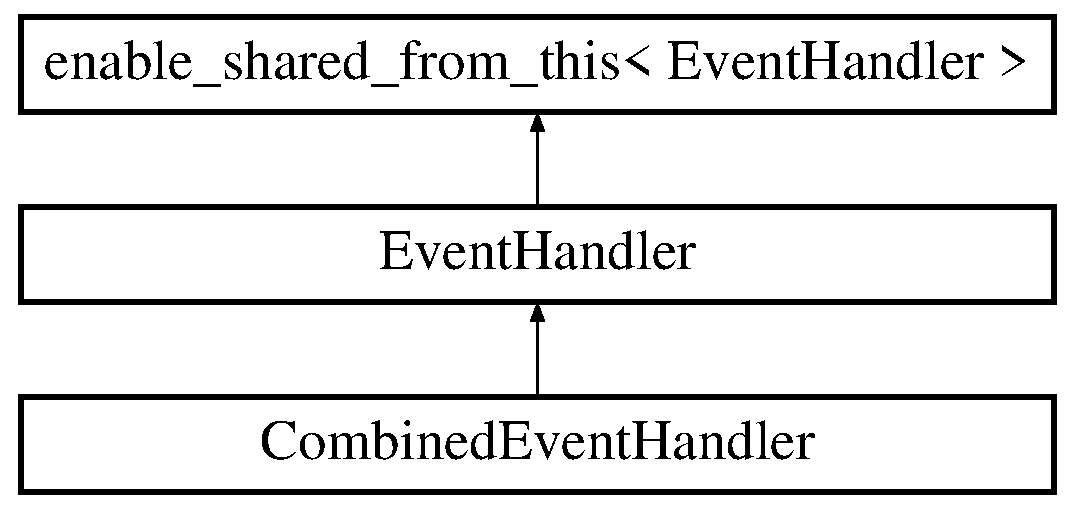
\includegraphics[height=3.000000cm]{classCombinedEventHandler}
\end{center}
\end{figure}
\subsection*{Public Member Functions}
\begin{DoxyCompactItemize}
\item 
\hypertarget{classCombinedEventHandler_ad45f2a5d0eb584f62d94de4c3d589a80}{{\bfseries Combined\+Event\+Handler} (shared\+\_\+ptr$<$ \hyperlink{structEventHandler}{Event\+Handler} $>$ first, shared\+\_\+ptr$<$ \hyperlink{structEventHandler}{Event\+Handler} $>$ second)}\label{classCombinedEventHandler_ad45f2a5d0eb584f62d94de4c3d589a80}

\item 
virtual bool \hyperlink{classCombinedEventHandler_a89f264f41a9de7162618e7549b24c82d}{handle\+Mouse\+Up} (\hyperlink{structMouseUpEvent}{Mouse\+Up\+Event} \&\hyperlink{unionSDL__Event}{event}) override
\begin{DoxyCompactList}\small\item\em Write what the function does here. \end{DoxyCompactList}\item 
virtual bool \hyperlink{classCombinedEventHandler_a7b4e923b77ac7c961d9919e4f169bf1a}{handle\+Mouse\+Down} (\hyperlink{structMouseDownEvent}{Mouse\+Down\+Event} \&\hyperlink{unionSDL__Event}{event}) override
\begin{DoxyCompactList}\small\item\em Write what the function does here. \end{DoxyCompactList}\item 
virtual bool \hyperlink{classCombinedEventHandler_ae7678e61d3ac2b416307bc5d4797fcdf}{handle\+Mouse\+Move} (\hyperlink{structMouseMoveEvent}{Mouse\+Move\+Event} \&\hyperlink{unionSDL__Event}{event}) override
\begin{DoxyCompactList}\small\item\em Write what the function does here. \end{DoxyCompactList}\item 
virtual bool \hyperlink{classCombinedEventHandler_a3f1d2344f2348a83242576eb9f9f81f6}{handle\+Mouse\+Scroll} (\hyperlink{structMouseScrollEvent}{Mouse\+Scroll\+Event} \&\hyperlink{unionSDL__Event}{event}) override
\begin{DoxyCompactList}\small\item\em Write what the function does here. \end{DoxyCompactList}\item 
virtual bool \hyperlink{classCombinedEventHandler_aa4fc97e377238948995cf04b10816094}{handle\+Key\+Up} (\hyperlink{classKeyUpEvent}{Key\+Up\+Event} \&\hyperlink{unionSDL__Event}{event}) override
\begin{DoxyCompactList}\small\item\em Write what the function does here. \end{DoxyCompactList}\item 
virtual bool \hyperlink{classCombinedEventHandler_a12c529bbe80bc54ffb0479b11c4cb896}{handle\+Key\+Down} (\hyperlink{classKeyDownEvent}{Key\+Down\+Event} \&\hyperlink{unionSDL__Event}{event}) override
\begin{DoxyCompactList}\small\item\em Write what the function does here. \end{DoxyCompactList}\item 
virtual bool \hyperlink{classCombinedEventHandler_a33f19194d740dc1a9af2f05fe00243bb}{handle\+Key\+Press} (\hyperlink{structKeyPressEvent}{Key\+Press\+Event} \&\hyperlink{unionSDL__Event}{event}) override
\begin{DoxyCompactList}\small\item\em Write what the function does here. \end{DoxyCompactList}\item 
virtual bool \hyperlink{classCombinedEventHandler_aeb9ba179ea0ea968303387f085ff424c}{handle\+Quit} (\hyperlink{structQuitEvent}{Quit\+Event} \&\hyperlink{unionSDL__Event}{event}) override
\begin{DoxyCompactList}\small\item\em Write what the function does here. \end{DoxyCompactList}\end{DoxyCompactItemize}
\subsection*{Private Attributes}
\begin{DoxyCompactItemize}
\item 
\hypertarget{classCombinedEventHandler_a9a137fe3fb3af1e98bde49d167f96f40}{shared\+\_\+ptr$<$ \hyperlink{structEventHandler}{Event\+Handler} $>$ {\bfseries first}}\label{classCombinedEventHandler_a9a137fe3fb3af1e98bde49d167f96f40}

\item 
\hypertarget{classCombinedEventHandler_a9099834af829d75a109e680c5704c66a}{shared\+\_\+ptr$<$ \hyperlink{structEventHandler}{Event\+Handler} $>$ {\bfseries second}}\label{classCombinedEventHandler_a9099834af829d75a109e680c5704c66a}

\end{DoxyCompactItemize}


\subsection{Detailed Description}
Write what the function does here. 


\begin{DoxyRetVals}{Return values}
{\em (variable)} & (description of variable) \\
\hline
\end{DoxyRetVals}


Definition at line 368 of file event.\+h.



\subsection{Member Function Documentation}
\hypertarget{classCombinedEventHandler_a12c529bbe80bc54ffb0479b11c4cb896}{\index{Combined\+Event\+Handler@{Combined\+Event\+Handler}!handle\+Key\+Down@{handle\+Key\+Down}}
\index{handle\+Key\+Down@{handle\+Key\+Down}!Combined\+Event\+Handler@{Combined\+Event\+Handler}}
\subsubsection[{handle\+Key\+Down}]{\setlength{\rightskip}{0pt plus 5cm}virtual bool Combined\+Event\+Handler\+::handle\+Key\+Down (
\begin{DoxyParamCaption}
\item[{{\bf Key\+Down\+Event} \&}]{event}
\end{DoxyParamCaption}
)\hspace{0.3cm}{\ttfamily [inline]}, {\ttfamily [override]}, {\ttfamily [virtual]}}}\label{classCombinedEventHandler_a12c529bbe80bc54ffb0479b11c4cb896}


Write what the function does here. 


\begin{DoxyParams}{Parameters}
{\em event} & \\
\hline
\end{DoxyParams}

\begin{DoxyRetVals}{Return values}
{\em (variable)} & (description of variable) \\
\hline
\end{DoxyRetVals}


Implements \hyperlink{structEventHandler}{Event\+Handler}.



Definition at line 470 of file event.\+h.


\begin{DoxyCode}
471         \{
472 
473             \textcolor{keywordflow}{if}(first->handleKeyDown(event))
474             \{
475                 \textcolor{keywordflow}{return} \textcolor{keyword}{true};
476             \}
477             \textcolor{keywordflow}{return} second->handleKeyDown(event);
478         \}
\end{DoxyCode}
\hypertarget{classCombinedEventHandler_a33f19194d740dc1a9af2f05fe00243bb}{\index{Combined\+Event\+Handler@{Combined\+Event\+Handler}!handle\+Key\+Press@{handle\+Key\+Press}}
\index{handle\+Key\+Press@{handle\+Key\+Press}!Combined\+Event\+Handler@{Combined\+Event\+Handler}}
\subsubsection[{handle\+Key\+Press}]{\setlength{\rightskip}{0pt plus 5cm}virtual bool Combined\+Event\+Handler\+::handle\+Key\+Press (
\begin{DoxyParamCaption}
\item[{{\bf Key\+Press\+Event} \&}]{event}
\end{DoxyParamCaption}
)\hspace{0.3cm}{\ttfamily [inline]}, {\ttfamily [override]}, {\ttfamily [virtual]}}}\label{classCombinedEventHandler_a33f19194d740dc1a9af2f05fe00243bb}


Write what the function does here. 


\begin{DoxyParams}{Parameters}
{\em event} & \\
\hline
\end{DoxyParams}

\begin{DoxyRetVals}{Return values}
{\em (variable)} & (description of variable) \\
\hline
\end{DoxyRetVals}


Implements \hyperlink{structEventHandler}{Event\+Handler}.



Definition at line 487 of file event.\+h.


\begin{DoxyCode}
488         \{
489 
490             \textcolor{keywordflow}{if}(first->handleKeyPress(event))
491             \{
492                 \textcolor{keywordflow}{return} \textcolor{keyword}{true};
493             \}
494             \textcolor{keywordflow}{return} second->handleKeyPress(event);
495         \}
\end{DoxyCode}
\hypertarget{classCombinedEventHandler_aa4fc97e377238948995cf04b10816094}{\index{Combined\+Event\+Handler@{Combined\+Event\+Handler}!handle\+Key\+Up@{handle\+Key\+Up}}
\index{handle\+Key\+Up@{handle\+Key\+Up}!Combined\+Event\+Handler@{Combined\+Event\+Handler}}
\subsubsection[{handle\+Key\+Up}]{\setlength{\rightskip}{0pt plus 5cm}virtual bool Combined\+Event\+Handler\+::handle\+Key\+Up (
\begin{DoxyParamCaption}
\item[{{\bf Key\+Up\+Event} \&}]{event}
\end{DoxyParamCaption}
)\hspace{0.3cm}{\ttfamily [inline]}, {\ttfamily [override]}, {\ttfamily [virtual]}}}\label{classCombinedEventHandler_aa4fc97e377238948995cf04b10816094}


Write what the function does here. 


\begin{DoxyParams}{Parameters}
{\em event} & \\
\hline
\end{DoxyParams}

\begin{DoxyRetVals}{Return values}
{\em (variable)} & (description of variable) \\
\hline
\end{DoxyRetVals}


Implements \hyperlink{structEventHandler}{Event\+Handler}.



Definition at line 453 of file event.\+h.


\begin{DoxyCode}
454         \{
455 
456             \textcolor{keywordflow}{if}(first->handleKeyUp(event))
457             \{
458                 \textcolor{keywordflow}{return} \textcolor{keyword}{true};
459             \}
460             \textcolor{keywordflow}{return} second->handleKeyUp(event);
461         \}
\end{DoxyCode}
\hypertarget{classCombinedEventHandler_a7b4e923b77ac7c961d9919e4f169bf1a}{\index{Combined\+Event\+Handler@{Combined\+Event\+Handler}!handle\+Mouse\+Down@{handle\+Mouse\+Down}}
\index{handle\+Mouse\+Down@{handle\+Mouse\+Down}!Combined\+Event\+Handler@{Combined\+Event\+Handler}}
\subsubsection[{handle\+Mouse\+Down}]{\setlength{\rightskip}{0pt plus 5cm}virtual bool Combined\+Event\+Handler\+::handle\+Mouse\+Down (
\begin{DoxyParamCaption}
\item[{{\bf Mouse\+Down\+Event} \&}]{event}
\end{DoxyParamCaption}
)\hspace{0.3cm}{\ttfamily [inline]}, {\ttfamily [override]}, {\ttfamily [virtual]}}}\label{classCombinedEventHandler_a7b4e923b77ac7c961d9919e4f169bf1a}


Write what the function does here. 


\begin{DoxyParams}{Parameters}
{\em event} & \\
\hline
\end{DoxyParams}

\begin{DoxyRetVals}{Return values}
{\em (variable)} & (description of variable) \\
\hline
\end{DoxyRetVals}


Implements \hyperlink{structEventHandler}{Event\+Handler}.



Definition at line 402 of file event.\+h.


\begin{DoxyCode}
403         \{
404 
405             \textcolor{keywordflow}{if}(first->handleMouseDown(event))
406             \{
407                 \textcolor{keywordflow}{return} \textcolor{keyword}{true};
408             \}
409             \textcolor{keywordflow}{return} second->handleMouseDown(event);
410         \}
\end{DoxyCode}
\hypertarget{classCombinedEventHandler_ae7678e61d3ac2b416307bc5d4797fcdf}{\index{Combined\+Event\+Handler@{Combined\+Event\+Handler}!handle\+Mouse\+Move@{handle\+Mouse\+Move}}
\index{handle\+Mouse\+Move@{handle\+Mouse\+Move}!Combined\+Event\+Handler@{Combined\+Event\+Handler}}
\subsubsection[{handle\+Mouse\+Move}]{\setlength{\rightskip}{0pt plus 5cm}virtual bool Combined\+Event\+Handler\+::handle\+Mouse\+Move (
\begin{DoxyParamCaption}
\item[{{\bf Mouse\+Move\+Event} \&}]{event}
\end{DoxyParamCaption}
)\hspace{0.3cm}{\ttfamily [inline]}, {\ttfamily [override]}, {\ttfamily [virtual]}}}\label{classCombinedEventHandler_ae7678e61d3ac2b416307bc5d4797fcdf}


Write what the function does here. 


\begin{DoxyParams}{Parameters}
{\em event} & \\
\hline
\end{DoxyParams}

\begin{DoxyRetVals}{Return values}
{\em (variable)} & (description of variable) \\
\hline
\end{DoxyRetVals}


Implements \hyperlink{structEventHandler}{Event\+Handler}.



Definition at line 419 of file event.\+h.


\begin{DoxyCode}
420         \{
421 
422             \textcolor{keywordflow}{if}(first->handleMouseMove(event))
423             \{
424                 \textcolor{keywordflow}{return} \textcolor{keyword}{true};
425             \}
426             \textcolor{keywordflow}{return} second->handleMouseMove(event);
427         \}
\end{DoxyCode}
\hypertarget{classCombinedEventHandler_a3f1d2344f2348a83242576eb9f9f81f6}{\index{Combined\+Event\+Handler@{Combined\+Event\+Handler}!handle\+Mouse\+Scroll@{handle\+Mouse\+Scroll}}
\index{handle\+Mouse\+Scroll@{handle\+Mouse\+Scroll}!Combined\+Event\+Handler@{Combined\+Event\+Handler}}
\subsubsection[{handle\+Mouse\+Scroll}]{\setlength{\rightskip}{0pt plus 5cm}virtual bool Combined\+Event\+Handler\+::handle\+Mouse\+Scroll (
\begin{DoxyParamCaption}
\item[{{\bf Mouse\+Scroll\+Event} \&}]{event}
\end{DoxyParamCaption}
)\hspace{0.3cm}{\ttfamily [inline]}, {\ttfamily [override]}, {\ttfamily [virtual]}}}\label{classCombinedEventHandler_a3f1d2344f2348a83242576eb9f9f81f6}


Write what the function does here. 


\begin{DoxyParams}{Parameters}
{\em event} & \\
\hline
\end{DoxyParams}

\begin{DoxyRetVals}{Return values}
{\em (variable)} & (description of variable) \\
\hline
\end{DoxyRetVals}


Implements \hyperlink{structEventHandler}{Event\+Handler}.



Definition at line 436 of file event.\+h.


\begin{DoxyCode}
437         \{
438 
439             \textcolor{keywordflow}{if}(first->handleMouseScroll(event))
440             \{
441                 \textcolor{keywordflow}{return} \textcolor{keyword}{true};
442             \}
443             \textcolor{keywordflow}{return} second->handleMouseScroll(event);
444         \}
\end{DoxyCode}
\hypertarget{classCombinedEventHandler_a89f264f41a9de7162618e7549b24c82d}{\index{Combined\+Event\+Handler@{Combined\+Event\+Handler}!handle\+Mouse\+Up@{handle\+Mouse\+Up}}
\index{handle\+Mouse\+Up@{handle\+Mouse\+Up}!Combined\+Event\+Handler@{Combined\+Event\+Handler}}
\subsubsection[{handle\+Mouse\+Up}]{\setlength{\rightskip}{0pt plus 5cm}virtual bool Combined\+Event\+Handler\+::handle\+Mouse\+Up (
\begin{DoxyParamCaption}
\item[{{\bf Mouse\+Up\+Event} \&}]{event}
\end{DoxyParamCaption}
)\hspace{0.3cm}{\ttfamily [inline]}, {\ttfamily [override]}, {\ttfamily [virtual]}}}\label{classCombinedEventHandler_a89f264f41a9de7162618e7549b24c82d}


Write what the function does here. 


\begin{DoxyParams}{Parameters}
{\em event} & \\
\hline
\end{DoxyParams}

\begin{DoxyRetVals}{Return values}
{\em (variable)} & (description of variable) \\
\hline
\end{DoxyRetVals}


Implements \hyperlink{structEventHandler}{Event\+Handler}.



Definition at line 385 of file event.\+h.


\begin{DoxyCode}
386         \{
387 
388             \textcolor{keywordflow}{if}(first->handleMouseUp(event))
389             \{
390                 \textcolor{keywordflow}{return} \textcolor{keyword}{true};
391             \}
392             \textcolor{keywordflow}{return} second->handleMouseUp(event);
393         \}
\end{DoxyCode}
\hypertarget{classCombinedEventHandler_aeb9ba179ea0ea968303387f085ff424c}{\index{Combined\+Event\+Handler@{Combined\+Event\+Handler}!handle\+Quit@{handle\+Quit}}
\index{handle\+Quit@{handle\+Quit}!Combined\+Event\+Handler@{Combined\+Event\+Handler}}
\subsubsection[{handle\+Quit}]{\setlength{\rightskip}{0pt plus 5cm}virtual bool Combined\+Event\+Handler\+::handle\+Quit (
\begin{DoxyParamCaption}
\item[{{\bf Quit\+Event} \&}]{event}
\end{DoxyParamCaption}
)\hspace{0.3cm}{\ttfamily [inline]}, {\ttfamily [override]}, {\ttfamily [virtual]}}}\label{classCombinedEventHandler_aeb9ba179ea0ea968303387f085ff424c}


Write what the function does here. 


\begin{DoxyParams}{Parameters}
{\em event} & \\
\hline
\end{DoxyParams}

\begin{DoxyRetVals}{Return values}
{\em (variable)} & (description of variable) \\
\hline
\end{DoxyRetVals}


Implements \hyperlink{structEventHandler}{Event\+Handler}.



Definition at line 504 of file event.\+h.


\begin{DoxyCode}
505         \{
506 
507             \textcolor{keywordflow}{if}(first->handleQuit(event))
508             \{
509                 \textcolor{keywordflow}{return} \textcolor{keyword}{true};
510             \}
511             \textcolor{keywordflow}{return} second->handleQuit(event);
512         \}
\end{DoxyCode}


The documentation for this class was generated from the following file\+:\begin{DoxyCompactItemize}
\item 
event.\+h\end{DoxyCompactItemize}

\hypertarget{classCompressWriter}{\section{Compress\+Writer Class Reference}
\label{classCompressWriter}\index{Compress\+Writer@{Compress\+Writer}}
}
Inheritance diagram for Compress\+Writer\+:\begin{figure}[H]
\begin{center}
\leavevmode
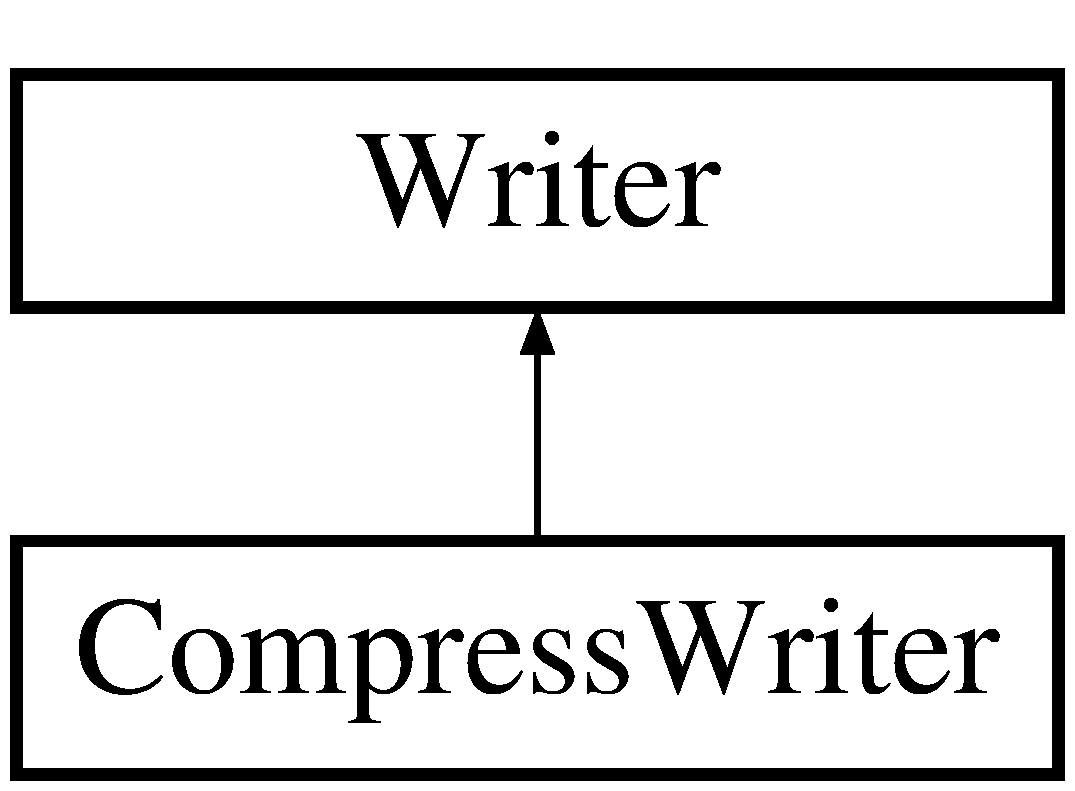
\includegraphics[height=2.000000cm]{classCompressWriter}
\end{center}
\end{figure}
\subsection*{Classes}
\begin{DoxyCompactItemize}
\item 
struct \hyperlink{structCompressWriter_1_1Match}{Match}
\end{DoxyCompactItemize}
\subsection*{Public Member Functions}
\begin{DoxyCompactItemize}
\item 
\hypertarget{classCompressWriter_a02f579d91e6ab012bbdba90481d327ef}{{\bfseries Compress\+Writer} (shared\+\_\+ptr$<$ \hyperlink{classWriter}{Writer} $>$ writer)}\label{classCompressWriter_a02f579d91e6ab012bbdba90481d327ef}

\item 
\hypertarget{classCompressWriter_a3e8580dad4dc5585d5f7af073d23e64b}{{\bfseries Compress\+Writer} (\hyperlink{classWriter}{Writer} \&writer)}\label{classCompressWriter_a3e8580dad4dc5585d5f7af073d23e64b}

\item 
\hypertarget{classCompressWriter_a23ba48ca17b9781ff531f7baeb08773e}{virtual void {\bfseries flush} () override}\label{classCompressWriter_a23ba48ca17b9781ff531f7baeb08773e}

\item 
\hypertarget{classCompressWriter_a3151658fd8e01af378e1d2ab12a24019}{virtual void {\bfseries write\+Byte} (uint8\+\_\+t v) override}\label{classCompressWriter_a3151658fd8e01af378e1d2ab12a24019}

\end{DoxyCompactItemize}
\subsection*{Private Member Functions}
\begin{DoxyCompactItemize}
\item 
\hypertarget{classCompressWriter_ab0fa055ce027b0f5be42531a285e2217}{size\+\_\+t {\bfseries get\+Actual\+Location} (size\+\_\+t l)}\label{classCompressWriter_ab0fa055ce027b0f5be42531a285e2217}

\item 
\hypertarget{classCompressWriter_a7c45f54c89b0e3ddac53f4ee95effa41}{void {\bfseries add\+Byte} (uint\+\_\+fast8\+\_\+t v)}\label{classCompressWriter_a7c45f54c89b0e3ddac53f4ee95effa41}

\item 
\hypertarget{classCompressWriter_a4e97ecc6a294aa87d685ce422cef6c56}{\hyperlink{structCompressWriter_1_1Match}{Match} {\bfseries get\+Biggest\+Match} ()}\label{classCompressWriter_a4e97ecc6a294aa87d685ce422cef6c56}

\item 
\hypertarget{classCompressWriter_ab958684312e2c0b9be302a1331410210}{void {\bfseries write\+Code} ()}\label{classCompressWriter_ab958684312e2c0b9be302a1331410210}

\end{DoxyCompactItemize}
\subsection*{Private Attributes}
\begin{DoxyCompactItemize}
\item 
\hypertarget{classCompressWriter_ad0c42284addda151ec815efa9eb1b333}{size\+\_\+t {\bfseries location}}\label{classCompressWriter_ad0c42284addda151ec815efa9eb1b333}

\item 
\hypertarget{classCompressWriter_afa45b760576d6845b4f955ea486d603c}{shared\+\_\+ptr$<$ \hyperlink{classWriter}{Writer} $>$ {\bfseries writer}}\label{classCompressWriter_afa45b760576d6845b4f955ea486d603c}

\item 
\hypertarget{classCompressWriter_a4a42d0a68afca7b21ac9edea6a6d465e}{\hyperlink{classcircularDeque}{circular\+Deque}$<$ uint\+\_\+fast8\+\_\+t, \\*
buffer\+Size+1 $>$ {\bfseries current\+Input}}\label{classCompressWriter_a4a42d0a68afca7b21ac9edea6a6d465e}

\item 
\hypertarget{classCompressWriter_a6dea17049f70649520ca9fd02931a5e1}{\hyperlink{classcircularDeque}{circular\+Deque}$<$ uint\+\_\+fast8\+\_\+t, \\*
buffer\+Size+2 $>$ {\bfseries buffer}}\label{classCompressWriter_a6dea17049f70649520ca9fd02931a5e1}

\item 
\hypertarget{classCompressWriter_a130499c9d22e1461044dd4316edfb50c}{list$<$ size\+\_\+t $>$ {\bfseries nodes} \mbox{[}uint8\+\_\+max+1\mbox{]}}\label{classCompressWriter_a130499c9d22e1461044dd4316edfb50c}

\end{DoxyCompactItemize}
\subsection*{Static Private Attributes}
\begin{DoxyCompactItemize}
\item 
\hypertarget{classCompressWriter_ace86be05e5886cfd42f77a5091c06b7a}{static constexpr int {\bfseries uint8\+\_\+max} = (1 $<$$<$ 8) -\/ 1}\label{classCompressWriter_ace86be05e5886cfd42f77a5091c06b7a}

\item 
\hypertarget{classCompressWriter_a96d2b6c2db5e69b996be1fefa7f337cb}{static constexpr size\+\_\+t {\bfseries buffer\+Size} = L\+Z77\+Code\+Type\+::max\+Offset + 1}\label{classCompressWriter_a96d2b6c2db5e69b996be1fefa7f337cb}

\end{DoxyCompactItemize}


\subsection{Detailed Description}


Definition at line 170 of file compressed\+\_\+stream.\+h.



The documentation for this class was generated from the following file\+:\begin{DoxyCompactItemize}
\item 
compressed\+\_\+stream.\+h\end{DoxyCompactItemize}

\hypertarget{structConnection}{\section{Connection Struct Reference}
\label{structConnection}\index{Connection@{Connection}}
}
\subsection*{Public Member Functions}
\begin{DoxyCompactItemize}
\item 
\hypertarget{structConnection_a5d69f2efa52f09b449af20c9479d67f8}{bool {\bfseries exists} () const }\label{structConnection_a5d69f2efa52f09b449af20c9479d67f8}

\item 
\hypertarget{structConnection_aaeb38386d09fdcd4d9eb70f58a31a8ed}{{\bfseries Connection} (Line $\ast$l, \hyperlink{structNode}{Node} $\ast$d)}\label{structConnection_aaeb38386d09fdcd4d9eb70f58a31a8ed}

\item 
\hypertarget{structConnection_aa865a13af12c712d04723871157205ae}{{\bfseries Connection} (const \hyperlink{structConnection}{Connection} \&c)}\label{structConnection_aa865a13af12c712d04723871157205ae}

\end{DoxyCompactItemize}
\subsection*{Public Attributes}
\begin{DoxyCompactItemize}
\item 
\hypertarget{structConnection_ac58f77f98bae33bc33702f909aa08535}{Line $\ast$ {\bfseries line}}\label{structConnection_ac58f77f98bae33bc33702f909aa08535}

\item 
\hypertarget{structConnection_a76ec6b5abe73168d8cad263d745524b3}{\hyperlink{structNode}{Node} $\ast$ {\bfseries dest}}\label{structConnection_a76ec6b5abe73168d8cad263d745524b3}

\end{DoxyCompactItemize}
\subsection*{Friends}
\begin{DoxyCompactItemize}
\item 
\hypertarget{structConnection_a43649da031123d524f6605d2b0b4ebc8}{ostream \& {\bfseries operator$<$$<$} (ostream \&, const \hyperlink{structConnection}{Connection} \&)}\label{structConnection_a43649da031123d524f6605d2b0b4ebc8}

\end{DoxyCompactItemize}


\subsection{Detailed Description}


Definition at line 31 of file structs.\+h.



The documentation for this struct was generated from the following file\+:\begin{DoxyCompactItemize}
\item 
headers/structs.\+h\end{DoxyCompactItemize}

\hypertarget{classcircularDeque_1_1const__iterator}{\section{circular\+Deque$<$ T, array\+Size $>$\+:\+:const\+\_\+iterator Class Reference}
\label{classcircularDeque_1_1const__iterator}\index{circular\+Deque$<$ T, array\+Size $>$\+::const\+\_\+iterator@{circular\+Deque$<$ T, array\+Size $>$\+::const\+\_\+iterator}}
}


Write what the function does here.  




{\ttfamily \#include $<$util.\+h$>$}

Inheritance diagram for circular\+Deque$<$ T, array\+Size $>$\+:\+:const\+\_\+iterator\+:\begin{figure}[H]
\begin{center}
\leavevmode
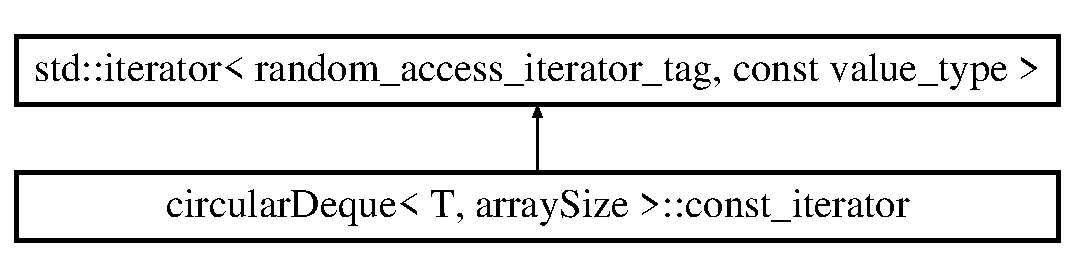
\includegraphics[height=2.000000cm]{classcircularDeque_1_1const__iterator}
\end{center}
\end{figure}
\subsection*{Public Member Functions}
\begin{DoxyCompactItemize}
\item 
\hypertarget{classcircularDeque_1_1const__iterator_a53e008033bdfbae4dd83c5e9de26652b}{{\bfseries const\+\_\+iterator} (const \hyperlink{classcircularDeque_1_1iterator}{iterator} \&v)}\label{classcircularDeque_1_1const__iterator_a53e008033bdfbae4dd83c5e9de26652b}

\item 
\hyperlink{classcircularDeque_1_1const__iterator}{const\+\_\+iterator} \& \hyperlink{classcircularDeque_1_1const__iterator_aaa9b3f1937d17f6f12f9986c477f89f5}{operator+=} (difference\+\_\+type n)
\begin{DoxyCompactList}\small\item\em Write what the function does here. \end{DoxyCompactList}\item 
\hyperlink{classcircularDeque_1_1const__iterator}{const\+\_\+iterator} \& \hyperlink{classcircularDeque_1_1const__iterator_a4e4380fcc95e65534c39c83b93f708f8}{operator-\/=} (difference\+\_\+type n)
\begin{DoxyCompactList}\small\item\em Write what the function does here. \end{DoxyCompactList}\item 
\hypertarget{classcircularDeque_1_1const__iterator_a3b2d9d2083342f3b378e87ea8fb271f3}{difference\+\_\+type {\bfseries operator-\/} (const \hyperlink{classcircularDeque_1_1const__iterator}{const\+\_\+iterator} \&r) const }\label{classcircularDeque_1_1const__iterator_a3b2d9d2083342f3b378e87ea8fb271f3}

\item 
const T \& \hyperlink{classcircularDeque_1_1const__iterator_a0c30a5251f3b952fc2438e3f01c4294f}{operator\mbox{[}$\,$\mbox{]}} (difference\+\_\+type n) const 
\begin{DoxyCompactList}\small\item\em Write what the function does here. \end{DoxyCompactList}\item 
const T \& \hyperlink{classcircularDeque_1_1const__iterator_af221298ee852c28ba884b18bd564c381}{operator$\ast$} () const 
\begin{DoxyCompactList}\small\item\em Write what the function does here. \end{DoxyCompactList}\item 
const T $\ast$ \hyperlink{classcircularDeque_1_1const__iterator_a99a687821e6b8356695374eb60a17644}{operator-\/$>$} () const 
\begin{DoxyCompactList}\small\item\em Write what the function does here. \end{DoxyCompactList}\item 
const \hyperlink{classcircularDeque_1_1const__iterator}{const\+\_\+iterator} \& \hyperlink{classcircularDeque_1_1const__iterator_af3164e3b086675a27892f4de0f5cb07a}{operator-\/-\/} ()
\begin{DoxyCompactList}\small\item\em Write what the function does here. \end{DoxyCompactList}\item 
\hyperlink{classcircularDeque_1_1const__iterator}{const\+\_\+iterator} \hyperlink{classcircularDeque_1_1const__iterator_ae8a986da58f120a06319332eca03c106}{operator-\/-\/} (int)
\begin{DoxyCompactList}\small\item\em Write what the function does here. \end{DoxyCompactList}\item 
const \hyperlink{classcircularDeque_1_1const__iterator}{const\+\_\+iterator} \& \hyperlink{classcircularDeque_1_1const__iterator_a1e1da24d7054467036d20a00c453c219}{operator++} ()
\begin{DoxyCompactList}\small\item\em Write what the function does here. \end{DoxyCompactList}\item 
\hyperlink{classcircularDeque_1_1const__iterator}{const\+\_\+iterator} \hyperlink{classcircularDeque_1_1const__iterator_a58909e8bf739c88361ba315c0b2e8e23}{operator++} (int)
\begin{DoxyCompactList}\small\item\em Write what the function does here. \end{DoxyCompactList}\end{DoxyCompactItemize}
\subsection*{Private Member Functions}
\begin{DoxyCompactItemize}
\item 
\hypertarget{classcircularDeque_1_1const__iterator_ac661ca71e0cc8321160e4364884fccda}{{\bfseries const\+\_\+iterator} (const \hyperlink{classcircularDeque}{circular\+Deque} $\ast$container, size\+\_\+t index)}\label{classcircularDeque_1_1const__iterator_ac661ca71e0cc8321160e4364884fccda}

\end{DoxyCompactItemize}
\subsection*{Private Attributes}
\begin{DoxyCompactItemize}
\item 
\hypertarget{classcircularDeque_1_1const__iterator_a60e5de271a30a0e308d405d719e24415}{const \hyperlink{classcircularDeque}{circular\+Deque} $\ast$ {\bfseries container}}\label{classcircularDeque_1_1const__iterator_a60e5de271a30a0e308d405d719e24415}

\item 
\hypertarget{classcircularDeque_1_1const__iterator_ad1106c610ff36cffdc47a9cd90db6260}{size\+\_\+t {\bfseries index}}\label{classcircularDeque_1_1const__iterator_ad1106c610ff36cffdc47a9cd90db6260}

\end{DoxyCompactItemize}
\subsection*{Friends}
\begin{DoxyCompactItemize}
\item 
\hypertarget{classcircularDeque_1_1const__iterator_aa63d8b47e75b076d05ec6aa14e29109b}{class {\bfseries circular\+Deque}}\label{classcircularDeque_1_1const__iterator_aa63d8b47e75b076d05ec6aa14e29109b}

\item 
\hyperlink{classcircularDeque_1_1const__iterator}{const\+\_\+iterator} \hyperlink{classcircularDeque_1_1const__iterator_a691016b314e13f42d0bb408060c49057}{operator+} (difference\+\_\+type n, \hyperlink{classcircularDeque_1_1const__iterator}{const\+\_\+iterator} i)
\begin{DoxyCompactList}\small\item\em Write what the function does here. \end{DoxyCompactList}\item 
\hyperlink{classcircularDeque_1_1const__iterator}{const\+\_\+iterator} \hyperlink{classcircularDeque_1_1const__iterator_a1ce501f5fc02fd634576dddb7afdc09a}{operator+} (\hyperlink{classcircularDeque_1_1const__iterator}{const\+\_\+iterator} i, difference\+\_\+type n)
\begin{DoxyCompactList}\small\item\em Write what the function does here. \end{DoxyCompactList}\item 
\hyperlink{classcircularDeque_1_1const__iterator}{const\+\_\+iterator} \hyperlink{classcircularDeque_1_1const__iterator_a39577c462b0d4115f031e1bdfb7b19b5}{operator-\/} (\hyperlink{classcircularDeque_1_1const__iterator}{const\+\_\+iterator} i, difference\+\_\+type n)
\begin{DoxyCompactList}\small\item\em Write what the function does here. \end{DoxyCompactList}\item 
bool \hyperlink{classcircularDeque_1_1const__iterator_ac7550bfcb9c7fd7ce95bb5d0d45bb076}{operator==} (const \hyperlink{classcircularDeque_1_1const__iterator}{const\+\_\+iterator} \&l, const \hyperlink{classcircularDeque_1_1const__iterator}{const\+\_\+iterator} \&r)
\begin{DoxyCompactList}\small\item\em Write what the function does here. \end{DoxyCompactList}\item 
bool \hyperlink{classcircularDeque_1_1const__iterator_af9237358f8dba2a676cc09f2ae028e0e}{operator!=} (const \hyperlink{classcircularDeque_1_1const__iterator}{const\+\_\+iterator} \&l, const \hyperlink{classcircularDeque_1_1const__iterator}{const\+\_\+iterator} \&r)
\begin{DoxyCompactList}\small\item\em Write what the function does here. \end{DoxyCompactList}\item 
bool \hyperlink{classcircularDeque_1_1const__iterator_ae3fcb1c6db8f72c42e0830aa4d8a5bd9}{operator$>$} (const \hyperlink{classcircularDeque_1_1const__iterator}{const\+\_\+iterator} \&l, const \hyperlink{classcircularDeque_1_1const__iterator}{const\+\_\+iterator} \&r)
\begin{DoxyCompactList}\small\item\em Write what the function does here. \end{DoxyCompactList}\item 
bool \hyperlink{classcircularDeque_1_1const__iterator_ab9e286a09c563b3cc6464fce11884a0e}{operator$>$=} (const \hyperlink{classcircularDeque_1_1const__iterator}{const\+\_\+iterator} \&l, const \hyperlink{classcircularDeque_1_1const__iterator}{const\+\_\+iterator} \&r)
\begin{DoxyCompactList}\small\item\em Write what the function does here. \end{DoxyCompactList}\item 
bool \hyperlink{classcircularDeque_1_1const__iterator_a0ff653fe6b36c48d70e1d4fd88fb80c7}{operator$<$} (const \hyperlink{classcircularDeque_1_1const__iterator}{const\+\_\+iterator} \&l, const \hyperlink{classcircularDeque_1_1const__iterator}{const\+\_\+iterator} \&r)
\begin{DoxyCompactList}\small\item\em Write what the function does here. \end{DoxyCompactList}\item 
bool \hyperlink{classcircularDeque_1_1const__iterator_a9bfb32fe108f74ef4d6d9ef242ef9751}{operator$<$=} (const \hyperlink{classcircularDeque_1_1const__iterator}{const\+\_\+iterator} \&l, const \hyperlink{classcircularDeque_1_1const__iterator}{const\+\_\+iterator} \&r)
\begin{DoxyCompactList}\small\item\em Write what the function does here. \end{DoxyCompactList}\end{DoxyCompactItemize}


\subsection{Detailed Description}
\subsubsection*{template$<$typename T, size\+\_\+t array\+Size$>$class circular\+Deque$<$ T, array\+Size $>$\+::const\+\_\+iterator}

Write what the function does here. 


\begin{DoxyParams}{Parameters}
{\em random\+\_\+access\+\_\+iterator\+\_\+tag} & \\
\hline
\end{DoxyParams}

\begin{DoxyRetVals}{Return values}
{\em (variable)} & (description of variable) \\
\hline
\end{DoxyRetVals}


Definition at line 589 of file util.\+h.



\subsection{Member Function Documentation}
\hypertarget{classcircularDeque_1_1const__iterator_af221298ee852c28ba884b18bd564c381}{\index{circular\+Deque\+::const\+\_\+iterator@{circular\+Deque\+::const\+\_\+iterator}!operator$\ast$@{operator$\ast$}}
\index{operator$\ast$@{operator$\ast$}!circular\+Deque\+::const\+\_\+iterator@{circular\+Deque\+::const\+\_\+iterator}}
\subsubsection[{operator$\ast$}]{\setlength{\rightskip}{0pt plus 5cm}template$<$typename T, size\+\_\+t array\+Size$>$ const T\& {\bf circular\+Deque}$<$ T, array\+Size $>$\+::const\+\_\+iterator\+::operator$\ast$ (
\begin{DoxyParamCaption}
{}
\end{DoxyParamCaption}
) const\hspace{0.3cm}{\ttfamily [inline]}}}\label{classcircularDeque_1_1const__iterator_af221298ee852c28ba884b18bd564c381}


Write what the function does here. 


\begin{DoxyRetVals}{Return values}
{\em (variable)} & (description of variable) \\
\hline
\end{DoxyRetVals}


Definition at line 729 of file util.\+h.


\begin{DoxyCode}
730         \{
731             \textcolor{keywordflow}{return} container->array[index];
732         \}
\end{DoxyCode}
\hypertarget{classcircularDeque_1_1const__iterator_a1e1da24d7054467036d20a00c453c219}{\index{circular\+Deque\+::const\+\_\+iterator@{circular\+Deque\+::const\+\_\+iterator}!operator++@{operator++}}
\index{operator++@{operator++}!circular\+Deque\+::const\+\_\+iterator@{circular\+Deque\+::const\+\_\+iterator}}
\subsubsection[{operator++}]{\setlength{\rightskip}{0pt plus 5cm}template$<$typename T, size\+\_\+t array\+Size$>$ const {\bf const\+\_\+iterator}\& {\bf circular\+Deque}$<$ T, array\+Size $>$\+::const\+\_\+iterator\+::operator++ (
\begin{DoxyParamCaption}
{}
\end{DoxyParamCaption}
)\hspace{0.3cm}{\ttfamily [inline]}}}\label{classcircularDeque_1_1const__iterator_a1e1da24d7054467036d20a00c453c219}


Write what the function does here. 


\begin{DoxyRetVals}{Return values}
{\em (variable)} & (description of variable) \\
\hline
\end{DoxyRetVals}


Definition at line 792 of file util.\+h.


\begin{DoxyCode}
793         \{
794 
795             \textcolor{keywordflow}{if}(index >= arraySize - 1)
796             \{
797                 index = 0;
798             \}
799 
800             \textcolor{keywordflow}{else}
801             \{
802                 index++;
803             \}
804             \textcolor{keywordflow}{return} *\textcolor{keyword}{this};
805         \}
\end{DoxyCode}
\hypertarget{classcircularDeque_1_1const__iterator_a58909e8bf739c88361ba315c0b2e8e23}{\index{circular\+Deque\+::const\+\_\+iterator@{circular\+Deque\+::const\+\_\+iterator}!operator++@{operator++}}
\index{operator++@{operator++}!circular\+Deque\+::const\+\_\+iterator@{circular\+Deque\+::const\+\_\+iterator}}
\subsubsection[{operator++}]{\setlength{\rightskip}{0pt plus 5cm}template$<$typename T, size\+\_\+t array\+Size$>$ {\bf const\+\_\+iterator} {\bf circular\+Deque}$<$ T, array\+Size $>$\+::const\+\_\+iterator\+::operator++ (
\begin{DoxyParamCaption}
\item[{int}]{}
\end{DoxyParamCaption}
)\hspace{0.3cm}{\ttfamily [inline]}}}\label{classcircularDeque_1_1const__iterator_a58909e8bf739c88361ba315c0b2e8e23}


Write what the function does here. 


\begin{DoxyParams}{Parameters}
{\em int} & \\
\hline
\end{DoxyParams}

\begin{DoxyRetVals}{Return values}
{\em (variable)} & (description of variable) \\
\hline
\end{DoxyRetVals}


Definition at line 814 of file util.\+h.


\begin{DoxyCode}
815         \{
816             const\_iterator retval = *\textcolor{keyword}{this};
817 
818             \textcolor{keywordflow}{if}(index >= arraySize - 1)
819             \{
820                 index = 0;
821             \}
822 
823             \textcolor{keywordflow}{else}
824             \{
825                 index++;
826             \}
827             \textcolor{keywordflow}{return} retval;
828         \}
\end{DoxyCode}
\hypertarget{classcircularDeque_1_1const__iterator_aaa9b3f1937d17f6f12f9986c477f89f5}{\index{circular\+Deque\+::const\+\_\+iterator@{circular\+Deque\+::const\+\_\+iterator}!operator+=@{operator+=}}
\index{operator+=@{operator+=}!circular\+Deque\+::const\+\_\+iterator@{circular\+Deque\+::const\+\_\+iterator}}
\subsubsection[{operator+=}]{\setlength{\rightskip}{0pt plus 5cm}template$<$typename T, size\+\_\+t array\+Size$>$ {\bf const\+\_\+iterator}\& {\bf circular\+Deque}$<$ T, array\+Size $>$\+::const\+\_\+iterator\+::operator+= (
\begin{DoxyParamCaption}
\item[{difference\+\_\+type}]{n}
\end{DoxyParamCaption}
)\hspace{0.3cm}{\ttfamily [inline]}}}\label{classcircularDeque_1_1const__iterator_aaa9b3f1937d17f6f12f9986c477f89f5}


Write what the function does here. 


\begin{DoxyParams}{Parameters}
{\em n} & \\
\hline
\end{DoxyParams}

\begin{DoxyRetVals}{Return values}
{\em (variable)} & (description of variable) \\
\hline
\end{DoxyRetVals}


Definition at line 616 of file util.\+h.


\begin{DoxyCode}
617         \{
618 
619             \textcolor{keywordflow}{if}(-n > (difference\_type)index)
620             \{
621                 n = n % arraySize + arraySize;
622             \}
623             index += n;
624             index %= arraySize;
625 
626             \textcolor{keywordflow}{if}(index < 0)
627             \{
628                 index += arraySize;
629             \}
630             \textcolor{keywordflow}{return} *\textcolor{keyword}{this};
631         \}
\end{DoxyCode}
\hypertarget{classcircularDeque_1_1const__iterator_af3164e3b086675a27892f4de0f5cb07a}{\index{circular\+Deque\+::const\+\_\+iterator@{circular\+Deque\+::const\+\_\+iterator}!operator-\/-\/@{operator-\/-\/}}
\index{operator-\/-\/@{operator-\/-\/}!circular\+Deque\+::const\+\_\+iterator@{circular\+Deque\+::const\+\_\+iterator}}
\subsubsection[{operator-\/-\/}]{\setlength{\rightskip}{0pt plus 5cm}template$<$typename T, size\+\_\+t array\+Size$>$ const {\bf const\+\_\+iterator}\& {\bf circular\+Deque}$<$ T, array\+Size $>$\+::const\+\_\+iterator\+::operator-\/-\/ (
\begin{DoxyParamCaption}
{}
\end{DoxyParamCaption}
)\hspace{0.3cm}{\ttfamily [inline]}}}\label{classcircularDeque_1_1const__iterator_af3164e3b086675a27892f4de0f5cb07a}


Write what the function does here. 


\begin{DoxyRetVals}{Return values}
{\em (variable)} & (description of variable) \\
\hline
\end{DoxyRetVals}


Definition at line 749 of file util.\+h.


\begin{DoxyCode}
750         \{
751 
752             \textcolor{keywordflow}{if}(index == 0)
753             \{
754                 index = arraySize - 1;
755             \}
756 
757             \textcolor{keywordflow}{else}
758             \{
759                 index--;
760             \}
761             \textcolor{keywordflow}{return} *\textcolor{keyword}{this};
762         \}
\end{DoxyCode}
\hypertarget{classcircularDeque_1_1const__iterator_ae8a986da58f120a06319332eca03c106}{\index{circular\+Deque\+::const\+\_\+iterator@{circular\+Deque\+::const\+\_\+iterator}!operator-\/-\/@{operator-\/-\/}}
\index{operator-\/-\/@{operator-\/-\/}!circular\+Deque\+::const\+\_\+iterator@{circular\+Deque\+::const\+\_\+iterator}}
\subsubsection[{operator-\/-\/}]{\setlength{\rightskip}{0pt plus 5cm}template$<$typename T, size\+\_\+t array\+Size$>$ {\bf const\+\_\+iterator} {\bf circular\+Deque}$<$ T, array\+Size $>$\+::const\+\_\+iterator\+::operator-\/-\/ (
\begin{DoxyParamCaption}
\item[{int}]{}
\end{DoxyParamCaption}
)\hspace{0.3cm}{\ttfamily [inline]}}}\label{classcircularDeque_1_1const__iterator_ae8a986da58f120a06319332eca03c106}


Write what the function does here. 


\begin{DoxyParams}{Parameters}
{\em int} & \\
\hline
\end{DoxyParams}

\begin{DoxyRetVals}{Return values}
{\em (variable)} & (description of variable) \\
\hline
\end{DoxyRetVals}


Definition at line 771 of file util.\+h.


\begin{DoxyCode}
772         \{
773             const\_iterator retval = *\textcolor{keyword}{this};
774 
775             \textcolor{keywordflow}{if}(index == 0)
776             \{
777                 index = arraySize - 1;
778             \}
779 
780             \textcolor{keywordflow}{else}
781             \{
782                 index--;
783             \}
784             \textcolor{keywordflow}{return} retval;
785         \}
\end{DoxyCode}
\hypertarget{classcircularDeque_1_1const__iterator_a4e4380fcc95e65534c39c83b93f708f8}{\index{circular\+Deque\+::const\+\_\+iterator@{circular\+Deque\+::const\+\_\+iterator}!operator-\/=@{operator-\/=}}
\index{operator-\/=@{operator-\/=}!circular\+Deque\+::const\+\_\+iterator@{circular\+Deque\+::const\+\_\+iterator}}
\subsubsection[{operator-\/=}]{\setlength{\rightskip}{0pt plus 5cm}template$<$typename T, size\+\_\+t array\+Size$>$ {\bf const\+\_\+iterator}\& {\bf circular\+Deque}$<$ T, array\+Size $>$\+::const\+\_\+iterator\+::operator-\/= (
\begin{DoxyParamCaption}
\item[{difference\+\_\+type}]{n}
\end{DoxyParamCaption}
)\hspace{0.3cm}{\ttfamily [inline]}}}\label{classcircularDeque_1_1const__iterator_a4e4380fcc95e65534c39c83b93f708f8}


Write what the function does here. 


\begin{DoxyParams}{Parameters}
{\em n} & \\
\hline
\end{DoxyParams}

\begin{DoxyRetVals}{Return values}
{\em (variable)} & (description of variable) \\
\hline
\end{DoxyRetVals}


Definition at line 640 of file util.\+h.


\begin{DoxyCode}
641         \{
642             \textcolor{keywordflow}{return} *\textcolor{keyword}{this} += -n;
643         \}
\end{DoxyCode}
\hypertarget{classcircularDeque_1_1const__iterator_a99a687821e6b8356695374eb60a17644}{\index{circular\+Deque\+::const\+\_\+iterator@{circular\+Deque\+::const\+\_\+iterator}!operator-\/$>$@{operator-\/$>$}}
\index{operator-\/$>$@{operator-\/$>$}!circular\+Deque\+::const\+\_\+iterator@{circular\+Deque\+::const\+\_\+iterator}}
\subsubsection[{operator-\/$>$}]{\setlength{\rightskip}{0pt plus 5cm}template$<$typename T, size\+\_\+t array\+Size$>$ const T$\ast$ {\bf circular\+Deque}$<$ T, array\+Size $>$\+::const\+\_\+iterator\+::operator-\/$>$ (
\begin{DoxyParamCaption}
{}
\end{DoxyParamCaption}
) const\hspace{0.3cm}{\ttfamily [inline]}}}\label{classcircularDeque_1_1const__iterator_a99a687821e6b8356695374eb60a17644}


Write what the function does here. 


\begin{DoxyRetVals}{Return values}
{\em (variable)} & (description of variable) \\
\hline
\end{DoxyRetVals}


Definition at line 739 of file util.\+h.


\begin{DoxyCode}
740         \{
741             \textcolor{keywordflow}{return} container->array + index;
742         \}
\end{DoxyCode}
\hypertarget{classcircularDeque_1_1const__iterator_a0c30a5251f3b952fc2438e3f01c4294f}{\index{circular\+Deque\+::const\+\_\+iterator@{circular\+Deque\+::const\+\_\+iterator}!operator\mbox{[}$\,$\mbox{]}@{operator[]}}
\index{operator\mbox{[}$\,$\mbox{]}@{operator[]}!circular\+Deque\+::const\+\_\+iterator@{circular\+Deque\+::const\+\_\+iterator}}
\subsubsection[{operator[]}]{\setlength{\rightskip}{0pt plus 5cm}template$<$typename T, size\+\_\+t array\+Size$>$ const T\& {\bf circular\+Deque}$<$ T, array\+Size $>$\+::const\+\_\+iterator\+::operator\mbox{[}$\,$\mbox{]} (
\begin{DoxyParamCaption}
\item[{difference\+\_\+type}]{n}
\end{DoxyParamCaption}
) const\hspace{0.3cm}{\ttfamily [inline]}}}\label{classcircularDeque_1_1const__iterator_a0c30a5251f3b952fc2438e3f01c4294f}


Write what the function does here. 


\begin{DoxyParams}{Parameters}
{\em n} & \\
\hline
\end{DoxyParams}

\begin{DoxyRetVals}{Return values}
{\em (variable)} & (description of variable) \\
\hline
\end{DoxyRetVals}


Definition at line 719 of file util.\+h.


\begin{DoxyCode}
720         \{
721             \textcolor{keywordflow}{return} *(*\textcolor{keyword}{this} + n);
722         \}
\end{DoxyCode}


\subsection{Friends And Related Function Documentation}
\hypertarget{classcircularDeque_1_1const__iterator_af9237358f8dba2a676cc09f2ae028e0e}{\index{circular\+Deque\+::const\+\_\+iterator@{circular\+Deque\+::const\+\_\+iterator}!operator"!=@{operator"!=}}
\index{operator"!=@{operator"!=}!circular\+Deque\+::const\+\_\+iterator@{circular\+Deque\+::const\+\_\+iterator}}
\subsubsection[{operator"!=}]{\setlength{\rightskip}{0pt plus 5cm}template$<$typename T, size\+\_\+t array\+Size$>$ bool operator!= (
\begin{DoxyParamCaption}
\item[{const {\bf const\+\_\+iterator} \&}]{l, }
\item[{const {\bf const\+\_\+iterator} \&}]{r}
\end{DoxyParamCaption}
)\hspace{0.3cm}{\ttfamily [friend]}}}\label{classcircularDeque_1_1const__iterator_af9237358f8dba2a676cc09f2ae028e0e}


Write what the function does here. 


\begin{DoxyParams}{Parameters}
{\em l} & \\
\hline
{\em r} & \\
\hline
\end{DoxyParams}

\begin{DoxyRetVals}{Return values}
{\em (variable)} & (description of variable) \\
\hline
\end{DoxyRetVals}


Definition at line 851 of file util.\+h.


\begin{DoxyCode}
852         \{
853             \textcolor{keywordflow}{return} l.index != r.index;
854         \}
\end{DoxyCode}
\hypertarget{classcircularDeque_1_1const__iterator_a691016b314e13f42d0bb408060c49057}{\index{circular\+Deque\+::const\+\_\+iterator@{circular\+Deque\+::const\+\_\+iterator}!operator+@{operator+}}
\index{operator+@{operator+}!circular\+Deque\+::const\+\_\+iterator@{circular\+Deque\+::const\+\_\+iterator}}
\subsubsection[{operator+}]{\setlength{\rightskip}{0pt plus 5cm}template$<$typename T, size\+\_\+t array\+Size$>$ {\bf const\+\_\+iterator} operator+ (
\begin{DoxyParamCaption}
\item[{difference\+\_\+type}]{n, }
\item[{{\bf const\+\_\+iterator}}]{i}
\end{DoxyParamCaption}
)\hspace{0.3cm}{\ttfamily [friend]}}}\label{classcircularDeque_1_1const__iterator_a691016b314e13f42d0bb408060c49057}


Write what the function does here. 


\begin{DoxyParams}{Parameters}
{\em n} & \\
\hline
{\em i} & \\
\hline
\end{DoxyParams}

\begin{DoxyRetVals}{Return values}
{\em (variable)} & (description of variable) \\
\hline
\end{DoxyRetVals}


Definition at line 653 of file util.\+h.


\begin{DoxyCode}
654         \{
655             \textcolor{keywordflow}{return} i += n;
656         \}
\end{DoxyCode}
\hypertarget{classcircularDeque_1_1const__iterator_a1ce501f5fc02fd634576dddb7afdc09a}{\index{circular\+Deque\+::const\+\_\+iterator@{circular\+Deque\+::const\+\_\+iterator}!operator+@{operator+}}
\index{operator+@{operator+}!circular\+Deque\+::const\+\_\+iterator@{circular\+Deque\+::const\+\_\+iterator}}
\subsubsection[{operator+}]{\setlength{\rightskip}{0pt plus 5cm}template$<$typename T, size\+\_\+t array\+Size$>$ {\bf const\+\_\+iterator} operator+ (
\begin{DoxyParamCaption}
\item[{{\bf const\+\_\+iterator}}]{i, }
\item[{difference\+\_\+type}]{n}
\end{DoxyParamCaption}
)\hspace{0.3cm}{\ttfamily [friend]}}}\label{classcircularDeque_1_1const__iterator_a1ce501f5fc02fd634576dddb7afdc09a}


Write what the function does here. 


\begin{DoxyParams}{Parameters}
{\em i} & \\
\hline
{\em n} & \\
\hline
\end{DoxyParams}

\begin{DoxyRetVals}{Return values}
{\em (variable)} & (description of variable) \\
\hline
\end{DoxyRetVals}


Definition at line 666 of file util.\+h.


\begin{DoxyCode}
667         \{
668             \textcolor{keywordflow}{return} i += n;
669         \}
\end{DoxyCode}
\hypertarget{classcircularDeque_1_1const__iterator_a39577c462b0d4115f031e1bdfb7b19b5}{\index{circular\+Deque\+::const\+\_\+iterator@{circular\+Deque\+::const\+\_\+iterator}!operator-\/@{operator-\/}}
\index{operator-\/@{operator-\/}!circular\+Deque\+::const\+\_\+iterator@{circular\+Deque\+::const\+\_\+iterator}}
\subsubsection[{operator-\/}]{\setlength{\rightskip}{0pt plus 5cm}template$<$typename T, size\+\_\+t array\+Size$>$ {\bf const\+\_\+iterator} operator-\/ (
\begin{DoxyParamCaption}
\item[{{\bf const\+\_\+iterator}}]{i, }
\item[{difference\+\_\+type}]{n}
\end{DoxyParamCaption}
)\hspace{0.3cm}{\ttfamily [friend]}}}\label{classcircularDeque_1_1const__iterator_a39577c462b0d4115f031e1bdfb7b19b5}


Write what the function does here. 


\begin{DoxyParams}{Parameters}
{\em i} & \\
\hline
{\em n} & \\
\hline
\end{DoxyParams}

\begin{DoxyRetVals}{Return values}
{\em (variable)} & (description of variable) \\
\hline
\end{DoxyRetVals}


Definition at line 679 of file util.\+h.


\begin{DoxyCode}
680         \{
681             \textcolor{keywordflow}{return} i -= n;
682         \}
\end{DoxyCode}
\hypertarget{classcircularDeque_1_1const__iterator_a0ff653fe6b36c48d70e1d4fd88fb80c7}{\index{circular\+Deque\+::const\+\_\+iterator@{circular\+Deque\+::const\+\_\+iterator}!operator$<$@{operator$<$}}
\index{operator$<$@{operator$<$}!circular\+Deque\+::const\+\_\+iterator@{circular\+Deque\+::const\+\_\+iterator}}
\subsubsection[{operator$<$}]{\setlength{\rightskip}{0pt plus 5cm}template$<$typename T, size\+\_\+t array\+Size$>$ bool operator$<$ (
\begin{DoxyParamCaption}
\item[{const {\bf const\+\_\+iterator} \&}]{l, }
\item[{const {\bf const\+\_\+iterator} \&}]{r}
\end{DoxyParamCaption}
)\hspace{0.3cm}{\ttfamily [friend]}}}\label{classcircularDeque_1_1const__iterator_a0ff653fe6b36c48d70e1d4fd88fb80c7}


Write what the function does here. 


\begin{DoxyParams}{Parameters}
{\em l} & \\
\hline
{\em r} & \\
\hline
\end{DoxyParams}

\begin{DoxyRetVals}{Return values}
{\em (variable)} & (description of variable) \\
\hline
\end{DoxyRetVals}


Definition at line 890 of file util.\+h.


\begin{DoxyCode}
891         \{
892             \textcolor{keywordflow}{return} (l - r) < 0;
893         \}
\end{DoxyCode}
\hypertarget{classcircularDeque_1_1const__iterator_a9bfb32fe108f74ef4d6d9ef242ef9751}{\index{circular\+Deque\+::const\+\_\+iterator@{circular\+Deque\+::const\+\_\+iterator}!operator$<$=@{operator$<$=}}
\index{operator$<$=@{operator$<$=}!circular\+Deque\+::const\+\_\+iterator@{circular\+Deque\+::const\+\_\+iterator}}
\subsubsection[{operator$<$=}]{\setlength{\rightskip}{0pt plus 5cm}template$<$typename T, size\+\_\+t array\+Size$>$ bool operator$<$= (
\begin{DoxyParamCaption}
\item[{const {\bf const\+\_\+iterator} \&}]{l, }
\item[{const {\bf const\+\_\+iterator} \&}]{r}
\end{DoxyParamCaption}
)\hspace{0.3cm}{\ttfamily [friend]}}}\label{classcircularDeque_1_1const__iterator_a9bfb32fe108f74ef4d6d9ef242ef9751}


Write what the function does here. 


\begin{DoxyParams}{Parameters}
{\em l} & \\
\hline
{\em r} & \\
\hline
\end{DoxyParams}

\begin{DoxyRetVals}{Return values}
{\em (variable)} & (description of variable) \\
\hline
\end{DoxyRetVals}


Definition at line 903 of file util.\+h.


\begin{DoxyCode}
904         \{
905             \textcolor{keywordflow}{return} (l - r) <= 0;
906         \}
\end{DoxyCode}
\hypertarget{classcircularDeque_1_1const__iterator_ac7550bfcb9c7fd7ce95bb5d0d45bb076}{\index{circular\+Deque\+::const\+\_\+iterator@{circular\+Deque\+::const\+\_\+iterator}!operator==@{operator==}}
\index{operator==@{operator==}!circular\+Deque\+::const\+\_\+iterator@{circular\+Deque\+::const\+\_\+iterator}}
\subsubsection[{operator==}]{\setlength{\rightskip}{0pt plus 5cm}template$<$typename T, size\+\_\+t array\+Size$>$ bool operator== (
\begin{DoxyParamCaption}
\item[{const {\bf const\+\_\+iterator} \&}]{l, }
\item[{const {\bf const\+\_\+iterator} \&}]{r}
\end{DoxyParamCaption}
)\hspace{0.3cm}{\ttfamily [friend]}}}\label{classcircularDeque_1_1const__iterator_ac7550bfcb9c7fd7ce95bb5d0d45bb076}


Write what the function does here. 


\begin{DoxyParams}{Parameters}
{\em l} & \\
\hline
{\em r} & \\
\hline
\end{DoxyParams}

\begin{DoxyRetVals}{Return values}
{\em (variable)} & (description of variable) \\
\hline
\end{DoxyRetVals}


Definition at line 838 of file util.\+h.


\begin{DoxyCode}
839         \{
840             \textcolor{keywordflow}{return} l.index == r.index;
841         \}
\end{DoxyCode}
\hypertarget{classcircularDeque_1_1const__iterator_ae3fcb1c6db8f72c42e0830aa4d8a5bd9}{\index{circular\+Deque\+::const\+\_\+iterator@{circular\+Deque\+::const\+\_\+iterator}!operator$>$@{operator$>$}}
\index{operator$>$@{operator$>$}!circular\+Deque\+::const\+\_\+iterator@{circular\+Deque\+::const\+\_\+iterator}}
\subsubsection[{operator$>$}]{\setlength{\rightskip}{0pt plus 5cm}template$<$typename T, size\+\_\+t array\+Size$>$ bool operator$>$ (
\begin{DoxyParamCaption}
\item[{const {\bf const\+\_\+iterator} \&}]{l, }
\item[{const {\bf const\+\_\+iterator} \&}]{r}
\end{DoxyParamCaption}
)\hspace{0.3cm}{\ttfamily [friend]}}}\label{classcircularDeque_1_1const__iterator_ae3fcb1c6db8f72c42e0830aa4d8a5bd9}


Write what the function does here. 


\begin{DoxyParams}{Parameters}
{\em l} & \\
\hline
{\em r} & \\
\hline
\end{DoxyParams}

\begin{DoxyRetVals}{Return values}
{\em (variable)} & (description of variable) \\
\hline
\end{DoxyRetVals}


Definition at line 864 of file util.\+h.


\begin{DoxyCode}
865         \{
866             \textcolor{keywordflow}{return} (l - r) > 0;
867         \}
\end{DoxyCode}
\hypertarget{classcircularDeque_1_1const__iterator_ab9e286a09c563b3cc6464fce11884a0e}{\index{circular\+Deque\+::const\+\_\+iterator@{circular\+Deque\+::const\+\_\+iterator}!operator$>$=@{operator$>$=}}
\index{operator$>$=@{operator$>$=}!circular\+Deque\+::const\+\_\+iterator@{circular\+Deque\+::const\+\_\+iterator}}
\subsubsection[{operator$>$=}]{\setlength{\rightskip}{0pt plus 5cm}template$<$typename T, size\+\_\+t array\+Size$>$ bool operator$>$= (
\begin{DoxyParamCaption}
\item[{const {\bf const\+\_\+iterator} \&}]{l, }
\item[{const {\bf const\+\_\+iterator} \&}]{r}
\end{DoxyParamCaption}
)\hspace{0.3cm}{\ttfamily [friend]}}}\label{classcircularDeque_1_1const__iterator_ab9e286a09c563b3cc6464fce11884a0e}


Write what the function does here. 


\begin{DoxyParams}{Parameters}
{\em l} & \\
\hline
{\em r} & \\
\hline
\end{DoxyParams}

\begin{DoxyRetVals}{Return values}
{\em (variable)} & (description of variable) \\
\hline
\end{DoxyRetVals}


Definition at line 877 of file util.\+h.


\begin{DoxyCode}
878         \{
879             \textcolor{keywordflow}{return} (l - r) >= 0;
880         \}
\end{DoxyCode}


The documentation for this class was generated from the following file\+:\begin{DoxyCompactItemize}
\item 
util.\+h\end{DoxyCompactItemize}

\hypertarget{classMesh__t_1_1const__iterator}{\section{Mesh\+\_\+t\+:\+:const\+\_\+iterator Class Reference}
\label{classMesh__t_1_1const__iterator}\index{Mesh\+\_\+t\+::const\+\_\+iterator@{Mesh\+\_\+t\+::const\+\_\+iterator}}
}


Write what the function does here.  




{\ttfamily \#include $<$mesh.\+h$>$}

Inheritance diagram for Mesh\+\_\+t\+:\+:const\+\_\+iterator\+:\begin{figure}[H]
\begin{center}
\leavevmode
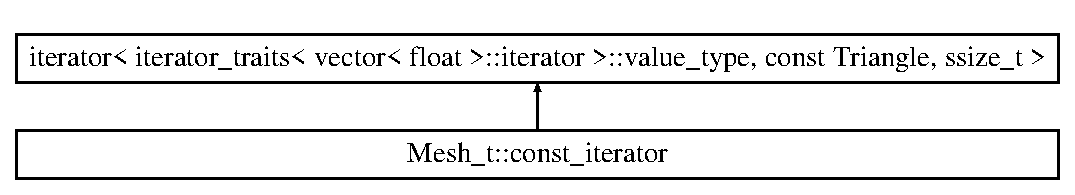
\includegraphics[height=2.000000cm]{classMesh__t_1_1const__iterator}
\end{center}
\end{figure}
\subsection*{Public Member Functions}
\begin{DoxyCompactItemize}
\item 
\hyperlink{classMesh__t_1_1const__iterator_a12b40b43154b6bed604ee50cf9baa7b6}{const\+\_\+iterator} ()
\begin{DoxyCompactList}\small\item\em Write what the function does here. \end{DoxyCompactList}\item 
bool \hyperlink{classMesh__t_1_1const__iterator_a9f420a6682f245fe125134ff77c79ceb}{operator==} (const \hyperlink{classMesh__t_1_1const__iterator}{const\+\_\+iterator} \&rt) const 
\begin{DoxyCompactList}\small\item\em Write what the function does here. \end{DoxyCompactList}\item 
bool \hyperlink{classMesh__t_1_1const__iterator_aef0e8e475e9ebc4ed2d8312686a65494}{operator!=} (const \hyperlink{classMesh__t_1_1const__iterator}{const\+\_\+iterator} \&rt) const 
\begin{DoxyCompactList}\small\item\em Write what the function does here. \end{DoxyCompactList}\item 
const \hyperlink{structTriangle}{Triangle} \& \hyperlink{classMesh__t_1_1const__iterator_a350801d9318c796df45dc627cfae3030}{operator$\ast$} () const 
\begin{DoxyCompactList}\small\item\em Write what the function does here. \end{DoxyCompactList}\item 
const \hyperlink{structTriangle}{Triangle} \& \hyperlink{classMesh__t_1_1const__iterator_aff99bf979efd14f19f7a5689bae8f387}{operator\mbox{[}$\,$\mbox{]}} (ssize\+\_\+t index) const 
\begin{DoxyCompactList}\small\item\em Write what the function does here. \end{DoxyCompactList}\item 
const \hyperlink{structTriangle}{Triangle} $\ast$ \hyperlink{classMesh__t_1_1const__iterator_a839942103e8fcba845e817f6b1247068}{operator-\/$>$} () const 
\begin{DoxyCompactList}\small\item\em Write what the function does here. \end{DoxyCompactList}\item 
\hyperlink{classMesh__t_1_1const__iterator}{const\+\_\+iterator} \hyperlink{classMesh__t_1_1const__iterator_aec122ec9ac2784f2bfb25edd9312486a}{operator+} (ssize\+\_\+t i) const 
\begin{DoxyCompactList}\small\item\em Write what the function does here. \end{DoxyCompactList}\item 
\hyperlink{classMesh__t_1_1const__iterator}{const\+\_\+iterator} \hyperlink{classMesh__t_1_1const__iterator_abb246af63c0fe9bda59bfbf3af590e43}{operator-\/} (ssize\+\_\+t i) const 
\begin{DoxyCompactList}\small\item\em Write what the function does here. \end{DoxyCompactList}\item 
ssize\+\_\+t \hyperlink{classMesh__t_1_1const__iterator_a1278d4a60a6ab8d6a1dfd0fd86ed2f5b}{operator-\/} (const \hyperlink{classMesh__t_1_1const__iterator}{const\+\_\+iterator} \&r) const 
\begin{DoxyCompactList}\small\item\em Write what the function does here. \end{DoxyCompactList}\item 
const \hyperlink{classMesh__t_1_1const__iterator}{const\+\_\+iterator} \& \hyperlink{classMesh__t_1_1const__iterator_a4cbe8dca9e1cbf5224de5acd0c130366}{operator+=} (ssize\+\_\+t i)
\begin{DoxyCompactList}\small\item\em Write what the function does here. \end{DoxyCompactList}\item 
const \hyperlink{classMesh__t_1_1const__iterator}{const\+\_\+iterator} \& \hyperlink{classMesh__t_1_1const__iterator_a2c01055aeeea1bba07f0303d7d89f5dc}{operator-\/=} (ssize\+\_\+t i)
\begin{DoxyCompactList}\small\item\em Write what the function does here. \end{DoxyCompactList}\item 
const \hyperlink{classMesh__t_1_1const__iterator}{const\+\_\+iterator} \& \hyperlink{classMesh__t_1_1const__iterator_a579d9d6186ddaba92c4f2d96f9783cd2}{operator++} ()
\begin{DoxyCompactList}\small\item\em Write what the function does here. \end{DoxyCompactList}\item 
const \hyperlink{classMesh__t_1_1const__iterator}{const\+\_\+iterator} \& \hyperlink{classMesh__t_1_1const__iterator_ab0bb21309502c144e73cd4a4669632f9}{operator-\/-\/} ()
\begin{DoxyCompactList}\small\item\em Write what the function does here. \end{DoxyCompactList}\item 
\hyperlink{classMesh__t_1_1const__iterator}{const\+\_\+iterator} \hyperlink{classMesh__t_1_1const__iterator_ae4dfd51c231b4aca1ccd37af446452bc}{operator++} (int)
\begin{DoxyCompactList}\small\item\em Write what the function does here. \end{DoxyCompactList}\item 
\hyperlink{classMesh__t_1_1const__iterator}{const\+\_\+iterator} \hyperlink{classMesh__t_1_1const__iterator_a55ba9083411021658f0f226773f97b09}{operator-\/-\/} (int)
\begin{DoxyCompactList}\small\item\em Write what the function does here. \end{DoxyCompactList}\item 
bool \hyperlink{classMesh__t_1_1const__iterator_a070ce17271dafc69c4de9f231bd667da}{operator$>$} (const \hyperlink{classMesh__t_1_1const__iterator}{const\+\_\+iterator} \&r) const 
\begin{DoxyCompactList}\small\item\em Write what the function does here. \end{DoxyCompactList}\item 
bool \hyperlink{classMesh__t_1_1const__iterator_a376992b96fd309bce6335e4ad4c564f7}{operator$>$=} (const \hyperlink{classMesh__t_1_1const__iterator}{const\+\_\+iterator} \&r) const 
\begin{DoxyCompactList}\small\item\em Write what the function does here. \end{DoxyCompactList}\item 
bool \hyperlink{classMesh__t_1_1const__iterator_ab072053e0d01075225a883405e5e6953}{operator$<$} (const \hyperlink{classMesh__t_1_1const__iterator}{const\+\_\+iterator} \&r) const 
\begin{DoxyCompactList}\small\item\em Write what the function does here. \end{DoxyCompactList}\item 
bool \hyperlink{classMesh__t_1_1const__iterator_a6ed80538dc270a480f24efeca60a2c39}{operator$<$=} (const \hyperlink{classMesh__t_1_1const__iterator}{const\+\_\+iterator} \&r) const 
\begin{DoxyCompactList}\small\item\em Write what the function does here. \end{DoxyCompactList}\end{DoxyCompactItemize}
\subsection*{Private Types}
\begin{DoxyCompactItemize}
\item 
\hypertarget{classMesh__t_1_1const__iterator_a2b700a6a28c6afcf4573ad39077cb24c}{typedef vector$<$ float $>$\\*
\+::\hyperlink{classMesh__t_1_1const__iterator}{const\+\_\+iterator} {\bfseries sub\+Iterator}}\label{classMesh__t_1_1const__iterator_a2b700a6a28c6afcf4573ad39077cb24c}

\end{DoxyCompactItemize}
\subsection*{Private Member Functions}
\begin{DoxyCompactItemize}
\item 
\hypertarget{classMesh__t_1_1const__iterator_a26e718515dda633e3681a1d4659e35b6}{{\bfseries const\+\_\+iterator} (sub\+Iterator point\+Iterator, sub\+Iterator color\+Iterator, sub\+Iterator texture\+Coord\+Iterator)}\label{classMesh__t_1_1const__iterator_a26e718515dda633e3681a1d4659e35b6}

\end{DoxyCompactItemize}
\subsection*{Private Attributes}
\begin{DoxyCompactItemize}
\item 
\hypertarget{classMesh__t_1_1const__iterator_aa0ff7c5e1b1f15e37f6bf47ae48813bc}{\hyperlink{structTriangle}{Triangle} {\bfseries tri}}\label{classMesh__t_1_1const__iterator_aa0ff7c5e1b1f15e37f6bf47ae48813bc}

\item 
\hypertarget{classMesh__t_1_1const__iterator_a956eff916034727260807fc25547ad26}{sub\+Iterator {\bfseries point\+Iterator}}\label{classMesh__t_1_1const__iterator_a956eff916034727260807fc25547ad26}

\item 
\hypertarget{classMesh__t_1_1const__iterator_ac96c04ebda6b049fc2cf54662998760a}{sub\+Iterator {\bfseries color\+Iterator}}\label{classMesh__t_1_1const__iterator_ac96c04ebda6b049fc2cf54662998760a}

\item 
\hypertarget{classMesh__t_1_1const__iterator_a995d3fea982ee9db95e52ac52eba1629}{sub\+Iterator {\bfseries texture\+Coord\+Iterator}}\label{classMesh__t_1_1const__iterator_a995d3fea982ee9db95e52ac52eba1629}

\end{DoxyCompactItemize}
\subsection*{Friends}
\begin{DoxyCompactItemize}
\item 
\hypertarget{classMesh__t_1_1const__iterator_a84c47c5327343f1dfe4c78205c3d2941}{class {\bfseries Mesh\+\_\+t}}\label{classMesh__t_1_1const__iterator_a84c47c5327343f1dfe4c78205c3d2941}

\item 
\hyperlink{classMesh__t_1_1const__iterator}{const\+\_\+iterator} \hyperlink{classMesh__t_1_1const__iterator_ad74c50fdf0b856c3b675b50670526fc8}{operator+} (ssize\+\_\+t i, const \hyperlink{classMesh__t_1_1const__iterator}{const\+\_\+iterator} \&iter)
\begin{DoxyCompactList}\small\item\em Write what the function does here. \end{DoxyCompactList}\end{DoxyCompactItemize}


\subsection{Detailed Description}
Write what the function does here. 


\begin{DoxyParams}{Parameters}
{\em value\+\_\+type} & \\
\hline
{\em \hyperlink{structTriangle}{Triangle}} & \\
\hline
\end{DoxyParams}

\begin{DoxyRetVals}{Return values}
{\em (variable)} & (description of variable) \\
\hline
\end{DoxyRetVals}


Definition at line 442 of file mesh.\+h.



\subsection{Constructor \& Destructor Documentation}
\hypertarget{classMesh__t_1_1const__iterator_a12b40b43154b6bed604ee50cf9baa7b6}{\index{Mesh\+\_\+t\+::const\+\_\+iterator@{Mesh\+\_\+t\+::const\+\_\+iterator}!const\+\_\+iterator@{const\+\_\+iterator}}
\index{const\+\_\+iterator@{const\+\_\+iterator}!Mesh\+\_\+t\+::const\+\_\+iterator@{Mesh\+\_\+t\+::const\+\_\+iterator}}
\subsubsection[{const\+\_\+iterator}]{\setlength{\rightskip}{0pt plus 5cm}Mesh\+\_\+t\+::const\+\_\+iterator\+::const\+\_\+iterator (
\begin{DoxyParamCaption}
{}
\end{DoxyParamCaption}
)\hspace{0.3cm}{\ttfamily [inline]}}}\label{classMesh__t_1_1const__iterator_a12b40b43154b6bed604ee50cf9baa7b6}


Write what the function does here. 


\begin{DoxyRetVals}{Return values}
{\em (variable)} & (description of variable) \\
\hline
\end{DoxyRetVals}


Definition at line 460 of file mesh.\+h.



Referenced by operator+().


\begin{DoxyCode}
461         \{
462         \}
\end{DoxyCode}


\subsection{Member Function Documentation}
\hypertarget{classMesh__t_1_1const__iterator_aef0e8e475e9ebc4ed2d8312686a65494}{\index{Mesh\+\_\+t\+::const\+\_\+iterator@{Mesh\+\_\+t\+::const\+\_\+iterator}!operator"!=@{operator"!=}}
\index{operator"!=@{operator"!=}!Mesh\+\_\+t\+::const\+\_\+iterator@{Mesh\+\_\+t\+::const\+\_\+iterator}}
\subsubsection[{operator"!=}]{\setlength{\rightskip}{0pt plus 5cm}bool Mesh\+\_\+t\+::const\+\_\+iterator\+::operator!= (
\begin{DoxyParamCaption}
\item[{const {\bf const\+\_\+iterator} \&}]{rt}
\end{DoxyParamCaption}
) const\hspace{0.3cm}{\ttfamily [inline]}}}\label{classMesh__t_1_1const__iterator_aef0e8e475e9ebc4ed2d8312686a65494}


Write what the function does here. 


\begin{DoxyParams}{Parameters}
{\em rt} & \\
\hline
\end{DoxyParams}

\begin{DoxyRetVals}{Return values}
{\em (variable)} & (description of variable) \\
\hline
\end{DoxyRetVals}


Definition at line 483 of file mesh.\+h.


\begin{DoxyCode}
484         \{
485             \textcolor{keywordflow}{return} pointIterator != rt.pointIterator;
486         \}
\end{DoxyCode}
\hypertarget{classMesh__t_1_1const__iterator_a350801d9318c796df45dc627cfae3030}{\index{Mesh\+\_\+t\+::const\+\_\+iterator@{Mesh\+\_\+t\+::const\+\_\+iterator}!operator$\ast$@{operator$\ast$}}
\index{operator$\ast$@{operator$\ast$}!Mesh\+\_\+t\+::const\+\_\+iterator@{Mesh\+\_\+t\+::const\+\_\+iterator}}
\subsubsection[{operator$\ast$}]{\setlength{\rightskip}{0pt plus 5cm}const {\bf Triangle}\& Mesh\+\_\+t\+::const\+\_\+iterator\+::operator$\ast$ (
\begin{DoxyParamCaption}
{}
\end{DoxyParamCaption}
) const\hspace{0.3cm}{\ttfamily [inline]}}}\label{classMesh__t_1_1const__iterator_a350801d9318c796df45dc627cfae3030}


Write what the function does here. 


\begin{DoxyRetVals}{Return values}
{\em (variable)} & (description of variable) \\
\hline
\end{DoxyRetVals}


Definition at line 493 of file mesh.\+h.



Referenced by operator-\/$>$().


\begin{DoxyCode}
494         \{
495             subIterator p = pointIterator, c = colorIterator, t = textureCoordIterator;
496             tri.p[0] = \hyperlink{structVectorF}{VectorF}(p[0], p[1], p[2]);
497             tri.p[1] = \hyperlink{structVectorF}{VectorF}(p[3], p[4], p[5]);
498             tri.p[2] = \hyperlink{structVectorF}{VectorF}(p[6], p[7], p[8]);
499             tri.c[0] = \hyperlink{structColor}{Color}(c[0], c[1], c[2], c[3]);
500             tri.c[1] = \hyperlink{structColor}{Color}(c[4], c[5], c[6], c[7]);
501             tri.c[2] = \hyperlink{structColor}{Color}(c[8], c[9], c[10], c[11]);
502             tri.t[0] = \hyperlink{structTextureCoord}{TextureCoord}(t[0], t[1]);
503             tri.t[1] = \hyperlink{structTextureCoord}{TextureCoord}(t[2], t[3]);
504             tri.t[2] = \hyperlink{structTextureCoord}{TextureCoord}(t[4], t[5]);
505             \textcolor{keywordflow}{return} tri;
506         \}
\end{DoxyCode}
\hypertarget{classMesh__t_1_1const__iterator_aec122ec9ac2784f2bfb25edd9312486a}{\index{Mesh\+\_\+t\+::const\+\_\+iterator@{Mesh\+\_\+t\+::const\+\_\+iterator}!operator+@{operator+}}
\index{operator+@{operator+}!Mesh\+\_\+t\+::const\+\_\+iterator@{Mesh\+\_\+t\+::const\+\_\+iterator}}
\subsubsection[{operator+}]{\setlength{\rightskip}{0pt plus 5cm}{\bf const\+\_\+iterator} Mesh\+\_\+t\+::const\+\_\+iterator\+::operator+ (
\begin{DoxyParamCaption}
\item[{ssize\+\_\+t}]{i}
\end{DoxyParamCaption}
) const\hspace{0.3cm}{\ttfamily [inline]}}}\label{classMesh__t_1_1const__iterator_aec122ec9ac2784f2bfb25edd9312486a}


Write what the function does here. 


\begin{DoxyParams}{Parameters}
{\em i} & \\
\hline
\end{DoxyParams}

\begin{DoxyRetVals}{Return values}
{\em (variable)} & (description of variable) \\
\hline
\end{DoxyRetVals}


Definition at line 537 of file mesh.\+h.



References const\+\_\+iterator().



Referenced by operator+=(), operator-\/(), and operator\mbox{[}$\,$\mbox{]}().


\begin{DoxyCode}
538         \{
539             \textcolor{keywordflow}{return} \hyperlink{classMesh__t_1_1const__iterator_a12b40b43154b6bed604ee50cf9baa7b6}{const\_iterator}(pointIterator + i * floatsPerPoint * pointsPerTriangle,
540                     colorIterator + i * floatsPerColor * colorsPerTriangle,
541                     textureCoordIterator + i * floatsPerTextureCoord * textureCoordsPerTriangle);
542         \}
\end{DoxyCode}
\hypertarget{classMesh__t_1_1const__iterator_a579d9d6186ddaba92c4f2d96f9783cd2}{\index{Mesh\+\_\+t\+::const\+\_\+iterator@{Mesh\+\_\+t\+::const\+\_\+iterator}!operator++@{operator++}}
\index{operator++@{operator++}!Mesh\+\_\+t\+::const\+\_\+iterator@{Mesh\+\_\+t\+::const\+\_\+iterator}}
\subsubsection[{operator++}]{\setlength{\rightskip}{0pt plus 5cm}const {\bf const\+\_\+iterator}\& Mesh\+\_\+t\+::const\+\_\+iterator\+::operator++ (
\begin{DoxyParamCaption}
{}
\end{DoxyParamCaption}
)\hspace{0.3cm}{\ttfamily [inline]}}}\label{classMesh__t_1_1const__iterator_a579d9d6186ddaba92c4f2d96f9783cd2}


Write what the function does here. 


\begin{DoxyRetVals}{Return values}
{\em (variable)} & (description of variable) \\
\hline
\end{DoxyRetVals}


Definition at line 610 of file mesh.\+h.



References operator+=().



Referenced by operator++().


\begin{DoxyCode}
611         \{
612             \textcolor{keywordflow}{return} \hyperlink{classMesh__t_1_1const__iterator_a4cbe8dca9e1cbf5224de5acd0c130366}{operator +=}(1);
613         \}
\end{DoxyCode}
\hypertarget{classMesh__t_1_1const__iterator_ae4dfd51c231b4aca1ccd37af446452bc}{\index{Mesh\+\_\+t\+::const\+\_\+iterator@{Mesh\+\_\+t\+::const\+\_\+iterator}!operator++@{operator++}}
\index{operator++@{operator++}!Mesh\+\_\+t\+::const\+\_\+iterator@{Mesh\+\_\+t\+::const\+\_\+iterator}}
\subsubsection[{operator++}]{\setlength{\rightskip}{0pt plus 5cm}{\bf const\+\_\+iterator} Mesh\+\_\+t\+::const\+\_\+iterator\+::operator++ (
\begin{DoxyParamCaption}
\item[{int}]{}
\end{DoxyParamCaption}
)\hspace{0.3cm}{\ttfamily [inline]}}}\label{classMesh__t_1_1const__iterator_ae4dfd51c231b4aca1ccd37af446452bc}


Write what the function does here. 


\begin{DoxyParams}{Parameters}
{\em int} & \\
\hline
\end{DoxyParams}

\begin{DoxyRetVals}{Return values}
{\em (variable)} & (description of variable) \\
\hline
\end{DoxyRetVals}


Definition at line 632 of file mesh.\+h.



References operator++().


\begin{DoxyCode}
633         \{
634             \hyperlink{classMesh__t_1_1const__iterator_a12b40b43154b6bed604ee50cf9baa7b6}{const\_iterator} retval = *\textcolor{keyword}{this};
635             \hyperlink{classMesh__t_1_1const__iterator_a579d9d6186ddaba92c4f2d96f9783cd2}{operator ++}();
636             \textcolor{keywordflow}{return} retval;
637         \}
\end{DoxyCode}
\hypertarget{classMesh__t_1_1const__iterator_a4cbe8dca9e1cbf5224de5acd0c130366}{\index{Mesh\+\_\+t\+::const\+\_\+iterator@{Mesh\+\_\+t\+::const\+\_\+iterator}!operator+=@{operator+=}}
\index{operator+=@{operator+=}!Mesh\+\_\+t\+::const\+\_\+iterator@{Mesh\+\_\+t\+::const\+\_\+iterator}}
\subsubsection[{operator+=}]{\setlength{\rightskip}{0pt plus 5cm}const {\bf const\+\_\+iterator}\& Mesh\+\_\+t\+::const\+\_\+iterator\+::operator+= (
\begin{DoxyParamCaption}
\item[{ssize\+\_\+t}]{i}
\end{DoxyParamCaption}
)\hspace{0.3cm}{\ttfamily [inline]}}}\label{classMesh__t_1_1const__iterator_a4cbe8dca9e1cbf5224de5acd0c130366}


Write what the function does here. 


\begin{DoxyParams}{Parameters}
{\em i} & \\
\hline
\end{DoxyParams}

\begin{DoxyRetVals}{Return values}
{\em (variable)} & (description of variable) \\
\hline
\end{DoxyRetVals}


Definition at line 588 of file mesh.\+h.



References operator+().



Referenced by operator++().


\begin{DoxyCode}
589         \{
590             \textcolor{keywordflow}{return} *\textcolor{keyword}{this} = \hyperlink{classMesh__t_1_1const__iterator_aec122ec9ac2784f2bfb25edd9312486a}{operator +}(i);
591         \}
\end{DoxyCode}
\hypertarget{classMesh__t_1_1const__iterator_abb246af63c0fe9bda59bfbf3af590e43}{\index{Mesh\+\_\+t\+::const\+\_\+iterator@{Mesh\+\_\+t\+::const\+\_\+iterator}!operator-\/@{operator-\/}}
\index{operator-\/@{operator-\/}!Mesh\+\_\+t\+::const\+\_\+iterator@{Mesh\+\_\+t\+::const\+\_\+iterator}}
\subsubsection[{operator-\/}]{\setlength{\rightskip}{0pt plus 5cm}{\bf const\+\_\+iterator} Mesh\+\_\+t\+::const\+\_\+iterator\+::operator-\/ (
\begin{DoxyParamCaption}
\item[{ssize\+\_\+t}]{i}
\end{DoxyParamCaption}
) const\hspace{0.3cm}{\ttfamily [inline]}}}\label{classMesh__t_1_1const__iterator_abb246af63c0fe9bda59bfbf3af590e43}


Write what the function does here. 


\begin{DoxyParams}{Parameters}
{\em i} & \\
\hline
\end{DoxyParams}

\begin{DoxyRetVals}{Return values}
{\em (variable)} & (description of variable) \\
\hline
\end{DoxyRetVals}


Definition at line 564 of file mesh.\+h.



References operator+().



Referenced by operator-\/=().


\begin{DoxyCode}
565         \{
566             \textcolor{keywordflow}{return} \hyperlink{classMesh__t_1_1const__iterator_aec122ec9ac2784f2bfb25edd9312486a}{operator +}(-i);
567         \}
\end{DoxyCode}
\hypertarget{classMesh__t_1_1const__iterator_a1278d4a60a6ab8d6a1dfd0fd86ed2f5b}{\index{Mesh\+\_\+t\+::const\+\_\+iterator@{Mesh\+\_\+t\+::const\+\_\+iterator}!operator-\/@{operator-\/}}
\index{operator-\/@{operator-\/}!Mesh\+\_\+t\+::const\+\_\+iterator@{Mesh\+\_\+t\+::const\+\_\+iterator}}
\subsubsection[{operator-\/}]{\setlength{\rightskip}{0pt plus 5cm}ssize\+\_\+t Mesh\+\_\+t\+::const\+\_\+iterator\+::operator-\/ (
\begin{DoxyParamCaption}
\item[{const {\bf const\+\_\+iterator} \&}]{r}
\end{DoxyParamCaption}
) const\hspace{0.3cm}{\ttfamily [inline]}}}\label{classMesh__t_1_1const__iterator_a1278d4a60a6ab8d6a1dfd0fd86ed2f5b}


Write what the function does here. 


\begin{DoxyParams}{Parameters}
{\em r} & \\
\hline
\end{DoxyParams}

\begin{DoxyRetVals}{Return values}
{\em (variable)} & (description of variable) \\
\hline
\end{DoxyRetVals}


Definition at line 576 of file mesh.\+h.


\begin{DoxyCode}
577         \{
578             \textcolor{keywordflow}{return} (textureCoordIterator - r.textureCoordIterator) / (floatsPerTextureCoord * 
      textureCoordsPerTriangle);
579         \}
\end{DoxyCode}
\hypertarget{classMesh__t_1_1const__iterator_ab0bb21309502c144e73cd4a4669632f9}{\index{Mesh\+\_\+t\+::const\+\_\+iterator@{Mesh\+\_\+t\+::const\+\_\+iterator}!operator-\/-\/@{operator-\/-\/}}
\index{operator-\/-\/@{operator-\/-\/}!Mesh\+\_\+t\+::const\+\_\+iterator@{Mesh\+\_\+t\+::const\+\_\+iterator}}
\subsubsection[{operator-\/-\/}]{\setlength{\rightskip}{0pt plus 5cm}const {\bf const\+\_\+iterator}\& Mesh\+\_\+t\+::const\+\_\+iterator\+::operator-\/-\/ (
\begin{DoxyParamCaption}
{}
\end{DoxyParamCaption}
)\hspace{0.3cm}{\ttfamily [inline]}}}\label{classMesh__t_1_1const__iterator_ab0bb21309502c144e73cd4a4669632f9}


Write what the function does here. 


\begin{DoxyRetVals}{Return values}
{\em (variable)} & (description of variable) \\
\hline
\end{DoxyRetVals}


Definition at line 620 of file mesh.\+h.



References operator-\/=().



Referenced by operator-\/-\/().


\begin{DoxyCode}
621         \{
622             \textcolor{keywordflow}{return} \hyperlink{classMesh__t_1_1const__iterator_a2c01055aeeea1bba07f0303d7d89f5dc}{operator -=}(1);
623         \}
\end{DoxyCode}
\hypertarget{classMesh__t_1_1const__iterator_a55ba9083411021658f0f226773f97b09}{\index{Mesh\+\_\+t\+::const\+\_\+iterator@{Mesh\+\_\+t\+::const\+\_\+iterator}!operator-\/-\/@{operator-\/-\/}}
\index{operator-\/-\/@{operator-\/-\/}!Mesh\+\_\+t\+::const\+\_\+iterator@{Mesh\+\_\+t\+::const\+\_\+iterator}}
\subsubsection[{operator-\/-\/}]{\setlength{\rightskip}{0pt plus 5cm}{\bf const\+\_\+iterator} Mesh\+\_\+t\+::const\+\_\+iterator\+::operator-\/-\/ (
\begin{DoxyParamCaption}
\item[{int}]{}
\end{DoxyParamCaption}
)\hspace{0.3cm}{\ttfamily [inline]}}}\label{classMesh__t_1_1const__iterator_a55ba9083411021658f0f226773f97b09}


Write what the function does here. 


\begin{DoxyParams}{Parameters}
{\em int} & \\
\hline
\end{DoxyParams}

\begin{DoxyRetVals}{Return values}
{\em (variable)} & (description of variable) \\
\hline
\end{DoxyRetVals}


Definition at line 646 of file mesh.\+h.



References operator-\/-\/().


\begin{DoxyCode}
647         \{
648             \hyperlink{classMesh__t_1_1const__iterator_a12b40b43154b6bed604ee50cf9baa7b6}{const\_iterator} retval = *\textcolor{keyword}{this};
649             \hyperlink{classMesh__t_1_1const__iterator_ab0bb21309502c144e73cd4a4669632f9}{operator --}();
650             \textcolor{keywordflow}{return} retval;
651         \}
\end{DoxyCode}
\hypertarget{classMesh__t_1_1const__iterator_a2c01055aeeea1bba07f0303d7d89f5dc}{\index{Mesh\+\_\+t\+::const\+\_\+iterator@{Mesh\+\_\+t\+::const\+\_\+iterator}!operator-\/=@{operator-\/=}}
\index{operator-\/=@{operator-\/=}!Mesh\+\_\+t\+::const\+\_\+iterator@{Mesh\+\_\+t\+::const\+\_\+iterator}}
\subsubsection[{operator-\/=}]{\setlength{\rightskip}{0pt plus 5cm}const {\bf const\+\_\+iterator}\& Mesh\+\_\+t\+::const\+\_\+iterator\+::operator-\/= (
\begin{DoxyParamCaption}
\item[{ssize\+\_\+t}]{i}
\end{DoxyParamCaption}
)\hspace{0.3cm}{\ttfamily [inline]}}}\label{classMesh__t_1_1const__iterator_a2c01055aeeea1bba07f0303d7d89f5dc}


Write what the function does here. 


\begin{DoxyParams}{Parameters}
{\em i} & \\
\hline
\end{DoxyParams}

\begin{DoxyRetVals}{Return values}
{\em (variable)} & (description of variable) \\
\hline
\end{DoxyRetVals}


Definition at line 600 of file mesh.\+h.



References operator-\/().



Referenced by operator-\/-\/().


\begin{DoxyCode}
601         \{
602             \textcolor{keywordflow}{return} *\textcolor{keyword}{this} = \hyperlink{classMesh__t_1_1const__iterator_abb246af63c0fe9bda59bfbf3af590e43}{operator -}(i);
603         \}
\end{DoxyCode}
\hypertarget{classMesh__t_1_1const__iterator_a839942103e8fcba845e817f6b1247068}{\index{Mesh\+\_\+t\+::const\+\_\+iterator@{Mesh\+\_\+t\+::const\+\_\+iterator}!operator-\/$>$@{operator-\/$>$}}
\index{operator-\/$>$@{operator-\/$>$}!Mesh\+\_\+t\+::const\+\_\+iterator@{Mesh\+\_\+t\+::const\+\_\+iterator}}
\subsubsection[{operator-\/$>$}]{\setlength{\rightskip}{0pt plus 5cm}const {\bf Triangle}$\ast$ Mesh\+\_\+t\+::const\+\_\+iterator\+::operator-\/$>$ (
\begin{DoxyParamCaption}
{}
\end{DoxyParamCaption}
) const\hspace{0.3cm}{\ttfamily [inline]}}}\label{classMesh__t_1_1const__iterator_a839942103e8fcba845e817f6b1247068}


Write what the function does here. 


\begin{DoxyRetVals}{Return values}
{\em (variable)} & (description of variable) \\
\hline
\end{DoxyRetVals}


Definition at line 525 of file mesh.\+h.



References operator$\ast$().


\begin{DoxyCode}
526         \{
527             \textcolor{keywordflow}{return} &\hyperlink{classMesh__t_1_1const__iterator_a350801d9318c796df45dc627cfae3030}{operator *}();
528         \}
\end{DoxyCode}
\hypertarget{classMesh__t_1_1const__iterator_ab072053e0d01075225a883405e5e6953}{\index{Mesh\+\_\+t\+::const\+\_\+iterator@{Mesh\+\_\+t\+::const\+\_\+iterator}!operator$<$@{operator$<$}}
\index{operator$<$@{operator$<$}!Mesh\+\_\+t\+::const\+\_\+iterator@{Mesh\+\_\+t\+::const\+\_\+iterator}}
\subsubsection[{operator$<$}]{\setlength{\rightskip}{0pt plus 5cm}bool Mesh\+\_\+t\+::const\+\_\+iterator\+::operator$<$ (
\begin{DoxyParamCaption}
\item[{const {\bf const\+\_\+iterator} \&}]{r}
\end{DoxyParamCaption}
) const\hspace{0.3cm}{\ttfamily [inline]}}}\label{classMesh__t_1_1const__iterator_ab072053e0d01075225a883405e5e6953}


Write what the function does here. 


\begin{DoxyParams}{Parameters}
{\em r} & \\
\hline
\end{DoxyParams}

\begin{DoxyRetVals}{Return values}
{\em (variable)} & (description of variable) \\
\hline
\end{DoxyRetVals}


Definition at line 684 of file mesh.\+h.


\begin{DoxyCode}
685         \{
686             \textcolor{keywordflow}{return} pointIterator < r.pointIterator;
687         \}
\end{DoxyCode}
\hypertarget{classMesh__t_1_1const__iterator_a6ed80538dc270a480f24efeca60a2c39}{\index{Mesh\+\_\+t\+::const\+\_\+iterator@{Mesh\+\_\+t\+::const\+\_\+iterator}!operator$<$=@{operator$<$=}}
\index{operator$<$=@{operator$<$=}!Mesh\+\_\+t\+::const\+\_\+iterator@{Mesh\+\_\+t\+::const\+\_\+iterator}}
\subsubsection[{operator$<$=}]{\setlength{\rightskip}{0pt plus 5cm}bool Mesh\+\_\+t\+::const\+\_\+iterator\+::operator$<$= (
\begin{DoxyParamCaption}
\item[{const {\bf const\+\_\+iterator} \&}]{r}
\end{DoxyParamCaption}
) const\hspace{0.3cm}{\ttfamily [inline]}}}\label{classMesh__t_1_1const__iterator_a6ed80538dc270a480f24efeca60a2c39}


Write what the function does here. 


\begin{DoxyParams}{Parameters}
{\em r} & \\
\hline
\end{DoxyParams}

\begin{DoxyRetVals}{Return values}
{\em (variable)} & (description of variable) \\
\hline
\end{DoxyRetVals}


Definition at line 696 of file mesh.\+h.


\begin{DoxyCode}
697         \{
698             \textcolor{keywordflow}{return} pointIterator <= r.pointIterator;
699         \}
\end{DoxyCode}
\hypertarget{classMesh__t_1_1const__iterator_a9f420a6682f245fe125134ff77c79ceb}{\index{Mesh\+\_\+t\+::const\+\_\+iterator@{Mesh\+\_\+t\+::const\+\_\+iterator}!operator==@{operator==}}
\index{operator==@{operator==}!Mesh\+\_\+t\+::const\+\_\+iterator@{Mesh\+\_\+t\+::const\+\_\+iterator}}
\subsubsection[{operator==}]{\setlength{\rightskip}{0pt plus 5cm}bool Mesh\+\_\+t\+::const\+\_\+iterator\+::operator== (
\begin{DoxyParamCaption}
\item[{const {\bf const\+\_\+iterator} \&}]{rt}
\end{DoxyParamCaption}
) const\hspace{0.3cm}{\ttfamily [inline]}}}\label{classMesh__t_1_1const__iterator_a9f420a6682f245fe125134ff77c79ceb}


Write what the function does here. 


\begin{DoxyParams}{Parameters}
{\em rt} & \\
\hline
\end{DoxyParams}

\begin{DoxyRetVals}{Return values}
{\em (variable)} & (description of variable) \\
\hline
\end{DoxyRetVals}


Definition at line 471 of file mesh.\+h.


\begin{DoxyCode}
472         \{
473             \textcolor{keywordflow}{return} pointIterator == rt.pointIterator;
474         \}
\end{DoxyCode}
\hypertarget{classMesh__t_1_1const__iterator_a070ce17271dafc69c4de9f231bd667da}{\index{Mesh\+\_\+t\+::const\+\_\+iterator@{Mesh\+\_\+t\+::const\+\_\+iterator}!operator$>$@{operator$>$}}
\index{operator$>$@{operator$>$}!Mesh\+\_\+t\+::const\+\_\+iterator@{Mesh\+\_\+t\+::const\+\_\+iterator}}
\subsubsection[{operator$>$}]{\setlength{\rightskip}{0pt plus 5cm}bool Mesh\+\_\+t\+::const\+\_\+iterator\+::operator$>$ (
\begin{DoxyParamCaption}
\item[{const {\bf const\+\_\+iterator} \&}]{r}
\end{DoxyParamCaption}
) const\hspace{0.3cm}{\ttfamily [inline]}}}\label{classMesh__t_1_1const__iterator_a070ce17271dafc69c4de9f231bd667da}


Write what the function does here. 


\begin{DoxyParams}{Parameters}
{\em r} & \\
\hline
\end{DoxyParams}

\begin{DoxyRetVals}{Return values}
{\em (variable)} & (description of variable) \\
\hline
\end{DoxyRetVals}


Definition at line 660 of file mesh.\+h.


\begin{DoxyCode}
661         \{
662             \textcolor{keywordflow}{return} pointIterator > r.pointIterator;
663         \}
\end{DoxyCode}
\hypertarget{classMesh__t_1_1const__iterator_a376992b96fd309bce6335e4ad4c564f7}{\index{Mesh\+\_\+t\+::const\+\_\+iterator@{Mesh\+\_\+t\+::const\+\_\+iterator}!operator$>$=@{operator$>$=}}
\index{operator$>$=@{operator$>$=}!Mesh\+\_\+t\+::const\+\_\+iterator@{Mesh\+\_\+t\+::const\+\_\+iterator}}
\subsubsection[{operator$>$=}]{\setlength{\rightskip}{0pt plus 5cm}bool Mesh\+\_\+t\+::const\+\_\+iterator\+::operator$>$= (
\begin{DoxyParamCaption}
\item[{const {\bf const\+\_\+iterator} \&}]{r}
\end{DoxyParamCaption}
) const\hspace{0.3cm}{\ttfamily [inline]}}}\label{classMesh__t_1_1const__iterator_a376992b96fd309bce6335e4ad4c564f7}


Write what the function does here. 


\begin{DoxyParams}{Parameters}
{\em r} & \\
\hline
\end{DoxyParams}

\begin{DoxyRetVals}{Return values}
{\em (variable)} & (description of variable) \\
\hline
\end{DoxyRetVals}


Definition at line 672 of file mesh.\+h.


\begin{DoxyCode}
673         \{
674             \textcolor{keywordflow}{return} pointIterator >= r.pointIterator;
675         \}
\end{DoxyCode}
\hypertarget{classMesh__t_1_1const__iterator_aff99bf979efd14f19f7a5689bae8f387}{\index{Mesh\+\_\+t\+::const\+\_\+iterator@{Mesh\+\_\+t\+::const\+\_\+iterator}!operator\mbox{[}$\,$\mbox{]}@{operator[]}}
\index{operator\mbox{[}$\,$\mbox{]}@{operator[]}!Mesh\+\_\+t\+::const\+\_\+iterator@{Mesh\+\_\+t\+::const\+\_\+iterator}}
\subsubsection[{operator[]}]{\setlength{\rightskip}{0pt plus 5cm}const {\bf Triangle}\& Mesh\+\_\+t\+::const\+\_\+iterator\+::operator\mbox{[}$\,$\mbox{]} (
\begin{DoxyParamCaption}
\item[{ssize\+\_\+t}]{index}
\end{DoxyParamCaption}
) const\hspace{0.3cm}{\ttfamily [inline]}}}\label{classMesh__t_1_1const__iterator_aff99bf979efd14f19f7a5689bae8f387}


Write what the function does here. 


\begin{DoxyParams}{Parameters}
{\em index} & \\
\hline
\end{DoxyParams}

\begin{DoxyRetVals}{Return values}
{\em (variable)} & (description of variable) \\
\hline
\end{DoxyRetVals}


Definition at line 515 of file mesh.\+h.



References operator+().


\begin{DoxyCode}
516         \{
517             \textcolor{keywordflow}{return} \hyperlink{classMesh__t_1_1const__iterator_aec122ec9ac2784f2bfb25edd9312486a}{operator +}(index).operator * ();
518         \}
\end{DoxyCode}


\subsection{Friends And Related Function Documentation}
\hypertarget{classMesh__t_1_1const__iterator_ad74c50fdf0b856c3b675b50670526fc8}{\index{Mesh\+\_\+t\+::const\+\_\+iterator@{Mesh\+\_\+t\+::const\+\_\+iterator}!operator+@{operator+}}
\index{operator+@{operator+}!Mesh\+\_\+t\+::const\+\_\+iterator@{Mesh\+\_\+t\+::const\+\_\+iterator}}
\subsubsection[{operator+}]{\setlength{\rightskip}{0pt plus 5cm}{\bf const\+\_\+iterator} operator+ (
\begin{DoxyParamCaption}
\item[{ssize\+\_\+t}]{i, }
\item[{const {\bf const\+\_\+iterator} \&}]{iter}
\end{DoxyParamCaption}
)\hspace{0.3cm}{\ttfamily [friend]}}}\label{classMesh__t_1_1const__iterator_ad74c50fdf0b856c3b675b50670526fc8}


Write what the function does here. 


\begin{DoxyParams}{Parameters}
{\em i} & \\
\hline
{\em iter} & \\
\hline
\end{DoxyParams}

\begin{DoxyRetVals}{Return values}
{\em (variable)} & (description of variable) \\
\hline
\end{DoxyRetVals}


Definition at line 552 of file mesh.\+h.


\begin{DoxyCode}
553         \{
554             \textcolor{keywordflow}{return} iter.operator + (i);
555         \}
\end{DoxyCode}


The documentation for this class was generated from the following file\+:\begin{DoxyCompactItemize}
\item 
mesh.\+h\end{DoxyCompactItemize}

\hypertarget{structCoord}{\section{Coord Struct Reference}
\label{structCoord}\index{Coord@{Coord}}
}
\subsection*{Public Member Functions}
\begin{DoxyCompactItemize}
\item 
\hypertarget{structCoord_a31640ee494a7c77331cc56de54894301}{{\bfseries Coord} (int x, int y)}\label{structCoord_a31640ee494a7c77331cc56de54894301}

\item 
\hypertarget{structCoord_abb0834bf89a754b762ee1ef476d5d8ec}{bool {\bfseries operator==} (const \hyperlink{structCoord}{Coord} \&c) const }\label{structCoord_abb0834bf89a754b762ee1ef476d5d8ec}

\end{DoxyCompactItemize}
\subsection*{Public Attributes}
\begin{DoxyCompactItemize}
\item 
\hypertarget{structCoord_a696eaa744360fc791d0e3b331c549dbe}{int {\bfseries x}}\label{structCoord_a696eaa744360fc791d0e3b331c549dbe}

\item 
\hypertarget{structCoord_a214166cca70cef7dda9201689c3e81ab}{int {\bfseries y}}\label{structCoord_a214166cca70cef7dda9201689c3e81ab}

\end{DoxyCompactItemize}
\subsection*{Friends}
\begin{DoxyCompactItemize}
\item 
\hypertarget{structCoord_a3336e09424c5c7145f570643d05e0c44}{ostream \& {\bfseries operator$<$$<$} (ostream \&, const \hyperlink{structCoord}{Coord} \&)}\label{structCoord_a3336e09424c5c7145f570643d05e0c44}

\end{DoxyCompactItemize}


\subsection{Detailed Description}


Definition at line 17 of file structs.\+h.



The documentation for this struct was generated from the following file\+:\begin{DoxyCompactItemize}
\item 
headers/structs.\+h\end{DoxyCompactItemize}

\hypertarget{structCubicSpline}{\section{Cubic\+Spline Struct Reference}
\label{structCubicSpline}\index{Cubic\+Spline@{Cubic\+Spline}}
}


Write what the function does here.  




{\ttfamily \#include $<$cubicspline.\+h$>$}

\subsection*{Public Member Functions}
\begin{DoxyCompactItemize}
\item 
\hypertarget{structCubicSpline_ae9889650db27305852f896d03d3bd75c}{{\bfseries Cubic\+Spline} (\hyperlink{structVectorF}{Vector\+F} p0, \hyperlink{structVectorF}{Vector\+F} p1)}\label{structCubicSpline_ae9889650db27305852f896d03d3bd75c}

\item 
\hypertarget{structCubicSpline_a661fd0aed3df6744f52f5ba3872b9251}{{\bfseries Cubic\+Spline} (\hyperlink{structVectorF}{Vector\+F} p0, \hyperlink{structVectorF}{Vector\+F} p1, \hyperlink{structVectorF}{Vector\+F} dp0, \hyperlink{structVectorF}{Vector\+F} dp1)}\label{structCubicSpline_a661fd0aed3df6744f52f5ba3872b9251}

\item 
\hyperlink{structVectorF}{Vector\+F} \hyperlink{structCubicSpline_a87a1c29ab58b648430f45668067d7a1c}{get\+Constant} () const 
\begin{DoxyCompactList}\small\item\em Write what the function does here. \end{DoxyCompactList}\item 
\hyperlink{structVectorF}{Vector\+F} \hyperlink{structCubicSpline_ada872ef617b059ef68490e828bcdf181}{get\+Linear} () const 
\begin{DoxyCompactList}\small\item\em Write what the function does here. \end{DoxyCompactList}\item 
\hyperlink{structVectorF}{Vector\+F} \hyperlink{structCubicSpline_a7d5792ff1314032122cd342d0616a50f}{get\+Quadratic} () const 
\begin{DoxyCompactList}\small\item\em Write what the function does here. \end{DoxyCompactList}\item 
\hyperlink{structVectorF}{Vector\+F} \hyperlink{structCubicSpline_a156525e59dae0cac2a81cf34cb673c87}{get\+Cubic} () const 
\begin{DoxyCompactList}\small\item\em Write what the function does here. \end{DoxyCompactList}\item 
\hyperlink{structVectorF}{Vector\+F} \hyperlink{structCubicSpline_a6b5d7cf704ce35a9bce93d6faf53a4fe}{evaluate} (float t) const 
\begin{DoxyCompactList}\small\item\em Write what the function does here. \end{DoxyCompactList}\item 
\hypertarget{structCubicSpline_a17f53f7cb9b49caa80eff66097b57145}{bool {\bfseries intersects} (const \hyperlink{structCubicSpline}{Cubic\+Spline} \&rt, \hyperlink{structVectorF}{Vector\+F} ignore\+Axis=\hyperlink{structVectorF}{Vector\+F}(0, 0, 1)) const }\label{structCubicSpline_a17f53f7cb9b49caa80eff66097b57145}

\item 
\hyperlink{structCubicSpline}{Cubic\+Spline} \hyperlink{structCubicSpline_a9af4ede47352f7d8d38b520632b2bf3d}{sub\+Section} (float min\+T, float max\+T) const 
\begin{DoxyCompactList}\small\item\em returns true if the splines intersect each other when projected onto the plane with normal == ignore\+Axis \end{DoxyCompactList}\end{DoxyCompactItemize}
\subsection*{Static Public Member Functions}
\begin{DoxyCompactItemize}
\item 
\hypertarget{structCubicSpline_ab4f44a0380e5834289a60957baeaf822}{static Mesh {\bfseries render\+Spline\+List} (const vector$<$ \hyperlink{structCubicSpline}{Cubic\+Spline} $>$ \&splines, \hyperlink{structTextureDescriptor}{Texture\+Descriptor} texture, \hyperlink{structColor}{Color} color, float line\+Width)}\label{structCubicSpline_ab4f44a0380e5834289a60957baeaf822}

\end{DoxyCompactItemize}
\subsection*{Public Attributes}
\begin{DoxyCompactItemize}
\item 
\hypertarget{structCubicSpline_a84b61c539162fcfa38762e67261e3db6}{\hyperlink{structVectorF}{Vector\+F} {\bfseries p0}}\label{structCubicSpline_a84b61c539162fcfa38762e67261e3db6}

\item 
\hypertarget{structCubicSpline_a1bee668bf0240d7b70fc7f93638d253a}{\hyperlink{structVectorF}{Vector\+F} {\bfseries p1}}\label{structCubicSpline_a1bee668bf0240d7b70fc7f93638d253a}

\item 
\hypertarget{structCubicSpline_a5ebae554d5f1da3baa730d698d1667ff}{\hyperlink{structVectorF}{Vector\+F} {\bfseries dp0}}\label{structCubicSpline_a5ebae554d5f1da3baa730d698d1667ff}

\item 
\hypertarget{structCubicSpline_aeefcf5d9423158b97037640c26cf24f0}{\hyperlink{structVectorF}{Vector\+F} {\bfseries dp1}}\label{structCubicSpline_aeefcf5d9423158b97037640c26cf24f0}

\end{DoxyCompactItemize}


\subsection{Detailed Description}
Write what the function does here. 

\begin{DoxyReturn}{Returns}

\end{DoxyReturn}


Definition at line 14 of file cubicspline.\+h.



\subsection{Member Function Documentation}
\hypertarget{structCubicSpline_a6b5d7cf704ce35a9bce93d6faf53a4fe}{\index{Cubic\+Spline@{Cubic\+Spline}!evaluate@{evaluate}}
\index{evaluate@{evaluate}!Cubic\+Spline@{Cubic\+Spline}}
\subsubsection[{evaluate}]{\setlength{\rightskip}{0pt plus 5cm}{\bf Vector\+F} Cubic\+Spline\+::evaluate (
\begin{DoxyParamCaption}
\item[{float}]{t}
\end{DoxyParamCaption}
) const\hspace{0.3cm}{\ttfamily [inline]}}}\label{structCubicSpline_a6b5d7cf704ce35a9bce93d6faf53a4fe}


Write what the function does here. 


\begin{DoxyParams}{Parameters}
{\em t} & \\
\hline
\end{DoxyParams}
\begin{DoxyReturn}{Returns}

\end{DoxyReturn}


Definition at line 78 of file cubicspline.\+h.


\begin{DoxyCode}
79     \{
80         \textcolor{keywordflow}{return} t * t * t * \hyperlink{structCubicSpline_a156525e59dae0cac2a81cf34cb673c87}{getCubic}() + t * t * \hyperlink{structCubicSpline_a7d5792ff1314032122cd342d0616a50f}{getQuadratic}() + t * 
      \hyperlink{structCubicSpline_ada872ef617b059ef68490e828bcdf181}{getLinear}() + \hyperlink{structCubicSpline_a87a1c29ab58b648430f45668067d7a1c}{getConstant}();
81     \}
\end{DoxyCode}
\hypertarget{structCubicSpline_a87a1c29ab58b648430f45668067d7a1c}{\index{Cubic\+Spline@{Cubic\+Spline}!get\+Constant@{get\+Constant}}
\index{get\+Constant@{get\+Constant}!Cubic\+Spline@{Cubic\+Spline}}
\subsubsection[{get\+Constant}]{\setlength{\rightskip}{0pt plus 5cm}{\bf Vector\+F} Cubic\+Spline\+::get\+Constant (
\begin{DoxyParamCaption}
{}
\end{DoxyParamCaption}
) const\hspace{0.3cm}{\ttfamily [inline]}}}\label{structCubicSpline_a87a1c29ab58b648430f45668067d7a1c}


Write what the function does here. 

\begin{DoxyReturn}{Returns}

\end{DoxyReturn}


Definition at line 36 of file cubicspline.\+h.


\begin{DoxyCode}
37     \{
38         \textcolor{keywordflow}{return} p0;
39     \}
\end{DoxyCode}
\hypertarget{structCubicSpline_a156525e59dae0cac2a81cf34cb673c87}{\index{Cubic\+Spline@{Cubic\+Spline}!get\+Cubic@{get\+Cubic}}
\index{get\+Cubic@{get\+Cubic}!Cubic\+Spline@{Cubic\+Spline}}
\subsubsection[{get\+Cubic}]{\setlength{\rightskip}{0pt plus 5cm}{\bf Vector\+F} Cubic\+Spline\+::get\+Cubic (
\begin{DoxyParamCaption}
{}
\end{DoxyParamCaption}
) const\hspace{0.3cm}{\ttfamily [inline]}}}\label{structCubicSpline_a156525e59dae0cac2a81cf34cb673c87}


Write what the function does here. 

\begin{DoxyReturn}{Returns}

\end{DoxyReturn}


Definition at line 66 of file cubicspline.\+h.


\begin{DoxyCode}
67     \{
68         \textcolor{keywordflow}{return} 2 * p0 + dp0 + dp1 - 2 * p1;
69     \}
\end{DoxyCode}
\hypertarget{structCubicSpline_ada872ef617b059ef68490e828bcdf181}{\index{Cubic\+Spline@{Cubic\+Spline}!get\+Linear@{get\+Linear}}
\index{get\+Linear@{get\+Linear}!Cubic\+Spline@{Cubic\+Spline}}
\subsubsection[{get\+Linear}]{\setlength{\rightskip}{0pt plus 5cm}{\bf Vector\+F} Cubic\+Spline\+::get\+Linear (
\begin{DoxyParamCaption}
{}
\end{DoxyParamCaption}
) const\hspace{0.3cm}{\ttfamily [inline]}}}\label{structCubicSpline_ada872ef617b059ef68490e828bcdf181}


Write what the function does here. 

\begin{DoxyReturn}{Returns}

\end{DoxyReturn}


Definition at line 46 of file cubicspline.\+h.


\begin{DoxyCode}
47     \{
48         \textcolor{keywordflow}{return} dp0;
49     \}
\end{DoxyCode}
\hypertarget{structCubicSpline_a7d5792ff1314032122cd342d0616a50f}{\index{Cubic\+Spline@{Cubic\+Spline}!get\+Quadratic@{get\+Quadratic}}
\index{get\+Quadratic@{get\+Quadratic}!Cubic\+Spline@{Cubic\+Spline}}
\subsubsection[{get\+Quadratic}]{\setlength{\rightskip}{0pt plus 5cm}{\bf Vector\+F} Cubic\+Spline\+::get\+Quadratic (
\begin{DoxyParamCaption}
{}
\end{DoxyParamCaption}
) const\hspace{0.3cm}{\ttfamily [inline]}}}\label{structCubicSpline_a7d5792ff1314032122cd342d0616a50f}


Write what the function does here. 

\begin{DoxyReturn}{Returns}

\end{DoxyReturn}


Definition at line 56 of file cubicspline.\+h.


\begin{DoxyCode}
57     \{
58         \textcolor{keywordflow}{return} -3 * p0 - 2 * dp0 - dp1 + 3 * p1;
59     \}
\end{DoxyCode}
\hypertarget{structCubicSpline_a9af4ede47352f7d8d38b520632b2bf3d}{\index{Cubic\+Spline@{Cubic\+Spline}!sub\+Section@{sub\+Section}}
\index{sub\+Section@{sub\+Section}!Cubic\+Spline@{Cubic\+Spline}}
\subsubsection[{sub\+Section}]{\setlength{\rightskip}{0pt plus 5cm}{\bf Cubic\+Spline} Cubic\+Spline\+::sub\+Section (
\begin{DoxyParamCaption}
\item[{float}]{min\+T, }
\item[{float}]{max\+T}
\end{DoxyParamCaption}
) const\hspace{0.3cm}{\ttfamily [inline]}}}\label{structCubicSpline_a9af4ede47352f7d8d38b520632b2bf3d}


returns true if the splines intersect each other when projected onto the plane with normal == ignore\+Axis 

Write what the function does here


\begin{DoxyParams}{Parameters}
{\em min\+T} & \\
\hline
{\em max\+T} & \\
\hline
\end{DoxyParams}
\begin{DoxyReturn}{Returns}

\end{DoxyReturn}


Definition at line 92 of file cubicspline.\+h.


\begin{DoxyCode}
93     \{
94         \textcolor{keywordflow}{return} \hyperlink{structCubicSpline}{CubicSpline}(\hyperlink{structCubicSpline_a6b5d7cf704ce35a9bce93d6faf53a4fe}{evaluate}(minT), \hyperlink{structCubicSpline_a6b5d7cf704ce35a9bce93d6faf53a4fe}{evaluate}(maxT), (maxT - minT) * (minT
       * (3 * minT * \hyperlink{structCubicSpline_a156525e59dae0cac2a81cf34cb673c87}{getCubic}() + 2 * \hyperlink{structCubicSpline_a7d5792ff1314032122cd342d0616a50f}{getQuadratic}()) + \hyperlink{structCubicSpline_ada872ef617b059ef68490e828bcdf181}{getLinear}()), (maxT - minT) *
       (maxT * (3 * maxT * \hyperlink{structCubicSpline_a156525e59dae0cac2a81cf34cb673c87}{getCubic}() + 2 * \hyperlink{structCubicSpline_a7d5792ff1314032122cd342d0616a50f}{getQuadratic}()) + 
      \hyperlink{structCubicSpline_ada872ef617b059ef68490e828bcdf181}{getLinear}()));
95     \}
\end{DoxyCode}


The documentation for this struct was generated from the following files\+:\begin{DoxyCompactItemize}
\item 
cubicspline.\+h\item 
cubicspline.\+cpp\end{DoxyCompactItemize}

\hypertarget{structImage_1_1data__t}{\section{Image\+:\+:data\+\_\+t Struct Reference}
\label{structImage_1_1data__t}\index{Image\+::data\+\_\+t@{Image\+::data\+\_\+t}}
}


Write what the function does here.  


\subsection*{Public Member Functions}
\begin{DoxyCompactItemize}
\item 
\hyperlink{structImage_1_1data__t_ab3f0a7f8143399394e84c9c18e9b1619}{data\+\_\+t} (uint8\+\_\+t $\ast$data, unsigned w, unsigned h, \hyperlink{classImage_a856d0983e089ff127d0bcad3828c1aab}{Row\+Order} row\+Order)
\begin{DoxyCompactList}\small\item\em Write what the function does here. \end{DoxyCompactList}\item 
\hyperlink{structImage_1_1data__t_abedf51072a0d2354bd931200e8059b6f}{data\+\_\+t} (uint8\+\_\+t $\ast$data, shared\+\_\+ptr$<$ \hyperlink{structImage_1_1data__t}{data\+\_\+t} $>$ rt)
\begin{DoxyCompactList}\small\item\em Write what the function does here. \end{DoxyCompactList}\end{DoxyCompactItemize}
\subsection*{Public Attributes}
\begin{DoxyCompactItemize}
\item 
\hypertarget{structImage_1_1data__t_ac67fc276ee2d36b128b55765d3c17e34}{uint8\+\_\+t $\ast$const {\bfseries data}}\label{structImage_1_1data__t_ac67fc276ee2d36b128b55765d3c17e34}

\item 
\hypertarget{structImage_1_1data__t_a96f2d68563d824c50271ec4bd9678a90}{const unsigned {\bfseries w}}\label{structImage_1_1data__t_a96f2d68563d824c50271ec4bd9678a90}

\item 
\hypertarget{structImage_1_1data__t_af65617c507d10138bd17ab0f2b168c18}{const unsigned {\bfseries h}}\label{structImage_1_1data__t_af65617c507d10138bd17ab0f2b168c18}

\item 
\hypertarget{structImage_1_1data__t_a421352aef192cbfbe3573553602b308d}{\hyperlink{classImage_a856d0983e089ff127d0bcad3828c1aab}{Row\+Order} {\bfseries row\+Order}}\label{structImage_1_1data__t_a421352aef192cbfbe3573553602b308d}

\item 
\hypertarget{structImage_1_1data__t_a18bba5bf2463c72c13fd56ec736259e9}{uint32\+\_\+t {\bfseries texture}}\label{structImage_1_1data__t_a18bba5bf2463c72c13fd56ec736259e9}

\item 
\hypertarget{structImage_1_1data__t_ae36abf1f11268ef7fe59687c73aca3cf}{size\+\_\+t {\bfseries graphics\+Number} = -\/1}\label{structImage_1_1data__t_ae36abf1f11268ef7fe59687c73aca3cf}

\item 
\hypertarget{structImage_1_1data__t_a149c957f170d9885b4b7245d10f93f3b}{bool {\bfseries texture\+Valid}}\label{structImage_1_1data__t_a149c957f170d9885b4b7245d10f93f3b}

\item 
\hypertarget{structImage_1_1data__t_af8a117a1f656faa849809e187720e969}{mutex {\bfseries lock}}\label{structImage_1_1data__t_af8a117a1f656faa849809e187720e969}

\end{DoxyCompactItemize}


\subsection{Detailed Description}
Write what the function does here. 

\begin{DoxyReturn}{Returns}

\end{DoxyReturn}


Definition at line 147 of file image.\+h.



\subsection{Constructor \& Destructor Documentation}
\hypertarget{structImage_1_1data__t_ab3f0a7f8143399394e84c9c18e9b1619}{\index{Image\+::data\+\_\+t@{Image\+::data\+\_\+t}!data\+\_\+t@{data\+\_\+t}}
\index{data\+\_\+t@{data\+\_\+t}!Image\+::data\+\_\+t@{Image\+::data\+\_\+t}}
\subsubsection[{data\+\_\+t}]{\setlength{\rightskip}{0pt plus 5cm}Image\+::data\+\_\+t\+::data\+\_\+t (
\begin{DoxyParamCaption}
\item[{uint8\+\_\+t $\ast$}]{data, }
\item[{unsigned}]{w, }
\item[{unsigned}]{h, }
\item[{{\bf Row\+Order}}]{row\+Order}
\end{DoxyParamCaption}
)\hspace{0.3cm}{\ttfamily [inline]}}}\label{structImage_1_1data__t_ab3f0a7f8143399394e84c9c18e9b1619}


Write what the function does here. 


\begin{DoxyParams}{Parameters}
{\em data} & \\
\hline
{\em w} & \\
\hline
{\em h} & \\
\hline
{\em row\+Order} & \\
\hline
{\em 0} & \\
\hline
{\em false} & \\
\hline
\end{DoxyParams}
\begin{DoxyReturn}{Returns}

\end{DoxyReturn}


Definition at line 156 of file image.\+h.


\begin{DoxyCode}
170                 : data(data), w(w), h(h), rowOrder(rowOrder), texture(0), textureValid(\textcolor{keyword}{false})
171                 \{
172                 \}
\end{DoxyCode}
\hypertarget{structImage_1_1data__t_abedf51072a0d2354bd931200e8059b6f}{\index{Image\+::data\+\_\+t@{Image\+::data\+\_\+t}!data\+\_\+t@{data\+\_\+t}}
\index{data\+\_\+t@{data\+\_\+t}!Image\+::data\+\_\+t@{Image\+::data\+\_\+t}}
\subsubsection[{data\+\_\+t}]{\setlength{\rightskip}{0pt plus 5cm}Image\+::data\+\_\+t\+::data\+\_\+t (
\begin{DoxyParamCaption}
\item[{uint8\+\_\+t $\ast$}]{data, }
\item[{shared\+\_\+ptr$<$ {\bf data\+\_\+t} $>$}]{rt}
\end{DoxyParamCaption}
)\hspace{0.3cm}{\ttfamily [inline]}}}\label{structImage_1_1data__t_abedf51072a0d2354bd931200e8059b6f}


Write what the function does here. 


\begin{DoxyParams}{Parameters}
{\em data} & \\
\hline
{\em w} & \\
\hline
{\em h} & \\
\hline
{\em row\+Order} & \\
\hline
{\em 0} & \\
\hline
{\em false} & \\
\hline
\end{DoxyParams}
\begin{DoxyReturn}{Returns}

\end{DoxyReturn}


Definition at line 173 of file image.\+h.


\begin{DoxyCode}
187                 : data(data), w(rt->w), h(rt->h), rowOrder(rt->rowOrder), texture(0), textureValid(\textcolor{keyword}{false})
188                 \{
189                 \}
\end{DoxyCode}


The documentation for this struct was generated from the following files\+:\begin{DoxyCompactItemize}
\item 
image.\+h\item 
image.\+cpp\end{DoxyCompactItemize}

\hypertarget{structdefault__comparer}{\section{default\+\_\+comparer$<$ T $>$ Struct Template Reference}
\label{structdefault__comparer}\index{default\+\_\+comparer$<$ T $>$@{default\+\_\+comparer$<$ T $>$}}
}


Write what the function does here.  




{\ttfamily \#include $<$util.\+h$>$}

\subsection*{Public Member Functions}
\begin{DoxyCompactItemize}
\item 
{\footnotesize template$<$typename U $>$ }\\int \hyperlink{structdefault__comparer_a744d24d37aa02d789d6bd18ad90f2cac}{operator()} (const T \&l, const U \&r) const 
\begin{DoxyCompactList}\small\item\em Write what the function does here. \end{DoxyCompactList}\end{DoxyCompactItemize}


\subsection{Detailed Description}
\subsubsection*{template$<$typename T$>$struct default\+\_\+comparer$<$ T $>$}

Write what the function does here. 

\begin{DoxyReturn}{Returns}

\end{DoxyReturn}


Definition at line 1266 of file util.\+h.



\subsection{Member Function Documentation}
\hypertarget{structdefault__comparer_a744d24d37aa02d789d6bd18ad90f2cac}{\index{default\+\_\+comparer@{default\+\_\+comparer}!operator()@{operator()}}
\index{operator()@{operator()}!default\+\_\+comparer@{default\+\_\+comparer}}
\subsubsection[{operator()}]{\setlength{\rightskip}{0pt plus 5cm}template$<$typename T $>$ template$<$typename U $>$ int {\bf default\+\_\+comparer}$<$ T $>$\+::operator() (
\begin{DoxyParamCaption}
\item[{const T \&}]{l, }
\item[{const U \&}]{r}
\end{DoxyParamCaption}
) const\hspace{0.3cm}{\ttfamily [inline]}}}\label{structdefault__comparer_a744d24d37aa02d789d6bd18ad90f2cac}


Write what the function does here. 


\begin{DoxyParams}{Parameters}
{\em l} & \\
\hline
{\em r} & \\
\hline
\end{DoxyParams}
\begin{DoxyReturn}{Returns}

\end{DoxyReturn}


Definition at line 1278 of file util.\+h.


\begin{DoxyCode}
1279         \{
1280 
1281             \textcolor{keywordflow}{if}(l < r)
1282             \{
1283                 \textcolor{keywordflow}{return} -1;
1284             \}
1285 
1286             \textcolor{keywordflow}{if}(r < l)
1287             \{
1288                 \textcolor{keywordflow}{return} 1;
1289             \}
1290             \textcolor{keywordflow}{return} 0;
1291         \}
\end{DoxyCode}


The documentation for this struct was generated from the following file\+:\begin{DoxyCompactItemize}
\item 
util.\+h\end{DoxyCompactItemize}

\hypertarget{structGraphingInternals_1_1DrawGraphEdge}{\section{Graphing\+Internals\+:\+:Draw\+Graph\+Edge$<$ N\+T, E\+T $>$ Struct Template Reference}
\label{structGraphingInternals_1_1DrawGraphEdge}\index{Graphing\+Internals\+::\+Draw\+Graph\+Edge$<$ N\+T, E\+T $>$@{Graphing\+Internals\+::\+Draw\+Graph\+Edge$<$ N\+T, E\+T $>$}}
}


Write what the function does here.  




{\ttfamily \#include $<$graph.\+h$>$}

\subsection*{Public Member Functions}
\begin{DoxyCompactItemize}
\item 
\hypertarget{structGraphingInternals_1_1DrawGraphEdge_a611001de48b0a250e98640f21259ef5d}{{\bfseries Draw\+Graph\+Edge} (typename \hyperlink{classgraph}{graph}$<$ N\+T, E\+T $>$\+::edge\+\_\+iterator edge)}\label{structGraphingInternals_1_1DrawGraphEdge_a611001de48b0a250e98640f21259ef5d}

\item 
\hyperlink{structGraphingInternals_1_1DrawGraphEdge_a1fa4db89ea4cea36e20cea93f52ed899}{Draw\+Graph\+Edge} ()
\begin{DoxyCompactList}\small\item\em Write what the function does here. \end{DoxyCompactList}\item 
bool \hyperlink{structGraphingInternals_1_1DrawGraphEdge_ac23c07c80ebe47d6c3f35d230debdf27}{intersects\+Y} (const \hyperlink{structGraphingInternals_1_1DrawGraphEdge}{Draw\+Graph\+Edge} \&other) const 
\begin{DoxyCompactList}\small\item\em Write what the function does here. \end{DoxyCompactList}\item 
bool \hyperlink{structGraphingInternals_1_1DrawGraphEdge_aa94e7366ffcacafa180303f626af2f1c}{operator==} (const \hyperlink{structGraphingInternals_1_1DrawGraphEdge}{Draw\+Graph\+Edge} \&rt) const 
\begin{DoxyCompactList}\small\item\em Write what the function does here. \end{DoxyCompactList}\item 
bool \hyperlink{structGraphingInternals_1_1DrawGraphEdge_a2d7f280a0c085e4d2bd45f7210647c73}{operator!=} (const \hyperlink{structGraphingInternals_1_1DrawGraphEdge}{Draw\+Graph\+Edge} \&rt) const 
\begin{DoxyCompactList}\small\item\em Write what the function does here. \end{DoxyCompactList}\item 
bool \hyperlink{structGraphingInternals_1_1DrawGraphEdge_a3e244dfc1d1404cb8507592a97c77f5b}{operator$<$} (const \hyperlink{structGraphingInternals_1_1DrawGraphEdge}{Draw\+Graph\+Edge} \&rt) const 
\begin{DoxyCompactList}\small\item\em Write what the function does here. \end{DoxyCompactList}\item 
bool \hyperlink{structGraphingInternals_1_1DrawGraphEdge_a770c68dac507b11e084f671d355aa51b}{operator$>$} (const \hyperlink{structGraphingInternals_1_1DrawGraphEdge}{Draw\+Graph\+Edge} \&rt) const 
\begin{DoxyCompactList}\small\item\em Write what the function does here. \end{DoxyCompactList}\item 
bool \hyperlink{structGraphingInternals_1_1DrawGraphEdge_a440063310fa37ef3533a5041223a8bd8}{operator$<$=} (const \hyperlink{structGraphingInternals_1_1DrawGraphEdge}{Draw\+Graph\+Edge} \&rt) const 
\begin{DoxyCompactList}\small\item\em Write what the function does here. \end{DoxyCompactList}\item 
bool \hyperlink{structGraphingInternals_1_1DrawGraphEdge_a9a27d32d2ab80cc936cc816d9b339713}{operator$>$=} (const \hyperlink{structGraphingInternals_1_1DrawGraphEdge}{Draw\+Graph\+Edge} \&rt) const 
\begin{DoxyCompactList}\small\item\em Write what the function does here. \end{DoxyCompactList}\end{DoxyCompactItemize}
\subsection*{Public Attributes}
\begin{DoxyCompactItemize}
\item 
\hypertarget{structGraphingInternals_1_1DrawGraphEdge_a4d75439edb795681094d4e3e36582caa}{\hyperlink{classgraph}{graph}$<$ N\+T, E\+T $>$\+::edge\+\_\+iterator {\bfseries edge}}\label{structGraphingInternals_1_1DrawGraphEdge_a4d75439edb795681094d4e3e36582caa}

\item 
\hypertarget{structGraphingInternals_1_1DrawGraphEdge_a5df5d87890cb8baf7cf9b0fd8cf7b882}{string {\bfseries text}}\label{structGraphingInternals_1_1DrawGraphEdge_a5df5d87890cb8baf7cf9b0fd8cf7b882}

\item 
\hypertarget{structGraphingInternals_1_1DrawGraphEdge_a5d31e0762db1ad4dd2e45dfeaa7cb8f2}{int {\bfseries x} = 0}\label{structGraphingInternals_1_1DrawGraphEdge_a5d31e0762db1ad4dd2e45dfeaa7cb8f2}

\end{DoxyCompactItemize}


\subsection{Detailed Description}
\subsubsection*{template$<$typename N\+T, typename E\+T$>$struct Graphing\+Internals\+::\+Draw\+Graph\+Edge$<$ N\+T, E\+T $>$}

Write what the function does here. 


\begin{DoxyRetVals}{Return values}
{\em (variable)} & (description of variable) \\
\hline
\end{DoxyRetVals}


Definition at line 1399 of file graph.\+h.



\subsection{Constructor \& Destructor Documentation}
\hypertarget{structGraphingInternals_1_1DrawGraphEdge_a1fa4db89ea4cea36e20cea93f52ed899}{\index{Graphing\+Internals\+::\+Draw\+Graph\+Edge@{Graphing\+Internals\+::\+Draw\+Graph\+Edge}!Draw\+Graph\+Edge@{Draw\+Graph\+Edge}}
\index{Draw\+Graph\+Edge@{Draw\+Graph\+Edge}!Graphing\+Internals\+::\+Draw\+Graph\+Edge@{Graphing\+Internals\+::\+Draw\+Graph\+Edge}}
\subsubsection[{Draw\+Graph\+Edge}]{\setlength{\rightskip}{0pt plus 5cm}template$<$typename N\+T , typename E\+T $>$ {\bf Graphing\+Internals\+::\+Draw\+Graph\+Edge}$<$ N\+T, E\+T $>$\+::{\bf Draw\+Graph\+Edge} (
\begin{DoxyParamCaption}
{}
\end{DoxyParamCaption}
)\hspace{0.3cm}{\ttfamily [inline]}}}\label{structGraphingInternals_1_1DrawGraphEdge_a1fa4db89ea4cea36e20cea93f52ed899}


Write what the function does here. 


\begin{DoxyRetVals}{Return values}
{\em (variable)} & (description of variable) \\
\hline
\end{DoxyRetVals}


Definition at line 1422 of file graph.\+h.


\begin{DoxyCode}
1423             \{
1424             \}
\end{DoxyCode}


\subsection{Member Function Documentation}
\hypertarget{structGraphingInternals_1_1DrawGraphEdge_ac23c07c80ebe47d6c3f35d230debdf27}{\index{Graphing\+Internals\+::\+Draw\+Graph\+Edge@{Graphing\+Internals\+::\+Draw\+Graph\+Edge}!intersects\+Y@{intersects\+Y}}
\index{intersects\+Y@{intersects\+Y}!Graphing\+Internals\+::\+Draw\+Graph\+Edge@{Graphing\+Internals\+::\+Draw\+Graph\+Edge}}
\subsubsection[{intersects\+Y}]{\setlength{\rightskip}{0pt plus 5cm}template$<$typename N\+T , typename E\+T $>$ bool {\bf Graphing\+Internals\+::\+Draw\+Graph\+Edge}$<$ N\+T, E\+T $>$\+::intersects\+Y (
\begin{DoxyParamCaption}
\item[{const {\bf Draw\+Graph\+Edge}$<$ N\+T, E\+T $>$ \&}]{other}
\end{DoxyParamCaption}
) const\hspace{0.3cm}{\ttfamily [inline]}}}\label{structGraphingInternals_1_1DrawGraphEdge_ac23c07c80ebe47d6c3f35d230debdf27}


Write what the function does here. 


\begin{DoxyParams}{Parameters}
{\em other} & \\
\hline
\end{DoxyParams}

\begin{DoxyRetVals}{Return values}
{\em (variable)} & (description of variable) \\
\hline
\end{DoxyRetVals}


Definition at line 1433 of file graph.\+h.


\begin{DoxyCode}
1434             \{
1435                 \textcolor{keywordtype}{int} y1s = edge.src().position();
1436                 \textcolor{keywordtype}{int} y1e = edge.dest().position();
1437 
1438                 \textcolor{keywordflow}{if}(y1s > y1e)
1439                 \{
1440                     swap(y1s, y1e);
1441                 \}
1442                 \textcolor{keywordtype}{int} y2s = other.edge.src().position();
1443                 \textcolor{keywordtype}{int} y2e = other.edge.dest().position();
1444 
1445                 \textcolor{keywordflow}{if}(y2s > y2e)
1446                 \{
1447                     swap(y2s, y2e);
1448                 \}
1449 
1450                 \textcolor{keywordflow}{if}(y1s > y2s)
1451                 \{
1452                     swap(y1s, y2s);
1453                     swap(y1e, y2e);
1454                 \}
1455 
1456                 \textcolor{keywordflow}{if}(y2s == y2e && y1s < y2s && y1e >= y2s)
1457                 \{
1458                     \textcolor{keywordflow}{return} \textcolor{keyword}{true};
1459                 \}
1460 
1461                 \textcolor{keywordflow}{if}(y2s >= y1e)
1462                 \{
1463                     \textcolor{keywordflow}{return} \textcolor{keyword}{false};
1464                 \}
1465                 \textcolor{keywordflow}{return} \textcolor{keyword}{true};
1466             \}
\end{DoxyCode}
\hypertarget{structGraphingInternals_1_1DrawGraphEdge_a2d7f280a0c085e4d2bd45f7210647c73}{\index{Graphing\+Internals\+::\+Draw\+Graph\+Edge@{Graphing\+Internals\+::\+Draw\+Graph\+Edge}!operator"!=@{operator"!=}}
\index{operator"!=@{operator"!=}!Graphing\+Internals\+::\+Draw\+Graph\+Edge@{Graphing\+Internals\+::\+Draw\+Graph\+Edge}}
\subsubsection[{operator"!=}]{\setlength{\rightskip}{0pt plus 5cm}template$<$typename N\+T , typename E\+T $>$ bool {\bf Graphing\+Internals\+::\+Draw\+Graph\+Edge}$<$ N\+T, E\+T $>$\+::operator!= (
\begin{DoxyParamCaption}
\item[{const {\bf Draw\+Graph\+Edge}$<$ N\+T, E\+T $>$ \&}]{rt}
\end{DoxyParamCaption}
) const\hspace{0.3cm}{\ttfamily [inline]}}}\label{structGraphingInternals_1_1DrawGraphEdge_a2d7f280a0c085e4d2bd45f7210647c73}


Write what the function does here. 


\begin{DoxyParams}{Parameters}
{\em rt} & \\
\hline
\end{DoxyParams}

\begin{DoxyRetVals}{Return values}
{\em (variable)} & (description of variable) \\
\hline
\end{DoxyRetVals}


Definition at line 1487 of file graph.\+h.


\begin{DoxyCode}
1488             \{
1489                 \textcolor{keywordflow}{return} edge != rt.edge;
1490             \}
\end{DoxyCode}
\hypertarget{structGraphingInternals_1_1DrawGraphEdge_a3e244dfc1d1404cb8507592a97c77f5b}{\index{Graphing\+Internals\+::\+Draw\+Graph\+Edge@{Graphing\+Internals\+::\+Draw\+Graph\+Edge}!operator$<$@{operator$<$}}
\index{operator$<$@{operator$<$}!Graphing\+Internals\+::\+Draw\+Graph\+Edge@{Graphing\+Internals\+::\+Draw\+Graph\+Edge}}
\subsubsection[{operator$<$}]{\setlength{\rightskip}{0pt plus 5cm}template$<$typename N\+T , typename E\+T $>$ bool {\bf Graphing\+Internals\+::\+Draw\+Graph\+Edge}$<$ N\+T, E\+T $>$\+::operator$<$ (
\begin{DoxyParamCaption}
\item[{const {\bf Draw\+Graph\+Edge}$<$ N\+T, E\+T $>$ \&}]{rt}
\end{DoxyParamCaption}
) const\hspace{0.3cm}{\ttfamily [inline]}}}\label{structGraphingInternals_1_1DrawGraphEdge_a3e244dfc1d1404cb8507592a97c77f5b}


Write what the function does here. 


\begin{DoxyParams}{Parameters}
{\em rt} & \\
\hline
\end{DoxyParams}

\begin{DoxyRetVals}{Return values}
{\em (variable)} & (description of variable) \\
\hline
\end{DoxyRetVals}


Definition at line 1499 of file graph.\+h.


\begin{DoxyCode}
1500             \{
1501 
1502                 \textcolor{keywordflow}{if}(*\textcolor{keyword}{this} == rt)
1503                 \{
1504                     \textcolor{keywordflow}{return} \textcolor{keyword}{false};
1505                 \}
1506                 \textcolor{keywordflow}{return} abs(edge.src().position() - edge.dest().position()) < abs(rt.edge.src().position() -
1507                         rt.edge.dest().position());
1508             \}
\end{DoxyCode}
\hypertarget{structGraphingInternals_1_1DrawGraphEdge_a440063310fa37ef3533a5041223a8bd8}{\index{Graphing\+Internals\+::\+Draw\+Graph\+Edge@{Graphing\+Internals\+::\+Draw\+Graph\+Edge}!operator$<$=@{operator$<$=}}
\index{operator$<$=@{operator$<$=}!Graphing\+Internals\+::\+Draw\+Graph\+Edge@{Graphing\+Internals\+::\+Draw\+Graph\+Edge}}
\subsubsection[{operator$<$=}]{\setlength{\rightskip}{0pt plus 5cm}template$<$typename N\+T , typename E\+T $>$ bool {\bf Graphing\+Internals\+::\+Draw\+Graph\+Edge}$<$ N\+T, E\+T $>$\+::operator$<$= (
\begin{DoxyParamCaption}
\item[{const {\bf Draw\+Graph\+Edge}$<$ N\+T, E\+T $>$ \&}]{rt}
\end{DoxyParamCaption}
) const\hspace{0.3cm}{\ttfamily [inline]}}}\label{structGraphingInternals_1_1DrawGraphEdge_a440063310fa37ef3533a5041223a8bd8}


Write what the function does here. 


\begin{DoxyParams}{Parameters}
{\em rt} & \\
\hline
\end{DoxyParams}

\begin{DoxyRetVals}{Return values}
{\em (variable)} & (description of variable) \\
\hline
\end{DoxyRetVals}


Definition at line 1535 of file graph.\+h.


\begin{DoxyCode}
1536             \{
1537 
1538                 \textcolor{keywordflow}{if}(*\textcolor{keyword}{this} == rt)
1539                 \{
1540                     \textcolor{keywordflow}{return} \textcolor{keyword}{true};
1541                 \}
1542                 \textcolor{keywordflow}{return} abs(edge.src().position() - edge.dest().position()) < abs(rt.edge.src().position() -
1543                         rt.edge.dest().position());
1544             \}
\end{DoxyCode}
\hypertarget{structGraphingInternals_1_1DrawGraphEdge_aa94e7366ffcacafa180303f626af2f1c}{\index{Graphing\+Internals\+::\+Draw\+Graph\+Edge@{Graphing\+Internals\+::\+Draw\+Graph\+Edge}!operator==@{operator==}}
\index{operator==@{operator==}!Graphing\+Internals\+::\+Draw\+Graph\+Edge@{Graphing\+Internals\+::\+Draw\+Graph\+Edge}}
\subsubsection[{operator==}]{\setlength{\rightskip}{0pt plus 5cm}template$<$typename N\+T , typename E\+T $>$ bool {\bf Graphing\+Internals\+::\+Draw\+Graph\+Edge}$<$ N\+T, E\+T $>$\+::operator== (
\begin{DoxyParamCaption}
\item[{const {\bf Draw\+Graph\+Edge}$<$ N\+T, E\+T $>$ \&}]{rt}
\end{DoxyParamCaption}
) const\hspace{0.3cm}{\ttfamily [inline]}}}\label{structGraphingInternals_1_1DrawGraphEdge_aa94e7366ffcacafa180303f626af2f1c}


Write what the function does here. 


\begin{DoxyParams}{Parameters}
{\em rt} & \\
\hline
\end{DoxyParams}

\begin{DoxyRetVals}{Return values}
{\em (variable)} & (description of variable) \\
\hline
\end{DoxyRetVals}


Definition at line 1475 of file graph.\+h.


\begin{DoxyCode}
1476             \{
1477                 \textcolor{keywordflow}{return} edge == rt.edge;
1478             \}
\end{DoxyCode}
\hypertarget{structGraphingInternals_1_1DrawGraphEdge_a770c68dac507b11e084f671d355aa51b}{\index{Graphing\+Internals\+::\+Draw\+Graph\+Edge@{Graphing\+Internals\+::\+Draw\+Graph\+Edge}!operator$>$@{operator$>$}}
\index{operator$>$@{operator$>$}!Graphing\+Internals\+::\+Draw\+Graph\+Edge@{Graphing\+Internals\+::\+Draw\+Graph\+Edge}}
\subsubsection[{operator$>$}]{\setlength{\rightskip}{0pt plus 5cm}template$<$typename N\+T , typename E\+T $>$ bool {\bf Graphing\+Internals\+::\+Draw\+Graph\+Edge}$<$ N\+T, E\+T $>$\+::operator$>$ (
\begin{DoxyParamCaption}
\item[{const {\bf Draw\+Graph\+Edge}$<$ N\+T, E\+T $>$ \&}]{rt}
\end{DoxyParamCaption}
) const\hspace{0.3cm}{\ttfamily [inline]}}}\label{structGraphingInternals_1_1DrawGraphEdge_a770c68dac507b11e084f671d355aa51b}


Write what the function does here. 


\begin{DoxyParams}{Parameters}
{\em rt} & \\
\hline
\end{DoxyParams}

\begin{DoxyRetVals}{Return values}
{\em (variable)} & (description of variable) \\
\hline
\end{DoxyRetVals}


Definition at line 1517 of file graph.\+h.


\begin{DoxyCode}
1518             \{
1519 
1520                 \textcolor{keywordflow}{if}(*\textcolor{keyword}{this} == rt)
1521                 \{
1522                     \textcolor{keywordflow}{return} \textcolor{keyword}{false};
1523                 \}
1524                 \textcolor{keywordflow}{return} abs(edge.src().position() - edge.dest().position()) > abs(rt.edge.src().position() -
1525                         rt.edge.dest().position());
1526             \}
\end{DoxyCode}
\hypertarget{structGraphingInternals_1_1DrawGraphEdge_a9a27d32d2ab80cc936cc816d9b339713}{\index{Graphing\+Internals\+::\+Draw\+Graph\+Edge@{Graphing\+Internals\+::\+Draw\+Graph\+Edge}!operator$>$=@{operator$>$=}}
\index{operator$>$=@{operator$>$=}!Graphing\+Internals\+::\+Draw\+Graph\+Edge@{Graphing\+Internals\+::\+Draw\+Graph\+Edge}}
\subsubsection[{operator$>$=}]{\setlength{\rightskip}{0pt plus 5cm}template$<$typename N\+T , typename E\+T $>$ bool {\bf Graphing\+Internals\+::\+Draw\+Graph\+Edge}$<$ N\+T, E\+T $>$\+::operator$>$= (
\begin{DoxyParamCaption}
\item[{const {\bf Draw\+Graph\+Edge}$<$ N\+T, E\+T $>$ \&}]{rt}
\end{DoxyParamCaption}
) const\hspace{0.3cm}{\ttfamily [inline]}}}\label{structGraphingInternals_1_1DrawGraphEdge_a9a27d32d2ab80cc936cc816d9b339713}


Write what the function does here. 


\begin{DoxyParams}{Parameters}
{\em rt} & \\
\hline
\end{DoxyParams}

\begin{DoxyRetVals}{Return values}
{\em (variable)} & (description of variable) \\
\hline
\end{DoxyRetVals}


Definition at line 1553 of file graph.\+h.


\begin{DoxyCode}
1554             \{
1555 
1556                 \textcolor{keywordflow}{if}(*\textcolor{keyword}{this} == rt)
1557                 \{
1558                     \textcolor{keywordflow}{return} \textcolor{keyword}{true};
1559                 \}
1560                 \textcolor{keywordflow}{return} abs(edge.src().position() - edge.dest().position()) > abs(rt.edge.src().position() -
1561                         rt.edge.dest().position());
1562             \}
\end{DoxyCode}


The documentation for this struct was generated from the following file\+:\begin{DoxyCompactItemize}
\item 
graph.\+h\end{DoxyCompactItemize}

\hypertarget{structDrawState}{\section{Draw\+State Struct Reference}
\label{structDrawState}\index{Draw\+State@{Draw\+State}}
}
\subsection*{Public Attributes}
\begin{DoxyCompactItemize}
\item 
\hypertarget{structDrawState_a2c573b6bdc424d6d9c242147d7ea2862}{S\+D\+L\+\_\+\+Window $\ast$ {\bfseries window}}\label{structDrawState_a2c573b6bdc424d6d9c242147d7ea2862}

\item 
\hypertarget{structDrawState_acf7d6848c10bc708d3339d94b2470523}{S\+D\+L\+\_\+\+Renderer $\ast$ {\bfseries renderer}}\label{structDrawState_acf7d6848c10bc708d3339d94b2470523}

\item 
\hypertarget{structDrawState_a5f6ba850db759a441f9b9f363dd5c908}{S\+D\+L\+\_\+\+Texture $\ast$ {\bfseries background}}\label{structDrawState_a5f6ba850db759a441f9b9f363dd5c908}

\item 
\hypertarget{structDrawState_a420bab9533740a3d0a5bd5605f4e96cf}{S\+D\+L\+\_\+\+Texture $\ast$ {\bfseries sprite}}\label{structDrawState_a420bab9533740a3d0a5bd5605f4e96cf}

\item 
\hypertarget{structDrawState_aeac04df9ad6e1aeef5b878ee1027854a}{\hyperlink{structSDL__Rect}{S\+D\+L\+\_\+\+Rect} {\bfseries sprite\+\_\+rect}}\label{structDrawState_aeac04df9ad6e1aeef5b878ee1027854a}

\item 
\hypertarget{structDrawState_a93a2630b53d28c785fde10122ddce1c3}{int {\bfseries scale\+\_\+direction}}\label{structDrawState_a93a2630b53d28c785fde10122ddce1c3}

\end{DoxyCompactItemize}


\subsection{Detailed Description}


Definition at line 23 of file testrendercopyex.\+c.



The documentation for this struct was generated from the following files\+:\begin{DoxyCompactItemize}
\item 
S\+D\+L2-\/2.\+0.\+3/test/testrendercopyex.\+c\item 
S\+D\+L2-\/2.\+0.\+3/test/testrendertarget.\+c\item 
S\+D\+L2-\/2.\+0.\+3/test/testscale.\+c\end{DoxyCompactItemize}

\hypertarget{structEdge}{\section{Edge Struct Reference}
\label{structEdge}\index{Edge@{Edge}}
}


Write what the function does here.  




{\ttfamily \#include $<$edge.\+h$>$}

\subsection*{Public Member Functions}
\begin{DoxyCompactItemize}
\item 
\hyperlink{structEdge_ae88b2eacc8420832ac0b4642e42177f1}{Edge} (vector$<$ \hyperlink{structCubicSpline}{Cubic\+Spline} $>$ cubic\+Splines, shared\+\_\+ptr$<$ \hyperlink{structRegion}{Region} $>$ inside, shared\+\_\+ptr$<$ \hyperlink{structRegion}{Region} $>$ outside)
\begin{DoxyCompactList}\small\item\em Write what the function does here. \end{DoxyCompactList}\item 
\hyperlink{structEdge_a0ce57088d28633e658a1067d9bb52e31}{Edge} (const E\+T \&data)
\begin{DoxyCompactList}\small\item\em Write what the function does here. \end{DoxyCompactList}\item 
\hyperlink{structEdge_a4eb6ebfe7757f44032c4add227d94544}{Edge} (E\+T \&\&data)
\begin{DoxyCompactList}\small\item\em Write what the function does here. \end{DoxyCompactList}\end{DoxyCompactItemize}
\subsection*{Public Attributes}
\begin{DoxyCompactItemize}
\item 
\hypertarget{structEdge_a3e6e9829abcffa41c78a09de513e2734}{vector$<$ \hyperlink{structCubicSpline}{Cubic\+Spline} $>$ {\bfseries cubic\+Splines}}\label{structEdge_a3e6e9829abcffa41c78a09de513e2734}

\item 
\hypertarget{structEdge_a8fe1ad8fd85914e617fb6084440fd863}{shared\+\_\+ptr$<$ \hyperlink{structRegion}{Region} $>$ {\bfseries inside}}\label{structEdge_a8fe1ad8fd85914e617fb6084440fd863}

\item 
\hypertarget{structEdge_a827600852145737ed547bb3fd75c7c47}{shared\+\_\+ptr$<$ \hyperlink{structRegion}{Region} $>$ {\bfseries outside}}\label{structEdge_a827600852145737ed547bb3fd75c7c47}

\item 
\hypertarget{structEdge_a6f7d1d8a2f2919f085e9bf96c57e1119}{E\+T {\bfseries data}}\label{structEdge_a6f7d1d8a2f2919f085e9bf96c57e1119}

\item 
\hypertarget{structEdge_a76d10f80be295bbdb4ff0a55839c31b0}{bool {\bfseries flag} = false}\label{structEdge_a76d10f80be295bbdb4ff0a55839c31b0}

\item 
\hypertarget{structEdge_a56a084878bcf2b8e768494ec7a98620b}{\hyperlink{structNode}{Node} $\ast$ {\bfseries src}}\label{structEdge_a56a084878bcf2b8e768494ec7a98620b}

\item 
\hypertarget{structEdge_a70eb1c0683ec0a252fbeff0cdf7403ef}{\hyperlink{structNode}{Node} $\ast$ {\bfseries dest}}\label{structEdge_a70eb1c0683ec0a252fbeff0cdf7403ef}

\end{DoxyCompactItemize}


\subsection{Detailed Description}
Write what the function does here. 

\begin{DoxyReturn}{Returns}

\end{DoxyReturn}


Definition at line 13 of file edge.\+h.



\subsection{Constructor \& Destructor Documentation}
\hypertarget{structEdge_ae88b2eacc8420832ac0b4642e42177f1}{\index{Edge@{Edge}!Edge@{Edge}}
\index{Edge@{Edge}!Edge@{Edge}}
\subsubsection[{Edge}]{\setlength{\rightskip}{0pt plus 5cm}Edge\+::\+Edge (
\begin{DoxyParamCaption}
\item[{vector$<$ {\bf Cubic\+Spline} $>$}]{cubic\+Splines, }
\item[{shared\+\_\+ptr$<$ {\bf Region} $>$}]{inside, }
\item[{shared\+\_\+ptr$<$ {\bf Region} $>$}]{outside}
\end{DoxyParamCaption}
)\hspace{0.3cm}{\ttfamily [inline]}}}\label{structEdge_ae88b2eacc8420832ac0b4642e42177f1}


Write what the function does here. 


\begin{DoxyParams}{Parameters}
{\em cubic\+Splines} & \\
\hline
{\em inside} & \\
\hline
{\em outside} & \\
\hline
\end{DoxyParams}
\begin{DoxyReturn}{Returns}

\end{DoxyReturn}


Definition at line 17 of file edge.\+h.


\begin{DoxyCode}
28         : cubicSplines(cubicSplines), inside(inside), outside(outside)
29         \{
30         \}
\end{DoxyCode}
\hypertarget{structEdge_a0ce57088d28633e658a1067d9bb52e31}{\index{Edge@{Edge}!Edge@{Edge}}
\index{Edge@{Edge}!Edge@{Edge}}
\subsubsection[{Edge}]{\setlength{\rightskip}{0pt plus 5cm}Edge\+::\+Edge (
\begin{DoxyParamCaption}
\item[{const E\+T \&}]{data}
\end{DoxyParamCaption}
)\hspace{0.3cm}{\ttfamily [inline]}}}\label{structEdge_a0ce57088d28633e658a1067d9bb52e31}


Write what the function does here. 


\begin{DoxyParams}{Parameters}
{\em data} & \\
\hline
\end{DoxyParams}
\begin{DoxyReturn}{Returns}

\end{DoxyReturn}


Definition at line 402 of file graph.\+h.


\begin{DoxyCode}
412 \{
413 
\end{DoxyCode}
\hypertarget{structEdge_a4eb6ebfe7757f44032c4add227d94544}{\index{Edge@{Edge}!Edge@{Edge}}
\index{Edge@{Edge}!Edge@{Edge}}
\subsubsection[{Edge}]{\setlength{\rightskip}{0pt plus 5cm}Edge\+::\+Edge (
\begin{DoxyParamCaption}
\item[{E\+T \&\&}]{data}
\end{DoxyParamCaption}
)\hspace{0.3cm}{\ttfamily [inline]}}}\label{structEdge_a4eb6ebfe7757f44032c4add227d94544}


Write what the function does here. 


\begin{DoxyParams}{Parameters}
{\em data} & \\
\hline
\end{DoxyParams}
\begin{DoxyReturn}{Returns}

\end{DoxyReturn}


Definition at line 414 of file graph.\+h.


\begin{DoxyCode}
420     \{
421         cout << \textcolor{stringliteral}{"Node #"} << (i + 1) << \textcolor{stringliteral}{":\(\backslash\)n"};
422         cout << \textcolor{stringliteral}{"Enter Node Data:"};
423         NT data;
424 \textcolor{comment}{}
425 \textcolor{comment}{        /**}
\end{DoxyCode}


The documentation for this struct was generated from the following files\+:\begin{DoxyCompactItemize}
\item 
edge.\+h\item 
graph.\+h\end{DoxyCompactItemize}

\hypertarget{structgraph_1_1Edge}{\section{graph$<$ N\+T, E\+T $>$\+:\+:Edge Struct Reference}
\label{structgraph_1_1Edge}\index{graph$<$ N\+T, E\+T $>$\+::\+Edge@{graph$<$ N\+T, E\+T $>$\+::\+Edge}}
}


Write what the function does here.  


\subsection*{Public Member Functions}
\begin{DoxyCompactItemize}
\item 
\hypertarget{structgraph_1_1Edge_aa987146abe580e5d724db07563006fd7}{{\bfseries Edge} (const E\+T \&data)}\label{structgraph_1_1Edge_aa987146abe580e5d724db07563006fd7}

\item 
\hypertarget{structgraph_1_1Edge_af7c871c04c3b03d7e662b950a8875b24}{{\bfseries Edge} (E\+T \&\&data)}\label{structgraph_1_1Edge_af7c871c04c3b03d7e662b950a8875b24}

\end{DoxyCompactItemize}
\subsection*{Public Attributes}
\begin{DoxyCompactItemize}
\item 
\hypertarget{structgraph_1_1Edge_a7246ba3c6e705b5c6ed7eb962b176865}{E\+T {\bfseries data}}\label{structgraph_1_1Edge_a7246ba3c6e705b5c6ed7eb962b176865}

\item 
\hypertarget{structgraph_1_1Edge_a085a367bde22ae09df61053b65b74e06}{bool {\bfseries flag} = false}\label{structgraph_1_1Edge_a085a367bde22ae09df61053b65b74e06}

\item 
\hypertarget{structgraph_1_1Edge_a2609ad21889bbbc55d3425c7aee93d16}{\hyperlink{structgraph_1_1Node}{Node} $\ast$ {\bfseries src}}\label{structgraph_1_1Edge_a2609ad21889bbbc55d3425c7aee93d16}

\item 
\hypertarget{structgraph_1_1Edge_a475664df847e04dc79a93140fd55ca64}{\hyperlink{structgraph_1_1Node}{Node} $\ast$ {\bfseries dest}}\label{structgraph_1_1Edge_a475664df847e04dc79a93140fd55ca64}

\end{DoxyCompactItemize}


\subsection{Detailed Description}
\subsubsection*{template$<$typename N\+T, typename E\+T = N\+T$>$struct graph$<$ N\+T, E\+T $>$\+::\+Edge}

Write what the function does here. 


\begin{DoxyRetVals}{Return values}
{\em (variable)} & (description of variable) \\
\hline
\end{DoxyRetVals}


Definition at line 51 of file graph.\+h.



The documentation for this struct was generated from the following file\+:\begin{DoxyCompactItemize}
\item 
graph.\+h\end{DoxyCompactItemize}

\hypertarget{classgraph_1_1edge__iterator}{\section{graph$<$ N\+T, E\+T $>$\+:\+:edge\+\_\+iterator Class Reference}
\label{classgraph_1_1edge__iterator}\index{graph$<$ N\+T, E\+T $>$\+::edge\+\_\+iterator@{graph$<$ N\+T, E\+T $>$\+::edge\+\_\+iterator}}
}
Inheritance diagram for graph$<$ N\+T, E\+T $>$\+:\+:edge\+\_\+iterator\+:\begin{figure}[H]
\begin{center}
\leavevmode
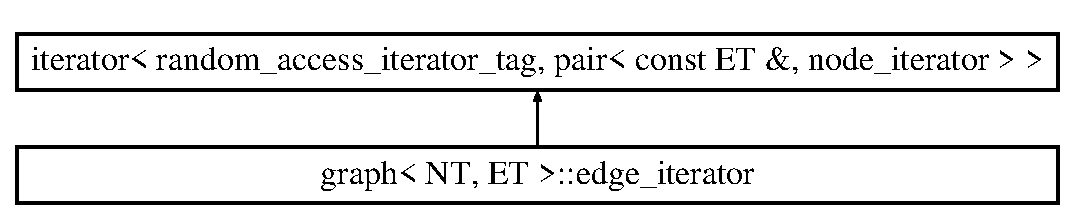
\includegraphics[height=2.000000cm]{classgraph_1_1edge__iterator}
\end{center}
\end{figure}
\subsection*{Public Member Functions}
\begin{DoxyCompactItemize}
\item 
\hyperlink{classgraph_1_1edge__iterator_a0718227c44321df4c54ac29cd55a7bb0}{edge\+\_\+iterator} ()
\begin{DoxyCompactList}\small\item\em Write what the function does here. \end{DoxyCompactList}\item 
\hypertarget{classgraph_1_1edge__iterator_a9f8774d21a021347e94238bde191464b}{{\bfseries edge\+\_\+iterator} (typename vector$<$ \hyperlink{structgraph_1_1Edge}{Edge} $\ast$ $>$\+::const\+\_\+iterator iter, const \hyperlink{classgraph}{graph} $\ast$g)}\label{classgraph_1_1edge__iterator_a9f8774d21a021347e94238bde191464b}

\item 
pair$<$ const E\+T \&, \hyperlink{classgraph_1_1node__iterator}{node\+\_\+iterator} $>$ \hyperlink{classgraph_1_1edge__iterator_ac36e53fb781544acaa92112ad71c59d5}{operator$\ast$} () const 
\begin{DoxyCompactList}\small\item\em Write what the function does here. \end{DoxyCompactList}\item 
const \hyperlink{classgraph_1_1edge__iterator}{edge\+\_\+iterator} \& \hyperlink{classgraph_1_1edge__iterator_ab8e3c8768c990af31d9fbb0de7e6e61f}{operator++} ()
\begin{DoxyCompactList}\small\item\em Write what the function does here. \end{DoxyCompactList}\item 
\hyperlink{classgraph_1_1edge__iterator}{edge\+\_\+iterator} \hyperlink{classgraph_1_1edge__iterator_a1b23686e252d3c458daa9ef212681d19}{operator++} (int)
\begin{DoxyCompactList}\small\item\em Write what the function does here. \end{DoxyCompactList}\item 
const \hyperlink{classgraph_1_1edge__iterator}{edge\+\_\+iterator} \& \hyperlink{classgraph_1_1edge__iterator_accb7545e2bc008e9a3e78c6b82a0274c}{operator-\/-\/} ()
\begin{DoxyCompactList}\small\item\em Write what the function does here. \end{DoxyCompactList}\item 
\hyperlink{classgraph_1_1edge__iterator}{edge\+\_\+iterator} \hyperlink{classgraph_1_1edge__iterator_af8d50792e43cd93274ddc5866fe941d7}{operator-\/-\/} (int)
\begin{DoxyCompactList}\small\item\em Write what the function does here. \end{DoxyCompactList}\item 
const \hyperlink{classgraph_1_1edge__iterator}{edge\+\_\+iterator} \& \hyperlink{classgraph_1_1edge__iterator_a5fab360b45d461a96a1d33d4537bd0fd}{operator+=} (int v)
\begin{DoxyCompactList}\small\item\em Write what the function does here. \end{DoxyCompactList}\item 
const \hyperlink{classgraph_1_1edge__iterator}{edge\+\_\+iterator} \& \hyperlink{classgraph_1_1edge__iterator_aaf9399c6beae614ea25f0601b61717ad}{operator-\/=} (int v)
\begin{DoxyCompactList}\small\item\em Write what the function does here. \end{DoxyCompactList}\item 
pair$<$ const E\+T \&, \hyperlink{classgraph_1_1node__iterator}{node\+\_\+iterator} $>$ \hyperlink{classgraph_1_1edge__iterator_aa37f36f86c3e59102bc4d79ab9b91a53}{operator\mbox{[}$\,$\mbox{]}} (int index) const 
\begin{DoxyCompactList}\small\item\em Write what the function does here. \end{DoxyCompactList}\item 
\hyperlink{classgraph_1_1node__iterator}{node\+\_\+iterator} \hyperlink{classgraph_1_1edge__iterator_a98a66e524bdfc1279aba7f8e04c18d33}{src} () const 
\begin{DoxyCompactList}\small\item\em Write what the function does here. \end{DoxyCompactList}\item 
\hyperlink{classgraph_1_1node__iterator}{node\+\_\+iterator} \hyperlink{classgraph_1_1edge__iterator_a2c9de7b09212f35c31308dee010c507d}{dest} () const 
\begin{DoxyCompactList}\small\item\em Write what the function does here. \end{DoxyCompactList}\end{DoxyCompactItemize}
\subsection*{Private Attributes}
\begin{DoxyCompactItemize}
\item 
\hypertarget{classgraph_1_1edge__iterator_a1a0a3fa0e4cd5ed6bb1304683a4ed3b0}{vector$<$ \hyperlink{structgraph_1_1Edge}{Edge} $\ast$ $>$\+::const\+\_\+iterator {\bfseries iter}}\label{classgraph_1_1edge__iterator_a1a0a3fa0e4cd5ed6bb1304683a4ed3b0}

\item 
\hypertarget{classgraph_1_1edge__iterator_a4232246807cc9b097f9c5196cc1e4ae5}{const \hyperlink{classgraph}{graph} $\ast$ {\bfseries g}}\label{classgraph_1_1edge__iterator_a4232246807cc9b097f9c5196cc1e4ae5}

\end{DoxyCompactItemize}
\subsection*{Friends}
\begin{DoxyCompactItemize}
\item 
bool \hyperlink{classgraph_1_1edge__iterator_a28e0f640c1891ad90508ba99546ec535}{operator==} (const \hyperlink{classgraph_1_1edge__iterator}{edge\+\_\+iterator} \&l, const \hyperlink{classgraph_1_1edge__iterator}{edge\+\_\+iterator} \&r)
\begin{DoxyCompactList}\small\item\em Write what the function does here. \end{DoxyCompactList}\item 
bool \hyperlink{classgraph_1_1edge__iterator_af3cf38a5594205c4367bbc054c85a507}{operator!=} (const \hyperlink{classgraph_1_1edge__iterator}{edge\+\_\+iterator} \&l, const \hyperlink{classgraph_1_1edge__iterator}{edge\+\_\+iterator} \&r)
\begin{DoxyCompactList}\small\item\em Write what the function does here. \end{DoxyCompactList}\item 
\hyperlink{classgraph_1_1edge__iterator}{edge\+\_\+iterator} \hyperlink{classgraph_1_1edge__iterator_a4ecd4e3679483eda13d5338fd4353d88}{operator+} (int v, const \hyperlink{classgraph_1_1edge__iterator}{edge\+\_\+iterator} \&iter)
\begin{DoxyCompactList}\small\item\em Write what the function does here. \end{DoxyCompactList}\item 
\hyperlink{classgraph_1_1edge__iterator}{edge\+\_\+iterator} \hyperlink{classgraph_1_1edge__iterator_a5dd36755f0bb84f84588c62aef5e5830}{operator+} (const \hyperlink{classgraph_1_1edge__iterator}{edge\+\_\+iterator} \&iter, int v)
\begin{DoxyCompactList}\small\item\em Write what the function does here. \end{DoxyCompactList}\item 
\hyperlink{classgraph_1_1edge__iterator}{edge\+\_\+iterator} \hyperlink{classgraph_1_1edge__iterator_a98fb2143e8ba5e7a043bd4c87c09814f}{operator-\/} (const \hyperlink{classgraph_1_1edge__iterator}{edge\+\_\+iterator} \&iter, int v)
\begin{DoxyCompactList}\small\item\em Write what the function does here. \end{DoxyCompactList}\item 
int \hyperlink{classgraph_1_1edge__iterator_a85016c8190c146f02194942120d797a2}{operator-\/} (const \hyperlink{classgraph_1_1edge__iterator}{edge\+\_\+iterator} \&l, const \hyperlink{classgraph_1_1edge__iterator}{edge\+\_\+iterator} \&r)
\begin{DoxyCompactList}\small\item\em Write what the function does here. \end{DoxyCompactList}\item 
bool \hyperlink{classgraph_1_1edge__iterator_a23a3dd85c962c0c5a4bf0b30e7696576}{operator$<$} (const \hyperlink{classgraph_1_1edge__iterator}{edge\+\_\+iterator} \&l, const \hyperlink{classgraph_1_1edge__iterator}{edge\+\_\+iterator} \&r)
\begin{DoxyCompactList}\small\item\em Write what the function does here. \end{DoxyCompactList}\item 
bool \hyperlink{classgraph_1_1edge__iterator_a301c07a77180ec86202103484fdfc7eb}{operator$<$=} (const \hyperlink{classgraph_1_1edge__iterator}{edge\+\_\+iterator} \&l, const \hyperlink{classgraph_1_1edge__iterator}{edge\+\_\+iterator} \&r)
\begin{DoxyCompactList}\small\item\em Write what the function does here. \end{DoxyCompactList}\item 
bool \hyperlink{classgraph_1_1edge__iterator_abd25c6fb3a8cc28addbb46e9775ce14c}{operator$>$=} (const \hyperlink{classgraph_1_1edge__iterator}{edge\+\_\+iterator} \&l, const \hyperlink{classgraph_1_1edge__iterator}{edge\+\_\+iterator} \&r)
\begin{DoxyCompactList}\small\item\em Write what the function does here. \end{DoxyCompactList}\item 
bool \hyperlink{classgraph_1_1edge__iterator_afb0a71f83c2fbd013fd42f6a91fdbc99}{operator$>$} (const \hyperlink{classgraph_1_1edge__iterator}{edge\+\_\+iterator} \&l, const \hyperlink{classgraph_1_1edge__iterator}{edge\+\_\+iterator} \&r)
\begin{DoxyCompactList}\small\item\em Write what the function does here. \end{DoxyCompactList}\end{DoxyCompactItemize}


\subsection{Detailed Description}
\subsubsection*{template$<$typename N\+T, typename E\+T = N\+T$>$class graph$<$ N\+T, E\+T $>$\+::edge\+\_\+iterator}



Definition at line 630 of file graph.\+h.



\subsection{Constructor \& Destructor Documentation}
\hypertarget{classgraph_1_1edge__iterator_a0718227c44321df4c54ac29cd55a7bb0}{\index{graph\+::edge\+\_\+iterator@{graph\+::edge\+\_\+iterator}!edge\+\_\+iterator@{edge\+\_\+iterator}}
\index{edge\+\_\+iterator@{edge\+\_\+iterator}!graph\+::edge\+\_\+iterator@{graph\+::edge\+\_\+iterator}}
\subsubsection[{edge\+\_\+iterator}]{\setlength{\rightskip}{0pt plus 5cm}template$<$typename N\+T , typename E\+T  = N\+T$>$ {\bf graph}$<$ N\+T, E\+T $>$\+::edge\+\_\+iterator\+::edge\+\_\+iterator (
\begin{DoxyParamCaption}
{}
\end{DoxyParamCaption}
)\hspace{0.3cm}{\ttfamily [inline]}}}\label{classgraph_1_1edge__iterator_a0718227c44321df4c54ac29cd55a7bb0}


Write what the function does here. 


\begin{DoxyRetVals}{Return values}
{\em (variable)} & (description of variable) \\
\hline
\end{DoxyRetVals}


Definition at line 651 of file graph.\+h.


\begin{DoxyCode}
652         \{
653         \}
\end{DoxyCode}


\subsection{Member Function Documentation}
\hypertarget{classgraph_1_1edge__iterator_a2c9de7b09212f35c31308dee010c507d}{\index{graph\+::edge\+\_\+iterator@{graph\+::edge\+\_\+iterator}!dest@{dest}}
\index{dest@{dest}!graph\+::edge\+\_\+iterator@{graph\+::edge\+\_\+iterator}}
\subsubsection[{dest}]{\setlength{\rightskip}{0pt plus 5cm}template$<$typename N\+T , typename E\+T  = N\+T$>$ {\bf node\+\_\+iterator} {\bf graph}$<$ N\+T, E\+T $>$\+::edge\+\_\+iterator\+::dest (
\begin{DoxyParamCaption}
{}
\end{DoxyParamCaption}
) const\hspace{0.3cm}{\ttfamily [inline]}}}\label{classgraph_1_1edge__iterator_a2c9de7b09212f35c31308dee010c507d}


Write what the function does here. 


\begin{DoxyRetVals}{Return values}
{\em (variable)} & (description of variable) \\
\hline
\end{DoxyRetVals}


Definition at line 898 of file graph.\+h.


\begin{DoxyCode}
899         \{
900             \textcolor{keywordflow}{return} node\_iterator((*iter)->dest->index, g);
901         \}
\end{DoxyCode}
\hypertarget{classgraph_1_1edge__iterator_ac36e53fb781544acaa92112ad71c59d5}{\index{graph\+::edge\+\_\+iterator@{graph\+::edge\+\_\+iterator}!operator$\ast$@{operator$\ast$}}
\index{operator$\ast$@{operator$\ast$}!graph\+::edge\+\_\+iterator@{graph\+::edge\+\_\+iterator}}
\subsubsection[{operator$\ast$}]{\setlength{\rightskip}{0pt plus 5cm}template$<$typename N\+T , typename E\+T  = N\+T$>$ pair$<$const E\+T \&, {\bf node\+\_\+iterator}$>$ {\bf graph}$<$ N\+T, E\+T $>$\+::edge\+\_\+iterator\+::operator$\ast$ (
\begin{DoxyParamCaption}
{}
\end{DoxyParamCaption}
) const\hspace{0.3cm}{\ttfamily [inline]}}}\label{classgraph_1_1edge__iterator_ac36e53fb781544acaa92112ad71c59d5}


Write what the function does here. 


\begin{DoxyRetVals}{Return values}
{\em (variable)} & (description of variable) \\
\hline
\end{DoxyRetVals}


Definition at line 690 of file graph.\+h.


\begin{DoxyCode}
691         \{
692             \textcolor{keywordflow}{return} pair<const ET &, node\_iterator>((*iter)->data, node\_iterator((*iter)->dest->index, g));
693         \}
\end{DoxyCode}
\hypertarget{classgraph_1_1edge__iterator_ab8e3c8768c990af31d9fbb0de7e6e61f}{\index{graph\+::edge\+\_\+iterator@{graph\+::edge\+\_\+iterator}!operator++@{operator++}}
\index{operator++@{operator++}!graph\+::edge\+\_\+iterator@{graph\+::edge\+\_\+iterator}}
\subsubsection[{operator++}]{\setlength{\rightskip}{0pt plus 5cm}template$<$typename N\+T , typename E\+T  = N\+T$>$ const {\bf edge\+\_\+iterator}\& {\bf graph}$<$ N\+T, E\+T $>$\+::edge\+\_\+iterator\+::operator++ (
\begin{DoxyParamCaption}
{}
\end{DoxyParamCaption}
)\hspace{0.3cm}{\ttfamily [inline]}}}\label{classgraph_1_1edge__iterator_ab8e3c8768c990af31d9fbb0de7e6e61f}


Write what the function does here. 


\begin{DoxyRetVals}{Return values}
{\em (variable)} & (description of variable) \\
\hline
\end{DoxyRetVals}


Definition at line 700 of file graph.\+h.


\begin{DoxyCode}
701         \{
702             ++iter;
703             \textcolor{keywordflow}{return} *\textcolor{keyword}{this};
704         \}
\end{DoxyCode}
\hypertarget{classgraph_1_1edge__iterator_a1b23686e252d3c458daa9ef212681d19}{\index{graph\+::edge\+\_\+iterator@{graph\+::edge\+\_\+iterator}!operator++@{operator++}}
\index{operator++@{operator++}!graph\+::edge\+\_\+iterator@{graph\+::edge\+\_\+iterator}}
\subsubsection[{operator++}]{\setlength{\rightskip}{0pt plus 5cm}template$<$typename N\+T , typename E\+T  = N\+T$>$ {\bf edge\+\_\+iterator} {\bf graph}$<$ N\+T, E\+T $>$\+::edge\+\_\+iterator\+::operator++ (
\begin{DoxyParamCaption}
\item[{int}]{}
\end{DoxyParamCaption}
)\hspace{0.3cm}{\ttfamily [inline]}}}\label{classgraph_1_1edge__iterator_a1b23686e252d3c458daa9ef212681d19}


Write what the function does here. 


\begin{DoxyParams}{Parameters}
{\em int} & \\
\hline
\end{DoxyParams}

\begin{DoxyRetVals}{Return values}
{\em (variable)} & (description of variable) \\
\hline
\end{DoxyRetVals}


Definition at line 713 of file graph.\+h.


\begin{DoxyCode}
714         \{
715             \textcolor{keywordflow}{return} \hyperlink{classgraph_1_1edge__iterator_a0718227c44321df4c54ac29cd55a7bb0}{edge\_iterator}(iter++, g);
716         \}
\end{DoxyCode}
\hypertarget{classgraph_1_1edge__iterator_a5fab360b45d461a96a1d33d4537bd0fd}{\index{graph\+::edge\+\_\+iterator@{graph\+::edge\+\_\+iterator}!operator+=@{operator+=}}
\index{operator+=@{operator+=}!graph\+::edge\+\_\+iterator@{graph\+::edge\+\_\+iterator}}
\subsubsection[{operator+=}]{\setlength{\rightskip}{0pt plus 5cm}template$<$typename N\+T , typename E\+T  = N\+T$>$ const {\bf edge\+\_\+iterator}\& {\bf graph}$<$ N\+T, E\+T $>$\+::edge\+\_\+iterator\+::operator+= (
\begin{DoxyParamCaption}
\item[{int}]{v}
\end{DoxyParamCaption}
)\hspace{0.3cm}{\ttfamily [inline]}}}\label{classgraph_1_1edge__iterator_a5fab360b45d461a96a1d33d4537bd0fd}


Write what the function does here. 


\begin{DoxyParams}{Parameters}
{\em v} & \\
\hline
\end{DoxyParams}

\begin{DoxyRetVals}{Return values}
{\em (variable)} & (description of variable) \\
\hline
\end{DoxyRetVals}


Definition at line 852 of file graph.\+h.


\begin{DoxyCode}
853         \{
854             iter += v;
855             \textcolor{keywordflow}{return} *\textcolor{keyword}{this};
856         \}
\end{DoxyCode}
\hypertarget{classgraph_1_1edge__iterator_accb7545e2bc008e9a3e78c6b82a0274c}{\index{graph\+::edge\+\_\+iterator@{graph\+::edge\+\_\+iterator}!operator-\/-\/@{operator-\/-\/}}
\index{operator-\/-\/@{operator-\/-\/}!graph\+::edge\+\_\+iterator@{graph\+::edge\+\_\+iterator}}
\subsubsection[{operator-\/-\/}]{\setlength{\rightskip}{0pt plus 5cm}template$<$typename N\+T , typename E\+T  = N\+T$>$ const {\bf edge\+\_\+iterator}\& {\bf graph}$<$ N\+T, E\+T $>$\+::edge\+\_\+iterator\+::operator-\/-\/ (
\begin{DoxyParamCaption}
{}
\end{DoxyParamCaption}
)\hspace{0.3cm}{\ttfamily [inline]}}}\label{classgraph_1_1edge__iterator_accb7545e2bc008e9a3e78c6b82a0274c}


Write what the function does here. 


\begin{DoxyRetVals}{Return values}
{\em (variable)} & (description of variable) \\
\hline
\end{DoxyRetVals}


Definition at line 723 of file graph.\+h.


\begin{DoxyCode}
724         \{
725             --iter;
726             \textcolor{keywordflow}{return} *\textcolor{keyword}{this};
727         \}
\end{DoxyCode}
\hypertarget{classgraph_1_1edge__iterator_af8d50792e43cd93274ddc5866fe941d7}{\index{graph\+::edge\+\_\+iterator@{graph\+::edge\+\_\+iterator}!operator-\/-\/@{operator-\/-\/}}
\index{operator-\/-\/@{operator-\/-\/}!graph\+::edge\+\_\+iterator@{graph\+::edge\+\_\+iterator}}
\subsubsection[{operator-\/-\/}]{\setlength{\rightskip}{0pt plus 5cm}template$<$typename N\+T , typename E\+T  = N\+T$>$ {\bf edge\+\_\+iterator} {\bf graph}$<$ N\+T, E\+T $>$\+::edge\+\_\+iterator\+::operator-\/-\/ (
\begin{DoxyParamCaption}
\item[{int}]{}
\end{DoxyParamCaption}
)\hspace{0.3cm}{\ttfamily [inline]}}}\label{classgraph_1_1edge__iterator_af8d50792e43cd93274ddc5866fe941d7}


Write what the function does here. 


\begin{DoxyParams}{Parameters}
{\em int} & \\
\hline
\end{DoxyParams}

\begin{DoxyRetVals}{Return values}
{\em (variable)} & (description of variable) \\
\hline
\end{DoxyRetVals}


Definition at line 736 of file graph.\+h.


\begin{DoxyCode}
737         \{
738             \textcolor{keywordflow}{return} \hyperlink{classgraph_1_1edge__iterator_a0718227c44321df4c54ac29cd55a7bb0}{edge\_iterator}(iter--, g);
739         \}
\end{DoxyCode}
\hypertarget{classgraph_1_1edge__iterator_aaf9399c6beae614ea25f0601b61717ad}{\index{graph\+::edge\+\_\+iterator@{graph\+::edge\+\_\+iterator}!operator-\/=@{operator-\/=}}
\index{operator-\/=@{operator-\/=}!graph\+::edge\+\_\+iterator@{graph\+::edge\+\_\+iterator}}
\subsubsection[{operator-\/=}]{\setlength{\rightskip}{0pt plus 5cm}template$<$typename N\+T , typename E\+T  = N\+T$>$ const {\bf edge\+\_\+iterator}\& {\bf graph}$<$ N\+T, E\+T $>$\+::edge\+\_\+iterator\+::operator-\/= (
\begin{DoxyParamCaption}
\item[{int}]{v}
\end{DoxyParamCaption}
)\hspace{0.3cm}{\ttfamily [inline]}}}\label{classgraph_1_1edge__iterator_aaf9399c6beae614ea25f0601b61717ad}


Write what the function does here. 


\begin{DoxyParams}{Parameters}
{\em v} & \\
\hline
\end{DoxyParams}

\begin{DoxyRetVals}{Return values}
{\em (variable)} & (description of variable) \\
\hline
\end{DoxyRetVals}


Definition at line 865 of file graph.\+h.


\begin{DoxyCode}
866         \{
867             iter -= v;
868             \textcolor{keywordflow}{return} *\textcolor{keyword}{this};
869         \}
\end{DoxyCode}
\hypertarget{classgraph_1_1edge__iterator_aa37f36f86c3e59102bc4d79ab9b91a53}{\index{graph\+::edge\+\_\+iterator@{graph\+::edge\+\_\+iterator}!operator\mbox{[}$\,$\mbox{]}@{operator[]}}
\index{operator\mbox{[}$\,$\mbox{]}@{operator[]}!graph\+::edge\+\_\+iterator@{graph\+::edge\+\_\+iterator}}
\subsubsection[{operator[]}]{\setlength{\rightskip}{0pt plus 5cm}template$<$typename N\+T , typename E\+T  = N\+T$>$ pair$<$const E\+T \&, {\bf node\+\_\+iterator}$>$ {\bf graph}$<$ N\+T, E\+T $>$\+::edge\+\_\+iterator\+::operator\mbox{[}$\,$\mbox{]} (
\begin{DoxyParamCaption}
\item[{int}]{index}
\end{DoxyParamCaption}
) const\hspace{0.3cm}{\ttfamily [inline]}}}\label{classgraph_1_1edge__iterator_aa37f36f86c3e59102bc4d79ab9b91a53}


Write what the function does here. 


\begin{DoxyParams}{Parameters}
{\em index} & \\
\hline
\end{DoxyParams}

\begin{DoxyRetVals}{Return values}
{\em (variable)} & (description of variable) \\
\hline
\end{DoxyRetVals}


Definition at line 878 of file graph.\+h.


\begin{DoxyCode}
879         \{
880             \textcolor{keywordflow}{return} *(*\textcolor{keyword}{this} + index);
881         \}
\end{DoxyCode}
\hypertarget{classgraph_1_1edge__iterator_a98a66e524bdfc1279aba7f8e04c18d33}{\index{graph\+::edge\+\_\+iterator@{graph\+::edge\+\_\+iterator}!src@{src}}
\index{src@{src}!graph\+::edge\+\_\+iterator@{graph\+::edge\+\_\+iterator}}
\subsubsection[{src}]{\setlength{\rightskip}{0pt plus 5cm}template$<$typename N\+T , typename E\+T  = N\+T$>$ {\bf node\+\_\+iterator} {\bf graph}$<$ N\+T, E\+T $>$\+::edge\+\_\+iterator\+::src (
\begin{DoxyParamCaption}
{}
\end{DoxyParamCaption}
) const\hspace{0.3cm}{\ttfamily [inline]}}}\label{classgraph_1_1edge__iterator_a98a66e524bdfc1279aba7f8e04c18d33}


Write what the function does here. 


\begin{DoxyRetVals}{Return values}
{\em (variable)} & (description of variable) \\
\hline
\end{DoxyRetVals}


Definition at line 888 of file graph.\+h.


\begin{DoxyCode}
889         \{
890             \textcolor{keywordflow}{return} node\_iterator((*iter)->src->index, g);
891         \}
\end{DoxyCode}


\subsection{Friends And Related Function Documentation}
\hypertarget{classgraph_1_1edge__iterator_af3cf38a5594205c4367bbc054c85a507}{\index{graph\+::edge\+\_\+iterator@{graph\+::edge\+\_\+iterator}!operator"!=@{operator"!=}}
\index{operator"!=@{operator"!=}!graph\+::edge\+\_\+iterator@{graph\+::edge\+\_\+iterator}}
\subsubsection[{operator"!=}]{\setlength{\rightskip}{0pt plus 5cm}template$<$typename N\+T , typename E\+T  = N\+T$>$ bool operator!= (
\begin{DoxyParamCaption}
\item[{const {\bf edge\+\_\+iterator} \&}]{l, }
\item[{const {\bf edge\+\_\+iterator} \&}]{r}
\end{DoxyParamCaption}
)\hspace{0.3cm}{\ttfamily [friend]}}}\label{classgraph_1_1edge__iterator_af3cf38a5594205c4367bbc054c85a507}


Write what the function does here. 


\begin{DoxyParams}{Parameters}
{\em l} & \\
\hline
{\em r} & \\
\hline
\end{DoxyParams}

\begin{DoxyRetVals}{Return values}
{\em (variable)} & (description of variable) \\
\hline
\end{DoxyRetVals}


Definition at line 680 of file graph.\+h.


\begin{DoxyCode}
681         \{
682             \textcolor{keywordflow}{return} l.iter != r.iter;
683         \}
\end{DoxyCode}
\hypertarget{classgraph_1_1edge__iterator_a4ecd4e3679483eda13d5338fd4353d88}{\index{graph\+::edge\+\_\+iterator@{graph\+::edge\+\_\+iterator}!operator+@{operator+}}
\index{operator+@{operator+}!graph\+::edge\+\_\+iterator@{graph\+::edge\+\_\+iterator}}
\subsubsection[{operator+}]{\setlength{\rightskip}{0pt plus 5cm}template$<$typename N\+T , typename E\+T  = N\+T$>$ {\bf edge\+\_\+iterator} operator+ (
\begin{DoxyParamCaption}
\item[{int}]{v, }
\item[{const {\bf edge\+\_\+iterator} \&}]{iter}
\end{DoxyParamCaption}
)\hspace{0.3cm}{\ttfamily [friend]}}}\label{classgraph_1_1edge__iterator_a4ecd4e3679483eda13d5338fd4353d88}


Write what the function does here. 


\begin{DoxyParams}{Parameters}
{\em v} & \\
\hline
{\em iter} & \\
\hline
\end{DoxyParams}

\begin{DoxyRetVals}{Return values}
{\em (variable)} & (description of variable) \\
\hline
\end{DoxyRetVals}


Definition at line 749 of file graph.\+h.


\begin{DoxyCode}
750         \{
751             \textcolor{keywordflow}{return} \hyperlink{classgraph_1_1edge__iterator_a0718227c44321df4c54ac29cd55a7bb0}{edge\_iterator}(v + iter.iter, iter.g);
752         \}
\end{DoxyCode}
\hypertarget{classgraph_1_1edge__iterator_a5dd36755f0bb84f84588c62aef5e5830}{\index{graph\+::edge\+\_\+iterator@{graph\+::edge\+\_\+iterator}!operator+@{operator+}}
\index{operator+@{operator+}!graph\+::edge\+\_\+iterator@{graph\+::edge\+\_\+iterator}}
\subsubsection[{operator+}]{\setlength{\rightskip}{0pt plus 5cm}template$<$typename N\+T , typename E\+T  = N\+T$>$ {\bf edge\+\_\+iterator} operator+ (
\begin{DoxyParamCaption}
\item[{const {\bf edge\+\_\+iterator} \&}]{iter, }
\item[{int}]{v}
\end{DoxyParamCaption}
)\hspace{0.3cm}{\ttfamily [friend]}}}\label{classgraph_1_1edge__iterator_a5dd36755f0bb84f84588c62aef5e5830}


Write what the function does here. 


\begin{DoxyParams}{Parameters}
{\em iter} & \\
\hline
{\em v} & \\
\hline
\end{DoxyParams}

\begin{DoxyRetVals}{Return values}
{\em (variable)} & (description of variable) \\
\hline
\end{DoxyRetVals}


Definition at line 762 of file graph.\+h.


\begin{DoxyCode}
763         \{
764             \textcolor{keywordflow}{return} \hyperlink{classgraph_1_1edge__iterator_a0718227c44321df4c54ac29cd55a7bb0}{edge\_iterator}(iter.iter + v, iter.g);
765         \}
\end{DoxyCode}
\hypertarget{classgraph_1_1edge__iterator_a98fb2143e8ba5e7a043bd4c87c09814f}{\index{graph\+::edge\+\_\+iterator@{graph\+::edge\+\_\+iterator}!operator-\/@{operator-\/}}
\index{operator-\/@{operator-\/}!graph\+::edge\+\_\+iterator@{graph\+::edge\+\_\+iterator}}
\subsubsection[{operator-\/}]{\setlength{\rightskip}{0pt plus 5cm}template$<$typename N\+T , typename E\+T  = N\+T$>$ {\bf edge\+\_\+iterator} operator-\/ (
\begin{DoxyParamCaption}
\item[{const {\bf edge\+\_\+iterator} \&}]{iter, }
\item[{int}]{v}
\end{DoxyParamCaption}
)\hspace{0.3cm}{\ttfamily [friend]}}}\label{classgraph_1_1edge__iterator_a98fb2143e8ba5e7a043bd4c87c09814f}


Write what the function does here. 


\begin{DoxyParams}{Parameters}
{\em iter} & \\
\hline
{\em v} & \\
\hline
\end{DoxyParams}

\begin{DoxyRetVals}{Return values}
{\em (variable)} & (description of variable) \\
\hline
\end{DoxyRetVals}


Definition at line 775 of file graph.\+h.


\begin{DoxyCode}
776         \{
777             \textcolor{keywordflow}{return} \hyperlink{classgraph_1_1edge__iterator_a0718227c44321df4c54ac29cd55a7bb0}{edge\_iterator}(iter.iter - v, iter.g);
778         \}
\end{DoxyCode}
\hypertarget{classgraph_1_1edge__iterator_a85016c8190c146f02194942120d797a2}{\index{graph\+::edge\+\_\+iterator@{graph\+::edge\+\_\+iterator}!operator-\/@{operator-\/}}
\index{operator-\/@{operator-\/}!graph\+::edge\+\_\+iterator@{graph\+::edge\+\_\+iterator}}
\subsubsection[{operator-\/}]{\setlength{\rightskip}{0pt plus 5cm}template$<$typename N\+T , typename E\+T  = N\+T$>$ int operator-\/ (
\begin{DoxyParamCaption}
\item[{const {\bf edge\+\_\+iterator} \&}]{l, }
\item[{const {\bf edge\+\_\+iterator} \&}]{r}
\end{DoxyParamCaption}
)\hspace{0.3cm}{\ttfamily [friend]}}}\label{classgraph_1_1edge__iterator_a85016c8190c146f02194942120d797a2}


Write what the function does here. 


\begin{DoxyParams}{Parameters}
{\em l} & \\
\hline
{\em r} & \\
\hline
\end{DoxyParams}

\begin{DoxyRetVals}{Return values}
{\em (variable)} & (description of variable) \\
\hline
\end{DoxyRetVals}


Definition at line 788 of file graph.\+h.


\begin{DoxyCode}
789         \{
790             \textcolor{keywordflow}{return} l.iter - r.iter;
791         \}
\end{DoxyCode}
\hypertarget{classgraph_1_1edge__iterator_a23a3dd85c962c0c5a4bf0b30e7696576}{\index{graph\+::edge\+\_\+iterator@{graph\+::edge\+\_\+iterator}!operator$<$@{operator$<$}}
\index{operator$<$@{operator$<$}!graph\+::edge\+\_\+iterator@{graph\+::edge\+\_\+iterator}}
\subsubsection[{operator$<$}]{\setlength{\rightskip}{0pt plus 5cm}template$<$typename N\+T , typename E\+T  = N\+T$>$ bool operator$<$ (
\begin{DoxyParamCaption}
\item[{const {\bf edge\+\_\+iterator} \&}]{l, }
\item[{const {\bf edge\+\_\+iterator} \&}]{r}
\end{DoxyParamCaption}
)\hspace{0.3cm}{\ttfamily [friend]}}}\label{classgraph_1_1edge__iterator_a23a3dd85c962c0c5a4bf0b30e7696576}


Write what the function does here. 


\begin{DoxyParams}{Parameters}
{\em l} & \\
\hline
{\em r} & \\
\hline
\end{DoxyParams}

\begin{DoxyRetVals}{Return values}
{\em (variable)} & (description of variable) \\
\hline
\end{DoxyRetVals}


Definition at line 801 of file graph.\+h.


\begin{DoxyCode}
802         \{
803             \textcolor{keywordflow}{return} l.iter < r.iter;
804         \}
\end{DoxyCode}
\hypertarget{classgraph_1_1edge__iterator_a301c07a77180ec86202103484fdfc7eb}{\index{graph\+::edge\+\_\+iterator@{graph\+::edge\+\_\+iterator}!operator$<$=@{operator$<$=}}
\index{operator$<$=@{operator$<$=}!graph\+::edge\+\_\+iterator@{graph\+::edge\+\_\+iterator}}
\subsubsection[{operator$<$=}]{\setlength{\rightskip}{0pt plus 5cm}template$<$typename N\+T , typename E\+T  = N\+T$>$ bool operator$<$= (
\begin{DoxyParamCaption}
\item[{const {\bf edge\+\_\+iterator} \&}]{l, }
\item[{const {\bf edge\+\_\+iterator} \&}]{r}
\end{DoxyParamCaption}
)\hspace{0.3cm}{\ttfamily [friend]}}}\label{classgraph_1_1edge__iterator_a301c07a77180ec86202103484fdfc7eb}


Write what the function does here. 


\begin{DoxyParams}{Parameters}
{\em l} & \\
\hline
{\em r} & \\
\hline
\end{DoxyParams}

\begin{DoxyRetVals}{Return values}
{\em (variable)} & (description of variable) \\
\hline
\end{DoxyRetVals}


Definition at line 814 of file graph.\+h.


\begin{DoxyCode}
815         \{
816             \textcolor{keywordflow}{return} l.iter <= r.iter;
817         \}
\end{DoxyCode}
\hypertarget{classgraph_1_1edge__iterator_a28e0f640c1891ad90508ba99546ec535}{\index{graph\+::edge\+\_\+iterator@{graph\+::edge\+\_\+iterator}!operator==@{operator==}}
\index{operator==@{operator==}!graph\+::edge\+\_\+iterator@{graph\+::edge\+\_\+iterator}}
\subsubsection[{operator==}]{\setlength{\rightskip}{0pt plus 5cm}template$<$typename N\+T , typename E\+T  = N\+T$>$ bool operator== (
\begin{DoxyParamCaption}
\item[{const {\bf edge\+\_\+iterator} \&}]{l, }
\item[{const {\bf edge\+\_\+iterator} \&}]{r}
\end{DoxyParamCaption}
)\hspace{0.3cm}{\ttfamily [friend]}}}\label{classgraph_1_1edge__iterator_a28e0f640c1891ad90508ba99546ec535}


Write what the function does here. 


\begin{DoxyParams}{Parameters}
{\em l} & \\
\hline
{\em r} & \\
\hline
\end{DoxyParams}

\begin{DoxyRetVals}{Return values}
{\em (variable)} & (description of variable) \\
\hline
\end{DoxyRetVals}


Definition at line 667 of file graph.\+h.


\begin{DoxyCode}
668         \{
669             \textcolor{keywordflow}{return} l.iter == r.iter;
670         \}
\end{DoxyCode}
\hypertarget{classgraph_1_1edge__iterator_afb0a71f83c2fbd013fd42f6a91fdbc99}{\index{graph\+::edge\+\_\+iterator@{graph\+::edge\+\_\+iterator}!operator$>$@{operator$>$}}
\index{operator$>$@{operator$>$}!graph\+::edge\+\_\+iterator@{graph\+::edge\+\_\+iterator}}
\subsubsection[{operator$>$}]{\setlength{\rightskip}{0pt plus 5cm}template$<$typename N\+T , typename E\+T  = N\+T$>$ bool operator$>$ (
\begin{DoxyParamCaption}
\item[{const {\bf edge\+\_\+iterator} \&}]{l, }
\item[{const {\bf edge\+\_\+iterator} \&}]{r}
\end{DoxyParamCaption}
)\hspace{0.3cm}{\ttfamily [friend]}}}\label{classgraph_1_1edge__iterator_afb0a71f83c2fbd013fd42f6a91fdbc99}


Write what the function does here. 


\begin{DoxyParams}{Parameters}
{\em l} & \\
\hline
{\em r} & \\
\hline
\end{DoxyParams}

\begin{DoxyRetVals}{Return values}
{\em (variable)} & (description of variable) \\
\hline
\end{DoxyRetVals}


Definition at line 840 of file graph.\+h.


\begin{DoxyCode}
841         \{
842             \textcolor{keywordflow}{return} l.iter > r.iter;
843         \}
\end{DoxyCode}
\hypertarget{classgraph_1_1edge__iterator_abd25c6fb3a8cc28addbb46e9775ce14c}{\index{graph\+::edge\+\_\+iterator@{graph\+::edge\+\_\+iterator}!operator$>$=@{operator$>$=}}
\index{operator$>$=@{operator$>$=}!graph\+::edge\+\_\+iterator@{graph\+::edge\+\_\+iterator}}
\subsubsection[{operator$>$=}]{\setlength{\rightskip}{0pt plus 5cm}template$<$typename N\+T , typename E\+T  = N\+T$>$ bool operator$>$= (
\begin{DoxyParamCaption}
\item[{const {\bf edge\+\_\+iterator} \&}]{l, }
\item[{const {\bf edge\+\_\+iterator} \&}]{r}
\end{DoxyParamCaption}
)\hspace{0.3cm}{\ttfamily [friend]}}}\label{classgraph_1_1edge__iterator_abd25c6fb3a8cc28addbb46e9775ce14c}


Write what the function does here. 


\begin{DoxyParams}{Parameters}
{\em l} & \\
\hline
{\em r} & \\
\hline
\end{DoxyParams}

\begin{DoxyRetVals}{Return values}
{\em (variable)} & (description of variable) \\
\hline
\end{DoxyRetVals}


Definition at line 827 of file graph.\+h.


\begin{DoxyCode}
828         \{
829             \textcolor{keywordflow}{return} l.iter >= r.iter;
830         \}
\end{DoxyCode}


The documentation for this class was generated from the following file\+:\begin{DoxyCompactItemize}
\item 
graph.\+h\end{DoxyCompactItemize}

\hypertarget{classEOFException}{\section{E\+O\+F\+Exception Class Reference}
\label{classEOFException}\index{E\+O\+F\+Exception@{E\+O\+F\+Exception}}
}


Write what the function does here.  




{\ttfamily \#include $<$stream.\+h$>$}

Inheritance diagram for E\+O\+F\+Exception\+:\begin{figure}[H]
\begin{center}
\leavevmode
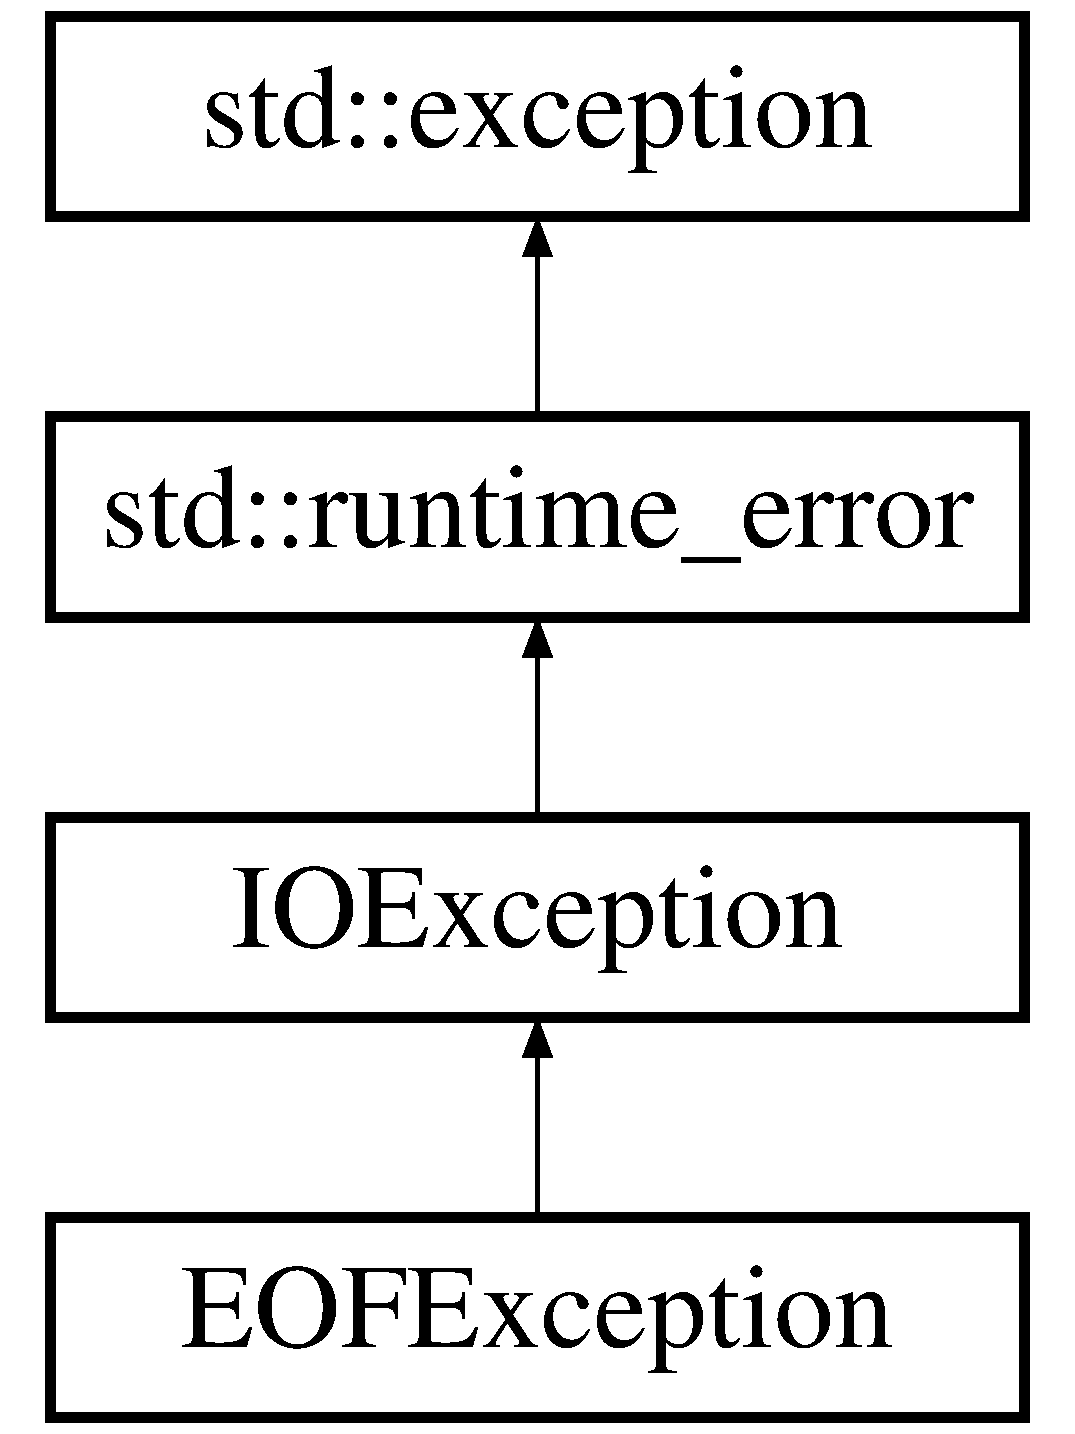
\includegraphics[height=4.000000cm]{classEOFException}
\end{center}
\end{figure}
\subsection*{Additional Inherited Members}


\subsection{Detailed Description}
Write what the function does here. 

\begin{DoxyReturn}{Returns}

\end{DoxyReturn}


Definition at line 56 of file stream.\+h.



The documentation for this class was generated from the following file\+:\begin{DoxyCompactItemize}
\item 
stream.\+h\end{DoxyCompactItemize}

\hypertarget{classEvent}{\section{Event Class Reference}
\label{classEvent}\index{Event@{Event}}
}


Write what the function does here.  




{\ttfamily \#include $<$event.\+h$>$}

Inheritance diagram for Event\+:\begin{figure}[H]
\begin{center}
\leavevmode
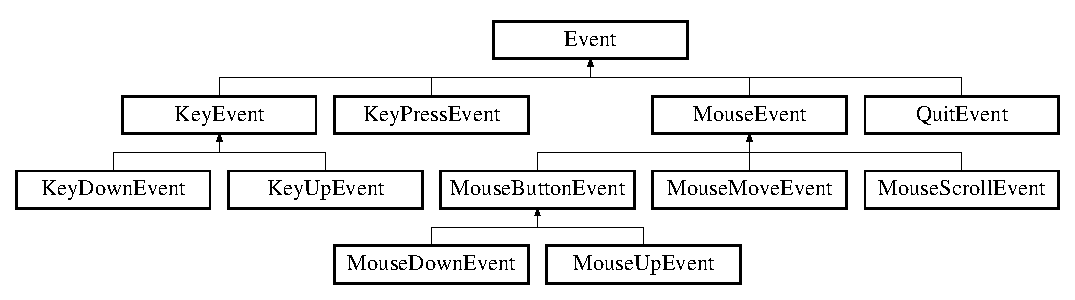
\includegraphics[height=3.584000cm]{classEvent}
\end{center}
\end{figure}
\subsection*{Public Types}
\begin{DoxyCompactItemize}
\item 
enum \hyperlink{classEvent_a2abf13b5be49315e9e362af02029f058}{Type} \{ \\*
{\bfseries Type\+\_\+\+Mouse\+Up}, 
{\bfseries Type\+\_\+\+Mouse\+Down}, 
{\bfseries Type\+\_\+\+Mouse\+Move}, 
{\bfseries Type\+\_\+\+Mouse\+Scroll}, 
\\*
{\bfseries Type\+\_\+\+Key\+Up}, 
{\bfseries Type\+\_\+\+Key\+Down}, 
{\bfseries Type\+\_\+\+Key\+Press}, 
{\bfseries Type\+\_\+\+Quit}
 \}
\begin{DoxyCompactList}\small\item\em Write what the function does here. \end{DoxyCompactList}\end{DoxyCompactItemize}
\subsection*{Public Member Functions}
\begin{DoxyCompactItemize}
\item 
\hypertarget{classEvent_a505136f7f21d062f315cf4827c939068}{virtual bool {\bfseries dispatch} (shared\+\_\+ptr$<$ \hyperlink{structEventHandler}{Event\+Handler} $>$ event\+Handler)=0}\label{classEvent_a505136f7f21d062f315cf4827c939068}

\end{DoxyCompactItemize}
\subsection*{Public Attributes}
\begin{DoxyCompactItemize}
\item 
\hypertarget{classEvent_a86404000a5e0b6b3afdb2c88d4923e3b}{const \hyperlink{classEvent_a2abf13b5be49315e9e362af02029f058}{Type} {\bfseries type}}\label{classEvent_a86404000a5e0b6b3afdb2c88d4923e3b}

\end{DoxyCompactItemize}
\subsection*{Protected Member Functions}
\begin{DoxyCompactItemize}
\item 
\hypertarget{classEvent_a07dd964621d0623bfccc24197c2f509b}{{\bfseries Event} (\hyperlink{classEvent_a2abf13b5be49315e9e362af02029f058}{Type} type)}\label{classEvent_a07dd964621d0623bfccc24197c2f509b}

\end{DoxyCompactItemize}


\subsection{Detailed Description}
Write what the function does here. 

\begin{DoxyReturn}{Returns}

\end{DoxyReturn}


Definition at line 37 of file event.\+h.



\subsection{Member Enumeration Documentation}
\hypertarget{classEvent_a2abf13b5be49315e9e362af02029f058}{\index{Event@{Event}!Type@{Type}}
\index{Type@{Type}!Event@{Event}}
\subsubsection[{Type}]{\setlength{\rightskip}{0pt plus 5cm}enum {\bf Event\+::\+Type}}}\label{classEvent_a2abf13b5be49315e9e362af02029f058}


Write what the function does here. 

\begin{DoxyReturn}{Returns}

\end{DoxyReturn}


Definition at line 46 of file event.\+h.


\begin{DoxyCode}
47         \{
48             Type\_MouseUp,
49             Type\_MouseDown,
50             Type\_MouseMove,
51             Type\_MouseScroll,
52             Type\_KeyUp,
53             Type\_KeyDown,
54             Type\_KeyPress,
55             Type\_Quit,
56         \};
\end{DoxyCode}


The documentation for this class was generated from the following file\+:\begin{DoxyCompactItemize}
\item 
event.\+h\end{DoxyCompactItemize}

\hypertarget{structEventHandler}{\section{Event\+Handler Struct Reference}
\label{structEventHandler}\index{Event\+Handler@{Event\+Handler}}
}


Write what the function does here.  




{\ttfamily \#include $<$event.\+h$>$}

Inheritance diagram for Event\+Handler\+:\begin{figure}[H]
\begin{center}
\leavevmode
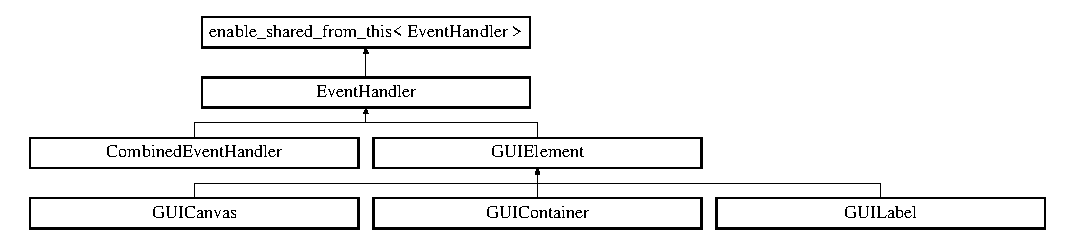
\includegraphics[height=2.839037cm]{structEventHandler}
\end{center}
\end{figure}
\subsection*{Public Member Functions}
\begin{DoxyCompactItemize}
\item 
\hypertarget{structEventHandler_a31b9dcd55c5bddebb875765576255e90}{virtual bool {\bfseries handle\+Mouse\+Up} (\hyperlink{structMouseUpEvent}{Mouse\+Up\+Event} \&\hyperlink{unionSDL__Event}{event})=0}\label{structEventHandler_a31b9dcd55c5bddebb875765576255e90}

\item 
\hypertarget{structEventHandler_a4a3f362f4dbc700af1fad213131c7e0e}{virtual bool {\bfseries handle\+Mouse\+Down} (\hyperlink{structMouseDownEvent}{Mouse\+Down\+Event} \&\hyperlink{unionSDL__Event}{event})=0}\label{structEventHandler_a4a3f362f4dbc700af1fad213131c7e0e}

\item 
\hypertarget{structEventHandler_a62e75bc38f855bc1d7f677225f601345}{virtual bool {\bfseries handle\+Mouse\+Move} (\hyperlink{structMouseMoveEvent}{Mouse\+Move\+Event} \&\hyperlink{unionSDL__Event}{event})=0}\label{structEventHandler_a62e75bc38f855bc1d7f677225f601345}

\item 
\hypertarget{structEventHandler_a7fa1d4c71f4f97a12c1203676bb50f9f}{virtual bool {\bfseries handle\+Mouse\+Scroll} (\hyperlink{structMouseScrollEvent}{Mouse\+Scroll\+Event} \&\hyperlink{unionSDL__Event}{event})=0}\label{structEventHandler_a7fa1d4c71f4f97a12c1203676bb50f9f}

\item 
\hypertarget{structEventHandler_af209b5af92d670e20a3c4b6acf8c32e3}{virtual bool {\bfseries handle\+Key\+Up} (\hyperlink{classKeyUpEvent}{Key\+Up\+Event} \&\hyperlink{unionSDL__Event}{event})=0}\label{structEventHandler_af209b5af92d670e20a3c4b6acf8c32e3}

\item 
\hypertarget{structEventHandler_affc191abd86c8cdd3290a4b9229a4c2f}{virtual bool {\bfseries handle\+Key\+Down} (\hyperlink{classKeyDownEvent}{Key\+Down\+Event} \&\hyperlink{unionSDL__Event}{event})=0}\label{structEventHandler_affc191abd86c8cdd3290a4b9229a4c2f}

\item 
\hypertarget{structEventHandler_a2db8a056203bd5a6c2f2d7045dd0dcf9}{virtual bool {\bfseries handle\+Key\+Press} (\hyperlink{structKeyPressEvent}{Key\+Press\+Event} \&\hyperlink{unionSDL__Event}{event})=0}\label{structEventHandler_a2db8a056203bd5a6c2f2d7045dd0dcf9}

\item 
\hypertarget{structEventHandler_a7edb38ef218c53ccfe5a9e17a78e865d}{virtual bool {\bfseries handle\+Quit} (\hyperlink{structQuitEvent}{Quit\+Event} \&\hyperlink{unionSDL__Event}{event})=0}\label{structEventHandler_a7edb38ef218c53ccfe5a9e17a78e865d}

\end{DoxyCompactItemize}


\subsection{Detailed Description}
Write what the function does here. 


\begin{DoxyRetVals}{Return values}
{\em (variable)} & (description of variable) \\
\hline
\end{DoxyRetVals}


Definition at line 20 of file event.\+h.



The documentation for this struct was generated from the following file\+:\begin{DoxyCompactItemize}
\item 
event.\+h\end{DoxyCompactItemize}

\hypertarget{classExpandReader}{\section{Expand\+Reader Class Reference}
\label{classExpandReader}\index{Expand\+Reader@{Expand\+Reader}}
}


Write what the function does here.  




{\ttfamily \#include $<$compressed\+\_\+stream.\+h$>$}

Inheritance diagram for Expand\+Reader\+:\begin{figure}[H]
\begin{center}
\leavevmode
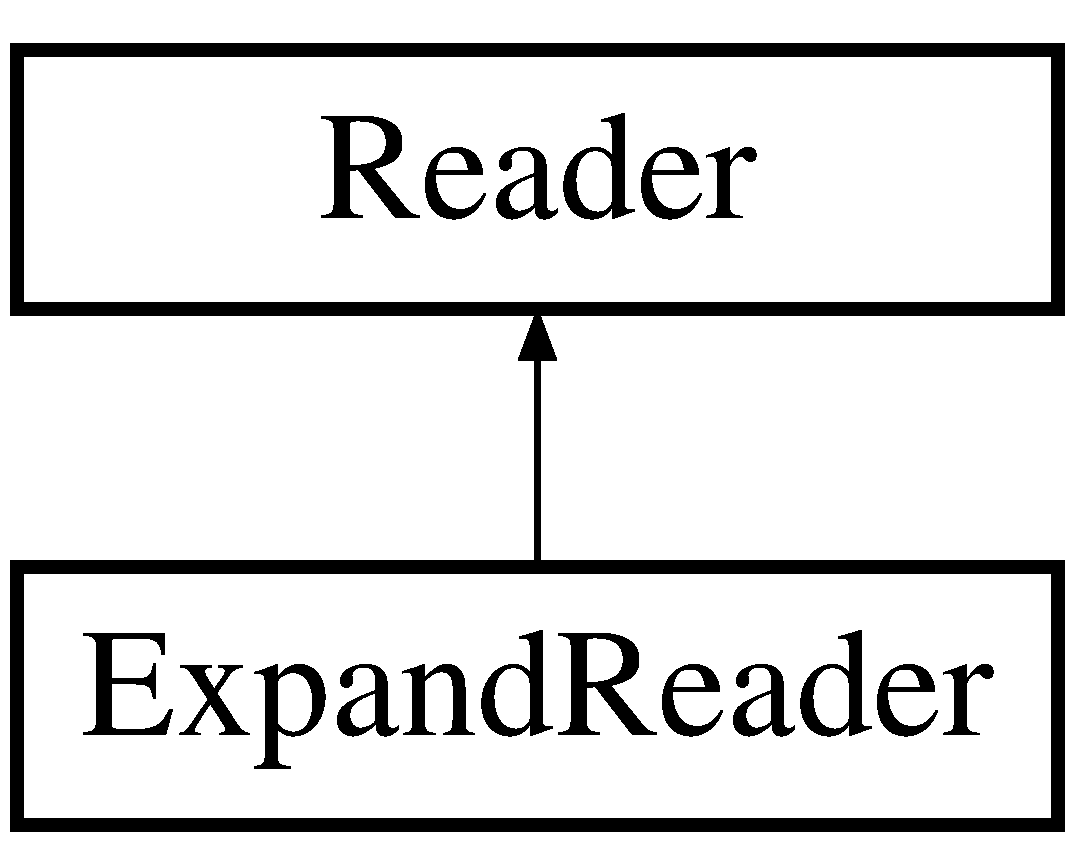
\includegraphics[height=2.000000cm]{classExpandReader}
\end{center}
\end{figure}
\subsection*{Public Member Functions}
\begin{DoxyCompactItemize}
\item 
\hypertarget{classExpandReader_a6e08c2a0ddfcaf4039364a7d5b86c713}{{\bfseries Expand\+Reader} (shared\+\_\+ptr$<$ \hyperlink{classReader}{Reader} $>$ reader)}\label{classExpandReader_a6e08c2a0ddfcaf4039364a7d5b86c713}

\item 
\hyperlink{classExpandReader_acff92ec084cb738b0a072fcad2096e45}{Expand\+Reader} (\hyperlink{classReader}{Reader} \&reader)
\begin{DoxyCompactList}\small\item\em Write what the function does here. \end{DoxyCompactList}\item 
\hypertarget{classExpandReader_ad3339a664afce44dbba5ceb3cf9b6ebd}{virtual uint8\+\_\+t {\bfseries read\+Byte} () override}\label{classExpandReader_ad3339a664afce44dbba5ceb3cf9b6ebd}

\end{DoxyCompactItemize}
\subsection*{Private Attributes}
\begin{DoxyCompactItemize}
\item 
\hypertarget{classExpandReader_abb317fa1dae74a6f01efb916dc1f1a78}{shared\+\_\+ptr$<$ \hyperlink{classReader}{Reader} $>$ {\bfseries reader}}\label{classExpandReader_abb317fa1dae74a6f01efb916dc1f1a78}

\item 
\hypertarget{classExpandReader_a75ba7c441e5d85a84432604ddbdaa734}{\hyperlink{classcircularDeque}{circular\+Deque}$<$ uint8\+\_\+t, \\*
buffer\+Size+2 $>$ {\bfseries buffer}}\label{classExpandReader_a75ba7c441e5d85a84432604ddbdaa734}

\item 
\hypertarget{classExpandReader_a3829efc17d18ef7a90c05177cea0a402}{\hyperlink{structLZ77CodeType}{L\+Z77\+Code\+Type} {\bfseries current\+Code}}\label{classExpandReader_a3829efc17d18ef7a90c05177cea0a402}

\end{DoxyCompactItemize}
\subsection*{Static Private Attributes}
\begin{DoxyCompactItemize}
\item 
\hypertarget{classExpandReader_aea9fc5ac4ca868bf23dbe48022f81d53}{static constexpr size\+\_\+t {\bfseries buffer\+Size} = L\+Z77\+Code\+Type\+::max\+Offset + 1}\label{classExpandReader_aea9fc5ac4ca868bf23dbe48022f81d53}

\end{DoxyCompactItemize}


\subsection{Detailed Description}
Write what the function does here. 


\begin{DoxyRetVals}{Return values}
{\em (variable)} & (description of variable) \\
\hline
\end{DoxyRetVals}


Definition at line 111 of file compressed\+\_\+stream.\+h.



\subsection{Constructor \& Destructor Documentation}
\hypertarget{classExpandReader_acff92ec084cb738b0a072fcad2096e45}{\index{Expand\+Reader@{Expand\+Reader}!Expand\+Reader@{Expand\+Reader}}
\index{Expand\+Reader@{Expand\+Reader}!Expand\+Reader@{Expand\+Reader}}
\subsubsection[{Expand\+Reader}]{\setlength{\rightskip}{0pt plus 5cm}Expand\+Reader\+::\+Expand\+Reader (
\begin{DoxyParamCaption}
\item[{{\bf Reader} \&}]{reader}
\end{DoxyParamCaption}
)\hspace{0.3cm}{\ttfamily [inline]}}}\label{classExpandReader_acff92ec084cb738b0a072fcad2096e45}


Write what the function does here. 


\begin{DoxyParams}{Parameters}
{\em reader} & \\
\hline
\end{DoxyParams}

\begin{DoxyRetVals}{Return values}
{\em (variable)} & (description of variable) \\
\hline
\end{DoxyRetVals}


Definition at line 131 of file compressed\+\_\+stream.\+h.


\begin{DoxyCode}
132             : \hyperlink{classExpandReader}{ExpandReader}(shared\_ptr<Reader>(&reader, [](\hyperlink{classReader}{Reader} *) \{\}))
133             \{
134             \}
\end{DoxyCode}


The documentation for this class was generated from the following file\+:\begin{DoxyCompactItemize}
\item 
compressed\+\_\+stream.\+h\end{DoxyCompactItemize}

\hypertarget{classFileReader}{\section{File\+Reader Class Reference}
\label{classFileReader}\index{File\+Reader@{File\+Reader}}
}


Write what the function does here.  




{\ttfamily \#include $<$stream.\+h$>$}

Inheritance diagram for File\+Reader\+:\begin{figure}[H]
\begin{center}
\leavevmode
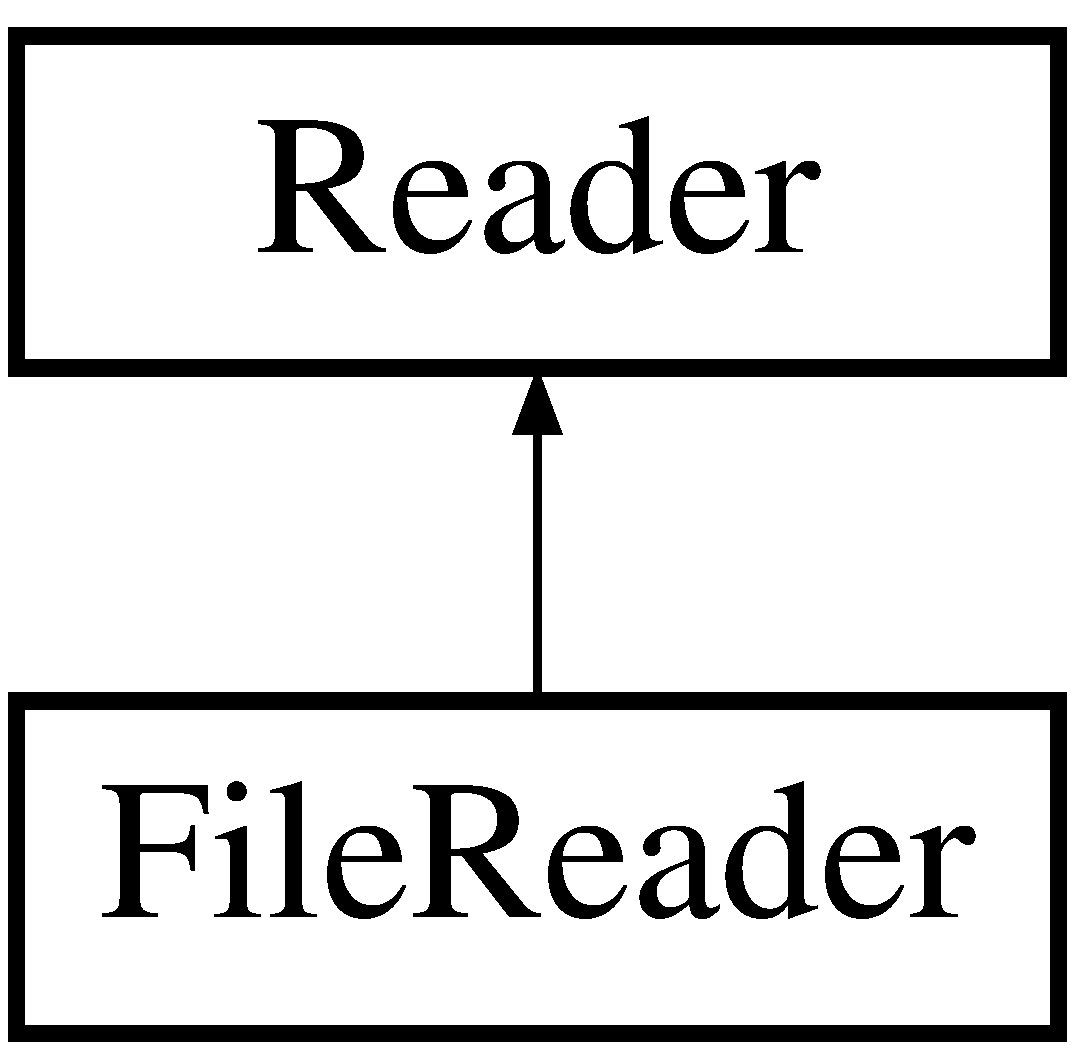
\includegraphics[height=2.000000cm]{classFileReader}
\end{center}
\end{figure}
\subsection*{Public Member Functions}
\begin{DoxyCompactItemize}
\item 
\hyperlink{classFileReader_a50ceae995b470d627f94caea10cd9956}{File\+Reader} (wstring file\+Name)
\begin{DoxyCompactList}\small\item\em Write what the function does here. \end{DoxyCompactList}\item 
\hypertarget{classFileReader_a3a06f152a16bd06550c3a4efeaed8ed2}{{\bfseries File\+Reader} (F\+I\+L\+E $\ast$f)}\label{classFileReader_a3a06f152a16bd06550c3a4efeaed8ed2}

\item 
virtual \hyperlink{classFileReader_a029d1ddebda388d1f0f5a99ce9acb311}{$\sim$\+File\+Reader} ()
\begin{DoxyCompactList}\small\item\em Write what the function does here. \end{DoxyCompactList}\item 
virtual uint8\+\_\+t \hyperlink{classFileReader_ac148435542dea9596532f2c3dd3c7668}{read\+Byte} () override
\begin{DoxyCompactList}\small\item\em Write what the function does here. \end{DoxyCompactList}\end{DoxyCompactItemize}
\subsection*{Private Attributes}
\begin{DoxyCompactItemize}
\item 
\hypertarget{classFileReader_a1a1ee8dcab91301260b9623e3b35b115}{F\+I\+L\+E $\ast$ {\bfseries f}}\label{classFileReader_a1a1ee8dcab91301260b9623e3b35b115}

\end{DoxyCompactItemize}


\subsection{Detailed Description}
Write what the function does here. 

\begin{DoxyReturn}{Returns}

\end{DoxyReturn}


Definition at line 804 of file stream.\+h.



\subsection{Constructor \& Destructor Documentation}
\hypertarget{classFileReader_a50ceae995b470d627f94caea10cd9956}{\index{File\+Reader@{File\+Reader}!File\+Reader@{File\+Reader}}
\index{File\+Reader@{File\+Reader}!File\+Reader@{File\+Reader}}
\subsubsection[{File\+Reader}]{\setlength{\rightskip}{0pt plus 5cm}File\+Reader\+::\+File\+Reader (
\begin{DoxyParamCaption}
\item[{wstring}]{file\+Name}
\end{DoxyParamCaption}
)\hspace{0.3cm}{\ttfamily [inline]}}}\label{classFileReader_a50ceae995b470d627f94caea10cd9956}


Write what the function does here. 


\begin{DoxyParams}{Parameters}
{\em file\+Name} & \\
\hline
\end{DoxyParams}
\begin{DoxyReturn}{Returns}

\end{DoxyReturn}


Definition at line 817 of file stream.\+h.


\begin{DoxyCode}
818         \{
819             \textcolor{keywordtype}{string} str = wstringToString(fileName);
820             f = fopen(str.c\_str(), \textcolor{stringliteral}{"rb"});
821             \textcolor{keywordflow}{if}(f == \textcolor{keyword}{nullptr})
822                 \textcolor{keywordflow}{throw} \hyperlink{classIOException}{IOException}(\textcolor{keywordtype}{string}(\textcolor{stringliteral}{"IO Error : "}) + strerror(errno));
823         \}
\end{DoxyCode}
\hypertarget{classFileReader_a029d1ddebda388d1f0f5a99ce9acb311}{\index{File\+Reader@{File\+Reader}!````~File\+Reader@{$\sim$\+File\+Reader}}
\index{````~File\+Reader@{$\sim$\+File\+Reader}!File\+Reader@{File\+Reader}}
\subsubsection[{$\sim$\+File\+Reader}]{\setlength{\rightskip}{0pt plus 5cm}virtual File\+Reader\+::$\sim$\+File\+Reader (
\begin{DoxyParamCaption}
{}
\end{DoxyParamCaption}
)\hspace{0.3cm}{\ttfamily [inline]}, {\ttfamily [virtual]}}}\label{classFileReader_a029d1ddebda388d1f0f5a99ce9acb311}


Write what the function does here. 

\begin{DoxyReturn}{Returns}

\end{DoxyReturn}


Definition at line 835 of file stream.\+h.


\begin{DoxyCode}
836         \{
837             fclose(f);
838         \}
\end{DoxyCode}


\subsection{Member Function Documentation}
\hypertarget{classFileReader_ac148435542dea9596532f2c3dd3c7668}{\index{File\+Reader@{File\+Reader}!read\+Byte@{read\+Byte}}
\index{read\+Byte@{read\+Byte}!File\+Reader@{File\+Reader}}
\subsubsection[{read\+Byte}]{\setlength{\rightskip}{0pt plus 5cm}virtual uint8\+\_\+t File\+Reader\+::read\+Byte (
\begin{DoxyParamCaption}
{}
\end{DoxyParamCaption}
)\hspace{0.3cm}{\ttfamily [inline]}, {\ttfamily [override]}, {\ttfamily [virtual]}}}\label{classFileReader_ac148435542dea9596532f2c3dd3c7668}


Write what the function does here. 

\begin{DoxyReturn}{Returns}

\end{DoxyReturn}


Implements \hyperlink{classReader}{Reader}.



Definition at line 845 of file stream.\+h.


\begin{DoxyCode}
846         \{
847             \textcolor{keywordtype}{int} ch = fgetc(f);
848 
849             \textcolor{keywordflow}{if}(ch == EOF)
850             \{
851                 \textcolor{keywordflow}{if}(ferror(f))
852                     \textcolor{keywordflow}{throw} \hyperlink{classIOException}{IOException}(\textcolor{stringliteral}{"IO Error : can't read from file"});
853                 \textcolor{keywordflow}{throw} \hyperlink{classEOFException}{EOFException}();
854             \}
855             \textcolor{keywordflow}{return} ch;
856         \}
\end{DoxyCode}


The documentation for this class was generated from the following file\+:\begin{DoxyCompactItemize}
\item 
stream.\+h\end{DoxyCompactItemize}

\hypertarget{classfinalizer}{\section{finalizer Class Reference}
\label{classfinalizer}\index{finalizer@{finalizer}}
}


Write what the function does here.  




{\ttfamily \#include $<$util.\+h$>$}

\subsection*{Public Member Functions}
\begin{DoxyCompactItemize}
\item 
\hypertarget{classfinalizer_abfb1a53ac8097489f7f832fab70ed438}{{\bfseries finalizer} (void($\ast$finalize\+Fn)())}\label{classfinalizer_abfb1a53ac8097489f7f832fab70ed438}

\item 
\hyperlink{classfinalizer_a5dd96a3bece0e0dc19686da3eeafbd0d}{$\sim$finalizer} ()
\begin{DoxyCompactList}\small\item\em Write what the function does here. \end{DoxyCompactList}\end{DoxyCompactItemize}
\subsection*{Private Member Functions}
\begin{DoxyCompactItemize}
\item 
\hypertarget{classfinalizer_ae13d210c53c985301d67b6744f6455de}{{\bfseries finalizer} (const \hyperlink{classfinalizer}{finalizer} \&rt)=delete}\label{classfinalizer_ae13d210c53c985301d67b6744f6455de}

\item 
\hypertarget{classfinalizer_aea0825760a746dad9f22299960bc83c8}{void {\bfseries operator=} (const \hyperlink{classfinalizer}{finalizer} \&rt)=delete}\label{classfinalizer_aea0825760a746dad9f22299960bc83c8}

\end{DoxyCompactItemize}
\subsection*{Private Attributes}
\begin{DoxyCompactItemize}
\item 
\hypertarget{classfinalizer_ac9a4efb8dc93d75de3fb6561ebb59d0a}{void($\ast$ {\bfseries finalize\+Fn} )()}\label{classfinalizer_ac9a4efb8dc93d75de3fb6561ebb59d0a}

\end{DoxyCompactItemize}


\subsection{Detailed Description}
Write what the function does here. 


\begin{DoxyRetVals}{Return values}
{\em (variable)} & (description of variable) \\
\hline
\end{DoxyRetVals}


Definition at line 147 of file util.\+h.



\subsection{Constructor \& Destructor Documentation}
\hypertarget{classfinalizer_a5dd96a3bece0e0dc19686da3eeafbd0d}{\index{finalizer@{finalizer}!````~finalizer@{$\sim$finalizer}}
\index{````~finalizer@{$\sim$finalizer}!finalizer@{finalizer}}
\subsubsection[{$\sim$finalizer}]{\setlength{\rightskip}{0pt plus 5cm}finalizer\+::$\sim$finalizer (
\begin{DoxyParamCaption}
{}
\end{DoxyParamCaption}
)\hspace{0.3cm}{\ttfamily [inline]}}}\label{classfinalizer_a5dd96a3bece0e0dc19686da3eeafbd0d}


Write what the function does here. 


\begin{DoxyRetVals}{Return values}
{\em (variable)} & (description of variable) \\
\hline
\end{DoxyRetVals}


Definition at line 165 of file util.\+h.


\begin{DoxyCode}
166         \{
167             finalizeFn();
168         \}
\end{DoxyCode}


The documentation for this class was generated from the following file\+:\begin{DoxyCompactItemize}
\item 
util.\+h\end{DoxyCompactItemize}

\hypertarget{structFlipTimeLocker}{\section{Flip\+Time\+Locker Struct Reference}
\label{structFlipTimeLocker}\index{Flip\+Time\+Locker@{Flip\+Time\+Locker}}
}


\subsection{Detailed Description}


Definition at line 364 of file platform.\+cpp.



The documentation for this struct was generated from the following file\+:\begin{DoxyCompactItemize}
\item 
platform.\+cpp\end{DoxyCompactItemize}

\hypertarget{classGame}{\section{Game Class Reference}
\label{classGame}\index{Game@{Game}}
}
Inheritance diagram for Game\+:\begin{figure}[H]
\begin{center}
\leavevmode
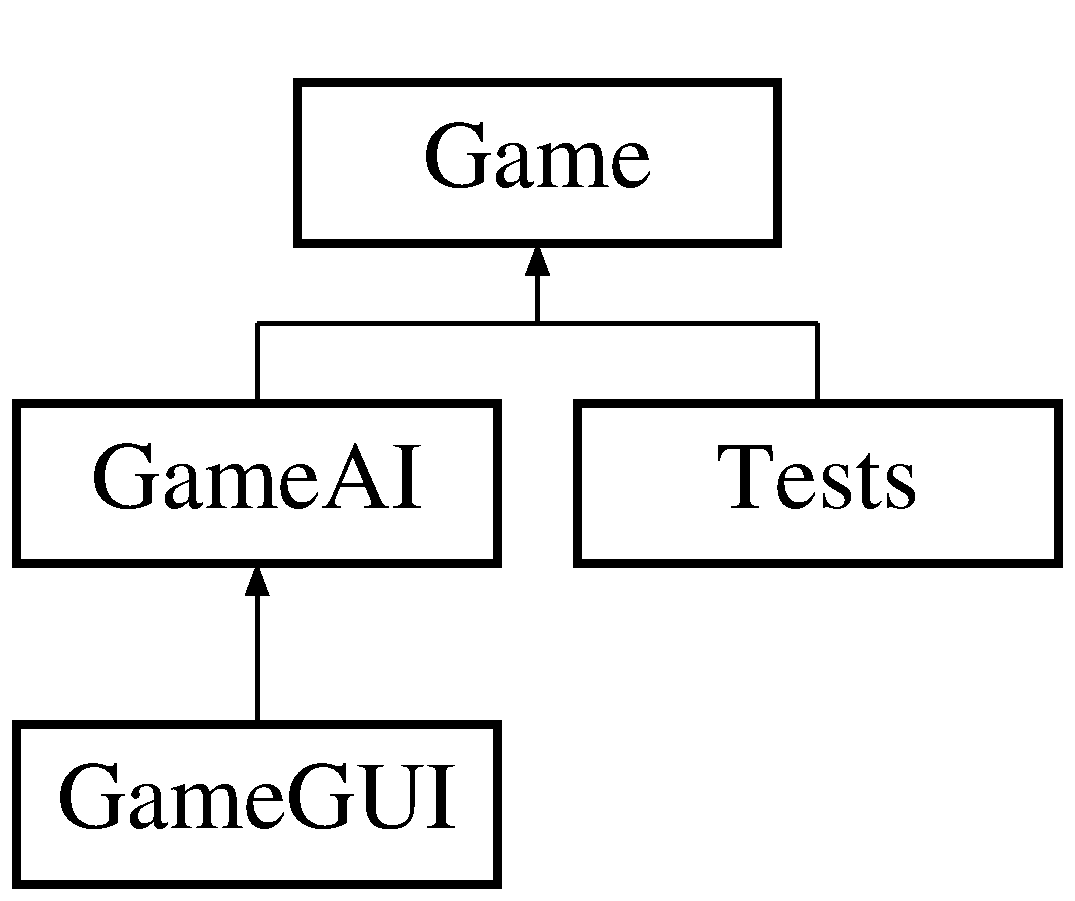
\includegraphics[height=3.000000cm]{classGame}
\end{center}
\end{figure}
\subsection*{Public Member Functions}
\begin{DoxyCompactItemize}
\item 
\hypertarget{classGame_aa79443880de5f26387c2a1c70c8c1aae}{{\bfseries Game} (const \hyperlink{classGame}{Game} \&)}\label{classGame_aa79443880de5f26387c2a1c70c8c1aae}

\item 
\hypertarget{classGame_aec1439ca4c76f4a002c235134d590158}{\hyperlink{classGame}{Game} \& {\bfseries operator=} (const \hyperlink{classGame}{Game} \&)}\label{classGame_aec1439ca4c76f4a002c235134d590158}

\item 
\hypertarget{classGame_a23882a4a63f1ea6c17bc6330440ff6f4}{void {\bfseries do\+Move} (const Line \&, \hyperlink{structCoord}{Coord} middle, bool extra\+Checks=false)}\label{classGame_a23882a4a63f1ea6c17bc6330440ff6f4}

\item 
\hypertarget{classGame_ac0652dbca9ce754f465cee5a81f508ae}{void {\bfseries update\+Areas} ()}\label{classGame_ac0652dbca9ce754f465cee5a81f508ae}

\item 
\hypertarget{classGame_a6134468ea7bb0bd23cc2b03a5f1a7e7c}{int {\bfseries moves} () const }\label{classGame_a6134468ea7bb0bd23cc2b03a5f1a7e7c}

\item 
\hypertarget{classGame_aa82304a9d084304f05ef8d8a6eeb732a}{bool {\bfseries connectable} (const \hyperlink{classNode}{Node} \&, const \hyperlink{classNode}{Node} \&) const }\label{classGame_aa82304a9d084304f05ef8d8a6eeb732a}

\item 
\hypertarget{classGame_a2c5aa5c26eb65e3f992701ac0408393e}{bool {\bfseries is\+In\+Area} (const Area \&, \hyperlink{structCoord}{Coord}) const }\label{classGame_a2c5aa5c26eb65e3f992701ac0408393e}

\item 
\hypertarget{classGame_a73b99aad84bf161b64ad012173528cfa}{bool {\bfseries game\+Ended} () const }\label{classGame_a73b99aad84bf161b64ad012173528cfa}

\item 
\hypertarget{classGame_ad377f36ff3fe304f6905f05427aa1ab2}{\hyperlink{classNode}{Node} \& {\bfseries insert\+Node} (\hyperlink{structCoord}{Coord}, \hyperlink{structConnection}{Connection}=\hyperlink{structConnection}{Connection}(), \hyperlink{structConnection}{Connection}=\hyperlink{structConnection}{Connection}())}\label{classGame_ad377f36ff3fe304f6905f05427aa1ab2}

\item 
\hypertarget{classGame_a25d65e35ad5efbd14c4dbe4476bb5ec0}{\hyperlink{classNode}{Node} $\ast$ {\bfseries find\+Node} (\hyperlink{structCoord}{Coord}) const }\label{classGame_a25d65e35ad5efbd14c4dbe4476bb5ec0}

\item 
\hypertarget{classGame_a8698d31d2f9314753f392dbd9bb13b3c}{Line \& {\bfseries insert\+Line} (const Line \&)}\label{classGame_a8698d31d2f9314753f392dbd9bb13b3c}

\end{DoxyCompactItemize}
\subsection*{Protected Attributes}
\begin{DoxyCompactItemize}
\item 
\hypertarget{classGame_a1ab0295c1555fa04614de7644d9999c3}{vector$<$ Areaset $\ast$ $>$ {\bfseries areasets}}\label{classGame_a1ab0295c1555fa04614de7644d9999c3}

\item 
\hypertarget{classGame_a21787871b15141dcf1cafeacbd68bc8c}{vector$<$ \hyperlink{classNode}{Node} $\ast$ $>$ {\bfseries nodes}}\label{classGame_a21787871b15141dcf1cafeacbd68bc8c}

\item 
\hypertarget{classGame_acef1deb6e1ef97d367afaeb04af5226c}{vector$<$ Line $\ast$ $>$ {\bfseries lines}}\label{classGame_acef1deb6e1ef97d367afaeb04af5226c}

\end{DoxyCompactItemize}
\subsection*{Private Member Functions}
\begin{DoxyCompactItemize}
\item 
\hypertarget{classGame_a961f632fbe7f4ba08d23fe9edc7711be}{void {\bfseries cleanup} ()}\label{classGame_a961f632fbe7f4ba08d23fe9edc7711be}

\item 
\hypertarget{classGame_a6334d9f0e04044e0fb711f32fe4cfac4}{void {\bfseries copy} (const \hyperlink{classGame}{Game} \&)}\label{classGame_a6334d9f0e04044e0fb711f32fe4cfac4}

\item 
\hypertarget{classGame_a18db1f732aa95c4c6d78440b6d4d109b}{void {\bfseries clear\+Areas} ()}\label{classGame_a18db1f732aa95c4c6d78440b6d4d109b}

\item 
\hypertarget{classGame_a53b0e200e4727eb76ba1bbbd44164c76}{void {\bfseries delete\+Last\+Node} ()}\label{classGame_a53b0e200e4727eb76ba1bbbd44164c76}

\end{DoxyCompactItemize}
\subsection*{Private Attributes}
\begin{DoxyCompactItemize}
\item 
\hypertarget{classGame_ad03a503539b01315b3fd020e148ff480}{bool {\bfseries updated}}\label{classGame_ad03a503539b01315b3fd020e148ff480}

\item 
\hypertarget{classGame_a3de2efa2690b73e5565fcd3f17ccbebc}{int {\bfseries move\+Count}}\label{classGame_a3de2efa2690b73e5565fcd3f17ccbebc}

\item 
\hypertarget{classGame_a75c85a025952d38a27db2b0b84206328}{vector$<$ Area $\ast$ $>$ {\bfseries areas}}\label{classGame_a75c85a025952d38a27db2b0b84206328}

\end{DoxyCompactItemize}
\subsection*{Friends}
\begin{DoxyCompactItemize}
\item 
\hypertarget{classGame_a7bb9176e07b6f6c73c930dba6400265f}{ostream \& {\bfseries operator$<$$<$} (ostream \&, const \hyperlink{classGame}{Game} \&)}\label{classGame_a7bb9176e07b6f6c73c930dba6400265f}

\end{DoxyCompactItemize}


\subsection{Detailed Description}


Definition at line 53 of file game.\+h.



The documentation for this class was generated from the following files\+:\begin{DoxyCompactItemize}
\item 
headers/game.\+h\item 
old-\/source/game.\+cpp\end{DoxyCompactItemize}

\hypertarget{classGameAI}{\section{Game\+A\+I Class Reference}
\label{classGameAI}\index{Game\+A\+I@{Game\+A\+I}}
}
Inheritance diagram for Game\+A\+I\+:\begin{figure}[H]
\begin{center}
\leavevmode
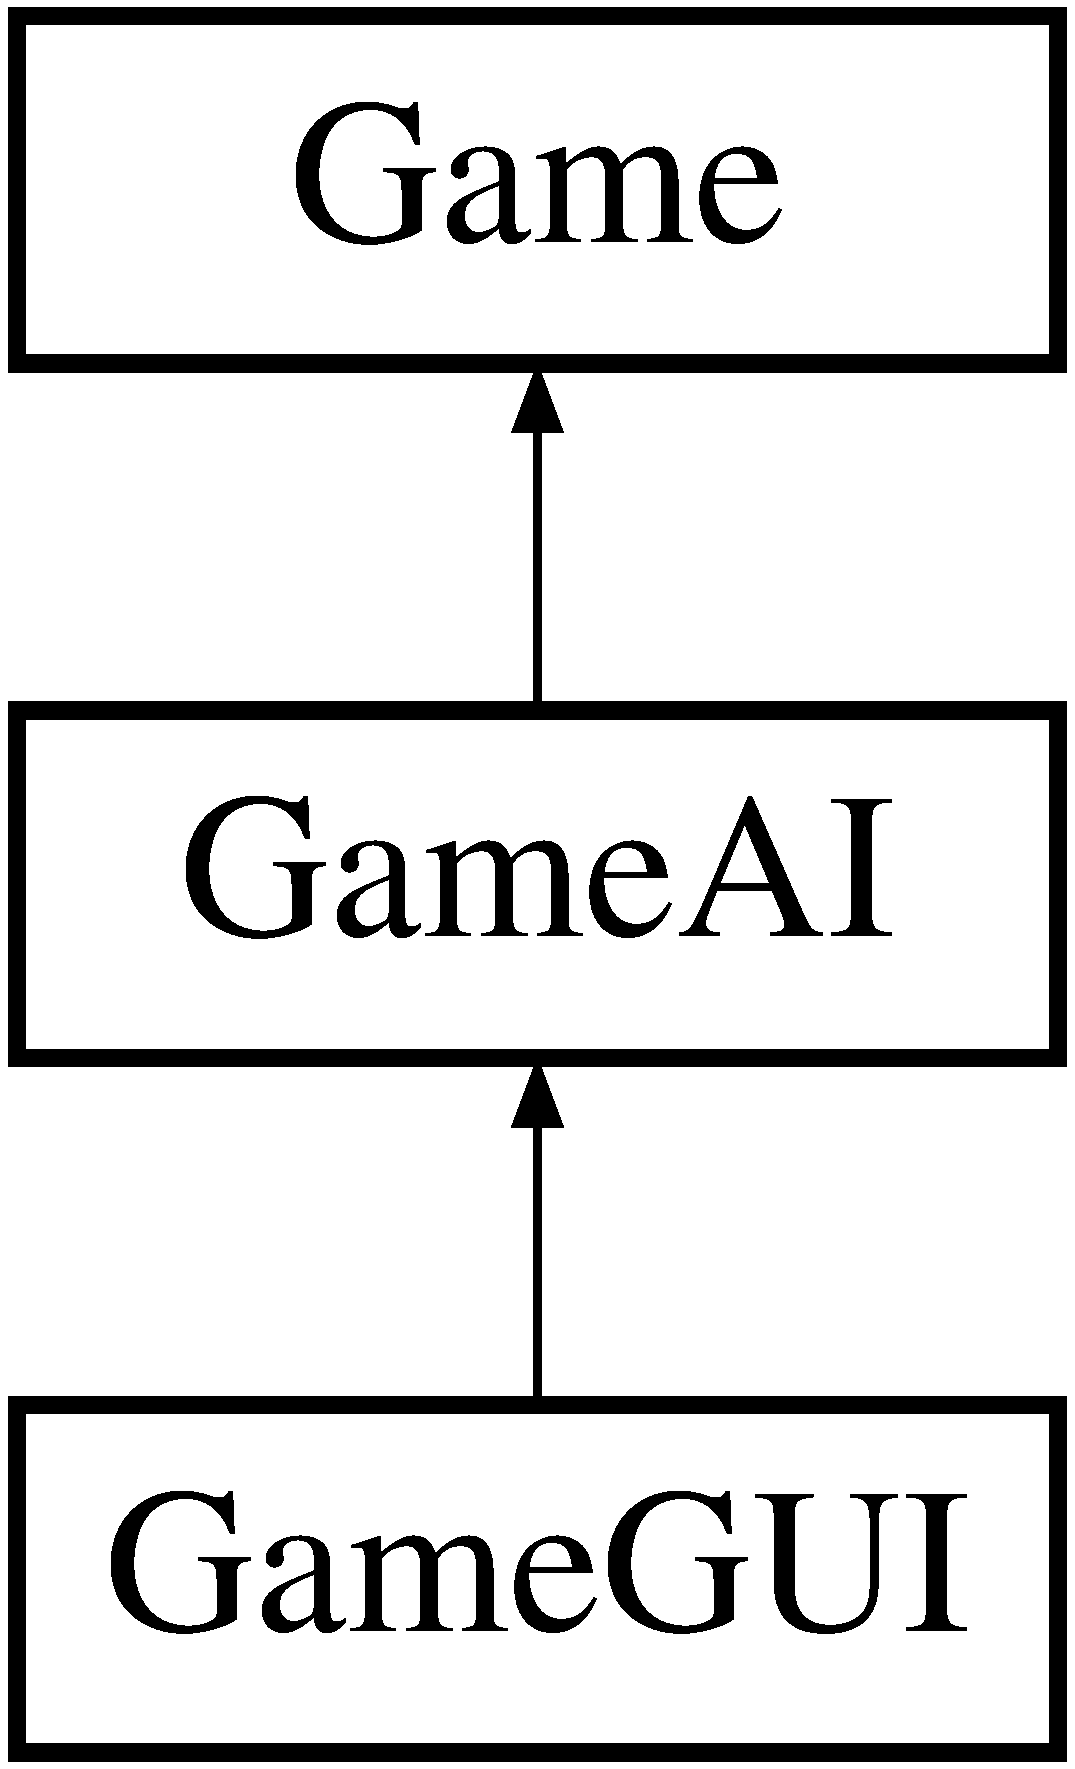
\includegraphics[height=3.000000cm]{classGameAI}
\end{center}
\end{figure}
\subsection*{Public Member Functions}
\begin{DoxyCompactItemize}
\item 
\hypertarget{classGameAI_ab36abdfff623feb9e4541c59752c2132}{int {\bfseries not\+Connectable\+Nodes} () const }\label{classGameAI_ab36abdfff623feb9e4541c59752c2132}

\item 
\hypertarget{classGameAI_a90f4924b104ca8a98b054cc4d12c779c}{void {\bfseries populate\+M\+List} ()}\label{classGameAI_a90f4924b104ca8a98b054cc4d12c779c}

\item 
\hypertarget{classGameAI_a12c06fd7a0c68da5af485e41048f0cc7}{bool {\bfseries ai\+Turn} ()}\label{classGameAI_a12c06fd7a0c68da5af485e41048f0cc7}

\item 
\hypertarget{classGameAI_afe0272443eed1a1392caf8c19380e502}{\hyperlink{structCoord}{Coord} {\bfseries mid\+Node} (const Line \&) const }\label{classGameAI_afe0272443eed1a1392caf8c19380e502}

\item 
\hypertarget{classGameAI_ad21315504d9b3bd4c00ce9effcd3909e}{Line {\bfseries create\+Line} (\hyperlink{classNode}{Node} $\ast$, \hyperlink{classNode}{Node} $\ast$) const }\label{classGameAI_ad21315504d9b3bd4c00ce9effcd3909e}

\item 
\hypertarget{classGameAI_a3f36972f212c2f0b65c03c0674d0383b}{bool {\bfseries required\+Areas} (bool, int) const }\label{classGameAI_a3f36972f212c2f0b65c03c0674d0383b}

\item 
\hypertarget{classGameAI_a4c6c1706af32bb21c81d8b5c2c4d37d9}{bool {\bfseries valid\+Single\+Line} (const Line \&, \hyperlink{structCoord}{Coord}, \hyperlink{structCoord}{Coord}) const }\label{classGameAI_a4c6c1706af32bb21c81d8b5c2c4d37d9}

\item 
\hypertarget{classGameAI_ac6a810b45dfec6db6d4f53f5c96106b3}{bool {\bfseries valid\+Line} (\hyperlink{structCoord}{Coord}, \hyperlink{structCoord}{Coord}) const }\label{classGameAI_ac6a810b45dfec6db6d4f53f5c96106b3}

\item 
\hypertarget{classGameAI_a2683127876773a7aa917deefe8ba6eeb}{bool {\bfseries valid\+Line} (\hyperlink{structCoord}{Coord}, \hyperlink{structCoord}{Coord}, bool) const }\label{classGameAI_a2683127876773a7aa917deefe8ba6eeb}

\item 
\hypertarget{classGameAI_ac49f4598c7f141ee226cc83e59c1c61d}{double {\bfseries distance} (\hyperlink{structCoord}{Coord} a, \hyperlink{structCoord}{Coord} b) const }\label{classGameAI_ac49f4598c7f141ee226cc83e59c1c61d}

\end{DoxyCompactItemize}
\subsection*{Protected Attributes}
\begin{DoxyCompactItemize}
\item 
\hypertarget{classGameAI_a50568e8c64c0a8f3f6c54f26acc13d99}{int {\bfseries starting\+Nodes}}\label{classGameAI_a50568e8c64c0a8f3f6c54f26acc13d99}

\item 
\hypertarget{classGameAI_a24a47307a58f64a84b62645b449df9bd}{vector$<$ Line $>$ {\bfseries possible\+Moves}}\label{classGameAI_a24a47307a58f64a84b62645b449df9bd}

\item 
\hypertarget{classGameAI_a8b76334b18d881864e744fe903685d62}{int {\bfseries test\+Unuseable\+Nodes}}\label{classGameAI_a8b76334b18d881864e744fe903685d62}

\item 
\hypertarget{classGameAI_ac81540eb7691f8e2f69f36e533c65125}{int {\bfseries wanted\+Areas}}\label{classGameAI_ac81540eb7691f8e2f69f36e533c65125}

\item 
\hypertarget{classGameAI_adbcfaf523749716aabb2a623d519f309}{bool {\bfseries ai\+First}}\label{classGameAI_adbcfaf523749716aabb2a623d519f309}

\end{DoxyCompactItemize}


\subsection{Detailed Description}


Definition at line 15 of file gameai.\+h.



The documentation for this class was generated from the following files\+:\begin{DoxyCompactItemize}
\item 
headers/gameai.\+h\item 
old-\/source/gameai.\+cpp\end{DoxyCompactItemize}

\hypertarget{classGameGUI}{\section{Game\+G\+U\+I Class Reference}
\label{classGameGUI}\index{Game\+G\+U\+I@{Game\+G\+U\+I}}
}
Inheritance diagram for Game\+G\+U\+I\+:\begin{figure}[H]
\begin{center}
\leavevmode
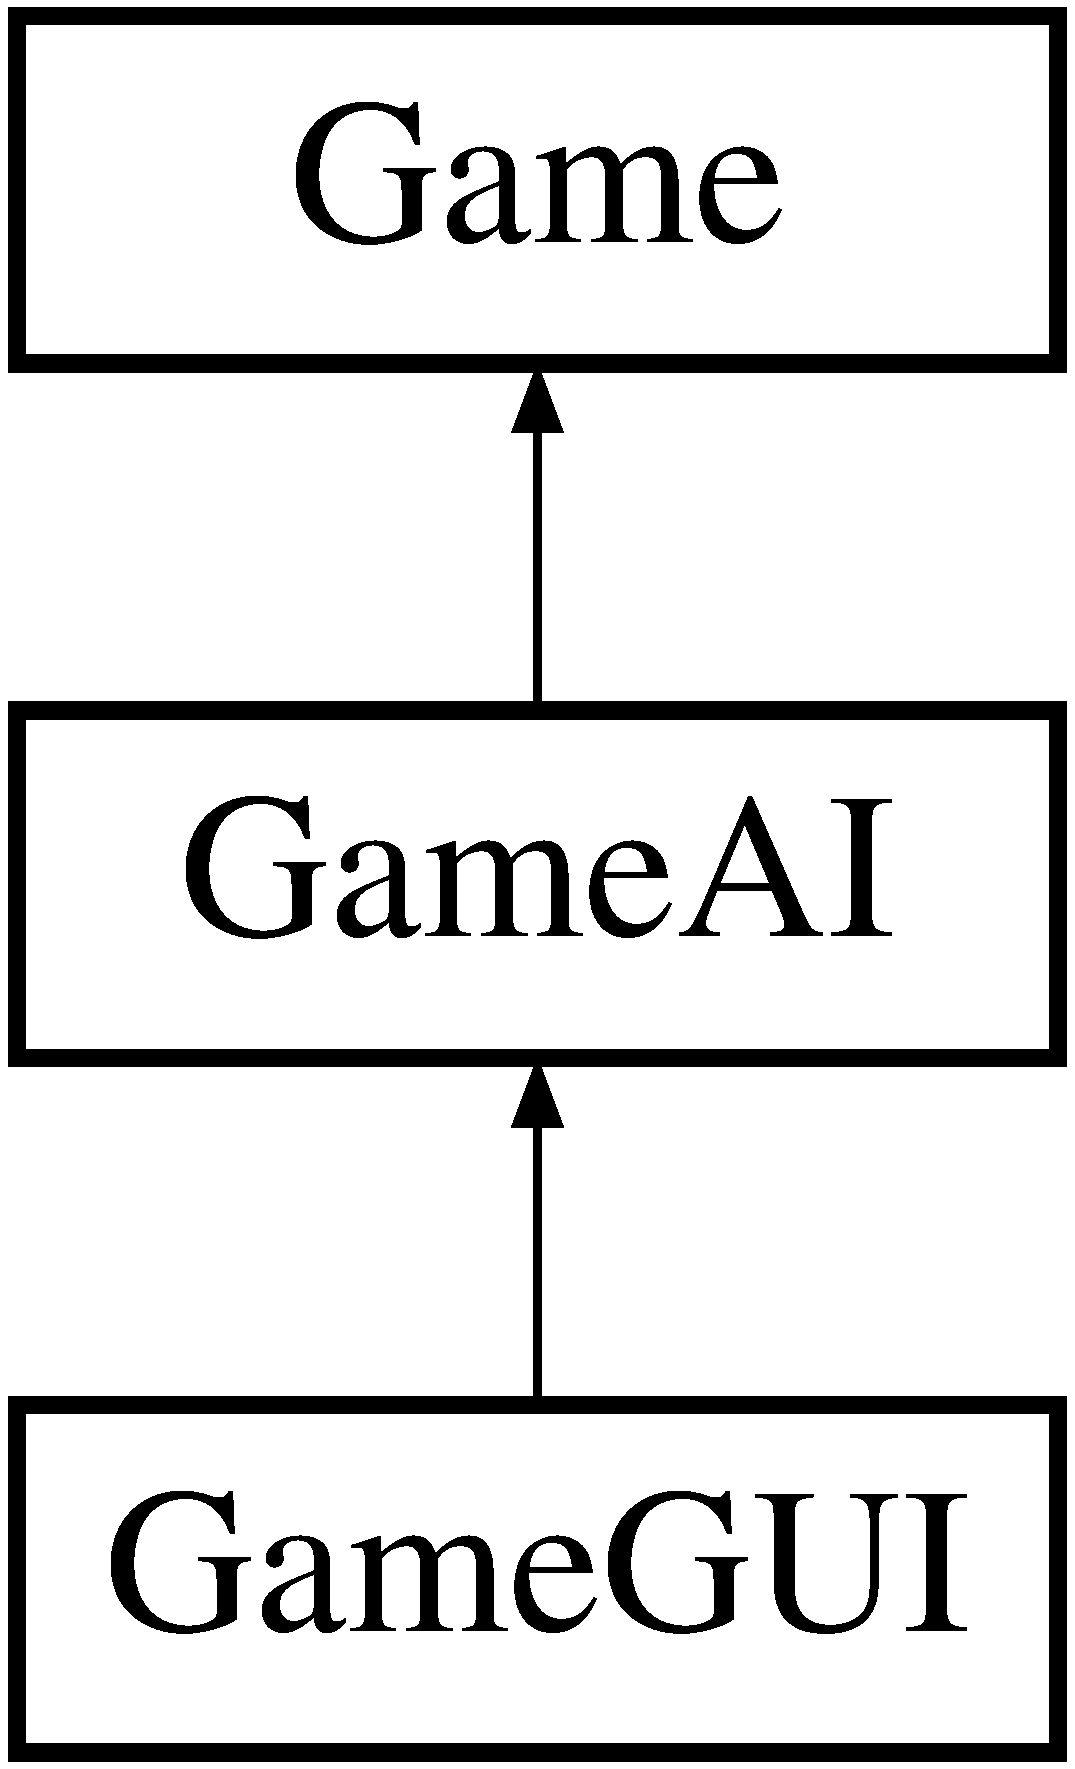
\includegraphics[height=3.000000cm]{classGameGUI}
\end{center}
\end{figure}
\subsection*{Public Member Functions}
\begin{DoxyCompactItemize}
\item 
\hypertarget{classGameGUI_a861b8dfdb3581b45689347f1d29dbaa4}{{\bfseries Game\+G\+U\+I} (\hyperlink{structSDL__Surface}{S\+D\+L\+\_\+\+Surface} $\ast$, T\+T\+F\+\_\+\+Font $\ast$)}\label{classGameGUI_a861b8dfdb3581b45689347f1d29dbaa4}

\item 
\hypertarget{classGameGUI_af64590a0f2446d0f423740f2b029ec38}{void {\bfseries init} (Mode, int, int, int)}\label{classGameGUI_af64590a0f2446d0f423740f2b029ec38}

\item 
\hypertarget{classGameGUI_a3b7fac84cc6dea53b4737f04d6c811bc}{void {\bfseries cancel} ()}\label{classGameGUI_a3b7fac84cc6dea53b4737f04d6c811bc}

\item 
\hypertarget{classGameGUI_a871d45a08bc3ccd49c81a4457bc816ca}{State {\bfseries click} (\hyperlink{structCoord}{Coord})}\label{classGameGUI_a871d45a08bc3ccd49c81a4457bc816ca}

\item 
\hypertarget{classGameGUI_aba9fcea825313750c6d20b6997d98acf}{void {\bfseries cursor} (\hyperlink{structCoord}{Coord})}\label{classGameGUI_aba9fcea825313750c6d20b6997d98acf}

\item 
\hypertarget{classGameGUI_aef1f54246657ec24df74b1fb70745e33}{bool {\bfseries player\+Turn} () const }\label{classGameGUI_aef1f54246657ec24df74b1fb70745e33}

\end{DoxyCompactItemize}
\subsection*{Public Attributes}
\begin{DoxyCompactItemize}
\item 
\hypertarget{classGameGUI_ae406bf29c4d36199bc57cf421b4216f6}{bool {\bfseries player1}}\label{classGameGUI_ae406bf29c4d36199bc57cf421b4216f6}

\item 
\hypertarget{classGameGUI_a5b2ce95070adc6cb2ca2b9456e63f4e2}{bool {\bfseries error}}\label{classGameGUI_a5b2ce95070adc6cb2ca2b9456e63f4e2}

\end{DoxyCompactItemize}
\subsection*{Private Member Functions}
\begin{DoxyCompactItemize}
\item 
\hypertarget{classGameGUI_a592ace24e5d51ac5a199b58be854eb46}{\hyperlink{structCoord}{Coord} {\bfseries center} () const }\label{classGameGUI_a592ace24e5d51ac5a199b58be854eb46}

\item 
\hypertarget{classGameGUI_ae55b18a0f3d6fc2e03544ec77358482c}{void {\bfseries lock} ()}\label{classGameGUI_ae55b18a0f3d6fc2e03544ec77358482c}

\item 
\hypertarget{classGameGUI_a0aa550e8ebc5ac6f93183edfd95fe471}{void {\bfseries unlock} ()}\label{classGameGUI_a0aa550e8ebc5ac6f93183edfd95fe471}

\item 
\hypertarget{classGameGUI_a319990b62283916ac319e703b8be1310}{void {\bfseries redraw} (bool lock\+\_\+screen=true)}\label{classGameGUI_a319990b62283916ac319e703b8be1310}

\item 
\hypertarget{classGameGUI_a875b89ee8751d94293bf329c9b759517}{void {\bfseries line} (\hyperlink{structCoord}{Coord}, \hyperlink{structCoord}{Coord}, Uint32 color)}\label{classGameGUI_a875b89ee8751d94293bf329c9b759517}

\item 
\hypertarget{classGameGUI_a49925f8ecdd22519d668b28d79badeb2}{void {\bfseries circle} (\hyperlink{structCoord}{Coord}, int radius, Uint32 color)}\label{classGameGUI_a49925f8ecdd22519d668b28d79badeb2}

\item 
\hypertarget{classGameGUI_aa2ecb2062a00e6d7e099fe0fd706313c}{bool {\bfseries valid\+Line} (\hyperlink{structCoord}{Coord}, \hyperlink{structCoord}{Coord}, bool) const }\label{classGameGUI_aa2ecb2062a00e6d7e099fe0fd706313c}

\item 
\hypertarget{classGameGUI_af786a5df1b7ae2d2d0309cda34d30c3c}{bool {\bfseries valid\+Single\+Line} (const Line \&, \hyperlink{structCoord}{Coord}, \hyperlink{structCoord}{Coord}, int, bool) const }\label{classGameGUI_af786a5df1b7ae2d2d0309cda34d30c3c}

\item 
\hypertarget{classGameGUI_aad8d3da450b57b150be4fc1c24594f47}{bool {\bfseries vertical} (\hyperlink{structCoord}{Coord}, \hyperlink{structCoord}{Coord}) const }\label{classGameGUI_aad8d3da450b57b150be4fc1c24594f47}

\item 
\hypertarget{classGameGUI_a12816d2f7a5043a03242186968a7c098}{\hyperlink{structCoord}{Coord} {\bfseries straighten} (\hyperlink{structCoord}{Coord} last, \hyperlink{structCoord}{Coord} point) const }\label{classGameGUI_a12816d2f7a5043a03242186968a7c098}

\item 
\hypertarget{classGameGUI_a4900be71f21cecf0aafca9d9201b7c77}{\hyperlink{structCoord}{Coord} {\bfseries firststraighten} (\hyperlink{structCoord}{Coord}, \hyperlink{structCoord}{Coord}, bool, bool, bool, bool) const }\label{classGameGUI_a4900be71f21cecf0aafca9d9201b7c77}

\item 
\hypertarget{classGameGUI_aa12fbbd12f46981f02e78fbfd2a5d404}{void {\bfseries combine\+Lines} (\hyperlink{structCoord}{Coord})}\label{classGameGUI_aa12fbbd12f46981f02e78fbfd2a5d404}

\item 
\hypertarget{classGameGUI_ada539abb78b785c11172aa9bf4dfabf6}{double {\bfseries distance} (\hyperlink{structCoord}{Coord}, \hyperlink{structCoord}{Coord}) const }\label{classGameGUI_ada539abb78b785c11172aa9bf4dfabf6}

\item 
\hypertarget{classGameGUI_ac927454c0511580c102ddc739fd9a6df}{\hyperlink{structNode}{Node} $\ast$ {\bfseries selected\+Node} (\hyperlink{structCoord}{Coord}) const }\label{classGameGUI_ac927454c0511580c102ddc739fd9a6df}

\item 
\hypertarget{classGameGUI_a597ba4a997c9aca9d765ce1b43613001}{\hyperlink{structCoord}{Coord} {\bfseries find\+Middle} () const }\label{classGameGUI_a597ba4a997c9aca9d765ce1b43613001}

\item 
\hypertarget{classGameGUI_a346606e8f741b3fad9d9fcccdd4b4a5b}{void {\bfseries display\+Position} (\hyperlink{structCoord}{Coord})}\label{classGameGUI_a346606e8f741b3fad9d9fcccdd4b4a5b}

\item 
\hypertarget{classGameGUI_a414dd5716a93388919d89ca82ffb1d23}{void {\bfseries display\+Error} (const string \&)}\label{classGameGUI_a414dd5716a93388919d89ca82ffb1d23}

\end{DoxyCompactItemize}
\subsection*{Private Attributes}
\begin{DoxyCompactItemize}
\item 
\hypertarget{classGameGUI_a36d66af3091c9d98a68c07635ed3d7d1}{\hyperlink{structSDL__Surface}{S\+D\+L\+\_\+\+Surface} $\ast$ {\bfseries screen}}\label{classGameGUI_a36d66af3091c9d98a68c07635ed3d7d1}

\item 
\hypertarget{classGameGUI_a299611c20e79f1a1201c286b3ccafef0}{T\+T\+F\+\_\+\+Font $\ast$ {\bfseries font}}\label{classGameGUI_a299611c20e79f1a1201c286b3ccafef0}

\item 
\hypertarget{classGameGUI_a0f821145e9fe953efd2a17050a943d3b}{Mode {\bfseries player\+Mode}}\label{classGameGUI_a0f821145e9fe953efd2a17050a943d3b}

\item 
\hypertarget{classGameGUI_a5edf0cb0d35c985f80ae9537fd25ae55}{State {\bfseries state}}\label{classGameGUI_a5edf0cb0d35c985f80ae9537fd25ae55}

\item 
\hypertarget{classGameGUI_a3dfe0ccdd1468a7dc735db9ac7e8f55b}{Line {\bfseries current\+Line}}\label{classGameGUI_a3dfe0ccdd1468a7dc735db9ac7e8f55b}

\item 
\hypertarget{classGameGUI_aae17f26d90497475d50c65a8000cb181}{\hyperlink{structSDL__Color}{S\+D\+L\+\_\+\+Color} {\bfseries text\+Col}}\label{classGameGUI_aae17f26d90497475d50c65a8000cb181}

\item 
\hypertarget{classGameGUI_a075d8943a94366ce096941cab4e0264c}{int {\bfseries node\+Radius}}\label{classGameGUI_a075d8943a94366ce096941cab4e0264c}

\item 
\hypertarget{classGameGUI_a34ec0729523dfd0b80214071274a59e9}{int {\bfseries line\+Thick}}\label{classGameGUI_a34ec0729523dfd0b80214071274a59e9}

\end{DoxyCompactItemize}
\subsection*{Static Private Attributes}
\begin{DoxyCompactItemize}
\item 
\hypertarget{classGameGUI_a3538fd5d42ac59248b1a83d5f43fad0c}{static const Uint32 {\bfseries node\+Col} = 0x\+F\+F4500\+F\+F}\label{classGameGUI_a3538fd5d42ac59248b1a83d5f43fad0c}

\item 
\hypertarget{classGameGUI_ab0bebe6620cd6172be5897a42a0dcacb}{static const Uint32 {\bfseries line\+Col} = 0x\+F\+F\+F\+F\+F\+F\+F\+F}\label{classGameGUI_ab0bebe6620cd6172be5897a42a0dcacb}

\item 
\hypertarget{classGameGUI_af35f33e73362109de3751e0478c36cee}{static const Uint32 {\bfseries player1\+Col} = 0x069\+D\+D6\+F\+F}\label{classGameGUI_af35f33e73362109de3751e0478c36cee}

\item 
\hypertarget{classGameGUI_aca95044a11eb45ba6aee9c6842a4afb4}{static const Uint32 {\bfseries player2\+Col} = 0x\+F\+E0208\+F\+F}\label{classGameGUI_aca95044a11eb45ba6aee9c6842a4afb4}

\end{DoxyCompactItemize}
\subsection*{Additional Inherited Members}


\subsection{Detailed Description}


Definition at line 28 of file gamegui.\+h.



The documentation for this class was generated from the following files\+:\begin{DoxyCompactItemize}
\item 
headers/gamegui.\+h\item 
old-\/source/gamegui.\+cpp\end{DoxyCompactItemize}

\hypertarget{classgraph}{\section{graph$<$ N\+T, E\+T $>$ Class Template Reference}
\label{classgraph}\index{graph$<$ N\+T, E\+T $>$@{graph$<$ N\+T, E\+T $>$}}
}


Write what the function does here.  




{\ttfamily \#include $<$graph.\+h$>$}

\subsection*{Classes}
\begin{DoxyCompactItemize}
\item 
struct \hyperlink{structgraph_1_1Edge}{Edge}
\begin{DoxyCompactList}\small\item\em Write what the function does here. \end{DoxyCompactList}\item 
class \hyperlink{classgraph_1_1edge__iterator}{edge\+\_\+iterator}
\item 
struct \hyperlink{structgraph_1_1Node}{Node}
\begin{DoxyCompactList}\small\item\em Write what the function does here. \end{DoxyCompactList}\item 
class \hyperlink{classgraph_1_1node__iterator}{node\+\_\+iterator}
\begin{DoxyCompactList}\small\item\em Write what the function does here. \end{DoxyCompactList}\end{DoxyCompactItemize}
\subsection*{Public Member Functions}
\begin{DoxyCompactItemize}
\item 
\hyperlink{classgraph_af87b66e0c5abea18db06492c14adb5fb}{graph} ()
\begin{DoxyCompactList}\small\item\em Write what the function does here. \end{DoxyCompactList}\item 
\hyperlink{classgraph_a86a49b0dd6f2fbbdab4a044bb29e4a2a}{$\sim$graph} ()
\begin{DoxyCompactList}\small\item\em Write what the function does here. \end{DoxyCompactList}\item 
\hyperlink{classgraph_a0544402982f793695fb9cc071600b4b9}{graph} (const \hyperlink{classgraph}{graph} \&rt)
\begin{DoxyCompactList}\small\item\em Write what the function does here. \end{DoxyCompactList}\item 
\hyperlink{classgraph_a9353a5e27c35250f323b6f2bf7c14c40}{graph} (\hyperlink{classgraph}{graph} \&\&rt)
\begin{DoxyCompactList}\small\item\em Write what the function does here. \end{DoxyCompactList}\item 
const \hyperlink{classgraph}{graph} \& \hyperlink{classgraph_a08ffaf262ac16616c296d1b3c3c31559}{operator=} (\hyperlink{classgraph}{graph} \&\&rt)
\begin{DoxyCompactList}\small\item\em Write what the function does here. \end{DoxyCompactList}\item 
const \hyperlink{classgraph}{graph} \& \hyperlink{classgraph_aeb9dc4e35433477ab6c722eedaefd293}{operator=} (const \hyperlink{classgraph}{graph} \&rt)
\begin{DoxyCompactList}\small\item\em Write what the function does here. \end{DoxyCompactList}\item 
\hyperlink{classgraph_1_1node__iterator}{node\+\_\+iterator} \hyperlink{classgraph_a48e506355f6373565ba7578f23ee3d41}{begin} () const 
\begin{DoxyCompactList}\small\item\em Write what the function does here. \end{DoxyCompactList}\item 
\hyperlink{classgraph_1_1node__iterator}{node\+\_\+iterator} \hyperlink{classgraph_aa4af57bdee2a19b491b3113db848b4a9}{cbegin} () const 
\begin{DoxyCompactList}\small\item\em Write what the function does here. \end{DoxyCompactList}\item 
\hyperlink{classgraph_1_1node__iterator}{node\+\_\+iterator} \hyperlink{classgraph_a4ddb1dc38890533ccb8385909c834b8e}{end} () const 
\begin{DoxyCompactList}\small\item\em Write what the function does here. \end{DoxyCompactList}\item 
\hyperlink{classgraph_1_1node__iterator}{node\+\_\+iterator} \hyperlink{classgraph_ab15637ab99f3448d53c38ecc51d1dcd3}{cend} () const 
\begin{DoxyCompactList}\small\item\em Write what the function does here. \end{DoxyCompactList}\item 
\hyperlink{classgraph_1_1edge__iterator}{edge\+\_\+iterator} \hyperlink{classgraph_a999ee39b5e84843292a3737bdd32739b}{begin} (\hyperlink{classgraph_1_1node__iterator}{node\+\_\+iterator} ni) const 
\begin{DoxyCompactList}\small\item\em Write what the function does here. \end{DoxyCompactList}\item 
\hyperlink{classgraph_1_1edge__iterator}{edge\+\_\+iterator} \hyperlink{classgraph_ac5165defe7702d8c55fdb72ecb5b6444}{cbegin} (\hyperlink{classgraph_1_1node__iterator}{node\+\_\+iterator} ni) const 
\begin{DoxyCompactList}\small\item\em Write what the function does here. \end{DoxyCompactList}\item 
\hyperlink{classgraph_1_1edge__iterator}{edge\+\_\+iterator} \hyperlink{classgraph_ad7837541f30edcae34922ffe4dbbcf7a}{end} (\hyperlink{classgraph_1_1node__iterator}{node\+\_\+iterator} ni) const 
\begin{DoxyCompactList}\small\item\em Write what the function does here. \end{DoxyCompactList}\item 
\hyperlink{classgraph_1_1edge__iterator}{edge\+\_\+iterator} \hyperlink{classgraph_a7165be7146a4f54364b3b6060af2f42a}{cend} (\hyperlink{classgraph_1_1node__iterator}{node\+\_\+iterator} ni) const 
\begin{DoxyCompactList}\small\item\em Write what the function does here. \end{DoxyCompactList}\item 
bool \hyperlink{classgraph_aaec1657b0786d291b8ec3e916c888ddd}{is\+Graph\+Connected\+Depth\+First} () const 
\begin{DoxyCompactList}\small\item\em Write what the function does here. \end{DoxyCompactList}\item 
bool \hyperlink{classgraph_ad5fac5d1e968a1fd89e816e9c320b05f}{is\+Graph\+Connected\+Breadth\+First} () const 
\begin{DoxyCompactList}\small\item\em Write what the function does here. \end{DoxyCompactList}\item 
\hyperlink{classgraph_1_1node__iterator}{node\+\_\+iterator} \hyperlink{classgraph_a8465347e19dc13e8685c33cd71738a80}{add\+Node} (const N\+T \&data)
\begin{DoxyCompactList}\small\item\em Write what the function does here. \end{DoxyCompactList}\item 
\hyperlink{classgraph_1_1node__iterator}{node\+\_\+iterator} \hyperlink{classgraph_a2417ef9e682bf1ed4ab3c6d3c0b4dac4}{add\+Node} (N\+T \&\&data)
\begin{DoxyCompactList}\small\item\em Write what the function does here. \end{DoxyCompactList}\item 
bool \hyperlink{classgraph_a8db619fbe866a5082fb675039f650e7f}{has\+Edge} (\hyperlink{classgraph_1_1node__iterator}{node\+\_\+iterator} src, \hyperlink{classgraph_1_1node__iterator}{node\+\_\+iterator} dest) const 
\begin{DoxyCompactList}\small\item\em Write what the function does here. \end{DoxyCompactList}\item 
\hyperlink{classgraph_1_1edge__iterator}{edge\+\_\+iterator} \hyperlink{classgraph_a6a92c77420e9cfc42a54585be4015e6b}{add\+Edge} (const E\+T \&data, \hyperlink{classgraph_1_1node__iterator}{node\+\_\+iterator} src, \hyperlink{classgraph_1_1node__iterator}{node\+\_\+iterator} dest)
\begin{DoxyCompactList}\small\item\em Write what the function does here. \end{DoxyCompactList}\item 
\hyperlink{classgraph_1_1edge__iterator}{edge\+\_\+iterator} \hyperlink{classgraph_a0806e4b7471c184dff54810cc42affa2}{add\+Edge} (E\+T \&\&data, \hyperlink{classgraph_1_1node__iterator}{node\+\_\+iterator} src, \hyperlink{classgraph_1_1node__iterator}{node\+\_\+iterator} dest)
\begin{DoxyCompactList}\small\item\em Write what the function does here. \end{DoxyCompactList}\item 
size\+\_\+t \hyperlink{classgraph_a6a3e81c21b51b8575a5f47e0b2dcab20}{node\+Count} () const 
\begin{DoxyCompactList}\small\item\em Write what the function does here. \end{DoxyCompactList}\item 
size\+\_\+t \hyperlink{classgraph_a83ef554d61963a3ac05ab1a1d052aad9}{edge\+Count} () const 
\begin{DoxyCompactList}\small\item\em Write what the function does here. \end{DoxyCompactList}\end{DoxyCompactItemize}
\subsection*{Private Member Functions}
\begin{DoxyCompactItemize}
\item 
void \hyperlink{classgraph_ac745949ed8867e94ca254905f6fd6194}{is\+Graph\+Connected\+Depth\+First\+Helper} (\hyperlink{structgraph_1_1Node}{Node} $\ast$node) const 
\begin{DoxyCompactList}\small\item\em Write what the function does here. \end{DoxyCompactList}\item 
bool \hyperlink{classgraph_a54e520186fad4c7e75912932910ef0c6}{any\+Flag\+Matches} (bool state) const 
\begin{DoxyCompactList}\small\item\em Write what the function does here. \end{DoxyCompactList}\item 
bool \hyperlink{classgraph_a14b48e6c76549fe5faff1ea51ec78fb3}{any\+Marked} () const 
\begin{DoxyCompactList}\small\item\em Write what the function does here. \end{DoxyCompactList}\item 
bool \hyperlink{classgraph_ab65c298ca639f7293459af9038920c6d}{all\+Marked} () const 
\begin{DoxyCompactList}\small\item\em Write what the function does here. \end{DoxyCompactList}\end{DoxyCompactItemize}
\subsection*{Private Attributes}
\begin{DoxyCompactItemize}
\item 
\hypertarget{classgraph_ac106879f6e370243b2413de2a0504da4}{vector$<$ \hyperlink{structgraph_1_1Node}{Node} $\ast$ $>$ {\bfseries nodes}}\label{classgraph_ac106879f6e370243b2413de2a0504da4}

\item 
\hypertarget{classgraph_a52ef68305fa541a124199c0e6283b46d}{vector$<$ \hyperlink{structgraph_1_1Edge}{Edge} $\ast$ $>$ {\bfseries edges}}\label{classgraph_a52ef68305fa541a124199c0e6283b46d}

\end{DoxyCompactItemize}
\subsection*{Friends}
\begin{DoxyCompactItemize}
\item 
\hypertarget{classgraph_a3f17ad3ab403d6cde1e4d08908bcdb52}{{\footnotesize template$<$typename N\+T2 , typename E\+T2 $>$ }\\ostream \& {\bfseries operator$<$$<$} (ostream \&os, const \hyperlink{classgraph}{graph}$<$ N\+T2, E\+T2 $>$ \&g)}\label{classgraph_a3f17ad3ab403d6cde1e4d08908bcdb52}

\end{DoxyCompactItemize}


\subsection{Detailed Description}
\subsubsection*{template$<$typename N\+T, typename E\+T = N\+T$>$class graph$<$ N\+T, E\+T $>$}

Write what the function does here. 

class for a directed graph \begin{DoxyReturn}{Returns}

\end{DoxyReturn}


Definition at line 41 of file graph.\+h.



\subsection{Constructor \& Destructor Documentation}
\hypertarget{classgraph_af87b66e0c5abea18db06492c14adb5fb}{\index{graph@{graph}!graph@{graph}}
\index{graph@{graph}!graph@{graph}}
\subsubsection[{graph}]{\setlength{\rightskip}{0pt plus 5cm}template$<$typename N\+T , typename E\+T  = N\+T$>$ {\bf graph}$<$ N\+T, E\+T $>$\+::{\bf graph} (
\begin{DoxyParamCaption}
{}
\end{DoxyParamCaption}
)\hspace{0.3cm}{\ttfamily [inline]}}}\label{classgraph_af87b66e0c5abea18db06492c14adb5fb}


Write what the function does here. 

\begin{DoxyReturn}{Returns}

\end{DoxyReturn}


Definition at line 96 of file graph.\+h.


\begin{DoxyCode}
97         \{
98         \}
\end{DoxyCode}
\hypertarget{classgraph_a86a49b0dd6f2fbbdab4a044bb29e4a2a}{\index{graph@{graph}!````~graph@{$\sim$graph}}
\index{````~graph@{$\sim$graph}!graph@{graph}}
\subsubsection[{$\sim$graph}]{\setlength{\rightskip}{0pt plus 5cm}template$<$typename N\+T , typename E\+T  = N\+T$>$ {\bf graph}$<$ N\+T, E\+T $>$\+::$\sim${\bf graph} (
\begin{DoxyParamCaption}
{}
\end{DoxyParamCaption}
)\hspace{0.3cm}{\ttfamily [inline]}}}\label{classgraph_a86a49b0dd6f2fbbdab4a044bb29e4a2a}


Write what the function does here. 

\begin{DoxyReturn}{Returns}

\end{DoxyReturn}


Definition at line 105 of file graph.\+h.


\begin{DoxyCode}
106         \{
107 
108             \textcolor{keywordflow}{for}(\hyperlink{classNode}{Node} *node : nodes)
109             \{
110                 \textcolor{keyword}{delete} node;
111             \}
112 
113             \textcolor{keywordflow}{for}(Edge *edge : edges)
114             \{
115                 \textcolor{keyword}{delete} edge;
116             \}
117         \}
\end{DoxyCode}
\hypertarget{classgraph_a0544402982f793695fb9cc071600b4b9}{\index{graph@{graph}!graph@{graph}}
\index{graph@{graph}!graph@{graph}}
\subsubsection[{graph}]{\setlength{\rightskip}{0pt plus 5cm}template$<$typename N\+T , typename E\+T  = N\+T$>$ {\bf graph}$<$ N\+T, E\+T $>$\+::{\bf graph} (
\begin{DoxyParamCaption}
\item[{const {\bf graph}$<$ N\+T, E\+T $>$ \&}]{rt}
\end{DoxyParamCaption}
)\hspace{0.3cm}{\ttfamily [inline]}}}\label{classgraph_a0544402982f793695fb9cc071600b4b9}


Write what the function does here. 


\begin{DoxyParams}{Parameters}
{\em rt} & \\
\hline
\end{DoxyParams}
\begin{DoxyReturn}{Returns}

\end{DoxyReturn}


Definition at line 126 of file graph.\+h.


\begin{DoxyCode}
127         \{
128             map<const Node *, Node *> nodeMap;
129 
130             \textcolor{keywordflow}{for}(\textcolor{keyword}{const} \hyperlink{classNode}{Node} *node : rt.nodes)
131             \{
132                 \hyperlink{classNode}{Node} *newNode = \textcolor{keyword}{new} \hyperlink{classNode}{Node}(nodes.size(), node->data);
133                 nodes.push\_back(newNode);
134                 nodeMap[node] = newNode;
135             \}
136 
137             \textcolor{keywordflow}{for}(\textcolor{keyword}{const} \hyperlink{classNode}{Node} *node : rt.nodes)
138             \{
139                 \hyperlink{classNode}{Node} *newNode = nodeMap[node];
140 
141                 \textcolor{keywordflow}{for}(\textcolor{keyword}{const} Edge *edge : node->adjacencyList)
142                 \{
143                     Edge *newEdge = \textcolor{keyword}{new} Edge(edge->data);
144                     newEdge->src = node;
145                     newEdge->dest = nodeMap[edge->dest];
146                     newNode->adjacencyList.push\_back(newEdge);
147                     edges.push\_back(newEdge);
148                 \}
149             \}
150         \}
\end{DoxyCode}
\hypertarget{classgraph_a9353a5e27c35250f323b6f2bf7c14c40}{\index{graph@{graph}!graph@{graph}}
\index{graph@{graph}!graph@{graph}}
\subsubsection[{graph}]{\setlength{\rightskip}{0pt plus 5cm}template$<$typename N\+T , typename E\+T  = N\+T$>$ {\bf graph}$<$ N\+T, E\+T $>$\+::{\bf graph} (
\begin{DoxyParamCaption}
\item[{{\bf graph}$<$ N\+T, E\+T $>$ \&\&}]{rt}
\end{DoxyParamCaption}
)\hspace{0.3cm}{\ttfamily [inline]}}}\label{classgraph_a9353a5e27c35250f323b6f2bf7c14c40}


Write what the function does here. 


\begin{DoxyParams}{Parameters}
{\em rt} & \\
\hline
\end{DoxyParams}
\begin{DoxyReturn}{Returns}

\end{DoxyReturn}


Definition at line 159 of file graph.\+h.


\begin{DoxyCode}
160         \{
161             swap(nodes, rt.nodes);
162             swap(edges, rt.edges);
163         \}
\end{DoxyCode}


\subsection{Member Function Documentation}
\hypertarget{classgraph_a6a92c77420e9cfc42a54585be4015e6b}{\index{graph@{graph}!add\+Edge@{add\+Edge}}
\index{add\+Edge@{add\+Edge}!graph@{graph}}
\subsubsection[{add\+Edge}]{\setlength{\rightskip}{0pt plus 5cm}template$<$typename N\+T , typename E\+T  = N\+T$>$ {\bf edge\+\_\+iterator} {\bf graph}$<$ N\+T, E\+T $>$\+::add\+Edge (
\begin{DoxyParamCaption}
\item[{const E\+T \&}]{data, }
\item[{{\bf node\+\_\+iterator}}]{src, }
\item[{{\bf node\+\_\+iterator}}]{dest}
\end{DoxyParamCaption}
)\hspace{0.3cm}{\ttfamily [inline]}}}\label{classgraph_a6a92c77420e9cfc42a54585be4015e6b}


Write what the function does here. 


\begin{DoxyParams}{Parameters}
{\em data} & \\
\hline
{\em src} & \\
\hline
{\em dest} & \\
\hline
\end{DoxyParams}
\begin{DoxyReturn}{Returns}

\end{DoxyReturn}


Definition at line 1188 of file graph.\+h.


\begin{DoxyCode}
1189 \{
1190     assert(src != \hyperlink{classgraph_a4ddb1dc38890533ccb8385909c834b8e}{end}() && dest != \hyperlink{classgraph_a4ddb1dc38890533ccb8385909c834b8e}{end}());
1191 
1192     \textcolor{keywordflow}{for}(edge\_iterator i = \hyperlink{classgraph_a48e506355f6373565ba7578f23ee3d41}{begin}(src); i != \hyperlink{classgraph_a4ddb1dc38890533ccb8385909c834b8e}{end}(src); i++)
1193     \{
1194 
1195         \textcolor{keywordflow}{if}(get<1>(*i) == dest)
1196         \{
1197             assert(\textcolor{keyword}{false});
1198         \}
1199     \}
1200     Edge *newEdge = \textcolor{keyword}{new} Edge(data);
1201     newEdge->src = src.get();
1202     newEdge->dest = dest.get();
1203     edges.push\_back(newEdge);
1204     newEdge->src->adjacencyList.push\_back(newEdge);
1205     \textcolor{keywordflow}{return} edge\_iterator(\hyperlink{classgraph_a48e506355f6373565ba7578f23ee3d41}{begin}(src) + (newEdge->src->adjacencyList.size() - 1));
1206 \}
\end{DoxyCode}
\hypertarget{classgraph_a0806e4b7471c184dff54810cc42affa2}{\index{graph@{graph}!add\+Edge@{add\+Edge}}
\index{add\+Edge@{add\+Edge}!graph@{graph}}
\subsubsection[{add\+Edge}]{\setlength{\rightskip}{0pt plus 5cm}template$<$typename N\+T , typename E\+T  = N\+T$>$ {\bf edge\+\_\+iterator} {\bf graph}$<$ N\+T, E\+T $>$\+::add\+Edge (
\begin{DoxyParamCaption}
\item[{E\+T \&\&}]{data, }
\item[{{\bf node\+\_\+iterator}}]{src, }
\item[{{\bf node\+\_\+iterator}}]{dest}
\end{DoxyParamCaption}
)\hspace{0.3cm}{\ttfamily [inline]}}}\label{classgraph_a0806e4b7471c184dff54810cc42affa2}


Write what the function does here. 


\begin{DoxyParams}{Parameters}
{\em data} & \\
\hline
{\em src} & \\
\hline
{\em dest} & \\
\hline
\end{DoxyParams}
\begin{DoxyReturn}{Returns}

\end{DoxyReturn}


Definition at line 1217 of file graph.\+h.


\begin{DoxyCode}
1218 \{
1219     assert(src != \hyperlink{classgraph_a4ddb1dc38890533ccb8385909c834b8e}{end}() && dest != \hyperlink{classgraph_a4ddb1dc38890533ccb8385909c834b8e}{end}());
1220 
1221     \textcolor{keywordflow}{for}(edge\_iterator i = \hyperlink{classgraph_a48e506355f6373565ba7578f23ee3d41}{begin}(src); i != \hyperlink{classgraph_a4ddb1dc38890533ccb8385909c834b8e}{end}(src); i++)
1222     \{
1223 
1224         \textcolor{keywordflow}{if}(get<1>(*i) == dest)
1225         \{
1226             assert(\textcolor{keyword}{false});
1227         \}
1228     \}
1229     Edge *newEdge = \textcolor{keyword}{new} Edge(move(data));
1230     newEdge->src = src.get();
1231     newEdge->dest = dest.get();
1232     edges.push\_back(newEdge);
1233     newEdge->src->adjacencyList.push\_back(newEdge);
1234     \textcolor{keywordflow}{return} edge\_iterator(\hyperlink{classgraph_a48e506355f6373565ba7578f23ee3d41}{begin}(src) + (newEdge->src->adjacencyList.size() - 1));
1235 \}
\end{DoxyCode}
\hypertarget{classgraph_a8465347e19dc13e8685c33cd71738a80}{\index{graph@{graph}!add\+Node@{add\+Node}}
\index{add\+Node@{add\+Node}!graph@{graph}}
\subsubsection[{add\+Node}]{\setlength{\rightskip}{0pt plus 5cm}template$<$typename N\+T , typename E\+T  = N\+T$>$ {\bf node\+\_\+iterator} {\bf graph}$<$ N\+T, E\+T $>$\+::add\+Node (
\begin{DoxyParamCaption}
\item[{const N\+T \&}]{data}
\end{DoxyParamCaption}
)\hspace{0.3cm}{\ttfamily [inline]}}}\label{classgraph_a8465347e19dc13e8685c33cd71738a80}


Write what the function does here. 


\begin{DoxyParams}{Parameters}
{\em data} & \\
\hline
\end{DoxyParams}
\begin{DoxyReturn}{Returns}

\end{DoxyReturn}


Definition at line 1126 of file graph.\+h.


\begin{DoxyCode}
1127 \{
1128     node\_iterator retval(nodes.size(), \textcolor{keyword}{this});
1129     nodes.push\_back(\textcolor{keyword}{new} \hyperlink{classNode}{Node}(nodes.size(), data));
1130     \textcolor{keywordflow}{return} retval;
1131 \}
\end{DoxyCode}
\hypertarget{classgraph_a2417ef9e682bf1ed4ab3c6d3c0b4dac4}{\index{graph@{graph}!add\+Node@{add\+Node}}
\index{add\+Node@{add\+Node}!graph@{graph}}
\subsubsection[{add\+Node}]{\setlength{\rightskip}{0pt plus 5cm}template$<$typename N\+T , typename E\+T  = N\+T$>$ {\bf node\+\_\+iterator} {\bf graph}$<$ N\+T, E\+T $>$\+::add\+Node (
\begin{DoxyParamCaption}
\item[{N\+T \&\&}]{data}
\end{DoxyParamCaption}
)\hspace{0.3cm}{\ttfamily [inline]}}}\label{classgraph_a2417ef9e682bf1ed4ab3c6d3c0b4dac4}


Write what the function does here. 


\begin{DoxyParams}{Parameters}
{\em data} & \\
\hline
\end{DoxyParams}
\begin{DoxyReturn}{Returns}

\end{DoxyReturn}


Definition at line 1140 of file graph.\+h.


\begin{DoxyCode}
1141 \{
1142     node\_iterator retval(nodes.size(), \textcolor{keyword}{this});
1143     nodes.push\_back(\textcolor{keyword}{new} \hyperlink{classNode}{Node}(nodes.size(), move(data)));
1144     \textcolor{keywordflow}{return} retval;
1145 \}
\end{DoxyCode}
\hypertarget{classgraph_ab65c298ca639f7293459af9038920c6d}{\index{graph@{graph}!all\+Marked@{all\+Marked}}
\index{all\+Marked@{all\+Marked}!graph@{graph}}
\subsubsection[{all\+Marked}]{\setlength{\rightskip}{0pt plus 5cm}template$<$typename N\+T , typename E\+T  = N\+T$>$ bool {\bf graph}$<$ N\+T, E\+T $>$\+::all\+Marked (
\begin{DoxyParamCaption}
{}
\end{DoxyParamCaption}
) const\hspace{0.3cm}{\ttfamily [inline]}, {\ttfamily [private]}}}\label{classgraph_ab65c298ca639f7293459af9038920c6d}


Write what the function does here. 

\begin{DoxyReturn}{Returns}

\end{DoxyReturn}


Definition at line 1060 of file graph.\+h.


\begin{DoxyCode}
1061 \{
1062     \textcolor{keywordflow}{return} !\hyperlink{classgraph_a54e520186fad4c7e75912932910ef0c6}{anyFlagMatches}(\textcolor{keyword}{false});
1063 \}
\end{DoxyCode}
\hypertarget{classgraph_a54e520186fad4c7e75912932910ef0c6}{\index{graph@{graph}!any\+Flag\+Matches@{any\+Flag\+Matches}}
\index{any\+Flag\+Matches@{any\+Flag\+Matches}!graph@{graph}}
\subsubsection[{any\+Flag\+Matches}]{\setlength{\rightskip}{0pt plus 5cm}template$<$typename N\+T , typename E\+T  = N\+T$>$ bool {\bf graph}$<$ N\+T, E\+T $>$\+::any\+Flag\+Matches (
\begin{DoxyParamCaption}
\item[{bool}]{state}
\end{DoxyParamCaption}
) const\hspace{0.3cm}{\ttfamily [inline]}, {\ttfamily [private]}}}\label{classgraph_a54e520186fad4c7e75912932910ef0c6}


Write what the function does here. 

void unmark\+All() const // clear all flags \{

for(\+Node $\ast$node \+: nodes) \{ node-\/$>$flag = false; \} \}

/$\ast$$\ast$ Write what the function does here


\begin{DoxyParams}{Parameters}
{\em state} & \\
\hline
\end{DoxyParams}
\begin{DoxyReturn}{Returns}

\end{DoxyReturn}


Definition at line 1031 of file graph.\+h.


\begin{DoxyCode}
1032 \{
1033 
1034     \textcolor{keywordflow}{for}(\hyperlink{classNode}{Node} *node : nodes)
1035     \{
1036 
1037         \textcolor{keywordflow}{if}(state == node->flag)
1038         \{
1039             \textcolor{keywordflow}{return} \textcolor{keyword}{true};
1040         \}
1041     \}
1042     \textcolor{keywordflow}{return} \textcolor{keyword}{false};
1043 \}
\end{DoxyCode}
\hypertarget{classgraph_a14b48e6c76549fe5faff1ea51ec78fb3}{\index{graph@{graph}!any\+Marked@{any\+Marked}}
\index{any\+Marked@{any\+Marked}!graph@{graph}}
\subsubsection[{any\+Marked}]{\setlength{\rightskip}{0pt plus 5cm}template$<$typename N\+T , typename E\+T  = N\+T$>$ bool {\bf graph}$<$ N\+T, E\+T $>$\+::any\+Marked (
\begin{DoxyParamCaption}
{}
\end{DoxyParamCaption}
) const\hspace{0.3cm}{\ttfamily [inline]}, {\ttfamily [private]}}}\label{classgraph_a14b48e6c76549fe5faff1ea51ec78fb3}


Write what the function does here. 

\begin{DoxyReturn}{Returns}

\end{DoxyReturn}


Definition at line 1050 of file graph.\+h.


\begin{DoxyCode}
1051 \{
1052     \textcolor{keywordflow}{return} \hyperlink{classgraph_a54e520186fad4c7e75912932910ef0c6}{anyFlagMatches}(\textcolor{keyword}{true});
1053 \}
\end{DoxyCode}
\hypertarget{classgraph_a48e506355f6373565ba7578f23ee3d41}{\index{graph@{graph}!begin@{begin}}
\index{begin@{begin}!graph@{graph}}
\subsubsection[{begin}]{\setlength{\rightskip}{0pt plus 5cm}template$<$typename N\+T , typename E\+T  = N\+T$>$ {\bf node\+\_\+iterator} {\bf graph}$<$ N\+T, E\+T $>$\+::begin (
\begin{DoxyParamCaption}
{}
\end{DoxyParamCaption}
) const\hspace{0.3cm}{\ttfamily [inline]}}}\label{classgraph_a48e506355f6373565ba7578f23ee3d41}


Write what the function does here. 

\begin{DoxyReturn}{Returns}

\end{DoxyReturn}


Definition at line 909 of file graph.\+h.


\begin{DoxyCode}
910 \{
911     \textcolor{keywordflow}{return} node\_iterator(0, \textcolor{keyword}{this});
912 \}
\end{DoxyCode}
\hypertarget{classgraph_a999ee39b5e84843292a3737bdd32739b}{\index{graph@{graph}!begin@{begin}}
\index{begin@{begin}!graph@{graph}}
\subsubsection[{begin}]{\setlength{\rightskip}{0pt plus 5cm}template$<$typename N\+T , typename E\+T  = N\+T$>$ {\bf edge\+\_\+iterator} {\bf graph}$<$ N\+T, E\+T $>$\+::begin (
\begin{DoxyParamCaption}
\item[{{\bf node\+\_\+iterator}}]{ni}
\end{DoxyParamCaption}
) const\hspace{0.3cm}{\ttfamily [inline]}}}\label{classgraph_a999ee39b5e84843292a3737bdd32739b}


Write what the function does here. 


\begin{DoxyParams}{Parameters}
{\em ni} & \\
\hline
\end{DoxyParams}
\begin{DoxyReturn}{Returns}

\end{DoxyReturn}


Definition at line 951 of file graph.\+h.


\begin{DoxyCode}
952 \{
953     \textcolor{keywordflow}{return} edge\_iterator(nodes[ni.index]->adjacencyList.begin(), \textcolor{keyword}{this});
954 \}
\end{DoxyCode}
\hypertarget{classgraph_aa4af57bdee2a19b491b3113db848b4a9}{\index{graph@{graph}!cbegin@{cbegin}}
\index{cbegin@{cbegin}!graph@{graph}}
\subsubsection[{cbegin}]{\setlength{\rightskip}{0pt plus 5cm}template$<$typename N\+T , typename E\+T  = N\+T$>$ {\bf node\+\_\+iterator} {\bf graph}$<$ N\+T, E\+T $>$\+::cbegin (
\begin{DoxyParamCaption}
{}
\end{DoxyParamCaption}
) const\hspace{0.3cm}{\ttfamily [inline]}}}\label{classgraph_aa4af57bdee2a19b491b3113db848b4a9}


Write what the function does here. 

\begin{DoxyReturn}{Returns}

\end{DoxyReturn}


Definition at line 919 of file graph.\+h.


\begin{DoxyCode}
920 \{
921     \textcolor{keywordflow}{return} node\_iterator(0, \textcolor{keyword}{this});
922 \}
\end{DoxyCode}
\hypertarget{classgraph_ac5165defe7702d8c55fdb72ecb5b6444}{\index{graph@{graph}!cbegin@{cbegin}}
\index{cbegin@{cbegin}!graph@{graph}}
\subsubsection[{cbegin}]{\setlength{\rightskip}{0pt plus 5cm}template$<$typename N\+T , typename E\+T  = N\+T$>$ {\bf edge\+\_\+iterator} {\bf graph}$<$ N\+T, E\+T $>$\+::cbegin (
\begin{DoxyParamCaption}
\item[{{\bf node\+\_\+iterator}}]{ni}
\end{DoxyParamCaption}
) const\hspace{0.3cm}{\ttfamily [inline]}}}\label{classgraph_ac5165defe7702d8c55fdb72ecb5b6444}


Write what the function does here. 


\begin{DoxyParams}{Parameters}
{\em ni} & \\
\hline
\end{DoxyParams}
\begin{DoxyReturn}{Returns}

\end{DoxyReturn}


Definition at line 963 of file graph.\+h.


\begin{DoxyCode}
964 \{
965     \textcolor{keywordflow}{return} edge\_iterator(nodes[ni.index]->adjacencyList.begin(), \textcolor{keyword}{this});
966 \}
\end{DoxyCode}
\hypertarget{classgraph_ab15637ab99f3448d53c38ecc51d1dcd3}{\index{graph@{graph}!cend@{cend}}
\index{cend@{cend}!graph@{graph}}
\subsubsection[{cend}]{\setlength{\rightskip}{0pt plus 5cm}template$<$typename N\+T , typename E\+T  = N\+T$>$ {\bf node\+\_\+iterator} {\bf graph}$<$ N\+T, E\+T $>$\+::cend (
\begin{DoxyParamCaption}
{}
\end{DoxyParamCaption}
) const\hspace{0.3cm}{\ttfamily [inline]}}}\label{classgraph_ab15637ab99f3448d53c38ecc51d1dcd3}


Write what the function does here. 

\begin{DoxyReturn}{Returns}

\end{DoxyReturn}


Definition at line 939 of file graph.\+h.


\begin{DoxyCode}
940 \{
941     \textcolor{keywordflow}{return} node\_iterator(nodes.size(), \textcolor{keyword}{this});
942 \}
\end{DoxyCode}
\hypertarget{classgraph_a7165be7146a4f54364b3b6060af2f42a}{\index{graph@{graph}!cend@{cend}}
\index{cend@{cend}!graph@{graph}}
\subsubsection[{cend}]{\setlength{\rightskip}{0pt plus 5cm}template$<$typename N\+T , typename E\+T  = N\+T$>$ {\bf edge\+\_\+iterator} {\bf graph}$<$ N\+T, E\+T $>$\+::cend (
\begin{DoxyParamCaption}
\item[{{\bf node\+\_\+iterator}}]{ni}
\end{DoxyParamCaption}
) const\hspace{0.3cm}{\ttfamily [inline]}}}\label{classgraph_a7165be7146a4f54364b3b6060af2f42a}


Write what the function does here. 


\begin{DoxyParams}{Parameters}
{\em ni} & \\
\hline
\end{DoxyParams}
\begin{DoxyReturn}{Returns}

\end{DoxyReturn}


Definition at line 987 of file graph.\+h.


\begin{DoxyCode}
988 \{
989     \textcolor{keywordflow}{return} edge\_iterator(nodes[ni.index]->adjacencyList.end(), \textcolor{keyword}{this});
990 \}
\end{DoxyCode}
\hypertarget{classgraph_a83ef554d61963a3ac05ab1a1d052aad9}{\index{graph@{graph}!edge\+Count@{edge\+Count}}
\index{edge\+Count@{edge\+Count}!graph@{graph}}
\subsubsection[{edge\+Count}]{\setlength{\rightskip}{0pt plus 5cm}template$<$typename N\+T , typename E\+T  = N\+T$>$ size\+\_\+t {\bf graph}$<$ N\+T, E\+T $>$\+::edge\+Count (
\begin{DoxyParamCaption}
{}
\end{DoxyParamCaption}
) const\hspace{0.3cm}{\ttfamily [inline]}}}\label{classgraph_a83ef554d61963a3ac05ab1a1d052aad9}


Write what the function does here. 

\begin{DoxyReturn}{Returns}

\end{DoxyReturn}


Definition at line 1254 of file graph.\+h.


\begin{DoxyCode}
1255 \{
1256     \textcolor{keywordflow}{return} edges.size();
1257 \}
\end{DoxyCode}
\hypertarget{classgraph_a4ddb1dc38890533ccb8385909c834b8e}{\index{graph@{graph}!end@{end}}
\index{end@{end}!graph@{graph}}
\subsubsection[{end}]{\setlength{\rightskip}{0pt plus 5cm}template$<$typename N\+T , typename E\+T  = N\+T$>$ {\bf node\+\_\+iterator} {\bf graph}$<$ N\+T, E\+T $>$\+::end (
\begin{DoxyParamCaption}
{}
\end{DoxyParamCaption}
) const\hspace{0.3cm}{\ttfamily [inline]}}}\label{classgraph_a4ddb1dc38890533ccb8385909c834b8e}


Write what the function does here. 

\begin{DoxyReturn}{Returns}

\end{DoxyReturn}


Definition at line 929 of file graph.\+h.


\begin{DoxyCode}
930 \{
931     \textcolor{keywordflow}{return} node\_iterator(nodes.size(), \textcolor{keyword}{this});
932 \}
\end{DoxyCode}
\hypertarget{classgraph_ad7837541f30edcae34922ffe4dbbcf7a}{\index{graph@{graph}!end@{end}}
\index{end@{end}!graph@{graph}}
\subsubsection[{end}]{\setlength{\rightskip}{0pt plus 5cm}template$<$typename N\+T , typename E\+T  = N\+T$>$ {\bf edge\+\_\+iterator} {\bf graph}$<$ N\+T, E\+T $>$\+::end (
\begin{DoxyParamCaption}
\item[{{\bf node\+\_\+iterator}}]{ni}
\end{DoxyParamCaption}
) const\hspace{0.3cm}{\ttfamily [inline]}}}\label{classgraph_ad7837541f30edcae34922ffe4dbbcf7a}


Write what the function does here. 


\begin{DoxyParams}{Parameters}
{\em ni} & \\
\hline
\end{DoxyParams}
\begin{DoxyReturn}{Returns}

\end{DoxyReturn}


Definition at line 975 of file graph.\+h.


\begin{DoxyCode}
976 \{
977     \textcolor{keywordflow}{return} edge\_iterator(nodes[ni.index]->adjacencyList.end(), \textcolor{keyword}{this});
978 \}
\end{DoxyCode}
\hypertarget{classgraph_a8db619fbe866a5082fb675039f650e7f}{\index{graph@{graph}!has\+Edge@{has\+Edge}}
\index{has\+Edge@{has\+Edge}!graph@{graph}}
\subsubsection[{has\+Edge}]{\setlength{\rightskip}{0pt plus 5cm}template$<$typename N\+T , typename E\+T  = N\+T$>$ bool {\bf graph}$<$ N\+T, E\+T $>$\+::has\+Edge (
\begin{DoxyParamCaption}
\item[{{\bf node\+\_\+iterator}}]{src, }
\item[{{\bf node\+\_\+iterator}}]{dest}
\end{DoxyParamCaption}
) const\hspace{0.3cm}{\ttfamily [inline]}}}\label{classgraph_a8db619fbe866a5082fb675039f650e7f}


Write what the function does here. 


\begin{DoxyParams}{Parameters}
{\em src} & \\
\hline
{\em dest} & \\
\hline
\end{DoxyParams}
\begin{DoxyReturn}{Returns}

\end{DoxyReturn}


Definition at line 1155 of file graph.\+h.


\begin{DoxyCode}
1156 \{
1157 
1158     \textcolor{keywordflow}{if}(src == \hyperlink{classgraph_a4ddb1dc38890533ccb8385909c834b8e}{end}())
1159     \{
1160         \textcolor{keywordflow}{return} \textcolor{keyword}{false};
1161     \}
1162 
1163     \textcolor{keywordflow}{if}(dest == \hyperlink{classgraph_a4ddb1dc38890533ccb8385909c834b8e}{end}())
1164     \{
1165         \textcolor{keywordflow}{return} \textcolor{keyword}{false};
1166     \}
1167 
1168     \textcolor{keywordflow}{for}(edge\_iterator i = \hyperlink{classgraph_a48e506355f6373565ba7578f23ee3d41}{begin}(src); i != \hyperlink{classgraph_a4ddb1dc38890533ccb8385909c834b8e}{end}(src); i++)
1169     \{
1170 
1171         \textcolor{keywordflow}{if}(get<1>(*i) == dest)
1172         \{
1173             \textcolor{keywordflow}{return} \textcolor{keyword}{true};
1174         \}
1175     \}
1176     \textcolor{keywordflow}{return} \textcolor{keyword}{false};
1177 \}
\end{DoxyCode}
\hypertarget{classgraph_ad5fac5d1e968a1fd89e816e9c320b05f}{\index{graph@{graph}!is\+Graph\+Connected\+Breadth\+First@{is\+Graph\+Connected\+Breadth\+First}}
\index{is\+Graph\+Connected\+Breadth\+First@{is\+Graph\+Connected\+Breadth\+First}!graph@{graph}}
\subsubsection[{is\+Graph\+Connected\+Breadth\+First}]{\setlength{\rightskip}{0pt plus 5cm}template$<$typename N\+T , typename E\+T  = N\+T$>$ bool {\bf graph}$<$ N\+T, E\+T $>$\+::is\+Graph\+Connected\+Breadth\+First (
\begin{DoxyParamCaption}
{}
\end{DoxyParamCaption}
) const\hspace{0.3cm}{\ttfamily [inline]}}}\label{classgraph_ad5fac5d1e968a1fd89e816e9c320b05f}


Write what the function does here. 

\begin{DoxyReturn}{Returns}

\end{DoxyReturn}


Definition at line 1083 of file graph.\+h.


\begin{DoxyCode}
1091 \{
1092 
1093     \textcolor{keywordflow}{if}(nodes.empty())
1094     \{
1095         \textcolor{keywordflow}{return} \textcolor{keyword}{true};
1096     \}
1097     unmarkAll();
1098     deque<Node *> nodeQueue;
1099     nodeQueue.push\_back(nodes.front());
1100 
1101     \textcolor{keywordflow}{while}(!nodeQueue.empty())
1102     \{
1103         \hyperlink{classNode}{Node} *node = nodeQueue.front();
1104         nodeQueue.pop\_front();
1105         node->flag = \textcolor{keyword}{true};
1106 
1107         \textcolor{keywordflow}{for}(Edge *edge : node->adjacencyList)
1108         \{
1109 
1110             \textcolor{keywordflow}{if}(!edge->dest->flag)
1111             \{
1112                 nodeQueue.push\_back(edge->dest);
1113             \}
1114         \}
1115     \}
1116     \textcolor{keywordflow}{return} \hyperlink{classgraph_ab65c298ca639f7293459af9038920c6d}{allMarked}();
1117 \}
\end{DoxyCode}
\hypertarget{classgraph_aaec1657b0786d291b8ec3e916c888ddd}{\index{graph@{graph}!is\+Graph\+Connected\+Depth\+First@{is\+Graph\+Connected\+Depth\+First}}
\index{is\+Graph\+Connected\+Depth\+First@{is\+Graph\+Connected\+Depth\+First}!graph@{graph}}
\subsubsection[{is\+Graph\+Connected\+Depth\+First}]{\setlength{\rightskip}{0pt plus 5cm}template$<$typename N\+T , typename E\+T  = N\+T$>$ bool {\bf graph}$<$ N\+T, E\+T $>$\+::is\+Graph\+Connected\+Depth\+First (
\begin{DoxyParamCaption}
{}
\end{DoxyParamCaption}
) const\hspace{0.3cm}{\ttfamily [inline]}}}\label{classgraph_aaec1657b0786d291b8ec3e916c888ddd}


Write what the function does here. 

\begin{DoxyReturn}{Returns}

\end{DoxyReturn}


Definition at line 1065 of file graph.\+h.


\begin{DoxyCode}
1073 \{
1074 
1075     \textcolor{keywordflow}{if}(nodes.empty())
1076     \{
1077         \textcolor{keywordflow}{return} \textcolor{keyword}{true};
1078     \}
1079     unmarkAll();
1080     \hyperlink{classgraph_ac745949ed8867e94ca254905f6fd6194}{isGraphConnectedDepthFirstHelper}(nodes.front());
1081     \textcolor{keywordflow}{return} \hyperlink{classgraph_ab65c298ca639f7293459af9038920c6d}{allMarked}();
1082 \}
\end{DoxyCode}
\hypertarget{classgraph_ac745949ed8867e94ca254905f6fd6194}{\index{graph@{graph}!is\+Graph\+Connected\+Depth\+First\+Helper@{is\+Graph\+Connected\+Depth\+First\+Helper}}
\index{is\+Graph\+Connected\+Depth\+First\+Helper@{is\+Graph\+Connected\+Depth\+First\+Helper}!graph@{graph}}
\subsubsection[{is\+Graph\+Connected\+Depth\+First\+Helper}]{\setlength{\rightskip}{0pt plus 5cm}template$<$typename N\+T , typename E\+T  = N\+T$>$ void {\bf graph}$<$ N\+T, E\+T $>$\+::is\+Graph\+Connected\+Depth\+First\+Helper (
\begin{DoxyParamCaption}
\item[{{\bf Node} $\ast$}]{node}
\end{DoxyParamCaption}
) const\hspace{0.3cm}{\ttfamily [inline]}, {\ttfamily [private]}}}\label{classgraph_ac745949ed8867e94ca254905f6fd6194}


Write what the function does here. 


\begin{DoxyParams}{Parameters}
{\em node} & \\
\hline
\end{DoxyParams}


Definition at line 998 of file graph.\+h.


\begin{DoxyCode}
999 \{
1000     node->flag = \textcolor{keyword}{true};
1001 
1002     \textcolor{keywordflow}{for}(Edge *edge : node->adjacencyList)
1003     \{
1004 
1005         \textcolor{keywordflow}{if}(!edge->dest->flag)
1006         \{
1007             \hyperlink{classgraph_ac745949ed8867e94ca254905f6fd6194}{isGraphConnectedDepthFirstHelper}(edge->dest);
1008         \}
1009     \}
1010 \}
\end{DoxyCode}
\hypertarget{classgraph_a6a3e81c21b51b8575a5f47e0b2dcab20}{\index{graph@{graph}!node\+Count@{node\+Count}}
\index{node\+Count@{node\+Count}!graph@{graph}}
\subsubsection[{node\+Count}]{\setlength{\rightskip}{0pt plus 5cm}template$<$typename N\+T , typename E\+T  = N\+T$>$ size\+\_\+t {\bf graph}$<$ N\+T, E\+T $>$\+::node\+Count (
\begin{DoxyParamCaption}
{}
\end{DoxyParamCaption}
) const\hspace{0.3cm}{\ttfamily [inline]}}}\label{classgraph_a6a3e81c21b51b8575a5f47e0b2dcab20}


Write what the function does here. 

\begin{DoxyReturn}{Returns}

\end{DoxyReturn}


Definition at line 1244 of file graph.\+h.


\begin{DoxyCode}
1245 \{
1246     \textcolor{keywordflow}{return} nodes.size();
1247 \}
\end{DoxyCode}
\hypertarget{classgraph_a08ffaf262ac16616c296d1b3c3c31559}{\index{graph@{graph}!operator=@{operator=}}
\index{operator=@{operator=}!graph@{graph}}
\subsubsection[{operator=}]{\setlength{\rightskip}{0pt plus 5cm}template$<$typename N\+T , typename E\+T  = N\+T$>$ const {\bf graph}\& {\bf graph}$<$ N\+T, E\+T $>$\+::operator= (
\begin{DoxyParamCaption}
\item[{{\bf graph}$<$ N\+T, E\+T $>$ \&\&}]{rt}
\end{DoxyParamCaption}
)\hspace{0.3cm}{\ttfamily [inline]}}}\label{classgraph_a08ffaf262ac16616c296d1b3c3c31559}


Write what the function does here. 


\begin{DoxyParams}{Parameters}
{\em rt} & \\
\hline
\end{DoxyParams}
\begin{DoxyReturn}{Returns}

\end{DoxyReturn}


Definition at line 172 of file graph.\+h.


\begin{DoxyCode}
173         \{
174             swap(nodes, rt.nodes);
175             swap(edges, rt.edges);
176             \textcolor{keywordflow}{return} *\textcolor{keyword}{this};
177         \}
\end{DoxyCode}
\hypertarget{classgraph_aeb9dc4e35433477ab6c722eedaefd293}{\index{graph@{graph}!operator=@{operator=}}
\index{operator=@{operator=}!graph@{graph}}
\subsubsection[{operator=}]{\setlength{\rightskip}{0pt plus 5cm}template$<$typename N\+T , typename E\+T  = N\+T$>$ const {\bf graph}\& {\bf graph}$<$ N\+T, E\+T $>$\+::operator= (
\begin{DoxyParamCaption}
\item[{const {\bf graph}$<$ N\+T, E\+T $>$ \&}]{rt}
\end{DoxyParamCaption}
)\hspace{0.3cm}{\ttfamily [inline]}}}\label{classgraph_aeb9dc4e35433477ab6c722eedaefd293}


Write what the function does here. 


\begin{DoxyParams}{Parameters}
{\em rt} & \\
\hline
\end{DoxyParams}
\begin{DoxyReturn}{Returns}

\end{DoxyReturn}


Definition at line 186 of file graph.\+h.


\begin{DoxyCode}
187         \{
188 
189             \textcolor{keywordflow}{if}(&rt == \textcolor{keyword}{this})
190             \{
191                 \textcolor{keywordflow}{return} *\textcolor{keyword}{this};
192             \}
193 
194             \textcolor{keywordflow}{for}(\hyperlink{classNode}{Node} *node : nodes)
195             \{
196                 \textcolor{keyword}{delete} node;
197             \}
198             nodes.clear();
199 
200             \textcolor{keywordflow}{for}(Edge *edge : edges)
201             \{
202                 \textcolor{keyword}{delete} edge;
203             \}
204             edges.clear();
205             map<const Node *, Node *> nodeMap;
206 
207             \textcolor{keywordflow}{for}(\textcolor{keyword}{const} \hyperlink{classNode}{Node} *node : rt.nodes)
208             \{
209                 \hyperlink{classNode}{Node} *newNode = \textcolor{keyword}{new} \hyperlink{classNode}{Node}(nodes.size(), node->data);
210                 nodes.push\_back(newNode);
211                 nodeMap[node] = newNode;
212             \}
213 
214             \textcolor{keywordflow}{for}(\textcolor{keyword}{const} \hyperlink{classNode}{Node} *node : rt.nodes)
215             \{
216                 \hyperlink{classNode}{Node} *newNode = nodeMap[node];
217 
218                 \textcolor{keywordflow}{for}(\textcolor{keyword}{const} Edge *edge : node->adjacencyList)
219                 \{
220                     Edge *newEdge = \textcolor{keyword}{new} Edge(edge->data);
221                     newEdge->src = node;
222                     newEdge->dest = nodeMap[edge->dest];
223                     newNode->adjacencyList.push\_back(newEdge);
224                     edges.push\_back(newEdge);
225                 \}
226             \}
227             \textcolor{keywordflow}{return} *\textcolor{keyword}{this};
228         \}
\end{DoxyCode}


The documentation for this class was generated from the following file\+:\begin{DoxyCompactItemize}
\item 
graph.\+h\end{DoxyCompactItemize}

\hypertarget{structgraph__build__error}{\section{graph\+\_\+build\+\_\+error Struct Reference}
\label{structgraph__build__error}\index{graph\+\_\+build\+\_\+error@{graph\+\_\+build\+\_\+error}}
}


Write what the function does here.  




{\ttfamily \#include $<$graph.\+h$>$}

Inheritance diagram for graph\+\_\+build\+\_\+error\+:\begin{figure}[H]
\begin{center}
\leavevmode
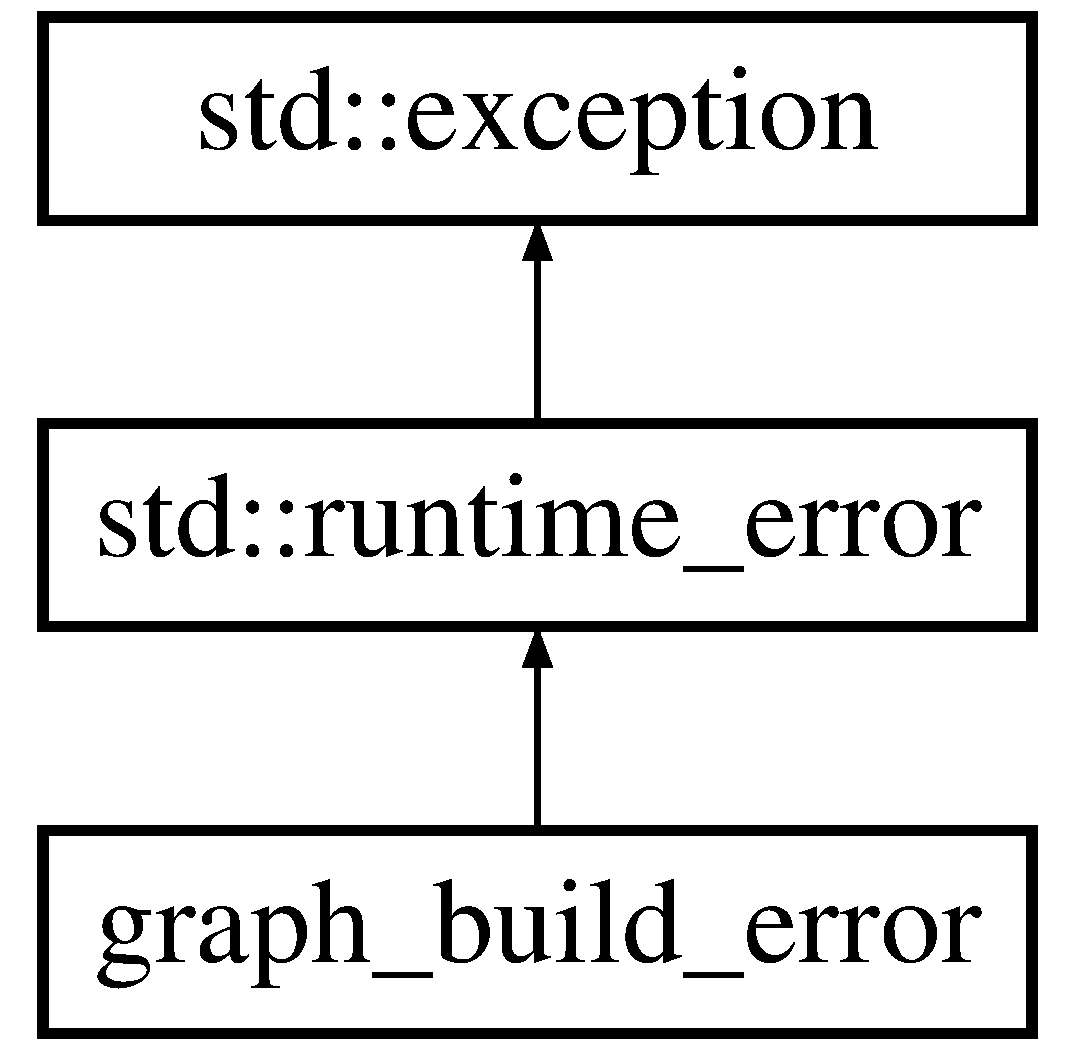
\includegraphics[height=3.000000cm]{structgraph__build__error}
\end{center}
\end{figure}
\subsection*{Public Member Functions}
\begin{DoxyCompactItemize}
\item 
\hypertarget{structgraph__build__error_a5b6da9f94efcd703d99c2617381749c1}{{\bfseries graph\+\_\+build\+\_\+error} (const string \&msg)}\label{structgraph__build__error_a5b6da9f94efcd703d99c2617381749c1}

\end{DoxyCompactItemize}


\subsection{Detailed Description}
Write what the function does here. 

\begin{DoxyReturn}{Returns}

\end{DoxyReturn}


Definition at line 24 of file graph.\+h.



The documentation for this struct was generated from the following file\+:\begin{DoxyCompactItemize}
\item 
graph.\+h\end{DoxyCompactItemize}

\hypertarget{classGUICanvas}{\section{G\+U\+I\+Canvas Class Reference}
\label{classGUICanvas}\index{G\+U\+I\+Canvas@{G\+U\+I\+Canvas}}
}


Write what the function does here.  




{\ttfamily \#include $<$guicanvas.\+h$>$}

Inheritance diagram for G\+U\+I\+Canvas\+:\begin{figure}[H]
\begin{center}
\leavevmode
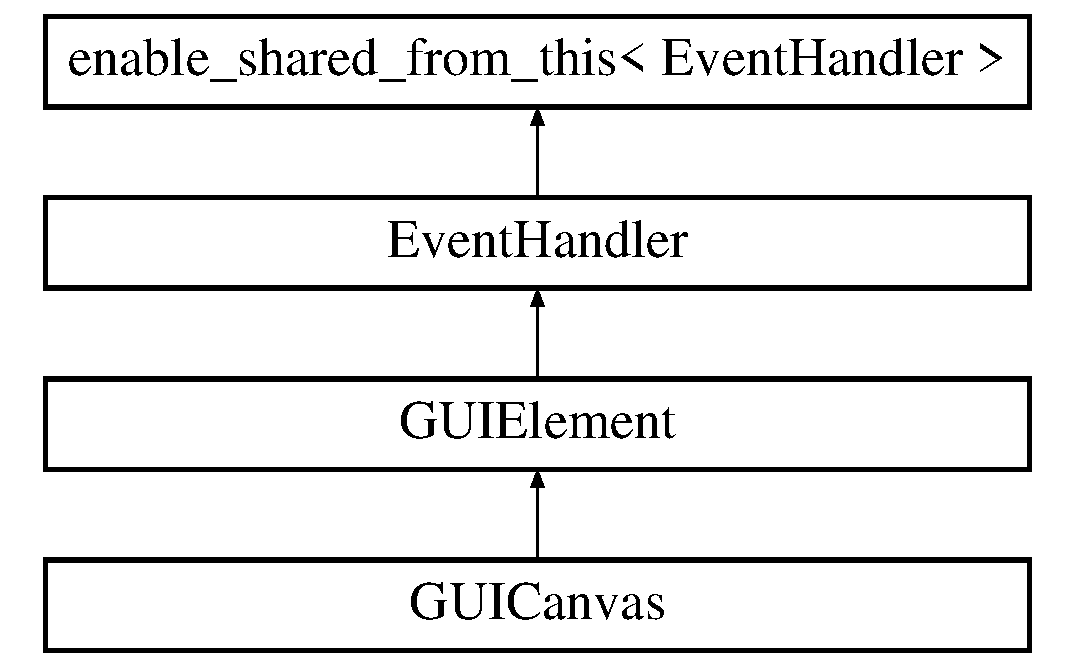
\includegraphics[height=4.000000cm]{classGUICanvas}
\end{center}
\end{figure}
\subsection*{Public Member Functions}
\begin{DoxyCompactItemize}
\item 
\hypertarget{classGUICanvas_a2e6418e2376d80fddab7a747dd15da36}{{\bfseries G\+U\+I\+Canvas} (float min\+X, float max\+X, float min\+Y, float max\+Y, function$<$ Mesh()$>$ generate\+Mesh\+Fn)}\label{classGUICanvas_a2e6418e2376d80fddab7a747dd15da36}

\end{DoxyCompactItemize}
\subsection*{Private Attributes}
\begin{DoxyCompactItemize}
\item 
\hypertarget{classGUICanvas_a3758be22090e23d9c7d566a5a08041d5}{function$<$ Mesh()$>$ {\bfseries generate\+Mesh\+Fn}}\label{classGUICanvas_a3758be22090e23d9c7d566a5a08041d5}

\end{DoxyCompactItemize}


\subsection{Detailed Description}
Write what the function does here. 


\begin{DoxyRetVals}{Return values}
{\em (variable)} & (description of variable) \\
\hline
\end{DoxyRetVals}


Definition at line 14 of file guicanvas.\+h.



The documentation for this class was generated from the following file\+:\begin{DoxyCompactItemize}
\item 
guicanvas.\+h\end{DoxyCompactItemize}

\hypertarget{classGUIContainer}{\section{G\+U\+I\+Container Class Reference}
\label{classGUIContainer}\index{G\+U\+I\+Container@{G\+U\+I\+Container}}
}


Write what the function does here.  




{\ttfamily \#include $<$guicontainer.\+h$>$}

Inheritance diagram for G\+U\+I\+Container\+:\begin{figure}[H]
\begin{center}
\leavevmode
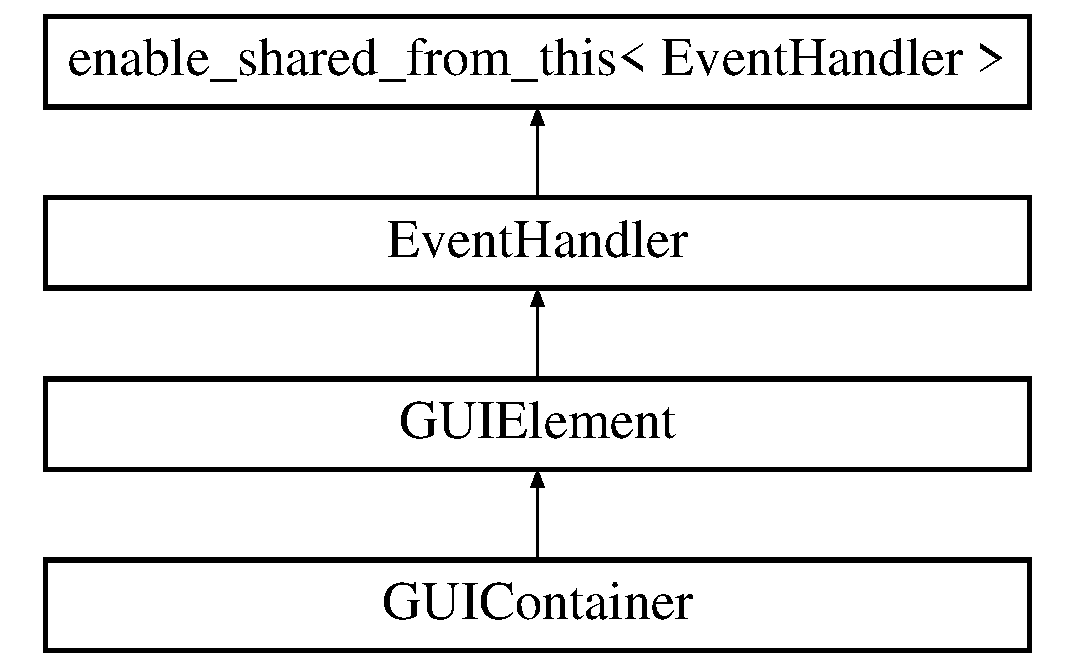
\includegraphics[height=4.000000cm]{classGUIContainer}
\end{center}
\end{figure}
\subsection*{Public Member Functions}
\begin{DoxyCompactItemize}
\item 
\hypertarget{classGUIContainer_aa35797f8b9c6a8e332ad5930faa69c00}{{\bfseries G\+U\+I\+Container} (float min\+X, float max\+X, float min\+Y, float max\+Y)}\label{classGUIContainer_aa35797f8b9c6a8e332ad5930faa69c00}

\item 
shared\+\_\+ptr$<$ \hyperlink{classGUIContainer}{G\+U\+I\+Container} $>$ \hyperlink{classGUIContainer_a01f2cf647a23b37ed7d815a9780ef8f9}{add} (shared\+\_\+ptr$<$ \hyperlink{classGUIElement}{G\+U\+I\+Element} $>$ element)
\begin{DoxyCompactList}\small\item\em Write what the function does here. \end{DoxyCompactList}\item 
virtual shared\+\_\+ptr$<$ \hyperlink{classGUIElement}{G\+U\+I\+Element} $>$ \hyperlink{classGUIContainer_addf987ba650075a7c0f34c571debd6a2}{get\+Focus\+Element} () overridefinal
\begin{DoxyCompactList}\small\item\em Write what the function does here. \end{DoxyCompactList}\item 
virtual bool \hyperlink{classGUIContainer_a54bbf86cc92ce6518ccdc25a21b8e5f5}{can\+Have\+Keyboard\+Focus} () const overridefinal
\begin{DoxyCompactList}\small\item\em Write what the function does here. \end{DoxyCompactList}\item 
virtual bool \hyperlink{classGUIContainer_afa186df2611c4e309094e8da2654f5b2}{prev\+Focus\+Element} () overridefinal
\begin{DoxyCompactList}\small\item\em Write what the function does here. \end{DoxyCompactList}\item 
virtual bool \hyperlink{classGUIContainer_a83c20737ae89ecdb0da054cec1ca087e}{next\+Focus\+Element} () overridefinal
\begin{DoxyCompactList}\small\item\em Write what the function does here. \end{DoxyCompactList}\item 
virtual bool \hyperlink{classGUIContainer_acba4796c4bec859c70f04a4f4471b3fe}{handle\+Mouse\+Up} (\hyperlink{structMouseUpEvent}{Mouse\+Up\+Event} \&\hyperlink{unionSDL__Event}{event}) overridefinal
\begin{DoxyCompactList}\small\item\em Write what the function does here. \end{DoxyCompactList}\item 
virtual bool \hyperlink{classGUIContainer_a10229d26c8bdac0e8b1c3b0e2863331a}{handle\+Mouse\+Down} (\hyperlink{structMouseDownEvent}{Mouse\+Down\+Event} \&\hyperlink{unionSDL__Event}{event}) overridefinal
\begin{DoxyCompactList}\small\item\em Write what the function does here. \end{DoxyCompactList}\item 
virtual bool \hyperlink{classGUIContainer_a9ee4ac638a114d858ab8836fb3dde441}{handle\+Mouse\+Move} (\hyperlink{structMouseMoveEvent}{Mouse\+Move\+Event} \&\hyperlink{unionSDL__Event}{event}) overridefinal
\begin{DoxyCompactList}\small\item\em Write what the function does here. \end{DoxyCompactList}\item 
virtual bool \hyperlink{classGUIContainer_a85ef65ef4de74236bb2b5f200636fa0c}{handle\+Mouse\+Move\+Out} (\hyperlink{classMouseEvent}{Mouse\+Event} \&\hyperlink{unionSDL__Event}{event}) overridefinal
\begin{DoxyCompactList}\small\item\em Write what the function does here. \end{DoxyCompactList}\item 
virtual bool \hyperlink{classGUIContainer_a5de801e62c8d14d559e3dfae68cca72d}{handle\+Mouse\+Move\+In} (\hyperlink{classMouseEvent}{Mouse\+Event} \&\hyperlink{unionSDL__Event}{event}) overridefinal
\begin{DoxyCompactList}\small\item\em Write what the function does here. \end{DoxyCompactList}\item 
virtual bool \hyperlink{classGUIContainer_a80a3c99fbdec76ac9a333a6737e9ff5a}{handle\+Mouse\+Scroll} (\hyperlink{structMouseScrollEvent}{Mouse\+Scroll\+Event} \&\hyperlink{unionSDL__Event}{event}) overridefinal
\begin{DoxyCompactList}\small\item\em Write what the function does here. \end{DoxyCompactList}\item 
virtual bool \hyperlink{classGUIContainer_a6e1ad46740bab18d77efb8f88c3a70bb}{handle\+Key\+Up} (\hyperlink{classKeyUpEvent}{Key\+Up\+Event} \&\hyperlink{unionSDL__Event}{event}) overridefinal
\begin{DoxyCompactList}\small\item\em Write what the function does here. \end{DoxyCompactList}\item 
virtual bool \hyperlink{classGUIContainer_a8dec7de665719cb1e440a655fac6b69a}{handle\+Key\+Down} (\hyperlink{classKeyDownEvent}{Key\+Down\+Event} \&\hyperlink{unionSDL__Event}{event}) overridefinal
\begin{DoxyCompactList}\small\item\em Write what the function does here. \end{DoxyCompactList}\item 
virtual bool \hyperlink{classGUIContainer_a7109d4597eb95baa047e4de213f9428f}{handle\+Key\+Press} (\hyperlink{structKeyPressEvent}{Key\+Press\+Event} \&\hyperlink{unionSDL__Event}{event}) overridefinal
\begin{DoxyCompactList}\small\item\em Write what the function does here. \end{DoxyCompactList}\item 
virtual bool \hyperlink{classGUIContainer_a1fbd8dfea04418ce139b202961987255}{handle\+Quit} (\hyperlink{structQuitEvent}{Quit\+Event} \&\hyperlink{unionSDL__Event}{event}) overridefinal
\begin{DoxyCompactList}\small\item\em Write what the function does here. \end{DoxyCompactList}\item 
virtual Mesh \hyperlink{classGUIContainer_ac0c16fc5501929f38fd6d1b325d1c801}{render} (float min\+Z, float max\+Z, bool has\+Focus) override
\begin{DoxyCompactList}\small\item\em Write what the function does here. \end{DoxyCompactList}\item 
void \hyperlink{classGUIContainer_a231ba20b33175f315be9ea08ec00a6c4}{set\+Focus} (shared\+\_\+ptr$<$ \hyperlink{classGUIElement}{G\+U\+I\+Element} $>$ e)
\begin{DoxyCompactList}\small\item\em Write what the function does here. \end{DoxyCompactList}\item 
virtual shared\+\_\+ptr$<$ \hyperlink{classGUIContainer}{G\+U\+I\+Container} $>$ \hyperlink{classGUIContainer_a4bade45ffb4a8961ba2a3e0b406d186c}{get\+Top\+Level\+Parent} () overridefinal
\begin{DoxyCompactList}\small\item\em Write what the function does here. \end{DoxyCompactList}\end{DoxyCompactItemize}
\subsection*{Protected Member Functions}
\begin{DoxyCompactItemize}
\item 
shared\+\_\+ptr$<$ \hyperlink{classGUIElement}{G\+U\+I\+Element} $>$ \hyperlink{classGUIContainer_aa284afbbc302222ac9bff04fba9bfe4e}{get\+Element} (size\+\_\+t index)
\begin{DoxyCompactList}\small\item\em Write what the function does here. \end{DoxyCompactList}\item 
size\+\_\+t \hyperlink{classGUIContainer_a65c0f2e73c3f02ea936cb37447dba04b}{get\+Element\+Count} ()
\begin{DoxyCompactList}\small\item\em Write what the function does here. \end{DoxyCompactList}\item 
size\+\_\+t \hyperlink{classGUIContainer_a2e29a0e330951f3dd35b7b81c39b5a65}{get\+Current\+Element\+Index} ()
\begin{DoxyCompactList}\small\item\em Write what the function does here. \end{DoxyCompactList}\end{DoxyCompactItemize}
\subsection*{Static Protected Attributes}
\begin{DoxyCompactItemize}
\item 
\hypertarget{classGUIContainer_a530b15ff8ab84f7a4357b5714da3c16b}{static constexpr const size\+\_\+t {\bfseries No\+Element} = (size\+\_\+t)-\/1}\label{classGUIContainer_a530b15ff8ab84f7a4357b5714da3c16b}

\end{DoxyCompactItemize}
\subsection*{Private Member Functions}
\begin{DoxyCompactItemize}
\item 
size\+\_\+t \hyperlink{classGUIContainer_a99d8776d71b5452a138842d3d2822348}{get\+Index\+From\+Position} (float x, float y)
\begin{DoxyCompactList}\small\item\em Write what the function does here. \end{DoxyCompactList}\end{DoxyCompactItemize}
\subsection*{Private Attributes}
\begin{DoxyCompactItemize}
\item 
\hypertarget{classGUIContainer_a68726b5ba87fd7a250c95df7df745f08}{vector$<$ shared\+\_\+ptr$<$ \hyperlink{classGUIElement}{G\+U\+I\+Element} $>$ $>$ {\bfseries elements}}\label{classGUIContainer_a68726b5ba87fd7a250c95df7df745f08}

\item 
\hypertarget{classGUIContainer_a88f758f83baa2b612d1a7fbed504a80e}{size\+\_\+t {\bfseries current\+Focus\+Index} = 0}\label{classGUIContainer_a88f758f83baa2b612d1a7fbed504a80e}

\item 
\hypertarget{classGUIContainer_a9270df928601ad530d7d18249bae3fd3}{size\+\_\+t {\bfseries last\+Mouse\+Element} = No\+Element}\label{classGUIContainer_a9270df928601ad530d7d18249bae3fd3}

\end{DoxyCompactItemize}


\subsection{Detailed Description}
Write what the function does here. 

\begin{DoxyReturn}{Returns}

\end{DoxyReturn}


Definition at line 12 of file guicontainer.\+h.



\subsection{Member Function Documentation}
\hypertarget{classGUIContainer_a01f2cf647a23b37ed7d815a9780ef8f9}{\index{G\+U\+I\+Container@{G\+U\+I\+Container}!add@{add}}
\index{add@{add}!G\+U\+I\+Container@{G\+U\+I\+Container}}
\subsubsection[{add}]{\setlength{\rightskip}{0pt plus 5cm}shared\+\_\+ptr$<${\bf G\+U\+I\+Container}$>$ G\+U\+I\+Container\+::add (
\begin{DoxyParamCaption}
\item[{shared\+\_\+ptr$<$ {\bf G\+U\+I\+Element} $>$}]{element}
\end{DoxyParamCaption}
)\hspace{0.3cm}{\ttfamily [inline]}}}\label{classGUIContainer_a01f2cf647a23b37ed7d815a9780ef8f9}


Write what the function does here. 


\begin{DoxyParams}{Parameters}
{\em element} & \\
\hline
\end{DoxyParams}
\begin{DoxyReturn}{Returns}

\end{DoxyReturn}


Definition at line 73 of file guicontainer.\+h.


\begin{DoxyCode}
74         \{
75             assert(element != \textcolor{keyword}{nullptr});
76             elements.push\_back(element);
77             element->parent = dynamic\_pointer\_cast<\hyperlink{classGUIContainer}{GUIContainer}>(
      \hyperlink{classGUIElement_a5ad5998c5b953b6c6e32b583ddf9cd97}{shared\_from\_this}());
78             \textcolor{keywordflow}{return} dynamic\_pointer\_cast<\hyperlink{classGUIContainer}{GUIContainer}>(
      \hyperlink{classGUIElement_a5ad5998c5b953b6c6e32b583ddf9cd97}{shared\_from\_this}());
79         \}
\end{DoxyCode}
\hypertarget{classGUIContainer_a54bbf86cc92ce6518ccdc25a21b8e5f5}{\index{G\+U\+I\+Container@{G\+U\+I\+Container}!can\+Have\+Keyboard\+Focus@{can\+Have\+Keyboard\+Focus}}
\index{can\+Have\+Keyboard\+Focus@{can\+Have\+Keyboard\+Focus}!G\+U\+I\+Container@{G\+U\+I\+Container}}
\subsubsection[{can\+Have\+Keyboard\+Focus}]{\setlength{\rightskip}{0pt plus 5cm}virtual bool G\+U\+I\+Container\+::can\+Have\+Keyboard\+Focus (
\begin{DoxyParamCaption}
{}
\end{DoxyParamCaption}
) const\hspace{0.3cm}{\ttfamily [inline]}, {\ttfamily [final]}, {\ttfamily [override]}, {\ttfamily [virtual]}}}\label{classGUIContainer_a54bbf86cc92ce6518ccdc25a21b8e5f5}


Write what the function does here. 

\begin{DoxyReturn}{Returns}

\end{DoxyReturn}


Reimplemented from \hyperlink{classGUIElement_a073ef8863e95e55df4b701f249ba4c44}{G\+U\+I\+Element}.



Definition at line 98 of file guicontainer.\+h.


\begin{DoxyCode}
99         \{
100             \textcolor{keywordflow}{for}(shared\_ptr<GUIElement> e : elements)
101                 \textcolor{keywordflow}{if}(e->canHaveKeyboardFocus())
102                     \textcolor{keywordflow}{return} \textcolor{keyword}{true};
103             \textcolor{keywordflow}{return} \textcolor{keyword}{false};
104         \}
\end{DoxyCode}
\hypertarget{classGUIContainer_a2e29a0e330951f3dd35b7b81c39b5a65}{\index{G\+U\+I\+Container@{G\+U\+I\+Container}!get\+Current\+Element\+Index@{get\+Current\+Element\+Index}}
\index{get\+Current\+Element\+Index@{get\+Current\+Element\+Index}!G\+U\+I\+Container@{G\+U\+I\+Container}}
\subsubsection[{get\+Current\+Element\+Index}]{\setlength{\rightskip}{0pt plus 5cm}size\+\_\+t G\+U\+I\+Container\+::get\+Current\+Element\+Index (
\begin{DoxyParamCaption}
{}
\end{DoxyParamCaption}
)\hspace{0.3cm}{\ttfamily [inline]}, {\ttfamily [protected]}}}\label{classGUIContainer_a2e29a0e330951f3dd35b7b81c39b5a65}


Write what the function does here. 

\begin{DoxyReturn}{Returns}

\end{DoxyReturn}


Definition at line 55 of file guicontainer.\+h.


\begin{DoxyCode}
56         \{
57             \textcolor{keywordflow}{return} currentFocusIndex;
58         \}
\end{DoxyCode}
\hypertarget{classGUIContainer_aa284afbbc302222ac9bff04fba9bfe4e}{\index{G\+U\+I\+Container@{G\+U\+I\+Container}!get\+Element@{get\+Element}}
\index{get\+Element@{get\+Element}!G\+U\+I\+Container@{G\+U\+I\+Container}}
\subsubsection[{get\+Element}]{\setlength{\rightskip}{0pt plus 5cm}shared\+\_\+ptr$<${\bf G\+U\+I\+Element}$>$ G\+U\+I\+Container\+::get\+Element (
\begin{DoxyParamCaption}
\item[{size\+\_\+t}]{index}
\end{DoxyParamCaption}
)\hspace{0.3cm}{\ttfamily [inline]}, {\ttfamily [protected]}}}\label{classGUIContainer_aa284afbbc302222ac9bff04fba9bfe4e}


Write what the function does here. 

virtual void on\+Set\+Focus() \{ \}

/$\ast$$\ast$ Write what the function does here


\begin{DoxyParams}{Parameters}
{\em index} & \\
\hline
\end{DoxyParams}
\begin{DoxyReturn}{Returns}

\end{DoxyReturn}


Definition at line 35 of file guicontainer.\+h.


\begin{DoxyCode}
36         \{
37             \textcolor{keywordflow}{return} elements[index];
38         \}
\end{DoxyCode}
\hypertarget{classGUIContainer_a65c0f2e73c3f02ea936cb37447dba04b}{\index{G\+U\+I\+Container@{G\+U\+I\+Container}!get\+Element\+Count@{get\+Element\+Count}}
\index{get\+Element\+Count@{get\+Element\+Count}!G\+U\+I\+Container@{G\+U\+I\+Container}}
\subsubsection[{get\+Element\+Count}]{\setlength{\rightskip}{0pt plus 5cm}size\+\_\+t G\+U\+I\+Container\+::get\+Element\+Count (
\begin{DoxyParamCaption}
{}
\end{DoxyParamCaption}
)\hspace{0.3cm}{\ttfamily [inline]}, {\ttfamily [protected]}}}\label{classGUIContainer_a65c0f2e73c3f02ea936cb37447dba04b}


Write what the function does here. 

\begin{DoxyReturn}{Returns}

\end{DoxyReturn}


Definition at line 45 of file guicontainer.\+h.


\begin{DoxyCode}
46         \{
47             \textcolor{keywordflow}{return} elements.size();
48         \}
\end{DoxyCode}
\hypertarget{classGUIContainer_addf987ba650075a7c0f34c571debd6a2}{\index{G\+U\+I\+Container@{G\+U\+I\+Container}!get\+Focus\+Element@{get\+Focus\+Element}}
\index{get\+Focus\+Element@{get\+Focus\+Element}!G\+U\+I\+Container@{G\+U\+I\+Container}}
\subsubsection[{get\+Focus\+Element}]{\setlength{\rightskip}{0pt plus 5cm}virtual shared\+\_\+ptr$<${\bf G\+U\+I\+Element}$>$ G\+U\+I\+Container\+::get\+Focus\+Element (
\begin{DoxyParamCaption}
{}
\end{DoxyParamCaption}
)\hspace{0.3cm}{\ttfamily [inline]}, {\ttfamily [final]}, {\ttfamily [override]}, {\ttfamily [virtual]}}}\label{classGUIContainer_addf987ba650075a7c0f34c571debd6a2}


Write what the function does here. 

\begin{DoxyReturn}{Returns}

\end{DoxyReturn}


Reimplemented from \hyperlink{classGUIElement_acdb491fec728f3a39318850fa144c766}{G\+U\+I\+Element}.



Definition at line 86 of file guicontainer.\+h.


\begin{DoxyCode}
87         \{
88             \textcolor{keywordflow}{if}(currentFocusIndex >= elements.size())
89                 \textcolor{keywordflow}{return} \hyperlink{classGUIElement_a5ad5998c5b953b6c6e32b583ddf9cd97}{shared\_from\_this}();
90             \textcolor{keywordflow}{return} elements[currentFocusIndex];
91         \}
\end{DoxyCode}
\hypertarget{classGUIContainer_a99d8776d71b5452a138842d3d2822348}{\index{G\+U\+I\+Container@{G\+U\+I\+Container}!get\+Index\+From\+Position@{get\+Index\+From\+Position}}
\index{get\+Index\+From\+Position@{get\+Index\+From\+Position}!G\+U\+I\+Container@{G\+U\+I\+Container}}
\subsubsection[{get\+Index\+From\+Position}]{\setlength{\rightskip}{0pt plus 5cm}size\+\_\+t G\+U\+I\+Container\+::get\+Index\+From\+Position (
\begin{DoxyParamCaption}
\item[{float}]{x, }
\item[{float}]{y}
\end{DoxyParamCaption}
)\hspace{0.3cm}{\ttfamily [inline]}, {\ttfamily [private]}}}\label{classGUIContainer_a99d8776d71b5452a138842d3d2822348}


Write what the function does here. 


\begin{DoxyParams}{Parameters}
{\em x} & \\
\hline
{\em y} & \\
\hline
\end{DoxyParams}
\begin{DoxyReturn}{Returns}

\end{DoxyReturn}


Definition at line 236 of file guicontainer.\+h.


\begin{DoxyCode}
237         \{
238             \hyperlink{structVectorF}{VectorF} v = Display::transformMouseTo3D(x, y);
239 
240             \textcolor{keywordflow}{for}(\textcolor{keywordtype}{size\_t} i = 0, retval = elements.size() - 1; i < elements.size(); i++, retval--)
241             \{
242                 \textcolor{keywordflow}{if}(elements[retval]->\hyperlink{classGUIElement_a5f0fe42b4b9fc20f01397e7face80ae6}{isPointInside}(v.x, v.y))
243                     \textcolor{keywordflow}{return} retval;
244             \}
245             \textcolor{keywordflow}{return} NoElement;
246         \}
\end{DoxyCode}
\hypertarget{classGUIContainer_a4bade45ffb4a8961ba2a3e0b406d186c}{\index{G\+U\+I\+Container@{G\+U\+I\+Container}!get\+Top\+Level\+Parent@{get\+Top\+Level\+Parent}}
\index{get\+Top\+Level\+Parent@{get\+Top\+Level\+Parent}!G\+U\+I\+Container@{G\+U\+I\+Container}}
\subsubsection[{get\+Top\+Level\+Parent}]{\setlength{\rightskip}{0pt plus 5cm}virtual shared\+\_\+ptr$<${\bf G\+U\+I\+Container}$>$ G\+U\+I\+Container\+::get\+Top\+Level\+Parent (
\begin{DoxyParamCaption}
{}
\end{DoxyParamCaption}
)\hspace{0.3cm}{\ttfamily [inline]}, {\ttfamily [final]}, {\ttfamily [override]}, {\ttfamily [virtual]}}}\label{classGUIContainer_a4bade45ffb4a8961ba2a3e0b406d186c}


Write what the function does here. 

virtual void reset() override \{

if(\hyperlink{classGUIElement_aded5837705c097a7a8a755df28c572e6}{get\+Parent()} == nullptr) \{ min\+X = -\/\+Display\+::scale\+X(); max\+X = Display\+::scale\+X(); min\+Y = -\/\+Display\+::scale\+Y(); max\+Y = Display\+::scale\+Y(); \} for(shared\+\_\+ptr$<$\+G\+U\+I\+Element$>$ e \+: elements) e-\/$>$reset(); first\+Focus\+Element(); \}

/$\ast$$\ast$ Write what the function does here

\begin{DoxyReturn}{Returns}

\end{DoxyReturn}


Reimplemented from \hyperlink{classGUIElement_a09eebb7ff9e98191caf3a0421f0bad8c}{G\+U\+I\+Element}.



Definition at line 600 of file guicontainer.\+h.


\begin{DoxyCode}
601         \{
602             shared\_ptr<GUIContainer> retval = dynamic\_pointer\_cast<\hyperlink{classGUIContainer}{GUIContainer}>(
      \hyperlink{classGUIElement_a5ad5998c5b953b6c6e32b583ddf9cd97}{shared\_from\_this}());
603             \textcolor{keywordflow}{while}(retval->getParent() != \textcolor{keyword}{nullptr})
604                 retval = retval->\hyperlink{classGUIElement_aded5837705c097a7a8a755df28c572e6}{getParent}();
605             \textcolor{keywordflow}{return} retval;
606         \}
\end{DoxyCode}
\hypertarget{classGUIContainer_a8dec7de665719cb1e440a655fac6b69a}{\index{G\+U\+I\+Container@{G\+U\+I\+Container}!handle\+Key\+Down@{handle\+Key\+Down}}
\index{handle\+Key\+Down@{handle\+Key\+Down}!G\+U\+I\+Container@{G\+U\+I\+Container}}
\subsubsection[{handle\+Key\+Down}]{\setlength{\rightskip}{0pt plus 5cm}virtual bool G\+U\+I\+Container\+::handle\+Key\+Down (
\begin{DoxyParamCaption}
\item[{{\bf Key\+Down\+Event} \&}]{event}
\end{DoxyParamCaption}
)\hspace{0.3cm}{\ttfamily [inline]}, {\ttfamily [final]}, {\ttfamily [override]}, {\ttfamily [virtual]}}}\label{classGUIContainer_a8dec7de665719cb1e440a655fac6b69a}


Write what the function does here. 


\begin{DoxyParams}{Parameters}
{\em event} & \\
\hline
\end{DoxyParams}
\begin{DoxyReturn}{Returns}

\end{DoxyReturn}


Reimplemented from \hyperlink{classGUIElement_aa85f949aa746eac4deadfa0bb8827f71}{G\+U\+I\+Element}.



Definition at line 441 of file guicontainer.\+h.


\begin{DoxyCode}
442         \{
443             shared\_ptr<GUIElement> e = \hyperlink{classGUIContainer_addf987ba650075a7c0f34c571debd6a2}{getFocusElement}();
444             \textcolor{keywordtype}{bool} retval;
445             \textcolor{keywordflow}{if}(e == \hyperlink{classGUIElement_a5ad5998c5b953b6c6e32b583ddf9cd97}{shared\_from\_this}())
446                 retval = \hyperlink{classGUIElement_aa85f949aa746eac4deadfa0bb8827f71}{GUIElement::handleKeyDown}(event);
447             \textcolor{keywordflow}{else}
448                 retval = e->handleKeyDown(event);
449             \textcolor{keywordflow}{if}(retval)
450                 \textcolor{keywordflow}{return} \textcolor{keyword}{true};
451             \textcolor{keywordflow}{if}(\hyperlink{classGUIElement_aded5837705c097a7a8a755df28c572e6}{getParent}() != \textcolor{keyword}{nullptr} || (event.mods & (KeyboardModifiers\_Ctrl | 
      KeyboardModifiers\_Alt | KeyboardModifiers\_Meta | KeyboardModifiers\_Mode)) != 0)
452                 \textcolor{keywordflow}{return} \textcolor{keyword}{false};
453 
454             \textcolor{keywordflow}{if}(event.key == KeyboardKey\_Tab)
455             \{
456                 \textcolor{keywordflow}{if}(event.mods & KeyboardModifiers\_Shift)
457                     \hyperlink{classGUIContainer_afa186df2611c4e309094e8da2654f5b2}{prevFocusElement}();
458                 \textcolor{keywordflow}{else}
459                     \hyperlink{classGUIContainer_a83c20737ae89ecdb0da054cec1ca087e}{nextFocusElement}();
460                 \textcolor{keywordflow}{return} \textcolor{keyword}{true};
461             \}
462             \textcolor{keywordflow}{else} \textcolor{keywordflow}{if}(event.mods & KeyboardModifiers\_Shift)
463                 \textcolor{keywordflow}{return} \textcolor{keyword}{false};
464 
465             \textcolor{keywordflow}{else} \textcolor{keywordflow}{if}(event.key == KeyboardKey\_Down)
466             \{
467                 \hyperlink{classGUIContainer_a83c20737ae89ecdb0da054cec1ca087e}{nextFocusElement}();
468                 \textcolor{keywordflow}{return} \textcolor{keyword}{true};
469             \}
470 
471             \textcolor{keywordflow}{else} \textcolor{keywordflow}{if}(event.key == KeyboardKey\_Up)
472             \{
473                 \hyperlink{classGUIContainer_afa186df2611c4e309094e8da2654f5b2}{prevFocusElement}();
474                 \textcolor{keywordflow}{return} \textcolor{keyword}{true};
475             \}
476 
477             \textcolor{keywordflow}{else} \textcolor{keywordflow}{if}(event.key == KeyboardKey\_Home)
478             \{
479                 firstFocusElement();
480                 \textcolor{keywordflow}{return} \textcolor{keyword}{true};
481             \}
482 
483             \textcolor{keywordflow}{else} \textcolor{keywordflow}{if}(event.key == KeyboardKey\_End)
484             \{
485                 lastFocusElement();
486                 \textcolor{keywordflow}{return} \textcolor{keyword}{true};
487             \}
488             \textcolor{keywordflow}{return} \textcolor{keyword}{false};
489         \}
\end{DoxyCode}
\hypertarget{classGUIContainer_a7109d4597eb95baa047e4de213f9428f}{\index{G\+U\+I\+Container@{G\+U\+I\+Container}!handle\+Key\+Press@{handle\+Key\+Press}}
\index{handle\+Key\+Press@{handle\+Key\+Press}!G\+U\+I\+Container@{G\+U\+I\+Container}}
\subsubsection[{handle\+Key\+Press}]{\setlength{\rightskip}{0pt plus 5cm}virtual bool G\+U\+I\+Container\+::handle\+Key\+Press (
\begin{DoxyParamCaption}
\item[{{\bf Key\+Press\+Event} \&}]{event}
\end{DoxyParamCaption}
)\hspace{0.3cm}{\ttfamily [inline]}, {\ttfamily [final]}, {\ttfamily [override]}, {\ttfamily [virtual]}}}\label{classGUIContainer_a7109d4597eb95baa047e4de213f9428f}


Write what the function does here. 


\begin{DoxyParams}{Parameters}
{\em event} & \\
\hline
\end{DoxyParams}
\begin{DoxyReturn}{Returns}

\end{DoxyReturn}


Reimplemented from \hyperlink{classGUIElement_ac5b578dfd0da486e32d4cf223b2d6513}{G\+U\+I\+Element}.



Definition at line 498 of file guicontainer.\+h.


\begin{DoxyCode}
499         \{
500             shared\_ptr<GUIElement> e = \hyperlink{classGUIContainer_addf987ba650075a7c0f34c571debd6a2}{getFocusElement}();
501             \textcolor{keywordflow}{if}(e == \hyperlink{classGUIElement_a5ad5998c5b953b6c6e32b583ddf9cd97}{shared\_from\_this}())
502                 \textcolor{keywordflow}{return} \hyperlink{classGUIElement_ac5b578dfd0da486e32d4cf223b2d6513}{GUIElement::handleKeyPress}(event);
503             \textcolor{keywordflow}{return} e->handleKeyPress(event);
504         \}
\end{DoxyCode}
\hypertarget{classGUIContainer_a6e1ad46740bab18d77efb8f88c3a70bb}{\index{G\+U\+I\+Container@{G\+U\+I\+Container}!handle\+Key\+Up@{handle\+Key\+Up}}
\index{handle\+Key\+Up@{handle\+Key\+Up}!G\+U\+I\+Container@{G\+U\+I\+Container}}
\subsubsection[{handle\+Key\+Up}]{\setlength{\rightskip}{0pt plus 5cm}virtual bool G\+U\+I\+Container\+::handle\+Key\+Up (
\begin{DoxyParamCaption}
\item[{{\bf Key\+Up\+Event} \&}]{event}
\end{DoxyParamCaption}
)\hspace{0.3cm}{\ttfamily [inline]}, {\ttfamily [final]}, {\ttfamily [override]}, {\ttfamily [virtual]}}}\label{classGUIContainer_a6e1ad46740bab18d77efb8f88c3a70bb}


Write what the function does here. 


\begin{DoxyParams}{Parameters}
{\em event} & \\
\hline
\end{DoxyParams}
\begin{DoxyReturn}{Returns}

\end{DoxyReturn}


Reimplemented from \hyperlink{classGUIElement_a7f0049f13cb199d09b6cf2e61ea8e7a3}{G\+U\+I\+Element}.



Definition at line 426 of file guicontainer.\+h.


\begin{DoxyCode}
427         \{
428             shared\_ptr<GUIElement> e = \hyperlink{classGUIContainer_addf987ba650075a7c0f34c571debd6a2}{getFocusElement}();
429             \textcolor{keywordflow}{if}(e == \hyperlink{classGUIElement_a5ad5998c5b953b6c6e32b583ddf9cd97}{shared\_from\_this}())
430                 \textcolor{keywordflow}{return} \hyperlink{classGUIElement_a7f0049f13cb199d09b6cf2e61ea8e7a3}{GUIElement::handleKeyUp}(event);
431             \textcolor{keywordflow}{return} e->handleKeyUp(event);
432         \}
\end{DoxyCode}
\hypertarget{classGUIContainer_a10229d26c8bdac0e8b1c3b0e2863331a}{\index{G\+U\+I\+Container@{G\+U\+I\+Container}!handle\+Mouse\+Down@{handle\+Mouse\+Down}}
\index{handle\+Mouse\+Down@{handle\+Mouse\+Down}!G\+U\+I\+Container@{G\+U\+I\+Container}}
\subsubsection[{handle\+Mouse\+Down}]{\setlength{\rightskip}{0pt plus 5cm}virtual bool G\+U\+I\+Container\+::handle\+Mouse\+Down (
\begin{DoxyParamCaption}
\item[{{\bf Mouse\+Down\+Event} \&}]{event}
\end{DoxyParamCaption}
)\hspace{0.3cm}{\ttfamily [inline]}, {\ttfamily [final]}, {\ttfamily [override]}, {\ttfamily [virtual]}}}\label{classGUIContainer_a10229d26c8bdac0e8b1c3b0e2863331a}


Write what the function does here. 


\begin{DoxyParams}{Parameters}
{\em event} & \\
\hline
\end{DoxyParams}
\begin{DoxyReturn}{Returns}

\end{DoxyReturn}


Reimplemented from \hyperlink{classGUIElement_a4809909ae2b25f816407da43b4a8f771}{G\+U\+I\+Element}.



Definition at line 289 of file guicontainer.\+h.


\begin{DoxyCode}
290         \{
291             \textcolor{keywordtype}{size\_t} index = \hyperlink{classGUIContainer_a99d8776d71b5452a138842d3d2822348}{getIndexFromPosition}(event.x, event.y);
292 
293             \textcolor{keywordflow}{if}(index != lastMouseElement)
294             \{
295 
296                 \textcolor{keywordflow}{if}(lastMouseElement != NoElement)
297                 \{
298                     elements[lastMouseElement]->handleMouseMoveOut(event);
299                 \}
300                 lastMouseElement = index;
301 
302                 \textcolor{keywordflow}{if}(index != NoElement)
303                 \{
304                     elements[index]->handleMouseMoveIn(event);
305                 \}
306             \}
307 
308             \textcolor{keywordflow}{if}(index != NoElement)
309             \{
310                 \textcolor{keywordflow}{return} elements[index]->handleMouseDown(event);
311             \}
312             \textcolor{keywordflow}{return} \hyperlink{classGUIElement_a4809909ae2b25f816407da43b4a8f771}{GUIElement::handleMouseDown}(event);
313         \}
\end{DoxyCode}
\hypertarget{classGUIContainer_a9ee4ac638a114d858ab8836fb3dde441}{\index{G\+U\+I\+Container@{G\+U\+I\+Container}!handle\+Mouse\+Move@{handle\+Mouse\+Move}}
\index{handle\+Mouse\+Move@{handle\+Mouse\+Move}!G\+U\+I\+Container@{G\+U\+I\+Container}}
\subsubsection[{handle\+Mouse\+Move}]{\setlength{\rightskip}{0pt plus 5cm}virtual bool G\+U\+I\+Container\+::handle\+Mouse\+Move (
\begin{DoxyParamCaption}
\item[{{\bf Mouse\+Move\+Event} \&}]{event}
\end{DoxyParamCaption}
)\hspace{0.3cm}{\ttfamily [inline]}, {\ttfamily [final]}, {\ttfamily [override]}, {\ttfamily [virtual]}}}\label{classGUIContainer_a9ee4ac638a114d858ab8836fb3dde441}


Write what the function does here. 


\begin{DoxyParams}{Parameters}
{\em event} & \\
\hline
\end{DoxyParams}
\begin{DoxyReturn}{Returns}

\end{DoxyReturn}


Reimplemented from \hyperlink{classGUIElement_a82b0ee7067d1c1deaef595f312592c5a}{G\+U\+I\+Element}.



Definition at line 322 of file guicontainer.\+h.


\begin{DoxyCode}
323         \{
324             \textcolor{keywordtype}{size\_t} index = \hyperlink{classGUIContainer_a99d8776d71b5452a138842d3d2822348}{getIndexFromPosition}(event.x, event.y);
325 
326             \textcolor{keywordflow}{if}(index != lastMouseElement)
327             \{
328 
329                 \textcolor{keywordflow}{if}(lastMouseElement != NoElement)
330                 \{
331                     elements[lastMouseElement]->handleMouseMoveOut(event);
332                 \}
333                 lastMouseElement = index;
334 
335                 \textcolor{keywordflow}{if}(index != NoElement)
336                 \{
337                     elements[index]->handleMouseMoveIn(event);
338                 \}
339             \}
340 
341             \textcolor{keywordflow}{if}(index != NoElement)
342             \{
343                 \textcolor{keywordflow}{return} elements[index]->handleMouseMove(event);
344             \}
345             \textcolor{keywordflow}{return} \hyperlink{classGUIElement_a82b0ee7067d1c1deaef595f312592c5a}{GUIElement::handleMouseMove}(event);
346         \}
\end{DoxyCode}
\hypertarget{classGUIContainer_a5de801e62c8d14d559e3dfae68cca72d}{\index{G\+U\+I\+Container@{G\+U\+I\+Container}!handle\+Mouse\+Move\+In@{handle\+Mouse\+Move\+In}}
\index{handle\+Mouse\+Move\+In@{handle\+Mouse\+Move\+In}!G\+U\+I\+Container@{G\+U\+I\+Container}}
\subsubsection[{handle\+Mouse\+Move\+In}]{\setlength{\rightskip}{0pt plus 5cm}virtual bool G\+U\+I\+Container\+::handle\+Mouse\+Move\+In (
\begin{DoxyParamCaption}
\item[{{\bf Mouse\+Event} \&}]{event}
\end{DoxyParamCaption}
)\hspace{0.3cm}{\ttfamily [inline]}, {\ttfamily [final]}, {\ttfamily [override]}, {\ttfamily [virtual]}}}\label{classGUIContainer_a5de801e62c8d14d559e3dfae68cca72d}


Write what the function does here. 


\begin{DoxyParams}{Parameters}
{\em event} & \\
\hline
\end{DoxyParams}
\begin{DoxyReturn}{Returns}

\end{DoxyReturn}


Reimplemented from \hyperlink{classGUIElement_ae1c939c5af3544b9a5967b9035623459}{G\+U\+I\+Element}.



Definition at line 374 of file guicontainer.\+h.


\begin{DoxyCode}
375         \{
376             \textcolor{keywordtype}{size\_t} index = \hyperlink{classGUIContainer_a99d8776d71b5452a138842d3d2822348}{getIndexFromPosition}(event.x, event.y);
377             lastMouseElement = index;
378 
379             \textcolor{keywordflow}{if}(index != NoElement)
380             \{
381                 \textcolor{keywordflow}{return} elements[index]->handleMouseMoveIn(event);
382             \}
383             \textcolor{keywordflow}{return} \hyperlink{classGUIElement_ae1c939c5af3544b9a5967b9035623459}{GUIElement::handleMouseMoveIn}(event);
384         \}
\end{DoxyCode}
\hypertarget{classGUIContainer_a85ef65ef4de74236bb2b5f200636fa0c}{\index{G\+U\+I\+Container@{G\+U\+I\+Container}!handle\+Mouse\+Move\+Out@{handle\+Mouse\+Move\+Out}}
\index{handle\+Mouse\+Move\+Out@{handle\+Mouse\+Move\+Out}!G\+U\+I\+Container@{G\+U\+I\+Container}}
\subsubsection[{handle\+Mouse\+Move\+Out}]{\setlength{\rightskip}{0pt plus 5cm}virtual bool G\+U\+I\+Container\+::handle\+Mouse\+Move\+Out (
\begin{DoxyParamCaption}
\item[{{\bf Mouse\+Event} \&}]{event}
\end{DoxyParamCaption}
)\hspace{0.3cm}{\ttfamily [inline]}, {\ttfamily [final]}, {\ttfamily [override]}, {\ttfamily [virtual]}}}\label{classGUIContainer_a85ef65ef4de74236bb2b5f200636fa0c}


Write what the function does here. 


\begin{DoxyParams}{Parameters}
{\em event} & \\
\hline
\end{DoxyParams}
\begin{DoxyReturn}{Returns}

\end{DoxyReturn}


Reimplemented from \hyperlink{classGUIElement_a0e4fe2486bff60c1dfcd058244be7acf}{G\+U\+I\+Element}.



Definition at line 355 of file guicontainer.\+h.


\begin{DoxyCode}
356         \{
357 
358             \textcolor{keywordflow}{if}(lastMouseElement != NoElement)
359             \{
360                 shared\_ptr<GUIElement> e = elements[lastMouseElement];
361                 lastMouseElement = NoElement;
362                 \textcolor{keywordflow}{return} e->handleMouseMoveOut(event);
363             \}
364             \textcolor{keywordflow}{return} \hyperlink{classGUIElement_a0e4fe2486bff60c1dfcd058244be7acf}{GUIElement::handleMouseMoveOut}(event);
365         \}
\end{DoxyCode}
\hypertarget{classGUIContainer_a80a3c99fbdec76ac9a333a6737e9ff5a}{\index{G\+U\+I\+Container@{G\+U\+I\+Container}!handle\+Mouse\+Scroll@{handle\+Mouse\+Scroll}}
\index{handle\+Mouse\+Scroll@{handle\+Mouse\+Scroll}!G\+U\+I\+Container@{G\+U\+I\+Container}}
\subsubsection[{handle\+Mouse\+Scroll}]{\setlength{\rightskip}{0pt plus 5cm}virtual bool G\+U\+I\+Container\+::handle\+Mouse\+Scroll (
\begin{DoxyParamCaption}
\item[{{\bf Mouse\+Scroll\+Event} \&}]{event}
\end{DoxyParamCaption}
)\hspace{0.3cm}{\ttfamily [inline]}, {\ttfamily [final]}, {\ttfamily [override]}, {\ttfamily [virtual]}}}\label{classGUIContainer_a80a3c99fbdec76ac9a333a6737e9ff5a}


Write what the function does here. 


\begin{DoxyParams}{Parameters}
{\em event} & \\
\hline
\end{DoxyParams}
\begin{DoxyReturn}{Returns}

\end{DoxyReturn}


Reimplemented from \hyperlink{classGUIElement_a3640473a7fb9651a1298122a0e0a8b29}{G\+U\+I\+Element}.



Definition at line 393 of file guicontainer.\+h.


\begin{DoxyCode}
394         \{
395             \textcolor{keywordtype}{size\_t} index = \hyperlink{classGUIContainer_a99d8776d71b5452a138842d3d2822348}{getIndexFromPosition}(event.x, event.y);
396 
397             \textcolor{keywordflow}{if}(index != lastMouseElement)
398             \{
399 
400                 \textcolor{keywordflow}{if}(lastMouseElement != NoElement)
401                 \{
402                     elements[lastMouseElement]->handleMouseMoveOut(event);
403                 \}
404                 lastMouseElement = index;
405 
406                 \textcolor{keywordflow}{if}(index != NoElement)
407                 \{
408                     elements[index]->handleMouseMoveIn(event);
409                 \}
410             \}
411 
412             \textcolor{keywordflow}{if}(index != NoElement)
413             \{
414                 \textcolor{keywordflow}{return} elements[index]->handleMouseScroll(event);
415             \}
416             \textcolor{keywordflow}{return} \hyperlink{classGUIElement_a3640473a7fb9651a1298122a0e0a8b29}{GUIElement::handleMouseScroll}(event);
417         \}
\end{DoxyCode}
\hypertarget{classGUIContainer_acba4796c4bec859c70f04a4f4471b3fe}{\index{G\+U\+I\+Container@{G\+U\+I\+Container}!handle\+Mouse\+Up@{handle\+Mouse\+Up}}
\index{handle\+Mouse\+Up@{handle\+Mouse\+Up}!G\+U\+I\+Container@{G\+U\+I\+Container}}
\subsubsection[{handle\+Mouse\+Up}]{\setlength{\rightskip}{0pt plus 5cm}virtual bool G\+U\+I\+Container\+::handle\+Mouse\+Up (
\begin{DoxyParamCaption}
\item[{{\bf Mouse\+Up\+Event} \&}]{event}
\end{DoxyParamCaption}
)\hspace{0.3cm}{\ttfamily [inline]}, {\ttfamily [final]}, {\ttfamily [override]}, {\ttfamily [virtual]}}}\label{classGUIContainer_acba4796c4bec859c70f04a4f4471b3fe}


Write what the function does here. 


\begin{DoxyParams}{Parameters}
{\em event} & \\
\hline
\end{DoxyParams}
\begin{DoxyReturn}{Returns}

\end{DoxyReturn}


Reimplemented from \hyperlink{classGUIElement_afcccb09fab792ee06ab929dec8a9d8e7}{G\+U\+I\+Element}.



Definition at line 256 of file guicontainer.\+h.


\begin{DoxyCode}
257         \{
258             \textcolor{keywordtype}{size\_t} index = \hyperlink{classGUIContainer_a99d8776d71b5452a138842d3d2822348}{getIndexFromPosition}(event.x, event.y);
259 
260             \textcolor{keywordflow}{if}(index != lastMouseElement)
261             \{
262 
263                 \textcolor{keywordflow}{if}(lastMouseElement != NoElement)
264                 \{
265                     elements[lastMouseElement]->handleMouseMoveOut(event);
266                 \}
267                 lastMouseElement = index;
268 
269                 \textcolor{keywordflow}{if}(index != NoElement)
270                 \{
271                     elements[index]->handleMouseMoveIn(event);
272                 \}
273             \}
274 
275             \textcolor{keywordflow}{if}(index != NoElement)
276             \{
277                 \textcolor{keywordflow}{return} elements[index]->handleMouseUp(event);
278             \}
279             \textcolor{keywordflow}{return} \hyperlink{classGUIElement_afcccb09fab792ee06ab929dec8a9d8e7}{GUIElement::handleMouseUp}(event);
280         \}
\end{DoxyCode}
\hypertarget{classGUIContainer_a1fbd8dfea04418ce139b202961987255}{\index{G\+U\+I\+Container@{G\+U\+I\+Container}!handle\+Quit@{handle\+Quit}}
\index{handle\+Quit@{handle\+Quit}!G\+U\+I\+Container@{G\+U\+I\+Container}}
\subsubsection[{handle\+Quit}]{\setlength{\rightskip}{0pt plus 5cm}virtual bool G\+U\+I\+Container\+::handle\+Quit (
\begin{DoxyParamCaption}
\item[{{\bf Quit\+Event} \&}]{event}
\end{DoxyParamCaption}
)\hspace{0.3cm}{\ttfamily [inline]}, {\ttfamily [final]}, {\ttfamily [override]}, {\ttfamily [virtual]}}}\label{classGUIContainer_a1fbd8dfea04418ce139b202961987255}


Write what the function does here. 


\begin{DoxyParams}{Parameters}
{\em event} & \\
\hline
\end{DoxyParams}
\begin{DoxyReturn}{Returns}

\end{DoxyReturn}


Reimplemented from \hyperlink{classGUIElement_a03dc64741eed1946966776ac3af96e65}{G\+U\+I\+Element}.



Definition at line 513 of file guicontainer.\+h.


\begin{DoxyCode}
514         \{
515             shared\_ptr<GUIElement> e = \hyperlink{classGUIContainer_addf987ba650075a7c0f34c571debd6a2}{getFocusElement}();
516             \textcolor{keywordflow}{if}(e == \hyperlink{classGUIElement_a5ad5998c5b953b6c6e32b583ddf9cd97}{shared\_from\_this}())
517                 \textcolor{keywordflow}{return} \hyperlink{classGUIElement_a03dc64741eed1946966776ac3af96e65}{GUIElement::handleQuit}(event);
518             \textcolor{keywordflow}{return} e->handleQuit(event);
519         \}
\end{DoxyCode}
\hypertarget{classGUIContainer_a83c20737ae89ecdb0da054cec1ca087e}{\index{G\+U\+I\+Container@{G\+U\+I\+Container}!next\+Focus\+Element@{next\+Focus\+Element}}
\index{next\+Focus\+Element@{next\+Focus\+Element}!G\+U\+I\+Container@{G\+U\+I\+Container}}
\subsubsection[{next\+Focus\+Element}]{\setlength{\rightskip}{0pt plus 5cm}virtual bool G\+U\+I\+Container\+::next\+Focus\+Element (
\begin{DoxyParamCaption}
{}
\end{DoxyParamCaption}
)\hspace{0.3cm}{\ttfamily [inline]}, {\ttfamily [final]}, {\ttfamily [override]}, {\ttfamily [virtual]}}}\label{classGUIContainer_a83c20737ae89ecdb0da054cec1ca087e}


Write what the function does here. 

true when reached container boundary Write what the function does here

\begin{DoxyReturn}{Returns}

\end{DoxyReturn}


Reimplemented from \hyperlink{classGUIElement_a72dffcca76f328b780c346369d7cf325}{G\+U\+I\+Element}.



Definition at line 192 of file guicontainer.\+h.


\begin{DoxyCode}
193         \{
194             \textcolor{keywordflow}{if}(elements.size() == 0)
195                 \textcolor{keywordflow}{return} \textcolor{keyword}{true};
196 
197             \textcolor{keywordflow}{if}(currentFocusIndex >= elements.size())
198             \{
199                 currentFocusIndex = 0;
200                 \textcolor{keywordflow}{return} \textcolor{keyword}{true};
201             \}
202             \textcolor{keywordflow}{if}(!elements[currentFocusIndex]->\hyperlink{classGUIContainer_a83c20737ae89ecdb0da054cec1ca087e}{nextFocusElement}())
203                 \textcolor{keywordflow}{return} \textcolor{keyword}{false};
204 \textcolor{comment}{}
205 \textcolor{comment}{            /**}
206 \textcolor{comment}{             * @brief Write what the function does here}
207 \textcolor{comment}{             *}
208 \textcolor{comment}{             * @return}
209 \textcolor{comment}{             **/}
210             \textcolor{keywordflow}{do}
211             \{
212                 currentFocusIndex++;
213                 currentFocusIndex %= elements.size();
214 
215                 \textcolor{keywordflow}{if}(elements[currentFocusIndex]->\hyperlink{classGUIContainer_a54bbf86cc92ce6518ccdc25a21b8e5f5}{canHaveKeyboardFocus}())
216                 \{
217                     elements[currentFocusIndex]->firstFocusElement();
218                     onSetFocus();
219                     \textcolor{keywordflow}{return} currentFocusIndex == 0;
220                 \}
221             \}
222             \textcolor{keywordflow}{while}(currentFocusIndex != 0);
223             firstFocusElement();
224             \textcolor{keywordflow}{return} \textcolor{keyword}{true};
225         \}
\end{DoxyCode}
\hypertarget{classGUIContainer_afa186df2611c4e309094e8da2654f5b2}{\index{G\+U\+I\+Container@{G\+U\+I\+Container}!prev\+Focus\+Element@{prev\+Focus\+Element}}
\index{prev\+Focus\+Element@{prev\+Focus\+Element}!G\+U\+I\+Container@{G\+U\+I\+Container}}
\subsubsection[{prev\+Focus\+Element}]{\setlength{\rightskip}{0pt plus 5cm}virtual bool G\+U\+I\+Container\+::prev\+Focus\+Element (
\begin{DoxyParamCaption}
{}
\end{DoxyParamCaption}
)\hspace{0.3cm}{\ttfamily [inline]}, {\ttfamily [final]}, {\ttfamily [override]}, {\ttfamily [virtual]}}}\label{classGUIContainer_afa186df2611c4e309094e8da2654f5b2}


Write what the function does here. 

virtual void first\+Focus\+Element() override final \{

for(current\+Focus\+Index = 0; current\+Focus\+Index $<$ elements.\+size(); current\+Focus\+Index++) \{

if(elements\mbox{[}current\+Focus\+Index\mbox{]}-\/$>$\hyperlink{classGUIContainer_a54bbf86cc92ce6518ccdc25a21b8e5f5}{can\+Have\+Keyboard\+Focus()}) \{ elements\mbox{[}current\+Focus\+Index\mbox{]}-\/$>$first\+Focus\+Element(); on\+Set\+Focus(); return; \} \} current\+Focus\+Index = 0; on\+Set\+Focus(); \}

/$\ast$$\ast$ Write what the function does here

virtual void last\+Focus\+Element() override final \{ current\+Focus\+Index = elements.\+size() -\/ 1;

for(size\+\_\+t i = 0; i $<$ elements.\+size(); current\+Focus\+Index--, i++) \{

if(elements\mbox{[}current\+Focus\+Index\mbox{]}-\/$>$\hyperlink{classGUIContainer_a54bbf86cc92ce6518ccdc25a21b8e5f5}{can\+Have\+Keyboard\+Focus()}) \{ elements\mbox{[}current\+Focus\+Index\mbox{]}-\/$>$last\+Focus\+Element(); on\+Set\+Focus(); return; \} \} current\+Focus\+Index = 0; on\+Set\+Focus(); \}

/$\ast$$\ast$ Write what the function does here

true when reached container boundary Write what the function does here

\begin{DoxyReturn}{Returns}

\end{DoxyReturn}


Reimplemented from \hyperlink{classGUIElement_a970e90bbb7db5de07708b0b2ef53d9e9}{G\+U\+I\+Element}.



Definition at line 152 of file guicontainer.\+h.


\begin{DoxyCode}
153         \{
154             \textcolor{keywordflow}{if}(elements.size() == 0)
155                 \textcolor{keywordflow}{return} \textcolor{keyword}{true};
156 
157             \textcolor{keywordflow}{if}(currentFocusIndex >= elements.size())
158             \{
159                 currentFocusIndex = 0;
160                 \textcolor{keywordflow}{return} \textcolor{keyword}{true};
161             \}
162             \textcolor{keywordflow}{if}(!elements[currentFocusIndex]->\hyperlink{classGUIContainer_afa186df2611c4e309094e8da2654f5b2}{prevFocusElement}())
163                 \textcolor{keywordflow}{return} \textcolor{keyword}{false};
164 \textcolor{comment}{}
165 \textcolor{comment}{            /**}
166 \textcolor{comment}{             * @brief Write what the function does here}
167 \textcolor{comment}{             *}
168 \textcolor{comment}{             * @return}
169 \textcolor{comment}{             **/}
170             \textcolor{keywordflow}{do}
171             \{
172                 currentFocusIndex += elements.size() - 1;
173                 currentFocusIndex %= elements.size();
174 
175                 \textcolor{keywordflow}{if}(elements[currentFocusIndex]->\hyperlink{classGUIContainer_a54bbf86cc92ce6518ccdc25a21b8e5f5}{canHaveKeyboardFocus}())
176                 \{
177                     elements[currentFocusIndex]->lastFocusElement();
178                     onSetFocus();
179                     \textcolor{keywordflow}{return} currentFocusIndex == elements.size() - 1;
180                 \}
181             \}
182             \textcolor{keywordflow}{while}(currentFocusIndex != elements.size() - 1);
183             lastFocusElement();
184             \textcolor{keywordflow}{return} \textcolor{keyword}{true};
185         \}
\end{DoxyCode}
\hypertarget{classGUIContainer_ac0c16fc5501929f38fd6d1b325d1c801}{\index{G\+U\+I\+Container@{G\+U\+I\+Container}!render@{render}}
\index{render@{render}!G\+U\+I\+Container@{G\+U\+I\+Container}}
\subsubsection[{render}]{\setlength{\rightskip}{0pt plus 5cm}virtual Mesh G\+U\+I\+Container\+::render (
\begin{DoxyParamCaption}
\item[{float}]{min\+Z, }
\item[{float}]{max\+Z, }
\item[{bool}]{has\+Focus}
\end{DoxyParamCaption}
)\hspace{0.3cm}{\ttfamily [inline]}, {\ttfamily [override]}, {\ttfamily [virtual]}}}\label{classGUIContainer_ac0c16fc5501929f38fd6d1b325d1c801}


Write what the function does here. 


\begin{DoxyParams}{Parameters}
{\em min\+Z} & \\
\hline
{\em max\+Z} & \\
\hline
{\em has\+Focus} & \\
\hline
\end{DoxyParams}
\begin{DoxyReturn}{Returns}

\end{DoxyReturn}


Definition at line 530 of file guicontainer.\+h.


\begin{DoxyCode}
531         \{
532             Mesh retval = \textcolor{keyword}{nullptr};
533 
534             \textcolor{keywordflow}{for}(\textcolor{keywordtype}{size\_t} i = 0; i < elements.size(); i++)
535             \{
536                 Mesh mesh = elements[i]->render(interpolate((\textcolor{keywordtype}{float})(i + 1) / elements.size(), maxZ, minZ), 
      interpolate((\textcolor{keywordtype}{float})i / elements.size(), maxZ, minZ), hasFocus && i == currentFocusIndex);
537                 \textcolor{keywordflow}{if}(retval != \textcolor{keyword}{nullptr})
538                     retval->add(mesh);
539                 \textcolor{keywordflow}{else}
540                     retval = mesh;
541             \}
542             \textcolor{keywordflow}{if}(retval == \textcolor{keyword}{nullptr})
543                 \textcolor{keywordflow}{return} Mesh(\textcolor{keyword}{new} \hyperlink{classMesh__t}{Mesh\_t}());
544             \textcolor{keywordflow}{return} retval;
545         \}
\end{DoxyCode}
\hypertarget{classGUIContainer_a231ba20b33175f315be9ea08ec00a6c4}{\index{G\+U\+I\+Container@{G\+U\+I\+Container}!set\+Focus@{set\+Focus}}
\index{set\+Focus@{set\+Focus}!G\+U\+I\+Container@{G\+U\+I\+Container}}
\subsubsection[{set\+Focus}]{\setlength{\rightskip}{0pt plus 5cm}void G\+U\+I\+Container\+::set\+Focus (
\begin{DoxyParamCaption}
\item[{shared\+\_\+ptr$<$ {\bf G\+U\+I\+Element} $>$}]{e}
\end{DoxyParamCaption}
)\hspace{0.3cm}{\ttfamily [inline]}}}\label{classGUIContainer_a231ba20b33175f315be9ea08ec00a6c4}


Write what the function does here. 


\begin{DoxyParams}{Parameters}
{\em e} & \\
\hline
\end{DoxyParams}


Definition at line 552 of file guicontainer.\+h.


\begin{DoxyCode}
553         \{
554             \textcolor{keywordflow}{if}(e == \textcolor{keyword}{nullptr})
555                 \textcolor{keywordflow}{return};
556 
557             \textcolor{keywordflow}{for}(\textcolor{keywordtype}{size\_t} i = 0; i < elements.size(); i++)
558             \{
559 
560                 \textcolor{keywordflow}{if}(elements[i] == e)
561                 \{
562 
563                     \textcolor{keywordflow}{if}(e->canHaveKeyboardFocus())
564                     \{
565                         currentFocusIndex = i;
566 
567                         \textcolor{keywordflow}{if}(\hyperlink{classGUIElement_aded5837705c097a7a8a755df28c572e6}{getParent}() != \textcolor{keyword}{nullptr})
568                         \{
569                             \hyperlink{classGUIElement_aded5837705c097a7a8a755df28c572e6}{getParent}()->setFocus(\hyperlink{classGUIElement_a5ad5998c5b953b6c6e32b583ddf9cd97}{shared\_from\_this}());
570                         \}
571                         onSetFocus();
572                     \}
573                 \}
574             \}
575         \}
\end{DoxyCode}


The documentation for this class was generated from the following file\+:\begin{DoxyCompactItemize}
\item 
guicontainer.\+h\end{DoxyCompactItemize}

\hypertarget{classGUIElement}{\section{G\+U\+I\+Element Class Reference}
\label{classGUIElement}\index{G\+U\+I\+Element@{G\+U\+I\+Element}}
}


Write what the function does here.  




{\ttfamily \#include $<$guielement.\+h$>$}

Inheritance diagram for G\+U\+I\+Element\+:\begin{figure}[H]
\begin{center}
\leavevmode
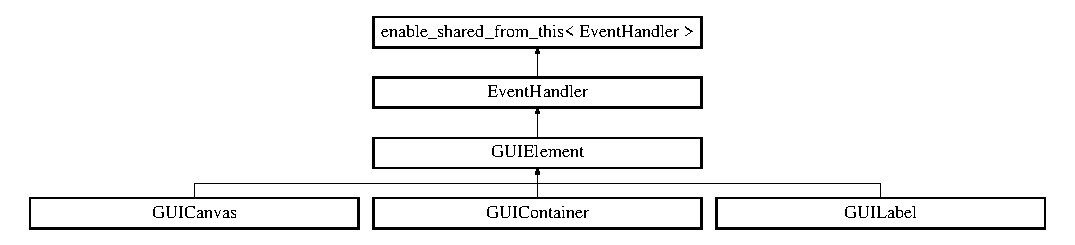
\includegraphics[height=2.839037cm]{classGUIElement}
\end{center}
\end{figure}
\subsection*{Public Member Functions}
\begin{DoxyCompactItemize}
\item 
shared\+\_\+ptr$<$ \hyperlink{classGUIElement}{G\+U\+I\+Element} $>$ \hyperlink{classGUIElement_a5ad5998c5b953b6c6e32b583ddf9cd97}{shared\+\_\+from\+\_\+this} ()
\begin{DoxyCompactList}\small\item\em Write what the function does here. \end{DoxyCompactList}\item 
shared\+\_\+ptr$<$ const \hyperlink{classGUIElement}{G\+U\+I\+Element} $>$ \hyperlink{classGUIElement_a5b381516fddb549d5db4c7bf8e6f07b0}{shared\+\_\+from\+\_\+this} () const 
\begin{DoxyCompactList}\small\item\em Write what the function does here. \end{DoxyCompactList}\item 
\hypertarget{classGUIElement_aa57dfc31bd3790306daadf9b60ffd5c9}{{\bfseries G\+U\+I\+Element} (float min\+X, float max\+X, float min\+Y, float max\+Y)}\label{classGUIElement_aa57dfc31bd3790306daadf9b60ffd5c9}

\item 
Mesh \hyperlink{classGUIElement_aeb5af965b0ea78a4699d1263690a14fa}{render} ()
\begin{DoxyCompactList}\small\item\em Write what the function does here. \end{DoxyCompactList}\item 
virtual bool \hyperlink{classGUIElement_a5f0fe42b4b9fc20f01397e7face80ae6}{is\+Point\+Inside} (float x, float y) const 
\begin{DoxyCompactList}\small\item\em Write what the function does here. \end{DoxyCompactList}\item 
virtual bool \hyperlink{classGUIElement_a073ef8863e95e55df4b701f249ba4c44}{can\+Have\+Keyboard\+Focus} () const 
\begin{DoxyCompactList}\small\item\em Write what the function does here. \end{DoxyCompactList}\item 
virtual bool \hyperlink{classGUIElement_afcccb09fab792ee06ab929dec8a9d8e7}{handle\+Mouse\+Up} (\hyperlink{structMouseUpEvent}{Mouse\+Up\+Event} \&\hyperlink{unionSDL__Event}{event}) override
\begin{DoxyCompactList}\small\item\em Write what the function does here. \end{DoxyCompactList}\item 
virtual bool \hyperlink{classGUIElement_a4809909ae2b25f816407da43b4a8f771}{handle\+Mouse\+Down} (\hyperlink{structMouseDownEvent}{Mouse\+Down\+Event} \&\hyperlink{unionSDL__Event}{event}) override
\begin{DoxyCompactList}\small\item\em Write what the function does here. \end{DoxyCompactList}\item 
virtual bool \hyperlink{classGUIElement_a82b0ee7067d1c1deaef595f312592c5a}{handle\+Mouse\+Move} (\hyperlink{structMouseMoveEvent}{Mouse\+Move\+Event} \&\hyperlink{unionSDL__Event}{event}) override
\begin{DoxyCompactList}\small\item\em Write what the function does here. \end{DoxyCompactList}\item 
virtual bool \hyperlink{classGUIElement_a0e4fe2486bff60c1dfcd058244be7acf}{handle\+Mouse\+Move\+Out} (\hyperlink{classMouseEvent}{Mouse\+Event} \&\hyperlink{unionSDL__Event}{event})
\begin{DoxyCompactList}\small\item\em Write what the function does here. \end{DoxyCompactList}\item 
virtual bool \hyperlink{classGUIElement_ae1c939c5af3544b9a5967b9035623459}{handle\+Mouse\+Move\+In} (\hyperlink{classMouseEvent}{Mouse\+Event} \&\hyperlink{unionSDL__Event}{event})
\begin{DoxyCompactList}\small\item\em Write what the function does here. \end{DoxyCompactList}\item 
virtual bool \hyperlink{classGUIElement_a3640473a7fb9651a1298122a0e0a8b29}{handle\+Mouse\+Scroll} (\hyperlink{structMouseScrollEvent}{Mouse\+Scroll\+Event} \&\hyperlink{unionSDL__Event}{event}) override
\begin{DoxyCompactList}\small\item\em Write what the function does here. \end{DoxyCompactList}\item 
virtual bool \hyperlink{classGUIElement_a7f0049f13cb199d09b6cf2e61ea8e7a3}{handle\+Key\+Up} (\hyperlink{classKeyUpEvent}{Key\+Up\+Event} \&\hyperlink{unionSDL__Event}{event}) override
\begin{DoxyCompactList}\small\item\em Write what the function does here. \end{DoxyCompactList}\item 
virtual bool \hyperlink{classGUIElement_aa85f949aa746eac4deadfa0bb8827f71}{handle\+Key\+Down} (\hyperlink{classKeyDownEvent}{Key\+Down\+Event} \&\hyperlink{unionSDL__Event}{event}) override
\begin{DoxyCompactList}\small\item\em Write what the function does here. \end{DoxyCompactList}\item 
virtual bool \hyperlink{classGUIElement_ac5b578dfd0da486e32d4cf223b2d6513}{handle\+Key\+Press} (\hyperlink{structKeyPressEvent}{Key\+Press\+Event} \&\hyperlink{unionSDL__Event}{event}) override
\begin{DoxyCompactList}\small\item\em Write what the function does here. \end{DoxyCompactList}\item 
virtual bool \hyperlink{classGUIElement_a03dc64741eed1946966776ac3af96e65}{handle\+Quit} (\hyperlink{structQuitEvent}{Quit\+Event} \&\hyperlink{unionSDL__Event}{event}) override
\begin{DoxyCompactList}\small\item\em Write what the function does here. \end{DoxyCompactList}\item 
virtual shared\+\_\+ptr$<$ \hyperlink{classGUIElement}{G\+U\+I\+Element} $>$ \hyperlink{classGUIElement_acdb491fec728f3a39318850fa144c766}{get\+Focus\+Element} ()
\begin{DoxyCompactList}\small\item\em Write what the function does here. \end{DoxyCompactList}\item 
virtual bool \hyperlink{classGUIElement_a72dffcca76f328b780c346369d7cf325}{next\+Focus\+Element} ()
\begin{DoxyCompactList}\small\item\em Write what the function does here. \end{DoxyCompactList}\item 
virtual bool \hyperlink{classGUIElement_a970e90bbb7db5de07708b0b2ef53d9e9}{prev\+Focus\+Element} ()
\begin{DoxyCompactList}\small\item\em Write what the function does here. \end{DoxyCompactList}\item 
shared\+\_\+ptr$<$ \hyperlink{classGUIContainer}{G\+U\+I\+Container} $>$ \hyperlink{classGUIElement_aded5837705c097a7a8a755df28c572e6}{get\+Parent} () const 
\begin{DoxyCompactList}\small\item\em Write what the function does here. \end{DoxyCompactList}\item 
virtual shared\+\_\+ptr$<$ \hyperlink{classGUIContainer}{G\+U\+I\+Container} $>$ \hyperlink{classGUIElement_a09eebb7ff9e98191caf3a0421f0bad8c}{get\+Top\+Level\+Parent} ()
\begin{DoxyCompactList}\small\item\em Write what the function does here. \end{DoxyCompactList}\end{DoxyCompactItemize}
\subsection*{Private Attributes}
\begin{DoxyCompactItemize}
\item 
\hypertarget{classGUIElement_a2fb7d617ff3fa7ef323cd8231e962a5a}{shared\+\_\+ptr$<$ \hyperlink{classGUIContainer}{G\+U\+I\+Container} $>$ {\bfseries parent}}\label{classGUIElement_a2fb7d617ff3fa7ef323cd8231e962a5a}

\end{DoxyCompactItemize}


\subsection{Detailed Description}
Write what the function does here. 

\begin{DoxyReturn}{Returns}

\end{DoxyReturn}


Definition at line 13 of file guielement.\+h.



\subsection{Member Function Documentation}
\hypertarget{classGUIElement_a073ef8863e95e55df4b701f249ba4c44}{\index{G\+U\+I\+Element@{G\+U\+I\+Element}!can\+Have\+Keyboard\+Focus@{can\+Have\+Keyboard\+Focus}}
\index{can\+Have\+Keyboard\+Focus@{can\+Have\+Keyboard\+Focus}!G\+U\+I\+Element@{G\+U\+I\+Element}}
\subsubsection[{can\+Have\+Keyboard\+Focus}]{\setlength{\rightskip}{0pt plus 5cm}virtual bool G\+U\+I\+Element\+::can\+Have\+Keyboard\+Focus (
\begin{DoxyParamCaption}
{}
\end{DoxyParamCaption}
) const\hspace{0.3cm}{\ttfamily [inline]}, {\ttfamily [virtual]}}}\label{classGUIElement_a073ef8863e95e55df4b701f249ba4c44}


Write what the function does here. 

\begin{DoxyReturn}{Returns}

\end{DoxyReturn}


Reimplemented in \hyperlink{classGUIContainer_a54bbf86cc92ce6518ccdc25a21b8e5f5}{G\+U\+I\+Container}, and \hyperlink{structGUILabel_aa0127a15c722bc35de3441e8d2952a28}{G\+U\+I\+Label}.



Definition at line 69 of file guielement.\+h.


\begin{DoxyCode}
70         \{
71             \textcolor{keywordflow}{return} \textcolor{keyword}{false};
72         \}
\end{DoxyCode}
\hypertarget{classGUIElement_acdb491fec728f3a39318850fa144c766}{\index{G\+U\+I\+Element@{G\+U\+I\+Element}!get\+Focus\+Element@{get\+Focus\+Element}}
\index{get\+Focus\+Element@{get\+Focus\+Element}!G\+U\+I\+Element@{G\+U\+I\+Element}}
\subsubsection[{get\+Focus\+Element}]{\setlength{\rightskip}{0pt plus 5cm}virtual shared\+\_\+ptr$<${\bf G\+U\+I\+Element}$>$ G\+U\+I\+Element\+::get\+Focus\+Element (
\begin{DoxyParamCaption}
{}
\end{DoxyParamCaption}
)\hspace{0.3cm}{\ttfamily [inline]}, {\ttfamily [virtual]}}}\label{classGUIElement_acdb491fec728f3a39318850fa144c766}


Write what the function does here. 

\begin{DoxyReturn}{Returns}

\end{DoxyReturn}


Reimplemented in \hyperlink{classGUIContainer_addf987ba650075a7c0f34c571debd6a2}{G\+U\+I\+Container}.



Definition at line 200 of file guielement.\+h.



References shared\+\_\+from\+\_\+this().


\begin{DoxyCode}
201         \{
202             \textcolor{keywordflow}{return} \hyperlink{classGUIElement_a5ad5998c5b953b6c6e32b583ddf9cd97}{shared\_from\_this}();
203         \}
\end{DoxyCode}
\hypertarget{classGUIElement_aded5837705c097a7a8a755df28c572e6}{\index{G\+U\+I\+Element@{G\+U\+I\+Element}!get\+Parent@{get\+Parent}}
\index{get\+Parent@{get\+Parent}!G\+U\+I\+Element@{G\+U\+I\+Element}}
\subsubsection[{get\+Parent}]{\setlength{\rightskip}{0pt plus 5cm}shared\+\_\+ptr$<${\bf G\+U\+I\+Container}$>$ G\+U\+I\+Element\+::get\+Parent (
\begin{DoxyParamCaption}
{}
\end{DoxyParamCaption}
) const\hspace{0.3cm}{\ttfamily [inline]}}}\label{classGUIElement_aded5837705c097a7a8a755df28c572e6}


Write what the function does here. 

virtual void first\+Focus\+Element() \{ \}

/$\ast$$\ast$ Write what the function does here

virtual void last\+Focus\+Element() \{ \} void set\+Focus(); float min\+X, max\+X, min\+Y, max\+Y;

/$\ast$$\ast$ Write what the function does here

virtual void reset() \{ \} protected\+: virtual Mesh render(float min\+Z, float max\+Z, bool has\+Focus) = 0; friend class \hyperlink{classGUIContainer}{G\+U\+I\+Container}; // so \hyperlink{classGUIContainer}{G\+U\+I\+Container} can set parent friend class \hyperlink{classGUIRunner}{G\+U\+I\+Runner};

/$\ast$$\ast$ Write what the function does here

\begin{DoxyReturn}{Returns}

\end{DoxyReturn}


Definition at line 257 of file guielement.\+h.


\begin{DoxyCode}
258         \{
259             \textcolor{keywordflow}{return} parent;
260         \}
\end{DoxyCode}
\hypertarget{classGUIElement_a09eebb7ff9e98191caf3a0421f0bad8c}{\index{G\+U\+I\+Element@{G\+U\+I\+Element}!get\+Top\+Level\+Parent@{get\+Top\+Level\+Parent}}
\index{get\+Top\+Level\+Parent@{get\+Top\+Level\+Parent}!G\+U\+I\+Element@{G\+U\+I\+Element}}
\subsubsection[{get\+Top\+Level\+Parent}]{\setlength{\rightskip}{0pt plus 5cm}shared\+\_\+ptr$<$ {\bf G\+U\+I\+Container} $>$ G\+U\+I\+Element\+::get\+Top\+Level\+Parent (
\begin{DoxyParamCaption}
{}
\end{DoxyParamCaption}
)\hspace{0.3cm}{\ttfamily [inline]}, {\ttfamily [virtual]}}}\label{classGUIElement_a09eebb7ff9e98191caf3a0421f0bad8c}


Write what the function does here. 

\begin{DoxyReturn}{Returns}

\end{DoxyReturn}


Reimplemented in \hyperlink{classGUIContainer_a4bade45ffb4a8961ba2a3e0b406d186c}{G\+U\+I\+Container}.



Definition at line 614 of file guicontainer.\+h.


\begin{DoxyCode}
615 \{
616     shared\_ptr<GUIContainer> retval = \hyperlink{classGUIElement_aded5837705c097a7a8a755df28c572e6}{getParent}();
617     \textcolor{keywordflow}{if}(retval == \textcolor{keyword}{nullptr})
618         \textcolor{keywordflow}{return} retval;
619     \textcolor{keywordflow}{while}(retval->getParent() != \textcolor{keyword}{nullptr})
620         retval = retval->getParent();
621     \textcolor{keywordflow}{return} retval;
622 \}
\end{DoxyCode}
\hypertarget{classGUIElement_aa85f949aa746eac4deadfa0bb8827f71}{\index{G\+U\+I\+Element@{G\+U\+I\+Element}!handle\+Key\+Down@{handle\+Key\+Down}}
\index{handle\+Key\+Down@{handle\+Key\+Down}!G\+U\+I\+Element@{G\+U\+I\+Element}}
\subsubsection[{handle\+Key\+Down}]{\setlength{\rightskip}{0pt plus 5cm}virtual bool G\+U\+I\+Element\+::handle\+Key\+Down (
\begin{DoxyParamCaption}
\item[{{\bf Key\+Down\+Event} \&}]{event}
\end{DoxyParamCaption}
)\hspace{0.3cm}{\ttfamily [inline]}, {\ttfamily [override]}, {\ttfamily [virtual]}}}\label{classGUIElement_aa85f949aa746eac4deadfa0bb8827f71}


Write what the function does here. 


\begin{DoxyParams}{Parameters}
{\em event} & \\
\hline
\end{DoxyParams}
\begin{DoxyReturn}{Returns}

\end{DoxyReturn}


Implements \hyperlink{structEventHandler}{Event\+Handler}.



Reimplemented in \hyperlink{classGUIContainer_a8dec7de665719cb1e440a655fac6b69a}{G\+U\+I\+Container}.



Definition at line 166 of file guielement.\+h.


\begin{DoxyCode}
167         \{
168             \textcolor{keywordflow}{return} \textcolor{keyword}{false};
169         \}
\end{DoxyCode}
\hypertarget{classGUIElement_ac5b578dfd0da486e32d4cf223b2d6513}{\index{G\+U\+I\+Element@{G\+U\+I\+Element}!handle\+Key\+Press@{handle\+Key\+Press}}
\index{handle\+Key\+Press@{handle\+Key\+Press}!G\+U\+I\+Element@{G\+U\+I\+Element}}
\subsubsection[{handle\+Key\+Press}]{\setlength{\rightskip}{0pt plus 5cm}virtual bool G\+U\+I\+Element\+::handle\+Key\+Press (
\begin{DoxyParamCaption}
\item[{{\bf Key\+Press\+Event} \&}]{event}
\end{DoxyParamCaption}
)\hspace{0.3cm}{\ttfamily [inline]}, {\ttfamily [override]}, {\ttfamily [virtual]}}}\label{classGUIElement_ac5b578dfd0da486e32d4cf223b2d6513}


Write what the function does here. 


\begin{DoxyParams}{Parameters}
{\em event} & \\
\hline
\end{DoxyParams}
\begin{DoxyReturn}{Returns}

\end{DoxyReturn}


Implements \hyperlink{structEventHandler}{Event\+Handler}.



Reimplemented in \hyperlink{classGUIContainer_a7109d4597eb95baa047e4de213f9428f}{G\+U\+I\+Container}.



Definition at line 178 of file guielement.\+h.


\begin{DoxyCode}
179         \{
180             \textcolor{keywordflow}{return} \textcolor{keyword}{false};
181         \}
\end{DoxyCode}
\hypertarget{classGUIElement_a7f0049f13cb199d09b6cf2e61ea8e7a3}{\index{G\+U\+I\+Element@{G\+U\+I\+Element}!handle\+Key\+Up@{handle\+Key\+Up}}
\index{handle\+Key\+Up@{handle\+Key\+Up}!G\+U\+I\+Element@{G\+U\+I\+Element}}
\subsubsection[{handle\+Key\+Up}]{\setlength{\rightskip}{0pt plus 5cm}virtual bool G\+U\+I\+Element\+::handle\+Key\+Up (
\begin{DoxyParamCaption}
\item[{{\bf Key\+Up\+Event} \&}]{event}
\end{DoxyParamCaption}
)\hspace{0.3cm}{\ttfamily [inline]}, {\ttfamily [override]}, {\ttfamily [virtual]}}}\label{classGUIElement_a7f0049f13cb199d09b6cf2e61ea8e7a3}


Write what the function does here. 


\begin{DoxyParams}{Parameters}
{\em event} & \\
\hline
\end{DoxyParams}
\begin{DoxyReturn}{Returns}

\end{DoxyReturn}


Implements \hyperlink{structEventHandler}{Event\+Handler}.



Reimplemented in \hyperlink{classGUIContainer_a6e1ad46740bab18d77efb8f88c3a70bb}{G\+U\+I\+Container}.



Definition at line 154 of file guielement.\+h.


\begin{DoxyCode}
155         \{
156             \textcolor{keywordflow}{return} \textcolor{keyword}{false};
157         \}
\end{DoxyCode}
\hypertarget{classGUIElement_a4809909ae2b25f816407da43b4a8f771}{\index{G\+U\+I\+Element@{G\+U\+I\+Element}!handle\+Mouse\+Down@{handle\+Mouse\+Down}}
\index{handle\+Mouse\+Down@{handle\+Mouse\+Down}!G\+U\+I\+Element@{G\+U\+I\+Element}}
\subsubsection[{handle\+Mouse\+Down}]{\setlength{\rightskip}{0pt plus 5cm}virtual bool G\+U\+I\+Element\+::handle\+Mouse\+Down (
\begin{DoxyParamCaption}
\item[{{\bf Mouse\+Down\+Event} \&}]{event}
\end{DoxyParamCaption}
)\hspace{0.3cm}{\ttfamily [inline]}, {\ttfamily [override]}, {\ttfamily [virtual]}}}\label{classGUIElement_a4809909ae2b25f816407da43b4a8f771}


Write what the function does here. 


\begin{DoxyParams}{Parameters}
{\em event} & \\
\hline
\end{DoxyParams}
\begin{DoxyReturn}{Returns}

\end{DoxyReturn}


Implements \hyperlink{structEventHandler}{Event\+Handler}.



Reimplemented in \hyperlink{classGUIContainer_a10229d26c8bdac0e8b1c3b0e2863331a}{G\+U\+I\+Container}.



Definition at line 93 of file guielement.\+h.


\begin{DoxyCode}
94         \{
95             setFocus();
96             \textcolor{keywordflow}{return} \textcolor{keyword}{true};
97         \}
\end{DoxyCode}
\hypertarget{classGUIElement_a82b0ee7067d1c1deaef595f312592c5a}{\index{G\+U\+I\+Element@{G\+U\+I\+Element}!handle\+Mouse\+Move@{handle\+Mouse\+Move}}
\index{handle\+Mouse\+Move@{handle\+Mouse\+Move}!G\+U\+I\+Element@{G\+U\+I\+Element}}
\subsubsection[{handle\+Mouse\+Move}]{\setlength{\rightskip}{0pt plus 5cm}virtual bool G\+U\+I\+Element\+::handle\+Mouse\+Move (
\begin{DoxyParamCaption}
\item[{{\bf Mouse\+Move\+Event} \&}]{event}
\end{DoxyParamCaption}
)\hspace{0.3cm}{\ttfamily [inline]}, {\ttfamily [override]}, {\ttfamily [virtual]}}}\label{classGUIElement_a82b0ee7067d1c1deaef595f312592c5a}


Write what the function does here. 


\begin{DoxyParams}{Parameters}
{\em event} & \\
\hline
\end{DoxyParams}
\begin{DoxyReturn}{Returns}

\end{DoxyReturn}


Implements \hyperlink{structEventHandler}{Event\+Handler}.



Reimplemented in \hyperlink{classGUIContainer_a9ee4ac638a114d858ab8836fb3dde441}{G\+U\+I\+Container}.



Definition at line 106 of file guielement.\+h.


\begin{DoxyCode}
107         \{
108             \textcolor{keywordflow}{return} \textcolor{keyword}{true};
109         \}
\end{DoxyCode}
\hypertarget{classGUIElement_ae1c939c5af3544b9a5967b9035623459}{\index{G\+U\+I\+Element@{G\+U\+I\+Element}!handle\+Mouse\+Move\+In@{handle\+Mouse\+Move\+In}}
\index{handle\+Mouse\+Move\+In@{handle\+Mouse\+Move\+In}!G\+U\+I\+Element@{G\+U\+I\+Element}}
\subsubsection[{handle\+Mouse\+Move\+In}]{\setlength{\rightskip}{0pt plus 5cm}virtual bool G\+U\+I\+Element\+::handle\+Mouse\+Move\+In (
\begin{DoxyParamCaption}
\item[{{\bf Mouse\+Event} \&}]{event}
\end{DoxyParamCaption}
)\hspace{0.3cm}{\ttfamily [inline]}, {\ttfamily [virtual]}}}\label{classGUIElement_ae1c939c5af3544b9a5967b9035623459}


Write what the function does here. 


\begin{DoxyParams}{Parameters}
{\em event} & \\
\hline
\end{DoxyParams}
\begin{DoxyReturn}{Returns}

\end{DoxyReturn}


Reimplemented in \hyperlink{classGUIContainer_a5de801e62c8d14d559e3dfae68cca72d}{G\+U\+I\+Container}.



Definition at line 130 of file guielement.\+h.


\begin{DoxyCode}
131         \{
132             \textcolor{keywordflow}{return} \textcolor{keyword}{true};
133         \}
\end{DoxyCode}
\hypertarget{classGUIElement_a0e4fe2486bff60c1dfcd058244be7acf}{\index{G\+U\+I\+Element@{G\+U\+I\+Element}!handle\+Mouse\+Move\+Out@{handle\+Mouse\+Move\+Out}}
\index{handle\+Mouse\+Move\+Out@{handle\+Mouse\+Move\+Out}!G\+U\+I\+Element@{G\+U\+I\+Element}}
\subsubsection[{handle\+Mouse\+Move\+Out}]{\setlength{\rightskip}{0pt plus 5cm}virtual bool G\+U\+I\+Element\+::handle\+Mouse\+Move\+Out (
\begin{DoxyParamCaption}
\item[{{\bf Mouse\+Event} \&}]{event}
\end{DoxyParamCaption}
)\hspace{0.3cm}{\ttfamily [inline]}, {\ttfamily [virtual]}}}\label{classGUIElement_a0e4fe2486bff60c1dfcd058244be7acf}


Write what the function does here. 


\begin{DoxyParams}{Parameters}
{\em event} & \\
\hline
\end{DoxyParams}
\begin{DoxyReturn}{Returns}

\end{DoxyReturn}


Reimplemented in \hyperlink{classGUIContainer_a85ef65ef4de74236bb2b5f200636fa0c}{G\+U\+I\+Container}.



Definition at line 118 of file guielement.\+h.


\begin{DoxyCode}
119         \{
120             \textcolor{keywordflow}{return} \textcolor{keyword}{true};
121         \}
\end{DoxyCode}
\hypertarget{classGUIElement_a3640473a7fb9651a1298122a0e0a8b29}{\index{G\+U\+I\+Element@{G\+U\+I\+Element}!handle\+Mouse\+Scroll@{handle\+Mouse\+Scroll}}
\index{handle\+Mouse\+Scroll@{handle\+Mouse\+Scroll}!G\+U\+I\+Element@{G\+U\+I\+Element}}
\subsubsection[{handle\+Mouse\+Scroll}]{\setlength{\rightskip}{0pt plus 5cm}virtual bool G\+U\+I\+Element\+::handle\+Mouse\+Scroll (
\begin{DoxyParamCaption}
\item[{{\bf Mouse\+Scroll\+Event} \&}]{event}
\end{DoxyParamCaption}
)\hspace{0.3cm}{\ttfamily [inline]}, {\ttfamily [override]}, {\ttfamily [virtual]}}}\label{classGUIElement_a3640473a7fb9651a1298122a0e0a8b29}


Write what the function does here. 


\begin{DoxyParams}{Parameters}
{\em event} & \\
\hline
\end{DoxyParams}
\begin{DoxyReturn}{Returns}

\end{DoxyReturn}


Implements \hyperlink{structEventHandler}{Event\+Handler}.



Reimplemented in \hyperlink{classGUIContainer_a80a3c99fbdec76ac9a333a6737e9ff5a}{G\+U\+I\+Container}.



Definition at line 142 of file guielement.\+h.


\begin{DoxyCode}
143         \{
144             \textcolor{keywordflow}{return} \textcolor{keyword}{false};
145         \}
\end{DoxyCode}
\hypertarget{classGUIElement_afcccb09fab792ee06ab929dec8a9d8e7}{\index{G\+U\+I\+Element@{G\+U\+I\+Element}!handle\+Mouse\+Up@{handle\+Mouse\+Up}}
\index{handle\+Mouse\+Up@{handle\+Mouse\+Up}!G\+U\+I\+Element@{G\+U\+I\+Element}}
\subsubsection[{handle\+Mouse\+Up}]{\setlength{\rightskip}{0pt plus 5cm}virtual bool G\+U\+I\+Element\+::handle\+Mouse\+Up (
\begin{DoxyParamCaption}
\item[{{\bf Mouse\+Up\+Event} \&}]{event}
\end{DoxyParamCaption}
)\hspace{0.3cm}{\ttfamily [inline]}, {\ttfamily [override]}, {\ttfamily [virtual]}}}\label{classGUIElement_afcccb09fab792ee06ab929dec8a9d8e7}


Write what the function does here. 


\begin{DoxyParams}{Parameters}
{\em event} & \\
\hline
\end{DoxyParams}
\begin{DoxyReturn}{Returns}

\end{DoxyReturn}


Implements \hyperlink{structEventHandler}{Event\+Handler}.



Reimplemented in \hyperlink{classGUIContainer_acba4796c4bec859c70f04a4f4471b3fe}{G\+U\+I\+Container}.



Definition at line 81 of file guielement.\+h.


\begin{DoxyCode}
82         \{
83             \textcolor{keywordflow}{return} \textcolor{keyword}{true};
84         \}
\end{DoxyCode}
\hypertarget{classGUIElement_a03dc64741eed1946966776ac3af96e65}{\index{G\+U\+I\+Element@{G\+U\+I\+Element}!handle\+Quit@{handle\+Quit}}
\index{handle\+Quit@{handle\+Quit}!G\+U\+I\+Element@{G\+U\+I\+Element}}
\subsubsection[{handle\+Quit}]{\setlength{\rightskip}{0pt plus 5cm}virtual bool G\+U\+I\+Element\+::handle\+Quit (
\begin{DoxyParamCaption}
\item[{{\bf Quit\+Event} \&}]{event}
\end{DoxyParamCaption}
)\hspace{0.3cm}{\ttfamily [inline]}, {\ttfamily [override]}, {\ttfamily [virtual]}}}\label{classGUIElement_a03dc64741eed1946966776ac3af96e65}


Write what the function does here. 


\begin{DoxyParams}{Parameters}
{\em event} & \\
\hline
\end{DoxyParams}
\begin{DoxyReturn}{Returns}

\end{DoxyReturn}


Implements \hyperlink{structEventHandler}{Event\+Handler}.



Reimplemented in \hyperlink{classGUIContainer_a1fbd8dfea04418ce139b202961987255}{G\+U\+I\+Container}.



Definition at line 190 of file guielement.\+h.


\begin{DoxyCode}
191         \{
192             \textcolor{keywordflow}{return} \textcolor{keyword}{false};
193         \}
\end{DoxyCode}
\hypertarget{classGUIElement_a5f0fe42b4b9fc20f01397e7face80ae6}{\index{G\+U\+I\+Element@{G\+U\+I\+Element}!is\+Point\+Inside@{is\+Point\+Inside}}
\index{is\+Point\+Inside@{is\+Point\+Inside}!G\+U\+I\+Element@{G\+U\+I\+Element}}
\subsubsection[{is\+Point\+Inside}]{\setlength{\rightskip}{0pt plus 5cm}virtual bool G\+U\+I\+Element\+::is\+Point\+Inside (
\begin{DoxyParamCaption}
\item[{float}]{x, }
\item[{float}]{y}
\end{DoxyParamCaption}
) const\hspace{0.3cm}{\ttfamily [inline]}, {\ttfamily [virtual]}}}\label{classGUIElement_a5f0fe42b4b9fc20f01397e7face80ae6}


Write what the function does here. 


\begin{DoxyParams}{Parameters}
{\em x} & \\
\hline
{\em y} & \\
\hline
\end{DoxyParams}
\begin{DoxyReturn}{Returns}

\end{DoxyReturn}


Definition at line 57 of file guielement.\+h.


\begin{DoxyCode}
58         \{
59             \textcolor{keywordflow}{if}(x < minX || x > maxX || y < minY || y > maxY)
60                 \textcolor{keywordflow}{return} \textcolor{keyword}{false};
61             \textcolor{keywordflow}{return} \textcolor{keyword}{true};
62         \}
\end{DoxyCode}
\hypertarget{classGUIElement_a72dffcca76f328b780c346369d7cf325}{\index{G\+U\+I\+Element@{G\+U\+I\+Element}!next\+Focus\+Element@{next\+Focus\+Element}}
\index{next\+Focus\+Element@{next\+Focus\+Element}!G\+U\+I\+Element@{G\+U\+I\+Element}}
\subsubsection[{next\+Focus\+Element}]{\setlength{\rightskip}{0pt plus 5cm}virtual bool G\+U\+I\+Element\+::next\+Focus\+Element (
\begin{DoxyParamCaption}
{}
\end{DoxyParamCaption}
)\hspace{0.3cm}{\ttfamily [inline]}, {\ttfamily [virtual]}}}\label{classGUIElement_a72dffcca76f328b780c346369d7cf325}


Write what the function does here. 

true when reached container boundary 

Reimplemented in \hyperlink{classGUIContainer_a83c20737ae89ecdb0da054cec1ca087e}{G\+U\+I\+Container}.



Definition at line 210 of file guielement.\+h.


\begin{DoxyCode}
211         \{
212             \textcolor{keywordflow}{return} \textcolor{keyword}{true};
213         \}
\end{DoxyCode}
\hypertarget{classGUIElement_a970e90bbb7db5de07708b0b2ef53d9e9}{\index{G\+U\+I\+Element@{G\+U\+I\+Element}!prev\+Focus\+Element@{prev\+Focus\+Element}}
\index{prev\+Focus\+Element@{prev\+Focus\+Element}!G\+U\+I\+Element@{G\+U\+I\+Element}}
\subsubsection[{prev\+Focus\+Element}]{\setlength{\rightskip}{0pt plus 5cm}virtual bool G\+U\+I\+Element\+::prev\+Focus\+Element (
\begin{DoxyParamCaption}
{}
\end{DoxyParamCaption}
)\hspace{0.3cm}{\ttfamily [inline]}, {\ttfamily [virtual]}}}\label{classGUIElement_a970e90bbb7db5de07708b0b2ef53d9e9}


Write what the function does here. 

true when reached container boundary 

Reimplemented in \hyperlink{classGUIContainer_afa186df2611c4e309094e8da2654f5b2}{G\+U\+I\+Container}.



Definition at line 220 of file guielement.\+h.


\begin{DoxyCode}
221         \{
222             \textcolor{keywordflow}{return} \textcolor{keyword}{true};
223         \}
\end{DoxyCode}
\hypertarget{classGUIElement_aeb5af965b0ea78a4699d1263690a14fa}{\index{G\+U\+I\+Element@{G\+U\+I\+Element}!render@{render}}
\index{render@{render}!G\+U\+I\+Element@{G\+U\+I\+Element}}
\subsubsection[{render}]{\setlength{\rightskip}{0pt plus 5cm}Mesh G\+U\+I\+Element\+::render (
\begin{DoxyParamCaption}
{}
\end{DoxyParamCaption}
)\hspace{0.3cm}{\ttfamily [inline]}}}\label{classGUIElement_aeb5af965b0ea78a4699d1263690a14fa}


Write what the function does here. 

\begin{DoxyReturn}{Returns}

\end{DoxyReturn}


Definition at line 44 of file guielement.\+h.


\begin{DoxyCode}
45         \{
46             \textcolor{keywordflow}{return} \hyperlink{classGUIElement_aeb5af965b0ea78a4699d1263690a14fa}{render}(0.1, 10, \textcolor{keyword}{true});
47         \}
\end{DoxyCode}
\hypertarget{classGUIElement_a5ad5998c5b953b6c6e32b583ddf9cd97}{\index{G\+U\+I\+Element@{G\+U\+I\+Element}!shared\+\_\+from\+\_\+this@{shared\+\_\+from\+\_\+this}}
\index{shared\+\_\+from\+\_\+this@{shared\+\_\+from\+\_\+this}!G\+U\+I\+Element@{G\+U\+I\+Element}}
\subsubsection[{shared\+\_\+from\+\_\+this}]{\setlength{\rightskip}{0pt plus 5cm}shared\+\_\+ptr$<${\bf G\+U\+I\+Element}$>$ G\+U\+I\+Element\+::shared\+\_\+from\+\_\+this (
\begin{DoxyParamCaption}
{}
\end{DoxyParamCaption}
)\hspace{0.3cm}{\ttfamily [inline]}}}\label{classGUIElement_a5ad5998c5b953b6c6e32b583ddf9cd97}


Write what the function does here. 

\begin{DoxyReturn}{Returns}

\end{DoxyReturn}


Definition at line 22 of file guielement.\+h.



Referenced by get\+Focus\+Element().


\begin{DoxyCode}
23         \{
24             \textcolor{keywordflow}{return} dynamic\_pointer\_cast<\hyperlink{classGUIElement}{GUIElement}>(EventHandler::shared\_from\_this());
25         \}
\end{DoxyCode}
\hypertarget{classGUIElement_a5b381516fddb549d5db4c7bf8e6f07b0}{\index{G\+U\+I\+Element@{G\+U\+I\+Element}!shared\+\_\+from\+\_\+this@{shared\+\_\+from\+\_\+this}}
\index{shared\+\_\+from\+\_\+this@{shared\+\_\+from\+\_\+this}!G\+U\+I\+Element@{G\+U\+I\+Element}}
\subsubsection[{shared\+\_\+from\+\_\+this}]{\setlength{\rightskip}{0pt plus 5cm}shared\+\_\+ptr$<$const {\bf G\+U\+I\+Element}$>$ G\+U\+I\+Element\+::shared\+\_\+from\+\_\+this (
\begin{DoxyParamCaption}
{}
\end{DoxyParamCaption}
) const\hspace{0.3cm}{\ttfamily [inline]}}}\label{classGUIElement_a5b381516fddb549d5db4c7bf8e6f07b0}


Write what the function does here. 

\begin{DoxyReturn}{Returns}

\end{DoxyReturn}


Definition at line 32 of file guielement.\+h.


\begin{DoxyCode}
33         \{
34             \textcolor{keywordflow}{return} dynamic\_pointer\_cast<\textcolor{keyword}{const} \hyperlink{classGUIElement}{GUIElement}>(EventHandler::shared\_from\_this());
35         \}
\end{DoxyCode}


The documentation for this class was generated from the following files\+:\begin{DoxyCompactItemize}
\item 
guielement.\+h\item 
guicontainer.\+h\item 
guielement.\+cpp\end{DoxyCompactItemize}

\hypertarget{structGUILabel}{\section{G\+U\+I\+Label Struct Reference}
\label{structGUILabel}\index{G\+U\+I\+Label@{G\+U\+I\+Label}}
}


Write what the function does here.  




{\ttfamily \#include $<$guilabel.\+h$>$}

Inheritance diagram for G\+U\+I\+Label\+:\begin{figure}[H]
\begin{center}
\leavevmode
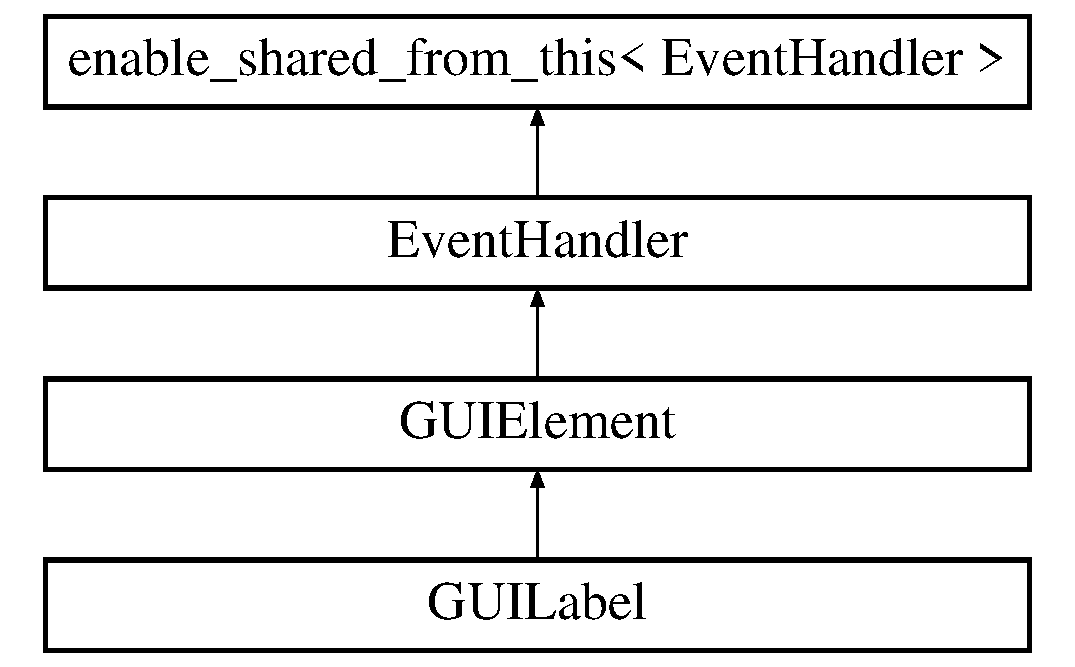
\includegraphics[height=4.000000cm]{structGUILabel}
\end{center}
\end{figure}
\subsection*{Public Member Functions}
\begin{DoxyCompactItemize}
\item 
\hypertarget{structGUILabel_ac4d7442b38260774b14536b343f4ff51}{{\bfseries G\+U\+I\+Label} (wstring text, float min\+X, float max\+X, float min\+Y, float max\+Y, \hyperlink{structColor}{Color} text\+Color=\hyperlink{structColor_a723061c1cca0072a8ecb591c4c3b4479}{Color\+::\+V}(0))}\label{structGUILabel_ac4d7442b38260774b14536b343f4ff51}

\item 
virtual bool \hyperlink{structGUILabel_aa0127a15c722bc35de3441e8d2952a28}{can\+Have\+Keyboard\+Focus} () const overridefinal
\begin{DoxyCompactList}\small\item\em Write what the function does here. \end{DoxyCompactList}\end{DoxyCompactItemize}
\subsection*{Public Attributes}
\begin{DoxyCompactItemize}
\item 
\hypertarget{structGUILabel_a455ecc85732712f002fce8dcb4f8b0db}{wstring {\bfseries text}}\label{structGUILabel_a455ecc85732712f002fce8dcb4f8b0db}

\item 
\hypertarget{structGUILabel_a6ecebb11c95e284a76e706d774966067}{\hyperlink{structColor}{Color} {\bfseries text\+Color}}\label{structGUILabel_a6ecebb11c95e284a76e706d774966067}

\end{DoxyCompactItemize}
\subsection*{Protected Member Functions}
\begin{DoxyCompactItemize}
\item 
virtual Mesh \hyperlink{structGUILabel_a1b53ad7ce5ea0d2f3bbd6289636d95c3}{render} (float min\+Z, float max\+Z, bool has\+Focus) override
\begin{DoxyCompactList}\small\item\em Write what the function does here. \end{DoxyCompactList}\end{DoxyCompactItemize}


\subsection{Detailed Description}
Write what the function does here. 

\begin{DoxyReturn}{Returns}

\end{DoxyReturn}


Definition at line 15 of file guilabel.\+h.



\subsection{Member Function Documentation}
\hypertarget{structGUILabel_aa0127a15c722bc35de3441e8d2952a28}{\index{G\+U\+I\+Label@{G\+U\+I\+Label}!can\+Have\+Keyboard\+Focus@{can\+Have\+Keyboard\+Focus}}
\index{can\+Have\+Keyboard\+Focus@{can\+Have\+Keyboard\+Focus}!G\+U\+I\+Label@{G\+U\+I\+Label}}
\subsubsection[{can\+Have\+Keyboard\+Focus}]{\setlength{\rightskip}{0pt plus 5cm}virtual bool G\+U\+I\+Label\+::can\+Have\+Keyboard\+Focus (
\begin{DoxyParamCaption}
{}
\end{DoxyParamCaption}
) const\hspace{0.3cm}{\ttfamily [inline]}, {\ttfamily [final]}, {\ttfamily [override]}, {\ttfamily [virtual]}}}\label{structGUILabel_aa0127a15c722bc35de3441e8d2952a28}


Write what the function does here. 

\begin{DoxyReturn}{Returns}

\end{DoxyReturn}


Reimplemented from \hyperlink{classGUIElement_a073ef8863e95e55df4b701f249ba4c44}{G\+U\+I\+Element}.



Definition at line 29 of file guilabel.\+h.


\begin{DoxyCode}
30     \{
31         \textcolor{keywordflow}{return} \textcolor{keyword}{false};
32     \}
\end{DoxyCode}
\hypertarget{structGUILabel_a1b53ad7ce5ea0d2f3bbd6289636d95c3}{\index{G\+U\+I\+Label@{G\+U\+I\+Label}!render@{render}}
\index{render@{render}!G\+U\+I\+Label@{G\+U\+I\+Label}}
\subsubsection[{render}]{\setlength{\rightskip}{0pt plus 5cm}virtual Mesh G\+U\+I\+Label\+::render (
\begin{DoxyParamCaption}
\item[{float}]{min\+Z, }
\item[{float}]{max\+Z, }
\item[{bool}]{has\+Focus}
\end{DoxyParamCaption}
)\hspace{0.3cm}{\ttfamily [inline]}, {\ttfamily [override]}, {\ttfamily [protected]}, {\ttfamily [virtual]}}}\label{structGUILabel_a1b53ad7ce5ea0d2f3bbd6289636d95c3}


Write what the function does here. 


\begin{DoxyParams}{Parameters}
{\em min\+Z} & \\
\hline
{\em max\+Z} & \\
\hline
{\em has\+Focus} & \\
\hline
\end{DoxyParams}
\begin{DoxyReturn}{Returns}

\end{DoxyReturn}


Definition at line 44 of file guilabel.\+h.



References Matrix\+::scale(), and Matrix\+::translate().


\begin{DoxyCode}
45     \{
46         \textcolor{keywordtype}{float} textWidth = Text::width(text);
47         \textcolor{keywordtype}{float} textHeight = Text::height(text);
48         \textcolor{keywordflow}{if}(textWidth == 0)
49             textWidth = 1;
50         \textcolor{keywordflow}{if}(textHeight == 0)
51             textHeight = 1;
52         \textcolor{keywordtype}{float} textScale = 0.5 * (maxY - minY) / textHeight;
53         textScale = min(textScale, (maxX - minX) / textWidth);
54         \textcolor{keywordtype}{float} xOffset = -0.5 * textWidth, yOffset = -0.5 * textHeight;
55         xOffset = textScale * xOffset + 0.5 * (minX + maxX);
56         yOffset = textScale * yOffset + 0.5 * (minY + maxY);
57         \textcolor{keywordflow}{return} (Mesh)transform(\hyperlink{classMatrix_a1f36f7f62b8e99fea99880b6fc80a604}{Matrix::scale}(textScale).concat(
      \hyperlink{classMatrix_adf246c47bce77c3c53b9e804ec475e35}{Matrix::translate}(xOffset, yOffset, -1).concat(\hyperlink{classMatrix_a1f36f7f62b8e99fea99880b6fc80a604}{Matrix::scale}(minZ))), 
      Text::mesh(text, textColor));
58     \}
\end{DoxyCode}


The documentation for this struct was generated from the following file\+:\begin{DoxyCompactItemize}
\item 
guilabel.\+h\end{DoxyCompactItemize}

\hypertarget{classGUIRunner}{\section{G\+U\+I\+Runner Class Reference}
\label{classGUIRunner}\index{G\+U\+I\+Runner@{G\+U\+I\+Runner}}
}


Write what the function does here.  




{\ttfamily \#include $<$gui.\+h$>$}

Inheritance diagram for G\+U\+I\+Runner\+:\begin{figure}[H]
\begin{center}
\leavevmode
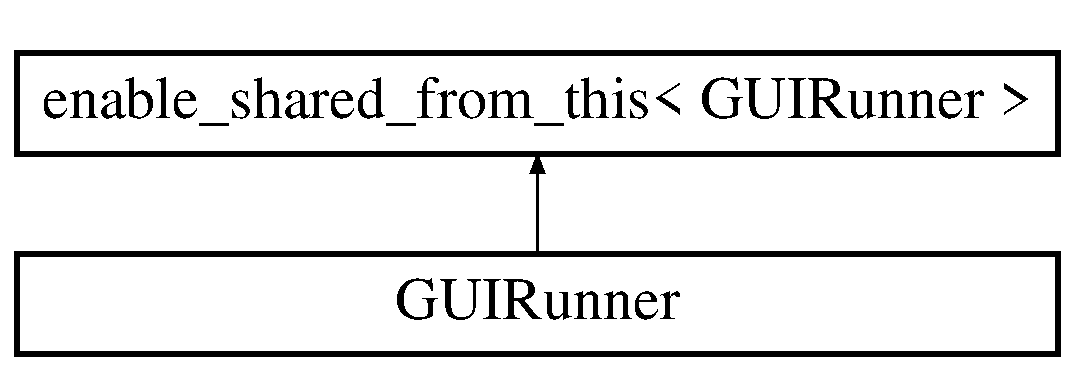
\includegraphics[height=2.000000cm]{classGUIRunner}
\end{center}
\end{figure}
\subsection*{Public Member Functions}
\begin{DoxyCompactItemize}
\item 
\hyperlink{classGUIRunner_aede15735ddb1dfdde334cfa6a4263c8d}{$\sim$\+G\+U\+I\+Runner} ()
\begin{DoxyCompactList}\small\item\em Write what the function does here. \end{DoxyCompactList}\item 
\hypertarget{classGUIRunner_aa573be0a5f5473f5a7fe492eb2d94894}{bool {\bfseries run} ()}\label{classGUIRunner_aa573be0a5f5473f5a7fe492eb2d94894}

\item 
void \hyperlink{classGUIRunner_a71350d287889af5d9e588af1361390d0}{schedule\+Function} (function$<$ void()$>$ fn)
\begin{DoxyCompactList}\small\item\em Write what the function does here. \end{DoxyCompactList}\item 
void \hyperlink{classGUIRunner_a516b306d0c8ba1ba979db12947ea5541}{quit} (bool retval=false)
\begin{DoxyCompactList}\small\item\em Write what the function does here. \end{DoxyCompactList}\item 
shared\+\_\+ptr$<$ \hyperlink{classGUIContainer}{G\+U\+I\+Container} $>$ \hyperlink{classGUIRunner_a9c09adda078b10a901dacb17fae7d888}{get\+G\+U\+I} ()
\begin{DoxyCompactList}\small\item\em Write what the function does here. \end{DoxyCompactList}\end{DoxyCompactItemize}
\subsection*{Static Public Member Functions}
\begin{DoxyCompactItemize}
\item 
static shared\+\_\+ptr$<$ \hyperlink{classGUIRunner}{G\+U\+I\+Runner} $>$ \hyperlink{classGUIRunner_a75d10817e13347f279c658ef35e18686}{make} (shared\+\_\+ptr$<$ \hyperlink{classGUIContainer}{G\+U\+I\+Container} $>$ gui)
\begin{DoxyCompactList}\small\item\em Write what the function does here. \end{DoxyCompactList}\item 
static shared\+\_\+ptr$<$ \hyperlink{classGUIRunner}{G\+U\+I\+Runner} $>$ \hyperlink{classGUIRunner_a5e79f6335a17c69fa02eac997cc610bf}{get} (shared\+\_\+ptr$<$ \hyperlink{classGUIContainer}{G\+U\+I\+Container} $>$ gui)
\begin{DoxyCompactList}\small\item\em Write what the function does here. \end{DoxyCompactList}\end{DoxyCompactItemize}
\subsection*{Private Member Functions}
\begin{DoxyCompactItemize}
\item 
\hyperlink{classGUIRunner_addadbd965220a1a8d699dc6dcd3e211b}{G\+U\+I\+Runner} (shared\+\_\+ptr$<$ \hyperlink{classGUIContainer}{G\+U\+I\+Container} $>$ gui)
\begin{DoxyCompactList}\small\item\em Write what the function does here. \end{DoxyCompactList}\item 
\hypertarget{classGUIRunner_aca0cc460589930f95ff6eee66e1028a2}{{\bfseries G\+U\+I\+Runner} (const \hyperlink{classGUIRunner}{G\+U\+I\+Runner} \&)=delete}\label{classGUIRunner_aca0cc460589930f95ff6eee66e1028a2}

\item 
\hypertarget{classGUIRunner_afd663758b5632f28b6544479a055de2c}{const \hyperlink{classGUIRunner}{G\+U\+I\+Runner} \& {\bfseries operator=} (const \hyperlink{classGUIRunner}{G\+U\+I\+Runner} \&)=delete}\label{classGUIRunner_afd663758b5632f28b6544479a055de2c}

\end{DoxyCompactItemize}
\subsection*{Static Private Member Functions}
\begin{DoxyCompactItemize}
\item 
\hypertarget{classGUIRunner_a41c80c195e9dd4309df502f3427b1d36}{static void {\bfseries make\+Runners} ()}\label{classGUIRunner_a41c80c195e9dd4309df502f3427b1d36}

\end{DoxyCompactItemize}
\subsection*{Private Attributes}
\begin{DoxyCompactItemize}
\item 
\hypertarget{classGUIRunner_ad60838d742eaccba8a58b135f752621d}{shared\+\_\+ptr$<$ \hyperlink{classGUIContainer}{G\+U\+I\+Container} $>$ {\bfseries gui}}\label{classGUIRunner_ad60838d742eaccba8a58b135f752621d}

\item 
\hypertarget{classGUIRunner_a2cc56b998bbe4e30c760146648d7dee8}{vector$<$ function$<$ void()$>$ $>$ {\bfseries function\+List}}\label{classGUIRunner_a2cc56b998bbe4e30c760146648d7dee8}

\item 
\hypertarget{classGUIRunner_a19cbe217b41b144355edbcda2f482680}{bool {\bfseries run\+Retval} = false}\label{classGUIRunner_a19cbe217b41b144355edbcda2f482680}

\item 
\hypertarget{classGUIRunner_a2cec6973d0f9e098dbfdf1849b36b3f0}{bool {\bfseries need\+Quit} = false}\label{classGUIRunner_a2cec6973d0f9e098dbfdf1849b36b3f0}

\end{DoxyCompactItemize}
\subsection*{Static Private Attributes}
\begin{DoxyCompactItemize}
\item 
\hypertarget{classGUIRunner_adeced5f9556e581c711ffef78b992356}{static unordered\+\_\+map\\*
$<$ shared\+\_\+ptr$<$ \hyperlink{classGUIContainer}{G\+U\+I\+Container} $>$\\*
, weak\+\_\+ptr$<$ \hyperlink{classGUIRunner}{G\+U\+I\+Runner} $>$ $>$ $\ast$ {\bfseries runners} = nullptr}\label{classGUIRunner_adeced5f9556e581c711ffef78b992356}

\end{DoxyCompactItemize}


\subsection{Detailed Description}
Write what the function does here. 

\begin{DoxyReturn}{Returns}

\end{DoxyReturn}


Definition at line 20 of file gui.\+h.



\subsection{Constructor \& Destructor Documentation}
\hypertarget{classGUIRunner_addadbd965220a1a8d699dc6dcd3e211b}{\index{G\+U\+I\+Runner@{G\+U\+I\+Runner}!G\+U\+I\+Runner@{G\+U\+I\+Runner}}
\index{G\+U\+I\+Runner@{G\+U\+I\+Runner}!G\+U\+I\+Runner@{G\+U\+I\+Runner}}
\subsubsection[{G\+U\+I\+Runner}]{\setlength{\rightskip}{0pt plus 5cm}G\+U\+I\+Runner\+::\+G\+U\+I\+Runner (
\begin{DoxyParamCaption}
\item[{shared\+\_\+ptr$<$ {\bf G\+U\+I\+Container} $>$}]{gui}
\end{DoxyParamCaption}
)\hspace{0.3cm}{\ttfamily [inline]}, {\ttfamily [private]}}}\label{classGUIRunner_addadbd965220a1a8d699dc6dcd3e211b}


Write what the function does here. 


\begin{DoxyParams}{Parameters}
{\em gui} & \\
\hline
\end{DoxyParams}
\begin{DoxyReturn}{Returns}

\end{DoxyReturn}


Definition at line 26 of file gui.\+h.


\begin{DoxyCode}
35         : gui(gui)
36         \{
37             makeRunners();
38         \}
\end{DoxyCode}
\hypertarget{classGUIRunner_aede15735ddb1dfdde334cfa6a4263c8d}{\index{G\+U\+I\+Runner@{G\+U\+I\+Runner}!````~G\+U\+I\+Runner@{$\sim$\+G\+U\+I\+Runner}}
\index{````~G\+U\+I\+Runner@{$\sim$\+G\+U\+I\+Runner}!G\+U\+I\+Runner@{G\+U\+I\+Runner}}
\subsubsection[{$\sim$\+G\+U\+I\+Runner}]{\setlength{\rightskip}{0pt plus 5cm}G\+U\+I\+Runner\+::$\sim$\+G\+U\+I\+Runner (
\begin{DoxyParamCaption}
{}
\end{DoxyParamCaption}
)\hspace{0.3cm}{\ttfamily [inline]}}}\label{classGUIRunner_aede15735ddb1dfdde334cfa6a4263c8d}


Write what the function does here. 

\begin{DoxyReturn}{Returns}

\end{DoxyReturn}
Write what the function does here


\begin{DoxyParams}{Parameters}
{\em nullptr} & \\
\hline
\end{DoxyParams}
\begin{DoxyReturn}{Returns}

\end{DoxyReturn}


Definition at line 50 of file gui.\+h.


\begin{DoxyCode}
51     \{
52 \textcolor{comment}{}
53 \textcolor{comment}{        /**}
54 \textcolor{comment}{         * @brief Write what the function does here}
55 \textcolor{comment}{         *}
56 \textcolor{comment}{         * @param nullptr}
57 \textcolor{comment}{         *}
58 \textcolor{comment}{         * @return}
59 \textcolor{comment}{         **/}
60         \textcolor{keywordflow}{if}(gui != \textcolor{keyword}{nullptr} && runners != \textcolor{keyword}{nullptr})
61         \{
62             runners->erase(gui);
63         \}
64     \}
\end{DoxyCode}


\subsection{Member Function Documentation}
\hypertarget{classGUIRunner_a5e79f6335a17c69fa02eac997cc610bf}{\index{G\+U\+I\+Runner@{G\+U\+I\+Runner}!get@{get}}
\index{get@{get}!G\+U\+I\+Runner@{G\+U\+I\+Runner}}
\subsubsection[{get}]{\setlength{\rightskip}{0pt plus 5cm}static shared\+\_\+ptr$<${\bf G\+U\+I\+Runner}$>$ G\+U\+I\+Runner\+::get (
\begin{DoxyParamCaption}
\item[{shared\+\_\+ptr$<$ {\bf G\+U\+I\+Container} $>$}]{gui}
\end{DoxyParamCaption}
)\hspace{0.3cm}{\ttfamily [inline]}, {\ttfamily [static]}}}\label{classGUIRunner_a5e79f6335a17c69fa02eac997cc610bf}


Write what the function does here. 


\begin{DoxyParams}{Parameters}
{\em gui} & \\
\hline
\end{DoxyParams}
\begin{DoxyReturn}{Returns}

\end{DoxyReturn}


Definition at line 89 of file gui.\+h.


\begin{DoxyCode}
90     \{
91         makeRunners();
92         gui = gui->getTopLevelParent();
93         \textcolor{keyword}{auto} iter = runners->find(gui);
94         \textcolor{keywordflow}{if}(iter == runners->end())
95             \textcolor{keywordflow}{return} shared\_ptr<GUIRunner>(\textcolor{keyword}{nullptr});
96         \textcolor{keywordflow}{return} std::get<1>(*iter).lock();
97     \}
\end{DoxyCode}
\hypertarget{classGUIRunner_a9c09adda078b10a901dacb17fae7d888}{\index{G\+U\+I\+Runner@{G\+U\+I\+Runner}!get\+G\+U\+I@{get\+G\+U\+I}}
\index{get\+G\+U\+I@{get\+G\+U\+I}!G\+U\+I\+Runner@{G\+U\+I\+Runner}}
\subsubsection[{get\+G\+U\+I}]{\setlength{\rightskip}{0pt plus 5cm}shared\+\_\+ptr$<${\bf G\+U\+I\+Container}$>$ G\+U\+I\+Runner\+::get\+G\+U\+I (
\begin{DoxyParamCaption}
{}
\end{DoxyParamCaption}
)\hspace{0.3cm}{\ttfamily [inline]}}}\label{classGUIRunner_a9c09adda078b10a901dacb17fae7d888}


Write what the function does here. 

\begin{DoxyReturn}{Returns}

\end{DoxyReturn}


Definition at line 126 of file gui.\+h.


\begin{DoxyCode}
127     \{
128         \textcolor{keywordflow}{return} gui;
129     \}
\end{DoxyCode}
\hypertarget{classGUIRunner_a75d10817e13347f279c658ef35e18686}{\index{G\+U\+I\+Runner@{G\+U\+I\+Runner}!make@{make}}
\index{make@{make}!G\+U\+I\+Runner@{G\+U\+I\+Runner}}
\subsubsection[{make}]{\setlength{\rightskip}{0pt plus 5cm}static shared\+\_\+ptr$<${\bf G\+U\+I\+Runner}$>$ G\+U\+I\+Runner\+::make (
\begin{DoxyParamCaption}
\item[{shared\+\_\+ptr$<$ {\bf G\+U\+I\+Container} $>$}]{gui}
\end{DoxyParamCaption}
)\hspace{0.3cm}{\ttfamily [inline]}, {\ttfamily [static]}}}\label{classGUIRunner_a75d10817e13347f279c658ef35e18686}


Write what the function does here. 


\begin{DoxyParams}{Parameters}
{\em gui} & \\
\hline
\end{DoxyParams}
\begin{DoxyReturn}{Returns}

\end{DoxyReturn}


Definition at line 73 of file gui.\+h.


\begin{DoxyCode}
74     \{
75         makeRunners();
76         gui = gui->getTopLevelParent();
77         shared\_ptr<GUIRunner> retval = shared\_ptr<GUIRunner>(\textcolor{keyword}{new} \hyperlink{classGUIRunner_addadbd965220a1a8d699dc6dcd3e211b}{GUIRunner}(gui));
78         (*runners)[gui] = retval;
79         \textcolor{keywordflow}{return} retval;
80     \}
\end{DoxyCode}
\hypertarget{classGUIRunner_a516b306d0c8ba1ba979db12947ea5541}{\index{G\+U\+I\+Runner@{G\+U\+I\+Runner}!quit@{quit}}
\index{quit@{quit}!G\+U\+I\+Runner@{G\+U\+I\+Runner}}
\subsubsection[{quit}]{\setlength{\rightskip}{0pt plus 5cm}void G\+U\+I\+Runner\+::quit (
\begin{DoxyParamCaption}
\item[{bool}]{retval = {\ttfamily false}}
\end{DoxyParamCaption}
)\hspace{0.3cm}{\ttfamily [inline]}}}\label{classGUIRunner_a516b306d0c8ba1ba979db12947ea5541}


Write what the function does here. 


\begin{DoxyParams}{Parameters}
{\em false} & \\
\hline
\end{DoxyParams}


Definition at line 115 of file gui.\+h.


\begin{DoxyCode}
116     \{
117         needQuit = \textcolor{keyword}{true};
118         runRetval = retval;
119     \}
\end{DoxyCode}
\hypertarget{classGUIRunner_a71350d287889af5d9e588af1361390d0}{\index{G\+U\+I\+Runner@{G\+U\+I\+Runner}!schedule\+Function@{schedule\+Function}}
\index{schedule\+Function@{schedule\+Function}!G\+U\+I\+Runner@{G\+U\+I\+Runner}}
\subsubsection[{schedule\+Function}]{\setlength{\rightskip}{0pt plus 5cm}void G\+U\+I\+Runner\+::schedule\+Function (
\begin{DoxyParamCaption}
\item[{function$<$ void()$>$}]{fn}
\end{DoxyParamCaption}
)\hspace{0.3cm}{\ttfamily [inline]}}}\label{classGUIRunner_a71350d287889af5d9e588af1361390d0}


Write what the function does here. 


\begin{DoxyParams}{Parameters}
{\em fn} & \\
\hline
\end{DoxyParams}


Definition at line 105 of file gui.\+h.


\begin{DoxyCode}
106     \{
107         functionList.push\_back(fn);
108     \}
\end{DoxyCode}


The documentation for this class was generated from the following files\+:\begin{DoxyCompactItemize}
\item 
gui.\+h\item 
gui.\+cpp\end{DoxyCompactItemize}

\hypertarget{structgz__header__s}{\section{gz\+\_\+header\+\_\+s Struct Reference}
\label{structgz__header__s}\index{gz\+\_\+header\+\_\+s@{gz\+\_\+header\+\_\+s}}
}
\subsection*{Public Attributes}
\begin{DoxyCompactItemize}
\item 
\hypertarget{structgz__header__s_af94c3fadfed835a501bc1babc4b894f9}{int {\bfseries text}}\label{structgz__header__s_af94c3fadfed835a501bc1babc4b894f9}

\item 
\hypertarget{structgz__header__s_a5f00bb6f9689c1abf7a54dad449ce9d3}{u\+Long {\bfseries time}}\label{structgz__header__s_a5f00bb6f9689c1abf7a54dad449ce9d3}

\item 
\hypertarget{structgz__header__s_a40e35dc1a967c6537c6012cf5416210a}{int {\bfseries xflags}}\label{structgz__header__s_a40e35dc1a967c6537c6012cf5416210a}

\item 
\hypertarget{structgz__header__s_a2708d3180d30b0563e3c2c965865cd4f}{int {\bfseries os}}\label{structgz__header__s_a2708d3180d30b0563e3c2c965865cd4f}

\item 
\hypertarget{structgz__header__s_a397959afc459da7e296c676a3d4c1915}{Bytef $\ast$ {\bfseries extra}}\label{structgz__header__s_a397959afc459da7e296c676a3d4c1915}

\item 
\hypertarget{structgz__header__s_a271798915d64ae1f0d25a3a814ca0aa3}{u\+Int {\bfseries extra\+\_\+len}}\label{structgz__header__s_a271798915d64ae1f0d25a3a814ca0aa3}

\item 
\hypertarget{structgz__header__s_ada4b174bf7ec0442b1091011c7342ca1}{u\+Int {\bfseries extra\+\_\+max}}\label{structgz__header__s_ada4b174bf7ec0442b1091011c7342ca1}

\item 
\hypertarget{structgz__header__s_a60ae5eee2882d1c25b3bb328972f0149}{Bytef $\ast$ {\bfseries name}}\label{structgz__header__s_a60ae5eee2882d1c25b3bb328972f0149}

\item 
\hypertarget{structgz__header__s_af503d267de15a461b81dcbbfb0d628e5}{u\+Int {\bfseries name\+\_\+max}}\label{structgz__header__s_af503d267de15a461b81dcbbfb0d628e5}

\item 
\hypertarget{structgz__header__s_a1d4fd0807e838ce4bfde54aa021e18e9}{Bytef $\ast$ {\bfseries comment}}\label{structgz__header__s_a1d4fd0807e838ce4bfde54aa021e18e9}

\item 
\hypertarget{structgz__header__s_aa0529f45e5c08b3009cfc2a61a86aea0}{u\+Int {\bfseries comm\+\_\+max}}\label{structgz__header__s_aa0529f45e5c08b3009cfc2a61a86aea0}

\item 
\hypertarget{structgz__header__s_a29fa8de3acff8d8c7bad61dc924d8564}{int {\bfseries hcrc}}\label{structgz__header__s_a29fa8de3acff8d8c7bad61dc924d8564}

\item 
\hypertarget{structgz__header__s_ab8fd11f59b76a7d031e24bede8679d9d}{int {\bfseries done}}\label{structgz__header__s_ab8fd11f59b76a7d031e24bede8679d9d}

\end{DoxyCompactItemize}


\subsection{Detailed Description}


Definition at line 109 of file zlib.\+h.



The documentation for this struct was generated from the following file\+:\begin{DoxyCompactItemize}
\item 
zlib.\+h\end{DoxyCompactItemize}

\hypertarget{structstd_1_1hash_3_01GameState_01_4}{\section{std\+:\+:hash$<$ Game\+State $>$ Struct Template Reference}
\label{structstd_1_1hash_3_01GameState_01_4}\index{std\+::hash$<$ Game\+State $>$@{std\+::hash$<$ Game\+State $>$}}
}


Write what the function does here.  




{\ttfamily \#include $<$game\+\_\+state.\+h$>$}

\subsection*{Public Member Functions}
\begin{DoxyCompactItemize}
\item 
\hypertarget{structstd_1_1hash_3_01GameState_01_4_a80bc04f6863a11c65730e753fe9ce8d4}{size\+\_\+t {\bfseries operator()} (const Game\+State \&gs)}\label{structstd_1_1hash_3_01GameState_01_4_a80bc04f6863a11c65730e753fe9ce8d4}

\end{DoxyCompactItemize}


\subsection{Detailed Description}
\subsubsection*{template$<$$>$struct std\+::hash$<$ Game\+State $>$}

Write what the function does here. 

\begin{DoxyReturn}{Returns}

\end{DoxyReturn}


Definition at line 52 of file game\+\_\+state.\+h.



The documentation for this struct was generated from the following file\+:\begin{DoxyCompactItemize}
\item 
game\+\_\+state.\+h\end{DoxyCompactItemize}

\hypertarget{classImage}{\section{Image Class Reference}
\label{classImage}\index{Image@{Image}}
}


Write what the function does here.  




{\ttfamily \#include $<$image.\+h$>$}

\subsection*{Classes}
\begin{DoxyCompactItemize}
\item 
struct \hyperlink{structImage_1_1data__t}{data\+\_\+t}
\begin{DoxyCompactList}\small\item\em Write what the function does here. \end{DoxyCompactList}\end{DoxyCompactItemize}
\subsection*{Public Member Functions}
\begin{DoxyCompactItemize}
\item 
\hypertarget{classImage_a5408754295f3c928f514504a1af7f0d6}{{\bfseries Image} (const string \&, bool transparent=false)}\label{classImage_a5408754295f3c928f514504a1af7f0d6}

\item 
\hypertarget{classImage_a18ae111e701a052087cc2ac6546f3c3f}{\hyperlink{structSDL__Surface}{S\+D\+L\+\_\+\+Surface} $\ast$ {\bfseries surface} ()}\label{classImage_a18ae111e701a052087cc2ac6546f3c3f}

\item 
\hypertarget{classImage_a54e0042d9eac7f20a1dab76683fe9c7f}{{\bfseries Image} (wstring resource\+Name)}\label{classImage_a54e0042d9eac7f20a1dab76683fe9c7f}

\item 
\hypertarget{classImage_a9b680c47c5cbcdb5e40cbafda9f01585}{{\bfseries Image} (unsigned w, unsigned h)}\label{classImage_a9b680c47c5cbcdb5e40cbafda9f01585}

\item 
\hypertarget{classImage_ae464aed23c1ff34ad69d6a523035c8f9}{{\bfseries Image} (\hyperlink{structColor}{Color} c)}\label{classImage_ae464aed23c1ff34ad69d6a523035c8f9}

\item 
\hypertarget{classImage_aeadd5d847590baf1a1dc8956476bb78e}{{\bfseries Image} (nullptr\+\_\+t)}\label{classImage_aeadd5d847590baf1a1dc8956476bb78e}

\item 
\hypertarget{classImage_a26e062a056015a1aebf4bbc9961646d5}{void {\bfseries set\+Pixel} (int x, int y, \hyperlink{structColor}{Color} c)}\label{classImage_a26e062a056015a1aebf4bbc9961646d5}

\item 
\hypertarget{classImage_a39c099122fc2bb6f0ed9ad4080681b1a}{\hyperlink{structColor}{Color} {\bfseries get\+Pixel} (int x, int y) const }\label{classImage_a39c099122fc2bb6f0ed9ad4080681b1a}

\item 
\hypertarget{classImage_aca8eb96b468eaeaf83df9141c0710a8b}{void {\bfseries bind} () const }\label{classImage_aca8eb96b468eaeaf83df9141c0710a8b}

\item 
unsigned \hyperlink{classImage_a4010d0e12a669145acd733bcf9f4bfc5}{width} () const 
\begin{DoxyCompactList}\small\item\em Write what the function does here. \end{DoxyCompactList}\item 
unsigned \hyperlink{classImage_ad37da5a6118258cf72b0f1dc4d947309}{height} () const 
\begin{DoxyCompactList}\small\item\em Write what the function does here. \end{DoxyCompactList}\item 
\hyperlink{classImage_a265f35ac9a54a1162f0b1bbf4a4a6d5d}{operator bool} () const 
\begin{DoxyCompactList}\small\item\em Write what the function does here. \end{DoxyCompactList}\item 
bool \hyperlink{classImage_a287b62a3f46e2e5836182c8d99815721}{operator!} () const 
\begin{DoxyCompactList}\small\item\em Write what the function does here. \end{DoxyCompactList}\end{DoxyCompactItemize}
\subsection*{Static Public Member Functions}
\begin{DoxyCompactItemize}
\item 
\hypertarget{classImage_a60aa59d14aedd4047f034326b347c7c8}{static void {\bfseries unbind} ()}\label{classImage_a60aa59d14aedd4047f034326b347c7c8}

\end{DoxyCompactItemize}
\subsection*{Private Types}
\begin{DoxyCompactItemize}
\item 
enum \hyperlink{classImage_a856d0983e089ff127d0bcad3828c1aab}{Row\+Order} \{ {\bfseries Top\+To\+Bottom}, 
{\bfseries Bottom\+To\+Top}
 \}
\begin{DoxyCompactList}\small\item\em Write what the function does here. \end{DoxyCompactList}\end{DoxyCompactItemize}
\subsection*{Private Member Functions}
\begin{DoxyCompactItemize}
\item 
\hypertarget{classImage_a5bd8a41d6e720c5fd5872d3dbba42cbc}{void {\bfseries set\+Row\+Order} (\hyperlink{classImage_a856d0983e089ff127d0bcad3828c1aab}{Row\+Order} new\+Row\+Order) const }\label{classImage_a5bd8a41d6e720c5fd5872d3dbba42cbc}

\item 
\hypertarget{classImage_a16e027ce30976d5d2703dd0c579094be}{void {\bfseries swap\+Rows} (unsigned y1, unsigned y2) const }\label{classImage_a16e027ce30976d5d2703dd0c579094be}

\item 
\hypertarget{classImage_af932925dc96ef5857cf9622803a7be72}{void {\bfseries copy\+On\+Write} ()}\label{classImage_af932925dc96ef5857cf9622803a7be72}

\end{DoxyCompactItemize}
\subsection*{Private Attributes}
\begin{DoxyCompactItemize}
\item 
\hypertarget{classImage_a9592ab5485100bdb7418909f6d0136cd}{\hyperlink{structSDL__Surface}{S\+D\+L\+\_\+\+Surface} $\ast$ {\bfseries img}}\label{classImage_a9592ab5485100bdb7418909f6d0136cd}

\item 
\hypertarget{classImage_a0003e2a1be5b1642913c5b1837c361e7}{shared\+\_\+ptr$<$ \hyperlink{structImage_1_1data__t}{data\+\_\+t} $>$ {\bfseries data}}\label{classImage_a0003e2a1be5b1642913c5b1837c361e7}

\end{DoxyCompactItemize}
\subsection*{Static Private Attributes}
\begin{DoxyCompactItemize}
\item 
\hypertarget{classImage_a34ce493f5ecfbd5cf3dc5d215d0d0620}{static constexpr size\+\_\+t {\bfseries Bytes\+Per\+Pixel} = 4}\label{classImage_a34ce493f5ecfbd5cf3dc5d215d0d0620}

\end{DoxyCompactItemize}
\subsection*{Friends}
\begin{DoxyCompactItemize}
\item 
bool \hyperlink{classImage_a2304aa1c9fbc445512db17eadc2c3f6f}{operator==} (\hyperlink{classImage}{Image} l, \hyperlink{classImage}{Image} r)
\begin{DoxyCompactList}\small\item\em Write what the function does here. \end{DoxyCompactList}\item 
bool \hyperlink{classImage_ac96614d2b0093664f753bb88a95c0815}{operator!=} (\hyperlink{classImage}{Image} l, \hyperlink{classImage}{Image} r)
\begin{DoxyCompactList}\small\item\em Write what the function does here. \end{DoxyCompactList}\end{DoxyCompactItemize}


\subsection{Detailed Description}
Write what the function does here. 

\begin{DoxyReturn}{Returns}

\end{DoxyReturn}


Definition at line 22 of file image.\+h.



\subsection{Member Enumeration Documentation}
\hypertarget{classImage_a856d0983e089ff127d0bcad3828c1aab}{\index{Image@{Image}!Row\+Order@{Row\+Order}}
\index{Row\+Order@{Row\+Order}!Image@{Image}}
\subsubsection[{Row\+Order}]{\setlength{\rightskip}{0pt plus 5cm}enum {\bf Image\+::\+Row\+Order}\hspace{0.3cm}{\ttfamily [private]}}}\label{classImage_a856d0983e089ff127d0bcad3828c1aab}


Write what the function does here. 

\begin{DoxyReturn}{Returns}

\end{DoxyReturn}


Definition at line 122 of file image.\+h.


\begin{DoxyCode}
123         \{
124             TopToBottom,
125             BottomToTop
126         \};
\end{DoxyCode}


\subsection{Member Function Documentation}
\hypertarget{classImage_ad37da5a6118258cf72b0f1dc4d947309}{\index{Image@{Image}!height@{height}}
\index{height@{height}!Image@{Image}}
\subsubsection[{height}]{\setlength{\rightskip}{0pt plus 5cm}unsigned Image\+::height (
\begin{DoxyParamCaption}
{}
\end{DoxyParamCaption}
) const\hspace{0.3cm}{\ttfamily [inline]}}}\label{classImage_ad37da5a6118258cf72b0f1dc4d947309}


Write what the function does here. 

\begin{DoxyReturn}{Returns}

\end{DoxyReturn}


Definition at line 63 of file image.\+h.


\begin{DoxyCode}
64         \{
65             \textcolor{keywordflow}{return} data->h;
66         \}
\end{DoxyCode}
\hypertarget{classImage_a265f35ac9a54a1162f0b1bbf4a4a6d5d}{\index{Image@{Image}!operator bool@{operator bool}}
\index{operator bool@{operator bool}!Image@{Image}}
\subsubsection[{operator bool}]{\setlength{\rightskip}{0pt plus 5cm}Image\+::operator bool (
\begin{DoxyParamCaption}
{}
\end{DoxyParamCaption}
) const\hspace{0.3cm}{\ttfamily [inline]}}}\label{classImage_a265f35ac9a54a1162f0b1bbf4a4a6d5d}


Write what the function does here. 

\begin{DoxyReturn}{Returns}

\end{DoxyReturn}


Definition at line 73 of file image.\+h.


\begin{DoxyCode}
74         \{
75             \textcolor{keywordflow}{return} data != \textcolor{keyword}{nullptr};
76         \}
\end{DoxyCode}
\hypertarget{classImage_a287b62a3f46e2e5836182c8d99815721}{\index{Image@{Image}!operator"!@{operator"!}}
\index{operator"!@{operator"!}!Image@{Image}}
\subsubsection[{operator"!}]{\setlength{\rightskip}{0pt plus 5cm}bool Image\+::operator! (
\begin{DoxyParamCaption}
{}
\end{DoxyParamCaption}
) const\hspace{0.3cm}{\ttfamily [inline]}}}\label{classImage_a287b62a3f46e2e5836182c8d99815721}


Write what the function does here. 

\begin{DoxyReturn}{Returns}

\end{DoxyReturn}


Definition at line 83 of file image.\+h.


\begin{DoxyCode}
84         \{
85             \textcolor{keywordflow}{return} data == \textcolor{keyword}{nullptr};
86         \}
\end{DoxyCode}
\hypertarget{classImage_a4010d0e12a669145acd733bcf9f4bfc5}{\index{Image@{Image}!width@{width}}
\index{width@{width}!Image@{Image}}
\subsubsection[{width}]{\setlength{\rightskip}{0pt plus 5cm}unsigned Image\+::width (
\begin{DoxyParamCaption}
{}
\end{DoxyParamCaption}
) const\hspace{0.3cm}{\ttfamily [inline]}}}\label{classImage_a4010d0e12a669145acd733bcf9f4bfc5}


Write what the function does here. 

\begin{DoxyReturn}{Returns}

\end{DoxyReturn}


Definition at line 53 of file image.\+h.


\begin{DoxyCode}
54         \{
55             \textcolor{keywordflow}{return} data->w;
56         \}
\end{DoxyCode}


\subsection{Friends And Related Function Documentation}
\hypertarget{classImage_ac96614d2b0093664f753bb88a95c0815}{\index{Image@{Image}!operator"!=@{operator"!=}}
\index{operator"!=@{operator"!=}!Image@{Image}}
\subsubsection[{operator"!=}]{\setlength{\rightskip}{0pt plus 5cm}bool {\bf operator!}= (
\begin{DoxyParamCaption}
\item[{{\bf Image}}]{l, }
\item[{{\bf Image}}]{r}
\end{DoxyParamCaption}
)\hspace{0.3cm}{\ttfamily [friend]}}}\label{classImage_ac96614d2b0093664f753bb88a95c0815}


Write what the function does here. 


\begin{DoxyParams}{Parameters}
{\em l} & \\
\hline
{\em r} & \\
\hline
\end{DoxyParams}
\begin{DoxyReturn}{Returns}

\end{DoxyReturn}


Definition at line 109 of file image.\+h.


\begin{DoxyCode}
110         \{
111             \textcolor{keywordflow}{return} l.data != r.data;
112         \}
\end{DoxyCode}
\hypertarget{classImage_a2304aa1c9fbc445512db17eadc2c3f6f}{\index{Image@{Image}!operator==@{operator==}}
\index{operator==@{operator==}!Image@{Image}}
\subsubsection[{operator==}]{\setlength{\rightskip}{0pt plus 5cm}bool operator== (
\begin{DoxyParamCaption}
\item[{{\bf Image}}]{l, }
\item[{{\bf Image}}]{r}
\end{DoxyParamCaption}
)\hspace{0.3cm}{\ttfamily [friend]}}}\label{classImage_a2304aa1c9fbc445512db17eadc2c3f6f}


Write what the function does here. 


\begin{DoxyParams}{Parameters}
{\em l} & \\
\hline
{\em r} & \\
\hline
\end{DoxyParams}
\begin{DoxyReturn}{Returns}

\end{DoxyReturn}


Definition at line 96 of file image.\+h.


\begin{DoxyCode}
97         \{
98             \textcolor{keywordflow}{return} l.data == r.data;
99         \}
\end{DoxyCode}


The documentation for this class was generated from the following files\+:\begin{DoxyCompactItemize}
\item 
headers/image.\+h\item 
image.\+cpp\end{DoxyCompactItemize}

\hypertarget{classImageLoadError}{\section{Image\+Load\+Error Class Reference}
\label{classImageLoadError}\index{Image\+Load\+Error@{Image\+Load\+Error}}
}


Write what the function does here.  




{\ttfamily \#include $<$image.\+h$>$}

Inheritance diagram for Image\+Load\+Error\+:\begin{figure}[H]
\begin{center}
\leavevmode
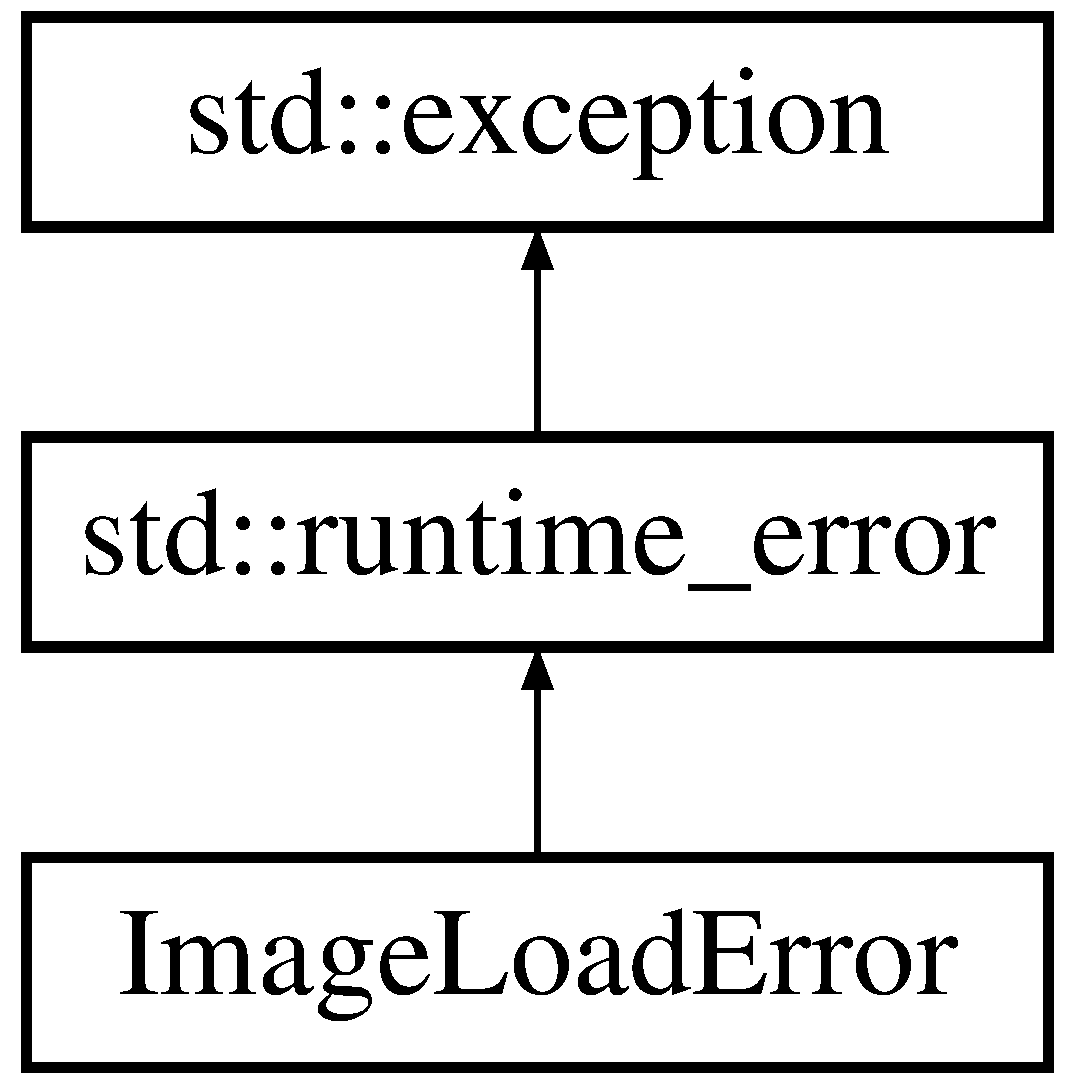
\includegraphics[height=3.000000cm]{classImageLoadError}
\end{center}
\end{figure}
\subsection*{Public Member Functions}
\begin{DoxyCompactItemize}
\item 
\hyperlink{classImageLoadError_a578b21971e45108555b175a9638b388d}{Image\+Load\+Error} (const string \&arg)
\begin{DoxyCompactList}\small\item\em Write what the function does here. \end{DoxyCompactList}\end{DoxyCompactItemize}


\subsection{Detailed Description}
Write what the function does here. 

\begin{DoxyReturn}{Returns}

\end{DoxyReturn}


Definition at line 18 of file image.\+h.



\subsection{Constructor \& Destructor Documentation}
\hypertarget{classImageLoadError_a578b21971e45108555b175a9638b388d}{\index{Image\+Load\+Error@{Image\+Load\+Error}!Image\+Load\+Error@{Image\+Load\+Error}}
\index{Image\+Load\+Error@{Image\+Load\+Error}!Image\+Load\+Error@{Image\+Load\+Error}}
\subsubsection[{Image\+Load\+Error}]{\setlength{\rightskip}{0pt plus 5cm}Image\+Load\+Error\+::\+Image\+Load\+Error (
\begin{DoxyParamCaption}
\item[{const string \&}]{arg}
\end{DoxyParamCaption}
)\hspace{0.3cm}{\ttfamily [inline]}, {\ttfamily [explicit]}}}\label{classImageLoadError_a578b21971e45108555b175a9638b388d}


Write what the function does here. 


\begin{DoxyParams}{Parameters}
{\em arg} & \\
\hline
\end{DoxyParams}
\begin{DoxyReturn}{Returns}

\end{DoxyReturn}


Definition at line 21 of file image.\+h.


\begin{DoxyCode}
30             : runtime\_error(arg)
31             \{
32             \}
\end{DoxyCode}


The documentation for this class was generated from the following file\+:\begin{DoxyCompactItemize}
\item 
image.\+h\end{DoxyCompactItemize}

\hypertarget{classImageNotLoaded}{\section{Image\+Not\+Loaded Class Reference}
\label{classImageNotLoaded}\index{Image\+Not\+Loaded@{Image\+Not\+Loaded}}
}
\subsection*{Public Member Functions}
\begin{DoxyCompactItemize}
\item 
\hypertarget{classImageNotLoaded_aad9b5b31181586b4b2f8bd2edb39a6c0}{{\bfseries Image\+Not\+Loaded} (const string \&s)}\label{classImageNotLoaded_aad9b5b31181586b4b2f8bd2edb39a6c0}

\end{DoxyCompactItemize}
\subsection*{Private Attributes}
\begin{DoxyCompactItemize}
\item 
\hypertarget{classImageNotLoaded_a28c737d646a7aab6e417ab9929ca1dc9}{string {\bfseries s}}\label{classImageNotLoaded_a28c737d646a7aab6e417ab9929ca1dc9}

\end{DoxyCompactItemize}
\subsection*{Friends}
\begin{DoxyCompactItemize}
\item 
\hypertarget{classImageNotLoaded_a8ebdf991e0e46c984ea27be29dc112fd}{ostream \& {\bfseries operator$<$$<$} (ostream \&, const \hyperlink{classImageNotLoaded}{Image\+Not\+Loaded} \&)}\label{classImageNotLoaded_a8ebdf991e0e46c984ea27be29dc112fd}

\end{DoxyCompactItemize}


\subsection{Detailed Description}


Definition at line 13 of file image.\+h.



The documentation for this class was generated from the following file\+:\begin{DoxyCompactItemize}
\item 
headers/image.\+h\end{DoxyCompactItemize}

\hypertarget{classImageNotSameException}{\section{Image\+Not\+Same\+Exception Class Reference}
\label{classImageNotSameException}\index{Image\+Not\+Same\+Exception@{Image\+Not\+Same\+Exception}}
}


Write what the function does here.  




{\ttfamily \#include $<$mesh.\+h$>$}

Inheritance diagram for Image\+Not\+Same\+Exception\+:\begin{figure}[H]
\begin{center}
\leavevmode
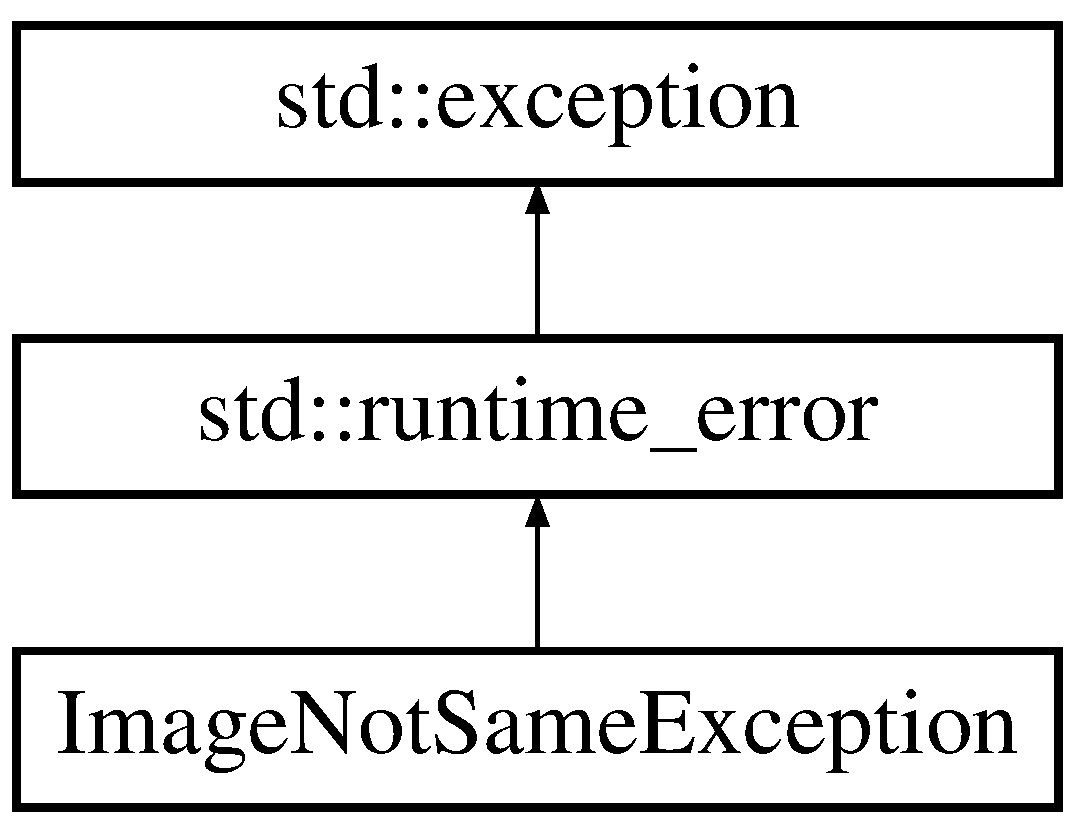
\includegraphics[height=3.000000cm]{classImageNotSameException}
\end{center}
\end{figure}


\subsection{Detailed Description}
Write what the function does here. 


\begin{DoxyRetVals}{Return values}
{\em (variable)} & (description of variable) \\
\hline
\end{DoxyRetVals}


Definition at line 216 of file mesh.\+h.



The documentation for this class was generated from the following file\+:\begin{DoxyCompactItemize}
\item 
mesh.\+h\end{DoxyCompactItemize}

\hypertarget{classinitializer}{\section{initializer Class Reference}
\label{classinitializer}\index{initializer@{initializer}}
}


Write what the function does here.  




{\ttfamily \#include $<$util.\+h$>$}

\subsection*{Public Member Functions}
\begin{DoxyCompactItemize}
\item 
\hypertarget{classinitializer_ad7eff8ec9662dda6c90a5eebbb5bb774}{{\bfseries initializer} (void($\ast$init\+Fn)(), void($\ast$finalize\+Fn)()=nullptr)}\label{classinitializer_ad7eff8ec9662dda6c90a5eebbb5bb774}

\item 
\hyperlink{classinitializer_a9ac296c0a8420f783af46a77792f4253}{$\sim$initializer} ()
\begin{DoxyCompactList}\small\item\em Write what the function does here. \end{DoxyCompactList}\end{DoxyCompactItemize}
\subsection*{Private Member Functions}
\begin{DoxyCompactItemize}
\item 
\hypertarget{classinitializer_a040920f2a1db4d0545d84c81ec6319d9}{{\bfseries initializer} (const \hyperlink{classinitializer}{initializer} \&rt)=delete}\label{classinitializer_a040920f2a1db4d0545d84c81ec6319d9}

\item 
\hypertarget{classinitializer_a622a590c3eeac8414877886cddb3c133}{void {\bfseries operator=} (const \hyperlink{classinitializer}{initializer} \&rt)=delete}\label{classinitializer_a622a590c3eeac8414877886cddb3c133}

\end{DoxyCompactItemize}
\subsection*{Private Attributes}
\begin{DoxyCompactItemize}
\item 
\hypertarget{classinitializer_abb0e43532e705e711cb64318defa0a4f}{void($\ast$ {\bfseries finalize\+Fn} )()}\label{classinitializer_abb0e43532e705e711cb64318defa0a4f}

\end{DoxyCompactItemize}


\subsection{Detailed Description}
Write what the function does here. 


\begin{DoxyRetVals}{Return values}
{\em (variable)} & (description of variable) \\
\hline
\end{DoxyRetVals}


Definition at line 114 of file util.\+h.



\subsection{Constructor \& Destructor Documentation}
\hypertarget{classinitializer_a9ac296c0a8420f783af46a77792f4253}{\index{initializer@{initializer}!````~initializer@{$\sim$initializer}}
\index{````~initializer@{$\sim$initializer}!initializer@{initializer}}
\subsubsection[{$\sim$initializer}]{\setlength{\rightskip}{0pt plus 5cm}initializer\+::$\sim$initializer (
\begin{DoxyParamCaption}
{}
\end{DoxyParamCaption}
)\hspace{0.3cm}{\ttfamily [inline]}}}\label{classinitializer_a9ac296c0a8420f783af46a77792f4253}


Write what the function does here. 


\begin{DoxyRetVals}{Return values}
{\em (variable)} & (description of variable) \\
\hline
\end{DoxyRetVals}


Definition at line 132 of file util.\+h.


\begin{DoxyCode}
133         \{
134 
135             \textcolor{keywordflow}{if}(finalizeFn)
136             \{
137                 finalizeFn();
138             \}
139         \}
\end{DoxyCode}


The documentation for this class was generated from the following file\+:\begin{DoxyCompactItemize}
\item 
util.\+h\end{DoxyCompactItemize}

\hypertarget{structinternal__state}{\section{internal\+\_\+state Struct Reference}
\label{structinternal__state}\index{internal\+\_\+state@{internal\+\_\+state}}
}
\subsection*{Public Attributes}
\begin{DoxyCompactItemize}
\item 
\hypertarget{structinternal__state_ab000a3e3c901dd063859521988ad7e52}{int {\bfseries dummy}}\label{structinternal__state_ab000a3e3c901dd063859521988ad7e52}

\end{DoxyCompactItemize}


\subsection{Detailed Description}


Definition at line 1346 of file zlib.\+h.



The documentation for this struct was generated from the following file\+:\begin{DoxyCompactItemize}
\item 
zlib.\+h\end{DoxyCompactItemize}

\hypertarget{classInvalidCorner}{\section{Invalid\+Corner Class Reference}
\label{classInvalidCorner}\index{Invalid\+Corner@{Invalid\+Corner}}
}


\subsection{Detailed Description}


Definition at line 60 of file node.\+h.



The documentation for this class was generated from the following file\+:\begin{DoxyCompactItemize}
\item 
headers/node.\+h\end{DoxyCompactItemize}

\hypertarget{classInvalidDataValueException}{\section{Invalid\+Data\+Value\+Exception Class Reference}
\label{classInvalidDataValueException}\index{Invalid\+Data\+Value\+Exception@{Invalid\+Data\+Value\+Exception}}
}


Write what the function does here.  




{\ttfamily \#include $<$stream.\+h$>$}

Inheritance diagram for Invalid\+Data\+Value\+Exception\+:\begin{figure}[H]
\begin{center}
\leavevmode
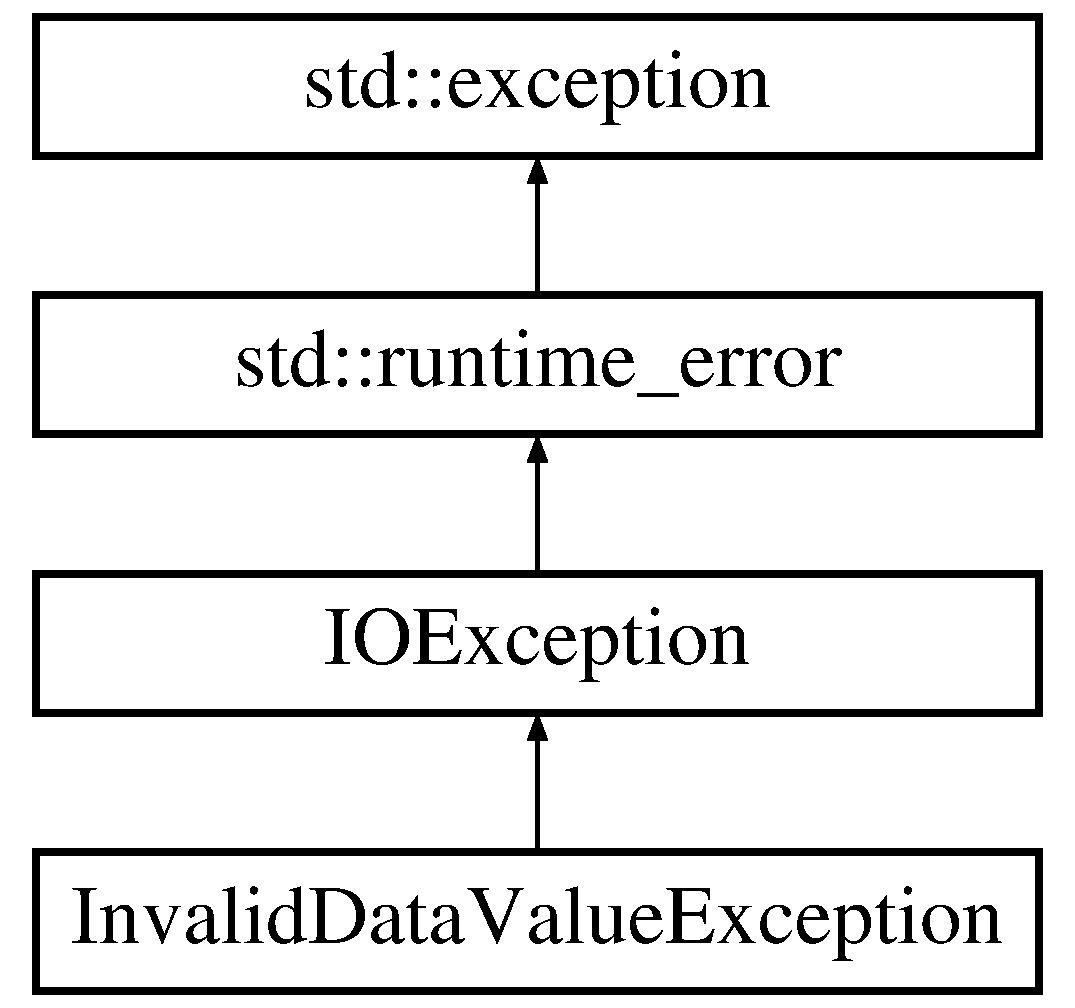
\includegraphics[height=4.000000cm]{classInvalidDataValueException}
\end{center}
\end{figure}
\subsection*{Public Member Functions}
\begin{DoxyCompactItemize}
\item 
\hyperlink{classInvalidDataValueException_a7f19492afda3de435899cce6c3b079ac}{Invalid\+Data\+Value\+Exception} (string msg)
\begin{DoxyCompactList}\small\item\em Write what the function does here. \end{DoxyCompactList}\end{DoxyCompactItemize}


\subsection{Detailed Description}
Write what the function does here. 

\begin{DoxyReturn}{Returns}

\end{DoxyReturn}


Definition at line 142 of file stream.\+h.



\subsection{Constructor \& Destructor Documentation}
\hypertarget{classInvalidDataValueException_a7f19492afda3de435899cce6c3b079ac}{\index{Invalid\+Data\+Value\+Exception@{Invalid\+Data\+Value\+Exception}!Invalid\+Data\+Value\+Exception@{Invalid\+Data\+Value\+Exception}}
\index{Invalid\+Data\+Value\+Exception@{Invalid\+Data\+Value\+Exception}!Invalid\+Data\+Value\+Exception@{Invalid\+Data\+Value\+Exception}}
\subsubsection[{Invalid\+Data\+Value\+Exception}]{\setlength{\rightskip}{0pt plus 5cm}Invalid\+Data\+Value\+Exception\+::\+Invalid\+Data\+Value\+Exception (
\begin{DoxyParamCaption}
\item[{string}]{msg}
\end{DoxyParamCaption}
)\hspace{0.3cm}{\ttfamily [inline]}, {\ttfamily [explicit]}}}\label{classInvalidDataValueException_a7f19492afda3de435899cce6c3b079ac}


Write what the function does here. 


\begin{DoxyParams}{Parameters}
{\em msg} & \\
\hline
\end{DoxyParams}
\begin{DoxyReturn}{Returns}

\end{DoxyReturn}


Definition at line 145 of file stream.\+h.


\begin{DoxyCode}
154             : \hyperlink{classIOException_a73fcf78b1b5820aa158680e896f0b983}{IOException}(msg)
155             \{
156             \}
\end{DoxyCode}


The documentation for this class was generated from the following file\+:\begin{DoxyCompactItemize}
\item 
stream.\+h\end{DoxyCompactItemize}

\hypertarget{classInvalidLine}{\section{Invalid\+Line Class Reference}
\label{classInvalidLine}\index{Invalid\+Line@{Invalid\+Line}}
}
\subsection*{Public Member Functions}
\begin{DoxyCompactItemize}
\item 
\hypertarget{classInvalidLine_ac92ceb5d32da96a53d288e3e8d1515f3}{{\bfseries Invalid\+Line} (const Line \&line)}\label{classInvalidLine_ac92ceb5d32da96a53d288e3e8d1515f3}

\end{DoxyCompactItemize}
\subsection*{Private Attributes}
\begin{DoxyCompactItemize}
\item 
\hypertarget{classInvalidLine_ab5317a753030b760c2b7047db84cfdc9}{Line {\bfseries line}}\label{classInvalidLine_ab5317a753030b760c2b7047db84cfdc9}

\end{DoxyCompactItemize}
\subsection*{Friends}
\begin{DoxyCompactItemize}
\item 
\hypertarget{classInvalidLine_a83dd5c7533a6e45a97ea781c6ec0d830}{ostream \& {\bfseries operator$<$$<$} (ostream \&, const \hyperlink{classInvalidLine}{Invalid\+Line} \&)}\label{classInvalidLine_a83dd5c7533a6e45a97ea781c6ec0d830}

\end{DoxyCompactItemize}


\subsection{Detailed Description}


Definition at line 49 of file node.\+h.



The documentation for this class was generated from the following file\+:\begin{DoxyCompactItemize}
\item 
headers/node.\+h\end{DoxyCompactItemize}

\hypertarget{classInvalidMiddle}{\section{Invalid\+Middle Class Reference}
\label{classInvalidMiddle}\index{Invalid\+Middle@{Invalid\+Middle}}
}
\subsection*{Public Member Functions}
\begin{DoxyCompactItemize}
\item 
\hypertarget{classInvalidMiddle_a9f95b57852f768294ff41b7b4d6504fc}{{\bfseries Invalid\+Middle} (int count, \hyperlink{structCoord}{Coord} middle)}\label{classInvalidMiddle_a9f95b57852f768294ff41b7b4d6504fc}

\end{DoxyCompactItemize}
\subsection*{Private Attributes}
\begin{DoxyCompactItemize}
\item 
\hypertarget{classInvalidMiddle_a0b3895584a08100d6993c06927a6aa47}{const int {\bfseries count}}\label{classInvalidMiddle_a0b3895584a08100d6993c06927a6aa47}

\item 
\hypertarget{classInvalidMiddle_a2b7ea531d435c0229ef911d8abe91022}{const \hyperlink{structCoord}{Coord} {\bfseries middle}}\label{classInvalidMiddle_a2b7ea531d435c0229ef911d8abe91022}

\end{DoxyCompactItemize}
\subsection*{Friends}
\begin{DoxyCompactItemize}
\item 
\hypertarget{classInvalidMiddle_a82776417931d3f6f2fdc00584390e12d}{ostream \& {\bfseries operator$<$$<$} (ostream \&os, const \hyperlink{classInvalidMiddle}{Invalid\+Middle} \&)}\label{classInvalidMiddle_a82776417931d3f6f2fdc00584390e12d}

\end{DoxyCompactItemize}


\subsection{Detailed Description}


Definition at line 36 of file game.\+h.



The documentation for this class was generated from the following file\+:\begin{DoxyCompactItemize}
\item 
headers/game.\+h\end{DoxyCompactItemize}

\hypertarget{classInvalidNode}{\section{Invalid\+Node Class Reference}
\label{classInvalidNode}\index{Invalid\+Node@{Invalid\+Node}}
}


\subsection{Detailed Description}


Definition at line 48 of file game.\+h.



The documentation for this class was generated from the following file\+:\begin{DoxyCompactItemize}
\item 
headers/game.\+h\end{DoxyCompactItemize}

\hypertarget{classIOException}{\section{I\+O\+Exception Class Reference}
\label{classIOException}\index{I\+O\+Exception@{I\+O\+Exception}}
}


Write what the function does here.  




{\ttfamily \#include $<$stream.\+h$>$}

Inheritance diagram for I\+O\+Exception\+:\begin{figure}[H]
\begin{center}
\leavevmode
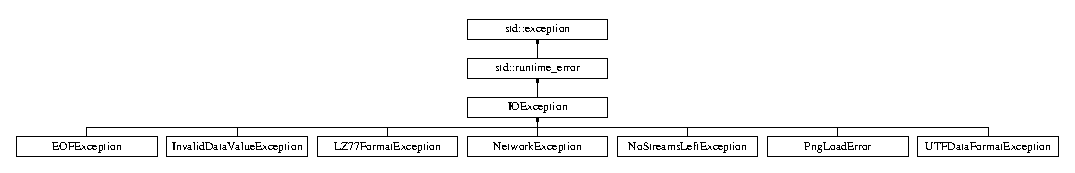
\includegraphics[height=1.871345cm]{classIOException}
\end{center}
\end{figure}
\subsection*{Public Member Functions}
\begin{DoxyCompactItemize}
\item 
\hyperlink{classIOException_a73fcf78b1b5820aa158680e896f0b983}{I\+O\+Exception} (const string \&msg)
\begin{DoxyCompactList}\small\item\em Write what the function does here. \end{DoxyCompactList}\item 
\hyperlink{classIOException_a286c271ca82812d1e7c12925acf33d14}{I\+O\+Exception} (exception $\ast$e, bool delete\+It=true)
\begin{DoxyCompactList}\small\item\em Write what the function does here. \end{DoxyCompactList}\item 
\hyperlink{classIOException_abf6ec1a6297e0558758ef144e9e36471}{I\+O\+Exception} (exception \&e, bool delete\+It=false)
\begin{DoxyCompactList}\small\item\em Write what the function does here. \end{DoxyCompactList}\end{DoxyCompactItemize}


\subsection{Detailed Description}
Write what the function does here. 

\begin{DoxyReturn}{Returns}

\end{DoxyReturn}


Definition at line 32 of file stream.\+h.



\subsection{Constructor \& Destructor Documentation}
\hypertarget{classIOException_a73fcf78b1b5820aa158680e896f0b983}{\index{I\+O\+Exception@{I\+O\+Exception}!I\+O\+Exception@{I\+O\+Exception}}
\index{I\+O\+Exception@{I\+O\+Exception}!I\+O\+Exception@{I\+O\+Exception}}
\subsubsection[{I\+O\+Exception}]{\setlength{\rightskip}{0pt plus 5cm}I\+O\+Exception\+::\+I\+O\+Exception (
\begin{DoxyParamCaption}
\item[{const string \&}]{msg}
\end{DoxyParamCaption}
)\hspace{0.3cm}{\ttfamily [inline]}, {\ttfamily [explicit]}}}\label{classIOException_a73fcf78b1b5820aa158680e896f0b983}


Write what the function does here. 


\begin{DoxyParams}{Parameters}
{\em msg} & \\
\hline
\end{DoxyParams}
\begin{DoxyReturn}{Returns}

\end{DoxyReturn}


Definition at line 35 of file stream.\+h.


\begin{DoxyCode}
44             : runtime\_error(msg)
45             \{
46             \}
\end{DoxyCode}
\hypertarget{classIOException_a286c271ca82812d1e7c12925acf33d14}{\index{I\+O\+Exception@{I\+O\+Exception}!I\+O\+Exception@{I\+O\+Exception}}
\index{I\+O\+Exception@{I\+O\+Exception}!I\+O\+Exception@{I\+O\+Exception}}
\subsubsection[{I\+O\+Exception}]{\setlength{\rightskip}{0pt plus 5cm}I\+O\+Exception\+::\+I\+O\+Exception (
\begin{DoxyParamCaption}
\item[{exception $\ast$}]{e, }
\item[{bool}]{delete\+It = {\ttfamily true}}
\end{DoxyParamCaption}
)\hspace{0.3cm}{\ttfamily [inline]}, {\ttfamily [explicit]}}}\label{classIOException_a286c271ca82812d1e7c12925acf33d14}


Write what the function does here. 


\begin{DoxyParams}{Parameters}
{\em e} & \\
\hline
{\em nullptr} & \\
\hline
\end{DoxyParams}
\begin{DoxyReturn}{Returns}

\end{DoxyReturn}


Definition at line 47 of file stream.\+h.


\begin{DoxyCode}
57             : runtime\_error((dynamic\_cast<IOException *>(e) == \textcolor{keyword}{nullptr}) ? \textcolor{keywordtype}{string}(\textcolor{stringliteral}{"IO Error : "}) + e->what()
       : string(e->what()))
58             \{
59                 \textcolor{keywordflow}{if}(deleteIt)
60                     \textcolor{keyword}{delete} e;
61             \}
\end{DoxyCode}
\hypertarget{classIOException_abf6ec1a6297e0558758ef144e9e36471}{\index{I\+O\+Exception@{I\+O\+Exception}!I\+O\+Exception@{I\+O\+Exception}}
\index{I\+O\+Exception@{I\+O\+Exception}!I\+O\+Exception@{I\+O\+Exception}}
\subsubsection[{I\+O\+Exception}]{\setlength{\rightskip}{0pt plus 5cm}I\+O\+Exception\+::\+I\+O\+Exception (
\begin{DoxyParamCaption}
\item[{exception \&}]{e, }
\item[{bool}]{delete\+It = {\ttfamily false}}
\end{DoxyParamCaption}
)\hspace{0.3cm}{\ttfamily [inline]}, {\ttfamily [explicit]}}}\label{classIOException_abf6ec1a6297e0558758ef144e9e36471}


Write what the function does here. 


\begin{DoxyParams}{Parameters}
{\em e} & \\
\hline
{\em delete\+It} & \\
\hline
\end{DoxyParams}
\begin{DoxyReturn}{Returns}

\end{DoxyReturn}


Definition at line 62 of file stream.\+h.


\begin{DoxyCode}
72             : \hyperlink{classIOException_a73fcf78b1b5820aa158680e896f0b983}{IOException}(&e, deleteIt)
73             \{
74             \}
\end{DoxyCode}


The documentation for this class was generated from the following file\+:\begin{DoxyCompactItemize}
\item 
stream.\+h\end{DoxyCompactItemize}

\hypertarget{classcircularDeque_1_1iterator}{\section{circular\+Deque$<$ T, array\+Size $>$\+:\+:iterator Class Reference}
\label{classcircularDeque_1_1iterator}\index{circular\+Deque$<$ T, array\+Size $>$\+::iterator@{circular\+Deque$<$ T, array\+Size $>$\+::iterator}}
}


Write what the function does here.  




{\ttfamily \#include $<$util.\+h$>$}

Inheritance diagram for circular\+Deque$<$ T, array\+Size $>$\+:\+:iterator\+:\begin{figure}[H]
\begin{center}
\leavevmode
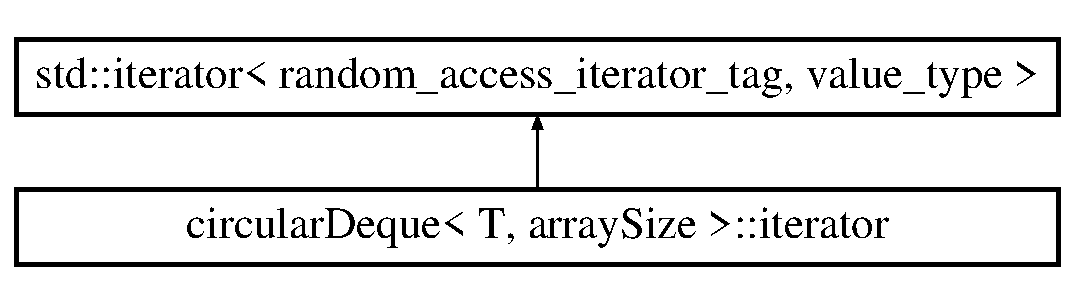
\includegraphics[height=2.000000cm]{classcircularDeque_1_1iterator}
\end{center}
\end{figure}
\subsection*{Public Member Functions}
\begin{DoxyCompactItemize}
\item 
\hyperlink{classcircularDeque_1_1iterator}{iterator} \& \hyperlink{classcircularDeque_1_1iterator_adab937de09a3bebfc08b5bdc13ab55c5}{operator+=} (difference\+\_\+type n)
\begin{DoxyCompactList}\small\item\em Write what the function does here. \end{DoxyCompactList}\item 
\hyperlink{classcircularDeque_1_1iterator}{iterator} \& \hyperlink{classcircularDeque_1_1iterator_ae465975e1491a6cb84a890ae8a762eea}{operator-\/=} (difference\+\_\+type n)
\begin{DoxyCompactList}\small\item\em Write what the function does here. \end{DoxyCompactList}\item 
\hypertarget{classcircularDeque_1_1iterator_aec2396234b3a5d2d1449c5e83619917d}{difference\+\_\+type {\bfseries operator-\/} (const \hyperlink{classcircularDeque_1_1iterator}{iterator} \&r) const }\label{classcircularDeque_1_1iterator_aec2396234b3a5d2d1449c5e83619917d}

\item 
T \& \hyperlink{classcircularDeque_1_1iterator_a21a49d0edbe140af0ed4b8ef1734f439}{operator\mbox{[}$\,$\mbox{]}} (difference\+\_\+type n) const 
\begin{DoxyCompactList}\small\item\em Write what the function does here. \end{DoxyCompactList}\item 
T \& \hyperlink{classcircularDeque_1_1iterator_af85542e8915ee6e3cfd958221a789a52}{operator$\ast$} () const 
\begin{DoxyCompactList}\small\item\em Write what the function does here. \end{DoxyCompactList}\item 
T $\ast$ \hyperlink{classcircularDeque_1_1iterator_ad2d0ef1f228b917212a6d7a84fa6c938}{operator-\/$>$} () const 
\begin{DoxyCompactList}\small\item\em Write what the function does here. \end{DoxyCompactList}\item 
const \hyperlink{classcircularDeque_1_1iterator}{iterator} \& \hyperlink{classcircularDeque_1_1iterator_ad85f34565b4f79c0e9c758e75594d04c}{operator-\/-\/} ()
\begin{DoxyCompactList}\small\item\em Write what the function does here. \end{DoxyCompactList}\item 
\hyperlink{classcircularDeque_1_1iterator}{iterator} \hyperlink{classcircularDeque_1_1iterator_a601345dba4440eaa80c372d8d6b1fd72}{operator-\/-\/} (int)
\begin{DoxyCompactList}\small\item\em Write what the function does here. \end{DoxyCompactList}\item 
const \hyperlink{classcircularDeque_1_1iterator}{iterator} \& \hyperlink{classcircularDeque_1_1iterator_a54abaeb1841ae8384be053ca64d75e03}{operator++} ()
\begin{DoxyCompactList}\small\item\em Write what the function does here. \end{DoxyCompactList}\item 
\hyperlink{classcircularDeque_1_1iterator}{iterator} \hyperlink{classcircularDeque_1_1iterator_a770427aacdfea8b4f452bde2a38fe622}{operator++} (int)
\begin{DoxyCompactList}\small\item\em Write what the function does here. \end{DoxyCompactList}\end{DoxyCompactItemize}
\subsection*{Private Member Functions}
\begin{DoxyCompactItemize}
\item 
\hypertarget{classcircularDeque_1_1iterator_a137521582461a1f2fee4f600173ba789}{{\bfseries iterator} (\hyperlink{classcircularDeque}{circular\+Deque} $\ast$container, size\+\_\+t index)}\label{classcircularDeque_1_1iterator_a137521582461a1f2fee4f600173ba789}

\end{DoxyCompactItemize}
\subsection*{Private Attributes}
\begin{DoxyCompactItemize}
\item 
\hypertarget{classcircularDeque_1_1iterator_a6df5ff5d1f6afe89b6e7c070c07b8d1c}{\hyperlink{classcircularDeque}{circular\+Deque} $\ast$ {\bfseries container}}\label{classcircularDeque_1_1iterator_a6df5ff5d1f6afe89b6e7c070c07b8d1c}

\item 
\hypertarget{classcircularDeque_1_1iterator_a099c533da98b34ee5415675fd905dc36}{size\+\_\+t {\bfseries index}}\label{classcircularDeque_1_1iterator_a099c533da98b34ee5415675fd905dc36}

\end{DoxyCompactItemize}
\subsection*{Friends}
\begin{DoxyCompactItemize}
\item 
\hypertarget{classcircularDeque_1_1iterator_aa63d8b47e75b076d05ec6aa14e29109b}{class {\bfseries circular\+Deque}}\label{classcircularDeque_1_1iterator_aa63d8b47e75b076d05ec6aa14e29109b}

\item 
\hypertarget{classcircularDeque_1_1iterator_ac220ce1c155db1ac44146c12d178056f}{class {\bfseries const\+\_\+iterator}}\label{classcircularDeque_1_1iterator_ac220ce1c155db1ac44146c12d178056f}

\item 
\hyperlink{classcircularDeque_1_1iterator}{iterator} \hyperlink{classcircularDeque_1_1iterator_ac16e910c895e60a596b80b7c86fc1515}{operator+} (difference\+\_\+type n, \hyperlink{classcircularDeque_1_1iterator}{iterator} i)
\begin{DoxyCompactList}\small\item\em Write what the function does here. \end{DoxyCompactList}\item 
\hyperlink{classcircularDeque_1_1iterator}{iterator} \hyperlink{classcircularDeque_1_1iterator_ac75e470ef6da99b63e93e64a6564b50c}{operator+} (\hyperlink{classcircularDeque_1_1iterator}{iterator} i, difference\+\_\+type n)
\begin{DoxyCompactList}\small\item\em Write what the function does here. \end{DoxyCompactList}\item 
\hyperlink{classcircularDeque_1_1iterator}{iterator} \hyperlink{classcircularDeque_1_1iterator_a909c554e380a6de09d132abaf5868326}{operator-\/} (\hyperlink{classcircularDeque_1_1iterator}{iterator} i, difference\+\_\+type n)
\begin{DoxyCompactList}\small\item\em Write what the function does here. \end{DoxyCompactList}\item 
bool \hyperlink{classcircularDeque_1_1iterator_a507249f95531109aebe1ea4324c03c63}{operator==} (const \hyperlink{classcircularDeque_1_1iterator}{iterator} \&l, const \hyperlink{classcircularDeque_1_1iterator}{iterator} \&r)
\begin{DoxyCompactList}\small\item\em Write what the function does here. \end{DoxyCompactList}\item 
bool \hyperlink{classcircularDeque_1_1iterator_aef216496a914d7abfe28c6ea6ec433ad}{operator!=} (const \hyperlink{classcircularDeque_1_1iterator}{iterator} \&l, const \hyperlink{classcircularDeque_1_1iterator}{iterator} \&r)
\begin{DoxyCompactList}\small\item\em Write what the function does here. \end{DoxyCompactList}\item 
bool \hyperlink{classcircularDeque_1_1iterator_a90290eb7089c69859452250df85a3756}{operator$>$} (const \hyperlink{classcircularDeque_1_1iterator}{iterator} \&l, const \hyperlink{classcircularDeque_1_1iterator}{iterator} \&r)
\begin{DoxyCompactList}\small\item\em Write what the function does here. \end{DoxyCompactList}\item 
bool \hyperlink{classcircularDeque_1_1iterator_ab23d72047381dab9b9888b88d4662d15}{operator$>$=} (const \hyperlink{classcircularDeque_1_1iterator}{iterator} \&l, const \hyperlink{classcircularDeque_1_1iterator}{iterator} \&r)
\begin{DoxyCompactList}\small\item\em Write what the function does here. \end{DoxyCompactList}\item 
bool \hyperlink{classcircularDeque_1_1iterator_abaee5f90fefec343d2a1bc4a7ffaa1d0}{operator$<$} (const \hyperlink{classcircularDeque_1_1iterator}{iterator} \&l, const \hyperlink{classcircularDeque_1_1iterator}{iterator} \&r)
\begin{DoxyCompactList}\small\item\em Write what the function does here. \end{DoxyCompactList}\item 
bool \hyperlink{classcircularDeque_1_1iterator_a48af46c9be3de4731ed1e9fc1aaf1421}{operator$<$=} (const \hyperlink{classcircularDeque_1_1iterator}{iterator} \&l, const \hyperlink{classcircularDeque_1_1iterator}{iterator} \&r)
\begin{DoxyCompactList}\small\item\em Write what the function does here. \end{DoxyCompactList}\end{DoxyCompactItemize}


\subsection{Detailed Description}
\subsubsection*{template$<$typename T, size\+\_\+t array\+Size$>$class circular\+Deque$<$ T, array\+Size $>$\+::iterator}

Write what the function does here. 


\begin{DoxyParams}{Parameters}
{\em random\+\_\+access\+\_\+iterator\+\_\+tag} & \\
\hline
\end{DoxyParams}

\begin{DoxyRetVals}{Return values}
{\em (variable)} & (description of variable) \\
\hline
\end{DoxyRetVals}


Definition at line 264 of file util.\+h.



\subsection{Member Function Documentation}
\hypertarget{classcircularDeque_1_1iterator_af85542e8915ee6e3cfd958221a789a52}{\index{circular\+Deque\+::iterator@{circular\+Deque\+::iterator}!operator$\ast$@{operator$\ast$}}
\index{operator$\ast$@{operator$\ast$}!circular\+Deque\+::iterator@{circular\+Deque\+::iterator}}
\subsubsection[{operator$\ast$}]{\setlength{\rightskip}{0pt plus 5cm}template$<$typename T, size\+\_\+t array\+Size$>$ T\& {\bf circular\+Deque}$<$ T, array\+Size $>$\+::iterator\+::operator$\ast$ (
\begin{DoxyParamCaption}
{}
\end{DoxyParamCaption}
) const\hspace{0.3cm}{\ttfamily [inline]}}}\label{classcircularDeque_1_1iterator_af85542e8915ee6e3cfd958221a789a52}


Write what the function does here. 


\begin{DoxyRetVals}{Return values}
{\em (variable)} & (description of variable) \\
\hline
\end{DoxyRetVals}


Definition at line 401 of file util.\+h.


\begin{DoxyCode}
402         \{
403             \textcolor{keywordflow}{return} container->array[index];
404         \}
\end{DoxyCode}
\hypertarget{classcircularDeque_1_1iterator_a54abaeb1841ae8384be053ca64d75e03}{\index{circular\+Deque\+::iterator@{circular\+Deque\+::iterator}!operator++@{operator++}}
\index{operator++@{operator++}!circular\+Deque\+::iterator@{circular\+Deque\+::iterator}}
\subsubsection[{operator++}]{\setlength{\rightskip}{0pt plus 5cm}template$<$typename T, size\+\_\+t array\+Size$>$ const {\bf iterator}\& {\bf circular\+Deque}$<$ T, array\+Size $>$\+::iterator\+::operator++ (
\begin{DoxyParamCaption}
{}
\end{DoxyParamCaption}
)\hspace{0.3cm}{\ttfamily [inline]}}}\label{classcircularDeque_1_1iterator_a54abaeb1841ae8384be053ca64d75e03}


Write what the function does here. 


\begin{DoxyRetVals}{Return values}
{\em (variable)} & (description of variable) \\
\hline
\end{DoxyRetVals}


Definition at line 464 of file util.\+h.


\begin{DoxyCode}
465         \{
466 
467             \textcolor{keywordflow}{if}(index >= arraySize - 1)
468             \{
469                 index = 0;
470             \}
471 
472             \textcolor{keywordflow}{else}
473             \{
474                 index++;
475             \}
476             \textcolor{keywordflow}{return} *\textcolor{keyword}{this};
477         \}
\end{DoxyCode}
\hypertarget{classcircularDeque_1_1iterator_a770427aacdfea8b4f452bde2a38fe622}{\index{circular\+Deque\+::iterator@{circular\+Deque\+::iterator}!operator++@{operator++}}
\index{operator++@{operator++}!circular\+Deque\+::iterator@{circular\+Deque\+::iterator}}
\subsubsection[{operator++}]{\setlength{\rightskip}{0pt plus 5cm}template$<$typename T, size\+\_\+t array\+Size$>$ {\bf iterator} {\bf circular\+Deque}$<$ T, array\+Size $>$\+::iterator\+::operator++ (
\begin{DoxyParamCaption}
\item[{int}]{}
\end{DoxyParamCaption}
)\hspace{0.3cm}{\ttfamily [inline]}}}\label{classcircularDeque_1_1iterator_a770427aacdfea8b4f452bde2a38fe622}


Write what the function does here. 


\begin{DoxyParams}{Parameters}
{\em int} & \\
\hline
\end{DoxyParams}

\begin{DoxyRetVals}{Return values}
{\em (variable)} & (description of variable) \\
\hline
\end{DoxyRetVals}


Definition at line 486 of file util.\+h.


\begin{DoxyCode}
487         \{
488             iterator retval = *\textcolor{keyword}{this};
489 
490             \textcolor{keywordflow}{if}(index >= arraySize - 1)
491             \{
492                 index = 0;
493             \}
494 
495             \textcolor{keywordflow}{else}
496             \{
497                 index++;
498             \}
499             \textcolor{keywordflow}{return} retval;
500         \}
\end{DoxyCode}
\hypertarget{classcircularDeque_1_1iterator_adab937de09a3bebfc08b5bdc13ab55c5}{\index{circular\+Deque\+::iterator@{circular\+Deque\+::iterator}!operator+=@{operator+=}}
\index{operator+=@{operator+=}!circular\+Deque\+::iterator@{circular\+Deque\+::iterator}}
\subsubsection[{operator+=}]{\setlength{\rightskip}{0pt plus 5cm}template$<$typename T, size\+\_\+t array\+Size$>$ {\bf iterator}\& {\bf circular\+Deque}$<$ T, array\+Size $>$\+::iterator\+::operator+= (
\begin{DoxyParamCaption}
\item[{difference\+\_\+type}]{n}
\end{DoxyParamCaption}
)\hspace{0.3cm}{\ttfamily [inline]}}}\label{classcircularDeque_1_1iterator_adab937de09a3bebfc08b5bdc13ab55c5}


Write what the function does here. 


\begin{DoxyParams}{Parameters}
{\em n} & \\
\hline
\end{DoxyParams}

\begin{DoxyRetVals}{Return values}
{\em (variable)} & (description of variable) \\
\hline
\end{DoxyRetVals}


Definition at line 288 of file util.\+h.


\begin{DoxyCode}
289         \{
290 
291             \textcolor{keywordflow}{if}(-n > (difference\_type)index)
292             \{
293                 n = n % arraySize + arraySize;
294             \}
295             index += n;
296             index %= arraySize;
297 
298             \textcolor{keywordflow}{if}(index < 0)
299             \{
300                 index += arraySize;
301             \}
302             \textcolor{keywordflow}{return} *\textcolor{keyword}{this};
303         \}
\end{DoxyCode}
\hypertarget{classcircularDeque_1_1iterator_ad85f34565b4f79c0e9c758e75594d04c}{\index{circular\+Deque\+::iterator@{circular\+Deque\+::iterator}!operator-\/-\/@{operator-\/-\/}}
\index{operator-\/-\/@{operator-\/-\/}!circular\+Deque\+::iterator@{circular\+Deque\+::iterator}}
\subsubsection[{operator-\/-\/}]{\setlength{\rightskip}{0pt plus 5cm}template$<$typename T, size\+\_\+t array\+Size$>$ const {\bf iterator}\& {\bf circular\+Deque}$<$ T, array\+Size $>$\+::iterator\+::operator-\/-\/ (
\begin{DoxyParamCaption}
{}
\end{DoxyParamCaption}
)\hspace{0.3cm}{\ttfamily [inline]}}}\label{classcircularDeque_1_1iterator_ad85f34565b4f79c0e9c758e75594d04c}


Write what the function does here. 


\begin{DoxyRetVals}{Return values}
{\em (variable)} & (description of variable) \\
\hline
\end{DoxyRetVals}


Definition at line 421 of file util.\+h.


\begin{DoxyCode}
422         \{
423 
424             \textcolor{keywordflow}{if}(index == 0)
425             \{
426                 index = arraySize - 1;
427             \}
428 
429             \textcolor{keywordflow}{else}
430             \{
431                 index--;
432             \}
433             \textcolor{keywordflow}{return} *\textcolor{keyword}{this};
434         \}
\end{DoxyCode}
\hypertarget{classcircularDeque_1_1iterator_a601345dba4440eaa80c372d8d6b1fd72}{\index{circular\+Deque\+::iterator@{circular\+Deque\+::iterator}!operator-\/-\/@{operator-\/-\/}}
\index{operator-\/-\/@{operator-\/-\/}!circular\+Deque\+::iterator@{circular\+Deque\+::iterator}}
\subsubsection[{operator-\/-\/}]{\setlength{\rightskip}{0pt plus 5cm}template$<$typename T, size\+\_\+t array\+Size$>$ {\bf iterator} {\bf circular\+Deque}$<$ T, array\+Size $>$\+::iterator\+::operator-\/-\/ (
\begin{DoxyParamCaption}
\item[{int}]{}
\end{DoxyParamCaption}
)\hspace{0.3cm}{\ttfamily [inline]}}}\label{classcircularDeque_1_1iterator_a601345dba4440eaa80c372d8d6b1fd72}


Write what the function does here. 


\begin{DoxyParams}{Parameters}
{\em int} & \\
\hline
\end{DoxyParams}

\begin{DoxyRetVals}{Return values}
{\em (variable)} & (description of variable) \\
\hline
\end{DoxyRetVals}


Definition at line 443 of file util.\+h.


\begin{DoxyCode}
444         \{
445             iterator retval = *\textcolor{keyword}{this};
446 
447             \textcolor{keywordflow}{if}(index == 0)
448             \{
449                 index = arraySize - 1;
450             \}
451 
452             \textcolor{keywordflow}{else}
453             \{
454                 index--;
455             \}
456             \textcolor{keywordflow}{return} retval;
457         \}
\end{DoxyCode}
\hypertarget{classcircularDeque_1_1iterator_ae465975e1491a6cb84a890ae8a762eea}{\index{circular\+Deque\+::iterator@{circular\+Deque\+::iterator}!operator-\/=@{operator-\/=}}
\index{operator-\/=@{operator-\/=}!circular\+Deque\+::iterator@{circular\+Deque\+::iterator}}
\subsubsection[{operator-\/=}]{\setlength{\rightskip}{0pt plus 5cm}template$<$typename T, size\+\_\+t array\+Size$>$ {\bf iterator}\& {\bf circular\+Deque}$<$ T, array\+Size $>$\+::iterator\+::operator-\/= (
\begin{DoxyParamCaption}
\item[{difference\+\_\+type}]{n}
\end{DoxyParamCaption}
)\hspace{0.3cm}{\ttfamily [inline]}}}\label{classcircularDeque_1_1iterator_ae465975e1491a6cb84a890ae8a762eea}


Write what the function does here. 


\begin{DoxyParams}{Parameters}
{\em n} & \\
\hline
\end{DoxyParams}

\begin{DoxyRetVals}{Return values}
{\em (variable)} & (description of variable) \\
\hline
\end{DoxyRetVals}


Definition at line 312 of file util.\+h.


\begin{DoxyCode}
313         \{
314             \textcolor{keywordflow}{return} *\textcolor{keyword}{this} += -n;
315         \}
\end{DoxyCode}
\hypertarget{classcircularDeque_1_1iterator_ad2d0ef1f228b917212a6d7a84fa6c938}{\index{circular\+Deque\+::iterator@{circular\+Deque\+::iterator}!operator-\/$>$@{operator-\/$>$}}
\index{operator-\/$>$@{operator-\/$>$}!circular\+Deque\+::iterator@{circular\+Deque\+::iterator}}
\subsubsection[{operator-\/$>$}]{\setlength{\rightskip}{0pt plus 5cm}template$<$typename T, size\+\_\+t array\+Size$>$ T$\ast$ {\bf circular\+Deque}$<$ T, array\+Size $>$\+::iterator\+::operator-\/$>$ (
\begin{DoxyParamCaption}
{}
\end{DoxyParamCaption}
) const\hspace{0.3cm}{\ttfamily [inline]}}}\label{classcircularDeque_1_1iterator_ad2d0ef1f228b917212a6d7a84fa6c938}


Write what the function does here. 


\begin{DoxyRetVals}{Return values}
{\em (variable)} & (description of variable) \\
\hline
\end{DoxyRetVals}


Definition at line 411 of file util.\+h.


\begin{DoxyCode}
412         \{
413             \textcolor{keywordflow}{return} container->array + index;
414         \}
\end{DoxyCode}
\hypertarget{classcircularDeque_1_1iterator_a21a49d0edbe140af0ed4b8ef1734f439}{\index{circular\+Deque\+::iterator@{circular\+Deque\+::iterator}!operator\mbox{[}$\,$\mbox{]}@{operator[]}}
\index{operator\mbox{[}$\,$\mbox{]}@{operator[]}!circular\+Deque\+::iterator@{circular\+Deque\+::iterator}}
\subsubsection[{operator[]}]{\setlength{\rightskip}{0pt plus 5cm}template$<$typename T, size\+\_\+t array\+Size$>$ T\& {\bf circular\+Deque}$<$ T, array\+Size $>$\+::iterator\+::operator\mbox{[}$\,$\mbox{]} (
\begin{DoxyParamCaption}
\item[{difference\+\_\+type}]{n}
\end{DoxyParamCaption}
) const\hspace{0.3cm}{\ttfamily [inline]}}}\label{classcircularDeque_1_1iterator_a21a49d0edbe140af0ed4b8ef1734f439}


Write what the function does here. 


\begin{DoxyParams}{Parameters}
{\em n} & \\
\hline
\end{DoxyParams}

\begin{DoxyRetVals}{Return values}
{\em (variable)} & (description of variable) \\
\hline
\end{DoxyRetVals}


Definition at line 391 of file util.\+h.


\begin{DoxyCode}
392         \{
393             \textcolor{keywordflow}{return} *(*\textcolor{keyword}{this} + n);
394         \}
\end{DoxyCode}


\subsection{Friends And Related Function Documentation}
\hypertarget{classcircularDeque_1_1iterator_aef216496a914d7abfe28c6ea6ec433ad}{\index{circular\+Deque\+::iterator@{circular\+Deque\+::iterator}!operator"!=@{operator"!=}}
\index{operator"!=@{operator"!=}!circular\+Deque\+::iterator@{circular\+Deque\+::iterator}}
\subsubsection[{operator"!=}]{\setlength{\rightskip}{0pt plus 5cm}template$<$typename T, size\+\_\+t array\+Size$>$ bool operator!= (
\begin{DoxyParamCaption}
\item[{const {\bf iterator} \&}]{l, }
\item[{const {\bf iterator} \&}]{r}
\end{DoxyParamCaption}
)\hspace{0.3cm}{\ttfamily [friend]}}}\label{classcircularDeque_1_1iterator_aef216496a914d7abfe28c6ea6ec433ad}


Write what the function does here. 


\begin{DoxyParams}{Parameters}
{\em l} & \\
\hline
{\em r} & \\
\hline
\end{DoxyParams}

\begin{DoxyRetVals}{Return values}
{\em (variable)} & (description of variable) \\
\hline
\end{DoxyRetVals}


Definition at line 523 of file util.\+h.


\begin{DoxyCode}
524         \{
525             \textcolor{keywordflow}{return} l.index != r.index;
526         \}
\end{DoxyCode}
\hypertarget{classcircularDeque_1_1iterator_ac16e910c895e60a596b80b7c86fc1515}{\index{circular\+Deque\+::iterator@{circular\+Deque\+::iterator}!operator+@{operator+}}
\index{operator+@{operator+}!circular\+Deque\+::iterator@{circular\+Deque\+::iterator}}
\subsubsection[{operator+}]{\setlength{\rightskip}{0pt plus 5cm}template$<$typename T, size\+\_\+t array\+Size$>$ {\bf iterator} operator+ (
\begin{DoxyParamCaption}
\item[{difference\+\_\+type}]{n, }
\item[{{\bf iterator}}]{i}
\end{DoxyParamCaption}
)\hspace{0.3cm}{\ttfamily [friend]}}}\label{classcircularDeque_1_1iterator_ac16e910c895e60a596b80b7c86fc1515}


Write what the function does here. 


\begin{DoxyParams}{Parameters}
{\em n} & \\
\hline
{\em i} & \\
\hline
\end{DoxyParams}

\begin{DoxyRetVals}{Return values}
{\em (variable)} & (description of variable) \\
\hline
\end{DoxyRetVals}


Definition at line 325 of file util.\+h.


\begin{DoxyCode}
326         \{
327             \textcolor{keywordflow}{return} i += n;
328         \}
\end{DoxyCode}
\hypertarget{classcircularDeque_1_1iterator_ac75e470ef6da99b63e93e64a6564b50c}{\index{circular\+Deque\+::iterator@{circular\+Deque\+::iterator}!operator+@{operator+}}
\index{operator+@{operator+}!circular\+Deque\+::iterator@{circular\+Deque\+::iterator}}
\subsubsection[{operator+}]{\setlength{\rightskip}{0pt plus 5cm}template$<$typename T, size\+\_\+t array\+Size$>$ {\bf iterator} operator+ (
\begin{DoxyParamCaption}
\item[{{\bf iterator}}]{i, }
\item[{difference\+\_\+type}]{n}
\end{DoxyParamCaption}
)\hspace{0.3cm}{\ttfamily [friend]}}}\label{classcircularDeque_1_1iterator_ac75e470ef6da99b63e93e64a6564b50c}


Write what the function does here. 


\begin{DoxyParams}{Parameters}
{\em i} & \\
\hline
{\em n} & \\
\hline
\end{DoxyParams}

\begin{DoxyRetVals}{Return values}
{\em (variable)} & (description of variable) \\
\hline
\end{DoxyRetVals}


Definition at line 338 of file util.\+h.


\begin{DoxyCode}
339         \{
340             \textcolor{keywordflow}{return} i += n;
341         \}
\end{DoxyCode}
\hypertarget{classcircularDeque_1_1iterator_a909c554e380a6de09d132abaf5868326}{\index{circular\+Deque\+::iterator@{circular\+Deque\+::iterator}!operator-\/@{operator-\/}}
\index{operator-\/@{operator-\/}!circular\+Deque\+::iterator@{circular\+Deque\+::iterator}}
\subsubsection[{operator-\/}]{\setlength{\rightskip}{0pt plus 5cm}template$<$typename T, size\+\_\+t array\+Size$>$ {\bf iterator} operator-\/ (
\begin{DoxyParamCaption}
\item[{{\bf iterator}}]{i, }
\item[{difference\+\_\+type}]{n}
\end{DoxyParamCaption}
)\hspace{0.3cm}{\ttfamily [friend]}}}\label{classcircularDeque_1_1iterator_a909c554e380a6de09d132abaf5868326}


Write what the function does here. 


\begin{DoxyParams}{Parameters}
{\em i} & \\
\hline
{\em n} & \\
\hline
\end{DoxyParams}

\begin{DoxyRetVals}{Return values}
{\em (variable)} & (description of variable) \\
\hline
\end{DoxyRetVals}


Definition at line 351 of file util.\+h.


\begin{DoxyCode}
352         \{
353             \textcolor{keywordflow}{return} i -= n;
354         \}
\end{DoxyCode}
\hypertarget{classcircularDeque_1_1iterator_abaee5f90fefec343d2a1bc4a7ffaa1d0}{\index{circular\+Deque\+::iterator@{circular\+Deque\+::iterator}!operator$<$@{operator$<$}}
\index{operator$<$@{operator$<$}!circular\+Deque\+::iterator@{circular\+Deque\+::iterator}}
\subsubsection[{operator$<$}]{\setlength{\rightskip}{0pt plus 5cm}template$<$typename T, size\+\_\+t array\+Size$>$ bool operator$<$ (
\begin{DoxyParamCaption}
\item[{const {\bf iterator} \&}]{l, }
\item[{const {\bf iterator} \&}]{r}
\end{DoxyParamCaption}
)\hspace{0.3cm}{\ttfamily [friend]}}}\label{classcircularDeque_1_1iterator_abaee5f90fefec343d2a1bc4a7ffaa1d0}


Write what the function does here. 


\begin{DoxyParams}{Parameters}
{\em l} & \\
\hline
{\em r} & \\
\hline
\end{DoxyParams}

\begin{DoxyRetVals}{Return values}
{\em (variable)} & (description of variable) \\
\hline
\end{DoxyRetVals}


Definition at line 562 of file util.\+h.


\begin{DoxyCode}
563         \{
564             \textcolor{keywordflow}{return} (l - r) < 0;
565         \}
\end{DoxyCode}
\hypertarget{classcircularDeque_1_1iterator_a48af46c9be3de4731ed1e9fc1aaf1421}{\index{circular\+Deque\+::iterator@{circular\+Deque\+::iterator}!operator$<$=@{operator$<$=}}
\index{operator$<$=@{operator$<$=}!circular\+Deque\+::iterator@{circular\+Deque\+::iterator}}
\subsubsection[{operator$<$=}]{\setlength{\rightskip}{0pt plus 5cm}template$<$typename T, size\+\_\+t array\+Size$>$ bool operator$<$= (
\begin{DoxyParamCaption}
\item[{const {\bf iterator} \&}]{l, }
\item[{const {\bf iterator} \&}]{r}
\end{DoxyParamCaption}
)\hspace{0.3cm}{\ttfamily [friend]}}}\label{classcircularDeque_1_1iterator_a48af46c9be3de4731ed1e9fc1aaf1421}


Write what the function does here. 


\begin{DoxyParams}{Parameters}
{\em l} & \\
\hline
{\em r} & \\
\hline
\end{DoxyParams}

\begin{DoxyRetVals}{Return values}
{\em (variable)} & (description of variable) \\
\hline
\end{DoxyRetVals}


Definition at line 575 of file util.\+h.


\begin{DoxyCode}
576         \{
577             \textcolor{keywordflow}{return} (l - r) <= 0;
578         \}
\end{DoxyCode}
\hypertarget{classcircularDeque_1_1iterator_a507249f95531109aebe1ea4324c03c63}{\index{circular\+Deque\+::iterator@{circular\+Deque\+::iterator}!operator==@{operator==}}
\index{operator==@{operator==}!circular\+Deque\+::iterator@{circular\+Deque\+::iterator}}
\subsubsection[{operator==}]{\setlength{\rightskip}{0pt plus 5cm}template$<$typename T, size\+\_\+t array\+Size$>$ bool operator== (
\begin{DoxyParamCaption}
\item[{const {\bf iterator} \&}]{l, }
\item[{const {\bf iterator} \&}]{r}
\end{DoxyParamCaption}
)\hspace{0.3cm}{\ttfamily [friend]}}}\label{classcircularDeque_1_1iterator_a507249f95531109aebe1ea4324c03c63}


Write what the function does here. 


\begin{DoxyParams}{Parameters}
{\em l} & \\
\hline
{\em r} & \\
\hline
\end{DoxyParams}

\begin{DoxyRetVals}{Return values}
{\em (variable)} & (description of variable) \\
\hline
\end{DoxyRetVals}


Definition at line 510 of file util.\+h.


\begin{DoxyCode}
511         \{
512             \textcolor{keywordflow}{return} l.index == r.index;
513         \}
\end{DoxyCode}
\hypertarget{classcircularDeque_1_1iterator_a90290eb7089c69859452250df85a3756}{\index{circular\+Deque\+::iterator@{circular\+Deque\+::iterator}!operator$>$@{operator$>$}}
\index{operator$>$@{operator$>$}!circular\+Deque\+::iterator@{circular\+Deque\+::iterator}}
\subsubsection[{operator$>$}]{\setlength{\rightskip}{0pt plus 5cm}template$<$typename T, size\+\_\+t array\+Size$>$ bool operator$>$ (
\begin{DoxyParamCaption}
\item[{const {\bf iterator} \&}]{l, }
\item[{const {\bf iterator} \&}]{r}
\end{DoxyParamCaption}
)\hspace{0.3cm}{\ttfamily [friend]}}}\label{classcircularDeque_1_1iterator_a90290eb7089c69859452250df85a3756}


Write what the function does here. 


\begin{DoxyParams}{Parameters}
{\em l} & \\
\hline
{\em r} & \\
\hline
\end{DoxyParams}

\begin{DoxyRetVals}{Return values}
{\em (variable)} & (description of variable) \\
\hline
\end{DoxyRetVals}


Definition at line 536 of file util.\+h.


\begin{DoxyCode}
537         \{
538             \textcolor{keywordflow}{return} (l - r) > 0;
539         \}
\end{DoxyCode}
\hypertarget{classcircularDeque_1_1iterator_ab23d72047381dab9b9888b88d4662d15}{\index{circular\+Deque\+::iterator@{circular\+Deque\+::iterator}!operator$>$=@{operator$>$=}}
\index{operator$>$=@{operator$>$=}!circular\+Deque\+::iterator@{circular\+Deque\+::iterator}}
\subsubsection[{operator$>$=}]{\setlength{\rightskip}{0pt plus 5cm}template$<$typename T, size\+\_\+t array\+Size$>$ bool operator$>$= (
\begin{DoxyParamCaption}
\item[{const {\bf iterator} \&}]{l, }
\item[{const {\bf iterator} \&}]{r}
\end{DoxyParamCaption}
)\hspace{0.3cm}{\ttfamily [friend]}}}\label{classcircularDeque_1_1iterator_ab23d72047381dab9b9888b88d4662d15}


Write what the function does here. 


\begin{DoxyParams}{Parameters}
{\em l} & \\
\hline
{\em r} & \\
\hline
\end{DoxyParams}

\begin{DoxyRetVals}{Return values}
{\em (variable)} & (description of variable) \\
\hline
\end{DoxyRetVals}


Definition at line 549 of file util.\+h.


\begin{DoxyCode}
550         \{
551             \textcolor{keywordflow}{return} (l - r) >= 0;
552         \}
\end{DoxyCode}


The documentation for this class was generated from the following file\+:\begin{DoxyCompactItemize}
\item 
util.\+h\end{DoxyCompactItemize}

\hypertarget{classKeyDownEvent}{\section{Key\+Down\+Event Class Reference}
\label{classKeyDownEvent}\index{Key\+Down\+Event@{Key\+Down\+Event}}
}


Write what the function does here.  




{\ttfamily \#include $<$event.\+h$>$}

Inheritance diagram for Key\+Down\+Event\+:\begin{figure}[H]
\begin{center}
\leavevmode
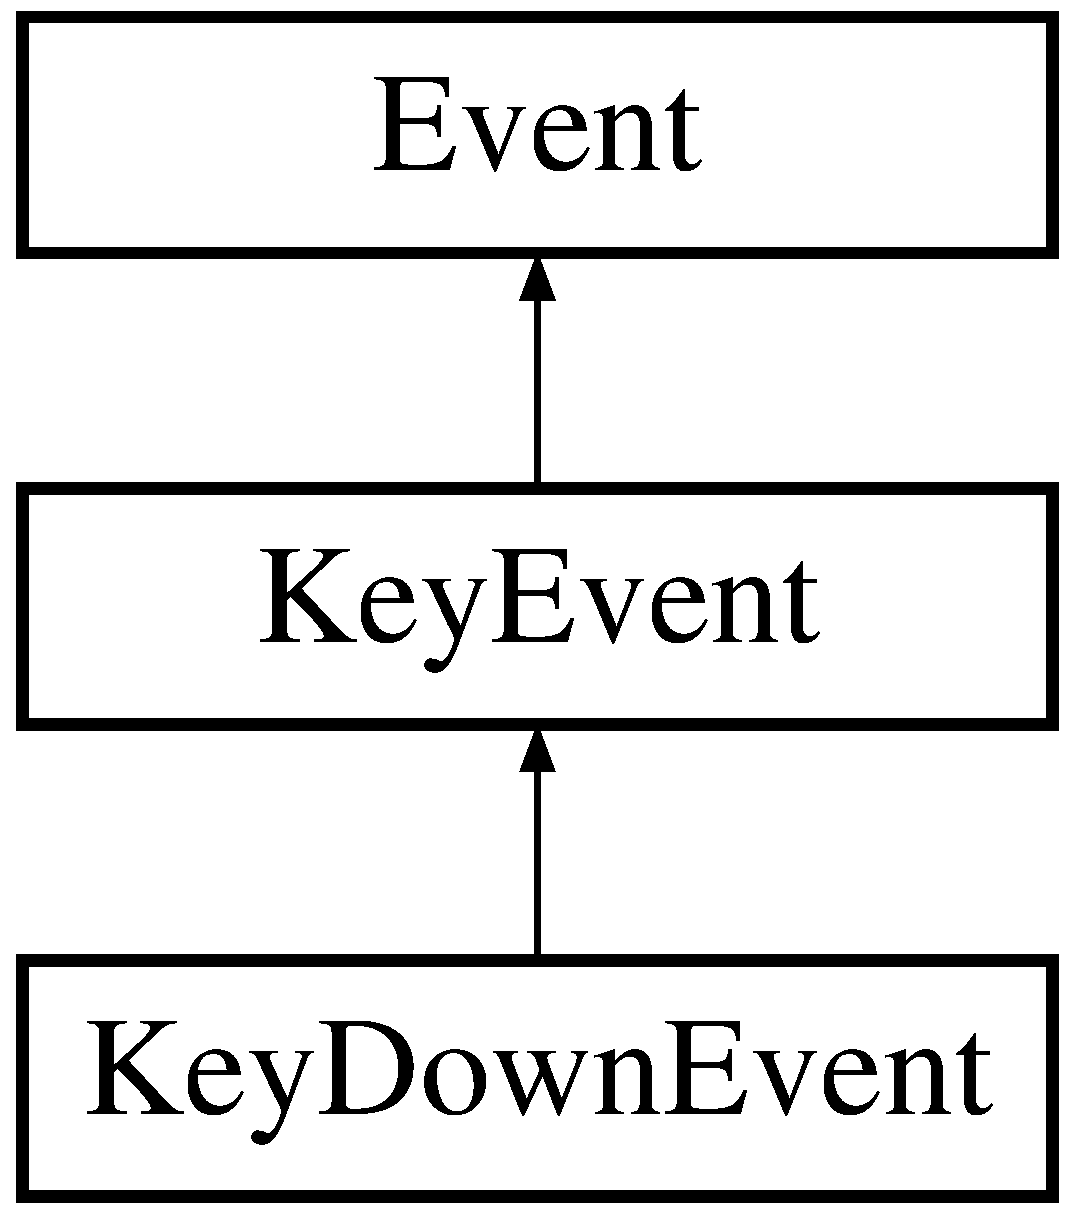
\includegraphics[height=3.000000cm]{classKeyDownEvent}
\end{center}
\end{figure}
\subsection*{Public Member Functions}
\begin{DoxyCompactItemize}
\item 
\hyperlink{classKeyDownEvent_ae27c2dfd549d9ea2ffd270e566aece6a}{Key\+Down\+Event} (Keyboard\+Key key, Keyboard\+Modifiers mods, bool is\+Repetition=false)
\begin{DoxyCompactList}\small\item\em Write what the function does here. \end{DoxyCompactList}\item 
virtual bool \hyperlink{classKeyDownEvent_a0661aa3784232a84df40fd570b865a51}{dispatch} (shared\+\_\+ptr$<$ \hyperlink{structEventHandler}{Event\+Handler} $>$ event\+Handler) override
\begin{DoxyCompactList}\small\item\em Write what the function does here. \end{DoxyCompactList}\end{DoxyCompactItemize}
\subsection*{Public Attributes}
\begin{DoxyCompactItemize}
\item 
\hypertarget{classKeyDownEvent_aa9ad513136e6d324870e601bbea2f869}{const bool {\bfseries is\+Repetition}}\label{classKeyDownEvent_aa9ad513136e6d324870e601bbea2f869}

\end{DoxyCompactItemize}
\subsection*{Additional Inherited Members}


\subsection{Detailed Description}
Write what the function does here. 


\begin{DoxyRetVals}{Return values}
{\em (variable)} & (description of variable) \\
\hline
\end{DoxyRetVals}


Definition at line 118 of file event.\+h.



\subsection{Constructor \& Destructor Documentation}
\hypertarget{classKeyDownEvent_ae27c2dfd549d9ea2ffd270e566aece6a}{\index{Key\+Down\+Event@{Key\+Down\+Event}!Key\+Down\+Event@{Key\+Down\+Event}}
\index{Key\+Down\+Event@{Key\+Down\+Event}!Key\+Down\+Event@{Key\+Down\+Event}}
\subsubsection[{Key\+Down\+Event}]{\setlength{\rightskip}{0pt plus 5cm}Key\+Down\+Event\+::\+Key\+Down\+Event (
\begin{DoxyParamCaption}
\item[{Keyboard\+Key}]{key, }
\item[{Keyboard\+Modifiers}]{mods, }
\item[{bool}]{is\+Repetition = {\ttfamily false}}
\end{DoxyParamCaption}
)\hspace{0.3cm}{\ttfamily [inline]}}}\label{classKeyDownEvent_ae27c2dfd549d9ea2ffd270e566aece6a}


Write what the function does here. 


\begin{DoxyParams}{Parameters}
{\em key} & \\
\hline
{\em mods} & \\
\hline
{\em false} & \\
\hline
{\em Type\+\_\+\+Key\+Down} & \\
\hline
{\em key} & \\
\hline
{\em mods} & \\
\hline
{\em is\+Repetition} & \\
\hline
\end{DoxyParams}

\begin{DoxyRetVals}{Return values}
{\em (variable)} & (description of variable) \\
\hline
\end{DoxyRetVals}


Definition at line 136 of file event.\+h.


\begin{DoxyCode}
136                                                                                          : 
      \hyperlink{classKeyEvent_aea3a7d348f12de966dc7199d26a978b0}{KeyEvent}(Type\_KeyDown, key, mods), isRepetition(isRepetition)
137     \{
138     \}
\end{DoxyCode}


\subsection{Member Function Documentation}
\hypertarget{classKeyDownEvent_a0661aa3784232a84df40fd570b865a51}{\index{Key\+Down\+Event@{Key\+Down\+Event}!dispatch@{dispatch}}
\index{dispatch@{dispatch}!Key\+Down\+Event@{Key\+Down\+Event}}
\subsubsection[{dispatch}]{\setlength{\rightskip}{0pt plus 5cm}virtual bool Key\+Down\+Event\+::dispatch (
\begin{DoxyParamCaption}
\item[{shared\+\_\+ptr$<$ {\bf Event\+Handler} $>$}]{event\+Handler}
\end{DoxyParamCaption}
)\hspace{0.3cm}{\ttfamily [inline]}, {\ttfamily [override]}, {\ttfamily [virtual]}}}\label{classKeyDownEvent_a0661aa3784232a84df40fd570b865a51}


Write what the function does here. 


\begin{DoxyParams}{Parameters}
{\em event\+Handler} & \\
\hline
\end{DoxyParams}

\begin{DoxyRetVals}{Return values}
{\em (variable)} & (description of variable) \\
\hline
\end{DoxyRetVals}


Implements \hyperlink{classEvent}{Event}.



Definition at line 147 of file event.\+h.


\begin{DoxyCode}
148         \{
149             \textcolor{keywordflow}{return} eventHandler->handleKeyDown(*\textcolor{keyword}{this});
150         \}
\end{DoxyCode}


The documentation for this class was generated from the following file\+:\begin{DoxyCompactItemize}
\item 
event.\+h\end{DoxyCompactItemize}

\hypertarget{classKeyEvent}{\section{Key\+Event Class Reference}
\label{classKeyEvent}\index{Key\+Event@{Key\+Event}}
}


Write what the function does here.  




{\ttfamily \#include $<$event.\+h$>$}

Inheritance diagram for Key\+Event\+:\begin{figure}[H]
\begin{center}
\leavevmode
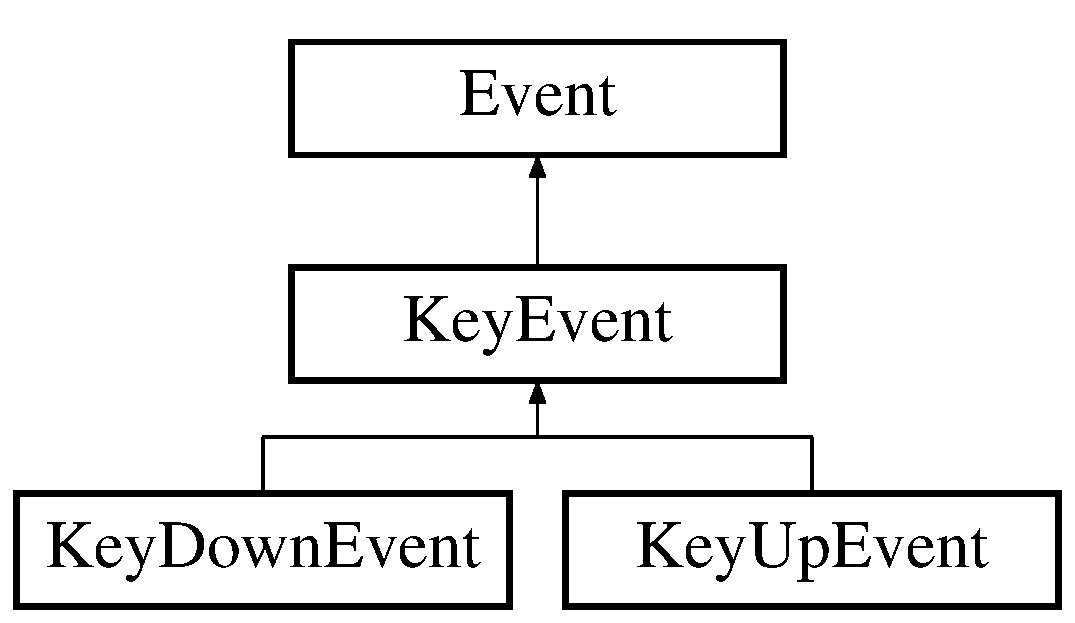
\includegraphics[height=3.000000cm]{classKeyEvent}
\end{center}
\end{figure}
\subsection*{Public Attributes}
\begin{DoxyCompactItemize}
\item 
\hypertarget{classKeyEvent_a99640b48450650dae71b55031b6382d0}{const Keyboard\+Key {\bfseries key}}\label{classKeyEvent_a99640b48450650dae71b55031b6382d0}

\item 
\hypertarget{classKeyEvent_ae5f742fee74ca2ed833fee6f301ba707}{const Keyboard\+Modifiers {\bfseries mods}}\label{classKeyEvent_ae5f742fee74ca2ed833fee6f301ba707}

\end{DoxyCompactItemize}
\subsection*{Protected Member Functions}
\begin{DoxyCompactItemize}
\item 
\hyperlink{classKeyEvent_aea3a7d348f12de966dc7199d26a978b0}{Key\+Event} (\hyperlink{classEvent_a2abf13b5be49315e9e362af02029f058}{Type} type, Keyboard\+Key key, Keyboard\+Modifiers mods)
\begin{DoxyCompactList}\small\item\em Write what the function does here. \end{DoxyCompactList}\end{DoxyCompactItemize}
\subsection*{Additional Inherited Members}


\subsection{Detailed Description}
Write what the function does here. 


\begin{DoxyRetVals}{Return values}
{\em (variable)} & (description of variable) \\
\hline
\end{DoxyRetVals}


Definition at line 89 of file event.\+h.



\subsection{Constructor \& Destructor Documentation}
\hypertarget{classKeyEvent_aea3a7d348f12de966dc7199d26a978b0}{\index{Key\+Event@{Key\+Event}!Key\+Event@{Key\+Event}}
\index{Key\+Event@{Key\+Event}!Key\+Event@{Key\+Event}}
\subsubsection[{Key\+Event}]{\setlength{\rightskip}{0pt plus 5cm}Key\+Event\+::\+Key\+Event (
\begin{DoxyParamCaption}
\item[{{\bf Type}}]{type, }
\item[{Keyboard\+Key}]{key, }
\item[{Keyboard\+Modifiers}]{mods}
\end{DoxyParamCaption}
)\hspace{0.3cm}{\ttfamily [inline]}, {\ttfamily [protected]}}}\label{classKeyEvent_aea3a7d348f12de966dc7199d26a978b0}


Write what the function does here. 


\begin{DoxyParams}{Parameters}
{\em type} & \\
\hline
{\em key} & \\
\hline
{\em mods} & \\
\hline
{\em type} & \\
\hline
{\em key} & \\
\hline
{\em mods} & \\
\hline
\end{DoxyParams}

\begin{DoxyRetVals}{Return values}
{\em (variable)} & (description of variable) \\
\hline
\end{DoxyRetVals}


Definition at line 108 of file event.\+h.


\begin{DoxyCode}
108                                                                     : \hyperlink{classEvent}{Event}(type), key(key), mods(mods
      )
109     \{
110     \}
\end{DoxyCode}


The documentation for this class was generated from the following file\+:\begin{DoxyCompactItemize}
\item 
event.\+h\end{DoxyCompactItemize}

\hypertarget{structKeyPressEvent}{\section{Key\+Press\+Event Struct Reference}
\label{structKeyPressEvent}\index{Key\+Press\+Event@{Key\+Press\+Event}}
}


Write what the function does here.  




{\ttfamily \#include $<$event.\+h$>$}

Inheritance diagram for Key\+Press\+Event\+:\begin{figure}[H]
\begin{center}
\leavevmode
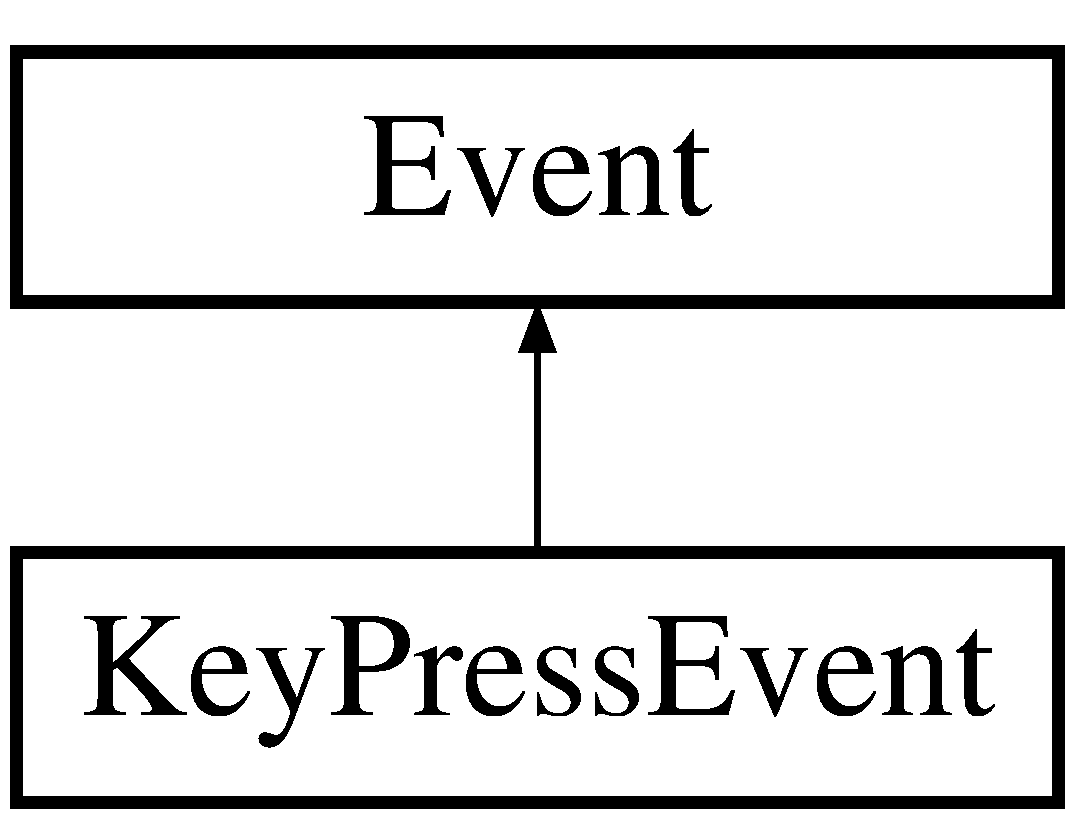
\includegraphics[height=2.000000cm]{structKeyPressEvent}
\end{center}
\end{figure}
\subsection*{Public Member Functions}
\begin{DoxyCompactItemize}
\item 
\hypertarget{structKeyPressEvent_a4d9766496d06b53ba5b594ed922082a8}{{\bfseries Key\+Press\+Event} (wchar\+\_\+t character)}\label{structKeyPressEvent_a4d9766496d06b53ba5b594ed922082a8}

\item 
virtual bool \hyperlink{structKeyPressEvent_a1c0e591880a4e20864a5d910e062c7fb}{dispatch} (shared\+\_\+ptr$<$ \hyperlink{structEventHandler}{Event\+Handler} $>$ event\+Handler) override
\begin{DoxyCompactList}\small\item\em Write what the function does here. \end{DoxyCompactList}\end{DoxyCompactItemize}
\subsection*{Public Attributes}
\begin{DoxyCompactItemize}
\item 
\hypertarget{structKeyPressEvent_a07fd7ffa0d7ab155ecaaed3cfb087b43}{const wchar\+\_\+t {\bfseries character}}\label{structKeyPressEvent_a07fd7ffa0d7ab155ecaaed3cfb087b43}

\end{DoxyCompactItemize}
\subsection*{Additional Inherited Members}


\subsection{Detailed Description}
Write what the function does here. 


\begin{DoxyRetVals}{Return values}
{\em (variable)} & (description of variable) \\
\hline
\end{DoxyRetVals}


Definition at line 184 of file event.\+h.



\subsection{Member Function Documentation}
\hypertarget{structKeyPressEvent_a1c0e591880a4e20864a5d910e062c7fb}{\index{Key\+Press\+Event@{Key\+Press\+Event}!dispatch@{dispatch}}
\index{dispatch@{dispatch}!Key\+Press\+Event@{Key\+Press\+Event}}
\subsubsection[{dispatch}]{\setlength{\rightskip}{0pt plus 5cm}virtual bool Key\+Press\+Event\+::dispatch (
\begin{DoxyParamCaption}
\item[{shared\+\_\+ptr$<$ {\bf Event\+Handler} $>$}]{event\+Handler}
\end{DoxyParamCaption}
)\hspace{0.3cm}{\ttfamily [inline]}, {\ttfamily [override]}, {\ttfamily [virtual]}}}\label{structKeyPressEvent_a1c0e591880a4e20864a5d910e062c7fb}


Write what the function does here. 


\begin{DoxyParams}{Parameters}
{\em event\+Handler} & \\
\hline
\end{DoxyParams}

\begin{DoxyRetVals}{Return values}
{\em (variable)} & (description of variable) \\
\hline
\end{DoxyRetVals}


Implements \hyperlink{classEvent}{Event}.



Definition at line 199 of file event.\+h.


\begin{DoxyCode}
200     \{
201         \textcolor{keywordflow}{return} eventHandler->handleKeyPress(*\textcolor{keyword}{this});
202     \}
\end{DoxyCode}


The documentation for this struct was generated from the following file\+:\begin{DoxyCompactItemize}
\item 
event.\+h\end{DoxyCompactItemize}

\hypertarget{classKeyUpEvent}{\section{Key\+Up\+Event Class Reference}
\label{classKeyUpEvent}\index{Key\+Up\+Event@{Key\+Up\+Event}}
}


Write what the function does here.  




{\ttfamily \#include $<$event.\+h$>$}

Inheritance diagram for Key\+Up\+Event\+:\begin{figure}[H]
\begin{center}
\leavevmode
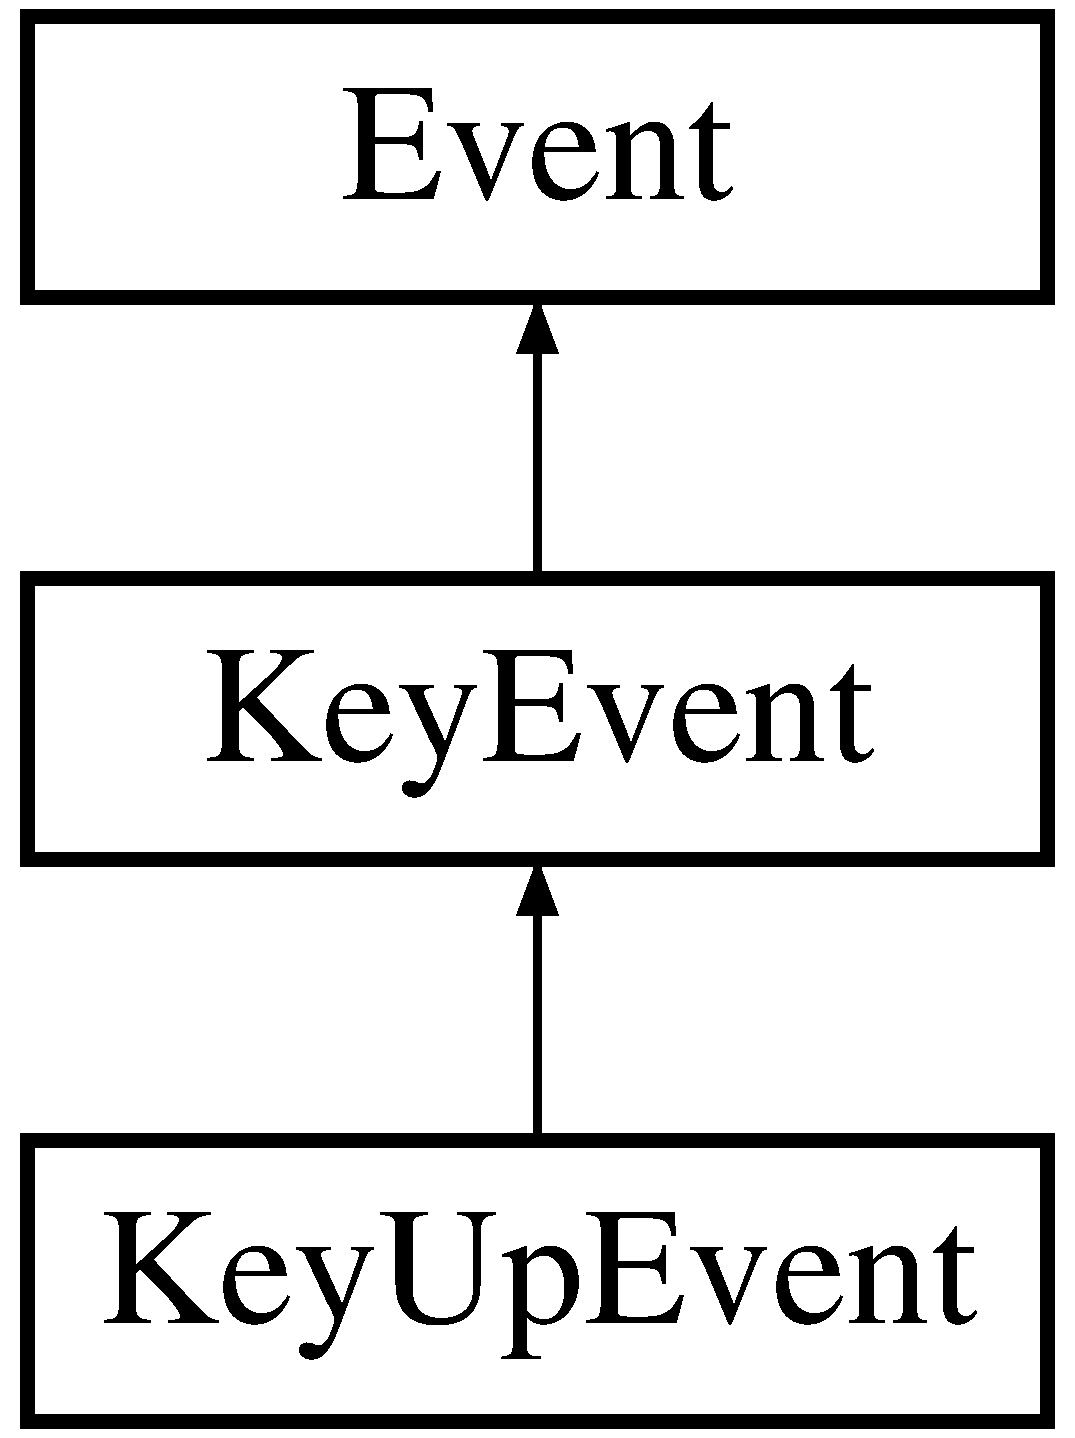
\includegraphics[height=3.000000cm]{classKeyUpEvent}
\end{center}
\end{figure}
\subsection*{Public Member Functions}
\begin{DoxyCompactItemize}
\item 
\hypertarget{classKeyUpEvent_a26f3177d7dc9887e87fbea4f5dded283}{{\bfseries Key\+Up\+Event} (Keyboard\+Key key, Keyboard\+Modifiers mods)}\label{classKeyUpEvent_a26f3177d7dc9887e87fbea4f5dded283}

\item 
virtual bool \hyperlink{classKeyUpEvent_a24d061fc9e6559908c91972376d4a3d4}{dispatch} (shared\+\_\+ptr$<$ \hyperlink{structEventHandler}{Event\+Handler} $>$ event\+Handler) override
\begin{DoxyCompactList}\small\item\em Write what the function does here. \end{DoxyCompactList}\end{DoxyCompactItemize}
\subsection*{Additional Inherited Members}


\subsection{Detailed Description}
Write what the function does here. 


\begin{DoxyRetVals}{Return values}
{\em (variable)} & (description of variable) \\
\hline
\end{DoxyRetVals}


Definition at line 158 of file event.\+h.



\subsection{Member Function Documentation}
\hypertarget{classKeyUpEvent_a24d061fc9e6559908c91972376d4a3d4}{\index{Key\+Up\+Event@{Key\+Up\+Event}!dispatch@{dispatch}}
\index{dispatch@{dispatch}!Key\+Up\+Event@{Key\+Up\+Event}}
\subsubsection[{dispatch}]{\setlength{\rightskip}{0pt plus 5cm}virtual bool Key\+Up\+Event\+::dispatch (
\begin{DoxyParamCaption}
\item[{shared\+\_\+ptr$<$ {\bf Event\+Handler} $>$}]{event\+Handler}
\end{DoxyParamCaption}
)\hspace{0.3cm}{\ttfamily [inline]}, {\ttfamily [override]}, {\ttfamily [virtual]}}}\label{classKeyUpEvent_a24d061fc9e6559908c91972376d4a3d4}


Write what the function does here. 


\begin{DoxyParams}{Parameters}
{\em event\+Handler} & \\
\hline
\end{DoxyParams}

\begin{DoxyRetVals}{Return values}
{\em (variable)} & (description of variable) \\
\hline
\end{DoxyRetVals}


Implements \hyperlink{classEvent}{Event}.



Definition at line 173 of file event.\+h.


\begin{DoxyCode}
174         \{
175             \textcolor{keywordflow}{return} eventHandler->handleKeyUp(*\textcolor{keyword}{this});
176         \}
\end{DoxyCode}


The documentation for this class was generated from the following file\+:\begin{DoxyCompactItemize}
\item 
event.\+h\end{DoxyCompactItemize}

\hypertarget{structKnob}{\section{Knob Struct Reference}
\label{structKnob}\index{Knob@{Knob}}
}
\subsection*{Public Attributes}
\begin{DoxyCompactItemize}
\item 
\hypertarget{structKnob_a030d68426750322c24409d4c88504d25}{float {\bfseries ang}}\label{structKnob_a030d68426750322c24409d4c88504d25}

\item 
\hypertarget{structKnob_a380ea778571da22f6e94f870a3f74a02}{float {\bfseries r}}\label{structKnob_a380ea778571da22f6e94f870a3f74a02}

\item 
\hypertarget{structKnob_ac445bc23490fc67bbb13725af6e3d9c3}{\hyperlink{structPoint}{Point} {\bfseries p}}\label{structKnob_ac445bc23490fc67bbb13725af6e3d9c3}

\end{DoxyCompactItemize}


\subsection{Detailed Description}


Definition at line 69 of file testgesture.\+c.



The documentation for this struct was generated from the following file\+:\begin{DoxyCompactItemize}
\item 
S\+D\+L2-\/2.\+0.\+3/test/testgesture.\+c\end{DoxyCompactItemize}

\hypertarget{classLineFind}{\section{Line\+Find Class Reference}
\label{classLineFind}\index{Line\+Find@{Line\+Find}}
}
\subsection*{Public Member Functions}
\begin{DoxyCompactItemize}
\item 
\hypertarget{classLineFind_a3d82021934c4f169775ff547abb26f3d}{{\bfseries Line\+Find} (const Line $\ast$line)}\label{classLineFind_a3d82021934c4f169775ff547abb26f3d}

\item 
\hypertarget{classLineFind_a5c26eeb76e5e61254ea40ccc7e548ae1}{bool {\bfseries operator()} (\hyperlink{structConnection}{Connection} $\ast$search)}\label{classLineFind_a5c26eeb76e5e61254ea40ccc7e548ae1}

\end{DoxyCompactItemize}
\subsection*{Private Attributes}
\begin{DoxyCompactItemize}
\item 
\hypertarget{classLineFind_a6d7da994468b7665a43bd43f9e6c8c1f}{const Line $\ast$ {\bfseries line}}\label{classLineFind_a6d7da994468b7665a43bd43f9e6c8c1f}

\end{DoxyCompactItemize}


\subsection{Detailed Description}


Definition at line 17 of file node.\+h.



The documentation for this class was generated from the following file\+:\begin{DoxyCompactItemize}
\item 
headers/node.\+h\end{DoxyCompactItemize}

\hypertarget{structLoadedPicture}{\section{Loaded\+Picture Struct Reference}
\label{structLoadedPicture}\index{Loaded\+Picture@{Loaded\+Picture}}
}
\subsection*{Public Attributes}
\begin{DoxyCompactItemize}
\item 
\hypertarget{structLoadedPicture_ad188d869ded0ab54d5f4e749fd3f885a}{\hyperlink{structSDL__Surface}{S\+D\+L\+\_\+\+Surface} $\ast$ {\bfseries surface}}\label{structLoadedPicture_ad188d869ded0ab54d5f4e749fd3f885a}

\item 
\hypertarget{structLoadedPicture_a88f8510bffd2294afa86748e316f1812}{S\+D\+L\+\_\+\+Texture $\ast$ {\bfseries texture}}\label{structLoadedPicture_a88f8510bffd2294afa86748e316f1812}

\item 
\hypertarget{structLoadedPicture_ac610a9b081d66683923d42d2edd4875f}{\hyperlink{structSDL__WindowShapeMode}{S\+D\+L\+\_\+\+Window\+Shape\+Mode} {\bfseries mode}}\label{structLoadedPicture_ac610a9b081d66683923d42d2edd4875f}

\item 
\hypertarget{structLoadedPicture_ad0dee7676eac82551b3083a47cf8de14}{const char $\ast$ {\bfseries name}}\label{structLoadedPicture_ad0dee7676eac82551b3083a47cf8de14}

\end{DoxyCompactItemize}


\subsection{Detailed Description}


Definition at line 22 of file testshape.\+c.



The documentation for this struct was generated from the following file\+:\begin{DoxyCompactItemize}
\item 
S\+D\+L2-\/2.\+0.\+3/test/testshape.\+c\end{DoxyCompactItemize}

\hypertarget{structLZ77CodeType}{\section{L\+Z77\+Code\+Type Struct Reference}
\label{structLZ77CodeType}\index{L\+Z77\+Code\+Type@{L\+Z77\+Code\+Type}}
}


Write what the function does here.  




{\ttfamily \#include $<$compressed\+\_\+stream.\+h$>$}

\subsection*{Public Member Functions}
\begin{DoxyCompactItemize}
\item 
\hypertarget{structLZ77CodeType_a3f8c29e5f88aff1053705e5a651a443f}{{\bfseries L\+Z77\+Code\+Type} (size\+\_\+t length, size\+\_\+t offset, uint8\+\_\+t next\+Byte)}\label{structLZ77CodeType_a3f8c29e5f88aff1053705e5a651a443f}

\item 
\hypertarget{structLZ77CodeType_a008eb3e8953c86bf3ae044c6824321cc}{{\bfseries L\+Z77\+Code\+Type} (uint8\+\_\+t next\+Byte)}\label{structLZ77CodeType_a008eb3e8953c86bf3ae044c6824321cc}

\item 
bool \hyperlink{structLZ77CodeType_a36290b0883b9280e74fab0f2a051bdd6}{has\+Next\+Byte} ()
\begin{DoxyCompactList}\small\item\em Write what the function does here. \end{DoxyCompactList}\item 
bool \hyperlink{structLZ77CodeType_a7277c9ee60156ee1b577d9b30cac3402}{eof} ()
\begin{DoxyCompactList}\small\item\em Write what the function does here. \end{DoxyCompactList}\item 
void \hyperlink{structLZ77CodeType_adf2ddd7196f0b8a4e60cddfccb60795c}{write} (\hyperlink{classWriter}{Writer} \&writer)
\begin{DoxyCompactList}\small\item\em Write what the function does here. \end{DoxyCompactList}\end{DoxyCompactItemize}
\subsection*{Static Public Member Functions}
\begin{DoxyCompactItemize}
\item 
static \hyperlink{structLZ77CodeType}{L\+Z77\+Code\+Type} \hyperlink{structLZ77CodeType_a81a3dc5f81b7ab0f7fc8ddfe80dca56f}{read} (\hyperlink{classReader}{Reader} \&reader)
\begin{DoxyCompactList}\small\item\em Write what the function does here. \end{DoxyCompactList}\end{DoxyCompactItemize}
\subsection*{Public Attributes}
\begin{DoxyCompactItemize}
\item 
\hypertarget{structLZ77CodeType_a1293f16ab8da36535682268031ec12a2}{size\+\_\+t {\bfseries length}}\label{structLZ77CodeType_a1293f16ab8da36535682268031ec12a2}

\item 
\hypertarget{structLZ77CodeType_a99e75c41fc2a5d36496e2eb6c675e8ce}{size\+\_\+t {\bfseries offset}}\label{structLZ77CodeType_a99e75c41fc2a5d36496e2eb6c675e8ce}

\item 
\hypertarget{structLZ77CodeType_ad5e0d80546417194466ff5300d0abc6f}{uint8\+\_\+t {\bfseries next\+Byte}}\label{structLZ77CodeType_ad5e0d80546417194466ff5300d0abc6f}

\end{DoxyCompactItemize}
\subsection*{Static Public Attributes}
\begin{DoxyCompactItemize}
\item 
\hypertarget{structLZ77CodeType_af6ddc790f261e742edf7e4c9730f2428}{static constexpr int {\bfseries length\+Bits} = 6}\label{structLZ77CodeType_af6ddc790f261e742edf7e4c9730f2428}

\item 
\hypertarget{structLZ77CodeType_a73491cf97e707f632e18d331d88c9aec}{static constexpr int {\bfseries offset\+Bits} = 16 -\/ length\+Bits}\label{structLZ77CodeType_a73491cf97e707f632e18d331d88c9aec}

\item 
\hypertarget{structLZ77CodeType_a91907290a8a919c21b5312ece5fe5eb4}{static constexpr size\+\_\+t {\bfseries max\+Length} = (1 $<$$<$ length\+Bits) -\/ 1}\label{structLZ77CodeType_a91907290a8a919c21b5312ece5fe5eb4}

\item 
\hypertarget{structLZ77CodeType_a07cb40a10cc2f689a9323c0f6533ed3c}{static constexpr size\+\_\+t {\bfseries max\+Offset} = (1 $<$$<$ offset\+Bits) -\/ 1}\label{structLZ77CodeType_a07cb40a10cc2f689a9323c0f6533ed3c}

\end{DoxyCompactItemize}


\subsection{Detailed Description}
Write what the function does here. 

\begin{DoxyReturn}{Returns}

\end{DoxyReturn}


Definition at line 26 of file compressed\+\_\+stream.\+h.



\subsection{Member Function Documentation}
\hypertarget{structLZ77CodeType_a7277c9ee60156ee1b577d9b30cac3402}{\index{L\+Z77\+Code\+Type@{L\+Z77\+Code\+Type}!eof@{eof}}
\index{eof@{eof}!L\+Z77\+Code\+Type@{L\+Z77\+Code\+Type}}
\subsubsection[{eof}]{\setlength{\rightskip}{0pt plus 5cm}bool L\+Z77\+Code\+Type\+::eof (
\begin{DoxyParamCaption}
{}
\end{DoxyParamCaption}
)\hspace{0.3cm}{\ttfamily [inline]}}}\label{structLZ77CodeType_a7277c9ee60156ee1b577d9b30cac3402}


Write what the function does here. 

\begin{DoxyReturn}{Returns}

\end{DoxyReturn}


Definition at line 61 of file compressed\+\_\+stream.\+h.


\begin{DoxyCode}
62     \{
63         \textcolor{keywordflow}{return} length == 0 && offset != 0;
64     \}
\end{DoxyCode}
\hypertarget{structLZ77CodeType_a36290b0883b9280e74fab0f2a051bdd6}{\index{L\+Z77\+Code\+Type@{L\+Z77\+Code\+Type}!has\+Next\+Byte@{has\+Next\+Byte}}
\index{has\+Next\+Byte@{has\+Next\+Byte}!L\+Z77\+Code\+Type@{L\+Z77\+Code\+Type}}
\subsubsection[{has\+Next\+Byte}]{\setlength{\rightskip}{0pt plus 5cm}bool L\+Z77\+Code\+Type\+::has\+Next\+Byte (
\begin{DoxyParamCaption}
{}
\end{DoxyParamCaption}
)\hspace{0.3cm}{\ttfamily [inline]}}}\label{structLZ77CodeType_a36290b0883b9280e74fab0f2a051bdd6}


Write what the function does here. 

\begin{DoxyReturn}{Returns}

\end{DoxyReturn}


Definition at line 51 of file compressed\+\_\+stream.\+h.


\begin{DoxyCode}
52     \{
53         \textcolor{keywordflow}{return} length != 0 || offset == 0;
54     \}
\end{DoxyCode}
\hypertarget{structLZ77CodeType_a81a3dc5f81b7ab0f7fc8ddfe80dca56f}{\index{L\+Z77\+Code\+Type@{L\+Z77\+Code\+Type}!read@{read}}
\index{read@{read}!L\+Z77\+Code\+Type@{L\+Z77\+Code\+Type}}
\subsubsection[{read}]{\setlength{\rightskip}{0pt plus 5cm}static {\bf L\+Z77\+Code\+Type} L\+Z77\+Code\+Type\+::read (
\begin{DoxyParamCaption}
\item[{{\bf Reader} \&}]{reader}
\end{DoxyParamCaption}
)\hspace{0.3cm}{\ttfamily [inline]}, {\ttfamily [static]}}}\label{structLZ77CodeType_a81a3dc5f81b7ab0f7fc8ddfe80dca56f}


Write what the function does here. 


\begin{DoxyParams}{Parameters}
{\em reader} & \\
\hline
\end{DoxyParams}
\begin{DoxyReturn}{Returns}

\end{DoxyReturn}


Definition at line 73 of file compressed\+\_\+stream.\+h.



References Reader\+::read\+U16().


\begin{DoxyCode}
74     \{
75         \hyperlink{structLZ77CodeType}{LZ77CodeType} retval;
76         retval.nextByte = reader.readByte();
77 
78         \textcolor{keywordflow}{try}
79         \{
80             uint16\_t v = reader.\hyperlink{classReader_afd87a9f4420fdf4d6bd5d311c745df92}{readU16}();
81             retval.length = v >> offsetBits;
82             retval.offset = v & maxOffset;
83         \}
84 
85         \textcolor{keywordflow}{catch}(\hyperlink{classEOFException}{EOFException} &e)
86         \{
87             \textcolor{keywordflow}{throw} \hyperlink{classLZ77FormatException}{LZ77FormatException}();
88         \}
89         \textcolor{keywordflow}{return} retval;
90     \}
\end{DoxyCode}
\hypertarget{structLZ77CodeType_adf2ddd7196f0b8a4e60cddfccb60795c}{\index{L\+Z77\+Code\+Type@{L\+Z77\+Code\+Type}!write@{write}}
\index{write@{write}!L\+Z77\+Code\+Type@{L\+Z77\+Code\+Type}}
\subsubsection[{write}]{\setlength{\rightskip}{0pt plus 5cm}void L\+Z77\+Code\+Type\+::write (
\begin{DoxyParamCaption}
\item[{{\bf Writer} \&}]{writer}
\end{DoxyParamCaption}
)\hspace{0.3cm}{\ttfamily [inline]}}}\label{structLZ77CodeType_adf2ddd7196f0b8a4e60cddfccb60795c}


Write what the function does here. 


\begin{DoxyParams}{Parameters}
{\em writer} & \\
\hline
\end{DoxyParams}


Definition at line 97 of file compressed\+\_\+stream.\+h.



References Writer\+::write\+U16().


\begin{DoxyCode}
98     \{
99         \textcolor{comment}{//cout << "Write code : 0x" << hex << (unsigned)nextByte << dec << " : length : " << length << " :
       offset : " << offset << endl;}
100         writer.writeByte(nextByte);
101         uint16\_t v = (offset & maxOffset) | (length << offsetBits);
102         writer.\hyperlink{classWriter_a87898dff934c55c144149029173fe66f}{writeU16}(v);
103     \}
\end{DoxyCode}


The documentation for this struct was generated from the following file\+:\begin{DoxyCompactItemize}
\item 
compressed\+\_\+stream.\+h\end{DoxyCompactItemize}

\hypertarget{classLZ77FormatException}{\section{L\+Z77\+Format\+Exception Class Reference}
\label{classLZ77FormatException}\index{L\+Z77\+Format\+Exception@{L\+Z77\+Format\+Exception}}
}


Write what the function does here.  




{\ttfamily \#include $<$compressed\+\_\+stream.\+h$>$}

Inheritance diagram for L\+Z77\+Format\+Exception\+:\begin{figure}[H]
\begin{center}
\leavevmode
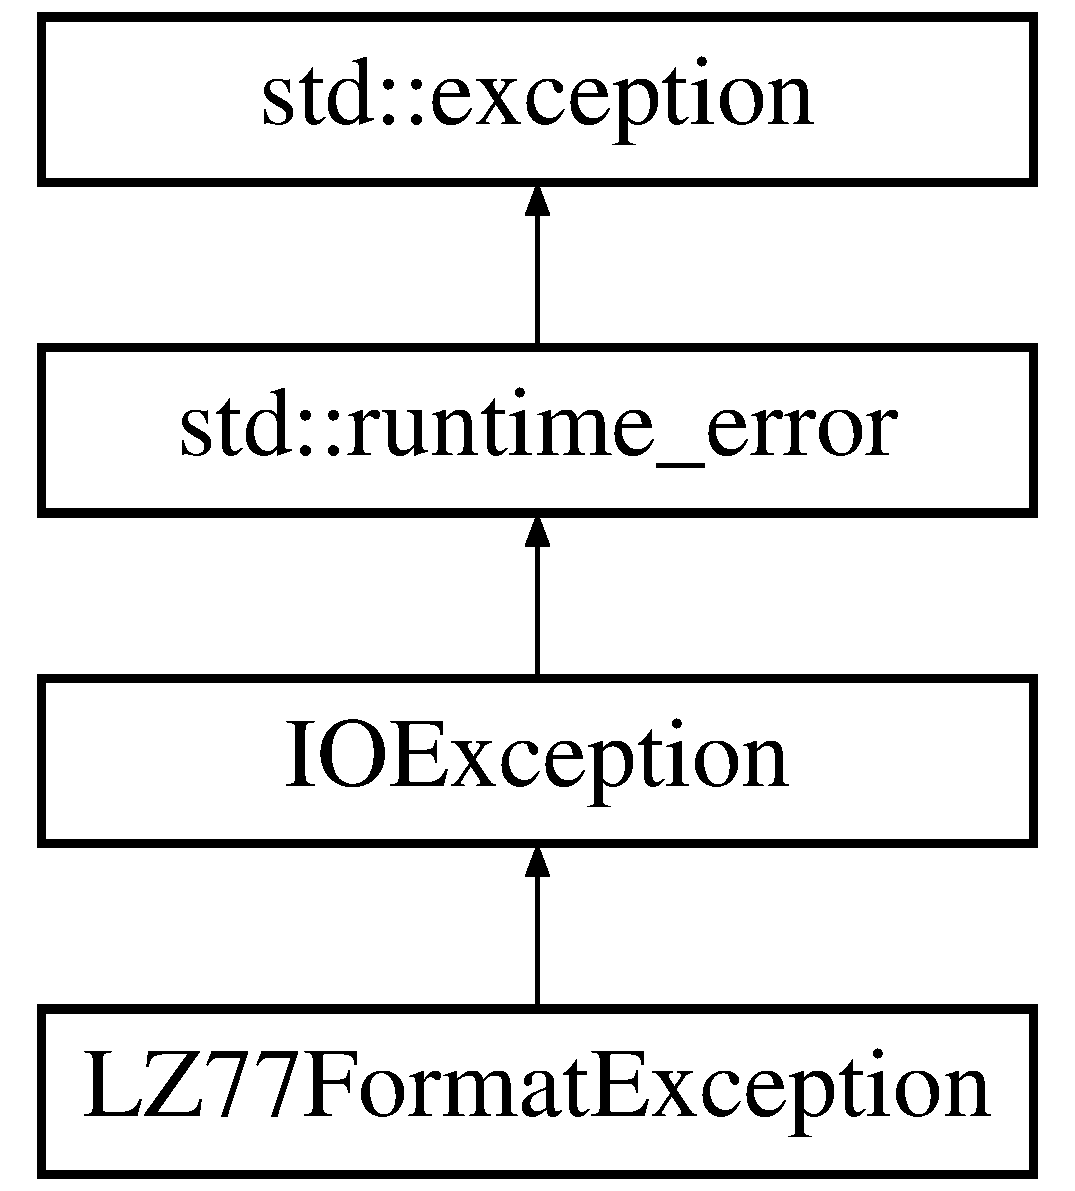
\includegraphics[height=4.000000cm]{classLZ77FormatException}
\end{center}
\end{figure}
\subsection*{Public Member Functions}
\begin{DoxyCompactItemize}
\item 
\hyperlink{classLZ77FormatException_ad7d83449811bccd5172e5ba76960d3d3}{L\+Z77\+Format\+Exception} ()
\begin{DoxyCompactList}\small\item\em Write what the function does here. \end{DoxyCompactList}\end{DoxyCompactItemize}


\subsection{Detailed Description}
Write what the function does here. 

\begin{DoxyReturn}{Returns}

\end{DoxyReturn}


Definition at line 12 of file compressed\+\_\+stream.\+h.



\subsection{Constructor \& Destructor Documentation}
\hypertarget{classLZ77FormatException_ad7d83449811bccd5172e5ba76960d3d3}{\index{L\+Z77\+Format\+Exception@{L\+Z77\+Format\+Exception}!L\+Z77\+Format\+Exception@{L\+Z77\+Format\+Exception}}
\index{L\+Z77\+Format\+Exception@{L\+Z77\+Format\+Exception}!L\+Z77\+Format\+Exception@{L\+Z77\+Format\+Exception}}
\subsubsection[{L\+Z77\+Format\+Exception}]{\setlength{\rightskip}{0pt plus 5cm}L\+Z77\+Format\+Exception\+::\+L\+Z77\+Format\+Exception (
\begin{DoxyParamCaption}
{}
\end{DoxyParamCaption}
)\hspace{0.3cm}{\ttfamily [inline]}}}\label{classLZ77FormatException_ad7d83449811bccd5172e5ba76960d3d3}


Write what the function does here. 

\begin{DoxyReturn}{Returns}

\end{DoxyReturn}


Definition at line 15 of file compressed\+\_\+stream.\+h.


\begin{DoxyCode}
22             : \hyperlink{classIOException_a73fcf78b1b5820aa158680e896f0b983}{IOException}(\textcolor{stringliteral}{"LZ77 format error"})
23             \{
24             \}
\end{DoxyCode}


The documentation for this class was generated from the following file\+:\begin{DoxyCompactItemize}
\item 
compressed\+\_\+stream.\+h\end{DoxyCompactItemize}

\hypertarget{structMappingStep}{\section{Mapping\+Step Struct Reference}
\label{structMappingStep}\index{Mapping\+Step@{Mapping\+Step}}
}
\subsection*{Public Attributes}
\begin{DoxyCompactItemize}
\item 
\hypertarget{structMappingStep_ac122b5c527e4ae777eff7b2bfdde2d49}{int {\bfseries x}}\label{structMappingStep_ac122b5c527e4ae777eff7b2bfdde2d49}

\item 
\hypertarget{structMappingStep_a3a86d7dfdeb19ef69f22ccdf370fec9c}{int {\bfseries y}}\label{structMappingStep_a3a86d7dfdeb19ef69f22ccdf370fec9c}

\item 
\hypertarget{structMappingStep_a574c6544b75cee4daa9b37e327882e9a}{double {\bfseries angle}}\label{structMappingStep_a574c6544b75cee4daa9b37e327882e9a}

\item 
\hypertarget{structMappingStep_ac8229aaee7afea8812b1f086d4102627}{int {\bfseries marker}}\label{structMappingStep_ac8229aaee7afea8812b1f086d4102627}

\item 
\hypertarget{structMappingStep_ad586ab3d773ca3670fb82197cd277357}{char $\ast$ {\bfseries field}}\label{structMappingStep_ad586ab3d773ca3670fb82197cd277357}

\item 
\hypertarget{structMappingStep_abde758906946d0b1fa4e6bbf24673c20}{int {\bfseries axis}}\label{structMappingStep_abde758906946d0b1fa4e6bbf24673c20}

\item 
\hypertarget{structMappingStep_a684bf4169e4d2a91c046470ac7a6f7b7}{int {\bfseries button}}\label{structMappingStep_a684bf4169e4d2a91c046470ac7a6f7b7}

\item 
\hypertarget{structMappingStep_a269b7267c576ad110fa8b6660e31f898}{int {\bfseries hat}}\label{structMappingStep_a269b7267c576ad110fa8b6660e31f898}

\item 
\hypertarget{structMappingStep_a2c608a8521ae6a4c38c241e4d3429221}{int {\bfseries hat\+\_\+value}}\label{structMappingStep_a2c608a8521ae6a4c38c241e4d3429221}

\item 
\hypertarget{structMappingStep_a33042563865c10ae64a1edaa18722ecb}{char {\bfseries mapping} \mbox{[}4096\mbox{]}}\label{structMappingStep_a33042563865c10ae64a1edaa18722ecb}

\end{DoxyCompactItemize}


\subsection{Detailed Description}


Definition at line 38 of file controllermap.\+c.



The documentation for this struct was generated from the following file\+:\begin{DoxyCompactItemize}
\item 
S\+D\+L2-\/2.\+0.\+3/test/controllermap.\+c\end{DoxyCompactItemize}

\hypertarget{structCompressWriter_1_1Match}{\section{Compress\+Writer\+:\+:Match Struct Reference}
\label{structCompressWriter_1_1Match}\index{Compress\+Writer\+::\+Match@{Compress\+Writer\+::\+Match}}
}
\subsection*{Public Member Functions}
\begin{DoxyCompactItemize}
\item 
\hypertarget{structCompressWriter_1_1Match_a3d6139303e8181564960d270c3b4ffd5}{{\bfseries Match} (size\+\_\+t location, size\+\_\+t length)}\label{structCompressWriter_1_1Match_a3d6139303e8181564960d270c3b4ffd5}

\end{DoxyCompactItemize}
\subsection*{Public Attributes}
\begin{DoxyCompactItemize}
\item 
\hypertarget{structCompressWriter_1_1Match_a902fb7b60d35bb8443540dda336add4a}{size\+\_\+t {\bfseries location}}\label{structCompressWriter_1_1Match_a902fb7b60d35bb8443540dda336add4a}

\item 
\hypertarget{structCompressWriter_1_1Match_aecb21869042cc75d89dfe4a58e7af34d}{size\+\_\+t {\bfseries length}}\label{structCompressWriter_1_1Match_aecb21869042cc75d89dfe4a58e7af34d}

\end{DoxyCompactItemize}


\subsection{Detailed Description}


Definition at line 175 of file compressed\+\_\+stream.\+h.



The documentation for this struct was generated from the following file\+:\begin{DoxyCompactItemize}
\item 
compressed\+\_\+stream.\+h\end{DoxyCompactItemize}

\hypertarget{classMatrix}{\section{Matrix Class Reference}
\label{classMatrix}\index{Matrix@{Matrix}}
}


Write what the function does here.  




{\ttfamily \#include $<$matrix.\+h$>$}

\subsection*{Public Member Functions}
\begin{DoxyCompactItemize}
\item 
float \hyperlink{classMatrix_a44c5cb86dbd3b1cceb4fb97f8a7162cf}{get} (const int x, const int y) const 
\begin{DoxyCompactList}\small\item\em Write what the function does here. \end{DoxyCompactList}\item 
void \hyperlink{classMatrix_afed63f439c03991f045224143dfea6bf}{set} (const int x, const int y, float value)
\begin{DoxyCompactList}\small\item\em Write what the function does here. \end{DoxyCompactList}\item 
\hyperlink{classMatrix_a795649d936f1eb2768d4a32f45c35c61}{Matrix} (float x00, float x10, float x20, float x30, float x01, float x11, float x21, float x31, float x02, float x12, float x22, float x32)
\item 
\hyperlink{classMatrix_a2dba13c45127354c9f75ef576f49269b}{Matrix} ()
\begin{DoxyCompactList}\small\item\em Write what the function does here. \end{DoxyCompactList}\item 
float \hyperlink{classMatrix_aadfa353962ca1bf43ed148d79cc71fc6}{determinant} () const 
\begin{DoxyCompactList}\small\item\em Write what the function does here. \end{DoxyCompactList}\item 
\hyperlink{classMatrix}{Matrix} \hyperlink{classMatrix_acaac7c3eb8f32224c07dcd620ca44e26}{invert} () const 
\begin{DoxyCompactList}\small\item\em Write what the function does here. \end{DoxyCompactList}\item 
\hyperlink{classMatrix}{Matrix} \hyperlink{classMatrix_ab915ae9d317df03b6731438f9add20d8}{concat} (\hyperlink{classMatrix}{Matrix} rt) const 
\begin{DoxyCompactList}\small\item\em Write what the function does here. \end{DoxyCompactList}\item 
\hyperlink{structVectorF}{Vector\+F} \hyperlink{classMatrix_ab7d05d1560328ca22ab4809299b6d128}{apply} (\hyperlink{structVectorF}{Vector\+F} v) const 
\begin{DoxyCompactList}\small\item\em Write what the function does here. \end{DoxyCompactList}\item 
\hyperlink{structVectorF}{Vector\+F} \hyperlink{classMatrix_a4c6d99e79768c1e3e01f1cf8ce143951}{apply\+To\+Normal} (\hyperlink{structVectorF}{Vector\+F} v) const 
\begin{DoxyCompactList}\small\item\em Write what the function does here. \end{DoxyCompactList}\end{DoxyCompactItemize}
\subsection*{Static Public Member Functions}
\begin{DoxyCompactItemize}
\item 
static \hyperlink{classMatrix}{Matrix} \hyperlink{classMatrix_ab84e2141cb9aeda01998b21b2c0d0319}{identity} ()
\begin{DoxyCompactList}\small\item\em Write what the function does here. \end{DoxyCompactList}\item 
static \hyperlink{classMatrix}{Matrix} \hyperlink{classMatrix_a5cd82d7b398de86eae8ba93c57630c8a}{rotate} (const \hyperlink{structVectorF}{Vector\+F} axis, const double angle)
\begin{DoxyCompactList}\small\item\em Write what the function does here. \end{DoxyCompactList}\item 
static \hyperlink{classMatrix}{Matrix} \hyperlink{classMatrix_abc63d4009ae96f03ad44545e9d1c3c81}{rotate\+X} (double angle)
\begin{DoxyCompactList}\small\item\em Write what the function does here. \end{DoxyCompactList}\item 
static \hyperlink{classMatrix}{Matrix} \hyperlink{classMatrix_a83ee280c509de4ff036d26e8ed11d52f}{rotate\+Y} (double angle)
\begin{DoxyCompactList}\small\item\em Write what the function does here. \end{DoxyCompactList}\item 
static \hyperlink{classMatrix}{Matrix} \hyperlink{classMatrix_a1b0199d040686543579e52695eb6da14}{rotate\+Z} (double angle)
\begin{DoxyCompactList}\small\item\em Write what the function does here. \end{DoxyCompactList}\item 
static \hyperlink{classMatrix}{Matrix} \hyperlink{classMatrix_adf246c47bce77c3c53b9e804ec475e35}{translate} (\hyperlink{structVectorF}{Vector\+F} position)
\begin{DoxyCompactList}\small\item\em Write what the function does here. \end{DoxyCompactList}\item 
static \hyperlink{classMatrix}{Matrix} \hyperlink{classMatrix_a77d32ea082434b9b04374af58f3d7007}{translate} (float x, float y, float z)
\begin{DoxyCompactList}\small\item\em Write what the function does here. \end{DoxyCompactList}\item 
static \hyperlink{classMatrix}{Matrix} \hyperlink{classMatrix_a1f36f7f62b8e99fea99880b6fc80a604}{scale} (float x, float y, float z)
\begin{DoxyCompactList}\small\item\em Write what the function does here. \end{DoxyCompactList}\item 
static \hyperlink{classMatrix}{Matrix} \hyperlink{classMatrix_a3420c2adfcea1a4ef5ae86d6875ef75e}{scale} (\hyperlink{structVectorF}{Vector\+F} s)
\begin{DoxyCompactList}\small\item\em Write what the function does here. \end{DoxyCompactList}\item 
static \hyperlink{classMatrix}{Matrix} \hyperlink{classMatrix_a1205b0fb62536a9b18a2c4ef6fc6a316}{scale} (float s)
\begin{DoxyCompactList}\small\item\em Write what the function does here. \end{DoxyCompactList}\item 
static \hyperlink{classMatrix}{Matrix} \hyperlink{classMatrix_a8198676e0d8fdc3d447f184260af7057}{theta\+Phi} (double theta, double phi)
\begin{DoxyCompactList}\small\item\em Write what the function does here. \end{DoxyCompactList}\end{DoxyCompactItemize}
\subsection*{Public Attributes}
\begin{DoxyCompactItemize}
\item 
\hypertarget{classMatrix_ae83b796149e7692ce40c1cbdf4dd6f09}{float {\bfseries x00}}\label{classMatrix_ae83b796149e7692ce40c1cbdf4dd6f09}

\item 
\hypertarget{classMatrix_a27444a60f9571b225f6b5ce12a5eca11}{float {\bfseries x10}}\label{classMatrix_a27444a60f9571b225f6b5ce12a5eca11}

\item 
\hypertarget{classMatrix_aeed1c8585b1117930be0ff04bb59b841}{float {\bfseries x20}}\label{classMatrix_aeed1c8585b1117930be0ff04bb59b841}

\item 
\hypertarget{classMatrix_aa7fd1be4eb967ca4a2dca1629913b320}{float {\bfseries x30}}\label{classMatrix_aa7fd1be4eb967ca4a2dca1629913b320}

\item 
\hypertarget{classMatrix_a0d61e61547844a875cbe7bbc9ac45655}{float {\bfseries x01}}\label{classMatrix_a0d61e61547844a875cbe7bbc9ac45655}

\item 
\hypertarget{classMatrix_a8ab47a8d3f04f391429640eee452f7a6}{float {\bfseries x11}}\label{classMatrix_a8ab47a8d3f04f391429640eee452f7a6}

\item 
\hypertarget{classMatrix_acee3423cbef48d33c2411d90c882a371}{float {\bfseries x21}}\label{classMatrix_acee3423cbef48d33c2411d90c882a371}

\item 
\hypertarget{classMatrix_a6f6dbdec61807b9ec97b5c43072d9a74}{float {\bfseries x31}}\label{classMatrix_a6f6dbdec61807b9ec97b5c43072d9a74}

\item 
\hypertarget{classMatrix_aececca699c796ad7b1dd2e52820218c3}{float {\bfseries x02}}\label{classMatrix_aececca699c796ad7b1dd2e52820218c3}

\item 
\hypertarget{classMatrix_a9d02b516fb5aace9e21be7ead5494b87}{float {\bfseries x12}}\label{classMatrix_a9d02b516fb5aace9e21be7ead5494b87}

\item 
\hypertarget{classMatrix_a86643f9e4ba0701c4c220ec6292fe426}{float {\bfseries x22}}\label{classMatrix_a86643f9e4ba0701c4c220ec6292fe426}

\item 
\hypertarget{classMatrix_a1b08b0cdc3390fcec6e9dc71d5156bac}{float {\bfseries x32}}\label{classMatrix_a1b08b0cdc3390fcec6e9dc71d5156bac}

\end{DoxyCompactItemize}
\subsection*{Friends}
\begin{DoxyCompactItemize}
\item 
\hyperlink{classMatrix}{Matrix} \hyperlink{classMatrix_aff21cecb1b3c4d8e3f3d525edebd7d5c}{inverse} (const \hyperlink{classMatrix}{Matrix} \&m)
\begin{DoxyCompactList}\small\item\em Write what the function does here. \end{DoxyCompactList}\end{DoxyCompactItemize}


\subsection{Detailed Description}
Write what the function does here. 

4x4 matrix for 3\+D transformation with last row always equal to \mbox{[}0 0 0 1\mbox{]}

\begin{DoxyAuthor}{Author}
jacob 
\end{DoxyAuthor}
\begin{DoxyReturn}{Returns}

\end{DoxyReturn}


Definition at line 14 of file matrix.\+h.



\subsection{Constructor \& Destructor Documentation}
\hypertarget{classMatrix_a795649d936f1eb2768d4a32f45c35c61}{\index{Matrix@{Matrix}!Matrix@{Matrix}}
\index{Matrix@{Matrix}!Matrix@{Matrix}}
\subsubsection[{Matrix}]{\setlength{\rightskip}{0pt plus 5cm}Matrix\+::\+Matrix (
\begin{DoxyParamCaption}
\item[{float}]{x00, }
\item[{float}]{x10, }
\item[{float}]{x20, }
\item[{float}]{x30, }
\item[{float}]{x01, }
\item[{float}]{x11, }
\item[{float}]{x21, }
\item[{float}]{x31, }
\item[{float}]{x02, }
\item[{float}]{x12, }
\item[{float}]{x22, }
\item[{float}]{x32}
\end{DoxyParamCaption}
)\hspace{0.3cm}{\ttfamily [inline]}}}\label{classMatrix_a795649d936f1eb2768d4a32f45c35c61}

\begin{DoxyParams}{Parameters}
{\em x32} & Write what the function does here\\
\hline
{\em x32} & \\
\hline
\end{DoxyParams}
\begin{DoxyReturn}{Returns}

\begin{DoxyItemize}
\item 
\end{DoxyItemize}
\end{DoxyReturn}


Definition at line 171 of file matrix.\+h.


\begin{DoxyCode}
191         \{
192             this->x00 = x00;
193             this->x10 = x10;
194             this->x20 = x20;
195             this->x30 = x30;
196             this->x01 = x01;
197             this->x11 = x11;
198             this->x21 = x21;
199             this->x31 = x31;
200             this->x02 = x02;
201             this->x12 = x12;
202             this->x22 = x22;
203             this->x32 = x32;
204         \}
\end{DoxyCode}
\hypertarget{classMatrix_a2dba13c45127354c9f75ef576f49269b}{\index{Matrix@{Matrix}!Matrix@{Matrix}}
\index{Matrix@{Matrix}!Matrix@{Matrix}}
\subsubsection[{Matrix}]{\setlength{\rightskip}{0pt plus 5cm}Matrix\+::\+Matrix (
\begin{DoxyParamCaption}
{}
\end{DoxyParamCaption}
)\hspace{0.3cm}{\ttfamily [inline]}}}\label{classMatrix_a2dba13c45127354c9f75ef576f49269b}


Write what the function does here. 

\begin{DoxyReturn}{Returns}

\end{DoxyReturn}


Definition at line 211 of file matrix.\+h.



Referenced by concat(), identity(), invert(), rotate(), scale(), and translate().


\begin{DoxyCode}
212         \{
213             this->x00 = 1;
214             this->x10 = 0;
215             this->x20 = 0;
216             this->x30 = 0;
217             this->x01 = 0;
218             this->x11 = 1;
219             this->x21 = 0;
220             this->x31 = 0;
221             this->x02 = 0;
222             this->x12 = 0;
223             this->x22 = 1;
224             this->x32 = 0;
225         \}
\end{DoxyCode}


\subsection{Member Function Documentation}
\hypertarget{classMatrix_ab7d05d1560328ca22ab4809299b6d128}{\index{Matrix@{Matrix}!apply@{apply}}
\index{apply@{apply}!Matrix@{Matrix}}
\subsubsection[{apply}]{\setlength{\rightskip}{0pt plus 5cm}{\bf Vector\+F} Matrix\+::apply (
\begin{DoxyParamCaption}
\item[{{\bf Vector\+F}}]{v}
\end{DoxyParamCaption}
) const\hspace{0.3cm}{\ttfamily [inline]}}}\label{classMatrix_ab7d05d1560328ca22ab4809299b6d128}


Write what the function does here. 


\begin{DoxyParams}{Parameters}
{\em v} & \\
\hline
\end{DoxyParams}
\begin{DoxyReturn}{Returns}

\end{DoxyReturn}


Definition at line 546 of file matrix.\+h.


\begin{DoxyCode}
547         \{
548             \textcolor{keywordflow}{return} \hyperlink{structVectorF}{VectorF}(v.x * this->x00 + v.y * this->x10 + v.z * this->x20
549                     + this->x30, v.x * this->x01 + v.y * this->x11 + v.z * this->x21
550                     + this->x31, v.x * this->x02 + v.y * this->x12 + v.z * this->x22
551                     + this->x32);
552         \}
\end{DoxyCode}
\hypertarget{classMatrix_a4c6d99e79768c1e3e01f1cf8ce143951}{\index{Matrix@{Matrix}!apply\+To\+Normal@{apply\+To\+Normal}}
\index{apply\+To\+Normal@{apply\+To\+Normal}!Matrix@{Matrix}}
\subsubsection[{apply\+To\+Normal}]{\setlength{\rightskip}{0pt plus 5cm}{\bf Vector\+F} Matrix\+::apply\+To\+Normal (
\begin{DoxyParamCaption}
\item[{{\bf Vector\+F}}]{v}
\end{DoxyParamCaption}
) const\hspace{0.3cm}{\ttfamily [inline]}}}\label{classMatrix_a4c6d99e79768c1e3e01f1cf8ce143951}


Write what the function does here. 


\begin{DoxyParams}{Parameters}
{\em v} & \\
\hline
\end{DoxyParams}
\begin{DoxyReturn}{Returns}

\end{DoxyReturn}


Definition at line 561 of file matrix.\+h.


\begin{DoxyCode}
562         \{
563             \textcolor{keywordflow}{return} normalize(\hyperlink{structVectorF}{VectorF}(v.x * this->x00 + v.y * this->x10 + v.z * this->x20, v.x
564                         * this->x01 + v.y * this->x11 + v.z * this->x21, v.x * this->x02
565                         + v.y * this->x12 + v.z * this->x22));
566         \}
\end{DoxyCode}
\hypertarget{classMatrix_ab915ae9d317df03b6731438f9add20d8}{\index{Matrix@{Matrix}!concat@{concat}}
\index{concat@{concat}!Matrix@{Matrix}}
\subsubsection[{concat}]{\setlength{\rightskip}{0pt plus 5cm}{\bf Matrix} Matrix\+::concat (
\begin{DoxyParamCaption}
\item[{{\bf Matrix}}]{rt}
\end{DoxyParamCaption}
) const\hspace{0.3cm}{\ttfamily [inline]}}}\label{classMatrix_ab915ae9d317df03b6731438f9add20d8}


Write what the function does here. 


\begin{DoxyParams}{Parameters}
{\em rt} & \\
\hline
\end{DoxyParams}
\begin{DoxyReturn}{Returns}

\end{DoxyReturn}


Definition at line 522 of file matrix.\+h.



References Matrix().



Referenced by theta\+Phi().


\begin{DoxyCode}
523         \{
524             \textcolor{keywordflow}{return} \hyperlink{classMatrix_a2dba13c45127354c9f75ef576f49269b}{Matrix}(this->x00 * rt.x00 + this->x01 * rt.x10 + this->x02
525                     * rt.x20, this->x10 * rt.x00 + this->x11 * rt.x10 + this->x12
526                     * rt.x20, this->x20 * rt.x00 + this->x21 * rt.x10 + this->x22
527                     * rt.x20, this->x30 * rt.x00 + this->x31 * rt.x10 + this->x32
528                     * rt.x20 + rt.x30, this->x00 * rt.x01 + this->x01 * rt.x11
529                     + this->x02 * rt.x21, this->x10 * rt.x01 + this->x11 * rt.x11
530                     + this->x12 * rt.x21, this->x20 * rt.x01 + this->x21 * rt.x11
531                     + this->x22 * rt.x21, this->x30 * rt.x01 + this->x31 * rt.x11
532                     + this->x32 * rt.x21 + rt.x31, this->x00 * rt.x02 + this->x01
533                     * rt.x12 + this->x02 * rt.x22, this->x10 * rt.x02 + this->x11
534                     * rt.x12 + this->x12 * rt.x22, this->x20 * rt.x02 + this->x21
535                     * rt.x12 + this->x22 * rt.x22, this->x30 * rt.x02 + this->x31
536                     * rt.x12 + this->x32 * rt.x22 + rt.x32);
537         \}
\end{DoxyCode}
\hypertarget{classMatrix_aadfa353962ca1bf43ed148d79cc71fc6}{\index{Matrix@{Matrix}!determinant@{determinant}}
\index{determinant@{determinant}!Matrix@{Matrix}}
\subsubsection[{determinant}]{\setlength{\rightskip}{0pt plus 5cm}float Matrix\+::determinant (
\begin{DoxyParamCaption}
{}
\end{DoxyParamCaption}
) const\hspace{0.3cm}{\ttfamily [inline]}}}\label{classMatrix_aadfa353962ca1bf43ed148d79cc71fc6}


Write what the function does here. 

\begin{DoxyReturn}{Returns}
the determinant of this matrix 


\end{DoxyReturn}


Definition at line 454 of file matrix.\+h.



Referenced by invert().


\begin{DoxyCode}
455         \{
456             \textcolor{keywordflow}{return} this->x00 * (this->x11 * this->x22 - this->x12 * this->x21)
457                 + this->x10 * (this->x02 * this->x21 - this->x01 * this->x22)
458                 + this->x20 * (this->x01 * this->x12 - this->x02 * this->x11);
459         \}
\end{DoxyCode}
\hypertarget{classMatrix_a44c5cb86dbd3b1cceb4fb97f8a7162cf}{\index{Matrix@{Matrix}!get@{get}}
\index{get@{get}!Matrix@{Matrix}}
\subsubsection[{get}]{\setlength{\rightskip}{0pt plus 5cm}float Matrix\+::get (
\begin{DoxyParamCaption}
\item[{const int}]{x, }
\item[{const int}]{y}
\end{DoxyParamCaption}
) const\hspace{0.3cm}{\ttfamily [inline]}}}\label{classMatrix_a44c5cb86dbd3b1cceb4fb97f8a7162cf}


Write what the function does here. 


\begin{DoxyParams}{Parameters}
{\em x} & \\
\hline
{\em y} & \\
\hline
\end{DoxyParams}
\begin{DoxyReturn}{Returns}

\end{DoxyReturn}


Definition at line 29 of file matrix.\+h.


\begin{DoxyCode}
30         \{
31 
32             \textcolor{keywordflow}{switch}(x)
33             \{
34                 \textcolor{keywordflow}{case} 0:
35 
36                     \textcolor{keywordflow}{switch}(y)
37                     \{
38                         \textcolor{keywordflow}{case} 0:
39                             \textcolor{keywordflow}{return} this->x00;
40                         \textcolor{keywordflow}{case} 1:
41                             \textcolor{keywordflow}{return} this->x01;
42                         \textcolor{keywordflow}{case} 2:
43                             \textcolor{keywordflow}{return} this->x02;
44                         \textcolor{keywordflow}{default}:
45                             \textcolor{keywordflow}{return} x == y ? 1 : 0;
46                     \}
47                 \textcolor{keywordflow}{case} 1:
48 
49                     \textcolor{keywordflow}{switch}(y)
50                     \{
51                         \textcolor{keywordflow}{case} 0:
52                             \textcolor{keywordflow}{return} this->x10;
53                         \textcolor{keywordflow}{case} 1:
54                             \textcolor{keywordflow}{return} this->x11;
55                         \textcolor{keywordflow}{case} 2:
56                             \textcolor{keywordflow}{return} this->x12;
57                         \textcolor{keywordflow}{default}:
58                             \textcolor{keywordflow}{return} x == y ? 1 : 0;
59                     \}
60                 \textcolor{keywordflow}{case} 2:
61 
62                     \textcolor{keywordflow}{switch}(y)
63                     \{
64                         \textcolor{keywordflow}{case} 0:
65                             \textcolor{keywordflow}{return} this->x20;
66                         \textcolor{keywordflow}{case} 1:
67                             \textcolor{keywordflow}{return} this->x21;
68                         \textcolor{keywordflow}{case} 2:
69                             \textcolor{keywordflow}{return} this->x22;
70                         \textcolor{keywordflow}{default}:
71                             \textcolor{keywordflow}{return} x == y ? 1 : 0;
72                     \}
73                 \textcolor{keywordflow}{case} 3:
74 
75                     \textcolor{keywordflow}{switch}(y)
76                     \{
77                         \textcolor{keywordflow}{case} 0:
78                             \textcolor{keywordflow}{return} this->x30;
79                         \textcolor{keywordflow}{case} 1:
80                             \textcolor{keywordflow}{return} this->x31;
81                         \textcolor{keywordflow}{case} 2:
82                             \textcolor{keywordflow}{return} this->x32;
83                         \textcolor{keywordflow}{default}:
84                             \textcolor{keywordflow}{return} x == y ? 1 : 0;
85                     \}
86                 \textcolor{keywordflow}{default}:
87                     \textcolor{keywordflow}{return} x == y ? 1 : 0;
88             \}
89         \}
\end{DoxyCode}
\hypertarget{classMatrix_ab84e2141cb9aeda01998b21b2c0d0319}{\index{Matrix@{Matrix}!identity@{identity}}
\index{identity@{identity}!Matrix@{Matrix}}
\subsubsection[{identity}]{\setlength{\rightskip}{0pt plus 5cm}static {\bf Matrix} Matrix\+::identity (
\begin{DoxyParamCaption}
{}
\end{DoxyParamCaption}
)\hspace{0.3cm}{\ttfamily [inline]}, {\ttfamily [static]}}}\label{classMatrix_ab84e2141cb9aeda01998b21b2c0d0319}


Write what the function does here. 

\begin{DoxyReturn}{Returns}

\end{DoxyReturn}


Definition at line 232 of file matrix.\+h.



References Matrix().


\begin{DoxyCode}
233         \{
234             \textcolor{keywordflow}{return} \hyperlink{classMatrix_a2dba13c45127354c9f75ef576f49269b}{Matrix}(1, 0, 0, 0, 0, 1, 0, 0, 0, 0, 1, 0);
235         \}
\end{DoxyCode}
\hypertarget{classMatrix_acaac7c3eb8f32224c07dcd620ca44e26}{\index{Matrix@{Matrix}!invert@{invert}}
\index{invert@{invert}!Matrix@{Matrix}}
\subsubsection[{invert}]{\setlength{\rightskip}{0pt plus 5cm}{\bf Matrix} Matrix\+::invert (
\begin{DoxyParamCaption}
{}
\end{DoxyParamCaption}
) const\hspace{0.3cm}{\ttfamily [inline]}}}\label{classMatrix_acaac7c3eb8f32224c07dcd620ca44e26}


Write what the function does here. 

\begin{DoxyReturn}{Returns}
the inverse of this matrix. 


\end{DoxyReturn}


Definition at line 467 of file matrix.\+h.



References determinant(), and Matrix().


\begin{DoxyCode}
468         \{
469             \textcolor{keywordtype}{float} det = \hyperlink{classMatrix_aadfa353962ca1bf43ed148d79cc71fc6}{determinant}();
470             \textcolor{keywordflow}{if}(det == 0.0f)
471                 \textcolor{keywordflow}{throw} domain\_error(\textcolor{stringliteral}{"can't invert singular matrix"});
472             \textcolor{keywordtype}{float} factor = 1.0f / det;
473             \textcolor{keywordflow}{return} \hyperlink{classMatrix_a2dba13c45127354c9f75ef576f49269b}{Matrix}((this->x11 * this->x22 - this->x12 * this->x21) * factor,
474                     (this->x12 * this->x20 - this->x10 * this->x22) * factor,
475                     (this->x10 * this->x21 - this->x11 * this->x20) * factor,
476                     (-this->x10 * this->x21 * this->x32 + this->x11
477                      * this->x20 * this->x32 + this->x10 * this->x22
478                      * this->x31 - this->x12 * this->x20 * this->x31
479                      - this->x11 * this->x22 * this->x30 + this->x12
480                      * this->x21 * this->x30)
481                     * factor,
482                     (this->x02 * this->x21 - this->x01 * this->x22) * factor,
483                     (this->x00 * this->x22 - this->x02 * this->x20) * factor,
484                     (this->x01 * this->x20 - this->x00 * this->x21) * factor,
485                     (this->x00 * this->x21 * this->x32 - this->x01 * this->x20
486                      * this->x32 - this->x00 * this->x22 * this->x31
487                      + this->x02 * this->x20 * this->x31 + this->x01
488                      * this->x22 * this->x30 - this->x02 * this->x21
489                      * this->x30)
490                     * factor,
491                     (this->x01 * this->x12 - this->x02 * this->x11) * factor,
492                     (this->x02 * this->x10 - this->x00 * this->x12) * factor,
493                     (this->x00 * this->x11 - this->x01 * this->x10) * factor,
494                     (-this->x00 * this->x11 * this->x32 + this->x01
495                      * this->x10 * this->x32 + this->x00 * this->x12
496                      * this->x31 - this->x02 * this->x10 * this->x31
497                      - this->x01 * this->x12 * this->x30 + this->x02
498                      * this->x11 * this->x30)
499                         * factor);
500         \}
\end{DoxyCode}
\hypertarget{classMatrix_a5cd82d7b398de86eae8ba93c57630c8a}{\index{Matrix@{Matrix}!rotate@{rotate}}
\index{rotate@{rotate}!Matrix@{Matrix}}
\subsubsection[{rotate}]{\setlength{\rightskip}{0pt plus 5cm}static {\bf Matrix} Matrix\+::rotate (
\begin{DoxyParamCaption}
\item[{const {\bf Vector\+F}}]{axis, }
\item[{const double}]{angle}
\end{DoxyParamCaption}
)\hspace{0.3cm}{\ttfamily [inline]}, {\ttfamily [static]}}}\label{classMatrix_a5cd82d7b398de86eae8ba93c57630c8a}


Write what the function does here. 

creates a rotation matrix


\begin{DoxyParams}{Parameters}
{\em axis} & axis to rotate around \\
\hline
{\em angle} & angle to rotate in radians \\
\hline
\end{DoxyParams}
\begin{DoxyReturn}{Returns}
the new rotation matrix 
\end{DoxyReturn}
\begin{DoxySeeAlso}{See also}
\hyperlink{classMatrix_abc63d4009ae96f03ad44545e9d1c3c81}{rotate\+X(double angle)} 

\hyperlink{classMatrix_a83ee280c509de4ff036d26e8ed11d52f}{rotate\+Y(double angle)} 

\hyperlink{classMatrix_a1b0199d040686543579e52695eb6da14}{rotate\+Z(double angle)} 
\end{DoxySeeAlso}

\begin{DoxyParams}{Parameters}
{\em axis} & \\
\hline
{\em angle} & \\
\hline
\end{DoxyParams}
\begin{DoxyReturn}{Returns}

\end{DoxyReturn}


Definition at line 255 of file matrix.\+h.



References Matrix().



Referenced by rotate\+X(), rotate\+Y(), and rotate\+Z().


\begin{DoxyCode}
256         \{
257             \hyperlink{structVectorF}{VectorF} axisv = normalize(axis);
258             \textcolor{keywordtype}{float} c, s, v;
259             c = cos(angle);
260             s = sin(angle);
261             v = 1 - c; \textcolor{comment}{// Versine}
262             \textcolor{keywordtype}{float} xx, xy, xz, yy, yz, zz;
263             xx = axisv.x * axisv.x;
264             xy = axisv.x * axisv.y;
265             xz = axisv.x * axisv.z;
266             yy = axisv.y * axisv.y;
267             yz = axisv.y * axisv.z;
268             zz = axisv.z * axisv.z;
269             \textcolor{keywordflow}{return} \hyperlink{classMatrix_a2dba13c45127354c9f75ef576f49269b}{Matrix}(xx + (1 - xx) * c, xy * v - axisv.z * s, xz * v
270                     + axisv.y * s, 0, xy * v + axisv.z * s, yy + (1 - yy) * c, yz
271                     * v - axisv.x * s, 0, xz * v - axisv.y * s, yz * v + axisv.x
272                     * s, zz + (1 - zz) * c, 0);
273         \}
\end{DoxyCode}
\hypertarget{classMatrix_abc63d4009ae96f03ad44545e9d1c3c81}{\index{Matrix@{Matrix}!rotate\+X@{rotate\+X}}
\index{rotate\+X@{rotate\+X}!Matrix@{Matrix}}
\subsubsection[{rotate\+X}]{\setlength{\rightskip}{0pt plus 5cm}static {\bf Matrix} Matrix\+::rotate\+X (
\begin{DoxyParamCaption}
\item[{double}]{angle}
\end{DoxyParamCaption}
)\hspace{0.3cm}{\ttfamily [inline]}, {\ttfamily [static]}}}\label{classMatrix_abc63d4009ae96f03ad44545e9d1c3c81}


Write what the function does here. 

creates a rotation matrix~\newline
 the same as {\ttfamily Matrix\+::rotate(\+Vector\+F(1, 0, 0), angle)}


\begin{DoxyParams}{Parameters}
{\em angle} & angle to rotate around the x axis in radians \\
\hline
\end{DoxyParams}
\begin{DoxyReturn}{Returns}
the new rotation matrix 
\end{DoxyReturn}
\begin{DoxySeeAlso}{See also}
\hyperlink{classMatrix_a5cd82d7b398de86eae8ba93c57630c8a}{rotate(\+Vector\+F axis, double angle)} 

\hyperlink{classMatrix_a83ee280c509de4ff036d26e8ed11d52f}{rotate\+Y(double angle)} 

\hyperlink{classMatrix_a1b0199d040686543579e52695eb6da14}{rotate\+Z(double angle)} 
\end{DoxySeeAlso}

\begin{DoxyParams}{Parameters}
{\em angle} & \\
\hline
\end{DoxyParams}
\begin{DoxyReturn}{Returns}

\end{DoxyReturn}


Definition at line 291 of file matrix.\+h.



References rotate().



Referenced by theta\+Phi().


\begin{DoxyCode}
292         \{
293             \textcolor{keywordflow}{return} \hyperlink{classMatrix_a5cd82d7b398de86eae8ba93c57630c8a}{rotate}(\hyperlink{structVectorF}{VectorF}(1, 0, 0), angle);
294         \}
\end{DoxyCode}
\hypertarget{classMatrix_a83ee280c509de4ff036d26e8ed11d52f}{\index{Matrix@{Matrix}!rotate\+Y@{rotate\+Y}}
\index{rotate\+Y@{rotate\+Y}!Matrix@{Matrix}}
\subsubsection[{rotate\+Y}]{\setlength{\rightskip}{0pt plus 5cm}static {\bf Matrix} Matrix\+::rotate\+Y (
\begin{DoxyParamCaption}
\item[{double}]{angle}
\end{DoxyParamCaption}
)\hspace{0.3cm}{\ttfamily [inline]}, {\ttfamily [static]}}}\label{classMatrix_a83ee280c509de4ff036d26e8ed11d52f}


Write what the function does here. 

creates a rotation matrix~\newline
 the same as {\ttfamily Matrix\+::rotate(\+Vector\+F(0, 1, 0), angle)}


\begin{DoxyParams}{Parameters}
{\em angle} & angle to rotate around the y axis in radians \\
\hline
\end{DoxyParams}
\begin{DoxyReturn}{Returns}
the new rotation matrix 
\end{DoxyReturn}
\begin{DoxySeeAlso}{See also}
\hyperlink{classMatrix_a5cd82d7b398de86eae8ba93c57630c8a}{rotate(\+Vector\+F axis, double angle)} 

\hyperlink{classMatrix_abc63d4009ae96f03ad44545e9d1c3c81}{rotate\+X(double angle)} 

\hyperlink{classMatrix_a1b0199d040686543579e52695eb6da14}{rotate\+Z(double angle)} 
\end{DoxySeeAlso}

\begin{DoxyParams}{Parameters}
{\em angle} & \\
\hline
\end{DoxyParams}
\begin{DoxyReturn}{Returns}

\end{DoxyReturn}


Definition at line 312 of file matrix.\+h.



References rotate().



Referenced by theta\+Phi().


\begin{DoxyCode}
313         \{
314             \textcolor{keywordflow}{return} \hyperlink{classMatrix_a5cd82d7b398de86eae8ba93c57630c8a}{rotate}(\hyperlink{structVectorF}{VectorF}(0, 1, 0), angle);
315         \}
\end{DoxyCode}
\hypertarget{classMatrix_a1b0199d040686543579e52695eb6da14}{\index{Matrix@{Matrix}!rotate\+Z@{rotate\+Z}}
\index{rotate\+Z@{rotate\+Z}!Matrix@{Matrix}}
\subsubsection[{rotate\+Z}]{\setlength{\rightskip}{0pt plus 5cm}static {\bf Matrix} Matrix\+::rotate\+Z (
\begin{DoxyParamCaption}
\item[{double}]{angle}
\end{DoxyParamCaption}
)\hspace{0.3cm}{\ttfamily [inline]}, {\ttfamily [static]}}}\label{classMatrix_a1b0199d040686543579e52695eb6da14}


Write what the function does here. 

creates a rotation matrix~\newline
 the same as {\ttfamily Matrix\+::rotate(\+Vector\+F(0, 0, 1), angle)}


\begin{DoxyParams}{Parameters}
{\em angle} & angle to rotate around the z axis in radians \\
\hline
\end{DoxyParams}
\begin{DoxyReturn}{Returns}
the new rotation matrix 
\end{DoxyReturn}
\begin{DoxySeeAlso}{See also}
\hyperlink{classMatrix_a5cd82d7b398de86eae8ba93c57630c8a}{rotate(\+Vector\+F axis, double angle)} 

\hyperlink{classMatrix_abc63d4009ae96f03ad44545e9d1c3c81}{rotate\+X(double angle)} 

\hyperlink{classMatrix_a83ee280c509de4ff036d26e8ed11d52f}{rotate\+Y(double angle)} 
\end{DoxySeeAlso}

\begin{DoxyParams}{Parameters}
{\em angle} & \\
\hline
\end{DoxyParams}
\begin{DoxyReturn}{Returns}

\end{DoxyReturn}


Definition at line 333 of file matrix.\+h.



References rotate().


\begin{DoxyCode}
334         \{
335             \textcolor{keywordflow}{return} \hyperlink{classMatrix_a5cd82d7b398de86eae8ba93c57630c8a}{rotate}(\hyperlink{structVectorF}{VectorF}(0, 0, 1), angle);
336         \}
\end{DoxyCode}
\hypertarget{classMatrix_a1f36f7f62b8e99fea99880b6fc80a604}{\index{Matrix@{Matrix}!scale@{scale}}
\index{scale@{scale}!Matrix@{Matrix}}
\subsubsection[{scale}]{\setlength{\rightskip}{0pt plus 5cm}static {\bf Matrix} Matrix\+::scale (
\begin{DoxyParamCaption}
\item[{float}]{x, }
\item[{float}]{y, }
\item[{float}]{z}
\end{DoxyParamCaption}
)\hspace{0.3cm}{\ttfamily [inline]}, {\ttfamily [static]}}}\label{classMatrix_a1f36f7f62b8e99fea99880b6fc80a604}


Write what the function does here. 

creates a scaling matrix


\begin{DoxyParams}{Parameters}
{\em x} & the amount to scale the x coordinate by \\
\hline
{\em y} & the amount to scale the y coordinate by \\
\hline
{\em z} & the amount to scale the z coordinate by \\
\hline
\end{DoxyParams}
\begin{DoxyReturn}{Returns}
the new scaling matrix 
\end{DoxyReturn}

\begin{DoxyParams}{Parameters}
{\em x} & \\
\hline
{\em y} & \\
\hline
{\em z} & \\
\hline
\end{DoxyParams}
\begin{DoxyReturn}{Returns}

\end{DoxyReturn}


Definition at line 407 of file matrix.\+h.



References Matrix().



Referenced by G\+U\+I\+Label\+::render().


\begin{DoxyCode}
408         \{
409             \textcolor{keywordflow}{return} \hyperlink{classMatrix_a2dba13c45127354c9f75ef576f49269b}{Matrix}(x, 0, 0, 0, 0, y, 0, 0, 0, 0, z, 0);
410         \}
\end{DoxyCode}
\hypertarget{classMatrix_a3420c2adfcea1a4ef5ae86d6875ef75e}{\index{Matrix@{Matrix}!scale@{scale}}
\index{scale@{scale}!Matrix@{Matrix}}
\subsubsection[{scale}]{\setlength{\rightskip}{0pt plus 5cm}static {\bf Matrix} Matrix\+::scale (
\begin{DoxyParamCaption}
\item[{{\bf Vector\+F}}]{s}
\end{DoxyParamCaption}
)\hspace{0.3cm}{\ttfamily [inline]}, {\ttfamily [static]}}}\label{classMatrix_a3420c2adfcea1a4ef5ae86d6875ef75e}


Write what the function does here. 

creates a scaling matrix


\begin{DoxyParams}{Parameters}
{\em s} & {\ttfamily s.\+x} is the amount to scale the x coordinate by.~\newline
 {\ttfamily s.\+y} is the amount to scale the y coordinate by.~\newline
 {\ttfamily s.\+z} is the amount to scale the z coordinate by. \\
\hline
\end{DoxyParams}
\begin{DoxyReturn}{Returns}
the new scaling matrix 
\end{DoxyReturn}

\begin{DoxyParams}{Parameters}
{\em s} & \\
\hline
\end{DoxyParams}
\begin{DoxyReturn}{Returns}

\end{DoxyReturn}


Definition at line 426 of file matrix.\+h.



References Matrix().


\begin{DoxyCode}
427         \{
428             \textcolor{keywordflow}{return} \hyperlink{classMatrix_a2dba13c45127354c9f75ef576f49269b}{Matrix}(s.x, 0, 0, 0, 0, s.y, 0, 0, 0, 0, s.z, 0);
429         \}
\end{DoxyCode}
\hypertarget{classMatrix_a1205b0fb62536a9b18a2c4ef6fc6a316}{\index{Matrix@{Matrix}!scale@{scale}}
\index{scale@{scale}!Matrix@{Matrix}}
\subsubsection[{scale}]{\setlength{\rightskip}{0pt plus 5cm}static {\bf Matrix} Matrix\+::scale (
\begin{DoxyParamCaption}
\item[{float}]{s}
\end{DoxyParamCaption}
)\hspace{0.3cm}{\ttfamily [inline]}, {\ttfamily [static]}}}\label{classMatrix_a1205b0fb62536a9b18a2c4ef6fc6a316}


Write what the function does here. 

creates a scaling matrix


\begin{DoxyParams}{Parameters}
{\em s} & the amount to scale by \\
\hline
\end{DoxyParams}
\begin{DoxyReturn}{Returns}
the new scaling matrix 
\end{DoxyReturn}

\begin{DoxyParams}{Parameters}
{\em s} & \\
\hline
\end{DoxyParams}
\begin{DoxyReturn}{Returns}

\end{DoxyReturn}


Definition at line 443 of file matrix.\+h.



References Matrix().


\begin{DoxyCode}
444         \{
445             \textcolor{keywordflow}{return} \hyperlink{classMatrix_a2dba13c45127354c9f75ef576f49269b}{Matrix}(s, 0, 0, 0, 0, s, 0, 0, 0, 0, s, 0);
446         \}
\end{DoxyCode}
\hypertarget{classMatrix_afed63f439c03991f045224143dfea6bf}{\index{Matrix@{Matrix}!set@{set}}
\index{set@{set}!Matrix@{Matrix}}
\subsubsection[{set}]{\setlength{\rightskip}{0pt plus 5cm}void Matrix\+::set (
\begin{DoxyParamCaption}
\item[{const int}]{x, }
\item[{const int}]{y, }
\item[{float}]{value}
\end{DoxyParamCaption}
)\hspace{0.3cm}{\ttfamily [inline]}}}\label{classMatrix_afed63f439c03991f045224143dfea6bf}


Write what the function does here. 


\begin{DoxyParams}{Parameters}
{\em x} & \\
\hline
{\em y} & \\
\hline
{\em value} & \\
\hline
\end{DoxyParams}


Definition at line 98 of file matrix.\+h.


\begin{DoxyCode}
99         \{
100 
101             \textcolor{keywordflow}{switch}(x)
102             \{
103                 \textcolor{keywordflow}{case} 0:
104 
105                     \textcolor{keywordflow}{switch}(y)
106                     \{
107                         \textcolor{keywordflow}{case} 0:
108                             this->x00 = value;
109                             \textcolor{keywordflow}{return};
110                         \textcolor{keywordflow}{case} 1:
111                             this->x01 = value;
112                             \textcolor{keywordflow}{return};
113                         \textcolor{keywordflow}{case} 2:
114                             this->x02 = value;
115                             \textcolor{keywordflow}{return};
116                         \textcolor{keywordflow}{default}:
117                             \textcolor{keywordflow}{return};
118                     \}
119                 \textcolor{keywordflow}{case} 1:
120 
121                     \textcolor{keywordflow}{switch}(y)
122                     \{
123                         \textcolor{keywordflow}{case} 0:
124                             this->x10 = value;
125                             \textcolor{keywordflow}{return};
126                         \textcolor{keywordflow}{case} 1:
127                             this->x11 = value;
128                             \textcolor{keywordflow}{return};
129                         \textcolor{keywordflow}{case} 2:
130                             this->x12 = value;
131                             \textcolor{keywordflow}{return};
132                         \textcolor{keywordflow}{default}:
133                             \textcolor{keywordflow}{return};
134                     \}
135                 \textcolor{keywordflow}{case} 2:
136 
137                     \textcolor{keywordflow}{switch}(y)
138                     \{
139                         \textcolor{keywordflow}{case} 0:
140                             this->x20 = value;
141                             \textcolor{keywordflow}{return};
142                         \textcolor{keywordflow}{case} 1:
143                             this->x21 = value;
144                             \textcolor{keywordflow}{return};
145                         \textcolor{keywordflow}{case} 2:
146                             this->x22 = value;
147                             \textcolor{keywordflow}{return};
148                         \textcolor{keywordflow}{default}:
149                             \textcolor{keywordflow}{return};
150                     \}
151                 \textcolor{keywordflow}{case} 3:
152 
153                     \textcolor{keywordflow}{switch}(y)
154                     \{
155                         \textcolor{keywordflow}{case} 0:
156                             this->x30 = value;
157                             \textcolor{keywordflow}{return};
158                         \textcolor{keywordflow}{case} 1:
159                             this->x31 = value;
160                             \textcolor{keywordflow}{return};
161                         \textcolor{keywordflow}{case} 2:
162                             this->x32 = value;
163                             \textcolor{keywordflow}{return};
164                         \textcolor{keywordflow}{default}:
165                             \textcolor{keywordflow}{return};
166                     \}
167                 \textcolor{keywordflow}{default}:
168                     \textcolor{keywordflow}{return};
169             \}
170         \}
\end{DoxyCode}
\hypertarget{classMatrix_a8198676e0d8fdc3d447f184260af7057}{\index{Matrix@{Matrix}!theta\+Phi@{theta\+Phi}}
\index{theta\+Phi@{theta\+Phi}!Matrix@{Matrix}}
\subsubsection[{theta\+Phi}]{\setlength{\rightskip}{0pt plus 5cm}static {\bf Matrix} Matrix\+::theta\+Phi (
\begin{DoxyParamCaption}
\item[{double}]{theta, }
\item[{double}]{phi}
\end{DoxyParamCaption}
)\hspace{0.3cm}{\ttfamily [inline]}, {\ttfamily [static]}}}\label{classMatrix_a8198676e0d8fdc3d447f184260af7057}


Write what the function does here. 


\begin{DoxyParams}{Parameters}
{\em theta} & \\
\hline
{\em phi} & \\
\hline
\end{DoxyParams}
\begin{DoxyReturn}{Returns}

\end{DoxyReturn}


Definition at line 576 of file matrix.\+h.



References concat(), rotate\+X(), and rotate\+Y().


\begin{DoxyCode}
577         \{
578             \hyperlink{classMatrix}{Matrix} t = \hyperlink{classMatrix_abc63d4009ae96f03ad44545e9d1c3c81}{rotateX}(-phi);
579             \textcolor{keywordflow}{return} \hyperlink{classMatrix_a83ee280c509de4ff036d26e8ed11d52f}{rotateY}(theta).\hyperlink{classMatrix_ab915ae9d317df03b6731438f9add20d8}{concat}(t);
580         \}
\end{DoxyCode}
\hypertarget{classMatrix_adf246c47bce77c3c53b9e804ec475e35}{\index{Matrix@{Matrix}!translate@{translate}}
\index{translate@{translate}!Matrix@{Matrix}}
\subsubsection[{translate}]{\setlength{\rightskip}{0pt plus 5cm}static {\bf Matrix} Matrix\+::translate (
\begin{DoxyParamCaption}
\item[{{\bf Vector\+F}}]{position}
\end{DoxyParamCaption}
)\hspace{0.3cm}{\ttfamily [inline]}, {\ttfamily [static]}}}\label{classMatrix_adf246c47bce77c3c53b9e804ec475e35}


Write what the function does here. 

creates a translation matrix


\begin{DoxyParams}{Parameters}
{\em position} & the position to translate (0, 0, 0) to \\
\hline
\end{DoxyParams}
\begin{DoxyReturn}{Returns}
the new translation matrix 
\end{DoxyReturn}

\begin{DoxyParams}{Parameters}
{\em position} & \\
\hline
\end{DoxyParams}
\begin{DoxyReturn}{Returns}

\end{DoxyReturn}


Definition at line 350 of file matrix.\+h.



References Matrix().



Referenced by G\+U\+I\+Label\+::render().


\begin{DoxyCode}
351         \{
352             \textcolor{keywordflow}{return} \hyperlink{classMatrix_a2dba13c45127354c9f75ef576f49269b}{Matrix}(1,
353                     0,
354                     0,
355                     position.x,
356                     0,
357                     1,
358                     0,
359                     position.y,
360                     0,
361                     0,
362                     1,
363                     position.z);
364         \}
\end{DoxyCode}
\hypertarget{classMatrix_a77d32ea082434b9b04374af58f3d7007}{\index{Matrix@{Matrix}!translate@{translate}}
\index{translate@{translate}!Matrix@{Matrix}}
\subsubsection[{translate}]{\setlength{\rightskip}{0pt plus 5cm}static {\bf Matrix} Matrix\+::translate (
\begin{DoxyParamCaption}
\item[{float}]{x, }
\item[{float}]{y, }
\item[{float}]{z}
\end{DoxyParamCaption}
)\hspace{0.3cm}{\ttfamily [inline]}, {\ttfamily [static]}}}\label{classMatrix_a77d32ea082434b9b04374af58f3d7007}


Write what the function does here. 

creates a translation matrix


\begin{DoxyParams}{Parameters}
{\em x} & the x coordinate to translate (0, 0, 0) to \\
\hline
{\em y} & the y coordinate to translate (0, 0, 0) to \\
\hline
{\em z} & the z coordinate to translate (0, 0, 0) to \\
\hline
\end{DoxyParams}
\begin{DoxyReturn}{Returns}
the new translation matrix 
\end{DoxyReturn}

\begin{DoxyParams}{Parameters}
{\em x} & \\
\hline
{\em y} & \\
\hline
{\em z} & \\
\hline
\end{DoxyParams}
\begin{DoxyReturn}{Returns}

\end{DoxyReturn}


Definition at line 384 of file matrix.\+h.



References Matrix().


\begin{DoxyCode}
385         \{
386             \textcolor{keywordflow}{return} \hyperlink{classMatrix_a2dba13c45127354c9f75ef576f49269b}{Matrix}(1, 0, 0, x, 0, 1, 0, y, 0, 0, 1, z);
387         \}
\end{DoxyCode}


\subsection{Friends And Related Function Documentation}
\hypertarget{classMatrix_aff21cecb1b3c4d8e3f3d525edebd7d5c}{\index{Matrix@{Matrix}!inverse@{inverse}}
\index{inverse@{inverse}!Matrix@{Matrix}}
\subsubsection[{inverse}]{\setlength{\rightskip}{0pt plus 5cm}{\bf Matrix} inverse (
\begin{DoxyParamCaption}
\item[{const {\bf Matrix} \&}]{m}
\end{DoxyParamCaption}
)\hspace{0.3cm}{\ttfamily [friend]}}}\label{classMatrix_aff21cecb1b3c4d8e3f3d525edebd7d5c}


Write what the function does here. 

\begin{DoxyReturn}{Returns}
the inverse of this matrix. 
\end{DoxyReturn}

\begin{DoxyParams}{Parameters}
{\em m} & \\
\hline
\end{DoxyParams}
\begin{DoxyReturn}{Returns}

\end{DoxyReturn}


Definition at line 510 of file matrix.\+h.


\begin{DoxyCode}
511         \{
512             \textcolor{keywordflow}{return} m.\hyperlink{classMatrix_acaac7c3eb8f32224c07dcd620ca44e26}{invert}();
513         \}
\end{DoxyCode}


The documentation for this class was generated from the following file\+:\begin{DoxyCompactItemize}
\item 
matrix.\+h\end{DoxyCompactItemize}

\hypertarget{classMenu}{\section{Menu Class Reference}
\label{classMenu}\index{Menu@{Menu}}
}
\subsection*{Public Member Functions}
\begin{DoxyCompactItemize}
\item 
\hypertarget{classMenu_a92892ab49e1d32a41bcf855c6c6f53a5}{{\bfseries Menu} (\hyperlink{structSDL__Surface}{S\+D\+L\+\_\+\+Surface} $\ast$)}\label{classMenu_a92892ab49e1d32a41bcf855c6c6f53a5}

\item 
\hypertarget{classMenu_a6c1d9dc9b01703563aced31f61a2f761}{void {\bfseries menu\+Flip} (\hyperlink{structSDL__Surface}{S\+D\+L\+\_\+\+Surface} $\ast$, bool \&)}\label{classMenu_a6c1d9dc9b01703563aced31f61a2f761}

\item 
\hypertarget{classMenu_a342d2a526a850dbf2d1aecd830b91287}{void {\bfseries init} ()}\label{classMenu_a342d2a526a850dbf2d1aecd830b91287}

\item 
\hypertarget{classMenu_a33cb6abd91466c27c91496df313ade9d}{void {\bfseries over} (bool)}\label{classMenu_a33cb6abd91466c27c91496df313ade9d}

\item 
\hypertarget{classMenu_af3730342c79adc2ba0dc8154e16f4e3c}{void {\bfseries cancel} ()}\label{classMenu_af3730342c79adc2ba0dc8154e16f4e3c}

\item 
\hypertarget{classMenu_a268edd9473291f0674d5d7af0e8f51e9}{void {\bfseries cursor} (\hyperlink{structCoord}{Coord})}\label{classMenu_a268edd9473291f0674d5d7af0e8f51e9}

\item 
\hypertarget{classMenu_a21bc0038665d6025c27af696109f101a}{void {\bfseries cursor\+Game\+Over} (\hyperlink{structCoord}{Coord})}\label{classMenu_a21bc0038665d6025c27af696109f101a}

\item 
\hypertarget{classMenu_af86d3c93a49bfd88c85e2c73fc874dc6}{void {\bfseries cursor\+Menu} (\hyperlink{structCoord}{Coord})}\label{classMenu_af86d3c93a49bfd88c85e2c73fc874dc6}

\item 
\hypertarget{classMenu_a1645db910cebcd8e18fd37dbc0c0a171}{Click\+Type {\bfseries click} (\hyperlink{structCoord}{Coord})}\label{classMenu_a1645db910cebcd8e18fd37dbc0c0a171}

\item 
\hypertarget{classMenu_a052db977bffc1f219c93a9ceba053134}{Click\+Type {\bfseries click\+Game\+Over} (\hyperlink{structCoord}{Coord})}\label{classMenu_a052db977bffc1f219c93a9ceba053134}

\item 
\hypertarget{classMenu_a3bc951d18e529960871badb7fe11bfaf}{Click\+Type {\bfseries click\+Menu} (\hyperlink{structCoord}{Coord})}\label{classMenu_a3bc951d18e529960871badb7fe11bfaf}

\item 
\hypertarget{classMenu_a1284f11f8a7b82fc3e739df04a444e34}{void {\bfseries options\+Page\+Cursor} (\hyperlink{structCoord}{Coord})}\label{classMenu_a1284f11f8a7b82fc3e739df04a444e34}

\item 
\hypertarget{classMenu_a81e5266c551229c15bd7faa99d0b71b7}{void {\bfseries options\+Page\+Click} (\hyperlink{structCoord}{Coord})}\label{classMenu_a81e5266c551229c15bd7faa99d0b71b7}

\item 
\hypertarget{classMenu_abe8dcf511e05aec4efad082db50567b8}{int {\bfseries nodes} () const }\label{classMenu_abe8dcf511e05aec4efad082db50567b8}

\item 
\hypertarget{classMenu_aaef275bc700e45a03f9187f3a39b89a0}{Mode {\bfseries mode} () const }\label{classMenu_aaef275bc700e45a03f9187f3a39b89a0}

\item 
\hypertarget{classMenu_abf72b35de2af1bc503c9edcf570ff485}{int {\bfseries node\+Radius} () const }\label{classMenu_abf72b35de2af1bc503c9edcf570ff485}

\item 
\hypertarget{classMenu_a9a0fd080673261f8e161eabd8e6a5b96}{int {\bfseries line\+Thick} () const }\label{classMenu_a9a0fd080673261f8e161eabd8e6a5b96}

\end{DoxyCompactItemize}
\subsection*{Private Attributes}
\begin{DoxyCompactItemize}
\item 
\hypertarget{classMenu_a20df40ed188e74126216e0be9ac001a7}{\hyperlink{structSDL__Surface}{S\+D\+L\+\_\+\+Surface} $\ast$ {\bfseries screen}}\label{classMenu_a20df40ed188e74126216e0be9ac001a7}

\item 
\hypertarget{classMenu_ae83cb1b29847597581ccd27e0643bbff}{int {\bfseries options\+Node\+Radius}}\label{classMenu_ae83cb1b29847597581ccd27e0643bbff}

\item 
\hypertarget{classMenu_a4d6064affa6de8a67f2f5f2428892202}{int {\bfseries options\+Line\+Thick}}\label{classMenu_a4d6064affa6de8a67f2f5f2428892202}

\item 
\hypertarget{classMenu_a0018af3ee5ff61884482a1660440d788}{Mode {\bfseries player\+Mode}}\label{classMenu_a0018af3ee5ff61884482a1660440d788}

\item 
\hypertarget{classMenu_a3c26ceb2740e866fff188ca8d5898b66}{int {\bfseries number\+Of\+Nodes}}\label{classMenu_a3c26ceb2740e866fff188ca8d5898b66}

\item 
\hypertarget{classMenu_a2c13da3917cd695948cc438edc4dbd23}{\hyperlink{classImage}{Image} {\bfseries sprouts\+Menu}}\label{classMenu_a2c13da3917cd695948cc438edc4dbd23}

\item 
\hypertarget{classMenu_a9abe0536e7d9412e4580fc61aa35dc8f}{\hyperlink{classImage}{Image} {\bfseries start\+Hover}}\label{classMenu_a9abe0536e7d9412e4580fc61aa35dc8f}

\item 
\hypertarget{classMenu_a5e82668393e81fac2db82ef6cc3322f6}{\hyperlink{classImage}{Image} {\bfseries options\+Hover}}\label{classMenu_a5e82668393e81fac2db82ef6cc3322f6}

\item 
\hypertarget{classMenu_a68b4188801b5467257f569c21b05d1f2}{\hyperlink{classImage}{Image} {\bfseries instructions\+Hover}}\label{classMenu_a68b4188801b5467257f569c21b05d1f2}

\item 
\hypertarget{classMenu_a8ed0e7becf67ee396b4c261faec1e607}{\hyperlink{classImage}{Image} {\bfseries credits\+Hover}}\label{classMenu_a8ed0e7becf67ee396b4c261faec1e607}

\item 
\hypertarget{classMenu_a8b95cb095a55f9d9678afd6cc8abd43c}{\hyperlink{classImage}{Image} {\bfseries exit\+Hover}}\label{classMenu_a8b95cb095a55f9d9678afd6cc8abd43c}

\item 
\hypertarget{classMenu_a5a6f9078b65a01b3fc64f7a73050efcd}{\hyperlink{classImage}{Image} {\bfseries options}}\label{classMenu_a5a6f9078b65a01b3fc64f7a73050efcd}

\item 
\hypertarget{classMenu_a4b1c812d3ecad39062d71345e02cdbe1}{\hyperlink{classImage}{Image} {\bfseries options\+Small\+Node\+Hover}}\label{classMenu_a4b1c812d3ecad39062d71345e02cdbe1}

\item 
\hypertarget{classMenu_a1883e19ea07ce7322e4535b0a593654a}{\hyperlink{classImage}{Image} {\bfseries options\+Medium\+Node\+Hover}}\label{classMenu_a1883e19ea07ce7322e4535b0a593654a}

\item 
\hypertarget{classMenu_a1469e7403267a1c685a82e05427a13d6}{\hyperlink{classImage}{Image} {\bfseries options\+Large\+Node\+Hover}}\label{classMenu_a1469e7403267a1c685a82e05427a13d6}

\item 
\hypertarget{classMenu_a89cdb74fc9d961370f2a0c80102524f5}{\hyperlink{classImage}{Image} {\bfseries options\+Small\+Line\+Hover}}\label{classMenu_a89cdb74fc9d961370f2a0c80102524f5}

\item 
\hypertarget{classMenu_a148be74b33a7252493dc566cc243a5a2}{\hyperlink{classImage}{Image} {\bfseries options\+Medium\+Line\+Hover}}\label{classMenu_a148be74b33a7252493dc566cc243a5a2}

\item 
\hypertarget{classMenu_a44c8daaa40671566d2b1c4ed7db5c8f4}{\hyperlink{classImage}{Image} {\bfseries options\+Large\+Line\+Hover}}\label{classMenu_a44c8daaa40671566d2b1c4ed7db5c8f4}

\item 
\hypertarget{classMenu_a66748aadfc228ce79e0675f41b88ef9f}{\hyperlink{classImage}{Image} {\bfseries options\+Three\+Nodes\+Hover}}\label{classMenu_a66748aadfc228ce79e0675f41b88ef9f}

\item 
\hypertarget{classMenu_a10c80356ff93582edec40b502595e474}{\hyperlink{classImage}{Image} {\bfseries options\+Four\+Nodes\+Hover}}\label{classMenu_a10c80356ff93582edec40b502595e474}

\item 
\hypertarget{classMenu_a4b0074a1165f06e86c6e2b2f497ab2be}{\hyperlink{classImage}{Image} {\bfseries options\+Five\+Nodes\+Hover}}\label{classMenu_a4b0074a1165f06e86c6e2b2f497ab2be}

\item 
\hypertarget{classMenu_a2bdb212a557af4c2d42cf936ad53b4ef}{\hyperlink{classImage}{Image} {\bfseries options\+Six\+Nodes\+Hover}}\label{classMenu_a2bdb212a557af4c2d42cf936ad53b4ef}

\item 
\hypertarget{classMenu_abc2c5f7bbf4a2778f8f3e5d0935f4909}{\hyperlink{classImage}{Image} {\bfseries options\+Seven\+Nodes\+Hover}}\label{classMenu_abc2c5f7bbf4a2778f8f3e5d0935f4909}

\item 
\hypertarget{classMenu_a9de08e0f2245a76854ab3191b3b6cced}{\hyperlink{classImage}{Image} {\bfseries options\+Pv\+P\+Hover}}\label{classMenu_a9de08e0f2245a76854ab3191b3b6cced}

\item 
\hypertarget{classMenu_a7ba984dad7884fc234275d99624336e7}{\hyperlink{classImage}{Image} {\bfseries options\+Pv\+A\+I\+Hover}}\label{classMenu_a7ba984dad7884fc234275d99624336e7}

\item 
\hypertarget{classMenu_aa96721b154c56f410c306ebc1343a324}{\hyperlink{classImage}{Image} {\bfseries options\+Back\+Hover}}\label{classMenu_aa96721b154c56f410c306ebc1343a324}

\item 
\hypertarget{classMenu_ab6c930f7cc80b0b4eb2ec22ea0b53197}{\hyperlink{classImage}{Image} {\bfseries instructions}}\label{classMenu_ab6c930f7cc80b0b4eb2ec22ea0b53197}

\item 
\hypertarget{classMenu_a3786a9bae278dde0810c05dbbfc90db4}{\hyperlink{classImage}{Image} {\bfseries instructions\+Back\+Hover}}\label{classMenu_a3786a9bae278dde0810c05dbbfc90db4}

\item 
\hypertarget{classMenu_ad0ffcd81c8b6526631636baa2a489665}{\hyperlink{classImage}{Image} {\bfseries credits}}\label{classMenu_ad0ffcd81c8b6526631636baa2a489665}

\item 
\hypertarget{classMenu_a0344f11cfb5cf6fd3ef177e6d3ebd807}{\hyperlink{classImage}{Image} {\bfseries credits\+Back\+Hover}}\label{classMenu_a0344f11cfb5cf6fd3ef177e6d3ebd807}

\item 
\hypertarget{classMenu_a3d19eb58ca63e2e6bbd7bff84ccaa55a}{\hyperlink{classImage}{Image} {\bfseries computer\+Wins}}\label{classMenu_a3d19eb58ca63e2e6bbd7bff84ccaa55a}

\item 
\hypertarget{classMenu_aa3f89f01c2b2c4b8636510fb0c9d71df}{\hyperlink{classImage}{Image} {\bfseries computer\+Wins\+Exit\+Hover}}\label{classMenu_aa3f89f01c2b2c4b8636510fb0c9d71df}

\item 
\hypertarget{classMenu_a41125054073944e83ab30d5fb7965846}{\hyperlink{classImage}{Image} {\bfseries computer\+Wins\+Menu\+Hover}}\label{classMenu_a41125054073944e83ab30d5fb7965846}

\item 
\hypertarget{classMenu_ab402b85ab751ed510bb172f57aac9d30}{\hyperlink{classImage}{Image} {\bfseries player\+One\+Wins}}\label{classMenu_ab402b85ab751ed510bb172f57aac9d30}

\item 
\hypertarget{classMenu_a4704469864851a773e6755927b933ec0}{\hyperlink{classImage}{Image} {\bfseries player\+One\+Wins\+Exit\+Hover}}\label{classMenu_a4704469864851a773e6755927b933ec0}

\item 
\hypertarget{classMenu_ad86e6f03d9525ebb83302bfc2399fdc0}{\hyperlink{classImage}{Image} {\bfseries player\+One\+Wins\+Menu\+Hover}}\label{classMenu_ad86e6f03d9525ebb83302bfc2399fdc0}

\item 
\hypertarget{classMenu_a624d9e2a0e281be7532c36791ee526ec}{\hyperlink{classImage}{Image} {\bfseries player\+Two\+Wins}}\label{classMenu_a624d9e2a0e281be7532c36791ee526ec}

\item 
\hypertarget{classMenu_a7248cb4af37871a6480d4abd90861c06}{\hyperlink{classImage}{Image} {\bfseries player\+Two\+Wins\+Exit\+Hover}}\label{classMenu_a7248cb4af37871a6480d4abd90861c06}

\item 
\hypertarget{classMenu_a7304f8360d15f117ea0c1efe72c12172}{\hyperlink{classImage}{Image} {\bfseries player\+Two\+Wins\+Menu\+Hover}}\label{classMenu_a7304f8360d15f117ea0c1efe72c12172}

\item 
\hypertarget{classMenu_a68f648ea0f4931ea9f0919925c0a6117}{bool {\bfseries Game\+Start}}\label{classMenu_a68f648ea0f4931ea9f0919925c0a6117}

\item 
\hypertarget{classMenu_a1799b04d4f77817f10cff13106e18485}{bool {\bfseries Game\+Options}}\label{classMenu_a1799b04d4f77817f10cff13106e18485}

\item 
\hypertarget{classMenu_ad6cbdc2092ed8fd87d74bf90d3f1a3e7}{bool {\bfseries Game\+Instructions}}\label{classMenu_ad6cbdc2092ed8fd87d74bf90d3f1a3e7}

\item 
\hypertarget{classMenu_a578878b8740857c76d670599c7e2ce71}{bool {\bfseries Game\+Credits}}\label{classMenu_a578878b8740857c76d670599c7e2ce71}

\item 
\hypertarget{classMenu_ab8d07f1469e43b6601999a2c616101e6}{bool {\bfseries Game\+Exit}}\label{classMenu_ab8d07f1469e43b6601999a2c616101e6}

\item 
\hypertarget{classMenu_a584b4bdd07538a175037e9180fa06488}{bool {\bfseries Game\+Over}}\label{classMenu_a584b4bdd07538a175037e9180fa06488}

\item 
\hypertarget{classMenu_a9eaa32f09cd27bf9e837290f56e70496}{bool {\bfseries p1\+Wins}}\label{classMenu_a9eaa32f09cd27bf9e837290f56e70496}

\item 
\hypertarget{classMenu_a32a7e7f7220b20bb97b200cf1d08560a}{bool {\bfseries p2\+Wins}}\label{classMenu_a32a7e7f7220b20bb97b200cf1d08560a}

\item 
\hypertarget{classMenu_a6b06718449e7b082fa387c6b5d218fb5}{bool {\bfseries ai\+Wins}}\label{classMenu_a6b06718449e7b082fa387c6b5d218fb5}

\item 
\hypertarget{classMenu_a2e10f19cfd062c94eb26b8710ac424c6}{bool {\bfseries check} \mbox{[}37\mbox{]}}\label{classMenu_a2e10f19cfd062c94eb26b8710ac424c6}

\end{DoxyCompactItemize}


\subsection{Detailed Description}


Definition at line 22 of file menu.\+h.



The documentation for this class was generated from the following file\+:\begin{DoxyCompactItemize}
\item 
headers/menu.\+h\end{DoxyCompactItemize}

\hypertarget{classMesh__t}{\section{Mesh\+\_\+t Class Reference}
\label{classMesh__t}\index{Mesh\+\_\+t@{Mesh\+\_\+t}}
}


Write what the function does here.  




{\ttfamily \#include $<$mesh.\+h$>$}

\subsection*{Classes}
\begin{DoxyCompactItemize}
\item 
class \hyperlink{classMesh__t_1_1const__iterator}{const\+\_\+iterator}
\begin{DoxyCompactList}\small\item\em Write what the function does here. \end{DoxyCompactList}\end{DoxyCompactItemize}
\subsection*{Public Types}
\begin{DoxyCompactItemize}
\item 
\hypertarget{classMesh__t_afa95ea684ae89c95ad46594af23ba960}{typedef std\+::reverse\+\_\+iterator\\*
$<$ \hyperlink{classMesh__t_1_1const__iterator}{const\+\_\+iterator} $>$ {\bfseries const\+\_\+reverse\+\_\+iterator}}\label{classMesh__t_afa95ea684ae89c95ad46594af23ba960}

\end{DoxyCompactItemize}
\subsection*{Public Member Functions}
\begin{DoxyCompactItemize}
\item 
\hyperlink{classMesh__t_a7470247d55566c468487ad876c2ffdea}{Mesh\+\_\+t} ()
\begin{DoxyCompactList}\small\item\em Write what the function does here. \end{DoxyCompactList}\item 
\hyperlink{classMesh__t_aac095dc2addf080dade124661d92291a}{Mesh\+\_\+t} (\hyperlink{classImage}{Image} \hyperlink{classMesh__t_ab6e561d676c5e24beae4d91525f085f9}{texture}, vector$<$ \hyperlink{structTriangle}{Triangle} $>$ triangles=vector$<$ \hyperlink{structTriangle}{Triangle} $>$())
\begin{DoxyCompactList}\small\item\em Write what the function does here. \end{DoxyCompactList}\item 
\hyperlink{classMesh__t_ac109e7906c97e4e95141dc30ef6eed27}{Mesh\+\_\+t} (\hyperlink{structTextureDescriptor}{Texture\+Descriptor} tex, vector$<$ \hyperlink{structTriangle}{Triangle} $>$ triangles=vector$<$ \hyperlink{structTriangle}{Triangle} $>$())
\begin{DoxyCompactList}\small\item\em Write what the function does here. \end{DoxyCompactList}\item 
\hypertarget{classMesh__t_a60d0e2ddfc81f2ec09fdf1b82661ec3c}{{\bfseries Mesh\+\_\+t} (const \hyperlink{structTransformedMesh}{Transformed\+Mesh} \&tm)}\label{classMesh__t_a60d0e2ddfc81f2ec09fdf1b82661ec3c}

\item 
const \hyperlink{classImage}{Image} \& \hyperlink{classMesh__t_ab6e561d676c5e24beae4d91525f085f9}{texture} () const 
\begin{DoxyCompactList}\small\item\em Write what the function does here. \end{DoxyCompactList}\item 
size\+\_\+t \hyperlink{classMesh__t_af88e39eab33c8312ea9d8e797babfa4a}{size} () const 
\begin{DoxyCompactList}\small\item\em Write what the function does here. \end{DoxyCompactList}\item 
\hyperlink{classMesh__t_1_1const__iterator}{const\+\_\+iterator} \hyperlink{classMesh__t_aa2944534e6db5098c9abeb6510c5506b}{begin} () const 
\begin{DoxyCompactList}\small\item\em Write what the function does here. \end{DoxyCompactList}\item 
\hyperlink{classMesh__t_1_1const__iterator}{const\+\_\+iterator} \hyperlink{classMesh__t_a75aef670e999a522a6ff9a5bcb810dc7}{end} () const 
\begin{DoxyCompactList}\small\item\em Write what the function does here. \end{DoxyCompactList}\item 
\hyperlink{classMesh__t_1_1const__iterator}{const\+\_\+iterator} \hyperlink{classMesh__t_af334cc0fbdb50f6a14cbc1f207fc4fda}{cbegin} () const 
\begin{DoxyCompactList}\small\item\em Write what the function does here. \end{DoxyCompactList}\item 
\hyperlink{classMesh__t_1_1const__iterator}{const\+\_\+iterator} \hyperlink{classMesh__t_a9455c3ed5595b648546a06a322ecd6fc}{cend} () const 
\begin{DoxyCompactList}\small\item\em Write what the function does here. \end{DoxyCompactList}\item 
const\+\_\+reverse\+\_\+iterator \hyperlink{classMesh__t_ab8bc7050b907d86334a403eb1950f408}{rbegin} () const 
\begin{DoxyCompactList}\small\item\em Write what the function does here. \end{DoxyCompactList}\item 
const\+\_\+reverse\+\_\+iterator \hyperlink{classMesh__t_a3aaf3274132f123097d88dd9f8ce36e1}{rend} () const 
\begin{DoxyCompactList}\small\item\em Write what the function does here. \end{DoxyCompactList}\item 
const\+\_\+reverse\+\_\+iterator \hyperlink{classMesh__t_a5ff640e5102a00e2af5b6f3865cead09}{crbegin} () const 
\begin{DoxyCompactList}\small\item\em Write what the function does here. \end{DoxyCompactList}\item 
const\+\_\+reverse\+\_\+iterator \hyperlink{classMesh__t_a2074b4e2fbbf02dbf10a12d829ff2f1b}{crend} () const 
\begin{DoxyCompactList}\small\item\em Write what the function does here. \end{DoxyCompactList}\item 
void \hyperlink{classMesh__t_aa48af5b6e9839dcd3f41b2b39776eec4}{add} (const \hyperlink{classMesh__t}{Mesh\+\_\+t} \&m)
\begin{DoxyCompactList}\small\item\em Write what the function does here. \end{DoxyCompactList}\item 
void \hyperlink{classMesh__t_a906dac79fb0a67cd3ed9da9fbb77c4e5}{add} (Mesh m)
\begin{DoxyCompactList}\small\item\em Write what the function does here. \end{DoxyCompactList}\item 
void \hyperlink{classMesh__t_ae0d0858511b1067029c77f5ecb0e48c9}{add} (\hyperlink{structTransformedMesh}{Transformed\+Mesh} m)
\begin{DoxyCompactList}\small\item\em Write what the function does here. \end{DoxyCompactList}\end{DoxyCompactItemize}
\subsection*{Private Attributes}
\begin{DoxyCompactItemize}
\item 
\hypertarget{classMesh__t_a9476422d8945982cdeda2d4fb3cc3d56}{vector$<$ float $>$ {\bfseries points}}\label{classMesh__t_a9476422d8945982cdeda2d4fb3cc3d56}

\item 
\hypertarget{classMesh__t_a33e7fbdab42657f9eb4b1110ec025e8f}{vector$<$ float $>$ {\bfseries colors}}\label{classMesh__t_a33e7fbdab42657f9eb4b1110ec025e8f}

\item 
\hypertarget{classMesh__t_a3c9c4574d3dce437c6d02df11a23b639}{vector$<$ float $>$ {\bfseries texture\+Coords}}\label{classMesh__t_a3c9c4574d3dce437c6d02df11a23b639}

\item 
\hypertarget{classMesh__t_a805eebb1202da953bc0c798d0872864e}{\hyperlink{classImage}{Image} {\bfseries texture\+Internal}}\label{classMesh__t_a805eebb1202da953bc0c798d0872864e}

\item 
\hypertarget{classMesh__t_aedeeabba98db4ec126b3f1fcdd0fca1c}{size\+\_\+t {\bfseries length}}\label{classMesh__t_aedeeabba98db4ec126b3f1fcdd0fca1c}

\end{DoxyCompactItemize}
\subsection*{Static Private Attributes}
\begin{DoxyCompactItemize}
\item 
\hypertarget{classMesh__t_a4f2c7b37ff15ffe73988ef207240a509}{static constexpr size\+\_\+t {\bfseries floats\+Per\+Point} = 3}\label{classMesh__t_a4f2c7b37ff15ffe73988ef207240a509}

\item 
\hypertarget{classMesh__t_a3bf64bee9bec75179cc165d29049ff0b}{static constexpr size\+\_\+t {\bfseries points\+Per\+Triangle} = 3}\label{classMesh__t_a3bf64bee9bec75179cc165d29049ff0b}

\item 
\hypertarget{classMesh__t_a7ae7a68747f222dac660b2f3dde25cf9}{static constexpr size\+\_\+t {\bfseries floats\+Per\+Color} = 4}\label{classMesh__t_a7ae7a68747f222dac660b2f3dde25cf9}

\item 
\hypertarget{classMesh__t_a00cbfa82f20e31570dfc9a1878258d57}{static constexpr size\+\_\+t {\bfseries colors\+Per\+Triangle} = 3}\label{classMesh__t_a00cbfa82f20e31570dfc9a1878258d57}

\item 
\hypertarget{classMesh__t_a4b8a3e8605f1ce517821ffb0192368e7}{static constexpr size\+\_\+t {\bfseries floats\+Per\+Texture\+Coord} = 2}\label{classMesh__t_a4b8a3e8605f1ce517821ffb0192368e7}

\item 
\hypertarget{classMesh__t_ae3104029e1f9647164ca4a9f83babecb}{static constexpr size\+\_\+t {\bfseries texture\+Coords\+Per\+Triangle} = 3}\label{classMesh__t_ae3104029e1f9647164ca4a9f83babecb}

\end{DoxyCompactItemize}
\subsection*{Friends}
\begin{DoxyCompactItemize}
\item 
\hypertarget{classMesh__t_a70538530bc36e033e360880ef311df61}{class {\bfseries Renderer}}\label{classMesh__t_a70538530bc36e033e360880ef311df61}

\item 
\hypertarget{classMesh__t_ac220ce1c155db1ac44146c12d178056f}{class {\bfseries const\+\_\+iterator}}\label{classMesh__t_ac220ce1c155db1ac44146c12d178056f}

\item 
Mesh \hyperlink{classMesh__t_a0ab16f7503fdb1f905d12ced2ee33b86}{interpolate\+Colors} (Mesh dest, Mesh mesh, \hyperlink{structColor}{Color} c\+N\+X\+N\+Y\+N\+Z, \hyperlink{structColor}{Color} c\+N\+X\+N\+Y\+P\+Z, \hyperlink{structColor}{Color} c\+N\+X\+P\+Y\+N\+Z, \hyperlink{structColor}{Color} c\+N\+X\+P\+Y\+P\+Z, \hyperlink{structColor}{Color} c\+P\+X\+N\+Y\+N\+Z, \hyperlink{structColor}{Color} c\+P\+X\+N\+Y\+P\+Z, \hyperlink{structColor}{Color} c\+P\+X\+P\+Y\+N\+Z, \hyperlink{structColor}{Color} c\+P\+X\+P\+Y\+P\+Z)
\begin{DoxyCompactList}\small\item\em Write what the function does here. \end{DoxyCompactList}\item 
Mesh \hyperlink{classMesh__t_a5851e8a3dfa659914a6ee77e081bd5c6}{interpolate\+Colors} (Mesh mesh, \hyperlink{structColor}{Color} c\+N\+X\+N\+Y\+N\+Z, \hyperlink{structColor}{Color} c\+N\+X\+N\+Y\+P\+Z, \hyperlink{structColor}{Color} c\+N\+X\+P\+Y\+N\+Z, \hyperlink{structColor}{Color} c\+N\+X\+P\+Y\+P\+Z, \hyperlink{structColor}{Color} c\+P\+X\+N\+Y\+N\+Z, \hyperlink{structColor}{Color} c\+P\+X\+N\+Y\+P\+Z, \hyperlink{structColor}{Color} c\+P\+X\+P\+Y\+N\+Z, \hyperlink{structColor}{Color} c\+P\+X\+P\+Y\+P\+Z)
\begin{DoxyCompactList}\small\item\em Write what the function does here. \end{DoxyCompactList}\item 
\hypertarget{classMesh__t_a9ce03347d000c1329597409cb46e32c5}{Mesh {\bfseries light\+Colors} (Mesh dest, Mesh mesh, \hyperlink{structVectorF}{Vector\+F} light\+Dir, float ambient, float diffuse)}\label{classMesh__t_a9ce03347d000c1329597409cb46e32c5}

\end{DoxyCompactItemize}


\subsection{Detailed Description}
Write what the function does here. 

\begin{DoxyReturn}{Returns}

\end{DoxyReturn}


Definition at line 230 of file mesh.\+h.



\subsection{Constructor \& Destructor Documentation}
\hypertarget{classMesh__t_a7470247d55566c468487ad876c2ffdea}{\index{Mesh\+\_\+t@{Mesh\+\_\+t}!Mesh\+\_\+t@{Mesh\+\_\+t}}
\index{Mesh\+\_\+t@{Mesh\+\_\+t}!Mesh\+\_\+t@{Mesh\+\_\+t}}
\subsubsection[{Mesh\+\_\+t}]{\setlength{\rightskip}{0pt plus 5cm}Mesh\+\_\+t\+::\+Mesh\+\_\+t (
\begin{DoxyParamCaption}
{}
\end{DoxyParamCaption}
)\hspace{0.3cm}{\ttfamily [inline]}}}\label{classMesh__t_a7470247d55566c468487ad876c2ffdea}


Write what the function does here. 


\begin{DoxyParams}{Parameters}
{\em reader} & \\
\hline
{\em client} & \\
\hline
\end{DoxyParams}
\begin{DoxyReturn}{Returns}
Write what the function does here


\end{DoxyReturn}


Definition at line 284 of file mesh.\+h.


\begin{DoxyCode}
285         \{
286             length = 0;
287         \}
\end{DoxyCode}
\hypertarget{classMesh__t_aac095dc2addf080dade124661d92291a}{\index{Mesh\+\_\+t@{Mesh\+\_\+t}!Mesh\+\_\+t@{Mesh\+\_\+t}}
\index{Mesh\+\_\+t@{Mesh\+\_\+t}!Mesh\+\_\+t@{Mesh\+\_\+t}}
\subsubsection[{Mesh\+\_\+t}]{\setlength{\rightskip}{0pt plus 5cm}Mesh\+\_\+t\+::\+Mesh\+\_\+t (
\begin{DoxyParamCaption}
\item[{{\bf Image}}]{texture, }
\item[{vector$<$ {\bf Triangle} $>$}]{triangles = {\ttfamily vector$<${\bf Triangle}$>$()}}
\end{DoxyParamCaption}
)\hspace{0.3cm}{\ttfamily [inline]}}}\label{classMesh__t_aac095dc2addf080dade124661d92291a}


Write what the function does here. 


\begin{DoxyParams}{Parameters}
{\em texture} & \\
\hline
\end{DoxyParams}
\begin{DoxyReturn}{Returns}

\end{DoxyReturn}


Definition at line 296 of file mesh.\+h.



References texture().


\begin{DoxyCode}
297         \{
298             length = triangles.size();
299             points.reserve(floatsPerPoint * pointsPerTriangle * length);
300             colors.reserve(floatsPerColor * colorsPerTriangle * length);
301             textureCoords.reserve(floatsPerTextureCoord * textureCoordsPerTriangle * length);
302             textureInternal = \hyperlink{classMesh__t_ab6e561d676c5e24beae4d91525f085f9}{texture};
303 
304             \textcolor{keywordflow}{for}(\hyperlink{structTriangle}{Triangle} tri : triangles)
305             \{
306                 points.push\_back(tri.p[0].x);
307                 points.push\_back(tri.p[0].y);
308                 points.push\_back(tri.p[0].z);
309                 points.push\_back(tri.p[1].x);
310                 points.push\_back(tri.p[1].y);
311                 points.push\_back(tri.p[1].z);
312                 points.push\_back(tri.p[2].x);
313                 points.push\_back(tri.p[2].y);
314                 points.push\_back(tri.p[2].z);
315                 colors.push\_back(tri.c[0].r);
316                 colors.push\_back(tri.c[0].g);
317                 colors.push\_back(tri.c[0].b);
318                 colors.push\_back(tri.c[0].a);
319                 colors.push\_back(tri.c[1].r);
320                 colors.push\_back(tri.c[1].g);
321                 colors.push\_back(tri.c[1].b);
322                 colors.push\_back(tri.c[1].a);
323                 colors.push\_back(tri.c[2].r);
324                 colors.push\_back(tri.c[2].g);
325                 colors.push\_back(tri.c[2].b);
326                 colors.push\_back(tri.c[2].a);
327                 textureCoords.push\_back(tri.t[0].u);
328                 textureCoords.push\_back(tri.t[0].v);
329                 textureCoords.push\_back(tri.t[1].u);
330                 textureCoords.push\_back(tri.t[1].v);
331                 textureCoords.push\_back(tri.t[2].u);
332                 textureCoords.push\_back(tri.t[2].v);
333             \}
334         \}
\end{DoxyCode}
\hypertarget{classMesh__t_ac109e7906c97e4e95141dc30ef6eed27}{\index{Mesh\+\_\+t@{Mesh\+\_\+t}!Mesh\+\_\+t@{Mesh\+\_\+t}}
\index{Mesh\+\_\+t@{Mesh\+\_\+t}!Mesh\+\_\+t@{Mesh\+\_\+t}}
\subsubsection[{Mesh\+\_\+t}]{\setlength{\rightskip}{0pt plus 5cm}Mesh\+\_\+t\+::\+Mesh\+\_\+t (
\begin{DoxyParamCaption}
\item[{{\bf Texture\+Descriptor}}]{tex, }
\item[{vector$<$ {\bf Triangle} $>$}]{triangles = {\ttfamily vector$<${\bf Triangle}$>$()}}
\end{DoxyParamCaption}
)\hspace{0.3cm}{\ttfamily [inline]}}}\label{classMesh__t_ac109e7906c97e4e95141dc30ef6eed27}


Write what the function does here. 


\begin{DoxyParams}{Parameters}
{\em tex} & \\
\hline
\end{DoxyParams}
\begin{DoxyReturn}{Returns}

\end{DoxyReturn}


Definition at line 343 of file mesh.\+h.


\begin{DoxyCode}
344         \{
345             length = triangles.size();
346             points.reserve(floatsPerPoint * pointsPerTriangle * length);
347             colors.reserve(floatsPerColor * colorsPerTriangle * length);
348             textureCoords.reserve(floatsPerTextureCoord * textureCoordsPerTriangle * length);
349             textureInternal = tex.image;
350 
351             \textcolor{keywordflow}{for}(\hyperlink{structTriangle}{Triangle} tri : triangles)
352             \{
353                 points.push\_back(tri.p[0].x);
354                 points.push\_back(tri.p[0].y);
355                 points.push\_back(tri.p[0].z);
356                 points.push\_back(tri.p[1].x);
357                 points.push\_back(tri.p[1].y);
358                 points.push\_back(tri.p[1].z);
359                 points.push\_back(tri.p[2].x);
360                 points.push\_back(tri.p[2].y);
361                 points.push\_back(tri.p[2].z);
362                 colors.push\_back(tri.c[0].r);
363                 colors.push\_back(tri.c[0].g);
364                 colors.push\_back(tri.c[0].b);
365                 colors.push\_back(tri.c[0].a);
366                 colors.push\_back(tri.c[1].r);
367                 colors.push\_back(tri.c[1].g);
368                 colors.push\_back(tri.c[1].b);
369                 colors.push\_back(tri.c[1].a);
370                 colors.push\_back(tri.c[2].r);
371                 colors.push\_back(tri.c[2].g);
372                 colors.push\_back(tri.c[2].b);
373                 colors.push\_back(tri.c[2].a);
374                 textureCoords.push\_back(interpolate(tri.t[0].u, tex.minU, tex.maxU));
375                 textureCoords.push\_back(interpolate(tri.t[0].v, tex.minV, tex.maxV));
376                 textureCoords.push\_back(interpolate(tri.t[1].u, tex.minU, tex.maxU));
377                 textureCoords.push\_back(interpolate(tri.t[1].v, tex.minV, tex.maxV));
378                 textureCoords.push\_back(interpolate(tri.t[2].u, tex.minU, tex.maxU));
379                 textureCoords.push\_back(interpolate(tri.t[2].v, tex.minV, tex.maxV));
380             \}
381         \}
\end{DoxyCode}


\subsection{Member Function Documentation}
\hypertarget{classMesh__t_aa48af5b6e9839dcd3f41b2b39776eec4}{\index{Mesh\+\_\+t@{Mesh\+\_\+t}!add@{add}}
\index{add@{add}!Mesh\+\_\+t@{Mesh\+\_\+t}}
\subsubsection[{add}]{\setlength{\rightskip}{0pt plus 5cm}void Mesh\+\_\+t\+::add (
\begin{DoxyParamCaption}
\item[{const {\bf Mesh\+\_\+t} \&}]{m}
\end{DoxyParamCaption}
)\hspace{0.3cm}{\ttfamily [inline]}}}\label{classMesh__t_aa48af5b6e9839dcd3f41b2b39776eec4}


Write what the function does here. 


\begin{DoxyParams}{Parameters}
{\em m} & \\
\hline
\end{DoxyParams}


Definition at line 798 of file mesh.\+h.



References texture().



Referenced by add().


\begin{DoxyCode}
799         \{
800 
801             \textcolor{keywordflow}{if}(\hyperlink{classMesh__t_ab6e561d676c5e24beae4d91525f085f9}{texture}())
802             \{
803 
804                 \textcolor{keywordflow}{if}(m.\hyperlink{classMesh__t_ab6e561d676c5e24beae4d91525f085f9}{texture}() && m.\hyperlink{classMesh__t_ab6e561d676c5e24beae4d91525f085f9}{texture}() != \hyperlink{classMesh__t_ab6e561d676c5e24beae4d91525f085f9}{texture}())
805                 \{
806                     \textcolor{keywordflow}{throw} \hyperlink{classImageNotSameException}{ImageNotSameException}();
807                 \}
808             \}
809 
810             \textcolor{keywordflow}{else}
811             \{
812                 textureInternal = m.\hyperlink{classMesh__t_ab6e561d676c5e24beae4d91525f085f9}{texture}();
813             \}
814             length += m.length;
815             points.insert(points.end(), m.points.begin(), m.points.end());
816             colors.insert(colors.end(), m.colors.begin(), m.colors.end());
817             textureCoords.insert(textureCoords.end(), m.textureCoords.begin(), m.textureCoords.end());
818         \}
\end{DoxyCode}
\hypertarget{classMesh__t_a906dac79fb0a67cd3ed9da9fbb77c4e5}{\index{Mesh\+\_\+t@{Mesh\+\_\+t}!add@{add}}
\index{add@{add}!Mesh\+\_\+t@{Mesh\+\_\+t}}
\subsubsection[{add}]{\setlength{\rightskip}{0pt plus 5cm}void Mesh\+\_\+t\+::add (
\begin{DoxyParamCaption}
\item[{Mesh}]{m}
\end{DoxyParamCaption}
)\hspace{0.3cm}{\ttfamily [inline]}}}\label{classMesh__t_a906dac79fb0a67cd3ed9da9fbb77c4e5}


Write what the function does here. 


\begin{DoxyParams}{Parameters}
{\em m} & \\
\hline
\end{DoxyParams}


Definition at line 825 of file mesh.\+h.



References add().


\begin{DoxyCode}
826         \{
827             \hyperlink{classMesh__t_aa48af5b6e9839dcd3f41b2b39776eec4}{add}(*m);
828         \}
\end{DoxyCode}
\hypertarget{classMesh__t_ae0d0858511b1067029c77f5ecb0e48c9}{\index{Mesh\+\_\+t@{Mesh\+\_\+t}!add@{add}}
\index{add@{add}!Mesh\+\_\+t@{Mesh\+\_\+t}}
\subsubsection[{add}]{\setlength{\rightskip}{0pt plus 5cm}void Mesh\+\_\+t\+::add (
\begin{DoxyParamCaption}
\item[{{\bf Transformed\+Mesh}}]{m}
\end{DoxyParamCaption}
)\hspace{0.3cm}{\ttfamily [inline]}}}\label{classMesh__t_ae0d0858511b1067029c77f5ecb0e48c9}


Write what the function does here. 


\begin{DoxyParams}{Parameters}
{\em m} & \\
\hline
\end{DoxyParams}


Definition at line 835 of file mesh.\+h.



References add().


\begin{DoxyCode}
836         \{
837             \hyperlink{classMesh__t}{Mesh\_t} m2(m);
838             \hyperlink{classMesh__t_aa48af5b6e9839dcd3f41b2b39776eec4}{add}(m2);
839         \}
\end{DoxyCode}
\hypertarget{classMesh__t_aa2944534e6db5098c9abeb6510c5506b}{\index{Mesh\+\_\+t@{Mesh\+\_\+t}!begin@{begin}}
\index{begin@{begin}!Mesh\+\_\+t@{Mesh\+\_\+t}}
\subsubsection[{begin}]{\setlength{\rightskip}{0pt plus 5cm}{\bf const\+\_\+iterator} Mesh\+\_\+t\+::begin (
\begin{DoxyParamCaption}
{}
\end{DoxyParamCaption}
) const\hspace{0.3cm}{\ttfamily [inline]}}}\label{classMesh__t_aa2944534e6db5098c9abeb6510c5506b}


Write what the function does here. 

\begin{DoxyReturn}{Returns}

\end{DoxyReturn}


Definition at line 718 of file mesh.\+h.



Referenced by crend(), and rend().


\begin{DoxyCode}
719         \{
720             \textcolor{keywordflow}{return} const\_iterator(points.begin(), colors.begin(), textureCoords.begin());
721         \}
\end{DoxyCode}
\hypertarget{classMesh__t_af334cc0fbdb50f6a14cbc1f207fc4fda}{\index{Mesh\+\_\+t@{Mesh\+\_\+t}!cbegin@{cbegin}}
\index{cbegin@{cbegin}!Mesh\+\_\+t@{Mesh\+\_\+t}}
\subsubsection[{cbegin}]{\setlength{\rightskip}{0pt plus 5cm}{\bf const\+\_\+iterator} Mesh\+\_\+t\+::cbegin (
\begin{DoxyParamCaption}
{}
\end{DoxyParamCaption}
) const\hspace{0.3cm}{\ttfamily [inline]}}}\label{classMesh__t_af334cc0fbdb50f6a14cbc1f207fc4fda}


Write what the function does here. 

\begin{DoxyReturn}{Returns}

\end{DoxyReturn}


Definition at line 738 of file mesh.\+h.


\begin{DoxyCode}
739         \{
740             \textcolor{keywordflow}{return} const\_iterator(points.begin(), colors.begin(), textureCoords.begin());
741         \}
\end{DoxyCode}
\hypertarget{classMesh__t_a9455c3ed5595b648546a06a322ecd6fc}{\index{Mesh\+\_\+t@{Mesh\+\_\+t}!cend@{cend}}
\index{cend@{cend}!Mesh\+\_\+t@{Mesh\+\_\+t}}
\subsubsection[{cend}]{\setlength{\rightskip}{0pt plus 5cm}{\bf const\+\_\+iterator} Mesh\+\_\+t\+::cend (
\begin{DoxyParamCaption}
{}
\end{DoxyParamCaption}
) const\hspace{0.3cm}{\ttfamily [inline]}}}\label{classMesh__t_a9455c3ed5595b648546a06a322ecd6fc}


Write what the function does here. 

\begin{DoxyReturn}{Returns}

\end{DoxyReturn}


Definition at line 748 of file mesh.\+h.


\begin{DoxyCode}
749         \{
750             \textcolor{keywordflow}{return} const\_iterator(points.end(), colors.end(), textureCoords.end());
751         \}
\end{DoxyCode}
\hypertarget{classMesh__t_a5ff640e5102a00e2af5b6f3865cead09}{\index{Mesh\+\_\+t@{Mesh\+\_\+t}!crbegin@{crbegin}}
\index{crbegin@{crbegin}!Mesh\+\_\+t@{Mesh\+\_\+t}}
\subsubsection[{crbegin}]{\setlength{\rightskip}{0pt plus 5cm}const\+\_\+reverse\+\_\+iterator Mesh\+\_\+t\+::crbegin (
\begin{DoxyParamCaption}
{}
\end{DoxyParamCaption}
) const\hspace{0.3cm}{\ttfamily [inline]}}}\label{classMesh__t_a5ff640e5102a00e2af5b6f3865cead09}


Write what the function does here. 

\begin{DoxyReturn}{Returns}

\end{DoxyReturn}


Definition at line 778 of file mesh.\+h.



References end().


\begin{DoxyCode}
779         \{
780             \textcolor{keywordflow}{return} const\_reverse\_iterator(\hyperlink{classMesh__t_a75aef670e999a522a6ff9a5bcb810dc7}{end}());
781         \}
\end{DoxyCode}
\hypertarget{classMesh__t_a2074b4e2fbbf02dbf10a12d829ff2f1b}{\index{Mesh\+\_\+t@{Mesh\+\_\+t}!crend@{crend}}
\index{crend@{crend}!Mesh\+\_\+t@{Mesh\+\_\+t}}
\subsubsection[{crend}]{\setlength{\rightskip}{0pt plus 5cm}const\+\_\+reverse\+\_\+iterator Mesh\+\_\+t\+::crend (
\begin{DoxyParamCaption}
{}
\end{DoxyParamCaption}
) const\hspace{0.3cm}{\ttfamily [inline]}}}\label{classMesh__t_a2074b4e2fbbf02dbf10a12d829ff2f1b}


Write what the function does here. 

\begin{DoxyReturn}{Returns}

\end{DoxyReturn}


Definition at line 788 of file mesh.\+h.



References begin().


\begin{DoxyCode}
789         \{
790             \textcolor{keywordflow}{return} const\_reverse\_iterator(\hyperlink{classMesh__t_aa2944534e6db5098c9abeb6510c5506b}{begin}());
791         \}
\end{DoxyCode}
\hypertarget{classMesh__t_a75aef670e999a522a6ff9a5bcb810dc7}{\index{Mesh\+\_\+t@{Mesh\+\_\+t}!end@{end}}
\index{end@{end}!Mesh\+\_\+t@{Mesh\+\_\+t}}
\subsubsection[{end}]{\setlength{\rightskip}{0pt plus 5cm}{\bf const\+\_\+iterator} Mesh\+\_\+t\+::end (
\begin{DoxyParamCaption}
{}
\end{DoxyParamCaption}
) const\hspace{0.3cm}{\ttfamily [inline]}}}\label{classMesh__t_a75aef670e999a522a6ff9a5bcb810dc7}


Write what the function does here. 

\begin{DoxyReturn}{Returns}

\end{DoxyReturn}


Definition at line 728 of file mesh.\+h.



Referenced by crbegin(), and rbegin().


\begin{DoxyCode}
729         \{
730             \textcolor{keywordflow}{return} const\_iterator(points.end(), colors.end(), textureCoords.end());
731         \}
\end{DoxyCode}
\hypertarget{classMesh__t_ab8bc7050b907d86334a403eb1950f408}{\index{Mesh\+\_\+t@{Mesh\+\_\+t}!rbegin@{rbegin}}
\index{rbegin@{rbegin}!Mesh\+\_\+t@{Mesh\+\_\+t}}
\subsubsection[{rbegin}]{\setlength{\rightskip}{0pt plus 5cm}const\+\_\+reverse\+\_\+iterator Mesh\+\_\+t\+::rbegin (
\begin{DoxyParamCaption}
{}
\end{DoxyParamCaption}
) const\hspace{0.3cm}{\ttfamily [inline]}}}\label{classMesh__t_ab8bc7050b907d86334a403eb1950f408}


Write what the function does here. 

\begin{DoxyReturn}{Returns}

\end{DoxyReturn}


Definition at line 758 of file mesh.\+h.



References end().


\begin{DoxyCode}
759         \{
760             \textcolor{keywordflow}{return} const\_reverse\_iterator(\hyperlink{classMesh__t_a75aef670e999a522a6ff9a5bcb810dc7}{end}());
761         \}
\end{DoxyCode}
\hypertarget{classMesh__t_a3aaf3274132f123097d88dd9f8ce36e1}{\index{Mesh\+\_\+t@{Mesh\+\_\+t}!rend@{rend}}
\index{rend@{rend}!Mesh\+\_\+t@{Mesh\+\_\+t}}
\subsubsection[{rend}]{\setlength{\rightskip}{0pt plus 5cm}const\+\_\+reverse\+\_\+iterator Mesh\+\_\+t\+::rend (
\begin{DoxyParamCaption}
{}
\end{DoxyParamCaption}
) const\hspace{0.3cm}{\ttfamily [inline]}}}\label{classMesh__t_a3aaf3274132f123097d88dd9f8ce36e1}


Write what the function does here. 

\begin{DoxyReturn}{Returns}

\end{DoxyReturn}


Definition at line 768 of file mesh.\+h.



References begin().


\begin{DoxyCode}
769         \{
770             \textcolor{keywordflow}{return} const\_reverse\_iterator(\hyperlink{classMesh__t_aa2944534e6db5098c9abeb6510c5506b}{begin}());
771         \}
\end{DoxyCode}
\hypertarget{classMesh__t_af88e39eab33c8312ea9d8e797babfa4a}{\index{Mesh\+\_\+t@{Mesh\+\_\+t}!size@{size}}
\index{size@{size}!Mesh\+\_\+t@{Mesh\+\_\+t}}
\subsubsection[{size}]{\setlength{\rightskip}{0pt plus 5cm}size\+\_\+t Mesh\+\_\+t\+::size (
\begin{DoxyParamCaption}
{}
\end{DoxyParamCaption}
) const\hspace{0.3cm}{\ttfamily [inline]}}}\label{classMesh__t_af88e39eab33c8312ea9d8e797babfa4a}


Write what the function does here. 

\begin{DoxyReturn}{Returns}

\end{DoxyReturn}


Definition at line 708 of file mesh.\+h.


\begin{DoxyCode}
709         \{
710             \textcolor{keywordflow}{return} length;
711         \}
\end{DoxyCode}
\hypertarget{classMesh__t_ab6e561d676c5e24beae4d91525f085f9}{\index{Mesh\+\_\+t@{Mesh\+\_\+t}!texture@{texture}}
\index{texture@{texture}!Mesh\+\_\+t@{Mesh\+\_\+t}}
\subsubsection[{texture}]{\setlength{\rightskip}{0pt plus 5cm}const {\bf Image}\& Mesh\+\_\+t\+::texture (
\begin{DoxyParamCaption}
{}
\end{DoxyParamCaption}
) const\hspace{0.3cm}{\ttfamily [inline]}}}\label{classMesh__t_ab6e561d676c5e24beae4d91525f085f9}


Write what the function does here. 

\begin{DoxyReturn}{Returns}

\end{DoxyReturn}


Definition at line 428 of file mesh.\+h.



Referenced by add(), and Mesh\+\_\+t().


\begin{DoxyCode}
429         \{
430             \textcolor{keywordflow}{return} textureInternal;
431         \}
\end{DoxyCode}


\subsection{Friends And Related Function Documentation}
\hypertarget{classMesh__t_a0ab16f7503fdb1f905d12ced2ee33b86}{\index{Mesh\+\_\+t@{Mesh\+\_\+t}!interpolate\+Colors@{interpolate\+Colors}}
\index{interpolate\+Colors@{interpolate\+Colors}!Mesh\+\_\+t@{Mesh\+\_\+t}}
\subsubsection[{interpolate\+Colors}]{\setlength{\rightskip}{0pt plus 5cm}Mesh interpolate\+Colors (
\begin{DoxyParamCaption}
\item[{Mesh}]{dest, }
\item[{Mesh}]{mesh, }
\item[{{\bf Color}}]{c\+N\+X\+N\+Y\+N\+Z, }
\item[{{\bf Color}}]{c\+N\+X\+N\+Y\+P\+Z, }
\item[{{\bf Color}}]{c\+N\+X\+P\+Y\+N\+Z, }
\item[{{\bf Color}}]{c\+N\+X\+P\+Y\+P\+Z, }
\item[{{\bf Color}}]{c\+P\+X\+N\+Y\+N\+Z, }
\item[{{\bf Color}}]{c\+P\+X\+N\+Y\+P\+Z, }
\item[{{\bf Color}}]{c\+P\+X\+P\+Y\+N\+Z, }
\item[{{\bf Color}}]{c\+P\+X\+P\+Y\+P\+Z}
\end{DoxyParamCaption}
)\hspace{0.3cm}{\ttfamily [friend]}}}\label{classMesh__t_a0ab16f7503fdb1f905d12ced2ee33b86}


Write what the function does here. 


\begin{DoxyParams}{Parameters}
{\em dest} & \\
\hline
{\em mesh} & \\
\hline
{\em c\+N\+X\+N\+Y\+N\+Z} & \\
\hline
{\em c\+N\+X\+N\+Y\+P\+Z} & \\
\hline
{\em c\+N\+X\+P\+Y\+N\+Z} & \\
\hline
{\em c\+N\+X\+P\+Y\+P\+Z} & \\
\hline
{\em c\+P\+X\+N\+Y\+N\+Z} & \\
\hline
{\em c\+P\+X\+N\+Y\+P\+Z} & \\
\hline
{\em c\+P\+X\+P\+Y\+N\+Z} & \\
\hline
{\em c\+P\+X\+P\+Y\+P\+Z} & \\
\hline
\end{DoxyParams}
\begin{DoxyReturn}{Returns}

\end{DoxyReturn}


Definition at line 863 of file mesh.\+h.


\begin{DoxyCode}
864 \{
865     assert(dest && mesh);
866 
867     \textcolor{keywordflow}{if}(dest->texture())
868     \{
869 
870         \textcolor{keywordflow}{if}(mesh->texture() && mesh->texture() != dest->texture())
871         \{
872             \textcolor{keywordflow}{throw} \hyperlink{classImageNotSameException}{ImageNotSameException}();
873         \}
874     \}
875 
876     \textcolor{keywordflow}{else}
877     \{
878         dest->textureInternal = mesh->texture();
879     \}
880     dest->length += mesh->length;
881     dest->textureCoords.insert(dest->textureCoords.end(), mesh->textureCoords.begin(), mesh->textureCoords.
      end());
882     \textcolor{keywordtype}{size\_t} vi = 0, ci = 0;
883 
884     \textcolor{keywordflow}{for}(\textcolor{keywordtype}{size\_t} i = 0; i < mesh->length; i++)
885     \{
886         \textcolor{keywordtype}{float} x = mesh->points[vi++];
887         \textcolor{keywordtype}{float} y = mesh->points[vi++];
888         \textcolor{keywordtype}{float} z = mesh->points[vi++];
889         dest->points.push\_back(x);
890         dest->points.push\_back(y);
891         dest->points.push\_back(z);
892         \hyperlink{structColor}{Color} c;
893         c.r = mesh->colors[ci++];
894         c.g = mesh->colors[ci++];
895         c.b = mesh->colors[ci++];
896         c.a = mesh->colors[ci++];
897         c = scale(c, interpolate(x, interpolate(y, interpolate(z, cNXNYNZ, cNXNYPZ), interpolate(z, cNXPYNZ
      , cNXPYPZ)), interpolate(y, interpolate(z, cPXNYNZ, cPXNYPZ), interpolate(z, cPXPYNZ, cPXPYPZ))));
898         dest->colors.push\_back(c.r);
899         dest->colors.push\_back(c.g);
900         dest->colors.push\_back(c.b);
901         dest->colors.push\_back(c.a);
902     \}
903     \textcolor{keywordflow}{return} dest;
904 \}
\end{DoxyCode}
\hypertarget{classMesh__t_a5851e8a3dfa659914a6ee77e081bd5c6}{\index{Mesh\+\_\+t@{Mesh\+\_\+t}!interpolate\+Colors@{interpolate\+Colors}}
\index{interpolate\+Colors@{interpolate\+Colors}!Mesh\+\_\+t@{Mesh\+\_\+t}}
\subsubsection[{interpolate\+Colors}]{\setlength{\rightskip}{0pt plus 5cm}Mesh interpolate\+Colors (
\begin{DoxyParamCaption}
\item[{Mesh}]{mesh, }
\item[{{\bf Color}}]{c\+N\+X\+N\+Y\+N\+Z, }
\item[{{\bf Color}}]{c\+N\+X\+N\+Y\+P\+Z, }
\item[{{\bf Color}}]{c\+N\+X\+P\+Y\+N\+Z, }
\item[{{\bf Color}}]{c\+N\+X\+P\+Y\+P\+Z, }
\item[{{\bf Color}}]{c\+P\+X\+N\+Y\+N\+Z, }
\item[{{\bf Color}}]{c\+P\+X\+N\+Y\+P\+Z, }
\item[{{\bf Color}}]{c\+P\+X\+P\+Y\+N\+Z, }
\item[{{\bf Color}}]{c\+P\+X\+P\+Y\+P\+Z}
\end{DoxyParamCaption}
)\hspace{0.3cm}{\ttfamily [friend]}}}\label{classMesh__t_a5851e8a3dfa659914a6ee77e081bd5c6}


Write what the function does here. 


\begin{DoxyParams}{Parameters}
{\em mesh} & \\
\hline
{\em c\+N\+X\+N\+Y\+N\+Z} & \\
\hline
{\em c\+N\+X\+N\+Y\+P\+Z} & \\
\hline
{\em c\+N\+X\+P\+Y\+N\+Z} & \\
\hline
{\em c\+N\+X\+P\+Y\+P\+Z} & \\
\hline
{\em c\+P\+X\+N\+Y\+N\+Z} & \\
\hline
{\em c\+P\+X\+N\+Y\+P\+Z} & \\
\hline
{\em c\+P\+X\+P\+Y\+N\+Z} & \\
\hline
{\em c\+P\+X\+P\+Y\+P\+Z} & \\
\hline
\end{DoxyParams}
\begin{DoxyReturn}{Returns}

\end{DoxyReturn}


Definition at line 921 of file mesh.\+h.


\begin{DoxyCode}
922 \{
923     assert(mesh);
924     Mesh dest = Mesh(\textcolor{keyword}{new} \hyperlink{classMesh__t}{Mesh\_t});
925     dest->textureInternal = mesh->texture();
926     dest->length += mesh->length;
927     dest->textureCoords.insert(dest->textureCoords.end(), mesh->textureCoords.begin(), mesh->textureCoords.
      end());
928     \textcolor{keywordtype}{size\_t} vi = 0, ci = 0;
929 
930     \textcolor{keywordflow}{for}(\textcolor{keywordtype}{size\_t} i = 0; i < mesh->length; i++)
931     \{
932         \textcolor{keywordtype}{float} x = mesh->points[vi++];
933         \textcolor{keywordtype}{float} y = mesh->points[vi++];
934         \textcolor{keywordtype}{float} z = mesh->points[vi++];
935         dest->points.push\_back(x);
936         dest->points.push\_back(y);
937         dest->points.push\_back(z);
938         \hyperlink{structColor}{Color} c;
939         c.r = mesh->colors[ci++];
940         c.g = mesh->colors[ci++];
941         c.b = mesh->colors[ci++];
942         c.a = mesh->colors[ci++];
943         c = scale(c, interpolate(x, interpolate(y, interpolate(z, cNXNYNZ, cNXNYPZ), interpolate(z, cNXPYNZ
      , cNXPYPZ)), interpolate(y, interpolate(z, cPXNYNZ, cPXNYPZ), interpolate(z, cPXPYNZ, cPXPYPZ))));
944         dest->colors.push\_back(c.r);
945         dest->colors.push\_back(c.g);
946         dest->colors.push\_back(c.b);
947         dest->colors.push\_back(c.a);
948     \}
949     \textcolor{keywordflow}{return} dest;
950 \}
\end{DoxyCode}


The documentation for this class was generated from the following file\+:\begin{DoxyCompactItemize}
\item 
mesh.\+h\end{DoxyCompactItemize}

\hypertarget{structMouseButtonEvent}{\section{Mouse\+Button\+Event Struct Reference}
\label{structMouseButtonEvent}\index{Mouse\+Button\+Event@{Mouse\+Button\+Event}}
}


Write what the function does here.  




{\ttfamily \#include $<$event.\+h$>$}

Inheritance diagram for Mouse\+Button\+Event\+:\begin{figure}[H]
\begin{center}
\leavevmode
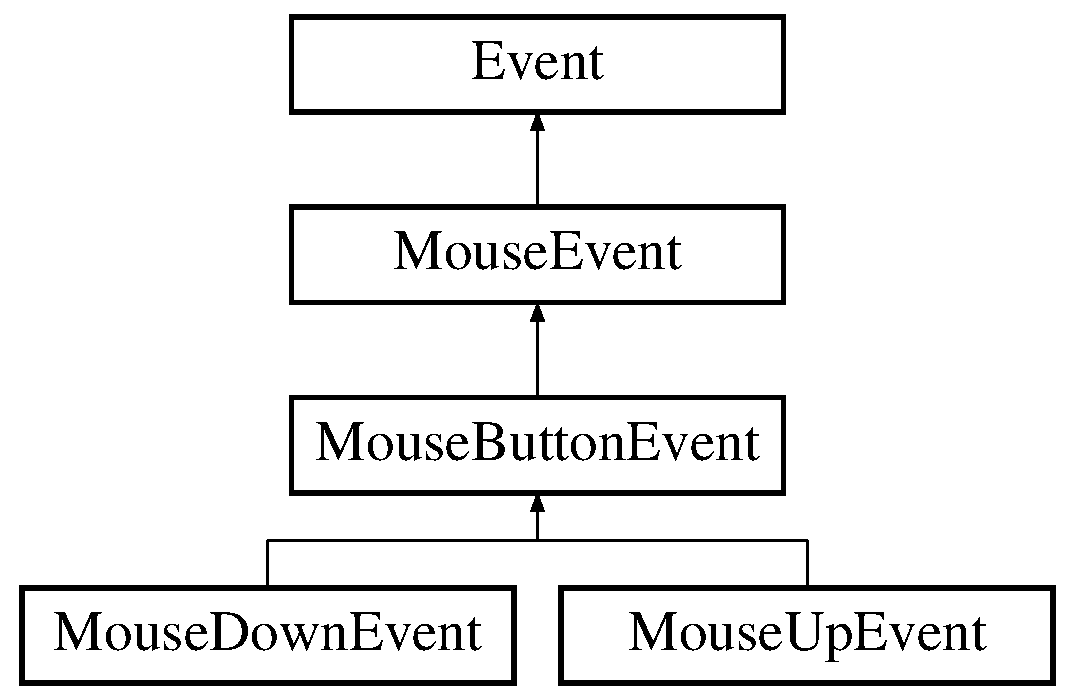
\includegraphics[height=4.000000cm]{structMouseButtonEvent}
\end{center}
\end{figure}
\subsection*{Public Attributes}
\begin{DoxyCompactItemize}
\item 
\hypertarget{structMouseButtonEvent_a91b45a7119f6cae5454b083b9c1d99c1}{const Mouse\+Button {\bfseries button}}\label{structMouseButtonEvent_a91b45a7119f6cae5454b083b9c1d99c1}

\end{DoxyCompactItemize}
\subsection*{Protected Member Functions}
\begin{DoxyCompactItemize}
\item 
\hypertarget{structMouseButtonEvent_a1dd634033a88534d5bedb2dee0f4299a}{{\bfseries Mouse\+Button\+Event} (\hyperlink{classEvent_a2abf13b5be49315e9e362af02029f058}{Type} type, float x, float y, float delta\+X, float delta\+Y, Mouse\+Button button)}\label{structMouseButtonEvent_a1dd634033a88534d5bedb2dee0f4299a}

\end{DoxyCompactItemize}
\subsection*{Additional Inherited Members}


\subsection{Detailed Description}
Write what the function does here. 


\begin{DoxyRetVals}{Return values}
{\em (variable)} & (description of variable) \\
\hline
\end{DoxyRetVals}


Definition at line 210 of file event.\+h.



The documentation for this struct was generated from the following file\+:\begin{DoxyCompactItemize}
\item 
event.\+h\end{DoxyCompactItemize}

\hypertarget{structMouseDownEvent}{\section{Mouse\+Down\+Event Struct Reference}
\label{structMouseDownEvent}\index{Mouse\+Down\+Event@{Mouse\+Down\+Event}}
}


Write what the function does here.  




{\ttfamily \#include $<$event.\+h$>$}

Inheritance diagram for Mouse\+Down\+Event\+:\begin{figure}[H]
\begin{center}
\leavevmode
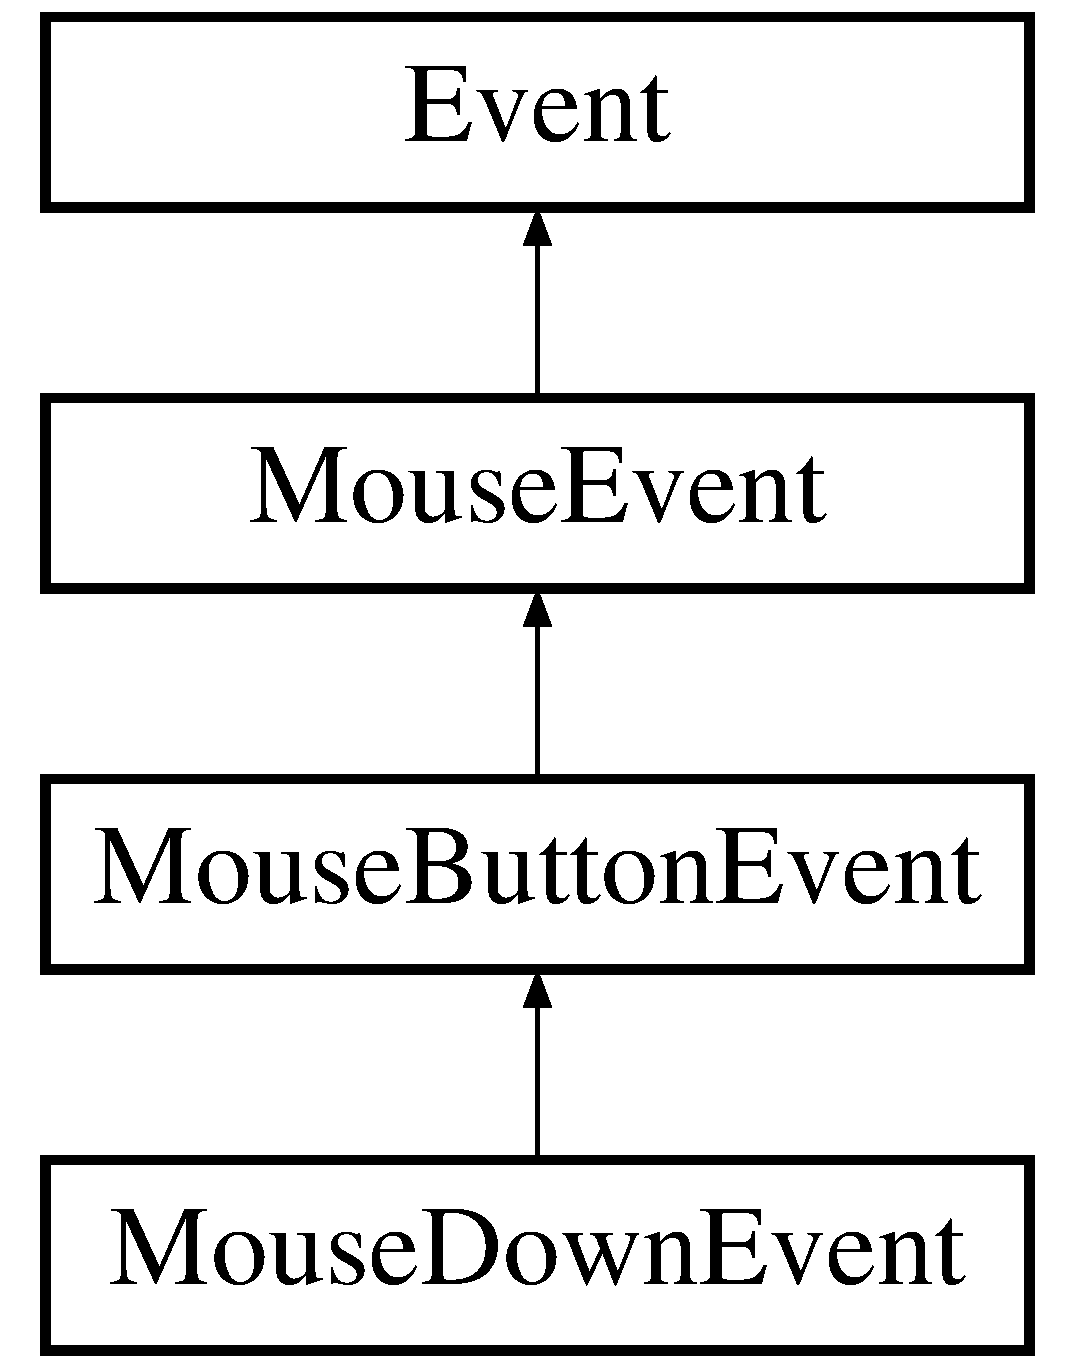
\includegraphics[height=4.000000cm]{structMouseDownEvent}
\end{center}
\end{figure}
\subsection*{Public Member Functions}
\begin{DoxyCompactItemize}
\item 
\hyperlink{structMouseDownEvent_a297d7e50d7363addef438a1a7e0981a8}{Mouse\+Down\+Event} (float x, float y, float delta\+X, float delta\+Y, Mouse\+Button button)
\begin{DoxyCompactList}\small\item\em Write what the function does here. \end{DoxyCompactList}\item 
virtual bool \hyperlink{structMouseDownEvent_a4c3d79107e6cef049a76089fd2b5b431}{dispatch} (shared\+\_\+ptr$<$ \hyperlink{structEventHandler}{Event\+Handler} $>$ event\+Handler) override
\begin{DoxyCompactList}\small\item\em Write what the function does here. \end{DoxyCompactList}\end{DoxyCompactItemize}
\subsection*{Additional Inherited Members}


\subsection{Detailed Description}
Write what the function does here. 

\begin{DoxyReturn}{Returns}

\end{DoxyReturn}


Definition at line 319 of file event.\+h.



\subsection{Constructor \& Destructor Documentation}
\hypertarget{structMouseDownEvent_a297d7e50d7363addef438a1a7e0981a8}{\index{Mouse\+Down\+Event@{Mouse\+Down\+Event}!Mouse\+Down\+Event@{Mouse\+Down\+Event}}
\index{Mouse\+Down\+Event@{Mouse\+Down\+Event}!Mouse\+Down\+Event@{Mouse\+Down\+Event}}
\subsubsection[{Mouse\+Down\+Event}]{\setlength{\rightskip}{0pt plus 5cm}Mouse\+Down\+Event\+::\+Mouse\+Down\+Event (
\begin{DoxyParamCaption}
\item[{float}]{x, }
\item[{float}]{y, }
\item[{float}]{delta\+X, }
\item[{float}]{delta\+Y, }
\item[{Mouse\+Button}]{button}
\end{DoxyParamCaption}
)\hspace{0.3cm}{\ttfamily [inline]}}}\label{structMouseDownEvent_a297d7e50d7363addef438a1a7e0981a8}


Write what the function does here. 


\begin{DoxyParams}{Parameters}
{\em Type\+\_\+\+Mouse\+Down} & \\
\hline
{\em x} & \\
\hline
{\em y} & \\
\hline
{\em delta\+X} & \\
\hline
{\em delta\+Y} & \\
\hline
{\em button} & \\
\hline
\end{DoxyParams}
\begin{DoxyReturn}{Returns}

\end{DoxyReturn}


Definition at line 321 of file event.\+h.


\begin{DoxyCode}
335         : \hyperlink{structMouseButtonEvent_a1dd634033a88534d5bedb2dee0f4299a}{MouseButtonEvent}(Type\_MouseDown, x, y, deltaX, deltaY, button)
336         \{
337         \}
\end{DoxyCode}


\subsection{Member Function Documentation}
\hypertarget{structMouseDownEvent_a4c3d79107e6cef049a76089fd2b5b431}{\index{Mouse\+Down\+Event@{Mouse\+Down\+Event}!dispatch@{dispatch}}
\index{dispatch@{dispatch}!Mouse\+Down\+Event@{Mouse\+Down\+Event}}
\subsubsection[{dispatch}]{\setlength{\rightskip}{0pt plus 5cm}virtual bool Mouse\+Down\+Event\+::dispatch (
\begin{DoxyParamCaption}
\item[{shared\+\_\+ptr$<$ {\bf Event\+Handler} $>$}]{event\+Handler}
\end{DoxyParamCaption}
)\hspace{0.3cm}{\ttfamily [inline]}, {\ttfamily [override]}, {\ttfamily [virtual]}}}\label{structMouseDownEvent_a4c3d79107e6cef049a76089fd2b5b431}


Write what the function does here. 


\begin{DoxyParams}{Parameters}
{\em event\+Handler} & \\
\hline
\end{DoxyParams}
\begin{DoxyReturn}{Returns}

\end{DoxyReturn}


Implements \hyperlink{classEvent}{Event}.



Definition at line 346 of file event.\+h.


\begin{DoxyCode}
347     \{
348         \textcolor{keywordflow}{return} eventHandler->handleMouseDown(*\textcolor{keyword}{this});
349     \}
\end{DoxyCode}


The documentation for this struct was generated from the following file\+:\begin{DoxyCompactItemize}
\item 
event.\+h\end{DoxyCompactItemize}

\hypertarget{classMouseEvent}{\section{Mouse\+Event Class Reference}
\label{classMouseEvent}\index{Mouse\+Event@{Mouse\+Event}}
}


Write what the function does here.  




{\ttfamily \#include $<$event.\+h$>$}

Inheritance diagram for Mouse\+Event\+:\begin{figure}[H]
\begin{center}
\leavevmode
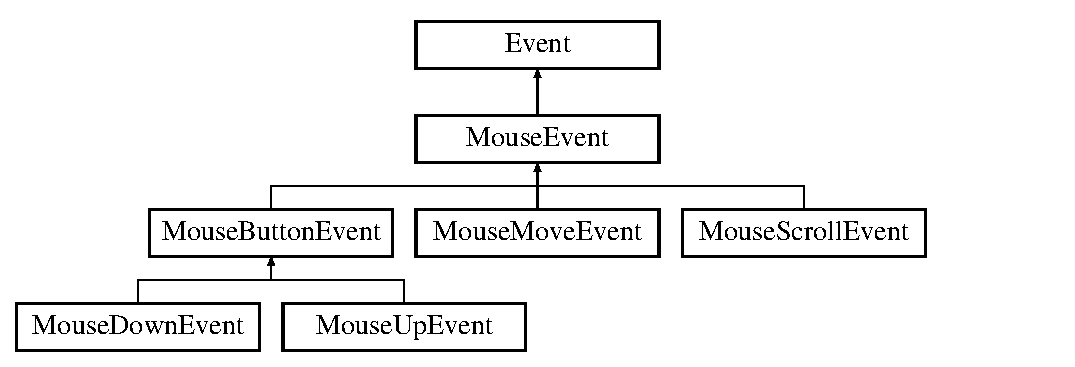
\includegraphics[height=4.000000cm]{classMouseEvent}
\end{center}
\end{figure}
\subsection*{Public Attributes}
\begin{DoxyCompactItemize}
\item 
\hypertarget{classMouseEvent_a32d72e73b9a01bac66b70c249939e8bd}{const float {\bfseries x}}\label{classMouseEvent_a32d72e73b9a01bac66b70c249939e8bd}

\item 
\hypertarget{classMouseEvent_a1153ae91317c28fbed841dda37f98ff1}{const float {\bfseries y}}\label{classMouseEvent_a1153ae91317c28fbed841dda37f98ff1}

\item 
\hypertarget{classMouseEvent_aadd4befdf86a50c7b13fb2e8d90f370c}{const float {\bfseries delta\+X}}\label{classMouseEvent_aadd4befdf86a50c7b13fb2e8d90f370c}

\item 
\hypertarget{classMouseEvent_a2a94fbca0cc7587701ead66279e87b47}{const float {\bfseries delta\+Y}}\label{classMouseEvent_a2a94fbca0cc7587701ead66279e87b47}

\end{DoxyCompactItemize}
\subsection*{Protected Member Functions}
\begin{DoxyCompactItemize}
\item 
\hypertarget{classMouseEvent_a38e3202976fe08a74713bbb3326004c6}{{\bfseries Mouse\+Event} (\hyperlink{classEvent_a2abf13b5be49315e9e362af02029f058}{Type} type, float x, float y, float delta\+X, float delta\+Y)}\label{classMouseEvent_a38e3202976fe08a74713bbb3326004c6}

\end{DoxyCompactItemize}
\subsection*{Additional Inherited Members}


\subsection{Detailed Description}
Write what the function does here. 

\begin{DoxyReturn}{Returns}

\end{DoxyReturn}


Definition at line 72 of file event.\+h.



The documentation for this class was generated from the following file\+:\begin{DoxyCompactItemize}
\item 
event.\+h\end{DoxyCompactItemize}

\hypertarget{structMouseMoveEvent}{\section{Mouse\+Move\+Event Struct Reference}
\label{structMouseMoveEvent}\index{Mouse\+Move\+Event@{Mouse\+Move\+Event}}
}


Write what the function does here.  




{\ttfamily \#include $<$event.\+h$>$}

Inheritance diagram for Mouse\+Move\+Event\+:\begin{figure}[H]
\begin{center}
\leavevmode
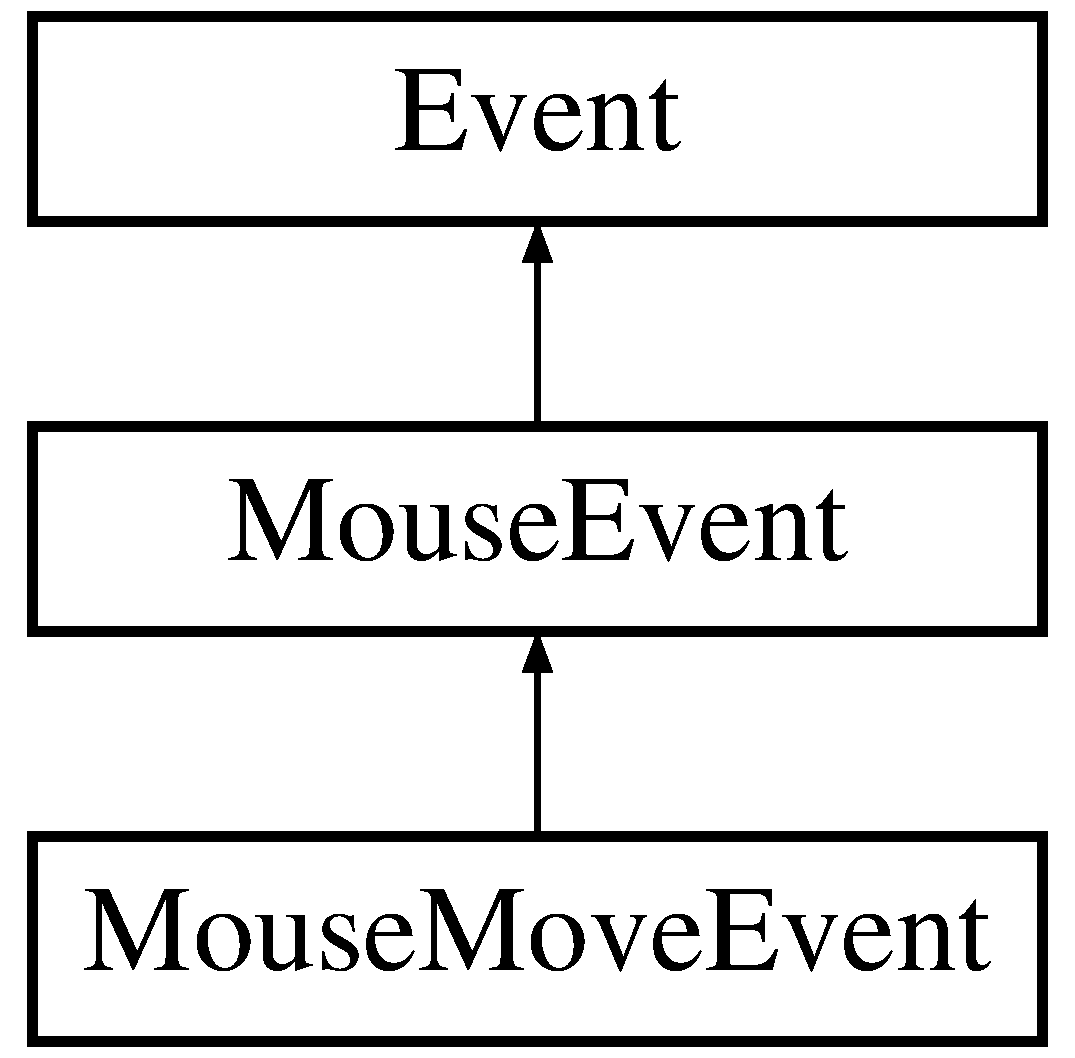
\includegraphics[height=3.000000cm]{structMouseMoveEvent}
\end{center}
\end{figure}
\subsection*{Public Member Functions}
\begin{DoxyCompactItemize}
\item 
\hypertarget{structMouseMoveEvent_abf421414902d34aa2d9435cc485fc4c8}{{\bfseries Mouse\+Move\+Event} (float x, float y, float delta\+X, float delta\+Y)}\label{structMouseMoveEvent_abf421414902d34aa2d9435cc485fc4c8}

\item 
virtual bool \hyperlink{structMouseMoveEvent_a2718ebd4f6f40d533773e59530372d62}{dispatch} (shared\+\_\+ptr$<$ \hyperlink{structEventHandler}{Event\+Handler} $>$ event\+Handler) override
\begin{DoxyCompactList}\small\item\em Write what the function does here. \end{DoxyCompactList}\end{DoxyCompactItemize}
\subsection*{Additional Inherited Members}


\subsection{Detailed Description}
Write what the function does here. 


\begin{DoxyRetVals}{Return values}
{\em (variable)} & (description of variable) \\
\hline
\end{DoxyRetVals}


Definition at line 292 of file event.\+h.



\subsection{Member Function Documentation}
\hypertarget{structMouseMoveEvent_a2718ebd4f6f40d533773e59530372d62}{\index{Mouse\+Move\+Event@{Mouse\+Move\+Event}!dispatch@{dispatch}}
\index{dispatch@{dispatch}!Mouse\+Move\+Event@{Mouse\+Move\+Event}}
\subsubsection[{dispatch}]{\setlength{\rightskip}{0pt plus 5cm}virtual bool Mouse\+Move\+Event\+::dispatch (
\begin{DoxyParamCaption}
\item[{shared\+\_\+ptr$<$ {\bf Event\+Handler} $>$}]{event\+Handler}
\end{DoxyParamCaption}
)\hspace{0.3cm}{\ttfamily [inline]}, {\ttfamily [override]}, {\ttfamily [virtual]}}}\label{structMouseMoveEvent_a2718ebd4f6f40d533773e59530372d62}


Write what the function does here. 


\begin{DoxyParams}{Parameters}
{\em event\+Handler} & \\
\hline
\end{DoxyParams}

\begin{DoxyRetVals}{Return values}
{\em (variable)} & (description of variable) \\
\hline
\end{DoxyRetVals}


Implements \hyperlink{classEvent}{Event}.



Definition at line 306 of file event.\+h.


\begin{DoxyCode}
307     \{
308         \textcolor{keywordflow}{return} eventHandler->handleMouseMove(*\textcolor{keyword}{this});
309     \}
\end{DoxyCode}


The documentation for this struct was generated from the following file\+:\begin{DoxyCompactItemize}
\item 
event.\+h\end{DoxyCompactItemize}

\hypertarget{structMouseScrollEvent}{\section{Mouse\+Scroll\+Event Struct Reference}
\label{structMouseScrollEvent}\index{Mouse\+Scroll\+Event@{Mouse\+Scroll\+Event}}
}


Write what the function does here.  




{\ttfamily \#include $<$event.\+h$>$}

Inheritance diagram for Mouse\+Scroll\+Event\+:\begin{figure}[H]
\begin{center}
\leavevmode
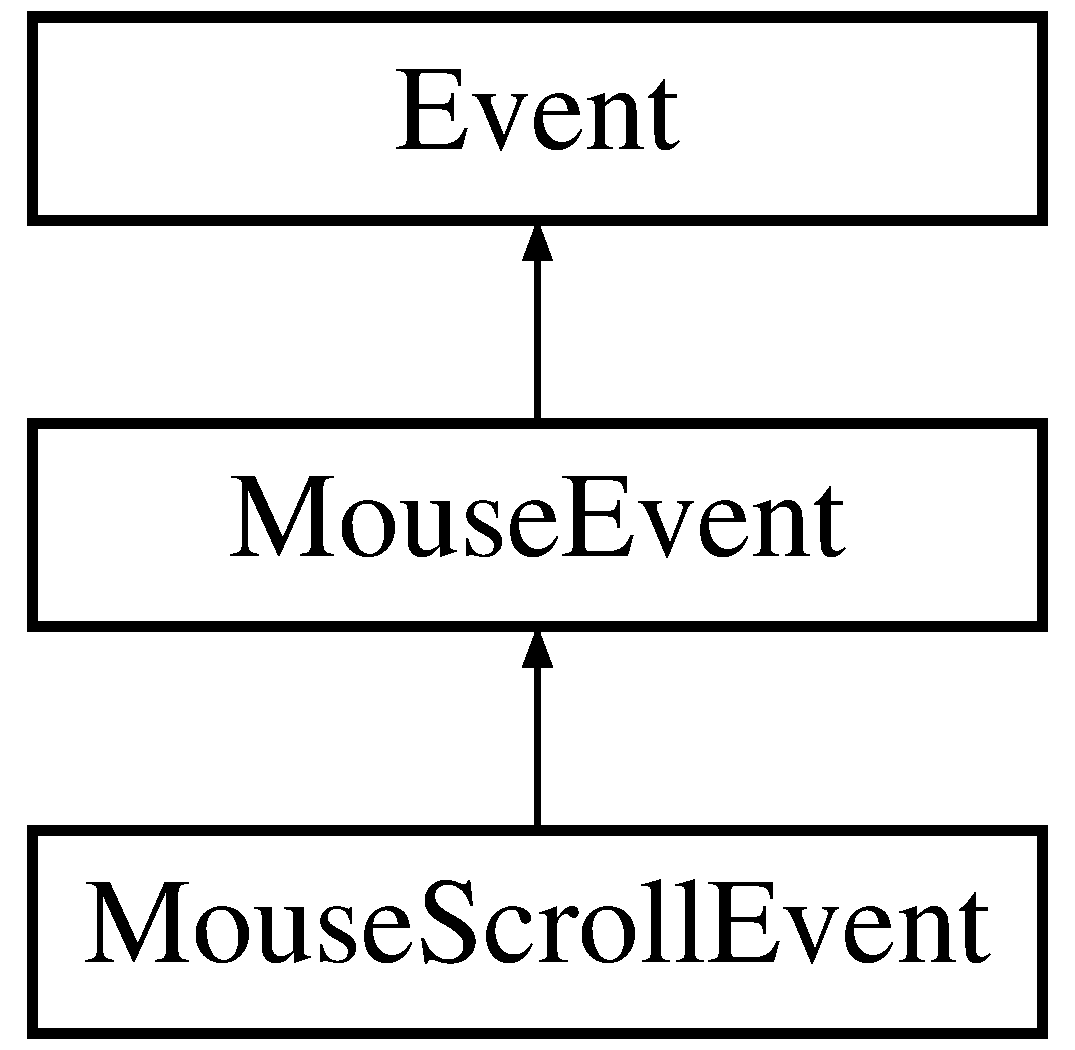
\includegraphics[height=3.000000cm]{structMouseScrollEvent}
\end{center}
\end{figure}
\subsection*{Public Member Functions}
\begin{DoxyCompactItemize}
\item 
\hypertarget{structMouseScrollEvent_a7fffc52d48bef83bcf2aea47734c3fca}{{\bfseries Mouse\+Scroll\+Event} (float x, float y, float delta\+X, float delta\+Y, int scroll\+X, int scroll\+Y)}\label{structMouseScrollEvent_a7fffc52d48bef83bcf2aea47734c3fca}

\item 
virtual bool \hyperlink{structMouseScrollEvent_acaa9673a50db8c33dd1cdbf1c5da2816}{dispatch} (shared\+\_\+ptr$<$ \hyperlink{structEventHandler}{Event\+Handler} $>$ event\+Handler) override
\begin{DoxyCompactList}\small\item\em Write what the function does here. \end{DoxyCompactList}\end{DoxyCompactItemize}
\subsection*{Public Attributes}
\begin{DoxyCompactItemize}
\item 
\hypertarget{structMouseScrollEvent_aed934d011f9c2fd1cd63f1b53bec598d}{const int {\bfseries scroll\+X}}\label{structMouseScrollEvent_aed934d011f9c2fd1cd63f1b53bec598d}

\item 
\hypertarget{structMouseScrollEvent_aefa811ca1ad2b3ef22c4423241e3ae40}{const int {\bfseries scroll\+Y}}\label{structMouseScrollEvent_aefa811ca1ad2b3ef22c4423241e3ae40}

\end{DoxyCompactItemize}
\subsection*{Additional Inherited Members}


\subsection{Detailed Description}
Write what the function does here. 

\begin{DoxyReturn}{Returns}

\end{DoxyReturn}


Definition at line 317 of file event.\+h.



\subsection{Member Function Documentation}
\hypertarget{structMouseScrollEvent_acaa9673a50db8c33dd1cdbf1c5da2816}{\index{Mouse\+Scroll\+Event@{Mouse\+Scroll\+Event}!dispatch@{dispatch}}
\index{dispatch@{dispatch}!Mouse\+Scroll\+Event@{Mouse\+Scroll\+Event}}
\subsubsection[{dispatch}]{\setlength{\rightskip}{0pt plus 5cm}virtual bool Mouse\+Scroll\+Event\+::dispatch (
\begin{DoxyParamCaption}
\item[{shared\+\_\+ptr$<$ {\bf Event\+Handler} $>$}]{event\+Handler}
\end{DoxyParamCaption}
)\hspace{0.3cm}{\ttfamily [inline]}, {\ttfamily [override]}, {\ttfamily [virtual]}}}\label{structMouseScrollEvent_acaa9673a50db8c33dd1cdbf1c5da2816}


Write what the function does here. 


\begin{DoxyParams}{Parameters}
{\em event\+Handler} & \\
\hline
\end{DoxyParams}
\begin{DoxyReturn}{Returns}

\end{DoxyReturn}


Implements \hyperlink{classEvent}{Event}.



Definition at line 332 of file event.\+h.


\begin{DoxyCode}
333     \{
334         \textcolor{keywordflow}{return} eventHandler->handleMouseScroll(*\textcolor{keyword}{this});
335     \}
\end{DoxyCode}


The documentation for this struct was generated from the following file\+:\begin{DoxyCompactItemize}
\item 
event.\+h\end{DoxyCompactItemize}

\hypertarget{structMouseUpEvent}{\section{Mouse\+Up\+Event Struct Reference}
\label{structMouseUpEvent}\index{Mouse\+Up\+Event@{Mouse\+Up\+Event}}
}


Write what the function does here.  




{\ttfamily \#include $<$event.\+h$>$}

Inheritance diagram for Mouse\+Up\+Event\+:\begin{figure}[H]
\begin{center}
\leavevmode
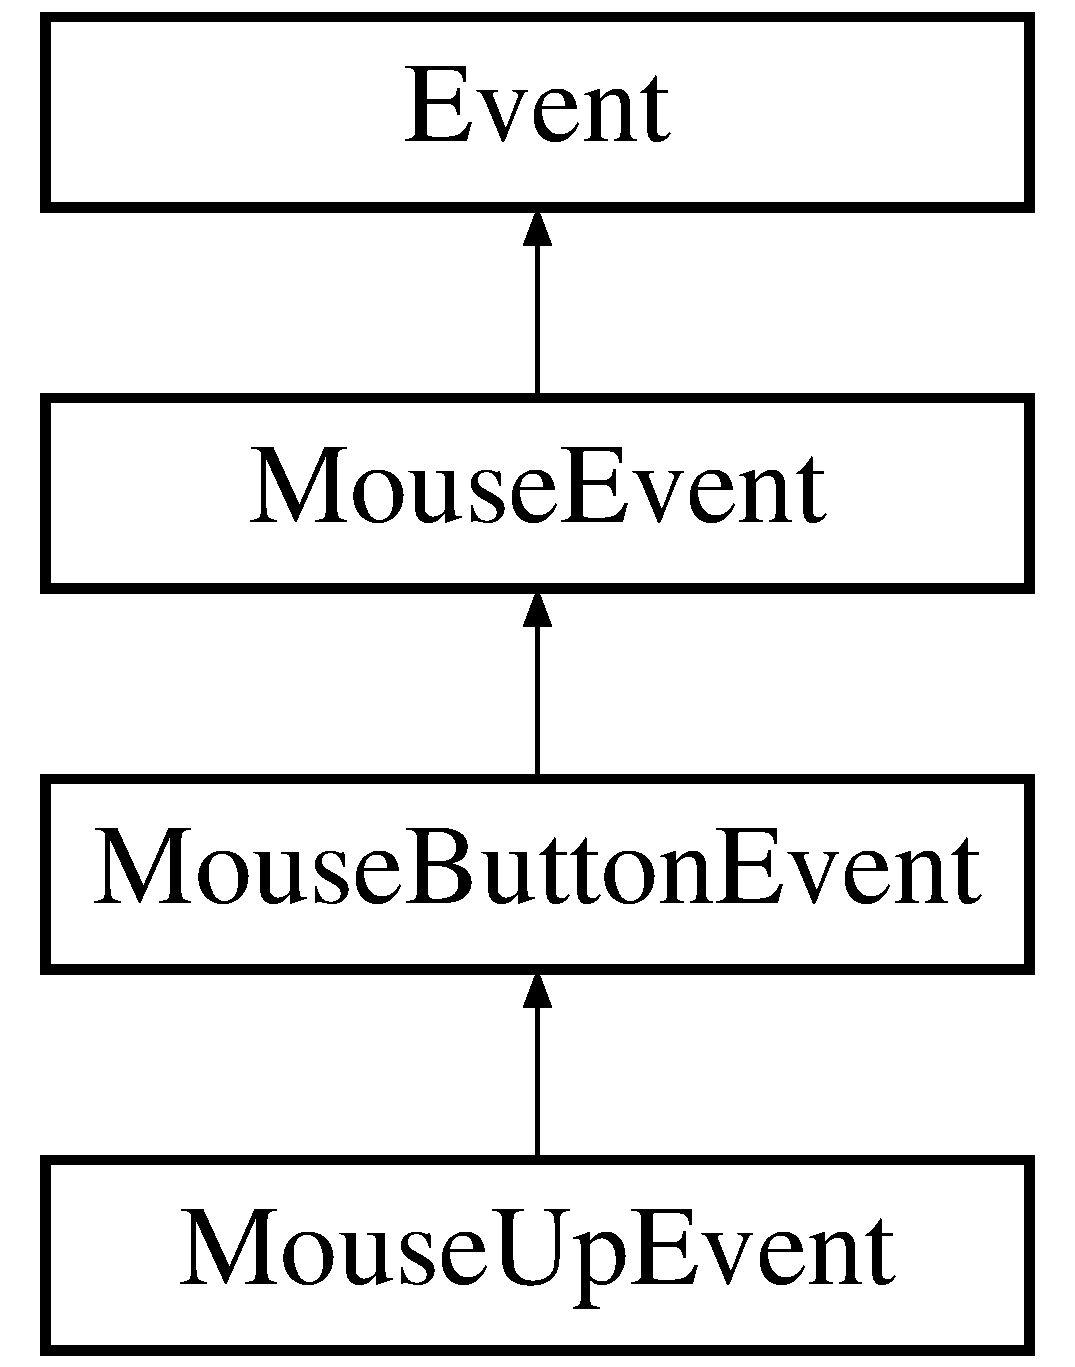
\includegraphics[height=4.000000cm]{structMouseUpEvent}
\end{center}
\end{figure}
\subsection*{Public Member Functions}
\begin{DoxyCompactItemize}
\item 
\hyperlink{structMouseUpEvent_ac1395cedfc2ab584976e41450cbdeab9}{Mouse\+Up\+Event} (float x, float y, float delta\+X, float delta\+Y, Mouse\+Button button)
\begin{DoxyCompactList}\small\item\em Write what the function does here. \end{DoxyCompactList}\item 
virtual bool \hyperlink{structMouseUpEvent_a013d0f9ff763239e909347e7624bfa04}{dispatch} (shared\+\_\+ptr$<$ \hyperlink{structEventHandler}{Event\+Handler} $>$ event\+Handler) override
\begin{DoxyCompactList}\small\item\em Write what the function does here. \end{DoxyCompactList}\end{DoxyCompactItemize}
\subsection*{Additional Inherited Members}


\subsection{Detailed Description}
Write what the function does here. 


\begin{DoxyRetVals}{Return values}
{\em (variable)} & (description of variable) \\
\hline
\end{DoxyRetVals}


Definition at line 225 of file event.\+h.



\subsection{Constructor \& Destructor Documentation}
\hypertarget{structMouseUpEvent_ac1395cedfc2ab584976e41450cbdeab9}{\index{Mouse\+Up\+Event@{Mouse\+Up\+Event}!Mouse\+Up\+Event@{Mouse\+Up\+Event}}
\index{Mouse\+Up\+Event@{Mouse\+Up\+Event}!Mouse\+Up\+Event@{Mouse\+Up\+Event}}
\subsubsection[{Mouse\+Up\+Event}]{\setlength{\rightskip}{0pt plus 5cm}Mouse\+Up\+Event\+::\+Mouse\+Up\+Event (
\begin{DoxyParamCaption}
\item[{float}]{x, }
\item[{float}]{y, }
\item[{float}]{delta\+X, }
\item[{float}]{delta\+Y, }
\item[{Mouse\+Button}]{button}
\end{DoxyParamCaption}
)\hspace{0.3cm}{\ttfamily [inline]}}}\label{structMouseUpEvent_ac1395cedfc2ab584976e41450cbdeab9}


Write what the function does here. 


\begin{DoxyParams}{Parameters}
{\em x} & \\
\hline
{\em y} & \\
\hline
{\em delta\+X} & \\
\hline
{\em delta\+Y} & \\
\hline
{\em button} & \\
\hline
{\em Type\+\_\+\+Mouse\+Up} & \\
\hline
{\em x} & \\
\hline
{\em y} & \\
\hline
{\em delta\+X} & \\
\hline
{\em delta\+Y} & \\
\hline
{\em button} & \\
\hline
\end{DoxyParams}

\begin{DoxyRetVals}{Return values}
{\em (variable)} & (description of variable) \\
\hline
\end{DoxyRetVals}


Definition at line 245 of file event.\+h.


\begin{DoxyCode}
245                                                                                    : 
      \hyperlink{structMouseButtonEvent}{MouseButtonEvent}(Type\_MouseUp, x, y, deltaX, deltaY, button)
246     \{
247     \}
\end{DoxyCode}


\subsection{Member Function Documentation}
\hypertarget{structMouseUpEvent_a013d0f9ff763239e909347e7624bfa04}{\index{Mouse\+Up\+Event@{Mouse\+Up\+Event}!dispatch@{dispatch}}
\index{dispatch@{dispatch}!Mouse\+Up\+Event@{Mouse\+Up\+Event}}
\subsubsection[{dispatch}]{\setlength{\rightskip}{0pt plus 5cm}virtual bool Mouse\+Up\+Event\+::dispatch (
\begin{DoxyParamCaption}
\item[{shared\+\_\+ptr$<$ {\bf Event\+Handler} $>$}]{event\+Handler}
\end{DoxyParamCaption}
)\hspace{0.3cm}{\ttfamily [inline]}, {\ttfamily [override]}, {\ttfamily [virtual]}}}\label{structMouseUpEvent_a013d0f9ff763239e909347e7624bfa04}


Write what the function does here. 


\begin{DoxyParams}{Parameters}
{\em event\+Handler} & \\
\hline
\end{DoxyParams}

\begin{DoxyRetVals}{Return values}
{\em (variable)} & (description of variable) \\
\hline
\end{DoxyRetVals}


Implements \hyperlink{classEvent}{Event}.



Definition at line 256 of file event.\+h.


\begin{DoxyCode}
257     \{
258         \textcolor{keywordflow}{return} eventHandler->handleMouseUp(*\textcolor{keyword}{this});
259     \}
\end{DoxyCode}


The documentation for this struct was generated from the following file\+:\begin{DoxyCompactItemize}
\item 
event.\+h\end{DoxyCompactItemize}

\hypertarget{structNativeWindowFactory}{\section{Native\+Window\+Factory Struct Reference}
\label{structNativeWindowFactory}\index{Native\+Window\+Factory@{Native\+Window\+Factory}}
}
\subsection*{Public Attributes}
\begin{DoxyCompactItemize}
\item 
\hypertarget{structNativeWindowFactory_a060b40251dfcd62a39812b8e971f11fe}{const char $\ast$ {\bfseries tag}}\label{structNativeWindowFactory_a060b40251dfcd62a39812b8e971f11fe}

\item 
\hypertarget{structNativeWindowFactory_ab53b8a66d49db2f46440a4d4d5482685}{void $\ast$($\ast$ {\bfseries Create\+Native\+Window} )(int w, int h)}\label{structNativeWindowFactory_ab53b8a66d49db2f46440a4d4d5482685}

\item 
\hypertarget{structNativeWindowFactory_a31ccd4ce1039bd7b6eae7302b2d558eb}{void($\ast$ {\bfseries Destroy\+Native\+Window} )(void $\ast$window)}\label{structNativeWindowFactory_a31ccd4ce1039bd7b6eae7302b2d558eb}

\end{DoxyCompactItemize}


\subsection{Detailed Description}


Definition at line 22 of file testnative.\+h.



The documentation for this struct was generated from the following file\+:\begin{DoxyCompactItemize}
\item 
S\+D\+L2-\/2.\+0.\+3/test/testnative.\+h\end{DoxyCompactItemize}

\hypertarget{classNetworkConnection}{\section{Network\+Connection Class Reference}
\label{classNetworkConnection}\index{Network\+Connection@{Network\+Connection}}
}


Write what the function does here.  




{\ttfamily \#include $<$network.\+h$>$}

Inheritance diagram for Network\+Connection\+:\begin{figure}[H]
\begin{center}
\leavevmode
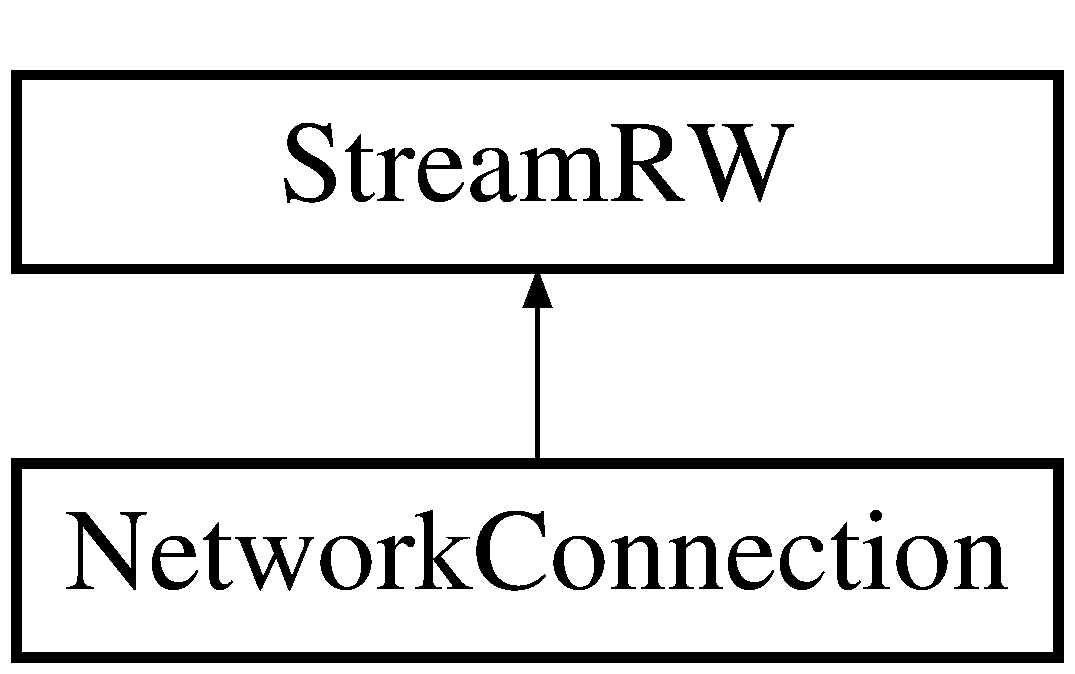
\includegraphics[height=2.000000cm]{classNetworkConnection}
\end{center}
\end{figure}
\subsection*{Public Member Functions}
\begin{DoxyCompactItemize}
\item 
\hypertarget{classNetworkConnection_a78733e203c2aef9a0cb1538476c637d7}{{\bfseries Network\+Connection} (wstring url, uint16\+\_\+t port)}\label{classNetworkConnection_a78733e203c2aef9a0cb1538476c637d7}

\item 
shared\+\_\+ptr$<$ \hyperlink{classReader}{Reader} $>$ \hyperlink{classNetworkConnection_a3cd959362a6b007ad005f330463c2216}{preader} () override
\begin{DoxyCompactList}\small\item\em Write what the function does here. \end{DoxyCompactList}\item 
shared\+\_\+ptr$<$ \hyperlink{classWriter}{Writer} $>$ \hyperlink{classNetworkConnection_a2cc73fa5d5c9b4cf74579946dc136b5a}{pwriter} () override
\begin{DoxyCompactList}\small\item\em Write what the function does here. \end{DoxyCompactList}\end{DoxyCompactItemize}
\subsection*{Private Member Functions}
\begin{DoxyCompactItemize}
\item 
\hyperlink{classNetworkConnection_a9a07574433d99140bae5f156c1985394}{Network\+Connection} (int read\+Fd, int write\+Fd)
\begin{DoxyCompactList}\small\item\em Write what the function does here. \end{DoxyCompactList}\end{DoxyCompactItemize}
\subsection*{Private Attributes}
\begin{DoxyCompactItemize}
\item 
\hypertarget{classNetworkConnection_af4802dedf4ab9533305501fd2b37a77c}{shared\+\_\+ptr$<$ \hyperlink{classReader}{Reader} $>$ {\bfseries reader\+Internal}}\label{classNetworkConnection_af4802dedf4ab9533305501fd2b37a77c}

\item 
\hypertarget{classNetworkConnection_adcad1f46ad36fe40b3f45ed12c6369e5}{shared\+\_\+ptr$<$ \hyperlink{classWriter}{Writer} $>$ {\bfseries writer\+Internal}}\label{classNetworkConnection_adcad1f46ad36fe40b3f45ed12c6369e5}

\end{DoxyCompactItemize}
\subsection*{Friends}
\begin{DoxyCompactItemize}
\item 
\hypertarget{classNetworkConnection_a9aeeeda70dbfefcf76c52db5f76274ab}{class {\bfseries Network\+Server}}\label{classNetworkConnection_a9aeeeda70dbfefcf76c52db5f76274ab}

\end{DoxyCompactItemize}


\subsection{Detailed Description}
Write what the function does here. 

\begin{DoxyReturn}{Returns}

\end{DoxyReturn}


Definition at line 33 of file network.\+h.



\subsection{Constructor \& Destructor Documentation}
\hypertarget{classNetworkConnection_a9a07574433d99140bae5f156c1985394}{\index{Network\+Connection@{Network\+Connection}!Network\+Connection@{Network\+Connection}}
\index{Network\+Connection@{Network\+Connection}!Network\+Connection@{Network\+Connection}}
\subsubsection[{Network\+Connection}]{\setlength{\rightskip}{0pt plus 5cm}Network\+Connection\+::\+Network\+Connection (
\begin{DoxyParamCaption}
\item[{int}]{read\+Fd, }
\item[{int}]{write\+Fd}
\end{DoxyParamCaption}
)\hspace{0.3cm}{\ttfamily [inline]}, {\ttfamily [private]}}}\label{classNetworkConnection_a9a07574433d99140bae5f156c1985394}


Write what the function does here. 


\begin{DoxyParams}{Parameters}
{\em read\+Fd} & \\
\hline
{\em write\+Fd} & \\
\hline
\end{DoxyParams}
\begin{DoxyReturn}{Returns}

\end{DoxyReturn}


Definition at line 39 of file network.\+h.


\begin{DoxyCode}
49         : readerInternal(\textcolor{keyword}{new} \hyperlink{classFileReader}{FileReader}(fdopen(readFd, \textcolor{stringliteral}{"r"}))), writerInternal(\textcolor{keyword}{new} FileWriter(
      fdopen(writeFd, \textcolor{stringliteral}{"w"})))
50         \{
51         \}
\end{DoxyCode}


\subsection{Member Function Documentation}
\hypertarget{classNetworkConnection_a3cd959362a6b007ad005f330463c2216}{\index{Network\+Connection@{Network\+Connection}!preader@{preader}}
\index{preader@{preader}!Network\+Connection@{Network\+Connection}}
\subsubsection[{preader}]{\setlength{\rightskip}{0pt plus 5cm}shared\+\_\+ptr$<${\bf Reader}$>$ Network\+Connection\+::preader (
\begin{DoxyParamCaption}
{}
\end{DoxyParamCaption}
)\hspace{0.3cm}{\ttfamily [inline]}, {\ttfamily [override]}}}\label{classNetworkConnection_a3cd959362a6b007ad005f330463c2216}


Write what the function does here. 

\begin{DoxyReturn}{Returns}

\end{DoxyReturn}


Definition at line 60 of file network.\+h.


\begin{DoxyCode}
61     \{
62         \textcolor{keywordflow}{return} readerInternal;
63     \}
\end{DoxyCode}
\hypertarget{classNetworkConnection_a2cc73fa5d5c9b4cf74579946dc136b5a}{\index{Network\+Connection@{Network\+Connection}!pwriter@{pwriter}}
\index{pwriter@{pwriter}!Network\+Connection@{Network\+Connection}}
\subsubsection[{pwriter}]{\setlength{\rightskip}{0pt plus 5cm}shared\+\_\+ptr$<${\bf Writer}$>$ Network\+Connection\+::pwriter (
\begin{DoxyParamCaption}
{}
\end{DoxyParamCaption}
)\hspace{0.3cm}{\ttfamily [inline]}, {\ttfamily [override]}}}\label{classNetworkConnection_a2cc73fa5d5c9b4cf74579946dc136b5a}


Write what the function does here. 

\begin{DoxyReturn}{Returns}

\end{DoxyReturn}


Definition at line 70 of file network.\+h.


\begin{DoxyCode}
71     \{
72         \textcolor{keywordflow}{return} writerInternal;
73     \}
\end{DoxyCode}


The documentation for this class was generated from the following files\+:\begin{DoxyCompactItemize}
\item 
network.\+h\item 
network.\+cpp\end{DoxyCompactItemize}

\hypertarget{classNetworkException}{\section{Network\+Exception Class Reference}
\label{classNetworkException}\index{Network\+Exception@{Network\+Exception}}
}


Write what the function does here.  




{\ttfamily \#include $<$network.\+h$>$}

Inheritance diagram for Network\+Exception\+:\begin{figure}[H]
\begin{center}
\leavevmode
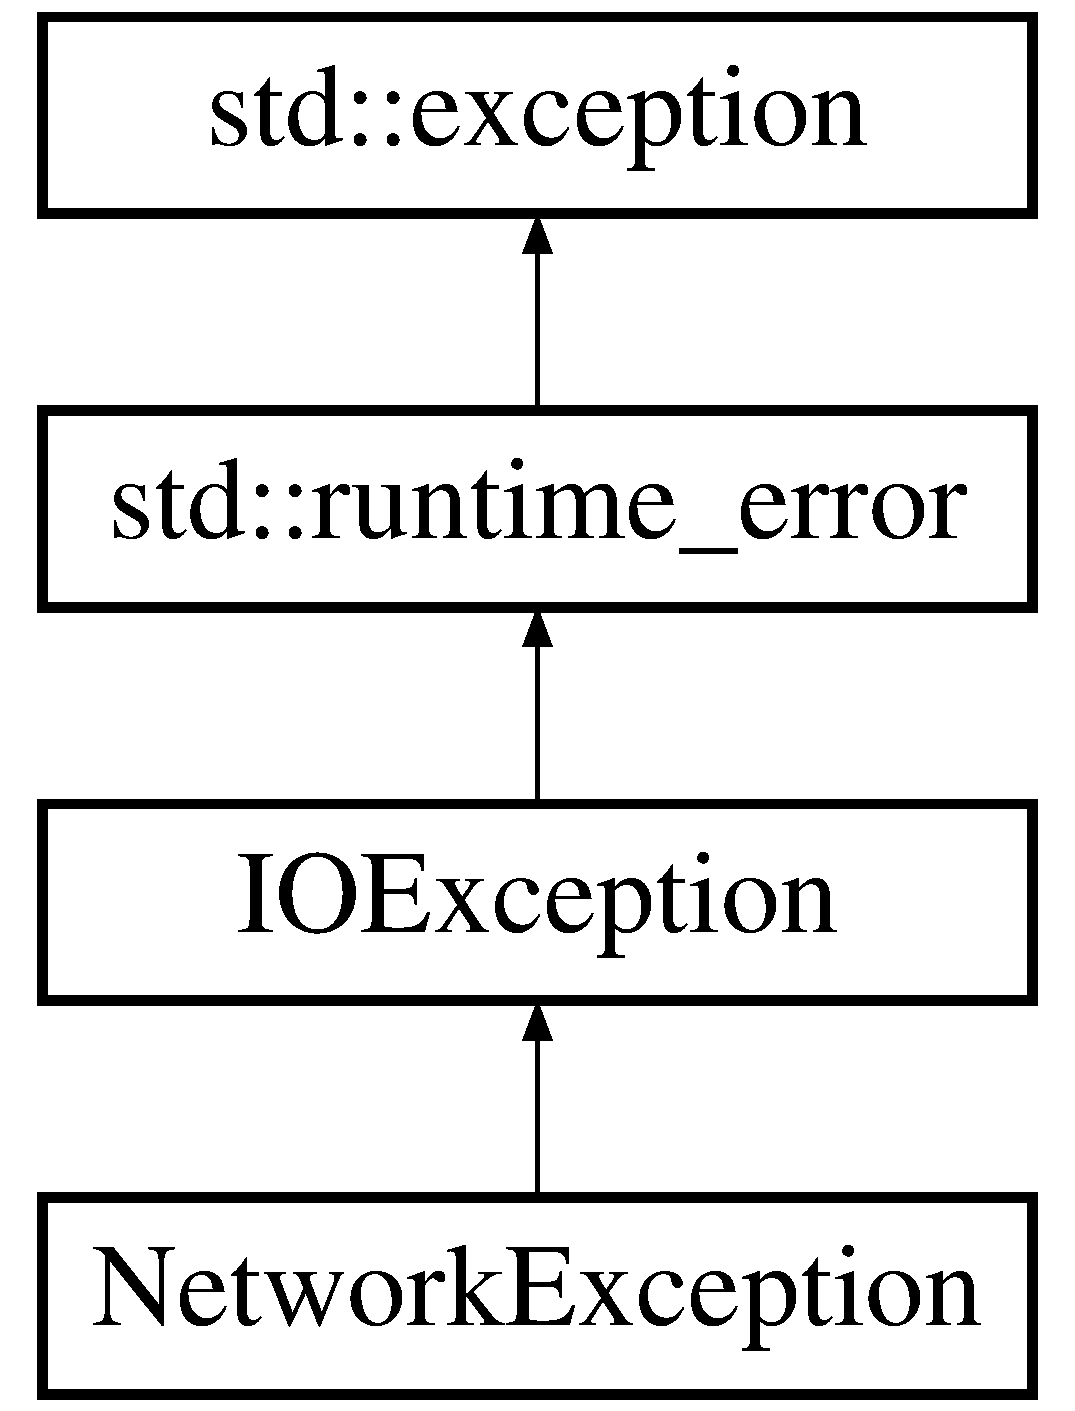
\includegraphics[height=4.000000cm]{classNetworkException}
\end{center}
\end{figure}
\subsection*{Public Member Functions}
\begin{DoxyCompactItemize}
\item 
\hyperlink{classNetworkException_a7b2fde9c75da04d6a3d9e5bb332594ac}{Network\+Exception} (string msg)
\begin{DoxyCompactList}\small\item\em Write what the function does here. \end{DoxyCompactList}\end{DoxyCompactItemize}


\subsection{Detailed Description}
Write what the function does here. 

\begin{DoxyReturn}{Returns}

\end{DoxyReturn}


Definition at line 11 of file network.\+h.



\subsection{Constructor \& Destructor Documentation}
\hypertarget{classNetworkException_a7b2fde9c75da04d6a3d9e5bb332594ac}{\index{Network\+Exception@{Network\+Exception}!Network\+Exception@{Network\+Exception}}
\index{Network\+Exception@{Network\+Exception}!Network\+Exception@{Network\+Exception}}
\subsubsection[{Network\+Exception}]{\setlength{\rightskip}{0pt plus 5cm}Network\+Exception\+::\+Network\+Exception (
\begin{DoxyParamCaption}
\item[{string}]{msg}
\end{DoxyParamCaption}
)\hspace{0.3cm}{\ttfamily [inline]}, {\ttfamily [explicit]}}}\label{classNetworkException_a7b2fde9c75da04d6a3d9e5bb332594ac}


Write what the function does here. 


\begin{DoxyParams}{Parameters}
{\em msg} & \\
\hline
\end{DoxyParams}
\begin{DoxyReturn}{Returns}

\end{DoxyReturn}


Definition at line 14 of file network.\+h.


\begin{DoxyCode}
23             : \hyperlink{classIOException_a73fcf78b1b5820aa158680e896f0b983}{IOException}(msg)
24             \{
25             \}
\end{DoxyCode}


The documentation for this class was generated from the following file\+:\begin{DoxyCompactItemize}
\item 
network.\+h\end{DoxyCompactItemize}

\hypertarget{classNetworkServer}{\section{Network\+Server Class Reference}
\label{classNetworkServer}\index{Network\+Server@{Network\+Server}}
}


Write what the function does here.  




{\ttfamily \#include $<$network.\+h$>$}

Inheritance diagram for Network\+Server\+:\begin{figure}[H]
\begin{center}
\leavevmode
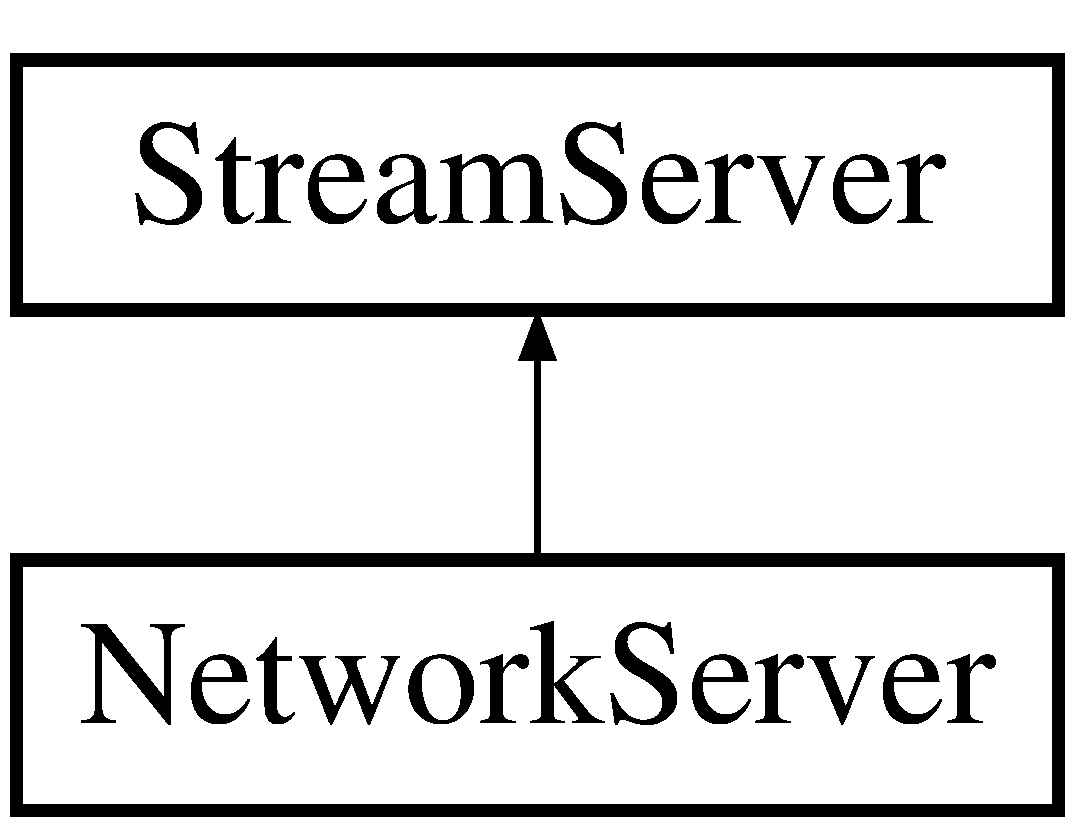
\includegraphics[height=2.000000cm]{classNetworkServer}
\end{center}
\end{figure}
\subsection*{Public Member Functions}
\begin{DoxyCompactItemize}
\item 
\hypertarget{classNetworkServer_abf7631e55048fc28a4edcaebd7f88e2e}{{\bfseries Network\+Server} (uint16\+\_\+t port)}\label{classNetworkServer_abf7631e55048fc28a4edcaebd7f88e2e}

\item 
\hypertarget{classNetworkServer_a88d231dddf7c327f5e68686e1874001a}{shared\+\_\+ptr$<$ Stream\+R\+W $>$ {\bfseries accept} () override}\label{classNetworkServer_a88d231dddf7c327f5e68686e1874001a}

\end{DoxyCompactItemize}
\subsection*{Private Member Functions}
\begin{DoxyCompactItemize}
\item 
\hypertarget{classNetworkServer_afa83400cf119ab3f619919a006f0e0ba}{{\bfseries Network\+Server} (const \hyperlink{classNetworkServer}{Network\+Server} \&)=delete}\label{classNetworkServer_afa83400cf119ab3f619919a006f0e0ba}

\item 
\hypertarget{classNetworkServer_ae7669127d3dbd8e027fcf15cca9e5859}{const \hyperlink{classNetworkServer}{Network\+Server} \& {\bfseries operator=} (const \hyperlink{classNetworkServer}{Network\+Server} \&)=delete}\label{classNetworkServer_ae7669127d3dbd8e027fcf15cca9e5859}

\end{DoxyCompactItemize}
\subsection*{Private Attributes}
\begin{DoxyCompactItemize}
\item 
\hypertarget{classNetworkServer_a3a4cbba07f7c425a9147f8a21b714e7f}{int {\bfseries fd}}\label{classNetworkServer_a3a4cbba07f7c425a9147f8a21b714e7f}

\end{DoxyCompactItemize}


\subsection{Detailed Description}
Write what the function does here. 

\begin{DoxyReturn}{Returns}

\end{DoxyReturn}


Definition at line 64 of file network.\+h.



The documentation for this class was generated from the following files\+:\begin{DoxyCompactItemize}
\item 
network.\+h\item 
network.\+cpp\end{DoxyCompactItemize}

\hypertarget{structgraph_1_1Node}{\section{graph$<$ N\+T, E\+T $>$\+:\+:Node Struct Reference}
\label{structgraph_1_1Node}\index{graph$<$ N\+T, E\+T $>$\+::\+Node@{graph$<$ N\+T, E\+T $>$\+::\+Node}}
}


Write what the function does here.  


\subsection*{Public Member Functions}
\begin{DoxyCompactItemize}
\item 
\hypertarget{structgraph_1_1Node_a2ea59c8e60a21337707a4724ec2187c3}{{\bfseries Node} (int index, const N\+T \&data)}\label{structgraph_1_1Node_a2ea59c8e60a21337707a4724ec2187c3}

\item 
\hypertarget{structgraph_1_1Node_a00ae7db8b8befe0e81b08dc6da311ce4}{{\bfseries Node} (int index, N\+T \&\&data)}\label{structgraph_1_1Node_a00ae7db8b8befe0e81b08dc6da311ce4}

\end{DoxyCompactItemize}
\subsection*{Public Attributes}
\begin{DoxyCompactItemize}
\item 
\hypertarget{structgraph_1_1Node_ab4a666688dbafdca1b669513bc44f426}{int {\bfseries index}}\label{structgraph_1_1Node_ab4a666688dbafdca1b669513bc44f426}

\item 
\hypertarget{structgraph_1_1Node_adc94dabc0af744a6715917606e9cc0d5}{N\+T {\bfseries data}}\label{structgraph_1_1Node_adc94dabc0af744a6715917606e9cc0d5}

\item 
\hypertarget{structgraph_1_1Node_a4b9b756169b675dfae4084567abe6293}{bool {\bfseries flag} = false}\label{structgraph_1_1Node_a4b9b756169b675dfae4084567abe6293}

\item 
\hypertarget{structgraph_1_1Node_abfdd0522b2b424059fa50c10616353d1}{vector$<$ \hyperlink{structgraph_1_1Edge}{Edge} $\ast$ $>$ {\bfseries adjacency\+List}}\label{structgraph_1_1Node_abfdd0522b2b424059fa50c10616353d1}

\end{DoxyCompactItemize}


\subsection{Detailed Description}
\subsubsection*{template$<$typename N\+T, typename E\+T = N\+T$>$struct graph$<$ N\+T, E\+T $>$\+::\+Node}

Write what the function does here. 


\begin{DoxyRetVals}{Return values}
{\em (variable)} & (description of variable) \\
\hline
\end{DoxyRetVals}


Definition at line 72 of file graph.\+h.



The documentation for this struct was generated from the following file\+:\begin{DoxyCompactItemize}
\item 
graph.\+h\end{DoxyCompactItemize}

\hypertarget{classNode}{\section{Node Struct Reference}
\label{classNode}\index{Node@{Node}}
}
\subsection*{Public Member Functions}
\begin{DoxyCompactItemize}
\item 
\hypertarget{classNode_a8967a8ea2f7e45ab5d400eb4fb5a5b8f}{{\bfseries Node} (\hyperlink{structCoord}{Coord}, \hyperlink{structConnection}{Connection}=\hyperlink{structConnection}{Connection}(), \hyperlink{structConnection}{Connection}=\hyperlink{structConnection}{Connection}())}\label{classNode_a8967a8ea2f7e45ab5d400eb4fb5a5b8f}

\item 
\hypertarget{classNode_aa7323fcd726f9d02be5a36017b983b2d}{void {\bfseries walk} (vector$<$ Area $\ast$ $>$ \&)}\label{classNode_aa7323fcd726f9d02be5a36017b983b2d}

\item 
\hypertarget{classNode_aed462601aaebbbf910008326032619c6}{void {\bfseries walk} (vector$<$ Area $\ast$ $>$ \&, Area, \hyperlink{structConnection}{Connection} $\ast$, \hyperlink{classNode}{Node} $\ast$)}\label{classNode_aed462601aaebbbf910008326032619c6}

\item 
\hypertarget{classNode_a84e440c7e885d9c9e2e72386a351ddb3}{\hyperlink{structConnection}{Connection} $\ast$ {\bfseries get\+Conn\+Addr} ()}\label{classNode_a84e440c7e885d9c9e2e72386a351ddb3}

\item 
\hypertarget{classNode_abef94e6f9dd2576fe364fd0cb8257d9e}{bool {\bfseries dead} () const }\label{classNode_abef94e6f9dd2576fe364fd0cb8257d9e}

\item 
\hypertarget{classNode_aa76d8f65bb797e4e84a4d9dbdd933294}{bool {\bfseries vertical} () const }\label{classNode_aa76d8f65bb797e4e84a4d9dbdd933294}

\item 
\hypertarget{classNode_aa125f823cfc1231e0ba5f50e6a742db6}{const \hyperlink{structCoord}{Coord} \& {\bfseries get\+Loci} () const }\label{classNode_aa125f823cfc1231e0ba5f50e6a742db6}

\item 
\hypertarget{classNode_a6450dca659f85cd33edbb8910811c9a1}{void {\bfseries set\+Areasets} (Areaset $\ast$sets\mbox{[}2\mbox{]})}\label{classNode_a6450dca659f85cd33edbb8910811c9a1}

\item 
\hypertarget{classNode_a1adae23476112f3cfa2a29e0c43759d3}{bool {\bfseries add\+Connection} (const \hyperlink{structConnection}{Connection} \&)}\label{classNode_a1adae23476112f3cfa2a29e0c43759d3}

\item 
\hypertarget{classNode_adb1a2bb6cbbb29ebecfe7a2ec59955c7}{int {\bfseries con\+Count} () const }\label{classNode_adb1a2bb6cbbb29ebecfe7a2ec59955c7}

\item 
\hypertarget{classNode_aa8e730f4312f3e07855fcad130efd9d9}{bool {\bfseries open\+Up} () const }\label{classNode_aa8e730f4312f3e07855fcad130efd9d9}

\item 
\hypertarget{classNode_a29cd0712d13c59420d4c66269a64c5f1}{bool {\bfseries open\+Right} () const }\label{classNode_a29cd0712d13c59420d4c66269a64c5f1}

\item 
\hypertarget{classNode_a39a07081bb9473f5b7e6f95519e3a6b2}{bool {\bfseries open\+Down} () const }\label{classNode_a39a07081bb9473f5b7e6f95519e3a6b2}

\item 
\hypertarget{classNode_a76dc3334942fd5dd30c650018b4e7d4e}{bool {\bfseries open\+Left} () const }\label{classNode_a76dc3334942fd5dd30c650018b4e7d4e}

\item 
\hypertarget{classNode_a89989d52fa93844ca1be5f0c4f96ae8f}{{\bfseries Node} (\hyperlink{structVectorF}{Vector\+F} position=\hyperlink{structVectorF}{Vector\+F}())}\label{classNode_a89989d52fa93844ca1be5f0c4f96ae8f}

\end{DoxyCompactItemize}
\subsection*{Public Attributes}
\begin{DoxyCompactItemize}
\item 
\hypertarget{classNode_a7771548b1788566ae2af70da09edd3e0}{Areaset $\ast$ {\bfseries areasets} \mbox{[}2\mbox{]}}\label{classNode_a7771548b1788566ae2af70da09edd3e0}

\item 
\hypertarget{classNode_a47b5558f6416791a4789051c64411c3e}{\hyperlink{structVectorF}{Vector\+F} {\bfseries position}}\label{classNode_a47b5558f6416791a4789051c64411c3e}

\end{DoxyCompactItemize}
\subsection*{Protected Attributes}
\begin{DoxyCompactItemize}
\item 
\hypertarget{classNode_ab53dfd4d0c1c14c6f52e10e7dd4a7d5b}{\hyperlink{structCoord}{Coord} {\bfseries loci}}\label{classNode_ab53dfd4d0c1c14c6f52e10e7dd4a7d5b}

\item 
\hypertarget{classNode_a8c1d4129f3781fc13810790f4f263fc0}{\hyperlink{structConnection}{Connection} {\bfseries connections} \mbox{[}3\mbox{]}}\label{classNode_a8c1d4129f3781fc13810790f4f263fc0}

\item 
\hypertarget{classNode_aeb24c6e7916dd967c826084094f71e63}{bool {\bfseries open} \mbox{[}4\mbox{]}}\label{classNode_aeb24c6e7916dd967c826084094f71e63}

\end{DoxyCompactItemize}
\subsection*{Private Types}
\begin{DoxyCompactItemize}
\item 
\hypertarget{classNode_a2d9bbf468b6e46a184fd9deec2ffb82a}{enum {\bfseries Dir} \{ {\bfseries Up} =0, 
{\bfseries Right}, 
{\bfseries Down}, 
{\bfseries Left}
 \}}\label{classNode_a2d9bbf468b6e46a184fd9deec2ffb82a}

\end{DoxyCompactItemize}
\subsection*{Private Member Functions}
\begin{DoxyCompactItemize}
\item 
\hypertarget{classNode_aca11179560b61f0d118c6d86865d20cc}{void {\bfseries update\+Open} ()}\label{classNode_aca11179560b61f0d118c6d86865d20cc}

\end{DoxyCompactItemize}
\subsection*{Friends}
\begin{DoxyCompactItemize}
\item 
\hypertarget{classNode_aa2fab026580d6f14280c2ffb8063a314}{class {\bfseries Game}}\label{classNode_aa2fab026580d6f14280c2ffb8063a314}

\item 
\hypertarget{classNode_a7bb9176e07b6f6c73c930dba6400265f}{ostream \& {\bfseries operator$<$$<$} (ostream \&, const \hyperlink{classGame}{Game} \&)}\label{classNode_a7bb9176e07b6f6c73c930dba6400265f}

\item 
\hypertarget{classNode_a43649da031123d524f6605d2b0b4ebc8}{ostream \& {\bfseries operator$<$$<$} (ostream \&, const \hyperlink{structConnection}{Connection} \&)}\label{classNode_a43649da031123d524f6605d2b0b4ebc8}

\end{DoxyCompactItemize}


\subsection{Detailed Description}


Definition at line 66 of file node.\+h.



The documentation for this struct was generated from the following files\+:\begin{DoxyCompactItemize}
\item 
headers/node.\+h\item 
old-\/source/oldnode.\+cpp\end{DoxyCompactItemize}

\hypertarget{classgraph_1_1node__iterator}{\section{graph$<$ N\+T, E\+T $>$\+:\+:node\+\_\+iterator Class Reference}
\label{classgraph_1_1node__iterator}\index{graph$<$ N\+T, E\+T $>$\+::node\+\_\+iterator@{graph$<$ N\+T, E\+T $>$\+::node\+\_\+iterator}}
}
Inheritance diagram for graph$<$ N\+T, E\+T $>$\+:\+:node\+\_\+iterator\+:\begin{figure}[H]
\begin{center}
\leavevmode
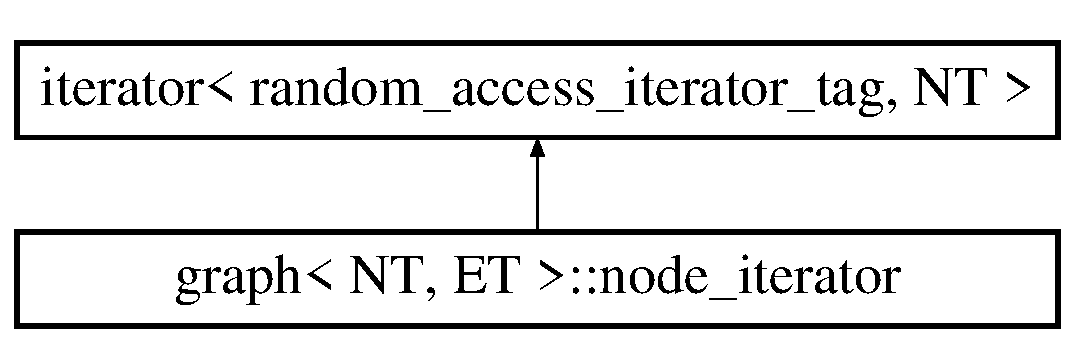
\includegraphics[height=2.000000cm]{classgraph_1_1node__iterator}
\end{center}
\end{figure}
\subsection*{Public Member Functions}
\begin{DoxyCompactItemize}
\item 
\hypertarget{classgraph_1_1node__iterator_af4cd87022aa1ab0b8f4d0a7088674142}{{\bfseries node\+\_\+iterator} (int index, const \hyperlink{classgraph}{graph} $\ast$g)}\label{classgraph_1_1node__iterator_af4cd87022aa1ab0b8f4d0a7088674142}

\item 
\hypertarget{classgraph_1_1node__iterator_ad72b585eff3afeefd58d33737a908f84}{const N\+T $\ast$ {\bfseries operator-\/$>$} () const }\label{classgraph_1_1node__iterator_ad72b585eff3afeefd58d33737a908f84}

\item 
\hypertarget{classgraph_1_1node__iterator_a879ba1aaf5dec3da103fdef088f479cd}{const N\+T \& {\bfseries operator$\ast$} () const }\label{classgraph_1_1node__iterator_a879ba1aaf5dec3da103fdef088f479cd}

\item 
\hypertarget{classgraph_1_1node__iterator_a5384f6440d2b625ec5cfa6f86cd2759b}{const \hyperlink{classgraph_1_1node__iterator}{node\+\_\+iterator} \& {\bfseries operator++} ()}\label{classgraph_1_1node__iterator_a5384f6440d2b625ec5cfa6f86cd2759b}

\item 
\hypertarget{classgraph_1_1node__iterator_ade76df2897a43b38180918e1876f36fe}{\hyperlink{classgraph_1_1node__iterator}{node\+\_\+iterator} {\bfseries operator++} (int)}\label{classgraph_1_1node__iterator_ade76df2897a43b38180918e1876f36fe}

\item 
\hypertarget{classgraph_1_1node__iterator_a27d188431fc8b976d1d4658b02a24726}{const \hyperlink{classgraph_1_1node__iterator}{node\+\_\+iterator} \& {\bfseries operator-\/-\/} ()}\label{classgraph_1_1node__iterator_a27d188431fc8b976d1d4658b02a24726}

\item 
\hypertarget{classgraph_1_1node__iterator_ad227228af099908edea6f38e02c72303}{\hyperlink{classgraph_1_1node__iterator}{node\+\_\+iterator} {\bfseries operator-\/-\/} (int)}\label{classgraph_1_1node__iterator_ad227228af099908edea6f38e02c72303}

\item 
\hypertarget{classgraph_1_1node__iterator_af2701cb2f00044bd1e2c850d65d32f5e}{const \hyperlink{classgraph_1_1node__iterator}{node\+\_\+iterator} \& {\bfseries operator+=} (int v)}\label{classgraph_1_1node__iterator_af2701cb2f00044bd1e2c850d65d32f5e}

\item 
\hypertarget{classgraph_1_1node__iterator_af155e6e177ee131be5af6fed46133f03}{const \hyperlink{classgraph_1_1node__iterator}{node\+\_\+iterator} \& {\bfseries operator-\/=} (int v)}\label{classgraph_1_1node__iterator_af155e6e177ee131be5af6fed46133f03}

\item 
\hypertarget{classgraph_1_1node__iterator_ad725e0ed27e4bd369a42d5db8eabcc47}{const N\+T \& {\bfseries operator\mbox{[}$\,$\mbox{]}} (int index2) const }\label{classgraph_1_1node__iterator_ad725e0ed27e4bd369a42d5db8eabcc47}

\item 
\hypertarget{classgraph_1_1node__iterator_a51e4cfdb48a739751fbde6b9352703d2}{const int {\bfseries position} () const }\label{classgraph_1_1node__iterator_a51e4cfdb48a739751fbde6b9352703d2}

\end{DoxyCompactItemize}
\subsection*{Private Member Functions}
\begin{DoxyCompactItemize}
\item 
\hypertarget{classgraph_1_1node__iterator_aac5a348f5d4079b0010238d91a9aaa12}{\hyperlink{structgraph_1_1Node}{Node} $\ast$ {\bfseries get} () const }\label{classgraph_1_1node__iterator_aac5a348f5d4079b0010238d91a9aaa12}

\end{DoxyCompactItemize}
\subsection*{Private Attributes}
\begin{DoxyCompactItemize}
\item 
\hypertarget{classgraph_1_1node__iterator_acb4fc8365499193998c097adea839971}{int {\bfseries index}}\label{classgraph_1_1node__iterator_acb4fc8365499193998c097adea839971}

\item 
\hypertarget{classgraph_1_1node__iterator_a52d58638288d1a746c262b0ae3409301}{const \hyperlink{classgraph}{graph} $\ast$ {\bfseries g}}\label{classgraph_1_1node__iterator_a52d58638288d1a746c262b0ae3409301}

\end{DoxyCompactItemize}
\subsection*{Friends}
\begin{DoxyCompactItemize}
\item 
\hypertarget{classgraph_1_1node__iterator_ab8b0dbc1b36724e5e4635ac651c218cb}{class {\bfseries graph}}\label{classgraph_1_1node__iterator_ab8b0dbc1b36724e5e4635ac651c218cb}

\item 
\hypertarget{classgraph_1_1node__iterator_a8a4971ebadf282168d84a07d4914c93c}{bool {\bfseries operator==} (const \hyperlink{classgraph_1_1node__iterator}{node\+\_\+iterator} \&l, const \hyperlink{classgraph_1_1node__iterator}{node\+\_\+iterator} \&r)}\label{classgraph_1_1node__iterator_a8a4971ebadf282168d84a07d4914c93c}

\item 
\hypertarget{classgraph_1_1node__iterator_ad75d23092c9ff953c3738f3454ccd9fb}{bool {\bfseries operator!=} (const \hyperlink{classgraph_1_1node__iterator}{node\+\_\+iterator} \&l, const \hyperlink{classgraph_1_1node__iterator}{node\+\_\+iterator} \&r)}\label{classgraph_1_1node__iterator_ad75d23092c9ff953c3738f3454ccd9fb}

\item 
\hypertarget{classgraph_1_1node__iterator_a6b1761a28d4367ba919c85f9f2c8d0e4}{\hyperlink{classgraph_1_1node__iterator}{node\+\_\+iterator} {\bfseries operator+} (int v, const \hyperlink{classgraph_1_1node__iterator}{node\+\_\+iterator} \&iter)}\label{classgraph_1_1node__iterator_a6b1761a28d4367ba919c85f9f2c8d0e4}

\item 
\hypertarget{classgraph_1_1node__iterator_a08e8068052fc1729d5b6a350e9dd1346}{\hyperlink{classgraph_1_1node__iterator}{node\+\_\+iterator} {\bfseries operator+} (const \hyperlink{classgraph_1_1node__iterator}{node\+\_\+iterator} \&iter, int v)}\label{classgraph_1_1node__iterator_a08e8068052fc1729d5b6a350e9dd1346}

\item 
\hypertarget{classgraph_1_1node__iterator_a0ac6efe2377fcbb51fe24924ce89608d}{\hyperlink{classgraph_1_1node__iterator}{node\+\_\+iterator} {\bfseries operator-\/} (const \hyperlink{classgraph_1_1node__iterator}{node\+\_\+iterator} \&iter, int v)}\label{classgraph_1_1node__iterator_a0ac6efe2377fcbb51fe24924ce89608d}

\item 
\hypertarget{classgraph_1_1node__iterator_aca04993c54f56e95d1be14feaeb7766f}{int {\bfseries operator-\/} (const \hyperlink{classgraph_1_1node__iterator}{node\+\_\+iterator} \&l, const \hyperlink{classgraph_1_1node__iterator}{node\+\_\+iterator} \&r)}\label{classgraph_1_1node__iterator_aca04993c54f56e95d1be14feaeb7766f}

\item 
\hypertarget{classgraph_1_1node__iterator_a545664b456b4e3c268ad91fec9e530b5}{bool {\bfseries operator$<$} (const \hyperlink{classgraph_1_1node__iterator}{node\+\_\+iterator} \&l, const \hyperlink{classgraph_1_1node__iterator}{node\+\_\+iterator} \&r)}\label{classgraph_1_1node__iterator_a545664b456b4e3c268ad91fec9e530b5}

\item 
\hypertarget{classgraph_1_1node__iterator_a538fbcfacacb3cf1ac7d3041b3342dc3}{bool {\bfseries operator$<$=} (const \hyperlink{classgraph_1_1node__iterator}{node\+\_\+iterator} \&l, const \hyperlink{classgraph_1_1node__iterator}{node\+\_\+iterator} \&r)}\label{classgraph_1_1node__iterator_a538fbcfacacb3cf1ac7d3041b3342dc3}

\item 
\hypertarget{classgraph_1_1node__iterator_a5d35f6f6fdf2dfeb5a7cdac7649b216f}{bool {\bfseries operator$>$=} (const \hyperlink{classgraph_1_1node__iterator}{node\+\_\+iterator} \&l, const \hyperlink{classgraph_1_1node__iterator}{node\+\_\+iterator} \&r)}\label{classgraph_1_1node__iterator_a5d35f6f6fdf2dfeb5a7cdac7649b216f}

\item 
\hypertarget{classgraph_1_1node__iterator_a74e84d83365092b345464ea91fc1b46c}{bool {\bfseries operator$>$} (const \hyperlink{classgraph_1_1node__iterator}{node\+\_\+iterator} \&l, const \hyperlink{classgraph_1_1node__iterator}{node\+\_\+iterator} \&r)}\label{classgraph_1_1node__iterator_a74e84d83365092b345464ea91fc1b46c}

\end{DoxyCompactItemize}


\subsection{Detailed Description}
\subsubsection*{template$<$typename N\+T, typename E\+T = N\+T$>$class graph$<$ N\+T, E\+T $>$\+::node\+\_\+iterator}



Definition at line 277 of file graph.\+h.



The documentation for this class was generated from the following file\+:\begin{DoxyCompactItemize}
\item 
graph.\+h\end{DoxyCompactItemize}

\hypertarget{classNodeEntryCollision}{\section{Node\+Entry\+Collision Class Reference}
\label{classNodeEntryCollision}\index{Node\+Entry\+Collision@{Node\+Entry\+Collision}}
}


\subsection{Detailed Description}


Definition at line 64 of file node.\+h.



The documentation for this class was generated from the following file\+:\begin{DoxyCompactItemize}
\item 
headers/node.\+h\end{DoxyCompactItemize}

\hypertarget{classNoStreamsLeftException}{\section{No\+Streams\+Left\+Exception Class Reference}
\label{classNoStreamsLeftException}\index{No\+Streams\+Left\+Exception@{No\+Streams\+Left\+Exception}}
}


Write what the function does here.  




{\ttfamily \#include $<$stream.\+h$>$}

Inheritance diagram for No\+Streams\+Left\+Exception\+:\begin{figure}[H]
\begin{center}
\leavevmode
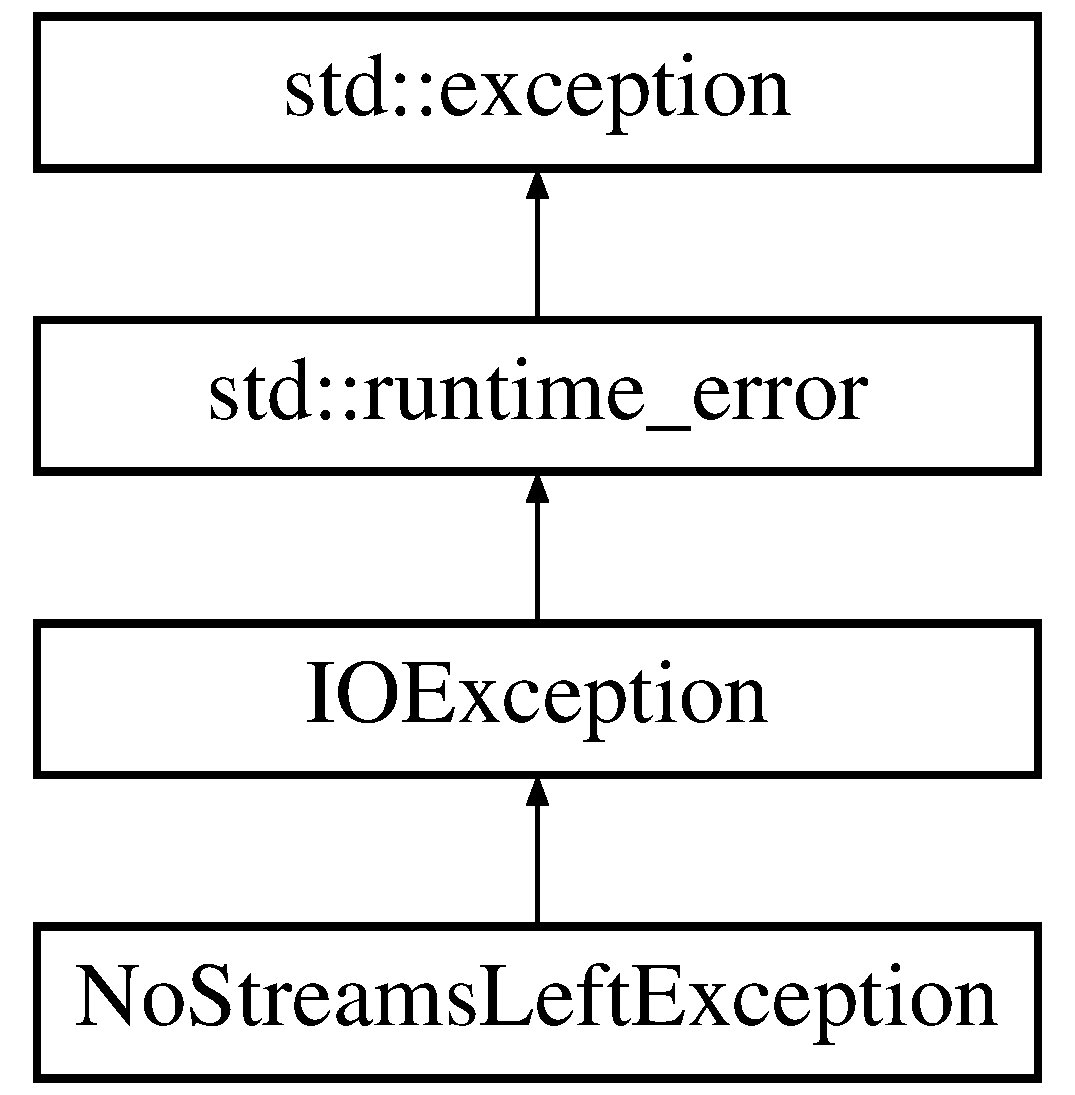
\includegraphics[height=4.000000cm]{classNoStreamsLeftException}
\end{center}
\end{figure}
\subsection*{Public Member Functions}
\begin{DoxyCompactItemize}
\item 
\hyperlink{classNoStreamsLeftException_a44c857faac6b8f16fa7dc2f701baf99b}{No\+Streams\+Left\+Exception} ()
\begin{DoxyCompactList}\small\item\em Write what the function does here. \end{DoxyCompactList}\end{DoxyCompactItemize}


\subsection{Detailed Description}
Write what the function does here. 

\begin{DoxyReturn}{Returns}

\end{DoxyReturn}


Definition at line 102 of file stream.\+h.



\subsection{Constructor \& Destructor Documentation}
\hypertarget{classNoStreamsLeftException_a44c857faac6b8f16fa7dc2f701baf99b}{\index{No\+Streams\+Left\+Exception@{No\+Streams\+Left\+Exception}!No\+Streams\+Left\+Exception@{No\+Streams\+Left\+Exception}}
\index{No\+Streams\+Left\+Exception@{No\+Streams\+Left\+Exception}!No\+Streams\+Left\+Exception@{No\+Streams\+Left\+Exception}}
\subsubsection[{No\+Streams\+Left\+Exception}]{\setlength{\rightskip}{0pt plus 5cm}No\+Streams\+Left\+Exception\+::\+No\+Streams\+Left\+Exception (
\begin{DoxyParamCaption}
{}
\end{DoxyParamCaption}
)\hspace{0.3cm}{\ttfamily [inline]}, {\ttfamily [explicit]}}}\label{classNoStreamsLeftException_a44c857faac6b8f16fa7dc2f701baf99b}


Write what the function does here. 

\begin{DoxyReturn}{Returns}

\end{DoxyReturn}


Definition at line 105 of file stream.\+h.


\begin{DoxyCode}
112             : \hyperlink{classIOException_a73fcf78b1b5820aa158680e896f0b983}{IOException}(\textcolor{stringliteral}{"IO Error : no streams left"})
113             \{
114             \}
\end{DoxyCode}


The documentation for this class was generated from the following file\+:\begin{DoxyCompactItemize}
\item 
stream.\+h\end{DoxyCompactItemize}

\hypertarget{classNotConnectable}{\section{Not\+Connectable Class Reference}
\label{classNotConnectable}\index{Not\+Connectable@{Not\+Connectable}}
}


\subsection{Detailed Description}


Definition at line 51 of file game.\+h.



The documentation for this class was generated from the following file\+:\begin{DoxyCompactItemize}
\item 
headers/game.\+h\end{DoxyCompactItemize}

\hypertarget{structpng__color__16__struct}{\section{png\+\_\+color\+\_\+16\+\_\+struct Struct Reference}
\label{structpng__color__16__struct}\index{png\+\_\+color\+\_\+16\+\_\+struct@{png\+\_\+color\+\_\+16\+\_\+struct}}
}
\subsection*{Public Attributes}
\begin{DoxyCompactItemize}
\item 
\hypertarget{structpng__color__16__struct_a44a918da0d9a50cf94fcad5a3c741ee0}{png\+\_\+byte {\bfseries index}}\label{structpng__color__16__struct_a44a918da0d9a50cf94fcad5a3c741ee0}

\item 
\hypertarget{structpng__color__16__struct_a069bad345aefbe4eab29fcc1d8af91e6}{png\+\_\+uint\+\_\+16 {\bfseries red}}\label{structpng__color__16__struct_a069bad345aefbe4eab29fcc1d8af91e6}

\item 
\hypertarget{structpng__color__16__struct_af01259ffd46c78eff9b1ad584a295126}{png\+\_\+uint\+\_\+16 {\bfseries green}}\label{structpng__color__16__struct_af01259ffd46c78eff9b1ad584a295126}

\item 
\hypertarget{structpng__color__16__struct_afd68833319d436582aa5911de7cdd46b}{png\+\_\+uint\+\_\+16 {\bfseries blue}}\label{structpng__color__16__struct_afd68833319d436582aa5911de7cdd46b}

\item 
\hypertarget{structpng__color__16__struct_a660a572a0a2f4094408f2fecb61571ac}{png\+\_\+uint\+\_\+16 {\bfseries gray}}\label{structpng__color__16__struct_a660a572a0a2f4094408f2fecb61571ac}

\end{DoxyCompactItemize}


\subsection{Detailed Description}


Definition at line 596 of file png.\+h.



The documentation for this struct was generated from the following file\+:\begin{DoxyCompactItemize}
\item 
png.\+h\end{DoxyCompactItemize}

\hypertarget{structpng__color__8__struct}{\section{png\+\_\+color\+\_\+8\+\_\+struct Struct Reference}
\label{structpng__color__8__struct}\index{png\+\_\+color\+\_\+8\+\_\+struct@{png\+\_\+color\+\_\+8\+\_\+struct}}
}
\subsection*{Public Attributes}
\begin{DoxyCompactItemize}
\item 
\hypertarget{structpng__color__8__struct_a5cd91bb4b3429256b84e6f28c72778b8}{png\+\_\+byte {\bfseries red}}\label{structpng__color__8__struct_a5cd91bb4b3429256b84e6f28c72778b8}

\item 
\hypertarget{structpng__color__8__struct_a40d053224177df35c037525b39563b05}{png\+\_\+byte {\bfseries green}}\label{structpng__color__8__struct_a40d053224177df35c037525b39563b05}

\item 
\hypertarget{structpng__color__8__struct_a58225d3b6426185d5a40d3c9935db96a}{png\+\_\+byte {\bfseries blue}}\label{structpng__color__8__struct_a58225d3b6426185d5a40d3c9935db96a}

\item 
\hypertarget{structpng__color__8__struct_a574edc173d956cca144927262e88653e}{png\+\_\+byte {\bfseries gray}}\label{structpng__color__8__struct_a574edc173d956cca144927262e88653e}

\item 
\hypertarget{structpng__color__8__struct_af1c7203aefe12bd35dc9a4cdd58e7a4b}{png\+\_\+byte {\bfseries alpha}}\label{structpng__color__8__struct_af1c7203aefe12bd35dc9a4cdd58e7a4b}

\end{DoxyCompactItemize}


\subsection{Detailed Description}


Definition at line 607 of file png.\+h.



The documentation for this struct was generated from the following file\+:\begin{DoxyCompactItemize}
\item 
png.\+h\end{DoxyCompactItemize}

\hypertarget{structpng__color__struct}{\section{png\+\_\+color\+\_\+struct Struct Reference}
\label{structpng__color__struct}\index{png\+\_\+color\+\_\+struct@{png\+\_\+color\+\_\+struct}}
}
\subsection*{Public Attributes}
\begin{DoxyCompactItemize}
\item 
\hypertarget{structpng__color__struct_ad39dc2d7cb82e3670a3ad397bb4083cb}{png\+\_\+byte {\bfseries red}}\label{structpng__color__struct_ad39dc2d7cb82e3670a3ad397bb4083cb}

\item 
\hypertarget{structpng__color__struct_ada9b5a911b185eaf7c6b87934e9f11ce}{png\+\_\+byte {\bfseries green}}\label{structpng__color__struct_ada9b5a911b185eaf7c6b87934e9f11ce}

\item 
\hypertarget{structpng__color__struct_a528e625b2778e787dc182e5df1164bbc}{png\+\_\+byte {\bfseries blue}}\label{structpng__color__struct_a528e625b2778e787dc182e5df1164bbc}

\end{DoxyCompactItemize}


\subsection{Detailed Description}


Definition at line 587 of file png.\+h.



The documentation for this struct was generated from the following file\+:\begin{DoxyCompactItemize}
\item 
png.\+h\end{DoxyCompactItemize}

\hypertarget{structpng__info__struct}{\section{png\+\_\+info\+\_\+struct Struct Reference}
\label{structpng__info__struct}\index{png\+\_\+info\+\_\+struct@{png\+\_\+info\+\_\+struct}}
}
\subsection*{Public Attributes}
\begin{DoxyCompactItemize}
\item 
\hypertarget{structpng__info__struct_aa47a2f299ef1098baf496eb2a13b4aea}{png\+\_\+uint\+\_\+32 {\bfseries width}}\label{structpng__info__struct_aa47a2f299ef1098baf496eb2a13b4aea}

\item 
\hypertarget{structpng__info__struct_a54ff13ac729e893eaedd5499a299ca2f}{png\+\_\+uint\+\_\+32 {\bfseries height}}\label{structpng__info__struct_a54ff13ac729e893eaedd5499a299ca2f}

\item 
\hypertarget{structpng__info__struct_a08aa92305b7d99d7106488382261a0e6}{png\+\_\+uint\+\_\+32 {\bfseries valid}}\label{structpng__info__struct_a08aa92305b7d99d7106488382261a0e6}

\item 
\hypertarget{structpng__info__struct_a8f5174bd85ca4fb3c861218308b251cf}{png\+\_\+uint\+\_\+32 {\bfseries rowbytes}}\label{structpng__info__struct_a8f5174bd85ca4fb3c861218308b251cf}

\item 
\hypertarget{structpng__info__struct_a964025dabd72160ffa2984040ddc5f3b}{png\+\_\+colorp {\bfseries palette}}\label{structpng__info__struct_a964025dabd72160ffa2984040ddc5f3b}

\item 
\hypertarget{structpng__info__struct_abf77cf402e77c9287dd0d366470c0d55}{png\+\_\+uint\+\_\+16 {\bfseries num\+\_\+palette}}\label{structpng__info__struct_abf77cf402e77c9287dd0d366470c0d55}

\item 
\hypertarget{structpng__info__struct_a47904541719f53ddccd79e09f87f3abb}{png\+\_\+uint\+\_\+16 {\bfseries num\+\_\+trans}}\label{structpng__info__struct_a47904541719f53ddccd79e09f87f3abb}

\item 
\hypertarget{structpng__info__struct_a492691764472633c7e046d0b80f9a3a5}{png\+\_\+byte {\bfseries bit\+\_\+depth}}\label{structpng__info__struct_a492691764472633c7e046d0b80f9a3a5}

\item 
\hypertarget{structpng__info__struct_ad8471eda4eb712d1f6f232db3fe7adb0}{png\+\_\+byte {\bfseries color\+\_\+type}}\label{structpng__info__struct_ad8471eda4eb712d1f6f232db3fe7adb0}

\item 
\hypertarget{structpng__info__struct_ab1889d1225872d5d406d2eda479bfc36}{png\+\_\+byte {\bfseries compression\+\_\+type}}\label{structpng__info__struct_ab1889d1225872d5d406d2eda479bfc36}

\item 
\hypertarget{structpng__info__struct_a6ae2423273fd0c4feae6e8ad34a3c3cd}{png\+\_\+byte {\bfseries filter\+\_\+type}}\label{structpng__info__struct_a6ae2423273fd0c4feae6e8ad34a3c3cd}

\item 
\hypertarget{structpng__info__struct_a8fce3b62a0744be86aacd2a3827bbaf6}{png\+\_\+byte {\bfseries interlace\+\_\+type}}\label{structpng__info__struct_a8fce3b62a0744be86aacd2a3827bbaf6}

\item 
\hypertarget{structpng__info__struct_a3e3f90075d35c903f290e1ec55d30ac6}{png\+\_\+byte {\bfseries channels}}\label{structpng__info__struct_a3e3f90075d35c903f290e1ec55d30ac6}

\item 
\hypertarget{structpng__info__struct_a487eecdd2dbc26656460012bdf85ff5a}{png\+\_\+byte {\bfseries pixel\+\_\+depth}}\label{structpng__info__struct_a487eecdd2dbc26656460012bdf85ff5a}

\item 
\hypertarget{structpng__info__struct_a44e2ae34ac6cb3e2809291ffbead76b3}{png\+\_\+byte {\bfseries spare\+\_\+byte}}\label{structpng__info__struct_a44e2ae34ac6cb3e2809291ffbead76b3}

\item 
\hypertarget{structpng__info__struct_ac72651ef050387991bb0c9b27d227a87}{png\+\_\+byte {\bfseries signature} \mbox{[}8\mbox{]}}\label{structpng__info__struct_ac72651ef050387991bb0c9b27d227a87}

\item 
\hypertarget{structpng__info__struct_a94f4f0d5679f86e35600e9b08362f9ff}{float {\bfseries gamma}}\label{structpng__info__struct_a94f4f0d5679f86e35600e9b08362f9ff}

\item 
\hypertarget{structpng__info__struct_ab436b3296441cd09ea0ba9471e798838}{png\+\_\+byte {\bfseries srgb\+\_\+intent}}\label{structpng__info__struct_ab436b3296441cd09ea0ba9471e798838}

\item 
\hypertarget{structpng__info__struct_a68485ae1bfea3f7b26e4ad0caaa02ad6}{int {\bfseries num\+\_\+text}}\label{structpng__info__struct_a68485ae1bfea3f7b26e4ad0caaa02ad6}

\item 
\hypertarget{structpng__info__struct_a2189e738364289ed6ad869a41f6f6384}{int {\bfseries max\+\_\+text}}\label{structpng__info__struct_a2189e738364289ed6ad869a41f6f6384}

\item 
\hypertarget{structpng__info__struct_a2c6bf85f9fe3331de438ac534f82c8c7}{png\+\_\+textp {\bfseries text}}\label{structpng__info__struct_a2c6bf85f9fe3331de438ac534f82c8c7}

\item 
\hypertarget{structpng__info__struct_a150966243a47afe8e64fa8c0f307bfb1}{\hyperlink{structpng__time__struct}{png\+\_\+time} {\bfseries mod\+\_\+time}}\label{structpng__info__struct_a150966243a47afe8e64fa8c0f307bfb1}

\item 
\hypertarget{structpng__info__struct_a0240a167cb880b831a8683223c1fb7cf}{\hyperlink{structpng__color__8__struct}{png\+\_\+color\+\_\+8} {\bfseries sig\+\_\+bit}}\label{structpng__info__struct_a0240a167cb880b831a8683223c1fb7cf}

\item 
\hypertarget{structpng__info__struct_add04ee373e415eccdf1d682e69a68dcd}{png\+\_\+bytep {\bfseries trans}}\label{structpng__info__struct_add04ee373e415eccdf1d682e69a68dcd}

\item 
\hypertarget{structpng__info__struct_ae68fbb1424443e75e730020beb299305}{\hyperlink{structpng__color__16__struct}{png\+\_\+color\+\_\+16} {\bfseries trans\+\_\+values}}\label{structpng__info__struct_ae68fbb1424443e75e730020beb299305}

\item 
\hypertarget{structpng__info__struct_a66e29accd9f0e1faf0950e72d2121f33}{\hyperlink{structpng__color__16__struct}{png\+\_\+color\+\_\+16} {\bfseries background}}\label{structpng__info__struct_a66e29accd9f0e1faf0950e72d2121f33}

\item 
\hypertarget{structpng__info__struct_af981f4ff0d05ae652a790f2b932d9749}{png\+\_\+int\+\_\+32 {\bfseries x\+\_\+offset}}\label{structpng__info__struct_af981f4ff0d05ae652a790f2b932d9749}

\item 
\hypertarget{structpng__info__struct_a00de4dbe2989f3e81a367ec699cc3499}{png\+\_\+int\+\_\+32 {\bfseries y\+\_\+offset}}\label{structpng__info__struct_a00de4dbe2989f3e81a367ec699cc3499}

\item 
\hypertarget{structpng__info__struct_aebf8d19c74f534eb653df73304e9cfde}{png\+\_\+byte {\bfseries offset\+\_\+unit\+\_\+type}}\label{structpng__info__struct_aebf8d19c74f534eb653df73304e9cfde}

\item 
\hypertarget{structpng__info__struct_af32f310bc311b5b649e9f8f5a5f70c1c}{png\+\_\+uint\+\_\+32 {\bfseries x\+\_\+pixels\+\_\+per\+\_\+unit}}\label{structpng__info__struct_af32f310bc311b5b649e9f8f5a5f70c1c}

\item 
\hypertarget{structpng__info__struct_a111c670b431bff35ea9a47cacf190250}{png\+\_\+uint\+\_\+32 {\bfseries y\+\_\+pixels\+\_\+per\+\_\+unit}}\label{structpng__info__struct_a111c670b431bff35ea9a47cacf190250}

\item 
\hypertarget{structpng__info__struct_ae8a1614b56762df135a28ec283a991e5}{png\+\_\+byte {\bfseries phys\+\_\+unit\+\_\+type}}\label{structpng__info__struct_ae8a1614b56762df135a28ec283a991e5}

\item 
\hypertarget{structpng__info__struct_a709ce088b8b66e6c0dfe7eef4caac686}{png\+\_\+uint\+\_\+16p {\bfseries hist}}\label{structpng__info__struct_a709ce088b8b66e6c0dfe7eef4caac686}

\item 
\hypertarget{structpng__info__struct_a62a1a82bf148f792c27a0779cecede9a}{float {\bfseries x\+\_\+white}}\label{structpng__info__struct_a62a1a82bf148f792c27a0779cecede9a}

\item 
\hypertarget{structpng__info__struct_a6a79d17fa0b75737d29ac69fc84c5977}{float {\bfseries y\+\_\+white}}\label{structpng__info__struct_a6a79d17fa0b75737d29ac69fc84c5977}

\item 
\hypertarget{structpng__info__struct_a71f22da2f24fad06e4eb4e976dc01f97}{float {\bfseries x\+\_\+red}}\label{structpng__info__struct_a71f22da2f24fad06e4eb4e976dc01f97}

\item 
\hypertarget{structpng__info__struct_a788f869127c0fc7f60c0a2fc32f3f492}{float {\bfseries y\+\_\+red}}\label{structpng__info__struct_a788f869127c0fc7f60c0a2fc32f3f492}

\item 
\hypertarget{structpng__info__struct_ab01f0096ed6cb61767ea8c835b651cf9}{float {\bfseries x\+\_\+green}}\label{structpng__info__struct_ab01f0096ed6cb61767ea8c835b651cf9}

\item 
\hypertarget{structpng__info__struct_aa30a2963392f0fe6685047f5890d7964}{float {\bfseries y\+\_\+green}}\label{structpng__info__struct_aa30a2963392f0fe6685047f5890d7964}

\item 
\hypertarget{structpng__info__struct_aabcb7bcf45b1034930b4afe6f5c5e8d1}{float {\bfseries x\+\_\+blue}}\label{structpng__info__struct_aabcb7bcf45b1034930b4afe6f5c5e8d1}

\item 
\hypertarget{structpng__info__struct_a0bf83d8ab283f01c92e8402af6836190}{float {\bfseries y\+\_\+blue}}\label{structpng__info__struct_a0bf83d8ab283f01c92e8402af6836190}

\item 
\hypertarget{structpng__info__struct_a8543337f34aa4a2226b8097060846f6f}{png\+\_\+charp {\bfseries pcal\+\_\+purpose}}\label{structpng__info__struct_a8543337f34aa4a2226b8097060846f6f}

\item 
\hypertarget{structpng__info__struct_a870761f88d3c0aa9d7bc5b91190e5e9f}{png\+\_\+int\+\_\+32 {\bfseries pcal\+\_\+\+X0}}\label{structpng__info__struct_a870761f88d3c0aa9d7bc5b91190e5e9f}

\item 
\hypertarget{structpng__info__struct_ac7466eb37166aa26cc0c378de765c7ff}{png\+\_\+int\+\_\+32 {\bfseries pcal\+\_\+\+X1}}\label{structpng__info__struct_ac7466eb37166aa26cc0c378de765c7ff}

\item 
\hypertarget{structpng__info__struct_a7486bac3111bcf3f2704731a09e8d6f2}{png\+\_\+charp {\bfseries pcal\+\_\+units}}\label{structpng__info__struct_a7486bac3111bcf3f2704731a09e8d6f2}

\item 
\hypertarget{structpng__info__struct_ad445745a6efb7f19fc03b0a3cb6e08aa}{png\+\_\+charpp {\bfseries pcal\+\_\+params}}\label{structpng__info__struct_ad445745a6efb7f19fc03b0a3cb6e08aa}

\item 
\hypertarget{structpng__info__struct_ac3be5c0fbb7858af28c9319ddb014099}{png\+\_\+byte {\bfseries pcal\+\_\+type}}\label{structpng__info__struct_ac3be5c0fbb7858af28c9319ddb014099}

\item 
\hypertarget{structpng__info__struct_a0cf3904f39e0c0af1f7c3b5bc3bfc33c}{png\+\_\+byte {\bfseries pcal\+\_\+nparams}}\label{structpng__info__struct_a0cf3904f39e0c0af1f7c3b5bc3bfc33c}

\item 
\hypertarget{structpng__info__struct_ac8cd35d4981fab722fb789cfdd8d531e}{png\+\_\+uint\+\_\+32 {\bfseries free\+\_\+me}}\label{structpng__info__struct_ac8cd35d4981fab722fb789cfdd8d531e}

\item 
\hypertarget{structpng__info__struct_a216ae5fb1daff66f9d461d1b1dbb6254}{png\+\_\+unknown\+\_\+chunkp {\bfseries unknown\+\_\+chunks}}\label{structpng__info__struct_a216ae5fb1daff66f9d461d1b1dbb6254}

\item 
\hypertarget{structpng__info__struct_a611e68d5c8760d5dde85a44ec298d456}{png\+\_\+size\+\_\+t {\bfseries unknown\+\_\+chunks\+\_\+num}}\label{structpng__info__struct_a611e68d5c8760d5dde85a44ec298d456}

\item 
\hypertarget{structpng__info__struct_ab76fd30aae356df7f503ada284fbb74f}{png\+\_\+charp {\bfseries iccp\+\_\+name}}\label{structpng__info__struct_ab76fd30aae356df7f503ada284fbb74f}

\item 
\hypertarget{structpng__info__struct_a3fc961c3925051a702b9177227702e3b}{png\+\_\+charp {\bfseries iccp\+\_\+profile}}\label{structpng__info__struct_a3fc961c3925051a702b9177227702e3b}

\item 
\hypertarget{structpng__info__struct_a87ad6f4d5e29d5c264ca8381ff0161ae}{png\+\_\+uint\+\_\+32 {\bfseries iccp\+\_\+proflen}}\label{structpng__info__struct_a87ad6f4d5e29d5c264ca8381ff0161ae}

\item 
\hypertarget{structpng__info__struct_a834367da72c7dee66161ce4cdabe3d9a}{png\+\_\+byte {\bfseries iccp\+\_\+compression}}\label{structpng__info__struct_a834367da72c7dee66161ce4cdabe3d9a}

\item 
\hypertarget{structpng__info__struct_a9df3d46242c72bbea6d9ca81c7e183f5}{png\+\_\+s\+P\+L\+T\+\_\+tp {\bfseries splt\+\_\+palettes}}\label{structpng__info__struct_a9df3d46242c72bbea6d9ca81c7e183f5}

\item 
\hypertarget{structpng__info__struct_a54b9d91e879bab87f3b9219a9528fcf1}{png\+\_\+uint\+\_\+32 {\bfseries splt\+\_\+palettes\+\_\+num}}\label{structpng__info__struct_a54b9d91e879bab87f3b9219a9528fcf1}

\item 
\hypertarget{structpng__info__struct_a05d48b7629ee75b0d6df1311cb11e82e}{png\+\_\+byte {\bfseries scal\+\_\+unit}}\label{structpng__info__struct_a05d48b7629ee75b0d6df1311cb11e82e}

\item 
\hypertarget{structpng__info__struct_a9241e751b9aca559f1c83d3a0640ef9e}{double {\bfseries scal\+\_\+pixel\+\_\+width}}\label{structpng__info__struct_a9241e751b9aca559f1c83d3a0640ef9e}

\item 
\hypertarget{structpng__info__struct_a7ee89c5ae94b74467e8fc7d550139e79}{double {\bfseries scal\+\_\+pixel\+\_\+height}}\label{structpng__info__struct_a7ee89c5ae94b74467e8fc7d550139e79}

\item 
\hypertarget{structpng__info__struct_a3505642667f6a587cf7789925753dfc9}{png\+\_\+charp {\bfseries scal\+\_\+s\+\_\+width}}\label{structpng__info__struct_a3505642667f6a587cf7789925753dfc9}

\item 
\hypertarget{structpng__info__struct_a19378bc934ab32d0ac299abb2fd09741}{png\+\_\+charp {\bfseries scal\+\_\+s\+\_\+height}}\label{structpng__info__struct_a19378bc934ab32d0ac299abb2fd09741}

\item 
\hypertarget{structpng__info__struct_a2e55fedc0e5c00021134ed1bd3adf77e}{png\+\_\+bytepp {\bfseries row\+\_\+pointers}}\label{structpng__info__struct_a2e55fedc0e5c00021134ed1bd3adf77e}

\item 
\hypertarget{structpng__info__struct_a3e3ad931ede73bdff68d19a5a14e97d6}{png\+\_\+fixed\+\_\+point {\bfseries int\+\_\+gamma}}\label{structpng__info__struct_a3e3ad931ede73bdff68d19a5a14e97d6}

\item 
\hypertarget{structpng__info__struct_a63e0819975b1a3dff01f23c67c86dd45}{png\+\_\+fixed\+\_\+point {\bfseries int\+\_\+x\+\_\+white}}\label{structpng__info__struct_a63e0819975b1a3dff01f23c67c86dd45}

\item 
\hypertarget{structpng__info__struct_a723808b3283cc5898546c1424bd5ed82}{png\+\_\+fixed\+\_\+point {\bfseries int\+\_\+y\+\_\+white}}\label{structpng__info__struct_a723808b3283cc5898546c1424bd5ed82}

\item 
\hypertarget{structpng__info__struct_a09eedbf9237962d4d45e71e7a2794fa5}{png\+\_\+fixed\+\_\+point {\bfseries int\+\_\+x\+\_\+red}}\label{structpng__info__struct_a09eedbf9237962d4d45e71e7a2794fa5}

\item 
\hypertarget{structpng__info__struct_a4e031ff94f4501210755a073e061bfa4}{png\+\_\+fixed\+\_\+point {\bfseries int\+\_\+y\+\_\+red}}\label{structpng__info__struct_a4e031ff94f4501210755a073e061bfa4}

\item 
\hypertarget{structpng__info__struct_a85faa4b47eed4fb1195956f915a5a211}{png\+\_\+fixed\+\_\+point {\bfseries int\+\_\+x\+\_\+green}}\label{structpng__info__struct_a85faa4b47eed4fb1195956f915a5a211}

\item 
\hypertarget{structpng__info__struct_ac196558e0bdf7a55aec72e2730d6f042}{png\+\_\+fixed\+\_\+point {\bfseries int\+\_\+y\+\_\+green}}\label{structpng__info__struct_ac196558e0bdf7a55aec72e2730d6f042}

\item 
\hypertarget{structpng__info__struct_a4844eadf8657ef08b6e7d577a0491538}{png\+\_\+fixed\+\_\+point {\bfseries int\+\_\+x\+\_\+blue}}\label{structpng__info__struct_a4844eadf8657ef08b6e7d577a0491538}

\item 
\hypertarget{structpng__info__struct_aba0a216dd3141d61b24b3a92a875a334}{png\+\_\+fixed\+\_\+point {\bfseries int\+\_\+y\+\_\+blue}}\label{structpng__info__struct_aba0a216dd3141d61b24b3a92a875a334}

\end{DoxyCompactItemize}


\subsection{Detailed Description}


Definition at line 768 of file png.\+h.



The documentation for this struct was generated from the following file\+:\begin{DoxyCompactItemize}
\item 
png.\+h\end{DoxyCompactItemize}

\hypertarget{structpng__row__info__struct}{\section{png\+\_\+row\+\_\+info\+\_\+struct Struct Reference}
\label{structpng__row__info__struct}\index{png\+\_\+row\+\_\+info\+\_\+struct@{png\+\_\+row\+\_\+info\+\_\+struct}}
}
\subsection*{Public Attributes}
\begin{DoxyCompactItemize}
\item 
\hypertarget{structpng__row__info__struct_a1ab107da5ffee8100eeaa76cc5ba3e62}{png\+\_\+uint\+\_\+32 {\bfseries width}}\label{structpng__row__info__struct_a1ab107da5ffee8100eeaa76cc5ba3e62}

\item 
\hypertarget{structpng__row__info__struct_a9a8c82137959d6d390ab2ccff87ea83b}{png\+\_\+uint\+\_\+32 {\bfseries rowbytes}}\label{structpng__row__info__struct_a9a8c82137959d6d390ab2ccff87ea83b}

\item 
\hypertarget{structpng__row__info__struct_a646244422549c66e6661cfcdb67c8e28}{png\+\_\+byte {\bfseries color\+\_\+type}}\label{structpng__row__info__struct_a646244422549c66e6661cfcdb67c8e28}

\item 
\hypertarget{structpng__row__info__struct_a6b14d5d0cc32f151c28c568cf1c1f82d}{png\+\_\+byte {\bfseries bit\+\_\+depth}}\label{structpng__row__info__struct_a6b14d5d0cc32f151c28c568cf1c1f82d}

\item 
\hypertarget{structpng__row__info__struct_a7cefee70361a3789a862001aefcd872f}{png\+\_\+byte {\bfseries channels}}\label{structpng__row__info__struct_a7cefee70361a3789a862001aefcd872f}

\item 
\hypertarget{structpng__row__info__struct_a70b84917ef9eabc9b7d29ec96fd01153}{png\+\_\+byte {\bfseries pixel\+\_\+depth}}\label{structpng__row__info__struct_a70b84917ef9eabc9b7d29ec96fd01153}

\end{DoxyCompactItemize}


\subsection{Detailed Description}


Definition at line 1110 of file png.\+h.



The documentation for this struct was generated from the following file\+:\begin{DoxyCompactItemize}
\item 
png.\+h\end{DoxyCompactItemize}

\hypertarget{structpng__sPLT__entry__struct}{\section{png\+\_\+s\+P\+L\+T\+\_\+entry\+\_\+struct Struct Reference}
\label{structpng__sPLT__entry__struct}\index{png\+\_\+s\+P\+L\+T\+\_\+entry\+\_\+struct@{png\+\_\+s\+P\+L\+T\+\_\+entry\+\_\+struct}}
}
\subsection*{Public Attributes}
\begin{DoxyCompactItemize}
\item 
\hypertarget{structpng__sPLT__entry__struct_a05ba3cef8aa2c43d1f52c0300c525fd9}{png\+\_\+uint\+\_\+16 {\bfseries red}}\label{structpng__sPLT__entry__struct_a05ba3cef8aa2c43d1f52c0300c525fd9}

\item 
\hypertarget{structpng__sPLT__entry__struct_a3b4269fb63b4087bd618a6741b805554}{png\+\_\+uint\+\_\+16 {\bfseries green}}\label{structpng__sPLT__entry__struct_a3b4269fb63b4087bd618a6741b805554}

\item 
\hypertarget{structpng__sPLT__entry__struct_a2af6281d3b400362886a43977ebcb7db}{png\+\_\+uint\+\_\+16 {\bfseries blue}}\label{structpng__sPLT__entry__struct_a2af6281d3b400362886a43977ebcb7db}

\item 
\hypertarget{structpng__sPLT__entry__struct_abea98962a064e2a05f460b9f2ea2f47b}{png\+\_\+uint\+\_\+16 {\bfseries alpha}}\label{structpng__sPLT__entry__struct_abea98962a064e2a05f460b9f2ea2f47b}

\item 
\hypertarget{structpng__sPLT__entry__struct_ad8095a15bb5a054c12ef911478c5f3a3}{png\+\_\+uint\+\_\+16 {\bfseries frequency}}\label{structpng__sPLT__entry__struct_ad8095a15bb5a054c12ef911478c5f3a3}

\end{DoxyCompactItemize}


\subsection{Detailed Description}


Definition at line 622 of file png.\+h.



The documentation for this struct was generated from the following file\+:\begin{DoxyCompactItemize}
\item 
png.\+h\end{DoxyCompactItemize}

\hypertarget{structpng__sPLT__struct}{\section{png\+\_\+s\+P\+L\+T\+\_\+struct Struct Reference}
\label{structpng__sPLT__struct}\index{png\+\_\+s\+P\+L\+T\+\_\+struct@{png\+\_\+s\+P\+L\+T\+\_\+struct}}
}
\subsection*{Public Attributes}
\begin{DoxyCompactItemize}
\item 
\hypertarget{structpng__sPLT__struct_af3b088b149e790b9b98ebedde69a70f0}{png\+\_\+charp {\bfseries name}}\label{structpng__sPLT__struct_af3b088b149e790b9b98ebedde69a70f0}

\item 
\hypertarget{structpng__sPLT__struct_a6e667882cd16c9675455cebd49898b22}{png\+\_\+byte {\bfseries depth}}\label{structpng__sPLT__struct_a6e667882cd16c9675455cebd49898b22}

\item 
\hypertarget{structpng__sPLT__struct_a4c7db13fb1a7f0ede434e174b20151ec}{png\+\_\+s\+P\+L\+T\+\_\+entryp {\bfseries entries}}\label{structpng__sPLT__struct_a4c7db13fb1a7f0ede434e174b20151ec}

\item 
\hypertarget{structpng__sPLT__struct_ac5844e98e4c43733bad6b83b54dc7a9f}{png\+\_\+int\+\_\+32 {\bfseries nentries}}\label{structpng__sPLT__struct_ac5844e98e4c43733bad6b83b54dc7a9f}

\end{DoxyCompactItemize}


\subsection{Detailed Description}


Definition at line 638 of file png.\+h.



The documentation for this struct was generated from the following file\+:\begin{DoxyCompactItemize}
\item 
png.\+h\end{DoxyCompactItemize}

\hypertarget{structpng__struct__def}{\section{png\+\_\+struct\+\_\+def Struct Reference}
\label{structpng__struct__def}\index{png\+\_\+struct\+\_\+def@{png\+\_\+struct\+\_\+def}}
}
\subsection*{Public Attributes}
\begin{DoxyCompactItemize}
\item 
\hypertarget{structpng__struct__def_a612a97110a82e8481d68bb7ef47f6224}{jmp\+\_\+buf {\bfseries jmpbuf}}\label{structpng__struct__def_a612a97110a82e8481d68bb7ef47f6224}

\item 
\hypertarget{structpng__struct__def_a2cc5bd1cf507373992a61cf725a730cd}{png\+\_\+error\+\_\+ptr {\bfseries error\+\_\+fn}}\label{structpng__struct__def_a2cc5bd1cf507373992a61cf725a730cd}

\item 
\hypertarget{structpng__struct__def_a43bba3b1d80a9a21ea9d4d55da13eafd}{png\+\_\+error\+\_\+ptr {\bfseries warning\+\_\+fn}}\label{structpng__struct__def_a43bba3b1d80a9a21ea9d4d55da13eafd}

\item 
\hypertarget{structpng__struct__def_a06837611b772a6a44cf6306ea08d40a8}{png\+\_\+voidp {\bfseries error\+\_\+ptr}}\label{structpng__struct__def_a06837611b772a6a44cf6306ea08d40a8}

\item 
\hypertarget{structpng__struct__def_acc53cd87f0ffc4d1f67da7e10a94af39}{png\+\_\+rw\+\_\+ptr {\bfseries write\+\_\+data\+\_\+fn}}\label{structpng__struct__def_acc53cd87f0ffc4d1f67da7e10a94af39}

\item 
\hypertarget{structpng__struct__def_a83804076437d1587fab947c056bb56ae}{png\+\_\+rw\+\_\+ptr {\bfseries read\+\_\+data\+\_\+fn}}\label{structpng__struct__def_a83804076437d1587fab947c056bb56ae}

\item 
\hypertarget{structpng__struct__def_a996f6f8aaa00ede3bb147714ee7c480e}{png\+\_\+voidp {\bfseries io\+\_\+ptr}}\label{structpng__struct__def_a996f6f8aaa00ede3bb147714ee7c480e}

\item 
\hypertarget{structpng__struct__def_a7fd40a67ea39220221977700bce18dac}{png\+\_\+user\+\_\+transform\+\_\+ptr {\bfseries read\+\_\+user\+\_\+transform\+\_\+fn}}\label{structpng__struct__def_a7fd40a67ea39220221977700bce18dac}

\item 
\hypertarget{structpng__struct__def_afec7d5da6863af6d349a67674fd8a940}{png\+\_\+user\+\_\+transform\+\_\+ptr {\bfseries write\+\_\+user\+\_\+transform\+\_\+fn}}\label{structpng__struct__def_afec7d5da6863af6d349a67674fd8a940}

\item 
\hypertarget{structpng__struct__def_aa867d0801e45c3bf636be098958ebcd8}{png\+\_\+voidp {\bfseries user\+\_\+transform\+\_\+ptr}}\label{structpng__struct__def_aa867d0801e45c3bf636be098958ebcd8}

\item 
\hypertarget{structpng__struct__def_ad4fe873c4d7be923efb5bde5db223274}{png\+\_\+byte {\bfseries user\+\_\+transform\+\_\+depth}}\label{structpng__struct__def_ad4fe873c4d7be923efb5bde5db223274}

\item 
\hypertarget{structpng__struct__def_ac9bc0f519d1f5c949e2e19dfc7457339}{png\+\_\+byte {\bfseries user\+\_\+transform\+\_\+channels}}\label{structpng__struct__def_ac9bc0f519d1f5c949e2e19dfc7457339}

\item 
\hypertarget{structpng__struct__def_a6db33193ca2fdb01fa6d8da9756bd448}{png\+\_\+uint\+\_\+32 {\bfseries mode}}\label{structpng__struct__def_a6db33193ca2fdb01fa6d8da9756bd448}

\item 
\hypertarget{structpng__struct__def_aa7529cc3d13e759037c504fddd6e1ae8}{png\+\_\+uint\+\_\+32 {\bfseries flags}}\label{structpng__struct__def_aa7529cc3d13e759037c504fddd6e1ae8}

\item 
\hypertarget{structpng__struct__def_a4ab3e33248dd4c32880609a1a10fa725}{png\+\_\+uint\+\_\+32 {\bfseries transformations}}\label{structpng__struct__def_a4ab3e33248dd4c32880609a1a10fa725}

\item 
\hypertarget{structpng__struct__def_aed56a6997ce7d1a90f0a143eb0964cd5}{\hyperlink{structz__stream__s}{z\+\_\+stream} {\bfseries zstream}}\label{structpng__struct__def_aed56a6997ce7d1a90f0a143eb0964cd5}

\item 
\hypertarget{structpng__struct__def_a8cd7436515e6ee37b4b895b4470ab052}{png\+\_\+bytep {\bfseries zbuf}}\label{structpng__struct__def_a8cd7436515e6ee37b4b895b4470ab052}

\item 
\hypertarget{structpng__struct__def_a7a4643dd3086efd14aa9708452c3fe2e}{png\+\_\+size\+\_\+t {\bfseries zbuf\+\_\+size}}\label{structpng__struct__def_a7a4643dd3086efd14aa9708452c3fe2e}

\item 
\hypertarget{structpng__struct__def_a3a92fe2ce08200b841be61c9d6f1d7c3}{int {\bfseries zlib\+\_\+level}}\label{structpng__struct__def_a3a92fe2ce08200b841be61c9d6f1d7c3}

\item 
\hypertarget{structpng__struct__def_ae2ee3f62068a9968fce33005c61fd1c9}{int {\bfseries zlib\+\_\+method}}\label{structpng__struct__def_ae2ee3f62068a9968fce33005c61fd1c9}

\item 
\hypertarget{structpng__struct__def_a61ecd429af47e450e5162bcd894d5622}{int {\bfseries zlib\+\_\+window\+\_\+bits}}\label{structpng__struct__def_a61ecd429af47e450e5162bcd894d5622}

\item 
\hypertarget{structpng__struct__def_af3e2255f307d2218192fae9edfb374b5}{int {\bfseries zlib\+\_\+mem\+\_\+level}}\label{structpng__struct__def_af3e2255f307d2218192fae9edfb374b5}

\item 
\hypertarget{structpng__struct__def_a19e170deba8613eefc74c6d8afafc229}{int {\bfseries zlib\+\_\+strategy}}\label{structpng__struct__def_a19e170deba8613eefc74c6d8afafc229}

\item 
\hypertarget{structpng__struct__def_abb11531c781ea91b63d0fa1af122eaab}{png\+\_\+uint\+\_\+32 {\bfseries width}}\label{structpng__struct__def_abb11531c781ea91b63d0fa1af122eaab}

\item 
\hypertarget{structpng__struct__def_a1dd47d897b96de5b8c12a242695adad5}{png\+\_\+uint\+\_\+32 {\bfseries height}}\label{structpng__struct__def_a1dd47d897b96de5b8c12a242695adad5}

\item 
\hypertarget{structpng__struct__def_a209926649ef1f0bb46ea0f277041ce78}{png\+\_\+uint\+\_\+32 {\bfseries num\+\_\+rows}}\label{structpng__struct__def_a209926649ef1f0bb46ea0f277041ce78}

\item 
\hypertarget{structpng__struct__def_a6fb8c450c20bc0161211b00a18db173e}{png\+\_\+uint\+\_\+32 {\bfseries usr\+\_\+width}}\label{structpng__struct__def_a6fb8c450c20bc0161211b00a18db173e}

\item 
\hypertarget{structpng__struct__def_ad05e410ff54555283b16670e35be4db2}{png\+\_\+uint\+\_\+32 {\bfseries rowbytes}}\label{structpng__struct__def_ad05e410ff54555283b16670e35be4db2}

\item 
\hypertarget{structpng__struct__def_aa922e94a9862d832ffe839210db5aaa2}{png\+\_\+uint\+\_\+32 {\bfseries irowbytes}}\label{structpng__struct__def_aa922e94a9862d832ffe839210db5aaa2}

\item 
\hypertarget{structpng__struct__def_a6323d3dc2ce858895c889716aba45b17}{png\+\_\+uint\+\_\+32 {\bfseries iwidth}}\label{structpng__struct__def_a6323d3dc2ce858895c889716aba45b17}

\item 
\hypertarget{structpng__struct__def_a0f06a454e8369cbbb90be4b5ab25654c}{png\+\_\+uint\+\_\+32 {\bfseries row\+\_\+number}}\label{structpng__struct__def_a0f06a454e8369cbbb90be4b5ab25654c}

\item 
\hypertarget{structpng__struct__def_af307f45d48c7900d1036388bccbed7bb}{png\+\_\+bytep {\bfseries prev\+\_\+row}}\label{structpng__struct__def_af307f45d48c7900d1036388bccbed7bb}

\item 
\hypertarget{structpng__struct__def_a05b648068595d5cf4400c0709cb0012d}{png\+\_\+bytep {\bfseries row\+\_\+buf}}\label{structpng__struct__def_a05b648068595d5cf4400c0709cb0012d}

\item 
\hypertarget{structpng__struct__def_a9cd0e758b239d083a65f639e400312b1}{png\+\_\+bytep {\bfseries sub\+\_\+row}}\label{structpng__struct__def_a9cd0e758b239d083a65f639e400312b1}

\item 
\hypertarget{structpng__struct__def_a84d3819171a64f58f01705d6e83e30f6}{png\+\_\+bytep {\bfseries up\+\_\+row}}\label{structpng__struct__def_a84d3819171a64f58f01705d6e83e30f6}

\item 
\hypertarget{structpng__struct__def_a8d0d3a1345f9a7f809e5090b3c127b12}{png\+\_\+bytep {\bfseries avg\+\_\+row}}\label{structpng__struct__def_a8d0d3a1345f9a7f809e5090b3c127b12}

\item 
\hypertarget{structpng__struct__def_aa139b001143e359e8f938f9f30f90e82}{png\+\_\+bytep {\bfseries paeth\+\_\+row}}\label{structpng__struct__def_aa139b001143e359e8f938f9f30f90e82}

\item 
\hypertarget{structpng__struct__def_ac9ac1f3db591736db145aea42dfb4bc5}{\hyperlink{structpng__row__info__struct}{png\+\_\+row\+\_\+info} {\bfseries row\+\_\+info}}\label{structpng__struct__def_ac9ac1f3db591736db145aea42dfb4bc5}

\item 
\hypertarget{structpng__struct__def_ab6951f7357162b382c2647a8d577d5b3}{png\+\_\+uint\+\_\+32 {\bfseries idat\+\_\+size}}\label{structpng__struct__def_ab6951f7357162b382c2647a8d577d5b3}

\item 
\hypertarget{structpng__struct__def_a41e688627efdb841bb3c7e49b6872f0c}{png\+\_\+uint\+\_\+32 {\bfseries crc}}\label{structpng__struct__def_a41e688627efdb841bb3c7e49b6872f0c}

\item 
\hypertarget{structpng__struct__def_ae79416e3df9e02b8a17eac57f91b6fc0}{png\+\_\+colorp {\bfseries palette}}\label{structpng__struct__def_ae79416e3df9e02b8a17eac57f91b6fc0}

\item 
\hypertarget{structpng__struct__def_a55dc88ce7229269ae06c498e63a00ccc}{png\+\_\+uint\+\_\+16 {\bfseries num\+\_\+palette}}\label{structpng__struct__def_a55dc88ce7229269ae06c498e63a00ccc}

\item 
\hypertarget{structpng__struct__def_a3988e717574b747396cb156e29895cb0}{png\+\_\+uint\+\_\+16 {\bfseries num\+\_\+trans}}\label{structpng__struct__def_a3988e717574b747396cb156e29895cb0}

\item 
\hypertarget{structpng__struct__def_a7ccc46aaf4795263454b14c9304f3301}{png\+\_\+byte {\bfseries chunk\+\_\+name} \mbox{[}5\mbox{]}}\label{structpng__struct__def_a7ccc46aaf4795263454b14c9304f3301}

\item 
\hypertarget{structpng__struct__def_a535707a3578321703642be999866f131}{png\+\_\+byte {\bfseries compression}}\label{structpng__struct__def_a535707a3578321703642be999866f131}

\item 
\hypertarget{structpng__struct__def_a4680ad260ea37a0b69677ff537b1c8b1}{png\+\_\+byte {\bfseries filter}}\label{structpng__struct__def_a4680ad260ea37a0b69677ff537b1c8b1}

\item 
\hypertarget{structpng__struct__def_ac57d1535c25726a4080f4f471dbb7e17}{png\+\_\+byte {\bfseries interlaced}}\label{structpng__struct__def_ac57d1535c25726a4080f4f471dbb7e17}

\item 
\hypertarget{structpng__struct__def_a61226f1790d295a85fdd0ca8c195469c}{png\+\_\+byte {\bfseries pass}}\label{structpng__struct__def_a61226f1790d295a85fdd0ca8c195469c}

\item 
\hypertarget{structpng__struct__def_abcbabd6f1568b3924af91556371d7b73}{png\+\_\+byte {\bfseries do\+\_\+filter}}\label{structpng__struct__def_abcbabd6f1568b3924af91556371d7b73}

\item 
\hypertarget{structpng__struct__def_a01e64966deb22a659cce371cbf6af666}{png\+\_\+byte {\bfseries color\+\_\+type}}\label{structpng__struct__def_a01e64966deb22a659cce371cbf6af666}

\item 
\hypertarget{structpng__struct__def_a8a18c35f00b4dff31c12306156f01ce3}{png\+\_\+byte {\bfseries bit\+\_\+depth}}\label{structpng__struct__def_a8a18c35f00b4dff31c12306156f01ce3}

\item 
\hypertarget{structpng__struct__def_af30e53e1cad0830302030152c81cc59f}{png\+\_\+byte {\bfseries usr\+\_\+bit\+\_\+depth}}\label{structpng__struct__def_af30e53e1cad0830302030152c81cc59f}

\item 
\hypertarget{structpng__struct__def_ac7a7265bc00d1fd48a8eb20727f53fa1}{png\+\_\+byte {\bfseries pixel\+\_\+depth}}\label{structpng__struct__def_ac7a7265bc00d1fd48a8eb20727f53fa1}

\item 
\hypertarget{structpng__struct__def_a6cc1ac2587b192b7220639ab719f2b73}{png\+\_\+byte {\bfseries channels}}\label{structpng__struct__def_a6cc1ac2587b192b7220639ab719f2b73}

\item 
\hypertarget{structpng__struct__def_ababe2bb7d779b4334a95b73c763b472c}{png\+\_\+byte {\bfseries usr\+\_\+channels}}\label{structpng__struct__def_ababe2bb7d779b4334a95b73c763b472c}

\item 
\hypertarget{structpng__struct__def_a019243f63de45bd677d23f8ed533679d}{png\+\_\+byte {\bfseries sig\+\_\+bytes}}\label{structpng__struct__def_a019243f63de45bd677d23f8ed533679d}

\item 
\hypertarget{structpng__struct__def_a89c290f398edd77800b7ca4b3331f727}{png\+\_\+uint\+\_\+16 {\bfseries filler}}\label{structpng__struct__def_a89c290f398edd77800b7ca4b3331f727}

\item 
\hypertarget{structpng__struct__def_a2ddb3bedc92ad2e8be70e3c7f3f38fa6}{png\+\_\+byte {\bfseries background\+\_\+gamma\+\_\+type}}\label{structpng__struct__def_a2ddb3bedc92ad2e8be70e3c7f3f38fa6}

\item 
\hypertarget{structpng__struct__def_a39e06c269454f5d93f55f2855da735af}{float {\bfseries background\+\_\+gamma}}\label{structpng__struct__def_a39e06c269454f5d93f55f2855da735af}

\item 
\hypertarget{structpng__struct__def_a5176d0fc24966a534e71b64a0f8eb763}{\hyperlink{structpng__color__16__struct}{png\+\_\+color\+\_\+16} {\bfseries background}}\label{structpng__struct__def_a5176d0fc24966a534e71b64a0f8eb763}

\item 
\hypertarget{structpng__struct__def_aaf3c55b65526060835b089f49b65189a}{\hyperlink{structpng__color__16__struct}{png\+\_\+color\+\_\+16} {\bfseries background\+\_\+1}}\label{structpng__struct__def_aaf3c55b65526060835b089f49b65189a}

\item 
\hypertarget{structpng__struct__def_a7b115e3413a6d7d414feab232220773d}{png\+\_\+flush\+\_\+ptr {\bfseries output\+\_\+flush\+\_\+fn}}\label{structpng__struct__def_a7b115e3413a6d7d414feab232220773d}

\item 
\hypertarget{structpng__struct__def_a8f50672475e3b0464738889ce7d65656}{png\+\_\+uint\+\_\+32 {\bfseries flush\+\_\+dist}}\label{structpng__struct__def_a8f50672475e3b0464738889ce7d65656}

\item 
\hypertarget{structpng__struct__def_a1657329d0573f2b7e93ee3e35c5751ca}{png\+\_\+uint\+\_\+32 {\bfseries flush\+\_\+rows}}\label{structpng__struct__def_a1657329d0573f2b7e93ee3e35c5751ca}

\item 
\hypertarget{structpng__struct__def_a3459e4958374e7e571bcadcc7a79eef4}{int {\bfseries gamma\+\_\+shift}}\label{structpng__struct__def_a3459e4958374e7e571bcadcc7a79eef4}

\item 
\hypertarget{structpng__struct__def_a6ab9fd579c9d9862c45433f2a94b5c47}{float {\bfseries gamma}}\label{structpng__struct__def_a6ab9fd579c9d9862c45433f2a94b5c47}

\item 
\hypertarget{structpng__struct__def_a9a984aa9faec4a492c0d8d5ce227a4e5}{float {\bfseries screen\+\_\+gamma}}\label{structpng__struct__def_a9a984aa9faec4a492c0d8d5ce227a4e5}

\item 
\hypertarget{structpng__struct__def_a4e97701069f1d5bb563f607591350200}{png\+\_\+bytep {\bfseries gamma\+\_\+table}}\label{structpng__struct__def_a4e97701069f1d5bb563f607591350200}

\item 
\hypertarget{structpng__struct__def_a22b2414d75791e0cdf225b08a2291066}{png\+\_\+bytep {\bfseries gamma\+\_\+from\+\_\+1}}\label{structpng__struct__def_a22b2414d75791e0cdf225b08a2291066}

\item 
\hypertarget{structpng__struct__def_a1fde49c336ba766ff4ceb837dcc1c1b9}{png\+\_\+bytep {\bfseries gamma\+\_\+to\+\_\+1}}\label{structpng__struct__def_a1fde49c336ba766ff4ceb837dcc1c1b9}

\item 
\hypertarget{structpng__struct__def_abeec3753c2603f799e6ba62c42e86b80}{png\+\_\+uint\+\_\+16pp {\bfseries gamma\+\_\+16\+\_\+table}}\label{structpng__struct__def_abeec3753c2603f799e6ba62c42e86b80}

\item 
\hypertarget{structpng__struct__def_a6acfc95f4c725c721063a47497f71b11}{png\+\_\+uint\+\_\+16pp {\bfseries gamma\+\_\+16\+\_\+from\+\_\+1}}\label{structpng__struct__def_a6acfc95f4c725c721063a47497f71b11}

\item 
\hypertarget{structpng__struct__def_a40f1b82331e8e2b2dce68ec94a8d7386}{png\+\_\+uint\+\_\+16pp {\bfseries gamma\+\_\+16\+\_\+to\+\_\+1}}\label{structpng__struct__def_a40f1b82331e8e2b2dce68ec94a8d7386}

\item 
\hypertarget{structpng__struct__def_addb89a2342bf0fb90396de1e12d8f917}{\hyperlink{structpng__color__8__struct}{png\+\_\+color\+\_\+8} {\bfseries sig\+\_\+bit}}\label{structpng__struct__def_addb89a2342bf0fb90396de1e12d8f917}

\item 
\hypertarget{structpng__struct__def_a8760d720ca9f015590a87d970cbe7b70}{\hyperlink{structpng__color__8__struct}{png\+\_\+color\+\_\+8} {\bfseries shift}}\label{structpng__struct__def_a8760d720ca9f015590a87d970cbe7b70}

\item 
\hypertarget{structpng__struct__def_af737bf346b298c74cd5ffaaab652983d}{png\+\_\+bytep {\bfseries trans}}\label{structpng__struct__def_af737bf346b298c74cd5ffaaab652983d}

\item 
\hypertarget{structpng__struct__def_aa3c2191d2c1525169a3c1687bcb40cc2}{\hyperlink{structpng__color__16__struct}{png\+\_\+color\+\_\+16} {\bfseries trans\+\_\+values}}\label{structpng__struct__def_aa3c2191d2c1525169a3c1687bcb40cc2}

\item 
\hypertarget{structpng__struct__def_a0d67c044d4088f4673b90c2109ff94c0}{png\+\_\+read\+\_\+status\+\_\+ptr {\bfseries read\+\_\+row\+\_\+fn}}\label{structpng__struct__def_a0d67c044d4088f4673b90c2109ff94c0}

\item 
\hypertarget{structpng__struct__def_a1ea44e185e0f8bdd7299f93fd017c32c}{png\+\_\+write\+\_\+status\+\_\+ptr {\bfseries write\+\_\+row\+\_\+fn}}\label{structpng__struct__def_a1ea44e185e0f8bdd7299f93fd017c32c}

\item 
\hypertarget{structpng__struct__def_aef67c330c01d2075e65546b9095d34db}{png\+\_\+progressive\+\_\+info\+\_\+ptr {\bfseries info\+\_\+fn}}\label{structpng__struct__def_aef67c330c01d2075e65546b9095d34db}

\item 
\hypertarget{structpng__struct__def_a6664476189226b96b0ef48ad30260fff}{png\+\_\+progressive\+\_\+row\+\_\+ptr {\bfseries row\+\_\+fn}}\label{structpng__struct__def_a6664476189226b96b0ef48ad30260fff}

\item 
\hypertarget{structpng__struct__def_aa4b1e2dbc6aee34901d428d819d2b0b7}{png\+\_\+progressive\+\_\+end\+\_\+ptr {\bfseries end\+\_\+fn}}\label{structpng__struct__def_aa4b1e2dbc6aee34901d428d819d2b0b7}

\item 
\hypertarget{structpng__struct__def_a10d994882cca7c4f6ae05d1a7267f6f8}{png\+\_\+bytep {\bfseries save\+\_\+buffer\+\_\+ptr}}\label{structpng__struct__def_a10d994882cca7c4f6ae05d1a7267f6f8}

\item 
\hypertarget{structpng__struct__def_aa1739642adc16dba8dc9c519aed51591}{png\+\_\+bytep {\bfseries save\+\_\+buffer}}\label{structpng__struct__def_aa1739642adc16dba8dc9c519aed51591}

\item 
\hypertarget{structpng__struct__def_a563e0a93065539cc4b236a8d8b78368d}{png\+\_\+bytep {\bfseries current\+\_\+buffer\+\_\+ptr}}\label{structpng__struct__def_a563e0a93065539cc4b236a8d8b78368d}

\item 
\hypertarget{structpng__struct__def_a1d1c579dc75685ba1998dfdd1698faad}{png\+\_\+bytep {\bfseries current\+\_\+buffer}}\label{structpng__struct__def_a1d1c579dc75685ba1998dfdd1698faad}

\item 
\hypertarget{structpng__struct__def_a62f744f346e1cd6f711bd58cbe95f283}{png\+\_\+uint\+\_\+32 {\bfseries push\+\_\+length}}\label{structpng__struct__def_a62f744f346e1cd6f711bd58cbe95f283}

\item 
\hypertarget{structpng__struct__def_a83f10d8423ee0fac3f0cf89669405e80}{png\+\_\+uint\+\_\+32 {\bfseries skip\+\_\+length}}\label{structpng__struct__def_a83f10d8423ee0fac3f0cf89669405e80}

\item 
\hypertarget{structpng__struct__def_a6c9dff0d2113501c73a57b83ff4dbd33}{png\+\_\+size\+\_\+t {\bfseries save\+\_\+buffer\+\_\+size}}\label{structpng__struct__def_a6c9dff0d2113501c73a57b83ff4dbd33}

\item 
\hypertarget{structpng__struct__def_a8bb4bcefb46c9bbacd78c0e9a1ced8c8}{png\+\_\+size\+\_\+t {\bfseries save\+\_\+buffer\+\_\+max}}\label{structpng__struct__def_a8bb4bcefb46c9bbacd78c0e9a1ced8c8}

\item 
\hypertarget{structpng__struct__def_a0b8efec98c80bf8163e3054eb8937984}{png\+\_\+size\+\_\+t {\bfseries buffer\+\_\+size}}\label{structpng__struct__def_a0b8efec98c80bf8163e3054eb8937984}

\item 
\hypertarget{structpng__struct__def_a4ab1613861def37a4b20035b56d412c0}{png\+\_\+size\+\_\+t {\bfseries current\+\_\+buffer\+\_\+size}}\label{structpng__struct__def_a4ab1613861def37a4b20035b56d412c0}

\item 
\hypertarget{structpng__struct__def_a13e51bf1843072bf14db623b4dfa71b1}{int {\bfseries process\+\_\+mode}}\label{structpng__struct__def_a13e51bf1843072bf14db623b4dfa71b1}

\item 
\hypertarget{structpng__struct__def_a2bf63cf7e913a61254757d9bf262539c}{int {\bfseries cur\+\_\+palette}}\label{structpng__struct__def_a2bf63cf7e913a61254757d9bf262539c}

\item 
\hypertarget{structpng__struct__def_ad42454d55c006e9fac115c27d5d198a1}{png\+\_\+size\+\_\+t {\bfseries current\+\_\+text\+\_\+size}}\label{structpng__struct__def_ad42454d55c006e9fac115c27d5d198a1}

\item 
\hypertarget{structpng__struct__def_a150353705ad0434ce9719e49144a696c}{png\+\_\+size\+\_\+t {\bfseries current\+\_\+text\+\_\+left}}\label{structpng__struct__def_a150353705ad0434ce9719e49144a696c}

\item 
\hypertarget{structpng__struct__def_acf281e27bd2cd6a40cbfb981fd5b024d}{png\+\_\+charp {\bfseries current\+\_\+text}}\label{structpng__struct__def_acf281e27bd2cd6a40cbfb981fd5b024d}

\item 
\hypertarget{structpng__struct__def_a336d56cb4535938c73b293e499199864}{png\+\_\+charp {\bfseries current\+\_\+text\+\_\+ptr}}\label{structpng__struct__def_a336d56cb4535938c73b293e499199864}

\item 
\hypertarget{structpng__struct__def_a1e3ff6ddb19d9d101816aaec0a8254ed}{png\+\_\+bytep {\bfseries palette\+\_\+lookup}}\label{structpng__struct__def_a1e3ff6ddb19d9d101816aaec0a8254ed}

\item 
\hypertarget{structpng__struct__def_ab3e5071bbbd4a6183824df58c2fd9be0}{png\+\_\+bytep {\bfseries dither\+\_\+index}}\label{structpng__struct__def_ab3e5071bbbd4a6183824df58c2fd9be0}

\item 
\hypertarget{structpng__struct__def_a9e077b10ba0be3451c6cb712ecc9a432}{png\+\_\+uint\+\_\+16p {\bfseries hist}}\label{structpng__struct__def_a9e077b10ba0be3451c6cb712ecc9a432}

\item 
\hypertarget{structpng__struct__def_a38fc594405a60dcc69eb73f53bfe8f86}{png\+\_\+byte {\bfseries heuristic\+\_\+method}}\label{structpng__struct__def_a38fc594405a60dcc69eb73f53bfe8f86}

\item 
\hypertarget{structpng__struct__def_a4bdbd61136b3c1fc4cc1a05c119d047f}{png\+\_\+byte {\bfseries num\+\_\+prev\+\_\+filters}}\label{structpng__struct__def_a4bdbd61136b3c1fc4cc1a05c119d047f}

\item 
\hypertarget{structpng__struct__def_a9816bdc5c73746248bbd004ac26e690c}{png\+\_\+bytep {\bfseries prev\+\_\+filters}}\label{structpng__struct__def_a9816bdc5c73746248bbd004ac26e690c}

\item 
\hypertarget{structpng__struct__def_af94ebab15c2464f2d119873cd839361f}{png\+\_\+uint\+\_\+16p {\bfseries filter\+\_\+weights}}\label{structpng__struct__def_af94ebab15c2464f2d119873cd839361f}

\item 
\hypertarget{structpng__struct__def_a7292fdf29c5f22effee73523cb6d38b3}{png\+\_\+uint\+\_\+16p {\bfseries inv\+\_\+filter\+\_\+weights}}\label{structpng__struct__def_a7292fdf29c5f22effee73523cb6d38b3}

\item 
\hypertarget{structpng__struct__def_ab618f2762f46d15d0409dc971a7f333b}{png\+\_\+uint\+\_\+16p {\bfseries filter\+\_\+costs}}\label{structpng__struct__def_ab618f2762f46d15d0409dc971a7f333b}

\item 
\hypertarget{structpng__struct__def_a25b8f28a221e07d4d293c8cc4a810c10}{png\+\_\+uint\+\_\+16p {\bfseries inv\+\_\+filter\+\_\+costs}}\label{structpng__struct__def_a25b8f28a221e07d4d293c8cc4a810c10}

\item 
\hypertarget{structpng__struct__def_a86fa6cfea93f7277871f198fc887401e}{png\+\_\+charp {\bfseries time\+\_\+buffer}}\label{structpng__struct__def_a86fa6cfea93f7277871f198fc887401e}

\item 
\hypertarget{structpng__struct__def_a610bea16ff780c149d2756b60d2e6087}{png\+\_\+uint\+\_\+32 {\bfseries free\+\_\+me}}\label{structpng__struct__def_a610bea16ff780c149d2756b60d2e6087}

\item 
\hypertarget{structpng__struct__def_a13fa47f71ea87fc723c35045a3240a53}{png\+\_\+voidp {\bfseries user\+\_\+chunk\+\_\+ptr}}\label{structpng__struct__def_a13fa47f71ea87fc723c35045a3240a53}

\item 
\hypertarget{structpng__struct__def_a9f47a1f6204e737229bbe35da898cba1}{png\+\_\+user\+\_\+chunk\+\_\+ptr {\bfseries read\+\_\+user\+\_\+chunk\+\_\+fn}}\label{structpng__struct__def_a9f47a1f6204e737229bbe35da898cba1}

\item 
\hypertarget{structpng__struct__def_a0a7c7070478bce0639449dce69eaac75}{int {\bfseries num\+\_\+chunk\+\_\+list}}\label{structpng__struct__def_a0a7c7070478bce0639449dce69eaac75}

\item 
\hypertarget{structpng__struct__def_a8653c890ecdb0527abed1271a8e1859f}{png\+\_\+bytep {\bfseries chunk\+\_\+list}}\label{structpng__struct__def_a8653c890ecdb0527abed1271a8e1859f}

\item 
\hypertarget{structpng__struct__def_ab29f9c9cafc3ea86e3f122a067b8161a}{png\+\_\+byte {\bfseries rgb\+\_\+to\+\_\+gray\+\_\+status}}\label{structpng__struct__def_ab29f9c9cafc3ea86e3f122a067b8161a}

\item 
\hypertarget{structpng__struct__def_a3c26e94066c10e4f4cb48137fdf1d3cf}{png\+\_\+uint\+\_\+16 {\bfseries rgb\+\_\+to\+\_\+gray\+\_\+red\+\_\+coeff}}\label{structpng__struct__def_a3c26e94066c10e4f4cb48137fdf1d3cf}

\item 
\hypertarget{structpng__struct__def_a79a47829af14c94ec4ffe0006ef3da58}{png\+\_\+uint\+\_\+16 {\bfseries rgb\+\_\+to\+\_\+gray\+\_\+green\+\_\+coeff}}\label{structpng__struct__def_a79a47829af14c94ec4ffe0006ef3da58}

\item 
\hypertarget{structpng__struct__def_ac1b2f006fd13fe4236f7084e73831101}{png\+\_\+uint\+\_\+16 {\bfseries rgb\+\_\+to\+\_\+gray\+\_\+blue\+\_\+coeff}}\label{structpng__struct__def_ac1b2f006fd13fe4236f7084e73831101}

\item 
\hypertarget{structpng__struct__def_a93a7c8bf431b73a191d42e5f4068572b}{png\+\_\+uint\+\_\+32 {\bfseries mng\+\_\+features\+\_\+permitted}}\label{structpng__struct__def_a93a7c8bf431b73a191d42e5f4068572b}

\item 
\hypertarget{structpng__struct__def_aa175c03eb7493e8085e1b3aab09d67e6}{png\+\_\+fixed\+\_\+point {\bfseries int\+\_\+gamma}}\label{structpng__struct__def_aa175c03eb7493e8085e1b3aab09d67e6}

\item 
\hypertarget{structpng__struct__def_a2415cf0a090d8cc92ca22e2cf04ff2bb}{png\+\_\+byte {\bfseries filter\+\_\+type}}\label{structpng__struct__def_a2415cf0a090d8cc92ca22e2cf04ff2bb}

\item 
\hypertarget{structpng__struct__def_a48f75f276d3ae553299817e81f7e5e7a}{png\+\_\+voidp {\bfseries mem\+\_\+ptr}}\label{structpng__struct__def_a48f75f276d3ae553299817e81f7e5e7a}

\item 
\hypertarget{structpng__struct__def_a7f8399f838d2aead81969d2d81b2c5ed}{png\+\_\+malloc\+\_\+ptr {\bfseries malloc\+\_\+fn}}\label{structpng__struct__def_a7f8399f838d2aead81969d2d81b2c5ed}

\item 
\hypertarget{structpng__struct__def_a56b0a75676a1e0f1be627ba5463730dd}{png\+\_\+free\+\_\+ptr {\bfseries free\+\_\+fn}}\label{structpng__struct__def_a56b0a75676a1e0f1be627ba5463730dd}

\item 
\hypertarget{structpng__struct__def_a7248deb9bb1525d1d16ee9d6187128b9}{png\+\_\+bytep {\bfseries big\+\_\+row\+\_\+buf}}\label{structpng__struct__def_a7248deb9bb1525d1d16ee9d6187128b9}

\item 
\hypertarget{structpng__struct__def_ac860d027eade110789d8a6a8df7b5c89}{png\+\_\+bytep {\bfseries dither\+\_\+sort}}\label{structpng__struct__def_ac860d027eade110789d8a6a8df7b5c89}

\item 
\hypertarget{structpng__struct__def_a43be51e95d6cd8a9177e2ac2a7d3cd9d}{png\+\_\+bytep {\bfseries index\+\_\+to\+\_\+palette}}\label{structpng__struct__def_a43be51e95d6cd8a9177e2ac2a7d3cd9d}

\item 
\hypertarget{structpng__struct__def_a121ff8f9b7a1077bb7e45a8ebabedf26}{png\+\_\+bytep {\bfseries palette\+\_\+to\+\_\+index}}\label{structpng__struct__def_a121ff8f9b7a1077bb7e45a8ebabedf26}

\item 
\hypertarget{structpng__struct__def_ad448c2648c447212ff66a0ec48cf1394}{png\+\_\+byte {\bfseries compression\+\_\+type}}\label{structpng__struct__def_ad448c2648c447212ff66a0ec48cf1394}

\item 
\hypertarget{structpng__struct__def_ae2c8e28ab4ed28530dd449d1d49a5c22}{png\+\_\+uint\+\_\+32 {\bfseries user\+\_\+width\+\_\+max}}\label{structpng__struct__def_ae2c8e28ab4ed28530dd449d1d49a5c22}

\item 
\hypertarget{structpng__struct__def_a97ba7921e886a8ca2c28891da3cf9213}{png\+\_\+uint\+\_\+32 {\bfseries user\+\_\+height\+\_\+max}}\label{structpng__struct__def_a97ba7921e886a8ca2c28891da3cf9213}

\item 
\hypertarget{structpng__struct__def_ae2e0bf232263efa8844922d2667f0df4}{\hyperlink{structpng__unknown__chunk__t}{png\+\_\+unknown\+\_\+chunk} {\bfseries unknown\+\_\+chunk}}\label{structpng__struct__def_ae2e0bf232263efa8844922d2667f0df4}

\item 
\hypertarget{structpng__struct__def_a6bf7d1b78838b36a1d17946831fd754d}{png\+\_\+uint\+\_\+32 {\bfseries old\+\_\+big\+\_\+row\+\_\+buf\+\_\+size}}\label{structpng__struct__def_a6bf7d1b78838b36a1d17946831fd754d}

\item 
\hypertarget{structpng__struct__def_ab7dce2e46e7dbb49f91f70a1b03b31ed}{png\+\_\+uint\+\_\+32 {\bfseries old\+\_\+prev\+\_\+row\+\_\+size}}\label{structpng__struct__def_ab7dce2e46e7dbb49f91f70a1b03b31ed}

\item 
\hypertarget{structpng__struct__def_a1afe0fa7e215dc2ee41afad5f1603893}{png\+\_\+charp {\bfseries chunkdata}}\label{structpng__struct__def_a1afe0fa7e215dc2ee41afad5f1603893}

\end{DoxyCompactItemize}


\subsection{Detailed Description}


Definition at line 1194 of file png.\+h.



The documentation for this struct was generated from the following file\+:\begin{DoxyCompactItemize}
\item 
png.\+h\end{DoxyCompactItemize}

\hypertarget{structpng__text__struct}{\section{png\+\_\+text\+\_\+struct Struct Reference}
\label{structpng__text__struct}\index{png\+\_\+text\+\_\+struct@{png\+\_\+text\+\_\+struct}}
}
\subsection*{Public Attributes}
\begin{DoxyCompactItemize}
\item 
\hypertarget{structpng__text__struct_ad09c73bc91f014ad352abfbb3b61b8d1}{int {\bfseries compression}}\label{structpng__text__struct_ad09c73bc91f014ad352abfbb3b61b8d1}

\item 
\hypertarget{structpng__text__struct_a99c3063a15889d2fc242f24b69c567ef}{png\+\_\+charp {\bfseries key}}\label{structpng__text__struct_a99c3063a15889d2fc242f24b69c567ef}

\item 
\hypertarget{structpng__text__struct_a27492227bc525bee14abcc8002084edd}{png\+\_\+charp {\bfseries text}}\label{structpng__text__struct_a27492227bc525bee14abcc8002084edd}

\item 
\hypertarget{structpng__text__struct_a26312284ecc7a95e2168a29d0170b411}{png\+\_\+size\+\_\+t {\bfseries text\+\_\+length}}\label{structpng__text__struct_a26312284ecc7a95e2168a29d0170b411}

\end{DoxyCompactItemize}


\subsection{Detailed Description}


Definition at line 657 of file png.\+h.



The documentation for this struct was generated from the following file\+:\begin{DoxyCompactItemize}
\item 
png.\+h\end{DoxyCompactItemize}

\hypertarget{structpng__time__struct}{\section{png\+\_\+time\+\_\+struct Struct Reference}
\label{structpng__time__struct}\index{png\+\_\+time\+\_\+struct@{png\+\_\+time\+\_\+struct}}
}
\subsection*{Public Attributes}
\begin{DoxyCompactItemize}
\item 
\hypertarget{structpng__time__struct_a5cceb6213fc7b4462435ea1d8fc1c798}{png\+\_\+uint\+\_\+16 {\bfseries year}}\label{structpng__time__struct_a5cceb6213fc7b4462435ea1d8fc1c798}

\item 
\hypertarget{structpng__time__struct_a3ab550977ee2cb1165c0398131f2e601}{png\+\_\+byte {\bfseries month}}\label{structpng__time__struct_a3ab550977ee2cb1165c0398131f2e601}

\item 
\hypertarget{structpng__time__struct_afa0f94516a676178d1dabeb96eccdcdb}{png\+\_\+byte {\bfseries day}}\label{structpng__time__struct_afa0f94516a676178d1dabeb96eccdcdb}

\item 
\hypertarget{structpng__time__struct_a79ac8b217254fd87cdc7299e6612a6f4}{png\+\_\+byte {\bfseries hour}}\label{structpng__time__struct_a79ac8b217254fd87cdc7299e6612a6f4}

\item 
\hypertarget{structpng__time__struct_ad3ce11e9d92b77a33b3f7480bf0fff8c}{png\+\_\+byte {\bfseries minute}}\label{structpng__time__struct_ad3ce11e9d92b77a33b3f7480bf0fff8c}

\item 
\hypertarget{structpng__time__struct_a84e528e4c4c7d76cd2252e0d0d2ed0c9}{png\+\_\+byte {\bfseries second}}\label{structpng__time__struct_a84e528e4c4c7d76cd2252e0d0d2ed0c9}

\end{DoxyCompactItemize}


\subsection{Detailed Description}


Definition at line 696 of file png.\+h.



The documentation for this struct was generated from the following file\+:\begin{DoxyCompactItemize}
\item 
png.\+h\end{DoxyCompactItemize}

\hypertarget{structpng__unknown__chunk__t}{\section{png\+\_\+unknown\+\_\+chunk\+\_\+t Struct Reference}
\label{structpng__unknown__chunk__t}\index{png\+\_\+unknown\+\_\+chunk\+\_\+t@{png\+\_\+unknown\+\_\+chunk\+\_\+t}}
}
\subsection*{Public Attributes}
\begin{DoxyCompactItemize}
\item 
\hypertarget{structpng__unknown__chunk__t_a53686ea85d0701924ad5ac69e43fb5b9}{png\+\_\+byte {\bfseries name} \mbox{[}P\+N\+G\+\_\+\+C\+H\+U\+N\+K\+\_\+\+N\+A\+M\+E\+\_\+\+L\+E\+N\+G\+T\+H\mbox{]}}\label{structpng__unknown__chunk__t_a53686ea85d0701924ad5ac69e43fb5b9}

\item 
\hypertarget{structpng__unknown__chunk__t_a4f37f6acbe4e2c287078bcdf03d8ee92}{png\+\_\+byte $\ast$ {\bfseries data}}\label{structpng__unknown__chunk__t_a4f37f6acbe4e2c287078bcdf03d8ee92}

\item 
\hypertarget{structpng__unknown__chunk__t_a0a691245e0c04f01ecf767f215b6a652}{png\+\_\+size\+\_\+t {\bfseries size}}\label{structpng__unknown__chunk__t_a0a691245e0c04f01ecf767f215b6a652}

\item 
\hypertarget{structpng__unknown__chunk__t_af56bfc32223b97fbcb6bd29ba7a1cc29}{png\+\_\+byte {\bfseries location}}\label{structpng__unknown__chunk__t_af56bfc32223b97fbcb6bd29ba7a1cc29}

\end{DoxyCompactItemize}


\subsection{Detailed Description}


Definition at line 715 of file png.\+h.



The documentation for this struct was generated from the following file\+:\begin{DoxyCompactItemize}
\item 
png.\+h\end{DoxyCompactItemize}

\hypertarget{classPngDecoder}{\section{Png\+Decoder Class Reference}
\label{classPngDecoder}\index{Png\+Decoder@{Png\+Decoder}}
}


Write what the function does here.  




{\ttfamily \#include $<$png\+\_\+decoder.\+h$>$}

\subsection*{Public Member Functions}
\begin{DoxyCompactItemize}
\item 
\hypertarget{classPngDecoder_ad2a3600a772e46d9957240cb13909b9a}{{\bfseries Png\+Decoder} (\hyperlink{classReader}{Reader} \&reader)}\label{classPngDecoder_ad2a3600a772e46d9957240cb13909b9a}

\item 
\hyperlink{classPngDecoder_abb583c6067fbcd11133ee69041ff7839}{Png\+Decoder} (\hyperlink{classPngDecoder}{Png\+Decoder} \&\&rt)
\begin{DoxyCompactList}\small\item\em Write what the function does here. \end{DoxyCompactList}\item 
\hyperlink{classPngDecoder_ac029788d28a1551b584cf387f71bb127}{$\sim$\+Png\+Decoder} ()
\begin{DoxyCompactList}\small\item\em Write what the function does here. \end{DoxyCompactList}\item 
uint8\+\_\+t \hyperlink{classPngDecoder_ac8546a346caf8b6e80cc0713188109b5}{operator()} (int x, int y, int byte\+Num) const 
\begin{DoxyCompactList}\small\item\em Write what the function does here. \end{DoxyCompactList}\item 
int \hyperlink{classPngDecoder_a0a42c8992ee9e3ac8ec5565f5a0094e8}{width} () const 
\begin{DoxyCompactList}\small\item\em Write what the function does here. \end{DoxyCompactList}\item 
int \hyperlink{classPngDecoder_aeb76e6f9eda9439b913ff9a7f43d4393}{height} () const 
\begin{DoxyCompactList}\small\item\em Write what the function does here. \end{DoxyCompactList}\item 
uint8\+\_\+t $\ast$ \hyperlink{classPngDecoder_ab8c9261a551941015ea4721d6972ec30}{remove\+Data} ()
\begin{DoxyCompactList}\small\item\em Write what the function does here. \end{DoxyCompactList}\end{DoxyCompactItemize}
\subsection*{Private Member Functions}
\begin{DoxyCompactItemize}
\item 
\hypertarget{classPngDecoder_a593683f3ab43f058ad6623bf9a0cc101}{{\bfseries Png\+Decoder} (const \hyperlink{classPngDecoder}{Png\+Decoder} \&)=delete}\label{classPngDecoder_a593683f3ab43f058ad6623bf9a0cc101}

\item 
\hypertarget{classPngDecoder_a930e1427fb5ad61dca776f458ca99b06}{const \hyperlink{classPngDecoder}{Png\+Decoder} \& {\bfseries operator=} (const \hyperlink{classPngDecoder}{Png\+Decoder} \&)=delete}\label{classPngDecoder_a930e1427fb5ad61dca776f458ca99b06}

\end{DoxyCompactItemize}
\subsection*{Private Attributes}
\begin{DoxyCompactItemize}
\item 
\hypertarget{classPngDecoder_a40f09e2097962ab0c9788a7cf61eacd0}{unsigned {\bfseries w}}\label{classPngDecoder_a40f09e2097962ab0c9788a7cf61eacd0}

\item 
\hypertarget{classPngDecoder_a20aa858e65cb8af05c781f7f4e3a2f50}{unsigned {\bfseries h}}\label{classPngDecoder_a20aa858e65cb8af05c781f7f4e3a2f50}

\item 
\hypertarget{classPngDecoder_a23272dbc35d902b9c2aed79cf9ed40a6}{uint8\+\_\+t $\ast$ {\bfseries data}}\label{classPngDecoder_a23272dbc35d902b9c2aed79cf9ed40a6}

\end{DoxyCompactItemize}


\subsection{Detailed Description}
Write what the function does here. 

read and decode png files~\newline
 bytes in R\+G\+B\+A format \begin{DoxyReturn}{Returns}

\end{DoxyReturn}


Definition at line 39 of file png\+\_\+decoder.\+h.



\subsection{Constructor \& Destructor Documentation}
\hypertarget{classPngDecoder_abb583c6067fbcd11133ee69041ff7839}{\index{Png\+Decoder@{Png\+Decoder}!Png\+Decoder@{Png\+Decoder}}
\index{Png\+Decoder@{Png\+Decoder}!Png\+Decoder@{Png\+Decoder}}
\subsubsection[{Png\+Decoder}]{\setlength{\rightskip}{0pt plus 5cm}Png\+Decoder\+::\+Png\+Decoder (
\begin{DoxyParamCaption}
\item[{{\bf Png\+Decoder} \&\&}]{rt}
\end{DoxyParamCaption}
)\hspace{0.3cm}{\ttfamily [inline]}}}\label{classPngDecoder_abb583c6067fbcd11133ee69041ff7839}


Write what the function does here. 


\begin{DoxyParams}{Parameters}
{\em rt} & \\
\hline
\end{DoxyParams}
\begin{DoxyReturn}{Returns}

\end{DoxyReturn}


Definition at line 56 of file png\+\_\+decoder.\+h.


\begin{DoxyCode}
57         \{
58             w = rt.w;
59             h = rt.h;
60             data = rt.data;
61             rt.data = \textcolor{keyword}{nullptr};
62         \}
\end{DoxyCode}
\hypertarget{classPngDecoder_ac029788d28a1551b584cf387f71bb127}{\index{Png\+Decoder@{Png\+Decoder}!````~Png\+Decoder@{$\sim$\+Png\+Decoder}}
\index{````~Png\+Decoder@{$\sim$\+Png\+Decoder}!Png\+Decoder@{Png\+Decoder}}
\subsubsection[{$\sim$\+Png\+Decoder}]{\setlength{\rightskip}{0pt plus 5cm}Png\+Decoder\+::$\sim$\+Png\+Decoder (
\begin{DoxyParamCaption}
{}
\end{DoxyParamCaption}
)\hspace{0.3cm}{\ttfamily [inline]}}}\label{classPngDecoder_ac029788d28a1551b584cf387f71bb127}


Write what the function does here. 

\begin{DoxyReturn}{Returns}

\end{DoxyReturn}


Definition at line 69 of file png\+\_\+decoder.\+h.


\begin{DoxyCode}
70         \{
71             \textcolor{keyword}{delete} []data;
72         \}
\end{DoxyCode}


\subsection{Member Function Documentation}
\hypertarget{classPngDecoder_aeb76e6f9eda9439b913ff9a7f43d4393}{\index{Png\+Decoder@{Png\+Decoder}!height@{height}}
\index{height@{height}!Png\+Decoder@{Png\+Decoder}}
\subsubsection[{height}]{\setlength{\rightskip}{0pt plus 5cm}int Png\+Decoder\+::height (
\begin{DoxyParamCaption}
{}
\end{DoxyParamCaption}
) const\hspace{0.3cm}{\ttfamily [inline]}}}\label{classPngDecoder_aeb76e6f9eda9439b913ff9a7f43d4393}


Write what the function does here. 

\begin{DoxyReturn}{Returns}

\end{DoxyReturn}


Definition at line 110 of file png\+\_\+decoder.\+h.


\begin{DoxyCode}
111         \{
112             \textcolor{keywordflow}{return} h;
113         \}
\end{DoxyCode}
\hypertarget{classPngDecoder_ac8546a346caf8b6e80cc0713188109b5}{\index{Png\+Decoder@{Png\+Decoder}!operator()@{operator()}}
\index{operator()@{operator()}!Png\+Decoder@{Png\+Decoder}}
\subsubsection[{operator()}]{\setlength{\rightskip}{0pt plus 5cm}uint8\+\_\+t Png\+Decoder\+::operator() (
\begin{DoxyParamCaption}
\item[{int}]{x, }
\item[{int}]{y, }
\item[{int}]{byte\+Num}
\end{DoxyParamCaption}
) const\hspace{0.3cm}{\ttfamily [inline]}}}\label{classPngDecoder_ac8546a346caf8b6e80cc0713188109b5}


Write what the function does here. 


\begin{DoxyParams}{Parameters}
{\em x} & \\
\hline
{\em y} & \\
\hline
{\em byte\+Num} & \\
\hline
\end{DoxyParams}
\begin{DoxyReturn}{Returns}

\end{DoxyReturn}


Definition at line 83 of file png\+\_\+decoder.\+h.


\begin{DoxyCode}
84         \{
85             \textcolor{keywordflow}{if}(x < 0 || (\textcolor{keywordtype}{unsigned})x >= w || y < 0 || (\textcolor{keywordtype}{unsigned})y >= h || byteNum < 0 || byteNum >= 4)
86                 \textcolor{keywordflow}{throw} range\_error(\textcolor{stringliteral}{"index out of range in PngDecoder::operator()(int x, int y, int byteNum)
       const"});
87             \textcolor{keywordtype}{size\_t} index = y;
88             index *= w;
89             index += x;
90             index *= 4;
91             index += byteNum;
92             \textcolor{keywordflow}{return} data[index];
93         \}
\end{DoxyCode}
\hypertarget{classPngDecoder_ab8c9261a551941015ea4721d6972ec30}{\index{Png\+Decoder@{Png\+Decoder}!remove\+Data@{remove\+Data}}
\index{remove\+Data@{remove\+Data}!Png\+Decoder@{Png\+Decoder}}
\subsubsection[{remove\+Data}]{\setlength{\rightskip}{0pt plus 5cm}uint8\+\_\+t$\ast$ Png\+Decoder\+::remove\+Data (
\begin{DoxyParamCaption}
{}
\end{DoxyParamCaption}
)\hspace{0.3cm}{\ttfamily [inline]}}}\label{classPngDecoder_ab8c9261a551941015ea4721d6972ec30}


Write what the function does here. 

\begin{DoxyReturn}{Returns}

\end{DoxyReturn}


Definition at line 120 of file png\+\_\+decoder.\+h.


\begin{DoxyCode}
121         \{
122             uint8\_t * retval = data;
123             data = \textcolor{keyword}{nullptr};
124             \textcolor{keywordflow}{return} retval;
125         \}
\end{DoxyCode}
\hypertarget{classPngDecoder_a0a42c8992ee9e3ac8ec5565f5a0094e8}{\index{Png\+Decoder@{Png\+Decoder}!width@{width}}
\index{width@{width}!Png\+Decoder@{Png\+Decoder}}
\subsubsection[{width}]{\setlength{\rightskip}{0pt plus 5cm}int Png\+Decoder\+::width (
\begin{DoxyParamCaption}
{}
\end{DoxyParamCaption}
) const\hspace{0.3cm}{\ttfamily [inline]}}}\label{classPngDecoder_a0a42c8992ee9e3ac8ec5565f5a0094e8}


Write what the function does here. 

\begin{DoxyReturn}{Returns}

\end{DoxyReturn}


Definition at line 100 of file png\+\_\+decoder.\+h.


\begin{DoxyCode}
101         \{
102             \textcolor{keywordflow}{return} w;
103         \}
\end{DoxyCode}


The documentation for this class was generated from the following files\+:\begin{DoxyCompactItemize}
\item 
png\+\_\+decoder.\+h\item 
png\+\_\+decoder.\+cpp\end{DoxyCompactItemize}

\hypertarget{classPngLoadError}{\section{Png\+Load\+Error Class Reference}
\label{classPngLoadError}\index{Png\+Load\+Error@{Png\+Load\+Error}}
}


Write what the function does here.  




{\ttfamily \#include $<$png\+\_\+decoder.\+h$>$}

Inheritance diagram for Png\+Load\+Error\+:\begin{figure}[H]
\begin{center}
\leavevmode
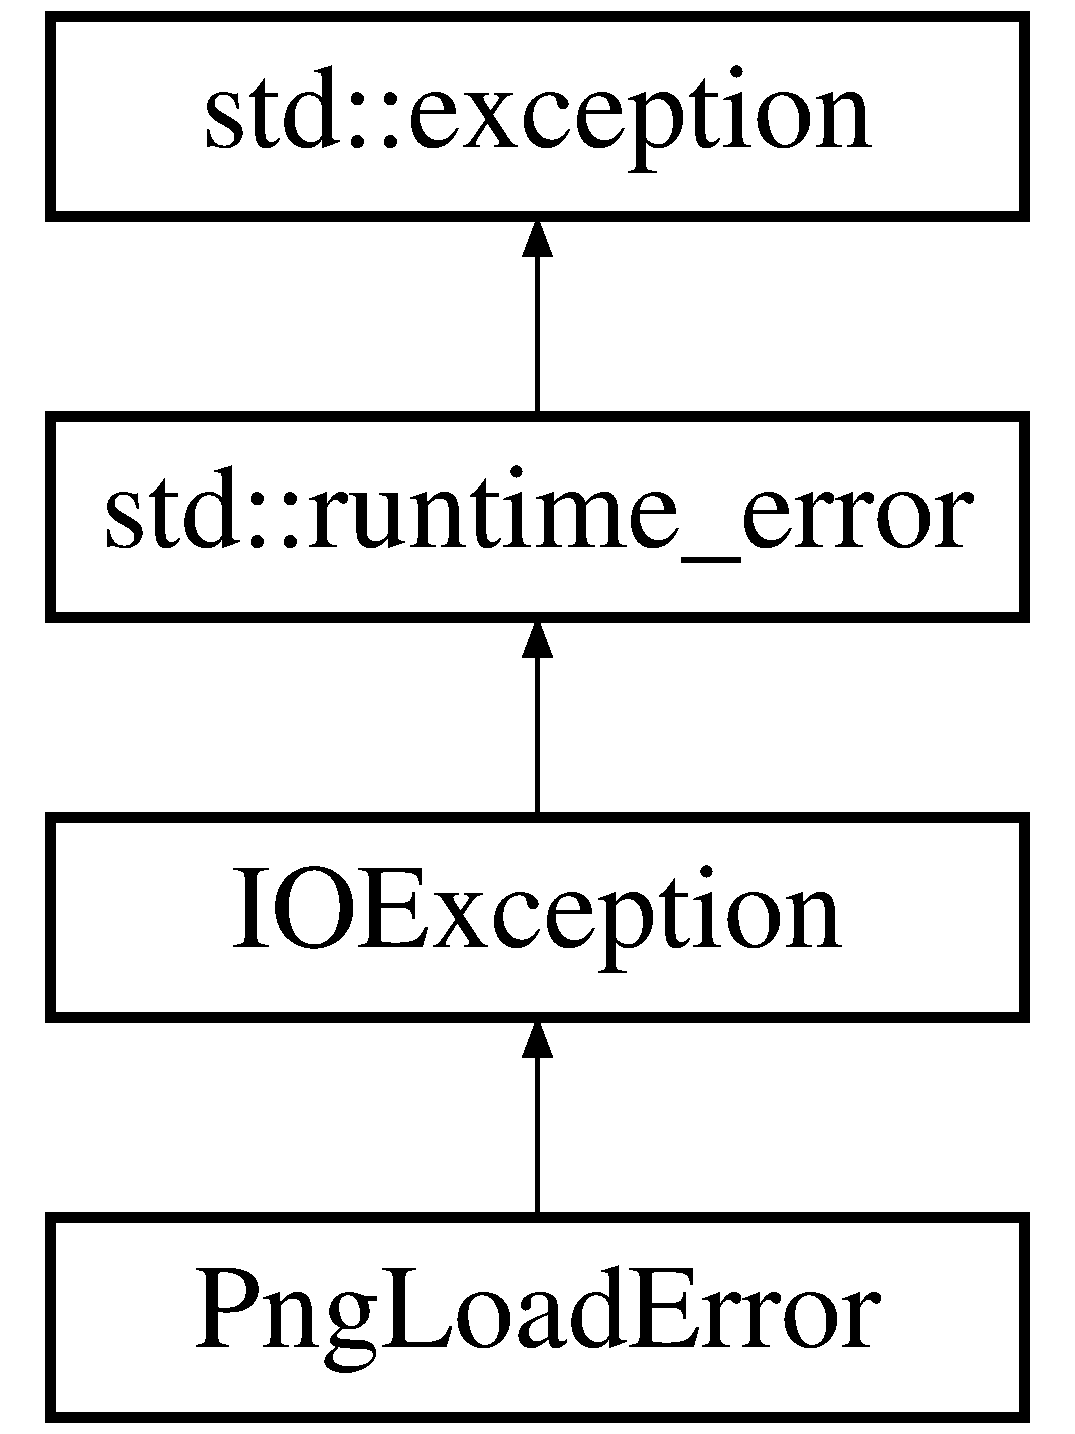
\includegraphics[height=4.000000cm]{classPngLoadError}
\end{center}
\end{figure}
\subsection*{Public Member Functions}
\begin{DoxyCompactItemize}
\item 
\hyperlink{classPngLoadError_afa477343655020d65c982aeedb118979}{Png\+Load\+Error} (const string \&arg)
\begin{DoxyCompactList}\small\item\em Write what the function does here. \end{DoxyCompactList}\end{DoxyCompactItemize}


\subsection{Detailed Description}
Write what the function does here. 

\begin{DoxyReturn}{Returns}

\end{DoxyReturn}


Definition at line 14 of file png\+\_\+decoder.\+h.



\subsection{Constructor \& Destructor Documentation}
\hypertarget{classPngLoadError_afa477343655020d65c982aeedb118979}{\index{Png\+Load\+Error@{Png\+Load\+Error}!Png\+Load\+Error@{Png\+Load\+Error}}
\index{Png\+Load\+Error@{Png\+Load\+Error}!Png\+Load\+Error@{Png\+Load\+Error}}
\subsubsection[{Png\+Load\+Error}]{\setlength{\rightskip}{0pt plus 5cm}Png\+Load\+Error\+::\+Png\+Load\+Error (
\begin{DoxyParamCaption}
\item[{const string \&}]{arg}
\end{DoxyParamCaption}
)\hspace{0.3cm}{\ttfamily [inline]}, {\ttfamily [explicit]}}}\label{classPngLoadError_afa477343655020d65c982aeedb118979}


Write what the function does here. 


\begin{DoxyParams}{Parameters}
{\em arg} & \\
\hline
\end{DoxyParams}
\begin{DoxyReturn}{Returns}

\end{DoxyReturn}


Definition at line 17 of file png\+\_\+decoder.\+h.


\begin{DoxyCode}
26             : \hyperlink{classIOException_a73fcf78b1b5820aa158680e896f0b983}{IOException}(arg)
27             \{
28             \}
\end{DoxyCode}


The documentation for this class was generated from the following file\+:\begin{DoxyCompactItemize}
\item 
png\+\_\+decoder.\+h\end{DoxyCompactItemize}

\hypertarget{structPoint}{\section{Point Struct Reference}
\label{structPoint}\index{Point@{Point}}
}
\subsection*{Public Attributes}
\begin{DoxyCompactItemize}
\item 
\hypertarget{structPoint_a05dfe2dfbde813ad234b514f30e662f1}{float {\bfseries x}}\label{structPoint_a05dfe2dfbde813ad234b514f30e662f1}

\item 
\hypertarget{structPoint_a6101960c8d2d4e8ea1d32c9234bbeb8d}{float {\bfseries y}}\label{structPoint_a6101960c8d2d4e8ea1d32c9234bbeb8d}

\end{DoxyCompactItemize}


\subsection{Detailed Description}


Definition at line 65 of file testgesture.\+c.



The documentation for this struct was generated from the following file\+:\begin{DoxyCompactItemize}
\item 
S\+D\+L2-\/2.\+0.\+3/test/testgesture.\+c\end{DoxyCompactItemize}

\hypertarget{classPointerFind}{\section{Pointer\+Find$<$ T $>$ Class Template Reference}
\label{classPointerFind}\index{Pointer\+Find$<$ T $>$@{Pointer\+Find$<$ T $>$}}
}
\subsection*{Public Member Functions}
\begin{DoxyCompactItemize}
\item 
\hypertarget{classPointerFind_a5be2db8f77c0f3f978fd0da0552fda6d}{{\bfseries Pointer\+Find} (const T \&item)}\label{classPointerFind_a5be2db8f77c0f3f978fd0da0552fda6d}

\item 
\hypertarget{classPointerFind_a726ce10f14691536e2f09b3042a9e137}{bool {\bfseries operator()} (const T $\ast$search) const }\label{classPointerFind_a726ce10f14691536e2f09b3042a9e137}

\end{DoxyCompactItemize}
\subsection*{Public Attributes}
\begin{DoxyCompactItemize}
\item 
\hypertarget{classPointerFind_a70b8fde7d321ac4a3b037c7ea8da85a5}{const T \& {\bfseries item}}\label{classPointerFind_a70b8fde7d321ac4a3b037c7ea8da85a5}

\end{DoxyCompactItemize}


\subsection{Detailed Description}
\subsubsection*{template$<$class T$>$class Pointer\+Find$<$ T $>$}



Definition at line 19 of file game.\+h.



The documentation for this class was generated from the following file\+:\begin{DoxyCompactItemize}
\item 
headers/game.\+h\end{DoxyCompactItemize}

\hypertarget{structQuitEvent}{\section{Quit\+Event Struct Reference}
\label{structQuitEvent}\index{Quit\+Event@{Quit\+Event}}
}


Write what the function does here.  




{\ttfamily \#include $<$event.\+h$>$}

Inheritance diagram for Quit\+Event\+:\begin{figure}[H]
\begin{center}
\leavevmode
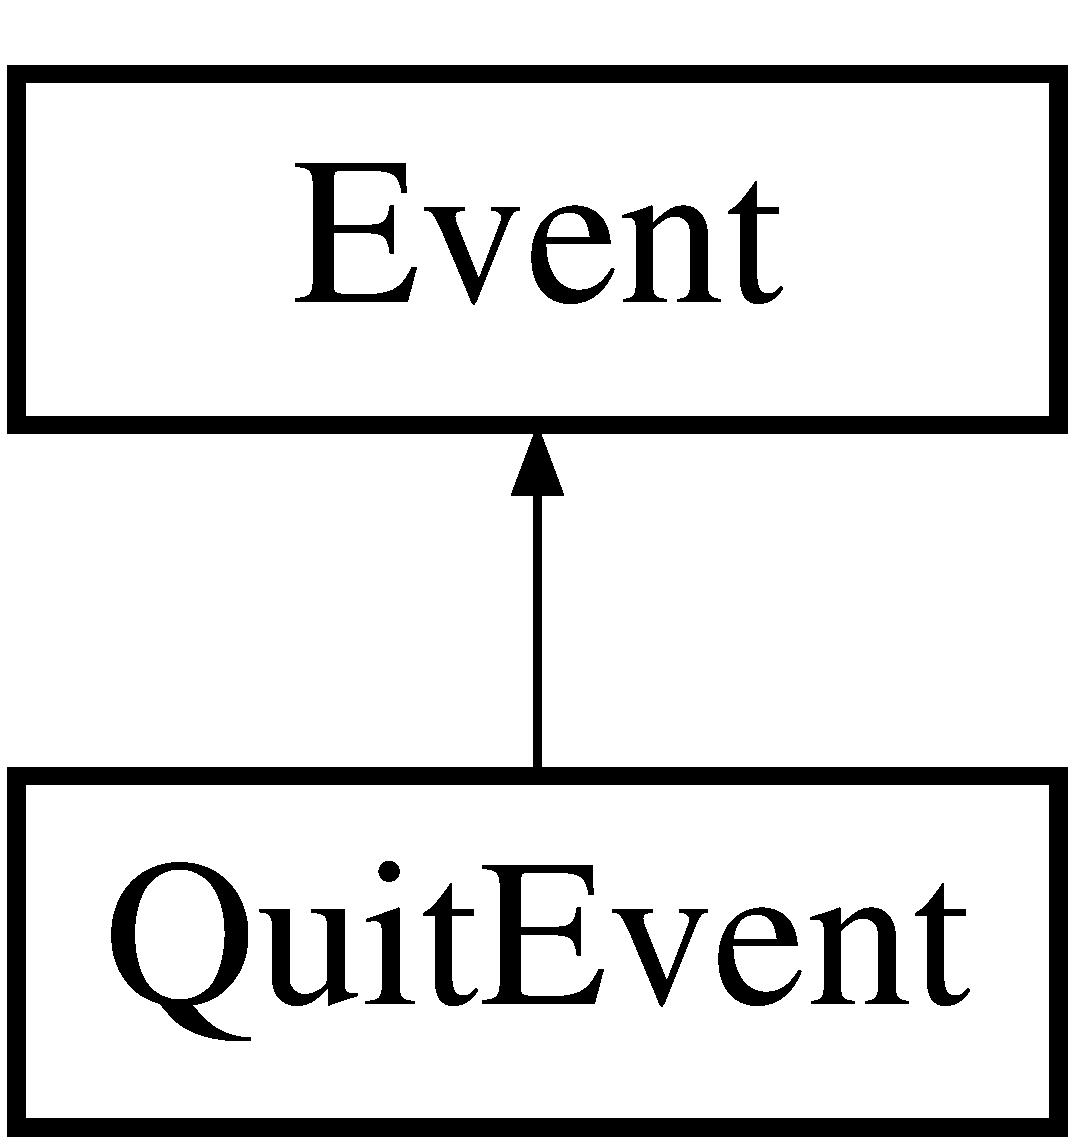
\includegraphics[height=2.000000cm]{structQuitEvent}
\end{center}
\end{figure}
\subsection*{Public Member Functions}
\begin{DoxyCompactItemize}
\item 
virtual bool \hyperlink{structQuitEvent_ac008fb404abe76e5a79741b61e59c37c}{dispatch} (shared\+\_\+ptr$<$ \hyperlink{structEventHandler}{Event\+Handler} $>$ event\+Handler) override
\begin{DoxyCompactList}\small\item\em Write what the function does here. \end{DoxyCompactList}\end{DoxyCompactItemize}
\subsection*{Additional Inherited Members}


\subsection{Detailed Description}
Write what the function does here. 


\begin{DoxyRetVals}{Return values}
{\em (variable)} & (description of variable) \\
\hline
\end{DoxyRetVals}


Definition at line 343 of file event.\+h.



\subsection{Member Function Documentation}
\hypertarget{structQuitEvent_ac008fb404abe76e5a79741b61e59c37c}{\index{Quit\+Event@{Quit\+Event}!dispatch@{dispatch}}
\index{dispatch@{dispatch}!Quit\+Event@{Quit\+Event}}
\subsubsection[{dispatch}]{\setlength{\rightskip}{0pt plus 5cm}virtual bool Quit\+Event\+::dispatch (
\begin{DoxyParamCaption}
\item[{shared\+\_\+ptr$<$ {\bf Event\+Handler} $>$}]{event\+Handler}
\end{DoxyParamCaption}
)\hspace{0.3cm}{\ttfamily [inline]}, {\ttfamily [override]}, {\ttfamily [virtual]}}}\label{structQuitEvent_ac008fb404abe76e5a79741b61e59c37c}


Write what the function does here. 


\begin{DoxyParams}{Parameters}
{\em event\+Handler} & \\
\hline
\end{DoxyParams}

\begin{DoxyRetVals}{Return values}
{\em (variable)} & (description of variable) \\
\hline
\end{DoxyRetVals}


Implements \hyperlink{classEvent}{Event}.



Definition at line 357 of file event.\+h.


\begin{DoxyCode}
358     \{
359         \textcolor{keywordflow}{return} eventHandler->handleQuit(*\textcolor{keyword}{this});
360     \}
\end{DoxyCode}


The documentation for this struct was generated from the following file\+:\begin{DoxyCompactItemize}
\item 
event.\+h\end{DoxyCompactItemize}

\hypertarget{classReader}{\section{Reader Class Reference}
\label{classReader}\index{Reader@{Reader}}
}


Write what the function does here.  




{\ttfamily \#include $<$stream.\+h$>$}

Inheritance diagram for Reader\+:\begin{figure}[H]
\begin{center}
\leavevmode
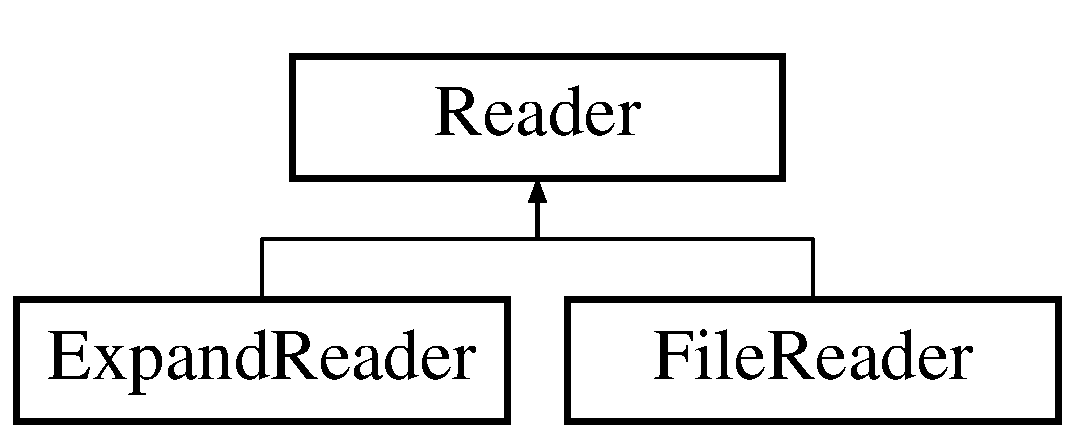
\includegraphics[height=2.000000cm]{classReader}
\end{center}
\end{figure}
\subsection*{Public Member Functions}
\begin{DoxyCompactItemize}
\item 
\hyperlink{classReader_adcda31b507720ab44044d7a21686fba2}{Reader} ()
\begin{DoxyCompactList}\small\item\em Write what the function does here. \end{DoxyCompactList}\item 
\hypertarget{classReader_a5fc83c2631c4e98ddda1eca933077ff3}{{\bfseries Reader} (const \hyperlink{classReader}{Reader} \&)=delete}\label{classReader_a5fc83c2631c4e98ddda1eca933077ff3}

\item 
\hypertarget{classReader_af0484296f2fb2a7767fdd0185a901a8a}{const \hyperlink{classReader}{Reader} \& {\bfseries operator=} (const \hyperlink{classReader}{Reader} \&)=delete}\label{classReader_af0484296f2fb2a7767fdd0185a901a8a}

\item 
virtual \hyperlink{classReader_a357153a7085f8b606de954a80411e27a}{$\sim$\+Reader} ()
\begin{DoxyCompactList}\small\item\em Write what the function does here. \end{DoxyCompactList}\item 
\hypertarget{classReader_afa26f612f949e3ddba13943e7fca7ba1}{virtual uint8\+\_\+t {\bfseries read\+Byte} ()=0}\label{classReader_afa26f612f949e3ddba13943e7fca7ba1}

\item 
void \hyperlink{classReader_a9404d9cbfc0e979836fc8870195642f7}{read\+Bytes} (uint8\+\_\+t $\ast$array, size\+\_\+t count)
\begin{DoxyCompactList}\small\item\em Write what the function does here. \end{DoxyCompactList}\item 
uint8\+\_\+t \hyperlink{classReader_a32e2703dfc40dd59216b648a0cf7ce2c}{read\+U8} ()
\begin{DoxyCompactList}\small\item\em Write what the function does here. \end{DoxyCompactList}\item 
int8\+\_\+t \hyperlink{classReader_a40f5d85934f4a635d40b91211c055c07}{read\+S8} ()
\begin{DoxyCompactList}\small\item\em Write what the function does here. \end{DoxyCompactList}\item 
uint16\+\_\+t \hyperlink{classReader_afd87a9f4420fdf4d6bd5d311c745df92}{read\+U16} ()
\begin{DoxyCompactList}\small\item\em Write what the function does here. \end{DoxyCompactList}\item 
int16\+\_\+t \hyperlink{classReader_a4039d5151950e3522a3f0bd0f8f4ebdf}{read\+S16} ()
\begin{DoxyCompactList}\small\item\em Write what the function does here. \end{DoxyCompactList}\item 
uint32\+\_\+t \hyperlink{classReader_a04653238ccdff919d98262ad99672a33}{read\+U32} ()
\begin{DoxyCompactList}\small\item\em Write what the function does here. \end{DoxyCompactList}\item 
int32\+\_\+t \hyperlink{classReader_a310529f0c2100a14b0c36abef05b9e6c}{read\+S32} ()
\begin{DoxyCompactList}\small\item\em Write what the function does here. \end{DoxyCompactList}\item 
uint64\+\_\+t \hyperlink{classReader_a43bfa733ba536d41771a56ac3e91b053}{read\+U64} ()
\begin{DoxyCompactList}\small\item\em Write what the function does here. \end{DoxyCompactList}\item 
int64\+\_\+t \hyperlink{classReader_a8fb79b338f1bbe922a0920de54159359}{read\+S64} ()
\begin{DoxyCompactList}\small\item\em Write what the function does here. \end{DoxyCompactList}\item 
float \hyperlink{classReader_ab3fb66624bda780998e0ee473a45aa0e}{read\+F32} ()
\begin{DoxyCompactList}\small\item\em Write what the function does here. \end{DoxyCompactList}\item 
double \hyperlink{classReader_a9b0ac08b982653c1ba0f6dea7e097581}{read\+F64} ()
\begin{DoxyCompactList}\small\item\em Write what the function does here. \end{DoxyCompactList}\item 
bool \hyperlink{classReader_a76fb2bc2291445a0bf1cc924e163c7f1}{read\+Bool} ()
\begin{DoxyCompactList}\small\item\em Write what the function does here. \end{DoxyCompactList}\item 
wstring \hyperlink{classReader_a4c128181d159e7581b89aa796a8de7ab}{read\+String} ()
\begin{DoxyCompactList}\small\item\em Write what the function does here. \end{DoxyCompactList}\item 
uint8\+\_\+t \hyperlink{classReader_a2996e5e74c4494fc7ae2b672fff05eb2}{read\+Limited\+U8} (uint8\+\_\+t min, uint8\+\_\+t max)
\begin{DoxyCompactList}\small\item\em Write what the function does here. \end{DoxyCompactList}\item 
int8\+\_\+t \hyperlink{classReader_aa21aee941e21f17643e826a30ba025cf}{read\+Limited\+S8} (int8\+\_\+t min, int8\+\_\+t max)
\begin{DoxyCompactList}\small\item\em Write what the function does here. \end{DoxyCompactList}\item 
uint16\+\_\+t \hyperlink{classReader_ab99b9b57b69552db10657969d3c7730e}{read\+Limited\+U16} (uint16\+\_\+t min, uint16\+\_\+t max)
\begin{DoxyCompactList}\small\item\em Write what the function does here. \end{DoxyCompactList}\item 
int16\+\_\+t \hyperlink{classReader_a3a5205e13d7346a38e713f00ad121f9b}{read\+Limited\+S16} (int16\+\_\+t min, int16\+\_\+t max)
\begin{DoxyCompactList}\small\item\em Write what the function does here. \end{DoxyCompactList}\item 
uint32\+\_\+t \hyperlink{classReader_a0fae64301d0f834b371f63ec7a14443b}{read\+Limited\+U32} (uint32\+\_\+t min, uint32\+\_\+t max)
\begin{DoxyCompactList}\small\item\em Write what the function does here. \end{DoxyCompactList}\item 
int32\+\_\+t \hyperlink{classReader_a16bf2ac6213966372fd05116fdaf7921}{read\+Limited\+S32} (int32\+\_\+t min, int32\+\_\+t max)
\begin{DoxyCompactList}\small\item\em Write what the function does here. \end{DoxyCompactList}\item 
uint64\+\_\+t \hyperlink{classReader_aba38735bda4f4fe28f865bdecb1b08a4}{read\+Limited\+U64} (uint64\+\_\+t min, uint64\+\_\+t max)
\begin{DoxyCompactList}\small\item\em Write what the function does here. \end{DoxyCompactList}\item 
int64\+\_\+t \hyperlink{classReader_a1b8e2c38eb77a67c210502642827e004}{read\+Limited\+S64} (int64\+\_\+t min, int64\+\_\+t max)
\begin{DoxyCompactList}\small\item\em Write what the function does here. \end{DoxyCompactList}\item 
float \hyperlink{classReader_ab6c81b1aa5d0f44875885bf0c7ffc147}{read\+Finite\+F32} ()
\begin{DoxyCompactList}\small\item\em Write what the function does here. \end{DoxyCompactList}\item 
double \hyperlink{classReader_a6b6d8f3a25c567d29941c496980bce4f}{read\+Finite\+F64} ()
\begin{DoxyCompactList}\small\item\em Write what the function does here. \end{DoxyCompactList}\item 
float \hyperlink{classReader_a0c4eba7401b90707776da4bab6b70d7c}{read\+Limited\+F32} (float min, float max)
\begin{DoxyCompactList}\small\item\em Write what the function does here. \end{DoxyCompactList}\item 
double \hyperlink{classReader_adabaf7ac8d6e342b6204a3c60b5c428c}{read\+Limited\+F64} (double min, double max)
\begin{DoxyCompactList}\small\item\em Write what the function does here. \end{DoxyCompactList}\end{DoxyCompactItemize}
\subsection*{Static Private Member Functions}
\begin{DoxyCompactItemize}
\item 
{\footnotesize template$<$typename T $>$ }\\static T \hyperlink{classReader_a27b3ccb94cb90cff7a6d7eb06cbb0c5c}{limit\+After\+Read} (T v, T min, T max)
\begin{DoxyCompactList}\small\item\em Write what the function does here. \end{DoxyCompactList}\end{DoxyCompactItemize}


\subsection{Detailed Description}
Write what the function does here. 

\begin{DoxyReturn}{Returns}

\end{DoxyReturn}


Definition at line 164 of file stream.\+h.



\subsection{Constructor \& Destructor Documentation}
\hypertarget{classReader_adcda31b507720ab44044d7a21686fba2}{\index{Reader@{Reader}!Reader@{Reader}}
\index{Reader@{Reader}!Reader@{Reader}}
\subsubsection[{Reader}]{\setlength{\rightskip}{0pt plus 5cm}Reader\+::\+Reader (
\begin{DoxyParamCaption}
{}
\end{DoxyParamCaption}
)\hspace{0.3cm}{\ttfamily [inline]}}}\label{classReader_adcda31b507720ab44044d7a21686fba2}


Write what the function does here. 

\begin{DoxyReturn}{Returns}

\end{DoxyReturn}


Definition at line 203 of file stream.\+h.


\begin{DoxyCode}
204         \{
205         \}
\end{DoxyCode}
\hypertarget{classReader_a357153a7085f8b606de954a80411e27a}{\index{Reader@{Reader}!````~Reader@{$\sim$\+Reader}}
\index{````~Reader@{$\sim$\+Reader}!Reader@{Reader}}
\subsubsection[{$\sim$\+Reader}]{\setlength{\rightskip}{0pt plus 5cm}virtual Reader\+::$\sim$\+Reader (
\begin{DoxyParamCaption}
{}
\end{DoxyParamCaption}
)\hspace{0.3cm}{\ttfamily [inline]}, {\ttfamily [virtual]}}}\label{classReader_a357153a7085f8b606de954a80411e27a}


Write what the function does here. 

\begin{DoxyReturn}{Returns}

\end{DoxyReturn}


Definition at line 214 of file stream.\+h.


\begin{DoxyCode}
215         \{
216         \}
\end{DoxyCode}


\subsection{Member Function Documentation}
\hypertarget{classReader_a27b3ccb94cb90cff7a6d7eb06cbb0c5c}{\index{Reader@{Reader}!limit\+After\+Read@{limit\+After\+Read}}
\index{limit\+After\+Read@{limit\+After\+Read}!Reader@{Reader}}
\subsubsection[{limit\+After\+Read}]{\setlength{\rightskip}{0pt plus 5cm}template$<$typename T $>$ static T Reader\+::limit\+After\+Read (
\begin{DoxyParamCaption}
\item[{T}]{v, }
\item[{T}]{min, }
\item[{T}]{max}
\end{DoxyParamCaption}
)\hspace{0.3cm}{\ttfamily [inline]}, {\ttfamily [static]}, {\ttfamily [private]}}}\label{classReader_a27b3ccb94cb90cff7a6d7eb06cbb0c5c}


Write what the function does here. 


\begin{DoxyParams}{Parameters}
{\em v} & \\
\hline
{\em min} & \\
\hline
{\em max} & \\
\hline
\end{DoxyParams}
\begin{DoxyReturn}{Returns}

\end{DoxyReturn}
Write what the function does here


\begin{DoxyParams}{Parameters}
{\em max} & \\
\hline
\end{DoxyParams}
\begin{DoxyReturn}{Returns}

\end{DoxyReturn}


Definition at line 178 of file stream.\+h.


\begin{DoxyCode}
179             \{
180 \textcolor{comment}{}
181 \textcolor{comment}{                /**}
182 \textcolor{comment}{                 * @brief Write what the function does here}
183 \textcolor{comment}{                 *}
184 \textcolor{comment}{                 * @param max}
185 \textcolor{comment}{                 *}
186 \textcolor{comment}{                 * @return}
187 \textcolor{comment}{                 **/}
188                 \textcolor{keywordflow}{if}(v < min || v > max)
189                 \{
190                     ostringstream os;
191                     os << \textcolor{stringliteral}{"read value out of range : "} << v;
192                     \textcolor{keywordflow}{throw} \hyperlink{classInvalidDataValueException}{InvalidDataValueException}(os.str());
193                 \}
194                 \textcolor{keywordflow}{return} v;
195             \}
\end{DoxyCode}
\hypertarget{classReader_a76fb2bc2291445a0bf1cc924e163c7f1}{\index{Reader@{Reader}!read\+Bool@{read\+Bool}}
\index{read\+Bool@{read\+Bool}!Reader@{Reader}}
\subsubsection[{read\+Bool}]{\setlength{\rightskip}{0pt plus 5cm}bool Reader\+::read\+Bool (
\begin{DoxyParamCaption}
{}
\end{DoxyParamCaption}
)\hspace{0.3cm}{\ttfamily [inline]}}}\label{classReader_a76fb2bc2291445a0bf1cc924e163c7f1}


Write what the function does here. 

\begin{DoxyReturn}{Returns}

\end{DoxyReturn}


Definition at line 393 of file stream.\+h.


\begin{DoxyCode}
394         \{
395             \textcolor{keywordflow}{return} \hyperlink{classReader_a32e2703dfc40dd59216b648a0cf7ce2c}{readU8}() != 0;
396         \}
\end{DoxyCode}
\hypertarget{classReader_a9404d9cbfc0e979836fc8870195642f7}{\index{Reader@{Reader}!read\+Bytes@{read\+Bytes}}
\index{read\+Bytes@{read\+Bytes}!Reader@{Reader}}
\subsubsection[{read\+Bytes}]{\setlength{\rightskip}{0pt plus 5cm}void Reader\+::read\+Bytes (
\begin{DoxyParamCaption}
\item[{uint8\+\_\+t $\ast$}]{array, }
\item[{size\+\_\+t}]{count}
\end{DoxyParamCaption}
)\hspace{0.3cm}{\ttfamily [inline]}}}\label{classReader_a9404d9cbfc0e979836fc8870195642f7}


Write what the function does here. 


\begin{DoxyParams}{Parameters}
{\em array} & \\
\hline
{\em count} & \\
\hline
\end{DoxyParams}
Write what the function does here

\begin{DoxyReturn}{Returns}

\end{DoxyReturn}


Definition at line 225 of file stream.\+h.


\begin{DoxyCode}
226         \{
227 \textcolor{comment}{}
228 \textcolor{comment}{            /**}
229 \textcolor{comment}{             * @brief Write what the function does here}
230 \textcolor{comment}{             *}
231 \textcolor{comment}{             * @return}
232 \textcolor{comment}{             **/}
233             \textcolor{keywordflow}{for}(\textcolor{keywordtype}{size\_t} i = 0; i < count; i++)
234             \{
235                 array[i] = readByte();
236             \}
237         \}
\end{DoxyCode}
\hypertarget{classReader_ab3fb66624bda780998e0ee473a45aa0e}{\index{Reader@{Reader}!read\+F32@{read\+F32}}
\index{read\+F32@{read\+F32}!Reader@{Reader}}
\subsubsection[{read\+F32}]{\setlength{\rightskip}{0pt plus 5cm}float Reader\+::read\+F32 (
\begin{DoxyParamCaption}
{}
\end{DoxyParamCaption}
)\hspace{0.3cm}{\ttfamily [inline]}}}\label{classReader_ab3fb66624bda780998e0ee473a45aa0e}


Write what the function does here. 

\begin{DoxyReturn}{Returns}

\end{DoxyReturn}
Write what the function does here

\begin{DoxyReturn}{Returns}

\end{DoxyReturn}


Definition at line 343 of file stream.\+h.


\begin{DoxyCode}
344         \{
345             static\_assert(\textcolor{keyword}{sizeof}(\textcolor{keywordtype}{float}) == \textcolor{keyword}{sizeof}(uint32\_t), \textcolor{stringliteral}{"float is not 32 bits"});
346 \textcolor{comment}{}
347 \textcolor{comment}{            /**}
348 \textcolor{comment}{             * @brief Write what the function does here}
349 \textcolor{comment}{             *}
350 \textcolor{comment}{             * @return}
351 \textcolor{comment}{             **/}
352             \textcolor{keyword}{union}
353             \{
354                 uint32\_t ival;
355                 \textcolor{keywordtype}{float} fval;
356             \};
357             ival = \hyperlink{classReader_a04653238ccdff919d98262ad99672a33}{readU32}();
358             \textcolor{keywordtype}{float} retval = fval;
359             DUMP\_V(\hyperlink{classReader_ab3fb66624bda780998e0ee473a45aa0e}{readF32}, retval);
360             \textcolor{keywordflow}{return} retval;
361         \}
\end{DoxyCode}
\hypertarget{classReader_a9b0ac08b982653c1ba0f6dea7e097581}{\index{Reader@{Reader}!read\+F64@{read\+F64}}
\index{read\+F64@{read\+F64}!Reader@{Reader}}
\subsubsection[{read\+F64}]{\setlength{\rightskip}{0pt plus 5cm}double Reader\+::read\+F64 (
\begin{DoxyParamCaption}
{}
\end{DoxyParamCaption}
)\hspace{0.3cm}{\ttfamily [inline]}}}\label{classReader_a9b0ac08b982653c1ba0f6dea7e097581}


Write what the function does here. 

\begin{DoxyReturn}{Returns}

\end{DoxyReturn}
Write what the function does here

\begin{DoxyReturn}{Returns}

\end{DoxyReturn}


Definition at line 368 of file stream.\+h.


\begin{DoxyCode}
369         \{
370             static\_assert(\textcolor{keyword}{sizeof}(\textcolor{keywordtype}{double}) == \textcolor{keyword}{sizeof}(uint64\_t), \textcolor{stringliteral}{"double is not 64 bits"});
371 \textcolor{comment}{}
372 \textcolor{comment}{            /**}
373 \textcolor{comment}{             * @brief Write what the function does here}
374 \textcolor{comment}{             *}
375 \textcolor{comment}{             * @return}
376 \textcolor{comment}{             **/}
377             \textcolor{keyword}{union}
378             \{
379                 uint64\_t ival;
380                 \textcolor{keywordtype}{double} fval;
381             \};
382             ival = \hyperlink{classReader_a43bfa733ba536d41771a56ac3e91b053}{readU64}();
383             \textcolor{keywordtype}{double} retval = fval;
384             DUMP\_V(\hyperlink{classReader_a9b0ac08b982653c1ba0f6dea7e097581}{readF64}, retval);
385             \textcolor{keywordflow}{return} retval;
386         \}
\end{DoxyCode}
\hypertarget{classReader_ab6c81b1aa5d0f44875885bf0c7ffc147}{\index{Reader@{Reader}!read\+Finite\+F32@{read\+Finite\+F32}}
\index{read\+Finite\+F32@{read\+Finite\+F32}!Reader@{Reader}}
\subsubsection[{read\+Finite\+F32}]{\setlength{\rightskip}{0pt plus 5cm}float Reader\+::read\+Finite\+F32 (
\begin{DoxyParamCaption}
{}
\end{DoxyParamCaption}
)\hspace{0.3cm}{\ttfamily [inline]}}}\label{classReader_ab6c81b1aa5d0f44875885bf0c7ffc147}


Write what the function does here. 

\begin{DoxyReturn}{Returns}

\end{DoxyReturn}
Write what the function does here


\begin{DoxyParams}{Parameters}
{\em retval} & \\
\hline
\end{DoxyParams}
\begin{DoxyReturn}{Returns}

\end{DoxyReturn}


Definition at line 623 of file stream.\+h.


\begin{DoxyCode}
624         \{
625             \textcolor{keywordtype}{float} retval = \hyperlink{classReader_ab3fb66624bda780998e0ee473a45aa0e}{readF32}();
626 \textcolor{comment}{}
627 \textcolor{comment}{            /**}
628 \textcolor{comment}{             * @brief Write what the function does here}
629 \textcolor{comment}{             *}
630 \textcolor{comment}{             * @param retval}
631 \textcolor{comment}{             *}
632 \textcolor{comment}{             * @return}
633 \textcolor{comment}{             **/}
634             \textcolor{keywordflow}{if}(!isfinite(retval))
635             \{
636                 \textcolor{keywordflow}{throw} \hyperlink{classInvalidDataValueException}{InvalidDataValueException}(\textcolor{stringliteral}{"read value is not finite"});
637             \}
638             \textcolor{keywordflow}{return} retval;
639         \}
\end{DoxyCode}
\hypertarget{classReader_a6b6d8f3a25c567d29941c496980bce4f}{\index{Reader@{Reader}!read\+Finite\+F64@{read\+Finite\+F64}}
\index{read\+Finite\+F64@{read\+Finite\+F64}!Reader@{Reader}}
\subsubsection[{read\+Finite\+F64}]{\setlength{\rightskip}{0pt plus 5cm}double Reader\+::read\+Finite\+F64 (
\begin{DoxyParamCaption}
{}
\end{DoxyParamCaption}
)\hspace{0.3cm}{\ttfamily [inline]}}}\label{classReader_a6b6d8f3a25c567d29941c496980bce4f}


Write what the function does here. 

\begin{DoxyReturn}{Returns}

\end{DoxyReturn}
Write what the function does here


\begin{DoxyParams}{Parameters}
{\em retval} & \\
\hline
\end{DoxyParams}
\begin{DoxyReturn}{Returns}

\end{DoxyReturn}


Definition at line 646 of file stream.\+h.


\begin{DoxyCode}
647         \{
648             \textcolor{keywordtype}{double} retval = \hyperlink{classReader_a9b0ac08b982653c1ba0f6dea7e097581}{readF64}();
649 \textcolor{comment}{}
650 \textcolor{comment}{            /**}
651 \textcolor{comment}{             * @brief Write what the function does here}
652 \textcolor{comment}{             *}
653 \textcolor{comment}{             * @param retval}
654 \textcolor{comment}{             *}
655 \textcolor{comment}{             * @return}
656 \textcolor{comment}{             **/}
657             \textcolor{keywordflow}{if}(!isfinite(retval))
658             \{
659                 \textcolor{keywordflow}{throw} \hyperlink{classInvalidDataValueException}{InvalidDataValueException}(\textcolor{stringliteral}{"read value is not finite"});
660             \}
661             \textcolor{keywordflow}{return} retval;
662         \}
\end{DoxyCode}
\hypertarget{classReader_a0c4eba7401b90707776da4bab6b70d7c}{\index{Reader@{Reader}!read\+Limited\+F32@{read\+Limited\+F32}}
\index{read\+Limited\+F32@{read\+Limited\+F32}!Reader@{Reader}}
\subsubsection[{read\+Limited\+F32}]{\setlength{\rightskip}{0pt plus 5cm}float Reader\+::read\+Limited\+F32 (
\begin{DoxyParamCaption}
\item[{float}]{min, }
\item[{float}]{max}
\end{DoxyParamCaption}
)\hspace{0.3cm}{\ttfamily [inline]}}}\label{classReader_a0c4eba7401b90707776da4bab6b70d7c}


Write what the function does here. 


\begin{DoxyParams}{Parameters}
{\em min} & \\
\hline
{\em max} & \\
\hline
\end{DoxyParams}
\begin{DoxyReturn}{Returns}

\end{DoxyReturn}


Definition at line 672 of file stream.\+h.


\begin{DoxyCode}
673         \{
674             \textcolor{keywordflow}{return} \hyperlink{classReader_a27b3ccb94cb90cff7a6d7eb06cbb0c5c}{limitAfterRead}(\hyperlink{classReader_ab6c81b1aa5d0f44875885bf0c7ffc147}{readFiniteF32}(), min, max);
675         \}
\end{DoxyCode}
\hypertarget{classReader_adabaf7ac8d6e342b6204a3c60b5c428c}{\index{Reader@{Reader}!read\+Limited\+F64@{read\+Limited\+F64}}
\index{read\+Limited\+F64@{read\+Limited\+F64}!Reader@{Reader}}
\subsubsection[{read\+Limited\+F64}]{\setlength{\rightskip}{0pt plus 5cm}double Reader\+::read\+Limited\+F64 (
\begin{DoxyParamCaption}
\item[{double}]{min, }
\item[{double}]{max}
\end{DoxyParamCaption}
)\hspace{0.3cm}{\ttfamily [inline]}}}\label{classReader_adabaf7ac8d6e342b6204a3c60b5c428c}


Write what the function does here. 


\begin{DoxyParams}{Parameters}
{\em min} & \\
\hline
{\em max} & \\
\hline
\end{DoxyParams}
\begin{DoxyReturn}{Returns}

\end{DoxyReturn}


Definition at line 685 of file stream.\+h.


\begin{DoxyCode}
686         \{
687             \textcolor{keywordflow}{return} \hyperlink{classReader_a27b3ccb94cb90cff7a6d7eb06cbb0c5c}{limitAfterRead}(\hyperlink{classReader_a6b6d8f3a25c567d29941c496980bce4f}{readFiniteF64}(), min, max);
688         \}
\end{DoxyCode}
\hypertarget{classReader_a3a5205e13d7346a38e713f00ad121f9b}{\index{Reader@{Reader}!read\+Limited\+S16@{read\+Limited\+S16}}
\index{read\+Limited\+S16@{read\+Limited\+S16}!Reader@{Reader}}
\subsubsection[{read\+Limited\+S16}]{\setlength{\rightskip}{0pt plus 5cm}int16\+\_\+t Reader\+::read\+Limited\+S16 (
\begin{DoxyParamCaption}
\item[{int16\+\_\+t}]{min, }
\item[{int16\+\_\+t}]{max}
\end{DoxyParamCaption}
)\hspace{0.3cm}{\ttfamily [inline]}}}\label{classReader_a3a5205e13d7346a38e713f00ad121f9b}


Write what the function does here. 


\begin{DoxyParams}{Parameters}
{\em min} & \\
\hline
{\em max} & \\
\hline
\end{DoxyParams}
\begin{DoxyReturn}{Returns}

\end{DoxyReturn}


Definition at line 561 of file stream.\+h.


\begin{DoxyCode}
562         \{
563             \textcolor{keywordflow}{return} \hyperlink{classReader_a27b3ccb94cb90cff7a6d7eb06cbb0c5c}{limitAfterRead}(\hyperlink{classReader_a4039d5151950e3522a3f0bd0f8f4ebdf}{readS16}(), min, max);
564         \}
\end{DoxyCode}
\hypertarget{classReader_a16bf2ac6213966372fd05116fdaf7921}{\index{Reader@{Reader}!read\+Limited\+S32@{read\+Limited\+S32}}
\index{read\+Limited\+S32@{read\+Limited\+S32}!Reader@{Reader}}
\subsubsection[{read\+Limited\+S32}]{\setlength{\rightskip}{0pt plus 5cm}int32\+\_\+t Reader\+::read\+Limited\+S32 (
\begin{DoxyParamCaption}
\item[{int32\+\_\+t}]{min, }
\item[{int32\+\_\+t}]{max}
\end{DoxyParamCaption}
)\hspace{0.3cm}{\ttfamily [inline]}}}\label{classReader_a16bf2ac6213966372fd05116fdaf7921}


Write what the function does here. 


\begin{DoxyParams}{Parameters}
{\em min} & \\
\hline
{\em max} & \\
\hline
\end{DoxyParams}
\begin{DoxyReturn}{Returns}

\end{DoxyReturn}


Definition at line 587 of file stream.\+h.


\begin{DoxyCode}
588         \{
589             \textcolor{keywordflow}{return} \hyperlink{classReader_a27b3ccb94cb90cff7a6d7eb06cbb0c5c}{limitAfterRead}(\hyperlink{classReader_a310529f0c2100a14b0c36abef05b9e6c}{readS32}(), min, max);
590         \}
\end{DoxyCode}
\hypertarget{classReader_a1b8e2c38eb77a67c210502642827e004}{\index{Reader@{Reader}!read\+Limited\+S64@{read\+Limited\+S64}}
\index{read\+Limited\+S64@{read\+Limited\+S64}!Reader@{Reader}}
\subsubsection[{read\+Limited\+S64}]{\setlength{\rightskip}{0pt plus 5cm}int64\+\_\+t Reader\+::read\+Limited\+S64 (
\begin{DoxyParamCaption}
\item[{int64\+\_\+t}]{min, }
\item[{int64\+\_\+t}]{max}
\end{DoxyParamCaption}
)\hspace{0.3cm}{\ttfamily [inline]}}}\label{classReader_a1b8e2c38eb77a67c210502642827e004}


Write what the function does here. 


\begin{DoxyParams}{Parameters}
{\em min} & \\
\hline
{\em max} & \\
\hline
\end{DoxyParams}
\begin{DoxyReturn}{Returns}

\end{DoxyReturn}


Definition at line 613 of file stream.\+h.


\begin{DoxyCode}
614         \{
615             \textcolor{keywordflow}{return} \hyperlink{classReader_a27b3ccb94cb90cff7a6d7eb06cbb0c5c}{limitAfterRead}(\hyperlink{classReader_a8fb79b338f1bbe922a0920de54159359}{readS64}(), min, max);
616         \}
\end{DoxyCode}
\hypertarget{classReader_aa21aee941e21f17643e826a30ba025cf}{\index{Reader@{Reader}!read\+Limited\+S8@{read\+Limited\+S8}}
\index{read\+Limited\+S8@{read\+Limited\+S8}!Reader@{Reader}}
\subsubsection[{read\+Limited\+S8}]{\setlength{\rightskip}{0pt plus 5cm}int8\+\_\+t Reader\+::read\+Limited\+S8 (
\begin{DoxyParamCaption}
\item[{int8\+\_\+t}]{min, }
\item[{int8\+\_\+t}]{max}
\end{DoxyParamCaption}
)\hspace{0.3cm}{\ttfamily [inline]}}}\label{classReader_aa21aee941e21f17643e826a30ba025cf}


Write what the function does here. 


\begin{DoxyParams}{Parameters}
{\em min} & \\
\hline
{\em max} & \\
\hline
\end{DoxyParams}
\begin{DoxyReturn}{Returns}

\end{DoxyReturn}


Definition at line 535 of file stream.\+h.


\begin{DoxyCode}
536         \{
537             \textcolor{keywordflow}{return} \hyperlink{classReader_a27b3ccb94cb90cff7a6d7eb06cbb0c5c}{limitAfterRead}(\hyperlink{classReader_a40f5d85934f4a635d40b91211c055c07}{readS8}(), min, max);
538         \}
\end{DoxyCode}
\hypertarget{classReader_ab99b9b57b69552db10657969d3c7730e}{\index{Reader@{Reader}!read\+Limited\+U16@{read\+Limited\+U16}}
\index{read\+Limited\+U16@{read\+Limited\+U16}!Reader@{Reader}}
\subsubsection[{read\+Limited\+U16}]{\setlength{\rightskip}{0pt plus 5cm}uint16\+\_\+t Reader\+::read\+Limited\+U16 (
\begin{DoxyParamCaption}
\item[{uint16\+\_\+t}]{min, }
\item[{uint16\+\_\+t}]{max}
\end{DoxyParamCaption}
)\hspace{0.3cm}{\ttfamily [inline]}}}\label{classReader_ab99b9b57b69552db10657969d3c7730e}


Write what the function does here. 


\begin{DoxyParams}{Parameters}
{\em min} & \\
\hline
{\em max} & \\
\hline
\end{DoxyParams}
\begin{DoxyReturn}{Returns}

\end{DoxyReturn}


Definition at line 548 of file stream.\+h.


\begin{DoxyCode}
549         \{
550             \textcolor{keywordflow}{return} \hyperlink{classReader_a27b3ccb94cb90cff7a6d7eb06cbb0c5c}{limitAfterRead}(\hyperlink{classReader_afd87a9f4420fdf4d6bd5d311c745df92}{readU16}(), min, max);
551         \}
\end{DoxyCode}
\hypertarget{classReader_a0fae64301d0f834b371f63ec7a14443b}{\index{Reader@{Reader}!read\+Limited\+U32@{read\+Limited\+U32}}
\index{read\+Limited\+U32@{read\+Limited\+U32}!Reader@{Reader}}
\subsubsection[{read\+Limited\+U32}]{\setlength{\rightskip}{0pt plus 5cm}uint32\+\_\+t Reader\+::read\+Limited\+U32 (
\begin{DoxyParamCaption}
\item[{uint32\+\_\+t}]{min, }
\item[{uint32\+\_\+t}]{max}
\end{DoxyParamCaption}
)\hspace{0.3cm}{\ttfamily [inline]}}}\label{classReader_a0fae64301d0f834b371f63ec7a14443b}


Write what the function does here. 


\begin{DoxyParams}{Parameters}
{\em min} & \\
\hline
{\em max} & \\
\hline
\end{DoxyParams}
\begin{DoxyReturn}{Returns}

\end{DoxyReturn}


Definition at line 574 of file stream.\+h.


\begin{DoxyCode}
575         \{
576             \textcolor{keywordflow}{return} \hyperlink{classReader_a27b3ccb94cb90cff7a6d7eb06cbb0c5c}{limitAfterRead}(\hyperlink{classReader_a04653238ccdff919d98262ad99672a33}{readU32}(), min, max);
577         \}
\end{DoxyCode}
\hypertarget{classReader_aba38735bda4f4fe28f865bdecb1b08a4}{\index{Reader@{Reader}!read\+Limited\+U64@{read\+Limited\+U64}}
\index{read\+Limited\+U64@{read\+Limited\+U64}!Reader@{Reader}}
\subsubsection[{read\+Limited\+U64}]{\setlength{\rightskip}{0pt plus 5cm}uint64\+\_\+t Reader\+::read\+Limited\+U64 (
\begin{DoxyParamCaption}
\item[{uint64\+\_\+t}]{min, }
\item[{uint64\+\_\+t}]{max}
\end{DoxyParamCaption}
)\hspace{0.3cm}{\ttfamily [inline]}}}\label{classReader_aba38735bda4f4fe28f865bdecb1b08a4}


Write what the function does here. 


\begin{DoxyParams}{Parameters}
{\em min} & \\
\hline
{\em max} & \\
\hline
\end{DoxyParams}
\begin{DoxyReturn}{Returns}

\end{DoxyReturn}


Definition at line 600 of file stream.\+h.


\begin{DoxyCode}
601         \{
602             \textcolor{keywordflow}{return} \hyperlink{classReader_a27b3ccb94cb90cff7a6d7eb06cbb0c5c}{limitAfterRead}(\hyperlink{classReader_a43bfa733ba536d41771a56ac3e91b053}{readU64}(), min, max);
603         \}
\end{DoxyCode}
\hypertarget{classReader_a2996e5e74c4494fc7ae2b672fff05eb2}{\index{Reader@{Reader}!read\+Limited\+U8@{read\+Limited\+U8}}
\index{read\+Limited\+U8@{read\+Limited\+U8}!Reader@{Reader}}
\subsubsection[{read\+Limited\+U8}]{\setlength{\rightskip}{0pt plus 5cm}uint8\+\_\+t Reader\+::read\+Limited\+U8 (
\begin{DoxyParamCaption}
\item[{uint8\+\_\+t}]{min, }
\item[{uint8\+\_\+t}]{max}
\end{DoxyParamCaption}
)\hspace{0.3cm}{\ttfamily [inline]}}}\label{classReader_a2996e5e74c4494fc7ae2b672fff05eb2}


Write what the function does here. 


\begin{DoxyParams}{Parameters}
{\em min} & \\
\hline
{\em max} & \\
\hline
\end{DoxyParams}
\begin{DoxyReturn}{Returns}

\end{DoxyReturn}


Definition at line 522 of file stream.\+h.


\begin{DoxyCode}
523         \{
524             \textcolor{keywordflow}{return} \hyperlink{classReader_a27b3ccb94cb90cff7a6d7eb06cbb0c5c}{limitAfterRead}(\hyperlink{classReader_a32e2703dfc40dd59216b648a0cf7ce2c}{readU8}(), min, max);
525         \}
\end{DoxyCode}
\hypertarget{classReader_a4039d5151950e3522a3f0bd0f8f4ebdf}{\index{Reader@{Reader}!read\+S16@{read\+S16}}
\index{read\+S16@{read\+S16}!Reader@{Reader}}
\subsubsection[{read\+S16}]{\setlength{\rightskip}{0pt plus 5cm}int16\+\_\+t Reader\+::read\+S16 (
\begin{DoxyParamCaption}
{}
\end{DoxyParamCaption}
)\hspace{0.3cm}{\ttfamily [inline]}}}\label{classReader_a4039d5151950e3522a3f0bd0f8f4ebdf}


Write what the function does here. 

\begin{DoxyReturn}{Returns}

\end{DoxyReturn}


Definition at line 281 of file stream.\+h.


\begin{DoxyCode}
282         \{
283             int16\_t retval = \hyperlink{classReader_afd87a9f4420fdf4d6bd5d311c745df92}{readU16}();
284             DUMP\_V(\hyperlink{classReader_a4039d5151950e3522a3f0bd0f8f4ebdf}{readS16}, retval);
285             \textcolor{keywordflow}{return} retval;
286         \}
\end{DoxyCode}
\hypertarget{classReader_a310529f0c2100a14b0c36abef05b9e6c}{\index{Reader@{Reader}!read\+S32@{read\+S32}}
\index{read\+S32@{read\+S32}!Reader@{Reader}}
\subsubsection[{read\+S32}]{\setlength{\rightskip}{0pt plus 5cm}int32\+\_\+t Reader\+::read\+S32 (
\begin{DoxyParamCaption}
{}
\end{DoxyParamCaption}
)\hspace{0.3cm}{\ttfamily [inline]}}}\label{classReader_a310529f0c2100a14b0c36abef05b9e6c}


Write what the function does here. 

\begin{DoxyReturn}{Returns}

\end{DoxyReturn}


Definition at line 306 of file stream.\+h.


\begin{DoxyCode}
307         \{
308             int32\_t retval = \hyperlink{classReader_a04653238ccdff919d98262ad99672a33}{readU32}();
309             DUMP\_V(\hyperlink{classReader_a310529f0c2100a14b0c36abef05b9e6c}{readS32}, retval);
310             \textcolor{keywordflow}{return} retval;
311         \}
\end{DoxyCode}
\hypertarget{classReader_a8fb79b338f1bbe922a0920de54159359}{\index{Reader@{Reader}!read\+S64@{read\+S64}}
\index{read\+S64@{read\+S64}!Reader@{Reader}}
\subsubsection[{read\+S64}]{\setlength{\rightskip}{0pt plus 5cm}int64\+\_\+t Reader\+::read\+S64 (
\begin{DoxyParamCaption}
{}
\end{DoxyParamCaption}
)\hspace{0.3cm}{\ttfamily [inline]}}}\label{classReader_a8fb79b338f1bbe922a0920de54159359}


Write what the function does here. 

\begin{DoxyReturn}{Returns}

\end{DoxyReturn}


Definition at line 331 of file stream.\+h.


\begin{DoxyCode}
332         \{
333             int64\_t retval = \hyperlink{classReader_a43bfa733ba536d41771a56ac3e91b053}{readU64}();
334             DUMP\_V(\hyperlink{classReader_a8fb79b338f1bbe922a0920de54159359}{readS64}, retval);
335             \textcolor{keywordflow}{return} retval;
336         \}
\end{DoxyCode}
\hypertarget{classReader_a40f5d85934f4a635d40b91211c055c07}{\index{Reader@{Reader}!read\+S8@{read\+S8}}
\index{read\+S8@{read\+S8}!Reader@{Reader}}
\subsubsection[{read\+S8}]{\setlength{\rightskip}{0pt plus 5cm}int8\+\_\+t Reader\+::read\+S8 (
\begin{DoxyParamCaption}
{}
\end{DoxyParamCaption}
)\hspace{0.3cm}{\ttfamily [inline]}}}\label{classReader_a40f5d85934f4a635d40b91211c055c07}


Write what the function does here. 

\begin{DoxyReturn}{Returns}

\end{DoxyReturn}


Definition at line 256 of file stream.\+h.


\begin{DoxyCode}
257         \{
258             int8\_t retval = readByte();
259             DUMP\_V(\hyperlink{classReader_a40f5d85934f4a635d40b91211c055c07}{readS8}, (\textcolor{keywordtype}{int})retval);
260             \textcolor{keywordflow}{return} retval;
261         \}
\end{DoxyCode}
\hypertarget{classReader_a4c128181d159e7581b89aa796a8de7ab}{\index{Reader@{Reader}!read\+String@{read\+String}}
\index{read\+String@{read\+String}!Reader@{Reader}}
\subsubsection[{read\+String}]{\setlength{\rightskip}{0pt plus 5cm}wstring Reader\+::read\+String (
\begin{DoxyParamCaption}
{}
\end{DoxyParamCaption}
)\hspace{0.3cm}{\ttfamily [inline]}}}\label{classReader_a4c128181d159e7581b89aa796a8de7ab}


Write what the function does here. 

\begin{DoxyReturn}{Returns}

\end{DoxyReturn}
Write what the function does here

\begin{DoxyReturn}{Returns}

\end{DoxyReturn}
Write what the function does here


\begin{DoxyParams}{Parameters}
{\em 0} & \\
\hline
\end{DoxyParams}
\begin{DoxyReturn}{Returns}

\end{DoxyReturn}
Write what the function does here


\begin{DoxyParams}{Parameters}
{\em 0x80} & \\
\hline
{\em 0} & \\
\hline
\end{DoxyParams}
\begin{DoxyReturn}{Returns}

\end{DoxyReturn}
Write what the function does here


\begin{DoxyParams}{Parameters}
{\em 0x\+E0} & \\
\hline
{\em 0x\+C0} & \\
\hline
\end{DoxyParams}
\begin{DoxyReturn}{Returns}

\end{DoxyReturn}
Write what the function does here


\begin{DoxyParams}{Parameters}
{\em 0x\+F0} & \\
\hline
{\em 0x\+E0} & \\
\hline
\end{DoxyParams}
\begin{DoxyReturn}{Returns}

\end{DoxyReturn}
Write what the function does here


\begin{DoxyParams}{Parameters}
{\em 0x\+F8} & \\
\hline
{\em 0x\+F0} & \\
\hline
\end{DoxyParams}
\begin{DoxyReturn}{Returns}

\end{DoxyReturn}


Definition at line 403 of file stream.\+h.


\begin{DoxyCode}
404         \{
405             wstring retval = L\textcolor{stringliteral}{""};
406 \textcolor{comment}{}
407 \textcolor{comment}{            /**}
408 \textcolor{comment}{             * @brief Write what the function does here}
409 \textcolor{comment}{             *}
410 \textcolor{comment}{             * @return}
411 \textcolor{comment}{             **/}
412             \textcolor{keywordflow}{for}(;;)
413             \{
414                 uint32\_t b1 = \hyperlink{classReader_a32e2703dfc40dd59216b648a0cf7ce2c}{readU8}();
415 \textcolor{comment}{}
416 \textcolor{comment}{                /**}
417 \textcolor{comment}{                 * @brief Write what the function does here}
418 \textcolor{comment}{                 *}
419 \textcolor{comment}{                 * @param 0}
420 \textcolor{comment}{                 *}
421 \textcolor{comment}{                 * @return}
422 \textcolor{comment}{                 **/}
423                 \textcolor{keywordflow}{if}(b1 == 0)
424                 \{
425                     DUMP\_V(\hyperlink{classReader_a4c128181d159e7581b89aa796a8de7ab}{readString}, \textcolor{stringliteral}{"\(\backslash\)""} + wstringToString(retval) + \textcolor{stringliteral}{"\(\backslash\)""});
426                     \textcolor{keywordflow}{return} retval;
427                 \}
428 \textcolor{comment}{}
429 \textcolor{comment}{                /**}
430 \textcolor{comment}{                 * @brief Write what the function does here}
431 \textcolor{comment}{                 *}
432 \textcolor{comment}{                 * @param 0x80}
433 \textcolor{comment}{                 * @param 0}
434 \textcolor{comment}{                 *}
435 \textcolor{comment}{                 * @return}
436 \textcolor{comment}{                 **/}
437                 \textcolor{keywordflow}{else} \textcolor{keywordflow}{if}((b1 & 0x80) == 0)
438                 \{
439                     retval += (wchar\_t)b1;
440                 \}
441 \textcolor{comment}{}
442 \textcolor{comment}{                /**}
443 \textcolor{comment}{                 * @brief Write what the function does here}
444 \textcolor{comment}{                 *}
445 \textcolor{comment}{                 * @param 0xE0}
446 \textcolor{comment}{                 * @param 0xC0}
447 \textcolor{comment}{                 *}
448 \textcolor{comment}{                 * @return}
449 \textcolor{comment}{                 **/}
450                 \textcolor{keywordflow}{else} \textcolor{keywordflow}{if}((b1 & 0xE0) == 0xC0)
451                 \{
452                     uint32\_t b2 = \hyperlink{classReader_a32e2703dfc40dd59216b648a0cf7ce2c}{readU8}();
453                     \textcolor{keywordflow}{if}((b2 & 0xC0) != 0x80)
454                         \textcolor{keywordflow}{throw} \hyperlink{classUTFDataFormatException}{UTFDataFormatException}();
455                     uint32\_t v = b2 & 0x3F;
456                     v |= (b1 & 0x1F) << 6;
457                     retval += (wchar\_t)v;
458                 \}
459 \textcolor{comment}{}
460 \textcolor{comment}{                /**}
461 \textcolor{comment}{                 * @brief Write what the function does here}
462 \textcolor{comment}{                 *}
463 \textcolor{comment}{                 * @param 0xF0}
464 \textcolor{comment}{                 * @param 0xE0}
465 \textcolor{comment}{                 *}
466 \textcolor{comment}{                 * @return}
467 \textcolor{comment}{                 **/}
468                 \textcolor{keywordflow}{else} \textcolor{keywordflow}{if}((b1 & 0xF0) == 0xE0)
469                 \{
470                     uint32\_t b2 = \hyperlink{classReader_a32e2703dfc40dd59216b648a0cf7ce2c}{readU8}();
471                     \textcolor{keywordflow}{if}((b2 & 0xC0) != 0x80)
472                         \textcolor{keywordflow}{throw} \hyperlink{classUTFDataFormatException}{UTFDataFormatException}();
473                     uint32\_t b3 = \hyperlink{classReader_a32e2703dfc40dd59216b648a0cf7ce2c}{readU8}();
474                     \textcolor{keywordflow}{if}((b3 & 0xC0) != 0x80)
475                         \textcolor{keywordflow}{throw} \hyperlink{classUTFDataFormatException}{UTFDataFormatException}();
476                     uint32\_t v = b3 & 0x3F;
477                     v |= (b2 & 0x3F) << 6;
478                     v |= (b1 & 0xF) << 12;
479                     retval += (wchar\_t)v;
480                 \}
481 \textcolor{comment}{}
482 \textcolor{comment}{                /**}
483 \textcolor{comment}{                 * @brief Write what the function does here}
484 \textcolor{comment}{                 *}
485 \textcolor{comment}{                 * @param 0xF8}
486 \textcolor{comment}{                 * @param 0xF0}
487 \textcolor{comment}{                 *}
488 \textcolor{comment}{                 * @return}
489 \textcolor{comment}{                 **/}
490                 \textcolor{keywordflow}{else} \textcolor{keywordflow}{if}((b1 & 0xF8) == 0xF0)
491                 \{
492                     uint32\_t b2 = \hyperlink{classReader_a32e2703dfc40dd59216b648a0cf7ce2c}{readU8}();
493                     \textcolor{keywordflow}{if}((b2 & 0xC0) != 0x80)
494                         \textcolor{keywordflow}{throw} \hyperlink{classUTFDataFormatException}{UTFDataFormatException}();
495                     uint32\_t b3 = \hyperlink{classReader_a32e2703dfc40dd59216b648a0cf7ce2c}{readU8}();
496                     \textcolor{keywordflow}{if}((b3 & 0xC0) != 0x80)
497                         \textcolor{keywordflow}{throw} \hyperlink{classUTFDataFormatException}{UTFDataFormatException}();
498                     uint32\_t b4 = \hyperlink{classReader_a32e2703dfc40dd59216b648a0cf7ce2c}{readU8}();
499                     \textcolor{keywordflow}{if}((b4 & 0xC0) != 0x80)
500                         \textcolor{keywordflow}{throw} \hyperlink{classUTFDataFormatException}{UTFDataFormatException}();
501                     uint32\_t v = b4 & 0x3F;
502                     v |= (b3 & 0x3F) << 6;
503                     v |= (b2 & 0x3F) << 12;
504                     v |= (b1 & 0x7) << 18;
505                     \textcolor{keywordflow}{if}(v >= 0x10FFFF)
506                         \textcolor{keywordflow}{throw} \hyperlink{classUTFDataFormatException}{UTFDataFormatException}();
507                     retval += (wchar\_t)v;
508                 \}
509                 \textcolor{keywordflow}{else}
510                     \textcolor{keywordflow}{throw} \hyperlink{classUTFDataFormatException}{UTFDataFormatException}();
511             \}
512         \}
\end{DoxyCode}
\hypertarget{classReader_afd87a9f4420fdf4d6bd5d311c745df92}{\index{Reader@{Reader}!read\+U16@{read\+U16}}
\index{read\+U16@{read\+U16}!Reader@{Reader}}
\subsubsection[{read\+U16}]{\setlength{\rightskip}{0pt plus 5cm}uint16\+\_\+t Reader\+::read\+U16 (
\begin{DoxyParamCaption}
{}
\end{DoxyParamCaption}
)\hspace{0.3cm}{\ttfamily [inline]}}}\label{classReader_afd87a9f4420fdf4d6bd5d311c745df92}


Write what the function does here. 

\begin{DoxyReturn}{Returns}

\end{DoxyReturn}


Definition at line 268 of file stream.\+h.



Referenced by L\+Z77\+Code\+Type\+::read().


\begin{DoxyCode}
269         \{
270             uint16\_t v = \hyperlink{classReader_a32e2703dfc40dd59216b648a0cf7ce2c}{readU8}();
271             uint16\_t retval = (v << 8) | \hyperlink{classReader_a32e2703dfc40dd59216b648a0cf7ce2c}{readU8}();
272             DUMP\_V(\hyperlink{classReader_afd87a9f4420fdf4d6bd5d311c745df92}{readU16}, retval);
273             \textcolor{keywordflow}{return} retval;
274         \}
\end{DoxyCode}
\hypertarget{classReader_a04653238ccdff919d98262ad99672a33}{\index{Reader@{Reader}!read\+U32@{read\+U32}}
\index{read\+U32@{read\+U32}!Reader@{Reader}}
\subsubsection[{read\+U32}]{\setlength{\rightskip}{0pt plus 5cm}uint32\+\_\+t Reader\+::read\+U32 (
\begin{DoxyParamCaption}
{}
\end{DoxyParamCaption}
)\hspace{0.3cm}{\ttfamily [inline]}}}\label{classReader_a04653238ccdff919d98262ad99672a33}


Write what the function does here. 

\begin{DoxyReturn}{Returns}

\end{DoxyReturn}


Definition at line 293 of file stream.\+h.


\begin{DoxyCode}
294         \{
295             uint32\_t v = \hyperlink{classReader_afd87a9f4420fdf4d6bd5d311c745df92}{readU16}();
296             uint32\_t retval = (v << 16) | \hyperlink{classReader_afd87a9f4420fdf4d6bd5d311c745df92}{readU16}();
297             DUMP\_V(\hyperlink{classReader_a04653238ccdff919d98262ad99672a33}{readU32}, retval);
298             \textcolor{keywordflow}{return} retval;
299         \}
\end{DoxyCode}
\hypertarget{classReader_a43bfa733ba536d41771a56ac3e91b053}{\index{Reader@{Reader}!read\+U64@{read\+U64}}
\index{read\+U64@{read\+U64}!Reader@{Reader}}
\subsubsection[{read\+U64}]{\setlength{\rightskip}{0pt plus 5cm}uint64\+\_\+t Reader\+::read\+U64 (
\begin{DoxyParamCaption}
{}
\end{DoxyParamCaption}
)\hspace{0.3cm}{\ttfamily [inline]}}}\label{classReader_a43bfa733ba536d41771a56ac3e91b053}


Write what the function does here. 

\begin{DoxyReturn}{Returns}

\end{DoxyReturn}


Definition at line 318 of file stream.\+h.


\begin{DoxyCode}
319         \{
320             uint64\_t v = \hyperlink{classReader_a04653238ccdff919d98262ad99672a33}{readU32}();
321             uint64\_t retval = (v << 32) | \hyperlink{classReader_a04653238ccdff919d98262ad99672a33}{readU32}();
322             DUMP\_V(\hyperlink{classReader_a43bfa733ba536d41771a56ac3e91b053}{readU64}, retval);
323             \textcolor{keywordflow}{return} retval;
324         \}
\end{DoxyCode}
\hypertarget{classReader_a32e2703dfc40dd59216b648a0cf7ce2c}{\index{Reader@{Reader}!read\+U8@{read\+U8}}
\index{read\+U8@{read\+U8}!Reader@{Reader}}
\subsubsection[{read\+U8}]{\setlength{\rightskip}{0pt plus 5cm}uint8\+\_\+t Reader\+::read\+U8 (
\begin{DoxyParamCaption}
{}
\end{DoxyParamCaption}
)\hspace{0.3cm}{\ttfamily [inline]}}}\label{classReader_a32e2703dfc40dd59216b648a0cf7ce2c}


Write what the function does here. 

\begin{DoxyReturn}{Returns}

\end{DoxyReturn}


Definition at line 244 of file stream.\+h.


\begin{DoxyCode}
245         \{
246             uint8\_t retval = readByte();
247             DUMP\_V(\hyperlink{classReader_a32e2703dfc40dd59216b648a0cf7ce2c}{readU8}, (\textcolor{keywordtype}{unsigned})retval);
248             \textcolor{keywordflow}{return} retval;
249         \}
\end{DoxyCode}


The documentation for this class was generated from the following file\+:\begin{DoxyCompactItemize}
\item 
stream.\+h\end{DoxyCompactItemize}

\hypertarget{structReaderData}{\section{Reader\+Data Struct Reference}
\label{structReaderData}\index{Reader\+Data@{Reader\+Data}}
}
\subsection*{Public Attributes}
\begin{DoxyCompactItemize}
\item 
\hypertarget{structReaderData_afd51e47e16260214c404c0e389e7cab2}{\hyperlink{structSDL__EventQueue}{S\+D\+L\+\_\+\+Event\+Queue} $\ast$ {\bfseries queue}}\label{structReaderData_afd51e47e16260214c404c0e389e7cab2}

\item 
\hypertarget{structReaderData_a45d9535de2f107eec2870d12e3dcce5e}{int {\bfseries counters} \mbox{[}N\+U\+M\+\_\+\+W\+R\+I\+T\+E\+R\+S\mbox{]}}\label{structReaderData_a45d9535de2f107eec2870d12e3dcce5e}

\item 
\hypertarget{structReaderData_a7dae85b2767115b318d8ad1e0d4e5a86}{int {\bfseries waits}}\label{structReaderData_a7dae85b2767115b318d8ad1e0d4e5a86}

\item 
\hypertarget{structReaderData_a2566b218909688a23aedf882338bb88d}{S\+D\+L\+\_\+bool {\bfseries lock\+\_\+free}}\label{structReaderData_a2566b218909688a23aedf882338bb88d}

\item 
\hypertarget{structReaderData_ae8c6ceeda4bba21584a7cb05989b9dcb}{char {\bfseries padding} \mbox{[}S\+D\+L\+\_\+\+C\+A\+C\+H\+E\+L\+I\+N\+E\+\_\+\+S\+I\+Z\+E-\/(sizeof(\hyperlink{structSDL__EventQueue}{S\+D\+L\+\_\+\+Event\+Queue} $\ast$)+sizeof(int)$\ast$N\+U\+M\+\_\+\+W\+R\+I\+T\+E\+R\+S+sizeof(int)+sizeof(S\+D\+L\+\_\+bool))\%S\+D\+L\+\_\+\+C\+A\+C\+H\+E\+L\+I\+N\+E\+\_\+\+S\+I\+Z\+E\mbox{]}}\label{structReaderData_ae8c6ceeda4bba21584a7cb05989b9dcb}

\end{DoxyCompactItemize}


\subsection{Detailed Description}


Definition at line 488 of file testatomic.\+c.



The documentation for this struct was generated from the following file\+:\begin{DoxyCompactItemize}
\item 
S\+D\+L2-\/2.\+0.\+3/test/testatomic.\+c\end{DoxyCompactItemize}

\hypertarget{structRegion}{\section{Region Struct Reference}
\label{structRegion}\index{Region@{Region}}
}


Write what the function does here.  




{\ttfamily \#include $<$region.\+h$>$}

\subsection*{Public Attributes}
\begin{DoxyCompactItemize}
\item 
\hypertarget{structRegion_a98be146388a90c0c42ab2d8ba2dd1804}{list$<$ weak\+\_\+ptr$<$ \hyperlink{structEdge}{Edge} $>$ $>$ {\bfseries edges}}\label{structRegion_a98be146388a90c0c42ab2d8ba2dd1804}

\item 
\hypertarget{structRegion_a8a56abfa456673273c9f9f8138c68bdf}{list$<$ shared\+\_\+ptr$<$ \hyperlink{classNode}{Node} $>$ $>$ {\bfseries nodes}}\label{structRegion_a8a56abfa456673273c9f9f8138c68bdf}

\end{DoxyCompactItemize}


\subsection{Detailed Description}
Write what the function does here. 


\begin{DoxyRetVals}{Return values}
{\em (variable)} & (description of variable) \\
\hline
\end{DoxyRetVals}


Definition at line 16 of file region.\+h.



The documentation for this struct was generated from the following file\+:\begin{DoxyCompactItemize}
\item 
region.\+h\end{DoxyCompactItemize}

\hypertarget{classRenderer}{\section{Renderer Class Reference}
\label{classRenderer}\index{Renderer@{Renderer}}
}


Write what the function does here.  




{\ttfamily \#include $<$mesh.\+h$>$}

\subsection*{Public Member Functions}
\begin{DoxyCompactItemize}
\item 
\hyperlink{classRenderer_a7ebf46f54dab9905f79b80f7fddb76a6}{Renderer} ()
\begin{DoxyCompactList}\small\item\em Write what the function does here. \end{DoxyCompactList}\item 
\hyperlink{classRenderer_afeee408862d5bd6255a6882d47e6d5cd}{$\sim$\+Renderer} ()
\begin{DoxyCompactList}\small\item\em Write what the function does here. \end{DoxyCompactList}\item 
\hypertarget{classRenderer_a4ff6cacc462fdb62e6877aa53c908cc3}{\hyperlink{classRenderer}{Renderer} \& {\bfseries operator$<$$<$} (const \hyperlink{classMesh__t}{Mesh\+\_\+t} \&m)}\label{classRenderer_a4ff6cacc462fdb62e6877aa53c908cc3}

\item 
\hyperlink{classRenderer}{Renderer} \& \hyperlink{classRenderer_addf730ae72101f85f0855401fb49bc80}{operator$<$$<$} (Mesh m)
\begin{DoxyCompactList}\small\item\em Write what the function does here. \end{DoxyCompactList}\item 
\hyperlink{classRenderer}{Renderer} \& \hyperlink{classRenderer_a35ce4d4ceb550c593bd52fe8f03dc835}{operator$<$$<$} (\hyperlink{structTransformedMesh}{Transformed\+Mesh} m)
\begin{DoxyCompactList}\small\item\em Write what the function does here. \end{DoxyCompactList}\end{DoxyCompactItemize}
\subsection*{Private Member Functions}
\begin{DoxyCompactItemize}
\item 
\hypertarget{classRenderer_a8c6e15f666cb188a936004add75e6c6b}{{\bfseries Renderer} (const \hyperlink{classRenderer}{Renderer} \&)=delete}\label{classRenderer_a8c6e15f666cb188a936004add75e6c6b}

\item 
\hypertarget{classRenderer_ab2b60be57444245da9a4db855c5daf19}{const \hyperlink{classRenderer}{Renderer} {\bfseries operator=} (const \hyperlink{classRenderer}{Renderer} \&)=delete}\label{classRenderer_ab2b60be57444245da9a4db855c5daf19}

\end{DoxyCompactItemize}


\subsection{Detailed Description}
Write what the function does here. 


\begin{DoxyRetVals}{Return values}
{\em (variable)} & (description of variable) \\
\hline
\end{DoxyRetVals}


Definition at line 1039 of file mesh.\+h.



\subsection{Constructor \& Destructor Documentation}
\hypertarget{classRenderer_a7ebf46f54dab9905f79b80f7fddb76a6}{\index{Renderer@{Renderer}!Renderer@{Renderer}}
\index{Renderer@{Renderer}!Renderer@{Renderer}}
\subsubsection[{Renderer}]{\setlength{\rightskip}{0pt plus 5cm}Renderer\+::\+Renderer (
\begin{DoxyParamCaption}
{}
\end{DoxyParamCaption}
)\hspace{0.3cm}{\ttfamily [inline]}}}\label{classRenderer_a7ebf46f54dab9905f79b80f7fddb76a6}


Write what the function does here. 


\begin{DoxyRetVals}{Return values}
{\em (variable)} & (description of variable) \\
\hline
\end{DoxyRetVals}


Definition at line 1051 of file mesh.\+h.


\begin{DoxyCode}
1052         \{
1053         \}
\end{DoxyCode}
\hypertarget{classRenderer_afeee408862d5bd6255a6882d47e6d5cd}{\index{Renderer@{Renderer}!````~Renderer@{$\sim$\+Renderer}}
\index{````~Renderer@{$\sim$\+Renderer}!Renderer@{Renderer}}
\subsubsection[{$\sim$\+Renderer}]{\setlength{\rightskip}{0pt plus 5cm}Renderer\+::$\sim$\+Renderer (
\begin{DoxyParamCaption}
{}
\end{DoxyParamCaption}
)\hspace{0.3cm}{\ttfamily [inline]}}}\label{classRenderer_afeee408862d5bd6255a6882d47e6d5cd}


Write what the function does here. 


\begin{DoxyRetVals}{Return values}
{\em (variable)} & (description of variable) \\
\hline
\end{DoxyRetVals}


Definition at line 1060 of file mesh.\+h.


\begin{DoxyCode}
1061         \{
1062         \}
\end{DoxyCode}


\subsection{Member Function Documentation}
\hypertarget{classRenderer_addf730ae72101f85f0855401fb49bc80}{\index{Renderer@{Renderer}!operator$<$$<$@{operator$<$$<$}}
\index{operator$<$$<$@{operator$<$$<$}!Renderer@{Renderer}}
\subsubsection[{operator$<$$<$}]{\setlength{\rightskip}{0pt plus 5cm}{\bf Renderer}\& Renderer\+::operator$<$$<$ (
\begin{DoxyParamCaption}
\item[{Mesh}]{m}
\end{DoxyParamCaption}
)\hspace{0.3cm}{\ttfamily [inline]}}}\label{classRenderer_addf730ae72101f85f0855401fb49bc80}


Write what the function does here. 


\begin{DoxyParams}{Parameters}
{\em m} & \\
\hline
\end{DoxyParams}

\begin{DoxyRetVals}{Return values}
{\em (variable)} & (description of variable) \\
\hline
\end{DoxyRetVals}


Definition at line 1072 of file mesh.\+h.


\begin{DoxyCode}
1073         \{
1074             operator <<(*m);
1075             \textcolor{keywordflow}{return} *\textcolor{keyword}{this};
1076         \}
\end{DoxyCode}
\hypertarget{classRenderer_a35ce4d4ceb550c593bd52fe8f03dc835}{\index{Renderer@{Renderer}!operator$<$$<$@{operator$<$$<$}}
\index{operator$<$$<$@{operator$<$$<$}!Renderer@{Renderer}}
\subsubsection[{operator$<$$<$}]{\setlength{\rightskip}{0pt plus 5cm}{\bf Renderer}\& Renderer\+::operator$<$$<$ (
\begin{DoxyParamCaption}
\item[{{\bf Transformed\+Mesh}}]{m}
\end{DoxyParamCaption}
)\hspace{0.3cm}{\ttfamily [inline]}}}\label{classRenderer_a35ce4d4ceb550c593bd52fe8f03dc835}


Write what the function does here. 


\begin{DoxyParams}{Parameters}
{\em m} & \\
\hline
\end{DoxyParams}

\begin{DoxyRetVals}{Return values}
{\em (variable)} & (description of variable) \\
\hline
\end{DoxyRetVals}


Definition at line 1085 of file mesh.\+h.


\begin{DoxyCode}
1086         \{
1087             \hyperlink{classMesh__t}{Mesh\_t} m2(m);
1088             operator <<(m2);
1089             \textcolor{keywordflow}{return} *\textcolor{keyword}{this};
1090         \}
\end{DoxyCode}


The documentation for this class was generated from the following files\+:\begin{DoxyCompactItemize}
\item 
mesh.\+h\item 
mesh.\+cpp\end{DoxyCompactItemize}

\hypertarget{structSDL__ActiveEvent}{\section{S\+D\+L\+\_\+\+Active\+Event Struct Reference}
\label{structSDL__ActiveEvent}\index{S\+D\+L\+\_\+\+Active\+Event@{S\+D\+L\+\_\+\+Active\+Event}}
}


{\ttfamily \#include $<$S\+D\+L\+\_\+events.\+h$>$}

\subsection*{Public Attributes}
\begin{DoxyCompactItemize}
\item 
Uint8 \hyperlink{structSDL__ActiveEvent_a4a719c0224f4c0079043432f540621c4}{type}
\item 
Uint8 \hyperlink{structSDL__ActiveEvent_a4887e4fa212696de9fa8803691dfe5c9}{gain}
\item 
Uint8 \hyperlink{structSDL__ActiveEvent_af8f060502a9c906b25a4aa9c61f745f9}{state}
\end{DoxyCompactItemize}


\subsection{Detailed Description}
Application visibility event structure 

Definition at line 119 of file S\+D\+L\+\_\+events.\+h.



\subsection{Member Data Documentation}
\hypertarget{structSDL__ActiveEvent_a4887e4fa212696de9fa8803691dfe5c9}{\index{S\+D\+L\+\_\+\+Active\+Event@{S\+D\+L\+\_\+\+Active\+Event}!gain@{gain}}
\index{gain@{gain}!S\+D\+L\+\_\+\+Active\+Event@{S\+D\+L\+\_\+\+Active\+Event}}
\subsubsection[{gain}]{\setlength{\rightskip}{0pt plus 5cm}Uint8 S\+D\+L\+\_\+\+Active\+Event\+::gain}}\label{structSDL__ActiveEvent_a4887e4fa212696de9fa8803691dfe5c9}
Whether given states were gained or lost (1/0) 

Definition at line 121 of file S\+D\+L\+\_\+events.\+h.

\hypertarget{structSDL__ActiveEvent_af8f060502a9c906b25a4aa9c61f745f9}{\index{S\+D\+L\+\_\+\+Active\+Event@{S\+D\+L\+\_\+\+Active\+Event}!state@{state}}
\index{state@{state}!S\+D\+L\+\_\+\+Active\+Event@{S\+D\+L\+\_\+\+Active\+Event}}
\subsubsection[{state}]{\setlength{\rightskip}{0pt plus 5cm}Uint8 S\+D\+L\+\_\+\+Active\+Event\+::state}}\label{structSDL__ActiveEvent_af8f060502a9c906b25a4aa9c61f745f9}
A mask of the focus states 

Definition at line 122 of file S\+D\+L\+\_\+events.\+h.

\hypertarget{structSDL__ActiveEvent_a4a719c0224f4c0079043432f540621c4}{\index{S\+D\+L\+\_\+\+Active\+Event@{S\+D\+L\+\_\+\+Active\+Event}!type@{type}}
\index{type@{type}!S\+D\+L\+\_\+\+Active\+Event@{S\+D\+L\+\_\+\+Active\+Event}}
\subsubsection[{type}]{\setlength{\rightskip}{0pt plus 5cm}Uint8 S\+D\+L\+\_\+\+Active\+Event\+::type}}\label{structSDL__ActiveEvent_a4a719c0224f4c0079043432f540621c4}
S\+D\+L\+\_\+\+A\+C\+T\+I\+V\+E\+E\+V\+E\+N\+T 

Definition at line 120 of file S\+D\+L\+\_\+events.\+h.



The documentation for this struct was generated from the following file\+:\begin{DoxyCompactItemize}
\item 
codeblocks/include/\+S\+D\+L/S\+D\+L\+\_\+events.\+h\end{DoxyCompactItemize}

\hypertarget{structSDL__assert__data}{\section{S\+D\+L\+\_\+assert\+\_\+data Struct Reference}
\label{structSDL__assert__data}\index{S\+D\+L\+\_\+assert\+\_\+data@{S\+D\+L\+\_\+assert\+\_\+data}}
}
\subsection*{Public Attributes}
\begin{DoxyCompactItemize}
\item 
\hypertarget{structSDL__assert__data_ac8997040e60dd538facd3604f0498dd4}{int {\bfseries always\+\_\+ignore}}\label{structSDL__assert__data_ac8997040e60dd538facd3604f0498dd4}

\item 
\hypertarget{structSDL__assert__data_ac3e02d5e1ed06d11f7e49b6d652655d6}{unsigned int {\bfseries trigger\+\_\+count}}\label{structSDL__assert__data_ac3e02d5e1ed06d11f7e49b6d652655d6}

\item 
\hypertarget{structSDL__assert__data_acb5f8a51d55c25fdd02d7e4243715e61}{const char $\ast$ {\bfseries condition}}\label{structSDL__assert__data_acb5f8a51d55c25fdd02d7e4243715e61}

\item 
\hypertarget{structSDL__assert__data_abe81ae55742f72104c577a5cd8fa9609}{const char $\ast$ {\bfseries filename}}\label{structSDL__assert__data_abe81ae55742f72104c577a5cd8fa9609}

\item 
\hypertarget{structSDL__assert__data_aec495b21ff71db1226eff0e6d5db333a}{int {\bfseries linenum}}\label{structSDL__assert__data_aec495b21ff71db1226eff0e6d5db333a}

\item 
\hypertarget{structSDL__assert__data_adbd755a85652916f443cbad0647de378}{const char $\ast$ {\bfseries function}}\label{structSDL__assert__data_adbd755a85652916f443cbad0647de378}

\item 
\hypertarget{structSDL__assert__data_a81b9305d349f042ceb9083a3e8c70ccc}{const struct \hyperlink{structSDL__assert__data}{S\+D\+L\+\_\+assert\+\_\+data} $\ast$ {\bfseries next}}\label{structSDL__assert__data_a81b9305d349f042ceb9083a3e8c70ccc}

\end{DoxyCompactItemize}


\subsection{Detailed Description}


Definition at line 107 of file S\+D\+L\+\_\+assert.\+h.



The documentation for this struct was generated from the following file\+:\begin{DoxyCompactItemize}
\item 
S\+D\+L2-\/2.\+0.\+3/i686-\/w64-\/mingw32/include/\+S\+D\+L2/S\+D\+L\+\_\+assert.\+h\end{DoxyCompactItemize}

\hypertarget{structSDL__atomic__t}{\section{S\+D\+L\+\_\+atomic\+\_\+t Struct Reference}
\label{structSDL__atomic__t}\index{S\+D\+L\+\_\+atomic\+\_\+t@{S\+D\+L\+\_\+atomic\+\_\+t}}
}


A type representing an atomic integer value. It is a struct so people don't accidentally use numeric operations on it.  




{\ttfamily \#include $<$S\+D\+L\+\_\+atomic.\+h$>$}

\subsection*{Public Attributes}
\begin{DoxyCompactItemize}
\item 
\hypertarget{structSDL__atomic__t_a0d09ddf3cc5798c709edb7cea104203a}{int {\bfseries value}}\label{structSDL__atomic__t_a0d09ddf3cc5798c709edb7cea104203a}

\end{DoxyCompactItemize}


\subsection{Detailed Description}
A type representing an atomic integer value. It is a struct so people don't accidentally use numeric operations on it. 

Definition at line 181 of file S\+D\+L\+\_\+atomic.\+h.



The documentation for this struct was generated from the following file\+:\begin{DoxyCompactItemize}
\item 
S\+D\+L2-\/2.\+0.\+3/i686-\/w64-\/mingw32/include/\+S\+D\+L2/S\+D\+L\+\_\+atomic.\+h\end{DoxyCompactItemize}

\hypertarget{structSDL__AudioCVT}{\section{S\+D\+L\+\_\+\+Audio\+C\+V\+T Struct Reference}
\label{structSDL__AudioCVT}\index{S\+D\+L\+\_\+\+Audio\+C\+V\+T@{S\+D\+L\+\_\+\+Audio\+C\+V\+T}}
}


{\ttfamily \#include $<$S\+D\+L\+\_\+audio.\+h$>$}

\subsection*{Public Member Functions}
\begin{DoxyCompactItemize}
\item 
\hypertarget{structSDL__AudioCVT_a289a571421d05e416dd585c6f890a75b}{{\bfseries void} (S\+D\+L\+C\+A\+L\+L $\ast$\hyperlink{structSDL__AudioCVT_aa9b3c25dcbfc957dd439a34fcd3ff608}{filters}\mbox{[}10\mbox{]})(struct \hyperlink{structSDL__AudioCVT}{S\+D\+L\+\_\+\+Audio\+C\+V\+T} $\ast$cvt}\label{structSDL__AudioCVT_a289a571421d05e416dd585c6f890a75b}

\end{DoxyCompactItemize}
\subsection*{Public Attributes}
\begin{DoxyCompactItemize}
\item 
int \hyperlink{structSDL__AudioCVT_ac600a035a48df05e14d3712fd6953ad4}{needed}
\item 
Uint16 \hyperlink{structSDL__AudioCVT_a6ae81231e017105e6d5e745a51732e16}{src\+\_\+format}
\item 
Uint16 \hyperlink{structSDL__AudioCVT_a8f890d017be857a3b048bf00525736c6}{dst\+\_\+format}
\item 
double \hyperlink{structSDL__AudioCVT_ad886122c23a6673073baace31bff3b6c}{rate\+\_\+incr}
\item 
Uint8 $\ast$ \hyperlink{structSDL__AudioCVT_af42eb88b79cf9180670a5122c2c82671}{buf}
\item 
int \hyperlink{structSDL__AudioCVT_aeaeb8c5a63c3ab96471fbfdf412c78ff}{len}
\item 
int \hyperlink{structSDL__AudioCVT_a5c60163f34d1947e5b166c23aba9879d}{len\+\_\+cvt}
\item 
int \hyperlink{structSDL__AudioCVT_ac9662d47cf2348b82b27b151150116b0}{len\+\_\+mult}
\item 
double \hyperlink{structSDL__AudioCVT_a5628ff5ccf711de9d77c0a4a9f57d2f0}{len\+\_\+ratio}
\item 
\hypertarget{structSDL__AudioCVT_a020b6e1c01089169921ddb0c1e7f08d2}{Uint16 {\bfseries format}}\label{structSDL__AudioCVT_a020b6e1c01089169921ddb0c1e7f08d2}

\item 
int \hyperlink{structSDL__AudioCVT_a35093b3ad3331c17416c593a76012b63}{filter\+\_\+index}
\item 
S\+D\+L\+\_\+\+Audio\+Format \hyperlink{structSDL__AudioCVT_a6ae81231e017105e6d5e745a51732e16}{src\+\_\+format}
\item 
S\+D\+L\+\_\+\+Audio\+Format \hyperlink{structSDL__AudioCVT_a8f890d017be857a3b048bf00525736c6}{dst\+\_\+format}
\item 
S\+D\+L\+\_\+\+Audio\+Filter \hyperlink{structSDL__AudioCVT_aa9b3c25dcbfc957dd439a34fcd3ff608}{filters} \mbox{[}10\mbox{]}
\end{DoxyCompactItemize}


\subsection{Detailed Description}
A structure to hold a set of audio conversion filters and buffers 

Definition at line 126 of file S\+D\+L\+\_\+audio.\+h.



\subsection{Member Data Documentation}
\hypertarget{structSDL__AudioCVT_af42eb88b79cf9180670a5122c2c82671}{\index{S\+D\+L\+\_\+\+Audio\+C\+V\+T@{S\+D\+L\+\_\+\+Audio\+C\+V\+T}!buf@{buf}}
\index{buf@{buf}!S\+D\+L\+\_\+\+Audio\+C\+V\+T@{S\+D\+L\+\_\+\+Audio\+C\+V\+T}}
\subsubsection[{buf}]{\setlength{\rightskip}{0pt plus 5cm}Uint8 $\ast$ S\+D\+L\+\_\+\+Audio\+C\+V\+T\+::buf}}\label{structSDL__AudioCVT_af42eb88b79cf9180670a5122c2c82671}
Buffer to hold entire audio data 

Definition at line 131 of file S\+D\+L\+\_\+audio.\+h.

\hypertarget{structSDL__AudioCVT_a8f890d017be857a3b048bf00525736c6}{\index{S\+D\+L\+\_\+\+Audio\+C\+V\+T@{S\+D\+L\+\_\+\+Audio\+C\+V\+T}!dst\+\_\+format@{dst\+\_\+format}}
\index{dst\+\_\+format@{dst\+\_\+format}!S\+D\+L\+\_\+\+Audio\+C\+V\+T@{S\+D\+L\+\_\+\+Audio\+C\+V\+T}}
\subsubsection[{dst\+\_\+format}]{\setlength{\rightskip}{0pt plus 5cm}S\+D\+L\+\_\+\+Audio\+Format S\+D\+L\+\_\+\+Audio\+C\+V\+T\+::dst\+\_\+format}}\label{structSDL__AudioCVT_a8f890d017be857a3b048bf00525736c6}
Target audio format 

Definition at line 129 of file S\+D\+L\+\_\+audio.\+h.

\hypertarget{structSDL__AudioCVT_a8f890d017be857a3b048bf00525736c6}{\index{S\+D\+L\+\_\+\+Audio\+C\+V\+T@{S\+D\+L\+\_\+\+Audio\+C\+V\+T}!dst\+\_\+format@{dst\+\_\+format}}
\index{dst\+\_\+format@{dst\+\_\+format}!S\+D\+L\+\_\+\+Audio\+C\+V\+T@{S\+D\+L\+\_\+\+Audio\+C\+V\+T}}
\subsubsection[{dst\+\_\+format}]{\setlength{\rightskip}{0pt plus 5cm}S\+D\+L\+\_\+\+Audio\+Format S\+D\+L\+\_\+\+Audio\+C\+V\+T\+::dst\+\_\+format}}\label{structSDL__AudioCVT_a8f890d017be857a3b048bf00525736c6}
Target audio format 

Definition at line 201 of file S\+D\+L\+\_\+audio.\+h.

\hypertarget{structSDL__AudioCVT_a35093b3ad3331c17416c593a76012b63}{\index{S\+D\+L\+\_\+\+Audio\+C\+V\+T@{S\+D\+L\+\_\+\+Audio\+C\+V\+T}!filter\+\_\+index@{filter\+\_\+index}}
\index{filter\+\_\+index@{filter\+\_\+index}!S\+D\+L\+\_\+\+Audio\+C\+V\+T@{S\+D\+L\+\_\+\+Audio\+C\+V\+T}}
\subsubsection[{filter\+\_\+index}]{\setlength{\rightskip}{0pt plus 5cm}int S\+D\+L\+\_\+\+Audio\+C\+V\+T\+::filter\+\_\+index}}\label{structSDL__AudioCVT_a35093b3ad3331c17416c593a76012b63}
Current audio conversion function 

Definition at line 137 of file S\+D\+L\+\_\+audio.\+h.

\hypertarget{structSDL__AudioCVT_aa9b3c25dcbfc957dd439a34fcd3ff608}{\index{S\+D\+L\+\_\+\+Audio\+C\+V\+T@{S\+D\+L\+\_\+\+Audio\+C\+V\+T}!filters@{filters}}
\index{filters@{filters}!S\+D\+L\+\_\+\+Audio\+C\+V\+T@{S\+D\+L\+\_\+\+Audio\+C\+V\+T}}
\subsubsection[{filters}]{\setlength{\rightskip}{0pt plus 5cm}S\+D\+L\+\_\+\+Audio\+Filter S\+D\+L\+\_\+\+Audio\+C\+V\+T\+::filters}}\label{structSDL__AudioCVT_aa9b3c25dcbfc957dd439a34fcd3ff608}
Filter list 

Definition at line 208 of file S\+D\+L\+\_\+audio.\+h.

\hypertarget{structSDL__AudioCVT_aeaeb8c5a63c3ab96471fbfdf412c78ff}{\index{S\+D\+L\+\_\+\+Audio\+C\+V\+T@{S\+D\+L\+\_\+\+Audio\+C\+V\+T}!len@{len}}
\index{len@{len}!S\+D\+L\+\_\+\+Audio\+C\+V\+T@{S\+D\+L\+\_\+\+Audio\+C\+V\+T}}
\subsubsection[{len}]{\setlength{\rightskip}{0pt plus 5cm}int S\+D\+L\+\_\+\+Audio\+C\+V\+T\+::len}}\label{structSDL__AudioCVT_aeaeb8c5a63c3ab96471fbfdf412c78ff}
Length of original audio buffer 

Definition at line 132 of file S\+D\+L\+\_\+audio.\+h.

\hypertarget{structSDL__AudioCVT_a5c60163f34d1947e5b166c23aba9879d}{\index{S\+D\+L\+\_\+\+Audio\+C\+V\+T@{S\+D\+L\+\_\+\+Audio\+C\+V\+T}!len\+\_\+cvt@{len\+\_\+cvt}}
\index{len\+\_\+cvt@{len\+\_\+cvt}!S\+D\+L\+\_\+\+Audio\+C\+V\+T@{S\+D\+L\+\_\+\+Audio\+C\+V\+T}}
\subsubsection[{len\+\_\+cvt}]{\setlength{\rightskip}{0pt plus 5cm}int S\+D\+L\+\_\+\+Audio\+C\+V\+T\+::len\+\_\+cvt}}\label{structSDL__AudioCVT_a5c60163f34d1947e5b166c23aba9879d}
Length of converted audio buffer 

Definition at line 133 of file S\+D\+L\+\_\+audio.\+h.

\hypertarget{structSDL__AudioCVT_ac9662d47cf2348b82b27b151150116b0}{\index{S\+D\+L\+\_\+\+Audio\+C\+V\+T@{S\+D\+L\+\_\+\+Audio\+C\+V\+T}!len\+\_\+mult@{len\+\_\+mult}}
\index{len\+\_\+mult@{len\+\_\+mult}!S\+D\+L\+\_\+\+Audio\+C\+V\+T@{S\+D\+L\+\_\+\+Audio\+C\+V\+T}}
\subsubsection[{len\+\_\+mult}]{\setlength{\rightskip}{0pt plus 5cm}int S\+D\+L\+\_\+\+Audio\+C\+V\+T\+::len\+\_\+mult}}\label{structSDL__AudioCVT_ac9662d47cf2348b82b27b151150116b0}
buffer must be len$\ast$len\+\_\+mult big 

Definition at line 134 of file S\+D\+L\+\_\+audio.\+h.

\hypertarget{structSDL__AudioCVT_a5628ff5ccf711de9d77c0a4a9f57d2f0}{\index{S\+D\+L\+\_\+\+Audio\+C\+V\+T@{S\+D\+L\+\_\+\+Audio\+C\+V\+T}!len\+\_\+ratio@{len\+\_\+ratio}}
\index{len\+\_\+ratio@{len\+\_\+ratio}!S\+D\+L\+\_\+\+Audio\+C\+V\+T@{S\+D\+L\+\_\+\+Audio\+C\+V\+T}}
\subsubsection[{len\+\_\+ratio}]{\setlength{\rightskip}{0pt plus 5cm}double S\+D\+L\+\_\+\+Audio\+C\+V\+T\+::len\+\_\+ratio}}\label{structSDL__AudioCVT_a5628ff5ccf711de9d77c0a4a9f57d2f0}
Given len, final size is len$\ast$len\+\_\+ratio 

Definition at line 135 of file S\+D\+L\+\_\+audio.\+h.

\hypertarget{structSDL__AudioCVT_ac600a035a48df05e14d3712fd6953ad4}{\index{S\+D\+L\+\_\+\+Audio\+C\+V\+T@{S\+D\+L\+\_\+\+Audio\+C\+V\+T}!needed@{needed}}
\index{needed@{needed}!S\+D\+L\+\_\+\+Audio\+C\+V\+T@{S\+D\+L\+\_\+\+Audio\+C\+V\+T}}
\subsubsection[{needed}]{\setlength{\rightskip}{0pt plus 5cm}int S\+D\+L\+\_\+\+Audio\+C\+V\+T\+::needed}}\label{structSDL__AudioCVT_ac600a035a48df05e14d3712fd6953ad4}
Set to 1 if conversion possible 

Definition at line 127 of file S\+D\+L\+\_\+audio.\+h.

\hypertarget{structSDL__AudioCVT_ad886122c23a6673073baace31bff3b6c}{\index{S\+D\+L\+\_\+\+Audio\+C\+V\+T@{S\+D\+L\+\_\+\+Audio\+C\+V\+T}!rate\+\_\+incr@{rate\+\_\+incr}}
\index{rate\+\_\+incr@{rate\+\_\+incr}!S\+D\+L\+\_\+\+Audio\+C\+V\+T@{S\+D\+L\+\_\+\+Audio\+C\+V\+T}}
\subsubsection[{rate\+\_\+incr}]{\setlength{\rightskip}{0pt plus 5cm}double S\+D\+L\+\_\+\+Audio\+C\+V\+T\+::rate\+\_\+incr}}\label{structSDL__AudioCVT_ad886122c23a6673073baace31bff3b6c}
Rate conversion increment 

Definition at line 130 of file S\+D\+L\+\_\+audio.\+h.

\hypertarget{structSDL__AudioCVT_a6ae81231e017105e6d5e745a51732e16}{\index{S\+D\+L\+\_\+\+Audio\+C\+V\+T@{S\+D\+L\+\_\+\+Audio\+C\+V\+T}!src\+\_\+format@{src\+\_\+format}}
\index{src\+\_\+format@{src\+\_\+format}!S\+D\+L\+\_\+\+Audio\+C\+V\+T@{S\+D\+L\+\_\+\+Audio\+C\+V\+T}}
\subsubsection[{src\+\_\+format}]{\setlength{\rightskip}{0pt plus 5cm}S\+D\+L\+\_\+\+Audio\+Format S\+D\+L\+\_\+\+Audio\+C\+V\+T\+::src\+\_\+format}}\label{structSDL__AudioCVT_a6ae81231e017105e6d5e745a51732e16}
Source audio format 

Definition at line 128 of file S\+D\+L\+\_\+audio.\+h.

\hypertarget{structSDL__AudioCVT_a6ae81231e017105e6d5e745a51732e16}{\index{S\+D\+L\+\_\+\+Audio\+C\+V\+T@{S\+D\+L\+\_\+\+Audio\+C\+V\+T}!src\+\_\+format@{src\+\_\+format}}
\index{src\+\_\+format@{src\+\_\+format}!S\+D\+L\+\_\+\+Audio\+C\+V\+T@{S\+D\+L\+\_\+\+Audio\+C\+V\+T}}
\subsubsection[{src\+\_\+format}]{\setlength{\rightskip}{0pt plus 5cm}S\+D\+L\+\_\+\+Audio\+Format S\+D\+L\+\_\+\+Audio\+C\+V\+T\+::src\+\_\+format}}\label{structSDL__AudioCVT_a6ae81231e017105e6d5e745a51732e16}
Source audio format 

Definition at line 200 of file S\+D\+L\+\_\+audio.\+h.



The documentation for this struct was generated from the following file\+:\begin{DoxyCompactItemize}
\item 
codeblocks/include/\+S\+D\+L/S\+D\+L\+\_\+audio.\+h\end{DoxyCompactItemize}

\hypertarget{structSDL__AudioSpec}{\section{S\+D\+L\+\_\+\+Audio\+Spec Struct Reference}
\label{structSDL__AudioSpec}\index{S\+D\+L\+\_\+\+Audio\+Spec@{S\+D\+L\+\_\+\+Audio\+Spec}}
}


{\ttfamily \#include $<$S\+D\+L\+\_\+audio.\+h$>$}

\subsection*{Public Member Functions}
\begin{DoxyCompactItemize}
\item 
\hyperlink{structSDL__AudioSpec_ab8a359069a60f225ab6e35a55dfb3d92}{void} (S\+D\+L\+C\+A\+L\+L $\ast$callback)(void $\ast$userdata
\end{DoxyCompactItemize}
\subsection*{Public Attributes}
\begin{DoxyCompactItemize}
\item 
int \hyperlink{structSDL__AudioSpec_a8b823ce46fc2e448cf7e6fc141aff6b2}{freq}
\item 
Uint16 \hyperlink{structSDL__AudioSpec_ae37c634cac5807762f184c8d5d49fc2d}{format}
\item 
Uint8 \hyperlink{structSDL__AudioSpec_a31fe8b3710cf23bbef24be8a1749fe46}{channels}
\item 
Uint8 \hyperlink{structSDL__AudioSpec_addc462c8a806e6c122eccf63482048f6}{silence}
\item 
Uint16 \hyperlink{structSDL__AudioSpec_a2cdf5e885808c10bfa2810b706e69f95}{samples}
\item 
Uint16 \hyperlink{structSDL__AudioSpec_a738371fc13b54cefef4db16994abeeb6}{padding}
\item 
Uint32 \hyperlink{structSDL__AudioSpec_a154cf44743ecec78c36dc6c827dd2fdb}{size}
\item 
\hypertarget{structSDL__AudioSpec_aacbebdd2696a8abec7ac5bed473eb5c5}{Uint8 $\ast$ {\bfseries stream}}\label{structSDL__AudioSpec_aacbebdd2696a8abec7ac5bed473eb5c5}

\item 
\hypertarget{structSDL__AudioSpec_ab6f999b1bf0ee080b42f4f6a5f59ee47}{Uint8 int {\bfseries len}}\label{structSDL__AudioSpec_ab6f999b1bf0ee080b42f4f6a5f59ee47}

\item 
\hypertarget{structSDL__AudioSpec_ae3fdaf1ab3c3eb6878979d670dbcc774}{\hyperlink{structSDL__AudioSpec_ab8a359069a60f225ab6e35a55dfb3d92}{void} $\ast$ {\bfseries userdata}}\label{structSDL__AudioSpec_ae3fdaf1ab3c3eb6878979d670dbcc774}

\item 
S\+D\+L\+\_\+\+Audio\+Format \hyperlink{structSDL__AudioSpec_ae37c634cac5807762f184c8d5d49fc2d}{format}
\item 
\hypertarget{structSDL__AudioSpec_a1f8d05139f1679dcf359f49251233eac}{S\+D\+L\+\_\+\+Audio\+Callback {\bfseries callback}}\label{structSDL__AudioSpec_a1f8d05139f1679dcf359f49251233eac}

\end{DoxyCompactItemize}


\subsection{Detailed Description}
When filling in the desired audio spec structure,
\begin{DoxyItemize}
\item 'desired-\/$>$freq' should be the desired audio frequency in samples-\/per-\/second.
\item 'desired-\/$>$format' should be the desired audio format.
\item 'desired-\/$>$samples' is the desired size of the audio buffer, in samples. This number should be a power of two, and may be adjusted by the audio driver to a value more suitable for the hardware. Good values seem to range between 512 and 8096 inclusive, depending on the application and C\+P\+U speed. Smaller values yield faster response time, but can lead to underflow if the application is doing heavy processing and cannot fill the audio buffer in time. A stereo sample consists of both right and left channels in L\+R ordering. Note that the number of samples is directly related to time by the following formula\+: ms = (samples$\ast$1000)/freq
\item 'desired-\/$>$size' is the size in bytes of the audio buffer, and is calculated by S\+D\+L\+\_\+\+Open\+Audio().
\item 'desired-\/$>$silence' is the value used to set the buffer to silence, and is calculated by S\+D\+L\+\_\+\+Open\+Audio().
\item 'desired-\/$>$callback' should be set to a function that will be called when the audio device is ready for more data. It is passed a pointer to the audio buffer, and the length in bytes of the audio buffer. This function usually runs in a separate thread, and so you should protect data structures that it accesses by calling S\+D\+L\+\_\+\+Lock\+Audio() and S\+D\+L\+\_\+\+Unlock\+Audio() in your code.
\item 'desired-\/$>$userdata' is passed as the first parameter to your callback function.
\end{DoxyItemize}

\begin{DoxyNote}{Note}
The calculated values in this structure are calculated by S\+D\+L\+\_\+\+Open\+Audio()
\end{DoxyNote}
The calculated values in this structure are calculated by S\+D\+L\+\_\+\+Open\+Audio(). 

Definition at line 74 of file S\+D\+L\+\_\+audio.\+h.



\subsection{Member Function Documentation}
\hypertarget{structSDL__AudioSpec_ab8a359069a60f225ab6e35a55dfb3d92}{\index{S\+D\+L\+\_\+\+Audio\+Spec@{S\+D\+L\+\_\+\+Audio\+Spec}!void@{void}}
\index{void@{void}!S\+D\+L\+\_\+\+Audio\+Spec@{S\+D\+L\+\_\+\+Audio\+Spec}}
\subsubsection[{void}]{\setlength{\rightskip}{0pt plus 5cm}S\+D\+L\+\_\+\+Audio\+Spec\+::void (
\begin{DoxyParamCaption}
\item[{S\+D\+L\+C\+A\+L\+L $\ast$}]{callback}
\end{DoxyParamCaption}
)}}\label{structSDL__AudioSpec_ab8a359069a60f225ab6e35a55dfb3d92}
This function is called when the audio device needs more data.


\begin{DoxyParams}[1]{Parameters}
\mbox{\tt out}  & {\em stream} & A pointer to the audio data buffer \\
\hline
\mbox{\tt in}  & {\em len} & The length of the audio buffer in bytes.\\
\hline
\end{DoxyParams}
Once the callback returns, the buffer will no longer be valid. Stereo samples are stored in a L\+R\+L\+R\+L\+R ordering. 

\subsection{Member Data Documentation}
\hypertarget{structSDL__AudioSpec_a31fe8b3710cf23bbef24be8a1749fe46}{\index{S\+D\+L\+\_\+\+Audio\+Spec@{S\+D\+L\+\_\+\+Audio\+Spec}!channels@{channels}}
\index{channels@{channels}!S\+D\+L\+\_\+\+Audio\+Spec@{S\+D\+L\+\_\+\+Audio\+Spec}}
\subsubsection[{channels}]{\setlength{\rightskip}{0pt plus 5cm}Uint8 S\+D\+L\+\_\+\+Audio\+Spec\+::channels}}\label{structSDL__AudioSpec_a31fe8b3710cf23bbef24be8a1749fe46}
Number of channels\+: 1 mono, 2 stereo 

Definition at line 77 of file S\+D\+L\+\_\+audio.\+h.

\hypertarget{structSDL__AudioSpec_ae37c634cac5807762f184c8d5d49fc2d}{\index{S\+D\+L\+\_\+\+Audio\+Spec@{S\+D\+L\+\_\+\+Audio\+Spec}!format@{format}}
\index{format@{format}!S\+D\+L\+\_\+\+Audio\+Spec@{S\+D\+L\+\_\+\+Audio\+Spec}}
\subsubsection[{format}]{\setlength{\rightskip}{0pt plus 5cm}S\+D\+L\+\_\+\+Audio\+Format S\+D\+L\+\_\+\+Audio\+Spec\+::format}}\label{structSDL__AudioSpec_ae37c634cac5807762f184c8d5d49fc2d}
Audio data format 

Definition at line 76 of file S\+D\+L\+\_\+audio.\+h.

\hypertarget{structSDL__AudioSpec_ae37c634cac5807762f184c8d5d49fc2d}{\index{S\+D\+L\+\_\+\+Audio\+Spec@{S\+D\+L\+\_\+\+Audio\+Spec}!format@{format}}
\index{format@{format}!S\+D\+L\+\_\+\+Audio\+Spec@{S\+D\+L\+\_\+\+Audio\+Spec}}
\subsubsection[{format}]{\setlength{\rightskip}{0pt plus 5cm}S\+D\+L\+\_\+\+Audio\+Format S\+D\+L\+\_\+\+Audio\+Spec\+::format}}\label{structSDL__AudioSpec_ae37c634cac5807762f184c8d5d49fc2d}
Audio data format 

Definition at line 168 of file S\+D\+L\+\_\+audio.\+h.

\hypertarget{structSDL__AudioSpec_a8b823ce46fc2e448cf7e6fc141aff6b2}{\index{S\+D\+L\+\_\+\+Audio\+Spec@{S\+D\+L\+\_\+\+Audio\+Spec}!freq@{freq}}
\index{freq@{freq}!S\+D\+L\+\_\+\+Audio\+Spec@{S\+D\+L\+\_\+\+Audio\+Spec}}
\subsubsection[{freq}]{\setlength{\rightskip}{0pt plus 5cm}int S\+D\+L\+\_\+\+Audio\+Spec\+::freq}}\label{structSDL__AudioSpec_a8b823ce46fc2e448cf7e6fc141aff6b2}
D\+S\+P frequency -- samples per second 

Definition at line 75 of file S\+D\+L\+\_\+audio.\+h.

\hypertarget{structSDL__AudioSpec_a738371fc13b54cefef4db16994abeeb6}{\index{S\+D\+L\+\_\+\+Audio\+Spec@{S\+D\+L\+\_\+\+Audio\+Spec}!padding@{padding}}
\index{padding@{padding}!S\+D\+L\+\_\+\+Audio\+Spec@{S\+D\+L\+\_\+\+Audio\+Spec}}
\subsubsection[{padding}]{\setlength{\rightskip}{0pt plus 5cm}Uint16 S\+D\+L\+\_\+\+Audio\+Spec\+::padding}}\label{structSDL__AudioSpec_a738371fc13b54cefef4db16994abeeb6}
Necessary for some compile environments 

Definition at line 80 of file S\+D\+L\+\_\+audio.\+h.

\hypertarget{structSDL__AudioSpec_a2cdf5e885808c10bfa2810b706e69f95}{\index{S\+D\+L\+\_\+\+Audio\+Spec@{S\+D\+L\+\_\+\+Audio\+Spec}!samples@{samples}}
\index{samples@{samples}!S\+D\+L\+\_\+\+Audio\+Spec@{S\+D\+L\+\_\+\+Audio\+Spec}}
\subsubsection[{samples}]{\setlength{\rightskip}{0pt plus 5cm}Uint16 S\+D\+L\+\_\+\+Audio\+Spec\+::samples}}\label{structSDL__AudioSpec_a2cdf5e885808c10bfa2810b706e69f95}
Audio buffer size in samples (power of 2) 

Definition at line 79 of file S\+D\+L\+\_\+audio.\+h.

\hypertarget{structSDL__AudioSpec_addc462c8a806e6c122eccf63482048f6}{\index{S\+D\+L\+\_\+\+Audio\+Spec@{S\+D\+L\+\_\+\+Audio\+Spec}!silence@{silence}}
\index{silence@{silence}!S\+D\+L\+\_\+\+Audio\+Spec@{S\+D\+L\+\_\+\+Audio\+Spec}}
\subsubsection[{silence}]{\setlength{\rightskip}{0pt plus 5cm}Uint8 S\+D\+L\+\_\+\+Audio\+Spec\+::silence}}\label{structSDL__AudioSpec_addc462c8a806e6c122eccf63482048f6}
Audio buffer silence value (calculated) 

Definition at line 78 of file S\+D\+L\+\_\+audio.\+h.

\hypertarget{structSDL__AudioSpec_a154cf44743ecec78c36dc6c827dd2fdb}{\index{S\+D\+L\+\_\+\+Audio\+Spec@{S\+D\+L\+\_\+\+Audio\+Spec}!size@{size}}
\index{size@{size}!S\+D\+L\+\_\+\+Audio\+Spec@{S\+D\+L\+\_\+\+Audio\+Spec}}
\subsubsection[{size}]{\setlength{\rightskip}{0pt plus 5cm}Uint32 S\+D\+L\+\_\+\+Audio\+Spec\+::size}}\label{structSDL__AudioSpec_a154cf44743ecec78c36dc6c827dd2fdb}
Audio buffer size in bytes (calculated) 

Definition at line 81 of file S\+D\+L\+\_\+audio.\+h.



The documentation for this struct was generated from the following file\+:\begin{DoxyCompactItemize}
\item 
codeblocks/include/\+S\+D\+L/S\+D\+L\+\_\+audio.\+h\end{DoxyCompactItemize}

\hypertarget{structSDL__CD}{\section{S\+D\+L\+\_\+\+C\+D Struct Reference}
\label{structSDL__CD}\index{S\+D\+L\+\_\+\+C\+D@{S\+D\+L\+\_\+\+C\+D}}
}


{\ttfamily \#include $<$S\+D\+L\+\_\+cdrom.\+h$>$}

\subsection*{Public Attributes}
\begin{DoxyCompactItemize}
\item 
int \hyperlink{structSDL__CD_ab48f9cbecf78bc689649d877eceba103}{id}
\item 
\hyperlink{SDL__cdrom_8h_ae689551deb9bd434bce7e4c39e45e15d}{C\+Dstatus} \hyperlink{structSDL__CD_afaab8559e9b75bbf501b31b5f5f01a9b}{status}
\end{DoxyCompactItemize}
{\bf }\par
\begin{DoxyCompactItemize}
\item 
int \hyperlink{structSDL__CD_ade87d0c7e217291fb1f1a53d03e1bfdf}{numtracks}
\item 
int \hyperlink{structSDL__CD_afe5a3ca65be47b34c72ac21ce28de31e}{cur\+\_\+track}
\item 
int \hyperlink{structSDL__CD_a42123aeca413aa581c1403843d1a5809}{cur\+\_\+frame}
\item 
\hypertarget{structSDL__CD_ad9dd6d42b8c1677e83926aa9e9031ecc}{\hyperlink{structSDL__CDtrack}{S\+D\+L\+\_\+\+C\+Dtrack} {\bfseries track} \mbox{[}\hyperlink{SDL__cdrom_8h_a39eb10e45614b6b607fe7649c9dd75da}{S\+D\+L\+\_\+\+M\+A\+X\+\_\+\+T\+R\+A\+C\+K\+S}+1\mbox{]}}\label{structSDL__CD_ad9dd6d42b8c1677e83926aa9e9031ecc}

\end{DoxyCompactItemize}



\subsection{Detailed Description}
This structure is only current as of the last call to \hyperlink{SDL__cdrom_8h_a696066cb9444206195dfad7f77f2b38c}{S\+D\+L\+\_\+\+C\+D\+Status()} 

Definition at line 79 of file S\+D\+L\+\_\+cdrom.\+h.



\subsection{Member Data Documentation}
\hypertarget{structSDL__CD_a42123aeca413aa581c1403843d1a5809}{\index{S\+D\+L\+\_\+\+C\+D@{S\+D\+L\+\_\+\+C\+D}!cur\+\_\+frame@{cur\+\_\+frame}}
\index{cur\+\_\+frame@{cur\+\_\+frame}!S\+D\+L\+\_\+\+C\+D@{S\+D\+L\+\_\+\+C\+D}}
\subsubsection[{cur\+\_\+frame}]{\setlength{\rightskip}{0pt plus 5cm}int S\+D\+L\+\_\+\+C\+D\+::cur\+\_\+frame}}\label{structSDL__CD_a42123aeca413aa581c1403843d1a5809}
Current frame offset within current track 

Definition at line 87 of file S\+D\+L\+\_\+cdrom.\+h.

\hypertarget{structSDL__CD_afe5a3ca65be47b34c72ac21ce28de31e}{\index{S\+D\+L\+\_\+\+C\+D@{S\+D\+L\+\_\+\+C\+D}!cur\+\_\+track@{cur\+\_\+track}}
\index{cur\+\_\+track@{cur\+\_\+track}!S\+D\+L\+\_\+\+C\+D@{S\+D\+L\+\_\+\+C\+D}}
\subsubsection[{cur\+\_\+track}]{\setlength{\rightskip}{0pt plus 5cm}int S\+D\+L\+\_\+\+C\+D\+::cur\+\_\+track}}\label{structSDL__CD_afe5a3ca65be47b34c72ac21ce28de31e}
Current track position 

Definition at line 86 of file S\+D\+L\+\_\+cdrom.\+h.

\hypertarget{structSDL__CD_ab48f9cbecf78bc689649d877eceba103}{\index{S\+D\+L\+\_\+\+C\+D@{S\+D\+L\+\_\+\+C\+D}!id@{id}}
\index{id@{id}!S\+D\+L\+\_\+\+C\+D@{S\+D\+L\+\_\+\+C\+D}}
\subsubsection[{id}]{\setlength{\rightskip}{0pt plus 5cm}int S\+D\+L\+\_\+\+C\+D\+::id}}\label{structSDL__CD_ab48f9cbecf78bc689649d877eceba103}
Private drive identifier 

Definition at line 80 of file S\+D\+L\+\_\+cdrom.\+h.

\hypertarget{structSDL__CD_ade87d0c7e217291fb1f1a53d03e1bfdf}{\index{S\+D\+L\+\_\+\+C\+D@{S\+D\+L\+\_\+\+C\+D}!numtracks@{numtracks}}
\index{numtracks@{numtracks}!S\+D\+L\+\_\+\+C\+D@{S\+D\+L\+\_\+\+C\+D}}
\subsubsection[{numtracks}]{\setlength{\rightskip}{0pt plus 5cm}int S\+D\+L\+\_\+\+C\+D\+::numtracks}}\label{structSDL__CD_ade87d0c7e217291fb1f1a53d03e1bfdf}
The rest of this structure is only valid if there's a C\+D in drive Number of tracks on disk 

Definition at line 85 of file S\+D\+L\+\_\+cdrom.\+h.

\hypertarget{structSDL__CD_afaab8559e9b75bbf501b31b5f5f01a9b}{\index{S\+D\+L\+\_\+\+C\+D@{S\+D\+L\+\_\+\+C\+D}!status@{status}}
\index{status@{status}!S\+D\+L\+\_\+\+C\+D@{S\+D\+L\+\_\+\+C\+D}}
\subsubsection[{status}]{\setlength{\rightskip}{0pt plus 5cm}{\bf C\+Dstatus} S\+D\+L\+\_\+\+C\+D\+::status}}\label{structSDL__CD_afaab8559e9b75bbf501b31b5f5f01a9b}
Current drive status 

Definition at line 81 of file S\+D\+L\+\_\+cdrom.\+h.



The documentation for this struct was generated from the following file\+:\begin{DoxyCompactItemize}
\item 
codeblocks/include/\+S\+D\+L/\hyperlink{SDL__cdrom_8h}{S\+D\+L\+\_\+cdrom.\+h}\end{DoxyCompactItemize}

\hypertarget{structSDL__CDtrack}{\section{S\+D\+L\+\_\+\+C\+Dtrack Struct Reference}
\label{structSDL__CDtrack}\index{S\+D\+L\+\_\+\+C\+Dtrack@{S\+D\+L\+\_\+\+C\+Dtrack}}
}
\subsection*{Public Attributes}
\begin{DoxyCompactItemize}
\item 
Uint8 \hyperlink{structSDL__CDtrack_aee8f951ef762bef0ab46e7424ad6c6a4}{id}
\item 
Uint8 \hyperlink{structSDL__CDtrack_adc74ef4de78c8418f229e3efd24a076f}{type}
\item 
\hypertarget{structSDL__CDtrack_a2ec24a93792ff7a537f7554a89d596cf}{Uint16 {\bfseries unused}}\label{structSDL__CDtrack_a2ec24a93792ff7a537f7554a89d596cf}

\item 
Uint32 \hyperlink{structSDL__CDtrack_a15ae81e65a360c3a334e4323af6f2da5}{length}
\item 
Uint32 \hyperlink{structSDL__CDtrack_a5c0875650889c529cefee6c2684901f5}{offset}
\end{DoxyCompactItemize}


\subsection{Detailed Description}


Definition at line 70 of file S\+D\+L\+\_\+cdrom.\+h.



\subsection{Member Data Documentation}
\hypertarget{structSDL__CDtrack_aee8f951ef762bef0ab46e7424ad6c6a4}{\index{S\+D\+L\+\_\+\+C\+Dtrack@{S\+D\+L\+\_\+\+C\+Dtrack}!id@{id}}
\index{id@{id}!S\+D\+L\+\_\+\+C\+Dtrack@{S\+D\+L\+\_\+\+C\+Dtrack}}
\subsubsection[{id}]{\setlength{\rightskip}{0pt plus 5cm}Uint8 S\+D\+L\+\_\+\+C\+Dtrack\+::id}}\label{structSDL__CDtrack_aee8f951ef762bef0ab46e7424ad6c6a4}
Track number 

Definition at line 71 of file S\+D\+L\+\_\+cdrom.\+h.

\hypertarget{structSDL__CDtrack_a15ae81e65a360c3a334e4323af6f2da5}{\index{S\+D\+L\+\_\+\+C\+Dtrack@{S\+D\+L\+\_\+\+C\+Dtrack}!length@{length}}
\index{length@{length}!S\+D\+L\+\_\+\+C\+Dtrack@{S\+D\+L\+\_\+\+C\+Dtrack}}
\subsubsection[{length}]{\setlength{\rightskip}{0pt plus 5cm}Uint32 S\+D\+L\+\_\+\+C\+Dtrack\+::length}}\label{structSDL__CDtrack_a15ae81e65a360c3a334e4323af6f2da5}
Length, in frames, of this track 

Definition at line 74 of file S\+D\+L\+\_\+cdrom.\+h.

\hypertarget{structSDL__CDtrack_a5c0875650889c529cefee6c2684901f5}{\index{S\+D\+L\+\_\+\+C\+Dtrack@{S\+D\+L\+\_\+\+C\+Dtrack}!offset@{offset}}
\index{offset@{offset}!S\+D\+L\+\_\+\+C\+Dtrack@{S\+D\+L\+\_\+\+C\+Dtrack}}
\subsubsection[{offset}]{\setlength{\rightskip}{0pt plus 5cm}Uint32 S\+D\+L\+\_\+\+C\+Dtrack\+::offset}}\label{structSDL__CDtrack_a5c0875650889c529cefee6c2684901f5}
Offset, in frames, from start of disk 

Definition at line 75 of file S\+D\+L\+\_\+cdrom.\+h.

\hypertarget{structSDL__CDtrack_adc74ef4de78c8418f229e3efd24a076f}{\index{S\+D\+L\+\_\+\+C\+Dtrack@{S\+D\+L\+\_\+\+C\+Dtrack}!type@{type}}
\index{type@{type}!S\+D\+L\+\_\+\+C\+Dtrack@{S\+D\+L\+\_\+\+C\+Dtrack}}
\subsubsection[{type}]{\setlength{\rightskip}{0pt plus 5cm}Uint8 S\+D\+L\+\_\+\+C\+Dtrack\+::type}}\label{structSDL__CDtrack_adc74ef4de78c8418f229e3efd24a076f}
Data or audio track 

Definition at line 72 of file S\+D\+L\+\_\+cdrom.\+h.



The documentation for this struct was generated from the following file\+:\begin{DoxyCompactItemize}
\item 
codeblocks/include/\+S\+D\+L/\hyperlink{SDL__cdrom_8h}{S\+D\+L\+\_\+cdrom.\+h}\end{DoxyCompactItemize}

\hypertarget{structSDL__Color}{\section{S\+D\+L\+\_\+\+Color Struct Reference}
\label{structSDL__Color}\index{S\+D\+L\+\_\+\+Color@{S\+D\+L\+\_\+\+Color}}
}
\subsection*{Public Attributes}
\begin{DoxyCompactItemize}
\item 
\hypertarget{structSDL__Color_a0bb975b6829524133fdd3c6060cfa63d}{Uint8 {\bfseries r}}\label{structSDL__Color_a0bb975b6829524133fdd3c6060cfa63d}

\item 
\hypertarget{structSDL__Color_ae29d881bf740cfa7078b36e07f85d298}{Uint8 {\bfseries g}}\label{structSDL__Color_ae29d881bf740cfa7078b36e07f85d298}

\item 
\hypertarget{structSDL__Color_a3b79a27e0414049559aa5bcf241dedd3}{Uint8 {\bfseries b}}\label{structSDL__Color_a3b79a27e0414049559aa5bcf241dedd3}

\item 
\hypertarget{structSDL__Color_a72c141f474a236dd0e881a4167783e2e}{Uint8 {\bfseries unused}}\label{structSDL__Color_a72c141f474a236dd0e881a4167783e2e}

\item 
\hypertarget{structSDL__Color_ac497ba67af6ecb4d51bdd0945b314526}{Uint8 {\bfseries a}}\label{structSDL__Color_ac497ba67af6ecb4d51bdd0945b314526}

\end{DoxyCompactItemize}


\subsection{Detailed Description}


Definition at line 55 of file S\+D\+L\+\_\+video.\+h.



The documentation for this struct was generated from the following files\+:\begin{DoxyCompactItemize}
\item 
codeblocks/include/\+S\+D\+L/S\+D\+L\+\_\+video.\+h\item 
S\+D\+L2-\/2.\+0.\+3/i686-\/w64-\/mingw32/include/\+S\+D\+L2/S\+D\+L\+\_\+pixels.\+h\end{DoxyCompactItemize}

\hypertarget{structSDL__CommonEvent}{\section{S\+D\+L\+\_\+\+Common\+Event Struct Reference}
\label{structSDL__CommonEvent}\index{S\+D\+L\+\_\+\+Common\+Event@{S\+D\+L\+\_\+\+Common\+Event}}
}


Fields shared by every event.  




{\ttfamily \#include $<$S\+D\+L\+\_\+events.\+h$>$}

\subsection*{Public Attributes}
\begin{DoxyCompactItemize}
\item 
\hypertarget{structSDL__CommonEvent_a4ecd888325355321b42b2e2956f27453}{Uint32 {\bfseries type}}\label{structSDL__CommonEvent_a4ecd888325355321b42b2e2956f27453}

\item 
\hypertarget{structSDL__CommonEvent_a7d9046abb021ffc88dd5d32978289e65}{Uint32 {\bfseries timestamp}}\label{structSDL__CommonEvent_a7d9046abb021ffc88dd5d32978289e65}

\end{DoxyCompactItemize}


\subsection{Detailed Description}
Fields shared by every event. 

Definition at line 154 of file S\+D\+L\+\_\+events.\+h.



The documentation for this struct was generated from the following file\+:\begin{DoxyCompactItemize}
\item 
S\+D\+L2-\/2.\+0.\+3/i686-\/w64-\/mingw32/include/\+S\+D\+L2/S\+D\+L\+\_\+events.\+h\end{DoxyCompactItemize}

\hypertarget{structSDL__ControllerAxisEvent}{\section{S\+D\+L\+\_\+\+Controller\+Axis\+Event Struct Reference}
\label{structSDL__ControllerAxisEvent}\index{S\+D\+L\+\_\+\+Controller\+Axis\+Event@{S\+D\+L\+\_\+\+Controller\+Axis\+Event}}
}


\hyperlink{classGame}{Game} controller axis motion event structure (\hyperlink{unionSDL__Event_aa8f6df0f2716fae56204b12ab4a4c289}{event.\+caxis}.$\ast$)  




{\ttfamily \#include $<$S\+D\+L\+\_\+events.\+h$>$}

\subsection*{Public Attributes}
\begin{DoxyCompactItemize}
\item 
Uint32 \hyperlink{structSDL__ControllerAxisEvent_aa904b61e4763d28d887cf8afcc3cbb7c}{type}
\item 
\hypertarget{structSDL__ControllerAxisEvent_afc92dba0b4d1652a1ecf9e85606d1f14}{Uint32 {\bfseries timestamp}}\label{structSDL__ControllerAxisEvent_afc92dba0b4d1652a1ecf9e85606d1f14}

\item 
S\+D\+L\+\_\+\+Joystick\+I\+D \hyperlink{structSDL__ControllerAxisEvent_a07087f68ea9d64b50047d65312ee7b94}{which}
\item 
Uint8 \hyperlink{structSDL__ControllerAxisEvent_aba6543c143521aebce06a41a8cf79db0}{axis}
\item 
\hypertarget{structSDL__ControllerAxisEvent_af980495b1e24f9a868f2ccb25ce9629b}{Uint8 {\bfseries padding1}}\label{structSDL__ControllerAxisEvent_af980495b1e24f9a868f2ccb25ce9629b}

\item 
\hypertarget{structSDL__ControllerAxisEvent_a4a04fcd20a54db21c5258ab0e40c6ab5}{Uint8 {\bfseries padding2}}\label{structSDL__ControllerAxisEvent_a4a04fcd20a54db21c5258ab0e40c6ab5}

\item 
\hypertarget{structSDL__ControllerAxisEvent_ab82598fe5621dca9b1a41f7b2ca1e9a0}{Uint8 {\bfseries padding3}}\label{structSDL__ControllerAxisEvent_ab82598fe5621dca9b1a41f7b2ca1e9a0}

\item 
Sint16 \hyperlink{structSDL__ControllerAxisEvent_a1ed7f14255ed01b982d40a38791d475a}{value}
\item 
\hypertarget{structSDL__ControllerAxisEvent_ae0ad0f279b9978bbbac9f5b22ae8020b}{Uint16 {\bfseries padding4}}\label{structSDL__ControllerAxisEvent_ae0ad0f279b9978bbbac9f5b22ae8020b}

\end{DoxyCompactItemize}


\subsection{Detailed Description}
\hyperlink{classGame}{Game} controller axis motion event structure (\hyperlink{unionSDL__Event_aa8f6df0f2716fae56204b12ab4a4c289}{event.\+caxis}.$\ast$) 

Definition at line 344 of file S\+D\+L\+\_\+events.\+h.



\subsection{Member Data Documentation}
\hypertarget{structSDL__ControllerAxisEvent_aba6543c143521aebce06a41a8cf79db0}{\index{S\+D\+L\+\_\+\+Controller\+Axis\+Event@{S\+D\+L\+\_\+\+Controller\+Axis\+Event}!axis@{axis}}
\index{axis@{axis}!S\+D\+L\+\_\+\+Controller\+Axis\+Event@{S\+D\+L\+\_\+\+Controller\+Axis\+Event}}
\subsubsection[{axis}]{\setlength{\rightskip}{0pt plus 5cm}Uint8 S\+D\+L\+\_\+\+Controller\+Axis\+Event\+::axis}}\label{structSDL__ControllerAxisEvent_aba6543c143521aebce06a41a8cf79db0}
The controller axis (S\+D\+L\+\_\+\+Game\+Controller\+Axis) 

Definition at line 349 of file S\+D\+L\+\_\+events.\+h.

\hypertarget{structSDL__ControllerAxisEvent_aa904b61e4763d28d887cf8afcc3cbb7c}{\index{S\+D\+L\+\_\+\+Controller\+Axis\+Event@{S\+D\+L\+\_\+\+Controller\+Axis\+Event}!type@{type}}
\index{type@{type}!S\+D\+L\+\_\+\+Controller\+Axis\+Event@{S\+D\+L\+\_\+\+Controller\+Axis\+Event}}
\subsubsection[{type}]{\setlength{\rightskip}{0pt plus 5cm}Uint32 S\+D\+L\+\_\+\+Controller\+Axis\+Event\+::type}}\label{structSDL__ControllerAxisEvent_aa904b61e4763d28d887cf8afcc3cbb7c}
\+::\+S\+D\+L\+\_\+\+C\+O\+N\+T\+R\+O\+L\+L\+E\+R\+A\+X\+I\+S\+M\+O\+T\+I\+O\+N 

Definition at line 346 of file S\+D\+L\+\_\+events.\+h.

\hypertarget{structSDL__ControllerAxisEvent_a1ed7f14255ed01b982d40a38791d475a}{\index{S\+D\+L\+\_\+\+Controller\+Axis\+Event@{S\+D\+L\+\_\+\+Controller\+Axis\+Event}!value@{value}}
\index{value@{value}!S\+D\+L\+\_\+\+Controller\+Axis\+Event@{S\+D\+L\+\_\+\+Controller\+Axis\+Event}}
\subsubsection[{value}]{\setlength{\rightskip}{0pt plus 5cm}Sint16 S\+D\+L\+\_\+\+Controller\+Axis\+Event\+::value}}\label{structSDL__ControllerAxisEvent_a1ed7f14255ed01b982d40a38791d475a}
The axis value (range\+: -\/32768 to 32767) 

Definition at line 353 of file S\+D\+L\+\_\+events.\+h.

\hypertarget{structSDL__ControllerAxisEvent_a07087f68ea9d64b50047d65312ee7b94}{\index{S\+D\+L\+\_\+\+Controller\+Axis\+Event@{S\+D\+L\+\_\+\+Controller\+Axis\+Event}!which@{which}}
\index{which@{which}!S\+D\+L\+\_\+\+Controller\+Axis\+Event@{S\+D\+L\+\_\+\+Controller\+Axis\+Event}}
\subsubsection[{which}]{\setlength{\rightskip}{0pt plus 5cm}S\+D\+L\+\_\+\+Joystick\+I\+D S\+D\+L\+\_\+\+Controller\+Axis\+Event\+::which}}\label{structSDL__ControllerAxisEvent_a07087f68ea9d64b50047d65312ee7b94}
The joystick instance id 

Definition at line 348 of file S\+D\+L\+\_\+events.\+h.



The documentation for this struct was generated from the following file\+:\begin{DoxyCompactItemize}
\item 
S\+D\+L2-\/2.\+0.\+3/i686-\/w64-\/mingw32/include/\+S\+D\+L2/S\+D\+L\+\_\+events.\+h\end{DoxyCompactItemize}

\hypertarget{structSDL__ControllerButtonEvent}{\section{S\+D\+L\+\_\+\+Controller\+Button\+Event Struct Reference}
\label{structSDL__ControllerButtonEvent}\index{S\+D\+L\+\_\+\+Controller\+Button\+Event@{S\+D\+L\+\_\+\+Controller\+Button\+Event}}
}


\hyperlink{classGame}{Game} controller button event structure (\hyperlink{unionSDL__Event_aee2b5671c8dcdb447023715cc21593cb}{event.\+cbutton}.$\ast$)  




{\ttfamily \#include $<$S\+D\+L\+\_\+events.\+h$>$}

\subsection*{Public Attributes}
\begin{DoxyCompactItemize}
\item 
Uint32 \hyperlink{structSDL__ControllerButtonEvent_a09869d792031e47a88673d85915c209f}{type}
\item 
\hypertarget{structSDL__ControllerButtonEvent_a73003712734c4d2f966db3d7c2ce826b}{Uint32 {\bfseries timestamp}}\label{structSDL__ControllerButtonEvent_a73003712734c4d2f966db3d7c2ce826b}

\item 
S\+D\+L\+\_\+\+Joystick\+I\+D \hyperlink{structSDL__ControllerButtonEvent_a98777e88b5d5cae83eef16ffd4bcacc1}{which}
\item 
Uint8 \hyperlink{structSDL__ControllerButtonEvent_a039da6cd31c3c62e62a3ae17cc64d0db}{button}
\item 
Uint8 \hyperlink{structSDL__ControllerButtonEvent_a00c46683f86674c2a4f74404ee3e857c}{state}
\item 
\hypertarget{structSDL__ControllerButtonEvent_a34d3e43fc1994288b9b083c874bc0899}{Uint8 {\bfseries padding1}}\label{structSDL__ControllerButtonEvent_a34d3e43fc1994288b9b083c874bc0899}

\item 
\hypertarget{structSDL__ControllerButtonEvent_a8caf56a3921227913cfb652d5de1eec4}{Uint8 {\bfseries padding2}}\label{structSDL__ControllerButtonEvent_a8caf56a3921227913cfb652d5de1eec4}

\end{DoxyCompactItemize}


\subsection{Detailed Description}
\hyperlink{classGame}{Game} controller button event structure (\hyperlink{unionSDL__Event_aee2b5671c8dcdb447023715cc21593cb}{event.\+cbutton}.$\ast$) 

Definition at line 361 of file S\+D\+L\+\_\+events.\+h.



\subsection{Member Data Documentation}
\hypertarget{structSDL__ControllerButtonEvent_a039da6cd31c3c62e62a3ae17cc64d0db}{\index{S\+D\+L\+\_\+\+Controller\+Button\+Event@{S\+D\+L\+\_\+\+Controller\+Button\+Event}!button@{button}}
\index{button@{button}!S\+D\+L\+\_\+\+Controller\+Button\+Event@{S\+D\+L\+\_\+\+Controller\+Button\+Event}}
\subsubsection[{button}]{\setlength{\rightskip}{0pt plus 5cm}Uint8 S\+D\+L\+\_\+\+Controller\+Button\+Event\+::button}}\label{structSDL__ControllerButtonEvent_a039da6cd31c3c62e62a3ae17cc64d0db}
The controller button (S\+D\+L\+\_\+\+Game\+Controller\+Button) 

Definition at line 366 of file S\+D\+L\+\_\+events.\+h.

\hypertarget{structSDL__ControllerButtonEvent_a00c46683f86674c2a4f74404ee3e857c}{\index{S\+D\+L\+\_\+\+Controller\+Button\+Event@{S\+D\+L\+\_\+\+Controller\+Button\+Event}!state@{state}}
\index{state@{state}!S\+D\+L\+\_\+\+Controller\+Button\+Event@{S\+D\+L\+\_\+\+Controller\+Button\+Event}}
\subsubsection[{state}]{\setlength{\rightskip}{0pt plus 5cm}Uint8 S\+D\+L\+\_\+\+Controller\+Button\+Event\+::state}}\label{structSDL__ControllerButtonEvent_a00c46683f86674c2a4f74404ee3e857c}
\+::\+S\+D\+L\+\_\+\+P\+R\+E\+S\+S\+E\+D or \+::\+S\+D\+L\+\_\+\+R\+E\+L\+E\+A\+S\+E\+D 

Definition at line 367 of file S\+D\+L\+\_\+events.\+h.

\hypertarget{structSDL__ControllerButtonEvent_a09869d792031e47a88673d85915c209f}{\index{S\+D\+L\+\_\+\+Controller\+Button\+Event@{S\+D\+L\+\_\+\+Controller\+Button\+Event}!type@{type}}
\index{type@{type}!S\+D\+L\+\_\+\+Controller\+Button\+Event@{S\+D\+L\+\_\+\+Controller\+Button\+Event}}
\subsubsection[{type}]{\setlength{\rightskip}{0pt plus 5cm}Uint32 S\+D\+L\+\_\+\+Controller\+Button\+Event\+::type}}\label{structSDL__ControllerButtonEvent_a09869d792031e47a88673d85915c209f}
\+::\+S\+D\+L\+\_\+\+C\+O\+N\+T\+R\+O\+L\+L\+E\+R\+B\+U\+T\+T\+O\+N\+D\+O\+W\+N or \+::\+S\+D\+L\+\_\+\+C\+O\+N\+T\+R\+O\+L\+L\+E\+R\+B\+U\+T\+T\+O\+N\+U\+P 

Definition at line 363 of file S\+D\+L\+\_\+events.\+h.

\hypertarget{structSDL__ControllerButtonEvent_a98777e88b5d5cae83eef16ffd4bcacc1}{\index{S\+D\+L\+\_\+\+Controller\+Button\+Event@{S\+D\+L\+\_\+\+Controller\+Button\+Event}!which@{which}}
\index{which@{which}!S\+D\+L\+\_\+\+Controller\+Button\+Event@{S\+D\+L\+\_\+\+Controller\+Button\+Event}}
\subsubsection[{which}]{\setlength{\rightskip}{0pt plus 5cm}S\+D\+L\+\_\+\+Joystick\+I\+D S\+D\+L\+\_\+\+Controller\+Button\+Event\+::which}}\label{structSDL__ControllerButtonEvent_a98777e88b5d5cae83eef16ffd4bcacc1}
The joystick instance id 

Definition at line 365 of file S\+D\+L\+\_\+events.\+h.



The documentation for this struct was generated from the following file\+:\begin{DoxyCompactItemize}
\item 
S\+D\+L2-\/2.\+0.\+3/i686-\/w64-\/mingw32/include/\+S\+D\+L2/S\+D\+L\+\_\+events.\+h\end{DoxyCompactItemize}

\hypertarget{structSDL__ControllerDeviceEvent}{\section{S\+D\+L\+\_\+\+Controller\+Device\+Event Struct Reference}
\label{structSDL__ControllerDeviceEvent}\index{S\+D\+L\+\_\+\+Controller\+Device\+Event@{S\+D\+L\+\_\+\+Controller\+Device\+Event}}
}


Controller device event structure (\hyperlink{unionSDL__Event_ad3beed01e690b885728e0b0e1d636378}{event.\+cdevice}.$\ast$)  




{\ttfamily \#include $<$S\+D\+L\+\_\+events.\+h$>$}

\subsection*{Public Attributes}
\begin{DoxyCompactItemize}
\item 
Uint32 \hyperlink{structSDL__ControllerDeviceEvent_a45b3807eaf70a5f5cf712455da277536}{type}
\item 
\hypertarget{structSDL__ControllerDeviceEvent_a62945795fc17f5000fddc80e2cf921b8}{Uint32 {\bfseries timestamp}}\label{structSDL__ControllerDeviceEvent_a62945795fc17f5000fddc80e2cf921b8}

\item 
Sint32 \hyperlink{structSDL__ControllerDeviceEvent_accb80de1619c1e790cffb6c888c915db}{which}
\end{DoxyCompactItemize}


\subsection{Detailed Description}
Controller device event structure (\hyperlink{unionSDL__Event_ad3beed01e690b885728e0b0e1d636378}{event.\+cdevice}.$\ast$) 

Definition at line 376 of file S\+D\+L\+\_\+events.\+h.



\subsection{Member Data Documentation}
\hypertarget{structSDL__ControllerDeviceEvent_a45b3807eaf70a5f5cf712455da277536}{\index{S\+D\+L\+\_\+\+Controller\+Device\+Event@{S\+D\+L\+\_\+\+Controller\+Device\+Event}!type@{type}}
\index{type@{type}!S\+D\+L\+\_\+\+Controller\+Device\+Event@{S\+D\+L\+\_\+\+Controller\+Device\+Event}}
\subsubsection[{type}]{\setlength{\rightskip}{0pt plus 5cm}Uint32 S\+D\+L\+\_\+\+Controller\+Device\+Event\+::type}}\label{structSDL__ControllerDeviceEvent_a45b3807eaf70a5f5cf712455da277536}
\+::\+S\+D\+L\+\_\+\+C\+O\+N\+T\+R\+O\+L\+L\+E\+R\+D\+E\+V\+I\+C\+E\+A\+D\+D\+E\+D, \+::\+S\+D\+L\+\_\+\+C\+O\+N\+T\+R\+O\+L\+L\+E\+R\+D\+E\+V\+I\+C\+E\+R\+E\+M\+O\+V\+E\+D, or \+::\+S\+D\+L\+\_\+\+C\+O\+N\+T\+R\+O\+L\+L\+E\+R\+D\+E\+V\+I\+C\+E\+R\+E\+M\+A\+P\+P\+E\+D 

Definition at line 378 of file S\+D\+L\+\_\+events.\+h.

\hypertarget{structSDL__ControllerDeviceEvent_accb80de1619c1e790cffb6c888c915db}{\index{S\+D\+L\+\_\+\+Controller\+Device\+Event@{S\+D\+L\+\_\+\+Controller\+Device\+Event}!which@{which}}
\index{which@{which}!S\+D\+L\+\_\+\+Controller\+Device\+Event@{S\+D\+L\+\_\+\+Controller\+Device\+Event}}
\subsubsection[{which}]{\setlength{\rightskip}{0pt plus 5cm}Sint32 S\+D\+L\+\_\+\+Controller\+Device\+Event\+::which}}\label{structSDL__ControllerDeviceEvent_accb80de1619c1e790cffb6c888c915db}
The joystick device index for the A\+D\+D\+E\+D event, instance id for the R\+E\+M\+O\+V\+E\+D or R\+E\+M\+A\+P\+P\+E\+D event 

Definition at line 380 of file S\+D\+L\+\_\+events.\+h.



The documentation for this struct was generated from the following file\+:\begin{DoxyCompactItemize}
\item 
S\+D\+L2-\/2.\+0.\+3/i686-\/w64-\/mingw32/include/\+S\+D\+L2/S\+D\+L\+\_\+events.\+h\end{DoxyCompactItemize}

\hypertarget{structSDL__Cursor}{\section{S\+D\+L\+\_\+\+Cursor Struct Reference}
\label{structSDL__Cursor}\index{S\+D\+L\+\_\+\+Cursor@{S\+D\+L\+\_\+\+Cursor}}
}
\subsection*{Public Attributes}
\begin{DoxyCompactItemize}
\item 
\hyperlink{structSDL__Rect}{S\+D\+L\+\_\+\+Rect} \hyperlink{structSDL__Cursor_afefd14bbad7b59dbf22d63352ced7378}{area}
\item 
\hypertarget{structSDL__Cursor_a9560ccf14c4b7eb5dd905c6af57ba3e1}{Sint16 {\bfseries hot\+\_\+x}}\label{structSDL__Cursor_a9560ccf14c4b7eb5dd905c6af57ba3e1}

\item 
Sint16 \hyperlink{structSDL__Cursor_a154ec5999705b912aa09b1f1bacb3275}{hot\+\_\+y}
\item 
Uint8 $\ast$ \hyperlink{structSDL__Cursor_ae7f8c81028205f9359f0171f2a82ec04}{data}
\item 
Uint8 $\ast$ \hyperlink{structSDL__Cursor_afaec3f604b8a83986bab02eee024c5eb}{mask}
\item 
Uint8 $\ast$ \hyperlink{structSDL__Cursor_a44a8edebf057e76e048512a57c5630e0}{save} \mbox{[}2\mbox{]}
\item 
W\+Mcursor $\ast$ \hyperlink{structSDL__Cursor_ab133c48a66abe3831e5ad18467d9ef3d}{wm\+\_\+cursor}
\end{DoxyCompactItemize}


\subsection{Detailed Description}


Definition at line 41 of file S\+D\+L\+\_\+mouse.\+h.



\subsection{Member Data Documentation}
\hypertarget{structSDL__Cursor_afefd14bbad7b59dbf22d63352ced7378}{\index{S\+D\+L\+\_\+\+Cursor@{S\+D\+L\+\_\+\+Cursor}!area@{area}}
\index{area@{area}!S\+D\+L\+\_\+\+Cursor@{S\+D\+L\+\_\+\+Cursor}}
\subsubsection[{area}]{\setlength{\rightskip}{0pt plus 5cm}{\bf S\+D\+L\+\_\+\+Rect} S\+D\+L\+\_\+\+Cursor\+::area}}\label{structSDL__Cursor_afefd14bbad7b59dbf22d63352ced7378}
The area of the mouse cursor 

Definition at line 42 of file S\+D\+L\+\_\+mouse.\+h.

\hypertarget{structSDL__Cursor_ae7f8c81028205f9359f0171f2a82ec04}{\index{S\+D\+L\+\_\+\+Cursor@{S\+D\+L\+\_\+\+Cursor}!data@{data}}
\index{data@{data}!S\+D\+L\+\_\+\+Cursor@{S\+D\+L\+\_\+\+Cursor}}
\subsubsection[{data}]{\setlength{\rightskip}{0pt plus 5cm}Uint8$\ast$ S\+D\+L\+\_\+\+Cursor\+::data}}\label{structSDL__Cursor_ae7f8c81028205f9359f0171f2a82ec04}
B/\+W cursor data 

Definition at line 44 of file S\+D\+L\+\_\+mouse.\+h.

\hypertarget{structSDL__Cursor_a154ec5999705b912aa09b1f1bacb3275}{\index{S\+D\+L\+\_\+\+Cursor@{S\+D\+L\+\_\+\+Cursor}!hot\+\_\+y@{hot\+\_\+y}}
\index{hot\+\_\+y@{hot\+\_\+y}!S\+D\+L\+\_\+\+Cursor@{S\+D\+L\+\_\+\+Cursor}}
\subsubsection[{hot\+\_\+y}]{\setlength{\rightskip}{0pt plus 5cm}Sint16 S\+D\+L\+\_\+\+Cursor\+::hot\+\_\+y}}\label{structSDL__Cursor_a154ec5999705b912aa09b1f1bacb3275}
The \char`\"{}tip\char`\"{} of the cursor 

Definition at line 43 of file S\+D\+L\+\_\+mouse.\+h.

\hypertarget{structSDL__Cursor_afaec3f604b8a83986bab02eee024c5eb}{\index{S\+D\+L\+\_\+\+Cursor@{S\+D\+L\+\_\+\+Cursor}!mask@{mask}}
\index{mask@{mask}!S\+D\+L\+\_\+\+Cursor@{S\+D\+L\+\_\+\+Cursor}}
\subsubsection[{mask}]{\setlength{\rightskip}{0pt plus 5cm}Uint8$\ast$ S\+D\+L\+\_\+\+Cursor\+::mask}}\label{structSDL__Cursor_afaec3f604b8a83986bab02eee024c5eb}
B/\+W cursor mask 

Definition at line 45 of file S\+D\+L\+\_\+mouse.\+h.

\hypertarget{structSDL__Cursor_a44a8edebf057e76e048512a57c5630e0}{\index{S\+D\+L\+\_\+\+Cursor@{S\+D\+L\+\_\+\+Cursor}!save@{save}}
\index{save@{save}!S\+D\+L\+\_\+\+Cursor@{S\+D\+L\+\_\+\+Cursor}}
\subsubsection[{save}]{\setlength{\rightskip}{0pt plus 5cm}Uint8$\ast$ S\+D\+L\+\_\+\+Cursor\+::save\mbox{[}2\mbox{]}}}\label{structSDL__Cursor_a44a8edebf057e76e048512a57c5630e0}
Place to save cursor area 

Definition at line 46 of file S\+D\+L\+\_\+mouse.\+h.

\hypertarget{structSDL__Cursor_ab133c48a66abe3831e5ad18467d9ef3d}{\index{S\+D\+L\+\_\+\+Cursor@{S\+D\+L\+\_\+\+Cursor}!wm\+\_\+cursor@{wm\+\_\+cursor}}
\index{wm\+\_\+cursor@{wm\+\_\+cursor}!S\+D\+L\+\_\+\+Cursor@{S\+D\+L\+\_\+\+Cursor}}
\subsubsection[{wm\+\_\+cursor}]{\setlength{\rightskip}{0pt plus 5cm}W\+Mcursor$\ast$ S\+D\+L\+\_\+\+Cursor\+::wm\+\_\+cursor}}\label{structSDL__Cursor_ab133c48a66abe3831e5ad18467d9ef3d}
Window-\/manager cursor 

Definition at line 47 of file S\+D\+L\+\_\+mouse.\+h.



The documentation for this struct was generated from the following file\+:\begin{DoxyCompactItemize}
\item 
codeblocks/include/\+S\+D\+L/S\+D\+L\+\_\+mouse.\+h\end{DoxyCompactItemize}

\hypertarget{structSDL__DisplayMode}{\section{S\+D\+L\+\_\+\+Display\+Mode Struct Reference}
\label{structSDL__DisplayMode}\index{S\+D\+L\+\_\+\+Display\+Mode@{S\+D\+L\+\_\+\+Display\+Mode}}
}


The structure that defines a display mode.  




{\ttfamily \#include $<$S\+D\+L\+\_\+video.\+h$>$}

\subsection*{Public Attributes}
\begin{DoxyCompactItemize}
\item 
Uint32 \hyperlink{structSDL__DisplayMode_ae8120e0a18a99992f039756e1b503680}{format}
\item 
int \hyperlink{structSDL__DisplayMode_a504bb5e21950b719a0df43be51199046}{w}
\item 
int \hyperlink{structSDL__DisplayMode_a0d9eabed50a560ed553af772c26632d7}{h}
\item 
int \hyperlink{structSDL__DisplayMode_ad1b5783c9b292ebf24ad4e0e7a98e540}{refresh\+\_\+rate}
\item 
void $\ast$ \hyperlink{structSDL__DisplayMode_abc8ae3922fa84e6411834c1a7877e36d}{driverdata}
\end{DoxyCompactItemize}


\subsection{Detailed Description}
The structure that defines a display mode. 

\begin{DoxySeeAlso}{See also}
S\+D\+L\+\_\+\+Get\+Num\+Display\+Modes() 

S\+D\+L\+\_\+\+Get\+Display\+Mode() 

S\+D\+L\+\_\+\+Get\+Desktop\+Display\+Mode() 

S\+D\+L\+\_\+\+Get\+Current\+Display\+Mode() 

S\+D\+L\+\_\+\+Get\+Closest\+Display\+Mode() 

S\+D\+L\+\_\+\+Set\+Window\+Display\+Mode() 

S\+D\+L\+\_\+\+Get\+Window\+Display\+Mode() 
\end{DoxySeeAlso}


Definition at line 53 of file S\+D\+L\+\_\+video.\+h.



\subsection{Member Data Documentation}
\hypertarget{structSDL__DisplayMode_abc8ae3922fa84e6411834c1a7877e36d}{\index{S\+D\+L\+\_\+\+Display\+Mode@{S\+D\+L\+\_\+\+Display\+Mode}!driverdata@{driverdata}}
\index{driverdata@{driverdata}!S\+D\+L\+\_\+\+Display\+Mode@{S\+D\+L\+\_\+\+Display\+Mode}}
\subsubsection[{driverdata}]{\setlength{\rightskip}{0pt plus 5cm}void $\ast$ S\+D\+L\+\_\+\+Display\+Mode\+::driverdata}}\label{structSDL__DisplayMode_abc8ae3922fa84e6411834c1a7877e36d}
driver-\/specific data, initialize to 0 

Definition at line 59 of file S\+D\+L\+\_\+video.\+h.

\hypertarget{structSDL__DisplayMode_ae8120e0a18a99992f039756e1b503680}{\index{S\+D\+L\+\_\+\+Display\+Mode@{S\+D\+L\+\_\+\+Display\+Mode}!format@{format}}
\index{format@{format}!S\+D\+L\+\_\+\+Display\+Mode@{S\+D\+L\+\_\+\+Display\+Mode}}
\subsubsection[{format}]{\setlength{\rightskip}{0pt plus 5cm}Uint32 S\+D\+L\+\_\+\+Display\+Mode\+::format}}\label{structSDL__DisplayMode_ae8120e0a18a99992f039756e1b503680}
pixel format 

Definition at line 55 of file S\+D\+L\+\_\+video.\+h.

\hypertarget{structSDL__DisplayMode_a0d9eabed50a560ed553af772c26632d7}{\index{S\+D\+L\+\_\+\+Display\+Mode@{S\+D\+L\+\_\+\+Display\+Mode}!h@{h}}
\index{h@{h}!S\+D\+L\+\_\+\+Display\+Mode@{S\+D\+L\+\_\+\+Display\+Mode}}
\subsubsection[{h}]{\setlength{\rightskip}{0pt plus 5cm}int S\+D\+L\+\_\+\+Display\+Mode\+::h}}\label{structSDL__DisplayMode_a0d9eabed50a560ed553af772c26632d7}
height 

Definition at line 57 of file S\+D\+L\+\_\+video.\+h.

\hypertarget{structSDL__DisplayMode_ad1b5783c9b292ebf24ad4e0e7a98e540}{\index{S\+D\+L\+\_\+\+Display\+Mode@{S\+D\+L\+\_\+\+Display\+Mode}!refresh\+\_\+rate@{refresh\+\_\+rate}}
\index{refresh\+\_\+rate@{refresh\+\_\+rate}!S\+D\+L\+\_\+\+Display\+Mode@{S\+D\+L\+\_\+\+Display\+Mode}}
\subsubsection[{refresh\+\_\+rate}]{\setlength{\rightskip}{0pt plus 5cm}int S\+D\+L\+\_\+\+Display\+Mode\+::refresh\+\_\+rate}}\label{structSDL__DisplayMode_ad1b5783c9b292ebf24ad4e0e7a98e540}
refresh rate (or zero for unspecified) 

Definition at line 58 of file S\+D\+L\+\_\+video.\+h.

\hypertarget{structSDL__DisplayMode_a504bb5e21950b719a0df43be51199046}{\index{S\+D\+L\+\_\+\+Display\+Mode@{S\+D\+L\+\_\+\+Display\+Mode}!w@{w}}
\index{w@{w}!S\+D\+L\+\_\+\+Display\+Mode@{S\+D\+L\+\_\+\+Display\+Mode}}
\subsubsection[{w}]{\setlength{\rightskip}{0pt plus 5cm}int S\+D\+L\+\_\+\+Display\+Mode\+::w}}\label{structSDL__DisplayMode_a504bb5e21950b719a0df43be51199046}
width 

Definition at line 56 of file S\+D\+L\+\_\+video.\+h.



The documentation for this struct was generated from the following file\+:\begin{DoxyCompactItemize}
\item 
S\+D\+L2-\/2.\+0.\+3/i686-\/w64-\/mingw32/include/\+S\+D\+L2/S\+D\+L\+\_\+video.\+h\end{DoxyCompactItemize}

\hypertarget{structSDL__DollarGestureEvent}{\section{S\+D\+L\+\_\+\+Dollar\+Gesture\+Event Struct Reference}
\label{structSDL__DollarGestureEvent}\index{S\+D\+L\+\_\+\+Dollar\+Gesture\+Event@{S\+D\+L\+\_\+\+Dollar\+Gesture\+Event}}
}


Dollar Gesture \hyperlink{classEvent}{Event} (\hyperlink{unionSDL__Event_a4481167b9f8549aeb254e97ca812e74d}{event.\+dgesture}.$\ast$)  




{\ttfamily \#include $<$S\+D\+L\+\_\+events.\+h$>$}

\subsection*{Public Attributes}
\begin{DoxyCompactItemize}
\item 
Uint32 \hyperlink{structSDL__DollarGestureEvent_ac7f6948754a1b2eb36edde043bf75ce9}{type}
\item 
\hypertarget{structSDL__DollarGestureEvent_a3bccd8ebdf30b79c0f4074f6471ec583}{Uint32 {\bfseries timestamp}}\label{structSDL__DollarGestureEvent_a3bccd8ebdf30b79c0f4074f6471ec583}

\item 
\hyperlink{structUint64}{S\+D\+L\+\_\+\+Touch\+I\+D} \hyperlink{structSDL__DollarGestureEvent_a40402f6911ed0dba48e6b23aa02bd83d}{touch\+Id}
\item 
\hypertarget{structSDL__DollarGestureEvent_a68968438eae9e58208b14e8c954dec31}{\hyperlink{structUint64}{S\+D\+L\+\_\+\+Gesture\+I\+D} {\bfseries gesture\+Id}}\label{structSDL__DollarGestureEvent_a68968438eae9e58208b14e8c954dec31}

\item 
\hypertarget{structSDL__DollarGestureEvent_a14160d8bad8569f53dd18ed8f64d253f}{Uint32 {\bfseries num\+Fingers}}\label{structSDL__DollarGestureEvent_a14160d8bad8569f53dd18ed8f64d253f}

\item 
\hypertarget{structSDL__DollarGestureEvent_a30aaa8fe0df93615e6692aa20e9c13eb}{float {\bfseries error}}\label{structSDL__DollarGestureEvent_a30aaa8fe0df93615e6692aa20e9c13eb}

\item 
float \hyperlink{structSDL__DollarGestureEvent_a9888449bd8842ed96494b4db16a6097b}{x}
\item 
float \hyperlink{structSDL__DollarGestureEvent_a293b2303acc1cfc63c167c5525e6eab5}{y}
\end{DoxyCompactItemize}


\subsection{Detailed Description}
Dollar Gesture \hyperlink{classEvent}{Event} (\hyperlink{unionSDL__Event_a4481167b9f8549aeb254e97ca812e74d}{event.\+dgesture}.$\ast$) 

Definition at line 421 of file S\+D\+L\+\_\+events.\+h.



\subsection{Member Data Documentation}
\hypertarget{structSDL__DollarGestureEvent_a40402f6911ed0dba48e6b23aa02bd83d}{\index{S\+D\+L\+\_\+\+Dollar\+Gesture\+Event@{S\+D\+L\+\_\+\+Dollar\+Gesture\+Event}!touch\+Id@{touch\+Id}}
\index{touch\+Id@{touch\+Id}!S\+D\+L\+\_\+\+Dollar\+Gesture\+Event@{S\+D\+L\+\_\+\+Dollar\+Gesture\+Event}}
\subsubsection[{touch\+Id}]{\setlength{\rightskip}{0pt plus 5cm}{\bf S\+D\+L\+\_\+\+Touch\+I\+D} S\+D\+L\+\_\+\+Dollar\+Gesture\+Event\+::touch\+Id}}\label{structSDL__DollarGestureEvent_a40402f6911ed0dba48e6b23aa02bd83d}
The touch device id 

Definition at line 425 of file S\+D\+L\+\_\+events.\+h.

\hypertarget{structSDL__DollarGestureEvent_ac7f6948754a1b2eb36edde043bf75ce9}{\index{S\+D\+L\+\_\+\+Dollar\+Gesture\+Event@{S\+D\+L\+\_\+\+Dollar\+Gesture\+Event}!type@{type}}
\index{type@{type}!S\+D\+L\+\_\+\+Dollar\+Gesture\+Event@{S\+D\+L\+\_\+\+Dollar\+Gesture\+Event}}
\subsubsection[{type}]{\setlength{\rightskip}{0pt plus 5cm}Uint32 S\+D\+L\+\_\+\+Dollar\+Gesture\+Event\+::type}}\label{structSDL__DollarGestureEvent_ac7f6948754a1b2eb36edde043bf75ce9}
\+::\+S\+D\+L\+\_\+\+D\+O\+L\+L\+A\+R\+G\+E\+S\+T\+U\+R\+E 

Definition at line 423 of file S\+D\+L\+\_\+events.\+h.

\hypertarget{structSDL__DollarGestureEvent_a9888449bd8842ed96494b4db16a6097b}{\index{S\+D\+L\+\_\+\+Dollar\+Gesture\+Event@{S\+D\+L\+\_\+\+Dollar\+Gesture\+Event}!x@{x}}
\index{x@{x}!S\+D\+L\+\_\+\+Dollar\+Gesture\+Event@{S\+D\+L\+\_\+\+Dollar\+Gesture\+Event}}
\subsubsection[{x}]{\setlength{\rightskip}{0pt plus 5cm}float S\+D\+L\+\_\+\+Dollar\+Gesture\+Event\+::x}}\label{structSDL__DollarGestureEvent_a9888449bd8842ed96494b4db16a6097b}
Normalized center of gesture 

Definition at line 429 of file S\+D\+L\+\_\+events.\+h.

\hypertarget{structSDL__DollarGestureEvent_a293b2303acc1cfc63c167c5525e6eab5}{\index{S\+D\+L\+\_\+\+Dollar\+Gesture\+Event@{S\+D\+L\+\_\+\+Dollar\+Gesture\+Event}!y@{y}}
\index{y@{y}!S\+D\+L\+\_\+\+Dollar\+Gesture\+Event@{S\+D\+L\+\_\+\+Dollar\+Gesture\+Event}}
\subsubsection[{y}]{\setlength{\rightskip}{0pt plus 5cm}float S\+D\+L\+\_\+\+Dollar\+Gesture\+Event\+::y}}\label{structSDL__DollarGestureEvent_a293b2303acc1cfc63c167c5525e6eab5}
Normalized center of gesture 

Definition at line 430 of file S\+D\+L\+\_\+events.\+h.



The documentation for this struct was generated from the following file\+:\begin{DoxyCompactItemize}
\item 
S\+D\+L2-\/2.\+0.\+3/i686-\/w64-\/mingw32/include/\+S\+D\+L2/S\+D\+L\+\_\+events.\+h\end{DoxyCompactItemize}

\hypertarget{structSDL__DropEvent}{\section{S\+D\+L\+\_\+\+Drop\+Event Struct Reference}
\label{structSDL__DropEvent}\index{S\+D\+L\+\_\+\+Drop\+Event@{S\+D\+L\+\_\+\+Drop\+Event}}
}


An event used to request a file open by the system (\hyperlink{unionSDL__Event_acff77bccbca65abbb876360a3f5209c9}{event.\+drop}.$\ast$) This event is disabled by default, you can enable it with S\+D\+L\+\_\+\+Event\+State()  




{\ttfamily \#include $<$S\+D\+L\+\_\+events.\+h$>$}

\subsection*{Public Attributes}
\begin{DoxyCompactItemize}
\item 
Uint32 \hyperlink{structSDL__DropEvent_a5ea27cfaa5f8d4940e9a69b68b3cc035}{type}
\item 
\hypertarget{structSDL__DropEvent_a02d2c81bb22db632a40cd0021ff751ab}{Uint32 {\bfseries timestamp}}\label{structSDL__DropEvent_a02d2c81bb22db632a40cd0021ff751ab}

\item 
char $\ast$ \hyperlink{structSDL__DropEvent_adf3eb48d332665a6546e262f33d8e15f}{file}
\end{DoxyCompactItemize}


\subsection{Detailed Description}
An event used to request a file open by the system (\hyperlink{unionSDL__Event_acff77bccbca65abbb876360a3f5209c9}{event.\+drop}.$\ast$) This event is disabled by default, you can enable it with S\+D\+L\+\_\+\+Event\+State() 

\begin{DoxyNote}{Note}
If you enable this event, you must free the filename in the event. 
\end{DoxyNote}


Definition at line 439 of file S\+D\+L\+\_\+events.\+h.



\subsection{Member Data Documentation}
\hypertarget{structSDL__DropEvent_adf3eb48d332665a6546e262f33d8e15f}{\index{S\+D\+L\+\_\+\+Drop\+Event@{S\+D\+L\+\_\+\+Drop\+Event}!file@{file}}
\index{file@{file}!S\+D\+L\+\_\+\+Drop\+Event@{S\+D\+L\+\_\+\+Drop\+Event}}
\subsubsection[{file}]{\setlength{\rightskip}{0pt plus 5cm}char $\ast$ S\+D\+L\+\_\+\+Drop\+Event\+::file}}\label{structSDL__DropEvent_adf3eb48d332665a6546e262f33d8e15f}
The file name, which should be freed with S\+D\+L\+\_\+free() 

Definition at line 443 of file S\+D\+L\+\_\+events.\+h.

\hypertarget{structSDL__DropEvent_a5ea27cfaa5f8d4940e9a69b68b3cc035}{\index{S\+D\+L\+\_\+\+Drop\+Event@{S\+D\+L\+\_\+\+Drop\+Event}!type@{type}}
\index{type@{type}!S\+D\+L\+\_\+\+Drop\+Event@{S\+D\+L\+\_\+\+Drop\+Event}}
\subsubsection[{type}]{\setlength{\rightskip}{0pt plus 5cm}Uint32 S\+D\+L\+\_\+\+Drop\+Event\+::type}}\label{structSDL__DropEvent_a5ea27cfaa5f8d4940e9a69b68b3cc035}
\+::\+S\+D\+L\+\_\+\+D\+R\+O\+P\+F\+I\+L\+E 

Definition at line 441 of file S\+D\+L\+\_\+events.\+h.



The documentation for this struct was generated from the following file\+:\begin{DoxyCompactItemize}
\item 
S\+D\+L2-\/2.\+0.\+3/i686-\/w64-\/mingw32/include/\+S\+D\+L2/S\+D\+L\+\_\+events.\+h\end{DoxyCompactItemize}

\hypertarget{unionSDL__Event}{\section{S\+D\+L\+\_\+\+Event Union Reference}
\label{unionSDL__Event}\index{S\+D\+L\+\_\+\+Event@{S\+D\+L\+\_\+\+Event}}
}


General event structure.  




{\ttfamily \#include $<$S\+D\+L\+\_\+events.\+h$>$}

\subsection*{Public Attributes}
\begin{DoxyCompactItemize}
\item 
Uint8 \hyperlink{unionSDL__Event_a237648bec242d2d5835f1a4250ddfa46}{type}
\item 
\hypertarget{unionSDL__Event_ab8b2b899275fb4116ec85ae5a926b23d}{\hyperlink{structSDL__ActiveEvent}{S\+D\+L\+\_\+\+Active\+Event} {\bfseries active}}\label{unionSDL__Event_ab8b2b899275fb4116ec85ae5a926b23d}

\item 
\hyperlink{structSDL__KeyboardEvent}{S\+D\+L\+\_\+\+Keyboard\+Event} \hyperlink{unionSDL__Event_ab99927835cc77a9b6bb50b419b4a27df}{key}
\item 
\hyperlink{structSDL__MouseMotionEvent}{S\+D\+L\+\_\+\+Mouse\+Motion\+Event} \hyperlink{unionSDL__Event_ac3c89e190faacbe84280cd539453bab6}{motion}
\item 
\hyperlink{structSDL__MouseButtonEvent}{S\+D\+L\+\_\+\+Mouse\+Button\+Event} \hyperlink{unionSDL__Event_ab6da2fa2687e5f849f270adecc64785f}{button}
\item 
\hyperlink{structSDL__JoyAxisEvent}{S\+D\+L\+\_\+\+Joy\+Axis\+Event} \hyperlink{unionSDL__Event_ac4611acd0e9c675e67dc20919f0accb4}{jaxis}
\item 
\hyperlink{structSDL__JoyBallEvent}{S\+D\+L\+\_\+\+Joy\+Ball\+Event} \hyperlink{unionSDL__Event_ae433f511e3383d17f8fe02df745ee8f8}{jball}
\item 
\hyperlink{structSDL__JoyHatEvent}{S\+D\+L\+\_\+\+Joy\+Hat\+Event} \hyperlink{unionSDL__Event_a421b40e0f8e01f181c8d5548cff1dd1d}{jhat}
\item 
\hyperlink{structSDL__JoyButtonEvent}{S\+D\+L\+\_\+\+Joy\+Button\+Event} \hyperlink{unionSDL__Event_a591104d64903ae1cf70874fb5d3124ff}{jbutton}
\item 
\hypertarget{unionSDL__Event_a6e82d8628b9402aaa7660ebf0162228a}{\hyperlink{structSDL__ResizeEvent}{S\+D\+L\+\_\+\+Resize\+Event} {\bfseries resize}}\label{unionSDL__Event_a6e82d8628b9402aaa7660ebf0162228a}

\item 
\hypertarget{unionSDL__Event_ae70b3cbeb6e05e3e1322a906c9fbe7d5}{\hyperlink{structSDL__ExposeEvent}{S\+D\+L\+\_\+\+Expose\+Event} {\bfseries expose}}\label{unionSDL__Event_ae70b3cbeb6e05e3e1322a906c9fbe7d5}

\item 
\hyperlink{structSDL__QuitEvent}{S\+D\+L\+\_\+\+Quit\+Event} \hyperlink{unionSDL__Event_a102a3008afe67a1c02ae7504e232dcef}{quit}
\item 
\hyperlink{structSDL__UserEvent}{S\+D\+L\+\_\+\+User\+Event} \hyperlink{unionSDL__Event_ab7c394e3ce7bf1e4f8d68bc0e9f1b042}{user}
\item 
\hyperlink{structSDL__SysWMEvent}{S\+D\+L\+\_\+\+Sys\+W\+M\+Event} \hyperlink{unionSDL__Event_ab3b2eaf5348d4c50a51b1f297fdef537}{syswm}
\item 
Uint32 \hyperlink{unionSDL__Event_a237648bec242d2d5835f1a4250ddfa46}{type}
\item 
\hyperlink{structSDL__CommonEvent}{S\+D\+L\+\_\+\+Common\+Event} \hyperlink{unionSDL__Event_abe5cb8767f93de55163c8ddd4562a7f2}{common}
\item 
\hyperlink{structSDL__WindowEvent}{S\+D\+L\+\_\+\+Window\+Event} \hyperlink{unionSDL__Event_a826936b3275406d857bc6654669fae71}{window}
\item 
\hyperlink{structSDL__TextEditingEvent}{S\+D\+L\+\_\+\+Text\+Editing\+Event} \hyperlink{unionSDL__Event_a9a7e3b67b2654d4c5fc509676c6a7183}{edit}
\item 
\hyperlink{structSDL__TextInputEvent}{S\+D\+L\+\_\+\+Text\+Input\+Event} \hyperlink{unionSDL__Event_aa4fc65c559d69f33c057c0c23d8414b8}{text}
\item 
\hyperlink{structSDL__MouseWheelEvent}{S\+D\+L\+\_\+\+Mouse\+Wheel\+Event} \hyperlink{unionSDL__Event_a267d3f550715519ec90a81ccd0e6cbda}{wheel}
\item 
\hyperlink{structSDL__JoyDeviceEvent}{S\+D\+L\+\_\+\+Joy\+Device\+Event} \hyperlink{unionSDL__Event_a17514dc19a846ea1b5fbe44123700c4c}{jdevice}
\item 
\hyperlink{structSDL__ControllerAxisEvent}{S\+D\+L\+\_\+\+Controller\+Axis\+Event} \hyperlink{unionSDL__Event_aa8f6df0f2716fae56204b12ab4a4c289}{caxis}
\item 
\hyperlink{structSDL__ControllerButtonEvent}{S\+D\+L\+\_\+\+Controller\+Button\+Event} \hyperlink{unionSDL__Event_aee2b5671c8dcdb447023715cc21593cb}{cbutton}
\item 
\hyperlink{structSDL__ControllerDeviceEvent}{S\+D\+L\+\_\+\+Controller\+Device\+Event} \hyperlink{unionSDL__Event_ad3beed01e690b885728e0b0e1d636378}{cdevice}
\item 
\hyperlink{structSDL__TouchFingerEvent}{S\+D\+L\+\_\+\+Touch\+Finger\+Event} \hyperlink{unionSDL__Event_ab18d7d60794cb056948ffa58541bc3c5}{tfinger}
\item 
\hyperlink{structSDL__MultiGestureEvent}{S\+D\+L\+\_\+\+Multi\+Gesture\+Event} \hyperlink{unionSDL__Event_ac19b3c6a6b5181a51eb4fbe2cbe726a9}{mgesture}
\item 
\hyperlink{structSDL__DollarGestureEvent}{S\+D\+L\+\_\+\+Dollar\+Gesture\+Event} \hyperlink{unionSDL__Event_a4481167b9f8549aeb254e97ca812e74d}{dgesture}
\item 
\hyperlink{structSDL__DropEvent}{S\+D\+L\+\_\+\+Drop\+Event} \hyperlink{unionSDL__Event_acff77bccbca65abbb876360a3f5209c9}{drop}
\item 
\hypertarget{unionSDL__Event_aca74efe7c73dae4c74f4cdc5170047d4}{Uint8 {\bfseries padding} \mbox{[}56\mbox{]}}\label{unionSDL__Event_aca74efe7c73dae4c74f4cdc5170047d4}

\end{DoxyCompactItemize}


\subsection{Detailed Description}
General event structure. 

General event structure 

Definition at line 227 of file S\+D\+L\+\_\+events.\+h.



\subsection{Member Data Documentation}
\hypertarget{unionSDL__Event_ab6da2fa2687e5f849f270adecc64785f}{\index{S\+D\+L\+\_\+\+Event@{S\+D\+L\+\_\+\+Event}!button@{button}}
\index{button@{button}!S\+D\+L\+\_\+\+Event@{S\+D\+L\+\_\+\+Event}}
\subsubsection[{button}]{\setlength{\rightskip}{0pt plus 5cm}{\bf S\+D\+L\+\_\+\+Mouse\+Button\+Event} S\+D\+L\+\_\+\+Event\+::button}}\label{unionSDL__Event_ab6da2fa2687e5f849f270adecc64785f}
Mouse button event data 

Definition at line 232 of file S\+D\+L\+\_\+events.\+h.

\hypertarget{unionSDL__Event_aa8f6df0f2716fae56204b12ab4a4c289}{\index{S\+D\+L\+\_\+\+Event@{S\+D\+L\+\_\+\+Event}!caxis@{caxis}}
\index{caxis@{caxis}!S\+D\+L\+\_\+\+Event@{S\+D\+L\+\_\+\+Event}}
\subsubsection[{caxis}]{\setlength{\rightskip}{0pt plus 5cm}{\bf S\+D\+L\+\_\+\+Controller\+Axis\+Event} S\+D\+L\+\_\+\+Event\+::caxis}}\label{unionSDL__Event_aa8f6df0f2716fae56204b12ab4a4c289}
\hyperlink{classGame}{Game} Controller axis event data 

Definition at line 514 of file S\+D\+L\+\_\+events.\+h.

\hypertarget{unionSDL__Event_aee2b5671c8dcdb447023715cc21593cb}{\index{S\+D\+L\+\_\+\+Event@{S\+D\+L\+\_\+\+Event}!cbutton@{cbutton}}
\index{cbutton@{cbutton}!S\+D\+L\+\_\+\+Event@{S\+D\+L\+\_\+\+Event}}
\subsubsection[{cbutton}]{\setlength{\rightskip}{0pt plus 5cm}{\bf S\+D\+L\+\_\+\+Controller\+Button\+Event} S\+D\+L\+\_\+\+Event\+::cbutton}}\label{unionSDL__Event_aee2b5671c8dcdb447023715cc21593cb}
\hyperlink{classGame}{Game} Controller button event data 

Definition at line 515 of file S\+D\+L\+\_\+events.\+h.

\hypertarget{unionSDL__Event_ad3beed01e690b885728e0b0e1d636378}{\index{S\+D\+L\+\_\+\+Event@{S\+D\+L\+\_\+\+Event}!cdevice@{cdevice}}
\index{cdevice@{cdevice}!S\+D\+L\+\_\+\+Event@{S\+D\+L\+\_\+\+Event}}
\subsubsection[{cdevice}]{\setlength{\rightskip}{0pt plus 5cm}{\bf S\+D\+L\+\_\+\+Controller\+Device\+Event} S\+D\+L\+\_\+\+Event\+::cdevice}}\label{unionSDL__Event_ad3beed01e690b885728e0b0e1d636378}
\hyperlink{classGame}{Game} Controller device event data 

Definition at line 516 of file S\+D\+L\+\_\+events.\+h.

\hypertarget{unionSDL__Event_abe5cb8767f93de55163c8ddd4562a7f2}{\index{S\+D\+L\+\_\+\+Event@{S\+D\+L\+\_\+\+Event}!common@{common}}
\index{common@{common}!S\+D\+L\+\_\+\+Event@{S\+D\+L\+\_\+\+Event}}
\subsubsection[{common}]{\setlength{\rightskip}{0pt plus 5cm}{\bf S\+D\+L\+\_\+\+Common\+Event} S\+D\+L\+\_\+\+Event\+::common}}\label{unionSDL__Event_abe5cb8767f93de55163c8ddd4562a7f2}
Common event data 

Definition at line 501 of file S\+D\+L\+\_\+events.\+h.

\hypertarget{unionSDL__Event_a4481167b9f8549aeb254e97ca812e74d}{\index{S\+D\+L\+\_\+\+Event@{S\+D\+L\+\_\+\+Event}!dgesture@{dgesture}}
\index{dgesture@{dgesture}!S\+D\+L\+\_\+\+Event@{S\+D\+L\+\_\+\+Event}}
\subsubsection[{dgesture}]{\setlength{\rightskip}{0pt plus 5cm}{\bf S\+D\+L\+\_\+\+Dollar\+Gesture\+Event} S\+D\+L\+\_\+\+Event\+::dgesture}}\label{unionSDL__Event_a4481167b9f8549aeb254e97ca812e74d}
Gesture event data 

Definition at line 522 of file S\+D\+L\+\_\+events.\+h.

\hypertarget{unionSDL__Event_acff77bccbca65abbb876360a3f5209c9}{\index{S\+D\+L\+\_\+\+Event@{S\+D\+L\+\_\+\+Event}!drop@{drop}}
\index{drop@{drop}!S\+D\+L\+\_\+\+Event@{S\+D\+L\+\_\+\+Event}}
\subsubsection[{drop}]{\setlength{\rightskip}{0pt plus 5cm}{\bf S\+D\+L\+\_\+\+Drop\+Event} S\+D\+L\+\_\+\+Event\+::drop}}\label{unionSDL__Event_acff77bccbca65abbb876360a3f5209c9}
Drag and drop event data 

Definition at line 523 of file S\+D\+L\+\_\+events.\+h.

\hypertarget{unionSDL__Event_a9a7e3b67b2654d4c5fc509676c6a7183}{\index{S\+D\+L\+\_\+\+Event@{S\+D\+L\+\_\+\+Event}!edit@{edit}}
\index{edit@{edit}!S\+D\+L\+\_\+\+Event@{S\+D\+L\+\_\+\+Event}}
\subsubsection[{edit}]{\setlength{\rightskip}{0pt plus 5cm}{\bf S\+D\+L\+\_\+\+Text\+Editing\+Event} S\+D\+L\+\_\+\+Event\+::edit}}\label{unionSDL__Event_a9a7e3b67b2654d4c5fc509676c6a7183}
\hyperlink{namespaceText}{Text} editing event data 

Definition at line 504 of file S\+D\+L\+\_\+events.\+h.

\hypertarget{unionSDL__Event_ac4611acd0e9c675e67dc20919f0accb4}{\index{S\+D\+L\+\_\+\+Event@{S\+D\+L\+\_\+\+Event}!jaxis@{jaxis}}
\index{jaxis@{jaxis}!S\+D\+L\+\_\+\+Event@{S\+D\+L\+\_\+\+Event}}
\subsubsection[{jaxis}]{\setlength{\rightskip}{0pt plus 5cm}{\bf S\+D\+L\+\_\+\+Joy\+Axis\+Event} S\+D\+L\+\_\+\+Event\+::jaxis}}\label{unionSDL__Event_ac4611acd0e9c675e67dc20919f0accb4}
Joystick axis event data 

Definition at line 233 of file S\+D\+L\+\_\+events.\+h.

\hypertarget{unionSDL__Event_ae433f511e3383d17f8fe02df745ee8f8}{\index{S\+D\+L\+\_\+\+Event@{S\+D\+L\+\_\+\+Event}!jball@{jball}}
\index{jball@{jball}!S\+D\+L\+\_\+\+Event@{S\+D\+L\+\_\+\+Event}}
\subsubsection[{jball}]{\setlength{\rightskip}{0pt plus 5cm}{\bf S\+D\+L\+\_\+\+Joy\+Ball\+Event} S\+D\+L\+\_\+\+Event\+::jball}}\label{unionSDL__Event_ae433f511e3383d17f8fe02df745ee8f8}
Joystick ball event data 

Definition at line 234 of file S\+D\+L\+\_\+events.\+h.

\hypertarget{unionSDL__Event_a591104d64903ae1cf70874fb5d3124ff}{\index{S\+D\+L\+\_\+\+Event@{S\+D\+L\+\_\+\+Event}!jbutton@{jbutton}}
\index{jbutton@{jbutton}!S\+D\+L\+\_\+\+Event@{S\+D\+L\+\_\+\+Event}}
\subsubsection[{jbutton}]{\setlength{\rightskip}{0pt plus 5cm}{\bf S\+D\+L\+\_\+\+Joy\+Button\+Event} S\+D\+L\+\_\+\+Event\+::jbutton}}\label{unionSDL__Event_a591104d64903ae1cf70874fb5d3124ff}
Joystick button event data 

Definition at line 236 of file S\+D\+L\+\_\+events.\+h.

\hypertarget{unionSDL__Event_a17514dc19a846ea1b5fbe44123700c4c}{\index{S\+D\+L\+\_\+\+Event@{S\+D\+L\+\_\+\+Event}!jdevice@{jdevice}}
\index{jdevice@{jdevice}!S\+D\+L\+\_\+\+Event@{S\+D\+L\+\_\+\+Event}}
\subsubsection[{jdevice}]{\setlength{\rightskip}{0pt plus 5cm}{\bf S\+D\+L\+\_\+\+Joy\+Device\+Event} S\+D\+L\+\_\+\+Event\+::jdevice}}\label{unionSDL__Event_a17514dc19a846ea1b5fbe44123700c4c}
Joystick device change event data 

Definition at line 513 of file S\+D\+L\+\_\+events.\+h.

\hypertarget{unionSDL__Event_a421b40e0f8e01f181c8d5548cff1dd1d}{\index{S\+D\+L\+\_\+\+Event@{S\+D\+L\+\_\+\+Event}!jhat@{jhat}}
\index{jhat@{jhat}!S\+D\+L\+\_\+\+Event@{S\+D\+L\+\_\+\+Event}}
\subsubsection[{jhat}]{\setlength{\rightskip}{0pt plus 5cm}{\bf S\+D\+L\+\_\+\+Joy\+Hat\+Event} S\+D\+L\+\_\+\+Event\+::jhat}}\label{unionSDL__Event_a421b40e0f8e01f181c8d5548cff1dd1d}
Joystick hat event data 

Definition at line 235 of file S\+D\+L\+\_\+events.\+h.

\hypertarget{unionSDL__Event_ab99927835cc77a9b6bb50b419b4a27df}{\index{S\+D\+L\+\_\+\+Event@{S\+D\+L\+\_\+\+Event}!key@{key}}
\index{key@{key}!S\+D\+L\+\_\+\+Event@{S\+D\+L\+\_\+\+Event}}
\subsubsection[{key}]{\setlength{\rightskip}{0pt plus 5cm}{\bf S\+D\+L\+\_\+\+Keyboard\+Event} S\+D\+L\+\_\+\+Event\+::key}}\label{unionSDL__Event_ab99927835cc77a9b6bb50b419b4a27df}
Keyboard event data 

Definition at line 230 of file S\+D\+L\+\_\+events.\+h.

\hypertarget{unionSDL__Event_ac19b3c6a6b5181a51eb4fbe2cbe726a9}{\index{S\+D\+L\+\_\+\+Event@{S\+D\+L\+\_\+\+Event}!mgesture@{mgesture}}
\index{mgesture@{mgesture}!S\+D\+L\+\_\+\+Event@{S\+D\+L\+\_\+\+Event}}
\subsubsection[{mgesture}]{\setlength{\rightskip}{0pt plus 5cm}{\bf S\+D\+L\+\_\+\+Multi\+Gesture\+Event} S\+D\+L\+\_\+\+Event\+::mgesture}}\label{unionSDL__Event_ac19b3c6a6b5181a51eb4fbe2cbe726a9}
Gesture event data 

Definition at line 521 of file S\+D\+L\+\_\+events.\+h.

\hypertarget{unionSDL__Event_ac3c89e190faacbe84280cd539453bab6}{\index{S\+D\+L\+\_\+\+Event@{S\+D\+L\+\_\+\+Event}!motion@{motion}}
\index{motion@{motion}!S\+D\+L\+\_\+\+Event@{S\+D\+L\+\_\+\+Event}}
\subsubsection[{motion}]{\setlength{\rightskip}{0pt plus 5cm}{\bf S\+D\+L\+\_\+\+Mouse\+Motion\+Event} S\+D\+L\+\_\+\+Event\+::motion}}\label{unionSDL__Event_ac3c89e190faacbe84280cd539453bab6}
Mouse motion event data 

Definition at line 231 of file S\+D\+L\+\_\+events.\+h.

\hypertarget{unionSDL__Event_a102a3008afe67a1c02ae7504e232dcef}{\index{S\+D\+L\+\_\+\+Event@{S\+D\+L\+\_\+\+Event}!quit@{quit}}
\index{quit@{quit}!S\+D\+L\+\_\+\+Event@{S\+D\+L\+\_\+\+Event}}
\subsubsection[{quit}]{\setlength{\rightskip}{0pt plus 5cm}{\bf S\+D\+L\+\_\+\+Quit\+Event} S\+D\+L\+\_\+\+Event\+::quit}}\label{unionSDL__Event_a102a3008afe67a1c02ae7504e232dcef}
Quit request event data 

Definition at line 239 of file S\+D\+L\+\_\+events.\+h.

\hypertarget{unionSDL__Event_ab3b2eaf5348d4c50a51b1f297fdef537}{\index{S\+D\+L\+\_\+\+Event@{S\+D\+L\+\_\+\+Event}!syswm@{syswm}}
\index{syswm@{syswm}!S\+D\+L\+\_\+\+Event@{S\+D\+L\+\_\+\+Event}}
\subsubsection[{syswm}]{\setlength{\rightskip}{0pt plus 5cm}{\bf S\+D\+L\+\_\+\+Sys\+W\+M\+Event} S\+D\+L\+\_\+\+Event\+::syswm}}\label{unionSDL__Event_ab3b2eaf5348d4c50a51b1f297fdef537}
System dependent window event data 

Definition at line 241 of file S\+D\+L\+\_\+events.\+h.

\hypertarget{unionSDL__Event_aa4fc65c559d69f33c057c0c23d8414b8}{\index{S\+D\+L\+\_\+\+Event@{S\+D\+L\+\_\+\+Event}!text@{text}}
\index{text@{text}!S\+D\+L\+\_\+\+Event@{S\+D\+L\+\_\+\+Event}}
\subsubsection[{text}]{\setlength{\rightskip}{0pt plus 5cm}{\bf S\+D\+L\+\_\+\+Text\+Input\+Event} S\+D\+L\+\_\+\+Event\+::text}}\label{unionSDL__Event_aa4fc65c559d69f33c057c0c23d8414b8}
\hyperlink{namespaceText}{Text} input event data 

Definition at line 505 of file S\+D\+L\+\_\+events.\+h.

\hypertarget{unionSDL__Event_ab18d7d60794cb056948ffa58541bc3c5}{\index{S\+D\+L\+\_\+\+Event@{S\+D\+L\+\_\+\+Event}!tfinger@{tfinger}}
\index{tfinger@{tfinger}!S\+D\+L\+\_\+\+Event@{S\+D\+L\+\_\+\+Event}}
\subsubsection[{tfinger}]{\setlength{\rightskip}{0pt plus 5cm}{\bf S\+D\+L\+\_\+\+Touch\+Finger\+Event} S\+D\+L\+\_\+\+Event\+::tfinger}}\label{unionSDL__Event_ab18d7d60794cb056948ffa58541bc3c5}
Touch finger event data 

Definition at line 520 of file S\+D\+L\+\_\+events.\+h.

\hypertarget{unionSDL__Event_a237648bec242d2d5835f1a4250ddfa46}{\index{S\+D\+L\+\_\+\+Event@{S\+D\+L\+\_\+\+Event}!type@{type}}
\index{type@{type}!S\+D\+L\+\_\+\+Event@{S\+D\+L\+\_\+\+Event}}
\subsubsection[{type}]{\setlength{\rightskip}{0pt plus 5cm}Uint32 S\+D\+L\+\_\+\+Event\+::type}}\label{unionSDL__Event_a237648bec242d2d5835f1a4250ddfa46}
\hyperlink{classEvent}{Event} type, shared with all events 

Definition at line 228 of file S\+D\+L\+\_\+events.\+h.

\hypertarget{unionSDL__Event_a237648bec242d2d5835f1a4250ddfa46}{\index{S\+D\+L\+\_\+\+Event@{S\+D\+L\+\_\+\+Event}!type@{type}}
\index{type@{type}!S\+D\+L\+\_\+\+Event@{S\+D\+L\+\_\+\+Event}}
\subsubsection[{type}]{\setlength{\rightskip}{0pt plus 5cm}Uint32 S\+D\+L\+\_\+\+Event\+::type}}\label{unionSDL__Event_a237648bec242d2d5835f1a4250ddfa46}
\hyperlink{classEvent}{Event} type, shared with all events 

Definition at line 500 of file S\+D\+L\+\_\+events.\+h.

\hypertarget{unionSDL__Event_ab7c394e3ce7bf1e4f8d68bc0e9f1b042}{\index{S\+D\+L\+\_\+\+Event@{S\+D\+L\+\_\+\+Event}!user@{user}}
\index{user@{user}!S\+D\+L\+\_\+\+Event@{S\+D\+L\+\_\+\+Event}}
\subsubsection[{user}]{\setlength{\rightskip}{0pt plus 5cm}{\bf S\+D\+L\+\_\+\+User\+Event} S\+D\+L\+\_\+\+Event\+::user}}\label{unionSDL__Event_ab7c394e3ce7bf1e4f8d68bc0e9f1b042}
Custom event data 

Definition at line 240 of file S\+D\+L\+\_\+events.\+h.

\hypertarget{unionSDL__Event_a267d3f550715519ec90a81ccd0e6cbda}{\index{S\+D\+L\+\_\+\+Event@{S\+D\+L\+\_\+\+Event}!wheel@{wheel}}
\index{wheel@{wheel}!S\+D\+L\+\_\+\+Event@{S\+D\+L\+\_\+\+Event}}
\subsubsection[{wheel}]{\setlength{\rightskip}{0pt plus 5cm}{\bf S\+D\+L\+\_\+\+Mouse\+Wheel\+Event} S\+D\+L\+\_\+\+Event\+::wheel}}\label{unionSDL__Event_a267d3f550715519ec90a81ccd0e6cbda}
Mouse wheel event data 

Definition at line 508 of file S\+D\+L\+\_\+events.\+h.

\hypertarget{unionSDL__Event_a826936b3275406d857bc6654669fae71}{\index{S\+D\+L\+\_\+\+Event@{S\+D\+L\+\_\+\+Event}!window@{window}}
\index{window@{window}!S\+D\+L\+\_\+\+Event@{S\+D\+L\+\_\+\+Event}}
\subsubsection[{window}]{\setlength{\rightskip}{0pt plus 5cm}{\bf S\+D\+L\+\_\+\+Window\+Event} S\+D\+L\+\_\+\+Event\+::window}}\label{unionSDL__Event_a826936b3275406d857bc6654669fae71}
Window event data 

Definition at line 502 of file S\+D\+L\+\_\+events.\+h.



The documentation for this union was generated from the following file\+:\begin{DoxyCompactItemize}
\item 
codeblocks/include/\+S\+D\+L/S\+D\+L\+\_\+events.\+h\end{DoxyCompactItemize}

\hypertarget{structSDL__EventQueue}{\section{S\+D\+L\+\_\+\+Event\+Queue Struct Reference}
\label{structSDL__EventQueue}\index{S\+D\+L\+\_\+\+Event\+Queue@{S\+D\+L\+\_\+\+Event\+Queue}}
}
\subsection*{Public Attributes}
\begin{DoxyCompactItemize}
\item 
\hypertarget{structSDL__EventQueue_a7823a668b7f54be749cce9c424f3b680}{\hyperlink{structSDL__EventQueueEntry}{S\+D\+L\+\_\+\+Event\+Queue\+Entry} {\bfseries entries} \mbox{[}M\+A\+X\+\_\+\+E\+N\+T\+R\+I\+E\+S\mbox{]}}\label{structSDL__EventQueue_a7823a668b7f54be749cce9c424f3b680}

\item 
\hypertarget{structSDL__EventQueue_a542f7d779dfdc510ab2998b19400b14a}{char {\bfseries cache\+\_\+pad1} \mbox{[}S\+D\+L\+\_\+\+C\+A\+C\+H\+E\+L\+I\+N\+E\+\_\+\+S\+I\+Z\+E-\/((sizeof(\hyperlink{structSDL__EventQueueEntry}{S\+D\+L\+\_\+\+Event\+Queue\+Entry})$\ast$M\+A\+X\+\_\+\+E\+N\+T\+R\+I\+E\+S)\%S\+D\+L\+\_\+\+C\+A\+C\+H\+E\+L\+I\+N\+E\+\_\+\+S\+I\+Z\+E)\mbox{]}}\label{structSDL__EventQueue_a542f7d779dfdc510ab2998b19400b14a}

\item 
\hypertarget{structSDL__EventQueue_af8806dee54c335542edff9b12076d36d}{\hyperlink{structSDL__atomic__t}{S\+D\+L\+\_\+atomic\+\_\+t} {\bfseries enqueue\+\_\+pos}}\label{structSDL__EventQueue_af8806dee54c335542edff9b12076d36d}

\item 
\hypertarget{structSDL__EventQueue_a9bf8fe9affd9a3701e74a361fe4d707f}{char {\bfseries cache\+\_\+pad2} \mbox{[}S\+D\+L\+\_\+\+C\+A\+C\+H\+E\+L\+I\+N\+E\+\_\+\+S\+I\+Z\+E-\/sizeof(\hyperlink{structSDL__atomic__t}{S\+D\+L\+\_\+atomic\+\_\+t})\mbox{]}}\label{structSDL__EventQueue_a9bf8fe9affd9a3701e74a361fe4d707f}

\item 
\hypertarget{structSDL__EventQueue_adbaa58f38eae61362b577121e103773a}{\hyperlink{structSDL__atomic__t}{S\+D\+L\+\_\+atomic\+\_\+t} {\bfseries dequeue\+\_\+pos}}\label{structSDL__EventQueue_adbaa58f38eae61362b577121e103773a}

\item 
\hypertarget{structSDL__EventQueue_acf4c58c4c5633e953e5336eb9218571f}{char {\bfseries cache\+\_\+pad3} \mbox{[}S\+D\+L\+\_\+\+C\+A\+C\+H\+E\+L\+I\+N\+E\+\_\+\+S\+I\+Z\+E-\/sizeof(\hyperlink{structSDL__atomic__t}{S\+D\+L\+\_\+atomic\+\_\+t})\mbox{]}}\label{structSDL__EventQueue_acf4c58c4c5633e953e5336eb9218571f}

\item 
\hypertarget{structSDL__EventQueue_adedb6ecc98ef5bb80489914ab4950f32}{S\+D\+L\+\_\+\+Spin\+Lock {\bfseries lock}}\label{structSDL__EventQueue_adedb6ecc98ef5bb80489914ab4950f32}

\item 
\hypertarget{structSDL__EventQueue_a659e0a8e56f33dbe1e120a38e7b4ea48}{\hyperlink{structSDL__atomic__t}{S\+D\+L\+\_\+atomic\+\_\+t} {\bfseries rwcount}}\label{structSDL__EventQueue_a659e0a8e56f33dbe1e120a38e7b4ea48}

\item 
\hypertarget{structSDL__EventQueue_a40437a4c5ee9ca1a2e8b62edd4fae391}{\hyperlink{structSDL__atomic__t}{S\+D\+L\+\_\+atomic\+\_\+t} {\bfseries watcher}}\label{structSDL__EventQueue_a40437a4c5ee9ca1a2e8b62edd4fae391}

\item 
\hypertarget{structSDL__EventQueue_ae6e9b8efd398b956b58719592ed1b5eb}{char {\bfseries cache\+\_\+pad4} \mbox{[}S\+D\+L\+\_\+\+C\+A\+C\+H\+E\+L\+I\+N\+E\+\_\+\+S\+I\+Z\+E-\/sizeof(S\+D\+L\+\_\+\+Spin\+Lock)-\/2 $\ast$sizeof(\hyperlink{structSDL__atomic__t}{S\+D\+L\+\_\+atomic\+\_\+t})\mbox{]}}\label{structSDL__EventQueue_ae6e9b8efd398b956b58719592ed1b5eb}

\item 
\hypertarget{structSDL__EventQueue_a4f307e74316a087224cb14772bc92a9f}{volatile S\+D\+L\+\_\+bool {\bfseries active}}\label{structSDL__EventQueue_a4f307e74316a087224cb14772bc92a9f}

\item 
\hypertarget{structSDL__EventQueue_a3e5678a0ca768db940fedce03293fe04}{S\+D\+L\+\_\+mutex $\ast$ {\bfseries mutex}}\label{structSDL__EventQueue_a3e5678a0ca768db940fedce03293fe04}

\end{DoxyCompactItemize}


\subsection{Detailed Description}


Definition at line 268 of file testatomic.\+c.



The documentation for this struct was generated from the following file\+:\begin{DoxyCompactItemize}
\item 
S\+D\+L2-\/2.\+0.\+3/test/testatomic.\+c\end{DoxyCompactItemize}

\hypertarget{structSDL__EventQueueEntry}{\section{S\+D\+L\+\_\+\+Event\+Queue\+Entry Struct Reference}
\label{structSDL__EventQueueEntry}\index{S\+D\+L\+\_\+\+Event\+Queue\+Entry@{S\+D\+L\+\_\+\+Event\+Queue\+Entry}}
}
\subsection*{Public Attributes}
\begin{DoxyCompactItemize}
\item 
\hypertarget{structSDL__EventQueueEntry_a7513895d59f2b466047fd343bdad6270}{\hyperlink{structSDL__atomic__t}{S\+D\+L\+\_\+atomic\+\_\+t} {\bfseries sequence}}\label{structSDL__EventQueueEntry_a7513895d59f2b466047fd343bdad6270}

\item 
\hypertarget{structSDL__EventQueueEntry_ab8716507265b8fc389a3de478690410d}{\hyperlink{unionSDL__Event}{S\+D\+L\+\_\+\+Event} {\bfseries event}}\label{structSDL__EventQueueEntry_ab8716507265b8fc389a3de478690410d}

\end{DoxyCompactItemize}


\subsection{Detailed Description}


Definition at line 262 of file testatomic.\+c.



The documentation for this struct was generated from the following file\+:\begin{DoxyCompactItemize}
\item 
S\+D\+L2-\/2.\+0.\+3/test/testatomic.\+c\end{DoxyCompactItemize}

\hypertarget{structSDL__ExposeEvent}{\section{S\+D\+L\+\_\+\+Expose\+Event Struct Reference}
\label{structSDL__ExposeEvent}\index{S\+D\+L\+\_\+\+Expose\+Event@{S\+D\+L\+\_\+\+Expose\+Event}}
}


{\ttfamily \#include $<$S\+D\+L\+\_\+events.\+h$>$}

\subsection*{Public Attributes}
\begin{DoxyCompactItemize}
\item 
Uint8 \hyperlink{structSDL__ExposeEvent_a3d6e2c14e4492130733e055b6db0c8c8}{type}
\end{DoxyCompactItemize}


\subsection{Detailed Description}
The \char`\"{}screen redraw\char`\"{} event 

Definition at line 201 of file S\+D\+L\+\_\+events.\+h.



\subsection{Member Data Documentation}
\hypertarget{structSDL__ExposeEvent_a3d6e2c14e4492130733e055b6db0c8c8}{\index{S\+D\+L\+\_\+\+Expose\+Event@{S\+D\+L\+\_\+\+Expose\+Event}!type@{type}}
\index{type@{type}!S\+D\+L\+\_\+\+Expose\+Event@{S\+D\+L\+\_\+\+Expose\+Event}}
\subsubsection[{type}]{\setlength{\rightskip}{0pt plus 5cm}Uint8 S\+D\+L\+\_\+\+Expose\+Event\+::type}}\label{structSDL__ExposeEvent_a3d6e2c14e4492130733e055b6db0c8c8}
S\+D\+L\+\_\+\+V\+I\+D\+E\+O\+E\+X\+P\+O\+S\+E 

Definition at line 202 of file S\+D\+L\+\_\+events.\+h.



The documentation for this struct was generated from the following file\+:\begin{DoxyCompactItemize}
\item 
codeblocks/include/\+S\+D\+L/S\+D\+L\+\_\+events.\+h\end{DoxyCompactItemize}

\hypertarget{structSDL__Finger}{\section{S\+D\+L\+\_\+\+Finger Struct Reference}
\label{structSDL__Finger}\index{S\+D\+L\+\_\+\+Finger@{S\+D\+L\+\_\+\+Finger}}
}
\subsection*{Public Attributes}
\begin{DoxyCompactItemize}
\item 
\hypertarget{structSDL__Finger_a3cec630146eeec5bd6299a9387a6f16a}{\hyperlink{structUint64}{S\+D\+L\+\_\+\+Finger\+I\+D} {\bfseries id}}\label{structSDL__Finger_a3cec630146eeec5bd6299a9387a6f16a}

\item 
\hypertarget{structSDL__Finger_ab91dfbd03c3215560457fef44e1c7755}{float {\bfseries x}}\label{structSDL__Finger_ab91dfbd03c3215560457fef44e1c7755}

\item 
\hypertarget{structSDL__Finger_a0a2c7a06ae641940111e03801c672cf9}{float {\bfseries y}}\label{structSDL__Finger_a0a2c7a06ae641940111e03801c672cf9}

\item 
\hypertarget{structSDL__Finger_a0ecb50c7fd699d59899ac60c941bdee6}{float {\bfseries pressure}}\label{structSDL__Finger_a0ecb50c7fd699d59899ac60c941bdee6}

\end{DoxyCompactItemize}


\subsection{Detailed Description}


Definition at line 44 of file S\+D\+L\+\_\+touch.\+h.



The documentation for this struct was generated from the following file\+:\begin{DoxyCompactItemize}
\item 
S\+D\+L2-\/2.\+0.\+3/i686-\/w64-\/mingw32/include/\+S\+D\+L2/S\+D\+L\+\_\+touch.\+h\end{DoxyCompactItemize}

\hypertarget{structSDL__GameControllerButtonBind}{\section{S\+D\+L\+\_\+\+Game\+Controller\+Button\+Bind Struct Reference}
\label{structSDL__GameControllerButtonBind}\index{S\+D\+L\+\_\+\+Game\+Controller\+Button\+Bind@{S\+D\+L\+\_\+\+Game\+Controller\+Button\+Bind}}
}


{\ttfamily \#include $<$S\+D\+L\+\_\+gamecontroller.\+h$>$}

\subsection*{Public Attributes}
\begin{DoxyCompactItemize}
\item 
\hypertarget{structSDL__GameControllerButtonBind_a032fd941b0e8e5e2cdf52b7597f559b9}{S\+D\+L\+\_\+\+Game\+Controller\+Bind\+Type {\bfseries bind\+Type}}\label{structSDL__GameControllerButtonBind_a032fd941b0e8e5e2cdf52b7597f559b9}

\item 
\hypertarget{structSDL__GameControllerButtonBind_abd2c8882afcb03c554bdad5dfa31718c}{\begin{tabbing}
xx\=xx\=xx\=xx\=xx\=xx\=xx\=xx\=xx\=\kill
union \{\\
\hypertarget{unionSDL__GameControllerButtonBind_1_1@3_a2657029cfc39aa91b5b5342d4a037d95}{\>int {\bfseries button}\\
\hypertarget{unionSDL__GameControllerButtonBind_1_1@3_a2ffbc482f5aadcbb8df97d406708f456}{\>int {\bfseries axis}\\
\hypertarget{unionSDL__GameControllerButtonBind_1_1@3_a9a0ecc07e0b8bb686bfb9a5ee4b48a68}{\>struct \{\\
\hypertarget{structSDL__GameControllerButtonBind_1_1@3_1_1@4_aa71f0e94721b28ee35aec0d1ac1c200e}{\>\>int {\bfseries hat}\\
\hypertarget{structSDL__GameControllerButtonBind_1_1@3_1_1@4_a9f1197eb0a12d824946d59ee6c4a2999}{\>\>int {\bfseries hat\_mask}\\
\>\} {\bfseries hat}\\
\} {\bfseries value}}\label{structSDL__GameControllerButtonBind_abd2c8882afcb03c554bdad5dfa31718c}
\\

\end{tabbing}\item 
\hypertarget{structSDL__GameControllerButtonBind_ad36ea708cf559cc27928f5e08802c430}{\begin{tabbing}
xx\=xx\=xx\=xx\=xx\=xx\=xx\=xx\=xx\=\kill
union \{\\
\hypertarget{unionSDL__GameControllerButtonBind_1_1@20_a2657029cfc39aa91b5b5342d4a037d95}{\>int {\bfseries button}\\
\hypertarget{unionSDL__GameControllerButtonBind_1_1@20_a2ffbc482f5aadcbb8df97d406708f456}{\>int {\bfseries axis}\\
\hypertarget{unionSDL__GameControllerButtonBind_1_1@20_a10e69193fb2006f198fa5f99b1530729}{\>struct \{\\
\hypertarget{structSDL__GameControllerButtonBind_1_1@20_1_1@21_aa71f0e94721b28ee35aec0d1ac1c200e}{\>\>int {\bfseries hat}\\
\hypertarget{structSDL__GameControllerButtonBind_1_1@20_1_1@21_a9f1197eb0a12d824946d59ee6c4a2999}{\>\>int {\bfseries hat\_mask}\\
\>\} {\bfseries hat}\\
\} {\bfseries value}}\label{structSDL__GameControllerButtonBind_ad36ea708cf559cc27928f5e08802c430}
\\

\end{tabbing}\item 
\hypertarget{structSDL__GameControllerButtonBind_a283ba5071c3651a72bed2381282503fc}{\begin{tabbing}
xx\=xx\=xx\=xx\=xx\=xx\=xx\=xx\=xx\=\kill
union \{\\
\hypertarget{unionSDL__GameControllerButtonBind_1_1@38_a2657029cfc39aa91b5b5342d4a037d95}{\>int {\bfseries button}\\
\hypertarget{unionSDL__GameControllerButtonBind_1_1@38_a2ffbc482f5aadcbb8df97d406708f456}{\>int {\bfseries axis}\\
\hypertarget{unionSDL__GameControllerButtonBind_1_1@38_a2a9594ffbe657845a0347a59b1b80081}{\>struct \{\\
\hypertarget{structSDL__GameControllerButtonBind_1_1@38_1_1@39_aa71f0e94721b28ee35aec0d1ac1c200e}{\>\>int {\bfseries hat}\\
\hypertarget{structSDL__GameControllerButtonBind_1_1@38_1_1@39_a9f1197eb0a12d824946d59ee6c4a2999}{\>\>int {\bfseries hat\_mask}\\
\>\} {\bfseries hat}\\
\} {\bfseries value}}\label{structSDL__GameControllerButtonBind_a283ba5071c3651a72bed2381282503fc}
\\

\end{tabbing}\end{DoxyCompactItemize}


\subsection{Detailed Description}
Get the S\+D\+L joystick layer binding for this controller button/axis mapping 

Definition at line 70 of file S\+D\+L\+\_\+gamecontroller.\+h.



The documentation for this struct was generated from the following file\+:\begin{DoxyCompactItemize}
\item 
S\+D\+L2-\/2.\+0.\+3/i686-\/w64-\/mingw32/include/\+S\+D\+L2/S\+D\+L\+\_\+gamecontroller.\+h\end{DoxyCompactItemize}

\hypertarget{structSDL__gfxBlitInfo}{\section{S\+D\+L\+\_\+gfx\+Blit\+Info Struct Reference}
\label{structSDL__gfxBlitInfo}\index{S\+D\+L\+\_\+gfx\+Blit\+Info@{S\+D\+L\+\_\+gfx\+Blit\+Info}}
}
\subsection*{Public Attributes}
\begin{DoxyCompactItemize}
\item 
\hypertarget{structSDL__gfxBlitInfo_afdacfb5c8054051bac7b21e3f99ee286}{Uint8 $\ast$ {\bfseries s\+\_\+pixels}}\label{structSDL__gfxBlitInfo_afdacfb5c8054051bac7b21e3f99ee286}

\item 
\hypertarget{structSDL__gfxBlitInfo_a5af7fc9d6709cccb7317122b6461f4e0}{int {\bfseries s\+\_\+width}}\label{structSDL__gfxBlitInfo_a5af7fc9d6709cccb7317122b6461f4e0}

\item 
\hypertarget{structSDL__gfxBlitInfo_a71cc45d98329f686741c9ce6e6344ece}{int {\bfseries s\+\_\+height}}\label{structSDL__gfxBlitInfo_a71cc45d98329f686741c9ce6e6344ece}

\item 
\hypertarget{structSDL__gfxBlitInfo_a1e8f74883ce15abf766f0f9c1819c9b6}{int {\bfseries s\+\_\+skip}}\label{structSDL__gfxBlitInfo_a1e8f74883ce15abf766f0f9c1819c9b6}

\item 
\hypertarget{structSDL__gfxBlitInfo_aabdef4377bb5ea77b332f9c450dfc80e}{Uint8 $\ast$ {\bfseries d\+\_\+pixels}}\label{structSDL__gfxBlitInfo_aabdef4377bb5ea77b332f9c450dfc80e}

\item 
\hypertarget{structSDL__gfxBlitInfo_a9275c2cce618daeb5094354e4dedb1fb}{int {\bfseries d\+\_\+width}}\label{structSDL__gfxBlitInfo_a9275c2cce618daeb5094354e4dedb1fb}

\item 
\hypertarget{structSDL__gfxBlitInfo_aeaf23c44c5c05d890808056c607b1c62}{int {\bfseries d\+\_\+height}}\label{structSDL__gfxBlitInfo_aeaf23c44c5c05d890808056c607b1c62}

\item 
\hypertarget{structSDL__gfxBlitInfo_a361085f02fc05608dd54c35c92b9e1f0}{int {\bfseries d\+\_\+skip}}\label{structSDL__gfxBlitInfo_a361085f02fc05608dd54c35c92b9e1f0}

\item 
\hypertarget{structSDL__gfxBlitInfo_adc4f6e914831474c0f9eb180f32bc8eb}{void $\ast$ {\bfseries aux\+\_\+data}}\label{structSDL__gfxBlitInfo_adc4f6e914831474c0f9eb180f32bc8eb}

\item 
\hypertarget{structSDL__gfxBlitInfo_a0af69b3969646f3b36d917ca8a6b63a0}{\hyperlink{structSDL__PixelFormat}{S\+D\+L\+\_\+\+Pixel\+Format} $\ast$ {\bfseries src}}\label{structSDL__gfxBlitInfo_a0af69b3969646f3b36d917ca8a6b63a0}

\item 
\hypertarget{structSDL__gfxBlitInfo_a0aef408dbc6b41b08be7044539d2ffcc}{Uint8 $\ast$ {\bfseries table}}\label{structSDL__gfxBlitInfo_a0aef408dbc6b41b08be7044539d2ffcc}

\item 
\hypertarget{structSDL__gfxBlitInfo_a74e16caa4cd190e63571ba59d63c535e}{\hyperlink{structSDL__PixelFormat}{S\+D\+L\+\_\+\+Pixel\+Format} $\ast$ {\bfseries dst}}\label{structSDL__gfxBlitInfo_a74e16caa4cd190e63571ba59d63c535e}

\end{DoxyCompactItemize}


\subsection{Detailed Description}


Definition at line 51 of file S\+D\+L\+\_\+gfx\+Blit\+Func.\+h.



The documentation for this struct was generated from the following file\+:\begin{DoxyCompactItemize}
\item 
codeblocks/include/\+S\+D\+L/S\+D\+L\+\_\+gfx\+Blit\+Func.\+h\end{DoxyCompactItemize}

\hypertarget{structSDL__HapticCondition}{\section{S\+D\+L\+\_\+\+Haptic\+Condition Struct Reference}
\label{structSDL__HapticCondition}\index{S\+D\+L\+\_\+\+Haptic\+Condition@{S\+D\+L\+\_\+\+Haptic\+Condition}}
}


A structure containing a template for a Condition effect.  




{\ttfamily \#include $<$S\+D\+L\+\_\+haptic.\+h$>$}

\subsection*{Public Attributes}
\begin{DoxyCompactItemize}
\item 
Uint16 \hyperlink{structSDL__HapticCondition_a7be55a9a86c05dd1a54a3006781cfa6f}{type}
\item 
\hyperlink{structSDL__HapticDirection}{S\+D\+L\+\_\+\+Haptic\+Direction} \hyperlink{structSDL__HapticCondition_a728507d30d18998949313de3a25e5581}{direction}
\item 
Uint32 \hyperlink{structSDL__HapticCondition_ad0efb0a6ddc20f058e87199eaaa95978}{length}
\item 
Uint16 \hyperlink{structSDL__HapticCondition_aad40417980530ca8d80c62ba864a090b}{delay}
\item 
Uint16 \hyperlink{structSDL__HapticCondition_acd35a9d432ad122bf7824b16974eac7a}{button}
\item 
Uint16 \hyperlink{structSDL__HapticCondition_aafc182abea1078bed7e9cf5d0e713ea2}{interval}
\item 
Uint16 \hyperlink{structSDL__HapticCondition_ae60f900dda3063e1b63be77b154148b7}{right\+\_\+sat} \mbox{[}3\mbox{]}
\item 
Uint16 \hyperlink{structSDL__HapticCondition_a9b7f297ab398efd2a9b9cb68eaab0834}{left\+\_\+sat} \mbox{[}3\mbox{]}
\item 
Sint16 \hyperlink{structSDL__HapticCondition_a8fd18ffa42b1a34a28759657eac21e45}{right\+\_\+coeff} \mbox{[}3\mbox{]}
\item 
Sint16 \hyperlink{structSDL__HapticCondition_ad0cb577a8aaf26d4cfcd857b7a6c44db}{left\+\_\+coeff} \mbox{[}3\mbox{]}
\item 
Uint16 \hyperlink{structSDL__HapticCondition_a7b343c95c46a3dd44ead46b169bc3f6f}{deadband} \mbox{[}3\mbox{]}
\item 
Sint16 \hyperlink{structSDL__HapticCondition_ad29db17143c5666e302c77e8e1b40ca0}{center} \mbox{[}3\mbox{]}
\end{DoxyCompactItemize}


\subsection{Detailed Description}
A structure containing a template for a Condition effect. 

The struct handles the following effects\+:
\begin{DoxyItemize}
\item \+::\+S\+D\+L\+\_\+\+H\+A\+P\+T\+I\+C\+\_\+\+S\+P\+R\+I\+N\+G\+: Effect based on axes position.
\item \+::\+S\+D\+L\+\_\+\+H\+A\+P\+T\+I\+C\+\_\+\+D\+A\+M\+P\+E\+R\+: Effect based on axes velocity.
\item \+::\+S\+D\+L\+\_\+\+H\+A\+P\+T\+I\+C\+\_\+\+I\+N\+E\+R\+T\+I\+A\+: Effect based on axes acceleration.
\item \+::\+S\+D\+L\+\_\+\+H\+A\+P\+T\+I\+C\+\_\+\+F\+R\+I\+C\+T\+I\+O\+N\+: Effect based on axes movement.
\end{DoxyItemize}

Direction is handled by condition internals instead of a direction member. The condition effect specific members have three parameters. The first refers to the X axis, the second refers to the Y axis and the third refers to the Z axis. The right terms refer to the positive side of the axis and the left terms refer to the negative side of the axis. Please refer to the \hyperlink{structSDL__HapticDirection}{S\+D\+L\+\_\+\+Haptic\+Direction} diagram for which side is positive and which is negative.

\begin{DoxySeeAlso}{See also}
\hyperlink{structSDL__HapticDirection}{S\+D\+L\+\_\+\+Haptic\+Direction} 

S\+D\+L\+\_\+\+H\+A\+P\+T\+I\+C\+\_\+\+S\+P\+R\+I\+N\+G 

S\+D\+L\+\_\+\+H\+A\+P\+T\+I\+C\+\_\+\+D\+A\+M\+P\+E\+R 

S\+D\+L\+\_\+\+H\+A\+P\+T\+I\+C\+\_\+\+I\+N\+E\+R\+T\+I\+A 

S\+D\+L\+\_\+\+H\+A\+P\+T\+I\+C\+\_\+\+F\+R\+I\+C\+T\+I\+O\+N 

\hyperlink{unionSDL__HapticEffect}{S\+D\+L\+\_\+\+Haptic\+Effect} 
\end{DoxySeeAlso}


Definition at line 591 of file S\+D\+L\+\_\+haptic.\+h.



\subsection{Member Data Documentation}
\hypertarget{structSDL__HapticCondition_acd35a9d432ad122bf7824b16974eac7a}{\index{S\+D\+L\+\_\+\+Haptic\+Condition@{S\+D\+L\+\_\+\+Haptic\+Condition}!button@{button}}
\index{button@{button}!S\+D\+L\+\_\+\+Haptic\+Condition@{S\+D\+L\+\_\+\+Haptic\+Condition}}
\subsubsection[{button}]{\setlength{\rightskip}{0pt plus 5cm}Uint16 S\+D\+L\+\_\+\+Haptic\+Condition\+::button}}\label{structSDL__HapticCondition_acd35a9d432ad122bf7824b16974eac7a}
Button that triggers the effect. 

Definition at line 603 of file S\+D\+L\+\_\+haptic.\+h.

\hypertarget{structSDL__HapticCondition_ad29db17143c5666e302c77e8e1b40ca0}{\index{S\+D\+L\+\_\+\+Haptic\+Condition@{S\+D\+L\+\_\+\+Haptic\+Condition}!center@{center}}
\index{center@{center}!S\+D\+L\+\_\+\+Haptic\+Condition@{S\+D\+L\+\_\+\+Haptic\+Condition}}
\subsubsection[{center}]{\setlength{\rightskip}{0pt plus 5cm}Sint16 S\+D\+L\+\_\+\+Haptic\+Condition\+::center}}\label{structSDL__HapticCondition_ad29db17143c5666e302c77e8e1b40ca0}
Position of the dead zone. 

Definition at line 612 of file S\+D\+L\+\_\+haptic.\+h.

\hypertarget{structSDL__HapticCondition_a7b343c95c46a3dd44ead46b169bc3f6f}{\index{S\+D\+L\+\_\+\+Haptic\+Condition@{S\+D\+L\+\_\+\+Haptic\+Condition}!deadband@{deadband}}
\index{deadband@{deadband}!S\+D\+L\+\_\+\+Haptic\+Condition@{S\+D\+L\+\_\+\+Haptic\+Condition}}
\subsubsection[{deadband}]{\setlength{\rightskip}{0pt plus 5cm}Uint16 S\+D\+L\+\_\+\+Haptic\+Condition\+::deadband}}\label{structSDL__HapticCondition_a7b343c95c46a3dd44ead46b169bc3f6f}
Size of the dead zone. 

Definition at line 611 of file S\+D\+L\+\_\+haptic.\+h.

\hypertarget{structSDL__HapticCondition_aad40417980530ca8d80c62ba864a090b}{\index{S\+D\+L\+\_\+\+Haptic\+Condition@{S\+D\+L\+\_\+\+Haptic\+Condition}!delay@{delay}}
\index{delay@{delay}!S\+D\+L\+\_\+\+Haptic\+Condition@{S\+D\+L\+\_\+\+Haptic\+Condition}}
\subsubsection[{delay}]{\setlength{\rightskip}{0pt plus 5cm}Uint16 S\+D\+L\+\_\+\+Haptic\+Condition\+::delay}}\label{structSDL__HapticCondition_aad40417980530ca8d80c62ba864a090b}
Delay before starting the effect. 

Definition at line 600 of file S\+D\+L\+\_\+haptic.\+h.

\hypertarget{structSDL__HapticCondition_a728507d30d18998949313de3a25e5581}{\index{S\+D\+L\+\_\+\+Haptic\+Condition@{S\+D\+L\+\_\+\+Haptic\+Condition}!direction@{direction}}
\index{direction@{direction}!S\+D\+L\+\_\+\+Haptic\+Condition@{S\+D\+L\+\_\+\+Haptic\+Condition}}
\subsubsection[{direction}]{\setlength{\rightskip}{0pt plus 5cm}{\bf S\+D\+L\+\_\+\+Haptic\+Direction} S\+D\+L\+\_\+\+Haptic\+Condition\+::direction}}\label{structSDL__HapticCondition_a728507d30d18998949313de3a25e5581}
Direction of the effect -\/ Not used A\+T\+M. 

Definition at line 596 of file S\+D\+L\+\_\+haptic.\+h.

\hypertarget{structSDL__HapticCondition_aafc182abea1078bed7e9cf5d0e713ea2}{\index{S\+D\+L\+\_\+\+Haptic\+Condition@{S\+D\+L\+\_\+\+Haptic\+Condition}!interval@{interval}}
\index{interval@{interval}!S\+D\+L\+\_\+\+Haptic\+Condition@{S\+D\+L\+\_\+\+Haptic\+Condition}}
\subsubsection[{interval}]{\setlength{\rightskip}{0pt plus 5cm}Uint16 S\+D\+L\+\_\+\+Haptic\+Condition\+::interval}}\label{structSDL__HapticCondition_aafc182abea1078bed7e9cf5d0e713ea2}
How soon it can be triggered again after button. 

Definition at line 604 of file S\+D\+L\+\_\+haptic.\+h.

\hypertarget{structSDL__HapticCondition_ad0cb577a8aaf26d4cfcd857b7a6c44db}{\index{S\+D\+L\+\_\+\+Haptic\+Condition@{S\+D\+L\+\_\+\+Haptic\+Condition}!left\+\_\+coeff@{left\+\_\+coeff}}
\index{left\+\_\+coeff@{left\+\_\+coeff}!S\+D\+L\+\_\+\+Haptic\+Condition@{S\+D\+L\+\_\+\+Haptic\+Condition}}
\subsubsection[{left\+\_\+coeff}]{\setlength{\rightskip}{0pt plus 5cm}Sint16 S\+D\+L\+\_\+\+Haptic\+Condition\+::left\+\_\+coeff}}\label{structSDL__HapticCondition_ad0cb577a8aaf26d4cfcd857b7a6c44db}
How fast to increase the force towards the negative side. 

Definition at line 610 of file S\+D\+L\+\_\+haptic.\+h.

\hypertarget{structSDL__HapticCondition_a9b7f297ab398efd2a9b9cb68eaab0834}{\index{S\+D\+L\+\_\+\+Haptic\+Condition@{S\+D\+L\+\_\+\+Haptic\+Condition}!left\+\_\+sat@{left\+\_\+sat}}
\index{left\+\_\+sat@{left\+\_\+sat}!S\+D\+L\+\_\+\+Haptic\+Condition@{S\+D\+L\+\_\+\+Haptic\+Condition}}
\subsubsection[{left\+\_\+sat}]{\setlength{\rightskip}{0pt plus 5cm}Uint16 S\+D\+L\+\_\+\+Haptic\+Condition\+::left\+\_\+sat}}\label{structSDL__HapticCondition_a9b7f297ab398efd2a9b9cb68eaab0834}
Level when joystick is to the negative side. 

Definition at line 608 of file S\+D\+L\+\_\+haptic.\+h.

\hypertarget{structSDL__HapticCondition_ad0efb0a6ddc20f058e87199eaaa95978}{\index{S\+D\+L\+\_\+\+Haptic\+Condition@{S\+D\+L\+\_\+\+Haptic\+Condition}!length@{length}}
\index{length@{length}!S\+D\+L\+\_\+\+Haptic\+Condition@{S\+D\+L\+\_\+\+Haptic\+Condition}}
\subsubsection[{length}]{\setlength{\rightskip}{0pt plus 5cm}Uint32 S\+D\+L\+\_\+\+Haptic\+Condition\+::length}}\label{structSDL__HapticCondition_ad0efb0a6ddc20f058e87199eaaa95978}
Duration of the effect. 

Definition at line 599 of file S\+D\+L\+\_\+haptic.\+h.

\hypertarget{structSDL__HapticCondition_a8fd18ffa42b1a34a28759657eac21e45}{\index{S\+D\+L\+\_\+\+Haptic\+Condition@{S\+D\+L\+\_\+\+Haptic\+Condition}!right\+\_\+coeff@{right\+\_\+coeff}}
\index{right\+\_\+coeff@{right\+\_\+coeff}!S\+D\+L\+\_\+\+Haptic\+Condition@{S\+D\+L\+\_\+\+Haptic\+Condition}}
\subsubsection[{right\+\_\+coeff}]{\setlength{\rightskip}{0pt plus 5cm}Sint16 S\+D\+L\+\_\+\+Haptic\+Condition\+::right\+\_\+coeff}}\label{structSDL__HapticCondition_a8fd18ffa42b1a34a28759657eac21e45}
How fast to increase the force towards the positive side. 

Definition at line 609 of file S\+D\+L\+\_\+haptic.\+h.

\hypertarget{structSDL__HapticCondition_ae60f900dda3063e1b63be77b154148b7}{\index{S\+D\+L\+\_\+\+Haptic\+Condition@{S\+D\+L\+\_\+\+Haptic\+Condition}!right\+\_\+sat@{right\+\_\+sat}}
\index{right\+\_\+sat@{right\+\_\+sat}!S\+D\+L\+\_\+\+Haptic\+Condition@{S\+D\+L\+\_\+\+Haptic\+Condition}}
\subsubsection[{right\+\_\+sat}]{\setlength{\rightskip}{0pt plus 5cm}Uint16 S\+D\+L\+\_\+\+Haptic\+Condition\+::right\+\_\+sat}}\label{structSDL__HapticCondition_ae60f900dda3063e1b63be77b154148b7}
Level when joystick is to the positive side. 

Definition at line 607 of file S\+D\+L\+\_\+haptic.\+h.

\hypertarget{structSDL__HapticCondition_a7be55a9a86c05dd1a54a3006781cfa6f}{\index{S\+D\+L\+\_\+\+Haptic\+Condition@{S\+D\+L\+\_\+\+Haptic\+Condition}!type@{type}}
\index{type@{type}!S\+D\+L\+\_\+\+Haptic\+Condition@{S\+D\+L\+\_\+\+Haptic\+Condition}}
\subsubsection[{type}]{\setlength{\rightskip}{0pt plus 5cm}Uint16 S\+D\+L\+\_\+\+Haptic\+Condition\+::type}}\label{structSDL__HapticCondition_a7be55a9a86c05dd1a54a3006781cfa6f}
\+::\+S\+D\+L\+\_\+\+H\+A\+P\+T\+I\+C\+\_\+\+S\+P\+R\+I\+N\+G, \+::\+S\+D\+L\+\_\+\+H\+A\+P\+T\+I\+C\+\_\+\+D\+A\+M\+P\+E\+R, \+::\+S\+D\+L\+\_\+\+H\+A\+P\+T\+I\+C\+\_\+\+I\+N\+E\+R\+T\+I\+A or \+::\+S\+D\+L\+\_\+\+H\+A\+P\+T\+I\+C\+\_\+\+F\+R\+I\+C\+T\+I\+O\+N 

Definition at line 594 of file S\+D\+L\+\_\+haptic.\+h.



The documentation for this struct was generated from the following file\+:\begin{DoxyCompactItemize}
\item 
S\+D\+L2-\/2.\+0.\+3/i686-\/w64-\/mingw32/include/\+S\+D\+L2/S\+D\+L\+\_\+haptic.\+h\end{DoxyCompactItemize}

\hypertarget{structSDL__HapticConstant}{\section{S\+D\+L\+\_\+\+Haptic\+Constant Struct Reference}
\label{structSDL__HapticConstant}\index{S\+D\+L\+\_\+\+Haptic\+Constant@{S\+D\+L\+\_\+\+Haptic\+Constant}}
}


A structure containing a template for a Constant effect.  




{\ttfamily \#include $<$S\+D\+L\+\_\+haptic.\+h$>$}

\subsection*{Public Attributes}
\begin{DoxyCompactItemize}
\item 
Uint16 \hyperlink{structSDL__HapticConstant_a5cb31202803a8bc1be95fcede5ac8afb}{type}
\item 
\hyperlink{structSDL__HapticDirection}{S\+D\+L\+\_\+\+Haptic\+Direction} \hyperlink{structSDL__HapticConstant_a3e871debf4e57c35960f019d2605d84f}{direction}
\item 
Uint32 \hyperlink{structSDL__HapticConstant_aeb994c356b1d236b060f277d157e98ec}{length}
\item 
Uint16 \hyperlink{structSDL__HapticConstant_a16a751009893f5412201e3ce91146b25}{delay}
\item 
Uint16 \hyperlink{structSDL__HapticConstant_aa65321f1b002adaab6e629d5bed556e9}{button}
\item 
Uint16 \hyperlink{structSDL__HapticConstant_ab1f7f0df856f4cf1fdf937cb886226b4}{interval}
\item 
Sint16 \hyperlink{structSDL__HapticConstant_a5b095eea77464623ed57af15f29f4ca6}{level}
\item 
Uint16 \hyperlink{structSDL__HapticConstant_a907bade68ab53fb24e7d2651d19b767f}{attack\+\_\+length}
\item 
Uint16 \hyperlink{structSDL__HapticConstant_a0928a37f3fab0e5b7daffc7a1d65744c}{attack\+\_\+level}
\item 
Uint16 \hyperlink{structSDL__HapticConstant_a647a6b761ac6ba16160d0892a12806bc}{fade\+\_\+length}
\item 
Uint16 \hyperlink{structSDL__HapticConstant_a49f6499c89f3e494efbe92f12277c949}{fade\+\_\+level}
\end{DoxyCompactItemize}


\subsection{Detailed Description}
A structure containing a template for a Constant effect. 

The struct is exclusive to the \+::\+S\+D\+L\+\_\+\+H\+A\+P\+T\+I\+C\+\_\+\+C\+O\+N\+S\+T\+A\+N\+T effect.

A constant effect applies a constant force in the specified direction to the joystick.

\begin{DoxySeeAlso}{See also}
S\+D\+L\+\_\+\+H\+A\+P\+T\+I\+C\+\_\+\+C\+O\+N\+S\+T\+A\+N\+T 

\hyperlink{unionSDL__HapticEffect}{S\+D\+L\+\_\+\+Haptic\+Effect} 
\end{DoxySeeAlso}


Definition at line 457 of file S\+D\+L\+\_\+haptic.\+h.



\subsection{Member Data Documentation}
\hypertarget{structSDL__HapticConstant_a907bade68ab53fb24e7d2651d19b767f}{\index{S\+D\+L\+\_\+\+Haptic\+Constant@{S\+D\+L\+\_\+\+Haptic\+Constant}!attack\+\_\+length@{attack\+\_\+length}}
\index{attack\+\_\+length@{attack\+\_\+length}!S\+D\+L\+\_\+\+Haptic\+Constant@{S\+D\+L\+\_\+\+Haptic\+Constant}}
\subsubsection[{attack\+\_\+length}]{\setlength{\rightskip}{0pt plus 5cm}Uint16 S\+D\+L\+\_\+\+Haptic\+Constant\+::attack\+\_\+length}}\label{structSDL__HapticConstant_a907bade68ab53fb24e7d2651d19b767f}
Duration of the attack. 

Definition at line 475 of file S\+D\+L\+\_\+haptic.\+h.

\hypertarget{structSDL__HapticConstant_a0928a37f3fab0e5b7daffc7a1d65744c}{\index{S\+D\+L\+\_\+\+Haptic\+Constant@{S\+D\+L\+\_\+\+Haptic\+Constant}!attack\+\_\+level@{attack\+\_\+level}}
\index{attack\+\_\+level@{attack\+\_\+level}!S\+D\+L\+\_\+\+Haptic\+Constant@{S\+D\+L\+\_\+\+Haptic\+Constant}}
\subsubsection[{attack\+\_\+level}]{\setlength{\rightskip}{0pt plus 5cm}Uint16 S\+D\+L\+\_\+\+Haptic\+Constant\+::attack\+\_\+level}}\label{structSDL__HapticConstant_a0928a37f3fab0e5b7daffc7a1d65744c}
Level at the start of the attack. 

Definition at line 476 of file S\+D\+L\+\_\+haptic.\+h.

\hypertarget{structSDL__HapticConstant_aa65321f1b002adaab6e629d5bed556e9}{\index{S\+D\+L\+\_\+\+Haptic\+Constant@{S\+D\+L\+\_\+\+Haptic\+Constant}!button@{button}}
\index{button@{button}!S\+D\+L\+\_\+\+Haptic\+Constant@{S\+D\+L\+\_\+\+Haptic\+Constant}}
\subsubsection[{button}]{\setlength{\rightskip}{0pt plus 5cm}Uint16 S\+D\+L\+\_\+\+Haptic\+Constant\+::button}}\label{structSDL__HapticConstant_aa65321f1b002adaab6e629d5bed556e9}
Button that triggers the effect. 

Definition at line 468 of file S\+D\+L\+\_\+haptic.\+h.

\hypertarget{structSDL__HapticConstant_a16a751009893f5412201e3ce91146b25}{\index{S\+D\+L\+\_\+\+Haptic\+Constant@{S\+D\+L\+\_\+\+Haptic\+Constant}!delay@{delay}}
\index{delay@{delay}!S\+D\+L\+\_\+\+Haptic\+Constant@{S\+D\+L\+\_\+\+Haptic\+Constant}}
\subsubsection[{delay}]{\setlength{\rightskip}{0pt plus 5cm}Uint16 S\+D\+L\+\_\+\+Haptic\+Constant\+::delay}}\label{structSDL__HapticConstant_a16a751009893f5412201e3ce91146b25}
Delay before starting the effect. 

Definition at line 465 of file S\+D\+L\+\_\+haptic.\+h.

\hypertarget{structSDL__HapticConstant_a3e871debf4e57c35960f019d2605d84f}{\index{S\+D\+L\+\_\+\+Haptic\+Constant@{S\+D\+L\+\_\+\+Haptic\+Constant}!direction@{direction}}
\index{direction@{direction}!S\+D\+L\+\_\+\+Haptic\+Constant@{S\+D\+L\+\_\+\+Haptic\+Constant}}
\subsubsection[{direction}]{\setlength{\rightskip}{0pt plus 5cm}{\bf S\+D\+L\+\_\+\+Haptic\+Direction} S\+D\+L\+\_\+\+Haptic\+Constant\+::direction}}\label{structSDL__HapticConstant_a3e871debf4e57c35960f019d2605d84f}
Direction of the effect. 

Definition at line 461 of file S\+D\+L\+\_\+haptic.\+h.

\hypertarget{structSDL__HapticConstant_a647a6b761ac6ba16160d0892a12806bc}{\index{S\+D\+L\+\_\+\+Haptic\+Constant@{S\+D\+L\+\_\+\+Haptic\+Constant}!fade\+\_\+length@{fade\+\_\+length}}
\index{fade\+\_\+length@{fade\+\_\+length}!S\+D\+L\+\_\+\+Haptic\+Constant@{S\+D\+L\+\_\+\+Haptic\+Constant}}
\subsubsection[{fade\+\_\+length}]{\setlength{\rightskip}{0pt plus 5cm}Uint16 S\+D\+L\+\_\+\+Haptic\+Constant\+::fade\+\_\+length}}\label{structSDL__HapticConstant_a647a6b761ac6ba16160d0892a12806bc}
Duration of the fade. 

Definition at line 477 of file S\+D\+L\+\_\+haptic.\+h.

\hypertarget{structSDL__HapticConstant_a49f6499c89f3e494efbe92f12277c949}{\index{S\+D\+L\+\_\+\+Haptic\+Constant@{S\+D\+L\+\_\+\+Haptic\+Constant}!fade\+\_\+level@{fade\+\_\+level}}
\index{fade\+\_\+level@{fade\+\_\+level}!S\+D\+L\+\_\+\+Haptic\+Constant@{S\+D\+L\+\_\+\+Haptic\+Constant}}
\subsubsection[{fade\+\_\+level}]{\setlength{\rightskip}{0pt plus 5cm}Uint16 S\+D\+L\+\_\+\+Haptic\+Constant\+::fade\+\_\+level}}\label{structSDL__HapticConstant_a49f6499c89f3e494efbe92f12277c949}
Level at the end of the fade. 

Definition at line 478 of file S\+D\+L\+\_\+haptic.\+h.

\hypertarget{structSDL__HapticConstant_ab1f7f0df856f4cf1fdf937cb886226b4}{\index{S\+D\+L\+\_\+\+Haptic\+Constant@{S\+D\+L\+\_\+\+Haptic\+Constant}!interval@{interval}}
\index{interval@{interval}!S\+D\+L\+\_\+\+Haptic\+Constant@{S\+D\+L\+\_\+\+Haptic\+Constant}}
\subsubsection[{interval}]{\setlength{\rightskip}{0pt plus 5cm}Uint16 S\+D\+L\+\_\+\+Haptic\+Constant\+::interval}}\label{structSDL__HapticConstant_ab1f7f0df856f4cf1fdf937cb886226b4}
How soon it can be triggered again after button. 

Definition at line 469 of file S\+D\+L\+\_\+haptic.\+h.

\hypertarget{structSDL__HapticConstant_aeb994c356b1d236b060f277d157e98ec}{\index{S\+D\+L\+\_\+\+Haptic\+Constant@{S\+D\+L\+\_\+\+Haptic\+Constant}!length@{length}}
\index{length@{length}!S\+D\+L\+\_\+\+Haptic\+Constant@{S\+D\+L\+\_\+\+Haptic\+Constant}}
\subsubsection[{length}]{\setlength{\rightskip}{0pt plus 5cm}Uint32 S\+D\+L\+\_\+\+Haptic\+Constant\+::length}}\label{structSDL__HapticConstant_aeb994c356b1d236b060f277d157e98ec}
Duration of the effect. 

Definition at line 464 of file S\+D\+L\+\_\+haptic.\+h.

\hypertarget{structSDL__HapticConstant_a5b095eea77464623ed57af15f29f4ca6}{\index{S\+D\+L\+\_\+\+Haptic\+Constant@{S\+D\+L\+\_\+\+Haptic\+Constant}!level@{level}}
\index{level@{level}!S\+D\+L\+\_\+\+Haptic\+Constant@{S\+D\+L\+\_\+\+Haptic\+Constant}}
\subsubsection[{level}]{\setlength{\rightskip}{0pt plus 5cm}Sint16 S\+D\+L\+\_\+\+Haptic\+Constant\+::level}}\label{structSDL__HapticConstant_a5b095eea77464623ed57af15f29f4ca6}
Strength of the constant effect. 

Definition at line 472 of file S\+D\+L\+\_\+haptic.\+h.

\hypertarget{structSDL__HapticConstant_a5cb31202803a8bc1be95fcede5ac8afb}{\index{S\+D\+L\+\_\+\+Haptic\+Constant@{S\+D\+L\+\_\+\+Haptic\+Constant}!type@{type}}
\index{type@{type}!S\+D\+L\+\_\+\+Haptic\+Constant@{S\+D\+L\+\_\+\+Haptic\+Constant}}
\subsubsection[{type}]{\setlength{\rightskip}{0pt plus 5cm}Uint16 S\+D\+L\+\_\+\+Haptic\+Constant\+::type}}\label{structSDL__HapticConstant_a5cb31202803a8bc1be95fcede5ac8afb}
\+::\+S\+D\+L\+\_\+\+H\+A\+P\+T\+I\+C\+\_\+\+C\+O\+N\+S\+T\+A\+N\+T 

Definition at line 460 of file S\+D\+L\+\_\+haptic.\+h.



The documentation for this struct was generated from the following file\+:\begin{DoxyCompactItemize}
\item 
S\+D\+L2-\/2.\+0.\+3/i686-\/w64-\/mingw32/include/\+S\+D\+L2/S\+D\+L\+\_\+haptic.\+h\end{DoxyCompactItemize}

\hypertarget{structSDL__HapticCustom}{\section{S\+D\+L\+\_\+\+Haptic\+Custom Struct Reference}
\label{structSDL__HapticCustom}\index{S\+D\+L\+\_\+\+Haptic\+Custom@{S\+D\+L\+\_\+\+Haptic\+Custom}}
}


A structure containing a template for the \+::\+S\+D\+L\+\_\+\+H\+A\+P\+T\+I\+C\+\_\+\+C\+U\+S\+T\+O\+M effect.  




{\ttfamily \#include $<$S\+D\+L\+\_\+haptic.\+h$>$}

\subsection*{Public Attributes}
\begin{DoxyCompactItemize}
\item 
Uint16 \hyperlink{structSDL__HapticCustom_a98a8995c94492069dc007502ed97eed2}{type}
\item 
\hyperlink{structSDL__HapticDirection}{S\+D\+L\+\_\+\+Haptic\+Direction} \hyperlink{structSDL__HapticCustom_ad7eb84f59404d9e0da07570b4b57dd43}{direction}
\item 
Uint32 \hyperlink{structSDL__HapticCustom_ad70e8bc2cff74b99d704a757c16b363f}{length}
\item 
Uint16 \hyperlink{structSDL__HapticCustom_a094229466ff4cf695860db664100a2b0}{delay}
\item 
Uint16 \hyperlink{structSDL__HapticCustom_aa4fbaf7220f3197aa6631b3e64ad6562}{button}
\item 
Uint16 \hyperlink{structSDL__HapticCustom_afdeb26b1709254545e00a59a0a6c360c}{interval}
\item 
Uint8 \hyperlink{structSDL__HapticCustom_a560215762e9096d583d75867d9227cf5}{channels}
\item 
Uint16 \hyperlink{structSDL__HapticCustom_aba7fafa808e90baddef25f009b8f4817}{period}
\item 
Uint16 \hyperlink{structSDL__HapticCustom_a5905ea1b6182da846535ca8c80b4fa33}{samples}
\item 
Uint16 $\ast$ \hyperlink{structSDL__HapticCustom_a3c3366f759e8f071468305141c8684ce}{data}
\item 
Uint16 \hyperlink{structSDL__HapticCustom_a018b35d89398c26e10d1fb4315d1dda1}{attack\+\_\+length}
\item 
Uint16 \hyperlink{structSDL__HapticCustom_ad6e394e3775372af3eb9e02823987405}{attack\+\_\+level}
\item 
Uint16 \hyperlink{structSDL__HapticCustom_ab47fac94baeba28a3acd6c706e0b6a5c}{fade\+\_\+length}
\item 
Uint16 \hyperlink{structSDL__HapticCustom_a73a522581eb514d032e500ec6294fe50}{fade\+\_\+level}
\end{DoxyCompactItemize}


\subsection{Detailed Description}
A structure containing a template for the \+::\+S\+D\+L\+\_\+\+H\+A\+P\+T\+I\+C\+\_\+\+C\+U\+S\+T\+O\+M effect. 

A custom force feedback effect is much like a periodic effect, where the application can define its exact shape. You will have to allocate the data yourself. Data should consist of channels $\ast$ samples Uint16 samples.

If channels is one, the effect is rotated using the defined direction. Otherwise it uses the samples in data for the different axes.

\begin{DoxySeeAlso}{See also}
S\+D\+L\+\_\+\+H\+A\+P\+T\+I\+C\+\_\+\+C\+U\+S\+T\+O\+M 

\hyperlink{unionSDL__HapticEffect}{S\+D\+L\+\_\+\+Haptic\+Effect} 
\end{DoxySeeAlso}


Definition at line 691 of file S\+D\+L\+\_\+haptic.\+h.



\subsection{Member Data Documentation}
\hypertarget{structSDL__HapticCustom_a018b35d89398c26e10d1fb4315d1dda1}{\index{S\+D\+L\+\_\+\+Haptic\+Custom@{S\+D\+L\+\_\+\+Haptic\+Custom}!attack\+\_\+length@{attack\+\_\+length}}
\index{attack\+\_\+length@{attack\+\_\+length}!S\+D\+L\+\_\+\+Haptic\+Custom@{S\+D\+L\+\_\+\+Haptic\+Custom}}
\subsubsection[{attack\+\_\+length}]{\setlength{\rightskip}{0pt plus 5cm}Uint16 S\+D\+L\+\_\+\+Haptic\+Custom\+::attack\+\_\+length}}\label{structSDL__HapticCustom_a018b35d89398c26e10d1fb4315d1dda1}
Duration of the attack. 

Definition at line 712 of file S\+D\+L\+\_\+haptic.\+h.

\hypertarget{structSDL__HapticCustom_ad6e394e3775372af3eb9e02823987405}{\index{S\+D\+L\+\_\+\+Haptic\+Custom@{S\+D\+L\+\_\+\+Haptic\+Custom}!attack\+\_\+level@{attack\+\_\+level}}
\index{attack\+\_\+level@{attack\+\_\+level}!S\+D\+L\+\_\+\+Haptic\+Custom@{S\+D\+L\+\_\+\+Haptic\+Custom}}
\subsubsection[{attack\+\_\+level}]{\setlength{\rightskip}{0pt plus 5cm}Uint16 S\+D\+L\+\_\+\+Haptic\+Custom\+::attack\+\_\+level}}\label{structSDL__HapticCustom_ad6e394e3775372af3eb9e02823987405}
Level at the start of the attack. 

Definition at line 713 of file S\+D\+L\+\_\+haptic.\+h.

\hypertarget{structSDL__HapticCustom_aa4fbaf7220f3197aa6631b3e64ad6562}{\index{S\+D\+L\+\_\+\+Haptic\+Custom@{S\+D\+L\+\_\+\+Haptic\+Custom}!button@{button}}
\index{button@{button}!S\+D\+L\+\_\+\+Haptic\+Custom@{S\+D\+L\+\_\+\+Haptic\+Custom}}
\subsubsection[{button}]{\setlength{\rightskip}{0pt plus 5cm}Uint16 S\+D\+L\+\_\+\+Haptic\+Custom\+::button}}\label{structSDL__HapticCustom_aa4fbaf7220f3197aa6631b3e64ad6562}
Button that triggers the effect. 

Definition at line 702 of file S\+D\+L\+\_\+haptic.\+h.

\hypertarget{structSDL__HapticCustom_a560215762e9096d583d75867d9227cf5}{\index{S\+D\+L\+\_\+\+Haptic\+Custom@{S\+D\+L\+\_\+\+Haptic\+Custom}!channels@{channels}}
\index{channels@{channels}!S\+D\+L\+\_\+\+Haptic\+Custom@{S\+D\+L\+\_\+\+Haptic\+Custom}}
\subsubsection[{channels}]{\setlength{\rightskip}{0pt plus 5cm}Uint8 S\+D\+L\+\_\+\+Haptic\+Custom\+::channels}}\label{structSDL__HapticCustom_a560215762e9096d583d75867d9227cf5}
Axes to use, minimum of one. 

Definition at line 706 of file S\+D\+L\+\_\+haptic.\+h.

\hypertarget{structSDL__HapticCustom_a3c3366f759e8f071468305141c8684ce}{\index{S\+D\+L\+\_\+\+Haptic\+Custom@{S\+D\+L\+\_\+\+Haptic\+Custom}!data@{data}}
\index{data@{data}!S\+D\+L\+\_\+\+Haptic\+Custom@{S\+D\+L\+\_\+\+Haptic\+Custom}}
\subsubsection[{data}]{\setlength{\rightskip}{0pt plus 5cm}Uint16 $\ast$ S\+D\+L\+\_\+\+Haptic\+Custom\+::data}}\label{structSDL__HapticCustom_a3c3366f759e8f071468305141c8684ce}
Should contain channels$\ast$samples items. 

Definition at line 709 of file S\+D\+L\+\_\+haptic.\+h.

\hypertarget{structSDL__HapticCustom_a094229466ff4cf695860db664100a2b0}{\index{S\+D\+L\+\_\+\+Haptic\+Custom@{S\+D\+L\+\_\+\+Haptic\+Custom}!delay@{delay}}
\index{delay@{delay}!S\+D\+L\+\_\+\+Haptic\+Custom@{S\+D\+L\+\_\+\+Haptic\+Custom}}
\subsubsection[{delay}]{\setlength{\rightskip}{0pt plus 5cm}Uint16 S\+D\+L\+\_\+\+Haptic\+Custom\+::delay}}\label{structSDL__HapticCustom_a094229466ff4cf695860db664100a2b0}
Delay before starting the effect. 

Definition at line 699 of file S\+D\+L\+\_\+haptic.\+h.

\hypertarget{structSDL__HapticCustom_ad7eb84f59404d9e0da07570b4b57dd43}{\index{S\+D\+L\+\_\+\+Haptic\+Custom@{S\+D\+L\+\_\+\+Haptic\+Custom}!direction@{direction}}
\index{direction@{direction}!S\+D\+L\+\_\+\+Haptic\+Custom@{S\+D\+L\+\_\+\+Haptic\+Custom}}
\subsubsection[{direction}]{\setlength{\rightskip}{0pt plus 5cm}{\bf S\+D\+L\+\_\+\+Haptic\+Direction} S\+D\+L\+\_\+\+Haptic\+Custom\+::direction}}\label{structSDL__HapticCustom_ad7eb84f59404d9e0da07570b4b57dd43}
Direction of the effect. 

Definition at line 695 of file S\+D\+L\+\_\+haptic.\+h.

\hypertarget{structSDL__HapticCustom_ab47fac94baeba28a3acd6c706e0b6a5c}{\index{S\+D\+L\+\_\+\+Haptic\+Custom@{S\+D\+L\+\_\+\+Haptic\+Custom}!fade\+\_\+length@{fade\+\_\+length}}
\index{fade\+\_\+length@{fade\+\_\+length}!S\+D\+L\+\_\+\+Haptic\+Custom@{S\+D\+L\+\_\+\+Haptic\+Custom}}
\subsubsection[{fade\+\_\+length}]{\setlength{\rightskip}{0pt plus 5cm}Uint16 S\+D\+L\+\_\+\+Haptic\+Custom\+::fade\+\_\+length}}\label{structSDL__HapticCustom_ab47fac94baeba28a3acd6c706e0b6a5c}
Duration of the fade. 

Definition at line 714 of file S\+D\+L\+\_\+haptic.\+h.

\hypertarget{structSDL__HapticCustom_a73a522581eb514d032e500ec6294fe50}{\index{S\+D\+L\+\_\+\+Haptic\+Custom@{S\+D\+L\+\_\+\+Haptic\+Custom}!fade\+\_\+level@{fade\+\_\+level}}
\index{fade\+\_\+level@{fade\+\_\+level}!S\+D\+L\+\_\+\+Haptic\+Custom@{S\+D\+L\+\_\+\+Haptic\+Custom}}
\subsubsection[{fade\+\_\+level}]{\setlength{\rightskip}{0pt plus 5cm}Uint16 S\+D\+L\+\_\+\+Haptic\+Custom\+::fade\+\_\+level}}\label{structSDL__HapticCustom_a73a522581eb514d032e500ec6294fe50}
Level at the end of the fade. 

Definition at line 715 of file S\+D\+L\+\_\+haptic.\+h.

\hypertarget{structSDL__HapticCustom_afdeb26b1709254545e00a59a0a6c360c}{\index{S\+D\+L\+\_\+\+Haptic\+Custom@{S\+D\+L\+\_\+\+Haptic\+Custom}!interval@{interval}}
\index{interval@{interval}!S\+D\+L\+\_\+\+Haptic\+Custom@{S\+D\+L\+\_\+\+Haptic\+Custom}}
\subsubsection[{interval}]{\setlength{\rightskip}{0pt plus 5cm}Uint16 S\+D\+L\+\_\+\+Haptic\+Custom\+::interval}}\label{structSDL__HapticCustom_afdeb26b1709254545e00a59a0a6c360c}
How soon it can be triggered again after button. 

Definition at line 703 of file S\+D\+L\+\_\+haptic.\+h.

\hypertarget{structSDL__HapticCustom_ad70e8bc2cff74b99d704a757c16b363f}{\index{S\+D\+L\+\_\+\+Haptic\+Custom@{S\+D\+L\+\_\+\+Haptic\+Custom}!length@{length}}
\index{length@{length}!S\+D\+L\+\_\+\+Haptic\+Custom@{S\+D\+L\+\_\+\+Haptic\+Custom}}
\subsubsection[{length}]{\setlength{\rightskip}{0pt plus 5cm}Uint32 S\+D\+L\+\_\+\+Haptic\+Custom\+::length}}\label{structSDL__HapticCustom_ad70e8bc2cff74b99d704a757c16b363f}
Duration of the effect. 

Definition at line 698 of file S\+D\+L\+\_\+haptic.\+h.

\hypertarget{structSDL__HapticCustom_aba7fafa808e90baddef25f009b8f4817}{\index{S\+D\+L\+\_\+\+Haptic\+Custom@{S\+D\+L\+\_\+\+Haptic\+Custom}!period@{period}}
\index{period@{period}!S\+D\+L\+\_\+\+Haptic\+Custom@{S\+D\+L\+\_\+\+Haptic\+Custom}}
\subsubsection[{period}]{\setlength{\rightskip}{0pt plus 5cm}Uint16 S\+D\+L\+\_\+\+Haptic\+Custom\+::period}}\label{structSDL__HapticCustom_aba7fafa808e90baddef25f009b8f4817}
Sample periods. 

Definition at line 707 of file S\+D\+L\+\_\+haptic.\+h.

\hypertarget{structSDL__HapticCustom_a5905ea1b6182da846535ca8c80b4fa33}{\index{S\+D\+L\+\_\+\+Haptic\+Custom@{S\+D\+L\+\_\+\+Haptic\+Custom}!samples@{samples}}
\index{samples@{samples}!S\+D\+L\+\_\+\+Haptic\+Custom@{S\+D\+L\+\_\+\+Haptic\+Custom}}
\subsubsection[{samples}]{\setlength{\rightskip}{0pt plus 5cm}Uint16 S\+D\+L\+\_\+\+Haptic\+Custom\+::samples}}\label{structSDL__HapticCustom_a5905ea1b6182da846535ca8c80b4fa33}
Amount of samples. 

Definition at line 708 of file S\+D\+L\+\_\+haptic.\+h.

\hypertarget{structSDL__HapticCustom_a98a8995c94492069dc007502ed97eed2}{\index{S\+D\+L\+\_\+\+Haptic\+Custom@{S\+D\+L\+\_\+\+Haptic\+Custom}!type@{type}}
\index{type@{type}!S\+D\+L\+\_\+\+Haptic\+Custom@{S\+D\+L\+\_\+\+Haptic\+Custom}}
\subsubsection[{type}]{\setlength{\rightskip}{0pt plus 5cm}Uint16 S\+D\+L\+\_\+\+Haptic\+Custom\+::type}}\label{structSDL__HapticCustom_a98a8995c94492069dc007502ed97eed2}
\+::\+S\+D\+L\+\_\+\+H\+A\+P\+T\+I\+C\+\_\+\+C\+U\+S\+T\+O\+M 

Definition at line 694 of file S\+D\+L\+\_\+haptic.\+h.



The documentation for this struct was generated from the following file\+:\begin{DoxyCompactItemize}
\item 
S\+D\+L2-\/2.\+0.\+3/i686-\/w64-\/mingw32/include/\+S\+D\+L2/S\+D\+L\+\_\+haptic.\+h\end{DoxyCompactItemize}

\hypertarget{structSDL__HapticDirection}{\section{S\+D\+L\+\_\+\+Haptic\+Direction Struct Reference}
\label{structSDL__HapticDirection}\index{S\+D\+L\+\_\+\+Haptic\+Direction@{S\+D\+L\+\_\+\+Haptic\+Direction}}
}


Structure that represents a haptic direction.  




{\ttfamily \#include $<$S\+D\+L\+\_\+haptic.\+h$>$}

\subsection*{Public Attributes}
\begin{DoxyCompactItemize}
\item 
Uint8 \hyperlink{structSDL__HapticDirection_acd6830ad68c4ba2af16057fa418087cc}{type}
\item 
Sint32 \hyperlink{structSDL__HapticDirection_a6b1083eefcfe8db7d9bbfd660e0373a9}{dir} \mbox{[}3\mbox{]}
\end{DoxyCompactItemize}


\subsection{Detailed Description}
Structure that represents a haptic direction. 

Directions can be specified by\+:
\begin{DoxyItemize}
\item \+::\+S\+D\+L\+\_\+\+H\+A\+P\+T\+I\+C\+\_\+\+P\+O\+L\+A\+R \+: Specified by polar coordinates.
\item \+::\+S\+D\+L\+\_\+\+H\+A\+P\+T\+I\+C\+\_\+\+C\+A\+R\+T\+E\+S\+I\+A\+N \+: Specified by cartesian coordinates.
\item \+::\+S\+D\+L\+\_\+\+H\+A\+P\+T\+I\+C\+\_\+\+S\+P\+H\+E\+R\+I\+C\+A\+L \+: Specified by spherical coordinates.
\end{DoxyItemize}

Cardinal directions of the haptic device are relative to the positioning of the device. North is considered to be away from the user.

The following diagram represents the cardinal directions\+: \begin{DoxyVerb}             .--.
             |__| .-------.
             |=.| |.-----.|
             |--| ||     ||
             |  | |'-----'|
             |__|~')_____('
               [ COMPUTER ]


                 North (0,-1)
                     ^
                     |
                     |
(1,0)  West <----[ HAPTIC ]----> East (-1,0)
                     |
                     |
                     v
                  South (0,1)


                  [ USER ]
                    \|||/
                    (o o)
              ---ooO-(_)-Ooo---
\end{DoxyVerb}


If type is \+::\+S\+D\+L\+\_\+\+H\+A\+P\+T\+I\+C\+\_\+\+P\+O\+L\+A\+R, direction is encoded by hundredths of a degree starting north and turning clockwise. \+::\+S\+D\+L\+\_\+\+H\+A\+P\+T\+I\+C\+\_\+\+P\+O\+L\+A\+R only uses the first {\ttfamily dir} parameter. The cardinal directions would be\+:
\begin{DoxyItemize}
\item North\+: 0 (0 degrees)
\item East\+: 9000 (90 degrees)
\item South\+: 18000 (180 degrees)
\item West\+: 27000 (270 degrees)
\end{DoxyItemize}

If type is \+::\+S\+D\+L\+\_\+\+H\+A\+P\+T\+I\+C\+\_\+\+C\+A\+R\+T\+E\+S\+I\+A\+N, direction is encoded by three positions (X axis, Y axis and Z axis (with 3 axes)). \+::\+S\+D\+L\+\_\+\+H\+A\+P\+T\+I\+C\+\_\+\+C\+A\+R\+T\+E\+S\+I\+A\+N uses the first three {\ttfamily dir} parameters. The cardinal directions would be\+:
\begin{DoxyItemize}
\item North\+: 0,-\/1, 0
\item East\+: -\/1, 0, 0
\item South\+: 0, 1, 0
\item West\+: 1, 0, 0
\end{DoxyItemize}

The Z axis represents the height of the effect if supported, otherwise it's unused. In cartesian encoding (1, 2) would be the same as (2, 4), you can use any multiple you want, only the direction matters.

If type is \+::\+S\+D\+L\+\_\+\+H\+A\+P\+T\+I\+C\+\_\+\+S\+P\+H\+E\+R\+I\+C\+A\+L, direction is encoded by two rotations. The first two {\ttfamily dir} parameters are used. The {\ttfamily dir} parameters are as follows (all values are in hundredths of degrees)\+:
\begin{DoxyItemize}
\item Degrees from (1, 0) rotated towards (0, 1).
\item Degrees towards (0, 0, 1) (device needs at least 3 axes).
\end{DoxyItemize}

Example of force coming from the south with all encodings (force coming from the south means the user will have to pull the stick to counteract)\+: 
\begin{DoxyCode}
\hyperlink{structSDL__HapticDirection}{SDL\_HapticDirection} direction;

\textcolor{comment}{// Cartesian directions}
direction.\hyperlink{structSDL__HapticDirection_acd6830ad68c4ba2af16057fa418087cc}{type} = SDL\_HAPTIC\_CARTESIAN; \textcolor{comment}{// Using cartesian direction encoding.}
direction.\hyperlink{structSDL__HapticDirection_a6b1083eefcfe8db7d9bbfd660e0373a9}{dir}[0] = 0; \textcolor{comment}{// X position}
direction.\hyperlink{structSDL__HapticDirection_a6b1083eefcfe8db7d9bbfd660e0373a9}{dir}[1] = 1; \textcolor{comment}{// Y position}
\textcolor{comment}{// Assuming the device has 2 axes, we don't need to specify third parameter.}

\textcolor{comment}{// Polar directions}
direction.\hyperlink{structSDL__HapticDirection_acd6830ad68c4ba2af16057fa418087cc}{type} = SDL\_HAPTIC\_POLAR; \textcolor{comment}{// We'll be using polar direction encoding.}
direction.\hyperlink{structSDL__HapticDirection_a6b1083eefcfe8db7d9bbfd660e0373a9}{dir}[0] = 18000; \textcolor{comment}{// Polar only uses first parameter}

\textcolor{comment}{// Spherical coordinates}
direction.\hyperlink{structSDL__HapticDirection_acd6830ad68c4ba2af16057fa418087cc}{type} = SDL\_HAPTIC\_SPHERICAL; \textcolor{comment}{// Spherical encoding}
direction.\hyperlink{structSDL__HapticDirection_a6b1083eefcfe8db7d9bbfd660e0373a9}{dir}[0] = 9000; \textcolor{comment}{// Since we only have two axes we don't need more parameters.}
\end{DoxyCode}


\begin{DoxySeeAlso}{See also}
S\+D\+L\+\_\+\+H\+A\+P\+T\+I\+C\+\_\+\+P\+O\+L\+A\+R 

S\+D\+L\+\_\+\+H\+A\+P\+T\+I\+C\+\_\+\+C\+A\+R\+T\+E\+S\+I\+A\+N 

S\+D\+L\+\_\+\+H\+A\+P\+T\+I\+C\+\_\+\+S\+P\+H\+E\+R\+I\+C\+A\+L 

\hyperlink{unionSDL__HapticEffect}{S\+D\+L\+\_\+\+Haptic\+Effect} 

S\+D\+L\+\_\+\+Haptic\+Num\+Axes 
\end{DoxySeeAlso}


Definition at line 439 of file S\+D\+L\+\_\+haptic.\+h.



\subsection{Member Data Documentation}
\hypertarget{structSDL__HapticDirection_a6b1083eefcfe8db7d9bbfd660e0373a9}{\index{S\+D\+L\+\_\+\+Haptic\+Direction@{S\+D\+L\+\_\+\+Haptic\+Direction}!dir@{dir}}
\index{dir@{dir}!S\+D\+L\+\_\+\+Haptic\+Direction@{S\+D\+L\+\_\+\+Haptic\+Direction}}
\subsubsection[{dir}]{\setlength{\rightskip}{0pt plus 5cm}Sint32 S\+D\+L\+\_\+\+Haptic\+Direction\+::dir}}\label{structSDL__HapticDirection_a6b1083eefcfe8db7d9bbfd660e0373a9}
The encoded direction. 

Definition at line 442 of file S\+D\+L\+\_\+haptic.\+h.

\hypertarget{structSDL__HapticDirection_acd6830ad68c4ba2af16057fa418087cc}{\index{S\+D\+L\+\_\+\+Haptic\+Direction@{S\+D\+L\+\_\+\+Haptic\+Direction}!type@{type}}
\index{type@{type}!S\+D\+L\+\_\+\+Haptic\+Direction@{S\+D\+L\+\_\+\+Haptic\+Direction}}
\subsubsection[{type}]{\setlength{\rightskip}{0pt plus 5cm}Uint8 S\+D\+L\+\_\+\+Haptic\+Direction\+::type}}\label{structSDL__HapticDirection_acd6830ad68c4ba2af16057fa418087cc}
The type of encoding. 

Definition at line 441 of file S\+D\+L\+\_\+haptic.\+h.



The documentation for this struct was generated from the following file\+:\begin{DoxyCompactItemize}
\item 
S\+D\+L2-\/2.\+0.\+3/i686-\/w64-\/mingw32/include/\+S\+D\+L2/S\+D\+L\+\_\+haptic.\+h\end{DoxyCompactItemize}

\hypertarget{unionSDL__HapticEffect}{\section{S\+D\+L\+\_\+\+Haptic\+Effect Union Reference}
\label{unionSDL__HapticEffect}\index{S\+D\+L\+\_\+\+Haptic\+Effect@{S\+D\+L\+\_\+\+Haptic\+Effect}}
}


The generic template for any haptic effect.  




{\ttfamily \#include $<$S\+D\+L\+\_\+haptic.\+h$>$}

\subsection*{Public Attributes}
\begin{DoxyCompactItemize}
\item 
Uint16 \hyperlink{unionSDL__HapticEffect_a5ff6cfd8da91537091e9a6c2108cb179}{type}
\item 
\hyperlink{structSDL__HapticConstant}{S\+D\+L\+\_\+\+Haptic\+Constant} \hyperlink{unionSDL__HapticEffect_ac435275e9683d6cc5d65b9c7cc2ec659}{constant}
\item 
\hyperlink{structSDL__HapticPeriodic}{S\+D\+L\+\_\+\+Haptic\+Periodic} \hyperlink{unionSDL__HapticEffect_a8320ec4db6ec1dc1d30feb62ee2a2f04}{periodic}
\item 
\hyperlink{structSDL__HapticCondition}{S\+D\+L\+\_\+\+Haptic\+Condition} \hyperlink{unionSDL__HapticEffect_aa8fdd1ba202ccd7e61f48ef9977080d2}{condition}
\item 
\hyperlink{structSDL__HapticRamp}{S\+D\+L\+\_\+\+Haptic\+Ramp} \hyperlink{unionSDL__HapticEffect_a1d32ef4c2d1cc89dc938b392f6ad81bd}{ramp}
\item 
\hyperlink{structSDL__HapticLeftRight}{S\+D\+L\+\_\+\+Haptic\+Left\+Right} \hyperlink{unionSDL__HapticEffect_a3c254b81c1ff41c7888eee0cd0076a12}{leftright}
\item 
\hyperlink{structSDL__HapticCustom}{S\+D\+L\+\_\+\+Haptic\+Custom} \hyperlink{unionSDL__HapticEffect_a0b2d2af28c515cc39896b2b7c23019d2}{custom}
\end{DoxyCompactItemize}


\subsection{Detailed Description}
The generic template for any haptic effect. 

All values max at 32767 (0x7\+F\+F\+F). Signed values also can be negative. Time values unless specified otherwise are in milliseconds.

You can also pass \+::\+S\+D\+L\+\_\+\+H\+A\+P\+T\+I\+C\+\_\+\+I\+N\+F\+I\+N\+I\+T\+Y to length instead of a 0-\/32767 value. Neither delay, interval, attack\+\_\+length nor fade\+\_\+length support \+::\+S\+D\+L\+\_\+\+H\+A\+P\+T\+I\+C\+\_\+\+I\+N\+F\+I\+N\+I\+T\+Y. Fade will also not be used since effect never ends.

Additionally, the \+::\+S\+D\+L\+\_\+\+H\+A\+P\+T\+I\+C\+\_\+\+R\+A\+M\+P effect does not support a duration of \+::\+S\+D\+L\+\_\+\+H\+A\+P\+T\+I\+C\+\_\+\+I\+N\+F\+I\+N\+I\+T\+Y.

Button triggers may not be supported on all devices, it is advised to not use them if possible. Buttons start at index 1 instead of index 0 like the joystick.

If both attack\+\_\+length and fade\+\_\+level are 0, the envelope is not used, otherwise both values are used.

Common parts\+: 
\begin{DoxyCode}
\textcolor{comment}{// Replay - All effects have this}
Uint32 length;        \textcolor{comment}{// Duration of effect (ms).}
Uint16 delay;         \textcolor{comment}{// Delay before starting effect.}

\textcolor{comment}{// Trigger - All effects have this}
Uint16 button;        \textcolor{comment}{// Button that triggers effect.}
Uint16 interval;      \textcolor{comment}{// How soon before effect can be triggered again.}

\textcolor{comment}{// Envelope - All effects except condition effects have this}
Uint16 attack\_length; \textcolor{comment}{// Duration of the attack (ms).}
Uint16 attack\_level;  \textcolor{comment}{// Level at the start of the attack.}
Uint16 fade\_length;   \textcolor{comment}{// Duration of the fade out (ms).}
Uint16 fade\_level;    \textcolor{comment}{// Level at the end of the fade.}
\end{DoxyCode}


Here we have an example of a constant effect evolution in time\+: \begin{DoxyVerb}Strength
^
|
|    effect level -->  _________________
|                     /                 \
|                    /                   \
|                   /                     \
|                  /                       \
| attack_level --> |                        \
|                  |                        |  <---  fade_level
|
+--------------------------------------------------> Time
                   [--]                 [---]
                   attack_length        fade_length

[------------------][-----------------------]
delay               length
\end{DoxyVerb}


Note either the attack\+\_\+level or the fade\+\_\+level may be above the actual effect level.

\begin{DoxySeeAlso}{See also}
\hyperlink{structSDL__HapticConstant}{S\+D\+L\+\_\+\+Haptic\+Constant} 

\hyperlink{structSDL__HapticPeriodic}{S\+D\+L\+\_\+\+Haptic\+Periodic} 

\hyperlink{structSDL__HapticCondition}{S\+D\+L\+\_\+\+Haptic\+Condition} 

\hyperlink{structSDL__HapticRamp}{S\+D\+L\+\_\+\+Haptic\+Ramp} 

\hyperlink{structSDL__HapticLeftRight}{S\+D\+L\+\_\+\+Haptic\+Left\+Right} 

\hyperlink{structSDL__HapticCustom}{S\+D\+L\+\_\+\+Haptic\+Custom} 
\end{DoxySeeAlso}


Definition at line 787 of file S\+D\+L\+\_\+haptic.\+h.



\subsection{Member Data Documentation}
\hypertarget{unionSDL__HapticEffect_aa8fdd1ba202ccd7e61f48ef9977080d2}{\index{S\+D\+L\+\_\+\+Haptic\+Effect@{S\+D\+L\+\_\+\+Haptic\+Effect}!condition@{condition}}
\index{condition@{condition}!S\+D\+L\+\_\+\+Haptic\+Effect@{S\+D\+L\+\_\+\+Haptic\+Effect}}
\subsubsection[{condition}]{\setlength{\rightskip}{0pt plus 5cm}{\bf S\+D\+L\+\_\+\+Haptic\+Condition} S\+D\+L\+\_\+\+Haptic\+Effect\+::condition}}\label{unionSDL__HapticEffect_aa8fdd1ba202ccd7e61f48ef9977080d2}
Condition effect. 

Definition at line 793 of file S\+D\+L\+\_\+haptic.\+h.

\hypertarget{unionSDL__HapticEffect_ac435275e9683d6cc5d65b9c7cc2ec659}{\index{S\+D\+L\+\_\+\+Haptic\+Effect@{S\+D\+L\+\_\+\+Haptic\+Effect}!constant@{constant}}
\index{constant@{constant}!S\+D\+L\+\_\+\+Haptic\+Effect@{S\+D\+L\+\_\+\+Haptic\+Effect}}
\subsubsection[{constant}]{\setlength{\rightskip}{0pt plus 5cm}{\bf S\+D\+L\+\_\+\+Haptic\+Constant} S\+D\+L\+\_\+\+Haptic\+Effect\+::constant}}\label{unionSDL__HapticEffect_ac435275e9683d6cc5d65b9c7cc2ec659}
Constant effect. 

Definition at line 791 of file S\+D\+L\+\_\+haptic.\+h.

\hypertarget{unionSDL__HapticEffect_a0b2d2af28c515cc39896b2b7c23019d2}{\index{S\+D\+L\+\_\+\+Haptic\+Effect@{S\+D\+L\+\_\+\+Haptic\+Effect}!custom@{custom}}
\index{custom@{custom}!S\+D\+L\+\_\+\+Haptic\+Effect@{S\+D\+L\+\_\+\+Haptic\+Effect}}
\subsubsection[{custom}]{\setlength{\rightskip}{0pt plus 5cm}{\bf S\+D\+L\+\_\+\+Haptic\+Custom} S\+D\+L\+\_\+\+Haptic\+Effect\+::custom}}\label{unionSDL__HapticEffect_a0b2d2af28c515cc39896b2b7c23019d2}
Custom effect. 

Definition at line 796 of file S\+D\+L\+\_\+haptic.\+h.

\hypertarget{unionSDL__HapticEffect_a3c254b81c1ff41c7888eee0cd0076a12}{\index{S\+D\+L\+\_\+\+Haptic\+Effect@{S\+D\+L\+\_\+\+Haptic\+Effect}!leftright@{leftright}}
\index{leftright@{leftright}!S\+D\+L\+\_\+\+Haptic\+Effect@{S\+D\+L\+\_\+\+Haptic\+Effect}}
\subsubsection[{leftright}]{\setlength{\rightskip}{0pt plus 5cm}{\bf S\+D\+L\+\_\+\+Haptic\+Left\+Right} S\+D\+L\+\_\+\+Haptic\+Effect\+::leftright}}\label{unionSDL__HapticEffect_a3c254b81c1ff41c7888eee0cd0076a12}
Left/\+Right effect. 

Definition at line 795 of file S\+D\+L\+\_\+haptic.\+h.

\hypertarget{unionSDL__HapticEffect_a8320ec4db6ec1dc1d30feb62ee2a2f04}{\index{S\+D\+L\+\_\+\+Haptic\+Effect@{S\+D\+L\+\_\+\+Haptic\+Effect}!periodic@{periodic}}
\index{periodic@{periodic}!S\+D\+L\+\_\+\+Haptic\+Effect@{S\+D\+L\+\_\+\+Haptic\+Effect}}
\subsubsection[{periodic}]{\setlength{\rightskip}{0pt plus 5cm}{\bf S\+D\+L\+\_\+\+Haptic\+Periodic} S\+D\+L\+\_\+\+Haptic\+Effect\+::periodic}}\label{unionSDL__HapticEffect_a8320ec4db6ec1dc1d30feb62ee2a2f04}
Periodic effect. 

Definition at line 792 of file S\+D\+L\+\_\+haptic.\+h.

\hypertarget{unionSDL__HapticEffect_a1d32ef4c2d1cc89dc938b392f6ad81bd}{\index{S\+D\+L\+\_\+\+Haptic\+Effect@{S\+D\+L\+\_\+\+Haptic\+Effect}!ramp@{ramp}}
\index{ramp@{ramp}!S\+D\+L\+\_\+\+Haptic\+Effect@{S\+D\+L\+\_\+\+Haptic\+Effect}}
\subsubsection[{ramp}]{\setlength{\rightskip}{0pt plus 5cm}{\bf S\+D\+L\+\_\+\+Haptic\+Ramp} S\+D\+L\+\_\+\+Haptic\+Effect\+::ramp}}\label{unionSDL__HapticEffect_a1d32ef4c2d1cc89dc938b392f6ad81bd}
Ramp effect. 

Definition at line 794 of file S\+D\+L\+\_\+haptic.\+h.

\hypertarget{unionSDL__HapticEffect_a5ff6cfd8da91537091e9a6c2108cb179}{\index{S\+D\+L\+\_\+\+Haptic\+Effect@{S\+D\+L\+\_\+\+Haptic\+Effect}!type@{type}}
\index{type@{type}!S\+D\+L\+\_\+\+Haptic\+Effect@{S\+D\+L\+\_\+\+Haptic\+Effect}}
\subsubsection[{type}]{\setlength{\rightskip}{0pt plus 5cm}Uint16 S\+D\+L\+\_\+\+Haptic\+Effect\+::type}}\label{unionSDL__HapticEffect_a5ff6cfd8da91537091e9a6c2108cb179}
Effect type. 

Definition at line 790 of file S\+D\+L\+\_\+haptic.\+h.



The documentation for this union was generated from the following file\+:\begin{DoxyCompactItemize}
\item 
S\+D\+L2-\/2.\+0.\+3/i686-\/w64-\/mingw32/include/\+S\+D\+L2/S\+D\+L\+\_\+haptic.\+h\end{DoxyCompactItemize}

\hypertarget{structSDL__HapticLeftRight}{\section{S\+D\+L\+\_\+\+Haptic\+Left\+Right Struct Reference}
\label{structSDL__HapticLeftRight}\index{S\+D\+L\+\_\+\+Haptic\+Left\+Right@{S\+D\+L\+\_\+\+Haptic\+Left\+Right}}
}


A structure containing a template for a Left/\+Right effect.  




{\ttfamily \#include $<$S\+D\+L\+\_\+haptic.\+h$>$}

\subsection*{Public Attributes}
\begin{DoxyCompactItemize}
\item 
Uint16 \hyperlink{structSDL__HapticLeftRight_abef79eeb482a8e623e512f0c9635e1a1}{type}
\item 
Uint32 \hyperlink{structSDL__HapticLeftRight_a5b942fee53f1ec77d3fb91a6e89b0196}{length}
\item 
Uint16 \hyperlink{structSDL__HapticLeftRight_a8cd16fe2200ef10cc4f3b4209adef959}{large\+\_\+magnitude}
\item 
Uint16 \hyperlink{structSDL__HapticLeftRight_aaa1f2c1e767a780e447d82efce6cd1cf}{small\+\_\+magnitude}
\end{DoxyCompactItemize}


\subsection{Detailed Description}
A structure containing a template for a Left/\+Right effect. 

This struct is exclusively for the \+::\+S\+D\+L\+\_\+\+H\+A\+P\+T\+I\+C\+\_\+\+L\+E\+F\+T\+R\+I\+G\+H\+T effect.

The Left/\+Right effect is used to explicitly control the large and small motors, commonly found in modern game controllers. One motor is high frequency, the other is low frequency.

\begin{DoxySeeAlso}{See also}
S\+D\+L\+\_\+\+H\+A\+P\+T\+I\+C\+\_\+\+L\+E\+F\+T\+R\+I\+G\+H\+T 

\hyperlink{unionSDL__HapticEffect}{S\+D\+L\+\_\+\+Haptic\+Effect} 
\end{DoxySeeAlso}


Definition at line 665 of file S\+D\+L\+\_\+haptic.\+h.



\subsection{Member Data Documentation}
\hypertarget{structSDL__HapticLeftRight_a8cd16fe2200ef10cc4f3b4209adef959}{\index{S\+D\+L\+\_\+\+Haptic\+Left\+Right@{S\+D\+L\+\_\+\+Haptic\+Left\+Right}!large\+\_\+magnitude@{large\+\_\+magnitude}}
\index{large\+\_\+magnitude@{large\+\_\+magnitude}!S\+D\+L\+\_\+\+Haptic\+Left\+Right@{S\+D\+L\+\_\+\+Haptic\+Left\+Right}}
\subsubsection[{large\+\_\+magnitude}]{\setlength{\rightskip}{0pt plus 5cm}Uint16 S\+D\+L\+\_\+\+Haptic\+Left\+Right\+::large\+\_\+magnitude}}\label{structSDL__HapticLeftRight_a8cd16fe2200ef10cc4f3b4209adef959}
Control of the large controller motor. 

Definition at line 674 of file S\+D\+L\+\_\+haptic.\+h.

\hypertarget{structSDL__HapticLeftRight_a5b942fee53f1ec77d3fb91a6e89b0196}{\index{S\+D\+L\+\_\+\+Haptic\+Left\+Right@{S\+D\+L\+\_\+\+Haptic\+Left\+Right}!length@{length}}
\index{length@{length}!S\+D\+L\+\_\+\+Haptic\+Left\+Right@{S\+D\+L\+\_\+\+Haptic\+Left\+Right}}
\subsubsection[{length}]{\setlength{\rightskip}{0pt plus 5cm}Uint32 S\+D\+L\+\_\+\+Haptic\+Left\+Right\+::length}}\label{structSDL__HapticLeftRight_a5b942fee53f1ec77d3fb91a6e89b0196}
Duration of the effect. 

Definition at line 671 of file S\+D\+L\+\_\+haptic.\+h.

\hypertarget{structSDL__HapticLeftRight_aaa1f2c1e767a780e447d82efce6cd1cf}{\index{S\+D\+L\+\_\+\+Haptic\+Left\+Right@{S\+D\+L\+\_\+\+Haptic\+Left\+Right}!small\+\_\+magnitude@{small\+\_\+magnitude}}
\index{small\+\_\+magnitude@{small\+\_\+magnitude}!S\+D\+L\+\_\+\+Haptic\+Left\+Right@{S\+D\+L\+\_\+\+Haptic\+Left\+Right}}
\subsubsection[{small\+\_\+magnitude}]{\setlength{\rightskip}{0pt plus 5cm}Uint16 S\+D\+L\+\_\+\+Haptic\+Left\+Right\+::small\+\_\+magnitude}}\label{structSDL__HapticLeftRight_aaa1f2c1e767a780e447d82efce6cd1cf}
Control of the small controller motor. 

Definition at line 675 of file S\+D\+L\+\_\+haptic.\+h.

\hypertarget{structSDL__HapticLeftRight_abef79eeb482a8e623e512f0c9635e1a1}{\index{S\+D\+L\+\_\+\+Haptic\+Left\+Right@{S\+D\+L\+\_\+\+Haptic\+Left\+Right}!type@{type}}
\index{type@{type}!S\+D\+L\+\_\+\+Haptic\+Left\+Right@{S\+D\+L\+\_\+\+Haptic\+Left\+Right}}
\subsubsection[{type}]{\setlength{\rightskip}{0pt plus 5cm}Uint16 S\+D\+L\+\_\+\+Haptic\+Left\+Right\+::type}}\label{structSDL__HapticLeftRight_abef79eeb482a8e623e512f0c9635e1a1}
\+::\+S\+D\+L\+\_\+\+H\+A\+P\+T\+I\+C\+\_\+\+L\+E\+F\+T\+R\+I\+G\+H\+T 

Definition at line 668 of file S\+D\+L\+\_\+haptic.\+h.



The documentation for this struct was generated from the following file\+:\begin{DoxyCompactItemize}
\item 
S\+D\+L2-\/2.\+0.\+3/i686-\/w64-\/mingw32/include/\+S\+D\+L2/S\+D\+L\+\_\+haptic.\+h\end{DoxyCompactItemize}

\hypertarget{structSDL__HapticPeriodic}{\section{S\+D\+L\+\_\+\+Haptic\+Periodic Struct Reference}
\label{structSDL__HapticPeriodic}\index{S\+D\+L\+\_\+\+Haptic\+Periodic@{S\+D\+L\+\_\+\+Haptic\+Periodic}}
}


A structure containing a template for a Periodic effect.  




{\ttfamily \#include $<$S\+D\+L\+\_\+haptic.\+h$>$}

\subsection*{Public Attributes}
\begin{DoxyCompactItemize}
\item 
Uint16 \hyperlink{structSDL__HapticPeriodic_ac53c5725e8cff012e9b90e01b7110869}{type}
\item 
\hyperlink{structSDL__HapticDirection}{S\+D\+L\+\_\+\+Haptic\+Direction} \hyperlink{structSDL__HapticPeriodic_a2c4f27d4583187a7a994e79ad49083d3}{direction}
\item 
Uint32 \hyperlink{structSDL__HapticPeriodic_a0ef0b17c54aaa5c99886c2a618444026}{length}
\item 
Uint16 \hyperlink{structSDL__HapticPeriodic_a8688d1c7ee6270ed290f6b474aef5ec9}{delay}
\item 
Uint16 \hyperlink{structSDL__HapticPeriodic_a9e0177354f4a285b8c98e4a31cd31752}{button}
\item 
Uint16 \hyperlink{structSDL__HapticPeriodic_a076d266e917098d89b2385b631629162}{interval}
\item 
Uint16 \hyperlink{structSDL__HapticPeriodic_a0e7e105b96308129b248d52b56a2a839}{period}
\item 
Sint16 \hyperlink{structSDL__HapticPeriodic_aad0ad2b00c7e6959da627663d91f7b94}{magnitude}
\item 
Sint16 \hyperlink{structSDL__HapticPeriodic_abc7aa9e9c0d546cb54189a7812fbe554}{offset}
\item 
Uint16 \hyperlink{structSDL__HapticPeriodic_a25e8c6aebc78bd74b9343fa228d25d8f}{phase}
\item 
Uint16 \hyperlink{structSDL__HapticPeriodic_ab35eedce7107edc75640586159fe75bb}{attack\+\_\+length}
\item 
Uint16 \hyperlink{structSDL__HapticPeriodic_a79fc2217fea6db6ab3d89ad905d52ccb}{attack\+\_\+level}
\item 
Uint16 \hyperlink{structSDL__HapticPeriodic_ae1c186d02304eae142a62dca72f50fa8}{fade\+\_\+length}
\item 
Uint16 \hyperlink{structSDL__HapticPeriodic_afa7713fc264959873f2a852fca4174fd}{fade\+\_\+level}
\end{DoxyCompactItemize}


\subsection{Detailed Description}
A structure containing a template for a Periodic effect. 

The struct handles the following effects\+:
\begin{DoxyItemize}
\item \+::\+S\+D\+L\+\_\+\+H\+A\+P\+T\+I\+C\+\_\+\+S\+I\+N\+E
\item \+::\+S\+D\+L\+\_\+\+H\+A\+P\+T\+I\+C\+\_\+\+L\+E\+F\+T\+R\+I\+G\+H\+T
\item \+::\+S\+D\+L\+\_\+\+H\+A\+P\+T\+I\+C\+\_\+\+T\+R\+I\+A\+N\+G\+L\+E
\item \+::\+S\+D\+L\+\_\+\+H\+A\+P\+T\+I\+C\+\_\+\+S\+A\+W\+T\+O\+O\+T\+H\+U\+P
\item \+::\+S\+D\+L\+\_\+\+H\+A\+P\+T\+I\+C\+\_\+\+S\+A\+W\+T\+O\+O\+T\+H\+D\+O\+W\+N
\end{DoxyItemize}

A periodic effect consists in a wave-\/shaped effect that repeats itself over time. The type determines the shape of the wave and the parameters determine the dimensions of the wave.

Phase is given by hundredth of a cycle meaning that giving the phase a value of 9000 will displace it 25\% of its period. Here are sample values\+:
\begin{DoxyItemize}
\item 0\+: No phase displacement.
\item 9000\+: Displaced 25\% of its period.
\item 18000\+: Displaced 50\% of its period.
\item 27000\+: Displaced 75\% of its period.
\item 36000\+: Displaced 100\% of its period, same as 0, but 0 is preferred.
\end{DoxyItemize}

Examples\+: \begin{DoxyVerb}SDL_HAPTIC_SINE
  __      __      __      __
 /  \    /  \    /  \    /
/    \__/    \__/    \__/

SDL_HAPTIC_SQUARE
 __    __    __    __    __
|  |  |  |  |  |  |  |  |  |
|  |__|  |__|  |__|  |__|  |

SDL_HAPTIC_TRIANGLE
  /\    /\    /\    /\    /\
 /  \  /  \  /  \  /  \  /
/    \/    \/    \/    \/

SDL_HAPTIC_SAWTOOTHUP
  /|  /|  /|  /|  /|  /|  /|
 / | / | / | / | / | / | / |
/  |/  |/  |/  |/  |/  |/  |

SDL_HAPTIC_SAWTOOTHDOWN
\  |\  |\  |\  |\  |\  |\  |
 \ | \ | \ | \ | \ | \ | \ |
  \|  \|  \|  \|  \|  \|  \|
\end{DoxyVerb}


\begin{DoxySeeAlso}{See also}
S\+D\+L\+\_\+\+H\+A\+P\+T\+I\+C\+\_\+\+S\+I\+N\+E 

S\+D\+L\+\_\+\+H\+A\+P\+T\+I\+C\+\_\+\+L\+E\+F\+T\+R\+I\+G\+H\+T 

S\+D\+L\+\_\+\+H\+A\+P\+T\+I\+C\+\_\+\+T\+R\+I\+A\+N\+G\+L\+E 

S\+D\+L\+\_\+\+H\+A\+P\+T\+I\+C\+\_\+\+S\+A\+W\+T\+O\+O\+T\+H\+U\+P 

S\+D\+L\+\_\+\+H\+A\+P\+T\+I\+C\+\_\+\+S\+A\+W\+T\+O\+O\+T\+H\+D\+O\+W\+N 

\hyperlink{unionSDL__HapticEffect}{S\+D\+L\+\_\+\+Haptic\+Effect} 
\end{DoxySeeAlso}


Definition at line 538 of file S\+D\+L\+\_\+haptic.\+h.



\subsection{Member Data Documentation}
\hypertarget{structSDL__HapticPeriodic_ab35eedce7107edc75640586159fe75bb}{\index{S\+D\+L\+\_\+\+Haptic\+Periodic@{S\+D\+L\+\_\+\+Haptic\+Periodic}!attack\+\_\+length@{attack\+\_\+length}}
\index{attack\+\_\+length@{attack\+\_\+length}!S\+D\+L\+\_\+\+Haptic\+Periodic@{S\+D\+L\+\_\+\+Haptic\+Periodic}}
\subsubsection[{attack\+\_\+length}]{\setlength{\rightskip}{0pt plus 5cm}Uint16 S\+D\+L\+\_\+\+Haptic\+Periodic\+::attack\+\_\+length}}\label{structSDL__HapticPeriodic_ab35eedce7107edc75640586159fe75bb}
Duration of the attack. 

Definition at line 561 of file S\+D\+L\+\_\+haptic.\+h.

\hypertarget{structSDL__HapticPeriodic_a79fc2217fea6db6ab3d89ad905d52ccb}{\index{S\+D\+L\+\_\+\+Haptic\+Periodic@{S\+D\+L\+\_\+\+Haptic\+Periodic}!attack\+\_\+level@{attack\+\_\+level}}
\index{attack\+\_\+level@{attack\+\_\+level}!S\+D\+L\+\_\+\+Haptic\+Periodic@{S\+D\+L\+\_\+\+Haptic\+Periodic}}
\subsubsection[{attack\+\_\+level}]{\setlength{\rightskip}{0pt plus 5cm}Uint16 S\+D\+L\+\_\+\+Haptic\+Periodic\+::attack\+\_\+level}}\label{structSDL__HapticPeriodic_a79fc2217fea6db6ab3d89ad905d52ccb}
Level at the start of the attack. 

Definition at line 562 of file S\+D\+L\+\_\+haptic.\+h.

\hypertarget{structSDL__HapticPeriodic_a9e0177354f4a285b8c98e4a31cd31752}{\index{S\+D\+L\+\_\+\+Haptic\+Periodic@{S\+D\+L\+\_\+\+Haptic\+Periodic}!button@{button}}
\index{button@{button}!S\+D\+L\+\_\+\+Haptic\+Periodic@{S\+D\+L\+\_\+\+Haptic\+Periodic}}
\subsubsection[{button}]{\setlength{\rightskip}{0pt plus 5cm}Uint16 S\+D\+L\+\_\+\+Haptic\+Periodic\+::button}}\label{structSDL__HapticPeriodic_a9e0177354f4a285b8c98e4a31cd31752}
Button that triggers the effect. 

Definition at line 551 of file S\+D\+L\+\_\+haptic.\+h.

\hypertarget{structSDL__HapticPeriodic_a8688d1c7ee6270ed290f6b474aef5ec9}{\index{S\+D\+L\+\_\+\+Haptic\+Periodic@{S\+D\+L\+\_\+\+Haptic\+Periodic}!delay@{delay}}
\index{delay@{delay}!S\+D\+L\+\_\+\+Haptic\+Periodic@{S\+D\+L\+\_\+\+Haptic\+Periodic}}
\subsubsection[{delay}]{\setlength{\rightskip}{0pt plus 5cm}Uint16 S\+D\+L\+\_\+\+Haptic\+Periodic\+::delay}}\label{structSDL__HapticPeriodic_a8688d1c7ee6270ed290f6b474aef5ec9}
Delay before starting the effect. 

Definition at line 548 of file S\+D\+L\+\_\+haptic.\+h.

\hypertarget{structSDL__HapticPeriodic_a2c4f27d4583187a7a994e79ad49083d3}{\index{S\+D\+L\+\_\+\+Haptic\+Periodic@{S\+D\+L\+\_\+\+Haptic\+Periodic}!direction@{direction}}
\index{direction@{direction}!S\+D\+L\+\_\+\+Haptic\+Periodic@{S\+D\+L\+\_\+\+Haptic\+Periodic}}
\subsubsection[{direction}]{\setlength{\rightskip}{0pt plus 5cm}{\bf S\+D\+L\+\_\+\+Haptic\+Direction} S\+D\+L\+\_\+\+Haptic\+Periodic\+::direction}}\label{structSDL__HapticPeriodic_a2c4f27d4583187a7a994e79ad49083d3}
Direction of the effect. 

Definition at line 544 of file S\+D\+L\+\_\+haptic.\+h.

\hypertarget{structSDL__HapticPeriodic_ae1c186d02304eae142a62dca72f50fa8}{\index{S\+D\+L\+\_\+\+Haptic\+Periodic@{S\+D\+L\+\_\+\+Haptic\+Periodic}!fade\+\_\+length@{fade\+\_\+length}}
\index{fade\+\_\+length@{fade\+\_\+length}!S\+D\+L\+\_\+\+Haptic\+Periodic@{S\+D\+L\+\_\+\+Haptic\+Periodic}}
\subsubsection[{fade\+\_\+length}]{\setlength{\rightskip}{0pt plus 5cm}Uint16 S\+D\+L\+\_\+\+Haptic\+Periodic\+::fade\+\_\+length}}\label{structSDL__HapticPeriodic_ae1c186d02304eae142a62dca72f50fa8}
Duration of the fade. 

Definition at line 563 of file S\+D\+L\+\_\+haptic.\+h.

\hypertarget{structSDL__HapticPeriodic_afa7713fc264959873f2a852fca4174fd}{\index{S\+D\+L\+\_\+\+Haptic\+Periodic@{S\+D\+L\+\_\+\+Haptic\+Periodic}!fade\+\_\+level@{fade\+\_\+level}}
\index{fade\+\_\+level@{fade\+\_\+level}!S\+D\+L\+\_\+\+Haptic\+Periodic@{S\+D\+L\+\_\+\+Haptic\+Periodic}}
\subsubsection[{fade\+\_\+level}]{\setlength{\rightskip}{0pt plus 5cm}Uint16 S\+D\+L\+\_\+\+Haptic\+Periodic\+::fade\+\_\+level}}\label{structSDL__HapticPeriodic_afa7713fc264959873f2a852fca4174fd}
Level at the end of the fade. 

Definition at line 564 of file S\+D\+L\+\_\+haptic.\+h.

\hypertarget{structSDL__HapticPeriodic_a076d266e917098d89b2385b631629162}{\index{S\+D\+L\+\_\+\+Haptic\+Periodic@{S\+D\+L\+\_\+\+Haptic\+Periodic}!interval@{interval}}
\index{interval@{interval}!S\+D\+L\+\_\+\+Haptic\+Periodic@{S\+D\+L\+\_\+\+Haptic\+Periodic}}
\subsubsection[{interval}]{\setlength{\rightskip}{0pt plus 5cm}Uint16 S\+D\+L\+\_\+\+Haptic\+Periodic\+::interval}}\label{structSDL__HapticPeriodic_a076d266e917098d89b2385b631629162}
How soon it can be triggered again after button. 

Definition at line 552 of file S\+D\+L\+\_\+haptic.\+h.

\hypertarget{structSDL__HapticPeriodic_a0ef0b17c54aaa5c99886c2a618444026}{\index{S\+D\+L\+\_\+\+Haptic\+Periodic@{S\+D\+L\+\_\+\+Haptic\+Periodic}!length@{length}}
\index{length@{length}!S\+D\+L\+\_\+\+Haptic\+Periodic@{S\+D\+L\+\_\+\+Haptic\+Periodic}}
\subsubsection[{length}]{\setlength{\rightskip}{0pt plus 5cm}Uint32 S\+D\+L\+\_\+\+Haptic\+Periodic\+::length}}\label{structSDL__HapticPeriodic_a0ef0b17c54aaa5c99886c2a618444026}
Duration of the effect. 

Definition at line 547 of file S\+D\+L\+\_\+haptic.\+h.

\hypertarget{structSDL__HapticPeriodic_aad0ad2b00c7e6959da627663d91f7b94}{\index{S\+D\+L\+\_\+\+Haptic\+Periodic@{S\+D\+L\+\_\+\+Haptic\+Periodic}!magnitude@{magnitude}}
\index{magnitude@{magnitude}!S\+D\+L\+\_\+\+Haptic\+Periodic@{S\+D\+L\+\_\+\+Haptic\+Periodic}}
\subsubsection[{magnitude}]{\setlength{\rightskip}{0pt plus 5cm}Sint16 S\+D\+L\+\_\+\+Haptic\+Periodic\+::magnitude}}\label{structSDL__HapticPeriodic_aad0ad2b00c7e6959da627663d91f7b94}
Peak value. 

Definition at line 556 of file S\+D\+L\+\_\+haptic.\+h.

\hypertarget{structSDL__HapticPeriodic_abc7aa9e9c0d546cb54189a7812fbe554}{\index{S\+D\+L\+\_\+\+Haptic\+Periodic@{S\+D\+L\+\_\+\+Haptic\+Periodic}!offset@{offset}}
\index{offset@{offset}!S\+D\+L\+\_\+\+Haptic\+Periodic@{S\+D\+L\+\_\+\+Haptic\+Periodic}}
\subsubsection[{offset}]{\setlength{\rightskip}{0pt plus 5cm}Sint16 S\+D\+L\+\_\+\+Haptic\+Periodic\+::offset}}\label{structSDL__HapticPeriodic_abc7aa9e9c0d546cb54189a7812fbe554}
Mean value of the wave. 

Definition at line 557 of file S\+D\+L\+\_\+haptic.\+h.

\hypertarget{structSDL__HapticPeriodic_a0e7e105b96308129b248d52b56a2a839}{\index{S\+D\+L\+\_\+\+Haptic\+Periodic@{S\+D\+L\+\_\+\+Haptic\+Periodic}!period@{period}}
\index{period@{period}!S\+D\+L\+\_\+\+Haptic\+Periodic@{S\+D\+L\+\_\+\+Haptic\+Periodic}}
\subsubsection[{period}]{\setlength{\rightskip}{0pt plus 5cm}Uint16 S\+D\+L\+\_\+\+Haptic\+Periodic\+::period}}\label{structSDL__HapticPeriodic_a0e7e105b96308129b248d52b56a2a839}
Period of the wave. 

Definition at line 555 of file S\+D\+L\+\_\+haptic.\+h.

\hypertarget{structSDL__HapticPeriodic_a25e8c6aebc78bd74b9343fa228d25d8f}{\index{S\+D\+L\+\_\+\+Haptic\+Periodic@{S\+D\+L\+\_\+\+Haptic\+Periodic}!phase@{phase}}
\index{phase@{phase}!S\+D\+L\+\_\+\+Haptic\+Periodic@{S\+D\+L\+\_\+\+Haptic\+Periodic}}
\subsubsection[{phase}]{\setlength{\rightskip}{0pt plus 5cm}Uint16 S\+D\+L\+\_\+\+Haptic\+Periodic\+::phase}}\label{structSDL__HapticPeriodic_a25e8c6aebc78bd74b9343fa228d25d8f}
Horizontal shift given by hundredth of a cycle. 

Definition at line 558 of file S\+D\+L\+\_\+haptic.\+h.

\hypertarget{structSDL__HapticPeriodic_ac53c5725e8cff012e9b90e01b7110869}{\index{S\+D\+L\+\_\+\+Haptic\+Periodic@{S\+D\+L\+\_\+\+Haptic\+Periodic}!type@{type}}
\index{type@{type}!S\+D\+L\+\_\+\+Haptic\+Periodic@{S\+D\+L\+\_\+\+Haptic\+Periodic}}
\subsubsection[{type}]{\setlength{\rightskip}{0pt plus 5cm}Uint16 S\+D\+L\+\_\+\+Haptic\+Periodic\+::type}}\label{structSDL__HapticPeriodic_ac53c5725e8cff012e9b90e01b7110869}
\+::\+S\+D\+L\+\_\+\+H\+A\+P\+T\+I\+C\+\_\+\+S\+I\+N\+E, \+::\+S\+D\+L\+\_\+\+H\+A\+P\+T\+I\+C\+\_\+\+L\+E\+F\+T\+R\+I\+G\+H\+T, \+::\+S\+D\+L\+\_\+\+H\+A\+P\+T\+I\+C\+\_\+\+T\+R\+I\+A\+N\+G\+L\+E, \+::\+S\+D\+L\+\_\+\+H\+A\+P\+T\+I\+C\+\_\+\+S\+A\+W\+T\+O\+O\+T\+H\+U\+P or \+::\+S\+D\+L\+\_\+\+H\+A\+P\+T\+I\+C\+\_\+\+S\+A\+W\+T\+O\+O\+T\+H\+D\+O\+W\+N 

Definition at line 541 of file S\+D\+L\+\_\+haptic.\+h.



The documentation for this struct was generated from the following file\+:\begin{DoxyCompactItemize}
\item 
S\+D\+L2-\/2.\+0.\+3/i686-\/w64-\/mingw32/include/\+S\+D\+L2/S\+D\+L\+\_\+haptic.\+h\end{DoxyCompactItemize}

\hypertarget{structSDL__HapticRamp}{\section{S\+D\+L\+\_\+\+Haptic\+Ramp Struct Reference}
\label{structSDL__HapticRamp}\index{S\+D\+L\+\_\+\+Haptic\+Ramp@{S\+D\+L\+\_\+\+Haptic\+Ramp}}
}


A structure containing a template for a Ramp effect.  




{\ttfamily \#include $<$S\+D\+L\+\_\+haptic.\+h$>$}

\subsection*{Public Attributes}
\begin{DoxyCompactItemize}
\item 
Uint16 \hyperlink{structSDL__HapticRamp_aca1c2349372433822ab62f60976640aa}{type}
\item 
\hyperlink{structSDL__HapticDirection}{S\+D\+L\+\_\+\+Haptic\+Direction} \hyperlink{structSDL__HapticRamp_a6fb6c67ccf262b8f3ec08bcdf08f9965}{direction}
\item 
Uint32 \hyperlink{structSDL__HapticRamp_a57e75237507701405af2a3caf34cdb5a}{length}
\item 
Uint16 \hyperlink{structSDL__HapticRamp_ac9471016f41919b4a1c786bbd649a777}{delay}
\item 
Uint16 \hyperlink{structSDL__HapticRamp_a2027c6fd88f1ebe652c90c71410ee0bf}{button}
\item 
Uint16 \hyperlink{structSDL__HapticRamp_a4b89d108cfa7e96ea58b58771334c33d}{interval}
\item 
Sint16 \hyperlink{structSDL__HapticRamp_acc0e813ac6399290fd4a788d2471e8d4}{start}
\item 
Sint16 \hyperlink{structSDL__HapticRamp_a16dd3ee307795248e21ee45ba8fb4c6c}{end}
\item 
Uint16 \hyperlink{structSDL__HapticRamp_adbcd7ffb05016d442c73e81cc0fcbbd2}{attack\+\_\+length}
\item 
Uint16 \hyperlink{structSDL__HapticRamp_a755933bbda14ae9b53c574b9fe6291a0}{attack\+\_\+level}
\item 
Uint16 \hyperlink{structSDL__HapticRamp_ad58a8f7cfdf659b45f0503fc56db7436}{fade\+\_\+length}
\item 
Uint16 \hyperlink{structSDL__HapticRamp_a66b586f2e6a23a085a7b2854f61752c5}{fade\+\_\+level}
\end{DoxyCompactItemize}


\subsection{Detailed Description}
A structure containing a template for a Ramp effect. 

This struct is exclusively for the \+::\+S\+D\+L\+\_\+\+H\+A\+P\+T\+I\+C\+\_\+\+R\+A\+M\+P effect.

The ramp effect starts at start strength and ends at end strength. It augments in linear fashion. If you use attack and fade with a ramp the effects get added to the ramp effect making the effect become quadratic instead of linear.

\begin{DoxySeeAlso}{See also}
S\+D\+L\+\_\+\+H\+A\+P\+T\+I\+C\+\_\+\+R\+A\+M\+P 

\hyperlink{unionSDL__HapticEffect}{S\+D\+L\+\_\+\+Haptic\+Effect} 
\end{DoxySeeAlso}


Definition at line 628 of file S\+D\+L\+\_\+haptic.\+h.



\subsection{Member Data Documentation}
\hypertarget{structSDL__HapticRamp_adbcd7ffb05016d442c73e81cc0fcbbd2}{\index{S\+D\+L\+\_\+\+Haptic\+Ramp@{S\+D\+L\+\_\+\+Haptic\+Ramp}!attack\+\_\+length@{attack\+\_\+length}}
\index{attack\+\_\+length@{attack\+\_\+length}!S\+D\+L\+\_\+\+Haptic\+Ramp@{S\+D\+L\+\_\+\+Haptic\+Ramp}}
\subsubsection[{attack\+\_\+length}]{\setlength{\rightskip}{0pt plus 5cm}Uint16 S\+D\+L\+\_\+\+Haptic\+Ramp\+::attack\+\_\+length}}\label{structSDL__HapticRamp_adbcd7ffb05016d442c73e81cc0fcbbd2}
Duration of the attack. 

Definition at line 647 of file S\+D\+L\+\_\+haptic.\+h.

\hypertarget{structSDL__HapticRamp_a755933bbda14ae9b53c574b9fe6291a0}{\index{S\+D\+L\+\_\+\+Haptic\+Ramp@{S\+D\+L\+\_\+\+Haptic\+Ramp}!attack\+\_\+level@{attack\+\_\+level}}
\index{attack\+\_\+level@{attack\+\_\+level}!S\+D\+L\+\_\+\+Haptic\+Ramp@{S\+D\+L\+\_\+\+Haptic\+Ramp}}
\subsubsection[{attack\+\_\+level}]{\setlength{\rightskip}{0pt plus 5cm}Uint16 S\+D\+L\+\_\+\+Haptic\+Ramp\+::attack\+\_\+level}}\label{structSDL__HapticRamp_a755933bbda14ae9b53c574b9fe6291a0}
Level at the start of the attack. 

Definition at line 648 of file S\+D\+L\+\_\+haptic.\+h.

\hypertarget{structSDL__HapticRamp_a2027c6fd88f1ebe652c90c71410ee0bf}{\index{S\+D\+L\+\_\+\+Haptic\+Ramp@{S\+D\+L\+\_\+\+Haptic\+Ramp}!button@{button}}
\index{button@{button}!S\+D\+L\+\_\+\+Haptic\+Ramp@{S\+D\+L\+\_\+\+Haptic\+Ramp}}
\subsubsection[{button}]{\setlength{\rightskip}{0pt plus 5cm}Uint16 S\+D\+L\+\_\+\+Haptic\+Ramp\+::button}}\label{structSDL__HapticRamp_a2027c6fd88f1ebe652c90c71410ee0bf}
Button that triggers the effect. 

Definition at line 639 of file S\+D\+L\+\_\+haptic.\+h.

\hypertarget{structSDL__HapticRamp_ac9471016f41919b4a1c786bbd649a777}{\index{S\+D\+L\+\_\+\+Haptic\+Ramp@{S\+D\+L\+\_\+\+Haptic\+Ramp}!delay@{delay}}
\index{delay@{delay}!S\+D\+L\+\_\+\+Haptic\+Ramp@{S\+D\+L\+\_\+\+Haptic\+Ramp}}
\subsubsection[{delay}]{\setlength{\rightskip}{0pt plus 5cm}Uint16 S\+D\+L\+\_\+\+Haptic\+Ramp\+::delay}}\label{structSDL__HapticRamp_ac9471016f41919b4a1c786bbd649a777}
Delay before starting the effect. 

Definition at line 636 of file S\+D\+L\+\_\+haptic.\+h.

\hypertarget{structSDL__HapticRamp_a6fb6c67ccf262b8f3ec08bcdf08f9965}{\index{S\+D\+L\+\_\+\+Haptic\+Ramp@{S\+D\+L\+\_\+\+Haptic\+Ramp}!direction@{direction}}
\index{direction@{direction}!S\+D\+L\+\_\+\+Haptic\+Ramp@{S\+D\+L\+\_\+\+Haptic\+Ramp}}
\subsubsection[{direction}]{\setlength{\rightskip}{0pt plus 5cm}{\bf S\+D\+L\+\_\+\+Haptic\+Direction} S\+D\+L\+\_\+\+Haptic\+Ramp\+::direction}}\label{structSDL__HapticRamp_a6fb6c67ccf262b8f3ec08bcdf08f9965}
Direction of the effect. 

Definition at line 632 of file S\+D\+L\+\_\+haptic.\+h.

\hypertarget{structSDL__HapticRamp_a16dd3ee307795248e21ee45ba8fb4c6c}{\index{S\+D\+L\+\_\+\+Haptic\+Ramp@{S\+D\+L\+\_\+\+Haptic\+Ramp}!end@{end}}
\index{end@{end}!S\+D\+L\+\_\+\+Haptic\+Ramp@{S\+D\+L\+\_\+\+Haptic\+Ramp}}
\subsubsection[{end}]{\setlength{\rightskip}{0pt plus 5cm}Sint16 S\+D\+L\+\_\+\+Haptic\+Ramp\+::end}}\label{structSDL__HapticRamp_a16dd3ee307795248e21ee45ba8fb4c6c}
Ending strength level. 

Definition at line 644 of file S\+D\+L\+\_\+haptic.\+h.

\hypertarget{structSDL__HapticRamp_ad58a8f7cfdf659b45f0503fc56db7436}{\index{S\+D\+L\+\_\+\+Haptic\+Ramp@{S\+D\+L\+\_\+\+Haptic\+Ramp}!fade\+\_\+length@{fade\+\_\+length}}
\index{fade\+\_\+length@{fade\+\_\+length}!S\+D\+L\+\_\+\+Haptic\+Ramp@{S\+D\+L\+\_\+\+Haptic\+Ramp}}
\subsubsection[{fade\+\_\+length}]{\setlength{\rightskip}{0pt plus 5cm}Uint16 S\+D\+L\+\_\+\+Haptic\+Ramp\+::fade\+\_\+length}}\label{structSDL__HapticRamp_ad58a8f7cfdf659b45f0503fc56db7436}
Duration of the fade. 

Definition at line 649 of file S\+D\+L\+\_\+haptic.\+h.

\hypertarget{structSDL__HapticRamp_a66b586f2e6a23a085a7b2854f61752c5}{\index{S\+D\+L\+\_\+\+Haptic\+Ramp@{S\+D\+L\+\_\+\+Haptic\+Ramp}!fade\+\_\+level@{fade\+\_\+level}}
\index{fade\+\_\+level@{fade\+\_\+level}!S\+D\+L\+\_\+\+Haptic\+Ramp@{S\+D\+L\+\_\+\+Haptic\+Ramp}}
\subsubsection[{fade\+\_\+level}]{\setlength{\rightskip}{0pt plus 5cm}Uint16 S\+D\+L\+\_\+\+Haptic\+Ramp\+::fade\+\_\+level}}\label{structSDL__HapticRamp_a66b586f2e6a23a085a7b2854f61752c5}
Level at the end of the fade. 

Definition at line 650 of file S\+D\+L\+\_\+haptic.\+h.

\hypertarget{structSDL__HapticRamp_a4b89d108cfa7e96ea58b58771334c33d}{\index{S\+D\+L\+\_\+\+Haptic\+Ramp@{S\+D\+L\+\_\+\+Haptic\+Ramp}!interval@{interval}}
\index{interval@{interval}!S\+D\+L\+\_\+\+Haptic\+Ramp@{S\+D\+L\+\_\+\+Haptic\+Ramp}}
\subsubsection[{interval}]{\setlength{\rightskip}{0pt plus 5cm}Uint16 S\+D\+L\+\_\+\+Haptic\+Ramp\+::interval}}\label{structSDL__HapticRamp_a4b89d108cfa7e96ea58b58771334c33d}
How soon it can be triggered again after button. 

Definition at line 640 of file S\+D\+L\+\_\+haptic.\+h.

\hypertarget{structSDL__HapticRamp_a57e75237507701405af2a3caf34cdb5a}{\index{S\+D\+L\+\_\+\+Haptic\+Ramp@{S\+D\+L\+\_\+\+Haptic\+Ramp}!length@{length}}
\index{length@{length}!S\+D\+L\+\_\+\+Haptic\+Ramp@{S\+D\+L\+\_\+\+Haptic\+Ramp}}
\subsubsection[{length}]{\setlength{\rightskip}{0pt plus 5cm}Uint32 S\+D\+L\+\_\+\+Haptic\+Ramp\+::length}}\label{structSDL__HapticRamp_a57e75237507701405af2a3caf34cdb5a}
Duration of the effect. 

Definition at line 635 of file S\+D\+L\+\_\+haptic.\+h.

\hypertarget{structSDL__HapticRamp_acc0e813ac6399290fd4a788d2471e8d4}{\index{S\+D\+L\+\_\+\+Haptic\+Ramp@{S\+D\+L\+\_\+\+Haptic\+Ramp}!start@{start}}
\index{start@{start}!S\+D\+L\+\_\+\+Haptic\+Ramp@{S\+D\+L\+\_\+\+Haptic\+Ramp}}
\subsubsection[{start}]{\setlength{\rightskip}{0pt plus 5cm}Sint16 S\+D\+L\+\_\+\+Haptic\+Ramp\+::start}}\label{structSDL__HapticRamp_acc0e813ac6399290fd4a788d2471e8d4}
Beginning strength level. 

Definition at line 643 of file S\+D\+L\+\_\+haptic.\+h.

\hypertarget{structSDL__HapticRamp_aca1c2349372433822ab62f60976640aa}{\index{S\+D\+L\+\_\+\+Haptic\+Ramp@{S\+D\+L\+\_\+\+Haptic\+Ramp}!type@{type}}
\index{type@{type}!S\+D\+L\+\_\+\+Haptic\+Ramp@{S\+D\+L\+\_\+\+Haptic\+Ramp}}
\subsubsection[{type}]{\setlength{\rightskip}{0pt plus 5cm}Uint16 S\+D\+L\+\_\+\+Haptic\+Ramp\+::type}}\label{structSDL__HapticRamp_aca1c2349372433822ab62f60976640aa}
\+::\+S\+D\+L\+\_\+\+H\+A\+P\+T\+I\+C\+\_\+\+R\+A\+M\+P 

Definition at line 631 of file S\+D\+L\+\_\+haptic.\+h.



The documentation for this struct was generated from the following file\+:\begin{DoxyCompactItemize}
\item 
S\+D\+L2-\/2.\+0.\+3/i686-\/w64-\/mingw32/include/\+S\+D\+L2/S\+D\+L\+\_\+haptic.\+h\end{DoxyCompactItemize}

\hypertarget{structSDL__JoyAxisEvent}{\section{S\+D\+L\+\_\+\+Joy\+Axis\+Event Struct Reference}
\label{structSDL__JoyAxisEvent}\index{S\+D\+L\+\_\+\+Joy\+Axis\+Event@{S\+D\+L\+\_\+\+Joy\+Axis\+Event}}
}


Joystick axis motion event structure (\hyperlink{unionSDL__Event_ac4611acd0e9c675e67dc20919f0accb4}{event.\+jaxis}.$\ast$)  




{\ttfamily \#include $<$S\+D\+L\+\_\+events.\+h$>$}

\subsection*{Public Attributes}
\begin{DoxyCompactItemize}
\item 
Uint8 \hyperlink{structSDL__JoyAxisEvent_aed1c873fb90ba58194e65f972933c67d}{type}
\item 
Uint8 \hyperlink{structSDL__JoyAxisEvent_a965719f4703a7091bcc5f07f79fcf7e1}{which}
\item 
Uint8 \hyperlink{structSDL__JoyAxisEvent_a0beac2fb161e45771c424bd0b6daeabb}{axis}
\item 
Sint16 \hyperlink{structSDL__JoyAxisEvent_a53ee73e7c367934dd6edb69963be5556}{value}
\item 
Uint32 \hyperlink{structSDL__JoyAxisEvent_aed1c873fb90ba58194e65f972933c67d}{type}
\item 
\hypertarget{structSDL__JoyAxisEvent_a60ecfc70df9eeef8e33b5dd7dc060389}{Uint32 {\bfseries timestamp}}\label{structSDL__JoyAxisEvent_a60ecfc70df9eeef8e33b5dd7dc060389}

\item 
S\+D\+L\+\_\+\+Joystick\+I\+D \hyperlink{structSDL__JoyAxisEvent_a965719f4703a7091bcc5f07f79fcf7e1}{which}
\item 
\hypertarget{structSDL__JoyAxisEvent_ae8e17bced478530638982f0382a0dafa}{Uint8 {\bfseries padding1}}\label{structSDL__JoyAxisEvent_ae8e17bced478530638982f0382a0dafa}

\item 
\hypertarget{structSDL__JoyAxisEvent_ad5407250032f618fde7437ac5f229257}{Uint8 {\bfseries padding2}}\label{structSDL__JoyAxisEvent_ad5407250032f618fde7437ac5f229257}

\item 
\hypertarget{structSDL__JoyAxisEvent_a8bf5144fddc19686c2003add1f0e1565}{Uint8 {\bfseries padding3}}\label{structSDL__JoyAxisEvent_a8bf5144fddc19686c2003add1f0e1565}

\item 
\hypertarget{structSDL__JoyAxisEvent_a604b258940a8cd8beaa5efeb55d6f825}{Uint16 {\bfseries padding4}}\label{structSDL__JoyAxisEvent_a604b258940a8cd8beaa5efeb55d6f825}

\end{DoxyCompactItemize}


\subsection{Detailed Description}
Joystick axis motion event structure (\hyperlink{unionSDL__Event_ac4611acd0e9c675e67dc20919f0accb4}{event.\+jaxis}.$\ast$) 

Joystick axis motion event structure 

Definition at line 153 of file S\+D\+L\+\_\+events.\+h.



\subsection{Member Data Documentation}
\hypertarget{structSDL__JoyAxisEvent_a0beac2fb161e45771c424bd0b6daeabb}{\index{S\+D\+L\+\_\+\+Joy\+Axis\+Event@{S\+D\+L\+\_\+\+Joy\+Axis\+Event}!axis@{axis}}
\index{axis@{axis}!S\+D\+L\+\_\+\+Joy\+Axis\+Event@{S\+D\+L\+\_\+\+Joy\+Axis\+Event}}
\subsubsection[{axis}]{\setlength{\rightskip}{0pt plus 5cm}Uint8 S\+D\+L\+\_\+\+Joy\+Axis\+Event\+::axis}}\label{structSDL__JoyAxisEvent_a0beac2fb161e45771c424bd0b6daeabb}
The joystick axis index 

Definition at line 156 of file S\+D\+L\+\_\+events.\+h.

\hypertarget{structSDL__JoyAxisEvent_aed1c873fb90ba58194e65f972933c67d}{\index{S\+D\+L\+\_\+\+Joy\+Axis\+Event@{S\+D\+L\+\_\+\+Joy\+Axis\+Event}!type@{type}}
\index{type@{type}!S\+D\+L\+\_\+\+Joy\+Axis\+Event@{S\+D\+L\+\_\+\+Joy\+Axis\+Event}}
\subsubsection[{type}]{\setlength{\rightskip}{0pt plus 5cm}Uint32 S\+D\+L\+\_\+\+Joy\+Axis\+Event\+::type}}\label{structSDL__JoyAxisEvent_aed1c873fb90ba58194e65f972933c67d}
S\+D\+L\+\_\+\+J\+O\+Y\+A\+X\+I\+S\+M\+O\+T\+I\+O\+N

\+::\+S\+D\+L\+\_\+\+J\+O\+Y\+A\+X\+I\+S\+M\+O\+T\+I\+O\+N 

Definition at line 154 of file S\+D\+L\+\_\+events.\+h.

\hypertarget{structSDL__JoyAxisEvent_aed1c873fb90ba58194e65f972933c67d}{\index{S\+D\+L\+\_\+\+Joy\+Axis\+Event@{S\+D\+L\+\_\+\+Joy\+Axis\+Event}!type@{type}}
\index{type@{type}!S\+D\+L\+\_\+\+Joy\+Axis\+Event@{S\+D\+L\+\_\+\+Joy\+Axis\+Event}}
\subsubsection[{type}]{\setlength{\rightskip}{0pt plus 5cm}Uint32 S\+D\+L\+\_\+\+Joy\+Axis\+Event\+::type}}\label{structSDL__JoyAxisEvent_aed1c873fb90ba58194e65f972933c67d}
\+::\+S\+D\+L\+\_\+\+J\+O\+Y\+A\+X\+I\+S\+M\+O\+T\+I\+O\+N 

Definition at line 269 of file S\+D\+L\+\_\+events.\+h.

\hypertarget{structSDL__JoyAxisEvent_a53ee73e7c367934dd6edb69963be5556}{\index{S\+D\+L\+\_\+\+Joy\+Axis\+Event@{S\+D\+L\+\_\+\+Joy\+Axis\+Event}!value@{value}}
\index{value@{value}!S\+D\+L\+\_\+\+Joy\+Axis\+Event@{S\+D\+L\+\_\+\+Joy\+Axis\+Event}}
\subsubsection[{value}]{\setlength{\rightskip}{0pt plus 5cm}Sint16 S\+D\+L\+\_\+\+Joy\+Axis\+Event\+::value}}\label{structSDL__JoyAxisEvent_a53ee73e7c367934dd6edb69963be5556}
The axis value (range\+: -\/32768 to 32767) 

Definition at line 157 of file S\+D\+L\+\_\+events.\+h.

\hypertarget{structSDL__JoyAxisEvent_a965719f4703a7091bcc5f07f79fcf7e1}{\index{S\+D\+L\+\_\+\+Joy\+Axis\+Event@{S\+D\+L\+\_\+\+Joy\+Axis\+Event}!which@{which}}
\index{which@{which}!S\+D\+L\+\_\+\+Joy\+Axis\+Event@{S\+D\+L\+\_\+\+Joy\+Axis\+Event}}
\subsubsection[{which}]{\setlength{\rightskip}{0pt plus 5cm}S\+D\+L\+\_\+\+Joystick\+I\+D S\+D\+L\+\_\+\+Joy\+Axis\+Event\+::which}}\label{structSDL__JoyAxisEvent_a965719f4703a7091bcc5f07f79fcf7e1}
The joystick device index

The joystick instance id 

Definition at line 155 of file S\+D\+L\+\_\+events.\+h.

\hypertarget{structSDL__JoyAxisEvent_a965719f4703a7091bcc5f07f79fcf7e1}{\index{S\+D\+L\+\_\+\+Joy\+Axis\+Event@{S\+D\+L\+\_\+\+Joy\+Axis\+Event}!which@{which}}
\index{which@{which}!S\+D\+L\+\_\+\+Joy\+Axis\+Event@{S\+D\+L\+\_\+\+Joy\+Axis\+Event}}
\subsubsection[{which}]{\setlength{\rightskip}{0pt plus 5cm}S\+D\+L\+\_\+\+Joystick\+I\+D S\+D\+L\+\_\+\+Joy\+Axis\+Event\+::which}}\label{structSDL__JoyAxisEvent_a965719f4703a7091bcc5f07f79fcf7e1}
The joystick instance id 

Definition at line 271 of file S\+D\+L\+\_\+events.\+h.



The documentation for this struct was generated from the following file\+:\begin{DoxyCompactItemize}
\item 
codeblocks/include/\+S\+D\+L/S\+D\+L\+\_\+events.\+h\end{DoxyCompactItemize}

\hypertarget{structSDL__JoyBallEvent}{\section{S\+D\+L\+\_\+\+Joy\+Ball\+Event Struct Reference}
\label{structSDL__JoyBallEvent}\index{S\+D\+L\+\_\+\+Joy\+Ball\+Event@{S\+D\+L\+\_\+\+Joy\+Ball\+Event}}
}


Joystick trackball motion event structure (\hyperlink{unionSDL__Event_ae433f511e3383d17f8fe02df745ee8f8}{event.\+jball}.$\ast$)  




{\ttfamily \#include $<$S\+D\+L\+\_\+events.\+h$>$}

\subsection*{Public Attributes}
\begin{DoxyCompactItemize}
\item 
Uint8 \hyperlink{structSDL__JoyBallEvent_a0b192b95a043cb494b27ed9b27e84db1}{type}
\item 
Uint8 \hyperlink{structSDL__JoyBallEvent_a4e2e185717d529167cd0bea21093c454}{which}
\item 
Uint8 \hyperlink{structSDL__JoyBallEvent_add4eb0daeaf95ae56e8c7cfcec560242}{ball}
\item 
Sint16 \hyperlink{structSDL__JoyBallEvent_a959a8473aa1964e5e1778c27a9ffd261}{xrel}
\item 
Sint16 \hyperlink{structSDL__JoyBallEvent_a28ad48a9eb7a5d3ff62ccba09fcead76}{yrel}
\item 
Uint32 \hyperlink{structSDL__JoyBallEvent_a0b192b95a043cb494b27ed9b27e84db1}{type}
\item 
\hypertarget{structSDL__JoyBallEvent_aa8e4fb91af62e316bb9a3219ab76148d}{Uint32 {\bfseries timestamp}}\label{structSDL__JoyBallEvent_aa8e4fb91af62e316bb9a3219ab76148d}

\item 
S\+D\+L\+\_\+\+Joystick\+I\+D \hyperlink{structSDL__JoyBallEvent_a4e2e185717d529167cd0bea21093c454}{which}
\item 
\hypertarget{structSDL__JoyBallEvent_aff75a6519ca2a19cffdc14ebf4626613}{Uint8 {\bfseries padding1}}\label{structSDL__JoyBallEvent_aff75a6519ca2a19cffdc14ebf4626613}

\item 
\hypertarget{structSDL__JoyBallEvent_a0ea3071b99ac096b0157714f01ff04f8}{Uint8 {\bfseries padding2}}\label{structSDL__JoyBallEvent_a0ea3071b99ac096b0157714f01ff04f8}

\item 
\hypertarget{structSDL__JoyBallEvent_acb700712f1a4070bc114ef9d55b00640}{Uint8 {\bfseries padding3}}\label{structSDL__JoyBallEvent_acb700712f1a4070bc114ef9d55b00640}

\end{DoxyCompactItemize}


\subsection{Detailed Description}
Joystick trackball motion event structure (\hyperlink{unionSDL__Event_ae433f511e3383d17f8fe02df745ee8f8}{event.\+jball}.$\ast$) 

Joystick trackball motion event structure 

Definition at line 161 of file S\+D\+L\+\_\+events.\+h.



\subsection{Member Data Documentation}
\hypertarget{structSDL__JoyBallEvent_add4eb0daeaf95ae56e8c7cfcec560242}{\index{S\+D\+L\+\_\+\+Joy\+Ball\+Event@{S\+D\+L\+\_\+\+Joy\+Ball\+Event}!ball@{ball}}
\index{ball@{ball}!S\+D\+L\+\_\+\+Joy\+Ball\+Event@{S\+D\+L\+\_\+\+Joy\+Ball\+Event}}
\subsubsection[{ball}]{\setlength{\rightskip}{0pt plus 5cm}Uint8 S\+D\+L\+\_\+\+Joy\+Ball\+Event\+::ball}}\label{structSDL__JoyBallEvent_add4eb0daeaf95ae56e8c7cfcec560242}
The joystick trackball index 

Definition at line 164 of file S\+D\+L\+\_\+events.\+h.

\hypertarget{structSDL__JoyBallEvent_a0b192b95a043cb494b27ed9b27e84db1}{\index{S\+D\+L\+\_\+\+Joy\+Ball\+Event@{S\+D\+L\+\_\+\+Joy\+Ball\+Event}!type@{type}}
\index{type@{type}!S\+D\+L\+\_\+\+Joy\+Ball\+Event@{S\+D\+L\+\_\+\+Joy\+Ball\+Event}}
\subsubsection[{type}]{\setlength{\rightskip}{0pt plus 5cm}Uint32 S\+D\+L\+\_\+\+Joy\+Ball\+Event\+::type}}\label{structSDL__JoyBallEvent_a0b192b95a043cb494b27ed9b27e84db1}
S\+D\+L\+\_\+\+J\+O\+Y\+B\+A\+L\+L\+M\+O\+T\+I\+O\+N

\+::\+S\+D\+L\+\_\+\+J\+O\+Y\+B\+A\+L\+L\+M\+O\+T\+I\+O\+N 

Definition at line 162 of file S\+D\+L\+\_\+events.\+h.

\hypertarget{structSDL__JoyBallEvent_a0b192b95a043cb494b27ed9b27e84db1}{\index{S\+D\+L\+\_\+\+Joy\+Ball\+Event@{S\+D\+L\+\_\+\+Joy\+Ball\+Event}!type@{type}}
\index{type@{type}!S\+D\+L\+\_\+\+Joy\+Ball\+Event@{S\+D\+L\+\_\+\+Joy\+Ball\+Event}}
\subsubsection[{type}]{\setlength{\rightskip}{0pt plus 5cm}Uint32 S\+D\+L\+\_\+\+Joy\+Ball\+Event\+::type}}\label{structSDL__JoyBallEvent_a0b192b95a043cb494b27ed9b27e84db1}
\+::\+S\+D\+L\+\_\+\+J\+O\+Y\+B\+A\+L\+L\+M\+O\+T\+I\+O\+N 

Definition at line 285 of file S\+D\+L\+\_\+events.\+h.

\hypertarget{structSDL__JoyBallEvent_a4e2e185717d529167cd0bea21093c454}{\index{S\+D\+L\+\_\+\+Joy\+Ball\+Event@{S\+D\+L\+\_\+\+Joy\+Ball\+Event}!which@{which}}
\index{which@{which}!S\+D\+L\+\_\+\+Joy\+Ball\+Event@{S\+D\+L\+\_\+\+Joy\+Ball\+Event}}
\subsubsection[{which}]{\setlength{\rightskip}{0pt plus 5cm}S\+D\+L\+\_\+\+Joystick\+I\+D S\+D\+L\+\_\+\+Joy\+Ball\+Event\+::which}}\label{structSDL__JoyBallEvent_a4e2e185717d529167cd0bea21093c454}
The joystick device index

The joystick instance id 

Definition at line 163 of file S\+D\+L\+\_\+events.\+h.

\hypertarget{structSDL__JoyBallEvent_a4e2e185717d529167cd0bea21093c454}{\index{S\+D\+L\+\_\+\+Joy\+Ball\+Event@{S\+D\+L\+\_\+\+Joy\+Ball\+Event}!which@{which}}
\index{which@{which}!S\+D\+L\+\_\+\+Joy\+Ball\+Event@{S\+D\+L\+\_\+\+Joy\+Ball\+Event}}
\subsubsection[{which}]{\setlength{\rightskip}{0pt plus 5cm}S\+D\+L\+\_\+\+Joystick\+I\+D S\+D\+L\+\_\+\+Joy\+Ball\+Event\+::which}}\label{structSDL__JoyBallEvent_a4e2e185717d529167cd0bea21093c454}
The joystick instance id 

Definition at line 287 of file S\+D\+L\+\_\+events.\+h.

\hypertarget{structSDL__JoyBallEvent_a959a8473aa1964e5e1778c27a9ffd261}{\index{S\+D\+L\+\_\+\+Joy\+Ball\+Event@{S\+D\+L\+\_\+\+Joy\+Ball\+Event}!xrel@{xrel}}
\index{xrel@{xrel}!S\+D\+L\+\_\+\+Joy\+Ball\+Event@{S\+D\+L\+\_\+\+Joy\+Ball\+Event}}
\subsubsection[{xrel}]{\setlength{\rightskip}{0pt plus 5cm}Sint16 S\+D\+L\+\_\+\+Joy\+Ball\+Event\+::xrel}}\label{structSDL__JoyBallEvent_a959a8473aa1964e5e1778c27a9ffd261}
The relative motion in the X direction 

Definition at line 165 of file S\+D\+L\+\_\+events.\+h.

\hypertarget{structSDL__JoyBallEvent_a28ad48a9eb7a5d3ff62ccba09fcead76}{\index{S\+D\+L\+\_\+\+Joy\+Ball\+Event@{S\+D\+L\+\_\+\+Joy\+Ball\+Event}!yrel@{yrel}}
\index{yrel@{yrel}!S\+D\+L\+\_\+\+Joy\+Ball\+Event@{S\+D\+L\+\_\+\+Joy\+Ball\+Event}}
\subsubsection[{yrel}]{\setlength{\rightskip}{0pt plus 5cm}Sint16 S\+D\+L\+\_\+\+Joy\+Ball\+Event\+::yrel}}\label{structSDL__JoyBallEvent_a28ad48a9eb7a5d3ff62ccba09fcead76}
The relative motion in the Y direction 

Definition at line 166 of file S\+D\+L\+\_\+events.\+h.



The documentation for this struct was generated from the following file\+:\begin{DoxyCompactItemize}
\item 
codeblocks/include/\+S\+D\+L/S\+D\+L\+\_\+events.\+h\end{DoxyCompactItemize}

\hypertarget{structSDL__JoyButtonEvent}{\section{S\+D\+L\+\_\+\+Joy\+Button\+Event Struct Reference}
\label{structSDL__JoyButtonEvent}\index{S\+D\+L\+\_\+\+Joy\+Button\+Event@{S\+D\+L\+\_\+\+Joy\+Button\+Event}}
}


Joystick button event structure (\hyperlink{unionSDL__Event_a591104d64903ae1cf70874fb5d3124ff}{event.\+jbutton}.$\ast$)  




{\ttfamily \#include $<$S\+D\+L\+\_\+events.\+h$>$}

\subsection*{Public Attributes}
\begin{DoxyCompactItemize}
\item 
Uint8 \hyperlink{structSDL__JoyButtonEvent_a8f3312a046d37fa2884b93f69c4cb655}{type}
\item 
Uint8 \hyperlink{structSDL__JoyButtonEvent_a1679049adad7242b28420948fdc79044}{which}
\item 
Uint8 \hyperlink{structSDL__JoyButtonEvent_a73ebe4261cf80564052af9c1af737a4d}{button}
\item 
Uint8 \hyperlink{structSDL__JoyButtonEvent_ad3b6f8d9aa2c5e694f664b97d12bcd2b}{state}
\item 
Uint32 \hyperlink{structSDL__JoyButtonEvent_a8f3312a046d37fa2884b93f69c4cb655}{type}
\item 
\hypertarget{structSDL__JoyButtonEvent_ab50b6f7d1ab3ac53df69fc2d6cf5fa2a}{Uint32 {\bfseries timestamp}}\label{structSDL__JoyButtonEvent_ab50b6f7d1ab3ac53df69fc2d6cf5fa2a}

\item 
S\+D\+L\+\_\+\+Joystick\+I\+D \hyperlink{structSDL__JoyButtonEvent_a1679049adad7242b28420948fdc79044}{which}
\item 
\hypertarget{structSDL__JoyButtonEvent_a3e7ca473fb7783d755d64598529b1ff9}{Uint8 {\bfseries padding1}}\label{structSDL__JoyButtonEvent_a3e7ca473fb7783d755d64598529b1ff9}

\item 
\hypertarget{structSDL__JoyButtonEvent_a77a78bee38f4bf0682ccd97bbf8f9ab9}{Uint8 {\bfseries padding2}}\label{structSDL__JoyButtonEvent_a77a78bee38f4bf0682ccd97bbf8f9ab9}

\end{DoxyCompactItemize}


\subsection{Detailed Description}
Joystick button event structure (\hyperlink{unionSDL__Event_a591104d64903ae1cf70874fb5d3124ff}{event.\+jbutton}.$\ast$) 

Joystick button event structure 

Definition at line 183 of file S\+D\+L\+\_\+events.\+h.



\subsection{Member Data Documentation}
\hypertarget{structSDL__JoyButtonEvent_a73ebe4261cf80564052af9c1af737a4d}{\index{S\+D\+L\+\_\+\+Joy\+Button\+Event@{S\+D\+L\+\_\+\+Joy\+Button\+Event}!button@{button}}
\index{button@{button}!S\+D\+L\+\_\+\+Joy\+Button\+Event@{S\+D\+L\+\_\+\+Joy\+Button\+Event}}
\subsubsection[{button}]{\setlength{\rightskip}{0pt plus 5cm}Uint8 S\+D\+L\+\_\+\+Joy\+Button\+Event\+::button}}\label{structSDL__JoyButtonEvent_a73ebe4261cf80564052af9c1af737a4d}
The joystick button index 

Definition at line 186 of file S\+D\+L\+\_\+events.\+h.

\hypertarget{structSDL__JoyButtonEvent_ad3b6f8d9aa2c5e694f664b97d12bcd2b}{\index{S\+D\+L\+\_\+\+Joy\+Button\+Event@{S\+D\+L\+\_\+\+Joy\+Button\+Event}!state@{state}}
\index{state@{state}!S\+D\+L\+\_\+\+Joy\+Button\+Event@{S\+D\+L\+\_\+\+Joy\+Button\+Event}}
\subsubsection[{state}]{\setlength{\rightskip}{0pt plus 5cm}Uint8 S\+D\+L\+\_\+\+Joy\+Button\+Event\+::state}}\label{structSDL__JoyButtonEvent_ad3b6f8d9aa2c5e694f664b97d12bcd2b}
S\+D\+L\+\_\+\+P\+R\+E\+S\+S\+E\+D or S\+D\+L\+\_\+\+R\+E\+L\+E\+A\+S\+E\+D

\+::\+S\+D\+L\+\_\+\+P\+R\+E\+S\+S\+E\+D or \+::\+S\+D\+L\+\_\+\+R\+E\+L\+E\+A\+S\+E\+D 

Definition at line 187 of file S\+D\+L\+\_\+events.\+h.

\hypertarget{structSDL__JoyButtonEvent_a8f3312a046d37fa2884b93f69c4cb655}{\index{S\+D\+L\+\_\+\+Joy\+Button\+Event@{S\+D\+L\+\_\+\+Joy\+Button\+Event}!type@{type}}
\index{type@{type}!S\+D\+L\+\_\+\+Joy\+Button\+Event@{S\+D\+L\+\_\+\+Joy\+Button\+Event}}
\subsubsection[{type}]{\setlength{\rightskip}{0pt plus 5cm}Uint32 S\+D\+L\+\_\+\+Joy\+Button\+Event\+::type}}\label{structSDL__JoyButtonEvent_a8f3312a046d37fa2884b93f69c4cb655}
S\+D\+L\+\_\+\+J\+O\+Y\+B\+U\+T\+T\+O\+N\+D\+O\+W\+N or S\+D\+L\+\_\+\+J\+O\+Y\+B\+U\+T\+T\+O\+N\+U\+P

\+::\+S\+D\+L\+\_\+\+J\+O\+Y\+B\+U\+T\+T\+O\+N\+D\+O\+W\+N or \+::\+S\+D\+L\+\_\+\+J\+O\+Y\+B\+U\+T\+T\+O\+N\+U\+P 

Definition at line 184 of file S\+D\+L\+\_\+events.\+h.

\hypertarget{structSDL__JoyButtonEvent_a8f3312a046d37fa2884b93f69c4cb655}{\index{S\+D\+L\+\_\+\+Joy\+Button\+Event@{S\+D\+L\+\_\+\+Joy\+Button\+Event}!type@{type}}
\index{type@{type}!S\+D\+L\+\_\+\+Joy\+Button\+Event@{S\+D\+L\+\_\+\+Joy\+Button\+Event}}
\subsubsection[{type}]{\setlength{\rightskip}{0pt plus 5cm}Uint32 S\+D\+L\+\_\+\+Joy\+Button\+Event\+::type}}\label{structSDL__JoyButtonEvent_a8f3312a046d37fa2884b93f69c4cb655}
\+::\+S\+D\+L\+\_\+\+J\+O\+Y\+B\+U\+T\+T\+O\+N\+D\+O\+W\+N or \+::\+S\+D\+L\+\_\+\+J\+O\+Y\+B\+U\+T\+T\+O\+N\+U\+P 

Definition at line 321 of file S\+D\+L\+\_\+events.\+h.

\hypertarget{structSDL__JoyButtonEvent_a1679049adad7242b28420948fdc79044}{\index{S\+D\+L\+\_\+\+Joy\+Button\+Event@{S\+D\+L\+\_\+\+Joy\+Button\+Event}!which@{which}}
\index{which@{which}!S\+D\+L\+\_\+\+Joy\+Button\+Event@{S\+D\+L\+\_\+\+Joy\+Button\+Event}}
\subsubsection[{which}]{\setlength{\rightskip}{0pt plus 5cm}S\+D\+L\+\_\+\+Joystick\+I\+D S\+D\+L\+\_\+\+Joy\+Button\+Event\+::which}}\label{structSDL__JoyButtonEvent_a1679049adad7242b28420948fdc79044}
The joystick device index

The joystick instance id 

Definition at line 185 of file S\+D\+L\+\_\+events.\+h.

\hypertarget{structSDL__JoyButtonEvent_a1679049adad7242b28420948fdc79044}{\index{S\+D\+L\+\_\+\+Joy\+Button\+Event@{S\+D\+L\+\_\+\+Joy\+Button\+Event}!which@{which}}
\index{which@{which}!S\+D\+L\+\_\+\+Joy\+Button\+Event@{S\+D\+L\+\_\+\+Joy\+Button\+Event}}
\subsubsection[{which}]{\setlength{\rightskip}{0pt plus 5cm}S\+D\+L\+\_\+\+Joystick\+I\+D S\+D\+L\+\_\+\+Joy\+Button\+Event\+::which}}\label{structSDL__JoyButtonEvent_a1679049adad7242b28420948fdc79044}
The joystick instance id 

Definition at line 323 of file S\+D\+L\+\_\+events.\+h.



The documentation for this struct was generated from the following file\+:\begin{DoxyCompactItemize}
\item 
codeblocks/include/\+S\+D\+L/S\+D\+L\+\_\+events.\+h\end{DoxyCompactItemize}

\hypertarget{structSDL__JoyDeviceEvent}{\section{S\+D\+L\+\_\+\+Joy\+Device\+Event Struct Reference}
\label{structSDL__JoyDeviceEvent}\index{S\+D\+L\+\_\+\+Joy\+Device\+Event@{S\+D\+L\+\_\+\+Joy\+Device\+Event}}
}


Joystick device event structure (\hyperlink{unionSDL__Event_a17514dc19a846ea1b5fbe44123700c4c}{event.\+jdevice}.$\ast$)  




{\ttfamily \#include $<$S\+D\+L\+\_\+events.\+h$>$}

\subsection*{Public Attributes}
\begin{DoxyCompactItemize}
\item 
Uint32 \hyperlink{structSDL__JoyDeviceEvent_a51f060ba1dd5669b458e9c97aece667e}{type}
\item 
\hypertarget{structSDL__JoyDeviceEvent_a5c4a9271bfff5d5c2e09a0dc732df8f3}{Uint32 {\bfseries timestamp}}\label{structSDL__JoyDeviceEvent_a5c4a9271bfff5d5c2e09a0dc732df8f3}

\item 
Sint32 \hyperlink{structSDL__JoyDeviceEvent_af9b295798f033b799ebbda7de6cb5a7e}{which}
\end{DoxyCompactItemize}


\subsection{Detailed Description}
Joystick device event structure (\hyperlink{unionSDL__Event_a17514dc19a846ea1b5fbe44123700c4c}{event.\+jdevice}.$\ast$) 

Definition at line 333 of file S\+D\+L\+\_\+events.\+h.



\subsection{Member Data Documentation}
\hypertarget{structSDL__JoyDeviceEvent_a51f060ba1dd5669b458e9c97aece667e}{\index{S\+D\+L\+\_\+\+Joy\+Device\+Event@{S\+D\+L\+\_\+\+Joy\+Device\+Event}!type@{type}}
\index{type@{type}!S\+D\+L\+\_\+\+Joy\+Device\+Event@{S\+D\+L\+\_\+\+Joy\+Device\+Event}}
\subsubsection[{type}]{\setlength{\rightskip}{0pt plus 5cm}Uint32 S\+D\+L\+\_\+\+Joy\+Device\+Event\+::type}}\label{structSDL__JoyDeviceEvent_a51f060ba1dd5669b458e9c97aece667e}
\+::\+S\+D\+L\+\_\+\+J\+O\+Y\+D\+E\+V\+I\+C\+E\+A\+D\+D\+E\+D or \+::\+S\+D\+L\+\_\+\+J\+O\+Y\+D\+E\+V\+I\+C\+E\+R\+E\+M\+O\+V\+E\+D 

Definition at line 335 of file S\+D\+L\+\_\+events.\+h.

\hypertarget{structSDL__JoyDeviceEvent_af9b295798f033b799ebbda7de6cb5a7e}{\index{S\+D\+L\+\_\+\+Joy\+Device\+Event@{S\+D\+L\+\_\+\+Joy\+Device\+Event}!which@{which}}
\index{which@{which}!S\+D\+L\+\_\+\+Joy\+Device\+Event@{S\+D\+L\+\_\+\+Joy\+Device\+Event}}
\subsubsection[{which}]{\setlength{\rightskip}{0pt plus 5cm}Sint32 S\+D\+L\+\_\+\+Joy\+Device\+Event\+::which}}\label{structSDL__JoyDeviceEvent_af9b295798f033b799ebbda7de6cb5a7e}
The joystick device index for the A\+D\+D\+E\+D event, instance id for the R\+E\+M\+O\+V\+E\+D event 

Definition at line 337 of file S\+D\+L\+\_\+events.\+h.



The documentation for this struct was generated from the following file\+:\begin{DoxyCompactItemize}
\item 
S\+D\+L2-\/2.\+0.\+3/i686-\/w64-\/mingw32/include/\+S\+D\+L2/S\+D\+L\+\_\+events.\+h\end{DoxyCompactItemize}

\hypertarget{structSDL__JoyHatEvent}{\section{S\+D\+L\+\_\+\+Joy\+Hat\+Event Struct Reference}
\label{structSDL__JoyHatEvent}\index{S\+D\+L\+\_\+\+Joy\+Hat\+Event@{S\+D\+L\+\_\+\+Joy\+Hat\+Event}}
}


Joystick hat position change event structure (\hyperlink{unionSDL__Event_a421b40e0f8e01f181c8d5548cff1dd1d}{event.\+jhat}.$\ast$)  




{\ttfamily \#include $<$S\+D\+L\+\_\+events.\+h$>$}

\subsection*{Public Attributes}
\begin{DoxyCompactItemize}
\item 
Uint8 \hyperlink{structSDL__JoyHatEvent_ac583dafab46c44354e210a542aff57cc}{type}
\item 
Uint8 \hyperlink{structSDL__JoyHatEvent_ac9d9bb179f9116d16b3da47cacd74b55}{which}
\item 
Uint8 \hyperlink{structSDL__JoyHatEvent_ab1b54a6d1091e583e856f86b5af1e2f6}{hat}
\item 
Uint8 \hyperlink{structSDL__JoyHatEvent_a52b179a34407449941b61d988ca72ef4}{value}
\item 
Uint32 \hyperlink{structSDL__JoyHatEvent_ac583dafab46c44354e210a542aff57cc}{type}
\item 
\hypertarget{structSDL__JoyHatEvent_ade58ecb3e75aad4ef9809f040519a021}{Uint32 {\bfseries timestamp}}\label{structSDL__JoyHatEvent_ade58ecb3e75aad4ef9809f040519a021}

\item 
S\+D\+L\+\_\+\+Joystick\+I\+D \hyperlink{structSDL__JoyHatEvent_ac9d9bb179f9116d16b3da47cacd74b55}{which}
\item 
\hypertarget{structSDL__JoyHatEvent_afbe72b6702cf7f70ccbe206737ab2e49}{Uint8 {\bfseries padding1}}\label{structSDL__JoyHatEvent_afbe72b6702cf7f70ccbe206737ab2e49}

\item 
\hypertarget{structSDL__JoyHatEvent_adaca3e99773130ae456690ba83feb420}{Uint8 {\bfseries padding2}}\label{structSDL__JoyHatEvent_adaca3e99773130ae456690ba83feb420}

\end{DoxyCompactItemize}


\subsection{Detailed Description}
Joystick hat position change event structure (\hyperlink{unionSDL__Event_a421b40e0f8e01f181c8d5548cff1dd1d}{event.\+jhat}.$\ast$) 

Joystick hat position change event structure 

Definition at line 170 of file S\+D\+L\+\_\+events.\+h.



\subsection{Member Data Documentation}
\hypertarget{structSDL__JoyHatEvent_ab1b54a6d1091e583e856f86b5af1e2f6}{\index{S\+D\+L\+\_\+\+Joy\+Hat\+Event@{S\+D\+L\+\_\+\+Joy\+Hat\+Event}!hat@{hat}}
\index{hat@{hat}!S\+D\+L\+\_\+\+Joy\+Hat\+Event@{S\+D\+L\+\_\+\+Joy\+Hat\+Event}}
\subsubsection[{hat}]{\setlength{\rightskip}{0pt plus 5cm}Uint8 S\+D\+L\+\_\+\+Joy\+Hat\+Event\+::hat}}\label{structSDL__JoyHatEvent_ab1b54a6d1091e583e856f86b5af1e2f6}
The joystick hat index 

Definition at line 173 of file S\+D\+L\+\_\+events.\+h.

\hypertarget{structSDL__JoyHatEvent_ac583dafab46c44354e210a542aff57cc}{\index{S\+D\+L\+\_\+\+Joy\+Hat\+Event@{S\+D\+L\+\_\+\+Joy\+Hat\+Event}!type@{type}}
\index{type@{type}!S\+D\+L\+\_\+\+Joy\+Hat\+Event@{S\+D\+L\+\_\+\+Joy\+Hat\+Event}}
\subsubsection[{type}]{\setlength{\rightskip}{0pt plus 5cm}Uint32 S\+D\+L\+\_\+\+Joy\+Hat\+Event\+::type}}\label{structSDL__JoyHatEvent_ac583dafab46c44354e210a542aff57cc}
S\+D\+L\+\_\+\+J\+O\+Y\+H\+A\+T\+M\+O\+T\+I\+O\+N

\+::\+S\+D\+L\+\_\+\+J\+O\+Y\+H\+A\+T\+M\+O\+T\+I\+O\+N 

Definition at line 171 of file S\+D\+L\+\_\+events.\+h.

\hypertarget{structSDL__JoyHatEvent_ac583dafab46c44354e210a542aff57cc}{\index{S\+D\+L\+\_\+\+Joy\+Hat\+Event@{S\+D\+L\+\_\+\+Joy\+Hat\+Event}!type@{type}}
\index{type@{type}!S\+D\+L\+\_\+\+Joy\+Hat\+Event@{S\+D\+L\+\_\+\+Joy\+Hat\+Event}}
\subsubsection[{type}]{\setlength{\rightskip}{0pt plus 5cm}Uint32 S\+D\+L\+\_\+\+Joy\+Hat\+Event\+::type}}\label{structSDL__JoyHatEvent_ac583dafab46c44354e210a542aff57cc}
\+::\+S\+D\+L\+\_\+\+J\+O\+Y\+H\+A\+T\+M\+O\+T\+I\+O\+N 

Definition at line 301 of file S\+D\+L\+\_\+events.\+h.

\hypertarget{structSDL__JoyHatEvent_a52b179a34407449941b61d988ca72ef4}{\index{S\+D\+L\+\_\+\+Joy\+Hat\+Event@{S\+D\+L\+\_\+\+Joy\+Hat\+Event}!value@{value}}
\index{value@{value}!S\+D\+L\+\_\+\+Joy\+Hat\+Event@{S\+D\+L\+\_\+\+Joy\+Hat\+Event}}
\subsubsection[{value}]{\setlength{\rightskip}{0pt plus 5cm}Uint8 S\+D\+L\+\_\+\+Joy\+Hat\+Event\+::value}}\label{structSDL__JoyHatEvent_a52b179a34407449941b61d988ca72ef4}
The hat position value\+: S\+D\+L\+\_\+\+H\+A\+T\+\_\+\+L\+E\+F\+T\+U\+P S\+D\+L\+\_\+\+H\+A\+T\+\_\+\+U\+P S\+D\+L\+\_\+\+H\+A\+T\+\_\+\+R\+I\+G\+H\+T\+U\+P S\+D\+L\+\_\+\+H\+A\+T\+\_\+\+L\+E\+F\+T S\+D\+L\+\_\+\+H\+A\+T\+\_\+\+C\+E\+N\+T\+E\+R\+E\+D S\+D\+L\+\_\+\+H\+A\+T\+\_\+\+R\+I\+G\+H\+T S\+D\+L\+\_\+\+H\+A\+T\+\_\+\+L\+E\+F\+T\+D\+O\+W\+N S\+D\+L\+\_\+\+H\+A\+T\+\_\+\+D\+O\+W\+N S\+D\+L\+\_\+\+H\+A\+T\+\_\+\+R\+I\+G\+H\+T\+D\+O\+W\+N Note that zero means the P\+O\+V is centered.

The hat position value. \begin{DoxySeeAlso}{See also}
\+::\+S\+D\+L\+\_\+\+H\+A\+T\+\_\+\+L\+E\+F\+T\+U\+P \+::\+S\+D\+L\+\_\+\+H\+A\+T\+\_\+\+U\+P \+::\+S\+D\+L\+\_\+\+H\+A\+T\+\_\+\+R\+I\+G\+H\+T\+U\+P 

\+::\+S\+D\+L\+\_\+\+H\+A\+T\+\_\+\+L\+E\+F\+T \+::\+S\+D\+L\+\_\+\+H\+A\+T\+\_\+\+C\+E\+N\+T\+E\+R\+E\+D \+::\+S\+D\+L\+\_\+\+H\+A\+T\+\_\+\+R\+I\+G\+H\+T 

\+::\+S\+D\+L\+\_\+\+H\+A\+T\+\_\+\+L\+E\+F\+T\+D\+O\+W\+N \+::\+S\+D\+L\+\_\+\+H\+A\+T\+\_\+\+D\+O\+W\+N \+::\+S\+D\+L\+\_\+\+H\+A\+T\+\_\+\+R\+I\+G\+H\+T\+D\+O\+W\+N
\end{DoxySeeAlso}
Note that zero means the P\+O\+V is centered. 

Definition at line 174 of file S\+D\+L\+\_\+events.\+h.

\hypertarget{structSDL__JoyHatEvent_ac9d9bb179f9116d16b3da47cacd74b55}{\index{S\+D\+L\+\_\+\+Joy\+Hat\+Event@{S\+D\+L\+\_\+\+Joy\+Hat\+Event}!which@{which}}
\index{which@{which}!S\+D\+L\+\_\+\+Joy\+Hat\+Event@{S\+D\+L\+\_\+\+Joy\+Hat\+Event}}
\subsubsection[{which}]{\setlength{\rightskip}{0pt plus 5cm}S\+D\+L\+\_\+\+Joystick\+I\+D S\+D\+L\+\_\+\+Joy\+Hat\+Event\+::which}}\label{structSDL__JoyHatEvent_ac9d9bb179f9116d16b3da47cacd74b55}
The joystick device index

The joystick instance id 

Definition at line 172 of file S\+D\+L\+\_\+events.\+h.

\hypertarget{structSDL__JoyHatEvent_ac9d9bb179f9116d16b3da47cacd74b55}{\index{S\+D\+L\+\_\+\+Joy\+Hat\+Event@{S\+D\+L\+\_\+\+Joy\+Hat\+Event}!which@{which}}
\index{which@{which}!S\+D\+L\+\_\+\+Joy\+Hat\+Event@{S\+D\+L\+\_\+\+Joy\+Hat\+Event}}
\subsubsection[{which}]{\setlength{\rightskip}{0pt plus 5cm}S\+D\+L\+\_\+\+Joystick\+I\+D S\+D\+L\+\_\+\+Joy\+Hat\+Event\+::which}}\label{structSDL__JoyHatEvent_ac9d9bb179f9116d16b3da47cacd74b55}
The joystick instance id 

Definition at line 303 of file S\+D\+L\+\_\+events.\+h.



The documentation for this struct was generated from the following file\+:\begin{DoxyCompactItemize}
\item 
codeblocks/include/\+S\+D\+L/S\+D\+L\+\_\+events.\+h\end{DoxyCompactItemize}

\hypertarget{structSDL__JoystickGUID}{\section{S\+D\+L\+\_\+\+Joystick\+G\+U\+I\+D Struct Reference}
\label{structSDL__JoystickGUID}\index{S\+D\+L\+\_\+\+Joystick\+G\+U\+I\+D@{S\+D\+L\+\_\+\+Joystick\+G\+U\+I\+D}}
}
\subsection*{Public Attributes}
\begin{DoxyCompactItemize}
\item 
\hypertarget{structSDL__JoystickGUID_a1fe3143c7d0391a9d119a3e555d5c9b0}{Uint8 {\bfseries data} \mbox{[}16\mbox{]}}\label{structSDL__JoystickGUID_a1fe3143c7d0391a9d119a3e555d5c9b0}

\end{DoxyCompactItemize}


\subsection{Detailed Description}


Definition at line 68 of file S\+D\+L\+\_\+joystick.\+h.



The documentation for this struct was generated from the following file\+:\begin{DoxyCompactItemize}
\item 
S\+D\+L2-\/2.\+0.\+3/i686-\/w64-\/mingw32/include/\+S\+D\+L2/S\+D\+L\+\_\+joystick.\+h\end{DoxyCompactItemize}

\hypertarget{structSDL__KeyboardEvent}{\section{S\+D\+L\+\_\+\+Keyboard\+Event Struct Reference}
\label{structSDL__KeyboardEvent}\index{S\+D\+L\+\_\+\+Keyboard\+Event@{S\+D\+L\+\_\+\+Keyboard\+Event}}
}


Keyboard button event structure (\hyperlink{unionSDL__Event_ab99927835cc77a9b6bb50b419b4a27df}{event.\+key}.$\ast$)  




{\ttfamily \#include $<$S\+D\+L\+\_\+events.\+h$>$}

\subsection*{Public Attributes}
\begin{DoxyCompactItemize}
\item 
Uint8 \hyperlink{structSDL__KeyboardEvent_ae0b2f2aace6f80c1f47e5a14350d409a}{type}
\item 
Uint8 \hyperlink{structSDL__KeyboardEvent_acb25972bab6a9f142de5652530857b9b}{which}
\item 
Uint8 \hyperlink{structSDL__KeyboardEvent_a110558eb96c113c86cfa31a7018c2346}{state}
\item 
\hyperlink{structSDL__keysym}{S\+D\+L\+\_\+keysym} \hyperlink{structSDL__KeyboardEvent_a2a57ba820a298f2c02ad5d41fd2b1aa8}{keysym}
\item 
Uint32 \hyperlink{structSDL__KeyboardEvent_ae0b2f2aace6f80c1f47e5a14350d409a}{type}
\item 
\hypertarget{structSDL__KeyboardEvent_a3da1d8f6892e7f6ee28d9eafdb5e7d02}{Uint32 {\bfseries timestamp}}\label{structSDL__KeyboardEvent_a3da1d8f6892e7f6ee28d9eafdb5e7d02}

\item 
Uint32 \hyperlink{structSDL__KeyboardEvent_a56efb6780b96acd5b50d8f797efb3546}{window\+I\+D}
\item 
Uint8 \hyperlink{structSDL__KeyboardEvent_a3edac3b36304812d533795c9df4ed4c1}{repeat}
\item 
\hypertarget{structSDL__KeyboardEvent_ae270122f757f76171318294afd2c95e6}{Uint8 {\bfseries padding2}}\label{structSDL__KeyboardEvent_ae270122f757f76171318294afd2c95e6}

\item 
\hypertarget{structSDL__KeyboardEvent_ae1831035ef556a7b09efcd2469f26f7a}{Uint8 {\bfseries padding3}}\label{structSDL__KeyboardEvent_ae1831035ef556a7b09efcd2469f26f7a}

\item 
\hyperlink{structSDL__Keysym}{S\+D\+L\+\_\+\+Keysym} \hyperlink{structSDL__KeyboardEvent_a2a57ba820a298f2c02ad5d41fd2b1aa8}{keysym}
\end{DoxyCompactItemize}


\subsection{Detailed Description}
Keyboard button event structure (\hyperlink{unionSDL__Event_ab99927835cc77a9b6bb50b419b4a27df}{event.\+key}.$\ast$) 

Keyboard event structure 

Definition at line 126 of file S\+D\+L\+\_\+events.\+h.



\subsection{Member Data Documentation}
\hypertarget{structSDL__KeyboardEvent_a2a57ba820a298f2c02ad5d41fd2b1aa8}{\index{S\+D\+L\+\_\+\+Keyboard\+Event@{S\+D\+L\+\_\+\+Keyboard\+Event}!keysym@{keysym}}
\index{keysym@{keysym}!S\+D\+L\+\_\+\+Keyboard\+Event@{S\+D\+L\+\_\+\+Keyboard\+Event}}
\subsubsection[{keysym}]{\setlength{\rightskip}{0pt plus 5cm}{\bf S\+D\+L\+\_\+\+Keysym} S\+D\+L\+\_\+\+Keyboard\+Event\+::keysym}}\label{structSDL__KeyboardEvent_a2a57ba820a298f2c02ad5d41fd2b1aa8}
The key that was pressed or released 

Definition at line 130 of file S\+D\+L\+\_\+events.\+h.

\hypertarget{structSDL__KeyboardEvent_a2a57ba820a298f2c02ad5d41fd2b1aa8}{\index{S\+D\+L\+\_\+\+Keyboard\+Event@{S\+D\+L\+\_\+\+Keyboard\+Event}!keysym@{keysym}}
\index{keysym@{keysym}!S\+D\+L\+\_\+\+Keyboard\+Event@{S\+D\+L\+\_\+\+Keyboard\+Event}}
\subsubsection[{keysym}]{\setlength{\rightskip}{0pt plus 5cm}{\bf S\+D\+L\+\_\+\+Keysym} S\+D\+L\+\_\+\+Keyboard\+Event\+::keysym}}\label{structSDL__KeyboardEvent_a2a57ba820a298f2c02ad5d41fd2b1aa8}
The key that was pressed or released 

Definition at line 188 of file S\+D\+L\+\_\+events.\+h.

\hypertarget{structSDL__KeyboardEvent_a3edac3b36304812d533795c9df4ed4c1}{\index{S\+D\+L\+\_\+\+Keyboard\+Event@{S\+D\+L\+\_\+\+Keyboard\+Event}!repeat@{repeat}}
\index{repeat@{repeat}!S\+D\+L\+\_\+\+Keyboard\+Event@{S\+D\+L\+\_\+\+Keyboard\+Event}}
\subsubsection[{repeat}]{\setlength{\rightskip}{0pt plus 5cm}Uint8 S\+D\+L\+\_\+\+Keyboard\+Event\+::repeat}}\label{structSDL__KeyboardEvent_a3edac3b36304812d533795c9df4ed4c1}
Non-\/zero if this is a key repeat 

Definition at line 185 of file S\+D\+L\+\_\+events.\+h.

\hypertarget{structSDL__KeyboardEvent_a110558eb96c113c86cfa31a7018c2346}{\index{S\+D\+L\+\_\+\+Keyboard\+Event@{S\+D\+L\+\_\+\+Keyboard\+Event}!state@{state}}
\index{state@{state}!S\+D\+L\+\_\+\+Keyboard\+Event@{S\+D\+L\+\_\+\+Keyboard\+Event}}
\subsubsection[{state}]{\setlength{\rightskip}{0pt plus 5cm}Uint8 S\+D\+L\+\_\+\+Keyboard\+Event\+::state}}\label{structSDL__KeyboardEvent_a110558eb96c113c86cfa31a7018c2346}
S\+D\+L\+\_\+\+P\+R\+E\+S\+S\+E\+D or S\+D\+L\+\_\+\+R\+E\+L\+E\+A\+S\+E\+D

\+::\+S\+D\+L\+\_\+\+P\+R\+E\+S\+S\+E\+D or \+::\+S\+D\+L\+\_\+\+R\+E\+L\+E\+A\+S\+E\+D 

Definition at line 129 of file S\+D\+L\+\_\+events.\+h.

\hypertarget{structSDL__KeyboardEvent_ae0b2f2aace6f80c1f47e5a14350d409a}{\index{S\+D\+L\+\_\+\+Keyboard\+Event@{S\+D\+L\+\_\+\+Keyboard\+Event}!type@{type}}
\index{type@{type}!S\+D\+L\+\_\+\+Keyboard\+Event@{S\+D\+L\+\_\+\+Keyboard\+Event}}
\subsubsection[{type}]{\setlength{\rightskip}{0pt plus 5cm}Uint32 S\+D\+L\+\_\+\+Keyboard\+Event\+::type}}\label{structSDL__KeyboardEvent_ae0b2f2aace6f80c1f47e5a14350d409a}
S\+D\+L\+\_\+\+K\+E\+Y\+D\+O\+W\+N or S\+D\+L\+\_\+\+K\+E\+Y\+U\+P

\+::\+S\+D\+L\+\_\+\+K\+E\+Y\+D\+O\+W\+N or \+::\+S\+D\+L\+\_\+\+K\+E\+Y\+U\+P 

Definition at line 127 of file S\+D\+L\+\_\+events.\+h.

\hypertarget{structSDL__KeyboardEvent_ae0b2f2aace6f80c1f47e5a14350d409a}{\index{S\+D\+L\+\_\+\+Keyboard\+Event@{S\+D\+L\+\_\+\+Keyboard\+Event}!type@{type}}
\index{type@{type}!S\+D\+L\+\_\+\+Keyboard\+Event@{S\+D\+L\+\_\+\+Keyboard\+Event}}
\subsubsection[{type}]{\setlength{\rightskip}{0pt plus 5cm}Uint32 S\+D\+L\+\_\+\+Keyboard\+Event\+::type}}\label{structSDL__KeyboardEvent_ae0b2f2aace6f80c1f47e5a14350d409a}
\+::\+S\+D\+L\+\_\+\+K\+E\+Y\+D\+O\+W\+N or \+::\+S\+D\+L\+\_\+\+K\+E\+Y\+U\+P 

Definition at line 181 of file S\+D\+L\+\_\+events.\+h.

\hypertarget{structSDL__KeyboardEvent_acb25972bab6a9f142de5652530857b9b}{\index{S\+D\+L\+\_\+\+Keyboard\+Event@{S\+D\+L\+\_\+\+Keyboard\+Event}!which@{which}}
\index{which@{which}!S\+D\+L\+\_\+\+Keyboard\+Event@{S\+D\+L\+\_\+\+Keyboard\+Event}}
\subsubsection[{which}]{\setlength{\rightskip}{0pt plus 5cm}Uint8 S\+D\+L\+\_\+\+Keyboard\+Event\+::which}}\label{structSDL__KeyboardEvent_acb25972bab6a9f142de5652530857b9b}
The keyboard device index 

Definition at line 128 of file S\+D\+L\+\_\+events.\+h.

\hypertarget{structSDL__KeyboardEvent_a56efb6780b96acd5b50d8f797efb3546}{\index{S\+D\+L\+\_\+\+Keyboard\+Event@{S\+D\+L\+\_\+\+Keyboard\+Event}!window\+I\+D@{window\+I\+D}}
\index{window\+I\+D@{window\+I\+D}!S\+D\+L\+\_\+\+Keyboard\+Event@{S\+D\+L\+\_\+\+Keyboard\+Event}}
\subsubsection[{window\+I\+D}]{\setlength{\rightskip}{0pt plus 5cm}Uint32 S\+D\+L\+\_\+\+Keyboard\+Event\+::window\+I\+D}}\label{structSDL__KeyboardEvent_a56efb6780b96acd5b50d8f797efb3546}
The window with keyboard focus, if any 

Definition at line 183 of file S\+D\+L\+\_\+events.\+h.



The documentation for this struct was generated from the following file\+:\begin{DoxyCompactItemize}
\item 
codeblocks/include/\+S\+D\+L/S\+D\+L\+\_\+events.\+h\end{DoxyCompactItemize}

\hypertarget{structSDL__Keysym}{\section{S\+D\+L\+\_\+\+Keysym Struct Reference}
\label{structSDL__Keysym}\index{S\+D\+L\+\_\+\+Keysym@{S\+D\+L\+\_\+\+Keysym}}
}


The S\+D\+L keysym structure, used in key events.  




{\ttfamily \#include $<$S\+D\+L\+\_\+keyboard.\+h$>$}

\subsection*{Public Attributes}
\begin{DoxyCompactItemize}
\item 
S\+D\+L\+\_\+\+Scancode \hyperlink{structSDL__Keysym_ad47e9120a511e2efc7ec0c6d8a5ec51e}{scancode}
\item 
S\+D\+L\+\_\+\+Keycode \hyperlink{structSDL__Keysym_a082ff1fd787b79fa6c3a445deb225f08}{sym}
\item 
Uint16 \hyperlink{structSDL__Keysym_ab519d1b8a9939d3d035f7103f3208291}{mod}
\item 
\hypertarget{structSDL__Keysym_ab1d0a50cc619966fb06b92e15cc46dd9}{Uint32 {\bfseries unused}}\label{structSDL__Keysym_ab1d0a50cc619966fb06b92e15cc46dd9}

\end{DoxyCompactItemize}


\subsection{Detailed Description}
The S\+D\+L keysym structure, used in key events. 

\begin{DoxyNote}{Note}
If you are looking for translated character input, see the \+::\+S\+D\+L\+\_\+\+T\+E\+X\+T\+I\+N\+P\+U\+T event. 
\end{DoxyNote}


Definition at line 47 of file S\+D\+L\+\_\+keyboard.\+h.



\subsection{Member Data Documentation}
\hypertarget{structSDL__Keysym_ab519d1b8a9939d3d035f7103f3208291}{\index{S\+D\+L\+\_\+\+Keysym@{S\+D\+L\+\_\+\+Keysym}!mod@{mod}}
\index{mod@{mod}!S\+D\+L\+\_\+\+Keysym@{S\+D\+L\+\_\+\+Keysym}}
\subsubsection[{mod}]{\setlength{\rightskip}{0pt plus 5cm}Uint16 S\+D\+L\+\_\+\+Keysym\+::mod}}\label{structSDL__Keysym_ab519d1b8a9939d3d035f7103f3208291}
current key modifiers 

Definition at line 51 of file S\+D\+L\+\_\+keyboard.\+h.

\hypertarget{structSDL__Keysym_ad47e9120a511e2efc7ec0c6d8a5ec51e}{\index{S\+D\+L\+\_\+\+Keysym@{S\+D\+L\+\_\+\+Keysym}!scancode@{scancode}}
\index{scancode@{scancode}!S\+D\+L\+\_\+\+Keysym@{S\+D\+L\+\_\+\+Keysym}}
\subsubsection[{scancode}]{\setlength{\rightskip}{0pt plus 5cm}S\+D\+L\+\_\+\+Scancode S\+D\+L\+\_\+\+Keysym\+::scancode}}\label{structSDL__Keysym_ad47e9120a511e2efc7ec0c6d8a5ec51e}
S\+D\+L physical key code -\/ see \+::\+S\+D\+L\+\_\+\+Scancode for details 

Definition at line 49 of file S\+D\+L\+\_\+keyboard.\+h.

\hypertarget{structSDL__Keysym_a082ff1fd787b79fa6c3a445deb225f08}{\index{S\+D\+L\+\_\+\+Keysym@{S\+D\+L\+\_\+\+Keysym}!sym@{sym}}
\index{sym@{sym}!S\+D\+L\+\_\+\+Keysym@{S\+D\+L\+\_\+\+Keysym}}
\subsubsection[{sym}]{\setlength{\rightskip}{0pt plus 5cm}S\+D\+L\+\_\+\+Keycode S\+D\+L\+\_\+\+Keysym\+::sym}}\label{structSDL__Keysym_a082ff1fd787b79fa6c3a445deb225f08}
S\+D\+L virtual key code -\/ see \+::\+S\+D\+L\+\_\+\+Keycode for details 

Definition at line 50 of file S\+D\+L\+\_\+keyboard.\+h.



The documentation for this struct was generated from the following file\+:\begin{DoxyCompactItemize}
\item 
S\+D\+L2-\/2.\+0.\+3/i686-\/w64-\/mingw32/include/\+S\+D\+L2/S\+D\+L\+\_\+keyboard.\+h\end{DoxyCompactItemize}

\input{structSDL__Keysym}
\hypertarget{structSDL__MessageBoxButtonData}{\section{S\+D\+L\+\_\+\+Message\+Box\+Button\+Data Struct Reference}
\label{structSDL__MessageBoxButtonData}\index{S\+D\+L\+\_\+\+Message\+Box\+Button\+Data@{S\+D\+L\+\_\+\+Message\+Box\+Button\+Data}}
}


Individual button data.  




{\ttfamily \#include $<$S\+D\+L\+\_\+messagebox.\+h$>$}

\subsection*{Public Attributes}
\begin{DoxyCompactItemize}
\item 
Uint32 \hyperlink{structSDL__MessageBoxButtonData_a426c8b5da0e718242c7840706d95de0b}{flags}
\item 
int \hyperlink{structSDL__MessageBoxButtonData_a22938886a6b13792006cc5c91fa38e92}{buttonid}
\item 
const char $\ast$ \hyperlink{structSDL__MessageBoxButtonData_a68776c143a233a93092f7707c843c438}{text}
\end{DoxyCompactItemize}


\subsection{Detailed Description}
Individual button data. 

Definition at line 56 of file S\+D\+L\+\_\+messagebox.\+h.



\subsection{Member Data Documentation}
\hypertarget{structSDL__MessageBoxButtonData_a22938886a6b13792006cc5c91fa38e92}{\index{S\+D\+L\+\_\+\+Message\+Box\+Button\+Data@{S\+D\+L\+\_\+\+Message\+Box\+Button\+Data}!buttonid@{buttonid}}
\index{buttonid@{buttonid}!S\+D\+L\+\_\+\+Message\+Box\+Button\+Data@{S\+D\+L\+\_\+\+Message\+Box\+Button\+Data}}
\subsubsection[{buttonid}]{\setlength{\rightskip}{0pt plus 5cm}int S\+D\+L\+\_\+\+Message\+Box\+Button\+Data\+::buttonid}}\label{structSDL__MessageBoxButtonData_a22938886a6b13792006cc5c91fa38e92}
User defined button id (value returned via S\+D\+L\+\_\+\+Show\+Message\+Box) 

Definition at line 59 of file S\+D\+L\+\_\+messagebox.\+h.

\hypertarget{structSDL__MessageBoxButtonData_a426c8b5da0e718242c7840706d95de0b}{\index{S\+D\+L\+\_\+\+Message\+Box\+Button\+Data@{S\+D\+L\+\_\+\+Message\+Box\+Button\+Data}!flags@{flags}}
\index{flags@{flags}!S\+D\+L\+\_\+\+Message\+Box\+Button\+Data@{S\+D\+L\+\_\+\+Message\+Box\+Button\+Data}}
\subsubsection[{flags}]{\setlength{\rightskip}{0pt plus 5cm}Uint32 S\+D\+L\+\_\+\+Message\+Box\+Button\+Data\+::flags}}\label{structSDL__MessageBoxButtonData_a426c8b5da0e718242c7840706d95de0b}
\+::\+S\+D\+L\+\_\+\+Message\+Box\+Button\+Flags 

Definition at line 58 of file S\+D\+L\+\_\+messagebox.\+h.

\hypertarget{structSDL__MessageBoxButtonData_a68776c143a233a93092f7707c843c438}{\index{S\+D\+L\+\_\+\+Message\+Box\+Button\+Data@{S\+D\+L\+\_\+\+Message\+Box\+Button\+Data}!text@{text}}
\index{text@{text}!S\+D\+L\+\_\+\+Message\+Box\+Button\+Data@{S\+D\+L\+\_\+\+Message\+Box\+Button\+Data}}
\subsubsection[{text}]{\setlength{\rightskip}{0pt plus 5cm}const char $\ast$ S\+D\+L\+\_\+\+Message\+Box\+Button\+Data\+::text}}\label{structSDL__MessageBoxButtonData_a68776c143a233a93092f7707c843c438}
The U\+T\+F-\/8 button text 

Definition at line 60 of file S\+D\+L\+\_\+messagebox.\+h.



The documentation for this struct was generated from the following file\+:\begin{DoxyCompactItemize}
\item 
S\+D\+L2-\/2.\+0.\+3/i686-\/w64-\/mingw32/include/\+S\+D\+L2/S\+D\+L\+\_\+messagebox.\+h\end{DoxyCompactItemize}

\hypertarget{structSDL__MessageBoxColor}{\section{S\+D\+L\+\_\+\+Message\+Box\+Color Struct Reference}
\label{structSDL__MessageBoxColor}\index{S\+D\+L\+\_\+\+Message\+Box\+Color@{S\+D\+L\+\_\+\+Message\+Box\+Color}}
}


R\+G\+B value used in a message box color scheme.  




{\ttfamily \#include $<$S\+D\+L\+\_\+messagebox.\+h$>$}

\subsection*{Public Attributes}
\begin{DoxyCompactItemize}
\item 
\hypertarget{structSDL__MessageBoxColor_a43ab2172c10058380fcf67ecc3f53184}{Uint8 {\bfseries r}}\label{structSDL__MessageBoxColor_a43ab2172c10058380fcf67ecc3f53184}

\item 
\hypertarget{structSDL__MessageBoxColor_a5820adab0b32aa3eade101ea36ed6b4a}{Uint8 {\bfseries g}}\label{structSDL__MessageBoxColor_a5820adab0b32aa3eade101ea36ed6b4a}

\item 
\hypertarget{structSDL__MessageBoxColor_ad1215a42167cb5b190ff8f19dbd42066}{Uint8 {\bfseries b}}\label{structSDL__MessageBoxColor_ad1215a42167cb5b190ff8f19dbd42066}

\end{DoxyCompactItemize}


\subsection{Detailed Description}
R\+G\+B value used in a message box color scheme. 

Definition at line 66 of file S\+D\+L\+\_\+messagebox.\+h.



The documentation for this struct was generated from the following file\+:\begin{DoxyCompactItemize}
\item 
S\+D\+L2-\/2.\+0.\+3/i686-\/w64-\/mingw32/include/\+S\+D\+L2/S\+D\+L\+\_\+messagebox.\+h\end{DoxyCompactItemize}

\hypertarget{structSDL__MessageBoxColorScheme}{\section{S\+D\+L\+\_\+\+Message\+Box\+Color\+Scheme Struct Reference}
\label{structSDL__MessageBoxColorScheme}\index{S\+D\+L\+\_\+\+Message\+Box\+Color\+Scheme@{S\+D\+L\+\_\+\+Message\+Box\+Color\+Scheme}}
}


A set of colors to use for message box dialogs.  




{\ttfamily \#include $<$S\+D\+L\+\_\+messagebox.\+h$>$}

\subsection*{Public Attributes}
\begin{DoxyCompactItemize}
\item 
\hypertarget{structSDL__MessageBoxColorScheme_a6e850e9f80c5189b07fa31bfa590648b}{\hyperlink{structSDL__MessageBoxColor}{S\+D\+L\+\_\+\+Message\+Box\+Color} {\bfseries colors} \mbox{[}S\+D\+L\+\_\+\+M\+E\+S\+S\+A\+G\+E\+B\+O\+X\+\_\+\+C\+O\+L\+O\+R\+\_\+\+M\+A\+X\mbox{]}}\label{structSDL__MessageBoxColorScheme_a6e850e9f80c5189b07fa31bfa590648b}

\end{DoxyCompactItemize}


\subsection{Detailed Description}
A set of colors to use for message box dialogs. 

Definition at line 84 of file S\+D\+L\+\_\+messagebox.\+h.



The documentation for this struct was generated from the following file\+:\begin{DoxyCompactItemize}
\item 
S\+D\+L2-\/2.\+0.\+3/i686-\/w64-\/mingw32/include/\+S\+D\+L2/S\+D\+L\+\_\+messagebox.\+h\end{DoxyCompactItemize}

\hypertarget{structSDL__MessageBoxData}{\section{S\+D\+L\+\_\+\+Message\+Box\+Data Struct Reference}
\label{structSDL__MessageBoxData}\index{S\+D\+L\+\_\+\+Message\+Box\+Data@{S\+D\+L\+\_\+\+Message\+Box\+Data}}
}


Message\+Box structure containing title, text, window, etc.  




{\ttfamily \#include $<$S\+D\+L\+\_\+messagebox.\+h$>$}

\subsection*{Public Attributes}
\begin{DoxyCompactItemize}
\item 
Uint32 \hyperlink{structSDL__MessageBoxData_a113d016f760bf4e4156b0f376358d6a0}{flags}
\item 
S\+D\+L\+\_\+\+Window $\ast$ \hyperlink{structSDL__MessageBoxData_a3eaa3159704da921567882a1b9c84f0b}{window}
\item 
const char $\ast$ \hyperlink{structSDL__MessageBoxData_aff11d8661ef298059823d387be201741}{title}
\item 
const char $\ast$ \hyperlink{structSDL__MessageBoxData_acbdbaaa13703e12193a0cd0b8373f8a4}{message}
\item 
\hypertarget{structSDL__MessageBoxData_a133f4fef549cc0cb14b799af35f3dc5a}{int {\bfseries numbuttons}}\label{structSDL__MessageBoxData_a133f4fef549cc0cb14b799af35f3dc5a}

\item 
\hypertarget{structSDL__MessageBoxData_adae2b2e338f7e50a8b3e31b5985b81c2}{const \hyperlink{structSDL__MessageBoxButtonData}{S\+D\+L\+\_\+\+Message\+Box\+Button\+Data} $\ast$ {\bfseries buttons}}\label{structSDL__MessageBoxData_adae2b2e338f7e50a8b3e31b5985b81c2}

\item 
const \hyperlink{structSDL__MessageBoxColorScheme}{S\+D\+L\+\_\+\+Message\+Box\+Color\+Scheme} $\ast$ \hyperlink{structSDL__MessageBoxData_af6345341d6c7271c3322dd05cb2c4fd4}{color\+Scheme}
\end{DoxyCompactItemize}


\subsection{Detailed Description}
Message\+Box structure containing title, text, window, etc. 

Definition at line 92 of file S\+D\+L\+\_\+messagebox.\+h.



\subsection{Member Data Documentation}
\hypertarget{structSDL__MessageBoxData_af6345341d6c7271c3322dd05cb2c4fd4}{\index{S\+D\+L\+\_\+\+Message\+Box\+Data@{S\+D\+L\+\_\+\+Message\+Box\+Data}!color\+Scheme@{color\+Scheme}}
\index{color\+Scheme@{color\+Scheme}!S\+D\+L\+\_\+\+Message\+Box\+Data@{S\+D\+L\+\_\+\+Message\+Box\+Data}}
\subsubsection[{color\+Scheme}]{\setlength{\rightskip}{0pt plus 5cm}const {\bf S\+D\+L\+\_\+\+Message\+Box\+Color\+Scheme} $\ast$ S\+D\+L\+\_\+\+Message\+Box\+Data\+::color\+Scheme}}\label{structSDL__MessageBoxData_af6345341d6c7271c3322dd05cb2c4fd4}
\hyperlink{structSDL__MessageBoxColorScheme}{S\+D\+L\+\_\+\+Message\+Box\+Color\+Scheme}, can be N\+U\+L\+L to use system settings 

Definition at line 102 of file S\+D\+L\+\_\+messagebox.\+h.

\hypertarget{structSDL__MessageBoxData_a113d016f760bf4e4156b0f376358d6a0}{\index{S\+D\+L\+\_\+\+Message\+Box\+Data@{S\+D\+L\+\_\+\+Message\+Box\+Data}!flags@{flags}}
\index{flags@{flags}!S\+D\+L\+\_\+\+Message\+Box\+Data@{S\+D\+L\+\_\+\+Message\+Box\+Data}}
\subsubsection[{flags}]{\setlength{\rightskip}{0pt plus 5cm}Uint32 S\+D\+L\+\_\+\+Message\+Box\+Data\+::flags}}\label{structSDL__MessageBoxData_a113d016f760bf4e4156b0f376358d6a0}
\+::\+S\+D\+L\+\_\+\+Message\+Box\+Flags 

Definition at line 94 of file S\+D\+L\+\_\+messagebox.\+h.

\hypertarget{structSDL__MessageBoxData_acbdbaaa13703e12193a0cd0b8373f8a4}{\index{S\+D\+L\+\_\+\+Message\+Box\+Data@{S\+D\+L\+\_\+\+Message\+Box\+Data}!message@{message}}
\index{message@{message}!S\+D\+L\+\_\+\+Message\+Box\+Data@{S\+D\+L\+\_\+\+Message\+Box\+Data}}
\subsubsection[{message}]{\setlength{\rightskip}{0pt plus 5cm}const char $\ast$ S\+D\+L\+\_\+\+Message\+Box\+Data\+::message}}\label{structSDL__MessageBoxData_acbdbaaa13703e12193a0cd0b8373f8a4}
U\+T\+F-\/8 message text 

Definition at line 97 of file S\+D\+L\+\_\+messagebox.\+h.

\hypertarget{structSDL__MessageBoxData_aff11d8661ef298059823d387be201741}{\index{S\+D\+L\+\_\+\+Message\+Box\+Data@{S\+D\+L\+\_\+\+Message\+Box\+Data}!title@{title}}
\index{title@{title}!S\+D\+L\+\_\+\+Message\+Box\+Data@{S\+D\+L\+\_\+\+Message\+Box\+Data}}
\subsubsection[{title}]{\setlength{\rightskip}{0pt plus 5cm}const char $\ast$ S\+D\+L\+\_\+\+Message\+Box\+Data\+::title}}\label{structSDL__MessageBoxData_aff11d8661ef298059823d387be201741}
U\+T\+F-\/8 title 

Definition at line 96 of file S\+D\+L\+\_\+messagebox.\+h.

\hypertarget{structSDL__MessageBoxData_a3eaa3159704da921567882a1b9c84f0b}{\index{S\+D\+L\+\_\+\+Message\+Box\+Data@{S\+D\+L\+\_\+\+Message\+Box\+Data}!window@{window}}
\index{window@{window}!S\+D\+L\+\_\+\+Message\+Box\+Data@{S\+D\+L\+\_\+\+Message\+Box\+Data}}
\subsubsection[{window}]{\setlength{\rightskip}{0pt plus 5cm}S\+D\+L\+\_\+\+Window $\ast$ S\+D\+L\+\_\+\+Message\+Box\+Data\+::window}}\label{structSDL__MessageBoxData_a3eaa3159704da921567882a1b9c84f0b}
Parent window, can be N\+U\+L\+L 

Definition at line 95 of file S\+D\+L\+\_\+messagebox.\+h.



The documentation for this struct was generated from the following file\+:\begin{DoxyCompactItemize}
\item 
S\+D\+L2-\/2.\+0.\+3/i686-\/w64-\/mingw32/include/\+S\+D\+L2/S\+D\+L\+\_\+messagebox.\+h\end{DoxyCompactItemize}

\hypertarget{structSDL__MouseButtonEvent}{\section{S\+D\+L\+\_\+\+Mouse\+Button\+Event Struct Reference}
\label{structSDL__MouseButtonEvent}\index{S\+D\+L\+\_\+\+Mouse\+Button\+Event@{S\+D\+L\+\_\+\+Mouse\+Button\+Event}}
}


Mouse button event structure (\hyperlink{unionSDL__Event_ab6da2fa2687e5f849f270adecc64785f}{event.\+button}.$\ast$)  




{\ttfamily \#include $<$S\+D\+L\+\_\+events.\+h$>$}

\subsection*{Public Attributes}
\begin{DoxyCompactItemize}
\item 
Uint8 \hyperlink{structSDL__MouseButtonEvent_af64cb09ea68b8081ecc8ee498552e3d7}{type}
\item 
Uint8 \hyperlink{structSDL__MouseButtonEvent_a366aef59a0f393afc8a3561e741825df}{which}
\item 
Uint8 \hyperlink{structSDL__MouseButtonEvent_a1a4680e19ae06d02d2093f0bcba1b24c}{button}
\item 
Uint8 \hyperlink{structSDL__MouseButtonEvent_a8809cef85cfffad4f2059f2ba4fc6a3d}{state}
\item 
Uint16 \hyperlink{structSDL__MouseButtonEvent_a5bb9c61b86e999f58637511e32e3a076}{x}
\item 
Uint16 \hyperlink{structSDL__MouseButtonEvent_a7ccb5c55a7ddadce723f4ea6d5269540}{y}
\item 
Uint32 \hyperlink{structSDL__MouseButtonEvent_af64cb09ea68b8081ecc8ee498552e3d7}{type}
\item 
\hypertarget{structSDL__MouseButtonEvent_ab05e8a454692608ff56c502e95799c56}{Uint32 {\bfseries timestamp}}\label{structSDL__MouseButtonEvent_ab05e8a454692608ff56c502e95799c56}

\item 
Uint32 \hyperlink{structSDL__MouseButtonEvent_ab3b855d4b543b5d02fcf5d56e4421393}{window\+I\+D}
\item 
Uint32 \hyperlink{structSDL__MouseButtonEvent_a366aef59a0f393afc8a3561e741825df}{which}
\item 
Uint8 \hyperlink{structSDL__MouseButtonEvent_aa606bebcbc3ffc7e932016039c2a36a1}{clicks}
\item 
\hypertarget{structSDL__MouseButtonEvent_a765957d218d16fa00558fa4d20e80689}{Uint8 {\bfseries padding1}}\label{structSDL__MouseButtonEvent_a765957d218d16fa00558fa4d20e80689}

\item 
Sint32 \hyperlink{structSDL__MouseButtonEvent_a5bb9c61b86e999f58637511e32e3a076}{x}
\item 
Sint32 \hyperlink{structSDL__MouseButtonEvent_a7ccb5c55a7ddadce723f4ea6d5269540}{y}
\end{DoxyCompactItemize}


\subsection{Detailed Description}
Mouse button event structure (\hyperlink{unionSDL__Event_ab6da2fa2687e5f849f270adecc64785f}{event.\+button}.$\ast$) 

Mouse button event structure 

Definition at line 144 of file S\+D\+L\+\_\+events.\+h.



\subsection{Member Data Documentation}
\hypertarget{structSDL__MouseButtonEvent_a1a4680e19ae06d02d2093f0bcba1b24c}{\index{S\+D\+L\+\_\+\+Mouse\+Button\+Event@{S\+D\+L\+\_\+\+Mouse\+Button\+Event}!button@{button}}
\index{button@{button}!S\+D\+L\+\_\+\+Mouse\+Button\+Event@{S\+D\+L\+\_\+\+Mouse\+Button\+Event}}
\subsubsection[{button}]{\setlength{\rightskip}{0pt plus 5cm}Uint8 S\+D\+L\+\_\+\+Mouse\+Button\+Event\+::button}}\label{structSDL__MouseButtonEvent_a1a4680e19ae06d02d2093f0bcba1b24c}
The mouse button index 

Definition at line 147 of file S\+D\+L\+\_\+events.\+h.

\hypertarget{structSDL__MouseButtonEvent_aa606bebcbc3ffc7e932016039c2a36a1}{\index{S\+D\+L\+\_\+\+Mouse\+Button\+Event@{S\+D\+L\+\_\+\+Mouse\+Button\+Event}!clicks@{clicks}}
\index{clicks@{clicks}!S\+D\+L\+\_\+\+Mouse\+Button\+Event@{S\+D\+L\+\_\+\+Mouse\+Button\+Event}}
\subsubsection[{clicks}]{\setlength{\rightskip}{0pt plus 5cm}Uint8 S\+D\+L\+\_\+\+Mouse\+Button\+Event\+::clicks}}\label{structSDL__MouseButtonEvent_aa606bebcbc3ffc7e932016039c2a36a1}
1 for single-\/click, 2 for double-\/click, etc. 

Definition at line 245 of file S\+D\+L\+\_\+events.\+h.

\hypertarget{structSDL__MouseButtonEvent_a8809cef85cfffad4f2059f2ba4fc6a3d}{\index{S\+D\+L\+\_\+\+Mouse\+Button\+Event@{S\+D\+L\+\_\+\+Mouse\+Button\+Event}!state@{state}}
\index{state@{state}!S\+D\+L\+\_\+\+Mouse\+Button\+Event@{S\+D\+L\+\_\+\+Mouse\+Button\+Event}}
\subsubsection[{state}]{\setlength{\rightskip}{0pt plus 5cm}Uint8 S\+D\+L\+\_\+\+Mouse\+Button\+Event\+::state}}\label{structSDL__MouseButtonEvent_a8809cef85cfffad4f2059f2ba4fc6a3d}
S\+D\+L\+\_\+\+P\+R\+E\+S\+S\+E\+D or S\+D\+L\+\_\+\+R\+E\+L\+E\+A\+S\+E\+D

\+::\+S\+D\+L\+\_\+\+P\+R\+E\+S\+S\+E\+D or \+::\+S\+D\+L\+\_\+\+R\+E\+L\+E\+A\+S\+E\+D 

Definition at line 148 of file S\+D\+L\+\_\+events.\+h.

\hypertarget{structSDL__MouseButtonEvent_af64cb09ea68b8081ecc8ee498552e3d7}{\index{S\+D\+L\+\_\+\+Mouse\+Button\+Event@{S\+D\+L\+\_\+\+Mouse\+Button\+Event}!type@{type}}
\index{type@{type}!S\+D\+L\+\_\+\+Mouse\+Button\+Event@{S\+D\+L\+\_\+\+Mouse\+Button\+Event}}
\subsubsection[{type}]{\setlength{\rightskip}{0pt plus 5cm}Uint32 S\+D\+L\+\_\+\+Mouse\+Button\+Event\+::type}}\label{structSDL__MouseButtonEvent_af64cb09ea68b8081ecc8ee498552e3d7}
S\+D\+L\+\_\+\+M\+O\+U\+S\+E\+B\+U\+T\+T\+O\+N\+D\+O\+W\+N or S\+D\+L\+\_\+\+M\+O\+U\+S\+E\+B\+U\+T\+T\+O\+N\+U\+P

\+::\+S\+D\+L\+\_\+\+M\+O\+U\+S\+E\+B\+U\+T\+T\+O\+N\+D\+O\+W\+N or \+::\+S\+D\+L\+\_\+\+M\+O\+U\+S\+E\+B\+U\+T\+T\+O\+N\+U\+P 

Definition at line 145 of file S\+D\+L\+\_\+events.\+h.

\hypertarget{structSDL__MouseButtonEvent_af64cb09ea68b8081ecc8ee498552e3d7}{\index{S\+D\+L\+\_\+\+Mouse\+Button\+Event@{S\+D\+L\+\_\+\+Mouse\+Button\+Event}!type@{type}}
\index{type@{type}!S\+D\+L\+\_\+\+Mouse\+Button\+Event@{S\+D\+L\+\_\+\+Mouse\+Button\+Event}}
\subsubsection[{type}]{\setlength{\rightskip}{0pt plus 5cm}Uint32 S\+D\+L\+\_\+\+Mouse\+Button\+Event\+::type}}\label{structSDL__MouseButtonEvent_af64cb09ea68b8081ecc8ee498552e3d7}
\+::\+S\+D\+L\+\_\+\+M\+O\+U\+S\+E\+B\+U\+T\+T\+O\+N\+D\+O\+W\+N or \+::\+S\+D\+L\+\_\+\+M\+O\+U\+S\+E\+B\+U\+T\+T\+O\+N\+U\+P 

Definition at line 239 of file S\+D\+L\+\_\+events.\+h.

\hypertarget{structSDL__MouseButtonEvent_a366aef59a0f393afc8a3561e741825df}{\index{S\+D\+L\+\_\+\+Mouse\+Button\+Event@{S\+D\+L\+\_\+\+Mouse\+Button\+Event}!which@{which}}
\index{which@{which}!S\+D\+L\+\_\+\+Mouse\+Button\+Event@{S\+D\+L\+\_\+\+Mouse\+Button\+Event}}
\subsubsection[{which}]{\setlength{\rightskip}{0pt plus 5cm}Uint32 S\+D\+L\+\_\+\+Mouse\+Button\+Event\+::which}}\label{structSDL__MouseButtonEvent_a366aef59a0f393afc8a3561e741825df}
The mouse device index

The mouse instance id, or S\+D\+L\+\_\+\+T\+O\+U\+C\+H\+\_\+\+M\+O\+U\+S\+E\+I\+D 

Definition at line 146 of file S\+D\+L\+\_\+events.\+h.

\hypertarget{structSDL__MouseButtonEvent_a366aef59a0f393afc8a3561e741825df}{\index{S\+D\+L\+\_\+\+Mouse\+Button\+Event@{S\+D\+L\+\_\+\+Mouse\+Button\+Event}!which@{which}}
\index{which@{which}!S\+D\+L\+\_\+\+Mouse\+Button\+Event@{S\+D\+L\+\_\+\+Mouse\+Button\+Event}}
\subsubsection[{which}]{\setlength{\rightskip}{0pt plus 5cm}Uint32 S\+D\+L\+\_\+\+Mouse\+Button\+Event\+::which}}\label{structSDL__MouseButtonEvent_a366aef59a0f393afc8a3561e741825df}
The mouse instance id, or S\+D\+L\+\_\+\+T\+O\+U\+C\+H\+\_\+\+M\+O\+U\+S\+E\+I\+D 

Definition at line 242 of file S\+D\+L\+\_\+events.\+h.

\hypertarget{structSDL__MouseButtonEvent_ab3b855d4b543b5d02fcf5d56e4421393}{\index{S\+D\+L\+\_\+\+Mouse\+Button\+Event@{S\+D\+L\+\_\+\+Mouse\+Button\+Event}!window\+I\+D@{window\+I\+D}}
\index{window\+I\+D@{window\+I\+D}!S\+D\+L\+\_\+\+Mouse\+Button\+Event@{S\+D\+L\+\_\+\+Mouse\+Button\+Event}}
\subsubsection[{window\+I\+D}]{\setlength{\rightskip}{0pt plus 5cm}Uint32 S\+D\+L\+\_\+\+Mouse\+Button\+Event\+::window\+I\+D}}\label{structSDL__MouseButtonEvent_ab3b855d4b543b5d02fcf5d56e4421393}
The window with mouse focus, if any 

Definition at line 241 of file S\+D\+L\+\_\+events.\+h.

\hypertarget{structSDL__MouseButtonEvent_a5bb9c61b86e999f58637511e32e3a076}{\index{S\+D\+L\+\_\+\+Mouse\+Button\+Event@{S\+D\+L\+\_\+\+Mouse\+Button\+Event}!x@{x}}
\index{x@{x}!S\+D\+L\+\_\+\+Mouse\+Button\+Event@{S\+D\+L\+\_\+\+Mouse\+Button\+Event}}
\subsubsection[{x}]{\setlength{\rightskip}{0pt plus 5cm}Sint32 S\+D\+L\+\_\+\+Mouse\+Button\+Event\+::x}}\label{structSDL__MouseButtonEvent_a5bb9c61b86e999f58637511e32e3a076}
X coordinate, relative to window 

Definition at line 149 of file S\+D\+L\+\_\+events.\+h.

\hypertarget{structSDL__MouseButtonEvent_a5bb9c61b86e999f58637511e32e3a076}{\index{S\+D\+L\+\_\+\+Mouse\+Button\+Event@{S\+D\+L\+\_\+\+Mouse\+Button\+Event}!x@{x}}
\index{x@{x}!S\+D\+L\+\_\+\+Mouse\+Button\+Event@{S\+D\+L\+\_\+\+Mouse\+Button\+Event}}
\subsubsection[{x}]{\setlength{\rightskip}{0pt plus 5cm}Sint32 S\+D\+L\+\_\+\+Mouse\+Button\+Event\+::x}}\label{structSDL__MouseButtonEvent_a5bb9c61b86e999f58637511e32e3a076}
X coordinate, relative to window 

Definition at line 247 of file S\+D\+L\+\_\+events.\+h.

\hypertarget{structSDL__MouseButtonEvent_a7ccb5c55a7ddadce723f4ea6d5269540}{\index{S\+D\+L\+\_\+\+Mouse\+Button\+Event@{S\+D\+L\+\_\+\+Mouse\+Button\+Event}!y@{y}}
\index{y@{y}!S\+D\+L\+\_\+\+Mouse\+Button\+Event@{S\+D\+L\+\_\+\+Mouse\+Button\+Event}}
\subsubsection[{y}]{\setlength{\rightskip}{0pt plus 5cm}Sint32 S\+D\+L\+\_\+\+Mouse\+Button\+Event\+::y}}\label{structSDL__MouseButtonEvent_a7ccb5c55a7ddadce723f4ea6d5269540}
The X/\+Y coordinates of the mouse at press time

Y coordinate, relative to window 

Definition at line 149 of file S\+D\+L\+\_\+events.\+h.

\hypertarget{structSDL__MouseButtonEvent_a7ccb5c55a7ddadce723f4ea6d5269540}{\index{S\+D\+L\+\_\+\+Mouse\+Button\+Event@{S\+D\+L\+\_\+\+Mouse\+Button\+Event}!y@{y}}
\index{y@{y}!S\+D\+L\+\_\+\+Mouse\+Button\+Event@{S\+D\+L\+\_\+\+Mouse\+Button\+Event}}
\subsubsection[{y}]{\setlength{\rightskip}{0pt plus 5cm}Sint32 S\+D\+L\+\_\+\+Mouse\+Button\+Event\+::y}}\label{structSDL__MouseButtonEvent_a7ccb5c55a7ddadce723f4ea6d5269540}
Y coordinate, relative to window 

Definition at line 248 of file S\+D\+L\+\_\+events.\+h.



The documentation for this struct was generated from the following file\+:\begin{DoxyCompactItemize}
\item 
codeblocks/include/\+S\+D\+L/S\+D\+L\+\_\+events.\+h\end{DoxyCompactItemize}

\hypertarget{structSDL__MouseMotionEvent}{\section{S\+D\+L\+\_\+\+Mouse\+Motion\+Event Struct Reference}
\label{structSDL__MouseMotionEvent}\index{S\+D\+L\+\_\+\+Mouse\+Motion\+Event@{S\+D\+L\+\_\+\+Mouse\+Motion\+Event}}
}


Mouse motion event structure (\hyperlink{unionSDL__Event_ac3c89e190faacbe84280cd539453bab6}{event.\+motion}.$\ast$)  




{\ttfamily \#include $<$S\+D\+L\+\_\+events.\+h$>$}

\subsection*{Public Attributes}
\begin{DoxyCompactItemize}
\item 
Uint8 \hyperlink{structSDL__MouseMotionEvent_a431dd28cd6db6a7335cf633dbeb80cfb}{type}
\item 
Uint8 \hyperlink{structSDL__MouseMotionEvent_a6f04c17b4305683915e2fd2dc3c36dbc}{which}
\item 
Uint8 \hyperlink{structSDL__MouseMotionEvent_a3f6e9bad9d959b824881ba09e05b7024}{state}
\item 
Uint16 \hyperlink{structSDL__MouseMotionEvent_a36398bb4a5308446a262b0bfc8baa80a}{x}
\item 
Uint16 \hyperlink{structSDL__MouseMotionEvent_a7e6a7b1f8713d1968dc913908e8ea448}{y}
\item 
Sint16 \hyperlink{structSDL__MouseMotionEvent_a1c01d9aba2a20778fb45a15dca39ef58}{xrel}
\item 
Sint16 \hyperlink{structSDL__MouseMotionEvent_a7674c8b92d039ab948f671a180fa7b30}{yrel}
\item 
Uint32 \hyperlink{structSDL__MouseMotionEvent_a431dd28cd6db6a7335cf633dbeb80cfb}{type}
\item 
\hypertarget{structSDL__MouseMotionEvent_af530bc0ef327ea6d497c5b1da119841c}{Uint32 {\bfseries timestamp}}\label{structSDL__MouseMotionEvent_af530bc0ef327ea6d497c5b1da119841c}

\item 
Uint32 \hyperlink{structSDL__MouseMotionEvent_aa9976725242ada93a9e18e7fdf5796e6}{window\+I\+D}
\item 
Uint32 \hyperlink{structSDL__MouseMotionEvent_a6f04c17b4305683915e2fd2dc3c36dbc}{which}
\item 
Uint32 \hyperlink{structSDL__MouseMotionEvent_a3f6e9bad9d959b824881ba09e05b7024}{state}
\item 
Sint32 \hyperlink{structSDL__MouseMotionEvent_a36398bb4a5308446a262b0bfc8baa80a}{x}
\item 
Sint32 \hyperlink{structSDL__MouseMotionEvent_a7e6a7b1f8713d1968dc913908e8ea448}{y}
\item 
Sint32 \hyperlink{structSDL__MouseMotionEvent_a1c01d9aba2a20778fb45a15dca39ef58}{xrel}
\item 
Sint32 \hyperlink{structSDL__MouseMotionEvent_a7674c8b92d039ab948f671a180fa7b30}{yrel}
\end{DoxyCompactItemize}


\subsection{Detailed Description}
Mouse motion event structure (\hyperlink{unionSDL__Event_ac3c89e190faacbe84280cd539453bab6}{event.\+motion}.$\ast$) 

Mouse motion event structure 

Definition at line 134 of file S\+D\+L\+\_\+events.\+h.



\subsection{Member Data Documentation}
\hypertarget{structSDL__MouseMotionEvent_a3f6e9bad9d959b824881ba09e05b7024}{\index{S\+D\+L\+\_\+\+Mouse\+Motion\+Event@{S\+D\+L\+\_\+\+Mouse\+Motion\+Event}!state@{state}}
\index{state@{state}!S\+D\+L\+\_\+\+Mouse\+Motion\+Event@{S\+D\+L\+\_\+\+Mouse\+Motion\+Event}}
\subsubsection[{state}]{\setlength{\rightskip}{0pt plus 5cm}Uint32 S\+D\+L\+\_\+\+Mouse\+Motion\+Event\+::state}}\label{structSDL__MouseMotionEvent_a3f6e9bad9d959b824881ba09e05b7024}
The current button state 

Definition at line 137 of file S\+D\+L\+\_\+events.\+h.

\hypertarget{structSDL__MouseMotionEvent_a3f6e9bad9d959b824881ba09e05b7024}{\index{S\+D\+L\+\_\+\+Mouse\+Motion\+Event@{S\+D\+L\+\_\+\+Mouse\+Motion\+Event}!state@{state}}
\index{state@{state}!S\+D\+L\+\_\+\+Mouse\+Motion\+Event@{S\+D\+L\+\_\+\+Mouse\+Motion\+Event}}
\subsubsection[{state}]{\setlength{\rightskip}{0pt plus 5cm}Uint32 S\+D\+L\+\_\+\+Mouse\+Motion\+Event\+::state}}\label{structSDL__MouseMotionEvent_a3f6e9bad9d959b824881ba09e05b7024}
The current button state 

Definition at line 227 of file S\+D\+L\+\_\+events.\+h.

\hypertarget{structSDL__MouseMotionEvent_a431dd28cd6db6a7335cf633dbeb80cfb}{\index{S\+D\+L\+\_\+\+Mouse\+Motion\+Event@{S\+D\+L\+\_\+\+Mouse\+Motion\+Event}!type@{type}}
\index{type@{type}!S\+D\+L\+\_\+\+Mouse\+Motion\+Event@{S\+D\+L\+\_\+\+Mouse\+Motion\+Event}}
\subsubsection[{type}]{\setlength{\rightskip}{0pt plus 5cm}Uint32 S\+D\+L\+\_\+\+Mouse\+Motion\+Event\+::type}}\label{structSDL__MouseMotionEvent_a431dd28cd6db6a7335cf633dbeb80cfb}
S\+D\+L\+\_\+\+M\+O\+U\+S\+E\+M\+O\+T\+I\+O\+N

\+::\+S\+D\+L\+\_\+\+M\+O\+U\+S\+E\+M\+O\+T\+I\+O\+N 

Definition at line 135 of file S\+D\+L\+\_\+events.\+h.

\hypertarget{structSDL__MouseMotionEvent_a431dd28cd6db6a7335cf633dbeb80cfb}{\index{S\+D\+L\+\_\+\+Mouse\+Motion\+Event@{S\+D\+L\+\_\+\+Mouse\+Motion\+Event}!type@{type}}
\index{type@{type}!S\+D\+L\+\_\+\+Mouse\+Motion\+Event@{S\+D\+L\+\_\+\+Mouse\+Motion\+Event}}
\subsubsection[{type}]{\setlength{\rightskip}{0pt plus 5cm}Uint32 S\+D\+L\+\_\+\+Mouse\+Motion\+Event\+::type}}\label{structSDL__MouseMotionEvent_a431dd28cd6db6a7335cf633dbeb80cfb}
\+::\+S\+D\+L\+\_\+\+M\+O\+U\+S\+E\+M\+O\+T\+I\+O\+N 

Definition at line 223 of file S\+D\+L\+\_\+events.\+h.

\hypertarget{structSDL__MouseMotionEvent_a6f04c17b4305683915e2fd2dc3c36dbc}{\index{S\+D\+L\+\_\+\+Mouse\+Motion\+Event@{S\+D\+L\+\_\+\+Mouse\+Motion\+Event}!which@{which}}
\index{which@{which}!S\+D\+L\+\_\+\+Mouse\+Motion\+Event@{S\+D\+L\+\_\+\+Mouse\+Motion\+Event}}
\subsubsection[{which}]{\setlength{\rightskip}{0pt plus 5cm}Uint32 S\+D\+L\+\_\+\+Mouse\+Motion\+Event\+::which}}\label{structSDL__MouseMotionEvent_a6f04c17b4305683915e2fd2dc3c36dbc}
The mouse device index

The mouse instance id, or S\+D\+L\+\_\+\+T\+O\+U\+C\+H\+\_\+\+M\+O\+U\+S\+E\+I\+D 

Definition at line 136 of file S\+D\+L\+\_\+events.\+h.

\hypertarget{structSDL__MouseMotionEvent_a6f04c17b4305683915e2fd2dc3c36dbc}{\index{S\+D\+L\+\_\+\+Mouse\+Motion\+Event@{S\+D\+L\+\_\+\+Mouse\+Motion\+Event}!which@{which}}
\index{which@{which}!S\+D\+L\+\_\+\+Mouse\+Motion\+Event@{S\+D\+L\+\_\+\+Mouse\+Motion\+Event}}
\subsubsection[{which}]{\setlength{\rightskip}{0pt plus 5cm}Uint32 S\+D\+L\+\_\+\+Mouse\+Motion\+Event\+::which}}\label{structSDL__MouseMotionEvent_a6f04c17b4305683915e2fd2dc3c36dbc}
The mouse instance id, or S\+D\+L\+\_\+\+T\+O\+U\+C\+H\+\_\+\+M\+O\+U\+S\+E\+I\+D 

Definition at line 226 of file S\+D\+L\+\_\+events.\+h.

\hypertarget{structSDL__MouseMotionEvent_aa9976725242ada93a9e18e7fdf5796e6}{\index{S\+D\+L\+\_\+\+Mouse\+Motion\+Event@{S\+D\+L\+\_\+\+Mouse\+Motion\+Event}!window\+I\+D@{window\+I\+D}}
\index{window\+I\+D@{window\+I\+D}!S\+D\+L\+\_\+\+Mouse\+Motion\+Event@{S\+D\+L\+\_\+\+Mouse\+Motion\+Event}}
\subsubsection[{window\+I\+D}]{\setlength{\rightskip}{0pt plus 5cm}Uint32 S\+D\+L\+\_\+\+Mouse\+Motion\+Event\+::window\+I\+D}}\label{structSDL__MouseMotionEvent_aa9976725242ada93a9e18e7fdf5796e6}
The window with mouse focus, if any 

Definition at line 225 of file S\+D\+L\+\_\+events.\+h.

\hypertarget{structSDL__MouseMotionEvent_a36398bb4a5308446a262b0bfc8baa80a}{\index{S\+D\+L\+\_\+\+Mouse\+Motion\+Event@{S\+D\+L\+\_\+\+Mouse\+Motion\+Event}!x@{x}}
\index{x@{x}!S\+D\+L\+\_\+\+Mouse\+Motion\+Event@{S\+D\+L\+\_\+\+Mouse\+Motion\+Event}}
\subsubsection[{x}]{\setlength{\rightskip}{0pt plus 5cm}Sint32 S\+D\+L\+\_\+\+Mouse\+Motion\+Event\+::x}}\label{structSDL__MouseMotionEvent_a36398bb4a5308446a262b0bfc8baa80a}
X coordinate, relative to window 

Definition at line 138 of file S\+D\+L\+\_\+events.\+h.

\hypertarget{structSDL__MouseMotionEvent_a36398bb4a5308446a262b0bfc8baa80a}{\index{S\+D\+L\+\_\+\+Mouse\+Motion\+Event@{S\+D\+L\+\_\+\+Mouse\+Motion\+Event}!x@{x}}
\index{x@{x}!S\+D\+L\+\_\+\+Mouse\+Motion\+Event@{S\+D\+L\+\_\+\+Mouse\+Motion\+Event}}
\subsubsection[{x}]{\setlength{\rightskip}{0pt plus 5cm}Sint32 S\+D\+L\+\_\+\+Mouse\+Motion\+Event\+::x}}\label{structSDL__MouseMotionEvent_a36398bb4a5308446a262b0bfc8baa80a}
X coordinate, relative to window 

Definition at line 228 of file S\+D\+L\+\_\+events.\+h.

\hypertarget{structSDL__MouseMotionEvent_a1c01d9aba2a20778fb45a15dca39ef58}{\index{S\+D\+L\+\_\+\+Mouse\+Motion\+Event@{S\+D\+L\+\_\+\+Mouse\+Motion\+Event}!xrel@{xrel}}
\index{xrel@{xrel}!S\+D\+L\+\_\+\+Mouse\+Motion\+Event@{S\+D\+L\+\_\+\+Mouse\+Motion\+Event}}
\subsubsection[{xrel}]{\setlength{\rightskip}{0pt plus 5cm}Sint32 S\+D\+L\+\_\+\+Mouse\+Motion\+Event\+::xrel}}\label{structSDL__MouseMotionEvent_a1c01d9aba2a20778fb45a15dca39ef58}
The relative motion in the X direction 

Definition at line 139 of file S\+D\+L\+\_\+events.\+h.

\hypertarget{structSDL__MouseMotionEvent_a1c01d9aba2a20778fb45a15dca39ef58}{\index{S\+D\+L\+\_\+\+Mouse\+Motion\+Event@{S\+D\+L\+\_\+\+Mouse\+Motion\+Event}!xrel@{xrel}}
\index{xrel@{xrel}!S\+D\+L\+\_\+\+Mouse\+Motion\+Event@{S\+D\+L\+\_\+\+Mouse\+Motion\+Event}}
\subsubsection[{xrel}]{\setlength{\rightskip}{0pt plus 5cm}Sint32 S\+D\+L\+\_\+\+Mouse\+Motion\+Event\+::xrel}}\label{structSDL__MouseMotionEvent_a1c01d9aba2a20778fb45a15dca39ef58}
The relative motion in the X direction 

Definition at line 230 of file S\+D\+L\+\_\+events.\+h.

\hypertarget{structSDL__MouseMotionEvent_a7e6a7b1f8713d1968dc913908e8ea448}{\index{S\+D\+L\+\_\+\+Mouse\+Motion\+Event@{S\+D\+L\+\_\+\+Mouse\+Motion\+Event}!y@{y}}
\index{y@{y}!S\+D\+L\+\_\+\+Mouse\+Motion\+Event@{S\+D\+L\+\_\+\+Mouse\+Motion\+Event}}
\subsubsection[{y}]{\setlength{\rightskip}{0pt plus 5cm}Sint32 S\+D\+L\+\_\+\+Mouse\+Motion\+Event\+::y}}\label{structSDL__MouseMotionEvent_a7e6a7b1f8713d1968dc913908e8ea448}
The X/\+Y coordinates of the mouse

Y coordinate, relative to window 

Definition at line 138 of file S\+D\+L\+\_\+events.\+h.

\hypertarget{structSDL__MouseMotionEvent_a7e6a7b1f8713d1968dc913908e8ea448}{\index{S\+D\+L\+\_\+\+Mouse\+Motion\+Event@{S\+D\+L\+\_\+\+Mouse\+Motion\+Event}!y@{y}}
\index{y@{y}!S\+D\+L\+\_\+\+Mouse\+Motion\+Event@{S\+D\+L\+\_\+\+Mouse\+Motion\+Event}}
\subsubsection[{y}]{\setlength{\rightskip}{0pt plus 5cm}Sint32 S\+D\+L\+\_\+\+Mouse\+Motion\+Event\+::y}}\label{structSDL__MouseMotionEvent_a7e6a7b1f8713d1968dc913908e8ea448}
Y coordinate, relative to window 

Definition at line 229 of file S\+D\+L\+\_\+events.\+h.

\hypertarget{structSDL__MouseMotionEvent_a7674c8b92d039ab948f671a180fa7b30}{\index{S\+D\+L\+\_\+\+Mouse\+Motion\+Event@{S\+D\+L\+\_\+\+Mouse\+Motion\+Event}!yrel@{yrel}}
\index{yrel@{yrel}!S\+D\+L\+\_\+\+Mouse\+Motion\+Event@{S\+D\+L\+\_\+\+Mouse\+Motion\+Event}}
\subsubsection[{yrel}]{\setlength{\rightskip}{0pt plus 5cm}Sint32 S\+D\+L\+\_\+\+Mouse\+Motion\+Event\+::yrel}}\label{structSDL__MouseMotionEvent_a7674c8b92d039ab948f671a180fa7b30}
The relative motion in the Y direction 

Definition at line 140 of file S\+D\+L\+\_\+events.\+h.

\hypertarget{structSDL__MouseMotionEvent_a7674c8b92d039ab948f671a180fa7b30}{\index{S\+D\+L\+\_\+\+Mouse\+Motion\+Event@{S\+D\+L\+\_\+\+Mouse\+Motion\+Event}!yrel@{yrel}}
\index{yrel@{yrel}!S\+D\+L\+\_\+\+Mouse\+Motion\+Event@{S\+D\+L\+\_\+\+Mouse\+Motion\+Event}}
\subsubsection[{yrel}]{\setlength{\rightskip}{0pt plus 5cm}Sint32 S\+D\+L\+\_\+\+Mouse\+Motion\+Event\+::yrel}}\label{structSDL__MouseMotionEvent_a7674c8b92d039ab948f671a180fa7b30}
The relative motion in the Y direction 

Definition at line 231 of file S\+D\+L\+\_\+events.\+h.



The documentation for this struct was generated from the following file\+:\begin{DoxyCompactItemize}
\item 
codeblocks/include/\+S\+D\+L/S\+D\+L\+\_\+events.\+h\end{DoxyCompactItemize}

\hypertarget{structSDL__MouseWheelEvent}{\section{S\+D\+L\+\_\+\+Mouse\+Wheel\+Event Struct Reference}
\label{structSDL__MouseWheelEvent}\index{S\+D\+L\+\_\+\+Mouse\+Wheel\+Event@{S\+D\+L\+\_\+\+Mouse\+Wheel\+Event}}
}


Mouse wheel event structure (\hyperlink{unionSDL__Event_a267d3f550715519ec90a81ccd0e6cbda}{event.\+wheel}.$\ast$)  




{\ttfamily \#include $<$S\+D\+L\+\_\+events.\+h$>$}

\subsection*{Public Attributes}
\begin{DoxyCompactItemize}
\item 
Uint32 \hyperlink{structSDL__MouseWheelEvent_aa6b741e99df708c6f9550ee0f520fb70}{type}
\item 
\hypertarget{structSDL__MouseWheelEvent_a83ad52c80ff49a8e75dc6c33bba65fa0}{Uint32 {\bfseries timestamp}}\label{structSDL__MouseWheelEvent_a83ad52c80ff49a8e75dc6c33bba65fa0}

\item 
Uint32 \hyperlink{structSDL__MouseWheelEvent_ab45eb1895217214ecb773fc555e08f6c}{window\+I\+D}
\item 
Uint32 \hyperlink{structSDL__MouseWheelEvent_a014dc767d52e8b75ba26a5f12e1704e8}{which}
\item 
Sint32 \hyperlink{structSDL__MouseWheelEvent_a6d904eef474ea45a5b1828fcb5b0f859}{x}
\item 
Sint32 \hyperlink{structSDL__MouseWheelEvent_a53fdf77a464426bc8b30e629795f044b}{y}
\end{DoxyCompactItemize}


\subsection{Detailed Description}
Mouse wheel event structure (\hyperlink{unionSDL__Event_a267d3f550715519ec90a81ccd0e6cbda}{event.\+wheel}.$\ast$) 

Definition at line 254 of file S\+D\+L\+\_\+events.\+h.



\subsection{Member Data Documentation}
\hypertarget{structSDL__MouseWheelEvent_aa6b741e99df708c6f9550ee0f520fb70}{\index{S\+D\+L\+\_\+\+Mouse\+Wheel\+Event@{S\+D\+L\+\_\+\+Mouse\+Wheel\+Event}!type@{type}}
\index{type@{type}!S\+D\+L\+\_\+\+Mouse\+Wheel\+Event@{S\+D\+L\+\_\+\+Mouse\+Wheel\+Event}}
\subsubsection[{type}]{\setlength{\rightskip}{0pt plus 5cm}Uint32 S\+D\+L\+\_\+\+Mouse\+Wheel\+Event\+::type}}\label{structSDL__MouseWheelEvent_aa6b741e99df708c6f9550ee0f520fb70}
\+::\+S\+D\+L\+\_\+\+M\+O\+U\+S\+E\+W\+H\+E\+E\+L 

Definition at line 256 of file S\+D\+L\+\_\+events.\+h.

\hypertarget{structSDL__MouseWheelEvent_a014dc767d52e8b75ba26a5f12e1704e8}{\index{S\+D\+L\+\_\+\+Mouse\+Wheel\+Event@{S\+D\+L\+\_\+\+Mouse\+Wheel\+Event}!which@{which}}
\index{which@{which}!S\+D\+L\+\_\+\+Mouse\+Wheel\+Event@{S\+D\+L\+\_\+\+Mouse\+Wheel\+Event}}
\subsubsection[{which}]{\setlength{\rightskip}{0pt plus 5cm}Uint32 S\+D\+L\+\_\+\+Mouse\+Wheel\+Event\+::which}}\label{structSDL__MouseWheelEvent_a014dc767d52e8b75ba26a5f12e1704e8}
The mouse instance id, or S\+D\+L\+\_\+\+T\+O\+U\+C\+H\+\_\+\+M\+O\+U\+S\+E\+I\+D 

Definition at line 259 of file S\+D\+L\+\_\+events.\+h.

\hypertarget{structSDL__MouseWheelEvent_ab45eb1895217214ecb773fc555e08f6c}{\index{S\+D\+L\+\_\+\+Mouse\+Wheel\+Event@{S\+D\+L\+\_\+\+Mouse\+Wheel\+Event}!window\+I\+D@{window\+I\+D}}
\index{window\+I\+D@{window\+I\+D}!S\+D\+L\+\_\+\+Mouse\+Wheel\+Event@{S\+D\+L\+\_\+\+Mouse\+Wheel\+Event}}
\subsubsection[{window\+I\+D}]{\setlength{\rightskip}{0pt plus 5cm}Uint32 S\+D\+L\+\_\+\+Mouse\+Wheel\+Event\+::window\+I\+D}}\label{structSDL__MouseWheelEvent_ab45eb1895217214ecb773fc555e08f6c}
The window with mouse focus, if any 

Definition at line 258 of file S\+D\+L\+\_\+events.\+h.

\hypertarget{structSDL__MouseWheelEvent_a6d904eef474ea45a5b1828fcb5b0f859}{\index{S\+D\+L\+\_\+\+Mouse\+Wheel\+Event@{S\+D\+L\+\_\+\+Mouse\+Wheel\+Event}!x@{x}}
\index{x@{x}!S\+D\+L\+\_\+\+Mouse\+Wheel\+Event@{S\+D\+L\+\_\+\+Mouse\+Wheel\+Event}}
\subsubsection[{x}]{\setlength{\rightskip}{0pt plus 5cm}Sint32 S\+D\+L\+\_\+\+Mouse\+Wheel\+Event\+::x}}\label{structSDL__MouseWheelEvent_a6d904eef474ea45a5b1828fcb5b0f859}
The amount scrolled horizontally, positive to the right and negative to the left 

Definition at line 260 of file S\+D\+L\+\_\+events.\+h.

\hypertarget{structSDL__MouseWheelEvent_a53fdf77a464426bc8b30e629795f044b}{\index{S\+D\+L\+\_\+\+Mouse\+Wheel\+Event@{S\+D\+L\+\_\+\+Mouse\+Wheel\+Event}!y@{y}}
\index{y@{y}!S\+D\+L\+\_\+\+Mouse\+Wheel\+Event@{S\+D\+L\+\_\+\+Mouse\+Wheel\+Event}}
\subsubsection[{y}]{\setlength{\rightskip}{0pt plus 5cm}Sint32 S\+D\+L\+\_\+\+Mouse\+Wheel\+Event\+::y}}\label{structSDL__MouseWheelEvent_a53fdf77a464426bc8b30e629795f044b}
The amount scrolled vertically, positive away from the user and negative toward the user 

Definition at line 261 of file S\+D\+L\+\_\+events.\+h.



The documentation for this struct was generated from the following file\+:\begin{DoxyCompactItemize}
\item 
S\+D\+L2-\/2.\+0.\+3/i686-\/w64-\/mingw32/include/\+S\+D\+L2/S\+D\+L\+\_\+events.\+h\end{DoxyCompactItemize}

\hypertarget{structSDL__MultiGestureEvent}{\section{S\+D\+L\+\_\+\+Multi\+Gesture\+Event Struct Reference}
\label{structSDL__MultiGestureEvent}\index{S\+D\+L\+\_\+\+Multi\+Gesture\+Event@{S\+D\+L\+\_\+\+Multi\+Gesture\+Event}}
}


Multiple Finger Gesture \hyperlink{classEvent}{Event} (\hyperlink{unionSDL__Event_ac19b3c6a6b5181a51eb4fbe2cbe726a9}{event.\+mgesture}.$\ast$)  




{\ttfamily \#include $<$S\+D\+L\+\_\+events.\+h$>$}

\subsection*{Public Attributes}
\begin{DoxyCompactItemize}
\item 
Uint32 \hyperlink{structSDL__MultiGestureEvent_ab0c7adc9a3f71cc3532bfe0ff8cc6120}{type}
\item 
\hypertarget{structSDL__MultiGestureEvent_a7e99a98debf3ce11f6d2a2fbb3637175}{Uint32 {\bfseries timestamp}}\label{structSDL__MultiGestureEvent_a7e99a98debf3ce11f6d2a2fbb3637175}

\item 
\hyperlink{structUint64}{S\+D\+L\+\_\+\+Touch\+I\+D} \hyperlink{structSDL__MultiGestureEvent_aa15d1201559a3c9277082af71a972dc1}{touch\+Id}
\item 
\hypertarget{structSDL__MultiGestureEvent_a4f4a920dcf5205baa24a140df56f3153}{float {\bfseries d\+Theta}}\label{structSDL__MultiGestureEvent_a4f4a920dcf5205baa24a140df56f3153}

\item 
\hypertarget{structSDL__MultiGestureEvent_a351c29785c5ce3f68c4591a427265f14}{float {\bfseries d\+Dist}}\label{structSDL__MultiGestureEvent_a351c29785c5ce3f68c4591a427265f14}

\item 
\hypertarget{structSDL__MultiGestureEvent_a1708fc3c788fd12cc0beb5dc05cf31ca}{float {\bfseries x}}\label{structSDL__MultiGestureEvent_a1708fc3c788fd12cc0beb5dc05cf31ca}

\item 
\hypertarget{structSDL__MultiGestureEvent_a264602b9c5cc027eb6a283adda428454}{float {\bfseries y}}\label{structSDL__MultiGestureEvent_a264602b9c5cc027eb6a283adda428454}

\item 
\hypertarget{structSDL__MultiGestureEvent_a6b06cf80372ce3cad40110fdb6ef0353}{Uint16 {\bfseries num\+Fingers}}\label{structSDL__MultiGestureEvent_a6b06cf80372ce3cad40110fdb6ef0353}

\item 
\hypertarget{structSDL__MultiGestureEvent_a4804ec87789e697aba138c4888bb304b}{Uint16 {\bfseries padding}}\label{structSDL__MultiGestureEvent_a4804ec87789e697aba138c4888bb304b}

\end{DoxyCompactItemize}


\subsection{Detailed Description}
Multiple Finger Gesture \hyperlink{classEvent}{Event} (\hyperlink{unionSDL__Event_ac19b3c6a6b5181a51eb4fbe2cbe726a9}{event.\+mgesture}.$\ast$) 

Definition at line 404 of file S\+D\+L\+\_\+events.\+h.



\subsection{Member Data Documentation}
\hypertarget{structSDL__MultiGestureEvent_aa15d1201559a3c9277082af71a972dc1}{\index{S\+D\+L\+\_\+\+Multi\+Gesture\+Event@{S\+D\+L\+\_\+\+Multi\+Gesture\+Event}!touch\+Id@{touch\+Id}}
\index{touch\+Id@{touch\+Id}!S\+D\+L\+\_\+\+Multi\+Gesture\+Event@{S\+D\+L\+\_\+\+Multi\+Gesture\+Event}}
\subsubsection[{touch\+Id}]{\setlength{\rightskip}{0pt plus 5cm}{\bf S\+D\+L\+\_\+\+Touch\+I\+D} S\+D\+L\+\_\+\+Multi\+Gesture\+Event\+::touch\+Id}}\label{structSDL__MultiGestureEvent_aa15d1201559a3c9277082af71a972dc1}
The touch device index 

Definition at line 408 of file S\+D\+L\+\_\+events.\+h.

\hypertarget{structSDL__MultiGestureEvent_ab0c7adc9a3f71cc3532bfe0ff8cc6120}{\index{S\+D\+L\+\_\+\+Multi\+Gesture\+Event@{S\+D\+L\+\_\+\+Multi\+Gesture\+Event}!type@{type}}
\index{type@{type}!S\+D\+L\+\_\+\+Multi\+Gesture\+Event@{S\+D\+L\+\_\+\+Multi\+Gesture\+Event}}
\subsubsection[{type}]{\setlength{\rightskip}{0pt plus 5cm}Uint32 S\+D\+L\+\_\+\+Multi\+Gesture\+Event\+::type}}\label{structSDL__MultiGestureEvent_ab0c7adc9a3f71cc3532bfe0ff8cc6120}
\+::\+S\+D\+L\+\_\+\+M\+U\+L\+T\+I\+G\+E\+S\+T\+U\+R\+E 

Definition at line 406 of file S\+D\+L\+\_\+events.\+h.



The documentation for this struct was generated from the following file\+:\begin{DoxyCompactItemize}
\item 
S\+D\+L2-\/2.\+0.\+3/i686-\/w64-\/mingw32/include/\+S\+D\+L2/S\+D\+L\+\_\+events.\+h\end{DoxyCompactItemize}

\hypertarget{structSDL__OSEvent}{\section{S\+D\+L\+\_\+\+O\+S\+Event Struct Reference}
\label{structSDL__OSEvent}\index{S\+D\+L\+\_\+\+O\+S\+Event@{S\+D\+L\+\_\+\+O\+S\+Event}}
}


O\+S Specific event.  




{\ttfamily \#include $<$S\+D\+L\+\_\+events.\+h$>$}

\subsection*{Public Attributes}
\begin{DoxyCompactItemize}
\item 
Uint32 \hyperlink{structSDL__OSEvent_a85a600619ebebc8db007fc757b3895a5}{type}
\item 
\hypertarget{structSDL__OSEvent_a8b2480eefadad9f3f8c94f8e550b7fb0}{Uint32 {\bfseries timestamp}}\label{structSDL__OSEvent_a8b2480eefadad9f3f8c94f8e550b7fb0}

\end{DoxyCompactItemize}


\subsection{Detailed Description}
O\+S Specific event. 

Definition at line 459 of file S\+D\+L\+\_\+events.\+h.



\subsection{Member Data Documentation}
\hypertarget{structSDL__OSEvent_a85a600619ebebc8db007fc757b3895a5}{\index{S\+D\+L\+\_\+\+O\+S\+Event@{S\+D\+L\+\_\+\+O\+S\+Event}!type@{type}}
\index{type@{type}!S\+D\+L\+\_\+\+O\+S\+Event@{S\+D\+L\+\_\+\+O\+S\+Event}}
\subsubsection[{type}]{\setlength{\rightskip}{0pt plus 5cm}Uint32 S\+D\+L\+\_\+\+O\+S\+Event\+::type}}\label{structSDL__OSEvent_a85a600619ebebc8db007fc757b3895a5}
\+::\+S\+D\+L\+\_\+\+Q\+U\+I\+T 

Definition at line 461 of file S\+D\+L\+\_\+events.\+h.



The documentation for this struct was generated from the following file\+:\begin{DoxyCompactItemize}
\item 
S\+D\+L2-\/2.\+0.\+3/i686-\/w64-\/mingw32/include/\+S\+D\+L2/S\+D\+L\+\_\+events.\+h\end{DoxyCompactItemize}

\hypertarget{structSDL__Overlay}{\section{S\+D\+L\+\_\+\+Overlay Struct Reference}
\label{structSDL__Overlay}\index{S\+D\+L\+\_\+\+Overlay@{S\+D\+L\+\_\+\+Overlay}}
}


{\ttfamily \#include $<$S\+D\+L\+\_\+video.\+h$>$}

\subsection*{Public Attributes}
\begin{DoxyCompactItemize}
\item 
Uint32 \hyperlink{structSDL__Overlay_a421f873d1ffc5530c1f9d4b49be75d4e}{format}
\item 
\hypertarget{structSDL__Overlay_a8a73fe76717c183d52dd67a6981fd84d}{int {\bfseries w}}\label{structSDL__Overlay_a8a73fe76717c183d52dd67a6981fd84d}

\item 
int \hyperlink{structSDL__Overlay_af1402a7a7cd8ba2816ddc7542c9d3e67}{h}
\item 
int \hyperlink{structSDL__Overlay_ab91d676ef6310197aa189c469be3d50a}{planes}
\item 
Uint16 $\ast$ \hyperlink{structSDL__Overlay_ad88bb773013ff535c647af38760c69e8}{pitches}
\item 
Uint8 $\ast$$\ast$ \hyperlink{structSDL__Overlay_a782b8904e618e8a1c2c8299c3994ec8f}{pixels}
\end{DoxyCompactItemize}
\begin{Indent}{\bf Hardware-\/specific surface info}\par
\begin{DoxyCompactItemize}
\item 
\hypertarget{structSDL__Overlay_aba6df163c475c57ba729bd9b86f87963}{struct private\+\_\+yuvhwfuncs $\ast$ {\bfseries hwfuncs}}\label{structSDL__Overlay_aba6df163c475c57ba729bd9b86f87963}

\item 
\hypertarget{structSDL__Overlay_acc40482a067d5c106747dab61bcee3c4}{struct private\+\_\+yuvhwdata $\ast$ {\bfseries hwdata}}\label{structSDL__Overlay_acc40482a067d5c106747dab61bcee3c4}

\end{DoxyCompactItemize}
\end{Indent}
\begin{Indent}{\bf Special flags}\par
\begin{DoxyCompactItemize}
\item 
Uint32 \hyperlink{structSDL__Overlay_a3c24f3b1805074deb9ce6ef5b14f70dc}{hw\+\_\+overlay}\+:1
\item 
\hypertarget{structSDL__Overlay_a3dff6185e5d7cba5455b17cbf96d23ed}{Uint32 {\bfseries Unused\+Bits}\+:31}\label{structSDL__Overlay_a3dff6185e5d7cba5455b17cbf96d23ed}

\end{DoxyCompactItemize}
\end{Indent}


\subsection{Detailed Description}
The Y\+U\+V hardware video overlay 

Definition at line 208 of file S\+D\+L\+\_\+video.\+h.



\subsection{Member Data Documentation}
\hypertarget{structSDL__Overlay_a421f873d1ffc5530c1f9d4b49be75d4e}{\index{S\+D\+L\+\_\+\+Overlay@{S\+D\+L\+\_\+\+Overlay}!format@{format}}
\index{format@{format}!S\+D\+L\+\_\+\+Overlay@{S\+D\+L\+\_\+\+Overlay}}
\subsubsection[{format}]{\setlength{\rightskip}{0pt plus 5cm}Uint32 S\+D\+L\+\_\+\+Overlay\+::format}}\label{structSDL__Overlay_a421f873d1ffc5530c1f9d4b49be75d4e}
Read-\/only 

Definition at line 209 of file S\+D\+L\+\_\+video.\+h.

\hypertarget{structSDL__Overlay_af1402a7a7cd8ba2816ddc7542c9d3e67}{\index{S\+D\+L\+\_\+\+Overlay@{S\+D\+L\+\_\+\+Overlay}!h@{h}}
\index{h@{h}!S\+D\+L\+\_\+\+Overlay@{S\+D\+L\+\_\+\+Overlay}}
\subsubsection[{h}]{\setlength{\rightskip}{0pt plus 5cm}int S\+D\+L\+\_\+\+Overlay\+::h}}\label{structSDL__Overlay_af1402a7a7cd8ba2816ddc7542c9d3e67}
Read-\/only 

Definition at line 210 of file S\+D\+L\+\_\+video.\+h.

\hypertarget{structSDL__Overlay_a3c24f3b1805074deb9ce6ef5b14f70dc}{\index{S\+D\+L\+\_\+\+Overlay@{S\+D\+L\+\_\+\+Overlay}!hw\+\_\+overlay@{hw\+\_\+overlay}}
\index{hw\+\_\+overlay@{hw\+\_\+overlay}!S\+D\+L\+\_\+\+Overlay@{S\+D\+L\+\_\+\+Overlay}}
\subsubsection[{hw\+\_\+overlay}]{\setlength{\rightskip}{0pt plus 5cm}Uint32 S\+D\+L\+\_\+\+Overlay\+::hw\+\_\+overlay}}\label{structSDL__Overlay_a3c24f3b1805074deb9ce6ef5b14f70dc}
Flag\+: This overlay hardware accelerated? 

Definition at line 223 of file S\+D\+L\+\_\+video.\+h.

\hypertarget{structSDL__Overlay_ad88bb773013ff535c647af38760c69e8}{\index{S\+D\+L\+\_\+\+Overlay@{S\+D\+L\+\_\+\+Overlay}!pitches@{pitches}}
\index{pitches@{pitches}!S\+D\+L\+\_\+\+Overlay@{S\+D\+L\+\_\+\+Overlay}}
\subsubsection[{pitches}]{\setlength{\rightskip}{0pt plus 5cm}Uint16$\ast$ S\+D\+L\+\_\+\+Overlay\+::pitches}}\label{structSDL__Overlay_ad88bb773013ff535c647af38760c69e8}
Read-\/only 

Definition at line 212 of file S\+D\+L\+\_\+video.\+h.

\hypertarget{structSDL__Overlay_a782b8904e618e8a1c2c8299c3994ec8f}{\index{S\+D\+L\+\_\+\+Overlay@{S\+D\+L\+\_\+\+Overlay}!pixels@{pixels}}
\index{pixels@{pixels}!S\+D\+L\+\_\+\+Overlay@{S\+D\+L\+\_\+\+Overlay}}
\subsubsection[{pixels}]{\setlength{\rightskip}{0pt plus 5cm}Uint8$\ast$$\ast$ S\+D\+L\+\_\+\+Overlay\+::pixels}}\label{structSDL__Overlay_a782b8904e618e8a1c2c8299c3994ec8f}
Read-\/write 

Definition at line 213 of file S\+D\+L\+\_\+video.\+h.

\hypertarget{structSDL__Overlay_ab91d676ef6310197aa189c469be3d50a}{\index{S\+D\+L\+\_\+\+Overlay@{S\+D\+L\+\_\+\+Overlay}!planes@{planes}}
\index{planes@{planes}!S\+D\+L\+\_\+\+Overlay@{S\+D\+L\+\_\+\+Overlay}}
\subsubsection[{planes}]{\setlength{\rightskip}{0pt plus 5cm}int S\+D\+L\+\_\+\+Overlay\+::planes}}\label{structSDL__Overlay_ab91d676ef6310197aa189c469be3d50a}
Read-\/only 

Definition at line 211 of file S\+D\+L\+\_\+video.\+h.



The documentation for this struct was generated from the following file\+:\begin{DoxyCompactItemize}
\item 
codeblocks/include/\+S\+D\+L/S\+D\+L\+\_\+video.\+h\end{DoxyCompactItemize}

\hypertarget{structSDL__Palette}{\section{S\+D\+L\+\_\+\+Palette Struct Reference}
\label{structSDL__Palette}\index{S\+D\+L\+\_\+\+Palette@{S\+D\+L\+\_\+\+Palette}}
}
\subsection*{Public Attributes}
\begin{DoxyCompactItemize}
\item 
\hypertarget{structSDL__Palette_a81a0cc3197480e994c6b06f1f0567091}{int {\bfseries ncolors}}\label{structSDL__Palette_a81a0cc3197480e994c6b06f1f0567091}

\item 
\hypertarget{structSDL__Palette_a423274b3ab1f769f7121e4d654a9c37f}{\hyperlink{structSDL__Color}{S\+D\+L\+\_\+\+Color} $\ast$ {\bfseries colors}}\label{structSDL__Palette_a423274b3ab1f769f7121e4d654a9c37f}

\item 
\hypertarget{structSDL__Palette_a5b8d45519f6850a32f13f1602ce37a8e}{Uint32 {\bfseries version}}\label{structSDL__Palette_a5b8d45519f6850a32f13f1602ce37a8e}

\item 
\hypertarget{structSDL__Palette_a35c667737f883f973bb0a8dea143b08d}{int {\bfseries refcount}}\label{structSDL__Palette_a35c667737f883f973bb0a8dea143b08d}

\end{DoxyCompactItemize}


\subsection{Detailed Description}


Definition at line 63 of file S\+D\+L\+\_\+video.\+h.



The documentation for this struct was generated from the following files\+:\begin{DoxyCompactItemize}
\item 
codeblocks/include/\+S\+D\+L/S\+D\+L\+\_\+video.\+h\item 
S\+D\+L2-\/2.\+0.\+3/i686-\/w64-\/mingw32/include/\+S\+D\+L2/S\+D\+L\+\_\+pixels.\+h\end{DoxyCompactItemize}

\hypertarget{structSDL__PixelFormat}{\section{S\+D\+L\+\_\+\+Pixel\+Format Struct Reference}
\label{structSDL__PixelFormat}\index{S\+D\+L\+\_\+\+Pixel\+Format@{S\+D\+L\+\_\+\+Pixel\+Format}}
}


{\ttfamily \#include $<$S\+D\+L\+\_\+video.\+h$>$}

\subsection*{Public Attributes}
\begin{DoxyCompactItemize}
\item 
\hypertarget{structSDL__PixelFormat_a6fae4a385741ac5b45c5141c288e4f5c}{\hyperlink{structSDL__Palette}{S\+D\+L\+\_\+\+Palette} $\ast$ {\bfseries palette}}\label{structSDL__PixelFormat_a6fae4a385741ac5b45c5141c288e4f5c}

\item 
\hypertarget{structSDL__PixelFormat_aac533fae3043ef44df01108248e111d8}{Uint8 {\bfseries Bits\+Per\+Pixel}}\label{structSDL__PixelFormat_aac533fae3043ef44df01108248e111d8}

\item 
\hypertarget{structSDL__PixelFormat_a6fec9e1809cc3da458d58b8cccd058f2}{Uint8 {\bfseries Bytes\+Per\+Pixel}}\label{structSDL__PixelFormat_a6fec9e1809cc3da458d58b8cccd058f2}

\item 
\hypertarget{structSDL__PixelFormat_a9994b4ed87a2551253aebfa191db8424}{Uint8 {\bfseries Rloss}}\label{structSDL__PixelFormat_a9994b4ed87a2551253aebfa191db8424}

\item 
\hypertarget{structSDL__PixelFormat_a94469768d8436e631a13d68623ff663f}{Uint8 {\bfseries Gloss}}\label{structSDL__PixelFormat_a94469768d8436e631a13d68623ff663f}

\item 
\hypertarget{structSDL__PixelFormat_a337072c1bc8b41efdd2da4e95b8c2ff7}{Uint8 {\bfseries Bloss}}\label{structSDL__PixelFormat_a337072c1bc8b41efdd2da4e95b8c2ff7}

\item 
\hypertarget{structSDL__PixelFormat_a660e95097874088292f1289a458efaa2}{Uint8 {\bfseries Aloss}}\label{structSDL__PixelFormat_a660e95097874088292f1289a458efaa2}

\item 
\hypertarget{structSDL__PixelFormat_abfdec7b9ee2ee39db630f4022e4e0daa}{Uint8 {\bfseries Rshift}}\label{structSDL__PixelFormat_abfdec7b9ee2ee39db630f4022e4e0daa}

\item 
\hypertarget{structSDL__PixelFormat_a6045012f994c02a86bdc4a91b28d2a3c}{Uint8 {\bfseries Gshift}}\label{structSDL__PixelFormat_a6045012f994c02a86bdc4a91b28d2a3c}

\item 
\hypertarget{structSDL__PixelFormat_a4212574b67529628d8822ed4eb109754}{Uint8 {\bfseries Bshift}}\label{structSDL__PixelFormat_a4212574b67529628d8822ed4eb109754}

\item 
\hypertarget{structSDL__PixelFormat_ac3c4ffa0de1f2c94040340deede3bf46}{Uint8 {\bfseries Ashift}}\label{structSDL__PixelFormat_ac3c4ffa0de1f2c94040340deede3bf46}

\item 
\hypertarget{structSDL__PixelFormat_a35e5793f6e9c356aec2d130167174946}{Uint32 {\bfseries Rmask}}\label{structSDL__PixelFormat_a35e5793f6e9c356aec2d130167174946}

\item 
\hypertarget{structSDL__PixelFormat_a3d07a81b430202c6ea0089d8df8f4e15}{Uint32 {\bfseries Gmask}}\label{structSDL__PixelFormat_a3d07a81b430202c6ea0089d8df8f4e15}

\item 
\hypertarget{structSDL__PixelFormat_ad366812df3ae62edb9ae6cb89234fddb}{Uint32 {\bfseries Bmask}}\label{structSDL__PixelFormat_ad366812df3ae62edb9ae6cb89234fddb}

\item 
\hypertarget{structSDL__PixelFormat_a6cdaf31f6cb153fefda47fa6b8368c0e}{Uint32 {\bfseries Amask}}\label{structSDL__PixelFormat_a6cdaf31f6cb153fefda47fa6b8368c0e}

\item 
Uint32 \hyperlink{structSDL__PixelFormat_a1413d87ed860296a49f8b2d8fd8ad778}{colorkey}
\item 
Uint8 \hyperlink{structSDL__PixelFormat_a0b0fd9deaec730811212ecdeaa24c7ea}{alpha}
\item 
\hypertarget{structSDL__PixelFormat_a44045e1da843f3d1fad3a608e16af712}{Uint32 {\bfseries format}}\label{structSDL__PixelFormat_a44045e1da843f3d1fad3a608e16af712}

\item 
\hypertarget{structSDL__PixelFormat_a85df31239b11f770ee9bf7cb6172bec3}{Uint8 {\bfseries padding} \mbox{[}2\mbox{]}}\label{structSDL__PixelFormat_a85df31239b11f770ee9bf7cb6172bec3}

\item 
\hypertarget{structSDL__PixelFormat_a23be8060443d58064a720a4e2ef31729}{int {\bfseries refcount}}\label{structSDL__PixelFormat_a23be8060443d58064a720a4e2ef31729}

\item 
\hypertarget{structSDL__PixelFormat_a9dbd892f5acb3cce4dd02c47bf2f1603}{struct \hyperlink{structSDL__PixelFormat}{S\+D\+L\+\_\+\+Pixel\+Format} $\ast$ {\bfseries next}}\label{structSDL__PixelFormat_a9dbd892f5acb3cce4dd02c47bf2f1603}

\end{DoxyCompactItemize}


\subsection{Detailed Description}
Everything in the pixel format structure is read-\/only

\begin{DoxyNote}{Note}
Everything in the pixel format structure is read-\/only. 
\end{DoxyNote}


Definition at line 70 of file S\+D\+L\+\_\+video.\+h.



\subsection{Member Data Documentation}
\hypertarget{structSDL__PixelFormat_a0b0fd9deaec730811212ecdeaa24c7ea}{\index{S\+D\+L\+\_\+\+Pixel\+Format@{S\+D\+L\+\_\+\+Pixel\+Format}!alpha@{alpha}}
\index{alpha@{alpha}!S\+D\+L\+\_\+\+Pixel\+Format@{S\+D\+L\+\_\+\+Pixel\+Format}}
\subsubsection[{alpha}]{\setlength{\rightskip}{0pt plus 5cm}Uint8 S\+D\+L\+\_\+\+Pixel\+Format\+::alpha}}\label{structSDL__PixelFormat_a0b0fd9deaec730811212ecdeaa24c7ea}
Alpha value information (per-\/surface alpha) 

Definition at line 90 of file S\+D\+L\+\_\+video.\+h.

\hypertarget{structSDL__PixelFormat_a1413d87ed860296a49f8b2d8fd8ad778}{\index{S\+D\+L\+\_\+\+Pixel\+Format@{S\+D\+L\+\_\+\+Pixel\+Format}!colorkey@{colorkey}}
\index{colorkey@{colorkey}!S\+D\+L\+\_\+\+Pixel\+Format@{S\+D\+L\+\_\+\+Pixel\+Format}}
\subsubsection[{colorkey}]{\setlength{\rightskip}{0pt plus 5cm}Uint32 S\+D\+L\+\_\+\+Pixel\+Format\+::colorkey}}\label{structSDL__PixelFormat_a1413d87ed860296a49f8b2d8fd8ad778}
R\+G\+B color key information 

Definition at line 88 of file S\+D\+L\+\_\+video.\+h.



The documentation for this struct was generated from the following files\+:\begin{DoxyCompactItemize}
\item 
codeblocks/include/\+S\+D\+L/S\+D\+L\+\_\+video.\+h\item 
S\+D\+L2-\/2.\+0.\+3/i686-\/w64-\/mingw32/include/\+S\+D\+L2/S\+D\+L\+\_\+pixels.\+h\end{DoxyCompactItemize}

\hypertarget{structSDL__Point}{\section{S\+D\+L\+\_\+\+Point Struct Reference}
\label{structSDL__Point}\index{S\+D\+L\+\_\+\+Point@{S\+D\+L\+\_\+\+Point}}
}


The structure that defines a point.  




{\ttfamily \#include $<$S\+D\+L\+\_\+rect.\+h$>$}

\subsection*{Public Attributes}
\begin{DoxyCompactItemize}
\item 
\hypertarget{structSDL__Point_a2ee987d59888024771c8d83aec43056c}{int {\bfseries x}}\label{structSDL__Point_a2ee987d59888024771c8d83aec43056c}

\item 
\hypertarget{structSDL__Point_aaa68aefa869f6bdf46367a70bd9414b0}{int {\bfseries y}}\label{structSDL__Point_aaa68aefa869f6bdf46367a70bd9414b0}

\end{DoxyCompactItemize}


\subsection{Detailed Description}
The structure that defines a point. 

\begin{DoxySeeAlso}{See also}
S\+D\+L\+\_\+\+Enclose\+Points 
\end{DoxySeeAlso}


Definition at line 47 of file S\+D\+L\+\_\+rect.\+h.



The documentation for this struct was generated from the following file\+:\begin{DoxyCompactItemize}
\item 
S\+D\+L2-\/2.\+0.\+3/i686-\/w64-\/mingw32/include/\+S\+D\+L2/S\+D\+L\+\_\+rect.\+h\end{DoxyCompactItemize}

\hypertarget{structSDL__QuitEvent}{\section{S\+D\+L\+\_\+\+Quit\+Event Struct Reference}
\label{structSDL__QuitEvent}\index{S\+D\+L\+\_\+\+Quit\+Event@{S\+D\+L\+\_\+\+Quit\+Event}}
}


The \char`\"{}quit requested\char`\"{} event.  




{\ttfamily \#include $<$S\+D\+L\+\_\+events.\+h$>$}

\subsection*{Public Attributes}
\begin{DoxyCompactItemize}
\item 
Uint8 \hyperlink{structSDL__QuitEvent_a51ab0279e6de40249ba93971a8757cf0}{type}
\item 
Uint32 \hyperlink{structSDL__QuitEvent_a51ab0279e6de40249ba93971a8757cf0}{type}
\item 
\hypertarget{structSDL__QuitEvent_a7acd4fa42ca96da8edac146baaa0b433}{Uint32 {\bfseries timestamp}}\label{structSDL__QuitEvent_a7acd4fa42ca96da8edac146baaa0b433}

\end{DoxyCompactItemize}


\subsection{Detailed Description}
The \char`\"{}quit requested\char`\"{} event. 

The \char`\"{}quit requested\char`\"{} event 

Definition at line 206 of file S\+D\+L\+\_\+events.\+h.



\subsection{Member Data Documentation}
\hypertarget{structSDL__QuitEvent_a51ab0279e6de40249ba93971a8757cf0}{\index{S\+D\+L\+\_\+\+Quit\+Event@{S\+D\+L\+\_\+\+Quit\+Event}!type@{type}}
\index{type@{type}!S\+D\+L\+\_\+\+Quit\+Event@{S\+D\+L\+\_\+\+Quit\+Event}}
\subsubsection[{type}]{\setlength{\rightskip}{0pt plus 5cm}Uint32 S\+D\+L\+\_\+\+Quit\+Event\+::type}}\label{structSDL__QuitEvent_a51ab0279e6de40249ba93971a8757cf0}
S\+D\+L\+\_\+\+Q\+U\+I\+T

\+::\+S\+D\+L\+\_\+\+Q\+U\+I\+T 

Definition at line 207 of file S\+D\+L\+\_\+events.\+h.

\hypertarget{structSDL__QuitEvent_a51ab0279e6de40249ba93971a8757cf0}{\index{S\+D\+L\+\_\+\+Quit\+Event@{S\+D\+L\+\_\+\+Quit\+Event}!type@{type}}
\index{type@{type}!S\+D\+L\+\_\+\+Quit\+Event@{S\+D\+L\+\_\+\+Quit\+Event}}
\subsubsection[{type}]{\setlength{\rightskip}{0pt plus 5cm}Uint32 S\+D\+L\+\_\+\+Quit\+Event\+::type}}\label{structSDL__QuitEvent_a51ab0279e6de40249ba93971a8757cf0}
\+::\+S\+D\+L\+\_\+\+Q\+U\+I\+T 

Definition at line 452 of file S\+D\+L\+\_\+events.\+h.



The documentation for this struct was generated from the following file\+:\begin{DoxyCompactItemize}
\item 
codeblocks/include/\+S\+D\+L/S\+D\+L\+\_\+events.\+h\end{DoxyCompactItemize}

\hypertarget{structSDL__Rect}{\section{S\+D\+L\+\_\+\+Rect Struct Reference}
\label{structSDL__Rect}\index{S\+D\+L\+\_\+\+Rect@{S\+D\+L\+\_\+\+Rect}}
}


A rectangle, with the origin at the upper left.  




{\ttfamily \#include $<$S\+D\+L\+\_\+rect.\+h$>$}

\subsection*{Public Attributes}
\begin{DoxyCompactItemize}
\item 
\hypertarget{structSDL__Rect_a85418d94621dd6855805c4b5c7bf6482}{Sint16 {\bfseries x}}\label{structSDL__Rect_a85418d94621dd6855805c4b5c7bf6482}

\item 
\hypertarget{structSDL__Rect_a822694af8ddca5fd0d5d94e47106ab85}{Sint16 {\bfseries y}}\label{structSDL__Rect_a822694af8ddca5fd0d5d94e47106ab85}

\item 
\hypertarget{structSDL__Rect_a56b7be5738fb6fab86881534a814c45e}{Uint16 {\bfseries w}}\label{structSDL__Rect_a56b7be5738fb6fab86881534a814c45e}

\item 
\hypertarget{structSDL__Rect_a0a17d46b320af8063b746153348edd72}{Uint16 {\bfseries h}}\label{structSDL__Rect_a0a17d46b320af8063b746153348edd72}

\item 
\hypertarget{structSDL__Rect_a85418d94621dd6855805c4b5c7bf6482}{int {\bfseries x}}\label{structSDL__Rect_a85418d94621dd6855805c4b5c7bf6482}

\item 
\hypertarget{structSDL__Rect_a822694af8ddca5fd0d5d94e47106ab85}{int {\bfseries y}}\label{structSDL__Rect_a822694af8ddca5fd0d5d94e47106ab85}

\item 
\hypertarget{structSDL__Rect_a56b7be5738fb6fab86881534a814c45e}{int {\bfseries w}}\label{structSDL__Rect_a56b7be5738fb6fab86881534a814c45e}

\item 
\hypertarget{structSDL__Rect_a0a17d46b320af8063b746153348edd72}{int {\bfseries h}}\label{structSDL__Rect_a0a17d46b320af8063b746153348edd72}

\end{DoxyCompactItemize}


\subsection{Detailed Description}
A rectangle, with the origin at the upper left. 

\begin{DoxySeeAlso}{See also}
S\+D\+L\+\_\+\+Rect\+Empty 

S\+D\+L\+\_\+\+Rect\+Equals 

S\+D\+L\+\_\+\+Has\+Intersection 

S\+D\+L\+\_\+\+Intersect\+Rect 

S\+D\+L\+\_\+\+Union\+Rect 

S\+D\+L\+\_\+\+Enclose\+Points 
\end{DoxySeeAlso}


Definition at line 50 of file S\+D\+L\+\_\+video.\+h.



The documentation for this struct was generated from the following files\+:\begin{DoxyCompactItemize}
\item 
codeblocks/include/\+S\+D\+L/S\+D\+L\+\_\+video.\+h\item 
S\+D\+L2-\/2.\+0.\+3/i686-\/w64-\/mingw32/include/\+S\+D\+L2/S\+D\+L\+\_\+rect.\+h\end{DoxyCompactItemize}

\hypertarget{structSDL__RendererInfo}{\section{S\+D\+L\+\_\+\+Renderer\+Info Struct Reference}
\label{structSDL__RendererInfo}\index{S\+D\+L\+\_\+\+Renderer\+Info@{S\+D\+L\+\_\+\+Renderer\+Info}}
}


Information on the capabilities of a render driver or context.  




{\ttfamily \#include $<$S\+D\+L\+\_\+render.\+h$>$}

\subsection*{Public Attributes}
\begin{DoxyCompactItemize}
\item 
const char $\ast$ \hyperlink{structSDL__RendererInfo_a7b37ff58e8310328cc16e3218c56dc4e}{name}
\item 
Uint32 \hyperlink{structSDL__RendererInfo_a95cf0ffd1704fd0a4dd8ceac6c9f0542}{flags}
\item 
Uint32 \hyperlink{structSDL__RendererInfo_acdec165b2053b914313f5996983ec6b8}{num\+\_\+texture\+\_\+formats}
\item 
Uint32 \hyperlink{structSDL__RendererInfo_a16b63b945662da26d2280458bb2bfa01}{texture\+\_\+formats} \mbox{[}16\mbox{]}
\item 
int \hyperlink{structSDL__RendererInfo_a6e6757e3d5c1f0922adaba39380edfa6}{max\+\_\+texture\+\_\+width}
\item 
int \hyperlink{structSDL__RendererInfo_a87c6a13e8d535c2148f8913c05e13102}{max\+\_\+texture\+\_\+height}
\end{DoxyCompactItemize}


\subsection{Detailed Description}
Information on the capabilities of a render driver or context. 

Definition at line 78 of file S\+D\+L\+\_\+render.\+h.



\subsection{Member Data Documentation}
\hypertarget{structSDL__RendererInfo_a95cf0ffd1704fd0a4dd8ceac6c9f0542}{\index{S\+D\+L\+\_\+\+Renderer\+Info@{S\+D\+L\+\_\+\+Renderer\+Info}!flags@{flags}}
\index{flags@{flags}!S\+D\+L\+\_\+\+Renderer\+Info@{S\+D\+L\+\_\+\+Renderer\+Info}}
\subsubsection[{flags}]{\setlength{\rightskip}{0pt plus 5cm}Uint32 S\+D\+L\+\_\+\+Renderer\+Info\+::flags}}\label{structSDL__RendererInfo_a95cf0ffd1704fd0a4dd8ceac6c9f0542}
Supported \+::\+S\+D\+L\+\_\+\+Renderer\+Flags 

Definition at line 81 of file S\+D\+L\+\_\+render.\+h.

\hypertarget{structSDL__RendererInfo_a87c6a13e8d535c2148f8913c05e13102}{\index{S\+D\+L\+\_\+\+Renderer\+Info@{S\+D\+L\+\_\+\+Renderer\+Info}!max\+\_\+texture\+\_\+height@{max\+\_\+texture\+\_\+height}}
\index{max\+\_\+texture\+\_\+height@{max\+\_\+texture\+\_\+height}!S\+D\+L\+\_\+\+Renderer\+Info@{S\+D\+L\+\_\+\+Renderer\+Info}}
\subsubsection[{max\+\_\+texture\+\_\+height}]{\setlength{\rightskip}{0pt plus 5cm}int S\+D\+L\+\_\+\+Renderer\+Info\+::max\+\_\+texture\+\_\+height}}\label{structSDL__RendererInfo_a87c6a13e8d535c2148f8913c05e13102}
The maximimum texture height 

Definition at line 85 of file S\+D\+L\+\_\+render.\+h.

\hypertarget{structSDL__RendererInfo_a6e6757e3d5c1f0922adaba39380edfa6}{\index{S\+D\+L\+\_\+\+Renderer\+Info@{S\+D\+L\+\_\+\+Renderer\+Info}!max\+\_\+texture\+\_\+width@{max\+\_\+texture\+\_\+width}}
\index{max\+\_\+texture\+\_\+width@{max\+\_\+texture\+\_\+width}!S\+D\+L\+\_\+\+Renderer\+Info@{S\+D\+L\+\_\+\+Renderer\+Info}}
\subsubsection[{max\+\_\+texture\+\_\+width}]{\setlength{\rightskip}{0pt plus 5cm}int S\+D\+L\+\_\+\+Renderer\+Info\+::max\+\_\+texture\+\_\+width}}\label{structSDL__RendererInfo_a6e6757e3d5c1f0922adaba39380edfa6}
The maximimum texture width 

Definition at line 84 of file S\+D\+L\+\_\+render.\+h.

\hypertarget{structSDL__RendererInfo_a7b37ff58e8310328cc16e3218c56dc4e}{\index{S\+D\+L\+\_\+\+Renderer\+Info@{S\+D\+L\+\_\+\+Renderer\+Info}!name@{name}}
\index{name@{name}!S\+D\+L\+\_\+\+Renderer\+Info@{S\+D\+L\+\_\+\+Renderer\+Info}}
\subsubsection[{name}]{\setlength{\rightskip}{0pt plus 5cm}const char $\ast$ S\+D\+L\+\_\+\+Renderer\+Info\+::name}}\label{structSDL__RendererInfo_a7b37ff58e8310328cc16e3218c56dc4e}
The name of the renderer 

Definition at line 80 of file S\+D\+L\+\_\+render.\+h.

\hypertarget{structSDL__RendererInfo_acdec165b2053b914313f5996983ec6b8}{\index{S\+D\+L\+\_\+\+Renderer\+Info@{S\+D\+L\+\_\+\+Renderer\+Info}!num\+\_\+texture\+\_\+formats@{num\+\_\+texture\+\_\+formats}}
\index{num\+\_\+texture\+\_\+formats@{num\+\_\+texture\+\_\+formats}!S\+D\+L\+\_\+\+Renderer\+Info@{S\+D\+L\+\_\+\+Renderer\+Info}}
\subsubsection[{num\+\_\+texture\+\_\+formats}]{\setlength{\rightskip}{0pt plus 5cm}Uint32 S\+D\+L\+\_\+\+Renderer\+Info\+::num\+\_\+texture\+\_\+formats}}\label{structSDL__RendererInfo_acdec165b2053b914313f5996983ec6b8}
The number of available texture formats 

Definition at line 82 of file S\+D\+L\+\_\+render.\+h.

\hypertarget{structSDL__RendererInfo_a16b63b945662da26d2280458bb2bfa01}{\index{S\+D\+L\+\_\+\+Renderer\+Info@{S\+D\+L\+\_\+\+Renderer\+Info}!texture\+\_\+formats@{texture\+\_\+formats}}
\index{texture\+\_\+formats@{texture\+\_\+formats}!S\+D\+L\+\_\+\+Renderer\+Info@{S\+D\+L\+\_\+\+Renderer\+Info}}
\subsubsection[{texture\+\_\+formats}]{\setlength{\rightskip}{0pt plus 5cm}Uint32 S\+D\+L\+\_\+\+Renderer\+Info\+::texture\+\_\+formats}}\label{structSDL__RendererInfo_a16b63b945662da26d2280458bb2bfa01}
The available texture formats 

Definition at line 83 of file S\+D\+L\+\_\+render.\+h.



The documentation for this struct was generated from the following file\+:\begin{DoxyCompactItemize}
\item 
S\+D\+L2-\/2.\+0.\+3/i686-\/w64-\/mingw32/include/\+S\+D\+L2/S\+D\+L\+\_\+render.\+h\end{DoxyCompactItemize}

\hypertarget{structSDL__ResizeEvent}{\section{S\+D\+L\+\_\+\+Resize\+Event Struct Reference}
\label{structSDL__ResizeEvent}\index{S\+D\+L\+\_\+\+Resize\+Event@{S\+D\+L\+\_\+\+Resize\+Event}}
}


{\ttfamily \#include $<$S\+D\+L\+\_\+events.\+h$>$}

\subsection*{Public Attributes}
\begin{DoxyCompactItemize}
\item 
Uint8 \hyperlink{structSDL__ResizeEvent_a0f35cba640e999f4dd77e4267b812525}{type}
\item 
int \hyperlink{structSDL__ResizeEvent_acd9eca9322c2d247bb0329e2ea97fc0f}{w}
\item 
int \hyperlink{structSDL__ResizeEvent_a323addc213067775cccb1c1032aebf8b}{h}
\end{DoxyCompactItemize}


\subsection{Detailed Description}
The \char`\"{}window resized\char`\"{} event When you get this event, you are responsible for setting a new video mode with the new width and height. 

Definition at line 194 of file S\+D\+L\+\_\+events.\+h.



\subsection{Member Data Documentation}
\hypertarget{structSDL__ResizeEvent_a323addc213067775cccb1c1032aebf8b}{\index{S\+D\+L\+\_\+\+Resize\+Event@{S\+D\+L\+\_\+\+Resize\+Event}!h@{h}}
\index{h@{h}!S\+D\+L\+\_\+\+Resize\+Event@{S\+D\+L\+\_\+\+Resize\+Event}}
\subsubsection[{h}]{\setlength{\rightskip}{0pt plus 5cm}int S\+D\+L\+\_\+\+Resize\+Event\+::h}}\label{structSDL__ResizeEvent_a323addc213067775cccb1c1032aebf8b}
New height 

Definition at line 197 of file S\+D\+L\+\_\+events.\+h.

\hypertarget{structSDL__ResizeEvent_a0f35cba640e999f4dd77e4267b812525}{\index{S\+D\+L\+\_\+\+Resize\+Event@{S\+D\+L\+\_\+\+Resize\+Event}!type@{type}}
\index{type@{type}!S\+D\+L\+\_\+\+Resize\+Event@{S\+D\+L\+\_\+\+Resize\+Event}}
\subsubsection[{type}]{\setlength{\rightskip}{0pt plus 5cm}Uint8 S\+D\+L\+\_\+\+Resize\+Event\+::type}}\label{structSDL__ResizeEvent_a0f35cba640e999f4dd77e4267b812525}
S\+D\+L\+\_\+\+V\+I\+D\+E\+O\+R\+E\+S\+I\+Z\+E 

Definition at line 195 of file S\+D\+L\+\_\+events.\+h.

\hypertarget{structSDL__ResizeEvent_acd9eca9322c2d247bb0329e2ea97fc0f}{\index{S\+D\+L\+\_\+\+Resize\+Event@{S\+D\+L\+\_\+\+Resize\+Event}!w@{w}}
\index{w@{w}!S\+D\+L\+\_\+\+Resize\+Event@{S\+D\+L\+\_\+\+Resize\+Event}}
\subsubsection[{w}]{\setlength{\rightskip}{0pt plus 5cm}int S\+D\+L\+\_\+\+Resize\+Event\+::w}}\label{structSDL__ResizeEvent_acd9eca9322c2d247bb0329e2ea97fc0f}
New width 

Definition at line 196 of file S\+D\+L\+\_\+events.\+h.



The documentation for this struct was generated from the following file\+:\begin{DoxyCompactItemize}
\item 
codeblocks/include/\+S\+D\+L/S\+D\+L\+\_\+events.\+h\end{DoxyCompactItemize}

\hypertarget{structSDL__RWops}{\section{S\+D\+L\+\_\+\+R\+Wops Struct Reference}
\label{structSDL__RWops}\index{S\+D\+L\+\_\+\+R\+Wops@{S\+D\+L\+\_\+\+R\+Wops}}
}


{\ttfamily \#include $<$S\+D\+L\+\_\+rwops.\+h$>$}

\subsection*{Public Member Functions}
\begin{DoxyCompactItemize}
\item 
\hyperlink{structSDL__RWops_a25b6f8f86737e5f6af594d4069885771}{int} (S\+D\+L\+C\+A\+L\+L $\ast$seek)(struct \hyperlink{structSDL__RWops}{S\+D\+L\+\_\+\+R\+Wops} $\ast$context
\item 
\hyperlink{structSDL__RWops_a22a0344f0e73d5917aa0dc91417e44a1}{int} (S\+D\+L\+C\+A\+L\+L $\ast$read)(struct \hyperlink{structSDL__RWops}{S\+D\+L\+\_\+\+R\+Wops} $\ast$context
\item 
\hyperlink{structSDL__RWops_a281fa6bf3562d8289f9ef75f658b5a44}{int} (S\+D\+L\+C\+A\+L\+L $\ast$write)(struct \hyperlink{structSDL__RWops}{S\+D\+L\+\_\+\+R\+Wops} $\ast$context
\item 
\hyperlink{structSDL__RWops_ab303bcbb0f6742a141ba8b2998923f47}{int} (S\+D\+L\+C\+A\+L\+L $\ast$close)(struct \hyperlink{structSDL__RWops}{S\+D\+L\+\_\+\+R\+Wops} $\ast$context)
\item 
\hyperlink{structSDL__RWops_a45f66dbb683a88281d96f83ca18c525f}{Sint64} (S\+D\+L\+C\+A\+L\+L $\ast$size)(struct \hyperlink{structSDL__RWops}{S\+D\+L\+\_\+\+R\+Wops} $\ast$context)
\item 
\hyperlink{structSDL__RWops_a767114391a3d1b4a7c214da3e164acf5}{Sint64} (S\+D\+L\+C\+A\+L\+L $\ast$seek)(struct \hyperlink{structSDL__RWops}{S\+D\+L\+\_\+\+R\+Wops} $\ast$context
\item 
\hyperlink{structSDL__RWops_acd9a3c6e840d285c1e30cadaf99097b2}{size\+\_\+t} (S\+D\+L\+C\+A\+L\+L $\ast$read)(struct \hyperlink{structSDL__RWops}{S\+D\+L\+\_\+\+R\+Wops} $\ast$context
\item 
\hyperlink{structSDL__RWops_a5f12fd517afffba5bfaff4643d6792b1}{size\+\_\+t} (S\+D\+L\+C\+A\+L\+L $\ast$write)(struct \hyperlink{structSDL__RWops}{S\+D\+L\+\_\+\+R\+Wops} $\ast$context
\item 
\hyperlink{structSDL__RWops_ab303bcbb0f6742a141ba8b2998923f47}{int} (S\+D\+L\+C\+A\+L\+L $\ast$close)(struct \hyperlink{structSDL__RWops}{S\+D\+L\+\_\+\+R\+Wops} $\ast$context)
\item 
\hyperlink{structSDL__RWops_a45f66dbb683a88281d96f83ca18c525f}{Sint64} (S\+D\+L\+C\+A\+L\+L $\ast$size)(struct \hyperlink{structSDL__RWops}{S\+D\+L\+\_\+\+R\+Wops} $\ast$context)
\item 
\hyperlink{structSDL__RWops_a767114391a3d1b4a7c214da3e164acf5}{Sint64} (S\+D\+L\+C\+A\+L\+L $\ast$seek)(struct \hyperlink{structSDL__RWops}{S\+D\+L\+\_\+\+R\+Wops} $\ast$context
\item 
\hyperlink{structSDL__RWops_acd9a3c6e840d285c1e30cadaf99097b2}{size\+\_\+t} (S\+D\+L\+C\+A\+L\+L $\ast$read)(struct \hyperlink{structSDL__RWops}{S\+D\+L\+\_\+\+R\+Wops} $\ast$context
\item 
\hyperlink{structSDL__RWops_a5f12fd517afffba5bfaff4643d6792b1}{size\+\_\+t} (S\+D\+L\+C\+A\+L\+L $\ast$write)(struct \hyperlink{structSDL__RWops}{S\+D\+L\+\_\+\+R\+Wops} $\ast$context
\item 
\hyperlink{structSDL__RWops_ab303bcbb0f6742a141ba8b2998923f47}{int} (S\+D\+L\+C\+A\+L\+L $\ast$close)(struct \hyperlink{structSDL__RWops}{S\+D\+L\+\_\+\+R\+Wops} $\ast$context)
\item 
\hyperlink{structSDL__RWops_a45f66dbb683a88281d96f83ca18c525f}{Sint64} (S\+D\+L\+C\+A\+L\+L $\ast$size)(struct \hyperlink{structSDL__RWops}{S\+D\+L\+\_\+\+R\+Wops} $\ast$context)
\item 
\hyperlink{structSDL__RWops_a767114391a3d1b4a7c214da3e164acf5}{Sint64} (S\+D\+L\+C\+A\+L\+L $\ast$seek)(struct \hyperlink{structSDL__RWops}{S\+D\+L\+\_\+\+R\+Wops} $\ast$context
\item 
\hyperlink{structSDL__RWops_acd9a3c6e840d285c1e30cadaf99097b2}{size\+\_\+t} (S\+D\+L\+C\+A\+L\+L $\ast$read)(struct \hyperlink{structSDL__RWops}{S\+D\+L\+\_\+\+R\+Wops} $\ast$context
\item 
\hyperlink{structSDL__RWops_a5f12fd517afffba5bfaff4643d6792b1}{size\+\_\+t} (S\+D\+L\+C\+A\+L\+L $\ast$write)(struct \hyperlink{structSDL__RWops}{S\+D\+L\+\_\+\+R\+Wops} $\ast$context
\item 
\hyperlink{structSDL__RWops_ab303bcbb0f6742a141ba8b2998923f47}{int} (S\+D\+L\+C\+A\+L\+L $\ast$close)(struct \hyperlink{structSDL__RWops}{S\+D\+L\+\_\+\+R\+Wops} $\ast$context)
\end{DoxyCompactItemize}
\subsection*{Public Attributes}
\begin{DoxyCompactItemize}
\item 
\hypertarget{structSDL__RWops_ab1ee9d9e4f61b3b30f26160c282ae416}{\hyperlink{structSDL__RWops_a25b6f8f86737e5f6af594d4069885771}{int} {\bfseries offset}}\label{structSDL__RWops_ab1ee9d9e4f61b3b30f26160c282ae416}

\item 
\hypertarget{structSDL__RWops_a95b96dcc6690897bfaf2d059f4378ed2}{\hyperlink{structSDL__RWops_a25b6f8f86737e5f6af594d4069885771}{int} \hyperlink{structSDL__RWops_a25b6f8f86737e5f6af594d4069885771}{int} {\bfseries whence}}\label{structSDL__RWops_a95b96dcc6690897bfaf2d059f4378ed2}

\item 
\hypertarget{structSDL__RWops_a18b01b2c03501253f8bc7917ef1fd30f}{void $\ast$ {\bfseries ptr}}\label{structSDL__RWops_a18b01b2c03501253f8bc7917ef1fd30f}

\item 
\hypertarget{structSDL__RWops_a74d37eb068407bd5cdbdb845e4c4663a}{void \hyperlink{structSDL__RWops_a25b6f8f86737e5f6af594d4069885771}{int} {\bfseries size}}\label{structSDL__RWops_a74d37eb068407bd5cdbdb845e4c4663a}

\item 
\hypertarget{structSDL__RWops_a7786282ec28451085908f70048ee32c8}{void \hyperlink{structSDL__RWops_a25b6f8f86737e5f6af594d4069885771}{int} \hyperlink{structSDL__RWops_a25b6f8f86737e5f6af594d4069885771}{int} {\bfseries maxnum}}\label{structSDL__RWops_a7786282ec28451085908f70048ee32c8}

\item 
\hypertarget{structSDL__RWops_a51baff579726790887a4ca41ce14873c}{const void $\ast$ {\bfseries ptr}}\label{structSDL__RWops_a51baff579726790887a4ca41ce14873c}

\item 
\hypertarget{structSDL__RWops_a6c82c345afd893513c15b268f5bb4595}{const void \hyperlink{structSDL__RWops_a25b6f8f86737e5f6af594d4069885771}{int} {\bfseries size}}\label{structSDL__RWops_a6c82c345afd893513c15b268f5bb4595}

\item 
\hypertarget{structSDL__RWops_a630921d5c84cf48a4a10f9a75e1caa10}{const void \hyperlink{structSDL__RWops_a25b6f8f86737e5f6af594d4069885771}{int} \hyperlink{structSDL__RWops_a25b6f8f86737e5f6af594d4069885771}{int} {\bfseries num}}\label{structSDL__RWops_a630921d5c84cf48a4a10f9a75e1caa10}

\item 
\hypertarget{structSDL__RWops_a099017bfceaac24ced0e4d08a4e0a023}{Uint32 {\bfseries type}}\label{structSDL__RWops_a099017bfceaac24ced0e4d08a4e0a023}

\item 
\hypertarget{structSDL__RWops_a8ac2a4e01366f7bb9f41956beffa759d}{\begin{tabbing}
xx\=xx\=xx\=xx\=xx\=xx\=xx\=xx\=xx\=\kill
union \{\\
\hypertarget{unionSDL__RWops_1_1@0_a2610a73a002f6f1eb01996e968034803}{\>struct \{\\
\hypertarget{structSDL__RWops_1_1@0_1_1@1_af9b489d7342296ce197b911cfa93b2ab}{\>\>Uint8 $\ast$ {\bfseries base}\\
\hypertarget{structSDL__RWops_1_1@0_1_1@1_a6fc84601c17e347c6ef24c63a79deb57}{\>\>Uint8 $\ast$ {\bfseries here}\\
\hypertarget{structSDL__RWops_1_1@0_1_1@1_a4108a41afa8b62e75b0f160de4b56103}{\>\>Uint8 $\ast$ {\bfseries stop}\\
\>\} {\bfseries mem}\\
\hypertarget{unionSDL__RWops_1_1@0_a91be5f177f5d258abb085fbabc40a0b2}{\>struct \{\\
\hypertarget{structSDL__RWops_1_1@0_1_1@2_ab89d27b4312c0b9d664c81bc92917fc8}{\>\>void $\ast$ {\bfseries data1}\\
\>\} {\bfseries unknown}\\
\} {\bfseries hidden}}\label{structSDL__RWops_a8ac2a4e01366f7bb9f41956beffa759d}
\\

\end{tabbing}\item 
\hypertarget{structSDL__RWops_ab1ee9d9e4f61b3b30f26160c282ae416}{\hyperlink{structUint64}{Sint64} {\bfseries offset}}\label{structSDL__RWops_ab1ee9d9e4f61b3b30f26160c282ae416}

\item 
\hypertarget{structSDL__RWops_a95b96dcc6690897bfaf2d059f4378ed2}{\hyperlink{structUint64}{Sint64} \hyperlink{structSDL__RWops_a25b6f8f86737e5f6af594d4069885771}{int} {\bfseries whence}}\label{structSDL__RWops_a95b96dcc6690897bfaf2d059f4378ed2}

\item 
\hypertarget{structSDL__RWops_ab078bcf43a916d469ff550c60ab4b3f2}{void \hyperlink{structSDL__RWops_acd9a3c6e840d285c1e30cadaf99097b2}{size\+\_\+t} {\bfseries size}}\label{structSDL__RWops_ab078bcf43a916d469ff550c60ab4b3f2}

\item 
\hypertarget{structSDL__RWops_a7786282ec28451085908f70048ee32c8}{void \hyperlink{structSDL__RWops_acd9a3c6e840d285c1e30cadaf99097b2}{size\+\_\+t} \hyperlink{structSDL__RWops_acd9a3c6e840d285c1e30cadaf99097b2}{size\+\_\+t} {\bfseries maxnum}}\label{structSDL__RWops_a7786282ec28451085908f70048ee32c8}

\item 
\hypertarget{structSDL__RWops_a74d37eb068407bd5cdbdb845e4c4663a}{const void \hyperlink{structSDL__RWops_acd9a3c6e840d285c1e30cadaf99097b2}{size\+\_\+t} {\bfseries size}}\label{structSDL__RWops_a74d37eb068407bd5cdbdb845e4c4663a}

\item 
\hypertarget{structSDL__RWops_a630921d5c84cf48a4a10f9a75e1caa10}{const void \hyperlink{structSDL__RWops_acd9a3c6e840d285c1e30cadaf99097b2}{size\+\_\+t} \hyperlink{structSDL__RWops_acd9a3c6e840d285c1e30cadaf99097b2}{size\+\_\+t} {\bfseries num}}\label{structSDL__RWops_a630921d5c84cf48a4a10f9a75e1caa10}

\item 
\hypertarget{structSDL__RWops_ac93887162e7cc68f786c1d2c5a41d4cc}{\begin{tabbing}
xx\=xx\=xx\=xx\=xx\=xx\=xx\=xx\=xx\=\kill
union \{\\
\hypertarget{unionSDL__RWops_1_1@13_ad91758266b1fa3f3c1839ed338a90ad6}{\>struct \{\\
\hypertarget{structSDL__RWops_1_1@13_1_1@14_af9b489d7342296ce197b911cfa93b2ab}{\>\>Uint8 $\ast$ {\bfseries base}\\
\hypertarget{structSDL__RWops_1_1@13_1_1@14_a6fc84601c17e347c6ef24c63a79deb57}{\>\>Uint8 $\ast$ {\bfseries here}\\
\hypertarget{structSDL__RWops_1_1@13_1_1@14_a4108a41afa8b62e75b0f160de4b56103}{\>\>Uint8 $\ast$ {\bfseries stop}\\
\>\} {\bfseries mem}\\
\hypertarget{unionSDL__RWops_1_1@13_a42f58cdb690336bd7434d6453b23b556}{\>struct \{\\
\hypertarget{structSDL__RWops_1_1@13_1_1@15_ab89d27b4312c0b9d664c81bc92917fc8}{\>\>void $\ast$ {\bfseries data1}\\
\hypertarget{structSDL__RWops_1_1@13_1_1@15_aca073130e2e262eb11e86e1be993e215}{\>\>void $\ast$ {\bfseries data2}\\
\>\} {\bfseries unknown}\\
\} {\bfseries hidden}}\label{structSDL__RWops_ac93887162e7cc68f786c1d2c5a41d4cc}
\\

\end{tabbing}\item 
\hypertarget{structSDL__RWops_ac2237d525d106ae8bf135e321fbd1811}{\begin{tabbing}
xx\=xx\=xx\=xx\=xx\=xx\=xx\=xx\=xx\=\kill
union \{\\
\hypertarget{unionSDL__RWops_1_1@30_a1107a53b0b200387c4ddd2b593c7ad97}{\>struct \{\\
\hypertarget{structSDL__RWops_1_1@30_1_1@31_af9b489d7342296ce197b911cfa93b2ab}{\>\>Uint8 $\ast$ {\bfseries base}\\
\hypertarget{structSDL__RWops_1_1@30_1_1@31_a6fc84601c17e347c6ef24c63a79deb57}{\>\>Uint8 $\ast$ {\bfseries here}\\
\hypertarget{structSDL__RWops_1_1@30_1_1@31_a4108a41afa8b62e75b0f160de4b56103}{\>\>Uint8 $\ast$ {\bfseries stop}\\
\>\} {\bfseries mem}\\
\hypertarget{unionSDL__RWops_1_1@30_a89885b13218daae39613da36e6044f41}{\>struct \{\\
\hypertarget{structSDL__RWops_1_1@30_1_1@32_ab89d27b4312c0b9d664c81bc92917fc8}{\>\>void $\ast$ {\bfseries data1}\\
\hypertarget{structSDL__RWops_1_1@30_1_1@32_aca073130e2e262eb11e86e1be993e215}{\>\>void $\ast$ {\bfseries data2}\\
\>\} {\bfseries unknown}\\
\} {\bfseries hidden}}\label{structSDL__RWops_ac2237d525d106ae8bf135e321fbd1811}
\\

\end{tabbing}\item 
\hypertarget{structSDL__RWops_a0695ca7bcabb8cf5f55c13d8d21be6a5}{\begin{tabbing}
xx\=xx\=xx\=xx\=xx\=xx\=xx\=xx\=xx\=\kill
union \{\\
\hypertarget{unionSDL__RWops_1_1@48_a8f726aaf5b34ab9bd3ffe8969b3caaac}{\>struct \{\\
\hypertarget{structSDL__RWops_1_1@48_1_1@49_af9b489d7342296ce197b911cfa93b2ab}{\>\>Uint8 $\ast$ {\bfseries base}\\
\hypertarget{structSDL__RWops_1_1@48_1_1@49_a6fc84601c17e347c6ef24c63a79deb57}{\>\>Uint8 $\ast$ {\bfseries here}\\
\hypertarget{structSDL__RWops_1_1@48_1_1@49_a4108a41afa8b62e75b0f160de4b56103}{\>\>Uint8 $\ast$ {\bfseries stop}\\
\>\} {\bfseries mem}\\
\hypertarget{unionSDL__RWops_1_1@48_af550e0acc99b1366c182e8476127d6e4}{\>struct \{\\
\hypertarget{structSDL__RWops_1_1@48_1_1@50_ab89d27b4312c0b9d664c81bc92917fc8}{\>\>void $\ast$ {\bfseries data1}\\
\hypertarget{structSDL__RWops_1_1@48_1_1@50_aca073130e2e262eb11e86e1be993e215}{\>\>void $\ast$ {\bfseries data2}\\
\>\} {\bfseries unknown}\\
\} {\bfseries hidden}}\label{structSDL__RWops_a0695ca7bcabb8cf5f55c13d8d21be6a5}
\\

\end{tabbing}\end{DoxyCompactItemize}


\subsection{Detailed Description}
This is the read/write operation structure -- very basic

This is the read/write operation structure -- very basic. 

Definition at line 42 of file S\+D\+L\+\_\+rwops.\+h.



\subsection{Member Function Documentation}
\hypertarget{structSDL__RWops_a25b6f8f86737e5f6af594d4069885771}{\index{S\+D\+L\+\_\+\+R\+Wops@{S\+D\+L\+\_\+\+R\+Wops}!int@{int}}
\index{int@{int}!S\+D\+L\+\_\+\+R\+Wops@{S\+D\+L\+\_\+\+R\+Wops}}
\subsubsection[{int}]{\setlength{\rightskip}{0pt plus 5cm}S\+D\+L\+\_\+\+R\+Wops\+::int (
\begin{DoxyParamCaption}
\item[{S\+D\+L\+C\+A\+L\+L $\ast$}]{seek}
\end{DoxyParamCaption}
)}}\label{structSDL__RWops_a25b6f8f86737e5f6af594d4069885771}
Seek to 'offset' relative to whence, one of stdio's whence values\+: S\+E\+E\+K\+\_\+\+S\+E\+T, S\+E\+E\+K\+\_\+\+C\+U\+R, S\+E\+E\+K\+\_\+\+E\+N\+D Returns the final offset in the data source. \hypertarget{structSDL__RWops_a22a0344f0e73d5917aa0dc91417e44a1}{\index{S\+D\+L\+\_\+\+R\+Wops@{S\+D\+L\+\_\+\+R\+Wops}!int@{int}}
\index{int@{int}!S\+D\+L\+\_\+\+R\+Wops@{S\+D\+L\+\_\+\+R\+Wops}}
\subsubsection[{int}]{\setlength{\rightskip}{0pt plus 5cm}S\+D\+L\+\_\+\+R\+Wops\+::int (
\begin{DoxyParamCaption}
\item[{S\+D\+L\+C\+A\+L\+L $\ast$}]{read}
\end{DoxyParamCaption}
)}}\label{structSDL__RWops_a22a0344f0e73d5917aa0dc91417e44a1}
Read up to 'maxnum' objects each of size 'size' from the data source to the area pointed at by 'ptr'. Returns the number of objects read, or -\/1 if the read failed. \hypertarget{structSDL__RWops_a281fa6bf3562d8289f9ef75f658b5a44}{\index{S\+D\+L\+\_\+\+R\+Wops@{S\+D\+L\+\_\+\+R\+Wops}!int@{int}}
\index{int@{int}!S\+D\+L\+\_\+\+R\+Wops@{S\+D\+L\+\_\+\+R\+Wops}}
\subsubsection[{int}]{\setlength{\rightskip}{0pt plus 5cm}S\+D\+L\+\_\+\+R\+Wops\+::int (
\begin{DoxyParamCaption}
\item[{S\+D\+L\+C\+A\+L\+L $\ast$}]{write}
\end{DoxyParamCaption}
)}}\label{structSDL__RWops_a281fa6bf3562d8289f9ef75f658b5a44}
Write exactly 'num' objects each of size 'objsize' from the area pointed at by 'ptr' to data source. Returns 'num', or -\/1 if the write failed. \hypertarget{structSDL__RWops_ab303bcbb0f6742a141ba8b2998923f47}{\index{S\+D\+L\+\_\+\+R\+Wops@{S\+D\+L\+\_\+\+R\+Wops}!int@{int}}
\index{int@{int}!S\+D\+L\+\_\+\+R\+Wops@{S\+D\+L\+\_\+\+R\+Wops}}
\subsubsection[{int}]{\setlength{\rightskip}{0pt plus 5cm}S\+D\+L\+\_\+\+R\+Wops\+::int (
\begin{DoxyParamCaption}
\item[{S\+D\+L\+C\+A\+L\+L $\ast$}]{close}
\end{DoxyParamCaption}
)}}\label{structSDL__RWops_ab303bcbb0f6742a141ba8b2998923f47}
Close and free an allocated S\+D\+L\+\_\+\+F\+Sops structure \hypertarget{structSDL__RWops_ab303bcbb0f6742a141ba8b2998923f47}{\index{S\+D\+L\+\_\+\+R\+Wops@{S\+D\+L\+\_\+\+R\+Wops}!int@{int}}
\index{int@{int}!S\+D\+L\+\_\+\+R\+Wops@{S\+D\+L\+\_\+\+R\+Wops}}
\subsubsection[{int}]{\setlength{\rightskip}{0pt plus 5cm}S\+D\+L\+\_\+\+R\+Wops\+::int (
\begin{DoxyParamCaption}
\item[{S\+D\+L\+C\+A\+L\+L $\ast$}]{close}
\end{DoxyParamCaption}
)}}\label{structSDL__RWops_ab303bcbb0f6742a141ba8b2998923f47}
Close and free an allocated \hyperlink{structSDL__RWops}{S\+D\+L\+\_\+\+R\+Wops} structure.

\begin{DoxyReturn}{Returns}
0 if successful or -\/1 on write error when flushing data. 
\end{DoxyReturn}
\hypertarget{structSDL__RWops_ab303bcbb0f6742a141ba8b2998923f47}{\index{S\+D\+L\+\_\+\+R\+Wops@{S\+D\+L\+\_\+\+R\+Wops}!int@{int}}
\index{int@{int}!S\+D\+L\+\_\+\+R\+Wops@{S\+D\+L\+\_\+\+R\+Wops}}
\subsubsection[{int}]{\setlength{\rightskip}{0pt plus 5cm}S\+D\+L\+\_\+\+R\+Wops\+::int (
\begin{DoxyParamCaption}
\item[{S\+D\+L\+C\+A\+L\+L $\ast$}]{close}
\end{DoxyParamCaption}
)}}\label{structSDL__RWops_ab303bcbb0f6742a141ba8b2998923f47}
Close and free an allocated \hyperlink{structSDL__RWops}{S\+D\+L\+\_\+\+R\+Wops} structure.

\begin{DoxyReturn}{Returns}
0 if successful or -\/1 on write error when flushing data. 
\end{DoxyReturn}
\hypertarget{structSDL__RWops_ab303bcbb0f6742a141ba8b2998923f47}{\index{S\+D\+L\+\_\+\+R\+Wops@{S\+D\+L\+\_\+\+R\+Wops}!int@{int}}
\index{int@{int}!S\+D\+L\+\_\+\+R\+Wops@{S\+D\+L\+\_\+\+R\+Wops}}
\subsubsection[{int}]{\setlength{\rightskip}{0pt plus 5cm}S\+D\+L\+\_\+\+R\+Wops\+::int (
\begin{DoxyParamCaption}
\item[{S\+D\+L\+C\+A\+L\+L $\ast$}]{close}
\end{DoxyParamCaption}
)}}\label{structSDL__RWops_ab303bcbb0f6742a141ba8b2998923f47}
Close and free an allocated \hyperlink{structSDL__RWops}{S\+D\+L\+\_\+\+R\+Wops} structure.

\begin{DoxyReturn}{Returns}
0 if successful or -\/1 on write error when flushing data. 
\end{DoxyReturn}
\hypertarget{structSDL__RWops_a45f66dbb683a88281d96f83ca18c525f}{\index{S\+D\+L\+\_\+\+R\+Wops@{S\+D\+L\+\_\+\+R\+Wops}!Sint64@{Sint64}}
\index{Sint64@{Sint64}!S\+D\+L\+\_\+\+R\+Wops@{S\+D\+L\+\_\+\+R\+Wops}}
\subsubsection[{Sint64}]{\setlength{\rightskip}{0pt plus 5cm}S\+D\+L\+\_\+\+R\+Wops\+::\+Sint64 (
\begin{DoxyParamCaption}
\item[{S\+D\+L\+C\+A\+L\+L $\ast$}]{size}
\end{DoxyParamCaption}
)}}\label{structSDL__RWops_a45f66dbb683a88281d96f83ca18c525f}
Return the size of the file in this rwops, or -\/1 if unknown \hypertarget{structSDL__RWops_a45f66dbb683a88281d96f83ca18c525f}{\index{S\+D\+L\+\_\+\+R\+Wops@{S\+D\+L\+\_\+\+R\+Wops}!Sint64@{Sint64}}
\index{Sint64@{Sint64}!S\+D\+L\+\_\+\+R\+Wops@{S\+D\+L\+\_\+\+R\+Wops}}
\subsubsection[{Sint64}]{\setlength{\rightskip}{0pt plus 5cm}S\+D\+L\+\_\+\+R\+Wops\+::\+Sint64 (
\begin{DoxyParamCaption}
\item[{S\+D\+L\+C\+A\+L\+L $\ast$}]{size}
\end{DoxyParamCaption}
)}}\label{structSDL__RWops_a45f66dbb683a88281d96f83ca18c525f}
Return the size of the file in this rwops, or -\/1 if unknown \hypertarget{structSDL__RWops_a45f66dbb683a88281d96f83ca18c525f}{\index{S\+D\+L\+\_\+\+R\+Wops@{S\+D\+L\+\_\+\+R\+Wops}!Sint64@{Sint64}}
\index{Sint64@{Sint64}!S\+D\+L\+\_\+\+R\+Wops@{S\+D\+L\+\_\+\+R\+Wops}}
\subsubsection[{Sint64}]{\setlength{\rightskip}{0pt plus 5cm}S\+D\+L\+\_\+\+R\+Wops\+::\+Sint64 (
\begin{DoxyParamCaption}
\item[{S\+D\+L\+C\+A\+L\+L $\ast$}]{size}
\end{DoxyParamCaption}
)}}\label{structSDL__RWops_a45f66dbb683a88281d96f83ca18c525f}
Return the size of the file in this rwops, or -\/1 if unknown \hypertarget{structSDL__RWops_a767114391a3d1b4a7c214da3e164acf5}{\index{S\+D\+L\+\_\+\+R\+Wops@{S\+D\+L\+\_\+\+R\+Wops}!Sint64@{Sint64}}
\index{Sint64@{Sint64}!S\+D\+L\+\_\+\+R\+Wops@{S\+D\+L\+\_\+\+R\+Wops}}
\subsubsection[{Sint64}]{\setlength{\rightskip}{0pt plus 5cm}S\+D\+L\+\_\+\+R\+Wops\+::\+Sint64 (
\begin{DoxyParamCaption}
\item[{S\+D\+L\+C\+A\+L\+L $\ast$}]{seek}
\end{DoxyParamCaption}
)}}\label{structSDL__RWops_a767114391a3d1b4a7c214da3e164acf5}
Seek to {\ttfamily offset} relative to {\ttfamily whence}, one of stdio's whence values\+: R\+W\+\_\+\+S\+E\+E\+K\+\_\+\+S\+E\+T, R\+W\+\_\+\+S\+E\+E\+K\+\_\+\+C\+U\+R, R\+W\+\_\+\+S\+E\+E\+K\+\_\+\+E\+N\+D

\begin{DoxyReturn}{Returns}
the final offset in the data stream, or -\/1 on error. 
\end{DoxyReturn}
\hypertarget{structSDL__RWops_a767114391a3d1b4a7c214da3e164acf5}{\index{S\+D\+L\+\_\+\+R\+Wops@{S\+D\+L\+\_\+\+R\+Wops}!Sint64@{Sint64}}
\index{Sint64@{Sint64}!S\+D\+L\+\_\+\+R\+Wops@{S\+D\+L\+\_\+\+R\+Wops}}
\subsubsection[{Sint64}]{\setlength{\rightskip}{0pt plus 5cm}S\+D\+L\+\_\+\+R\+Wops\+::\+Sint64 (
\begin{DoxyParamCaption}
\item[{S\+D\+L\+C\+A\+L\+L $\ast$}]{seek}
\end{DoxyParamCaption}
)}}\label{structSDL__RWops_a767114391a3d1b4a7c214da3e164acf5}
Seek to {\ttfamily offset} relative to {\ttfamily whence}, one of stdio's whence values\+: R\+W\+\_\+\+S\+E\+E\+K\+\_\+\+S\+E\+T, R\+W\+\_\+\+S\+E\+E\+K\+\_\+\+C\+U\+R, R\+W\+\_\+\+S\+E\+E\+K\+\_\+\+E\+N\+D

\begin{DoxyReturn}{Returns}
the final offset in the data stream, or -\/1 on error. 
\end{DoxyReturn}
\hypertarget{structSDL__RWops_a767114391a3d1b4a7c214da3e164acf5}{\index{S\+D\+L\+\_\+\+R\+Wops@{S\+D\+L\+\_\+\+R\+Wops}!Sint64@{Sint64}}
\index{Sint64@{Sint64}!S\+D\+L\+\_\+\+R\+Wops@{S\+D\+L\+\_\+\+R\+Wops}}
\subsubsection[{Sint64}]{\setlength{\rightskip}{0pt plus 5cm}S\+D\+L\+\_\+\+R\+Wops\+::\+Sint64 (
\begin{DoxyParamCaption}
\item[{S\+D\+L\+C\+A\+L\+L $\ast$}]{seek}
\end{DoxyParamCaption}
)}}\label{structSDL__RWops_a767114391a3d1b4a7c214da3e164acf5}
Seek to {\ttfamily offset} relative to {\ttfamily whence}, one of stdio's whence values\+: R\+W\+\_\+\+S\+E\+E\+K\+\_\+\+S\+E\+T, R\+W\+\_\+\+S\+E\+E\+K\+\_\+\+C\+U\+R, R\+W\+\_\+\+S\+E\+E\+K\+\_\+\+E\+N\+D

\begin{DoxyReturn}{Returns}
the final offset in the data stream, or -\/1 on error. 
\end{DoxyReturn}
\hypertarget{structSDL__RWops_acd9a3c6e840d285c1e30cadaf99097b2}{\index{S\+D\+L\+\_\+\+R\+Wops@{S\+D\+L\+\_\+\+R\+Wops}!size\+\_\+t@{size\+\_\+t}}
\index{size\+\_\+t@{size\+\_\+t}!S\+D\+L\+\_\+\+R\+Wops@{S\+D\+L\+\_\+\+R\+Wops}}
\subsubsection[{size\+\_\+t}]{\setlength{\rightskip}{0pt plus 5cm}S\+D\+L\+\_\+\+R\+Wops\+::size\+\_\+t (
\begin{DoxyParamCaption}
\item[{S\+D\+L\+C\+A\+L\+L $\ast$}]{read}
\end{DoxyParamCaption}
)}}\label{structSDL__RWops_acd9a3c6e840d285c1e30cadaf99097b2}
Read up to {\ttfamily maxnum} objects each of size {\ttfamily size} from the data stream to the area pointed at by {\ttfamily ptr}.

\begin{DoxyReturn}{Returns}
the number of objects read, or 0 at error or end of file. 
\end{DoxyReturn}
\hypertarget{structSDL__RWops_acd9a3c6e840d285c1e30cadaf99097b2}{\index{S\+D\+L\+\_\+\+R\+Wops@{S\+D\+L\+\_\+\+R\+Wops}!size\+\_\+t@{size\+\_\+t}}
\index{size\+\_\+t@{size\+\_\+t}!S\+D\+L\+\_\+\+R\+Wops@{S\+D\+L\+\_\+\+R\+Wops}}
\subsubsection[{size\+\_\+t}]{\setlength{\rightskip}{0pt plus 5cm}S\+D\+L\+\_\+\+R\+Wops\+::size\+\_\+t (
\begin{DoxyParamCaption}
\item[{S\+D\+L\+C\+A\+L\+L $\ast$}]{read}
\end{DoxyParamCaption}
)}}\label{structSDL__RWops_acd9a3c6e840d285c1e30cadaf99097b2}
Read up to {\ttfamily maxnum} objects each of size {\ttfamily size} from the data stream to the area pointed at by {\ttfamily ptr}.

\begin{DoxyReturn}{Returns}
the number of objects read, or 0 at error or end of file. 
\end{DoxyReturn}
\hypertarget{structSDL__RWops_acd9a3c6e840d285c1e30cadaf99097b2}{\index{S\+D\+L\+\_\+\+R\+Wops@{S\+D\+L\+\_\+\+R\+Wops}!size\+\_\+t@{size\+\_\+t}}
\index{size\+\_\+t@{size\+\_\+t}!S\+D\+L\+\_\+\+R\+Wops@{S\+D\+L\+\_\+\+R\+Wops}}
\subsubsection[{size\+\_\+t}]{\setlength{\rightskip}{0pt plus 5cm}S\+D\+L\+\_\+\+R\+Wops\+::size\+\_\+t (
\begin{DoxyParamCaption}
\item[{S\+D\+L\+C\+A\+L\+L $\ast$}]{read}
\end{DoxyParamCaption}
)}}\label{structSDL__RWops_acd9a3c6e840d285c1e30cadaf99097b2}
Read up to {\ttfamily maxnum} objects each of size {\ttfamily size} from the data stream to the area pointed at by {\ttfamily ptr}.

\begin{DoxyReturn}{Returns}
the number of objects read, or 0 at error or end of file. 
\end{DoxyReturn}
\hypertarget{structSDL__RWops_a5f12fd517afffba5bfaff4643d6792b1}{\index{S\+D\+L\+\_\+\+R\+Wops@{S\+D\+L\+\_\+\+R\+Wops}!size\+\_\+t@{size\+\_\+t}}
\index{size\+\_\+t@{size\+\_\+t}!S\+D\+L\+\_\+\+R\+Wops@{S\+D\+L\+\_\+\+R\+Wops}}
\subsubsection[{size\+\_\+t}]{\setlength{\rightskip}{0pt plus 5cm}S\+D\+L\+\_\+\+R\+Wops\+::size\+\_\+t (
\begin{DoxyParamCaption}
\item[{S\+D\+L\+C\+A\+L\+L $\ast$}]{write}
\end{DoxyParamCaption}
)}}\label{structSDL__RWops_a5f12fd517afffba5bfaff4643d6792b1}
Write exactly {\ttfamily num} objects each of size {\ttfamily size} from the area pointed at by {\ttfamily ptr} to data stream.

\begin{DoxyReturn}{Returns}
the number of objects written, or 0 at error or end of file. 
\end{DoxyReturn}
\hypertarget{structSDL__RWops_a5f12fd517afffba5bfaff4643d6792b1}{\index{S\+D\+L\+\_\+\+R\+Wops@{S\+D\+L\+\_\+\+R\+Wops}!size\+\_\+t@{size\+\_\+t}}
\index{size\+\_\+t@{size\+\_\+t}!S\+D\+L\+\_\+\+R\+Wops@{S\+D\+L\+\_\+\+R\+Wops}}
\subsubsection[{size\+\_\+t}]{\setlength{\rightskip}{0pt plus 5cm}S\+D\+L\+\_\+\+R\+Wops\+::size\+\_\+t (
\begin{DoxyParamCaption}
\item[{S\+D\+L\+C\+A\+L\+L $\ast$}]{write}
\end{DoxyParamCaption}
)}}\label{structSDL__RWops_a5f12fd517afffba5bfaff4643d6792b1}
Write exactly {\ttfamily num} objects each of size {\ttfamily size} from the area pointed at by {\ttfamily ptr} to data stream.

\begin{DoxyReturn}{Returns}
the number of objects written, or 0 at error or end of file. 
\end{DoxyReturn}
\hypertarget{structSDL__RWops_a5f12fd517afffba5bfaff4643d6792b1}{\index{S\+D\+L\+\_\+\+R\+Wops@{S\+D\+L\+\_\+\+R\+Wops}!size\+\_\+t@{size\+\_\+t}}
\index{size\+\_\+t@{size\+\_\+t}!S\+D\+L\+\_\+\+R\+Wops@{S\+D\+L\+\_\+\+R\+Wops}}
\subsubsection[{size\+\_\+t}]{\setlength{\rightskip}{0pt plus 5cm}S\+D\+L\+\_\+\+R\+Wops\+::size\+\_\+t (
\begin{DoxyParamCaption}
\item[{S\+D\+L\+C\+A\+L\+L $\ast$}]{write}
\end{DoxyParamCaption}
)}}\label{structSDL__RWops_a5f12fd517afffba5bfaff4643d6792b1}
Write exactly {\ttfamily num} objects each of size {\ttfamily size} from the area pointed at by {\ttfamily ptr} to data stream.

\begin{DoxyReturn}{Returns}
the number of objects written, or 0 at error or end of file. 
\end{DoxyReturn}


The documentation for this struct was generated from the following file\+:\begin{DoxyCompactItemize}
\item 
codeblocks/include/\+S\+D\+L/S\+D\+L\+\_\+rwops.\+h\end{DoxyCompactItemize}

\hypertarget{structSDL__Surface}{\section{S\+D\+L\+\_\+\+Surface Struct Reference}
\label{structSDL__Surface}\index{S\+D\+L\+\_\+\+Surface@{S\+D\+L\+\_\+\+Surface}}
}


A collection of pixels used in software blitting.  




{\ttfamily \#include $<$S\+D\+L\+\_\+video.\+h$>$}

\subsection*{Public Attributes}
\begin{DoxyCompactItemize}
\item 
Uint32 \hyperlink{structSDL__Surface_a86d78b665d5dfd7aa1dd9696b067641b}{flags}
\item 
\hyperlink{structSDL__PixelFormat}{S\+D\+L\+\_\+\+Pixel\+Format} $\ast$ \hyperlink{structSDL__Surface_a8558348b1d6ad1def317d8c75e0f0080}{format}
\item 
\hypertarget{structSDL__Surface_a9b0ec7185dcdb2a3530a9160a6ea83d9}{int {\bfseries w}}\label{structSDL__Surface_a9b0ec7185dcdb2a3530a9160a6ea83d9}

\item 
int \hyperlink{structSDL__Surface_af33bcf87a1f5e10a99b3c7e8626b38c8}{h}
\item 
Uint16 \hyperlink{structSDL__Surface_a5fa37325d77d65b2ed64ffc7cd01bb6c}{pitch}
\item 
void $\ast$ \hyperlink{structSDL__Surface_ada4bbb4e87ef8c52fb5b234ce45b3978}{pixels}
\item 
int \hyperlink{structSDL__Surface_ab40c060fa976dbb25bebc7869132ffda}{offset}
\item 
struct private\+\_\+hwdata $\ast$ \hyperlink{structSDL__Surface_a2d3ce688b6cfb72875f2411ea0560f18}{hwdata}
\item 
\hyperlink{structSDL__Rect}{S\+D\+L\+\_\+\+Rect} \hyperlink{structSDL__Surface_aa9a0da3b38261dad6cf0cc4e3bb5b0c3}{clip\+\_\+rect}
\item 
Uint32 \hyperlink{structSDL__Surface_a41066cf7cc91d2f032dd0f29cc418ec4}{unused1}
\item 
Uint32 \hyperlink{structSDL__Surface_a5022edaeea1c0a055fa5d6dccba41de2}{locked}
\item 
struct S\+D\+L\+\_\+\+Blit\+Map $\ast$ \hyperlink{structSDL__Surface_ae6fcc0962eb9a59b4c795fe8e3bd49ad}{map}
\item 
unsigned int \hyperlink{structSDL__Surface_a71e84e52b2faf69be9739f97b248342a}{format\+\_\+version}
\item 
int \hyperlink{structSDL__Surface_a03d10628a359c0674f5ceffd574f1641}{refcount}
\item 
int \hyperlink{structSDL__Surface_a5fa37325d77d65b2ed64ffc7cd01bb6c}{pitch}
\item 
void $\ast$ \hyperlink{structSDL__Surface_a2716a62d5f26e233e2835e002491821b}{userdata}
\item 
int \hyperlink{structSDL__Surface_a5022edaeea1c0a055fa5d6dccba41de2}{locked}
\item 
void $\ast$ \hyperlink{structSDL__Surface_a32de076726e96dafd4da1fd4f75cc2a8}{lock\+\_\+data}
\end{DoxyCompactItemize}


\subsection{Detailed Description}
A collection of pixels used in software blitting. 

This structure should be treated as read-\/only, except for 'pixels', which, if not N\+U\+L\+L, contains the raw pixel data for the surface.

\begin{DoxyNote}{Note}
This structure should be treated as read-\/only, except for {\ttfamily pixels}, which, if not N\+U\+L\+L, contains the raw pixel data for the surface. 
\end{DoxyNote}


Definition at line 96 of file S\+D\+L\+\_\+video.\+h.



\subsection{Member Data Documentation}
\hypertarget{structSDL__Surface_aa9a0da3b38261dad6cf0cc4e3bb5b0c3}{\index{S\+D\+L\+\_\+\+Surface@{S\+D\+L\+\_\+\+Surface}!clip\+\_\+rect@{clip\+\_\+rect}}
\index{clip\+\_\+rect@{clip\+\_\+rect}!S\+D\+L\+\_\+\+Surface@{S\+D\+L\+\_\+\+Surface}}
\subsubsection[{clip\+\_\+rect}]{\setlength{\rightskip}{0pt plus 5cm}{\bf S\+D\+L\+\_\+\+Rect} S\+D\+L\+\_\+\+Surface\+::clip\+\_\+rect}}\label{structSDL__Surface_aa9a0da3b38261dad6cf0cc4e3bb5b0c3}
clipping information Read-\/only 

Definition at line 108 of file S\+D\+L\+\_\+video.\+h.

\hypertarget{structSDL__Surface_a86d78b665d5dfd7aa1dd9696b067641b}{\index{S\+D\+L\+\_\+\+Surface@{S\+D\+L\+\_\+\+Surface}!flags@{flags}}
\index{flags@{flags}!S\+D\+L\+\_\+\+Surface@{S\+D\+L\+\_\+\+Surface}}
\subsubsection[{flags}]{\setlength{\rightskip}{0pt plus 5cm}Uint32 S\+D\+L\+\_\+\+Surface\+::flags}}\label{structSDL__Surface_a86d78b665d5dfd7aa1dd9696b067641b}
Read-\/only 

Definition at line 97 of file S\+D\+L\+\_\+video.\+h.

\hypertarget{structSDL__Surface_a8558348b1d6ad1def317d8c75e0f0080}{\index{S\+D\+L\+\_\+\+Surface@{S\+D\+L\+\_\+\+Surface}!format@{format}}
\index{format@{format}!S\+D\+L\+\_\+\+Surface@{S\+D\+L\+\_\+\+Surface}}
\subsubsection[{format}]{\setlength{\rightskip}{0pt plus 5cm}{\bf S\+D\+L\+\_\+\+Pixel\+Format} $\ast$ S\+D\+L\+\_\+\+Surface\+::format}}\label{structSDL__Surface_a8558348b1d6ad1def317d8c75e0f0080}
Read-\/only 

Definition at line 98 of file S\+D\+L\+\_\+video.\+h.

\hypertarget{structSDL__Surface_a71e84e52b2faf69be9739f97b248342a}{\index{S\+D\+L\+\_\+\+Surface@{S\+D\+L\+\_\+\+Surface}!format\+\_\+version@{format\+\_\+version}}
\index{format\+\_\+version@{format\+\_\+version}!S\+D\+L\+\_\+\+Surface@{S\+D\+L\+\_\+\+Surface}}
\subsubsection[{format\+\_\+version}]{\setlength{\rightskip}{0pt plus 5cm}unsigned int S\+D\+L\+\_\+\+Surface\+::format\+\_\+version}}\label{structSDL__Surface_a71e84e52b2faf69be9739f97b248342a}
format version, bumped at every change to invalidate blit maps Private 

Definition at line 118 of file S\+D\+L\+\_\+video.\+h.

\hypertarget{structSDL__Surface_af33bcf87a1f5e10a99b3c7e8626b38c8}{\index{S\+D\+L\+\_\+\+Surface@{S\+D\+L\+\_\+\+Surface}!h@{h}}
\index{h@{h}!S\+D\+L\+\_\+\+Surface@{S\+D\+L\+\_\+\+Surface}}
\subsubsection[{h}]{\setlength{\rightskip}{0pt plus 5cm}int S\+D\+L\+\_\+\+Surface\+::h}}\label{structSDL__Surface_af33bcf87a1f5e10a99b3c7e8626b38c8}
Read-\/only 

Definition at line 99 of file S\+D\+L\+\_\+video.\+h.

\hypertarget{structSDL__Surface_a2d3ce688b6cfb72875f2411ea0560f18}{\index{S\+D\+L\+\_\+\+Surface@{S\+D\+L\+\_\+\+Surface}!hwdata@{hwdata}}
\index{hwdata@{hwdata}!S\+D\+L\+\_\+\+Surface@{S\+D\+L\+\_\+\+Surface}}
\subsubsection[{hwdata}]{\setlength{\rightskip}{0pt plus 5cm}struct private\+\_\+hwdata$\ast$ S\+D\+L\+\_\+\+Surface\+::hwdata}}\label{structSDL__Surface_a2d3ce688b6cfb72875f2411ea0560f18}
Hardware-\/specific surface info 

Definition at line 105 of file S\+D\+L\+\_\+video.\+h.

\hypertarget{structSDL__Surface_a32de076726e96dafd4da1fd4f75cc2a8}{\index{S\+D\+L\+\_\+\+Surface@{S\+D\+L\+\_\+\+Surface}!lock\+\_\+data@{lock\+\_\+data}}
\index{lock\+\_\+data@{lock\+\_\+data}!S\+D\+L\+\_\+\+Surface@{S\+D\+L\+\_\+\+Surface}}
\subsubsection[{lock\+\_\+data}]{\setlength{\rightskip}{0pt plus 5cm}void $\ast$ S\+D\+L\+\_\+\+Surface\+::lock\+\_\+data}}\label{structSDL__Surface_a32de076726e96dafd4da1fd4f75cc2a8}
Read-\/only 

Definition at line 82 of file S\+D\+L\+\_\+surface.\+h.

\hypertarget{structSDL__Surface_a5022edaeea1c0a055fa5d6dccba41de2}{\index{S\+D\+L\+\_\+\+Surface@{S\+D\+L\+\_\+\+Surface}!locked@{locked}}
\index{locked@{locked}!S\+D\+L\+\_\+\+Surface@{S\+D\+L\+\_\+\+Surface}}
\subsubsection[{locked}]{\setlength{\rightskip}{0pt plus 5cm}int S\+D\+L\+\_\+\+Surface\+::locked}}\label{structSDL__Surface_a5022edaeea1c0a055fa5d6dccba41de2}
information needed for surfaces requiring locks Read-\/only 

Definition at line 81 of file S\+D\+L\+\_\+surface.\+h.

\hypertarget{structSDL__Surface_a5022edaeea1c0a055fa5d6dccba41de2}{\index{S\+D\+L\+\_\+\+Surface@{S\+D\+L\+\_\+\+Surface}!locked@{locked}}
\index{locked@{locked}!S\+D\+L\+\_\+\+Surface@{S\+D\+L\+\_\+\+Surface}}
\subsubsection[{locked}]{\setlength{\rightskip}{0pt plus 5cm}int S\+D\+L\+\_\+\+Surface\+::locked}}\label{structSDL__Surface_a5022edaeea1c0a055fa5d6dccba41de2}
Allow recursive locks Private

information needed for surfaces requiring locks Read-\/only 

Definition at line 112 of file S\+D\+L\+\_\+video.\+h.

\hypertarget{structSDL__Surface_ae6fcc0962eb9a59b4c795fe8e3bd49ad}{\index{S\+D\+L\+\_\+\+Surface@{S\+D\+L\+\_\+\+Surface}!map@{map}}
\index{map@{map}!S\+D\+L\+\_\+\+Surface@{S\+D\+L\+\_\+\+Surface}}
\subsubsection[{map}]{\setlength{\rightskip}{0pt plus 5cm}struct S\+D\+L\+\_\+\+Blit\+Map $\ast$ S\+D\+L\+\_\+\+Surface\+::map}}\label{structSDL__Surface_ae6fcc0962eb9a59b4c795fe8e3bd49ad}
info for fast blit mapping to other surfaces Private 

Definition at line 115 of file S\+D\+L\+\_\+video.\+h.

\hypertarget{structSDL__Surface_ab40c060fa976dbb25bebc7869132ffda}{\index{S\+D\+L\+\_\+\+Surface@{S\+D\+L\+\_\+\+Surface}!offset@{offset}}
\index{offset@{offset}!S\+D\+L\+\_\+\+Surface@{S\+D\+L\+\_\+\+Surface}}
\subsubsection[{offset}]{\setlength{\rightskip}{0pt plus 5cm}int S\+D\+L\+\_\+\+Surface\+::offset}}\label{structSDL__Surface_ab40c060fa976dbb25bebc7869132ffda}
Private 

Definition at line 102 of file S\+D\+L\+\_\+video.\+h.

\hypertarget{structSDL__Surface_a5fa37325d77d65b2ed64ffc7cd01bb6c}{\index{S\+D\+L\+\_\+\+Surface@{S\+D\+L\+\_\+\+Surface}!pitch@{pitch}}
\index{pitch@{pitch}!S\+D\+L\+\_\+\+Surface@{S\+D\+L\+\_\+\+Surface}}
\subsubsection[{pitch}]{\setlength{\rightskip}{0pt plus 5cm}int S\+D\+L\+\_\+\+Surface\+::pitch}}\label{structSDL__Surface_a5fa37325d77d65b2ed64ffc7cd01bb6c}
Read-\/only 

Definition at line 74 of file S\+D\+L\+\_\+surface.\+h.

\hypertarget{structSDL__Surface_a5fa37325d77d65b2ed64ffc7cd01bb6c}{\index{S\+D\+L\+\_\+\+Surface@{S\+D\+L\+\_\+\+Surface}!pitch@{pitch}}
\index{pitch@{pitch}!S\+D\+L\+\_\+\+Surface@{S\+D\+L\+\_\+\+Surface}}
\subsubsection[{pitch}]{\setlength{\rightskip}{0pt plus 5cm}int S\+D\+L\+\_\+\+Surface\+::pitch}}\label{structSDL__Surface_a5fa37325d77d65b2ed64ffc7cd01bb6c}
Read-\/only 

Definition at line 100 of file S\+D\+L\+\_\+video.\+h.

\hypertarget{structSDL__Surface_ada4bbb4e87ef8c52fb5b234ce45b3978}{\index{S\+D\+L\+\_\+\+Surface@{S\+D\+L\+\_\+\+Surface}!pixels@{pixels}}
\index{pixels@{pixels}!S\+D\+L\+\_\+\+Surface@{S\+D\+L\+\_\+\+Surface}}
\subsubsection[{pixels}]{\setlength{\rightskip}{0pt plus 5cm}void $\ast$ S\+D\+L\+\_\+\+Surface\+::pixels}}\label{structSDL__Surface_ada4bbb4e87ef8c52fb5b234ce45b3978}
Read-\/write 

Definition at line 101 of file S\+D\+L\+\_\+video.\+h.

\hypertarget{structSDL__Surface_a03d10628a359c0674f5ceffd574f1641}{\index{S\+D\+L\+\_\+\+Surface@{S\+D\+L\+\_\+\+Surface}!refcount@{refcount}}
\index{refcount@{refcount}!S\+D\+L\+\_\+\+Surface@{S\+D\+L\+\_\+\+Surface}}
\subsubsection[{refcount}]{\setlength{\rightskip}{0pt plus 5cm}int S\+D\+L\+\_\+\+Surface\+::refcount}}\label{structSDL__Surface_a03d10628a359c0674f5ceffd574f1641}
Reference count -- used when freeing surface Read-\/mostly 

Definition at line 121 of file S\+D\+L\+\_\+video.\+h.

\hypertarget{structSDL__Surface_a41066cf7cc91d2f032dd0f29cc418ec4}{\index{S\+D\+L\+\_\+\+Surface@{S\+D\+L\+\_\+\+Surface}!unused1@{unused1}}
\index{unused1@{unused1}!S\+D\+L\+\_\+\+Surface@{S\+D\+L\+\_\+\+Surface}}
\subsubsection[{unused1}]{\setlength{\rightskip}{0pt plus 5cm}Uint32 S\+D\+L\+\_\+\+Surface\+::unused1}}\label{structSDL__Surface_a41066cf7cc91d2f032dd0f29cc418ec4}
for binary compatibility 

Definition at line 109 of file S\+D\+L\+\_\+video.\+h.

\hypertarget{structSDL__Surface_a2716a62d5f26e233e2835e002491821b}{\index{S\+D\+L\+\_\+\+Surface@{S\+D\+L\+\_\+\+Surface}!userdata@{userdata}}
\index{userdata@{userdata}!S\+D\+L\+\_\+\+Surface@{S\+D\+L\+\_\+\+Surface}}
\subsubsection[{userdata}]{\setlength{\rightskip}{0pt plus 5cm}void $\ast$ S\+D\+L\+\_\+\+Surface\+::userdata}}\label{structSDL__Surface_a2716a62d5f26e233e2835e002491821b}
Application data associated with the surface Read-\/write 

Definition at line 78 of file S\+D\+L\+\_\+surface.\+h.



The documentation for this struct was generated from the following files\+:\begin{DoxyCompactItemize}
\item 
codeblocks/include/\+S\+D\+L/S\+D\+L\+\_\+video.\+h\item 
S\+D\+L2-\/2.\+0.\+3/i686-\/w64-\/mingw32/include/\+S\+D\+L2/S\+D\+L\+\_\+surface.\+h\end{DoxyCompactItemize}

\hypertarget{structSDL__SysWMEvent}{\section{S\+D\+L\+\_\+\+Sys\+W\+M\+Event Struct Reference}
\label{structSDL__SysWMEvent}\index{S\+D\+L\+\_\+\+Sys\+W\+M\+Event@{S\+D\+L\+\_\+\+Sys\+W\+M\+Event}}
}


A video driver dependent system event (\hyperlink{unionSDL__Event_ab3b2eaf5348d4c50a51b1f297fdef537}{event.\+syswm}.$\ast$) This event is disabled by default, you can enable it with S\+D\+L\+\_\+\+Event\+State()  




{\ttfamily \#include $<$S\+D\+L\+\_\+events.\+h$>$}

\subsection*{Public Attributes}
\begin{DoxyCompactItemize}
\item 
Uint8 \hyperlink{structSDL__SysWMEvent_a84697e96cb16bf6a570e10b5bfdcd392}{type}
\item 
\hyperlink{structSDL__SysWMmsg}{S\+D\+L\+\_\+\+Sys\+W\+Mmsg} $\ast$ \hyperlink{structSDL__SysWMEvent_a90250ea9b87c21044da19adeadb5c847}{msg}
\item 
Uint32 \hyperlink{structSDL__SysWMEvent_a84697e96cb16bf6a570e10b5bfdcd392}{type}
\item 
\hypertarget{structSDL__SysWMEvent_a5d3cb97006d99b620c2671c27bd82c06}{Uint32 {\bfseries timestamp}}\label{structSDL__SysWMEvent_a5d3cb97006d99b620c2671c27bd82c06}

\end{DoxyCompactItemize}


\subsection{Detailed Description}
A video driver dependent system event (\hyperlink{unionSDL__Event_ab3b2eaf5348d4c50a51b1f297fdef537}{event.\+syswm}.$\ast$) This event is disabled by default, you can enable it with S\+D\+L\+\_\+\+Event\+State() 

\begin{DoxyNote}{Note}
If you want to use this event, you should include S\+D\+L\+\_\+syswm.\+h. 
\end{DoxyNote}


Definition at line 221 of file S\+D\+L\+\_\+events.\+h.



\subsection{Member Data Documentation}
\hypertarget{structSDL__SysWMEvent_a90250ea9b87c21044da19adeadb5c847}{\index{S\+D\+L\+\_\+\+Sys\+W\+M\+Event@{S\+D\+L\+\_\+\+Sys\+W\+M\+Event}!msg@{msg}}
\index{msg@{msg}!S\+D\+L\+\_\+\+Sys\+W\+M\+Event@{S\+D\+L\+\_\+\+Sys\+W\+M\+Event}}
\subsubsection[{msg}]{\setlength{\rightskip}{0pt plus 5cm}{\bf S\+D\+L\+\_\+\+Sys\+W\+Mmsg} $\ast$ S\+D\+L\+\_\+\+Sys\+W\+M\+Event\+::msg}}\label{structSDL__SysWMEvent_a90250ea9b87c21044da19adeadb5c847}
driver dependent data, defined in S\+D\+L\+\_\+syswm.\+h 

Definition at line 223 of file S\+D\+L\+\_\+events.\+h.

\hypertarget{structSDL__SysWMEvent_a84697e96cb16bf6a570e10b5bfdcd392}{\index{S\+D\+L\+\_\+\+Sys\+W\+M\+Event@{S\+D\+L\+\_\+\+Sys\+W\+M\+Event}!type@{type}}
\index{type@{type}!S\+D\+L\+\_\+\+Sys\+W\+M\+Event@{S\+D\+L\+\_\+\+Sys\+W\+M\+Event}}
\subsubsection[{type}]{\setlength{\rightskip}{0pt plus 5cm}Uint32 S\+D\+L\+\_\+\+Sys\+W\+M\+Event\+::type}}\label{structSDL__SysWMEvent_a84697e96cb16bf6a570e10b5bfdcd392}
\+::\+S\+D\+L\+\_\+\+S\+Y\+S\+W\+M\+E\+V\+E\+N\+T 

Definition at line 222 of file S\+D\+L\+\_\+events.\+h.

\hypertarget{structSDL__SysWMEvent_a84697e96cb16bf6a570e10b5bfdcd392}{\index{S\+D\+L\+\_\+\+Sys\+W\+M\+Event@{S\+D\+L\+\_\+\+Sys\+W\+M\+Event}!type@{type}}
\index{type@{type}!S\+D\+L\+\_\+\+Sys\+W\+M\+Event@{S\+D\+L\+\_\+\+Sys\+W\+M\+Event}}
\subsubsection[{type}]{\setlength{\rightskip}{0pt plus 5cm}Uint32 S\+D\+L\+\_\+\+Sys\+W\+M\+Event\+::type}}\label{structSDL__SysWMEvent_a84697e96cb16bf6a570e10b5bfdcd392}
\+::\+S\+D\+L\+\_\+\+S\+Y\+S\+W\+M\+E\+V\+E\+N\+T 

Definition at line 490 of file S\+D\+L\+\_\+events.\+h.



The documentation for this struct was generated from the following file\+:\begin{DoxyCompactItemize}
\item 
codeblocks/include/\+S\+D\+L/S\+D\+L\+\_\+events.\+h\end{DoxyCompactItemize}

\hypertarget{structSDL__SysWMinfo}{\section{S\+D\+L\+\_\+\+Sys\+W\+Minfo Struct Reference}
\label{structSDL__SysWMinfo}\index{S\+D\+L\+\_\+\+Sys\+W\+Minfo@{S\+D\+L\+\_\+\+Sys\+W\+Minfo}}
}


{\ttfamily \#include $<$S\+D\+L\+\_\+syswm.\+h$>$}

\subsection*{Public Attributes}
\begin{DoxyCompactItemize}
\item 
\hypertarget{structSDL__SysWMinfo_ac3a70af022d4849e9ff546595e94627f}{\hyperlink{structSDL__version}{S\+D\+L\+\_\+version} {\bfseries version}}\label{structSDL__SysWMinfo_ac3a70af022d4849e9ff546595e94627f}

\item 
\hypertarget{structSDL__SysWMinfo_ac69151baa9187a402f9f9e4ce9ed7c8a}{int {\bfseries data}}\label{structSDL__SysWMinfo_ac69151baa9187a402f9f9e4ce9ed7c8a}

\item 
\hypertarget{structSDL__SysWMinfo_a438b6a06ab3ee417293c7b7fc5a23855}{S\+D\+L\+\_\+\+S\+Y\+S\+W\+M\+\_\+\+T\+Y\+P\+E {\bfseries subsystem}}\label{structSDL__SysWMinfo_a438b6a06ab3ee417293c7b7fc5a23855}

\item 
\hypertarget{structSDL__SysWMinfo_a82a89236fd81cd1a964aebed3ff6ebd1}{\begin{tabbing}
xx\=xx\=xx\=xx\=xx\=xx\=xx\=xx\=xx\=\kill
union \{\\
\hypertarget{unionSDL__SysWMinfo_1_1@18_a9b0569472787e43a00fc0e97a79ba1a8}{\>struct \{\\
\>\>HWND \hyperlink{structSDL__SysWMinfo_af06225591ff07e837bbd037728a525b9}{window}\\
\>\} {\bfseries win}\\
\hypertarget{unionSDL__SysWMinfo_1_1@18_a1edbb8fc4fc59081efe6070f9167c1cf}{\>int {\bfseries dummy}\\
\} {\bfseries info}}\label{structSDL__SysWMinfo_a82a89236fd81cd1a964aebed3ff6ebd1}
\\

\end{tabbing}\item 
\hypertarget{structSDL__SysWMinfo_afe34ca6e965a4de0e1506831e93fc533}{\begin{tabbing}
xx\=xx\=xx\=xx\=xx\=xx\=xx\=xx\=xx\=\kill
union \{\\
\hypertarget{unionSDL__SysWMinfo_1_1@35_a443891ee721113d5b217fc14311e6a5f}{\>struct \{\\
\>\>HWND \hyperlink{structSDL__SysWMinfo_af06225591ff07e837bbd037728a525b9}{window}\\
\>\} {\bfseries win}\\
\hypertarget{unionSDL__SysWMinfo_1_1@35_a1edbb8fc4fc59081efe6070f9167c1cf}{\>int {\bfseries dummy}\\
\} {\bfseries info}}\label{structSDL__SysWMinfo_afe34ca6e965a4de0e1506831e93fc533}
\\

\end{tabbing}\item 
\hypertarget{structSDL__SysWMinfo_ade0d9814facbd1a132a448be61ba191c}{\begin{tabbing}
xx\=xx\=xx\=xx\=xx\=xx\=xx\=xx\=xx\=\kill
union \{\\
\hypertarget{unionSDL__SysWMinfo_1_1@53_a748603194b50b249ff7af4bf3afcfaad}{\>struct \{\\
\>\>HWND \hyperlink{structSDL__SysWMinfo_af06225591ff07e837bbd037728a525b9}{window}\\
\>\} {\bfseries win}\\
\hypertarget{unionSDL__SysWMinfo_1_1@53_a1edbb8fc4fc59081efe6070f9167c1cf}{\>int {\bfseries dummy}\\
\} {\bfseries info}}\label{structSDL__SysWMinfo_ade0d9814facbd1a132a448be61ba191c}
\\

\end{tabbing}\end{DoxyCompactItemize}


\subsection{Detailed Description}
The generic custom window manager information structure

The custom window manager information structure.

When this structure is returned, it holds information about which low level system it is using, and will be one of S\+D\+L\+\_\+\+S\+Y\+S\+W\+M\+\_\+\+T\+Y\+P\+E. 

Definition at line 193 of file S\+D\+L\+\_\+syswm.\+h.



\subsection{Member Data Documentation}
\hypertarget{structSDL__SysWMinfo_af06225591ff07e837bbd037728a525b9}{\index{S\+D\+L\+\_\+\+Sys\+W\+Minfo@{S\+D\+L\+\_\+\+Sys\+W\+Minfo}!window@{window}}
\index{window@{window}!S\+D\+L\+\_\+\+Sys\+W\+Minfo@{S\+D\+L\+\_\+\+Sys\+W\+Minfo}}
\subsubsection[{window}]{\setlength{\rightskip}{0pt plus 5cm}H\+W\+N\+D S\+D\+L\+\_\+\+Sys\+W\+Minfo\+::window}}\label{structSDL__SysWMinfo_af06225591ff07e837bbd037728a525b9}
The window handle 

Definition at line 181 of file S\+D\+L\+\_\+syswm.\+h.



The documentation for this struct was generated from the following file\+:\begin{DoxyCompactItemize}
\item 
codeblocks/include/\+S\+D\+L/S\+D\+L\+\_\+syswm.\+h\end{DoxyCompactItemize}

\hypertarget{structSDL__SysWMmsg}{\section{S\+D\+L\+\_\+\+Sys\+W\+Mmsg Struct Reference}
\label{structSDL__SysWMmsg}\index{S\+D\+L\+\_\+\+Sys\+W\+Mmsg@{S\+D\+L\+\_\+\+Sys\+W\+Mmsg}}
}


{\ttfamily \#include $<$S\+D\+L\+\_\+syswm.\+h$>$}

\subsection*{Public Attributes}
\begin{DoxyCompactItemize}
\item 
\hypertarget{structSDL__SysWMmsg_a95f9aae58d18ee8fac556416b322a5fb}{\hyperlink{structSDL__version}{S\+D\+L\+\_\+version} {\bfseries version}}\label{structSDL__SysWMmsg_a95f9aae58d18ee8fac556416b322a5fb}

\item 
\hypertarget{structSDL__SysWMmsg_ae2399a5ef24f5a1b39ad053c71ce5a43}{int {\bfseries data}}\label{structSDL__SysWMmsg_ae2399a5ef24f5a1b39ad053c71ce5a43}

\item 
\hypertarget{structSDL__SysWMmsg_a7c3900af5ea797f1318fc77ee0ecd11b}{S\+D\+L\+\_\+\+S\+Y\+S\+W\+M\+\_\+\+T\+Y\+P\+E {\bfseries subsystem}}\label{structSDL__SysWMmsg_a7c3900af5ea797f1318fc77ee0ecd11b}

\item 
\hypertarget{structSDL__SysWMmsg_a0bf134b573674d437af6c9b826bc1303}{\begin{tabbing}
xx\=xx\=xx\=xx\=xx\=xx\=xx\=xx\=xx\=\kill
union \{\\
\hypertarget{unionSDL__SysWMmsg_1_1@16_a0647d11e921359d47f3dae6b91d414b8}{\>struct \{\\
\>\>HWND \hyperlink{structSDL__SysWMmsg_a55cf9583b5eddfe60a5c9851f9cce457}{hwnd}\\
\>\>UINT \hyperlink{structSDL__SysWMmsg_a74894ed060d5508ab06aac584154d61e}{msg}\\
\>\>WPARAM \hyperlink{structSDL__SysWMmsg_a7463730478d90ebc031d83098f3f74fc}{wParam}\\
\>\>LPARAM \hyperlink{structSDL__SysWMmsg_a24c1e4c3cb8d9781d34e5d99df66ac36}{lParam}\\
\>\} {\bfseries win}\\
\hypertarget{unionSDL__SysWMmsg_1_1@16_a8faf13f90f2477157b42b631308cd900}{\>int {\bfseries dummy}\\
\} {\bfseries msg}}\label{structSDL__SysWMmsg_a0bf134b573674d437af6c9b826bc1303}
\\

\end{tabbing}\item 
\hypertarget{structSDL__SysWMmsg_adb4830fec8c58192f5a9f46241e61940}{\begin{tabbing}
xx\=xx\=xx\=xx\=xx\=xx\=xx\=xx\=xx\=\kill
union \{\\
\hypertarget{unionSDL__SysWMmsg_1_1@33_aa3b5c9641939470e764fa71946e986fb}{\>struct \{\\
\>\>HWND \hyperlink{structSDL__SysWMmsg_a55cf9583b5eddfe60a5c9851f9cce457}{hwnd}\\
\>\>UINT \hyperlink{structSDL__SysWMmsg_a74894ed060d5508ab06aac584154d61e}{msg}\\
\>\>WPARAM \hyperlink{structSDL__SysWMmsg_a7463730478d90ebc031d83098f3f74fc}{wParam}\\
\>\>LPARAM \hyperlink{structSDL__SysWMmsg_a24c1e4c3cb8d9781d34e5d99df66ac36}{lParam}\\
\>\} {\bfseries win}\\
\hypertarget{unionSDL__SysWMmsg_1_1@33_a8faf13f90f2477157b42b631308cd900}{\>int {\bfseries dummy}\\
\} {\bfseries msg}}\label{structSDL__SysWMmsg_adb4830fec8c58192f5a9f46241e61940}
\\

\end{tabbing}\item 
\hypertarget{structSDL__SysWMmsg_a99becfe473414889790320e357efd4e7}{\begin{tabbing}
xx\=xx\=xx\=xx\=xx\=xx\=xx\=xx\=xx\=\kill
union \{\\
\hypertarget{unionSDL__SysWMmsg_1_1@51_a93bcf039be41f5211eb29a883c798478}{\>struct \{\\
\>\>HWND \hyperlink{structSDL__SysWMmsg_a55cf9583b5eddfe60a5c9851f9cce457}{hwnd}\\
\>\>UINT \hyperlink{structSDL__SysWMmsg_a74894ed060d5508ab06aac584154d61e}{msg}\\
\>\>WPARAM \hyperlink{structSDL__SysWMmsg_a7463730478d90ebc031d83098f3f74fc}{wParam}\\
\>\>LPARAM \hyperlink{structSDL__SysWMmsg_a24c1e4c3cb8d9781d34e5d99df66ac36}{lParam}\\
\>\} {\bfseries win}\\
\hypertarget{unionSDL__SysWMmsg_1_1@51_a8faf13f90f2477157b42b631308cd900}{\>int {\bfseries dummy}\\
\} {\bfseries msg}}\label{structSDL__SysWMmsg_a99becfe473414889790320e357efd4e7}
\\

\end{tabbing}\end{DoxyCompactItemize}


\subsection{Detailed Description}
The generic custom event structure

The custom event structure. 

Definition at line 187 of file S\+D\+L\+\_\+syswm.\+h.



\subsection{Member Data Documentation}
\hypertarget{structSDL__SysWMmsg_a55cf9583b5eddfe60a5c9851f9cce457}{\index{S\+D\+L\+\_\+\+Sys\+W\+Mmsg@{S\+D\+L\+\_\+\+Sys\+W\+Mmsg}!hwnd@{hwnd}}
\index{hwnd@{hwnd}!S\+D\+L\+\_\+\+Sys\+W\+Mmsg@{S\+D\+L\+\_\+\+Sys\+W\+Mmsg}}
\subsubsection[{hwnd}]{\setlength{\rightskip}{0pt plus 5cm}H\+W\+N\+D S\+D\+L\+\_\+\+Sys\+W\+Mmsg\+::hwnd}}\label{structSDL__SysWMmsg_a55cf9583b5eddfe60a5c9851f9cce457}
The window for the message 

Definition at line 133 of file S\+D\+L\+\_\+syswm.\+h.

\hypertarget{structSDL__SysWMmsg_a24c1e4c3cb8d9781d34e5d99df66ac36}{\index{S\+D\+L\+\_\+\+Sys\+W\+Mmsg@{S\+D\+L\+\_\+\+Sys\+W\+Mmsg}!l\+Param@{l\+Param}}
\index{l\+Param@{l\+Param}!S\+D\+L\+\_\+\+Sys\+W\+Mmsg@{S\+D\+L\+\_\+\+Sys\+W\+Mmsg}}
\subsubsection[{l\+Param}]{\setlength{\rightskip}{0pt plus 5cm}L\+P\+A\+R\+A\+M S\+D\+L\+\_\+\+Sys\+W\+Mmsg\+::l\+Param}}\label{structSDL__SysWMmsg_a24c1e4c3cb8d9781d34e5d99df66ac36}
L\+O\+N\+G message parameter 

Definition at line 136 of file S\+D\+L\+\_\+syswm.\+h.

\hypertarget{structSDL__SysWMmsg_a74894ed060d5508ab06aac584154d61e}{\index{S\+D\+L\+\_\+\+Sys\+W\+Mmsg@{S\+D\+L\+\_\+\+Sys\+W\+Mmsg}!msg@{msg}}
\index{msg@{msg}!S\+D\+L\+\_\+\+Sys\+W\+Mmsg@{S\+D\+L\+\_\+\+Sys\+W\+Mmsg}}
\subsubsection[{msg}]{\setlength{\rightskip}{0pt plus 5cm}U\+I\+N\+T S\+D\+L\+\_\+\+Sys\+W\+Mmsg\+::msg}}\label{structSDL__SysWMmsg_a74894ed060d5508ab06aac584154d61e}
The type of message 

Definition at line 134 of file S\+D\+L\+\_\+syswm.\+h.

\hypertarget{structSDL__SysWMmsg_a7463730478d90ebc031d83098f3f74fc}{\index{S\+D\+L\+\_\+\+Sys\+W\+Mmsg@{S\+D\+L\+\_\+\+Sys\+W\+Mmsg}!w\+Param@{w\+Param}}
\index{w\+Param@{w\+Param}!S\+D\+L\+\_\+\+Sys\+W\+Mmsg@{S\+D\+L\+\_\+\+Sys\+W\+Mmsg}}
\subsubsection[{w\+Param}]{\setlength{\rightskip}{0pt plus 5cm}W\+P\+A\+R\+A\+M S\+D\+L\+\_\+\+Sys\+W\+Mmsg\+::w\+Param}}\label{structSDL__SysWMmsg_a7463730478d90ebc031d83098f3f74fc}
W\+O\+R\+D message parameter 

Definition at line 135 of file S\+D\+L\+\_\+syswm.\+h.



The documentation for this struct was generated from the following file\+:\begin{DoxyCompactItemize}
\item 
codeblocks/include/\+S\+D\+L/S\+D\+L\+\_\+syswm.\+h\end{DoxyCompactItemize}

\hypertarget{structSDL__TextEditingEvent}{\section{S\+D\+L\+\_\+\+Text\+Editing\+Event Struct Reference}
\label{structSDL__TextEditingEvent}\index{S\+D\+L\+\_\+\+Text\+Editing\+Event@{S\+D\+L\+\_\+\+Text\+Editing\+Event}}
}


Keyboard text editing event structure (\hyperlink{unionSDL__Event_a9a7e3b67b2654d4c5fc509676c6a7183}{event.\+edit}.$\ast$)  




{\ttfamily \#include $<$S\+D\+L\+\_\+events.\+h$>$}

\subsection*{Public Attributes}
\begin{DoxyCompactItemize}
\item 
Uint32 \hyperlink{structSDL__TextEditingEvent_a198e6df194a3bf12cf5f82553e84c7cb}{type}
\item 
\hypertarget{structSDL__TextEditingEvent_afc164f40abee6fd8e72e01b589210c75}{Uint32 {\bfseries timestamp}}\label{structSDL__TextEditingEvent_afc164f40abee6fd8e72e01b589210c75}

\item 
Uint32 \hyperlink{structSDL__TextEditingEvent_a23b3e414cf7a7ccc547b7595ca930049}{window\+I\+D}
\item 
char \hyperlink{structSDL__TextEditingEvent_a1958926585189f459190e115e58d73a6}{text} \mbox{[}S\+D\+L\+\_\+\+T\+E\+X\+T\+E\+D\+I\+T\+I\+N\+G\+E\+V\+E\+N\+T\+\_\+\+T\+E\+X\+T\+\_\+\+S\+I\+Z\+E\mbox{]}
\item 
Sint32 \hyperlink{structSDL__TextEditingEvent_ac6c6a00835d92b12c0ba5b78b5ad676d}{start}
\item 
Sint32 \hyperlink{structSDL__TextEditingEvent_adca95505c0bf212834930df58f6d1aa5}{length}
\end{DoxyCompactItemize}


\subsection{Detailed Description}
Keyboard text editing event structure (\hyperlink{unionSDL__Event_a9a7e3b67b2654d4c5fc509676c6a7183}{event.\+edit}.$\ast$) 

Definition at line 195 of file S\+D\+L\+\_\+events.\+h.



\subsection{Member Data Documentation}
\hypertarget{structSDL__TextEditingEvent_adca95505c0bf212834930df58f6d1aa5}{\index{S\+D\+L\+\_\+\+Text\+Editing\+Event@{S\+D\+L\+\_\+\+Text\+Editing\+Event}!length@{length}}
\index{length@{length}!S\+D\+L\+\_\+\+Text\+Editing\+Event@{S\+D\+L\+\_\+\+Text\+Editing\+Event}}
\subsubsection[{length}]{\setlength{\rightskip}{0pt plus 5cm}Sint32 S\+D\+L\+\_\+\+Text\+Editing\+Event\+::length}}\label{structSDL__TextEditingEvent_adca95505c0bf212834930df58f6d1aa5}
The length of selected editing text 

Definition at line 202 of file S\+D\+L\+\_\+events.\+h.

\hypertarget{structSDL__TextEditingEvent_ac6c6a00835d92b12c0ba5b78b5ad676d}{\index{S\+D\+L\+\_\+\+Text\+Editing\+Event@{S\+D\+L\+\_\+\+Text\+Editing\+Event}!start@{start}}
\index{start@{start}!S\+D\+L\+\_\+\+Text\+Editing\+Event@{S\+D\+L\+\_\+\+Text\+Editing\+Event}}
\subsubsection[{start}]{\setlength{\rightskip}{0pt plus 5cm}Sint32 S\+D\+L\+\_\+\+Text\+Editing\+Event\+::start}}\label{structSDL__TextEditingEvent_ac6c6a00835d92b12c0ba5b78b5ad676d}
The start cursor of selected editing text 

Definition at line 201 of file S\+D\+L\+\_\+events.\+h.

\hypertarget{structSDL__TextEditingEvent_a1958926585189f459190e115e58d73a6}{\index{S\+D\+L\+\_\+\+Text\+Editing\+Event@{S\+D\+L\+\_\+\+Text\+Editing\+Event}!text@{text}}
\index{text@{text}!S\+D\+L\+\_\+\+Text\+Editing\+Event@{S\+D\+L\+\_\+\+Text\+Editing\+Event}}
\subsubsection[{text}]{\setlength{\rightskip}{0pt plus 5cm}char S\+D\+L\+\_\+\+Text\+Editing\+Event\+::text}}\label{structSDL__TextEditingEvent_a1958926585189f459190e115e58d73a6}
The editing text 

Definition at line 200 of file S\+D\+L\+\_\+events.\+h.

\hypertarget{structSDL__TextEditingEvent_a198e6df194a3bf12cf5f82553e84c7cb}{\index{S\+D\+L\+\_\+\+Text\+Editing\+Event@{S\+D\+L\+\_\+\+Text\+Editing\+Event}!type@{type}}
\index{type@{type}!S\+D\+L\+\_\+\+Text\+Editing\+Event@{S\+D\+L\+\_\+\+Text\+Editing\+Event}}
\subsubsection[{type}]{\setlength{\rightskip}{0pt plus 5cm}Uint32 S\+D\+L\+\_\+\+Text\+Editing\+Event\+::type}}\label{structSDL__TextEditingEvent_a198e6df194a3bf12cf5f82553e84c7cb}
\+::\+S\+D\+L\+\_\+\+T\+E\+X\+T\+E\+D\+I\+T\+I\+N\+G 

Definition at line 197 of file S\+D\+L\+\_\+events.\+h.

\hypertarget{structSDL__TextEditingEvent_a23b3e414cf7a7ccc547b7595ca930049}{\index{S\+D\+L\+\_\+\+Text\+Editing\+Event@{S\+D\+L\+\_\+\+Text\+Editing\+Event}!window\+I\+D@{window\+I\+D}}
\index{window\+I\+D@{window\+I\+D}!S\+D\+L\+\_\+\+Text\+Editing\+Event@{S\+D\+L\+\_\+\+Text\+Editing\+Event}}
\subsubsection[{window\+I\+D}]{\setlength{\rightskip}{0pt plus 5cm}Uint32 S\+D\+L\+\_\+\+Text\+Editing\+Event\+::window\+I\+D}}\label{structSDL__TextEditingEvent_a23b3e414cf7a7ccc547b7595ca930049}
The window with keyboard focus, if any 

Definition at line 199 of file S\+D\+L\+\_\+events.\+h.



The documentation for this struct was generated from the following file\+:\begin{DoxyCompactItemize}
\item 
S\+D\+L2-\/2.\+0.\+3/i686-\/w64-\/mingw32/include/\+S\+D\+L2/S\+D\+L\+\_\+events.\+h\end{DoxyCompactItemize}

\hypertarget{structSDL__TextInputEvent}{\section{S\+D\+L\+\_\+\+Text\+Input\+Event Struct Reference}
\label{structSDL__TextInputEvent}\index{S\+D\+L\+\_\+\+Text\+Input\+Event@{S\+D\+L\+\_\+\+Text\+Input\+Event}}
}


Keyboard text input event structure (\hyperlink{unionSDL__Event_aa4fc65c559d69f33c057c0c23d8414b8}{event.\+text}.$\ast$)  




{\ttfamily \#include $<$S\+D\+L\+\_\+events.\+h$>$}

\subsection*{Public Attributes}
\begin{DoxyCompactItemize}
\item 
Uint32 \hyperlink{structSDL__TextInputEvent_a90576be2ea52e694deff40d0586654f5}{type}
\item 
\hypertarget{structSDL__TextInputEvent_a20b190a96494918690ea7f99187be948}{Uint32 {\bfseries timestamp}}\label{structSDL__TextInputEvent_a20b190a96494918690ea7f99187be948}

\item 
Uint32 \hyperlink{structSDL__TextInputEvent_aeb4f7a939353990ca40261ffbfbeb3d0}{window\+I\+D}
\item 
char \hyperlink{structSDL__TextInputEvent_a52e2bd1ebacbf62b1c5f6ad140d7a965}{text} \mbox{[}S\+D\+L\+\_\+\+T\+E\+X\+T\+I\+N\+P\+U\+T\+E\+V\+E\+N\+T\+\_\+\+T\+E\+X\+T\+\_\+\+S\+I\+Z\+E\mbox{]}
\end{DoxyCompactItemize}


\subsection{Detailed Description}
Keyboard text input event structure (\hyperlink{unionSDL__Event_aa4fc65c559d69f33c057c0c23d8414b8}{event.\+text}.$\ast$) 

Definition at line 210 of file S\+D\+L\+\_\+events.\+h.



\subsection{Member Data Documentation}
\hypertarget{structSDL__TextInputEvent_a52e2bd1ebacbf62b1c5f6ad140d7a965}{\index{S\+D\+L\+\_\+\+Text\+Input\+Event@{S\+D\+L\+\_\+\+Text\+Input\+Event}!text@{text}}
\index{text@{text}!S\+D\+L\+\_\+\+Text\+Input\+Event@{S\+D\+L\+\_\+\+Text\+Input\+Event}}
\subsubsection[{text}]{\setlength{\rightskip}{0pt plus 5cm}char S\+D\+L\+\_\+\+Text\+Input\+Event\+::text}}\label{structSDL__TextInputEvent_a52e2bd1ebacbf62b1c5f6ad140d7a965}
The input text 

Definition at line 215 of file S\+D\+L\+\_\+events.\+h.

\hypertarget{structSDL__TextInputEvent_a90576be2ea52e694deff40d0586654f5}{\index{S\+D\+L\+\_\+\+Text\+Input\+Event@{S\+D\+L\+\_\+\+Text\+Input\+Event}!type@{type}}
\index{type@{type}!S\+D\+L\+\_\+\+Text\+Input\+Event@{S\+D\+L\+\_\+\+Text\+Input\+Event}}
\subsubsection[{type}]{\setlength{\rightskip}{0pt plus 5cm}Uint32 S\+D\+L\+\_\+\+Text\+Input\+Event\+::type}}\label{structSDL__TextInputEvent_a90576be2ea52e694deff40d0586654f5}
\+::\+S\+D\+L\+\_\+\+T\+E\+X\+T\+I\+N\+P\+U\+T 

Definition at line 212 of file S\+D\+L\+\_\+events.\+h.

\hypertarget{structSDL__TextInputEvent_aeb4f7a939353990ca40261ffbfbeb3d0}{\index{S\+D\+L\+\_\+\+Text\+Input\+Event@{S\+D\+L\+\_\+\+Text\+Input\+Event}!window\+I\+D@{window\+I\+D}}
\index{window\+I\+D@{window\+I\+D}!S\+D\+L\+\_\+\+Text\+Input\+Event@{S\+D\+L\+\_\+\+Text\+Input\+Event}}
\subsubsection[{window\+I\+D}]{\setlength{\rightskip}{0pt plus 5cm}Uint32 S\+D\+L\+\_\+\+Text\+Input\+Event\+::window\+I\+D}}\label{structSDL__TextInputEvent_aeb4f7a939353990ca40261ffbfbeb3d0}
The window with keyboard focus, if any 

Definition at line 214 of file S\+D\+L\+\_\+events.\+h.



The documentation for this struct was generated from the following file\+:\begin{DoxyCompactItemize}
\item 
S\+D\+L2-\/2.\+0.\+3/i686-\/w64-\/mingw32/include/\+S\+D\+L2/S\+D\+L\+\_\+events.\+h\end{DoxyCompactItemize}

\hypertarget{structSDL__TouchFingerEvent}{\section{S\+D\+L\+\_\+\+Touch\+Finger\+Event Struct Reference}
\label{structSDL__TouchFingerEvent}\index{S\+D\+L\+\_\+\+Touch\+Finger\+Event@{S\+D\+L\+\_\+\+Touch\+Finger\+Event}}
}


Touch finger event structure (\hyperlink{unionSDL__Event_ab18d7d60794cb056948ffa58541bc3c5}{event.\+tfinger}.$\ast$)  




{\ttfamily \#include $<$S\+D\+L\+\_\+events.\+h$>$}

\subsection*{Public Attributes}
\begin{DoxyCompactItemize}
\item 
Uint32 \hyperlink{structSDL__TouchFingerEvent_a3883218fa3426065ca66086c100edbfa}{type}
\item 
\hypertarget{structSDL__TouchFingerEvent_abde2ab5cb013bbd21e37a65e2f8fa666}{Uint32 {\bfseries timestamp}}\label{structSDL__TouchFingerEvent_abde2ab5cb013bbd21e37a65e2f8fa666}

\item 
\hyperlink{structUint64}{S\+D\+L\+\_\+\+Touch\+I\+D} \hyperlink{structSDL__TouchFingerEvent_ad7a6f39ec9af1bf47b160d18314edd70}{touch\+Id}
\item 
\hypertarget{structSDL__TouchFingerEvent_a8616d46ed19906e3ee90a4d481d3a284}{\hyperlink{structUint64}{S\+D\+L\+\_\+\+Finger\+I\+D} {\bfseries finger\+Id}}\label{structSDL__TouchFingerEvent_a8616d46ed19906e3ee90a4d481d3a284}

\item 
float \hyperlink{structSDL__TouchFingerEvent_a0ce44b1342220fa17e9b9b4a77c2c906}{x}
\item 
float \hyperlink{structSDL__TouchFingerEvent_ac2bb8af638d2927a8e13f6ffe8f9384e}{y}
\item 
float \hyperlink{structSDL__TouchFingerEvent_ac6acac209d6e2bd659fdb6760081393d}{dx}
\item 
float \hyperlink{structSDL__TouchFingerEvent_a9c0320c5f18a6b9d10da657e166608c9}{dy}
\item 
float \hyperlink{structSDL__TouchFingerEvent_ab4fca822d0807b5748dbae8d3cc56524}{pressure}
\end{DoxyCompactItemize}


\subsection{Detailed Description}
Touch finger event structure (\hyperlink{unionSDL__Event_ab18d7d60794cb056948ffa58541bc3c5}{event.\+tfinger}.$\ast$) 

Definition at line 387 of file S\+D\+L\+\_\+events.\+h.



\subsection{Member Data Documentation}
\hypertarget{structSDL__TouchFingerEvent_ac6acac209d6e2bd659fdb6760081393d}{\index{S\+D\+L\+\_\+\+Touch\+Finger\+Event@{S\+D\+L\+\_\+\+Touch\+Finger\+Event}!dx@{dx}}
\index{dx@{dx}!S\+D\+L\+\_\+\+Touch\+Finger\+Event@{S\+D\+L\+\_\+\+Touch\+Finger\+Event}}
\subsubsection[{dx}]{\setlength{\rightskip}{0pt plus 5cm}float S\+D\+L\+\_\+\+Touch\+Finger\+Event\+::dx}}\label{structSDL__TouchFingerEvent_ac6acac209d6e2bd659fdb6760081393d}
Normalized in the range 0...1 

Definition at line 395 of file S\+D\+L\+\_\+events.\+h.

\hypertarget{structSDL__TouchFingerEvent_a9c0320c5f18a6b9d10da657e166608c9}{\index{S\+D\+L\+\_\+\+Touch\+Finger\+Event@{S\+D\+L\+\_\+\+Touch\+Finger\+Event}!dy@{dy}}
\index{dy@{dy}!S\+D\+L\+\_\+\+Touch\+Finger\+Event@{S\+D\+L\+\_\+\+Touch\+Finger\+Event}}
\subsubsection[{dy}]{\setlength{\rightskip}{0pt plus 5cm}float S\+D\+L\+\_\+\+Touch\+Finger\+Event\+::dy}}\label{structSDL__TouchFingerEvent_a9c0320c5f18a6b9d10da657e166608c9}
Normalized in the range 0...1 

Definition at line 396 of file S\+D\+L\+\_\+events.\+h.

\hypertarget{structSDL__TouchFingerEvent_ab4fca822d0807b5748dbae8d3cc56524}{\index{S\+D\+L\+\_\+\+Touch\+Finger\+Event@{S\+D\+L\+\_\+\+Touch\+Finger\+Event}!pressure@{pressure}}
\index{pressure@{pressure}!S\+D\+L\+\_\+\+Touch\+Finger\+Event@{S\+D\+L\+\_\+\+Touch\+Finger\+Event}}
\subsubsection[{pressure}]{\setlength{\rightskip}{0pt plus 5cm}float S\+D\+L\+\_\+\+Touch\+Finger\+Event\+::pressure}}\label{structSDL__TouchFingerEvent_ab4fca822d0807b5748dbae8d3cc56524}
Normalized in the range 0...1 

Definition at line 397 of file S\+D\+L\+\_\+events.\+h.

\hypertarget{structSDL__TouchFingerEvent_ad7a6f39ec9af1bf47b160d18314edd70}{\index{S\+D\+L\+\_\+\+Touch\+Finger\+Event@{S\+D\+L\+\_\+\+Touch\+Finger\+Event}!touch\+Id@{touch\+Id}}
\index{touch\+Id@{touch\+Id}!S\+D\+L\+\_\+\+Touch\+Finger\+Event@{S\+D\+L\+\_\+\+Touch\+Finger\+Event}}
\subsubsection[{touch\+Id}]{\setlength{\rightskip}{0pt plus 5cm}{\bf S\+D\+L\+\_\+\+Touch\+I\+D} S\+D\+L\+\_\+\+Touch\+Finger\+Event\+::touch\+Id}}\label{structSDL__TouchFingerEvent_ad7a6f39ec9af1bf47b160d18314edd70}
The touch device id 

Definition at line 391 of file S\+D\+L\+\_\+events.\+h.

\hypertarget{structSDL__TouchFingerEvent_a3883218fa3426065ca66086c100edbfa}{\index{S\+D\+L\+\_\+\+Touch\+Finger\+Event@{S\+D\+L\+\_\+\+Touch\+Finger\+Event}!type@{type}}
\index{type@{type}!S\+D\+L\+\_\+\+Touch\+Finger\+Event@{S\+D\+L\+\_\+\+Touch\+Finger\+Event}}
\subsubsection[{type}]{\setlength{\rightskip}{0pt plus 5cm}Uint32 S\+D\+L\+\_\+\+Touch\+Finger\+Event\+::type}}\label{structSDL__TouchFingerEvent_a3883218fa3426065ca66086c100edbfa}
\+::\+S\+D\+L\+\_\+\+F\+I\+N\+G\+E\+R\+M\+O\+T\+I\+O\+N or \+::\+S\+D\+L\+\_\+\+F\+I\+N\+G\+E\+R\+D\+O\+W\+N or \+::\+S\+D\+L\+\_\+\+F\+I\+N\+G\+E\+R\+U\+P 

Definition at line 389 of file S\+D\+L\+\_\+events.\+h.

\hypertarget{structSDL__TouchFingerEvent_a0ce44b1342220fa17e9b9b4a77c2c906}{\index{S\+D\+L\+\_\+\+Touch\+Finger\+Event@{S\+D\+L\+\_\+\+Touch\+Finger\+Event}!x@{x}}
\index{x@{x}!S\+D\+L\+\_\+\+Touch\+Finger\+Event@{S\+D\+L\+\_\+\+Touch\+Finger\+Event}}
\subsubsection[{x}]{\setlength{\rightskip}{0pt plus 5cm}float S\+D\+L\+\_\+\+Touch\+Finger\+Event\+::x}}\label{structSDL__TouchFingerEvent_a0ce44b1342220fa17e9b9b4a77c2c906}
Normalized in the range 0...1 

Definition at line 393 of file S\+D\+L\+\_\+events.\+h.

\hypertarget{structSDL__TouchFingerEvent_ac2bb8af638d2927a8e13f6ffe8f9384e}{\index{S\+D\+L\+\_\+\+Touch\+Finger\+Event@{S\+D\+L\+\_\+\+Touch\+Finger\+Event}!y@{y}}
\index{y@{y}!S\+D\+L\+\_\+\+Touch\+Finger\+Event@{S\+D\+L\+\_\+\+Touch\+Finger\+Event}}
\subsubsection[{y}]{\setlength{\rightskip}{0pt plus 5cm}float S\+D\+L\+\_\+\+Touch\+Finger\+Event\+::y}}\label{structSDL__TouchFingerEvent_ac2bb8af638d2927a8e13f6ffe8f9384e}
Normalized in the range 0...1 

Definition at line 394 of file S\+D\+L\+\_\+events.\+h.



The documentation for this struct was generated from the following file\+:\begin{DoxyCompactItemize}
\item 
S\+D\+L2-\/2.\+0.\+3/i686-\/w64-\/mingw32/include/\+S\+D\+L2/S\+D\+L\+\_\+events.\+h\end{DoxyCompactItemize}

\hypertarget{structSDL__UserEvent}{\section{S\+D\+L\+\_\+\+User\+Event Struct Reference}
\label{structSDL__UserEvent}\index{S\+D\+L\+\_\+\+User\+Event@{S\+D\+L\+\_\+\+User\+Event}}
}


A user-\/defined event type (\hyperlink{unionSDL__Event_ab7c394e3ce7bf1e4f8d68bc0e9f1b042}{event.\+user}.$\ast$)  




{\ttfamily \#include $<$S\+D\+L\+\_\+events.\+h$>$}

\subsection*{Public Attributes}
\begin{DoxyCompactItemize}
\item 
Uint8 \hyperlink{structSDL__UserEvent_ab7afa8b98dbd7b52bef41155e10f7340}{type}
\item 
int \hyperlink{structSDL__UserEvent_aef47976781ee82b527a353c5acfa0a34}{code}
\item 
void $\ast$ \hyperlink{structSDL__UserEvent_a754603ee8030d486b86b30cac48b63bd}{data1}
\item 
void $\ast$ \hyperlink{structSDL__UserEvent_a0375c97c4505401f3eede04b73420fa9}{data2}
\item 
Uint32 \hyperlink{structSDL__UserEvent_ab7afa8b98dbd7b52bef41155e10f7340}{type}
\item 
\hypertarget{structSDL__UserEvent_adbf1d34c73138a0c549310e5d4ad0c35}{Uint32 {\bfseries timestamp}}\label{structSDL__UserEvent_adbf1d34c73138a0c549310e5d4ad0c35}

\item 
Uint32 \hyperlink{structSDL__UserEvent_abccefa10e0e0e3a0801bc6d836a08da7}{window\+I\+D}
\item 
Sint32 \hyperlink{structSDL__UserEvent_aef47976781ee82b527a353c5acfa0a34}{code}
\end{DoxyCompactItemize}


\subsection{Detailed Description}
A user-\/defined event type (\hyperlink{unionSDL__Event_ab7c394e3ce7bf1e4f8d68bc0e9f1b042}{event.\+user}.$\ast$) 

A user-\/defined event type 

Definition at line 211 of file S\+D\+L\+\_\+events.\+h.



\subsection{Member Data Documentation}
\hypertarget{structSDL__UserEvent_aef47976781ee82b527a353c5acfa0a34}{\index{S\+D\+L\+\_\+\+User\+Event@{S\+D\+L\+\_\+\+User\+Event}!code@{code}}
\index{code@{code}!S\+D\+L\+\_\+\+User\+Event@{S\+D\+L\+\_\+\+User\+Event}}
\subsubsection[{code}]{\setlength{\rightskip}{0pt plus 5cm}Sint32 S\+D\+L\+\_\+\+User\+Event\+::code}}\label{structSDL__UserEvent_aef47976781ee82b527a353c5acfa0a34}
User defined event code 

Definition at line 213 of file S\+D\+L\+\_\+events.\+h.

\hypertarget{structSDL__UserEvent_aef47976781ee82b527a353c5acfa0a34}{\index{S\+D\+L\+\_\+\+User\+Event@{S\+D\+L\+\_\+\+User\+Event}!code@{code}}
\index{code@{code}!S\+D\+L\+\_\+\+User\+Event@{S\+D\+L\+\_\+\+User\+Event}}
\subsubsection[{code}]{\setlength{\rightskip}{0pt plus 5cm}Sint32 S\+D\+L\+\_\+\+User\+Event\+::code}}\label{structSDL__UserEvent_aef47976781ee82b527a353c5acfa0a34}
User defined event code 

Definition at line 473 of file S\+D\+L\+\_\+events.\+h.

\hypertarget{structSDL__UserEvent_a754603ee8030d486b86b30cac48b63bd}{\index{S\+D\+L\+\_\+\+User\+Event@{S\+D\+L\+\_\+\+User\+Event}!data1@{data1}}
\index{data1@{data1}!S\+D\+L\+\_\+\+User\+Event@{S\+D\+L\+\_\+\+User\+Event}}
\subsubsection[{data1}]{\setlength{\rightskip}{0pt plus 5cm}void $\ast$ S\+D\+L\+\_\+\+User\+Event\+::data1}}\label{structSDL__UserEvent_a754603ee8030d486b86b30cac48b63bd}
User defined data pointer 

Definition at line 214 of file S\+D\+L\+\_\+events.\+h.

\hypertarget{structSDL__UserEvent_a0375c97c4505401f3eede04b73420fa9}{\index{S\+D\+L\+\_\+\+User\+Event@{S\+D\+L\+\_\+\+User\+Event}!data2@{data2}}
\index{data2@{data2}!S\+D\+L\+\_\+\+User\+Event@{S\+D\+L\+\_\+\+User\+Event}}
\subsubsection[{data2}]{\setlength{\rightskip}{0pt plus 5cm}void $\ast$ S\+D\+L\+\_\+\+User\+Event\+::data2}}\label{structSDL__UserEvent_a0375c97c4505401f3eede04b73420fa9}
User defined data pointer 

Definition at line 215 of file S\+D\+L\+\_\+events.\+h.

\hypertarget{structSDL__UserEvent_ab7afa8b98dbd7b52bef41155e10f7340}{\index{S\+D\+L\+\_\+\+User\+Event@{S\+D\+L\+\_\+\+User\+Event}!type@{type}}
\index{type@{type}!S\+D\+L\+\_\+\+User\+Event@{S\+D\+L\+\_\+\+User\+Event}}
\subsubsection[{type}]{\setlength{\rightskip}{0pt plus 5cm}Uint32 S\+D\+L\+\_\+\+User\+Event\+::type}}\label{structSDL__UserEvent_ab7afa8b98dbd7b52bef41155e10f7340}
S\+D\+L\+\_\+\+U\+S\+E\+R\+E\+V\+E\+N\+T through S\+D\+L\+\_\+\+N\+U\+M\+E\+V\+E\+N\+T\+S-\/1

\+::\+S\+D\+L\+\_\+\+U\+S\+E\+R\+E\+V\+E\+N\+T through \+::\+S\+D\+L\+\_\+\+L\+A\+S\+T\+E\+V\+E\+N\+T-\/1 

Definition at line 212 of file S\+D\+L\+\_\+events.\+h.

\hypertarget{structSDL__UserEvent_ab7afa8b98dbd7b52bef41155e10f7340}{\index{S\+D\+L\+\_\+\+User\+Event@{S\+D\+L\+\_\+\+User\+Event}!type@{type}}
\index{type@{type}!S\+D\+L\+\_\+\+User\+Event@{S\+D\+L\+\_\+\+User\+Event}}
\subsubsection[{type}]{\setlength{\rightskip}{0pt plus 5cm}Uint32 S\+D\+L\+\_\+\+User\+Event\+::type}}\label{structSDL__UserEvent_ab7afa8b98dbd7b52bef41155e10f7340}
\+::\+S\+D\+L\+\_\+\+U\+S\+E\+R\+E\+V\+E\+N\+T through \+::\+S\+D\+L\+\_\+\+L\+A\+S\+T\+E\+V\+E\+N\+T-\/1 

Definition at line 470 of file S\+D\+L\+\_\+events.\+h.

\hypertarget{structSDL__UserEvent_abccefa10e0e0e3a0801bc6d836a08da7}{\index{S\+D\+L\+\_\+\+User\+Event@{S\+D\+L\+\_\+\+User\+Event}!window\+I\+D@{window\+I\+D}}
\index{window\+I\+D@{window\+I\+D}!S\+D\+L\+\_\+\+User\+Event@{S\+D\+L\+\_\+\+User\+Event}}
\subsubsection[{window\+I\+D}]{\setlength{\rightskip}{0pt plus 5cm}Uint32 S\+D\+L\+\_\+\+User\+Event\+::window\+I\+D}}\label{structSDL__UserEvent_abccefa10e0e0e3a0801bc6d836a08da7}
The associated window if any 

Definition at line 472 of file S\+D\+L\+\_\+events.\+h.



The documentation for this struct was generated from the following file\+:\begin{DoxyCompactItemize}
\item 
codeblocks/include/\+S\+D\+L/S\+D\+L\+\_\+events.\+h\end{DoxyCompactItemize}

\hypertarget{structSDL__version}{\section{S\+D\+L\+\_\+version Struct Reference}
\label{structSDL__version}\index{S\+D\+L\+\_\+version@{S\+D\+L\+\_\+version}}
}


Information the version of S\+D\+L in use.  




{\ttfamily \#include $<$S\+D\+L\+\_\+version.\+h$>$}

\subsection*{Public Attributes}
\begin{DoxyCompactItemize}
\item 
Uint8 \hyperlink{structSDL__version_ad7d7674532073eed237b90f546c97cd0}{major}
\item 
Uint8 \hyperlink{structSDL__version_a6c35c7bf80245028d5970e6a504ecf57}{minor}
\item 
Uint8 \hyperlink{structSDL__version_aa6dacff18edee8cd037c773b843be0f1}{patch}
\end{DoxyCompactItemize}


\subsection{Detailed Description}
Information the version of S\+D\+L in use. 

Represents the library's version as three levels\+: major revision (increments with massive changes, additions, and enhancements), minor revision (increments with backwards-\/compatible changes to the major revision), and patchlevel (increments with fixes to the minor revision).

\begin{DoxySeeAlso}{See also}
S\+D\+L\+\_\+\+V\+E\+R\+S\+I\+O\+N 

S\+D\+L\+\_\+\+Get\+Version 
\end{DoxySeeAlso}


Definition at line 47 of file S\+D\+L\+\_\+version.\+h.



\subsection{Member Data Documentation}
\hypertarget{structSDL__version_ad7d7674532073eed237b90f546c97cd0}{\index{S\+D\+L\+\_\+version@{S\+D\+L\+\_\+version}!major@{major}}
\index{major@{major}!S\+D\+L\+\_\+version@{S\+D\+L\+\_\+version}}
\subsubsection[{major}]{\setlength{\rightskip}{0pt plus 5cm}Uint8 S\+D\+L\+\_\+version\+::major}}\label{structSDL__version_ad7d7674532073eed237b90f546c97cd0}
major version 

Definition at line 48 of file S\+D\+L\+\_\+version.\+h.

\hypertarget{structSDL__version_a6c35c7bf80245028d5970e6a504ecf57}{\index{S\+D\+L\+\_\+version@{S\+D\+L\+\_\+version}!minor@{minor}}
\index{minor@{minor}!S\+D\+L\+\_\+version@{S\+D\+L\+\_\+version}}
\subsubsection[{minor}]{\setlength{\rightskip}{0pt plus 5cm}Uint8 S\+D\+L\+\_\+version\+::minor}}\label{structSDL__version_a6c35c7bf80245028d5970e6a504ecf57}
minor version 

Definition at line 49 of file S\+D\+L\+\_\+version.\+h.

\hypertarget{structSDL__version_aa6dacff18edee8cd037c773b843be0f1}{\index{S\+D\+L\+\_\+version@{S\+D\+L\+\_\+version}!patch@{patch}}
\index{patch@{patch}!S\+D\+L\+\_\+version@{S\+D\+L\+\_\+version}}
\subsubsection[{patch}]{\setlength{\rightskip}{0pt plus 5cm}Uint8 S\+D\+L\+\_\+version\+::patch}}\label{structSDL__version_aa6dacff18edee8cd037c773b843be0f1}
update version 

Definition at line 50 of file S\+D\+L\+\_\+version.\+h.



The documentation for this struct was generated from the following file\+:\begin{DoxyCompactItemize}
\item 
codeblocks/include/\+S\+D\+L/S\+D\+L\+\_\+version.\+h\end{DoxyCompactItemize}

\hypertarget{structSDL__VideoInfo}{\section{S\+D\+L\+\_\+\+Video\+Info Struct Reference}
\label{structSDL__VideoInfo}\index{S\+D\+L\+\_\+\+Video\+Info@{S\+D\+L\+\_\+\+Video\+Info}}
}


{\ttfamily \#include $<$S\+D\+L\+\_\+video.\+h$>$}

\subsection*{Public Attributes}
\begin{DoxyCompactItemize}
\item 
Uint32 \hyperlink{structSDL__VideoInfo_a515e38f0a122a45fe67230e3929670f5}{hw\+\_\+available}\+:1
\item 
Uint32 \hyperlink{structSDL__VideoInfo_aa7dee6b91b73acd0476d67d7036669e9}{wm\+\_\+available}\+:1
\item 
\hypertarget{structSDL__VideoInfo_a1aeb1f930953b9d32a56f978047b5f27}{Uint32 {\bfseries Unused\+Bits1}\+:6}\label{structSDL__VideoInfo_a1aeb1f930953b9d32a56f978047b5f27}

\item 
\hypertarget{structSDL__VideoInfo_add1b831a063c0a4aed3f2f496096374b}{Uint32 {\bfseries Unused\+Bits2}\+:1}\label{structSDL__VideoInfo_add1b831a063c0a4aed3f2f496096374b}

\item 
Uint32 \hyperlink{structSDL__VideoInfo_afd985d7ee038d978694ebe0203338837}{blit\+\_\+hw}\+:1
\item 
Uint32 \hyperlink{structSDL__VideoInfo_af62ba97a72e925000dde2ea27c854b7f}{blit\+\_\+hw\+\_\+\+C\+C}\+:1
\item 
Uint32 \hyperlink{structSDL__VideoInfo_a2153563e63065ba5a66836ad03f0cd68}{blit\+\_\+hw\+\_\+\+A}\+:1
\item 
Uint32 \hyperlink{structSDL__VideoInfo_aa7dc499b5b1bea4bdb4de04bd58fc796}{blit\+\_\+sw}\+:1
\item 
Uint32 \hyperlink{structSDL__VideoInfo_aafaf9067d0b70d78ec9d58c32895b62e}{blit\+\_\+sw\+\_\+\+C\+C}\+:1
\item 
Uint32 \hyperlink{structSDL__VideoInfo_ad8319697999a5d00f551e2b7547f17aa}{blit\+\_\+sw\+\_\+\+A}\+:1
\item 
Uint32 \hyperlink{structSDL__VideoInfo_ab0453880653b45226638e1ee34fceb56}{blit\+\_\+fill}\+:1
\item 
\hypertarget{structSDL__VideoInfo_a647dc6f87a620ac1f4d7075a0f7063c7}{Uint32 {\bfseries Unused\+Bits3}\+:16}\label{structSDL__VideoInfo_a647dc6f87a620ac1f4d7075a0f7063c7}

\item 
Uint32 \hyperlink{structSDL__VideoInfo_ab706d6c856b170f8da28786e98fb5de3}{video\+\_\+mem}
\item 
\hyperlink{structSDL__PixelFormat}{S\+D\+L\+\_\+\+Pixel\+Format} $\ast$ \hyperlink{structSDL__VideoInfo_a8501500d288bda9c60d8251138478f08}{vfmt}
\item 
int \hyperlink{structSDL__VideoInfo_add58e29175b54818092e9dea416fdc7f}{current\+\_\+w}
\item 
int \hyperlink{structSDL__VideoInfo_ae797099dc83c35aa6fa9a157fee4c120}{current\+\_\+h}
\end{DoxyCompactItemize}


\subsection{Detailed Description}
Useful for determining the video hardware capabilities 

Definition at line 171 of file S\+D\+L\+\_\+video.\+h.



\subsection{Member Data Documentation}
\hypertarget{structSDL__VideoInfo_ab0453880653b45226638e1ee34fceb56}{\index{S\+D\+L\+\_\+\+Video\+Info@{S\+D\+L\+\_\+\+Video\+Info}!blit\+\_\+fill@{blit\+\_\+fill}}
\index{blit\+\_\+fill@{blit\+\_\+fill}!S\+D\+L\+\_\+\+Video\+Info@{S\+D\+L\+\_\+\+Video\+Info}}
\subsubsection[{blit\+\_\+fill}]{\setlength{\rightskip}{0pt plus 5cm}Uint32 S\+D\+L\+\_\+\+Video\+Info\+::blit\+\_\+fill}}\label{structSDL__VideoInfo_ab0453880653b45226638e1ee34fceb56}
Flag\+: Accelerated color fill 

Definition at line 182 of file S\+D\+L\+\_\+video.\+h.

\hypertarget{structSDL__VideoInfo_afd985d7ee038d978694ebe0203338837}{\index{S\+D\+L\+\_\+\+Video\+Info@{S\+D\+L\+\_\+\+Video\+Info}!blit\+\_\+hw@{blit\+\_\+hw}}
\index{blit\+\_\+hw@{blit\+\_\+hw}!S\+D\+L\+\_\+\+Video\+Info@{S\+D\+L\+\_\+\+Video\+Info}}
\subsubsection[{blit\+\_\+hw}]{\setlength{\rightskip}{0pt plus 5cm}Uint32 S\+D\+L\+\_\+\+Video\+Info\+::blit\+\_\+hw}}\label{structSDL__VideoInfo_afd985d7ee038d978694ebe0203338837}
Flag\+: Accelerated blits H\+W --$>$ H\+W 

Definition at line 176 of file S\+D\+L\+\_\+video.\+h.

\hypertarget{structSDL__VideoInfo_a2153563e63065ba5a66836ad03f0cd68}{\index{S\+D\+L\+\_\+\+Video\+Info@{S\+D\+L\+\_\+\+Video\+Info}!blit\+\_\+hw\+\_\+\+A@{blit\+\_\+hw\+\_\+\+A}}
\index{blit\+\_\+hw\+\_\+\+A@{blit\+\_\+hw\+\_\+\+A}!S\+D\+L\+\_\+\+Video\+Info@{S\+D\+L\+\_\+\+Video\+Info}}
\subsubsection[{blit\+\_\+hw\+\_\+\+A}]{\setlength{\rightskip}{0pt plus 5cm}Uint32 S\+D\+L\+\_\+\+Video\+Info\+::blit\+\_\+hw\+\_\+\+A}}\label{structSDL__VideoInfo_a2153563e63065ba5a66836ad03f0cd68}
Flag\+: Accelerated blits with Alpha 

Definition at line 178 of file S\+D\+L\+\_\+video.\+h.

\hypertarget{structSDL__VideoInfo_af62ba97a72e925000dde2ea27c854b7f}{\index{S\+D\+L\+\_\+\+Video\+Info@{S\+D\+L\+\_\+\+Video\+Info}!blit\+\_\+hw\+\_\+\+C\+C@{blit\+\_\+hw\+\_\+\+C\+C}}
\index{blit\+\_\+hw\+\_\+\+C\+C@{blit\+\_\+hw\+\_\+\+C\+C}!S\+D\+L\+\_\+\+Video\+Info@{S\+D\+L\+\_\+\+Video\+Info}}
\subsubsection[{blit\+\_\+hw\+\_\+\+C\+C}]{\setlength{\rightskip}{0pt plus 5cm}Uint32 S\+D\+L\+\_\+\+Video\+Info\+::blit\+\_\+hw\+\_\+\+C\+C}}\label{structSDL__VideoInfo_af62ba97a72e925000dde2ea27c854b7f}
Flag\+: Accelerated blits with Colorkey 

Definition at line 177 of file S\+D\+L\+\_\+video.\+h.

\hypertarget{structSDL__VideoInfo_aa7dc499b5b1bea4bdb4de04bd58fc796}{\index{S\+D\+L\+\_\+\+Video\+Info@{S\+D\+L\+\_\+\+Video\+Info}!blit\+\_\+sw@{blit\+\_\+sw}}
\index{blit\+\_\+sw@{blit\+\_\+sw}!S\+D\+L\+\_\+\+Video\+Info@{S\+D\+L\+\_\+\+Video\+Info}}
\subsubsection[{blit\+\_\+sw}]{\setlength{\rightskip}{0pt plus 5cm}Uint32 S\+D\+L\+\_\+\+Video\+Info\+::blit\+\_\+sw}}\label{structSDL__VideoInfo_aa7dc499b5b1bea4bdb4de04bd58fc796}
Flag\+: Accelerated blits S\+W --$>$ H\+W 

Definition at line 179 of file S\+D\+L\+\_\+video.\+h.

\hypertarget{structSDL__VideoInfo_ad8319697999a5d00f551e2b7547f17aa}{\index{S\+D\+L\+\_\+\+Video\+Info@{S\+D\+L\+\_\+\+Video\+Info}!blit\+\_\+sw\+\_\+\+A@{blit\+\_\+sw\+\_\+\+A}}
\index{blit\+\_\+sw\+\_\+\+A@{blit\+\_\+sw\+\_\+\+A}!S\+D\+L\+\_\+\+Video\+Info@{S\+D\+L\+\_\+\+Video\+Info}}
\subsubsection[{blit\+\_\+sw\+\_\+\+A}]{\setlength{\rightskip}{0pt plus 5cm}Uint32 S\+D\+L\+\_\+\+Video\+Info\+::blit\+\_\+sw\+\_\+\+A}}\label{structSDL__VideoInfo_ad8319697999a5d00f551e2b7547f17aa}
Flag\+: Accelerated blits with Alpha 

Definition at line 181 of file S\+D\+L\+\_\+video.\+h.

\hypertarget{structSDL__VideoInfo_aafaf9067d0b70d78ec9d58c32895b62e}{\index{S\+D\+L\+\_\+\+Video\+Info@{S\+D\+L\+\_\+\+Video\+Info}!blit\+\_\+sw\+\_\+\+C\+C@{blit\+\_\+sw\+\_\+\+C\+C}}
\index{blit\+\_\+sw\+\_\+\+C\+C@{blit\+\_\+sw\+\_\+\+C\+C}!S\+D\+L\+\_\+\+Video\+Info@{S\+D\+L\+\_\+\+Video\+Info}}
\subsubsection[{blit\+\_\+sw\+\_\+\+C\+C}]{\setlength{\rightskip}{0pt plus 5cm}Uint32 S\+D\+L\+\_\+\+Video\+Info\+::blit\+\_\+sw\+\_\+\+C\+C}}\label{structSDL__VideoInfo_aafaf9067d0b70d78ec9d58c32895b62e}
Flag\+: Accelerated blits with Colorkey 

Definition at line 180 of file S\+D\+L\+\_\+video.\+h.

\hypertarget{structSDL__VideoInfo_ae797099dc83c35aa6fa9a157fee4c120}{\index{S\+D\+L\+\_\+\+Video\+Info@{S\+D\+L\+\_\+\+Video\+Info}!current\+\_\+h@{current\+\_\+h}}
\index{current\+\_\+h@{current\+\_\+h}!S\+D\+L\+\_\+\+Video\+Info@{S\+D\+L\+\_\+\+Video\+Info}}
\subsubsection[{current\+\_\+h}]{\setlength{\rightskip}{0pt plus 5cm}int S\+D\+L\+\_\+\+Video\+Info\+::current\+\_\+h}}\label{structSDL__VideoInfo_ae797099dc83c35aa6fa9a157fee4c120}
Value\+: The current video mode height 

Definition at line 187 of file S\+D\+L\+\_\+video.\+h.

\hypertarget{structSDL__VideoInfo_add58e29175b54818092e9dea416fdc7f}{\index{S\+D\+L\+\_\+\+Video\+Info@{S\+D\+L\+\_\+\+Video\+Info}!current\+\_\+w@{current\+\_\+w}}
\index{current\+\_\+w@{current\+\_\+w}!S\+D\+L\+\_\+\+Video\+Info@{S\+D\+L\+\_\+\+Video\+Info}}
\subsubsection[{current\+\_\+w}]{\setlength{\rightskip}{0pt plus 5cm}int S\+D\+L\+\_\+\+Video\+Info\+::current\+\_\+w}}\label{structSDL__VideoInfo_add58e29175b54818092e9dea416fdc7f}
Value\+: The current video mode width 

Definition at line 186 of file S\+D\+L\+\_\+video.\+h.

\hypertarget{structSDL__VideoInfo_a515e38f0a122a45fe67230e3929670f5}{\index{S\+D\+L\+\_\+\+Video\+Info@{S\+D\+L\+\_\+\+Video\+Info}!hw\+\_\+available@{hw\+\_\+available}}
\index{hw\+\_\+available@{hw\+\_\+available}!S\+D\+L\+\_\+\+Video\+Info@{S\+D\+L\+\_\+\+Video\+Info}}
\subsubsection[{hw\+\_\+available}]{\setlength{\rightskip}{0pt plus 5cm}Uint32 S\+D\+L\+\_\+\+Video\+Info\+::hw\+\_\+available}}\label{structSDL__VideoInfo_a515e38f0a122a45fe67230e3929670f5}
Flag\+: Can you create hardware surfaces? 

Definition at line 172 of file S\+D\+L\+\_\+video.\+h.

\hypertarget{structSDL__VideoInfo_a8501500d288bda9c60d8251138478f08}{\index{S\+D\+L\+\_\+\+Video\+Info@{S\+D\+L\+\_\+\+Video\+Info}!vfmt@{vfmt}}
\index{vfmt@{vfmt}!S\+D\+L\+\_\+\+Video\+Info@{S\+D\+L\+\_\+\+Video\+Info}}
\subsubsection[{vfmt}]{\setlength{\rightskip}{0pt plus 5cm}{\bf S\+D\+L\+\_\+\+Pixel\+Format}$\ast$ S\+D\+L\+\_\+\+Video\+Info\+::vfmt}}\label{structSDL__VideoInfo_a8501500d288bda9c60d8251138478f08}
Value\+: The format of the video surface 

Definition at line 185 of file S\+D\+L\+\_\+video.\+h.

\hypertarget{structSDL__VideoInfo_ab706d6c856b170f8da28786e98fb5de3}{\index{S\+D\+L\+\_\+\+Video\+Info@{S\+D\+L\+\_\+\+Video\+Info}!video\+\_\+mem@{video\+\_\+mem}}
\index{video\+\_\+mem@{video\+\_\+mem}!S\+D\+L\+\_\+\+Video\+Info@{S\+D\+L\+\_\+\+Video\+Info}}
\subsubsection[{video\+\_\+mem}]{\setlength{\rightskip}{0pt plus 5cm}Uint32 S\+D\+L\+\_\+\+Video\+Info\+::video\+\_\+mem}}\label{structSDL__VideoInfo_ab706d6c856b170f8da28786e98fb5de3}
The total amount of video memory (in K) 

Definition at line 184 of file S\+D\+L\+\_\+video.\+h.

\hypertarget{structSDL__VideoInfo_aa7dee6b91b73acd0476d67d7036669e9}{\index{S\+D\+L\+\_\+\+Video\+Info@{S\+D\+L\+\_\+\+Video\+Info}!wm\+\_\+available@{wm\+\_\+available}}
\index{wm\+\_\+available@{wm\+\_\+available}!S\+D\+L\+\_\+\+Video\+Info@{S\+D\+L\+\_\+\+Video\+Info}}
\subsubsection[{wm\+\_\+available}]{\setlength{\rightskip}{0pt plus 5cm}Uint32 S\+D\+L\+\_\+\+Video\+Info\+::wm\+\_\+available}}\label{structSDL__VideoInfo_aa7dee6b91b73acd0476d67d7036669e9}
Flag\+: Can you talk to a window manager? 

Definition at line 173 of file S\+D\+L\+\_\+video.\+h.



The documentation for this struct was generated from the following file\+:\begin{DoxyCompactItemize}
\item 
codeblocks/include/\+S\+D\+L/S\+D\+L\+\_\+video.\+h\end{DoxyCompactItemize}

\hypertarget{structSDL__WindowEvent}{\section{S\+D\+L\+\_\+\+Window\+Event Struct Reference}
\label{structSDL__WindowEvent}\index{S\+D\+L\+\_\+\+Window\+Event@{S\+D\+L\+\_\+\+Window\+Event}}
}


Window state change event data (\hyperlink{unionSDL__Event_a826936b3275406d857bc6654669fae71}{event.\+window}.$\ast$)  




{\ttfamily \#include $<$S\+D\+L\+\_\+events.\+h$>$}

\subsection*{Public Attributes}
\begin{DoxyCompactItemize}
\item 
Uint32 \hyperlink{structSDL__WindowEvent_a01c8c8fbe8564e690f958d2db560f657}{type}
\item 
\hypertarget{structSDL__WindowEvent_a7b0bf569b20cfa4e3fb76e3301d616f9}{Uint32 {\bfseries timestamp}}\label{structSDL__WindowEvent_a7b0bf569b20cfa4e3fb76e3301d616f9}

\item 
Uint32 \hyperlink{structSDL__WindowEvent_a4b31796ffc84fbb7f6e9ba33e127619a}{window\+I\+D}
\item 
Uint8 \hyperlink{structSDL__WindowEvent_a485cd1f07f0f22fdb9f4c4bf214011dc}{event}
\item 
\hypertarget{structSDL__WindowEvent_a09ee59114246eceed4a281033ec6609b}{Uint8 {\bfseries padding1}}\label{structSDL__WindowEvent_a09ee59114246eceed4a281033ec6609b}

\item 
\hypertarget{structSDL__WindowEvent_a6bcf773b690b894e8c04c591826d0c8a}{Uint8 {\bfseries padding2}}\label{structSDL__WindowEvent_a6bcf773b690b894e8c04c591826d0c8a}

\item 
\hypertarget{structSDL__WindowEvent_ac352263b5fa4ba6dbd64a48062d5e29f}{Uint8 {\bfseries padding3}}\label{structSDL__WindowEvent_ac352263b5fa4ba6dbd64a48062d5e29f}

\item 
Sint32 \hyperlink{structSDL__WindowEvent_a01da0025428d3434c80021f3e4089fec}{data1}
\item 
Sint32 \hyperlink{structSDL__WindowEvent_af6cd0a21bc9ecadfee42f6a0147d7171}{data2}
\end{DoxyCompactItemize}


\subsection{Detailed Description}
Window state change event data (\hyperlink{unionSDL__Event_a826936b3275406d857bc6654669fae71}{event.\+window}.$\ast$) 

Definition at line 163 of file S\+D\+L\+\_\+events.\+h.



\subsection{Member Data Documentation}
\hypertarget{structSDL__WindowEvent_a01da0025428d3434c80021f3e4089fec}{\index{S\+D\+L\+\_\+\+Window\+Event@{S\+D\+L\+\_\+\+Window\+Event}!data1@{data1}}
\index{data1@{data1}!S\+D\+L\+\_\+\+Window\+Event@{S\+D\+L\+\_\+\+Window\+Event}}
\subsubsection[{data1}]{\setlength{\rightskip}{0pt plus 5cm}Sint32 S\+D\+L\+\_\+\+Window\+Event\+::data1}}\label{structSDL__WindowEvent_a01da0025428d3434c80021f3e4089fec}
event dependent data 

Definition at line 172 of file S\+D\+L\+\_\+events.\+h.

\hypertarget{structSDL__WindowEvent_af6cd0a21bc9ecadfee42f6a0147d7171}{\index{S\+D\+L\+\_\+\+Window\+Event@{S\+D\+L\+\_\+\+Window\+Event}!data2@{data2}}
\index{data2@{data2}!S\+D\+L\+\_\+\+Window\+Event@{S\+D\+L\+\_\+\+Window\+Event}}
\subsubsection[{data2}]{\setlength{\rightskip}{0pt plus 5cm}Sint32 S\+D\+L\+\_\+\+Window\+Event\+::data2}}\label{structSDL__WindowEvent_af6cd0a21bc9ecadfee42f6a0147d7171}
event dependent data 

Definition at line 173 of file S\+D\+L\+\_\+events.\+h.

\hypertarget{structSDL__WindowEvent_a485cd1f07f0f22fdb9f4c4bf214011dc}{\index{S\+D\+L\+\_\+\+Window\+Event@{S\+D\+L\+\_\+\+Window\+Event}!event@{event}}
\index{event@{event}!S\+D\+L\+\_\+\+Window\+Event@{S\+D\+L\+\_\+\+Window\+Event}}
\subsubsection[{event}]{\setlength{\rightskip}{0pt plus 5cm}Uint8 S\+D\+L\+\_\+\+Window\+Event\+::event}}\label{structSDL__WindowEvent_a485cd1f07f0f22fdb9f4c4bf214011dc}
\+::\+S\+D\+L\+\_\+\+Window\+Event\+I\+D 

Definition at line 168 of file S\+D\+L\+\_\+events.\+h.

\hypertarget{structSDL__WindowEvent_a01c8c8fbe8564e690f958d2db560f657}{\index{S\+D\+L\+\_\+\+Window\+Event@{S\+D\+L\+\_\+\+Window\+Event}!type@{type}}
\index{type@{type}!S\+D\+L\+\_\+\+Window\+Event@{S\+D\+L\+\_\+\+Window\+Event}}
\subsubsection[{type}]{\setlength{\rightskip}{0pt plus 5cm}Uint32 S\+D\+L\+\_\+\+Window\+Event\+::type}}\label{structSDL__WindowEvent_a01c8c8fbe8564e690f958d2db560f657}
\+::\+S\+D\+L\+\_\+\+W\+I\+N\+D\+O\+W\+E\+V\+E\+N\+T 

Definition at line 165 of file S\+D\+L\+\_\+events.\+h.

\hypertarget{structSDL__WindowEvent_a4b31796ffc84fbb7f6e9ba33e127619a}{\index{S\+D\+L\+\_\+\+Window\+Event@{S\+D\+L\+\_\+\+Window\+Event}!window\+I\+D@{window\+I\+D}}
\index{window\+I\+D@{window\+I\+D}!S\+D\+L\+\_\+\+Window\+Event@{S\+D\+L\+\_\+\+Window\+Event}}
\subsubsection[{window\+I\+D}]{\setlength{\rightskip}{0pt plus 5cm}Uint32 S\+D\+L\+\_\+\+Window\+Event\+::window\+I\+D}}\label{structSDL__WindowEvent_a4b31796ffc84fbb7f6e9ba33e127619a}
The associated window 

Definition at line 167 of file S\+D\+L\+\_\+events.\+h.



The documentation for this struct was generated from the following file\+:\begin{DoxyCompactItemize}
\item 
S\+D\+L2-\/2.\+0.\+3/i686-\/w64-\/mingw32/include/\+S\+D\+L2/S\+D\+L\+\_\+events.\+h\end{DoxyCompactItemize}

\hypertarget{structSDL__WindowShapeMode}{\section{S\+D\+L\+\_\+\+Window\+Shape\+Mode Struct Reference}
\label{structSDL__WindowShapeMode}\index{S\+D\+L\+\_\+\+Window\+Shape\+Mode@{S\+D\+L\+\_\+\+Window\+Shape\+Mode}}
}


A struct that tags the \hyperlink{unionSDL__WindowShapeParams}{S\+D\+L\+\_\+\+Window\+Shape\+Params} union with an enum describing the type of its contents.  




{\ttfamily \#include $<$S\+D\+L\+\_\+shape.\+h$>$}

\subsection*{Public Attributes}
\begin{DoxyCompactItemize}
\item 
Window\+Shape\+Mode \hyperlink{structSDL__WindowShapeMode_a40ebd8b9a76d982cbd87563386cc05de}{mode}
\begin{DoxyCompactList}\small\item\em The mode of these window-\/shape parameters. \end{DoxyCompactList}\item 
\hyperlink{unionSDL__WindowShapeParams}{S\+D\+L\+\_\+\+Window\+Shape\+Params} \hyperlink{structSDL__WindowShapeMode_a2f79bb294034156207fa6d88d3a8c819}{parameters}
\begin{DoxyCompactList}\small\item\em Window-\/shape parameters. \end{DoxyCompactList}\end{DoxyCompactItemize}


\subsection{Detailed Description}
A struct that tags the \hyperlink{unionSDL__WindowShapeParams}{S\+D\+L\+\_\+\+Window\+Shape\+Params} union with an enum describing the type of its contents. 

Definition at line 100 of file S\+D\+L\+\_\+shape.\+h.



\subsection{Member Data Documentation}
\hypertarget{structSDL__WindowShapeMode_a40ebd8b9a76d982cbd87563386cc05de}{\index{S\+D\+L\+\_\+\+Window\+Shape\+Mode@{S\+D\+L\+\_\+\+Window\+Shape\+Mode}!mode@{mode}}
\index{mode@{mode}!S\+D\+L\+\_\+\+Window\+Shape\+Mode@{S\+D\+L\+\_\+\+Window\+Shape\+Mode}}
\subsubsection[{mode}]{\setlength{\rightskip}{0pt plus 5cm}Window\+Shape\+Mode S\+D\+L\+\_\+\+Window\+Shape\+Mode\+::mode}}\label{structSDL__WindowShapeMode_a40ebd8b9a76d982cbd87563386cc05de}


The mode of these window-\/shape parameters. 



Definition at line 102 of file S\+D\+L\+\_\+shape.\+h.

\hypertarget{structSDL__WindowShapeMode_a2f79bb294034156207fa6d88d3a8c819}{\index{S\+D\+L\+\_\+\+Window\+Shape\+Mode@{S\+D\+L\+\_\+\+Window\+Shape\+Mode}!parameters@{parameters}}
\index{parameters@{parameters}!S\+D\+L\+\_\+\+Window\+Shape\+Mode@{S\+D\+L\+\_\+\+Window\+Shape\+Mode}}
\subsubsection[{parameters}]{\setlength{\rightskip}{0pt plus 5cm}{\bf S\+D\+L\+\_\+\+Window\+Shape\+Params} S\+D\+L\+\_\+\+Window\+Shape\+Mode\+::parameters}}\label{structSDL__WindowShapeMode_a2f79bb294034156207fa6d88d3a8c819}


Window-\/shape parameters. 



Definition at line 104 of file S\+D\+L\+\_\+shape.\+h.



The documentation for this struct was generated from the following file\+:\begin{DoxyCompactItemize}
\item 
S\+D\+L2-\/2.\+0.\+3/i686-\/w64-\/mingw32/include/\+S\+D\+L2/S\+D\+L\+\_\+shape.\+h\end{DoxyCompactItemize}

\hypertarget{unionSDL__WindowShapeParams}{\section{S\+D\+L\+\_\+\+Window\+Shape\+Params Union Reference}
\label{unionSDL__WindowShapeParams}\index{S\+D\+L\+\_\+\+Window\+Shape\+Params@{S\+D\+L\+\_\+\+Window\+Shape\+Params}}
}


A union containing parameters for shaped windows.  




{\ttfamily \#include $<$S\+D\+L\+\_\+shape.\+h$>$}

\subsection*{Public Attributes}
\begin{DoxyCompactItemize}
\item 
Uint8 \hyperlink{unionSDL__WindowShapeParams_a534c40b09588a8075c0a70227753dc56}{binarization\+Cutoff}
\begin{DoxyCompactList}\small\item\em a cutoff alpha value for binarization of the window shape's alpha channel. \end{DoxyCompactList}\item 
\hypertarget{unionSDL__WindowShapeParams_a8bf3e442a51a1bbf452cfec7c1ed5318}{\hyperlink{structSDL__Color}{S\+D\+L\+\_\+\+Color} {\bfseries color\+Key}}\label{unionSDL__WindowShapeParams_a8bf3e442a51a1bbf452cfec7c1ed5318}

\end{DoxyCompactItemize}


\subsection{Detailed Description}
A union containing parameters for shaped windows. 

Definition at line 93 of file S\+D\+L\+\_\+shape.\+h.



\subsection{Member Data Documentation}
\hypertarget{unionSDL__WindowShapeParams_a534c40b09588a8075c0a70227753dc56}{\index{S\+D\+L\+\_\+\+Window\+Shape\+Params@{S\+D\+L\+\_\+\+Window\+Shape\+Params}!binarization\+Cutoff@{binarization\+Cutoff}}
\index{binarization\+Cutoff@{binarization\+Cutoff}!S\+D\+L\+\_\+\+Window\+Shape\+Params@{S\+D\+L\+\_\+\+Window\+Shape\+Params}}
\subsubsection[{binarization\+Cutoff}]{\setlength{\rightskip}{0pt plus 5cm}Uint8 S\+D\+L\+\_\+\+Window\+Shape\+Params\+::binarization\+Cutoff}}\label{unionSDL__WindowShapeParams_a534c40b09588a8075c0a70227753dc56}


a cutoff alpha value for binarization of the window shape's alpha channel. 



Definition at line 95 of file S\+D\+L\+\_\+shape.\+h.



The documentation for this union was generated from the following file\+:\begin{DoxyCompactItemize}
\item 
S\+D\+L2-\/2.\+0.\+3/i686-\/w64-\/mingw32/include/\+S\+D\+L2/S\+D\+L\+\_\+shape.\+h\end{DoxyCompactItemize}

\hypertarget{structSDLTest__CommonState}{\section{S\+D\+L\+Test\+\_\+\+Common\+State Struct Reference}
\label{structSDLTest__CommonState}\index{S\+D\+L\+Test\+\_\+\+Common\+State@{S\+D\+L\+Test\+\_\+\+Common\+State}}
}
\subsection*{Public Attributes}
\begin{DoxyCompactItemize}
\item 
\hypertarget{structSDLTest__CommonState_a5ba5d5e37ccaa16260ac91aebf0d11a4}{char $\ast$$\ast$ {\bfseries argv}}\label{structSDLTest__CommonState_a5ba5d5e37ccaa16260ac91aebf0d11a4}

\item 
\hypertarget{structSDLTest__CommonState_a97272d03558f1f74e579ec8a5cdabc5e}{Uint32 {\bfseries flags}}\label{structSDLTest__CommonState_a97272d03558f1f74e579ec8a5cdabc5e}

\item 
\hypertarget{structSDLTest__CommonState_aad4b8ebf6277cd9d3608d2e1b48e4678}{Uint32 {\bfseries verbose}}\label{structSDLTest__CommonState_aad4b8ebf6277cd9d3608d2e1b48e4678}

\item 
\hypertarget{structSDLTest__CommonState_a11a978c81526ee5bb8f553e58fc63397}{const char $\ast$ {\bfseries videodriver}}\label{structSDLTest__CommonState_a11a978c81526ee5bb8f553e58fc63397}

\item 
\hypertarget{structSDLTest__CommonState_addb3de8e2b278deed8d2309bafd30758}{int {\bfseries display}}\label{structSDLTest__CommonState_addb3de8e2b278deed8d2309bafd30758}

\item 
\hypertarget{structSDLTest__CommonState_ac239c20c6f0c9ba5d566c19026ee62d6}{const char $\ast$ {\bfseries window\+\_\+title}}\label{structSDLTest__CommonState_ac239c20c6f0c9ba5d566c19026ee62d6}

\item 
\hypertarget{structSDLTest__CommonState_ab6b2738da0ff6eb3afc5d82ccaa44c06}{const char $\ast$ {\bfseries window\+\_\+icon}}\label{structSDLTest__CommonState_ab6b2738da0ff6eb3afc5d82ccaa44c06}

\item 
\hypertarget{structSDLTest__CommonState_a9e38339b34b483087ff8d52d44a80809}{Uint32 {\bfseries window\+\_\+flags}}\label{structSDLTest__CommonState_a9e38339b34b483087ff8d52d44a80809}

\item 
\hypertarget{structSDLTest__CommonState_a5413ab562164642b3e6ee97ab5d938bf}{int {\bfseries window\+\_\+x}}\label{structSDLTest__CommonState_a5413ab562164642b3e6ee97ab5d938bf}

\item 
\hypertarget{structSDLTest__CommonState_a1fcd61cbe37c2bb563e7b2f1c6853d29}{int {\bfseries window\+\_\+y}}\label{structSDLTest__CommonState_a1fcd61cbe37c2bb563e7b2f1c6853d29}

\item 
\hypertarget{structSDLTest__CommonState_adc94ae1febd2aa3fa4b190cd0f8cb546}{int {\bfseries window\+\_\+w}}\label{structSDLTest__CommonState_adc94ae1febd2aa3fa4b190cd0f8cb546}

\item 
\hypertarget{structSDLTest__CommonState_a9357085bdb80f4d9452b73d8f5cebc47}{int {\bfseries window\+\_\+h}}\label{structSDLTest__CommonState_a9357085bdb80f4d9452b73d8f5cebc47}

\item 
\hypertarget{structSDLTest__CommonState_a34b3dccdaec98232fa01274d6842f534}{int {\bfseries window\+\_\+min\+W}}\label{structSDLTest__CommonState_a34b3dccdaec98232fa01274d6842f534}

\item 
\hypertarget{structSDLTest__CommonState_a918001b474c4ca034db3e1aba96df7c1}{int {\bfseries window\+\_\+min\+H}}\label{structSDLTest__CommonState_a918001b474c4ca034db3e1aba96df7c1}

\item 
\hypertarget{structSDLTest__CommonState_acecd147641f8d6a0f137e669bbe5c48b}{int {\bfseries window\+\_\+max\+W}}\label{structSDLTest__CommonState_acecd147641f8d6a0f137e669bbe5c48b}

\item 
\hypertarget{structSDLTest__CommonState_a0f792d6f2c15c60567bc4641e9f44f70}{int {\bfseries window\+\_\+max\+H}}\label{structSDLTest__CommonState_a0f792d6f2c15c60567bc4641e9f44f70}

\item 
\hypertarget{structSDLTest__CommonState_a8a90266f8d6dc7846fbd3368426caec1}{int {\bfseries logical\+\_\+w}}\label{structSDLTest__CommonState_a8a90266f8d6dc7846fbd3368426caec1}

\item 
\hypertarget{structSDLTest__CommonState_af2ba89b260406782607ad1dd22676a5b}{int {\bfseries logical\+\_\+h}}\label{structSDLTest__CommonState_af2ba89b260406782607ad1dd22676a5b}

\item 
\hypertarget{structSDLTest__CommonState_ad2d2821689008f2fd65034eb8040fb3c}{float {\bfseries scale}}\label{structSDLTest__CommonState_ad2d2821689008f2fd65034eb8040fb3c}

\item 
\hypertarget{structSDLTest__CommonState_a6ab7d5f81b55c29594f9ba3e018632fe}{int {\bfseries depth}}\label{structSDLTest__CommonState_a6ab7d5f81b55c29594f9ba3e018632fe}

\item 
\hypertarget{structSDLTest__CommonState_a7a2505f4f99be07db7bc76743ac6b5f9}{int {\bfseries refresh\+\_\+rate}}\label{structSDLTest__CommonState_a7a2505f4f99be07db7bc76743ac6b5f9}

\item 
\hypertarget{structSDLTest__CommonState_a4f8020400392b1ae374c066b45a56538}{int {\bfseries num\+\_\+windows}}\label{structSDLTest__CommonState_a4f8020400392b1ae374c066b45a56538}

\item 
\hypertarget{structSDLTest__CommonState_a3114c24f7daf22471a6e39c60f0c20b6}{S\+D\+L\+\_\+\+Window $\ast$$\ast$ {\bfseries windows}}\label{structSDLTest__CommonState_a3114c24f7daf22471a6e39c60f0c20b6}

\item 
\hypertarget{structSDLTest__CommonState_a4b5ef8e5c62aeacdca8b06cab95609ec}{const char $\ast$ {\bfseries renderdriver}}\label{structSDLTest__CommonState_a4b5ef8e5c62aeacdca8b06cab95609ec}

\item 
\hypertarget{structSDLTest__CommonState_a71e8797902cdb8f5c621ddcaf37d7e35}{Uint32 {\bfseries render\+\_\+flags}}\label{structSDLTest__CommonState_a71e8797902cdb8f5c621ddcaf37d7e35}

\item 
\hypertarget{structSDLTest__CommonState_a41527c9f496fb3326802de595aa0f306}{S\+D\+L\+\_\+bool {\bfseries skip\+\_\+renderer}}\label{structSDLTest__CommonState_a41527c9f496fb3326802de595aa0f306}

\item 
\hypertarget{structSDLTest__CommonState_ad392be5d26970a74e30c6a289c6a4371}{S\+D\+L\+\_\+\+Renderer $\ast$$\ast$ {\bfseries renderers}}\label{structSDLTest__CommonState_ad392be5d26970a74e30c6a289c6a4371}

\item 
\hypertarget{structSDLTest__CommonState_af8b6976fadedeaa8cb6507427df56114}{S\+D\+L\+\_\+\+Texture $\ast$$\ast$ {\bfseries targets}}\label{structSDLTest__CommonState_af8b6976fadedeaa8cb6507427df56114}

\item 
\hypertarget{structSDLTest__CommonState_ab7d634a7fe9e80fbcc334310390617e7}{const char $\ast$ {\bfseries audiodriver}}\label{structSDLTest__CommonState_ab7d634a7fe9e80fbcc334310390617e7}

\item 
\hypertarget{structSDLTest__CommonState_a2f73162e6bfe149141192fa49717d805}{\hyperlink{structSDL__AudioSpec}{S\+D\+L\+\_\+\+Audio\+Spec} {\bfseries audiospec}}\label{structSDLTest__CommonState_a2f73162e6bfe149141192fa49717d805}

\item 
\hypertarget{structSDLTest__CommonState_a33772305944410d726908efb5e0663ce}{int {\bfseries gl\+\_\+red\+\_\+size}}\label{structSDLTest__CommonState_a33772305944410d726908efb5e0663ce}

\item 
\hypertarget{structSDLTest__CommonState_a716c97e5b80ee96018b014afec2d19ff}{int {\bfseries gl\+\_\+green\+\_\+size}}\label{structSDLTest__CommonState_a716c97e5b80ee96018b014afec2d19ff}

\item 
\hypertarget{structSDLTest__CommonState_aff43a763af98b8eb651c41ec931e5d93}{int {\bfseries gl\+\_\+blue\+\_\+size}}\label{structSDLTest__CommonState_aff43a763af98b8eb651c41ec931e5d93}

\item 
\hypertarget{structSDLTest__CommonState_a2b6e86fd695d84f12db148dcf3b2fcb5}{int {\bfseries gl\+\_\+alpha\+\_\+size}}\label{structSDLTest__CommonState_a2b6e86fd695d84f12db148dcf3b2fcb5}

\item 
\hypertarget{structSDLTest__CommonState_a7e7ea32a3ba51db836b3aa7f31163921}{int {\bfseries gl\+\_\+buffer\+\_\+size}}\label{structSDLTest__CommonState_a7e7ea32a3ba51db836b3aa7f31163921}

\item 
\hypertarget{structSDLTest__CommonState_a9a16800e0ec09d4b9b55e9e6bb973abc}{int {\bfseries gl\+\_\+depth\+\_\+size}}\label{structSDLTest__CommonState_a9a16800e0ec09d4b9b55e9e6bb973abc}

\item 
\hypertarget{structSDLTest__CommonState_af27830ef5d5ed9cc8e90088a69f4d78f}{int {\bfseries gl\+\_\+stencil\+\_\+size}}\label{structSDLTest__CommonState_af27830ef5d5ed9cc8e90088a69f4d78f}

\item 
\hypertarget{structSDLTest__CommonState_a74c88cb0dcd1e968db763152e0b1e068}{int {\bfseries gl\+\_\+double\+\_\+buffer}}\label{structSDLTest__CommonState_a74c88cb0dcd1e968db763152e0b1e068}

\item 
\hypertarget{structSDLTest__CommonState_ae9d55cebbc3f4e486f4f77a35de4e4dd}{int {\bfseries gl\+\_\+accum\+\_\+red\+\_\+size}}\label{structSDLTest__CommonState_ae9d55cebbc3f4e486f4f77a35de4e4dd}

\item 
\hypertarget{structSDLTest__CommonState_a4c20729a710f51ed67bdd1910da1a16b}{int {\bfseries gl\+\_\+accum\+\_\+green\+\_\+size}}\label{structSDLTest__CommonState_a4c20729a710f51ed67bdd1910da1a16b}

\item 
\hypertarget{structSDLTest__CommonState_a3d23ac90e722af5098e7869a7302c119}{int {\bfseries gl\+\_\+accum\+\_\+blue\+\_\+size}}\label{structSDLTest__CommonState_a3d23ac90e722af5098e7869a7302c119}

\item 
\hypertarget{structSDLTest__CommonState_ab6dddf75a40c53343199fe724a2af32b}{int {\bfseries gl\+\_\+accum\+\_\+alpha\+\_\+size}}\label{structSDLTest__CommonState_ab6dddf75a40c53343199fe724a2af32b}

\item 
\hypertarget{structSDLTest__CommonState_a39177b165c6a9c2164937c82402e2d4f}{int {\bfseries gl\+\_\+stereo}}\label{structSDLTest__CommonState_a39177b165c6a9c2164937c82402e2d4f}

\item 
\hypertarget{structSDLTest__CommonState_a083f7381809b23f0ac3a9a8de562f70c}{int {\bfseries gl\+\_\+multisamplebuffers}}\label{structSDLTest__CommonState_a083f7381809b23f0ac3a9a8de562f70c}

\item 
\hypertarget{structSDLTest__CommonState_a96718b47862d4962e4a7ae9a62ce4a30}{int {\bfseries gl\+\_\+multisamplesamples}}\label{structSDLTest__CommonState_a96718b47862d4962e4a7ae9a62ce4a30}

\item 
\hypertarget{structSDLTest__CommonState_a5fa59e7aa6210fcde02940536eea9c12}{int {\bfseries gl\+\_\+retained\+\_\+backing}}\label{structSDLTest__CommonState_a5fa59e7aa6210fcde02940536eea9c12}

\item 
\hypertarget{structSDLTest__CommonState_a2dca523be403a9ff6fe2dd7b1808baba}{int {\bfseries gl\+\_\+accelerated}}\label{structSDLTest__CommonState_a2dca523be403a9ff6fe2dd7b1808baba}

\item 
\hypertarget{structSDLTest__CommonState_a766e471516e0a39d0bb8c14ea2042bdf}{int {\bfseries gl\+\_\+major\+\_\+version}}\label{structSDLTest__CommonState_a766e471516e0a39d0bb8c14ea2042bdf}

\item 
\hypertarget{structSDLTest__CommonState_a5a50c65004454c791da21a3473388608}{int {\bfseries gl\+\_\+minor\+\_\+version}}\label{structSDLTest__CommonState_a5a50c65004454c791da21a3473388608}

\item 
\hypertarget{structSDLTest__CommonState_a2710657ef2a0c8aabebc5fceb01c71b5}{int {\bfseries gl\+\_\+debug}}\label{structSDLTest__CommonState_a2710657ef2a0c8aabebc5fceb01c71b5}

\item 
\hypertarget{structSDLTest__CommonState_aa923ff5f227c35523a4e491863a7d907}{int {\bfseries gl\+\_\+profile\+\_\+mask}}\label{structSDLTest__CommonState_aa923ff5f227c35523a4e491863a7d907}

\end{DoxyCompactItemize}


\subsection{Detailed Description}


Definition at line 51 of file S\+D\+L\+\_\+test\+\_\+common.\+h.



The documentation for this struct was generated from the following file\+:\begin{DoxyCompactItemize}
\item 
S\+D\+L2-\/2.\+0.\+3/i686-\/w64-\/mingw32/include/\+S\+D\+L2/S\+D\+L\+\_\+test\+\_\+common.\+h\end{DoxyCompactItemize}

\hypertarget{structSDLTest__Crc32Context}{\section{S\+D\+L\+Test\+\_\+\+Crc32\+Context Struct Reference}
\label{structSDLTest__Crc32Context}\index{S\+D\+L\+Test\+\_\+\+Crc32\+Context@{S\+D\+L\+Test\+\_\+\+Crc32\+Context}}
}


{\ttfamily \#include $<$S\+D\+L\+\_\+test\+\_\+crc32.\+h$>$}

\subsection*{Public Attributes}
\begin{DoxyCompactItemize}
\item 
\hypertarget{structSDLTest__Crc32Context_a1b58f9be021e35a37224c970089906ff}{Crc\+Uint32 {\bfseries crc32\+\_\+table} \mbox{[}256\mbox{]}}\label{structSDLTest__Crc32Context_a1b58f9be021e35a37224c970089906ff}

\end{DoxyCompactItemize}


\subsection{Detailed Description}
Data structure for C\+R\+C32 (checksum) computation 

Definition at line 66 of file S\+D\+L\+\_\+test\+\_\+crc32.\+h.



The documentation for this struct was generated from the following file\+:\begin{DoxyCompactItemize}
\item 
S\+D\+L2-\/2.\+0.\+3/i686-\/w64-\/mingw32/include/\+S\+D\+L2/S\+D\+L\+\_\+test\+\_\+crc32.\+h\end{DoxyCompactItemize}

\hypertarget{structSDLTest__Md5Context}{\section{S\+D\+L\+Test\+\_\+\+Md5\+Context Struct Reference}
\label{structSDLTest__Md5Context}\index{S\+D\+L\+Test\+\_\+\+Md5\+Context@{S\+D\+L\+Test\+\_\+\+Md5\+Context}}
}
\subsection*{Public Attributes}
\begin{DoxyCompactItemize}
\item 
\hypertarget{structSDLTest__Md5Context_acb9d8921f6cb104fdcda99e99f6647ee}{M\+D5\+U\+I\+N\+T4 {\bfseries i} \mbox{[}2\mbox{]}}\label{structSDLTest__Md5Context_acb9d8921f6cb104fdcda99e99f6647ee}

\item 
\hypertarget{structSDLTest__Md5Context_a813711c2dff50571515147c5bcd54237}{M\+D5\+U\+I\+N\+T4 {\bfseries buf} \mbox{[}4\mbox{]}}\label{structSDLTest__Md5Context_a813711c2dff50571515147c5bcd54237}

\item 
\hypertarget{structSDLTest__Md5Context_a210f33aa1c924df7b4ee1430cf98b897}{unsigned char {\bfseries in} \mbox{[}64\mbox{]}}\label{structSDLTest__Md5Context_a210f33aa1c924df7b4ee1430cf98b897}

\item 
\hypertarget{structSDLTest__Md5Context_aeec0b85f4d5186e21bb117c30f495e4a}{unsigned char {\bfseries digest} \mbox{[}16\mbox{]}}\label{structSDLTest__Md5Context_aeec0b85f4d5186e21bb117c30f495e4a}

\end{DoxyCompactItemize}


\subsection{Detailed Description}


Definition at line 71 of file S\+D\+L\+\_\+test\+\_\+md5.\+h.



The documentation for this struct was generated from the following file\+:\begin{DoxyCompactItemize}
\item 
S\+D\+L2-\/2.\+0.\+3/i686-\/w64-\/mingw32/include/\+S\+D\+L2/S\+D\+L\+\_\+test\+\_\+md5.\+h\end{DoxyCompactItemize}

\hypertarget{structSDLTest__RandomContext}{\section{S\+D\+L\+Test\+\_\+\+Random\+Context Struct Reference}
\label{structSDLTest__RandomContext}\index{S\+D\+L\+Test\+\_\+\+Random\+Context@{S\+D\+L\+Test\+\_\+\+Random\+Context}}
}
\subsection*{Public Attributes}
\begin{DoxyCompactItemize}
\item 
\hypertarget{structSDLTest__RandomContext_a24f830d6cb476c96fbe325c99331e45f}{unsigned int {\bfseries a}}\label{structSDLTest__RandomContext_a24f830d6cb476c96fbe325c99331e45f}

\item 
\hypertarget{structSDLTest__RandomContext_a8bd6d1b4e1677ed1c06f5cc09f1af5b6}{unsigned int {\bfseries x}}\label{structSDLTest__RandomContext_a8bd6d1b4e1677ed1c06f5cc09f1af5b6}

\item 
\hypertarget{structSDLTest__RandomContext_a17a6a7e7b68a33c67d9b74c8c7c33198}{unsigned int {\bfseries c}}\label{structSDLTest__RandomContext_a17a6a7e7b68a33c67d9b74c8c7c33198}

\item 
\hypertarget{structSDLTest__RandomContext_a2c8d2f1ee16cdfd38361b8f03b3fdb85}{unsigned int {\bfseries ah}}\label{structSDLTest__RandomContext_a2c8d2f1ee16cdfd38361b8f03b3fdb85}

\item 
\hypertarget{structSDLTest__RandomContext_a0e2bccd3611d383d6510c6c828aa54c4}{unsigned int {\bfseries al}}\label{structSDLTest__RandomContext_a0e2bccd3611d383d6510c6c828aa54c4}

\end{DoxyCompactItemize}


\subsection{Detailed Description}


Definition at line 59 of file S\+D\+L\+\_\+test\+\_\+random.\+h.



The documentation for this struct was generated from the following file\+:\begin{DoxyCompactItemize}
\item 
S\+D\+L2-\/2.\+0.\+3/i686-\/w64-\/mingw32/include/\+S\+D\+L2/S\+D\+L\+\_\+test\+\_\+random.\+h\end{DoxyCompactItemize}

\hypertarget{structSDLTest__SurfaceImage__s}{\section{S\+D\+L\+Test\+\_\+\+Surface\+Image\+\_\+s Struct Reference}
\label{structSDLTest__SurfaceImage__s}\index{S\+D\+L\+Test\+\_\+\+Surface\+Image\+\_\+s@{S\+D\+L\+Test\+\_\+\+Surface\+Image\+\_\+s}}
}


{\ttfamily \#include $<$S\+D\+L\+\_\+test\+\_\+images.\+h$>$}

\subsection*{Public Attributes}
\begin{DoxyCompactItemize}
\item 
\hypertarget{structSDLTest__SurfaceImage__s_a3cbacf6b015a22832ab4d3f509719609}{int {\bfseries width}}\label{structSDLTest__SurfaceImage__s_a3cbacf6b015a22832ab4d3f509719609}

\item 
\hypertarget{structSDLTest__SurfaceImage__s_a310092874695556e4b7f1f63aec24213}{int {\bfseries height}}\label{structSDLTest__SurfaceImage__s_a310092874695556e4b7f1f63aec24213}

\item 
\hypertarget{structSDLTest__SurfaceImage__s_a2daf91bab3d79fb9dfa25e8ade43e606}{unsigned int {\bfseries bytes\+\_\+per\+\_\+pixel}}\label{structSDLTest__SurfaceImage__s_a2daf91bab3d79fb9dfa25e8ade43e606}

\item 
\hypertarget{structSDLTest__SurfaceImage__s_a2bd2637d34b1c9e09f8aa1d8652ded4f}{const char $\ast$ {\bfseries pixel\+\_\+data}}\label{structSDLTest__SurfaceImage__s_a2bd2637d34b1c9e09f8aa1d8652ded4f}

\end{DoxyCompactItemize}


\subsection{Detailed Description}
Type for test images. 

Definition at line 50 of file S\+D\+L\+\_\+test\+\_\+images.\+h.



The documentation for this struct was generated from the following file\+:\begin{DoxyCompactItemize}
\item 
S\+D\+L2-\/2.\+0.\+3/i686-\/w64-\/mingw32/include/\+S\+D\+L2/S\+D\+L\+\_\+test\+\_\+images.\+h\end{DoxyCompactItemize}

\hypertarget{structSDLTest__TestCaseReference}{\section{S\+D\+L\+Test\+\_\+\+Test\+Case\+Reference Struct Reference}
\label{structSDLTest__TestCaseReference}\index{S\+D\+L\+Test\+\_\+\+Test\+Case\+Reference@{S\+D\+L\+Test\+\_\+\+Test\+Case\+Reference}}
}


{\ttfamily \#include $<$S\+D\+L\+\_\+test\+\_\+harness.\+h$>$}

\subsection*{Public Attributes}
\begin{DoxyCompactItemize}
\item 
\hypertarget{structSDLTest__TestCaseReference_af9472f0c421a2845b540fc28fb30a3ef}{S\+D\+L\+Test\+\_\+\+Test\+Case\+Fp {\bfseries test\+Case}}\label{structSDLTest__TestCaseReference_af9472f0c421a2845b540fc28fb30a3ef}

\item 
\hypertarget{structSDLTest__TestCaseReference_ac6d004918bd034e56d041276d39186a6}{char $\ast$ {\bfseries name}}\label{structSDLTest__TestCaseReference_ac6d004918bd034e56d041276d39186a6}

\item 
\hypertarget{structSDLTest__TestCaseReference_a74caca873e1f894c067e7202b5c84eab}{char $\ast$ {\bfseries description}}\label{structSDLTest__TestCaseReference_a74caca873e1f894c067e7202b5c84eab}

\item 
\hypertarget{structSDLTest__TestCaseReference_a15168c85e38cae7557b4beb477ef6f9a}{int {\bfseries enabled}}\label{structSDLTest__TestCaseReference_a15168c85e38cae7557b4beb477ef6f9a}

\end{DoxyCompactItemize}


\subsection{Detailed Description}
Holds information about a single test case. 

Definition at line 75 of file S\+D\+L\+\_\+test\+\_\+harness.\+h.



The documentation for this struct was generated from the following file\+:\begin{DoxyCompactItemize}
\item 
S\+D\+L2-\/2.\+0.\+3/i686-\/w64-\/mingw32/include/\+S\+D\+L2/S\+D\+L\+\_\+test\+\_\+harness.\+h\end{DoxyCompactItemize}

\hypertarget{structSDLTest__TestSuiteReference}{\section{S\+D\+L\+Test\+\_\+\+Test\+Suite\+Reference Struct Reference}
\label{structSDLTest__TestSuiteReference}\index{S\+D\+L\+Test\+\_\+\+Test\+Suite\+Reference@{S\+D\+L\+Test\+\_\+\+Test\+Suite\+Reference}}
}


{\ttfamily \#include $<$S\+D\+L\+\_\+test\+\_\+harness.\+h$>$}

\subsection*{Public Attributes}
\begin{DoxyCompactItemize}
\item 
\hypertarget{structSDLTest__TestSuiteReference_a66cac3e63ced12e79314ca353e446fb7}{char $\ast$ {\bfseries name}}\label{structSDLTest__TestSuiteReference_a66cac3e63ced12e79314ca353e446fb7}

\item 
\hypertarget{structSDLTest__TestSuiteReference_a8aa788b982efb93c93c2ab01202e0007}{S\+D\+L\+Test\+\_\+\+Test\+Case\+Set\+Up\+Fp {\bfseries test\+Set\+Up}}\label{structSDLTest__TestSuiteReference_a8aa788b982efb93c93c2ab01202e0007}

\item 
\hypertarget{structSDLTest__TestSuiteReference_aaa0ee654346bd334745972dcdbe67345}{const \hyperlink{structSDLTest__TestCaseReference}{S\+D\+L\+Test\+\_\+\+Test\+Case\+Reference} $\ast$$\ast$ {\bfseries test\+Cases}}\label{structSDLTest__TestSuiteReference_aaa0ee654346bd334745972dcdbe67345}

\item 
\hypertarget{structSDLTest__TestSuiteReference_ad66abaf20653fd7361d28c69f88ac702}{S\+D\+L\+Test\+\_\+\+Test\+Case\+Tear\+Down\+Fp {\bfseries test\+Tear\+Down}}\label{structSDLTest__TestSuiteReference_ad66abaf20653fd7361d28c69f88ac702}

\end{DoxyCompactItemize}


\subsection{Detailed Description}
Holds information about a test suite (multiple test cases). 

Definition at line 89 of file S\+D\+L\+\_\+test\+\_\+harness.\+h.



The documentation for this struct was generated from the following file\+:\begin{DoxyCompactItemize}
\item 
S\+D\+L2-\/2.\+0.\+3/i686-\/w64-\/mingw32/include/\+S\+D\+L2/S\+D\+L\+\_\+test\+\_\+harness.\+h\end{DoxyCompactItemize}

\hypertarget{classTests}{\section{Tests Class Reference}
\label{classTests}\index{Tests@{Tests}}
}
Inheritance diagram for Tests\+:\begin{figure}[H]
\begin{center}
\leavevmode
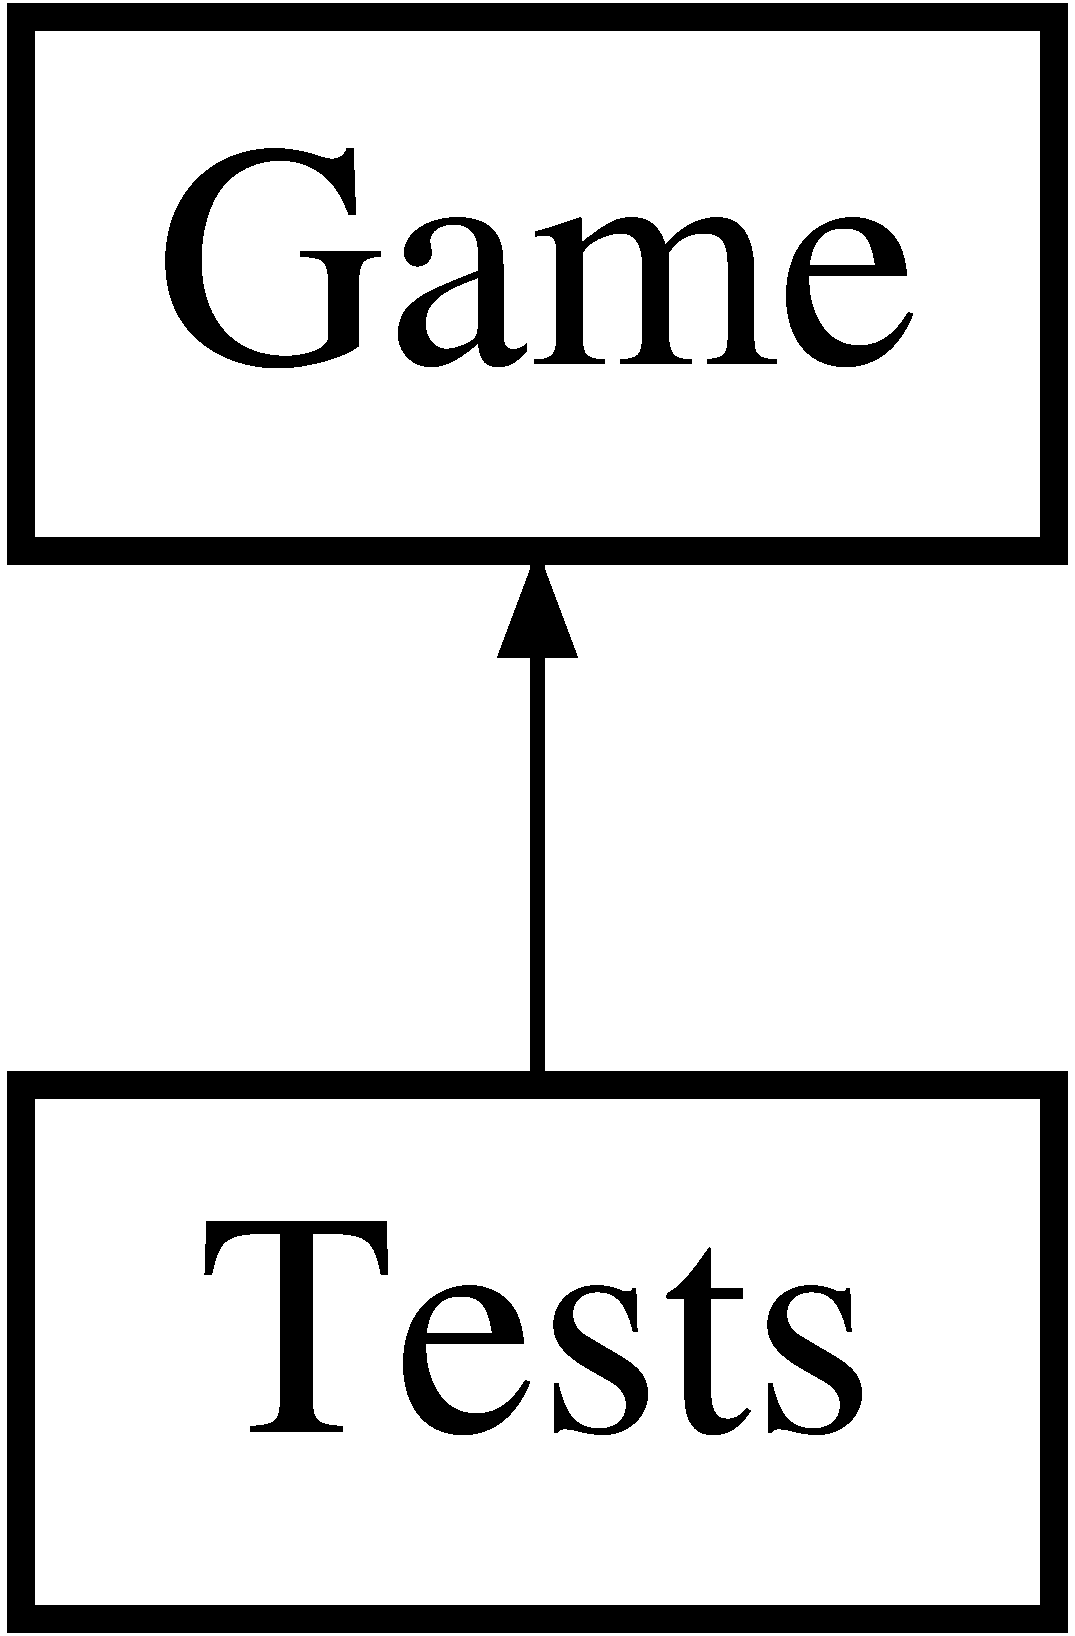
\includegraphics[height=2.000000cm]{classTests}
\end{center}
\end{figure}
\subsection*{Public Member Functions}
\begin{DoxyCompactItemize}
\item 
\hypertarget{classTests_a4ddcbb89a01d7e5317a03704cd077df2}{void {\bfseries game1} ()}\label{classTests_a4ddcbb89a01d7e5317a03704cd077df2}

\item 
\hypertarget{classTests_adcb4104bf3e71a817c65443a0e095cc7}{void {\bfseries game2} ()}\label{classTests_adcb4104bf3e71a817c65443a0e095cc7}

\item 
\hypertarget{classTests_a03c52a5d68e9aaf3d032e624041160c8}{void {\bfseries jagged\+Line} ()}\label{classTests_a03c52a5d68e9aaf3d032e624041160c8}

\item 
\hypertarget{classTests_a22394551fa9d1cc0707cc7b942a3714b}{void {\bfseries game1\+\_\+do\+Move} ()}\label{classTests_a22394551fa9d1cc0707cc7b942a3714b}

\item 
\hypertarget{classTests_a6b437e7b6b8c3d5f9865749eea129322}{void {\bfseries invalid\+Corner} ()}\label{classTests_a6b437e7b6b8c3d5f9865749eea129322}

\item 
\hypertarget{classTests_a624037459dcd5be353f290388337546a}{void {\bfseries invalid\+Line} ()}\label{classTests_a624037459dcd5be353f290388337546a}

\item 
\hypertarget{classTests_ada9fec53e6ed86ab994318ad5f91b94e}{void {\bfseries image\+Not\+Loaded} ()}\label{classTests_ada9fec53e6ed86ab994318ad5f91b94e}

\item 
\hypertarget{classTests_a280dd55f9ea89dc1aefff4a37c9ce418}{void {\bfseries copy\+Initialize} ()}\label{classTests_a280dd55f9ea89dc1aefff4a37c9ce418}

\item 
\hypertarget{classTests_aba00d7d16cba53fab489f9788e2bcc1f}{bool {\bfseries validate\+Copy} () const }\label{classTests_aba00d7d16cba53fab489f9788e2bcc1f}

\item 
\hypertarget{classTests_a0bbd4987e015b1f042a2e0f1eeb12d88}{void {\bfseries sdl\+Render\+Game} () const }\label{classTests_a0bbd4987e015b1f042a2e0f1eeb12d88}

\end{DoxyCompactItemize}
\subsection*{Additional Inherited Members}


\subsection{Detailed Description}


Definition at line 14 of file tests.\+h.



The documentation for this class was generated from the following files\+:\begin{DoxyCompactItemize}
\item 
tests/tests.\+h\item 
tests/exceptions.\+cpp\item 
tests/game1.\+cpp\item 
tests/game2.\+cpp\item 
tests/jagged.\+cpp\item 
tests/sdl\+Render.\+cpp\end{DoxyCompactItemize}

\hypertarget{structText_1_1TextProperties}{\section{Text\+:\+:Text\+Properties Struct Reference}
\label{structText_1_1TextProperties}\index{Text\+::\+Text\+Properties@{Text\+::\+Text\+Properties}}
}


Write what the function does here.  




{\ttfamily \#include $<$text.\+h$>$}

\subsection*{Public Attributes}
\begin{DoxyCompactItemize}
\item 
\hypertarget{structText_1_1TextProperties_a44233dc1053dea188f86428a2768b46c}{float {\bfseries tab\+Width} = 8}\label{structText_1_1TextProperties_a44233dc1053dea188f86428a2768b46c}

\end{DoxyCompactItemize}


\subsection{Detailed Description}
Write what the function does here. 


\begin{DoxyRetVals}{Return values}
{\em (variable)} & (description of variable) \\
\hline
\end{DoxyRetVals}


Definition at line 21 of file text.\+h.



The documentation for this struct was generated from the following file\+:\begin{DoxyCompactItemize}
\item 
text.\+h\end{DoxyCompactItemize}

\hypertarget{classTextureAtlas}{\section{Texture\+Atlas Class Reference}
\label{classTextureAtlas}\index{Texture\+Atlas@{Texture\+Atlas}}
}


Write what the function does here.  




{\ttfamily \#include $<$texture\+\_\+atlas.\+h$>$}

\subsection*{Public Types}
\begin{DoxyCompactItemize}
\item 
\hypertarget{classTextureAtlas_abbfdf3f234b54498fc3a107eddb6febe}{enum \{ {\bfseries texture\+X\+Res} = 256, 
{\bfseries texture\+Y\+Res} = 256
 \}}\label{classTextureAtlas_abbfdf3f234b54498fc3a107eddb6febe}

\end{DoxyCompactItemize}
\subsection*{Public Member Functions}
\begin{DoxyCompactItemize}
\item 
\hyperlink{classTextureAtlas_a5a0ce2e5d8c48be86fa8a1545610b523}{Texture\+Atlas} (int left, int top, int width, int height)
\begin{DoxyCompactList}\small\item\em Write what the function does here. \end{DoxyCompactList}\item 
\hypertarget{classTextureAtlas_a8c6ecca37b0bf2f2eb490a1cf209dffe}{const \hyperlink{classTextureAtlas}{Texture\+Atlas} \& {\bfseries operator=} (const \hyperlink{classTextureAtlas}{Texture\+Atlas} \&)=delete}\label{classTextureAtlas_a8c6ecca37b0bf2f2eb490a1cf209dffe}

\item 
\hyperlink{structTextureDescriptor}{Texture\+Descriptor} \hyperlink{classTextureAtlas_a30d1c868e881cb9254dad8fb107a8710}{td} () const 
\begin{DoxyCompactList}\small\item\em Write what the function does here. \end{DoxyCompactList}\item 
\hyperlink{structTextureDescriptor}{Texture\+Descriptor} \hyperlink{classTextureAtlas_aad55bc78b471d40ebe02e818f25e9da3}{td\+No\+Offset} () const 
\begin{DoxyCompactList}\small\item\em Write what the function does here. \end{DoxyCompactList}\end{DoxyCompactItemize}
\subsection*{Public Attributes}
\begin{DoxyCompactItemize}
\item 
\hypertarget{classTextureAtlas_a66451f0890d33e943f26b3d0ff073864}{const int {\bfseries left}}\label{classTextureAtlas_a66451f0890d33e943f26b3d0ff073864}

\item 
\hypertarget{classTextureAtlas_a75d33d1023c7a1d5bd9da3891018c8d4}{const int {\bfseries top}}\label{classTextureAtlas_a75d33d1023c7a1d5bd9da3891018c8d4}

\item 
\hypertarget{classTextureAtlas_a0bdebb01fa7731fb98420c024b6677e1}{const int {\bfseries width}}\label{classTextureAtlas_a0bdebb01fa7731fb98420c024b6677e1}

\item 
\hypertarget{classTextureAtlas_ab8a68953dfb57a24747bb4ec07a71d37}{const int {\bfseries height}}\label{classTextureAtlas_ab8a68953dfb57a24747bb4ec07a71d37}

\item 
const float \hyperlink{classTextureAtlas_a668da55e54ffc6ae084e3b67d39e1094}{min\+U}
\begin{DoxyCompactList}\small\item\em Write what the function does here. \end{DoxyCompactList}\item 
\hypertarget{classTextureAtlas_ab13e70b95c181acb72bbdbf89bb6126d}{const float {\bfseries max\+U}}\label{classTextureAtlas_ab13e70b95c181acb72bbdbf89bb6126d}

\item 
\hypertarget{classTextureAtlas_a55144ed06907322e6db2678d3cdf1911}{const float {\bfseries min\+V}}\label{classTextureAtlas_a55144ed06907322e6db2678d3cdf1911}

\item 
\hypertarget{classTextureAtlas_a0ca44f00d7d0a644a92a386d4db80504}{const float {\bfseries max\+V}}\label{classTextureAtlas_a0ca44f00d7d0a644a92a386d4db80504}

\end{DoxyCompactItemize}
\subsection*{Static Public Attributes}
\begin{DoxyCompactItemize}
\item 
\hypertarget{classTextureAtlas_a0980d47e7d18e1e22e3c8a6df22a0f01}{static const \hyperlink{classImage}{Image} {\bfseries texture} = load\+Image()}\label{classTextureAtlas_a0980d47e7d18e1e22e3c8a6df22a0f01}

\item 
\hypertarget{classTextureAtlas_af2e14712c23efb5aaa1c38b11af6d847}{static constexpr float {\bfseries pixel\+Offset} = 0.\+05f}\label{classTextureAtlas_af2e14712c23efb5aaa1c38b11af6d847}

\item 
\hypertarget{classTextureAtlas_a0cf72eb78cbcfea76a9651dfe7ee0c88}{static const \hyperlink{classTextureAtlas}{Texture\+Atlas} {\bfseries Font8x8}}\label{classTextureAtlas_a0cf72eb78cbcfea76a9651dfe7ee0c88}

\item 
\hypertarget{classTextureAtlas_a4296dc62e2df77b079d742514d730322}{static const \hyperlink{classTextureAtlas}{Texture\+Atlas} {\bfseries Line}}\label{classTextureAtlas_a4296dc62e2df77b079d742514d730322}

\item 
\hypertarget{classTextureAtlas_a8d23d56a964289978500e69b2f5da9d7}{static const \hyperlink{classTextureAtlas}{Texture\+Atlas} {\bfseries Point}}\label{classTextureAtlas_a8d23d56a964289978500e69b2f5da9d7}

\item 
\hypertarget{classTextureAtlas_a5de4d8256c307baf190b716165b55676}{static const \hyperlink{classTextureAtlas}{Texture\+Atlas} {\bfseries Button\+Left\+Diffuse}}\label{classTextureAtlas_a5de4d8256c307baf190b716165b55676}

\item 
\hypertarget{classTextureAtlas_a2ac1de24e854660b7719778fb2c34b05}{static const \hyperlink{classTextureAtlas}{Texture\+Atlas} {\bfseries Button\+Right\+Diffuse}}\label{classTextureAtlas_a2ac1de24e854660b7719778fb2c34b05}

\item 
\hypertarget{classTextureAtlas_a3cd755976a35facb8f1902227521d67e}{static const \hyperlink{classTextureAtlas}{Texture\+Atlas} {\bfseries Button\+Middle\+Diffuse}}\label{classTextureAtlas_a3cd755976a35facb8f1902227521d67e}

\item 
\hypertarget{classTextureAtlas_a43bdce582ca4245f963415cbce11de63}{static const \hyperlink{classTextureAtlas}{Texture\+Atlas} {\bfseries Button\+Left\+Specular}}\label{classTextureAtlas_a43bdce582ca4245f963415cbce11de63}

\item 
\hypertarget{classTextureAtlas_aba9ac7217c6089808af6739280ec7779}{static const \hyperlink{classTextureAtlas}{Texture\+Atlas} {\bfseries Button\+Right\+Specular}}\label{classTextureAtlas_aba9ac7217c6089808af6739280ec7779}

\item 
\hypertarget{classTextureAtlas_acc26c58bb000ae76c00d1ea32c98dc15}{static const \hyperlink{classTextureAtlas}{Texture\+Atlas} {\bfseries Button\+Middle\+Specular}}\label{classTextureAtlas_acc26c58bb000ae76c00d1ea32c98dc15}

\item 
\hypertarget{classTextureAtlas_a5cd1596a9c97776e0c1f417567700668}{static const \hyperlink{classTextureAtlas}{Texture\+Atlas} {\bfseries Menu\+Gear\+Top}}\label{classTextureAtlas_a5cd1596a9c97776e0c1f417567700668}

\item 
\hypertarget{classTextureAtlas_a94b67c9b1a5f697574cc17b269575db7}{static const \hyperlink{classTextureAtlas}{Texture\+Atlas} {\bfseries Menu\+Gear\+Bottom}}\label{classTextureAtlas_a94b67c9b1a5f697574cc17b269575db7}

\end{DoxyCompactItemize}


\subsection{Detailed Description}
Write what the function does here. 


\begin{DoxyRetVals}{Return values}
{\em (variable)} & (description of variable) \\
\hline
\end{DoxyRetVals}


Definition at line 10 of file texture\+\_\+atlas.\+h.



\subsection{Constructor \& Destructor Documentation}
\hypertarget{classTextureAtlas_a5a0ce2e5d8c48be86fa8a1545610b523}{\index{Texture\+Atlas@{Texture\+Atlas}!Texture\+Atlas@{Texture\+Atlas}}
\index{Texture\+Atlas@{Texture\+Atlas}!Texture\+Atlas@{Texture\+Atlas}}
\subsubsection[{Texture\+Atlas}]{\setlength{\rightskip}{0pt plus 5cm}Texture\+Atlas\+::\+Texture\+Atlas (
\begin{DoxyParamCaption}
\item[{int}]{left, }
\item[{int}]{top, }
\item[{int}]{width, }
\item[{int}]{height}
\end{DoxyParamCaption}
)\hspace{0.3cm}{\ttfamily [inline]}, {\ttfamily [explicit]}}}\label{classTextureAtlas_a5a0ce2e5d8c48be86fa8a1545610b523}


Write what the function does here. 


\begin{DoxyParams}{Parameters}
{\em pixel\+Offset} & \\
\hline
{\em texture\+Y\+Res} & \\
\hline
\end{DoxyParams}

\begin{DoxyRetVals}{Return values}
{\em (variable)} & (description of variable) \\
\hline
\end{DoxyRetVals}


Definition at line 28 of file texture\+\_\+atlas.\+h.


\begin{DoxyCode}
29             : left(left), top(top), width(width), height(height),
30             \hyperlink{classTextureAtlas_a668da55e54ffc6ae084e3b67d39e1094}{minU}((left + pixelOffset) / textureXRes),
31             maxU((left + width - pixelOffset) / textureXRes),
32             minV(1 - (top + height - pixelOffset) / textureYRes),
33 \textcolor{comment}{}
34 \textcolor{comment}{            /**}
35 \textcolor{comment}{             * @brief Write what the function does here}
36 \textcolor{comment}{             *}
37 \textcolor{comment}{             * @param pixelOffset}
38 \textcolor{comment}{             * @param textureYRes}
39 \textcolor{comment}{             *}
40 \textcolor{comment}{             * @retval (variable) (description of variable)}
41 \textcolor{comment}{             **/}
42             maxV(1 - (top + pixelOffset) / textureYRes)
43             \{
44             \}
\end{DoxyCode}


\subsection{Member Function Documentation}
\hypertarget{classTextureAtlas_a30d1c868e881cb9254dad8fb107a8710}{\index{Texture\+Atlas@{Texture\+Atlas}!td@{td}}
\index{td@{td}!Texture\+Atlas@{Texture\+Atlas}}
\subsubsection[{td}]{\setlength{\rightskip}{0pt plus 5cm}{\bf Texture\+Descriptor} Texture\+Atlas\+::td (
\begin{DoxyParamCaption}
{}
\end{DoxyParamCaption}
) const\hspace{0.3cm}{\ttfamily [inline]}}}\label{classTextureAtlas_a30d1c868e881cb9254dad8fb107a8710}


Write what the function does here. 


\begin{DoxyRetVals}{Return values}
{\em (variable)} & (description of variable) \\
\hline
\end{DoxyRetVals}


Definition at line 52 of file texture\+\_\+atlas.\+h.



References min\+U.


\begin{DoxyCode}
53         \{
54             \textcolor{keywordflow}{return} \hyperlink{structTextureDescriptor}{TextureDescriptor}(texture, \hyperlink{classTextureAtlas_a668da55e54ffc6ae084e3b67d39e1094}{minU}, maxU, minV, maxV);
55         \}
\end{DoxyCode}
\hypertarget{classTextureAtlas_aad55bc78b471d40ebe02e818f25e9da3}{\index{Texture\+Atlas@{Texture\+Atlas}!td\+No\+Offset@{td\+No\+Offset}}
\index{td\+No\+Offset@{td\+No\+Offset}!Texture\+Atlas@{Texture\+Atlas}}
\subsubsection[{td\+No\+Offset}]{\setlength{\rightskip}{0pt plus 5cm}{\bf Texture\+Descriptor} Texture\+Atlas\+::td\+No\+Offset (
\begin{DoxyParamCaption}
{}
\end{DoxyParamCaption}
) const\hspace{0.3cm}{\ttfamily [inline]}}}\label{classTextureAtlas_aad55bc78b471d40ebe02e818f25e9da3}


Write what the function does here. 


\begin{DoxyRetVals}{Return values}
{\em (variable)} & (description of variable) \\
\hline
\end{DoxyRetVals}


Definition at line 62 of file texture\+\_\+atlas.\+h.


\begin{DoxyCode}
63         \{
64             \textcolor{keywordflow}{return} \hyperlink{structTextureDescriptor}{TextureDescriptor}(texture, (\textcolor{keywordtype}{float})left / textureXRes, (\textcolor{keywordtype}{float})(left + 
      width) / textureXRes, 1 - (\textcolor{keywordtype}{float})(top + height) / textureYRes, 1 - (\textcolor{keywordtype}{float})top / textureYRes);
65         \}
\end{DoxyCode}


\subsection{Member Data Documentation}
\hypertarget{classTextureAtlas_a668da55e54ffc6ae084e3b67d39e1094}{\index{Texture\+Atlas@{Texture\+Atlas}!min\+U@{min\+U}}
\index{min\+U@{min\+U}!Texture\+Atlas@{Texture\+Atlas}}
\subsubsection[{min\+U}]{\setlength{\rightskip}{0pt plus 5cm}const float Texture\+Atlas\+::min\+U}}\label{classTextureAtlas_a668da55e54ffc6ae084e3b67d39e1094}


Write what the function does here. 


\begin{DoxyParams}{Parameters}
{\em min\+U} & \\
\hline
{\em max\+U} & \\
\hline
{\em min\+V} & \\
\hline
\end{DoxyParams}

\begin{DoxyRetVals}{Return values}
{\em (variable)} & (description of variable) \\
\hline
\end{DoxyRetVals}


Definition at line 25 of file texture\+\_\+atlas.\+h.



Referenced by td().



The documentation for this class was generated from the following files\+:\begin{DoxyCompactItemize}
\item 
texture\+\_\+atlas.\+h\item 
texture\+\_\+atlas.\+cpp\end{DoxyCompactItemize}

\hypertarget{structTextureCoord}{\section{Texture\+Coord Struct Reference}
\label{structTextureCoord}\index{Texture\+Coord@{Texture\+Coord}}
}


Write what the function does here.  




{\ttfamily \#include $<$mesh.\+h$>$}

\subsection*{Public Member Functions}
\begin{DoxyCompactItemize}
\item 
\hypertarget{structTextureCoord_a244f496ea94cf6a50be632a3ef7d36d2}{{\bfseries Texture\+Coord} (float u, float v)}\label{structTextureCoord_a244f496ea94cf6a50be632a3ef7d36d2}

\end{DoxyCompactItemize}
\subsection*{Public Attributes}
\begin{DoxyCompactItemize}
\item 
\hypertarget{structTextureCoord_ae64022a50d7a8c1522f1f07631135804}{float {\bfseries u}}\label{structTextureCoord_ae64022a50d7a8c1522f1f07631135804}

\item 
\hypertarget{structTextureCoord_af26c9cf30246ac6451d981bb836ae4b1}{float {\bfseries v}}\label{structTextureCoord_af26c9cf30246ac6451d981bb836ae4b1}

\end{DoxyCompactItemize}
\subsection*{Friends}
\begin{DoxyCompactItemize}
\item 
ostream \& \hyperlink{structTextureCoord_a30143be17ec2f3bbe4df4424e4ac8fb6}{operator$<$$<$} (ostream \&os, const \hyperlink{structTextureCoord}{Texture\+Coord} \&t)
\begin{DoxyCompactList}\small\item\em Write what the function does here. \end{DoxyCompactList}\end{DoxyCompactItemize}


\subsection{Detailed Description}
Write what the function does here. 

\begin{DoxyReturn}{Returns}

\end{DoxyReturn}


Definition at line 20 of file mesh.\+h.



\subsection{Friends And Related Function Documentation}
\hypertarget{structTextureCoord_a30143be17ec2f3bbe4df4424e4ac8fb6}{\index{Texture\+Coord@{Texture\+Coord}!operator$<$$<$@{operator$<$$<$}}
\index{operator$<$$<$@{operator$<$$<$}!Texture\+Coord@{Texture\+Coord}}
\subsubsection[{operator$<$$<$}]{\setlength{\rightskip}{0pt plus 5cm}ostream\& operator$<$$<$ (
\begin{DoxyParamCaption}
\item[{ostream \&}]{os, }
\item[{const {\bf Texture\+Coord} \&}]{t}
\end{DoxyParamCaption}
)\hspace{0.3cm}{\ttfamily [friend]}}}\label{structTextureCoord_a30143be17ec2f3bbe4df4424e4ac8fb6}


Write what the function does here. 


\begin{DoxyParams}{Parameters}
{\em os} & \\
\hline
{\em t} & \\
\hline
\end{DoxyParams}
\begin{DoxyReturn}{Returns}

\end{DoxyReturn}


Definition at line 40 of file mesh.\+h.


\begin{DoxyCode}
41     \{
42         \textcolor{keywordflow}{return} os << \textcolor{stringliteral}{"<"} << t.u << \textcolor{stringliteral}{", "} << t.v << \textcolor{stringliteral}{">"};
43     \}
\end{DoxyCode}


The documentation for this struct was generated from the following file\+:\begin{DoxyCompactItemize}
\item 
mesh.\+h\end{DoxyCompactItemize}

\hypertarget{structTextureDescriptor}{\section{Texture\+Descriptor Struct Reference}
\label{structTextureDescriptor}\index{Texture\+Descriptor@{Texture\+Descriptor}}
}


Write what the function does here.  




{\ttfamily \#include $<$texture\+\_\+descriptor.\+h$>$}

\subsection*{Public Member Functions}
\begin{DoxyCompactItemize}
\item 
\hypertarget{structTextureDescriptor_a96245b9611b645eac88050ef4d70f2c2}{{\bfseries Texture\+Descriptor} (\hyperlink{classImage}{Image} image=\hyperlink{classImage}{Image}())}\label{structTextureDescriptor_a96245b9611b645eac88050ef4d70f2c2}

\item 
\hypertarget{structTextureDescriptor_affe5fe65a87405a17a428fe725dc78c3}{{\bfseries Texture\+Descriptor} (\hyperlink{classImage}{Image} image, float min\+U, float max\+U, float min\+V, float max\+V)}\label{structTextureDescriptor_affe5fe65a87405a17a428fe725dc78c3}

\item 
\hyperlink{structTextureDescriptor_a41a7fa119f03e28d9b3ae556fb6ff268}{operator bool} () const 
\begin{DoxyCompactList}\small\item\em Write what the function does here. \end{DoxyCompactList}\item 
bool \hyperlink{structTextureDescriptor_ad0465f550a605451e2c40a31a491c7b6}{operator!} () const 
\begin{DoxyCompactList}\small\item\em Write what the function does here. \end{DoxyCompactList}\item 
\hyperlink{structTextureDescriptor}{Texture\+Descriptor} \hyperlink{structTextureDescriptor_a03c94da9644d4992e51768aca4eb22ae}{sub\+Texture} (const float min\+U, const float max\+U, const float min\+V, const float max\+V) const 
\begin{DoxyCompactList}\small\item\em Write what the function does here. \end{DoxyCompactList}\end{DoxyCompactItemize}
\subsection*{Public Attributes}
\begin{DoxyCompactItemize}
\item 
\hypertarget{structTextureDescriptor_a0cafe348fe84771a83d29330224a99f7}{\hyperlink{classImage}{Image} {\bfseries image}}\label{structTextureDescriptor_a0cafe348fe84771a83d29330224a99f7}

\item 
\hypertarget{structTextureDescriptor_a01a1eecc6d3a37e9dc47c4b660093e21}{float {\bfseries min\+U}}\label{structTextureDescriptor_a01a1eecc6d3a37e9dc47c4b660093e21}

\item 
\hypertarget{structTextureDescriptor_a9409e0cf7f7a82116311e53223587a40}{float {\bfseries max\+U}}\label{structTextureDescriptor_a9409e0cf7f7a82116311e53223587a40}

\item 
\hypertarget{structTextureDescriptor_a8cd78b8d1bbb63ada5b71af81b7faf6a}{float {\bfseries min\+V}}\label{structTextureDescriptor_a8cd78b8d1bbb63ada5b71af81b7faf6a}

\item 
\hypertarget{structTextureDescriptor_abd34635c386508ecca180818b20bfb78}{float {\bfseries max\+V}}\label{structTextureDescriptor_abd34635c386508ecca180818b20bfb78}

\end{DoxyCompactItemize}


\subsection{Detailed Description}
Write what the function does here. 


\begin{DoxyRetVals}{Return values}
{\em (variable)} & (description of variable) \\
\hline
\end{DoxyRetVals}


Definition at line 11 of file texture\+\_\+descriptor.\+h.



\subsection{Member Function Documentation}
\hypertarget{structTextureDescriptor_a41a7fa119f03e28d9b3ae556fb6ff268}{\index{Texture\+Descriptor@{Texture\+Descriptor}!operator bool@{operator bool}}
\index{operator bool@{operator bool}!Texture\+Descriptor@{Texture\+Descriptor}}
\subsubsection[{operator bool}]{\setlength{\rightskip}{0pt plus 5cm}Texture\+Descriptor\+::operator bool (
\begin{DoxyParamCaption}
{}
\end{DoxyParamCaption}
) const\hspace{0.3cm}{\ttfamily [inline]}}}\label{structTextureDescriptor_a41a7fa119f03e28d9b3ae556fb6ff268}


Write what the function does here. 


\begin{DoxyRetVals}{Return values}
{\em (variable)} & (description of variable) \\
\hline
\end{DoxyRetVals}


Definition at line 29 of file texture\+\_\+descriptor.\+h.


\begin{DoxyCode}
30     \{
31         \textcolor{keywordflow}{return} (\textcolor{keywordtype}{bool})image;
32     \}
\end{DoxyCode}
\hypertarget{structTextureDescriptor_ad0465f550a605451e2c40a31a491c7b6}{\index{Texture\+Descriptor@{Texture\+Descriptor}!operator"!@{operator"!}}
\index{operator"!@{operator"!}!Texture\+Descriptor@{Texture\+Descriptor}}
\subsubsection[{operator"!}]{\setlength{\rightskip}{0pt plus 5cm}bool Texture\+Descriptor\+::operator! (
\begin{DoxyParamCaption}
{}
\end{DoxyParamCaption}
) const\hspace{0.3cm}{\ttfamily [inline]}}}\label{structTextureDescriptor_ad0465f550a605451e2c40a31a491c7b6}


Write what the function does here. 


\begin{DoxyRetVals}{Return values}
{\em (variable)} & (description of variable) \\
\hline
\end{DoxyRetVals}


Definition at line 39 of file texture\+\_\+descriptor.\+h.


\begin{DoxyCode}
40     \{
41         \textcolor{keywordflow}{return} !image;
42     \}
\end{DoxyCode}
\hypertarget{structTextureDescriptor_a03c94da9644d4992e51768aca4eb22ae}{\index{Texture\+Descriptor@{Texture\+Descriptor}!sub\+Texture@{sub\+Texture}}
\index{sub\+Texture@{sub\+Texture}!Texture\+Descriptor@{Texture\+Descriptor}}
\subsubsection[{sub\+Texture}]{\setlength{\rightskip}{0pt plus 5cm}{\bf Texture\+Descriptor} Texture\+Descriptor\+::sub\+Texture (
\begin{DoxyParamCaption}
\item[{const float}]{min\+U, }
\item[{const float}]{max\+U, }
\item[{const float}]{min\+V, }
\item[{const float}]{max\+V}
\end{DoxyParamCaption}
) const\hspace{0.3cm}{\ttfamily [inline]}}}\label{structTextureDescriptor_a03c94da9644d4992e51768aca4eb22ae}


Write what the function does here. 


\begin{DoxyParams}{Parameters}
{\em min\+U} & \\
\hline
{\em max\+U} & \\
\hline
{\em min\+V} & \\
\hline
{\em max\+V} & \\
\hline
\end{DoxyParams}

\begin{DoxyRetVals}{Return values}
{\em (variable)} & (description of variable) \\
\hline
\end{DoxyRetVals}


Definition at line 54 of file texture\+\_\+descriptor.\+h.


\begin{DoxyCode}
55     \{
56         \textcolor{keywordflow}{return} \hyperlink{structTextureDescriptor}{TextureDescriptor}(image,
57                 interpolate(minU, this->minU, this->maxU),
58                 interpolate(maxU, this->minU, this->maxU),
59                 interpolate(minV, this->minV, this->maxV),
60                 interpolate(maxV, this->minV, this->maxV));
61     \}
\end{DoxyCode}


The documentation for this struct was generated from the following file\+:\begin{DoxyCompactItemize}
\item 
texture\+\_\+descriptor.\+h\end{DoxyCompactItemize}

\hypertarget{structTransformedMesh}{\section{Transformed\+Mesh Struct Reference}
\label{structTransformedMesh}\index{Transformed\+Mesh@{Transformed\+Mesh}}
}


Write what the function does here.  




{\ttfamily \#include $<$mesh.\+h$>$}

\subsection*{Public Member Functions}
\begin{DoxyCompactItemize}
\item 
\hypertarget{structTransformedMesh_a845e75bfa1617afc8bc6e7e75429fe48}{{\bfseries Transformed\+Mesh} (Mesh mesh, \hyperlink{classMatrix}{Matrix} tform, \hyperlink{structColor}{Color} factor=\hyperlink{structColor}{Color}(1, 1, 1, 1))}\label{structTransformedMesh_a845e75bfa1617afc8bc6e7e75429fe48}

\item 
\hyperlink{structTransformedMesh_ab2294d4ace15f6fbcae200d09f5d6910}{operator Mesh} () const 
\begin{DoxyCompactList}\small\item\em Write what the function does here. \end{DoxyCompactList}\end{DoxyCompactItemize}
\subsection*{Public Attributes}
\begin{DoxyCompactItemize}
\item 
\hypertarget{structTransformedMesh_a94d242137b194041a3028e07317d0d8c}{Mesh {\bfseries mesh}}\label{structTransformedMesh_a94d242137b194041a3028e07317d0d8c}

\item 
\hypertarget{structTransformedMesh_a5a1639367ab17697e8245105d18088ad}{\hyperlink{classMatrix}{Matrix} {\bfseries tform}}\label{structTransformedMesh_a5a1639367ab17697e8245105d18088ad}

\item 
\hypertarget{structTransformedMesh_a4b9116e548cf96c33298b72ffb7a76c9}{\hyperlink{structColor}{Color} {\bfseries factor}}\label{structTransformedMesh_a4b9116e548cf96c33298b72ffb7a76c9}

\end{DoxyCompactItemize}


\subsection{Detailed Description}
Write what the function does here. 


\begin{DoxyRetVals}{Return values}
{\em (variable)} & (description of variable) \\
\hline
\end{DoxyRetVals}


Definition at line 143 of file mesh.\+h.



\subsection{Member Function Documentation}
\hypertarget{structTransformedMesh_ab2294d4ace15f6fbcae200d09f5d6910}{\index{Transformed\+Mesh@{Transformed\+Mesh}!operator Mesh@{operator Mesh}}
\index{operator Mesh@{operator Mesh}!Transformed\+Mesh@{Transformed\+Mesh}}
\subsubsection[{operator Mesh}]{\setlength{\rightskip}{0pt plus 5cm}$\ast$ Transformed\+Mesh\+::operator Mesh (
\begin{DoxyParamCaption}
{}
\end{DoxyParamCaption}
) const\hspace{0.3cm}{\ttfamily [inline]}}}\label{structTransformedMesh_ab2294d4ace15f6fbcae200d09f5d6910}


Write what the function does here. 


\begin{DoxyRetVals}{Return values}
{\em (variable)} & (description of variable) \\
\hline
\end{DoxyRetVals}


Definition at line 1029 of file mesh.\+h.


\begin{DoxyCode}
1030 \{
1031     \textcolor{keywordflow}{return} Mesh(\textcolor{keyword}{new} \hyperlink{classMesh__t}{Mesh\_t}(*\textcolor{keyword}{this}));
1032 \}
\end{DoxyCode}


The documentation for this struct was generated from the following file\+:\begin{DoxyCompactItemize}
\item 
mesh.\+h\end{DoxyCompactItemize}

\hypertarget{structTriangle}{\section{Triangle Struct Reference}
\label{structTriangle}\index{Triangle@{Triangle}}
}


Write what the function does here.  




{\ttfamily \#include $<$mesh.\+h$>$}

\subsection*{Public Member Functions}
\begin{DoxyCompactItemize}
\item 
\hyperlink{structTriangle_aaefe4ed500c07918d30c6f0e286332c5}{Triangle} ()
\begin{DoxyCompactList}\small\item\em Write what the function does here. \end{DoxyCompactList}\item 
\hyperlink{structTriangle_a9a52ea935ddd91cf0b939f494e4a6a81}{Triangle} (\hyperlink{structVectorF}{Vector\+F} p1, \hyperlink{structColor}{Color} c1, \hyperlink{structTextureCoord}{Texture\+Coord} t1, \hyperlink{structVectorF}{Vector\+F} p2, \hyperlink{structColor}{Color} c2, \hyperlink{structTextureCoord}{Texture\+Coord} t2, \hyperlink{structVectorF}{Vector\+F} p3, \hyperlink{structColor}{Color} c3, \hyperlink{structTextureCoord}{Texture\+Coord} t3)
\begin{DoxyCompactList}\small\item\em Write what the function does here. \end{DoxyCompactList}\item 
\hyperlink{structVectorF}{Vector\+F} \hyperlink{structTriangle_aba3ae2681927a25f27972819cbdc474d}{normal} () const 
\begin{DoxyCompactList}\small\item\em Write what the function does here. \end{DoxyCompactList}\end{DoxyCompactItemize}
\subsection*{Public Attributes}
\begin{DoxyCompactItemize}
\item 
\hypertarget{structTriangle_a6d2156f7d6944742550a2cfb6565dd62}{\hyperlink{structVectorF}{Vector\+F} {\bfseries p} \mbox{[}3\mbox{]}}\label{structTriangle_a6d2156f7d6944742550a2cfb6565dd62}

\item 
\hypertarget{structTriangle_ae58b397dee189c1feac2812e6651789b}{\hyperlink{structColor}{Color} {\bfseries c} \mbox{[}3\mbox{]}}\label{structTriangle_ae58b397dee189c1feac2812e6651789b}

\item 
\hypertarget{structTriangle_a1ba7666b37300d1f30b45f30bd427df8}{\hyperlink{structTextureCoord}{Texture\+Coord} {\bfseries t} \mbox{[}3\mbox{]}}\label{structTriangle_a1ba7666b37300d1f30b45f30bd427df8}

\end{DoxyCompactItemize}


\subsection{Detailed Description}
Write what the function does here. 

\begin{DoxyReturn}{Returns}

\end{DoxyReturn}


Definition at line 66 of file mesh.\+h.



\subsection{Constructor \& Destructor Documentation}
\hypertarget{structTriangle_aaefe4ed500c07918d30c6f0e286332c5}{\index{Triangle@{Triangle}!Triangle@{Triangle}}
\index{Triangle@{Triangle}!Triangle@{Triangle}}
\subsubsection[{Triangle}]{\setlength{\rightskip}{0pt plus 5cm}Triangle\+::\+Triangle (
\begin{DoxyParamCaption}
{}
\end{DoxyParamCaption}
)\hspace{0.3cm}{\ttfamily [inline]}}}\label{structTriangle_aaefe4ed500c07918d30c6f0e286332c5}


Write what the function does here. 

\begin{DoxyReturn}{Returns}

\end{DoxyReturn}


Definition at line 77 of file mesh.\+h.


\begin{DoxyCode}
78     \{
79     \}
\end{DoxyCode}
\hypertarget{structTriangle_a9a52ea935ddd91cf0b939f494e4a6a81}{\index{Triangle@{Triangle}!Triangle@{Triangle}}
\index{Triangle@{Triangle}!Triangle@{Triangle}}
\subsubsection[{Triangle}]{\setlength{\rightskip}{0pt plus 5cm}Triangle\+::\+Triangle (
\begin{DoxyParamCaption}
\item[{{\bf Vector\+F}}]{p1, }
\item[{{\bf Color}}]{c1, }
\item[{{\bf Texture\+Coord}}]{t1, }
\item[{{\bf Vector\+F}}]{p2, }
\item[{{\bf Color}}]{c2, }
\item[{{\bf Texture\+Coord}}]{t2, }
\item[{{\bf Vector\+F}}]{p3, }
\item[{{\bf Color}}]{c3, }
\item[{{\bf Texture\+Coord}}]{t3}
\end{DoxyParamCaption}
)\hspace{0.3cm}{\ttfamily [inline]}}}\label{structTriangle_a9a52ea935ddd91cf0b939f494e4a6a81}


Write what the function does here. 


\begin{DoxyParams}{Parameters}
{\em p1} & \\
\hline
{\em c1} & \\
\hline
{\em t1} & \\
\hline
{\em p2} & \\
\hline
{\em c2} & \\
\hline
{\em t2} & \\
\hline
{\em p3} & \\
\hline
{\em c3} & \\
\hline
{\em t3} & \\
\hline
\end{DoxyParams}
\begin{DoxyReturn}{Returns}

\end{DoxyReturn}


Definition at line 96 of file mesh.\+h.


\begin{DoxyCode}
97     \{
98         p[0] = p1;
99         c[0] = c1;
100         t[0] = t1;
101         p[1] = p2;
102         c[1] = c2;
103         t[1] = t2;
104         p[2] = p3;
105         c[2] = c3;
106         t[2] = t3;
107     \}
\end{DoxyCode}


\subsection{Member Function Documentation}
\hypertarget{structTriangle_aba3ae2681927a25f27972819cbdc474d}{\index{Triangle@{Triangle}!normal@{normal}}
\index{normal@{normal}!Triangle@{Triangle}}
\subsubsection[{normal}]{\setlength{\rightskip}{0pt plus 5cm}{\bf Vector\+F} Triangle\+::normal (
\begin{DoxyParamCaption}
{}
\end{DoxyParamCaption}
) const\hspace{0.3cm}{\ttfamily [inline]}}}\label{structTriangle_aba3ae2681927a25f27972819cbdc474d}


Write what the function does here. 

\begin{DoxyReturn}{Returns}

\end{DoxyReturn}


Definition at line 114 of file mesh.\+h.


\begin{DoxyCode}
115     \{
116         \textcolor{keywordflow}{return} normalize(cross(p[1] - p[0], p[2] - p[0]));
117     \}
\end{DoxyCode}


The documentation for this struct was generated from the following file\+:\begin{DoxyCompactItemize}
\item 
mesh.\+h\end{DoxyCompactItemize}

\hypertarget{structUint64}{\section{Uint64 Struct Reference}
\label{structUint64}\index{Uint64@{Uint64}}
}
\subsection*{Public Attributes}
\begin{DoxyCompactItemize}
\item 
\hypertarget{structUint64_aebe59cbeb37832b60d27071eca9fef3f}{Uint32 {\bfseries hi}}\label{structUint64_aebe59cbeb37832b60d27071eca9fef3f}

\item 
\hypertarget{structUint64_a110735976529c94010e0e1ff33bcb116}{Uint32 {\bfseries lo}}\label{structUint64_a110735976529c94010e0e1ff33bcb116}

\end{DoxyCompactItemize}


\subsection{Detailed Description}


Definition at line 112 of file S\+D\+L\+\_\+stdinc.\+h.



The documentation for this struct was generated from the following file\+:\begin{DoxyCompactItemize}
\item 
codeblocks/include/\+S\+D\+L/S\+D\+L\+\_\+stdinc.\+h\end{DoxyCompactItemize}

\hypertarget{classUTFDataFormatException}{\section{U\+T\+F\+Data\+Format\+Exception Class Reference}
\label{classUTFDataFormatException}\index{U\+T\+F\+Data\+Format\+Exception@{U\+T\+F\+Data\+Format\+Exception}}
}


Write what the function does here.  




{\ttfamily \#include $<$stream.\+h$>$}

Inheritance diagram for U\+T\+F\+Data\+Format\+Exception\+:\begin{figure}[H]
\begin{center}
\leavevmode
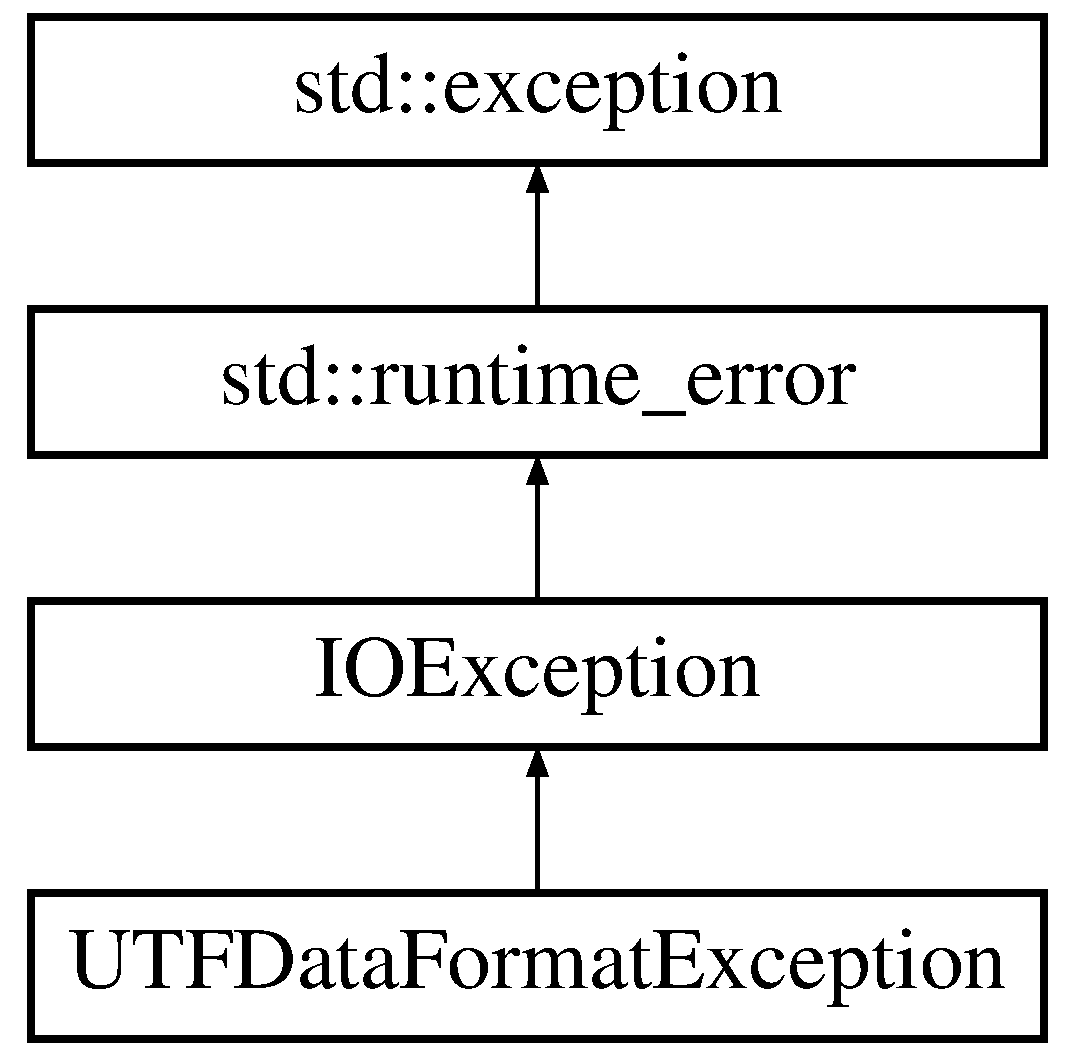
\includegraphics[height=4.000000cm]{classUTFDataFormatException}
\end{center}
\end{figure}
\subsection*{Additional Inherited Members}


\subsection{Detailed Description}
Write what the function does here. 

\begin{DoxyReturn}{Returns}

\end{DoxyReturn}


Definition at line 84 of file stream.\+h.



The documentation for this class was generated from the following file\+:\begin{DoxyCompactItemize}
\item 
stream.\+h\end{DoxyCompactItemize}

\hypertarget{structVectorF}{\section{Vector\+F Struct Reference}
\label{structVectorF}\index{Vector\+F@{Vector\+F}}
}


Write what the function does here.  




{\ttfamily \#include $<$vector.\+h$>$}

\subsection*{Public Member Functions}
\begin{DoxyCompactItemize}
\item 
constexpr \hyperlink{structVectorF_a0f4de0211dcec74e2cf31c3dbc8f6573}{Vector\+F} (float x, float y, float z)
\begin{DoxyCompactList}\small\item\em Write what the function does here. \end{DoxyCompactList}\item 
constexpr \hyperlink{structVectorF_a5bc6c2141ab8c3b26c3b15c3d2188e46}{Vector\+F} (float v=0)
\begin{DoxyCompactList}\small\item\em Write what the function does here. \end{DoxyCompactList}\item 
constexpr \hyperlink{structVectorF_aa06b752b0c00710c1d6d0c885686b282}{Vector\+F} (const \hyperlink{structVectorI}{Vector\+I} \&v)
\begin{DoxyCompactList}\small\item\em Write what the function does here. \end{DoxyCompactList}\item 
\hyperlink{structVectorF_a62bcc8b79ffdf1e6e1199d46ed800d78}{operator Vector\+I} () const 
\begin{DoxyCompactList}\small\item\em Write what the function does here. \end{DoxyCompactList}\item 
constexpr const \hyperlink{structVectorF}{Vector\+F} \hyperlink{structVectorF_a797fe54dd83c9a90bf538afdc60c8a31}{operator-\/} () const 
\begin{DoxyCompactList}\small\item\em Write what the function does here. \end{DoxyCompactList}\item 
constexpr const \hyperlink{structVectorF}{Vector\+F} \& \hyperlink{structVectorF_aad820d8b74b89970df0614f2dcfdf37c}{operator+} () const 
\begin{DoxyCompactList}\small\item\em Write what the function does here. \end{DoxyCompactList}\item 
constexpr const \hyperlink{structVectorF}{Vector\+F} \hyperlink{structVectorF_adb17836d5b5d7eeba62424c1d5f109e9}{operator+} (const \hyperlink{structVectorF}{Vector\+F} \&r) const 
\begin{DoxyCompactList}\small\item\em Write what the function does here. \end{DoxyCompactList}\item 
constexpr const \hyperlink{structVectorF}{Vector\+F} \hyperlink{structVectorF_aba20ab9c050dd441a9c3d0ec5fdde8ba}{operator-\/} (const \hyperlink{structVectorF}{Vector\+F} \&r) const 
\begin{DoxyCompactList}\small\item\em Write what the function does here. \end{DoxyCompactList}\item 
constexpr const \hyperlink{structVectorF}{Vector\+F} \hyperlink{structVectorF_a78cf7b725bb7724a8a3fb503baa129d7}{operator$\ast$} (const \hyperlink{structVectorF}{Vector\+F} \&r) const 
\begin{DoxyCompactList}\small\item\em Write what the function does here. \end{DoxyCompactList}\item 
constexpr const \hyperlink{structVectorF}{Vector\+F} \hyperlink{structVectorF_abb06f54310d9754e53d22e13073a706f}{operator/} (const \hyperlink{structVectorF}{Vector\+F} \&r) const 
\begin{DoxyCompactList}\small\item\em Write what the function does here. \end{DoxyCompactList}\item 
constexpr const \hyperlink{structVectorF}{Vector\+F} \hyperlink{structVectorF_a08f45eb79db6ea2dfdec066e366af752}{operator$\ast$} (float r) const 
\begin{DoxyCompactList}\small\item\em Write what the function does here. \end{DoxyCompactList}\item 
constexpr const \hyperlink{structVectorF}{Vector\+F} \hyperlink{structVectorF_a217a23d0ad4bcbe7d801d5df4399152f}{operator/} (float r) const 
\begin{DoxyCompactList}\small\item\em Write what the function does here. \end{DoxyCompactList}\item 
constexpr bool \hyperlink{structVectorF_a6ddfb24b4998b965c3f1348d6f15ee6f}{operator==} (const \hyperlink{structVectorF}{Vector\+F} \&r) const 
\begin{DoxyCompactList}\small\item\em Write what the function does here. \end{DoxyCompactList}\item 
constexpr bool \hyperlink{structVectorF_ae46d7475b96acfad53885c5b72621aa9}{operator!=} (const \hyperlink{structVectorF}{Vector\+F} \&r) const 
\begin{DoxyCompactList}\small\item\em Write what the function does here. \end{DoxyCompactList}\item 
const \hyperlink{structVectorF}{Vector\+F} \& \hyperlink{structVectorF_a767e52b421c36f5779d4eda65b965f4a}{operator+=} (const \hyperlink{structVectorF}{Vector\+F} \&r)
\begin{DoxyCompactList}\small\item\em Write what the function does here. \end{DoxyCompactList}\item 
const \hyperlink{structVectorF}{Vector\+F} \& \hyperlink{structVectorF_ad5ebdb98451cbc3d7c884cf3b89b963a}{operator-\/=} (const \hyperlink{structVectorF}{Vector\+F} \&r)
\begin{DoxyCompactList}\small\item\em Write what the function does here. \end{DoxyCompactList}\item 
const \hyperlink{structVectorF}{Vector\+F} \& \hyperlink{structVectorF_a88cf7042eb14233563d3019f2398bd32}{operator$\ast$=} (const \hyperlink{structVectorF}{Vector\+F} \&r)
\begin{DoxyCompactList}\small\item\em Write what the function does here. \end{DoxyCompactList}\item 
const \hyperlink{structVectorF}{Vector\+F} \& \hyperlink{structVectorF_af23ffd3fd18b6dde2eea6fdb17ad38af}{operator/=} (const \hyperlink{structVectorF}{Vector\+F} \&r)
\begin{DoxyCompactList}\small\item\em Write what the function does here. \end{DoxyCompactList}\item 
const \hyperlink{structVectorF}{Vector\+F} \& \hyperlink{structVectorF_a7eefa6afb0423e0d73b9f44a29941149}{operator$\ast$=} (float r)
\begin{DoxyCompactList}\small\item\em Write what the function does here. \end{DoxyCompactList}\item 
const \hyperlink{structVectorF}{Vector\+F} \& \hyperlink{structVectorF_ae7f9ffcce8e70e05d1f9608425e6a73c}{operator/=} (float r)
\begin{DoxyCompactList}\small\item\em Write what the function does here. \end{DoxyCompactList}\item 
float \hyperlink{structVectorF_a06ad6731ddd2591b29581f25eed20737}{phi} () const 
\begin{DoxyCompactList}\small\item\em Write what the function does here. \end{DoxyCompactList}\item 
float \hyperlink{structVectorF_a057b3c771f25463a76c1c9bc9425e663}{theta} () const 
\begin{DoxyCompactList}\small\item\em Write what the function does here. \end{DoxyCompactList}\item 
float \hyperlink{structVectorF_aabadea23e2330189a4fb35077c849b60}{r\+Spherical} () const 
\begin{DoxyCompactList}\small\item\em Write what the function does here. \end{DoxyCompactList}\end{DoxyCompactItemize}
\subsection*{Static Public Member Functions}
\begin{DoxyCompactItemize}
\item 
const static \hyperlink{structVectorF}{Vector\+F} \hyperlink{structVectorF_a553da195f30b0f0de5d856c80f7348ff}{normalize} (float x, float y, float z)
\begin{DoxyCompactList}\small\item\em Write what the function does here. \end{DoxyCompactList}\item 
{\footnotesize template$<$typename R\+E $>$ }\\static \hyperlink{structVectorF}{Vector\+F} \hyperlink{structVectorF_a4fa271c1382d384676561cc539b9abdb}{random} (R\+E \&re)
\begin{DoxyCompactList}\small\item\em Write what the function does here. \end{DoxyCompactList}\end{DoxyCompactItemize}
\subsection*{Public Attributes}
\begin{DoxyCompactItemize}
\item 
\hypertarget{structVectorF_ab7c47ac5d2e6cd5255e06fd70075a380}{float {\bfseries x}}\label{structVectorF_ab7c47ac5d2e6cd5255e06fd70075a380}

\item 
\hypertarget{structVectorF_a097b595dea00472dbbbdb507daef7495}{float {\bfseries y}}\label{structVectorF_a097b595dea00472dbbbdb507daef7495}

\item 
\hypertarget{structVectorF_a6e8e1e9a38b89c34fa378dc34b3ef915}{float {\bfseries z}}\label{structVectorF_a6e8e1e9a38b89c34fa378dc34b3ef915}

\end{DoxyCompactItemize}
\subsection*{Friends}
\begin{DoxyCompactItemize}
\item 
constexpr \hyperlink{structVectorF}{Vector\+F} \hyperlink{structVectorF_afa7c5f6c679bed0b801851befd794cb3}{operator+} (const \hyperlink{structVectorF}{Vector\+F} \&l, const \hyperlink{structVectorI}{Vector\+I} \&r)
\begin{DoxyCompactList}\small\item\em Write what the function does here. \end{DoxyCompactList}\item 
constexpr \hyperlink{structVectorF}{Vector\+F} \hyperlink{structVectorF_a1ce8a094648909e1206ed883059066eb}{operator+} (const \hyperlink{structVectorI}{Vector\+I} \&l, const \hyperlink{structVectorF}{Vector\+F} \&r)
\begin{DoxyCompactList}\small\item\em Write what the function does here. \end{DoxyCompactList}\item 
constexpr \hyperlink{structVectorF}{Vector\+F} \hyperlink{structVectorF_a8c841e23f2dce6697b7fb4df0d9112e8}{operator-\/} (const \hyperlink{structVectorF}{Vector\+F} \&l, const \hyperlink{structVectorI}{Vector\+I} \&r)
\begin{DoxyCompactList}\small\item\em Write what the function does here. \end{DoxyCompactList}\item 
constexpr \hyperlink{structVectorF}{Vector\+F} \hyperlink{structVectorF_aea94c6c9a31ed136700a8109b6bc3f00}{operator-\/} (const \hyperlink{structVectorI}{Vector\+I} \&l, const \hyperlink{structVectorF}{Vector\+F} \&r)
\begin{DoxyCompactList}\small\item\em Write what the function does here. \end{DoxyCompactList}\item 
constexpr \hyperlink{structVectorF}{Vector\+F} \hyperlink{structVectorF_a382c0752fd454c1cd3a1769a711fc092}{operator$\ast$} (const \hyperlink{structVectorF}{Vector\+F} \&l, const \hyperlink{structVectorI}{Vector\+I} \&r)
\begin{DoxyCompactList}\small\item\em Write what the function does here. \end{DoxyCompactList}\item 
constexpr \hyperlink{structVectorF}{Vector\+F} \hyperlink{structVectorF_add4f595c053e3ce987fa2086371af666}{operator$\ast$} (const \hyperlink{structVectorI}{Vector\+I} \&l, const \hyperlink{structVectorF}{Vector\+F} \&r)
\begin{DoxyCompactList}\small\item\em Write what the function does here. \end{DoxyCompactList}\item 
constexpr \hyperlink{structVectorF}{Vector\+F} \hyperlink{structVectorF_a95e18ed3b8a090fd040f5046a03682b9}{operator$\ast$} (float a, const \hyperlink{structVectorF}{Vector\+F} \&b)
\begin{DoxyCompactList}\small\item\em Write what the function does here. \end{DoxyCompactList}\item 
constexpr float \hyperlink{structVectorF_ae6a81a095a040050d82332d33b63b80d}{dot} (const \hyperlink{structVectorF}{Vector\+F} \&a, const \hyperlink{structVectorF}{Vector\+F} \&b)
\begin{DoxyCompactList}\small\item\em Write what the function does here. \end{DoxyCompactList}\item 
constexpr float \hyperlink{structVectorF_a5af45b716dd71b2e16c2c51cf451f4a9}{dot} (const \hyperlink{structVectorI}{Vector\+I} \&a, const \hyperlink{structVectorF}{Vector\+F} \&b)
\begin{DoxyCompactList}\small\item\em Write what the function does here. \end{DoxyCompactList}\item 
constexpr float \hyperlink{structVectorF_ac52ea832e6d54952f02b1d513e886993}{dot} (const \hyperlink{structVectorF}{Vector\+F} \&a, const \hyperlink{structVectorI}{Vector\+I} \&b)
\begin{DoxyCompactList}\small\item\em Write what the function does here. \end{DoxyCompactList}\item 
constexpr float \hyperlink{structVectorF_a1536c33d14bb5c290322c504e0f734b7}{abs\+Squared} (const \hyperlink{structVectorF}{Vector\+F} \&v)
\begin{DoxyCompactList}\small\item\em Write what the function does here. \end{DoxyCompactList}\item 
float \hyperlink{structVectorF_a34fe870a7141fd569c7144399f50c9a4}{abs} (const \hyperlink{structVectorF}{Vector\+F} \&v)
\begin{DoxyCompactList}\small\item\em Write what the function does here. \end{DoxyCompactList}\item 
const \hyperlink{structVectorF}{Vector\+F} \hyperlink{structVectorF_ac72c1e0aeaabb3f1b9749c409db9114a}{normalize\+No\+Throw} (const \hyperlink{structVectorF}{Vector\+F} \&v)
\begin{DoxyCompactList}\small\item\em Write what the function does here. \end{DoxyCompactList}\item 
const \hyperlink{structVectorF}{Vector\+F} \hyperlink{structVectorF_a97332544d415a8540da3caea6581c52d}{normalize} (const \hyperlink{structVectorF}{Vector\+F} v)
\begin{DoxyCompactList}\small\item\em Write what the function does here. \end{DoxyCompactList}\item 
constexpr \hyperlink{structVectorF}{Vector\+F} \hyperlink{structVectorF_a968c41313af492c22f946584e83fb9f5}{cross} (const \hyperlink{structVectorF}{Vector\+F} \&a, const \hyperlink{structVectorF}{Vector\+F} \&b)
\begin{DoxyCompactList}\small\item\em Write what the function does here. \end{DoxyCompactList}\item 
ostream \& \hyperlink{structVectorF_a2e9914517f8e728e8e4e735cc09e19a2}{operator$<$$<$} (ostream \&os, const \hyperlink{structVectorF}{Vector\+F} \&v)
\begin{DoxyCompactList}\small\item\em Write what the function does here. \end{DoxyCompactList}\end{DoxyCompactItemize}


\subsection{Detailed Description}
Write what the function does here. 

\begin{DoxyReturn}{Returns}

\end{DoxyReturn}


Definition at line 285 of file vector.\+h.



\subsection{Constructor \& Destructor Documentation}
\hypertarget{structVectorF_a0f4de0211dcec74e2cf31c3dbc8f6573}{\index{Vector\+F@{Vector\+F}!Vector\+F@{Vector\+F}}
\index{Vector\+F@{Vector\+F}!Vector\+F@{Vector\+F}}
\subsubsection[{Vector\+F}]{\setlength{\rightskip}{0pt plus 5cm}constexpr Vector\+F\+::\+Vector\+F (
\begin{DoxyParamCaption}
\item[{float}]{x, }
\item[{float}]{y, }
\item[{float}]{z}
\end{DoxyParamCaption}
)\hspace{0.3cm}{\ttfamily [inline]}}}\label{structVectorF_a0f4de0211dcec74e2cf31c3dbc8f6573}


Write what the function does here. 


\begin{DoxyParams}{Parameters}
{\em x} & \\
\hline
{\em y} & \\
\hline
{\em z} & \\
\hline
\end{DoxyParams}
\begin{DoxyReturn}{Returns}

\end{DoxyReturn}


Definition at line 288 of file vector.\+h.


\begin{DoxyCode}
299         : x(x), y(y), z(z)
300         \{
301         \}
\end{DoxyCode}
\hypertarget{structVectorF_a5bc6c2141ab8c3b26c3b15c3d2188e46}{\index{Vector\+F@{Vector\+F}!Vector\+F@{Vector\+F}}
\index{Vector\+F@{Vector\+F}!Vector\+F@{Vector\+F}}
\subsubsection[{Vector\+F}]{\setlength{\rightskip}{0pt plus 5cm}constexpr Vector\+F\+::\+Vector\+F (
\begin{DoxyParamCaption}
\item[{float}]{v = {\ttfamily 0}}
\end{DoxyParamCaption}
)\hspace{0.3cm}{\ttfamily [inline]}}}\label{structVectorF_a5bc6c2141ab8c3b26c3b15c3d2188e46}


Write what the function does here. 


\begin{DoxyParams}{Parameters}
{\em v} & \\
\hline
{\em v} & \\
\hline
{\em v} & \\
\hline
\end{DoxyParams}
\begin{DoxyReturn}{Returns}

\end{DoxyReturn}


Definition at line 302 of file vector.\+h.


\begin{DoxyCode}
313         : x(v), y(v), z(v)
314         \{
315         \}
\end{DoxyCode}
\hypertarget{structVectorF_aa06b752b0c00710c1d6d0c885686b282}{\index{Vector\+F@{Vector\+F}!Vector\+F@{Vector\+F}}
\index{Vector\+F@{Vector\+F}!Vector\+F@{Vector\+F}}
\subsubsection[{Vector\+F}]{\setlength{\rightskip}{0pt plus 5cm}constexpr Vector\+F\+::\+Vector\+F (
\begin{DoxyParamCaption}
\item[{const {\bf Vector\+I} \&}]{v}
\end{DoxyParamCaption}
)\hspace{0.3cm}{\ttfamily [inline]}}}\label{structVectorF_aa06b752b0c00710c1d6d0c885686b282}


Write what the function does here. 


\begin{DoxyParams}{Parameters}
{\em x} & \\
\hline
{\em y} & \\
\hline
{\em z} & \\
\hline
\end{DoxyParams}
\begin{DoxyReturn}{Returns}

\end{DoxyReturn}


Definition at line 316 of file vector.\+h.


\begin{DoxyCode}
327         : x(v.x), y(v.y), z(v.z)
328         \{
329         \}
\end{DoxyCode}


\subsection{Member Function Documentation}
\hypertarget{structVectorF_a553da195f30b0f0de5d856c80f7348ff}{\index{Vector\+F@{Vector\+F}!normalize@{normalize}}
\index{normalize@{normalize}!Vector\+F@{Vector\+F}}
\subsubsection[{normalize}]{\setlength{\rightskip}{0pt plus 5cm}const static {\bf Vector\+F} Vector\+F\+::normalize (
\begin{DoxyParamCaption}
\item[{float}]{x, }
\item[{float}]{y, }
\item[{float}]{z}
\end{DoxyParamCaption}
)\hspace{0.3cm}{\ttfamily [inline]}, {\ttfamily [static]}}}\label{structVectorF_a553da195f30b0f0de5d856c80f7348ff}


Write what the function does here. 


\begin{DoxyParams}{Parameters}
{\em x} & \\
\hline
{\em y} & \\
\hline
{\em z} & \\
\hline
\end{DoxyParams}
\begin{DoxyReturn}{Returns}

\end{DoxyReturn}
Write what the function does here


\begin{DoxyParams}{Parameters}
{\em 0} & \\
\hline
\end{DoxyParams}
\begin{DoxyReturn}{Returns}

\end{DoxyReturn}


Definition at line 760 of file vector.\+h.


\begin{DoxyCode}
761     \{
762         \hyperlink{structVectorF}{VectorF} v(x, y, z);
763         \textcolor{keywordtype}{float} r = \hyperlink{structVectorF_a34fe870a7141fd569c7144399f50c9a4}{abs}(v);
764 \textcolor{comment}{}
765 \textcolor{comment}{        /**}
766 \textcolor{comment}{         * @brief Write what the function does here}
767 \textcolor{comment}{         *}
768 \textcolor{comment}{         * @param 0}
769 \textcolor{comment}{         *}
770 \textcolor{comment}{         * @return}
771 \textcolor{comment}{         **/}
772         \textcolor{keywordflow}{if}(v == 0)
773         \{
774             \textcolor{keywordflow}{throw} domain\_error(\textcolor{stringliteral}{"can't normalize <0, 0, 0>"});
775         \}
776         \textcolor{keywordflow}{return} v / r;
777     \}
\end{DoxyCode}
\hypertarget{structVectorF_a62bcc8b79ffdf1e6e1199d46ed800d78}{\index{Vector\+F@{Vector\+F}!operator Vector\+I@{operator Vector\+I}}
\index{operator Vector\+I@{operator Vector\+I}!Vector\+F@{Vector\+F}}
\subsubsection[{operator Vector\+I}]{\setlength{\rightskip}{0pt plus 5cm}Vector\+F\+::operator {\bf Vector\+I} (
\begin{DoxyParamCaption}
{}
\end{DoxyParamCaption}
) const\hspace{0.3cm}{\ttfamily [inline]}, {\ttfamily [explicit]}}}\label{structVectorF_a62bcc8b79ffdf1e6e1199d46ed800d78}


Write what the function does here. 

\begin{DoxyReturn}{Returns}

\end{DoxyReturn}


Definition at line 336 of file vector.\+h.


\begin{DoxyCode}
337     \{
338         \textcolor{keywordflow}{return} \hyperlink{structVectorI}{VectorI}(ifloor(x), ifloor(y), ifloor(z));
339     \}
\end{DoxyCode}
\hypertarget{structVectorF_ae46d7475b96acfad53885c5b72621aa9}{\index{Vector\+F@{Vector\+F}!operator"!=@{operator"!=}}
\index{operator"!=@{operator"!=}!Vector\+F@{Vector\+F}}
\subsubsection[{operator"!=}]{\setlength{\rightskip}{0pt plus 5cm}constexpr bool Vector\+F\+::operator!= (
\begin{DoxyParamCaption}
\item[{const {\bf Vector\+F} \&}]{r}
\end{DoxyParamCaption}
) const\hspace{0.3cm}{\ttfamily [inline]}}}\label{structVectorF_ae46d7475b96acfad53885c5b72621aa9}


Write what the function does here. 


\begin{DoxyParams}{Parameters}
{\em r} & \\
\hline
\end{DoxyParams}
\begin{DoxyReturn}{Returns}

\end{DoxyReturn}


Definition at line 543 of file vector.\+h.


\begin{DoxyCode}
544     \{
545         \textcolor{keywordflow}{return} x != r.x || y != r.y || z != r.z;
546     \}
\end{DoxyCode}
\hypertarget{structVectorF_a78cf7b725bb7724a8a3fb503baa129d7}{\index{Vector\+F@{Vector\+F}!operator$\ast$@{operator$\ast$}}
\index{operator$\ast$@{operator$\ast$}!Vector\+F@{Vector\+F}}
\subsubsection[{operator$\ast$}]{\setlength{\rightskip}{0pt plus 5cm}constexpr const {\bf Vector\+F} Vector\+F\+::operator$\ast$ (
\begin{DoxyParamCaption}
\item[{const {\bf Vector\+F} \&}]{r}
\end{DoxyParamCaption}
) const\hspace{0.3cm}{\ttfamily [inline]}}}\label{structVectorF_a78cf7b725bb7724a8a3fb503baa129d7}


Write what the function does here. 


\begin{DoxyParams}{Parameters}
{\em r} & \\
\hline
\end{DoxyParams}
\begin{DoxyReturn}{Returns}

\end{DoxyReturn}


Definition at line 444 of file vector.\+h.


\begin{DoxyCode}
445     \{
446         \textcolor{keywordflow}{return} \hyperlink{structVectorF_a0f4de0211dcec74e2cf31c3dbc8f6573}{VectorF}(x * r.x, y * r.y, z * r.z);
447     \}
\end{DoxyCode}
\hypertarget{structVectorF_a08f45eb79db6ea2dfdec066e366af752}{\index{Vector\+F@{Vector\+F}!operator$\ast$@{operator$\ast$}}
\index{operator$\ast$@{operator$\ast$}!Vector\+F@{Vector\+F}}
\subsubsection[{operator$\ast$}]{\setlength{\rightskip}{0pt plus 5cm}constexpr const {\bf Vector\+F} Vector\+F\+::operator$\ast$ (
\begin{DoxyParamCaption}
\item[{float}]{r}
\end{DoxyParamCaption}
) const\hspace{0.3cm}{\ttfamily [inline]}}}\label{structVectorF_a08f45eb79db6ea2dfdec066e366af752}


Write what the function does here. 


\begin{DoxyParams}{Parameters}
{\em r} & \\
\hline
\end{DoxyParams}
\begin{DoxyReturn}{Returns}

\end{DoxyReturn}


Definition at line 494 of file vector.\+h.


\begin{DoxyCode}
495     \{
496         \textcolor{keywordflow}{return} \hyperlink{structVectorF_a0f4de0211dcec74e2cf31c3dbc8f6573}{VectorF}(x * r, y * r, z * r);
497     \}
\end{DoxyCode}
\hypertarget{structVectorF_a88cf7042eb14233563d3019f2398bd32}{\index{Vector\+F@{Vector\+F}!operator$\ast$=@{operator$\ast$=}}
\index{operator$\ast$=@{operator$\ast$=}!Vector\+F@{Vector\+F}}
\subsubsection[{operator$\ast$=}]{\setlength{\rightskip}{0pt plus 5cm}const {\bf Vector\+F}\& Vector\+F\+::operator$\ast$= (
\begin{DoxyParamCaption}
\item[{const {\bf Vector\+F} \&}]{r}
\end{DoxyParamCaption}
)\hspace{0.3cm}{\ttfamily [inline]}}}\label{structVectorF_a88cf7042eb14233563d3019f2398bd32}


Write what the function does here. 


\begin{DoxyParams}{Parameters}
{\em r} & \\
\hline
\end{DoxyParams}
\begin{DoxyReturn}{Returns}

\end{DoxyReturn}


Definition at line 585 of file vector.\+h.


\begin{DoxyCode}
586     \{
587         x *= r.x;
588         y *= r.y;
589         z *= r.z;
590         \textcolor{keywordflow}{return} *\textcolor{keyword}{this};
591     \}
\end{DoxyCode}
\hypertarget{structVectorF_a7eefa6afb0423e0d73b9f44a29941149}{\index{Vector\+F@{Vector\+F}!operator$\ast$=@{operator$\ast$=}}
\index{operator$\ast$=@{operator$\ast$=}!Vector\+F@{Vector\+F}}
\subsubsection[{operator$\ast$=}]{\setlength{\rightskip}{0pt plus 5cm}const {\bf Vector\+F}\& Vector\+F\+::operator$\ast$= (
\begin{DoxyParamCaption}
\item[{float}]{r}
\end{DoxyParamCaption}
)\hspace{0.3cm}{\ttfamily [inline]}}}\label{structVectorF_a7eefa6afb0423e0d73b9f44a29941149}


Write what the function does here. 


\begin{DoxyParams}{Parameters}
{\em r} & \\
\hline
\end{DoxyParams}
\begin{DoxyReturn}{Returns}

\end{DoxyReturn}


Definition at line 615 of file vector.\+h.


\begin{DoxyCode}
616     \{
617         x *= r;
618         y *= r;
619         z *= r;
620         \textcolor{keywordflow}{return} *\textcolor{keyword}{this};
621     \}
\end{DoxyCode}
\hypertarget{structVectorF_aad820d8b74b89970df0614f2dcfdf37c}{\index{Vector\+F@{Vector\+F}!operator+@{operator+}}
\index{operator+@{operator+}!Vector\+F@{Vector\+F}}
\subsubsection[{operator+}]{\setlength{\rightskip}{0pt plus 5cm}constexpr const {\bf Vector\+F}\& Vector\+F\+::operator+ (
\begin{DoxyParamCaption}
{}
\end{DoxyParamCaption}
) const\hspace{0.3cm}{\ttfamily [inline]}}}\label{structVectorF_aad820d8b74b89970df0614f2dcfdf37c}


Write what the function does here. 

\begin{DoxyReturn}{Returns}

\end{DoxyReturn}


Definition at line 356 of file vector.\+h.


\begin{DoxyCode}
357     \{
358         \textcolor{keywordflow}{return} *\textcolor{keyword}{this};
359     \}
\end{DoxyCode}
\hypertarget{structVectorF_adb17836d5b5d7eeba62424c1d5f109e9}{\index{Vector\+F@{Vector\+F}!operator+@{operator+}}
\index{operator+@{operator+}!Vector\+F@{Vector\+F}}
\subsubsection[{operator+}]{\setlength{\rightskip}{0pt plus 5cm}constexpr const {\bf Vector\+F} Vector\+F\+::operator+ (
\begin{DoxyParamCaption}
\item[{const {\bf Vector\+F} \&}]{r}
\end{DoxyParamCaption}
) const\hspace{0.3cm}{\ttfamily [inline]}}}\label{structVectorF_adb17836d5b5d7eeba62424c1d5f109e9}


Write what the function does here. 


\begin{DoxyParams}{Parameters}
{\em r} & \\
\hline
\end{DoxyParams}
\begin{DoxyReturn}{Returns}

\end{DoxyReturn}


Definition at line 368 of file vector.\+h.


\begin{DoxyCode}
369     \{
370         \textcolor{keywordflow}{return} \hyperlink{structVectorF_a0f4de0211dcec74e2cf31c3dbc8f6573}{VectorF}(x + r.x, y + r.y, z + r.z);
371     \}
\end{DoxyCode}
\hypertarget{structVectorF_a767e52b421c36f5779d4eda65b965f4a}{\index{Vector\+F@{Vector\+F}!operator+=@{operator+=}}
\index{operator+=@{operator+=}!Vector\+F@{Vector\+F}}
\subsubsection[{operator+=}]{\setlength{\rightskip}{0pt plus 5cm}const {\bf Vector\+F}\& Vector\+F\+::operator+= (
\begin{DoxyParamCaption}
\item[{const {\bf Vector\+F} \&}]{r}
\end{DoxyParamCaption}
)\hspace{0.3cm}{\ttfamily [inline]}}}\label{structVectorF_a767e52b421c36f5779d4eda65b965f4a}


Write what the function does here. 


\begin{DoxyParams}{Parameters}
{\em r} & \\
\hline
\end{DoxyParams}
\begin{DoxyReturn}{Returns}

\end{DoxyReturn}


Definition at line 555 of file vector.\+h.


\begin{DoxyCode}
556     \{
557         x += r.x;
558         y += r.y;
559         z += r.z;
560         \textcolor{keywordflow}{return} *\textcolor{keyword}{this};
561     \}
\end{DoxyCode}
\hypertarget{structVectorF_a797fe54dd83c9a90bf538afdc60c8a31}{\index{Vector\+F@{Vector\+F}!operator-\/@{operator-\/}}
\index{operator-\/@{operator-\/}!Vector\+F@{Vector\+F}}
\subsubsection[{operator-\/}]{\setlength{\rightskip}{0pt plus 5cm}constexpr const {\bf Vector\+F} Vector\+F\+::operator-\/ (
\begin{DoxyParamCaption}
{}
\end{DoxyParamCaption}
) const\hspace{0.3cm}{\ttfamily [inline]}}}\label{structVectorF_a797fe54dd83c9a90bf538afdc60c8a31}


Write what the function does here. 

\begin{DoxyReturn}{Returns}

\end{DoxyReturn}


Definition at line 346 of file vector.\+h.


\begin{DoxyCode}
347     \{
348         \textcolor{keywordflow}{return} \hyperlink{structVectorF_a0f4de0211dcec74e2cf31c3dbc8f6573}{VectorF}(-x, -y, -z);
349     \}
\end{DoxyCode}
\hypertarget{structVectorF_aba20ab9c050dd441a9c3d0ec5fdde8ba}{\index{Vector\+F@{Vector\+F}!operator-\/@{operator-\/}}
\index{operator-\/@{operator-\/}!Vector\+F@{Vector\+F}}
\subsubsection[{operator-\/}]{\setlength{\rightskip}{0pt plus 5cm}constexpr const {\bf Vector\+F} Vector\+F\+::operator-\/ (
\begin{DoxyParamCaption}
\item[{const {\bf Vector\+F} \&}]{r}
\end{DoxyParamCaption}
) const\hspace{0.3cm}{\ttfamily [inline]}}}\label{structVectorF_aba20ab9c050dd441a9c3d0ec5fdde8ba}


Write what the function does here. 


\begin{DoxyParams}{Parameters}
{\em r} & \\
\hline
\end{DoxyParams}
\begin{DoxyReturn}{Returns}

\end{DoxyReturn}


Definition at line 406 of file vector.\+h.


\begin{DoxyCode}
407     \{
408         \textcolor{keywordflow}{return} \hyperlink{structVectorF_a0f4de0211dcec74e2cf31c3dbc8f6573}{VectorF}(x - r.x, y - r.y, z - r.z);
409     \}
\end{DoxyCode}
\hypertarget{structVectorF_ad5ebdb98451cbc3d7c884cf3b89b963a}{\index{Vector\+F@{Vector\+F}!operator-\/=@{operator-\/=}}
\index{operator-\/=@{operator-\/=}!Vector\+F@{Vector\+F}}
\subsubsection[{operator-\/=}]{\setlength{\rightskip}{0pt plus 5cm}const {\bf Vector\+F}\& Vector\+F\+::operator-\/= (
\begin{DoxyParamCaption}
\item[{const {\bf Vector\+F} \&}]{r}
\end{DoxyParamCaption}
)\hspace{0.3cm}{\ttfamily [inline]}}}\label{structVectorF_ad5ebdb98451cbc3d7c884cf3b89b963a}


Write what the function does here. 


\begin{DoxyParams}{Parameters}
{\em r} & \\
\hline
\end{DoxyParams}
\begin{DoxyReturn}{Returns}

\end{DoxyReturn}


Definition at line 570 of file vector.\+h.


\begin{DoxyCode}
571     \{
572         x -= r.x;
573         y -= r.y;
574         z -= r.z;
575         \textcolor{keywordflow}{return} *\textcolor{keyword}{this};
576     \}
\end{DoxyCode}
\hypertarget{structVectorF_abb06f54310d9754e53d22e13073a706f}{\index{Vector\+F@{Vector\+F}!operator/@{operator/}}
\index{operator/@{operator/}!Vector\+F@{Vector\+F}}
\subsubsection[{operator/}]{\setlength{\rightskip}{0pt plus 5cm}constexpr const {\bf Vector\+F} Vector\+F\+::operator/ (
\begin{DoxyParamCaption}
\item[{const {\bf Vector\+F} \&}]{r}
\end{DoxyParamCaption}
) const\hspace{0.3cm}{\ttfamily [inline]}}}\label{structVectorF_abb06f54310d9754e53d22e13073a706f}


Write what the function does here. 


\begin{DoxyParams}{Parameters}
{\em r} & \\
\hline
\end{DoxyParams}
\begin{DoxyReturn}{Returns}

\end{DoxyReturn}


Definition at line 482 of file vector.\+h.


\begin{DoxyCode}
483     \{
484         \textcolor{keywordflow}{return} \hyperlink{structVectorF_a0f4de0211dcec74e2cf31c3dbc8f6573}{VectorF}(x / r.x, y / r.y, z / r.z);
485     \}
\end{DoxyCode}
\hypertarget{structVectorF_a217a23d0ad4bcbe7d801d5df4399152f}{\index{Vector\+F@{Vector\+F}!operator/@{operator/}}
\index{operator/@{operator/}!Vector\+F@{Vector\+F}}
\subsubsection[{operator/}]{\setlength{\rightskip}{0pt plus 5cm}constexpr const {\bf Vector\+F} Vector\+F\+::operator/ (
\begin{DoxyParamCaption}
\item[{float}]{r}
\end{DoxyParamCaption}
) const\hspace{0.3cm}{\ttfamily [inline]}}}\label{structVectorF_a217a23d0ad4bcbe7d801d5df4399152f}


Write what the function does here. 


\begin{DoxyParams}{Parameters}
{\em r} & \\
\hline
\end{DoxyParams}
\begin{DoxyReturn}{Returns}

\end{DoxyReturn}


Definition at line 519 of file vector.\+h.


\begin{DoxyCode}
520     \{
521         \textcolor{keywordflow}{return} \hyperlink{structVectorF_a0f4de0211dcec74e2cf31c3dbc8f6573}{VectorF}(x / r, y / r, z / r);
522     \}
\end{DoxyCode}
\hypertarget{structVectorF_af23ffd3fd18b6dde2eea6fdb17ad38af}{\index{Vector\+F@{Vector\+F}!operator/=@{operator/=}}
\index{operator/=@{operator/=}!Vector\+F@{Vector\+F}}
\subsubsection[{operator/=}]{\setlength{\rightskip}{0pt plus 5cm}const {\bf Vector\+F}\& Vector\+F\+::operator/= (
\begin{DoxyParamCaption}
\item[{const {\bf Vector\+F} \&}]{r}
\end{DoxyParamCaption}
)\hspace{0.3cm}{\ttfamily [inline]}}}\label{structVectorF_af23ffd3fd18b6dde2eea6fdb17ad38af}


Write what the function does here. 


\begin{DoxyParams}{Parameters}
{\em r} & \\
\hline
\end{DoxyParams}
\begin{DoxyReturn}{Returns}

\end{DoxyReturn}


Definition at line 600 of file vector.\+h.


\begin{DoxyCode}
601     \{
602         x /= r.x;
603         y /= r.y;
604         z /= r.z;
605         \textcolor{keywordflow}{return} *\textcolor{keyword}{this};
606     \}
\end{DoxyCode}
\hypertarget{structVectorF_ae7f9ffcce8e70e05d1f9608425e6a73c}{\index{Vector\+F@{Vector\+F}!operator/=@{operator/=}}
\index{operator/=@{operator/=}!Vector\+F@{Vector\+F}}
\subsubsection[{operator/=}]{\setlength{\rightskip}{0pt plus 5cm}const {\bf Vector\+F}\& Vector\+F\+::operator/= (
\begin{DoxyParamCaption}
\item[{float}]{r}
\end{DoxyParamCaption}
)\hspace{0.3cm}{\ttfamily [inline]}}}\label{structVectorF_ae7f9ffcce8e70e05d1f9608425e6a73c}


Write what the function does here. 


\begin{DoxyParams}{Parameters}
{\em r} & \\
\hline
\end{DoxyParams}
\begin{DoxyReturn}{Returns}

\end{DoxyReturn}


Definition at line 630 of file vector.\+h.


\begin{DoxyCode}
631     \{
632         x /= r;
633         y /= r;
634         z /= r;
635         \textcolor{keywordflow}{return} *\textcolor{keyword}{this};
636     \}
\end{DoxyCode}
\hypertarget{structVectorF_a6ddfb24b4998b965c3f1348d6f15ee6f}{\index{Vector\+F@{Vector\+F}!operator==@{operator==}}
\index{operator==@{operator==}!Vector\+F@{Vector\+F}}
\subsubsection[{operator==}]{\setlength{\rightskip}{0pt plus 5cm}constexpr bool Vector\+F\+::operator== (
\begin{DoxyParamCaption}
\item[{const {\bf Vector\+F} \&}]{r}
\end{DoxyParamCaption}
) const\hspace{0.3cm}{\ttfamily [inline]}}}\label{structVectorF_a6ddfb24b4998b965c3f1348d6f15ee6f}


Write what the function does here. 


\begin{DoxyParams}{Parameters}
{\em r} & \\
\hline
\end{DoxyParams}
\begin{DoxyReturn}{Returns}

\end{DoxyReturn}


Definition at line 531 of file vector.\+h.


\begin{DoxyCode}
532     \{
533         \textcolor{keywordflow}{return} x == r.x && y == r.y && z == r.z;
534     \}
\end{DoxyCode}
\hypertarget{structVectorF_a06ad6731ddd2591b29581f25eed20737}{\index{Vector\+F@{Vector\+F}!phi@{phi}}
\index{phi@{phi}!Vector\+F@{Vector\+F}}
\subsubsection[{phi}]{\setlength{\rightskip}{0pt plus 5cm}float Vector\+F\+::phi (
\begin{DoxyParamCaption}
{}
\end{DoxyParamCaption}
) const\hspace{0.3cm}{\ttfamily [inline]}}}\label{structVectorF_a06ad6731ddd2591b29581f25eed20737}


Write what the function does here. 

\begin{DoxyReturn}{Returns}

\end{DoxyReturn}
Write what the function does here


\begin{DoxyParams}{Parameters}
{\em 0} & \\
\hline
\end{DoxyParams}
\begin{DoxyReturn}{Returns}

\end{DoxyReturn}


Definition at line 784 of file vector.\+h.


\begin{DoxyCode}
785     \{
786         \textcolor{keywordtype}{float} r = \hyperlink{structVectorF_a34fe870a7141fd569c7144399f50c9a4}{abs}(*\textcolor{keyword}{this});
787 \textcolor{comment}{}
788 \textcolor{comment}{        /**}
789 \textcolor{comment}{         * @brief Write what the function does here}
790 \textcolor{comment}{         *}
791 \textcolor{comment}{         * @param 0}
792 \textcolor{comment}{         *}
793 \textcolor{comment}{         * @return}
794 \textcolor{comment}{         **/}
795         \textcolor{keywordflow}{if}(r == 0)
796         \{
797             \textcolor{keywordflow}{return} 0;
798         \}
799         \textcolor{keywordtype}{float} v = y / r;
800         v = limit(v, -1.0f, 1.0f);
801         \textcolor{keywordflow}{return} asin(v);
802     \}
\end{DoxyCode}
\hypertarget{structVectorF_a4fa271c1382d384676561cc539b9abdb}{\index{Vector\+F@{Vector\+F}!random@{random}}
\index{random@{random}!Vector\+F@{Vector\+F}}
\subsubsection[{random}]{\setlength{\rightskip}{0pt plus 5cm}template$<$typename R\+E $>$ static {\bf Vector\+F} Vector\+F\+::random (
\begin{DoxyParamCaption}
\item[{R\+E \&}]{re}
\end{DoxyParamCaption}
)\hspace{0.3cm}{\ttfamily [inline]}, {\ttfamily [static]}}}\label{structVectorF_a4fa271c1382d384676561cc539b9abdb}


Write what the function does here. 


\begin{DoxyParams}{Parameters}
{\em re} & \\
\hline
\end{DoxyParams}
\begin{DoxyReturn}{Returns}

\end{DoxyReturn}
Write what the function does here

\begin{DoxyReturn}{Returns}

\end{DoxyReturn}


Definition at line 845 of file vector.\+h.


\begin{DoxyCode}
846         \{
847             \hyperlink{structVectorF}{VectorF} retval;
848 \textcolor{comment}{}
849 \textcolor{comment}{            /**}
850 \textcolor{comment}{             * @brief Write what the function does here}
851 \textcolor{comment}{             *}
852 \textcolor{comment}{             * @return}
853 \textcolor{comment}{             **/}
854             \textcolor{keywordflow}{do}
855             \{
856                 retval.x = uniform\_real\_distribution<float>(-1, 1)(re);
857                 retval.y = uniform\_real\_distribution<float>(-1, 1)(re);
858                 retval.z = uniform\_real\_distribution<float>(-1, 1)(re);
859             \}
860             \textcolor{keywordflow}{while}(\hyperlink{structVectorF_a1536c33d14bb5c290322c504e0f734b7}{absSquared}(retval) > 1 || \hyperlink{structVectorF_a1536c33d14bb5c290322c504e0f734b7}{absSquared}(retval) < eps);
861             \textcolor{keywordflow}{return} retval;
862         \}
\end{DoxyCode}
\hypertarget{structVectorF_aabadea23e2330189a4fb35077c849b60}{\index{Vector\+F@{Vector\+F}!r\+Spherical@{r\+Spherical}}
\index{r\+Spherical@{r\+Spherical}!Vector\+F@{Vector\+F}}
\subsubsection[{r\+Spherical}]{\setlength{\rightskip}{0pt plus 5cm}float Vector\+F\+::r\+Spherical (
\begin{DoxyParamCaption}
{}
\end{DoxyParamCaption}
) const\hspace{0.3cm}{\ttfamily [inline]}}}\label{structVectorF_aabadea23e2330189a4fb35077c849b60}


Write what the function does here. 

\begin{DoxyReturn}{Returns}

\end{DoxyReturn}


Definition at line 819 of file vector.\+h.


\begin{DoxyCode}
820     \{
821         \textcolor{keywordflow}{return} \hyperlink{structVectorF_a34fe870a7141fd569c7144399f50c9a4}{abs}(*\textcolor{keyword}{this});
822     \}
\end{DoxyCode}
\hypertarget{structVectorF_a057b3c771f25463a76c1c9bc9425e663}{\index{Vector\+F@{Vector\+F}!theta@{theta}}
\index{theta@{theta}!Vector\+F@{Vector\+F}}
\subsubsection[{theta}]{\setlength{\rightskip}{0pt plus 5cm}float Vector\+F\+::theta (
\begin{DoxyParamCaption}
{}
\end{DoxyParamCaption}
) const\hspace{0.3cm}{\ttfamily [inline]}}}\label{structVectorF_a057b3c771f25463a76c1c9bc9425e663}


Write what the function does here. 

\begin{DoxyReturn}{Returns}

\end{DoxyReturn}


Definition at line 809 of file vector.\+h.


\begin{DoxyCode}
810     \{
811         \textcolor{keywordflow}{return} atan2(x, z);
812     \}
\end{DoxyCode}


\subsection{Friends And Related Function Documentation}
\hypertarget{structVectorF_a34fe870a7141fd569c7144399f50c9a4}{\index{Vector\+F@{Vector\+F}!abs@{abs}}
\index{abs@{abs}!Vector\+F@{Vector\+F}}
\subsubsection[{abs}]{\setlength{\rightskip}{0pt plus 5cm}float abs (
\begin{DoxyParamCaption}
\item[{const {\bf Vector\+F} \&}]{v}
\end{DoxyParamCaption}
)\hspace{0.3cm}{\ttfamily [friend]}}}\label{structVectorF_a34fe870a7141fd569c7144399f50c9a4}


Write what the function does here. 


\begin{DoxyParams}{Parameters}
{\em v} & \\
\hline
\end{DoxyParams}
\begin{DoxyReturn}{Returns}

\end{DoxyReturn}


Definition at line 696 of file vector.\+h.


\begin{DoxyCode}
697     \{
698         \textcolor{keywordflow}{return} sqrt(\hyperlink{structVectorF_a1536c33d14bb5c290322c504e0f734b7}{absSquared}(v));
699     \}
\end{DoxyCode}
\hypertarget{structVectorF_a1536c33d14bb5c290322c504e0f734b7}{\index{Vector\+F@{Vector\+F}!abs\+Squared@{abs\+Squared}}
\index{abs\+Squared@{abs\+Squared}!Vector\+F@{Vector\+F}}
\subsubsection[{abs\+Squared}]{\setlength{\rightskip}{0pt plus 5cm}constexpr float abs\+Squared (
\begin{DoxyParamCaption}
\item[{const {\bf Vector\+F} \&}]{v}
\end{DoxyParamCaption}
)\hspace{0.3cm}{\ttfamily [friend]}}}\label{structVectorF_a1536c33d14bb5c290322c504e0f734b7}


Write what the function does here. 


\begin{DoxyParams}{Parameters}
{\em v} & \\
\hline
\end{DoxyParams}
\begin{DoxyReturn}{Returns}

\end{DoxyReturn}


Definition at line 684 of file vector.\+h.


\begin{DoxyCode}
685     \{
686         \textcolor{keywordflow}{return} \hyperlink{structVectorF_ae6a81a095a040050d82332d33b63b80d}{dot}(v, v);
687     \}
\end{DoxyCode}
\hypertarget{structVectorF_a968c41313af492c22f946584e83fb9f5}{\index{Vector\+F@{Vector\+F}!cross@{cross}}
\index{cross@{cross}!Vector\+F@{Vector\+F}}
\subsubsection[{cross}]{\setlength{\rightskip}{0pt plus 5cm}constexpr {\bf Vector\+F} cross (
\begin{DoxyParamCaption}
\item[{const {\bf Vector\+F} \&}]{a, }
\item[{const {\bf Vector\+F} \&}]{b}
\end{DoxyParamCaption}
)\hspace{0.3cm}{\ttfamily [friend]}}}\label{structVectorF_a968c41313af492c22f946584e83fb9f5}


Write what the function does here. 


\begin{DoxyParams}{Parameters}
{\em a} & \\
\hline
{\em b} & \\
\hline
\end{DoxyParams}
\begin{DoxyReturn}{Returns}

\end{DoxyReturn}


Definition at line 832 of file vector.\+h.


\begin{DoxyCode}
833     \{
834         \textcolor{keywordflow}{return} \hyperlink{structVectorF_a0f4de0211dcec74e2cf31c3dbc8f6573}{VectorF}(a.y * b.z - a.z * b.y, a.z * b.x - a.x * b.z, a.x * b.y - a.y * b.x);
835     \}
\end{DoxyCode}
\hypertarget{structVectorF_ae6a81a095a040050d82332d33b63b80d}{\index{Vector\+F@{Vector\+F}!dot@{dot}}
\index{dot@{dot}!Vector\+F@{Vector\+F}}
\subsubsection[{dot}]{\setlength{\rightskip}{0pt plus 5cm}constexpr float dot (
\begin{DoxyParamCaption}
\item[{const {\bf Vector\+F} \&}]{a, }
\item[{const {\bf Vector\+F} \&}]{b}
\end{DoxyParamCaption}
)\hspace{0.3cm}{\ttfamily [friend]}}}\label{structVectorF_ae6a81a095a040050d82332d33b63b80d}


Write what the function does here. 


\begin{DoxyParams}{Parameters}
{\em a} & \\
\hline
{\em b} & \\
\hline
\end{DoxyParams}
\begin{DoxyReturn}{Returns}

\end{DoxyReturn}


Definition at line 646 of file vector.\+h.


\begin{DoxyCode}
647     \{
648         \textcolor{keywordflow}{return} a.x * b.x + a.y * b.y + a.z * b.z;
649     \}
\end{DoxyCode}
\hypertarget{structVectorF_a5af45b716dd71b2e16c2c51cf451f4a9}{\index{Vector\+F@{Vector\+F}!dot@{dot}}
\index{dot@{dot}!Vector\+F@{Vector\+F}}
\subsubsection[{dot}]{\setlength{\rightskip}{0pt plus 5cm}constexpr float dot (
\begin{DoxyParamCaption}
\item[{const {\bf Vector\+I} \&}]{a, }
\item[{const {\bf Vector\+F} \&}]{b}
\end{DoxyParamCaption}
)\hspace{0.3cm}{\ttfamily [friend]}}}\label{structVectorF_a5af45b716dd71b2e16c2c51cf451f4a9}


Write what the function does here. 


\begin{DoxyParams}{Parameters}
{\em a} & \\
\hline
{\em b} & \\
\hline
\end{DoxyParams}
\begin{DoxyReturn}{Returns}

\end{DoxyReturn}


Definition at line 659 of file vector.\+h.


\begin{DoxyCode}
660     \{
661         \textcolor{keywordflow}{return} a.x * b.x + a.y * b.y + a.z * b.z;
662     \}
\end{DoxyCode}
\hypertarget{structVectorF_ac52ea832e6d54952f02b1d513e886993}{\index{Vector\+F@{Vector\+F}!dot@{dot}}
\index{dot@{dot}!Vector\+F@{Vector\+F}}
\subsubsection[{dot}]{\setlength{\rightskip}{0pt plus 5cm}constexpr float dot (
\begin{DoxyParamCaption}
\item[{const {\bf Vector\+F} \&}]{a, }
\item[{const {\bf Vector\+I} \&}]{b}
\end{DoxyParamCaption}
)\hspace{0.3cm}{\ttfamily [friend]}}}\label{structVectorF_ac52ea832e6d54952f02b1d513e886993}


Write what the function does here. 


\begin{DoxyParams}{Parameters}
{\em a} & \\
\hline
{\em b} & \\
\hline
\end{DoxyParams}
\begin{DoxyReturn}{Returns}

\end{DoxyReturn}


Definition at line 672 of file vector.\+h.


\begin{DoxyCode}
673     \{
674         \textcolor{keywordflow}{return} a.x * b.x + a.y * b.y + a.z * b.z;
675     \}
\end{DoxyCode}
\hypertarget{structVectorF_a97332544d415a8540da3caea6581c52d}{\index{Vector\+F@{Vector\+F}!normalize@{normalize}}
\index{normalize@{normalize}!Vector\+F@{Vector\+F}}
\subsubsection[{normalize}]{\setlength{\rightskip}{0pt plus 5cm}const {\bf Vector\+F} normalize (
\begin{DoxyParamCaption}
\item[{const {\bf Vector\+F}}]{v}
\end{DoxyParamCaption}
)\hspace{0.3cm}{\ttfamily [friend]}}}\label{structVectorF_a97332544d415a8540da3caea6581c52d}


Write what the function does here. 


\begin{DoxyParams}{Parameters}
{\em v} & \\
\hline
\end{DoxyParams}
\begin{DoxyReturn}{Returns}

\end{DoxyReturn}
Write what the function does here


\begin{DoxyParams}{Parameters}
{\em 0} & \\
\hline
\end{DoxyParams}
\begin{DoxyReturn}{Returns}

\end{DoxyReturn}


Definition at line 733 of file vector.\+h.


\begin{DoxyCode}
734     \{
735         \textcolor{keywordtype}{float} r = \hyperlink{structVectorF_a34fe870a7141fd569c7144399f50c9a4}{abs}(v);
736 \textcolor{comment}{}
737 \textcolor{comment}{        /**}
738 \textcolor{comment}{         * @brief Write what the function does here}
739 \textcolor{comment}{         *}
740 \textcolor{comment}{         * @param 0}
741 \textcolor{comment}{         *}
742 \textcolor{comment}{         * @return}
743 \textcolor{comment}{         **/}
744         \textcolor{keywordflow}{if}(v == 0)
745         \{
746             \textcolor{keywordflow}{throw} domain\_error(\textcolor{stringliteral}{"can't normalize <0, 0, 0>"});
747         \}
748         \textcolor{keywordflow}{return} v / r;
749     \}
\end{DoxyCode}
\hypertarget{structVectorF_ac72c1e0aeaabb3f1b9749c409db9114a}{\index{Vector\+F@{Vector\+F}!normalize\+No\+Throw@{normalize\+No\+Throw}}
\index{normalize\+No\+Throw@{normalize\+No\+Throw}!Vector\+F@{Vector\+F}}
\subsubsection[{normalize\+No\+Throw}]{\setlength{\rightskip}{0pt plus 5cm}const {\bf Vector\+F} normalize\+No\+Throw (
\begin{DoxyParamCaption}
\item[{const {\bf Vector\+F} \&}]{v}
\end{DoxyParamCaption}
)\hspace{0.3cm}{\ttfamily [friend]}}}\label{structVectorF_ac72c1e0aeaabb3f1b9749c409db9114a}


Write what the function does here. 


\begin{DoxyParams}{Parameters}
{\em v} & \\
\hline
\end{DoxyParams}
\begin{DoxyReturn}{Returns}

\end{DoxyReturn}
Write what the function does here


\begin{DoxyParams}{Parameters}
{\em 0} & \\
\hline
\end{DoxyParams}
\begin{DoxyReturn}{Returns}

\end{DoxyReturn}


Definition at line 708 of file vector.\+h.


\begin{DoxyCode}
709     \{
710         \textcolor{keywordtype}{float} r = \hyperlink{structVectorF_a34fe870a7141fd569c7144399f50c9a4}{abs}(v);
711 \textcolor{comment}{}
712 \textcolor{comment}{        /**}
713 \textcolor{comment}{         * @brief Write what the function does here}
714 \textcolor{comment}{         *}
715 \textcolor{comment}{         * @param 0}
716 \textcolor{comment}{         *}
717 \textcolor{comment}{         * @return}
718 \textcolor{comment}{         **/}
719         \textcolor{keywordflow}{if}(r == 0)
720         \{
721             r = 1;
722         \}
723         \textcolor{keywordflow}{return} v / r;
724     \}
\end{DoxyCode}
\hypertarget{structVectorF_a382c0752fd454c1cd3a1769a711fc092}{\index{Vector\+F@{Vector\+F}!operator$\ast$@{operator$\ast$}}
\index{operator$\ast$@{operator$\ast$}!Vector\+F@{Vector\+F}}
\subsubsection[{operator$\ast$}]{\setlength{\rightskip}{0pt plus 5cm}constexpr {\bf Vector\+F} operator$\ast$ (
\begin{DoxyParamCaption}
\item[{const {\bf Vector\+F} \&}]{l, }
\item[{const {\bf Vector\+I} \&}]{r}
\end{DoxyParamCaption}
)\hspace{0.3cm}{\ttfamily [friend]}}}\label{structVectorF_a382c0752fd454c1cd3a1769a711fc092}


Write what the function does here. 


\begin{DoxyParams}{Parameters}
{\em l} & \\
\hline
{\em r} & \\
\hline
\end{DoxyParams}
\begin{DoxyReturn}{Returns}

\end{DoxyReturn}


Definition at line 457 of file vector.\+h.


\begin{DoxyCode}
458     \{
459         \textcolor{keywordflow}{return} l * (\hyperlink{structVectorF_a0f4de0211dcec74e2cf31c3dbc8f6573}{VectorF})r;
460     \}
\end{DoxyCode}
\hypertarget{structVectorF_add4f595c053e3ce987fa2086371af666}{\index{Vector\+F@{Vector\+F}!operator$\ast$@{operator$\ast$}}
\index{operator$\ast$@{operator$\ast$}!Vector\+F@{Vector\+F}}
\subsubsection[{operator$\ast$}]{\setlength{\rightskip}{0pt plus 5cm}constexpr {\bf Vector\+F} operator$\ast$ (
\begin{DoxyParamCaption}
\item[{const {\bf Vector\+I} \&}]{l, }
\item[{const {\bf Vector\+F} \&}]{r}
\end{DoxyParamCaption}
)\hspace{0.3cm}{\ttfamily [friend]}}}\label{structVectorF_add4f595c053e3ce987fa2086371af666}


Write what the function does here. 


\begin{DoxyParams}{Parameters}
{\em l} & \\
\hline
{\em r} & \\
\hline
\end{DoxyParams}
\begin{DoxyReturn}{Returns}

\end{DoxyReturn}


Definition at line 470 of file vector.\+h.


\begin{DoxyCode}
471     \{
472         \textcolor{keywordflow}{return} (\hyperlink{structVectorF}{VectorF})l * r;
473     \}
\end{DoxyCode}
\hypertarget{structVectorF_a95e18ed3b8a090fd040f5046a03682b9}{\index{Vector\+F@{Vector\+F}!operator$\ast$@{operator$\ast$}}
\index{operator$\ast$@{operator$\ast$}!Vector\+F@{Vector\+F}}
\subsubsection[{operator$\ast$}]{\setlength{\rightskip}{0pt plus 5cm}constexpr {\bf Vector\+F} operator$\ast$ (
\begin{DoxyParamCaption}
\item[{float}]{a, }
\item[{const {\bf Vector\+F} \&}]{b}
\end{DoxyParamCaption}
)\hspace{0.3cm}{\ttfamily [friend]}}}\label{structVectorF_a95e18ed3b8a090fd040f5046a03682b9}


Write what the function does here. 


\begin{DoxyParams}{Parameters}
{\em a} & \\
\hline
{\em b} & \\
\hline
\end{DoxyParams}
\begin{DoxyReturn}{Returns}

\end{DoxyReturn}


Definition at line 507 of file vector.\+h.


\begin{DoxyCode}
508     \{
509         \textcolor{keywordflow}{return} \hyperlink{structVectorF_a0f4de0211dcec74e2cf31c3dbc8f6573}{VectorF}(a * b.x, a * b.y, a * b.z);
510     \}
\end{DoxyCode}
\hypertarget{structVectorF_afa7c5f6c679bed0b801851befd794cb3}{\index{Vector\+F@{Vector\+F}!operator+@{operator+}}
\index{operator+@{operator+}!Vector\+F@{Vector\+F}}
\subsubsection[{operator+}]{\setlength{\rightskip}{0pt plus 5cm}constexpr {\bf Vector\+F} operator+ (
\begin{DoxyParamCaption}
\item[{const {\bf Vector\+F} \&}]{l, }
\item[{const {\bf Vector\+I} \&}]{r}
\end{DoxyParamCaption}
)\hspace{0.3cm}{\ttfamily [friend]}}}\label{structVectorF_afa7c5f6c679bed0b801851befd794cb3}


Write what the function does here. 


\begin{DoxyParams}{Parameters}
{\em l} & \\
\hline
{\em r} & \\
\hline
\end{DoxyParams}
\begin{DoxyReturn}{Returns}

\end{DoxyReturn}


Definition at line 381 of file vector.\+h.


\begin{DoxyCode}
382     \{
383         \textcolor{keywordflow}{return} l + (\hyperlink{structVectorF_a0f4de0211dcec74e2cf31c3dbc8f6573}{VectorF})r;
384     \}
\end{DoxyCode}
\hypertarget{structVectorF_a1ce8a094648909e1206ed883059066eb}{\index{Vector\+F@{Vector\+F}!operator+@{operator+}}
\index{operator+@{operator+}!Vector\+F@{Vector\+F}}
\subsubsection[{operator+}]{\setlength{\rightskip}{0pt plus 5cm}constexpr {\bf Vector\+F} operator+ (
\begin{DoxyParamCaption}
\item[{const {\bf Vector\+I} \&}]{l, }
\item[{const {\bf Vector\+F} \&}]{r}
\end{DoxyParamCaption}
)\hspace{0.3cm}{\ttfamily [friend]}}}\label{structVectorF_a1ce8a094648909e1206ed883059066eb}


Write what the function does here. 


\begin{DoxyParams}{Parameters}
{\em l} & \\
\hline
{\em r} & \\
\hline
\end{DoxyParams}
\begin{DoxyReturn}{Returns}

\end{DoxyReturn}


Definition at line 394 of file vector.\+h.


\begin{DoxyCode}
395     \{
396         \textcolor{keywordflow}{return} (\hyperlink{structVectorF}{VectorF})l + r;
397     \}
\end{DoxyCode}
\hypertarget{structVectorF_a8c841e23f2dce6697b7fb4df0d9112e8}{\index{Vector\+F@{Vector\+F}!operator-\/@{operator-\/}}
\index{operator-\/@{operator-\/}!Vector\+F@{Vector\+F}}
\subsubsection[{operator-\/}]{\setlength{\rightskip}{0pt plus 5cm}constexpr {\bf Vector\+F} operator-\/ (
\begin{DoxyParamCaption}
\item[{const {\bf Vector\+F} \&}]{l, }
\item[{const {\bf Vector\+I} \&}]{r}
\end{DoxyParamCaption}
)\hspace{0.3cm}{\ttfamily [friend]}}}\label{structVectorF_a8c841e23f2dce6697b7fb4df0d9112e8}


Write what the function does here. 


\begin{DoxyParams}{Parameters}
{\em l} & \\
\hline
{\em r} & \\
\hline
\end{DoxyParams}
\begin{DoxyReturn}{Returns}

\end{DoxyReturn}


Definition at line 419 of file vector.\+h.


\begin{DoxyCode}
420     \{
421         \textcolor{keywordflow}{return} l - (\hyperlink{structVectorF_a0f4de0211dcec74e2cf31c3dbc8f6573}{VectorF})r;
422     \}
\end{DoxyCode}
\hypertarget{structVectorF_aea94c6c9a31ed136700a8109b6bc3f00}{\index{Vector\+F@{Vector\+F}!operator-\/@{operator-\/}}
\index{operator-\/@{operator-\/}!Vector\+F@{Vector\+F}}
\subsubsection[{operator-\/}]{\setlength{\rightskip}{0pt plus 5cm}constexpr {\bf Vector\+F} operator-\/ (
\begin{DoxyParamCaption}
\item[{const {\bf Vector\+I} \&}]{l, }
\item[{const {\bf Vector\+F} \&}]{r}
\end{DoxyParamCaption}
)\hspace{0.3cm}{\ttfamily [friend]}}}\label{structVectorF_aea94c6c9a31ed136700a8109b6bc3f00}


Write what the function does here. 


\begin{DoxyParams}{Parameters}
{\em l} & \\
\hline
{\em r} & \\
\hline
\end{DoxyParams}
\begin{DoxyReturn}{Returns}

\end{DoxyReturn}


Definition at line 432 of file vector.\+h.


\begin{DoxyCode}
433     \{
434         \textcolor{keywordflow}{return} (\hyperlink{structVectorF}{VectorF})l - r;
435     \}
\end{DoxyCode}
\hypertarget{structVectorF_a2e9914517f8e728e8e4e735cc09e19a2}{\index{Vector\+F@{Vector\+F}!operator$<$$<$@{operator$<$$<$}}
\index{operator$<$$<$@{operator$<$$<$}!Vector\+F@{Vector\+F}}
\subsubsection[{operator$<$$<$}]{\setlength{\rightskip}{0pt plus 5cm}ostream\& operator$<$$<$ (
\begin{DoxyParamCaption}
\item[{ostream \&}]{os, }
\item[{const {\bf Vector\+F} \&}]{v}
\end{DoxyParamCaption}
)\hspace{0.3cm}{\ttfamily [friend]}}}\label{structVectorF_a2e9914517f8e728e8e4e735cc09e19a2}


Write what the function does here. 


\begin{DoxyParams}{Parameters}
{\em os} & \\
\hline
{\em v} & \\
\hline
\end{DoxyParams}
\begin{DoxyReturn}{Returns}

\end{DoxyReturn}


Definition at line 872 of file vector.\+h.


\begin{DoxyCode}
873     \{
874         \textcolor{keywordflow}{return} os << \textcolor{stringliteral}{"<"} << v.x << \textcolor{stringliteral}{", "} << v.y << \textcolor{stringliteral}{", "} << v.z << \textcolor{stringliteral}{">"};
875     \}
\end{DoxyCode}


The documentation for this struct was generated from the following file\+:\begin{DoxyCompactItemize}
\item 
vector.\+h\end{DoxyCompactItemize}

\hypertarget{structVectorI}{\section{Vector\+I Struct Reference}
\label{structVectorI}\index{Vector\+I@{Vector\+I}}
}


Write what the function does here.  




{\ttfamily \#include $<$vector.\+h$>$}

\subsection*{Public Member Functions}
\begin{DoxyCompactItemize}
\item 
\hypertarget{structVectorI_a989706d00480783979c9ff9c34461c5e}{constexpr {\bfseries Vector\+I} (int x, int y, int z)}\label{structVectorI_a989706d00480783979c9ff9c34461c5e}

\item 
\hypertarget{structVectorI_a34dfea0ceb94bb4d4640037c5e1c84b7}{constexpr {\bfseries Vector\+I} (int v=0)}\label{structVectorI_a34dfea0ceb94bb4d4640037c5e1c84b7}

\item 
constexpr const \hyperlink{structVectorI}{Vector\+I} \hyperlink{structVectorI_aec9804d8e49cd13029953b4f735b17b3}{operator-\/} () const 
\begin{DoxyCompactList}\small\item\em Write what the function does here. \end{DoxyCompactList}\item 
constexpr const \hyperlink{structVectorI}{Vector\+I} \& \hyperlink{structVectorI_a4823315c95c48f524d749d2a672036a4}{operator+} () const 
\begin{DoxyCompactList}\small\item\em Write what the function does here. \end{DoxyCompactList}\item 
constexpr const \hyperlink{structVectorI}{Vector\+I} \hyperlink{structVectorI_a7923217e5adb732f91df26fb707639f5}{operator+} (const \hyperlink{structVectorI}{Vector\+I} \&r) const 
\begin{DoxyCompactList}\small\item\em Write what the function does here. \end{DoxyCompactList}\item 
constexpr const \hyperlink{structVectorI}{Vector\+I} \hyperlink{structVectorI_ac57b6fca8650441fb3a8144b4a080132}{operator-\/} (const \hyperlink{structVectorI}{Vector\+I} \&r) const 
\begin{DoxyCompactList}\small\item\em Write what the function does here. \end{DoxyCompactList}\item 
constexpr const \hyperlink{structVectorI}{Vector\+I} \hyperlink{structVectorI_ad82d24734f13434ec3fc61177ac1c042}{operator$\ast$} (const \hyperlink{structVectorI}{Vector\+I} \&r) const 
\begin{DoxyCompactList}\small\item\em Write what the function does here. \end{DoxyCompactList}\item 
constexpr const \hyperlink{structVectorI}{Vector\+I} \hyperlink{structVectorI_a3b7a75ee052063bc7798f34627241ef0}{operator$\ast$} (int r) const 
\begin{DoxyCompactList}\small\item\em Write what the function does here. \end{DoxyCompactList}\item 
constexpr bool \hyperlink{structVectorI_a6923b76ab9703c3318571b9570a0c7f6}{operator==} (const \hyperlink{structVectorI}{Vector\+I} \&r) const 
\begin{DoxyCompactList}\small\item\em Write what the function does here. \end{DoxyCompactList}\item 
constexpr bool \hyperlink{structVectorI_aab54353aaaac68e4c8ae223944dd09f1}{operator!=} (const \hyperlink{structVectorI}{Vector\+I} \&r) const 
\begin{DoxyCompactList}\small\item\em Write what the function does here. \end{DoxyCompactList}\item 
const \hyperlink{structVectorI}{Vector\+I} \& \hyperlink{structVectorI_af16ac9b6740a45ca43a9752cc9e40baa}{operator+=} (const \hyperlink{structVectorI}{Vector\+I} \&r)
\begin{DoxyCompactList}\small\item\em Write what the function does here. \end{DoxyCompactList}\item 
const \hyperlink{structVectorI}{Vector\+I} \& \hyperlink{structVectorI_ada96d53163f7b91fe105fae26787985f}{operator-\/=} (const \hyperlink{structVectorI}{Vector\+I} \&r)
\begin{DoxyCompactList}\small\item\em Write what the function does here. \end{DoxyCompactList}\item 
const \hyperlink{structVectorI}{Vector\+I} \& \hyperlink{structVectorI_a8f22c2de2c8daddc1765b77a6c2b677b}{operator$\ast$=} (const \hyperlink{structVectorI}{Vector\+I} \&r)
\begin{DoxyCompactList}\small\item\em Write what the function does here. \end{DoxyCompactList}\item 
const \hyperlink{structVectorI}{Vector\+I} \& \hyperlink{structVectorI_aae795a0dad05eba4e9aa4dce4df2d66a}{operator$\ast$=} (int r)
\begin{DoxyCompactList}\small\item\em Write what the function does here. \end{DoxyCompactList}\end{DoxyCompactItemize}
\subsection*{Public Attributes}
\begin{DoxyCompactItemize}
\item 
\hypertarget{structVectorI_a1ad1dc3cfb9e92768acfdd55a5a03dd3}{int {\bfseries x}}\label{structVectorI_a1ad1dc3cfb9e92768acfdd55a5a03dd3}

\item 
\hypertarget{structVectorI_abe21d4e3b37805d5d71af46902b9d8ad}{int {\bfseries y}}\label{structVectorI_abe21d4e3b37805d5d71af46902b9d8ad}

\item 
\hypertarget{structVectorI_a719998755aaf910545bf2bbacb5c9306}{int {\bfseries z}}\label{structVectorI_a719998755aaf910545bf2bbacb5c9306}

\end{DoxyCompactItemize}
\subsection*{Private Member Functions}
\begin{DoxyCompactItemize}
\item 
\hypertarget{structVectorI_a391ea795b68954ca116d9529bcd777d5}{{\bfseries Vector\+I} (float x, float y, float z)=delete}\label{structVectorI_a391ea795b68954ca116d9529bcd777d5}

\end{DoxyCompactItemize}
\subsection*{Friends}
\begin{DoxyCompactItemize}
\item 
constexpr \hyperlink{structVectorI}{Vector\+I} \hyperlink{structVectorI_a8ca1871ee915261bf5f209bf34845352}{operator$\ast$} (int a, const \hyperlink{structVectorI}{Vector\+I} \&b)
\begin{DoxyCompactList}\small\item\em Write what the function does here. \end{DoxyCompactList}\item 
constexpr int \hyperlink{structVectorI_a10071232f1e09cba9bc0d5cd6f1682e1}{dot} (const \hyperlink{structVectorI}{Vector\+I} \&a, const \hyperlink{structVectorI}{Vector\+I} \&b)
\begin{DoxyCompactList}\small\item\em Write what the function does here. \end{DoxyCompactList}\item 
constexpr int \hyperlink{structVectorI_aad5ba75ce5b6abf929b2d0ae10cb20ba}{abs\+Squared} (const \hyperlink{structVectorI}{Vector\+I} \&v)
\begin{DoxyCompactList}\small\item\em Write what the function does here. \end{DoxyCompactList}\item 
float \hyperlink{structVectorI_a51fa10de94ee70191edbc9d465d4ccc3}{abs} (const \hyperlink{structVectorI}{Vector\+I} \&v)
\begin{DoxyCompactList}\small\item\em Write what the function does here. \end{DoxyCompactList}\item 
constexpr \hyperlink{structVectorI}{Vector\+I} \hyperlink{structVectorI_a0f0203ee67ee2450caf3f94e13e9af53}{cross} (const \hyperlink{structVectorI}{Vector\+I} \&a, const \hyperlink{structVectorI}{Vector\+I} \&b)
\begin{DoxyCompactList}\small\item\em Write what the function does here. \end{DoxyCompactList}\item 
ostream \& \hyperlink{structVectorI_a81aa51f3c6f388abff6e689bd5f64d94}{operator$<$$<$} (ostream \&os, const \hyperlink{structVectorI}{Vector\+I} \&v)
\begin{DoxyCompactList}\small\item\em Write what the function does here. \end{DoxyCompactList}\end{DoxyCompactItemize}


\subsection{Detailed Description}
Write what the function does here. 


\begin{DoxyRetVals}{Return values}
{\em (variable)} & (description of variable) \\
\hline
\end{DoxyRetVals}


Definition at line 17 of file vector.\+h.



\subsection{Member Function Documentation}
\hypertarget{structVectorI_aab54353aaaac68e4c8ae223944dd09f1}{\index{Vector\+I@{Vector\+I}!operator"!=@{operator"!=}}
\index{operator"!=@{operator"!=}!Vector\+I@{Vector\+I}}
\subsubsection[{operator"!=}]{\setlength{\rightskip}{0pt plus 5cm}constexpr bool Vector\+I\+::operator!= (
\begin{DoxyParamCaption}
\item[{const {\bf Vector\+I} \&}]{r}
\end{DoxyParamCaption}
) const\hspace{0.3cm}{\ttfamily [inline]}}}\label{structVectorI_aab54353aaaac68e4c8ae223944dd09f1}


Write what the function does here. 


\begin{DoxyParams}{Parameters}
{\em r} & \\
\hline
\end{DoxyParams}

\begin{DoxyRetVals}{Return values}
{\em (variable)} & (description of variable) \\
\hline
\end{DoxyRetVals}


Definition at line 132 of file vector.\+h.


\begin{DoxyCode}
133     \{
134         \textcolor{keywordflow}{return} x != r.x || y != r.y || z != r.z;
135     \}
\end{DoxyCode}
\hypertarget{structVectorI_ad82d24734f13434ec3fc61177ac1c042}{\index{Vector\+I@{Vector\+I}!operator$\ast$@{operator$\ast$}}
\index{operator$\ast$@{operator$\ast$}!Vector\+I@{Vector\+I}}
\subsubsection[{operator$\ast$}]{\setlength{\rightskip}{0pt plus 5cm}constexpr const {\bf Vector\+I} Vector\+I\+::operator$\ast$ (
\begin{DoxyParamCaption}
\item[{const {\bf Vector\+I} \&}]{r}
\end{DoxyParamCaption}
) const\hspace{0.3cm}{\ttfamily [inline]}}}\label{structVectorI_ad82d24734f13434ec3fc61177ac1c042}


Write what the function does here. 


\begin{DoxyParams}{Parameters}
{\em r} & \\
\hline
\end{DoxyParams}

\begin{DoxyRetVals}{Return values}
{\em (variable)} & (description of variable) \\
\hline
\end{DoxyRetVals}


Definition at line 83 of file vector.\+h.


\begin{DoxyCode}
84     \{
85         \textcolor{keywordflow}{return} \hyperlink{structVectorI}{VectorI}(x * r.x, y * r.y, z * r.z);
86     \}
\end{DoxyCode}
\hypertarget{structVectorI_a3b7a75ee052063bc7798f34627241ef0}{\index{Vector\+I@{Vector\+I}!operator$\ast$@{operator$\ast$}}
\index{operator$\ast$@{operator$\ast$}!Vector\+I@{Vector\+I}}
\subsubsection[{operator$\ast$}]{\setlength{\rightskip}{0pt plus 5cm}constexpr const {\bf Vector\+I} Vector\+I\+::operator$\ast$ (
\begin{DoxyParamCaption}
\item[{int}]{r}
\end{DoxyParamCaption}
) const\hspace{0.3cm}{\ttfamily [inline]}}}\label{structVectorI_a3b7a75ee052063bc7798f34627241ef0}


Write what the function does here. 


\begin{DoxyParams}{Parameters}
{\em r} & \\
\hline
\end{DoxyParams}

\begin{DoxyRetVals}{Return values}
{\em (variable)} & (description of variable) \\
\hline
\end{DoxyRetVals}


Definition at line 95 of file vector.\+h.


\begin{DoxyCode}
96     \{
97         \textcolor{keywordflow}{return} \hyperlink{structVectorI}{VectorI}(x * r, y * r, z * r);
98     \}
\end{DoxyCode}
\hypertarget{structVectorI_a8f22c2de2c8daddc1765b77a6c2b677b}{\index{Vector\+I@{Vector\+I}!operator$\ast$=@{operator$\ast$=}}
\index{operator$\ast$=@{operator$\ast$=}!Vector\+I@{Vector\+I}}
\subsubsection[{operator$\ast$=}]{\setlength{\rightskip}{0pt plus 5cm}const {\bf Vector\+I}\& Vector\+I\+::operator$\ast$= (
\begin{DoxyParamCaption}
\item[{const {\bf Vector\+I} \&}]{r}
\end{DoxyParamCaption}
)\hspace{0.3cm}{\ttfamily [inline]}}}\label{structVectorI_a8f22c2de2c8daddc1765b77a6c2b677b}


Write what the function does here. 


\begin{DoxyParams}{Parameters}
{\em r} & \\
\hline
\end{DoxyParams}

\begin{DoxyRetVals}{Return values}
{\em (variable)} & (description of variable) \\
\hline
\end{DoxyRetVals}


Definition at line 174 of file vector.\+h.


\begin{DoxyCode}
175     \{
176         x *= r.x;
177         y *= r.y;
178         z *= r.z;
179         \textcolor{keywordflow}{return} *\textcolor{keyword}{this};
180     \}
\end{DoxyCode}
\hypertarget{structVectorI_aae795a0dad05eba4e9aa4dce4df2d66a}{\index{Vector\+I@{Vector\+I}!operator$\ast$=@{operator$\ast$=}}
\index{operator$\ast$=@{operator$\ast$=}!Vector\+I@{Vector\+I}}
\subsubsection[{operator$\ast$=}]{\setlength{\rightskip}{0pt plus 5cm}const {\bf Vector\+I}\& Vector\+I\+::operator$\ast$= (
\begin{DoxyParamCaption}
\item[{int}]{r}
\end{DoxyParamCaption}
)\hspace{0.3cm}{\ttfamily [inline]}}}\label{structVectorI_aae795a0dad05eba4e9aa4dce4df2d66a}


Write what the function does here. 


\begin{DoxyParams}{Parameters}
{\em r} & \\
\hline
\end{DoxyParams}

\begin{DoxyRetVals}{Return values}
{\em (variable)} & (description of variable) \\
\hline
\end{DoxyRetVals}


Definition at line 189 of file vector.\+h.


\begin{DoxyCode}
190     \{
191         x *= r;
192         y *= r;
193         z *= r;
194         \textcolor{keywordflow}{return} *\textcolor{keyword}{this};
195     \}
\end{DoxyCode}
\hypertarget{structVectorI_a4823315c95c48f524d749d2a672036a4}{\index{Vector\+I@{Vector\+I}!operator+@{operator+}}
\index{operator+@{operator+}!Vector\+I@{Vector\+I}}
\subsubsection[{operator+}]{\setlength{\rightskip}{0pt plus 5cm}constexpr const {\bf Vector\+I}\& Vector\+I\+::operator+ (
\begin{DoxyParamCaption}
{}
\end{DoxyParamCaption}
) const\hspace{0.3cm}{\ttfamily [inline]}}}\label{structVectorI_a4823315c95c48f524d749d2a672036a4}


Write what the function does here. 


\begin{DoxyRetVals}{Return values}
{\em (variable)} & (description of variable) \\
\hline
\end{DoxyRetVals}


Definition at line 47 of file vector.\+h.


\begin{DoxyCode}
48     \{
49         \textcolor{keywordflow}{return} *\textcolor{keyword}{this};
50     \}
\end{DoxyCode}
\hypertarget{structVectorI_a7923217e5adb732f91df26fb707639f5}{\index{Vector\+I@{Vector\+I}!operator+@{operator+}}
\index{operator+@{operator+}!Vector\+I@{Vector\+I}}
\subsubsection[{operator+}]{\setlength{\rightskip}{0pt plus 5cm}constexpr const {\bf Vector\+I} Vector\+I\+::operator+ (
\begin{DoxyParamCaption}
\item[{const {\bf Vector\+I} \&}]{r}
\end{DoxyParamCaption}
) const\hspace{0.3cm}{\ttfamily [inline]}}}\label{structVectorI_a7923217e5adb732f91df26fb707639f5}


Write what the function does here. 


\begin{DoxyParams}{Parameters}
{\em r} & \\
\hline
\end{DoxyParams}

\begin{DoxyRetVals}{Return values}
{\em (variable)} & (description of variable) \\
\hline
\end{DoxyRetVals}


Definition at line 59 of file vector.\+h.


\begin{DoxyCode}
60     \{
61         \textcolor{keywordflow}{return} \hyperlink{structVectorI}{VectorI}(x + r.x, y + r.y, z + r.z);
62     \}
\end{DoxyCode}
\hypertarget{structVectorI_af16ac9b6740a45ca43a9752cc9e40baa}{\index{Vector\+I@{Vector\+I}!operator+=@{operator+=}}
\index{operator+=@{operator+=}!Vector\+I@{Vector\+I}}
\subsubsection[{operator+=}]{\setlength{\rightskip}{0pt plus 5cm}const {\bf Vector\+I}\& Vector\+I\+::operator+= (
\begin{DoxyParamCaption}
\item[{const {\bf Vector\+I} \&}]{r}
\end{DoxyParamCaption}
)\hspace{0.3cm}{\ttfamily [inline]}}}\label{structVectorI_af16ac9b6740a45ca43a9752cc9e40baa}


Write what the function does here. 


\begin{DoxyParams}{Parameters}
{\em r} & \\
\hline
\end{DoxyParams}

\begin{DoxyRetVals}{Return values}
{\em (variable)} & (description of variable) \\
\hline
\end{DoxyRetVals}


Definition at line 144 of file vector.\+h.


\begin{DoxyCode}
145     \{
146         x += r.x;
147         y += r.y;
148         z += r.z;
149         \textcolor{keywordflow}{return} *\textcolor{keyword}{this};
150     \}
\end{DoxyCode}
\hypertarget{structVectorI_aec9804d8e49cd13029953b4f735b17b3}{\index{Vector\+I@{Vector\+I}!operator-\/@{operator-\/}}
\index{operator-\/@{operator-\/}!Vector\+I@{Vector\+I}}
\subsubsection[{operator-\/}]{\setlength{\rightskip}{0pt plus 5cm}constexpr const {\bf Vector\+I} Vector\+I\+::operator-\/ (
\begin{DoxyParamCaption}
{}
\end{DoxyParamCaption}
) const\hspace{0.3cm}{\ttfamily [inline]}}}\label{structVectorI_aec9804d8e49cd13029953b4f735b17b3}


Write what the function does here. 


\begin{DoxyRetVals}{Return values}
{\em (variable)} & (description of variable) \\
\hline
\end{DoxyRetVals}


Definition at line 37 of file vector.\+h.


\begin{DoxyCode}
38     \{
39         \textcolor{keywordflow}{return} \hyperlink{structVectorI}{VectorI}(-x, -y, -z);
40     \}
\end{DoxyCode}
\hypertarget{structVectorI_ac57b6fca8650441fb3a8144b4a080132}{\index{Vector\+I@{Vector\+I}!operator-\/@{operator-\/}}
\index{operator-\/@{operator-\/}!Vector\+I@{Vector\+I}}
\subsubsection[{operator-\/}]{\setlength{\rightskip}{0pt plus 5cm}constexpr const {\bf Vector\+I} Vector\+I\+::operator-\/ (
\begin{DoxyParamCaption}
\item[{const {\bf Vector\+I} \&}]{r}
\end{DoxyParamCaption}
) const\hspace{0.3cm}{\ttfamily [inline]}}}\label{structVectorI_ac57b6fca8650441fb3a8144b4a080132}


Write what the function does here. 


\begin{DoxyParams}{Parameters}
{\em r} & \\
\hline
\end{DoxyParams}

\begin{DoxyRetVals}{Return values}
{\em (variable)} & (description of variable) \\
\hline
\end{DoxyRetVals}


Definition at line 71 of file vector.\+h.


\begin{DoxyCode}
72     \{
73         \textcolor{keywordflow}{return} \hyperlink{structVectorI}{VectorI}(x - r.x, y - r.y, z - r.z);
74     \}
\end{DoxyCode}
\hypertarget{structVectorI_ada96d53163f7b91fe105fae26787985f}{\index{Vector\+I@{Vector\+I}!operator-\/=@{operator-\/=}}
\index{operator-\/=@{operator-\/=}!Vector\+I@{Vector\+I}}
\subsubsection[{operator-\/=}]{\setlength{\rightskip}{0pt plus 5cm}const {\bf Vector\+I}\& Vector\+I\+::operator-\/= (
\begin{DoxyParamCaption}
\item[{const {\bf Vector\+I} \&}]{r}
\end{DoxyParamCaption}
)\hspace{0.3cm}{\ttfamily [inline]}}}\label{structVectorI_ada96d53163f7b91fe105fae26787985f}


Write what the function does here. 


\begin{DoxyParams}{Parameters}
{\em r} & \\
\hline
\end{DoxyParams}

\begin{DoxyRetVals}{Return values}
{\em (variable)} & (description of variable) \\
\hline
\end{DoxyRetVals}


Definition at line 159 of file vector.\+h.


\begin{DoxyCode}
160     \{
161         x -= r.x;
162         y -= r.y;
163         z -= r.z;
164         \textcolor{keywordflow}{return} *\textcolor{keyword}{this};
165     \}
\end{DoxyCode}
\hypertarget{structVectorI_a6923b76ab9703c3318571b9570a0c7f6}{\index{Vector\+I@{Vector\+I}!operator==@{operator==}}
\index{operator==@{operator==}!Vector\+I@{Vector\+I}}
\subsubsection[{operator==}]{\setlength{\rightskip}{0pt plus 5cm}constexpr bool Vector\+I\+::operator== (
\begin{DoxyParamCaption}
\item[{const {\bf Vector\+I} \&}]{r}
\end{DoxyParamCaption}
) const\hspace{0.3cm}{\ttfamily [inline]}}}\label{structVectorI_a6923b76ab9703c3318571b9570a0c7f6}


Write what the function does here. 


\begin{DoxyParams}{Parameters}
{\em r} & \\
\hline
\end{DoxyParams}

\begin{DoxyRetVals}{Return values}
{\em (variable)} & (description of variable) \\
\hline
\end{DoxyRetVals}


Definition at line 120 of file vector.\+h.


\begin{DoxyCode}
121     \{
122         \textcolor{keywordflow}{return} x == r.x && y == r.y && z == r.z;
123     \}
\end{DoxyCode}


\subsection{Friends And Related Function Documentation}
\hypertarget{structVectorI_a51fa10de94ee70191edbc9d465d4ccc3}{\index{Vector\+I@{Vector\+I}!abs@{abs}}
\index{abs@{abs}!Vector\+I@{Vector\+I}}
\subsubsection[{abs}]{\setlength{\rightskip}{0pt plus 5cm}float abs (
\begin{DoxyParamCaption}
\item[{const {\bf Vector\+I} \&}]{v}
\end{DoxyParamCaption}
)\hspace{0.3cm}{\ttfamily [friend]}}}\label{structVectorI_a51fa10de94ee70191edbc9d465d4ccc3}


Write what the function does here. 


\begin{DoxyParams}{Parameters}
{\em v} & \\
\hline
\end{DoxyParams}

\begin{DoxyRetVals}{Return values}
{\em (variable)} & (description of variable) \\
\hline
\end{DoxyRetVals}


Definition at line 229 of file vector.\+h.


\begin{DoxyCode}
230     \{
231         \textcolor{keywordflow}{return} sqrt(\hyperlink{structVectorI_aad5ba75ce5b6abf929b2d0ae10cb20ba}{absSquared}(v));
232     \}
\end{DoxyCode}
\hypertarget{structVectorI_aad5ba75ce5b6abf929b2d0ae10cb20ba}{\index{Vector\+I@{Vector\+I}!abs\+Squared@{abs\+Squared}}
\index{abs\+Squared@{abs\+Squared}!Vector\+I@{Vector\+I}}
\subsubsection[{abs\+Squared}]{\setlength{\rightskip}{0pt plus 5cm}constexpr int abs\+Squared (
\begin{DoxyParamCaption}
\item[{const {\bf Vector\+I} \&}]{v}
\end{DoxyParamCaption}
)\hspace{0.3cm}{\ttfamily [friend]}}}\label{structVectorI_aad5ba75ce5b6abf929b2d0ae10cb20ba}


Write what the function does here. 


\begin{DoxyParams}{Parameters}
{\em v} & \\
\hline
\end{DoxyParams}

\begin{DoxyRetVals}{Return values}
{\em (variable)} & (description of variable) \\
\hline
\end{DoxyRetVals}


Definition at line 217 of file vector.\+h.


\begin{DoxyCode}
218     \{
219         \textcolor{keywordflow}{return} \hyperlink{structVectorI_a10071232f1e09cba9bc0d5cd6f1682e1}{dot}(v, v);
220     \}
\end{DoxyCode}
\hypertarget{structVectorI_a0f0203ee67ee2450caf3f94e13e9af53}{\index{Vector\+I@{Vector\+I}!cross@{cross}}
\index{cross@{cross}!Vector\+I@{Vector\+I}}
\subsubsection[{cross}]{\setlength{\rightskip}{0pt plus 5cm}constexpr {\bf Vector\+I} cross (
\begin{DoxyParamCaption}
\item[{const {\bf Vector\+I} \&}]{a, }
\item[{const {\bf Vector\+I} \&}]{b}
\end{DoxyParamCaption}
)\hspace{0.3cm}{\ttfamily [friend]}}}\label{structVectorI_a0f0203ee67ee2450caf3f94e13e9af53}


Write what the function does here. 


\begin{DoxyParams}{Parameters}
{\em a} & \\
\hline
{\em b} & \\
\hline
\end{DoxyParams}

\begin{DoxyRetVals}{Return values}
{\em (variable)} & (description of variable) \\
\hline
\end{DoxyRetVals}


Definition at line 242 of file vector.\+h.


\begin{DoxyCode}
243     \{
244         \textcolor{keywordflow}{return} \hyperlink{structVectorI}{VectorI}(a.y * b.z - a.z * b.y, a.z * b.x - a.x * b.z, a.x * b.y - a.y * b.x);
245     \}
\end{DoxyCode}
\hypertarget{structVectorI_a10071232f1e09cba9bc0d5cd6f1682e1}{\index{Vector\+I@{Vector\+I}!dot@{dot}}
\index{dot@{dot}!Vector\+I@{Vector\+I}}
\subsubsection[{dot}]{\setlength{\rightskip}{0pt plus 5cm}constexpr int dot (
\begin{DoxyParamCaption}
\item[{const {\bf Vector\+I} \&}]{a, }
\item[{const {\bf Vector\+I} \&}]{b}
\end{DoxyParamCaption}
)\hspace{0.3cm}{\ttfamily [friend]}}}\label{structVectorI_a10071232f1e09cba9bc0d5cd6f1682e1}


Write what the function does here. 


\begin{DoxyParams}{Parameters}
{\em a} & \\
\hline
{\em b} & \\
\hline
\end{DoxyParams}

\begin{DoxyRetVals}{Return values}
{\em (variable)} & (description of variable) \\
\hline
\end{DoxyRetVals}


Definition at line 205 of file vector.\+h.


\begin{DoxyCode}
206     \{
207         \textcolor{keywordflow}{return} a.x * b.x + a.y * b.y + a.z * b.z;
208     \}
\end{DoxyCode}
\hypertarget{structVectorI_a8ca1871ee915261bf5f209bf34845352}{\index{Vector\+I@{Vector\+I}!operator$\ast$@{operator$\ast$}}
\index{operator$\ast$@{operator$\ast$}!Vector\+I@{Vector\+I}}
\subsubsection[{operator$\ast$}]{\setlength{\rightskip}{0pt plus 5cm}constexpr {\bf Vector\+I} operator$\ast$ (
\begin{DoxyParamCaption}
\item[{int}]{a, }
\item[{const {\bf Vector\+I} \&}]{b}
\end{DoxyParamCaption}
)\hspace{0.3cm}{\ttfamily [friend]}}}\label{structVectorI_a8ca1871ee915261bf5f209bf34845352}


Write what the function does here. 


\begin{DoxyParams}{Parameters}
{\em a} & \\
\hline
{\em b} & \\
\hline
\end{DoxyParams}

\begin{DoxyRetVals}{Return values}
{\em (variable)} & (description of variable) \\
\hline
\end{DoxyRetVals}


Definition at line 108 of file vector.\+h.


\begin{DoxyCode}
109     \{
110         \textcolor{keywordflow}{return} \hyperlink{structVectorI}{VectorI}(a * b.x, a * b.y, a * b.z);
111     \}
\end{DoxyCode}
\hypertarget{structVectorI_a81aa51f3c6f388abff6e689bd5f64d94}{\index{Vector\+I@{Vector\+I}!operator$<$$<$@{operator$<$$<$}}
\index{operator$<$$<$@{operator$<$$<$}!Vector\+I@{Vector\+I}}
\subsubsection[{operator$<$$<$}]{\setlength{\rightskip}{0pt plus 5cm}ostream\& operator$<$$<$ (
\begin{DoxyParamCaption}
\item[{ostream \&}]{os, }
\item[{const {\bf Vector\+I} \&}]{v}
\end{DoxyParamCaption}
)\hspace{0.3cm}{\ttfamily [friend]}}}\label{structVectorI_a81aa51f3c6f388abff6e689bd5f64d94}


Write what the function does here. 


\begin{DoxyParams}{Parameters}
{\em os} & \\
\hline
{\em v} & \\
\hline
\end{DoxyParams}

\begin{DoxyRetVals}{Return values}
{\em (variable)} & (description of variable) \\
\hline
\end{DoxyRetVals}


Definition at line 255 of file vector.\+h.


\begin{DoxyCode}
256     \{
257         \textcolor{keywordflow}{return} os << \textcolor{stringliteral}{"<"} << v.x << \textcolor{stringliteral}{", "} << v.y << \textcolor{stringliteral}{", "} << v.z << \textcolor{stringliteral}{">"};
258     \}
\end{DoxyCode}


The documentation for this struct was generated from the following file\+:\begin{DoxyCompactItemize}
\item 
vector.\+h\end{DoxyCompactItemize}

\hypertarget{classWriter}{\section{Writer Class Reference}
\label{classWriter}\index{Writer@{Writer}}
}


Write what the function does here.  




{\ttfamily \#include $<$stream.\+h$>$}

Inheritance diagram for Writer\+:\begin{figure}[H]
\begin{center}
\leavevmode
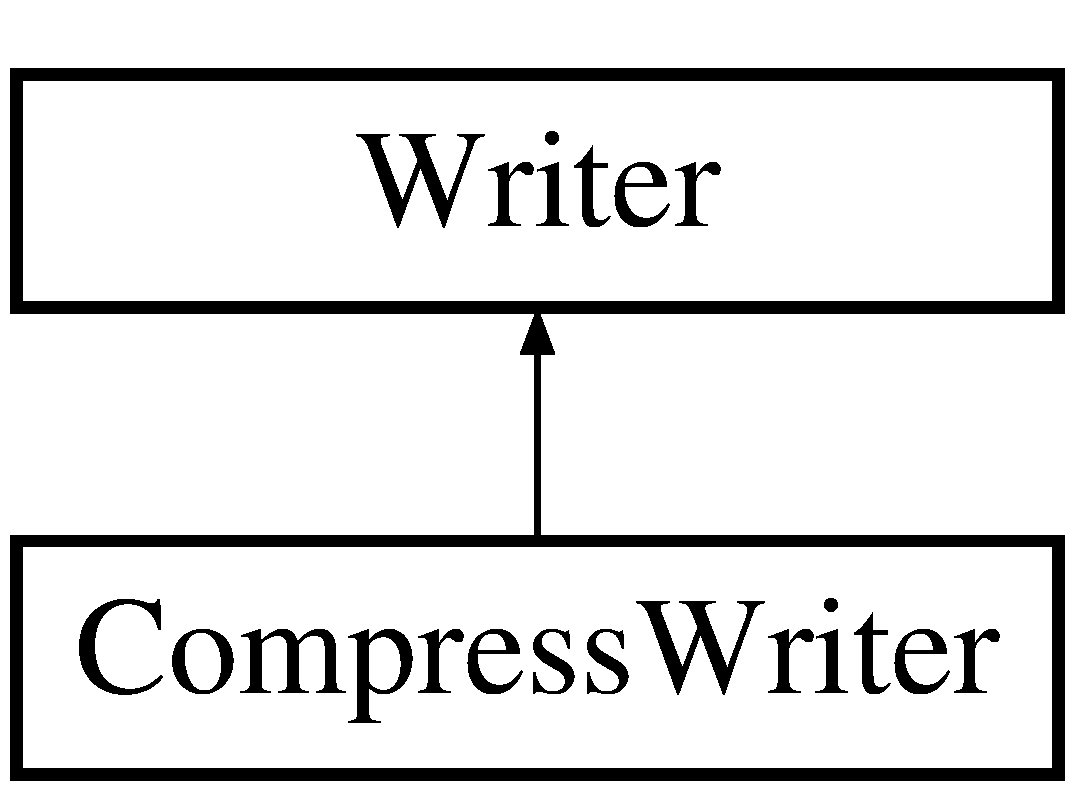
\includegraphics[height=2.000000cm]{classWriter}
\end{center}
\end{figure}
\subsection*{Public Member Functions}
\begin{DoxyCompactItemize}
\item 
\hyperlink{classWriter_aedc04cd5fb7b4b99d3ad906fef2116ce}{Writer} ()
\begin{DoxyCompactList}\small\item\em Write what the function does here. \end{DoxyCompactList}\item 
\hypertarget{classWriter_af731baeb537162d04d4925d0b505c39f}{{\bfseries Writer} (const \hyperlink{classWriter}{Writer} \&)=delete}\label{classWriter_af731baeb537162d04d4925d0b505c39f}

\item 
\hypertarget{classWriter_ab08fa23e717cff9212fe14489745a01b}{const \hyperlink{classWriter}{Writer} \& {\bfseries operator=} (const \hyperlink{classWriter}{Writer} \&)=delete}\label{classWriter_ab08fa23e717cff9212fe14489745a01b}

\item 
virtual \hyperlink{classWriter_ac1805972274066158c1a739a34b3428a}{$\sim$\+Writer} ()
\begin{DoxyCompactList}\small\item\em Write what the function does here. \end{DoxyCompactList}\item 
\hypertarget{classWriter_af9510dca900acf5724abb8225a55aaae}{virtual void {\bfseries write\+Byte} (uint8\+\_\+t)=0}\label{classWriter_af9510dca900acf5724abb8225a55aaae}

\item 
void \hyperlink{classWriter_ad8e295a99558edd8eeaf96ef56d6ab53}{write\+Bytes} (const uint8\+\_\+t $\ast$array, size\+\_\+t count)
\begin{DoxyCompactList}\small\item\em Write what the function does here. \end{DoxyCompactList}\item 
void \hyperlink{classWriter_a93d7ccb31453ec0f76ffe73b0ba6bb1b}{write\+U8} (uint8\+\_\+t v)
\begin{DoxyCompactList}\small\item\em Write what the function does here. \end{DoxyCompactList}\item 
void \hyperlink{classWriter_a26928e208d620cb69e8b1bbdce5f672b}{write\+S8} (int8\+\_\+t v)
\begin{DoxyCompactList}\small\item\em Write what the function does here. \end{DoxyCompactList}\item 
void \hyperlink{classWriter_a87898dff934c55c144149029173fe66f}{write\+U16} (uint16\+\_\+t v)
\begin{DoxyCompactList}\small\item\em Write what the function does here. \end{DoxyCompactList}\item 
void \hyperlink{classWriter_a8f83ddf72875fa45c2db077975717c02}{write\+S16} (int16\+\_\+t v)
\begin{DoxyCompactList}\small\item\em Write what the function does here. \end{DoxyCompactList}\item 
void \hyperlink{classWriter_ab8ed28096897dc429c95290542389224}{write\+U32} (uint32\+\_\+t v)
\begin{DoxyCompactList}\small\item\em Write what the function does here. \end{DoxyCompactList}\item 
void \hyperlink{classWriter_a6692f1d2ffa76a9acd3101af9fcdae23}{write\+S32} (int32\+\_\+t v)
\begin{DoxyCompactList}\small\item\em Write what the function does here. \end{DoxyCompactList}\item 
void \hyperlink{classWriter_aa2196ac25657790ad45fcd20e6fd8a3d}{write\+U64} (uint64\+\_\+t v)
\begin{DoxyCompactList}\small\item\em Write what the function does here. \end{DoxyCompactList}\item 
void \hyperlink{classWriter_a293a714331946c20921f8bdcaaf8fb45}{write\+S64} (int64\+\_\+t v)
\begin{DoxyCompactList}\small\item\em Write what the function does here. \end{DoxyCompactList}\item 
void \hyperlink{classWriter_a8816378c8b285c9c32e9ce852321bea6}{write\+F32} (float v)
\begin{DoxyCompactList}\small\item\em Write what the function does here. \end{DoxyCompactList}\item 
void \hyperlink{classWriter_ac3bd2e371437c63ff9a9d61be5578b7c}{write\+F64} (double v)
\begin{DoxyCompactList}\small\item\em Write what the function does here. \end{DoxyCompactList}\item 
void \hyperlink{classWriter_a473689a8f2ce7c1689db055fc7030773}{write\+Bool} (bool v)
\begin{DoxyCompactList}\small\item\em Write what the function does here. \end{DoxyCompactList}\item 
void \hyperlink{classWriter_aaab90e47e77581ec8aaab248c26e726e}{write\+String} (wstring v)
\begin{DoxyCompactList}\small\item\em Write what the function does here. \end{DoxyCompactList}\end{DoxyCompactItemize}


\subsection{Detailed Description}
Write what the function does here. 

\begin{DoxyReturn}{Returns}

\end{DoxyReturn}


Definition at line 574 of file stream.\+h.



\subsection{Constructor \& Destructor Documentation}
\hypertarget{classWriter_aedc04cd5fb7b4b99d3ad906fef2116ce}{\index{Writer@{Writer}!Writer@{Writer}}
\index{Writer@{Writer}!Writer@{Writer}}
\subsubsection[{Writer}]{\setlength{\rightskip}{0pt plus 5cm}Writer\+::\+Writer (
\begin{DoxyParamCaption}
{}
\end{DoxyParamCaption}
)\hspace{0.3cm}{\ttfamily [inline]}}}\label{classWriter_aedc04cd5fb7b4b99d3ad906fef2116ce}


Write what the function does here. 

\begin{DoxyReturn}{Returns}

\end{DoxyReturn}


Definition at line 583 of file stream.\+h.


\begin{DoxyCode}
584         \{
585         \}
\end{DoxyCode}
\hypertarget{classWriter_ac1805972274066158c1a739a34b3428a}{\index{Writer@{Writer}!````~Writer@{$\sim$\+Writer}}
\index{````~Writer@{$\sim$\+Writer}!Writer@{Writer}}
\subsubsection[{$\sim$\+Writer}]{\setlength{\rightskip}{0pt plus 5cm}virtual Writer\+::$\sim$\+Writer (
\begin{DoxyParamCaption}
{}
\end{DoxyParamCaption}
)\hspace{0.3cm}{\ttfamily [inline]}, {\ttfamily [virtual]}}}\label{classWriter_ac1805972274066158c1a739a34b3428a}


Write what the function does here. 

\begin{DoxyReturn}{Returns}

\end{DoxyReturn}


Definition at line 594 of file stream.\+h.


\begin{DoxyCode}
595         \{
596         \}
\end{DoxyCode}


\subsection{Member Function Documentation}
\hypertarget{classWriter_a473689a8f2ce7c1689db055fc7030773}{\index{Writer@{Writer}!write\+Bool@{write\+Bool}}
\index{write\+Bool@{write\+Bool}!Writer@{Writer}}
\subsubsection[{write\+Bool}]{\setlength{\rightskip}{0pt plus 5cm}void Writer\+::write\+Bool (
\begin{DoxyParamCaption}
\item[{bool}]{v}
\end{DoxyParamCaption}
)\hspace{0.3cm}{\ttfamily [inline]}}}\label{classWriter_a473689a8f2ce7c1689db055fc7030773}


Write what the function does here. 


\begin{DoxyParams}{Parameters}
{\em v} & \\
\hline
\end{DoxyParams}


Definition at line 752 of file stream.\+h.


\begin{DoxyCode}
753         \{
754             \hyperlink{classWriter_a93d7ccb31453ec0f76ffe73b0ba6bb1b}{writeU8}(v ? 1 : 0);
755         \}
\end{DoxyCode}
\hypertarget{classWriter_ad8e295a99558edd8eeaf96ef56d6ab53}{\index{Writer@{Writer}!write\+Bytes@{write\+Bytes}}
\index{write\+Bytes@{write\+Bytes}!Writer@{Writer}}
\subsubsection[{write\+Bytes}]{\setlength{\rightskip}{0pt plus 5cm}void Writer\+::write\+Bytes (
\begin{DoxyParamCaption}
\item[{const uint8\+\_\+t $\ast$}]{array, }
\item[{size\+\_\+t}]{count}
\end{DoxyParamCaption}
)\hspace{0.3cm}{\ttfamily [inline]}}}\label{classWriter_ad8e295a99558edd8eeaf96ef56d6ab53}


Write what the function does here. 

virtual void flush() \{ \}

/$\ast$$\ast$ Write what the function does here


\begin{DoxyParams}{Parameters}
{\em array} & \\
\hline
{\em count} & \\
\hline
\end{DoxyParams}


Definition at line 612 of file stream.\+h.


\begin{DoxyCode}
613         \{
614             \textcolor{keywordflow}{for}(\textcolor{keywordtype}{size\_t} i = 0; i < count; i++)
615                 writeByte(array[i]);
616         \}
\end{DoxyCode}
\hypertarget{classWriter_a8816378c8b285c9c32e9ce852321bea6}{\index{Writer@{Writer}!write\+F32@{write\+F32}}
\index{write\+F32@{write\+F32}!Writer@{Writer}}
\subsubsection[{write\+F32}]{\setlength{\rightskip}{0pt plus 5cm}void Writer\+::write\+F32 (
\begin{DoxyParamCaption}
\item[{float}]{v}
\end{DoxyParamCaption}
)\hspace{0.3cm}{\ttfamily [inline]}}}\label{classWriter_a8816378c8b285c9c32e9ce852321bea6}


Write what the function does here. 


\begin{DoxyParams}{Parameters}
{\em v} & \\
\hline
\end{DoxyParams}
Write what the function does here

\begin{DoxyReturn}{Returns}

\end{DoxyReturn}


Definition at line 706 of file stream.\+h.


\begin{DoxyCode}
707         \{
708             static\_assert(\textcolor{keyword}{sizeof}(\textcolor{keywordtype}{float}) == \textcolor{keyword}{sizeof}(uint32\_t), \textcolor{stringliteral}{"float is not 32 bits"});
709 \textcolor{comment}{}
710 \textcolor{comment}{            /**}
711 \textcolor{comment}{             * @brief Write what the function does here}
712 \textcolor{comment}{             *}
713 \textcolor{comment}{             * @return}
714 \textcolor{comment}{             **/}
715             \textcolor{keyword}{union}
716             \{
717                 uint32\_t ival;
718                 \textcolor{keywordtype}{float} fval;
719             \};
720             fval = v;
721             \hyperlink{classWriter_ab8ed28096897dc429c95290542389224}{writeU32}(ival);
722         \}
\end{DoxyCode}
\hypertarget{classWriter_ac3bd2e371437c63ff9a9d61be5578b7c}{\index{Writer@{Writer}!write\+F64@{write\+F64}}
\index{write\+F64@{write\+F64}!Writer@{Writer}}
\subsubsection[{write\+F64}]{\setlength{\rightskip}{0pt plus 5cm}void Writer\+::write\+F64 (
\begin{DoxyParamCaption}
\item[{double}]{v}
\end{DoxyParamCaption}
)\hspace{0.3cm}{\ttfamily [inline]}}}\label{classWriter_ac3bd2e371437c63ff9a9d61be5578b7c}


Write what the function does here. 


\begin{DoxyParams}{Parameters}
{\em v} & \\
\hline
\end{DoxyParams}
Write what the function does here

\begin{DoxyReturn}{Returns}

\end{DoxyReturn}


Definition at line 729 of file stream.\+h.


\begin{DoxyCode}
730         \{
731             static\_assert(\textcolor{keyword}{sizeof}(\textcolor{keywordtype}{double}) == \textcolor{keyword}{sizeof}(uint64\_t), \textcolor{stringliteral}{"double is not 64 bits"});
732 \textcolor{comment}{}
733 \textcolor{comment}{            /**}
734 \textcolor{comment}{             * @brief Write what the function does here}
735 \textcolor{comment}{             *}
736 \textcolor{comment}{             * @return}
737 \textcolor{comment}{             **/}
738             \textcolor{keyword}{union}
739             \{
740                 uint64\_t ival;
741                 \textcolor{keywordtype}{double} fval;
742             \};
743             fval = v;
744             \hyperlink{classWriter_aa2196ac25657790ad45fcd20e6fd8a3d}{writeU64}(ival);
745         \}
\end{DoxyCode}
\hypertarget{classWriter_a8f83ddf72875fa45c2db077975717c02}{\index{Writer@{Writer}!write\+S16@{write\+S16}}
\index{write\+S16@{write\+S16}!Writer@{Writer}}
\subsubsection[{write\+S16}]{\setlength{\rightskip}{0pt plus 5cm}void Writer\+::write\+S16 (
\begin{DoxyParamCaption}
\item[{int16\+\_\+t}]{v}
\end{DoxyParamCaption}
)\hspace{0.3cm}{\ttfamily [inline]}}}\label{classWriter_a8f83ddf72875fa45c2db077975717c02}


Write what the function does here. 


\begin{DoxyParams}{Parameters}
{\em v} & \\
\hline
\end{DoxyParams}


Definition at line 654 of file stream.\+h.


\begin{DoxyCode}
655         \{
656             \hyperlink{classWriter_a87898dff934c55c144149029173fe66f}{writeU16}(v);
657         \}
\end{DoxyCode}
\hypertarget{classWriter_a6692f1d2ffa76a9acd3101af9fcdae23}{\index{Writer@{Writer}!write\+S32@{write\+S32}}
\index{write\+S32@{write\+S32}!Writer@{Writer}}
\subsubsection[{write\+S32}]{\setlength{\rightskip}{0pt plus 5cm}void Writer\+::write\+S32 (
\begin{DoxyParamCaption}
\item[{int32\+\_\+t}]{v}
\end{DoxyParamCaption}
)\hspace{0.3cm}{\ttfamily [inline]}}}\label{classWriter_a6692f1d2ffa76a9acd3101af9fcdae23}


Write what the function does here. 


\begin{DoxyParams}{Parameters}
{\em v} & \\
\hline
\end{DoxyParams}


Definition at line 675 of file stream.\+h.


\begin{DoxyCode}
676         \{
677             \hyperlink{classWriter_ab8ed28096897dc429c95290542389224}{writeU32}(v);
678         \}
\end{DoxyCode}
\hypertarget{classWriter_a293a714331946c20921f8bdcaaf8fb45}{\index{Writer@{Writer}!write\+S64@{write\+S64}}
\index{write\+S64@{write\+S64}!Writer@{Writer}}
\subsubsection[{write\+S64}]{\setlength{\rightskip}{0pt plus 5cm}void Writer\+::write\+S64 (
\begin{DoxyParamCaption}
\item[{int64\+\_\+t}]{v}
\end{DoxyParamCaption}
)\hspace{0.3cm}{\ttfamily [inline]}}}\label{classWriter_a293a714331946c20921f8bdcaaf8fb45}


Write what the function does here. 


\begin{DoxyParams}{Parameters}
{\em v} & \\
\hline
\end{DoxyParams}


Definition at line 696 of file stream.\+h.


\begin{DoxyCode}
697         \{
698             \hyperlink{classWriter_aa2196ac25657790ad45fcd20e6fd8a3d}{writeU64}(v);
699         \}
\end{DoxyCode}
\hypertarget{classWriter_a26928e208d620cb69e8b1bbdce5f672b}{\index{Writer@{Writer}!write\+S8@{write\+S8}}
\index{write\+S8@{write\+S8}!Writer@{Writer}}
\subsubsection[{write\+S8}]{\setlength{\rightskip}{0pt plus 5cm}void Writer\+::write\+S8 (
\begin{DoxyParamCaption}
\item[{int8\+\_\+t}]{v}
\end{DoxyParamCaption}
)\hspace{0.3cm}{\ttfamily [inline]}}}\label{classWriter_a26928e208d620cb69e8b1bbdce5f672b}


Write what the function does here. 


\begin{DoxyParams}{Parameters}
{\em v} & \\
\hline
\end{DoxyParams}


Definition at line 633 of file stream.\+h.


\begin{DoxyCode}
634         \{
635             writeByte(v);
636         \}
\end{DoxyCode}
\hypertarget{classWriter_aaab90e47e77581ec8aaab248c26e726e}{\index{Writer@{Writer}!write\+String@{write\+String}}
\index{write\+String@{write\+String}!Writer@{Writer}}
\subsubsection[{write\+String}]{\setlength{\rightskip}{0pt plus 5cm}void Writer\+::write\+String (
\begin{DoxyParamCaption}
\item[{wstring}]{v}
\end{DoxyParamCaption}
)\hspace{0.3cm}{\ttfamily [inline]}}}\label{classWriter_aaab90e47e77581ec8aaab248c26e726e}


Write what the function does here. 


\begin{DoxyParams}{Parameters}
{\em v} & \\
\hline
\end{DoxyParams}


Definition at line 762 of file stream.\+h.


\begin{DoxyCode}
763         \{
764 
765             \textcolor{keywordflow}{for}(\textcolor{keywordtype}{size\_t} i = 0; i < v.length(); i++)
766             \{
767                 uint32\_t ch = v[i];
768 
769                 \textcolor{keywordflow}{if}(ch != 0 && ch < 0x80)
770                 \{
771                     \hyperlink{classWriter_a93d7ccb31453ec0f76ffe73b0ba6bb1b}{writeU8}(ch);
772                 \}
773 
774                 \textcolor{keywordflow}{else} \textcolor{keywordflow}{if}(ch < 0x800)
775                 \{
776                     \hyperlink{classWriter_a93d7ccb31453ec0f76ffe73b0ba6bb1b}{writeU8}(0xC0 | ((ch >> 6) & 0x1F));
777                     \hyperlink{classWriter_a93d7ccb31453ec0f76ffe73b0ba6bb1b}{writeU8}(0x80 | ((ch) & 0x3F));
778                 \}
779 
780                 \textcolor{keywordflow}{else} \textcolor{keywordflow}{if}(ch < 0x1000)
781                 \{
782                     \hyperlink{classWriter_a93d7ccb31453ec0f76ffe73b0ba6bb1b}{writeU8}(0xE0 | ((ch >> 12) & 0xF));
783                     \hyperlink{classWriter_a93d7ccb31453ec0f76ffe73b0ba6bb1b}{writeU8}(0x80 | ((ch >> 6) & 0x3F));
784                     \hyperlink{classWriter_a93d7ccb31453ec0f76ffe73b0ba6bb1b}{writeU8}(0x80 | ((ch) & 0x3F));
785                 \}
786 
787                 \textcolor{keywordflow}{else}
788                 \{
789                     \hyperlink{classWriter_a93d7ccb31453ec0f76ffe73b0ba6bb1b}{writeU8}(0xF0 | ((ch >> 18) & 0x7));
790                     \hyperlink{classWriter_a93d7ccb31453ec0f76ffe73b0ba6bb1b}{writeU8}(0x80 | ((ch >> 12) & 0x3F));
791                     \hyperlink{classWriter_a93d7ccb31453ec0f76ffe73b0ba6bb1b}{writeU8}(0x80 | ((ch >> 6) & 0x3F));
792                     \hyperlink{classWriter_a93d7ccb31453ec0f76ffe73b0ba6bb1b}{writeU8}(0x80 | ((ch) & 0x3F));
793                 \}
794             \}
795             \hyperlink{classWriter_a93d7ccb31453ec0f76ffe73b0ba6bb1b}{writeU8}(0);
796         \}
\end{DoxyCode}
\hypertarget{classWriter_a87898dff934c55c144149029173fe66f}{\index{Writer@{Writer}!write\+U16@{write\+U16}}
\index{write\+U16@{write\+U16}!Writer@{Writer}}
\subsubsection[{write\+U16}]{\setlength{\rightskip}{0pt plus 5cm}void Writer\+::write\+U16 (
\begin{DoxyParamCaption}
\item[{uint16\+\_\+t}]{v}
\end{DoxyParamCaption}
)\hspace{0.3cm}{\ttfamily [inline]}}}\label{classWriter_a87898dff934c55c144149029173fe66f}


Write what the function does here. 


\begin{DoxyParams}{Parameters}
{\em v} & \\
\hline
\end{DoxyParams}


Definition at line 643 of file stream.\+h.



Referenced by L\+Z77\+Code\+Type\+::write().


\begin{DoxyCode}
644         \{
645             \hyperlink{classWriter_a93d7ccb31453ec0f76ffe73b0ba6bb1b}{writeU8}((uint8\_t)(v >> 8));
646             \hyperlink{classWriter_a93d7ccb31453ec0f76ffe73b0ba6bb1b}{writeU8}((uint8\_t)(v & 0xFF));
647         \}
\end{DoxyCode}
\hypertarget{classWriter_ab8ed28096897dc429c95290542389224}{\index{Writer@{Writer}!write\+U32@{write\+U32}}
\index{write\+U32@{write\+U32}!Writer@{Writer}}
\subsubsection[{write\+U32}]{\setlength{\rightskip}{0pt plus 5cm}void Writer\+::write\+U32 (
\begin{DoxyParamCaption}
\item[{uint32\+\_\+t}]{v}
\end{DoxyParamCaption}
)\hspace{0.3cm}{\ttfamily [inline]}}}\label{classWriter_ab8ed28096897dc429c95290542389224}


Write what the function does here. 


\begin{DoxyParams}{Parameters}
{\em v} & \\
\hline
\end{DoxyParams}


Definition at line 664 of file stream.\+h.


\begin{DoxyCode}
665         \{
666             \hyperlink{classWriter_a87898dff934c55c144149029173fe66f}{writeU16}((uint16\_t)(v >> 16));
667             \hyperlink{classWriter_a87898dff934c55c144149029173fe66f}{writeU16}((uint16\_t)(v & 0xFFFF));
668         \}
\end{DoxyCode}
\hypertarget{classWriter_aa2196ac25657790ad45fcd20e6fd8a3d}{\index{Writer@{Writer}!write\+U64@{write\+U64}}
\index{write\+U64@{write\+U64}!Writer@{Writer}}
\subsubsection[{write\+U64}]{\setlength{\rightskip}{0pt plus 5cm}void Writer\+::write\+U64 (
\begin{DoxyParamCaption}
\item[{uint64\+\_\+t}]{v}
\end{DoxyParamCaption}
)\hspace{0.3cm}{\ttfamily [inline]}}}\label{classWriter_aa2196ac25657790ad45fcd20e6fd8a3d}


Write what the function does here. 


\begin{DoxyParams}{Parameters}
{\em v} & \\
\hline
\end{DoxyParams}


Definition at line 685 of file stream.\+h.


\begin{DoxyCode}
686         \{
687             \hyperlink{classWriter_ab8ed28096897dc429c95290542389224}{writeU32}((uint64\_t)(v >> 32));
688             \hyperlink{classWriter_ab8ed28096897dc429c95290542389224}{writeU32}((uint64\_t)(v & 0xFFFFFFFFU));
689         \}
\end{DoxyCode}
\hypertarget{classWriter_a93d7ccb31453ec0f76ffe73b0ba6bb1b}{\index{Writer@{Writer}!write\+U8@{write\+U8}}
\index{write\+U8@{write\+U8}!Writer@{Writer}}
\subsubsection[{write\+U8}]{\setlength{\rightskip}{0pt plus 5cm}void Writer\+::write\+U8 (
\begin{DoxyParamCaption}
\item[{uint8\+\_\+t}]{v}
\end{DoxyParamCaption}
)\hspace{0.3cm}{\ttfamily [inline]}}}\label{classWriter_a93d7ccb31453ec0f76ffe73b0ba6bb1b}


Write what the function does here. 


\begin{DoxyParams}{Parameters}
{\em v} & \\
\hline
\end{DoxyParams}


Definition at line 623 of file stream.\+h.


\begin{DoxyCode}
624         \{
625             writeByte(v);
626         \}
\end{DoxyCode}


The documentation for this class was generated from the following file\+:\begin{DoxyCompactItemize}
\item 
stream.\+h\end{DoxyCompactItemize}

\hypertarget{structWriterData}{\section{Writer\+Data Struct Reference}
\label{structWriterData}\index{Writer\+Data@{Writer\+Data}}
}
\subsection*{Public Attributes}
\begin{DoxyCompactItemize}
\item 
\hypertarget{structWriterData_a4dd9356d279d59559971ed4d0015228f}{\hyperlink{structSDL__EventQueue}{S\+D\+L\+\_\+\+Event\+Queue} $\ast$ {\bfseries queue}}\label{structWriterData_a4dd9356d279d59559971ed4d0015228f}

\item 
\hypertarget{structWriterData_a3b86410f4a64340f0e0c92e4274c953f}{int {\bfseries index}}\label{structWriterData_a3b86410f4a64340f0e0c92e4274c953f}

\item 
\hypertarget{structWriterData_a36d6ffb48f4089b190daccd62f2edfbf}{char {\bfseries padding1} \mbox{[}S\+D\+L\+\_\+\+C\+A\+C\+H\+E\+L\+I\+N\+E\+\_\+\+S\+I\+Z\+E-\/(sizeof(\hyperlink{structSDL__EventQueue}{S\+D\+L\+\_\+\+Event\+Queue} $\ast$)+sizeof(int))\%S\+D\+L\+\_\+\+C\+A\+C\+H\+E\+L\+I\+N\+E\+\_\+\+S\+I\+Z\+E\mbox{]}}\label{structWriterData_a36d6ffb48f4089b190daccd62f2edfbf}

\item 
\hypertarget{structWriterData_ac3554d71d52d39d4b972d74a9b67f678}{int {\bfseries waits}}\label{structWriterData_ac3554d71d52d39d4b972d74a9b67f678}

\item 
\hypertarget{structWriterData_ae97f71fc614c7d01fbb83fc3bd497617}{S\+D\+L\+\_\+bool {\bfseries lock\+\_\+free}}\label{structWriterData_ae97f71fc614c7d01fbb83fc3bd497617}

\item 
\hypertarget{structWriterData_a47f79e859ec21455f9d18b2e1198c8ca}{char {\bfseries padding2} \mbox{[}S\+D\+L\+\_\+\+C\+A\+C\+H\+E\+L\+I\+N\+E\+\_\+\+S\+I\+Z\+E-\/sizeof(int)-\/sizeof(S\+D\+L\+\_\+bool)\mbox{]}}\label{structWriterData_a47f79e859ec21455f9d18b2e1198c8ca}

\end{DoxyCompactItemize}


\subsection{Detailed Description}


Definition at line 478 of file testatomic.\+c.



The documentation for this struct was generated from the following file\+:\begin{DoxyCompactItemize}
\item 
S\+D\+L2-\/2.\+0.\+3/test/testatomic.\+c\end{DoxyCompactItemize}

\hypertarget{structz__stream__s}{\section{z\+\_\+stream\+\_\+s Struct Reference}
\label{structz__stream__s}\index{z\+\_\+stream\+\_\+s@{z\+\_\+stream\+\_\+s}}
}
\subsection*{Public Attributes}
\begin{DoxyCompactItemize}
\item 
\hypertarget{structz__stream__s_a21d2c026f0f2fcd67f33011231f8ed00}{Bytef $\ast$ {\bfseries next\+\_\+in}}\label{structz__stream__s_a21d2c026f0f2fcd67f33011231f8ed00}

\item 
\hypertarget{structz__stream__s_a0cf177f50dbb49692f27480cbcfde794}{u\+Int {\bfseries avail\+\_\+in}}\label{structz__stream__s_a0cf177f50dbb49692f27480cbcfde794}

\item 
\hypertarget{structz__stream__s_aa8f408b9632737dc21519fa1ed34b08d}{u\+Long {\bfseries total\+\_\+in}}\label{structz__stream__s_aa8f408b9632737dc21519fa1ed34b08d}

\item 
\hypertarget{structz__stream__s_aed4a02cfe93e975314fed50b04427bf3}{Bytef $\ast$ {\bfseries next\+\_\+out}}\label{structz__stream__s_aed4a02cfe93e975314fed50b04427bf3}

\item 
\hypertarget{structz__stream__s_a45ad2364307af9d944fd39d4eca3ca3c}{u\+Int {\bfseries avail\+\_\+out}}\label{structz__stream__s_a45ad2364307af9d944fd39d4eca3ca3c}

\item 
\hypertarget{structz__stream__s_abae26f1f236cf920250b9d37fdf009c1}{u\+Long {\bfseries total\+\_\+out}}\label{structz__stream__s_abae26f1f236cf920250b9d37fdf009c1}

\item 
\hypertarget{structz__stream__s_a9b2f745fc780e3b33e2935f8c650a326}{char $\ast$ {\bfseries msg}}\label{structz__stream__s_a9b2f745fc780e3b33e2935f8c650a326}

\item 
\hypertarget{structz__stream__s_ac4a114217a1868dc6fbe7d1f5bda126b}{struct \hyperlink{structinternal__state}{internal\+\_\+state} F\+A\+R $\ast$ {\bfseries state}}\label{structz__stream__s_ac4a114217a1868dc6fbe7d1f5bda126b}

\item 
\hypertarget{structz__stream__s_a23a2299c384f808e76e9908f21216b0f}{alloc\+\_\+func {\bfseries zalloc}}\label{structz__stream__s_a23a2299c384f808e76e9908f21216b0f}

\item 
\hypertarget{structz__stream__s_a89eb750ade7f4f0b56bfdadf13344982}{free\+\_\+func {\bfseries zfree}}\label{structz__stream__s_a89eb750ade7f4f0b56bfdadf13344982}

\item 
\hypertarget{structz__stream__s_ab72467f908d2ce65d5b42ee6556ef8bb}{voidpf {\bfseries opaque}}\label{structz__stream__s_ab72467f908d2ce65d5b42ee6556ef8bb}

\item 
\hypertarget{structz__stream__s_a9d8f63877d7639a8bca60f9fc3704fc4}{int {\bfseries data\+\_\+type}}\label{structz__stream__s_a9d8f63877d7639a8bca60f9fc3704fc4}

\item 
\hypertarget{structz__stream__s_ade2217fe31e671be1257731883201223}{u\+Long {\bfseries adler}}\label{structz__stream__s_ade2217fe31e671be1257731883201223}

\item 
\hypertarget{structz__stream__s_add73791dd19b49c9c68f3f3d328c37db}{u\+Long {\bfseries reserved}}\label{structz__stream__s_add73791dd19b49c9c68f3f3d328c37db}

\end{DoxyCompactItemize}


\subsection{Detailed Description}


Definition at line 82 of file zlib.\+h.



The documentation for this struct was generated from the following file\+:\begin{DoxyCompactItemize}
\item 
zlib.\+h\end{DoxyCompactItemize}

\chapter{File Documentation}
\hypertarget{SDL__active_8h}{\section{codeblocks/include/\+S\+D\+L/\+S\+D\+L\+\_\+active.h File Reference}
\label{SDL__active_8h}\index{codeblocks/include/\+S\+D\+L/\+S\+D\+L\+\_\+active.\+h@{codeblocks/include/\+S\+D\+L/\+S\+D\+L\+\_\+active.\+h}}
}
{\ttfamily \#include \char`\"{}S\+D\+L\+\_\+stdinc.\+h\char`\"{}}\\*
{\ttfamily \#include \char`\"{}S\+D\+L\+\_\+error.\+h\char`\"{}}\\*
{\ttfamily \#include \char`\"{}begin\+\_\+code.\+h\char`\"{}}\\*
{\ttfamily \#include \char`\"{}close\+\_\+code.\+h\char`\"{}}\\*
\subsection*{Macros}
\begin{Indent}{\bf The available application states}\par
\begin{DoxyCompactItemize}
\item 
\#define \hyperlink{SDL__active_8h_adbb0da5a3196e16a2104a8dd4d048177}{S\+D\+L\+\_\+\+A\+P\+P\+M\+O\+U\+S\+E\+F\+O\+C\+U\+S}~0x01
\item 
\#define \hyperlink{SDL__active_8h_ac41cbb6cae92292898f29b6e6338d5a6}{S\+D\+L\+\_\+\+A\+P\+P\+I\+N\+P\+U\+T\+F\+O\+C\+U\+S}~0x02
\item 
\#define \hyperlink{SDL__active_8h_a54820fe5c98fa3369dfad1f13c76cb4f}{S\+D\+L\+\_\+\+A\+P\+P\+A\+C\+T\+I\+V\+E}~0x04
\end{DoxyCompactItemize}
\end{Indent}
\subsection*{Functions}
\begin{DoxyCompactItemize}
\item 
D\+E\+C\+L\+S\+P\+E\+C Uint8 S\+D\+L\+C\+A\+L\+L \hyperlink{SDL__active_8h_a33e36b26e1d6c532e4a325188473a104}{S\+D\+L\+\_\+\+Get\+App\+State} (void)
\end{DoxyCompactItemize}


\subsection{Detailed Description}
Include file for S\+D\+L application focus event handling 

Definition in file \hyperlink{SDL__active_8h_source}{S\+D\+L\+\_\+active.\+h}.



\subsection{Macro Definition Documentation}
\hypertarget{SDL__active_8h_a54820fe5c98fa3369dfad1f13c76cb4f}{\index{S\+D\+L\+\_\+active.\+h@{S\+D\+L\+\_\+active.\+h}!S\+D\+L\+\_\+\+A\+P\+P\+A\+C\+T\+I\+V\+E@{S\+D\+L\+\_\+\+A\+P\+P\+A\+C\+T\+I\+V\+E}}
\index{S\+D\+L\+\_\+\+A\+P\+P\+A\+C\+T\+I\+V\+E@{S\+D\+L\+\_\+\+A\+P\+P\+A\+C\+T\+I\+V\+E}!S\+D\+L\+\_\+active.\+h@{S\+D\+L\+\_\+active.\+h}}
\subsubsection[{S\+D\+L\+\_\+\+A\+P\+P\+A\+C\+T\+I\+V\+E}]{\setlength{\rightskip}{0pt plus 5cm}\#define S\+D\+L\+\_\+\+A\+P\+P\+A\+C\+T\+I\+V\+E~0x04}}\label{SDL__active_8h_a54820fe5c98fa3369dfad1f13c76cb4f}
The application is active 

Definition at line 44 of file S\+D\+L\+\_\+active.\+h.

\hypertarget{SDL__active_8h_ac41cbb6cae92292898f29b6e6338d5a6}{\index{S\+D\+L\+\_\+active.\+h@{S\+D\+L\+\_\+active.\+h}!S\+D\+L\+\_\+\+A\+P\+P\+I\+N\+P\+U\+T\+F\+O\+C\+U\+S@{S\+D\+L\+\_\+\+A\+P\+P\+I\+N\+P\+U\+T\+F\+O\+C\+U\+S}}
\index{S\+D\+L\+\_\+\+A\+P\+P\+I\+N\+P\+U\+T\+F\+O\+C\+U\+S@{S\+D\+L\+\_\+\+A\+P\+P\+I\+N\+P\+U\+T\+F\+O\+C\+U\+S}!S\+D\+L\+\_\+active.\+h@{S\+D\+L\+\_\+active.\+h}}
\subsubsection[{S\+D\+L\+\_\+\+A\+P\+P\+I\+N\+P\+U\+T\+F\+O\+C\+U\+S}]{\setlength{\rightskip}{0pt plus 5cm}\#define S\+D\+L\+\_\+\+A\+P\+P\+I\+N\+P\+U\+T\+F\+O\+C\+U\+S~0x02}}\label{SDL__active_8h_ac41cbb6cae92292898f29b6e6338d5a6}
The app has input focus 

Definition at line 43 of file S\+D\+L\+\_\+active.\+h.

\hypertarget{SDL__active_8h_adbb0da5a3196e16a2104a8dd4d048177}{\index{S\+D\+L\+\_\+active.\+h@{S\+D\+L\+\_\+active.\+h}!S\+D\+L\+\_\+\+A\+P\+P\+M\+O\+U\+S\+E\+F\+O\+C\+U\+S@{S\+D\+L\+\_\+\+A\+P\+P\+M\+O\+U\+S\+E\+F\+O\+C\+U\+S}}
\index{S\+D\+L\+\_\+\+A\+P\+P\+M\+O\+U\+S\+E\+F\+O\+C\+U\+S@{S\+D\+L\+\_\+\+A\+P\+P\+M\+O\+U\+S\+E\+F\+O\+C\+U\+S}!S\+D\+L\+\_\+active.\+h@{S\+D\+L\+\_\+active.\+h}}
\subsubsection[{S\+D\+L\+\_\+\+A\+P\+P\+M\+O\+U\+S\+E\+F\+O\+C\+U\+S}]{\setlength{\rightskip}{0pt plus 5cm}\#define S\+D\+L\+\_\+\+A\+P\+P\+M\+O\+U\+S\+E\+F\+O\+C\+U\+S~0x01}}\label{SDL__active_8h_adbb0da5a3196e16a2104a8dd4d048177}
The app has mouse coverage 

Definition at line 42 of file S\+D\+L\+\_\+active.\+h.



\subsection{Function Documentation}
\hypertarget{SDL__active_8h_a33e36b26e1d6c532e4a325188473a104}{\index{S\+D\+L\+\_\+active.\+h@{S\+D\+L\+\_\+active.\+h}!S\+D\+L\+\_\+\+Get\+App\+State@{S\+D\+L\+\_\+\+Get\+App\+State}}
\index{S\+D\+L\+\_\+\+Get\+App\+State@{S\+D\+L\+\_\+\+Get\+App\+State}!S\+D\+L\+\_\+active.\+h@{S\+D\+L\+\_\+active.\+h}}
\subsubsection[{S\+D\+L\+\_\+\+Get\+App\+State}]{\setlength{\rightskip}{0pt plus 5cm}D\+E\+C\+L\+S\+P\+E\+C Uint8 S\+D\+L\+C\+A\+L\+L S\+D\+L\+\_\+\+Get\+App\+State (
\begin{DoxyParamCaption}
\item[{void}]{}
\end{DoxyParamCaption}
)}}\label{SDL__active_8h_a33e36b26e1d6c532e4a325188473a104}
This function returns the current state of the application, which is a bitwise combination of S\+D\+L\+\_\+\+A\+P\+P\+M\+O\+U\+S\+E\+F\+O\+C\+U\+S, S\+D\+L\+\_\+\+A\+P\+P\+I\+N\+P\+U\+T\+F\+O\+C\+U\+S, and S\+D\+L\+\_\+\+A\+P\+P\+A\+C\+T\+I\+V\+E. If S\+D\+L\+\_\+\+A\+P\+P\+A\+C\+T\+I\+V\+E is set, then the user is able to see your application, otherwise it has been iconified or disabled. 
\hypertarget{SDL__byteorder_8h}{\section{codeblocks/include/\+S\+D\+L/\+S\+D\+L\+\_\+byteorder.h File Reference}
\label{SDL__byteorder_8h}\index{codeblocks/include/\+S\+D\+L/\+S\+D\+L\+\_\+byteorder.\+h@{codeblocks/include/\+S\+D\+L/\+S\+D\+L\+\_\+byteorder.\+h}}
}
{\ttfamily \#include \char`\"{}S\+D\+L\+\_\+endian.\+h\char`\"{}}\\*


\subsection{Detailed Description}
\begin{DoxyRefDesc}{Deprecated}
\item[\hyperlink{deprecated__deprecated000001}{Deprecated}]Use S\+D\+L\+\_\+endian.\+h instead \end{DoxyRefDesc}


Definition in file \hyperlink{SDL__byteorder_8h_source}{S\+D\+L\+\_\+byteorder.\+h}.


\hypertarget{SDL__cdrom_8h}{\section{codeblocks/include/\+S\+D\+L/\+S\+D\+L\+\_\+cdrom.h File Reference}
\label{SDL__cdrom_8h}\index{codeblocks/include/\+S\+D\+L/\+S\+D\+L\+\_\+cdrom.\+h@{codeblocks/include/\+S\+D\+L/\+S\+D\+L\+\_\+cdrom.\+h}}
}
{\ttfamily \#include \char`\"{}S\+D\+L\+\_\+stdinc.\+h\char`\"{}}\\*
{\ttfamily \#include \char`\"{}S\+D\+L\+\_\+error.\+h\char`\"{}}\\*
{\ttfamily \#include \char`\"{}begin\+\_\+code.\+h\char`\"{}}\\*
{\ttfamily \#include \char`\"{}close\+\_\+code.\+h\char`\"{}}\\*
\subsection*{Classes}
\begin{DoxyCompactItemize}
\item 
struct \hyperlink{structSDL__CDtrack}{S\+D\+L\+\_\+\+C\+Dtrack}
\item 
struct \hyperlink{structSDL__CD}{S\+D\+L\+\_\+\+C\+D}
\end{DoxyCompactItemize}
\subsection*{Macros}
\begin{DoxyCompactItemize}
\item 
\#define \hyperlink{SDL__cdrom_8h_a39eb10e45614b6b607fe7649c9dd75da}{S\+D\+L\+\_\+\+M\+A\+X\+\_\+\+T\+R\+A\+C\+K\+S}~99
\item 
\#define \hyperlink{SDL__cdrom_8h_a124d20fb441acc8db9f838ddef5864f5}{C\+D\+\_\+\+I\+N\+D\+R\+I\+V\+E}(status)~((int)(status) $>$ 0)
\end{DoxyCompactItemize}
\begin{Indent}{\bf Track Types}\par
{\em The types of C\+D-\/\+R\+O\+M track possible }\begin{DoxyCompactItemize}
\item 
\hypertarget{SDL__cdrom_8h_ad6442a4d4fceea628912110513f66bb4}{\#define {\bfseries S\+D\+L\+\_\+\+A\+U\+D\+I\+O\+\_\+\+T\+R\+A\+C\+K}~0x00}\label{SDL__cdrom_8h_ad6442a4d4fceea628912110513f66bb4}

\item 
\hypertarget{SDL__cdrom_8h_a9ca198a0fb15cf28ca1b0516e8118a14}{\#define {\bfseries S\+D\+L\+\_\+\+D\+A\+T\+A\+\_\+\+T\+R\+A\+C\+K}~0x04}\label{SDL__cdrom_8h_a9ca198a0fb15cf28ca1b0516e8118a14}

\end{DoxyCompactItemize}
\end{Indent}
\begin{Indent}{\bf Frames / M\+S\+F Conversion Functions}\par
{\em Conversion functions from frames to Minute/\+Second/\+Frames and vice versa }\begin{DoxyCompactItemize}
\item 
\hypertarget{SDL__cdrom_8h_a911576d3f90250544bf5376c52f9cb6f}{\#define {\bfseries C\+D\+\_\+\+F\+P\+S}~75}\label{SDL__cdrom_8h_a911576d3f90250544bf5376c52f9cb6f}

\item 
\#define {\bfseries F\+R\+A\+M\+E\+S\+\_\+\+T\+O\+\_\+\+M\+S\+F}(f, M, S, F)
\item 
\hypertarget{SDL__cdrom_8h_a4a715d6b5827deeae6629aaec24a3453}{\#define {\bfseries M\+S\+F\+\_\+\+T\+O\+\_\+\+F\+R\+A\+M\+E\+S}(M, S, F)~((M)$\ast$60$\ast$C\+D\+\_\+\+F\+P\+S+(S)$\ast$C\+D\+\_\+\+F\+P\+S+(F))}\label{SDL__cdrom_8h_a4a715d6b5827deeae6629aaec24a3453}

\end{DoxyCompactItemize}
\end{Indent}
\subsection*{Typedefs}
\begin{DoxyCompactItemize}
\item 
\hypertarget{SDL__cdrom_8h_af9d80a202083920dd939bbd7c7482581}{typedef struct \hyperlink{structSDL__CDtrack}{S\+D\+L\+\_\+\+C\+Dtrack} {\bfseries S\+D\+L\+\_\+\+C\+Dtrack}}\label{SDL__cdrom_8h_af9d80a202083920dd939bbd7c7482581}

\item 
typedef struct \hyperlink{structSDL__CD}{S\+D\+L\+\_\+\+C\+D} \hyperlink{SDL__cdrom_8h_a935dd4f32061b4ce72d9bf7c9175893a}{S\+D\+L\+\_\+\+C\+D}
\end{DoxyCompactItemize}
\subsection*{Enumerations}
\begin{DoxyCompactItemize}
\item 
enum \hyperlink{SDL__cdrom_8h_ae689551deb9bd434bce7e4c39e45e15d}{C\+Dstatus} \{ \\*
{\bfseries C\+D\+\_\+\+T\+R\+A\+Y\+E\+M\+P\+T\+Y}, 
{\bfseries C\+D\+\_\+\+S\+T\+O\+P\+P\+E\+D}, 
{\bfseries C\+D\+\_\+\+P\+L\+A\+Y\+I\+N\+G}, 
{\bfseries C\+D\+\_\+\+P\+A\+U\+S\+E\+D}, 
\\*
{\bfseries C\+D\+\_\+\+E\+R\+R\+O\+R} = -\/1
 \}
\end{DoxyCompactItemize}
\subsection*{Functions}
\begin{DoxyCompactItemize}
\item 
D\+E\+C\+L\+S\+P\+E\+C int S\+D\+L\+C\+A\+L\+L \hyperlink{SDL__cdrom_8h_a1d068354396e0f955b181dbf368bdd2f}{S\+D\+L\+\_\+\+C\+D\+Num\+Drives} (void)
\item 
D\+E\+C\+L\+S\+P\+E\+C const char $\ast$S\+D\+L\+C\+A\+L\+L \hyperlink{SDL__cdrom_8h_a7aeb8d2057662eb65cc26d2fabc3897f}{S\+D\+L\+\_\+\+C\+D\+Name} (int drive)
\item 
D\+E\+C\+L\+S\+P\+E\+C \hyperlink{structSDL__CD}{S\+D\+L\+\_\+\+C\+D} $\ast$S\+D\+L\+C\+A\+L\+L \hyperlink{SDL__cdrom_8h_aa19b41f1ed97048eaf888e2fc7141707}{S\+D\+L\+\_\+\+C\+D\+Open} (int drive)
\item 
D\+E\+C\+L\+S\+P\+E\+C \hyperlink{SDL__cdrom_8h_ae689551deb9bd434bce7e4c39e45e15d}{C\+Dstatus} S\+D\+L\+C\+A\+L\+L \hyperlink{SDL__cdrom_8h_a696066cb9444206195dfad7f77f2b38c}{S\+D\+L\+\_\+\+C\+D\+Status} (\hyperlink{structSDL__CD}{S\+D\+L\+\_\+\+C\+D} $\ast$cdrom)
\item 
D\+E\+C\+L\+S\+P\+E\+C int S\+D\+L\+C\+A\+L\+L \hyperlink{SDL__cdrom_8h_ad691acb785f309d632222573eda0957d}{S\+D\+L\+\_\+\+C\+D\+Play\+Tracks} (\hyperlink{structSDL__CD}{S\+D\+L\+\_\+\+C\+D} $\ast$cdrom, int start\+\_\+track, int start\+\_\+frame, int ntracks, int nframes)
\item 
D\+E\+C\+L\+S\+P\+E\+C int S\+D\+L\+C\+A\+L\+L \hyperlink{SDL__cdrom_8h_a993353ee8a87cb4e872a518d8cfaf6ca}{S\+D\+L\+\_\+\+C\+D\+Play} (\hyperlink{structSDL__CD}{S\+D\+L\+\_\+\+C\+D} $\ast$cdrom, int start, int length)
\item 
D\+E\+C\+L\+S\+P\+E\+C int S\+D\+L\+C\+A\+L\+L \hyperlink{SDL__cdrom_8h_a87dad4514f89a7e0df5166daf5d41755}{S\+D\+L\+\_\+\+C\+D\+Pause} (\hyperlink{structSDL__CD}{S\+D\+L\+\_\+\+C\+D} $\ast$cdrom)
\item 
D\+E\+C\+L\+S\+P\+E\+C int S\+D\+L\+C\+A\+L\+L \hyperlink{SDL__cdrom_8h_a345e19cb56b38baaa56e521a16194cfa}{S\+D\+L\+\_\+\+C\+D\+Resume} (\hyperlink{structSDL__CD}{S\+D\+L\+\_\+\+C\+D} $\ast$cdrom)
\item 
D\+E\+C\+L\+S\+P\+E\+C int S\+D\+L\+C\+A\+L\+L \hyperlink{SDL__cdrom_8h_afe244b2c7a9cb3fbc6c3fb96b373f9b2}{S\+D\+L\+\_\+\+C\+D\+Stop} (\hyperlink{structSDL__CD}{S\+D\+L\+\_\+\+C\+D} $\ast$cdrom)
\item 
D\+E\+C\+L\+S\+P\+E\+C int S\+D\+L\+C\+A\+L\+L \hyperlink{SDL__cdrom_8h_a7af6a6e13e9994156995f836e2724ac1}{S\+D\+L\+\_\+\+C\+D\+Eject} (\hyperlink{structSDL__CD}{S\+D\+L\+\_\+\+C\+D} $\ast$cdrom)
\item 
D\+E\+C\+L\+S\+P\+E\+C void S\+D\+L\+C\+A\+L\+L \hyperlink{SDL__cdrom_8h_aa6e4eae7d3d48fc247e15abf7edcc246}{S\+D\+L\+\_\+\+C\+D\+Close} (\hyperlink{structSDL__CD}{S\+D\+L\+\_\+\+C\+D} $\ast$cdrom)
\end{DoxyCompactItemize}


\subsection{Detailed Description}
This is the C\+D-\/audio control A\+P\+I for Simple Direct\+Media Layer

In order to use these functions, S\+D\+L\+\_\+\+Init() must have been called with the S\+D\+L\+\_\+\+I\+N\+I\+T\+\_\+\+C\+D\+R\+O\+M flag. This causes S\+D\+L to scan the system for C\+D-\/\+R\+O\+M drives, and load appropriate drivers. 

Definition in file \hyperlink{SDL__cdrom_8h_source}{S\+D\+L\+\_\+cdrom.\+h}.



\subsection{Macro Definition Documentation}
\hypertarget{SDL__cdrom_8h_a124d20fb441acc8db9f838ddef5864f5}{\index{S\+D\+L\+\_\+cdrom.\+h@{S\+D\+L\+\_\+cdrom.\+h}!C\+D\+\_\+\+I\+N\+D\+R\+I\+V\+E@{C\+D\+\_\+\+I\+N\+D\+R\+I\+V\+E}}
\index{C\+D\+\_\+\+I\+N\+D\+R\+I\+V\+E@{C\+D\+\_\+\+I\+N\+D\+R\+I\+V\+E}!S\+D\+L\+\_\+cdrom.\+h@{S\+D\+L\+\_\+cdrom.\+h}}
\subsubsection[{C\+D\+\_\+\+I\+N\+D\+R\+I\+V\+E}]{\setlength{\rightskip}{0pt plus 5cm}\#define C\+D\+\_\+\+I\+N\+D\+R\+I\+V\+E(
\begin{DoxyParamCaption}
\item[{}]{status}
\end{DoxyParamCaption}
)~((int)(status) $>$ 0)}}\label{SDL__cdrom_8h_a124d20fb441acc8db9f838ddef5864f5}
Given a status, returns true if there's a disk in the drive 

Definition at line 68 of file S\+D\+L\+\_\+cdrom.\+h.

\hypertarget{SDL__cdrom_8h_adb3ec0ecef53497f305d77c66018dbfd}{\index{S\+D\+L\+\_\+cdrom.\+h@{S\+D\+L\+\_\+cdrom.\+h}!F\+R\+A\+M\+E\+S\+\_\+\+T\+O\+\_\+\+M\+S\+F@{F\+R\+A\+M\+E\+S\+\_\+\+T\+O\+\_\+\+M\+S\+F}}
\index{F\+R\+A\+M\+E\+S\+\_\+\+T\+O\+\_\+\+M\+S\+F@{F\+R\+A\+M\+E\+S\+\_\+\+T\+O\+\_\+\+M\+S\+F}!S\+D\+L\+\_\+cdrom.\+h@{S\+D\+L\+\_\+cdrom.\+h}}
\subsubsection[{F\+R\+A\+M\+E\+S\+\_\+\+T\+O\+\_\+\+M\+S\+F}]{\setlength{\rightskip}{0pt plus 5cm}\#define F\+R\+A\+M\+E\+S\+\_\+\+T\+O\+\_\+\+M\+S\+F(
\begin{DoxyParamCaption}
\item[{}]{f, }
\item[{}]{M, }
\item[{}]{S, }
\item[{}]{F}
\end{DoxyParamCaption}
)}}\label{SDL__cdrom_8h_adb3ec0ecef53497f305d77c66018dbfd}
{\bfseries Value\+:}
\begin{DoxyCode}
\{                   \(\backslash\)
    int value = f;                          \(\backslash\)
    *(F) = value%CD\_FPS;                        \(\backslash\)
    value /= CD\_FPS;                        \(\backslash\)
    *(S) = value%60;                        \(\backslash\)
    value /= 60;                            \(\backslash\)
    *(M) = value;                           \(\backslash\)
\}
\end{DoxyCode}


Definition at line 97 of file S\+D\+L\+\_\+cdrom.\+h.

\hypertarget{SDL__cdrom_8h_a39eb10e45614b6b607fe7649c9dd75da}{\index{S\+D\+L\+\_\+cdrom.\+h@{S\+D\+L\+\_\+cdrom.\+h}!S\+D\+L\+\_\+\+M\+A\+X\+\_\+\+T\+R\+A\+C\+K\+S@{S\+D\+L\+\_\+\+M\+A\+X\+\_\+\+T\+R\+A\+C\+K\+S}}
\index{S\+D\+L\+\_\+\+M\+A\+X\+\_\+\+T\+R\+A\+C\+K\+S@{S\+D\+L\+\_\+\+M\+A\+X\+\_\+\+T\+R\+A\+C\+K\+S}!S\+D\+L\+\_\+cdrom.\+h@{S\+D\+L\+\_\+cdrom.\+h}}
\subsubsection[{S\+D\+L\+\_\+\+M\+A\+X\+\_\+\+T\+R\+A\+C\+K\+S}]{\setlength{\rightskip}{0pt plus 5cm}\#define S\+D\+L\+\_\+\+M\+A\+X\+\_\+\+T\+R\+A\+C\+K\+S~99}}\label{SDL__cdrom_8h_a39eb10e45614b6b607fe7649c9dd75da}
The maximum number of C\+D-\/\+R\+O\+M tracks on a disk 

Definition at line 48 of file S\+D\+L\+\_\+cdrom.\+h.



\subsection{Typedef Documentation}
\hypertarget{SDL__cdrom_8h_a935dd4f32061b4ce72d9bf7c9175893a}{\index{S\+D\+L\+\_\+cdrom.\+h@{S\+D\+L\+\_\+cdrom.\+h}!S\+D\+L\+\_\+\+C\+D@{S\+D\+L\+\_\+\+C\+D}}
\index{S\+D\+L\+\_\+\+C\+D@{S\+D\+L\+\_\+\+C\+D}!S\+D\+L\+\_\+cdrom.\+h@{S\+D\+L\+\_\+cdrom.\+h}}
\subsubsection[{S\+D\+L\+\_\+\+C\+D}]{\setlength{\rightskip}{0pt plus 5cm}typedef struct {\bf S\+D\+L\+\_\+\+C\+D}  {\bf S\+D\+L\+\_\+\+C\+D}}}\label{SDL__cdrom_8h_a935dd4f32061b4ce72d9bf7c9175893a}
This structure is only current as of the last call to \hyperlink{SDL__cdrom_8h_a696066cb9444206195dfad7f77f2b38c}{S\+D\+L\+\_\+\+C\+D\+Status()} 

\subsection{Enumeration Type Documentation}
\hypertarget{SDL__cdrom_8h_ae689551deb9bd434bce7e4c39e45e15d}{\index{S\+D\+L\+\_\+cdrom.\+h@{S\+D\+L\+\_\+cdrom.\+h}!C\+Dstatus@{C\+Dstatus}}
\index{C\+Dstatus@{C\+Dstatus}!S\+D\+L\+\_\+cdrom.\+h@{S\+D\+L\+\_\+cdrom.\+h}}
\subsubsection[{C\+Dstatus}]{\setlength{\rightskip}{0pt plus 5cm}enum {\bf C\+Dstatus}}}\label{SDL__cdrom_8h_ae689551deb9bd434bce7e4c39e45e15d}
The possible states which a C\+D-\/\+R\+O\+M drive can be in. 

Definition at line 59 of file S\+D\+L\+\_\+cdrom.\+h.


\begin{DoxyCode}
59              \{
60     CD\_TRAYEMPTY,
61     CD\_STOPPED,
62     CD\_PLAYING,
63     CD\_PAUSED,
64     CD\_ERROR = -1
65 \} \hyperlink{SDL__cdrom_8h_ae689551deb9bd434bce7e4c39e45e15d}{CDstatus};
\end{DoxyCode}


\subsection{Function Documentation}
\hypertarget{SDL__cdrom_8h_aa6e4eae7d3d48fc247e15abf7edcc246}{\index{S\+D\+L\+\_\+cdrom.\+h@{S\+D\+L\+\_\+cdrom.\+h}!S\+D\+L\+\_\+\+C\+D\+Close@{S\+D\+L\+\_\+\+C\+D\+Close}}
\index{S\+D\+L\+\_\+\+C\+D\+Close@{S\+D\+L\+\_\+\+C\+D\+Close}!S\+D\+L\+\_\+cdrom.\+h@{S\+D\+L\+\_\+cdrom.\+h}}
\subsubsection[{S\+D\+L\+\_\+\+C\+D\+Close}]{\setlength{\rightskip}{0pt plus 5cm}D\+E\+C\+L\+S\+P\+E\+C void S\+D\+L\+C\+A\+L\+L S\+D\+L\+\_\+\+C\+D\+Close (
\begin{DoxyParamCaption}
\item[{{\bf S\+D\+L\+\_\+\+C\+D} $\ast$}]{cdrom}
\end{DoxyParamCaption}
)}}\label{SDL__cdrom_8h_aa6e4eae7d3d48fc247e15abf7edcc246}
Closes the handle for the C\+D-\/\+R\+O\+M drive \hypertarget{SDL__cdrom_8h_a7af6a6e13e9994156995f836e2724ac1}{\index{S\+D\+L\+\_\+cdrom.\+h@{S\+D\+L\+\_\+cdrom.\+h}!S\+D\+L\+\_\+\+C\+D\+Eject@{S\+D\+L\+\_\+\+C\+D\+Eject}}
\index{S\+D\+L\+\_\+\+C\+D\+Eject@{S\+D\+L\+\_\+\+C\+D\+Eject}!S\+D\+L\+\_\+cdrom.\+h@{S\+D\+L\+\_\+cdrom.\+h}}
\subsubsection[{S\+D\+L\+\_\+\+C\+D\+Eject}]{\setlength{\rightskip}{0pt plus 5cm}D\+E\+C\+L\+S\+P\+E\+C int S\+D\+L\+C\+A\+L\+L S\+D\+L\+\_\+\+C\+D\+Eject (
\begin{DoxyParamCaption}
\item[{{\bf S\+D\+L\+\_\+\+C\+D} $\ast$}]{cdrom}
\end{DoxyParamCaption}
)}}\label{SDL__cdrom_8h_a7af6a6e13e9994156995f836e2724ac1}
Eject C\+D-\/\+R\+O\+M \begin{DoxyReturn}{Returns}
returns 0, or -\/1 on error 
\end{DoxyReturn}
\hypertarget{SDL__cdrom_8h_a7aeb8d2057662eb65cc26d2fabc3897f}{\index{S\+D\+L\+\_\+cdrom.\+h@{S\+D\+L\+\_\+cdrom.\+h}!S\+D\+L\+\_\+\+C\+D\+Name@{S\+D\+L\+\_\+\+C\+D\+Name}}
\index{S\+D\+L\+\_\+\+C\+D\+Name@{S\+D\+L\+\_\+\+C\+D\+Name}!S\+D\+L\+\_\+cdrom.\+h@{S\+D\+L\+\_\+cdrom.\+h}}
\subsubsection[{S\+D\+L\+\_\+\+C\+D\+Name}]{\setlength{\rightskip}{0pt plus 5cm}D\+E\+C\+L\+S\+P\+E\+C const char$\ast$ S\+D\+L\+C\+A\+L\+L S\+D\+L\+\_\+\+C\+D\+Name (
\begin{DoxyParamCaption}
\item[{int}]{drive}
\end{DoxyParamCaption}
)}}\label{SDL__cdrom_8h_a7aeb8d2057662eb65cc26d2fabc3897f}
Returns a human-\/readable, system-\/dependent identifier for the C\+D-\/\+R\+O\+M. Example\+:
\begin{DoxyItemize}
\item \char`\"{}/dev/cdrom\char`\"{}
\item \char`\"{}\+E\+:\char`\"{}
\item \char`\"{}/dev/disk/ide/1/master\char`\"{} 
\end{DoxyItemize}\hypertarget{SDL__cdrom_8h_a1d068354396e0f955b181dbf368bdd2f}{\index{S\+D\+L\+\_\+cdrom.\+h@{S\+D\+L\+\_\+cdrom.\+h}!S\+D\+L\+\_\+\+C\+D\+Num\+Drives@{S\+D\+L\+\_\+\+C\+D\+Num\+Drives}}
\index{S\+D\+L\+\_\+\+C\+D\+Num\+Drives@{S\+D\+L\+\_\+\+C\+D\+Num\+Drives}!S\+D\+L\+\_\+cdrom.\+h@{S\+D\+L\+\_\+cdrom.\+h}}
\subsubsection[{S\+D\+L\+\_\+\+C\+D\+Num\+Drives}]{\setlength{\rightskip}{0pt plus 5cm}D\+E\+C\+L\+S\+P\+E\+C int S\+D\+L\+C\+A\+L\+L S\+D\+L\+\_\+\+C\+D\+Num\+Drives (
\begin{DoxyParamCaption}
\item[{void}]{}
\end{DoxyParamCaption}
)}}\label{SDL__cdrom_8h_a1d068354396e0f955b181dbf368bdd2f}
Returns the number of C\+D-\/\+R\+O\+M drives on the system, or -\/1 if S\+D\+L\+\_\+\+Init() has not been called with the S\+D\+L\+\_\+\+I\+N\+I\+T\+\_\+\+C\+D\+R\+O\+M flag. \hypertarget{SDL__cdrom_8h_aa19b41f1ed97048eaf888e2fc7141707}{\index{S\+D\+L\+\_\+cdrom.\+h@{S\+D\+L\+\_\+cdrom.\+h}!S\+D\+L\+\_\+\+C\+D\+Open@{S\+D\+L\+\_\+\+C\+D\+Open}}
\index{S\+D\+L\+\_\+\+C\+D\+Open@{S\+D\+L\+\_\+\+C\+D\+Open}!S\+D\+L\+\_\+cdrom.\+h@{S\+D\+L\+\_\+cdrom.\+h}}
\subsubsection[{S\+D\+L\+\_\+\+C\+D\+Open}]{\setlength{\rightskip}{0pt plus 5cm}D\+E\+C\+L\+S\+P\+E\+C {\bf S\+D\+L\+\_\+\+C\+D}$\ast$ S\+D\+L\+C\+A\+L\+L S\+D\+L\+\_\+\+C\+D\+Open (
\begin{DoxyParamCaption}
\item[{int}]{drive}
\end{DoxyParamCaption}
)}}\label{SDL__cdrom_8h_aa19b41f1ed97048eaf888e2fc7141707}
Opens a C\+D-\/\+R\+O\+M drive for access. It returns a drive handle on success, or N\+U\+L\+L if the drive was invalid or busy. This newly opened C\+D-\/\+R\+O\+M becomes the default C\+D used when other C\+D functions are passed a N\+U\+L\+L C\+D-\/\+R\+O\+M handle. Drives are numbered starting with 0. Drive 0 is the system default C\+D-\/\+R\+O\+M. \hypertarget{SDL__cdrom_8h_a87dad4514f89a7e0df5166daf5d41755}{\index{S\+D\+L\+\_\+cdrom.\+h@{S\+D\+L\+\_\+cdrom.\+h}!S\+D\+L\+\_\+\+C\+D\+Pause@{S\+D\+L\+\_\+\+C\+D\+Pause}}
\index{S\+D\+L\+\_\+\+C\+D\+Pause@{S\+D\+L\+\_\+\+C\+D\+Pause}!S\+D\+L\+\_\+cdrom.\+h@{S\+D\+L\+\_\+cdrom.\+h}}
\subsubsection[{S\+D\+L\+\_\+\+C\+D\+Pause}]{\setlength{\rightskip}{0pt plus 5cm}D\+E\+C\+L\+S\+P\+E\+C int S\+D\+L\+C\+A\+L\+L S\+D\+L\+\_\+\+C\+D\+Pause (
\begin{DoxyParamCaption}
\item[{{\bf S\+D\+L\+\_\+\+C\+D} $\ast$}]{cdrom}
\end{DoxyParamCaption}
)}}\label{SDL__cdrom_8h_a87dad4514f89a7e0df5166daf5d41755}
Pause play \begin{DoxyReturn}{Returns}
returns 0, or -\/1 on error 
\end{DoxyReturn}
\hypertarget{SDL__cdrom_8h_a993353ee8a87cb4e872a518d8cfaf6ca}{\index{S\+D\+L\+\_\+cdrom.\+h@{S\+D\+L\+\_\+cdrom.\+h}!S\+D\+L\+\_\+\+C\+D\+Play@{S\+D\+L\+\_\+\+C\+D\+Play}}
\index{S\+D\+L\+\_\+\+C\+D\+Play@{S\+D\+L\+\_\+\+C\+D\+Play}!S\+D\+L\+\_\+cdrom.\+h@{S\+D\+L\+\_\+cdrom.\+h}}
\subsubsection[{S\+D\+L\+\_\+\+C\+D\+Play}]{\setlength{\rightskip}{0pt plus 5cm}D\+E\+C\+L\+S\+P\+E\+C int S\+D\+L\+C\+A\+L\+L S\+D\+L\+\_\+\+C\+D\+Play (
\begin{DoxyParamCaption}
\item[{{\bf S\+D\+L\+\_\+\+C\+D} $\ast$}]{cdrom, }
\item[{int}]{start, }
\item[{int}]{length}
\end{DoxyParamCaption}
)}}\label{SDL__cdrom_8h_a993353ee8a87cb4e872a518d8cfaf6ca}
Play the given C\+D starting at 'start' frame for 'length' frames. \begin{DoxyReturn}{Returns}
It returns 0, or -\/1 if there was an error. 
\end{DoxyReturn}
\hypertarget{SDL__cdrom_8h_ad691acb785f309d632222573eda0957d}{\index{S\+D\+L\+\_\+cdrom.\+h@{S\+D\+L\+\_\+cdrom.\+h}!S\+D\+L\+\_\+\+C\+D\+Play\+Tracks@{S\+D\+L\+\_\+\+C\+D\+Play\+Tracks}}
\index{S\+D\+L\+\_\+\+C\+D\+Play\+Tracks@{S\+D\+L\+\_\+\+C\+D\+Play\+Tracks}!S\+D\+L\+\_\+cdrom.\+h@{S\+D\+L\+\_\+cdrom.\+h}}
\subsubsection[{S\+D\+L\+\_\+\+C\+D\+Play\+Tracks}]{\setlength{\rightskip}{0pt plus 5cm}D\+E\+C\+L\+S\+P\+E\+C int S\+D\+L\+C\+A\+L\+L S\+D\+L\+\_\+\+C\+D\+Play\+Tracks (
\begin{DoxyParamCaption}
\item[{{\bf S\+D\+L\+\_\+\+C\+D} $\ast$}]{cdrom, }
\item[{int}]{start\+\_\+track, }
\item[{int}]{start\+\_\+frame, }
\item[{int}]{ntracks, }
\item[{int}]{nframes}
\end{DoxyParamCaption}
)}}\label{SDL__cdrom_8h_ad691acb785f309d632222573eda0957d}
Play the given C\+D starting at 'start\+\_\+track' and 'start\+\_\+frame' for 'ntracks' tracks and 'nframes' frames. If both 'ntrack' and 'nframe' are 0, play until the end of the C\+D. This function will skip data tracks. This function should only be called after calling \hyperlink{SDL__cdrom_8h_a696066cb9444206195dfad7f77f2b38c}{S\+D\+L\+\_\+\+C\+D\+Status()} to get track information about the C\+D. For example\+: 
\begin{DoxyCode}
\textcolor{comment}{// Play entire CD:}
\textcolor{keywordflow}{if} ( \hyperlink{SDL__cdrom_8h_a124d20fb441acc8db9f838ddef5864f5}{CD\_INDRIVE}(\hyperlink{SDL__cdrom_8h_a696066cb9444206195dfad7f77f2b38c}{SDL\_CDStatus}(cdrom)) )
    \hyperlink{SDL__cdrom_8h_ad691acb785f309d632222573eda0957d}{SDL\_CDPlayTracks}(cdrom, 0, 0, 0, 0);
\textcolor{comment}{// Play last track:}
\textcolor{keywordflow}{if} ( \hyperlink{SDL__cdrom_8h_a124d20fb441acc8db9f838ddef5864f5}{CD\_INDRIVE}(\hyperlink{SDL__cdrom_8h_a696066cb9444206195dfad7f77f2b38c}{SDL\_CDStatus}(cdrom)) ) \{
    \hyperlink{SDL__cdrom_8h_ad691acb785f309d632222573eda0957d}{SDL\_CDPlayTracks}(cdrom, cdrom->numtracks-1, 0, 0, 0);
\}
\textcolor{comment}{// Play first and second track and 10 seconds of third track:}
\textcolor{keywordflow}{if} ( \hyperlink{SDL__cdrom_8h_a124d20fb441acc8db9f838ddef5864f5}{CD\_INDRIVE}(\hyperlink{SDL__cdrom_8h_a696066cb9444206195dfad7f77f2b38c}{SDL\_CDStatus}(cdrom)) )
    \hyperlink{SDL__cdrom_8h_ad691acb785f309d632222573eda0957d}{SDL\_CDPlayTracks}(cdrom, 0, 0, 2, 10);
\end{DoxyCode}


\begin{DoxyReturn}{Returns}
This function returns 0, or -\/1 if there was an error. 
\end{DoxyReturn}
\hypertarget{SDL__cdrom_8h_a345e19cb56b38baaa56e521a16194cfa}{\index{S\+D\+L\+\_\+cdrom.\+h@{S\+D\+L\+\_\+cdrom.\+h}!S\+D\+L\+\_\+\+C\+D\+Resume@{S\+D\+L\+\_\+\+C\+D\+Resume}}
\index{S\+D\+L\+\_\+\+C\+D\+Resume@{S\+D\+L\+\_\+\+C\+D\+Resume}!S\+D\+L\+\_\+cdrom.\+h@{S\+D\+L\+\_\+cdrom.\+h}}
\subsubsection[{S\+D\+L\+\_\+\+C\+D\+Resume}]{\setlength{\rightskip}{0pt plus 5cm}D\+E\+C\+L\+S\+P\+E\+C int S\+D\+L\+C\+A\+L\+L S\+D\+L\+\_\+\+C\+D\+Resume (
\begin{DoxyParamCaption}
\item[{{\bf S\+D\+L\+\_\+\+C\+D} $\ast$}]{cdrom}
\end{DoxyParamCaption}
)}}\label{SDL__cdrom_8h_a345e19cb56b38baaa56e521a16194cfa}
Resume play \begin{DoxyReturn}{Returns}
returns 0, or -\/1 on error 
\end{DoxyReturn}
\hypertarget{SDL__cdrom_8h_a696066cb9444206195dfad7f77f2b38c}{\index{S\+D\+L\+\_\+cdrom.\+h@{S\+D\+L\+\_\+cdrom.\+h}!S\+D\+L\+\_\+\+C\+D\+Status@{S\+D\+L\+\_\+\+C\+D\+Status}}
\index{S\+D\+L\+\_\+\+C\+D\+Status@{S\+D\+L\+\_\+\+C\+D\+Status}!S\+D\+L\+\_\+cdrom.\+h@{S\+D\+L\+\_\+cdrom.\+h}}
\subsubsection[{S\+D\+L\+\_\+\+C\+D\+Status}]{\setlength{\rightskip}{0pt plus 5cm}D\+E\+C\+L\+S\+P\+E\+C {\bf C\+Dstatus} S\+D\+L\+C\+A\+L\+L S\+D\+L\+\_\+\+C\+D\+Status (
\begin{DoxyParamCaption}
\item[{{\bf S\+D\+L\+\_\+\+C\+D} $\ast$}]{cdrom}
\end{DoxyParamCaption}
)}}\label{SDL__cdrom_8h_a696066cb9444206195dfad7f77f2b38c}
This function returns the current status of the given drive. If the drive has a C\+D in it, the table of contents of the C\+D and current play position of the C\+D will be stored in the \hyperlink{structSDL__CD}{S\+D\+L\+\_\+\+C\+D} structure. \hypertarget{SDL__cdrom_8h_afe244b2c7a9cb3fbc6c3fb96b373f9b2}{\index{S\+D\+L\+\_\+cdrom.\+h@{S\+D\+L\+\_\+cdrom.\+h}!S\+D\+L\+\_\+\+C\+D\+Stop@{S\+D\+L\+\_\+\+C\+D\+Stop}}
\index{S\+D\+L\+\_\+\+C\+D\+Stop@{S\+D\+L\+\_\+\+C\+D\+Stop}!S\+D\+L\+\_\+cdrom.\+h@{S\+D\+L\+\_\+cdrom.\+h}}
\subsubsection[{S\+D\+L\+\_\+\+C\+D\+Stop}]{\setlength{\rightskip}{0pt plus 5cm}D\+E\+C\+L\+S\+P\+E\+C int S\+D\+L\+C\+A\+L\+L S\+D\+L\+\_\+\+C\+D\+Stop (
\begin{DoxyParamCaption}
\item[{{\bf S\+D\+L\+\_\+\+C\+D} $\ast$}]{cdrom}
\end{DoxyParamCaption}
)}}\label{SDL__cdrom_8h_afe244b2c7a9cb3fbc6c3fb96b373f9b2}
Stop play \begin{DoxyReturn}{Returns}
returns 0, or -\/1 on error 
\end{DoxyReturn}

\hypertarget{SDL__getenv_8h}{\section{codeblocks/include/\+S\+D\+L/\+S\+D\+L\+\_\+getenv.h File Reference}
\label{SDL__getenv_8h}\index{codeblocks/include/\+S\+D\+L/\+S\+D\+L\+\_\+getenv.\+h@{codeblocks/include/\+S\+D\+L/\+S\+D\+L\+\_\+getenv.\+h}}
}
{\ttfamily \#include \char`\"{}S\+D\+L\+\_\+stdinc.\+h\char`\"{}}\\*


\subsection{Detailed Description}
\begin{DoxyRefDesc}{Deprecated}
\item[\hyperlink{deprecated__deprecated000002}{Deprecated}]Use S\+D\+L\+\_\+stdinc.\+h instead \end{DoxyRefDesc}


Definition in file \hyperlink{SDL__getenv_8h_source}{S\+D\+L\+\_\+getenv.\+h}.


\hypertarget{i686-w64-mingw32_2include_2SDL2_2SDL__test__fuzzer_8h}{\section{S\+D\+L2-\/2.0.3/i686-\/w64-\/mingw32/include/\+S\+D\+L2/\+S\+D\+L\+\_\+test\+\_\+fuzzer.h File Reference}
\label{i686-w64-mingw32_2include_2SDL2_2SDL__test__fuzzer_8h}\index{S\+D\+L2-\/2.\+0.\+3/i686-\/w64-\/mingw32/include/\+S\+D\+L2/\+S\+D\+L\+\_\+test\+\_\+fuzzer.\+h@{S\+D\+L2-\/2.\+0.\+3/i686-\/w64-\/mingw32/include/\+S\+D\+L2/\+S\+D\+L\+\_\+test\+\_\+fuzzer.\+h}}
}
{\ttfamily \#include \char`\"{}begin\+\_\+code.\+h\char`\"{}}\\*
{\ttfamily \#include \char`\"{}close\+\_\+code.\+h\char`\"{}}\\*
\subsection*{Functions}
\begin{DoxyCompactItemize}
\item 
void \hyperlink{i686-w64-mingw32_2include_2SDL2_2SDL__test__fuzzer_8h_a623db129ea615326bed457ebb9703c1e}{S\+D\+L\+Test\+\_\+\+Fuzzer\+Init} (\hyperlink{structUint64}{Uint64} exec\+Key)
\item 
Uint8 \hyperlink{i686-w64-mingw32_2include_2SDL2_2SDL__test__fuzzer_8h_af942b620c7418ec3d47a0610b94e8337}{S\+D\+L\+Test\+\_\+\+Random\+Uint8} ()
\item 
Sint8 \hyperlink{i686-w64-mingw32_2include_2SDL2_2SDL__test__fuzzer_8h_acf54a1586a83ad3f4873e0111d0202e7}{S\+D\+L\+Test\+\_\+\+Random\+Sint8} ()
\item 
Uint16 \hyperlink{i686-w64-mingw32_2include_2SDL2_2SDL__test__fuzzer_8h_a98beae757a943595d32aafee88cc4da1}{S\+D\+L\+Test\+\_\+\+Random\+Uint16} ()
\item 
Sint16 \hyperlink{i686-w64-mingw32_2include_2SDL2_2SDL__test__fuzzer_8h_ae1be2df94dde429c7fe936e2a4efea39}{S\+D\+L\+Test\+\_\+\+Random\+Sint16} ()
\item 
Sint32 \hyperlink{i686-w64-mingw32_2include_2SDL2_2SDL__test__fuzzer_8h_ac67535fd617b059fccc8ddb52e34aed0}{S\+D\+L\+Test\+\_\+\+Random\+Sint32} ()
\item 
Uint32 \hyperlink{i686-w64-mingw32_2include_2SDL2_2SDL__test__fuzzer_8h_a815bd0547ea1c3bed6a60ae4e96cd597}{S\+D\+L\+Test\+\_\+\+Random\+Uint32} ()
\item 
\hyperlink{structUint64}{Uint64} \hyperlink{i686-w64-mingw32_2include_2SDL2_2SDL__test__fuzzer_8h_a5d08f09338fb5f8e4b67a5d7e67231fd}{S\+D\+L\+Test\+\_\+\+Random\+Uint64} ()
\item 
\hyperlink{structUint64}{Sint64} \hyperlink{i686-w64-mingw32_2include_2SDL2_2SDL__test__fuzzer_8h_ae7e7c4c94ce61cc6f8fe6bc976662de0}{S\+D\+L\+Test\+\_\+\+Random\+Sint64} ()
\item 
float \hyperlink{i686-w64-mingw32_2include_2SDL2_2SDL__test__fuzzer_8h_a185df1c7d2cf7af44119bc9b87310b29}{S\+D\+L\+Test\+\_\+\+Random\+Unit\+Float} ()
\item 
double \hyperlink{i686-w64-mingw32_2include_2SDL2_2SDL__test__fuzzer_8h_af48d4a95e2f80651b8c7200fb4d0b671}{S\+D\+L\+Test\+\_\+\+Random\+Unit\+Double} ()
\item 
float \hyperlink{i686-w64-mingw32_2include_2SDL2_2SDL__test__fuzzer_8h_ac67cbb94c2868d3ee7aaeddc5c01705f}{S\+D\+L\+Test\+\_\+\+Random\+Float} ()
\item 
double \hyperlink{i686-w64-mingw32_2include_2SDL2_2SDL__test__fuzzer_8h_ac6f2dff59dec57742c4fe1ed47aaac8f}{S\+D\+L\+Test\+\_\+\+Random\+Double} ()
\item 
Uint8 \hyperlink{i686-w64-mingw32_2include_2SDL2_2SDL__test__fuzzer_8h_a129a58a37dc23847b8257569bf56d16f}{S\+D\+L\+Test\+\_\+\+Random\+Uint8\+Boundary\+Value} (Uint8 boundary1, Uint8 boundary2, S\+D\+L\+\_\+bool valid\+Domain)
\item 
Uint16 \hyperlink{i686-w64-mingw32_2include_2SDL2_2SDL__test__fuzzer_8h_a3710dba14db764872949252f558429ba}{S\+D\+L\+Test\+\_\+\+Random\+Uint16\+Boundary\+Value} (Uint16 boundary1, Uint16 boundary2, S\+D\+L\+\_\+bool valid\+Domain)
\item 
Uint32 \hyperlink{i686-w64-mingw32_2include_2SDL2_2SDL__test__fuzzer_8h_a9e718145eaf96f611cd67fc530473e3a}{S\+D\+L\+Test\+\_\+\+Random\+Uint32\+Boundary\+Value} (Uint32 boundary1, Uint32 boundary2, S\+D\+L\+\_\+bool valid\+Domain)
\item 
\hyperlink{structUint64}{Uint64} \hyperlink{i686-w64-mingw32_2include_2SDL2_2SDL__test__fuzzer_8h_abc660d9b04554c8c2717325224b88b6a}{S\+D\+L\+Test\+\_\+\+Random\+Uint64\+Boundary\+Value} (\hyperlink{structUint64}{Uint64} boundary1, \hyperlink{structUint64}{Uint64} boundary2, S\+D\+L\+\_\+bool valid\+Domain)
\item 
Sint8 \hyperlink{i686-w64-mingw32_2include_2SDL2_2SDL__test__fuzzer_8h_a09ec06adf1ca58afa5283be6b4f5fdfc}{S\+D\+L\+Test\+\_\+\+Random\+Sint8\+Boundary\+Value} (Sint8 boundary1, Sint8 boundary2, S\+D\+L\+\_\+bool valid\+Domain)
\item 
Sint16 \hyperlink{i686-w64-mingw32_2include_2SDL2_2SDL__test__fuzzer_8h_ae11fb12560b1a9180b1645d6ca1c6af6}{S\+D\+L\+Test\+\_\+\+Random\+Sint16\+Boundary\+Value} (Sint16 boundary1, Sint16 boundary2, S\+D\+L\+\_\+bool valid\+Domain)
\item 
Sint32 \hyperlink{i686-w64-mingw32_2include_2SDL2_2SDL__test__fuzzer_8h_ab17fbfddfa253bb3d64412000488fc07}{S\+D\+L\+Test\+\_\+\+Random\+Sint32\+Boundary\+Value} (Sint32 boundary1, Sint32 boundary2, S\+D\+L\+\_\+bool valid\+Domain)
\item 
\hyperlink{structUint64}{Sint64} \hyperlink{i686-w64-mingw32_2include_2SDL2_2SDL__test__fuzzer_8h_a0b6a8004aba7d72595f80540fa0b6727}{S\+D\+L\+Test\+\_\+\+Random\+Sint64\+Boundary\+Value} (\hyperlink{structUint64}{Sint64} boundary1, \hyperlink{structUint64}{Sint64} boundary2, S\+D\+L\+\_\+bool valid\+Domain)
\item 
Sint32 \hyperlink{i686-w64-mingw32_2include_2SDL2_2SDL__test__fuzzer_8h_a5c81f42e213ad1608cf5f29669eb8521}{S\+D\+L\+Test\+\_\+\+Random\+Integer\+In\+Range} (Sint32 min, Sint32 max)
\item 
char $\ast$ \hyperlink{i686-w64-mingw32_2include_2SDL2_2SDL__test__fuzzer_8h_ad690953f6429253a769072713d06be1d}{S\+D\+L\+Test\+\_\+\+Random\+Ascii\+String} ()
\item 
char $\ast$ \hyperlink{i686-w64-mingw32_2include_2SDL2_2SDL__test__fuzzer_8h_a16734124f5caad4459ce8f41ad7a7f21}{S\+D\+L\+Test\+\_\+\+Random\+Ascii\+String\+With\+Maximum\+Length} (int max\+Length)
\item 
char $\ast$ \hyperlink{i686-w64-mingw32_2include_2SDL2_2SDL__test__fuzzer_8h_a8e788507091b26d95d47a2e273dc6164}{S\+D\+L\+Test\+\_\+\+Random\+Ascii\+String\+Of\+Size} (int size)
\item 
int \hyperlink{i686-w64-mingw32_2include_2SDL2_2SDL__test__fuzzer_8h_a026be35faa8ecc197f2a9e5737e48a08}{S\+D\+L\+Test\+\_\+\+Get\+Fuzzer\+Invocation\+Count} ()
\end{DoxyCompactItemize}


\subsection{Detailed Description}
Note\+: The fuzzer implementation uses a static instance of random context internally which makes it thread-\/\+U\+Nsafe. 

Definition in file \hyperlink{i686-w64-mingw32_2include_2SDL2_2SDL__test__fuzzer_8h_source}{S\+D\+L\+\_\+test\+\_\+fuzzer.\+h}.



\subsection{Function Documentation}
\hypertarget{i686-w64-mingw32_2include_2SDL2_2SDL__test__fuzzer_8h_a623db129ea615326bed457ebb9703c1e}{\index{i686-\/w64-\/mingw32/include/\+S\+D\+L2/\+S\+D\+L\+\_\+test\+\_\+fuzzer.\+h@{i686-\/w64-\/mingw32/include/\+S\+D\+L2/\+S\+D\+L\+\_\+test\+\_\+fuzzer.\+h}!S\+D\+L\+Test\+\_\+\+Fuzzer\+Init@{S\+D\+L\+Test\+\_\+\+Fuzzer\+Init}}
\index{S\+D\+L\+Test\+\_\+\+Fuzzer\+Init@{S\+D\+L\+Test\+\_\+\+Fuzzer\+Init}!i686-\/w64-\/mingw32/include/\+S\+D\+L2/\+S\+D\+L\+\_\+test\+\_\+fuzzer.\+h@{i686-\/w64-\/mingw32/include/\+S\+D\+L2/\+S\+D\+L\+\_\+test\+\_\+fuzzer.\+h}}
\subsubsection[{S\+D\+L\+Test\+\_\+\+Fuzzer\+Init}]{\setlength{\rightskip}{0pt plus 5cm}void S\+D\+L\+Test\+\_\+\+Fuzzer\+Init (
\begin{DoxyParamCaption}
\item[{{\bf Uint64}}]{exec\+Key}
\end{DoxyParamCaption}
)}}\label{i686-w64-mingw32_2include_2SDL2_2SDL__test__fuzzer_8h_a623db129ea615326bed457ebb9703c1e}
Initializes the fuzzer for a test

/param exec\+Key Execution \char`\"{}\+Key\char`\"{} that initializes the random number generator uniquely for the test. \hypertarget{i686-w64-mingw32_2include_2SDL2_2SDL__test__fuzzer_8h_a026be35faa8ecc197f2a9e5737e48a08}{\index{i686-\/w64-\/mingw32/include/\+S\+D\+L2/\+S\+D\+L\+\_\+test\+\_\+fuzzer.\+h@{i686-\/w64-\/mingw32/include/\+S\+D\+L2/\+S\+D\+L\+\_\+test\+\_\+fuzzer.\+h}!S\+D\+L\+Test\+\_\+\+Get\+Fuzzer\+Invocation\+Count@{S\+D\+L\+Test\+\_\+\+Get\+Fuzzer\+Invocation\+Count}}
\index{S\+D\+L\+Test\+\_\+\+Get\+Fuzzer\+Invocation\+Count@{S\+D\+L\+Test\+\_\+\+Get\+Fuzzer\+Invocation\+Count}!i686-\/w64-\/mingw32/include/\+S\+D\+L2/\+S\+D\+L\+\_\+test\+\_\+fuzzer.\+h@{i686-\/w64-\/mingw32/include/\+S\+D\+L2/\+S\+D\+L\+\_\+test\+\_\+fuzzer.\+h}}
\subsubsection[{S\+D\+L\+Test\+\_\+\+Get\+Fuzzer\+Invocation\+Count}]{\setlength{\rightskip}{0pt plus 5cm}int S\+D\+L\+Test\+\_\+\+Get\+Fuzzer\+Invocation\+Count (
\begin{DoxyParamCaption}
{}
\end{DoxyParamCaption}
)}}\label{i686-w64-mingw32_2include_2SDL2_2SDL__test__fuzzer_8h_a026be35faa8ecc197f2a9e5737e48a08}
Returns the invocation count for the fuzzer since last ...Fuzzer\+Init. \hypertarget{i686-w64-mingw32_2include_2SDL2_2SDL__test__fuzzer_8h_ad690953f6429253a769072713d06be1d}{\index{i686-\/w64-\/mingw32/include/\+S\+D\+L2/\+S\+D\+L\+\_\+test\+\_\+fuzzer.\+h@{i686-\/w64-\/mingw32/include/\+S\+D\+L2/\+S\+D\+L\+\_\+test\+\_\+fuzzer.\+h}!S\+D\+L\+Test\+\_\+\+Random\+Ascii\+String@{S\+D\+L\+Test\+\_\+\+Random\+Ascii\+String}}
\index{S\+D\+L\+Test\+\_\+\+Random\+Ascii\+String@{S\+D\+L\+Test\+\_\+\+Random\+Ascii\+String}!i686-\/w64-\/mingw32/include/\+S\+D\+L2/\+S\+D\+L\+\_\+test\+\_\+fuzzer.\+h@{i686-\/w64-\/mingw32/include/\+S\+D\+L2/\+S\+D\+L\+\_\+test\+\_\+fuzzer.\+h}}
\subsubsection[{S\+D\+L\+Test\+\_\+\+Random\+Ascii\+String}]{\setlength{\rightskip}{0pt plus 5cm}char$\ast$ S\+D\+L\+Test\+\_\+\+Random\+Ascii\+String (
\begin{DoxyParamCaption}
{}
\end{DoxyParamCaption}
)}}\label{i686-w64-mingw32_2include_2SDL2_2SDL__test__fuzzer_8h_ad690953f6429253a769072713d06be1d}
Generates random null-\/terminated string. The minimum length for the string is 1 character, maximum length for the string is 255 characters and it can contain A\+S\+C\+I\+I characters from 32 to 126.

Note\+: Returned string needs to be deallocated.

\begin{DoxyReturn}{Returns}
Newly allocated random string; or N\+U\+L\+L if length was invalid or string could not be allocated. 
\end{DoxyReturn}
\hypertarget{i686-w64-mingw32_2include_2SDL2_2SDL__test__fuzzer_8h_a8e788507091b26d95d47a2e273dc6164}{\index{i686-\/w64-\/mingw32/include/\+S\+D\+L2/\+S\+D\+L\+\_\+test\+\_\+fuzzer.\+h@{i686-\/w64-\/mingw32/include/\+S\+D\+L2/\+S\+D\+L\+\_\+test\+\_\+fuzzer.\+h}!S\+D\+L\+Test\+\_\+\+Random\+Ascii\+String\+Of\+Size@{S\+D\+L\+Test\+\_\+\+Random\+Ascii\+String\+Of\+Size}}
\index{S\+D\+L\+Test\+\_\+\+Random\+Ascii\+String\+Of\+Size@{S\+D\+L\+Test\+\_\+\+Random\+Ascii\+String\+Of\+Size}!i686-\/w64-\/mingw32/include/\+S\+D\+L2/\+S\+D\+L\+\_\+test\+\_\+fuzzer.\+h@{i686-\/w64-\/mingw32/include/\+S\+D\+L2/\+S\+D\+L\+\_\+test\+\_\+fuzzer.\+h}}
\subsubsection[{S\+D\+L\+Test\+\_\+\+Random\+Ascii\+String\+Of\+Size}]{\setlength{\rightskip}{0pt plus 5cm}char$\ast$ S\+D\+L\+Test\+\_\+\+Random\+Ascii\+String\+Of\+Size (
\begin{DoxyParamCaption}
\item[{int}]{size}
\end{DoxyParamCaption}
)}}\label{i686-w64-mingw32_2include_2SDL2_2SDL__test__fuzzer_8h_a8e788507091b26d95d47a2e273dc6164}
Generates random null-\/terminated string. The length for the string is defined by the size parameter. String can contain A\+S\+C\+I\+I characters from 32 to 126.

Note\+: Returned string needs to be deallocated.


\begin{DoxyParams}{Parameters}
{\em size} & The length of the generated string\\
\hline
\end{DoxyParams}
\begin{DoxyReturn}{Returns}
Newly allocated random string; or N\+U\+L\+L if size was invalid or string could not be allocated. 
\end{DoxyReturn}
\hypertarget{i686-w64-mingw32_2include_2SDL2_2SDL__test__fuzzer_8h_a16734124f5caad4459ce8f41ad7a7f21}{\index{i686-\/w64-\/mingw32/include/\+S\+D\+L2/\+S\+D\+L\+\_\+test\+\_\+fuzzer.\+h@{i686-\/w64-\/mingw32/include/\+S\+D\+L2/\+S\+D\+L\+\_\+test\+\_\+fuzzer.\+h}!S\+D\+L\+Test\+\_\+\+Random\+Ascii\+String\+With\+Maximum\+Length@{S\+D\+L\+Test\+\_\+\+Random\+Ascii\+String\+With\+Maximum\+Length}}
\index{S\+D\+L\+Test\+\_\+\+Random\+Ascii\+String\+With\+Maximum\+Length@{S\+D\+L\+Test\+\_\+\+Random\+Ascii\+String\+With\+Maximum\+Length}!i686-\/w64-\/mingw32/include/\+S\+D\+L2/\+S\+D\+L\+\_\+test\+\_\+fuzzer.\+h@{i686-\/w64-\/mingw32/include/\+S\+D\+L2/\+S\+D\+L\+\_\+test\+\_\+fuzzer.\+h}}
\subsubsection[{S\+D\+L\+Test\+\_\+\+Random\+Ascii\+String\+With\+Maximum\+Length}]{\setlength{\rightskip}{0pt plus 5cm}char$\ast$ S\+D\+L\+Test\+\_\+\+Random\+Ascii\+String\+With\+Maximum\+Length (
\begin{DoxyParamCaption}
\item[{int}]{max\+Length}
\end{DoxyParamCaption}
)}}\label{i686-w64-mingw32_2include_2SDL2_2SDL__test__fuzzer_8h_a16734124f5caad4459ce8f41ad7a7f21}
Generates random null-\/terminated string. The maximum length for the string is defined by the max\+Length parameter. String can contain A\+S\+C\+I\+I characters from 32 to 126.

Note\+: Returned string needs to be deallocated.


\begin{DoxyParams}{Parameters}
{\em max\+Length} & The maximum length of the generated string.\\
\hline
\end{DoxyParams}
\begin{DoxyReturn}{Returns}
Newly allocated random string; or N\+U\+L\+L if max\+Length was invalid or string could not be allocated. 
\end{DoxyReturn}
\hypertarget{i686-w64-mingw32_2include_2SDL2_2SDL__test__fuzzer_8h_ac6f2dff59dec57742c4fe1ed47aaac8f}{\index{i686-\/w64-\/mingw32/include/\+S\+D\+L2/\+S\+D\+L\+\_\+test\+\_\+fuzzer.\+h@{i686-\/w64-\/mingw32/include/\+S\+D\+L2/\+S\+D\+L\+\_\+test\+\_\+fuzzer.\+h}!S\+D\+L\+Test\+\_\+\+Random\+Double@{S\+D\+L\+Test\+\_\+\+Random\+Double}}
\index{S\+D\+L\+Test\+\_\+\+Random\+Double@{S\+D\+L\+Test\+\_\+\+Random\+Double}!i686-\/w64-\/mingw32/include/\+S\+D\+L2/\+S\+D\+L\+\_\+test\+\_\+fuzzer.\+h@{i686-\/w64-\/mingw32/include/\+S\+D\+L2/\+S\+D\+L\+\_\+test\+\_\+fuzzer.\+h}}
\subsubsection[{S\+D\+L\+Test\+\_\+\+Random\+Double}]{\setlength{\rightskip}{0pt plus 5cm}double S\+D\+L\+Test\+\_\+\+Random\+Double (
\begin{DoxyParamCaption}
{}
\end{DoxyParamCaption}
)}}\label{i686-w64-mingw32_2include_2SDL2_2SDL__test__fuzzer_8h_ac6f2dff59dec57742c4fe1ed47aaac8f}
\begin{DoxyReturn}{Returns}
random double. 
\end{DoxyReturn}
\hypertarget{i686-w64-mingw32_2include_2SDL2_2SDL__test__fuzzer_8h_ac67cbb94c2868d3ee7aaeddc5c01705f}{\index{i686-\/w64-\/mingw32/include/\+S\+D\+L2/\+S\+D\+L\+\_\+test\+\_\+fuzzer.\+h@{i686-\/w64-\/mingw32/include/\+S\+D\+L2/\+S\+D\+L\+\_\+test\+\_\+fuzzer.\+h}!S\+D\+L\+Test\+\_\+\+Random\+Float@{S\+D\+L\+Test\+\_\+\+Random\+Float}}
\index{S\+D\+L\+Test\+\_\+\+Random\+Float@{S\+D\+L\+Test\+\_\+\+Random\+Float}!i686-\/w64-\/mingw32/include/\+S\+D\+L2/\+S\+D\+L\+\_\+test\+\_\+fuzzer.\+h@{i686-\/w64-\/mingw32/include/\+S\+D\+L2/\+S\+D\+L\+\_\+test\+\_\+fuzzer.\+h}}
\subsubsection[{S\+D\+L\+Test\+\_\+\+Random\+Float}]{\setlength{\rightskip}{0pt plus 5cm}float S\+D\+L\+Test\+\_\+\+Random\+Float (
\begin{DoxyParamCaption}
{}
\end{DoxyParamCaption}
)}}\label{i686-w64-mingw32_2include_2SDL2_2SDL__test__fuzzer_8h_ac67cbb94c2868d3ee7aaeddc5c01705f}
\begin{DoxyReturn}{Returns}
random float. 
\end{DoxyReturn}
\hypertarget{i686-w64-mingw32_2include_2SDL2_2SDL__test__fuzzer_8h_a5c81f42e213ad1608cf5f29669eb8521}{\index{i686-\/w64-\/mingw32/include/\+S\+D\+L2/\+S\+D\+L\+\_\+test\+\_\+fuzzer.\+h@{i686-\/w64-\/mingw32/include/\+S\+D\+L2/\+S\+D\+L\+\_\+test\+\_\+fuzzer.\+h}!S\+D\+L\+Test\+\_\+\+Random\+Integer\+In\+Range@{S\+D\+L\+Test\+\_\+\+Random\+Integer\+In\+Range}}
\index{S\+D\+L\+Test\+\_\+\+Random\+Integer\+In\+Range@{S\+D\+L\+Test\+\_\+\+Random\+Integer\+In\+Range}!i686-\/w64-\/mingw32/include/\+S\+D\+L2/\+S\+D\+L\+\_\+test\+\_\+fuzzer.\+h@{i686-\/w64-\/mingw32/include/\+S\+D\+L2/\+S\+D\+L\+\_\+test\+\_\+fuzzer.\+h}}
\subsubsection[{S\+D\+L\+Test\+\_\+\+Random\+Integer\+In\+Range}]{\setlength{\rightskip}{0pt plus 5cm}Sint32 S\+D\+L\+Test\+\_\+\+Random\+Integer\+In\+Range (
\begin{DoxyParamCaption}
\item[{Sint32}]{min, }
\item[{Sint32}]{max}
\end{DoxyParamCaption}
)}}\label{i686-w64-mingw32_2include_2SDL2_2SDL__test__fuzzer_8h_a5c81f42e213ad1608cf5f29669eb8521}
Returns integer in range \mbox{[}min, max\mbox{]} (inclusive). Min and max values can be negative values. If Max in smaller tham min, then the values are swapped. Min and max are the same value, that value will be returned.


\begin{DoxyParams}{Parameters}
{\em min} & Minimum inclusive value of returned random number \\
\hline
{\em max} & Maximum inclusive value of returned random number\\
\hline
\end{DoxyParams}
\begin{DoxyReturn}{Returns}
Generated random integer in range 
\end{DoxyReturn}
\hypertarget{i686-w64-mingw32_2include_2SDL2_2SDL__test__fuzzer_8h_ae1be2df94dde429c7fe936e2a4efea39}{\index{i686-\/w64-\/mingw32/include/\+S\+D\+L2/\+S\+D\+L\+\_\+test\+\_\+fuzzer.\+h@{i686-\/w64-\/mingw32/include/\+S\+D\+L2/\+S\+D\+L\+\_\+test\+\_\+fuzzer.\+h}!S\+D\+L\+Test\+\_\+\+Random\+Sint16@{S\+D\+L\+Test\+\_\+\+Random\+Sint16}}
\index{S\+D\+L\+Test\+\_\+\+Random\+Sint16@{S\+D\+L\+Test\+\_\+\+Random\+Sint16}!i686-\/w64-\/mingw32/include/\+S\+D\+L2/\+S\+D\+L\+\_\+test\+\_\+fuzzer.\+h@{i686-\/w64-\/mingw32/include/\+S\+D\+L2/\+S\+D\+L\+\_\+test\+\_\+fuzzer.\+h}}
\subsubsection[{S\+D\+L\+Test\+\_\+\+Random\+Sint16}]{\setlength{\rightskip}{0pt plus 5cm}Sint16 S\+D\+L\+Test\+\_\+\+Random\+Sint16 (
\begin{DoxyParamCaption}
{}
\end{DoxyParamCaption}
)}}\label{i686-w64-mingw32_2include_2SDL2_2SDL__test__fuzzer_8h_ae1be2df94dde429c7fe936e2a4efea39}
Returns a random Sint16

\begin{DoxyReturn}{Returns}
Generated signed integer 
\end{DoxyReturn}
\hypertarget{i686-w64-mingw32_2include_2SDL2_2SDL__test__fuzzer_8h_ae11fb12560b1a9180b1645d6ca1c6af6}{\index{i686-\/w64-\/mingw32/include/\+S\+D\+L2/\+S\+D\+L\+\_\+test\+\_\+fuzzer.\+h@{i686-\/w64-\/mingw32/include/\+S\+D\+L2/\+S\+D\+L\+\_\+test\+\_\+fuzzer.\+h}!S\+D\+L\+Test\+\_\+\+Random\+Sint16\+Boundary\+Value@{S\+D\+L\+Test\+\_\+\+Random\+Sint16\+Boundary\+Value}}
\index{S\+D\+L\+Test\+\_\+\+Random\+Sint16\+Boundary\+Value@{S\+D\+L\+Test\+\_\+\+Random\+Sint16\+Boundary\+Value}!i686-\/w64-\/mingw32/include/\+S\+D\+L2/\+S\+D\+L\+\_\+test\+\_\+fuzzer.\+h@{i686-\/w64-\/mingw32/include/\+S\+D\+L2/\+S\+D\+L\+\_\+test\+\_\+fuzzer.\+h}}
\subsubsection[{S\+D\+L\+Test\+\_\+\+Random\+Sint16\+Boundary\+Value}]{\setlength{\rightskip}{0pt plus 5cm}Sint16 S\+D\+L\+Test\+\_\+\+Random\+Sint16\+Boundary\+Value (
\begin{DoxyParamCaption}
\item[{Sint16}]{boundary1, }
\item[{Sint16}]{boundary2, }
\item[{S\+D\+L\+\_\+bool}]{valid\+Domain}
\end{DoxyParamCaption}
)}}\label{i686-w64-mingw32_2include_2SDL2_2SDL__test__fuzzer_8h_ae11fb12560b1a9180b1645d6ca1c6af6}
Returns a random boundary value for Sint16 within the given boundaries. Boundaries are inclusive, see the usage examples below. If valid\+Domain is true, the function will only return valid boundaries, otherwise non-\/valid boundaries are also possible. If boundary1 $>$ boundary2, the values are swapped

Usage examples\+: Random\+Sint16\+Boundary\+Value(-\/10, 20, S\+D\+L\+\_\+\+T\+R\+U\+E) returns -\/11, -\/10, 19 or 20 Random\+Sint16\+Boundary\+Value(-\/100, -\/10, S\+D\+L\+\_\+\+F\+A\+L\+S\+E) returns -\/101 or -\/9 Random\+Sint16\+Boundary\+Value(\+S\+I\+N\+T16\+\_\+\+M\+I\+N, 99, S\+D\+L\+\_\+\+F\+A\+L\+S\+E) returns 100 Random\+Sint16\+Boundary\+Value(\+S\+I\+N\+T16\+\_\+\+M\+I\+N, S\+I\+N\+T16\+\_\+\+M\+A\+X, S\+D\+L\+\_\+\+F\+A\+L\+S\+E) returns S\+I\+N\+T16\+\_\+\+M\+I\+N (== error value) with error set


\begin{DoxyParams}{Parameters}
{\em boundary1} & Lower boundary limit \\
\hline
{\em boundary2} & Upper boundary limit \\
\hline
{\em valid\+Domain} & Should the generated boundary be valid (=within the bounds) or not?\\
\hline
\end{DoxyParams}
\begin{DoxyReturn}{Returns}
Random boundary value for the given range and domain or S\+I\+N\+T16\+\_\+\+M\+I\+N with error set 
\end{DoxyReturn}
\hypertarget{i686-w64-mingw32_2include_2SDL2_2SDL__test__fuzzer_8h_ac67535fd617b059fccc8ddb52e34aed0}{\index{i686-\/w64-\/mingw32/include/\+S\+D\+L2/\+S\+D\+L\+\_\+test\+\_\+fuzzer.\+h@{i686-\/w64-\/mingw32/include/\+S\+D\+L2/\+S\+D\+L\+\_\+test\+\_\+fuzzer.\+h}!S\+D\+L\+Test\+\_\+\+Random\+Sint32@{S\+D\+L\+Test\+\_\+\+Random\+Sint32}}
\index{S\+D\+L\+Test\+\_\+\+Random\+Sint32@{S\+D\+L\+Test\+\_\+\+Random\+Sint32}!i686-\/w64-\/mingw32/include/\+S\+D\+L2/\+S\+D\+L\+\_\+test\+\_\+fuzzer.\+h@{i686-\/w64-\/mingw32/include/\+S\+D\+L2/\+S\+D\+L\+\_\+test\+\_\+fuzzer.\+h}}
\subsubsection[{S\+D\+L\+Test\+\_\+\+Random\+Sint32}]{\setlength{\rightskip}{0pt plus 5cm}Sint32 S\+D\+L\+Test\+\_\+\+Random\+Sint32 (
\begin{DoxyParamCaption}
{}
\end{DoxyParamCaption}
)}}\label{i686-w64-mingw32_2include_2SDL2_2SDL__test__fuzzer_8h_ac67535fd617b059fccc8ddb52e34aed0}
Returns a random integer

\begin{DoxyReturn}{Returns}
Generated integer 
\end{DoxyReturn}
\hypertarget{i686-w64-mingw32_2include_2SDL2_2SDL__test__fuzzer_8h_ab17fbfddfa253bb3d64412000488fc07}{\index{i686-\/w64-\/mingw32/include/\+S\+D\+L2/\+S\+D\+L\+\_\+test\+\_\+fuzzer.\+h@{i686-\/w64-\/mingw32/include/\+S\+D\+L2/\+S\+D\+L\+\_\+test\+\_\+fuzzer.\+h}!S\+D\+L\+Test\+\_\+\+Random\+Sint32\+Boundary\+Value@{S\+D\+L\+Test\+\_\+\+Random\+Sint32\+Boundary\+Value}}
\index{S\+D\+L\+Test\+\_\+\+Random\+Sint32\+Boundary\+Value@{S\+D\+L\+Test\+\_\+\+Random\+Sint32\+Boundary\+Value}!i686-\/w64-\/mingw32/include/\+S\+D\+L2/\+S\+D\+L\+\_\+test\+\_\+fuzzer.\+h@{i686-\/w64-\/mingw32/include/\+S\+D\+L2/\+S\+D\+L\+\_\+test\+\_\+fuzzer.\+h}}
\subsubsection[{S\+D\+L\+Test\+\_\+\+Random\+Sint32\+Boundary\+Value}]{\setlength{\rightskip}{0pt plus 5cm}Sint32 S\+D\+L\+Test\+\_\+\+Random\+Sint32\+Boundary\+Value (
\begin{DoxyParamCaption}
\item[{Sint32}]{boundary1, }
\item[{Sint32}]{boundary2, }
\item[{S\+D\+L\+\_\+bool}]{valid\+Domain}
\end{DoxyParamCaption}
)}}\label{i686-w64-mingw32_2include_2SDL2_2SDL__test__fuzzer_8h_ab17fbfddfa253bb3d64412000488fc07}
Returns a random boundary value for Sint32 within the given boundaries. Boundaries are inclusive, see the usage examples below. If valid\+Domain is true, the function will only return valid boundaries, otherwise non-\/valid boundaries are also possible. If boundary1 $>$ boundary2, the values are swapped

Usage examples\+: Random\+Sint32\+Boundary\+Value(-\/10, 20, S\+D\+L\+\_\+\+T\+R\+U\+E) returns -\/11, -\/10, 19 or 20 Random\+Sint32\+Boundary\+Value(-\/100, -\/10, S\+D\+L\+\_\+\+F\+A\+L\+S\+E) returns -\/101 or -\/9 Random\+Sint32\+Boundary\+Value(\+S\+I\+N\+T32\+\_\+\+M\+I\+N, 99, S\+D\+L\+\_\+\+F\+A\+L\+S\+E) returns 100 Random\+Sint32\+Boundary\+Value(\+S\+I\+N\+T32\+\_\+\+M\+I\+N, S\+I\+N\+T32\+\_\+\+M\+A\+X, S\+D\+L\+\_\+\+F\+A\+L\+S\+E) returns S\+I\+N\+T32\+\_\+\+M\+I\+N (== error value)


\begin{DoxyParams}{Parameters}
{\em boundary1} & Lower boundary limit \\
\hline
{\em boundary2} & Upper boundary limit \\
\hline
{\em valid\+Domain} & Should the generated boundary be valid (=within the bounds) or not?\\
\hline
\end{DoxyParams}
\begin{DoxyReturn}{Returns}
Random boundary value for the given range and domain or S\+I\+N\+T32\+\_\+\+M\+I\+N with error set 
\end{DoxyReturn}
\hypertarget{i686-w64-mingw32_2include_2SDL2_2SDL__test__fuzzer_8h_ae7e7c4c94ce61cc6f8fe6bc976662de0}{\index{i686-\/w64-\/mingw32/include/\+S\+D\+L2/\+S\+D\+L\+\_\+test\+\_\+fuzzer.\+h@{i686-\/w64-\/mingw32/include/\+S\+D\+L2/\+S\+D\+L\+\_\+test\+\_\+fuzzer.\+h}!S\+D\+L\+Test\+\_\+\+Random\+Sint64@{S\+D\+L\+Test\+\_\+\+Random\+Sint64}}
\index{S\+D\+L\+Test\+\_\+\+Random\+Sint64@{S\+D\+L\+Test\+\_\+\+Random\+Sint64}!i686-\/w64-\/mingw32/include/\+S\+D\+L2/\+S\+D\+L\+\_\+test\+\_\+fuzzer.\+h@{i686-\/w64-\/mingw32/include/\+S\+D\+L2/\+S\+D\+L\+\_\+test\+\_\+fuzzer.\+h}}
\subsubsection[{S\+D\+L\+Test\+\_\+\+Random\+Sint64}]{\setlength{\rightskip}{0pt plus 5cm}{\bf Sint64} S\+D\+L\+Test\+\_\+\+Random\+Sint64 (
\begin{DoxyParamCaption}
{}
\end{DoxyParamCaption}
)}}\label{i686-w64-mingw32_2include_2SDL2_2SDL__test__fuzzer_8h_ae7e7c4c94ce61cc6f8fe6bc976662de0}
Returns random Sint64.

\begin{DoxyReturn}{Returns}
Generated signed integer 
\end{DoxyReturn}
\hypertarget{i686-w64-mingw32_2include_2SDL2_2SDL__test__fuzzer_8h_a0b6a8004aba7d72595f80540fa0b6727}{\index{i686-\/w64-\/mingw32/include/\+S\+D\+L2/\+S\+D\+L\+\_\+test\+\_\+fuzzer.\+h@{i686-\/w64-\/mingw32/include/\+S\+D\+L2/\+S\+D\+L\+\_\+test\+\_\+fuzzer.\+h}!S\+D\+L\+Test\+\_\+\+Random\+Sint64\+Boundary\+Value@{S\+D\+L\+Test\+\_\+\+Random\+Sint64\+Boundary\+Value}}
\index{S\+D\+L\+Test\+\_\+\+Random\+Sint64\+Boundary\+Value@{S\+D\+L\+Test\+\_\+\+Random\+Sint64\+Boundary\+Value}!i686-\/w64-\/mingw32/include/\+S\+D\+L2/\+S\+D\+L\+\_\+test\+\_\+fuzzer.\+h@{i686-\/w64-\/mingw32/include/\+S\+D\+L2/\+S\+D\+L\+\_\+test\+\_\+fuzzer.\+h}}
\subsubsection[{S\+D\+L\+Test\+\_\+\+Random\+Sint64\+Boundary\+Value}]{\setlength{\rightskip}{0pt plus 5cm}{\bf Sint64} S\+D\+L\+Test\+\_\+\+Random\+Sint64\+Boundary\+Value (
\begin{DoxyParamCaption}
\item[{{\bf Sint64}}]{boundary1, }
\item[{{\bf Sint64}}]{boundary2, }
\item[{S\+D\+L\+\_\+bool}]{valid\+Domain}
\end{DoxyParamCaption}
)}}\label{i686-w64-mingw32_2include_2SDL2_2SDL__test__fuzzer_8h_a0b6a8004aba7d72595f80540fa0b6727}
Returns a random boundary value for Sint64 within the given boundaries. Boundaries are inclusive, see the usage examples below. If valid\+Domain is true, the function will only return valid boundaries, otherwise non-\/valid boundaries are also possible. If boundary1 $>$ boundary2, the values are swapped

Usage examples\+: Random\+Sint64\+Boundary\+Value(-\/10, 20, S\+D\+L\+\_\+\+T\+R\+U\+E) returns -\/11, -\/10, 19 or 20 Random\+Sint64\+Boundary\+Value(-\/100, -\/10, S\+D\+L\+\_\+\+F\+A\+L\+S\+E) returns -\/101 or -\/9 Random\+Sint64\+Boundary\+Value(\+S\+I\+N\+T64\+\_\+\+M\+I\+N, 99, S\+D\+L\+\_\+\+F\+A\+L\+S\+E) returns 100 Random\+Sint64\+Boundary\+Value(\+S\+I\+N\+T64\+\_\+\+M\+I\+N, S\+I\+N\+T64\+\_\+\+M\+A\+X, S\+D\+L\+\_\+\+F\+A\+L\+S\+E) returns S\+I\+N\+T64\+\_\+\+M\+I\+N (== error value) and error set


\begin{DoxyParams}{Parameters}
{\em boundary1} & Lower boundary limit \\
\hline
{\em boundary2} & Upper boundary limit \\
\hline
{\em valid\+Domain} & Should the generated boundary be valid (=within the bounds) or not?\\
\hline
\end{DoxyParams}
\begin{DoxyReturn}{Returns}
Random boundary value for the given range and domain or S\+I\+N\+T64\+\_\+\+M\+I\+N with error set 
\end{DoxyReturn}
\hypertarget{i686-w64-mingw32_2include_2SDL2_2SDL__test__fuzzer_8h_acf54a1586a83ad3f4873e0111d0202e7}{\index{i686-\/w64-\/mingw32/include/\+S\+D\+L2/\+S\+D\+L\+\_\+test\+\_\+fuzzer.\+h@{i686-\/w64-\/mingw32/include/\+S\+D\+L2/\+S\+D\+L\+\_\+test\+\_\+fuzzer.\+h}!S\+D\+L\+Test\+\_\+\+Random\+Sint8@{S\+D\+L\+Test\+\_\+\+Random\+Sint8}}
\index{S\+D\+L\+Test\+\_\+\+Random\+Sint8@{S\+D\+L\+Test\+\_\+\+Random\+Sint8}!i686-\/w64-\/mingw32/include/\+S\+D\+L2/\+S\+D\+L\+\_\+test\+\_\+fuzzer.\+h@{i686-\/w64-\/mingw32/include/\+S\+D\+L2/\+S\+D\+L\+\_\+test\+\_\+fuzzer.\+h}}
\subsubsection[{S\+D\+L\+Test\+\_\+\+Random\+Sint8}]{\setlength{\rightskip}{0pt plus 5cm}Sint8 S\+D\+L\+Test\+\_\+\+Random\+Sint8 (
\begin{DoxyParamCaption}
{}
\end{DoxyParamCaption}
)}}\label{i686-w64-mingw32_2include_2SDL2_2SDL__test__fuzzer_8h_acf54a1586a83ad3f4873e0111d0202e7}
Returns a random Sint8

\begin{DoxyReturn}{Returns}
Generated signed integer 
\end{DoxyReturn}
\hypertarget{i686-w64-mingw32_2include_2SDL2_2SDL__test__fuzzer_8h_a09ec06adf1ca58afa5283be6b4f5fdfc}{\index{i686-\/w64-\/mingw32/include/\+S\+D\+L2/\+S\+D\+L\+\_\+test\+\_\+fuzzer.\+h@{i686-\/w64-\/mingw32/include/\+S\+D\+L2/\+S\+D\+L\+\_\+test\+\_\+fuzzer.\+h}!S\+D\+L\+Test\+\_\+\+Random\+Sint8\+Boundary\+Value@{S\+D\+L\+Test\+\_\+\+Random\+Sint8\+Boundary\+Value}}
\index{S\+D\+L\+Test\+\_\+\+Random\+Sint8\+Boundary\+Value@{S\+D\+L\+Test\+\_\+\+Random\+Sint8\+Boundary\+Value}!i686-\/w64-\/mingw32/include/\+S\+D\+L2/\+S\+D\+L\+\_\+test\+\_\+fuzzer.\+h@{i686-\/w64-\/mingw32/include/\+S\+D\+L2/\+S\+D\+L\+\_\+test\+\_\+fuzzer.\+h}}
\subsubsection[{S\+D\+L\+Test\+\_\+\+Random\+Sint8\+Boundary\+Value}]{\setlength{\rightskip}{0pt plus 5cm}Sint8 S\+D\+L\+Test\+\_\+\+Random\+Sint8\+Boundary\+Value (
\begin{DoxyParamCaption}
\item[{Sint8}]{boundary1, }
\item[{Sint8}]{boundary2, }
\item[{S\+D\+L\+\_\+bool}]{valid\+Domain}
\end{DoxyParamCaption}
)}}\label{i686-w64-mingw32_2include_2SDL2_2SDL__test__fuzzer_8h_a09ec06adf1ca58afa5283be6b4f5fdfc}
Returns a random boundary value for Sint8 within the given boundaries. Boundaries are inclusive, see the usage examples below. If valid\+Domain is true, the function will only return valid boundaries, otherwise non-\/valid boundaries are also possible. If boundary1 $>$ boundary2, the values are swapped

Usage examples\+: Random\+Sint8\+Boundary\+Value(-\/10, 20, S\+D\+L\+\_\+\+T\+R\+U\+E) returns -\/11, -\/10, 19 or 20 Random\+Sint8\+Boundary\+Value(-\/100, -\/10, S\+D\+L\+\_\+\+F\+A\+L\+S\+E) returns -\/101 or -\/9 Random\+Sint8\+Boundary\+Value(\+S\+I\+N\+T8\+\_\+\+M\+I\+N, 99, S\+D\+L\+\_\+\+F\+A\+L\+S\+E) returns 100 Random\+Sint8\+Boundary\+Value(\+S\+I\+N\+T8\+\_\+\+M\+I\+N, S\+I\+N\+T8\+\_\+\+M\+A\+X, S\+D\+L\+\_\+\+F\+A\+L\+S\+E) returns S\+I\+N\+T8\+\_\+\+M\+I\+N (== error value) with error set


\begin{DoxyParams}{Parameters}
{\em boundary1} & Lower boundary limit \\
\hline
{\em boundary2} & Upper boundary limit \\
\hline
{\em valid\+Domain} & Should the generated boundary be valid (=within the bounds) or not?\\
\hline
\end{DoxyParams}
\begin{DoxyReturn}{Returns}
Random boundary value for the given range and domain or S\+I\+N\+T8\+\_\+\+M\+I\+N with error set 
\end{DoxyReturn}
\hypertarget{i686-w64-mingw32_2include_2SDL2_2SDL__test__fuzzer_8h_a98beae757a943595d32aafee88cc4da1}{\index{i686-\/w64-\/mingw32/include/\+S\+D\+L2/\+S\+D\+L\+\_\+test\+\_\+fuzzer.\+h@{i686-\/w64-\/mingw32/include/\+S\+D\+L2/\+S\+D\+L\+\_\+test\+\_\+fuzzer.\+h}!S\+D\+L\+Test\+\_\+\+Random\+Uint16@{S\+D\+L\+Test\+\_\+\+Random\+Uint16}}
\index{S\+D\+L\+Test\+\_\+\+Random\+Uint16@{S\+D\+L\+Test\+\_\+\+Random\+Uint16}!i686-\/w64-\/mingw32/include/\+S\+D\+L2/\+S\+D\+L\+\_\+test\+\_\+fuzzer.\+h@{i686-\/w64-\/mingw32/include/\+S\+D\+L2/\+S\+D\+L\+\_\+test\+\_\+fuzzer.\+h}}
\subsubsection[{S\+D\+L\+Test\+\_\+\+Random\+Uint16}]{\setlength{\rightskip}{0pt plus 5cm}Uint16 S\+D\+L\+Test\+\_\+\+Random\+Uint16 (
\begin{DoxyParamCaption}
{}
\end{DoxyParamCaption}
)}}\label{i686-w64-mingw32_2include_2SDL2_2SDL__test__fuzzer_8h_a98beae757a943595d32aafee88cc4da1}
Returns a random Uint16

\begin{DoxyReturn}{Returns}
Generated integer 
\end{DoxyReturn}
\hypertarget{i686-w64-mingw32_2include_2SDL2_2SDL__test__fuzzer_8h_a3710dba14db764872949252f558429ba}{\index{i686-\/w64-\/mingw32/include/\+S\+D\+L2/\+S\+D\+L\+\_\+test\+\_\+fuzzer.\+h@{i686-\/w64-\/mingw32/include/\+S\+D\+L2/\+S\+D\+L\+\_\+test\+\_\+fuzzer.\+h}!S\+D\+L\+Test\+\_\+\+Random\+Uint16\+Boundary\+Value@{S\+D\+L\+Test\+\_\+\+Random\+Uint16\+Boundary\+Value}}
\index{S\+D\+L\+Test\+\_\+\+Random\+Uint16\+Boundary\+Value@{S\+D\+L\+Test\+\_\+\+Random\+Uint16\+Boundary\+Value}!i686-\/w64-\/mingw32/include/\+S\+D\+L2/\+S\+D\+L\+\_\+test\+\_\+fuzzer.\+h@{i686-\/w64-\/mingw32/include/\+S\+D\+L2/\+S\+D\+L\+\_\+test\+\_\+fuzzer.\+h}}
\subsubsection[{S\+D\+L\+Test\+\_\+\+Random\+Uint16\+Boundary\+Value}]{\setlength{\rightskip}{0pt plus 5cm}Uint16 S\+D\+L\+Test\+\_\+\+Random\+Uint16\+Boundary\+Value (
\begin{DoxyParamCaption}
\item[{Uint16}]{boundary1, }
\item[{Uint16}]{boundary2, }
\item[{S\+D\+L\+\_\+bool}]{valid\+Domain}
\end{DoxyParamCaption}
)}}\label{i686-w64-mingw32_2include_2SDL2_2SDL__test__fuzzer_8h_a3710dba14db764872949252f558429ba}
Returns a random boundary value for Uint16 within the given boundaries. Boundaries are inclusive, see the usage examples below. If valid\+Domain is true, the function will only return valid boundaries, otherwise non-\/valid boundaries are also possible. If boundary1 $>$ boundary2, the values are swapped

Usage examples\+: Random\+Uint16\+Boundary\+Value(10, 20, S\+D\+L\+\_\+\+T\+R\+U\+E) returns 10, 11, 19 or 20 Random\+Uint16\+Boundary\+Value(1, 20, S\+D\+L\+\_\+\+F\+A\+L\+S\+E) returns 0 or 21 Random\+Uint16\+Boundary\+Value(0, 99, S\+D\+L\+\_\+\+F\+A\+L\+S\+E) returns 100 Random\+Uint16\+Boundary\+Value(0, 0x\+F\+F\+F\+F, S\+D\+L\+\_\+\+F\+A\+L\+S\+E) returns 0 (error set)


\begin{DoxyParams}{Parameters}
{\em boundary1} & Lower boundary limit \\
\hline
{\em boundary2} & Upper boundary limit \\
\hline
{\em valid\+Domain} & Should the generated boundary be valid (=within the bounds) or not?\\
\hline
\end{DoxyParams}
\begin{DoxyReturn}{Returns}
Random boundary value for the given range and domain or 0 with error set 
\end{DoxyReturn}
\hypertarget{i686-w64-mingw32_2include_2SDL2_2SDL__test__fuzzer_8h_a815bd0547ea1c3bed6a60ae4e96cd597}{\index{i686-\/w64-\/mingw32/include/\+S\+D\+L2/\+S\+D\+L\+\_\+test\+\_\+fuzzer.\+h@{i686-\/w64-\/mingw32/include/\+S\+D\+L2/\+S\+D\+L\+\_\+test\+\_\+fuzzer.\+h}!S\+D\+L\+Test\+\_\+\+Random\+Uint32@{S\+D\+L\+Test\+\_\+\+Random\+Uint32}}
\index{S\+D\+L\+Test\+\_\+\+Random\+Uint32@{S\+D\+L\+Test\+\_\+\+Random\+Uint32}!i686-\/w64-\/mingw32/include/\+S\+D\+L2/\+S\+D\+L\+\_\+test\+\_\+fuzzer.\+h@{i686-\/w64-\/mingw32/include/\+S\+D\+L2/\+S\+D\+L\+\_\+test\+\_\+fuzzer.\+h}}
\subsubsection[{S\+D\+L\+Test\+\_\+\+Random\+Uint32}]{\setlength{\rightskip}{0pt plus 5cm}Uint32 S\+D\+L\+Test\+\_\+\+Random\+Uint32 (
\begin{DoxyParamCaption}
{}
\end{DoxyParamCaption}
)}}\label{i686-w64-mingw32_2include_2SDL2_2SDL__test__fuzzer_8h_a815bd0547ea1c3bed6a60ae4e96cd597}
Returns a random positive integer

\begin{DoxyReturn}{Returns}
Generated integer 
\end{DoxyReturn}
\hypertarget{i686-w64-mingw32_2include_2SDL2_2SDL__test__fuzzer_8h_a9e718145eaf96f611cd67fc530473e3a}{\index{i686-\/w64-\/mingw32/include/\+S\+D\+L2/\+S\+D\+L\+\_\+test\+\_\+fuzzer.\+h@{i686-\/w64-\/mingw32/include/\+S\+D\+L2/\+S\+D\+L\+\_\+test\+\_\+fuzzer.\+h}!S\+D\+L\+Test\+\_\+\+Random\+Uint32\+Boundary\+Value@{S\+D\+L\+Test\+\_\+\+Random\+Uint32\+Boundary\+Value}}
\index{S\+D\+L\+Test\+\_\+\+Random\+Uint32\+Boundary\+Value@{S\+D\+L\+Test\+\_\+\+Random\+Uint32\+Boundary\+Value}!i686-\/w64-\/mingw32/include/\+S\+D\+L2/\+S\+D\+L\+\_\+test\+\_\+fuzzer.\+h@{i686-\/w64-\/mingw32/include/\+S\+D\+L2/\+S\+D\+L\+\_\+test\+\_\+fuzzer.\+h}}
\subsubsection[{S\+D\+L\+Test\+\_\+\+Random\+Uint32\+Boundary\+Value}]{\setlength{\rightskip}{0pt plus 5cm}Uint32 S\+D\+L\+Test\+\_\+\+Random\+Uint32\+Boundary\+Value (
\begin{DoxyParamCaption}
\item[{Uint32}]{boundary1, }
\item[{Uint32}]{boundary2, }
\item[{S\+D\+L\+\_\+bool}]{valid\+Domain}
\end{DoxyParamCaption}
)}}\label{i686-w64-mingw32_2include_2SDL2_2SDL__test__fuzzer_8h_a9e718145eaf96f611cd67fc530473e3a}
Returns a random boundary value for Uint32 within the given boundaries. Boundaries are inclusive, see the usage examples below. If valid\+Domain is true, the function will only return valid boundaries, otherwise non-\/valid boundaries are also possible. If boundary1 $>$ boundary2, the values are swapped

Usage examples\+: Random\+Uint32\+Boundary\+Value(10, 20, S\+D\+L\+\_\+\+T\+R\+U\+E) returns 10, 11, 19 or 20 Random\+Uint32\+Boundary\+Value(1, 20, S\+D\+L\+\_\+\+F\+A\+L\+S\+E) returns 0 or 21 Random\+Uint32\+Boundary\+Value(0, 99, S\+D\+L\+\_\+\+F\+A\+L\+S\+E) returns 100 Random\+Uint32\+Boundary\+Value(0, 0x\+F\+F\+F\+F\+F\+F\+F\+F, S\+D\+L\+\_\+\+F\+A\+L\+S\+E) returns 0 (with error set)


\begin{DoxyParams}{Parameters}
{\em boundary1} & Lower boundary limit \\
\hline
{\em boundary2} & Upper boundary limit \\
\hline
{\em valid\+Domain} & Should the generated boundary be valid (=within the bounds) or not?\\
\hline
\end{DoxyParams}
\begin{DoxyReturn}{Returns}
Random boundary value for the given range and domain or 0 with error set 
\end{DoxyReturn}
\hypertarget{i686-w64-mingw32_2include_2SDL2_2SDL__test__fuzzer_8h_a5d08f09338fb5f8e4b67a5d7e67231fd}{\index{i686-\/w64-\/mingw32/include/\+S\+D\+L2/\+S\+D\+L\+\_\+test\+\_\+fuzzer.\+h@{i686-\/w64-\/mingw32/include/\+S\+D\+L2/\+S\+D\+L\+\_\+test\+\_\+fuzzer.\+h}!S\+D\+L\+Test\+\_\+\+Random\+Uint64@{S\+D\+L\+Test\+\_\+\+Random\+Uint64}}
\index{S\+D\+L\+Test\+\_\+\+Random\+Uint64@{S\+D\+L\+Test\+\_\+\+Random\+Uint64}!i686-\/w64-\/mingw32/include/\+S\+D\+L2/\+S\+D\+L\+\_\+test\+\_\+fuzzer.\+h@{i686-\/w64-\/mingw32/include/\+S\+D\+L2/\+S\+D\+L\+\_\+test\+\_\+fuzzer.\+h}}
\subsubsection[{S\+D\+L\+Test\+\_\+\+Random\+Uint64}]{\setlength{\rightskip}{0pt plus 5cm}{\bf Uint64} S\+D\+L\+Test\+\_\+\+Random\+Uint64 (
\begin{DoxyParamCaption}
{}
\end{DoxyParamCaption}
)}}\label{i686-w64-mingw32_2include_2SDL2_2SDL__test__fuzzer_8h_a5d08f09338fb5f8e4b67a5d7e67231fd}
Returns random \hyperlink{structUint64}{Uint64}.

\begin{DoxyReturn}{Returns}
Generated integer 
\end{DoxyReturn}
\hypertarget{i686-w64-mingw32_2include_2SDL2_2SDL__test__fuzzer_8h_abc660d9b04554c8c2717325224b88b6a}{\index{i686-\/w64-\/mingw32/include/\+S\+D\+L2/\+S\+D\+L\+\_\+test\+\_\+fuzzer.\+h@{i686-\/w64-\/mingw32/include/\+S\+D\+L2/\+S\+D\+L\+\_\+test\+\_\+fuzzer.\+h}!S\+D\+L\+Test\+\_\+\+Random\+Uint64\+Boundary\+Value@{S\+D\+L\+Test\+\_\+\+Random\+Uint64\+Boundary\+Value}}
\index{S\+D\+L\+Test\+\_\+\+Random\+Uint64\+Boundary\+Value@{S\+D\+L\+Test\+\_\+\+Random\+Uint64\+Boundary\+Value}!i686-\/w64-\/mingw32/include/\+S\+D\+L2/\+S\+D\+L\+\_\+test\+\_\+fuzzer.\+h@{i686-\/w64-\/mingw32/include/\+S\+D\+L2/\+S\+D\+L\+\_\+test\+\_\+fuzzer.\+h}}
\subsubsection[{S\+D\+L\+Test\+\_\+\+Random\+Uint64\+Boundary\+Value}]{\setlength{\rightskip}{0pt plus 5cm}{\bf Uint64} S\+D\+L\+Test\+\_\+\+Random\+Uint64\+Boundary\+Value (
\begin{DoxyParamCaption}
\item[{{\bf Uint64}}]{boundary1, }
\item[{{\bf Uint64}}]{boundary2, }
\item[{S\+D\+L\+\_\+bool}]{valid\+Domain}
\end{DoxyParamCaption}
)}}\label{i686-w64-mingw32_2include_2SDL2_2SDL__test__fuzzer_8h_abc660d9b04554c8c2717325224b88b6a}
Returns a random boundary value for \hyperlink{structUint64}{Uint64} within the given boundaries. Boundaries are inclusive, see the usage examples below. If valid\+Domain is true, the function will only return valid boundaries, otherwise non-\/valid boundaries are also possible. If boundary1 $>$ boundary2, the values are swapped

Usage examples\+: Random\+Uint64\+Boundary\+Value(10, 20, S\+D\+L\+\_\+\+T\+R\+U\+E) returns 10, 11, 19 or 20 Random\+Uint64\+Boundary\+Value(1, 20, S\+D\+L\+\_\+\+F\+A\+L\+S\+E) returns 0 or 21 Random\+Uint64\+Boundary\+Value(0, 99, S\+D\+L\+\_\+\+F\+A\+L\+S\+E) returns 100 Random\+Uint64\+Boundary\+Value(0, 0x\+F\+F\+F\+F\+F\+F\+F\+F\+F\+F\+F\+F\+F\+F\+F\+F, S\+D\+L\+\_\+\+F\+A\+L\+S\+E) returns 0 (with error set)


\begin{DoxyParams}{Parameters}
{\em boundary1} & Lower boundary limit \\
\hline
{\em boundary2} & Upper boundary limit \\
\hline
{\em valid\+Domain} & Should the generated boundary be valid (=within the bounds) or not?\\
\hline
\end{DoxyParams}
\begin{DoxyReturn}{Returns}
Random boundary value for the given range and domain or 0 with error set 
\end{DoxyReturn}
\hypertarget{i686-w64-mingw32_2include_2SDL2_2SDL__test__fuzzer_8h_af942b620c7418ec3d47a0610b94e8337}{\index{i686-\/w64-\/mingw32/include/\+S\+D\+L2/\+S\+D\+L\+\_\+test\+\_\+fuzzer.\+h@{i686-\/w64-\/mingw32/include/\+S\+D\+L2/\+S\+D\+L\+\_\+test\+\_\+fuzzer.\+h}!S\+D\+L\+Test\+\_\+\+Random\+Uint8@{S\+D\+L\+Test\+\_\+\+Random\+Uint8}}
\index{S\+D\+L\+Test\+\_\+\+Random\+Uint8@{S\+D\+L\+Test\+\_\+\+Random\+Uint8}!i686-\/w64-\/mingw32/include/\+S\+D\+L2/\+S\+D\+L\+\_\+test\+\_\+fuzzer.\+h@{i686-\/w64-\/mingw32/include/\+S\+D\+L2/\+S\+D\+L\+\_\+test\+\_\+fuzzer.\+h}}
\subsubsection[{S\+D\+L\+Test\+\_\+\+Random\+Uint8}]{\setlength{\rightskip}{0pt plus 5cm}Uint8 S\+D\+L\+Test\+\_\+\+Random\+Uint8 (
\begin{DoxyParamCaption}
{}
\end{DoxyParamCaption}
)}}\label{i686-w64-mingw32_2include_2SDL2_2SDL__test__fuzzer_8h_af942b620c7418ec3d47a0610b94e8337}
Returns a random Uint8

\begin{DoxyReturn}{Returns}
Generated integer 
\end{DoxyReturn}
\hypertarget{i686-w64-mingw32_2include_2SDL2_2SDL__test__fuzzer_8h_a129a58a37dc23847b8257569bf56d16f}{\index{i686-\/w64-\/mingw32/include/\+S\+D\+L2/\+S\+D\+L\+\_\+test\+\_\+fuzzer.\+h@{i686-\/w64-\/mingw32/include/\+S\+D\+L2/\+S\+D\+L\+\_\+test\+\_\+fuzzer.\+h}!S\+D\+L\+Test\+\_\+\+Random\+Uint8\+Boundary\+Value@{S\+D\+L\+Test\+\_\+\+Random\+Uint8\+Boundary\+Value}}
\index{S\+D\+L\+Test\+\_\+\+Random\+Uint8\+Boundary\+Value@{S\+D\+L\+Test\+\_\+\+Random\+Uint8\+Boundary\+Value}!i686-\/w64-\/mingw32/include/\+S\+D\+L2/\+S\+D\+L\+\_\+test\+\_\+fuzzer.\+h@{i686-\/w64-\/mingw32/include/\+S\+D\+L2/\+S\+D\+L\+\_\+test\+\_\+fuzzer.\+h}}
\subsubsection[{S\+D\+L\+Test\+\_\+\+Random\+Uint8\+Boundary\+Value}]{\setlength{\rightskip}{0pt plus 5cm}Uint8 S\+D\+L\+Test\+\_\+\+Random\+Uint8\+Boundary\+Value (
\begin{DoxyParamCaption}
\item[{Uint8}]{boundary1, }
\item[{Uint8}]{boundary2, }
\item[{S\+D\+L\+\_\+bool}]{valid\+Domain}
\end{DoxyParamCaption}
)}}\label{i686-w64-mingw32_2include_2SDL2_2SDL__test__fuzzer_8h_a129a58a37dc23847b8257569bf56d16f}
Returns a random boundary value for Uint8 within the given boundaries. Boundaries are inclusive, see the usage examples below. If valid\+Domain is true, the function will only return valid boundaries, otherwise non-\/valid boundaries are also possible. If boundary1 $>$ boundary2, the values are swapped

Usage examples\+: Random\+Uint8\+Boundary\+Value(10, 20, S\+D\+L\+\_\+\+T\+R\+U\+E) returns 10, 11, 19 or 20 Random\+Uint8\+Boundary\+Value(1, 20, S\+D\+L\+\_\+\+F\+A\+L\+S\+E) returns 0 or 21 Random\+Uint8\+Boundary\+Value(0, 99, S\+D\+L\+\_\+\+F\+A\+L\+S\+E) returns 100 Random\+Uint8\+Boundary\+Value(0, 255, S\+D\+L\+\_\+\+F\+A\+L\+S\+E) returns 0 (error set)


\begin{DoxyParams}{Parameters}
{\em boundary1} & Lower boundary limit \\
\hline
{\em boundary2} & Upper boundary limit \\
\hline
{\em valid\+Domain} & Should the generated boundary be valid (=within the bounds) or not?\\
\hline
\end{DoxyParams}
\begin{DoxyReturn}{Returns}
Random boundary value for the given range and domain or 0 with error set 
\end{DoxyReturn}
\hypertarget{i686-w64-mingw32_2include_2SDL2_2SDL__test__fuzzer_8h_af48d4a95e2f80651b8c7200fb4d0b671}{\index{i686-\/w64-\/mingw32/include/\+S\+D\+L2/\+S\+D\+L\+\_\+test\+\_\+fuzzer.\+h@{i686-\/w64-\/mingw32/include/\+S\+D\+L2/\+S\+D\+L\+\_\+test\+\_\+fuzzer.\+h}!S\+D\+L\+Test\+\_\+\+Random\+Unit\+Double@{S\+D\+L\+Test\+\_\+\+Random\+Unit\+Double}}
\index{S\+D\+L\+Test\+\_\+\+Random\+Unit\+Double@{S\+D\+L\+Test\+\_\+\+Random\+Unit\+Double}!i686-\/w64-\/mingw32/include/\+S\+D\+L2/\+S\+D\+L\+\_\+test\+\_\+fuzzer.\+h@{i686-\/w64-\/mingw32/include/\+S\+D\+L2/\+S\+D\+L\+\_\+test\+\_\+fuzzer.\+h}}
\subsubsection[{S\+D\+L\+Test\+\_\+\+Random\+Unit\+Double}]{\setlength{\rightskip}{0pt plus 5cm}double S\+D\+L\+Test\+\_\+\+Random\+Unit\+Double (
\begin{DoxyParamCaption}
{}
\end{DoxyParamCaption}
)}}\label{i686-w64-mingw32_2include_2SDL2_2SDL__test__fuzzer_8h_af48d4a95e2f80651b8c7200fb4d0b671}
\begin{DoxyReturn}{Returns}
random double in range \mbox{[}0.\+0 -\/ 1.\+0\mbox{[} 
\end{DoxyReturn}
\hypertarget{i686-w64-mingw32_2include_2SDL2_2SDL__test__fuzzer_8h_a185df1c7d2cf7af44119bc9b87310b29}{\index{i686-\/w64-\/mingw32/include/\+S\+D\+L2/\+S\+D\+L\+\_\+test\+\_\+fuzzer.\+h@{i686-\/w64-\/mingw32/include/\+S\+D\+L2/\+S\+D\+L\+\_\+test\+\_\+fuzzer.\+h}!S\+D\+L\+Test\+\_\+\+Random\+Unit\+Float@{S\+D\+L\+Test\+\_\+\+Random\+Unit\+Float}}
\index{S\+D\+L\+Test\+\_\+\+Random\+Unit\+Float@{S\+D\+L\+Test\+\_\+\+Random\+Unit\+Float}!i686-\/w64-\/mingw32/include/\+S\+D\+L2/\+S\+D\+L\+\_\+test\+\_\+fuzzer.\+h@{i686-\/w64-\/mingw32/include/\+S\+D\+L2/\+S\+D\+L\+\_\+test\+\_\+fuzzer.\+h}}
\subsubsection[{S\+D\+L\+Test\+\_\+\+Random\+Unit\+Float}]{\setlength{\rightskip}{0pt plus 5cm}float S\+D\+L\+Test\+\_\+\+Random\+Unit\+Float (
\begin{DoxyParamCaption}
{}
\end{DoxyParamCaption}
)}}\label{i686-w64-mingw32_2include_2SDL2_2SDL__test__fuzzer_8h_a185df1c7d2cf7af44119bc9b87310b29}
\begin{DoxyReturn}{Returns}
random float in range \mbox{[}0.\+0 -\/ 1.\+0\mbox{[} 
\end{DoxyReturn}

\hypertarget{include_2SDL__test__fuzzer_8h}{\section{S\+D\+L2-\/2.0.3/include/\+S\+D\+L\+\_\+test\+\_\+fuzzer.h File Reference}
\label{include_2SDL__test__fuzzer_8h}\index{S\+D\+L2-\/2.\+0.\+3/include/\+S\+D\+L\+\_\+test\+\_\+fuzzer.\+h@{S\+D\+L2-\/2.\+0.\+3/include/\+S\+D\+L\+\_\+test\+\_\+fuzzer.\+h}}
}
{\ttfamily \#include \char`\"{}begin\+\_\+code.\+h\char`\"{}}\\*
{\ttfamily \#include \char`\"{}close\+\_\+code.\+h\char`\"{}}\\*
\subsection*{Functions}
\begin{DoxyCompactItemize}
\item 
void \hyperlink{include_2SDL__test__fuzzer_8h_a623db129ea615326bed457ebb9703c1e}{S\+D\+L\+Test\+\_\+\+Fuzzer\+Init} (\hyperlink{structUint64}{Uint64} exec\+Key)
\item 
Uint8 \hyperlink{include_2SDL__test__fuzzer_8h_af942b620c7418ec3d47a0610b94e8337}{S\+D\+L\+Test\+\_\+\+Random\+Uint8} ()
\item 
Sint8 \hyperlink{include_2SDL__test__fuzzer_8h_acf54a1586a83ad3f4873e0111d0202e7}{S\+D\+L\+Test\+\_\+\+Random\+Sint8} ()
\item 
Uint16 \hyperlink{include_2SDL__test__fuzzer_8h_a98beae757a943595d32aafee88cc4da1}{S\+D\+L\+Test\+\_\+\+Random\+Uint16} ()
\item 
Sint16 \hyperlink{include_2SDL__test__fuzzer_8h_ae1be2df94dde429c7fe936e2a4efea39}{S\+D\+L\+Test\+\_\+\+Random\+Sint16} ()
\item 
Sint32 \hyperlink{include_2SDL__test__fuzzer_8h_ac67535fd617b059fccc8ddb52e34aed0}{S\+D\+L\+Test\+\_\+\+Random\+Sint32} ()
\item 
Uint32 \hyperlink{include_2SDL__test__fuzzer_8h_a815bd0547ea1c3bed6a60ae4e96cd597}{S\+D\+L\+Test\+\_\+\+Random\+Uint32} ()
\item 
\hyperlink{structUint64}{Uint64} \hyperlink{include_2SDL__test__fuzzer_8h_a5d08f09338fb5f8e4b67a5d7e67231fd}{S\+D\+L\+Test\+\_\+\+Random\+Uint64} ()
\item 
\hyperlink{structUint64}{Sint64} \hyperlink{include_2SDL__test__fuzzer_8h_ae7e7c4c94ce61cc6f8fe6bc976662de0}{S\+D\+L\+Test\+\_\+\+Random\+Sint64} ()
\item 
float \hyperlink{include_2SDL__test__fuzzer_8h_a185df1c7d2cf7af44119bc9b87310b29}{S\+D\+L\+Test\+\_\+\+Random\+Unit\+Float} ()
\item 
double \hyperlink{include_2SDL__test__fuzzer_8h_af48d4a95e2f80651b8c7200fb4d0b671}{S\+D\+L\+Test\+\_\+\+Random\+Unit\+Double} ()
\item 
float \hyperlink{include_2SDL__test__fuzzer_8h_ac67cbb94c2868d3ee7aaeddc5c01705f}{S\+D\+L\+Test\+\_\+\+Random\+Float} ()
\item 
double \hyperlink{include_2SDL__test__fuzzer_8h_ac6f2dff59dec57742c4fe1ed47aaac8f}{S\+D\+L\+Test\+\_\+\+Random\+Double} ()
\item 
Uint8 \hyperlink{include_2SDL__test__fuzzer_8h_a129a58a37dc23847b8257569bf56d16f}{S\+D\+L\+Test\+\_\+\+Random\+Uint8\+Boundary\+Value} (Uint8 boundary1, Uint8 boundary2, S\+D\+L\+\_\+bool valid\+Domain)
\item 
Uint16 \hyperlink{include_2SDL__test__fuzzer_8h_a3710dba14db764872949252f558429ba}{S\+D\+L\+Test\+\_\+\+Random\+Uint16\+Boundary\+Value} (Uint16 boundary1, Uint16 boundary2, S\+D\+L\+\_\+bool valid\+Domain)
\item 
Uint32 \hyperlink{include_2SDL__test__fuzzer_8h_a9e718145eaf96f611cd67fc530473e3a}{S\+D\+L\+Test\+\_\+\+Random\+Uint32\+Boundary\+Value} (Uint32 boundary1, Uint32 boundary2, S\+D\+L\+\_\+bool valid\+Domain)
\item 
\hyperlink{structUint64}{Uint64} \hyperlink{include_2SDL__test__fuzzer_8h_abc660d9b04554c8c2717325224b88b6a}{S\+D\+L\+Test\+\_\+\+Random\+Uint64\+Boundary\+Value} (\hyperlink{structUint64}{Uint64} boundary1, \hyperlink{structUint64}{Uint64} boundary2, S\+D\+L\+\_\+bool valid\+Domain)
\item 
Sint8 \hyperlink{include_2SDL__test__fuzzer_8h_a09ec06adf1ca58afa5283be6b4f5fdfc}{S\+D\+L\+Test\+\_\+\+Random\+Sint8\+Boundary\+Value} (Sint8 boundary1, Sint8 boundary2, S\+D\+L\+\_\+bool valid\+Domain)
\item 
Sint16 \hyperlink{include_2SDL__test__fuzzer_8h_ae11fb12560b1a9180b1645d6ca1c6af6}{S\+D\+L\+Test\+\_\+\+Random\+Sint16\+Boundary\+Value} (Sint16 boundary1, Sint16 boundary2, S\+D\+L\+\_\+bool valid\+Domain)
\item 
Sint32 \hyperlink{include_2SDL__test__fuzzer_8h_ab17fbfddfa253bb3d64412000488fc07}{S\+D\+L\+Test\+\_\+\+Random\+Sint32\+Boundary\+Value} (Sint32 boundary1, Sint32 boundary2, S\+D\+L\+\_\+bool valid\+Domain)
\item 
\hyperlink{structUint64}{Sint64} \hyperlink{include_2SDL__test__fuzzer_8h_a0b6a8004aba7d72595f80540fa0b6727}{S\+D\+L\+Test\+\_\+\+Random\+Sint64\+Boundary\+Value} (\hyperlink{structUint64}{Sint64} boundary1, \hyperlink{structUint64}{Sint64} boundary2, S\+D\+L\+\_\+bool valid\+Domain)
\item 
Sint32 \hyperlink{include_2SDL__test__fuzzer_8h_a5c81f42e213ad1608cf5f29669eb8521}{S\+D\+L\+Test\+\_\+\+Random\+Integer\+In\+Range} (Sint32 min, Sint32 max)
\item 
char $\ast$ \hyperlink{include_2SDL__test__fuzzer_8h_ad690953f6429253a769072713d06be1d}{S\+D\+L\+Test\+\_\+\+Random\+Ascii\+String} ()
\item 
char $\ast$ \hyperlink{include_2SDL__test__fuzzer_8h_a16734124f5caad4459ce8f41ad7a7f21}{S\+D\+L\+Test\+\_\+\+Random\+Ascii\+String\+With\+Maximum\+Length} (int max\+Length)
\item 
char $\ast$ \hyperlink{include_2SDL__test__fuzzer_8h_a8e788507091b26d95d47a2e273dc6164}{S\+D\+L\+Test\+\_\+\+Random\+Ascii\+String\+Of\+Size} (int size)
\item 
int \hyperlink{include_2SDL__test__fuzzer_8h_a026be35faa8ecc197f2a9e5737e48a08}{S\+D\+L\+Test\+\_\+\+Get\+Fuzzer\+Invocation\+Count} ()
\end{DoxyCompactItemize}


\subsection{Detailed Description}
Note\+: The fuzzer implementation uses a static instance of random context internally which makes it thread-\/\+U\+Nsafe. 

Definition in file \hyperlink{include_2SDL__test__fuzzer_8h_source}{S\+D\+L\+\_\+test\+\_\+fuzzer.\+h}.



\subsection{Function Documentation}
\hypertarget{include_2SDL__test__fuzzer_8h_a623db129ea615326bed457ebb9703c1e}{\index{include/\+S\+D\+L\+\_\+test\+\_\+fuzzer.\+h@{include/\+S\+D\+L\+\_\+test\+\_\+fuzzer.\+h}!S\+D\+L\+Test\+\_\+\+Fuzzer\+Init@{S\+D\+L\+Test\+\_\+\+Fuzzer\+Init}}
\index{S\+D\+L\+Test\+\_\+\+Fuzzer\+Init@{S\+D\+L\+Test\+\_\+\+Fuzzer\+Init}!include/\+S\+D\+L\+\_\+test\+\_\+fuzzer.\+h@{include/\+S\+D\+L\+\_\+test\+\_\+fuzzer.\+h}}
\subsubsection[{S\+D\+L\+Test\+\_\+\+Fuzzer\+Init}]{\setlength{\rightskip}{0pt plus 5cm}void S\+D\+L\+Test\+\_\+\+Fuzzer\+Init (
\begin{DoxyParamCaption}
\item[{{\bf Uint64}}]{exec\+Key}
\end{DoxyParamCaption}
)}}\label{include_2SDL__test__fuzzer_8h_a623db129ea615326bed457ebb9703c1e}
Initializes the fuzzer for a test

/param exec\+Key Execution \char`\"{}\+Key\char`\"{} that initializes the random number generator uniquely for the test. \hypertarget{include_2SDL__test__fuzzer_8h_a026be35faa8ecc197f2a9e5737e48a08}{\index{include/\+S\+D\+L\+\_\+test\+\_\+fuzzer.\+h@{include/\+S\+D\+L\+\_\+test\+\_\+fuzzer.\+h}!S\+D\+L\+Test\+\_\+\+Get\+Fuzzer\+Invocation\+Count@{S\+D\+L\+Test\+\_\+\+Get\+Fuzzer\+Invocation\+Count}}
\index{S\+D\+L\+Test\+\_\+\+Get\+Fuzzer\+Invocation\+Count@{S\+D\+L\+Test\+\_\+\+Get\+Fuzzer\+Invocation\+Count}!include/\+S\+D\+L\+\_\+test\+\_\+fuzzer.\+h@{include/\+S\+D\+L\+\_\+test\+\_\+fuzzer.\+h}}
\subsubsection[{S\+D\+L\+Test\+\_\+\+Get\+Fuzzer\+Invocation\+Count}]{\setlength{\rightskip}{0pt plus 5cm}int S\+D\+L\+Test\+\_\+\+Get\+Fuzzer\+Invocation\+Count (
\begin{DoxyParamCaption}
{}
\end{DoxyParamCaption}
)}}\label{include_2SDL__test__fuzzer_8h_a026be35faa8ecc197f2a9e5737e48a08}
Returns the invocation count for the fuzzer since last ...Fuzzer\+Init. \hypertarget{include_2SDL__test__fuzzer_8h_ad690953f6429253a769072713d06be1d}{\index{include/\+S\+D\+L\+\_\+test\+\_\+fuzzer.\+h@{include/\+S\+D\+L\+\_\+test\+\_\+fuzzer.\+h}!S\+D\+L\+Test\+\_\+\+Random\+Ascii\+String@{S\+D\+L\+Test\+\_\+\+Random\+Ascii\+String}}
\index{S\+D\+L\+Test\+\_\+\+Random\+Ascii\+String@{S\+D\+L\+Test\+\_\+\+Random\+Ascii\+String}!include/\+S\+D\+L\+\_\+test\+\_\+fuzzer.\+h@{include/\+S\+D\+L\+\_\+test\+\_\+fuzzer.\+h}}
\subsubsection[{S\+D\+L\+Test\+\_\+\+Random\+Ascii\+String}]{\setlength{\rightskip}{0pt plus 5cm}char$\ast$ S\+D\+L\+Test\+\_\+\+Random\+Ascii\+String (
\begin{DoxyParamCaption}
{}
\end{DoxyParamCaption}
)}}\label{include_2SDL__test__fuzzer_8h_ad690953f6429253a769072713d06be1d}
Generates random null-\/terminated string. The minimum length for the string is 1 character, maximum length for the string is 255 characters and it can contain A\+S\+C\+I\+I characters from 32 to 126.

Note\+: Returned string needs to be deallocated.

\begin{DoxyReturn}{Returns}
Newly allocated random string; or N\+U\+L\+L if length was invalid or string could not be allocated. 
\end{DoxyReturn}
\hypertarget{include_2SDL__test__fuzzer_8h_a8e788507091b26d95d47a2e273dc6164}{\index{include/\+S\+D\+L\+\_\+test\+\_\+fuzzer.\+h@{include/\+S\+D\+L\+\_\+test\+\_\+fuzzer.\+h}!S\+D\+L\+Test\+\_\+\+Random\+Ascii\+String\+Of\+Size@{S\+D\+L\+Test\+\_\+\+Random\+Ascii\+String\+Of\+Size}}
\index{S\+D\+L\+Test\+\_\+\+Random\+Ascii\+String\+Of\+Size@{S\+D\+L\+Test\+\_\+\+Random\+Ascii\+String\+Of\+Size}!include/\+S\+D\+L\+\_\+test\+\_\+fuzzer.\+h@{include/\+S\+D\+L\+\_\+test\+\_\+fuzzer.\+h}}
\subsubsection[{S\+D\+L\+Test\+\_\+\+Random\+Ascii\+String\+Of\+Size}]{\setlength{\rightskip}{0pt plus 5cm}char$\ast$ S\+D\+L\+Test\+\_\+\+Random\+Ascii\+String\+Of\+Size (
\begin{DoxyParamCaption}
\item[{int}]{size}
\end{DoxyParamCaption}
)}}\label{include_2SDL__test__fuzzer_8h_a8e788507091b26d95d47a2e273dc6164}
Generates random null-\/terminated string. The length for the string is defined by the size parameter. String can contain A\+S\+C\+I\+I characters from 32 to 126.

Note\+: Returned string needs to be deallocated.


\begin{DoxyParams}{Parameters}
{\em size} & The length of the generated string\\
\hline
\end{DoxyParams}
\begin{DoxyReturn}{Returns}
Newly allocated random string; or N\+U\+L\+L if size was invalid or string could not be allocated. 
\end{DoxyReturn}
\hypertarget{include_2SDL__test__fuzzer_8h_a16734124f5caad4459ce8f41ad7a7f21}{\index{include/\+S\+D\+L\+\_\+test\+\_\+fuzzer.\+h@{include/\+S\+D\+L\+\_\+test\+\_\+fuzzer.\+h}!S\+D\+L\+Test\+\_\+\+Random\+Ascii\+String\+With\+Maximum\+Length@{S\+D\+L\+Test\+\_\+\+Random\+Ascii\+String\+With\+Maximum\+Length}}
\index{S\+D\+L\+Test\+\_\+\+Random\+Ascii\+String\+With\+Maximum\+Length@{S\+D\+L\+Test\+\_\+\+Random\+Ascii\+String\+With\+Maximum\+Length}!include/\+S\+D\+L\+\_\+test\+\_\+fuzzer.\+h@{include/\+S\+D\+L\+\_\+test\+\_\+fuzzer.\+h}}
\subsubsection[{S\+D\+L\+Test\+\_\+\+Random\+Ascii\+String\+With\+Maximum\+Length}]{\setlength{\rightskip}{0pt plus 5cm}char$\ast$ S\+D\+L\+Test\+\_\+\+Random\+Ascii\+String\+With\+Maximum\+Length (
\begin{DoxyParamCaption}
\item[{int}]{max\+Length}
\end{DoxyParamCaption}
)}}\label{include_2SDL__test__fuzzer_8h_a16734124f5caad4459ce8f41ad7a7f21}
Generates random null-\/terminated string. The maximum length for the string is defined by the max\+Length parameter. String can contain A\+S\+C\+I\+I characters from 32 to 126.

Note\+: Returned string needs to be deallocated.


\begin{DoxyParams}{Parameters}
{\em max\+Length} & The maximum length of the generated string.\\
\hline
\end{DoxyParams}
\begin{DoxyReturn}{Returns}
Newly allocated random string; or N\+U\+L\+L if max\+Length was invalid or string could not be allocated. 
\end{DoxyReturn}
\hypertarget{include_2SDL__test__fuzzer_8h_ac6f2dff59dec57742c4fe1ed47aaac8f}{\index{include/\+S\+D\+L\+\_\+test\+\_\+fuzzer.\+h@{include/\+S\+D\+L\+\_\+test\+\_\+fuzzer.\+h}!S\+D\+L\+Test\+\_\+\+Random\+Double@{S\+D\+L\+Test\+\_\+\+Random\+Double}}
\index{S\+D\+L\+Test\+\_\+\+Random\+Double@{S\+D\+L\+Test\+\_\+\+Random\+Double}!include/\+S\+D\+L\+\_\+test\+\_\+fuzzer.\+h@{include/\+S\+D\+L\+\_\+test\+\_\+fuzzer.\+h}}
\subsubsection[{S\+D\+L\+Test\+\_\+\+Random\+Double}]{\setlength{\rightskip}{0pt plus 5cm}double S\+D\+L\+Test\+\_\+\+Random\+Double (
\begin{DoxyParamCaption}
{}
\end{DoxyParamCaption}
)}}\label{include_2SDL__test__fuzzer_8h_ac6f2dff59dec57742c4fe1ed47aaac8f}
\begin{DoxyReturn}{Returns}
random double. 
\end{DoxyReturn}
\hypertarget{include_2SDL__test__fuzzer_8h_ac67cbb94c2868d3ee7aaeddc5c01705f}{\index{include/\+S\+D\+L\+\_\+test\+\_\+fuzzer.\+h@{include/\+S\+D\+L\+\_\+test\+\_\+fuzzer.\+h}!S\+D\+L\+Test\+\_\+\+Random\+Float@{S\+D\+L\+Test\+\_\+\+Random\+Float}}
\index{S\+D\+L\+Test\+\_\+\+Random\+Float@{S\+D\+L\+Test\+\_\+\+Random\+Float}!include/\+S\+D\+L\+\_\+test\+\_\+fuzzer.\+h@{include/\+S\+D\+L\+\_\+test\+\_\+fuzzer.\+h}}
\subsubsection[{S\+D\+L\+Test\+\_\+\+Random\+Float}]{\setlength{\rightskip}{0pt plus 5cm}float S\+D\+L\+Test\+\_\+\+Random\+Float (
\begin{DoxyParamCaption}
{}
\end{DoxyParamCaption}
)}}\label{include_2SDL__test__fuzzer_8h_ac67cbb94c2868d3ee7aaeddc5c01705f}
\begin{DoxyReturn}{Returns}
random float. 
\end{DoxyReturn}
\hypertarget{include_2SDL__test__fuzzer_8h_a5c81f42e213ad1608cf5f29669eb8521}{\index{include/\+S\+D\+L\+\_\+test\+\_\+fuzzer.\+h@{include/\+S\+D\+L\+\_\+test\+\_\+fuzzer.\+h}!S\+D\+L\+Test\+\_\+\+Random\+Integer\+In\+Range@{S\+D\+L\+Test\+\_\+\+Random\+Integer\+In\+Range}}
\index{S\+D\+L\+Test\+\_\+\+Random\+Integer\+In\+Range@{S\+D\+L\+Test\+\_\+\+Random\+Integer\+In\+Range}!include/\+S\+D\+L\+\_\+test\+\_\+fuzzer.\+h@{include/\+S\+D\+L\+\_\+test\+\_\+fuzzer.\+h}}
\subsubsection[{S\+D\+L\+Test\+\_\+\+Random\+Integer\+In\+Range}]{\setlength{\rightskip}{0pt plus 5cm}Sint32 S\+D\+L\+Test\+\_\+\+Random\+Integer\+In\+Range (
\begin{DoxyParamCaption}
\item[{Sint32}]{min, }
\item[{Sint32}]{max}
\end{DoxyParamCaption}
)}}\label{include_2SDL__test__fuzzer_8h_a5c81f42e213ad1608cf5f29669eb8521}
Returns integer in range \mbox{[}min, max\mbox{]} (inclusive). Min and max values can be negative values. If Max in smaller tham min, then the values are swapped. Min and max are the same value, that value will be returned.


\begin{DoxyParams}{Parameters}
{\em min} & Minimum inclusive value of returned random number \\
\hline
{\em max} & Maximum inclusive value of returned random number\\
\hline
\end{DoxyParams}
\begin{DoxyReturn}{Returns}
Generated random integer in range 
\end{DoxyReturn}
\hypertarget{include_2SDL__test__fuzzer_8h_ae1be2df94dde429c7fe936e2a4efea39}{\index{include/\+S\+D\+L\+\_\+test\+\_\+fuzzer.\+h@{include/\+S\+D\+L\+\_\+test\+\_\+fuzzer.\+h}!S\+D\+L\+Test\+\_\+\+Random\+Sint16@{S\+D\+L\+Test\+\_\+\+Random\+Sint16}}
\index{S\+D\+L\+Test\+\_\+\+Random\+Sint16@{S\+D\+L\+Test\+\_\+\+Random\+Sint16}!include/\+S\+D\+L\+\_\+test\+\_\+fuzzer.\+h@{include/\+S\+D\+L\+\_\+test\+\_\+fuzzer.\+h}}
\subsubsection[{S\+D\+L\+Test\+\_\+\+Random\+Sint16}]{\setlength{\rightskip}{0pt plus 5cm}Sint16 S\+D\+L\+Test\+\_\+\+Random\+Sint16 (
\begin{DoxyParamCaption}
{}
\end{DoxyParamCaption}
)}}\label{include_2SDL__test__fuzzer_8h_ae1be2df94dde429c7fe936e2a4efea39}
Returns a random Sint16

\begin{DoxyReturn}{Returns}
Generated signed integer 
\end{DoxyReturn}
\hypertarget{include_2SDL__test__fuzzer_8h_ae11fb12560b1a9180b1645d6ca1c6af6}{\index{include/\+S\+D\+L\+\_\+test\+\_\+fuzzer.\+h@{include/\+S\+D\+L\+\_\+test\+\_\+fuzzer.\+h}!S\+D\+L\+Test\+\_\+\+Random\+Sint16\+Boundary\+Value@{S\+D\+L\+Test\+\_\+\+Random\+Sint16\+Boundary\+Value}}
\index{S\+D\+L\+Test\+\_\+\+Random\+Sint16\+Boundary\+Value@{S\+D\+L\+Test\+\_\+\+Random\+Sint16\+Boundary\+Value}!include/\+S\+D\+L\+\_\+test\+\_\+fuzzer.\+h@{include/\+S\+D\+L\+\_\+test\+\_\+fuzzer.\+h}}
\subsubsection[{S\+D\+L\+Test\+\_\+\+Random\+Sint16\+Boundary\+Value}]{\setlength{\rightskip}{0pt plus 5cm}Sint16 S\+D\+L\+Test\+\_\+\+Random\+Sint16\+Boundary\+Value (
\begin{DoxyParamCaption}
\item[{Sint16}]{boundary1, }
\item[{Sint16}]{boundary2, }
\item[{S\+D\+L\+\_\+bool}]{valid\+Domain}
\end{DoxyParamCaption}
)}}\label{include_2SDL__test__fuzzer_8h_ae11fb12560b1a9180b1645d6ca1c6af6}
Returns a random boundary value for Sint16 within the given boundaries. Boundaries are inclusive, see the usage examples below. If valid\+Domain is true, the function will only return valid boundaries, otherwise non-\/valid boundaries are also possible. If boundary1 $>$ boundary2, the values are swapped

Usage examples\+: Random\+Sint16\+Boundary\+Value(-\/10, 20, S\+D\+L\+\_\+\+T\+R\+U\+E) returns -\/11, -\/10, 19 or 20 Random\+Sint16\+Boundary\+Value(-\/100, -\/10, S\+D\+L\+\_\+\+F\+A\+L\+S\+E) returns -\/101 or -\/9 Random\+Sint16\+Boundary\+Value(\+S\+I\+N\+T16\+\_\+\+M\+I\+N, 99, S\+D\+L\+\_\+\+F\+A\+L\+S\+E) returns 100 Random\+Sint16\+Boundary\+Value(\+S\+I\+N\+T16\+\_\+\+M\+I\+N, S\+I\+N\+T16\+\_\+\+M\+A\+X, S\+D\+L\+\_\+\+F\+A\+L\+S\+E) returns S\+I\+N\+T16\+\_\+\+M\+I\+N (== error value) with error set


\begin{DoxyParams}{Parameters}
{\em boundary1} & Lower boundary limit \\
\hline
{\em boundary2} & Upper boundary limit \\
\hline
{\em valid\+Domain} & Should the generated boundary be valid (=within the bounds) or not?\\
\hline
\end{DoxyParams}
\begin{DoxyReturn}{Returns}
Random boundary value for the given range and domain or S\+I\+N\+T16\+\_\+\+M\+I\+N with error set 
\end{DoxyReturn}
\hypertarget{include_2SDL__test__fuzzer_8h_ac67535fd617b059fccc8ddb52e34aed0}{\index{include/\+S\+D\+L\+\_\+test\+\_\+fuzzer.\+h@{include/\+S\+D\+L\+\_\+test\+\_\+fuzzer.\+h}!S\+D\+L\+Test\+\_\+\+Random\+Sint32@{S\+D\+L\+Test\+\_\+\+Random\+Sint32}}
\index{S\+D\+L\+Test\+\_\+\+Random\+Sint32@{S\+D\+L\+Test\+\_\+\+Random\+Sint32}!include/\+S\+D\+L\+\_\+test\+\_\+fuzzer.\+h@{include/\+S\+D\+L\+\_\+test\+\_\+fuzzer.\+h}}
\subsubsection[{S\+D\+L\+Test\+\_\+\+Random\+Sint32}]{\setlength{\rightskip}{0pt plus 5cm}Sint32 S\+D\+L\+Test\+\_\+\+Random\+Sint32 (
\begin{DoxyParamCaption}
{}
\end{DoxyParamCaption}
)}}\label{include_2SDL__test__fuzzer_8h_ac67535fd617b059fccc8ddb52e34aed0}
Returns a random integer

\begin{DoxyReturn}{Returns}
Generated integer 
\end{DoxyReturn}
\hypertarget{include_2SDL__test__fuzzer_8h_ab17fbfddfa253bb3d64412000488fc07}{\index{include/\+S\+D\+L\+\_\+test\+\_\+fuzzer.\+h@{include/\+S\+D\+L\+\_\+test\+\_\+fuzzer.\+h}!S\+D\+L\+Test\+\_\+\+Random\+Sint32\+Boundary\+Value@{S\+D\+L\+Test\+\_\+\+Random\+Sint32\+Boundary\+Value}}
\index{S\+D\+L\+Test\+\_\+\+Random\+Sint32\+Boundary\+Value@{S\+D\+L\+Test\+\_\+\+Random\+Sint32\+Boundary\+Value}!include/\+S\+D\+L\+\_\+test\+\_\+fuzzer.\+h@{include/\+S\+D\+L\+\_\+test\+\_\+fuzzer.\+h}}
\subsubsection[{S\+D\+L\+Test\+\_\+\+Random\+Sint32\+Boundary\+Value}]{\setlength{\rightskip}{0pt plus 5cm}Sint32 S\+D\+L\+Test\+\_\+\+Random\+Sint32\+Boundary\+Value (
\begin{DoxyParamCaption}
\item[{Sint32}]{boundary1, }
\item[{Sint32}]{boundary2, }
\item[{S\+D\+L\+\_\+bool}]{valid\+Domain}
\end{DoxyParamCaption}
)}}\label{include_2SDL__test__fuzzer_8h_ab17fbfddfa253bb3d64412000488fc07}
Returns a random boundary value for Sint32 within the given boundaries. Boundaries are inclusive, see the usage examples below. If valid\+Domain is true, the function will only return valid boundaries, otherwise non-\/valid boundaries are also possible. If boundary1 $>$ boundary2, the values are swapped

Usage examples\+: Random\+Sint32\+Boundary\+Value(-\/10, 20, S\+D\+L\+\_\+\+T\+R\+U\+E) returns -\/11, -\/10, 19 or 20 Random\+Sint32\+Boundary\+Value(-\/100, -\/10, S\+D\+L\+\_\+\+F\+A\+L\+S\+E) returns -\/101 or -\/9 Random\+Sint32\+Boundary\+Value(\+S\+I\+N\+T32\+\_\+\+M\+I\+N, 99, S\+D\+L\+\_\+\+F\+A\+L\+S\+E) returns 100 Random\+Sint32\+Boundary\+Value(\+S\+I\+N\+T32\+\_\+\+M\+I\+N, S\+I\+N\+T32\+\_\+\+M\+A\+X, S\+D\+L\+\_\+\+F\+A\+L\+S\+E) returns S\+I\+N\+T32\+\_\+\+M\+I\+N (== error value)


\begin{DoxyParams}{Parameters}
{\em boundary1} & Lower boundary limit \\
\hline
{\em boundary2} & Upper boundary limit \\
\hline
{\em valid\+Domain} & Should the generated boundary be valid (=within the bounds) or not?\\
\hline
\end{DoxyParams}
\begin{DoxyReturn}{Returns}
Random boundary value for the given range and domain or S\+I\+N\+T32\+\_\+\+M\+I\+N with error set 
\end{DoxyReturn}
\hypertarget{include_2SDL__test__fuzzer_8h_ae7e7c4c94ce61cc6f8fe6bc976662de0}{\index{include/\+S\+D\+L\+\_\+test\+\_\+fuzzer.\+h@{include/\+S\+D\+L\+\_\+test\+\_\+fuzzer.\+h}!S\+D\+L\+Test\+\_\+\+Random\+Sint64@{S\+D\+L\+Test\+\_\+\+Random\+Sint64}}
\index{S\+D\+L\+Test\+\_\+\+Random\+Sint64@{S\+D\+L\+Test\+\_\+\+Random\+Sint64}!include/\+S\+D\+L\+\_\+test\+\_\+fuzzer.\+h@{include/\+S\+D\+L\+\_\+test\+\_\+fuzzer.\+h}}
\subsubsection[{S\+D\+L\+Test\+\_\+\+Random\+Sint64}]{\setlength{\rightskip}{0pt plus 5cm}{\bf Sint64} S\+D\+L\+Test\+\_\+\+Random\+Sint64 (
\begin{DoxyParamCaption}
{}
\end{DoxyParamCaption}
)}}\label{include_2SDL__test__fuzzer_8h_ae7e7c4c94ce61cc6f8fe6bc976662de0}
Returns random Sint64.

\begin{DoxyReturn}{Returns}
Generated signed integer 
\end{DoxyReturn}
\hypertarget{include_2SDL__test__fuzzer_8h_a0b6a8004aba7d72595f80540fa0b6727}{\index{include/\+S\+D\+L\+\_\+test\+\_\+fuzzer.\+h@{include/\+S\+D\+L\+\_\+test\+\_\+fuzzer.\+h}!S\+D\+L\+Test\+\_\+\+Random\+Sint64\+Boundary\+Value@{S\+D\+L\+Test\+\_\+\+Random\+Sint64\+Boundary\+Value}}
\index{S\+D\+L\+Test\+\_\+\+Random\+Sint64\+Boundary\+Value@{S\+D\+L\+Test\+\_\+\+Random\+Sint64\+Boundary\+Value}!include/\+S\+D\+L\+\_\+test\+\_\+fuzzer.\+h@{include/\+S\+D\+L\+\_\+test\+\_\+fuzzer.\+h}}
\subsubsection[{S\+D\+L\+Test\+\_\+\+Random\+Sint64\+Boundary\+Value}]{\setlength{\rightskip}{0pt plus 5cm}{\bf Sint64} S\+D\+L\+Test\+\_\+\+Random\+Sint64\+Boundary\+Value (
\begin{DoxyParamCaption}
\item[{{\bf Sint64}}]{boundary1, }
\item[{{\bf Sint64}}]{boundary2, }
\item[{S\+D\+L\+\_\+bool}]{valid\+Domain}
\end{DoxyParamCaption}
)}}\label{include_2SDL__test__fuzzer_8h_a0b6a8004aba7d72595f80540fa0b6727}
Returns a random boundary value for Sint64 within the given boundaries. Boundaries are inclusive, see the usage examples below. If valid\+Domain is true, the function will only return valid boundaries, otherwise non-\/valid boundaries are also possible. If boundary1 $>$ boundary2, the values are swapped

Usage examples\+: Random\+Sint64\+Boundary\+Value(-\/10, 20, S\+D\+L\+\_\+\+T\+R\+U\+E) returns -\/11, -\/10, 19 or 20 Random\+Sint64\+Boundary\+Value(-\/100, -\/10, S\+D\+L\+\_\+\+F\+A\+L\+S\+E) returns -\/101 or -\/9 Random\+Sint64\+Boundary\+Value(\+S\+I\+N\+T64\+\_\+\+M\+I\+N, 99, S\+D\+L\+\_\+\+F\+A\+L\+S\+E) returns 100 Random\+Sint64\+Boundary\+Value(\+S\+I\+N\+T64\+\_\+\+M\+I\+N, S\+I\+N\+T64\+\_\+\+M\+A\+X, S\+D\+L\+\_\+\+F\+A\+L\+S\+E) returns S\+I\+N\+T64\+\_\+\+M\+I\+N (== error value) and error set


\begin{DoxyParams}{Parameters}
{\em boundary1} & Lower boundary limit \\
\hline
{\em boundary2} & Upper boundary limit \\
\hline
{\em valid\+Domain} & Should the generated boundary be valid (=within the bounds) or not?\\
\hline
\end{DoxyParams}
\begin{DoxyReturn}{Returns}
Random boundary value for the given range and domain or S\+I\+N\+T64\+\_\+\+M\+I\+N with error set 
\end{DoxyReturn}
\hypertarget{include_2SDL__test__fuzzer_8h_acf54a1586a83ad3f4873e0111d0202e7}{\index{include/\+S\+D\+L\+\_\+test\+\_\+fuzzer.\+h@{include/\+S\+D\+L\+\_\+test\+\_\+fuzzer.\+h}!S\+D\+L\+Test\+\_\+\+Random\+Sint8@{S\+D\+L\+Test\+\_\+\+Random\+Sint8}}
\index{S\+D\+L\+Test\+\_\+\+Random\+Sint8@{S\+D\+L\+Test\+\_\+\+Random\+Sint8}!include/\+S\+D\+L\+\_\+test\+\_\+fuzzer.\+h@{include/\+S\+D\+L\+\_\+test\+\_\+fuzzer.\+h}}
\subsubsection[{S\+D\+L\+Test\+\_\+\+Random\+Sint8}]{\setlength{\rightskip}{0pt plus 5cm}Sint8 S\+D\+L\+Test\+\_\+\+Random\+Sint8 (
\begin{DoxyParamCaption}
{}
\end{DoxyParamCaption}
)}}\label{include_2SDL__test__fuzzer_8h_acf54a1586a83ad3f4873e0111d0202e7}
Returns a random Sint8

\begin{DoxyReturn}{Returns}
Generated signed integer 
\end{DoxyReturn}
\hypertarget{include_2SDL__test__fuzzer_8h_a09ec06adf1ca58afa5283be6b4f5fdfc}{\index{include/\+S\+D\+L\+\_\+test\+\_\+fuzzer.\+h@{include/\+S\+D\+L\+\_\+test\+\_\+fuzzer.\+h}!S\+D\+L\+Test\+\_\+\+Random\+Sint8\+Boundary\+Value@{S\+D\+L\+Test\+\_\+\+Random\+Sint8\+Boundary\+Value}}
\index{S\+D\+L\+Test\+\_\+\+Random\+Sint8\+Boundary\+Value@{S\+D\+L\+Test\+\_\+\+Random\+Sint8\+Boundary\+Value}!include/\+S\+D\+L\+\_\+test\+\_\+fuzzer.\+h@{include/\+S\+D\+L\+\_\+test\+\_\+fuzzer.\+h}}
\subsubsection[{S\+D\+L\+Test\+\_\+\+Random\+Sint8\+Boundary\+Value}]{\setlength{\rightskip}{0pt plus 5cm}Sint8 S\+D\+L\+Test\+\_\+\+Random\+Sint8\+Boundary\+Value (
\begin{DoxyParamCaption}
\item[{Sint8}]{boundary1, }
\item[{Sint8}]{boundary2, }
\item[{S\+D\+L\+\_\+bool}]{valid\+Domain}
\end{DoxyParamCaption}
)}}\label{include_2SDL__test__fuzzer_8h_a09ec06adf1ca58afa5283be6b4f5fdfc}
Returns a random boundary value for Sint8 within the given boundaries. Boundaries are inclusive, see the usage examples below. If valid\+Domain is true, the function will only return valid boundaries, otherwise non-\/valid boundaries are also possible. If boundary1 $>$ boundary2, the values are swapped

Usage examples\+: Random\+Sint8\+Boundary\+Value(-\/10, 20, S\+D\+L\+\_\+\+T\+R\+U\+E) returns -\/11, -\/10, 19 or 20 Random\+Sint8\+Boundary\+Value(-\/100, -\/10, S\+D\+L\+\_\+\+F\+A\+L\+S\+E) returns -\/101 or -\/9 Random\+Sint8\+Boundary\+Value(\+S\+I\+N\+T8\+\_\+\+M\+I\+N, 99, S\+D\+L\+\_\+\+F\+A\+L\+S\+E) returns 100 Random\+Sint8\+Boundary\+Value(\+S\+I\+N\+T8\+\_\+\+M\+I\+N, S\+I\+N\+T8\+\_\+\+M\+A\+X, S\+D\+L\+\_\+\+F\+A\+L\+S\+E) returns S\+I\+N\+T8\+\_\+\+M\+I\+N (== error value) with error set


\begin{DoxyParams}{Parameters}
{\em boundary1} & Lower boundary limit \\
\hline
{\em boundary2} & Upper boundary limit \\
\hline
{\em valid\+Domain} & Should the generated boundary be valid (=within the bounds) or not?\\
\hline
\end{DoxyParams}
\begin{DoxyReturn}{Returns}
Random boundary value for the given range and domain or S\+I\+N\+T8\+\_\+\+M\+I\+N with error set 
\end{DoxyReturn}
\hypertarget{include_2SDL__test__fuzzer_8h_a98beae757a943595d32aafee88cc4da1}{\index{include/\+S\+D\+L\+\_\+test\+\_\+fuzzer.\+h@{include/\+S\+D\+L\+\_\+test\+\_\+fuzzer.\+h}!S\+D\+L\+Test\+\_\+\+Random\+Uint16@{S\+D\+L\+Test\+\_\+\+Random\+Uint16}}
\index{S\+D\+L\+Test\+\_\+\+Random\+Uint16@{S\+D\+L\+Test\+\_\+\+Random\+Uint16}!include/\+S\+D\+L\+\_\+test\+\_\+fuzzer.\+h@{include/\+S\+D\+L\+\_\+test\+\_\+fuzzer.\+h}}
\subsubsection[{S\+D\+L\+Test\+\_\+\+Random\+Uint16}]{\setlength{\rightskip}{0pt plus 5cm}Uint16 S\+D\+L\+Test\+\_\+\+Random\+Uint16 (
\begin{DoxyParamCaption}
{}
\end{DoxyParamCaption}
)}}\label{include_2SDL__test__fuzzer_8h_a98beae757a943595d32aafee88cc4da1}
Returns a random Uint16

\begin{DoxyReturn}{Returns}
Generated integer 
\end{DoxyReturn}
\hypertarget{include_2SDL__test__fuzzer_8h_a3710dba14db764872949252f558429ba}{\index{include/\+S\+D\+L\+\_\+test\+\_\+fuzzer.\+h@{include/\+S\+D\+L\+\_\+test\+\_\+fuzzer.\+h}!S\+D\+L\+Test\+\_\+\+Random\+Uint16\+Boundary\+Value@{S\+D\+L\+Test\+\_\+\+Random\+Uint16\+Boundary\+Value}}
\index{S\+D\+L\+Test\+\_\+\+Random\+Uint16\+Boundary\+Value@{S\+D\+L\+Test\+\_\+\+Random\+Uint16\+Boundary\+Value}!include/\+S\+D\+L\+\_\+test\+\_\+fuzzer.\+h@{include/\+S\+D\+L\+\_\+test\+\_\+fuzzer.\+h}}
\subsubsection[{S\+D\+L\+Test\+\_\+\+Random\+Uint16\+Boundary\+Value}]{\setlength{\rightskip}{0pt plus 5cm}Uint16 S\+D\+L\+Test\+\_\+\+Random\+Uint16\+Boundary\+Value (
\begin{DoxyParamCaption}
\item[{Uint16}]{boundary1, }
\item[{Uint16}]{boundary2, }
\item[{S\+D\+L\+\_\+bool}]{valid\+Domain}
\end{DoxyParamCaption}
)}}\label{include_2SDL__test__fuzzer_8h_a3710dba14db764872949252f558429ba}
Returns a random boundary value for Uint16 within the given boundaries. Boundaries are inclusive, see the usage examples below. If valid\+Domain is true, the function will only return valid boundaries, otherwise non-\/valid boundaries are also possible. If boundary1 $>$ boundary2, the values are swapped

Usage examples\+: Random\+Uint16\+Boundary\+Value(10, 20, S\+D\+L\+\_\+\+T\+R\+U\+E) returns 10, 11, 19 or 20 Random\+Uint16\+Boundary\+Value(1, 20, S\+D\+L\+\_\+\+F\+A\+L\+S\+E) returns 0 or 21 Random\+Uint16\+Boundary\+Value(0, 99, S\+D\+L\+\_\+\+F\+A\+L\+S\+E) returns 100 Random\+Uint16\+Boundary\+Value(0, 0x\+F\+F\+F\+F, S\+D\+L\+\_\+\+F\+A\+L\+S\+E) returns 0 (error set)


\begin{DoxyParams}{Parameters}
{\em boundary1} & Lower boundary limit \\
\hline
{\em boundary2} & Upper boundary limit \\
\hline
{\em valid\+Domain} & Should the generated boundary be valid (=within the bounds) or not?\\
\hline
\end{DoxyParams}
\begin{DoxyReturn}{Returns}
Random boundary value for the given range and domain or 0 with error set 
\end{DoxyReturn}
\hypertarget{include_2SDL__test__fuzzer_8h_a815bd0547ea1c3bed6a60ae4e96cd597}{\index{include/\+S\+D\+L\+\_\+test\+\_\+fuzzer.\+h@{include/\+S\+D\+L\+\_\+test\+\_\+fuzzer.\+h}!S\+D\+L\+Test\+\_\+\+Random\+Uint32@{S\+D\+L\+Test\+\_\+\+Random\+Uint32}}
\index{S\+D\+L\+Test\+\_\+\+Random\+Uint32@{S\+D\+L\+Test\+\_\+\+Random\+Uint32}!include/\+S\+D\+L\+\_\+test\+\_\+fuzzer.\+h@{include/\+S\+D\+L\+\_\+test\+\_\+fuzzer.\+h}}
\subsubsection[{S\+D\+L\+Test\+\_\+\+Random\+Uint32}]{\setlength{\rightskip}{0pt plus 5cm}Uint32 S\+D\+L\+Test\+\_\+\+Random\+Uint32 (
\begin{DoxyParamCaption}
{}
\end{DoxyParamCaption}
)}}\label{include_2SDL__test__fuzzer_8h_a815bd0547ea1c3bed6a60ae4e96cd597}
Returns a random positive integer

\begin{DoxyReturn}{Returns}
Generated integer 
\end{DoxyReturn}
\hypertarget{include_2SDL__test__fuzzer_8h_a9e718145eaf96f611cd67fc530473e3a}{\index{include/\+S\+D\+L\+\_\+test\+\_\+fuzzer.\+h@{include/\+S\+D\+L\+\_\+test\+\_\+fuzzer.\+h}!S\+D\+L\+Test\+\_\+\+Random\+Uint32\+Boundary\+Value@{S\+D\+L\+Test\+\_\+\+Random\+Uint32\+Boundary\+Value}}
\index{S\+D\+L\+Test\+\_\+\+Random\+Uint32\+Boundary\+Value@{S\+D\+L\+Test\+\_\+\+Random\+Uint32\+Boundary\+Value}!include/\+S\+D\+L\+\_\+test\+\_\+fuzzer.\+h@{include/\+S\+D\+L\+\_\+test\+\_\+fuzzer.\+h}}
\subsubsection[{S\+D\+L\+Test\+\_\+\+Random\+Uint32\+Boundary\+Value}]{\setlength{\rightskip}{0pt plus 5cm}Uint32 S\+D\+L\+Test\+\_\+\+Random\+Uint32\+Boundary\+Value (
\begin{DoxyParamCaption}
\item[{Uint32}]{boundary1, }
\item[{Uint32}]{boundary2, }
\item[{S\+D\+L\+\_\+bool}]{valid\+Domain}
\end{DoxyParamCaption}
)}}\label{include_2SDL__test__fuzzer_8h_a9e718145eaf96f611cd67fc530473e3a}
Returns a random boundary value for Uint32 within the given boundaries. Boundaries are inclusive, see the usage examples below. If valid\+Domain is true, the function will only return valid boundaries, otherwise non-\/valid boundaries are also possible. If boundary1 $>$ boundary2, the values are swapped

Usage examples\+: Random\+Uint32\+Boundary\+Value(10, 20, S\+D\+L\+\_\+\+T\+R\+U\+E) returns 10, 11, 19 or 20 Random\+Uint32\+Boundary\+Value(1, 20, S\+D\+L\+\_\+\+F\+A\+L\+S\+E) returns 0 or 21 Random\+Uint32\+Boundary\+Value(0, 99, S\+D\+L\+\_\+\+F\+A\+L\+S\+E) returns 100 Random\+Uint32\+Boundary\+Value(0, 0x\+F\+F\+F\+F\+F\+F\+F\+F, S\+D\+L\+\_\+\+F\+A\+L\+S\+E) returns 0 (with error set)


\begin{DoxyParams}{Parameters}
{\em boundary1} & Lower boundary limit \\
\hline
{\em boundary2} & Upper boundary limit \\
\hline
{\em valid\+Domain} & Should the generated boundary be valid (=within the bounds) or not?\\
\hline
\end{DoxyParams}
\begin{DoxyReturn}{Returns}
Random boundary value for the given range and domain or 0 with error set 
\end{DoxyReturn}
\hypertarget{include_2SDL__test__fuzzer_8h_a5d08f09338fb5f8e4b67a5d7e67231fd}{\index{include/\+S\+D\+L\+\_\+test\+\_\+fuzzer.\+h@{include/\+S\+D\+L\+\_\+test\+\_\+fuzzer.\+h}!S\+D\+L\+Test\+\_\+\+Random\+Uint64@{S\+D\+L\+Test\+\_\+\+Random\+Uint64}}
\index{S\+D\+L\+Test\+\_\+\+Random\+Uint64@{S\+D\+L\+Test\+\_\+\+Random\+Uint64}!include/\+S\+D\+L\+\_\+test\+\_\+fuzzer.\+h@{include/\+S\+D\+L\+\_\+test\+\_\+fuzzer.\+h}}
\subsubsection[{S\+D\+L\+Test\+\_\+\+Random\+Uint64}]{\setlength{\rightskip}{0pt plus 5cm}{\bf Uint64} S\+D\+L\+Test\+\_\+\+Random\+Uint64 (
\begin{DoxyParamCaption}
{}
\end{DoxyParamCaption}
)}}\label{include_2SDL__test__fuzzer_8h_a5d08f09338fb5f8e4b67a5d7e67231fd}
Returns random \hyperlink{structUint64}{Uint64}.

\begin{DoxyReturn}{Returns}
Generated integer 
\end{DoxyReturn}
\hypertarget{include_2SDL__test__fuzzer_8h_abc660d9b04554c8c2717325224b88b6a}{\index{include/\+S\+D\+L\+\_\+test\+\_\+fuzzer.\+h@{include/\+S\+D\+L\+\_\+test\+\_\+fuzzer.\+h}!S\+D\+L\+Test\+\_\+\+Random\+Uint64\+Boundary\+Value@{S\+D\+L\+Test\+\_\+\+Random\+Uint64\+Boundary\+Value}}
\index{S\+D\+L\+Test\+\_\+\+Random\+Uint64\+Boundary\+Value@{S\+D\+L\+Test\+\_\+\+Random\+Uint64\+Boundary\+Value}!include/\+S\+D\+L\+\_\+test\+\_\+fuzzer.\+h@{include/\+S\+D\+L\+\_\+test\+\_\+fuzzer.\+h}}
\subsubsection[{S\+D\+L\+Test\+\_\+\+Random\+Uint64\+Boundary\+Value}]{\setlength{\rightskip}{0pt plus 5cm}{\bf Uint64} S\+D\+L\+Test\+\_\+\+Random\+Uint64\+Boundary\+Value (
\begin{DoxyParamCaption}
\item[{{\bf Uint64}}]{boundary1, }
\item[{{\bf Uint64}}]{boundary2, }
\item[{S\+D\+L\+\_\+bool}]{valid\+Domain}
\end{DoxyParamCaption}
)}}\label{include_2SDL__test__fuzzer_8h_abc660d9b04554c8c2717325224b88b6a}
Returns a random boundary value for \hyperlink{structUint64}{Uint64} within the given boundaries. Boundaries are inclusive, see the usage examples below. If valid\+Domain is true, the function will only return valid boundaries, otherwise non-\/valid boundaries are also possible. If boundary1 $>$ boundary2, the values are swapped

Usage examples\+: Random\+Uint64\+Boundary\+Value(10, 20, S\+D\+L\+\_\+\+T\+R\+U\+E) returns 10, 11, 19 or 20 Random\+Uint64\+Boundary\+Value(1, 20, S\+D\+L\+\_\+\+F\+A\+L\+S\+E) returns 0 or 21 Random\+Uint64\+Boundary\+Value(0, 99, S\+D\+L\+\_\+\+F\+A\+L\+S\+E) returns 100 Random\+Uint64\+Boundary\+Value(0, 0x\+F\+F\+F\+F\+F\+F\+F\+F\+F\+F\+F\+F\+F\+F\+F\+F, S\+D\+L\+\_\+\+F\+A\+L\+S\+E) returns 0 (with error set)


\begin{DoxyParams}{Parameters}
{\em boundary1} & Lower boundary limit \\
\hline
{\em boundary2} & Upper boundary limit \\
\hline
{\em valid\+Domain} & Should the generated boundary be valid (=within the bounds) or not?\\
\hline
\end{DoxyParams}
\begin{DoxyReturn}{Returns}
Random boundary value for the given range and domain or 0 with error set 
\end{DoxyReturn}
\hypertarget{include_2SDL__test__fuzzer_8h_af942b620c7418ec3d47a0610b94e8337}{\index{include/\+S\+D\+L\+\_\+test\+\_\+fuzzer.\+h@{include/\+S\+D\+L\+\_\+test\+\_\+fuzzer.\+h}!S\+D\+L\+Test\+\_\+\+Random\+Uint8@{S\+D\+L\+Test\+\_\+\+Random\+Uint8}}
\index{S\+D\+L\+Test\+\_\+\+Random\+Uint8@{S\+D\+L\+Test\+\_\+\+Random\+Uint8}!include/\+S\+D\+L\+\_\+test\+\_\+fuzzer.\+h@{include/\+S\+D\+L\+\_\+test\+\_\+fuzzer.\+h}}
\subsubsection[{S\+D\+L\+Test\+\_\+\+Random\+Uint8}]{\setlength{\rightskip}{0pt plus 5cm}Uint8 S\+D\+L\+Test\+\_\+\+Random\+Uint8 (
\begin{DoxyParamCaption}
{}
\end{DoxyParamCaption}
)}}\label{include_2SDL__test__fuzzer_8h_af942b620c7418ec3d47a0610b94e8337}
Returns a random Uint8

\begin{DoxyReturn}{Returns}
Generated integer 
\end{DoxyReturn}
\hypertarget{include_2SDL__test__fuzzer_8h_a129a58a37dc23847b8257569bf56d16f}{\index{include/\+S\+D\+L\+\_\+test\+\_\+fuzzer.\+h@{include/\+S\+D\+L\+\_\+test\+\_\+fuzzer.\+h}!S\+D\+L\+Test\+\_\+\+Random\+Uint8\+Boundary\+Value@{S\+D\+L\+Test\+\_\+\+Random\+Uint8\+Boundary\+Value}}
\index{S\+D\+L\+Test\+\_\+\+Random\+Uint8\+Boundary\+Value@{S\+D\+L\+Test\+\_\+\+Random\+Uint8\+Boundary\+Value}!include/\+S\+D\+L\+\_\+test\+\_\+fuzzer.\+h@{include/\+S\+D\+L\+\_\+test\+\_\+fuzzer.\+h}}
\subsubsection[{S\+D\+L\+Test\+\_\+\+Random\+Uint8\+Boundary\+Value}]{\setlength{\rightskip}{0pt plus 5cm}Uint8 S\+D\+L\+Test\+\_\+\+Random\+Uint8\+Boundary\+Value (
\begin{DoxyParamCaption}
\item[{Uint8}]{boundary1, }
\item[{Uint8}]{boundary2, }
\item[{S\+D\+L\+\_\+bool}]{valid\+Domain}
\end{DoxyParamCaption}
)}}\label{include_2SDL__test__fuzzer_8h_a129a58a37dc23847b8257569bf56d16f}
Returns a random boundary value for Uint8 within the given boundaries. Boundaries are inclusive, see the usage examples below. If valid\+Domain is true, the function will only return valid boundaries, otherwise non-\/valid boundaries are also possible. If boundary1 $>$ boundary2, the values are swapped

Usage examples\+: Random\+Uint8\+Boundary\+Value(10, 20, S\+D\+L\+\_\+\+T\+R\+U\+E) returns 10, 11, 19 or 20 Random\+Uint8\+Boundary\+Value(1, 20, S\+D\+L\+\_\+\+F\+A\+L\+S\+E) returns 0 or 21 Random\+Uint8\+Boundary\+Value(0, 99, S\+D\+L\+\_\+\+F\+A\+L\+S\+E) returns 100 Random\+Uint8\+Boundary\+Value(0, 255, S\+D\+L\+\_\+\+F\+A\+L\+S\+E) returns 0 (error set)


\begin{DoxyParams}{Parameters}
{\em boundary1} & Lower boundary limit \\
\hline
{\em boundary2} & Upper boundary limit \\
\hline
{\em valid\+Domain} & Should the generated boundary be valid (=within the bounds) or not?\\
\hline
\end{DoxyParams}
\begin{DoxyReturn}{Returns}
Random boundary value for the given range and domain or 0 with error set 
\end{DoxyReturn}
\hypertarget{include_2SDL__test__fuzzer_8h_af48d4a95e2f80651b8c7200fb4d0b671}{\index{include/\+S\+D\+L\+\_\+test\+\_\+fuzzer.\+h@{include/\+S\+D\+L\+\_\+test\+\_\+fuzzer.\+h}!S\+D\+L\+Test\+\_\+\+Random\+Unit\+Double@{S\+D\+L\+Test\+\_\+\+Random\+Unit\+Double}}
\index{S\+D\+L\+Test\+\_\+\+Random\+Unit\+Double@{S\+D\+L\+Test\+\_\+\+Random\+Unit\+Double}!include/\+S\+D\+L\+\_\+test\+\_\+fuzzer.\+h@{include/\+S\+D\+L\+\_\+test\+\_\+fuzzer.\+h}}
\subsubsection[{S\+D\+L\+Test\+\_\+\+Random\+Unit\+Double}]{\setlength{\rightskip}{0pt plus 5cm}double S\+D\+L\+Test\+\_\+\+Random\+Unit\+Double (
\begin{DoxyParamCaption}
{}
\end{DoxyParamCaption}
)}}\label{include_2SDL__test__fuzzer_8h_af48d4a95e2f80651b8c7200fb4d0b671}
\begin{DoxyReturn}{Returns}
random double in range \mbox{[}0.\+0 -\/ 1.\+0\mbox{[} 
\end{DoxyReturn}
\hypertarget{include_2SDL__test__fuzzer_8h_a185df1c7d2cf7af44119bc9b87310b29}{\index{include/\+S\+D\+L\+\_\+test\+\_\+fuzzer.\+h@{include/\+S\+D\+L\+\_\+test\+\_\+fuzzer.\+h}!S\+D\+L\+Test\+\_\+\+Random\+Unit\+Float@{S\+D\+L\+Test\+\_\+\+Random\+Unit\+Float}}
\index{S\+D\+L\+Test\+\_\+\+Random\+Unit\+Float@{S\+D\+L\+Test\+\_\+\+Random\+Unit\+Float}!include/\+S\+D\+L\+\_\+test\+\_\+fuzzer.\+h@{include/\+S\+D\+L\+\_\+test\+\_\+fuzzer.\+h}}
\subsubsection[{S\+D\+L\+Test\+\_\+\+Random\+Unit\+Float}]{\setlength{\rightskip}{0pt plus 5cm}float S\+D\+L\+Test\+\_\+\+Random\+Unit\+Float (
\begin{DoxyParamCaption}
{}
\end{DoxyParamCaption}
)}}\label{include_2SDL__test__fuzzer_8h_a185df1c7d2cf7af44119bc9b87310b29}
\begin{DoxyReturn}{Returns}
random float in range \mbox{[}0.\+0 -\/ 1.\+0\mbox{[} 
\end{DoxyReturn}

\hypertarget{x86__64-w64-mingw32_2include_2SDL2_2SDL__test__fuzzer_8h}{\section{S\+D\+L2-\/2.0.3/x86\+\_\+64-\/w64-\/mingw32/include/\+S\+D\+L2/\+S\+D\+L\+\_\+test\+\_\+fuzzer.h File Reference}
\label{x86__64-w64-mingw32_2include_2SDL2_2SDL__test__fuzzer_8h}\index{S\+D\+L2-\/2.\+0.\+3/x86\+\_\+64-\/w64-\/mingw32/include/\+S\+D\+L2/\+S\+D\+L\+\_\+test\+\_\+fuzzer.\+h@{S\+D\+L2-\/2.\+0.\+3/x86\+\_\+64-\/w64-\/mingw32/include/\+S\+D\+L2/\+S\+D\+L\+\_\+test\+\_\+fuzzer.\+h}}
}
{\ttfamily \#include \char`\"{}begin\+\_\+code.\+h\char`\"{}}\\*
{\ttfamily \#include \char`\"{}close\+\_\+code.\+h\char`\"{}}\\*
\subsection*{Functions}
\begin{DoxyCompactItemize}
\item 
void \hyperlink{x86__64-w64-mingw32_2include_2SDL2_2SDL__test__fuzzer_8h_a623db129ea615326bed457ebb9703c1e}{S\+D\+L\+Test\+\_\+\+Fuzzer\+Init} (\hyperlink{structUint64}{Uint64} exec\+Key)
\item 
Uint8 \hyperlink{x86__64-w64-mingw32_2include_2SDL2_2SDL__test__fuzzer_8h_af942b620c7418ec3d47a0610b94e8337}{S\+D\+L\+Test\+\_\+\+Random\+Uint8} ()
\item 
Sint8 \hyperlink{x86__64-w64-mingw32_2include_2SDL2_2SDL__test__fuzzer_8h_acf54a1586a83ad3f4873e0111d0202e7}{S\+D\+L\+Test\+\_\+\+Random\+Sint8} ()
\item 
Uint16 \hyperlink{x86__64-w64-mingw32_2include_2SDL2_2SDL__test__fuzzer_8h_a98beae757a943595d32aafee88cc4da1}{S\+D\+L\+Test\+\_\+\+Random\+Uint16} ()
\item 
Sint16 \hyperlink{x86__64-w64-mingw32_2include_2SDL2_2SDL__test__fuzzer_8h_ae1be2df94dde429c7fe936e2a4efea39}{S\+D\+L\+Test\+\_\+\+Random\+Sint16} ()
\item 
Sint32 \hyperlink{x86__64-w64-mingw32_2include_2SDL2_2SDL__test__fuzzer_8h_ac67535fd617b059fccc8ddb52e34aed0}{S\+D\+L\+Test\+\_\+\+Random\+Sint32} ()
\item 
Uint32 \hyperlink{x86__64-w64-mingw32_2include_2SDL2_2SDL__test__fuzzer_8h_a815bd0547ea1c3bed6a60ae4e96cd597}{S\+D\+L\+Test\+\_\+\+Random\+Uint32} ()
\item 
\hyperlink{structUint64}{Uint64} \hyperlink{x86__64-w64-mingw32_2include_2SDL2_2SDL__test__fuzzer_8h_a5d08f09338fb5f8e4b67a5d7e67231fd}{S\+D\+L\+Test\+\_\+\+Random\+Uint64} ()
\item 
\hyperlink{structUint64}{Sint64} \hyperlink{x86__64-w64-mingw32_2include_2SDL2_2SDL__test__fuzzer_8h_ae7e7c4c94ce61cc6f8fe6bc976662de0}{S\+D\+L\+Test\+\_\+\+Random\+Sint64} ()
\item 
float \hyperlink{x86__64-w64-mingw32_2include_2SDL2_2SDL__test__fuzzer_8h_a185df1c7d2cf7af44119bc9b87310b29}{S\+D\+L\+Test\+\_\+\+Random\+Unit\+Float} ()
\item 
double \hyperlink{x86__64-w64-mingw32_2include_2SDL2_2SDL__test__fuzzer_8h_af48d4a95e2f80651b8c7200fb4d0b671}{S\+D\+L\+Test\+\_\+\+Random\+Unit\+Double} ()
\item 
float \hyperlink{x86__64-w64-mingw32_2include_2SDL2_2SDL__test__fuzzer_8h_ac67cbb94c2868d3ee7aaeddc5c01705f}{S\+D\+L\+Test\+\_\+\+Random\+Float} ()
\item 
double \hyperlink{x86__64-w64-mingw32_2include_2SDL2_2SDL__test__fuzzer_8h_ac6f2dff59dec57742c4fe1ed47aaac8f}{S\+D\+L\+Test\+\_\+\+Random\+Double} ()
\item 
Uint8 \hyperlink{x86__64-w64-mingw32_2include_2SDL2_2SDL__test__fuzzer_8h_a129a58a37dc23847b8257569bf56d16f}{S\+D\+L\+Test\+\_\+\+Random\+Uint8\+Boundary\+Value} (Uint8 boundary1, Uint8 boundary2, S\+D\+L\+\_\+bool valid\+Domain)
\item 
Uint16 \hyperlink{x86__64-w64-mingw32_2include_2SDL2_2SDL__test__fuzzer_8h_a3710dba14db764872949252f558429ba}{S\+D\+L\+Test\+\_\+\+Random\+Uint16\+Boundary\+Value} (Uint16 boundary1, Uint16 boundary2, S\+D\+L\+\_\+bool valid\+Domain)
\item 
Uint32 \hyperlink{x86__64-w64-mingw32_2include_2SDL2_2SDL__test__fuzzer_8h_a9e718145eaf96f611cd67fc530473e3a}{S\+D\+L\+Test\+\_\+\+Random\+Uint32\+Boundary\+Value} (Uint32 boundary1, Uint32 boundary2, S\+D\+L\+\_\+bool valid\+Domain)
\item 
\hyperlink{structUint64}{Uint64} \hyperlink{x86__64-w64-mingw32_2include_2SDL2_2SDL__test__fuzzer_8h_abc660d9b04554c8c2717325224b88b6a}{S\+D\+L\+Test\+\_\+\+Random\+Uint64\+Boundary\+Value} (\hyperlink{structUint64}{Uint64} boundary1, \hyperlink{structUint64}{Uint64} boundary2, S\+D\+L\+\_\+bool valid\+Domain)
\item 
Sint8 \hyperlink{x86__64-w64-mingw32_2include_2SDL2_2SDL__test__fuzzer_8h_a09ec06adf1ca58afa5283be6b4f5fdfc}{S\+D\+L\+Test\+\_\+\+Random\+Sint8\+Boundary\+Value} (Sint8 boundary1, Sint8 boundary2, S\+D\+L\+\_\+bool valid\+Domain)
\item 
Sint16 \hyperlink{x86__64-w64-mingw32_2include_2SDL2_2SDL__test__fuzzer_8h_ae11fb12560b1a9180b1645d6ca1c6af6}{S\+D\+L\+Test\+\_\+\+Random\+Sint16\+Boundary\+Value} (Sint16 boundary1, Sint16 boundary2, S\+D\+L\+\_\+bool valid\+Domain)
\item 
Sint32 \hyperlink{x86__64-w64-mingw32_2include_2SDL2_2SDL__test__fuzzer_8h_ab17fbfddfa253bb3d64412000488fc07}{S\+D\+L\+Test\+\_\+\+Random\+Sint32\+Boundary\+Value} (Sint32 boundary1, Sint32 boundary2, S\+D\+L\+\_\+bool valid\+Domain)
\item 
\hyperlink{structUint64}{Sint64} \hyperlink{x86__64-w64-mingw32_2include_2SDL2_2SDL__test__fuzzer_8h_a0b6a8004aba7d72595f80540fa0b6727}{S\+D\+L\+Test\+\_\+\+Random\+Sint64\+Boundary\+Value} (\hyperlink{structUint64}{Sint64} boundary1, \hyperlink{structUint64}{Sint64} boundary2, S\+D\+L\+\_\+bool valid\+Domain)
\item 
Sint32 \hyperlink{x86__64-w64-mingw32_2include_2SDL2_2SDL__test__fuzzer_8h_a5c81f42e213ad1608cf5f29669eb8521}{S\+D\+L\+Test\+\_\+\+Random\+Integer\+In\+Range} (Sint32 min, Sint32 max)
\item 
char $\ast$ \hyperlink{x86__64-w64-mingw32_2include_2SDL2_2SDL__test__fuzzer_8h_ad690953f6429253a769072713d06be1d}{S\+D\+L\+Test\+\_\+\+Random\+Ascii\+String} ()
\item 
char $\ast$ \hyperlink{x86__64-w64-mingw32_2include_2SDL2_2SDL__test__fuzzer_8h_a16734124f5caad4459ce8f41ad7a7f21}{S\+D\+L\+Test\+\_\+\+Random\+Ascii\+String\+With\+Maximum\+Length} (int max\+Length)
\item 
char $\ast$ \hyperlink{x86__64-w64-mingw32_2include_2SDL2_2SDL__test__fuzzer_8h_a8e788507091b26d95d47a2e273dc6164}{S\+D\+L\+Test\+\_\+\+Random\+Ascii\+String\+Of\+Size} (int size)
\item 
int \hyperlink{x86__64-w64-mingw32_2include_2SDL2_2SDL__test__fuzzer_8h_a026be35faa8ecc197f2a9e5737e48a08}{S\+D\+L\+Test\+\_\+\+Get\+Fuzzer\+Invocation\+Count} ()
\end{DoxyCompactItemize}


\subsection{Detailed Description}
Note\+: The fuzzer implementation uses a static instance of random context internally which makes it thread-\/\+U\+Nsafe. 

Definition in file \hyperlink{x86__64-w64-mingw32_2include_2SDL2_2SDL__test__fuzzer_8h_source}{S\+D\+L\+\_\+test\+\_\+fuzzer.\+h}.



\subsection{Function Documentation}
\hypertarget{x86__64-w64-mingw32_2include_2SDL2_2SDL__test__fuzzer_8h_a623db129ea615326bed457ebb9703c1e}{\index{x86\+\_\+64-\/w64-\/mingw32/include/\+S\+D\+L2/\+S\+D\+L\+\_\+test\+\_\+fuzzer.\+h@{x86\+\_\+64-\/w64-\/mingw32/include/\+S\+D\+L2/\+S\+D\+L\+\_\+test\+\_\+fuzzer.\+h}!S\+D\+L\+Test\+\_\+\+Fuzzer\+Init@{S\+D\+L\+Test\+\_\+\+Fuzzer\+Init}}
\index{S\+D\+L\+Test\+\_\+\+Fuzzer\+Init@{S\+D\+L\+Test\+\_\+\+Fuzzer\+Init}!x86\+\_\+64-\/w64-\/mingw32/include/\+S\+D\+L2/\+S\+D\+L\+\_\+test\+\_\+fuzzer.\+h@{x86\+\_\+64-\/w64-\/mingw32/include/\+S\+D\+L2/\+S\+D\+L\+\_\+test\+\_\+fuzzer.\+h}}
\subsubsection[{S\+D\+L\+Test\+\_\+\+Fuzzer\+Init}]{\setlength{\rightskip}{0pt plus 5cm}void S\+D\+L\+Test\+\_\+\+Fuzzer\+Init (
\begin{DoxyParamCaption}
\item[{{\bf Uint64}}]{exec\+Key}
\end{DoxyParamCaption}
)}}\label{x86__64-w64-mingw32_2include_2SDL2_2SDL__test__fuzzer_8h_a623db129ea615326bed457ebb9703c1e}
Initializes the fuzzer for a test

/param exec\+Key Execution \char`\"{}\+Key\char`\"{} that initializes the random number generator uniquely for the test. \hypertarget{x86__64-w64-mingw32_2include_2SDL2_2SDL__test__fuzzer_8h_a026be35faa8ecc197f2a9e5737e48a08}{\index{x86\+\_\+64-\/w64-\/mingw32/include/\+S\+D\+L2/\+S\+D\+L\+\_\+test\+\_\+fuzzer.\+h@{x86\+\_\+64-\/w64-\/mingw32/include/\+S\+D\+L2/\+S\+D\+L\+\_\+test\+\_\+fuzzer.\+h}!S\+D\+L\+Test\+\_\+\+Get\+Fuzzer\+Invocation\+Count@{S\+D\+L\+Test\+\_\+\+Get\+Fuzzer\+Invocation\+Count}}
\index{S\+D\+L\+Test\+\_\+\+Get\+Fuzzer\+Invocation\+Count@{S\+D\+L\+Test\+\_\+\+Get\+Fuzzer\+Invocation\+Count}!x86\+\_\+64-\/w64-\/mingw32/include/\+S\+D\+L2/\+S\+D\+L\+\_\+test\+\_\+fuzzer.\+h@{x86\+\_\+64-\/w64-\/mingw32/include/\+S\+D\+L2/\+S\+D\+L\+\_\+test\+\_\+fuzzer.\+h}}
\subsubsection[{S\+D\+L\+Test\+\_\+\+Get\+Fuzzer\+Invocation\+Count}]{\setlength{\rightskip}{0pt plus 5cm}int S\+D\+L\+Test\+\_\+\+Get\+Fuzzer\+Invocation\+Count (
\begin{DoxyParamCaption}
{}
\end{DoxyParamCaption}
)}}\label{x86__64-w64-mingw32_2include_2SDL2_2SDL__test__fuzzer_8h_a026be35faa8ecc197f2a9e5737e48a08}
Returns the invocation count for the fuzzer since last ...Fuzzer\+Init. \hypertarget{x86__64-w64-mingw32_2include_2SDL2_2SDL__test__fuzzer_8h_ad690953f6429253a769072713d06be1d}{\index{x86\+\_\+64-\/w64-\/mingw32/include/\+S\+D\+L2/\+S\+D\+L\+\_\+test\+\_\+fuzzer.\+h@{x86\+\_\+64-\/w64-\/mingw32/include/\+S\+D\+L2/\+S\+D\+L\+\_\+test\+\_\+fuzzer.\+h}!S\+D\+L\+Test\+\_\+\+Random\+Ascii\+String@{S\+D\+L\+Test\+\_\+\+Random\+Ascii\+String}}
\index{S\+D\+L\+Test\+\_\+\+Random\+Ascii\+String@{S\+D\+L\+Test\+\_\+\+Random\+Ascii\+String}!x86\+\_\+64-\/w64-\/mingw32/include/\+S\+D\+L2/\+S\+D\+L\+\_\+test\+\_\+fuzzer.\+h@{x86\+\_\+64-\/w64-\/mingw32/include/\+S\+D\+L2/\+S\+D\+L\+\_\+test\+\_\+fuzzer.\+h}}
\subsubsection[{S\+D\+L\+Test\+\_\+\+Random\+Ascii\+String}]{\setlength{\rightskip}{0pt plus 5cm}char$\ast$ S\+D\+L\+Test\+\_\+\+Random\+Ascii\+String (
\begin{DoxyParamCaption}
{}
\end{DoxyParamCaption}
)}}\label{x86__64-w64-mingw32_2include_2SDL2_2SDL__test__fuzzer_8h_ad690953f6429253a769072713d06be1d}
Generates random null-\/terminated string. The minimum length for the string is 1 character, maximum length for the string is 255 characters and it can contain A\+S\+C\+I\+I characters from 32 to 126.

Note\+: Returned string needs to be deallocated.

\begin{DoxyReturn}{Returns}
Newly allocated random string; or N\+U\+L\+L if length was invalid or string could not be allocated. 
\end{DoxyReturn}
\hypertarget{x86__64-w64-mingw32_2include_2SDL2_2SDL__test__fuzzer_8h_a8e788507091b26d95d47a2e273dc6164}{\index{x86\+\_\+64-\/w64-\/mingw32/include/\+S\+D\+L2/\+S\+D\+L\+\_\+test\+\_\+fuzzer.\+h@{x86\+\_\+64-\/w64-\/mingw32/include/\+S\+D\+L2/\+S\+D\+L\+\_\+test\+\_\+fuzzer.\+h}!S\+D\+L\+Test\+\_\+\+Random\+Ascii\+String\+Of\+Size@{S\+D\+L\+Test\+\_\+\+Random\+Ascii\+String\+Of\+Size}}
\index{S\+D\+L\+Test\+\_\+\+Random\+Ascii\+String\+Of\+Size@{S\+D\+L\+Test\+\_\+\+Random\+Ascii\+String\+Of\+Size}!x86\+\_\+64-\/w64-\/mingw32/include/\+S\+D\+L2/\+S\+D\+L\+\_\+test\+\_\+fuzzer.\+h@{x86\+\_\+64-\/w64-\/mingw32/include/\+S\+D\+L2/\+S\+D\+L\+\_\+test\+\_\+fuzzer.\+h}}
\subsubsection[{S\+D\+L\+Test\+\_\+\+Random\+Ascii\+String\+Of\+Size}]{\setlength{\rightskip}{0pt plus 5cm}char$\ast$ S\+D\+L\+Test\+\_\+\+Random\+Ascii\+String\+Of\+Size (
\begin{DoxyParamCaption}
\item[{int}]{size}
\end{DoxyParamCaption}
)}}\label{x86__64-w64-mingw32_2include_2SDL2_2SDL__test__fuzzer_8h_a8e788507091b26d95d47a2e273dc6164}
Generates random null-\/terminated string. The length for the string is defined by the size parameter. String can contain A\+S\+C\+I\+I characters from 32 to 126.

Note\+: Returned string needs to be deallocated.


\begin{DoxyParams}{Parameters}
{\em size} & The length of the generated string\\
\hline
\end{DoxyParams}
\begin{DoxyReturn}{Returns}
Newly allocated random string; or N\+U\+L\+L if size was invalid or string could not be allocated. 
\end{DoxyReturn}
\hypertarget{x86__64-w64-mingw32_2include_2SDL2_2SDL__test__fuzzer_8h_a16734124f5caad4459ce8f41ad7a7f21}{\index{x86\+\_\+64-\/w64-\/mingw32/include/\+S\+D\+L2/\+S\+D\+L\+\_\+test\+\_\+fuzzer.\+h@{x86\+\_\+64-\/w64-\/mingw32/include/\+S\+D\+L2/\+S\+D\+L\+\_\+test\+\_\+fuzzer.\+h}!S\+D\+L\+Test\+\_\+\+Random\+Ascii\+String\+With\+Maximum\+Length@{S\+D\+L\+Test\+\_\+\+Random\+Ascii\+String\+With\+Maximum\+Length}}
\index{S\+D\+L\+Test\+\_\+\+Random\+Ascii\+String\+With\+Maximum\+Length@{S\+D\+L\+Test\+\_\+\+Random\+Ascii\+String\+With\+Maximum\+Length}!x86\+\_\+64-\/w64-\/mingw32/include/\+S\+D\+L2/\+S\+D\+L\+\_\+test\+\_\+fuzzer.\+h@{x86\+\_\+64-\/w64-\/mingw32/include/\+S\+D\+L2/\+S\+D\+L\+\_\+test\+\_\+fuzzer.\+h}}
\subsubsection[{S\+D\+L\+Test\+\_\+\+Random\+Ascii\+String\+With\+Maximum\+Length}]{\setlength{\rightskip}{0pt plus 5cm}char$\ast$ S\+D\+L\+Test\+\_\+\+Random\+Ascii\+String\+With\+Maximum\+Length (
\begin{DoxyParamCaption}
\item[{int}]{max\+Length}
\end{DoxyParamCaption}
)}}\label{x86__64-w64-mingw32_2include_2SDL2_2SDL__test__fuzzer_8h_a16734124f5caad4459ce8f41ad7a7f21}
Generates random null-\/terminated string. The maximum length for the string is defined by the max\+Length parameter. String can contain A\+S\+C\+I\+I characters from 32 to 126.

Note\+: Returned string needs to be deallocated.


\begin{DoxyParams}{Parameters}
{\em max\+Length} & The maximum length of the generated string.\\
\hline
\end{DoxyParams}
\begin{DoxyReturn}{Returns}
Newly allocated random string; or N\+U\+L\+L if max\+Length was invalid or string could not be allocated. 
\end{DoxyReturn}
\hypertarget{x86__64-w64-mingw32_2include_2SDL2_2SDL__test__fuzzer_8h_ac6f2dff59dec57742c4fe1ed47aaac8f}{\index{x86\+\_\+64-\/w64-\/mingw32/include/\+S\+D\+L2/\+S\+D\+L\+\_\+test\+\_\+fuzzer.\+h@{x86\+\_\+64-\/w64-\/mingw32/include/\+S\+D\+L2/\+S\+D\+L\+\_\+test\+\_\+fuzzer.\+h}!S\+D\+L\+Test\+\_\+\+Random\+Double@{S\+D\+L\+Test\+\_\+\+Random\+Double}}
\index{S\+D\+L\+Test\+\_\+\+Random\+Double@{S\+D\+L\+Test\+\_\+\+Random\+Double}!x86\+\_\+64-\/w64-\/mingw32/include/\+S\+D\+L2/\+S\+D\+L\+\_\+test\+\_\+fuzzer.\+h@{x86\+\_\+64-\/w64-\/mingw32/include/\+S\+D\+L2/\+S\+D\+L\+\_\+test\+\_\+fuzzer.\+h}}
\subsubsection[{S\+D\+L\+Test\+\_\+\+Random\+Double}]{\setlength{\rightskip}{0pt plus 5cm}double S\+D\+L\+Test\+\_\+\+Random\+Double (
\begin{DoxyParamCaption}
{}
\end{DoxyParamCaption}
)}}\label{x86__64-w64-mingw32_2include_2SDL2_2SDL__test__fuzzer_8h_ac6f2dff59dec57742c4fe1ed47aaac8f}
\begin{DoxyReturn}{Returns}
random double. 
\end{DoxyReturn}
\hypertarget{x86__64-w64-mingw32_2include_2SDL2_2SDL__test__fuzzer_8h_ac67cbb94c2868d3ee7aaeddc5c01705f}{\index{x86\+\_\+64-\/w64-\/mingw32/include/\+S\+D\+L2/\+S\+D\+L\+\_\+test\+\_\+fuzzer.\+h@{x86\+\_\+64-\/w64-\/mingw32/include/\+S\+D\+L2/\+S\+D\+L\+\_\+test\+\_\+fuzzer.\+h}!S\+D\+L\+Test\+\_\+\+Random\+Float@{S\+D\+L\+Test\+\_\+\+Random\+Float}}
\index{S\+D\+L\+Test\+\_\+\+Random\+Float@{S\+D\+L\+Test\+\_\+\+Random\+Float}!x86\+\_\+64-\/w64-\/mingw32/include/\+S\+D\+L2/\+S\+D\+L\+\_\+test\+\_\+fuzzer.\+h@{x86\+\_\+64-\/w64-\/mingw32/include/\+S\+D\+L2/\+S\+D\+L\+\_\+test\+\_\+fuzzer.\+h}}
\subsubsection[{S\+D\+L\+Test\+\_\+\+Random\+Float}]{\setlength{\rightskip}{0pt plus 5cm}float S\+D\+L\+Test\+\_\+\+Random\+Float (
\begin{DoxyParamCaption}
{}
\end{DoxyParamCaption}
)}}\label{x86__64-w64-mingw32_2include_2SDL2_2SDL__test__fuzzer_8h_ac67cbb94c2868d3ee7aaeddc5c01705f}
\begin{DoxyReturn}{Returns}
random float. 
\end{DoxyReturn}
\hypertarget{x86__64-w64-mingw32_2include_2SDL2_2SDL__test__fuzzer_8h_a5c81f42e213ad1608cf5f29669eb8521}{\index{x86\+\_\+64-\/w64-\/mingw32/include/\+S\+D\+L2/\+S\+D\+L\+\_\+test\+\_\+fuzzer.\+h@{x86\+\_\+64-\/w64-\/mingw32/include/\+S\+D\+L2/\+S\+D\+L\+\_\+test\+\_\+fuzzer.\+h}!S\+D\+L\+Test\+\_\+\+Random\+Integer\+In\+Range@{S\+D\+L\+Test\+\_\+\+Random\+Integer\+In\+Range}}
\index{S\+D\+L\+Test\+\_\+\+Random\+Integer\+In\+Range@{S\+D\+L\+Test\+\_\+\+Random\+Integer\+In\+Range}!x86\+\_\+64-\/w64-\/mingw32/include/\+S\+D\+L2/\+S\+D\+L\+\_\+test\+\_\+fuzzer.\+h@{x86\+\_\+64-\/w64-\/mingw32/include/\+S\+D\+L2/\+S\+D\+L\+\_\+test\+\_\+fuzzer.\+h}}
\subsubsection[{S\+D\+L\+Test\+\_\+\+Random\+Integer\+In\+Range}]{\setlength{\rightskip}{0pt plus 5cm}Sint32 S\+D\+L\+Test\+\_\+\+Random\+Integer\+In\+Range (
\begin{DoxyParamCaption}
\item[{Sint32}]{min, }
\item[{Sint32}]{max}
\end{DoxyParamCaption}
)}}\label{x86__64-w64-mingw32_2include_2SDL2_2SDL__test__fuzzer_8h_a5c81f42e213ad1608cf5f29669eb8521}
Returns integer in range \mbox{[}min, max\mbox{]} (inclusive). Min and max values can be negative values. If Max in smaller tham min, then the values are swapped. Min and max are the same value, that value will be returned.


\begin{DoxyParams}{Parameters}
{\em min} & Minimum inclusive value of returned random number \\
\hline
{\em max} & Maximum inclusive value of returned random number\\
\hline
\end{DoxyParams}
\begin{DoxyReturn}{Returns}
Generated random integer in range 
\end{DoxyReturn}
\hypertarget{x86__64-w64-mingw32_2include_2SDL2_2SDL__test__fuzzer_8h_ae1be2df94dde429c7fe936e2a4efea39}{\index{x86\+\_\+64-\/w64-\/mingw32/include/\+S\+D\+L2/\+S\+D\+L\+\_\+test\+\_\+fuzzer.\+h@{x86\+\_\+64-\/w64-\/mingw32/include/\+S\+D\+L2/\+S\+D\+L\+\_\+test\+\_\+fuzzer.\+h}!S\+D\+L\+Test\+\_\+\+Random\+Sint16@{S\+D\+L\+Test\+\_\+\+Random\+Sint16}}
\index{S\+D\+L\+Test\+\_\+\+Random\+Sint16@{S\+D\+L\+Test\+\_\+\+Random\+Sint16}!x86\+\_\+64-\/w64-\/mingw32/include/\+S\+D\+L2/\+S\+D\+L\+\_\+test\+\_\+fuzzer.\+h@{x86\+\_\+64-\/w64-\/mingw32/include/\+S\+D\+L2/\+S\+D\+L\+\_\+test\+\_\+fuzzer.\+h}}
\subsubsection[{S\+D\+L\+Test\+\_\+\+Random\+Sint16}]{\setlength{\rightskip}{0pt plus 5cm}Sint16 S\+D\+L\+Test\+\_\+\+Random\+Sint16 (
\begin{DoxyParamCaption}
{}
\end{DoxyParamCaption}
)}}\label{x86__64-w64-mingw32_2include_2SDL2_2SDL__test__fuzzer_8h_ae1be2df94dde429c7fe936e2a4efea39}
Returns a random Sint16

\begin{DoxyReturn}{Returns}
Generated signed integer 
\end{DoxyReturn}
\hypertarget{x86__64-w64-mingw32_2include_2SDL2_2SDL__test__fuzzer_8h_ae11fb12560b1a9180b1645d6ca1c6af6}{\index{x86\+\_\+64-\/w64-\/mingw32/include/\+S\+D\+L2/\+S\+D\+L\+\_\+test\+\_\+fuzzer.\+h@{x86\+\_\+64-\/w64-\/mingw32/include/\+S\+D\+L2/\+S\+D\+L\+\_\+test\+\_\+fuzzer.\+h}!S\+D\+L\+Test\+\_\+\+Random\+Sint16\+Boundary\+Value@{S\+D\+L\+Test\+\_\+\+Random\+Sint16\+Boundary\+Value}}
\index{S\+D\+L\+Test\+\_\+\+Random\+Sint16\+Boundary\+Value@{S\+D\+L\+Test\+\_\+\+Random\+Sint16\+Boundary\+Value}!x86\+\_\+64-\/w64-\/mingw32/include/\+S\+D\+L2/\+S\+D\+L\+\_\+test\+\_\+fuzzer.\+h@{x86\+\_\+64-\/w64-\/mingw32/include/\+S\+D\+L2/\+S\+D\+L\+\_\+test\+\_\+fuzzer.\+h}}
\subsubsection[{S\+D\+L\+Test\+\_\+\+Random\+Sint16\+Boundary\+Value}]{\setlength{\rightskip}{0pt plus 5cm}Sint16 S\+D\+L\+Test\+\_\+\+Random\+Sint16\+Boundary\+Value (
\begin{DoxyParamCaption}
\item[{Sint16}]{boundary1, }
\item[{Sint16}]{boundary2, }
\item[{S\+D\+L\+\_\+bool}]{valid\+Domain}
\end{DoxyParamCaption}
)}}\label{x86__64-w64-mingw32_2include_2SDL2_2SDL__test__fuzzer_8h_ae11fb12560b1a9180b1645d6ca1c6af6}
Returns a random boundary value for Sint16 within the given boundaries. Boundaries are inclusive, see the usage examples below. If valid\+Domain is true, the function will only return valid boundaries, otherwise non-\/valid boundaries are also possible. If boundary1 $>$ boundary2, the values are swapped

Usage examples\+: Random\+Sint16\+Boundary\+Value(-\/10, 20, S\+D\+L\+\_\+\+T\+R\+U\+E) returns -\/11, -\/10, 19 or 20 Random\+Sint16\+Boundary\+Value(-\/100, -\/10, S\+D\+L\+\_\+\+F\+A\+L\+S\+E) returns -\/101 or -\/9 Random\+Sint16\+Boundary\+Value(\+S\+I\+N\+T16\+\_\+\+M\+I\+N, 99, S\+D\+L\+\_\+\+F\+A\+L\+S\+E) returns 100 Random\+Sint16\+Boundary\+Value(\+S\+I\+N\+T16\+\_\+\+M\+I\+N, S\+I\+N\+T16\+\_\+\+M\+A\+X, S\+D\+L\+\_\+\+F\+A\+L\+S\+E) returns S\+I\+N\+T16\+\_\+\+M\+I\+N (== error value) with error set


\begin{DoxyParams}{Parameters}
{\em boundary1} & Lower boundary limit \\
\hline
{\em boundary2} & Upper boundary limit \\
\hline
{\em valid\+Domain} & Should the generated boundary be valid (=within the bounds) or not?\\
\hline
\end{DoxyParams}
\begin{DoxyReturn}{Returns}
Random boundary value for the given range and domain or S\+I\+N\+T16\+\_\+\+M\+I\+N with error set 
\end{DoxyReturn}
\hypertarget{x86__64-w64-mingw32_2include_2SDL2_2SDL__test__fuzzer_8h_ac67535fd617b059fccc8ddb52e34aed0}{\index{x86\+\_\+64-\/w64-\/mingw32/include/\+S\+D\+L2/\+S\+D\+L\+\_\+test\+\_\+fuzzer.\+h@{x86\+\_\+64-\/w64-\/mingw32/include/\+S\+D\+L2/\+S\+D\+L\+\_\+test\+\_\+fuzzer.\+h}!S\+D\+L\+Test\+\_\+\+Random\+Sint32@{S\+D\+L\+Test\+\_\+\+Random\+Sint32}}
\index{S\+D\+L\+Test\+\_\+\+Random\+Sint32@{S\+D\+L\+Test\+\_\+\+Random\+Sint32}!x86\+\_\+64-\/w64-\/mingw32/include/\+S\+D\+L2/\+S\+D\+L\+\_\+test\+\_\+fuzzer.\+h@{x86\+\_\+64-\/w64-\/mingw32/include/\+S\+D\+L2/\+S\+D\+L\+\_\+test\+\_\+fuzzer.\+h}}
\subsubsection[{S\+D\+L\+Test\+\_\+\+Random\+Sint32}]{\setlength{\rightskip}{0pt plus 5cm}Sint32 S\+D\+L\+Test\+\_\+\+Random\+Sint32 (
\begin{DoxyParamCaption}
{}
\end{DoxyParamCaption}
)}}\label{x86__64-w64-mingw32_2include_2SDL2_2SDL__test__fuzzer_8h_ac67535fd617b059fccc8ddb52e34aed0}
Returns a random integer

\begin{DoxyReturn}{Returns}
Generated integer 
\end{DoxyReturn}
\hypertarget{x86__64-w64-mingw32_2include_2SDL2_2SDL__test__fuzzer_8h_ab17fbfddfa253bb3d64412000488fc07}{\index{x86\+\_\+64-\/w64-\/mingw32/include/\+S\+D\+L2/\+S\+D\+L\+\_\+test\+\_\+fuzzer.\+h@{x86\+\_\+64-\/w64-\/mingw32/include/\+S\+D\+L2/\+S\+D\+L\+\_\+test\+\_\+fuzzer.\+h}!S\+D\+L\+Test\+\_\+\+Random\+Sint32\+Boundary\+Value@{S\+D\+L\+Test\+\_\+\+Random\+Sint32\+Boundary\+Value}}
\index{S\+D\+L\+Test\+\_\+\+Random\+Sint32\+Boundary\+Value@{S\+D\+L\+Test\+\_\+\+Random\+Sint32\+Boundary\+Value}!x86\+\_\+64-\/w64-\/mingw32/include/\+S\+D\+L2/\+S\+D\+L\+\_\+test\+\_\+fuzzer.\+h@{x86\+\_\+64-\/w64-\/mingw32/include/\+S\+D\+L2/\+S\+D\+L\+\_\+test\+\_\+fuzzer.\+h}}
\subsubsection[{S\+D\+L\+Test\+\_\+\+Random\+Sint32\+Boundary\+Value}]{\setlength{\rightskip}{0pt plus 5cm}Sint32 S\+D\+L\+Test\+\_\+\+Random\+Sint32\+Boundary\+Value (
\begin{DoxyParamCaption}
\item[{Sint32}]{boundary1, }
\item[{Sint32}]{boundary2, }
\item[{S\+D\+L\+\_\+bool}]{valid\+Domain}
\end{DoxyParamCaption}
)}}\label{x86__64-w64-mingw32_2include_2SDL2_2SDL__test__fuzzer_8h_ab17fbfddfa253bb3d64412000488fc07}
Returns a random boundary value for Sint32 within the given boundaries. Boundaries are inclusive, see the usage examples below. If valid\+Domain is true, the function will only return valid boundaries, otherwise non-\/valid boundaries are also possible. If boundary1 $>$ boundary2, the values are swapped

Usage examples\+: Random\+Sint32\+Boundary\+Value(-\/10, 20, S\+D\+L\+\_\+\+T\+R\+U\+E) returns -\/11, -\/10, 19 or 20 Random\+Sint32\+Boundary\+Value(-\/100, -\/10, S\+D\+L\+\_\+\+F\+A\+L\+S\+E) returns -\/101 or -\/9 Random\+Sint32\+Boundary\+Value(\+S\+I\+N\+T32\+\_\+\+M\+I\+N, 99, S\+D\+L\+\_\+\+F\+A\+L\+S\+E) returns 100 Random\+Sint32\+Boundary\+Value(\+S\+I\+N\+T32\+\_\+\+M\+I\+N, S\+I\+N\+T32\+\_\+\+M\+A\+X, S\+D\+L\+\_\+\+F\+A\+L\+S\+E) returns S\+I\+N\+T32\+\_\+\+M\+I\+N (== error value)


\begin{DoxyParams}{Parameters}
{\em boundary1} & Lower boundary limit \\
\hline
{\em boundary2} & Upper boundary limit \\
\hline
{\em valid\+Domain} & Should the generated boundary be valid (=within the bounds) or not?\\
\hline
\end{DoxyParams}
\begin{DoxyReturn}{Returns}
Random boundary value for the given range and domain or S\+I\+N\+T32\+\_\+\+M\+I\+N with error set 
\end{DoxyReturn}
\hypertarget{x86__64-w64-mingw32_2include_2SDL2_2SDL__test__fuzzer_8h_ae7e7c4c94ce61cc6f8fe6bc976662de0}{\index{x86\+\_\+64-\/w64-\/mingw32/include/\+S\+D\+L2/\+S\+D\+L\+\_\+test\+\_\+fuzzer.\+h@{x86\+\_\+64-\/w64-\/mingw32/include/\+S\+D\+L2/\+S\+D\+L\+\_\+test\+\_\+fuzzer.\+h}!S\+D\+L\+Test\+\_\+\+Random\+Sint64@{S\+D\+L\+Test\+\_\+\+Random\+Sint64}}
\index{S\+D\+L\+Test\+\_\+\+Random\+Sint64@{S\+D\+L\+Test\+\_\+\+Random\+Sint64}!x86\+\_\+64-\/w64-\/mingw32/include/\+S\+D\+L2/\+S\+D\+L\+\_\+test\+\_\+fuzzer.\+h@{x86\+\_\+64-\/w64-\/mingw32/include/\+S\+D\+L2/\+S\+D\+L\+\_\+test\+\_\+fuzzer.\+h}}
\subsubsection[{S\+D\+L\+Test\+\_\+\+Random\+Sint64}]{\setlength{\rightskip}{0pt plus 5cm}{\bf Sint64} S\+D\+L\+Test\+\_\+\+Random\+Sint64 (
\begin{DoxyParamCaption}
{}
\end{DoxyParamCaption}
)}}\label{x86__64-w64-mingw32_2include_2SDL2_2SDL__test__fuzzer_8h_ae7e7c4c94ce61cc6f8fe6bc976662de0}
Returns random Sint64.

\begin{DoxyReturn}{Returns}
Generated signed integer 
\end{DoxyReturn}
\hypertarget{x86__64-w64-mingw32_2include_2SDL2_2SDL__test__fuzzer_8h_a0b6a8004aba7d72595f80540fa0b6727}{\index{x86\+\_\+64-\/w64-\/mingw32/include/\+S\+D\+L2/\+S\+D\+L\+\_\+test\+\_\+fuzzer.\+h@{x86\+\_\+64-\/w64-\/mingw32/include/\+S\+D\+L2/\+S\+D\+L\+\_\+test\+\_\+fuzzer.\+h}!S\+D\+L\+Test\+\_\+\+Random\+Sint64\+Boundary\+Value@{S\+D\+L\+Test\+\_\+\+Random\+Sint64\+Boundary\+Value}}
\index{S\+D\+L\+Test\+\_\+\+Random\+Sint64\+Boundary\+Value@{S\+D\+L\+Test\+\_\+\+Random\+Sint64\+Boundary\+Value}!x86\+\_\+64-\/w64-\/mingw32/include/\+S\+D\+L2/\+S\+D\+L\+\_\+test\+\_\+fuzzer.\+h@{x86\+\_\+64-\/w64-\/mingw32/include/\+S\+D\+L2/\+S\+D\+L\+\_\+test\+\_\+fuzzer.\+h}}
\subsubsection[{S\+D\+L\+Test\+\_\+\+Random\+Sint64\+Boundary\+Value}]{\setlength{\rightskip}{0pt plus 5cm}{\bf Sint64} S\+D\+L\+Test\+\_\+\+Random\+Sint64\+Boundary\+Value (
\begin{DoxyParamCaption}
\item[{{\bf Sint64}}]{boundary1, }
\item[{{\bf Sint64}}]{boundary2, }
\item[{S\+D\+L\+\_\+bool}]{valid\+Domain}
\end{DoxyParamCaption}
)}}\label{x86__64-w64-mingw32_2include_2SDL2_2SDL__test__fuzzer_8h_a0b6a8004aba7d72595f80540fa0b6727}
Returns a random boundary value for Sint64 within the given boundaries. Boundaries are inclusive, see the usage examples below. If valid\+Domain is true, the function will only return valid boundaries, otherwise non-\/valid boundaries are also possible. If boundary1 $>$ boundary2, the values are swapped

Usage examples\+: Random\+Sint64\+Boundary\+Value(-\/10, 20, S\+D\+L\+\_\+\+T\+R\+U\+E) returns -\/11, -\/10, 19 or 20 Random\+Sint64\+Boundary\+Value(-\/100, -\/10, S\+D\+L\+\_\+\+F\+A\+L\+S\+E) returns -\/101 or -\/9 Random\+Sint64\+Boundary\+Value(\+S\+I\+N\+T64\+\_\+\+M\+I\+N, 99, S\+D\+L\+\_\+\+F\+A\+L\+S\+E) returns 100 Random\+Sint64\+Boundary\+Value(\+S\+I\+N\+T64\+\_\+\+M\+I\+N, S\+I\+N\+T64\+\_\+\+M\+A\+X, S\+D\+L\+\_\+\+F\+A\+L\+S\+E) returns S\+I\+N\+T64\+\_\+\+M\+I\+N (== error value) and error set


\begin{DoxyParams}{Parameters}
{\em boundary1} & Lower boundary limit \\
\hline
{\em boundary2} & Upper boundary limit \\
\hline
{\em valid\+Domain} & Should the generated boundary be valid (=within the bounds) or not?\\
\hline
\end{DoxyParams}
\begin{DoxyReturn}{Returns}
Random boundary value for the given range and domain or S\+I\+N\+T64\+\_\+\+M\+I\+N with error set 
\end{DoxyReturn}
\hypertarget{x86__64-w64-mingw32_2include_2SDL2_2SDL__test__fuzzer_8h_acf54a1586a83ad3f4873e0111d0202e7}{\index{x86\+\_\+64-\/w64-\/mingw32/include/\+S\+D\+L2/\+S\+D\+L\+\_\+test\+\_\+fuzzer.\+h@{x86\+\_\+64-\/w64-\/mingw32/include/\+S\+D\+L2/\+S\+D\+L\+\_\+test\+\_\+fuzzer.\+h}!S\+D\+L\+Test\+\_\+\+Random\+Sint8@{S\+D\+L\+Test\+\_\+\+Random\+Sint8}}
\index{S\+D\+L\+Test\+\_\+\+Random\+Sint8@{S\+D\+L\+Test\+\_\+\+Random\+Sint8}!x86\+\_\+64-\/w64-\/mingw32/include/\+S\+D\+L2/\+S\+D\+L\+\_\+test\+\_\+fuzzer.\+h@{x86\+\_\+64-\/w64-\/mingw32/include/\+S\+D\+L2/\+S\+D\+L\+\_\+test\+\_\+fuzzer.\+h}}
\subsubsection[{S\+D\+L\+Test\+\_\+\+Random\+Sint8}]{\setlength{\rightskip}{0pt plus 5cm}Sint8 S\+D\+L\+Test\+\_\+\+Random\+Sint8 (
\begin{DoxyParamCaption}
{}
\end{DoxyParamCaption}
)}}\label{x86__64-w64-mingw32_2include_2SDL2_2SDL__test__fuzzer_8h_acf54a1586a83ad3f4873e0111d0202e7}
Returns a random Sint8

\begin{DoxyReturn}{Returns}
Generated signed integer 
\end{DoxyReturn}
\hypertarget{x86__64-w64-mingw32_2include_2SDL2_2SDL__test__fuzzer_8h_a09ec06adf1ca58afa5283be6b4f5fdfc}{\index{x86\+\_\+64-\/w64-\/mingw32/include/\+S\+D\+L2/\+S\+D\+L\+\_\+test\+\_\+fuzzer.\+h@{x86\+\_\+64-\/w64-\/mingw32/include/\+S\+D\+L2/\+S\+D\+L\+\_\+test\+\_\+fuzzer.\+h}!S\+D\+L\+Test\+\_\+\+Random\+Sint8\+Boundary\+Value@{S\+D\+L\+Test\+\_\+\+Random\+Sint8\+Boundary\+Value}}
\index{S\+D\+L\+Test\+\_\+\+Random\+Sint8\+Boundary\+Value@{S\+D\+L\+Test\+\_\+\+Random\+Sint8\+Boundary\+Value}!x86\+\_\+64-\/w64-\/mingw32/include/\+S\+D\+L2/\+S\+D\+L\+\_\+test\+\_\+fuzzer.\+h@{x86\+\_\+64-\/w64-\/mingw32/include/\+S\+D\+L2/\+S\+D\+L\+\_\+test\+\_\+fuzzer.\+h}}
\subsubsection[{S\+D\+L\+Test\+\_\+\+Random\+Sint8\+Boundary\+Value}]{\setlength{\rightskip}{0pt plus 5cm}Sint8 S\+D\+L\+Test\+\_\+\+Random\+Sint8\+Boundary\+Value (
\begin{DoxyParamCaption}
\item[{Sint8}]{boundary1, }
\item[{Sint8}]{boundary2, }
\item[{S\+D\+L\+\_\+bool}]{valid\+Domain}
\end{DoxyParamCaption}
)}}\label{x86__64-w64-mingw32_2include_2SDL2_2SDL__test__fuzzer_8h_a09ec06adf1ca58afa5283be6b4f5fdfc}
Returns a random boundary value for Sint8 within the given boundaries. Boundaries are inclusive, see the usage examples below. If valid\+Domain is true, the function will only return valid boundaries, otherwise non-\/valid boundaries are also possible. If boundary1 $>$ boundary2, the values are swapped

Usage examples\+: Random\+Sint8\+Boundary\+Value(-\/10, 20, S\+D\+L\+\_\+\+T\+R\+U\+E) returns -\/11, -\/10, 19 or 20 Random\+Sint8\+Boundary\+Value(-\/100, -\/10, S\+D\+L\+\_\+\+F\+A\+L\+S\+E) returns -\/101 or -\/9 Random\+Sint8\+Boundary\+Value(\+S\+I\+N\+T8\+\_\+\+M\+I\+N, 99, S\+D\+L\+\_\+\+F\+A\+L\+S\+E) returns 100 Random\+Sint8\+Boundary\+Value(\+S\+I\+N\+T8\+\_\+\+M\+I\+N, S\+I\+N\+T8\+\_\+\+M\+A\+X, S\+D\+L\+\_\+\+F\+A\+L\+S\+E) returns S\+I\+N\+T8\+\_\+\+M\+I\+N (== error value) with error set


\begin{DoxyParams}{Parameters}
{\em boundary1} & Lower boundary limit \\
\hline
{\em boundary2} & Upper boundary limit \\
\hline
{\em valid\+Domain} & Should the generated boundary be valid (=within the bounds) or not?\\
\hline
\end{DoxyParams}
\begin{DoxyReturn}{Returns}
Random boundary value for the given range and domain or S\+I\+N\+T8\+\_\+\+M\+I\+N with error set 
\end{DoxyReturn}
\hypertarget{x86__64-w64-mingw32_2include_2SDL2_2SDL__test__fuzzer_8h_a98beae757a943595d32aafee88cc4da1}{\index{x86\+\_\+64-\/w64-\/mingw32/include/\+S\+D\+L2/\+S\+D\+L\+\_\+test\+\_\+fuzzer.\+h@{x86\+\_\+64-\/w64-\/mingw32/include/\+S\+D\+L2/\+S\+D\+L\+\_\+test\+\_\+fuzzer.\+h}!S\+D\+L\+Test\+\_\+\+Random\+Uint16@{S\+D\+L\+Test\+\_\+\+Random\+Uint16}}
\index{S\+D\+L\+Test\+\_\+\+Random\+Uint16@{S\+D\+L\+Test\+\_\+\+Random\+Uint16}!x86\+\_\+64-\/w64-\/mingw32/include/\+S\+D\+L2/\+S\+D\+L\+\_\+test\+\_\+fuzzer.\+h@{x86\+\_\+64-\/w64-\/mingw32/include/\+S\+D\+L2/\+S\+D\+L\+\_\+test\+\_\+fuzzer.\+h}}
\subsubsection[{S\+D\+L\+Test\+\_\+\+Random\+Uint16}]{\setlength{\rightskip}{0pt plus 5cm}Uint16 S\+D\+L\+Test\+\_\+\+Random\+Uint16 (
\begin{DoxyParamCaption}
{}
\end{DoxyParamCaption}
)}}\label{x86__64-w64-mingw32_2include_2SDL2_2SDL__test__fuzzer_8h_a98beae757a943595d32aafee88cc4da1}
Returns a random Uint16

\begin{DoxyReturn}{Returns}
Generated integer 
\end{DoxyReturn}
\hypertarget{x86__64-w64-mingw32_2include_2SDL2_2SDL__test__fuzzer_8h_a3710dba14db764872949252f558429ba}{\index{x86\+\_\+64-\/w64-\/mingw32/include/\+S\+D\+L2/\+S\+D\+L\+\_\+test\+\_\+fuzzer.\+h@{x86\+\_\+64-\/w64-\/mingw32/include/\+S\+D\+L2/\+S\+D\+L\+\_\+test\+\_\+fuzzer.\+h}!S\+D\+L\+Test\+\_\+\+Random\+Uint16\+Boundary\+Value@{S\+D\+L\+Test\+\_\+\+Random\+Uint16\+Boundary\+Value}}
\index{S\+D\+L\+Test\+\_\+\+Random\+Uint16\+Boundary\+Value@{S\+D\+L\+Test\+\_\+\+Random\+Uint16\+Boundary\+Value}!x86\+\_\+64-\/w64-\/mingw32/include/\+S\+D\+L2/\+S\+D\+L\+\_\+test\+\_\+fuzzer.\+h@{x86\+\_\+64-\/w64-\/mingw32/include/\+S\+D\+L2/\+S\+D\+L\+\_\+test\+\_\+fuzzer.\+h}}
\subsubsection[{S\+D\+L\+Test\+\_\+\+Random\+Uint16\+Boundary\+Value}]{\setlength{\rightskip}{0pt plus 5cm}Uint16 S\+D\+L\+Test\+\_\+\+Random\+Uint16\+Boundary\+Value (
\begin{DoxyParamCaption}
\item[{Uint16}]{boundary1, }
\item[{Uint16}]{boundary2, }
\item[{S\+D\+L\+\_\+bool}]{valid\+Domain}
\end{DoxyParamCaption}
)}}\label{x86__64-w64-mingw32_2include_2SDL2_2SDL__test__fuzzer_8h_a3710dba14db764872949252f558429ba}
Returns a random boundary value for Uint16 within the given boundaries. Boundaries are inclusive, see the usage examples below. If valid\+Domain is true, the function will only return valid boundaries, otherwise non-\/valid boundaries are also possible. If boundary1 $>$ boundary2, the values are swapped

Usage examples\+: Random\+Uint16\+Boundary\+Value(10, 20, S\+D\+L\+\_\+\+T\+R\+U\+E) returns 10, 11, 19 or 20 Random\+Uint16\+Boundary\+Value(1, 20, S\+D\+L\+\_\+\+F\+A\+L\+S\+E) returns 0 or 21 Random\+Uint16\+Boundary\+Value(0, 99, S\+D\+L\+\_\+\+F\+A\+L\+S\+E) returns 100 Random\+Uint16\+Boundary\+Value(0, 0x\+F\+F\+F\+F, S\+D\+L\+\_\+\+F\+A\+L\+S\+E) returns 0 (error set)


\begin{DoxyParams}{Parameters}
{\em boundary1} & Lower boundary limit \\
\hline
{\em boundary2} & Upper boundary limit \\
\hline
{\em valid\+Domain} & Should the generated boundary be valid (=within the bounds) or not?\\
\hline
\end{DoxyParams}
\begin{DoxyReturn}{Returns}
Random boundary value for the given range and domain or 0 with error set 
\end{DoxyReturn}
\hypertarget{x86__64-w64-mingw32_2include_2SDL2_2SDL__test__fuzzer_8h_a815bd0547ea1c3bed6a60ae4e96cd597}{\index{x86\+\_\+64-\/w64-\/mingw32/include/\+S\+D\+L2/\+S\+D\+L\+\_\+test\+\_\+fuzzer.\+h@{x86\+\_\+64-\/w64-\/mingw32/include/\+S\+D\+L2/\+S\+D\+L\+\_\+test\+\_\+fuzzer.\+h}!S\+D\+L\+Test\+\_\+\+Random\+Uint32@{S\+D\+L\+Test\+\_\+\+Random\+Uint32}}
\index{S\+D\+L\+Test\+\_\+\+Random\+Uint32@{S\+D\+L\+Test\+\_\+\+Random\+Uint32}!x86\+\_\+64-\/w64-\/mingw32/include/\+S\+D\+L2/\+S\+D\+L\+\_\+test\+\_\+fuzzer.\+h@{x86\+\_\+64-\/w64-\/mingw32/include/\+S\+D\+L2/\+S\+D\+L\+\_\+test\+\_\+fuzzer.\+h}}
\subsubsection[{S\+D\+L\+Test\+\_\+\+Random\+Uint32}]{\setlength{\rightskip}{0pt plus 5cm}Uint32 S\+D\+L\+Test\+\_\+\+Random\+Uint32 (
\begin{DoxyParamCaption}
{}
\end{DoxyParamCaption}
)}}\label{x86__64-w64-mingw32_2include_2SDL2_2SDL__test__fuzzer_8h_a815bd0547ea1c3bed6a60ae4e96cd597}
Returns a random positive integer

\begin{DoxyReturn}{Returns}
Generated integer 
\end{DoxyReturn}
\hypertarget{x86__64-w64-mingw32_2include_2SDL2_2SDL__test__fuzzer_8h_a9e718145eaf96f611cd67fc530473e3a}{\index{x86\+\_\+64-\/w64-\/mingw32/include/\+S\+D\+L2/\+S\+D\+L\+\_\+test\+\_\+fuzzer.\+h@{x86\+\_\+64-\/w64-\/mingw32/include/\+S\+D\+L2/\+S\+D\+L\+\_\+test\+\_\+fuzzer.\+h}!S\+D\+L\+Test\+\_\+\+Random\+Uint32\+Boundary\+Value@{S\+D\+L\+Test\+\_\+\+Random\+Uint32\+Boundary\+Value}}
\index{S\+D\+L\+Test\+\_\+\+Random\+Uint32\+Boundary\+Value@{S\+D\+L\+Test\+\_\+\+Random\+Uint32\+Boundary\+Value}!x86\+\_\+64-\/w64-\/mingw32/include/\+S\+D\+L2/\+S\+D\+L\+\_\+test\+\_\+fuzzer.\+h@{x86\+\_\+64-\/w64-\/mingw32/include/\+S\+D\+L2/\+S\+D\+L\+\_\+test\+\_\+fuzzer.\+h}}
\subsubsection[{S\+D\+L\+Test\+\_\+\+Random\+Uint32\+Boundary\+Value}]{\setlength{\rightskip}{0pt plus 5cm}Uint32 S\+D\+L\+Test\+\_\+\+Random\+Uint32\+Boundary\+Value (
\begin{DoxyParamCaption}
\item[{Uint32}]{boundary1, }
\item[{Uint32}]{boundary2, }
\item[{S\+D\+L\+\_\+bool}]{valid\+Domain}
\end{DoxyParamCaption}
)}}\label{x86__64-w64-mingw32_2include_2SDL2_2SDL__test__fuzzer_8h_a9e718145eaf96f611cd67fc530473e3a}
Returns a random boundary value for Uint32 within the given boundaries. Boundaries are inclusive, see the usage examples below. If valid\+Domain is true, the function will only return valid boundaries, otherwise non-\/valid boundaries are also possible. If boundary1 $>$ boundary2, the values are swapped

Usage examples\+: Random\+Uint32\+Boundary\+Value(10, 20, S\+D\+L\+\_\+\+T\+R\+U\+E) returns 10, 11, 19 or 20 Random\+Uint32\+Boundary\+Value(1, 20, S\+D\+L\+\_\+\+F\+A\+L\+S\+E) returns 0 or 21 Random\+Uint32\+Boundary\+Value(0, 99, S\+D\+L\+\_\+\+F\+A\+L\+S\+E) returns 100 Random\+Uint32\+Boundary\+Value(0, 0x\+F\+F\+F\+F\+F\+F\+F\+F, S\+D\+L\+\_\+\+F\+A\+L\+S\+E) returns 0 (with error set)


\begin{DoxyParams}{Parameters}
{\em boundary1} & Lower boundary limit \\
\hline
{\em boundary2} & Upper boundary limit \\
\hline
{\em valid\+Domain} & Should the generated boundary be valid (=within the bounds) or not?\\
\hline
\end{DoxyParams}
\begin{DoxyReturn}{Returns}
Random boundary value for the given range and domain or 0 with error set 
\end{DoxyReturn}
\hypertarget{x86__64-w64-mingw32_2include_2SDL2_2SDL__test__fuzzer_8h_a5d08f09338fb5f8e4b67a5d7e67231fd}{\index{x86\+\_\+64-\/w64-\/mingw32/include/\+S\+D\+L2/\+S\+D\+L\+\_\+test\+\_\+fuzzer.\+h@{x86\+\_\+64-\/w64-\/mingw32/include/\+S\+D\+L2/\+S\+D\+L\+\_\+test\+\_\+fuzzer.\+h}!S\+D\+L\+Test\+\_\+\+Random\+Uint64@{S\+D\+L\+Test\+\_\+\+Random\+Uint64}}
\index{S\+D\+L\+Test\+\_\+\+Random\+Uint64@{S\+D\+L\+Test\+\_\+\+Random\+Uint64}!x86\+\_\+64-\/w64-\/mingw32/include/\+S\+D\+L2/\+S\+D\+L\+\_\+test\+\_\+fuzzer.\+h@{x86\+\_\+64-\/w64-\/mingw32/include/\+S\+D\+L2/\+S\+D\+L\+\_\+test\+\_\+fuzzer.\+h}}
\subsubsection[{S\+D\+L\+Test\+\_\+\+Random\+Uint64}]{\setlength{\rightskip}{0pt plus 5cm}{\bf Uint64} S\+D\+L\+Test\+\_\+\+Random\+Uint64 (
\begin{DoxyParamCaption}
{}
\end{DoxyParamCaption}
)}}\label{x86__64-w64-mingw32_2include_2SDL2_2SDL__test__fuzzer_8h_a5d08f09338fb5f8e4b67a5d7e67231fd}
Returns random \hyperlink{structUint64}{Uint64}.

\begin{DoxyReturn}{Returns}
Generated integer 
\end{DoxyReturn}
\hypertarget{x86__64-w64-mingw32_2include_2SDL2_2SDL__test__fuzzer_8h_abc660d9b04554c8c2717325224b88b6a}{\index{x86\+\_\+64-\/w64-\/mingw32/include/\+S\+D\+L2/\+S\+D\+L\+\_\+test\+\_\+fuzzer.\+h@{x86\+\_\+64-\/w64-\/mingw32/include/\+S\+D\+L2/\+S\+D\+L\+\_\+test\+\_\+fuzzer.\+h}!S\+D\+L\+Test\+\_\+\+Random\+Uint64\+Boundary\+Value@{S\+D\+L\+Test\+\_\+\+Random\+Uint64\+Boundary\+Value}}
\index{S\+D\+L\+Test\+\_\+\+Random\+Uint64\+Boundary\+Value@{S\+D\+L\+Test\+\_\+\+Random\+Uint64\+Boundary\+Value}!x86\+\_\+64-\/w64-\/mingw32/include/\+S\+D\+L2/\+S\+D\+L\+\_\+test\+\_\+fuzzer.\+h@{x86\+\_\+64-\/w64-\/mingw32/include/\+S\+D\+L2/\+S\+D\+L\+\_\+test\+\_\+fuzzer.\+h}}
\subsubsection[{S\+D\+L\+Test\+\_\+\+Random\+Uint64\+Boundary\+Value}]{\setlength{\rightskip}{0pt plus 5cm}{\bf Uint64} S\+D\+L\+Test\+\_\+\+Random\+Uint64\+Boundary\+Value (
\begin{DoxyParamCaption}
\item[{{\bf Uint64}}]{boundary1, }
\item[{{\bf Uint64}}]{boundary2, }
\item[{S\+D\+L\+\_\+bool}]{valid\+Domain}
\end{DoxyParamCaption}
)}}\label{x86__64-w64-mingw32_2include_2SDL2_2SDL__test__fuzzer_8h_abc660d9b04554c8c2717325224b88b6a}
Returns a random boundary value for \hyperlink{structUint64}{Uint64} within the given boundaries. Boundaries are inclusive, see the usage examples below. If valid\+Domain is true, the function will only return valid boundaries, otherwise non-\/valid boundaries are also possible. If boundary1 $>$ boundary2, the values are swapped

Usage examples\+: Random\+Uint64\+Boundary\+Value(10, 20, S\+D\+L\+\_\+\+T\+R\+U\+E) returns 10, 11, 19 or 20 Random\+Uint64\+Boundary\+Value(1, 20, S\+D\+L\+\_\+\+F\+A\+L\+S\+E) returns 0 or 21 Random\+Uint64\+Boundary\+Value(0, 99, S\+D\+L\+\_\+\+F\+A\+L\+S\+E) returns 100 Random\+Uint64\+Boundary\+Value(0, 0x\+F\+F\+F\+F\+F\+F\+F\+F\+F\+F\+F\+F\+F\+F\+F\+F, S\+D\+L\+\_\+\+F\+A\+L\+S\+E) returns 0 (with error set)


\begin{DoxyParams}{Parameters}
{\em boundary1} & Lower boundary limit \\
\hline
{\em boundary2} & Upper boundary limit \\
\hline
{\em valid\+Domain} & Should the generated boundary be valid (=within the bounds) or not?\\
\hline
\end{DoxyParams}
\begin{DoxyReturn}{Returns}
Random boundary value for the given range and domain or 0 with error set 
\end{DoxyReturn}
\hypertarget{x86__64-w64-mingw32_2include_2SDL2_2SDL__test__fuzzer_8h_af942b620c7418ec3d47a0610b94e8337}{\index{x86\+\_\+64-\/w64-\/mingw32/include/\+S\+D\+L2/\+S\+D\+L\+\_\+test\+\_\+fuzzer.\+h@{x86\+\_\+64-\/w64-\/mingw32/include/\+S\+D\+L2/\+S\+D\+L\+\_\+test\+\_\+fuzzer.\+h}!S\+D\+L\+Test\+\_\+\+Random\+Uint8@{S\+D\+L\+Test\+\_\+\+Random\+Uint8}}
\index{S\+D\+L\+Test\+\_\+\+Random\+Uint8@{S\+D\+L\+Test\+\_\+\+Random\+Uint8}!x86\+\_\+64-\/w64-\/mingw32/include/\+S\+D\+L2/\+S\+D\+L\+\_\+test\+\_\+fuzzer.\+h@{x86\+\_\+64-\/w64-\/mingw32/include/\+S\+D\+L2/\+S\+D\+L\+\_\+test\+\_\+fuzzer.\+h}}
\subsubsection[{S\+D\+L\+Test\+\_\+\+Random\+Uint8}]{\setlength{\rightskip}{0pt plus 5cm}Uint8 S\+D\+L\+Test\+\_\+\+Random\+Uint8 (
\begin{DoxyParamCaption}
{}
\end{DoxyParamCaption}
)}}\label{x86__64-w64-mingw32_2include_2SDL2_2SDL__test__fuzzer_8h_af942b620c7418ec3d47a0610b94e8337}
Returns a random Uint8

\begin{DoxyReturn}{Returns}
Generated integer 
\end{DoxyReturn}
\hypertarget{x86__64-w64-mingw32_2include_2SDL2_2SDL__test__fuzzer_8h_a129a58a37dc23847b8257569bf56d16f}{\index{x86\+\_\+64-\/w64-\/mingw32/include/\+S\+D\+L2/\+S\+D\+L\+\_\+test\+\_\+fuzzer.\+h@{x86\+\_\+64-\/w64-\/mingw32/include/\+S\+D\+L2/\+S\+D\+L\+\_\+test\+\_\+fuzzer.\+h}!S\+D\+L\+Test\+\_\+\+Random\+Uint8\+Boundary\+Value@{S\+D\+L\+Test\+\_\+\+Random\+Uint8\+Boundary\+Value}}
\index{S\+D\+L\+Test\+\_\+\+Random\+Uint8\+Boundary\+Value@{S\+D\+L\+Test\+\_\+\+Random\+Uint8\+Boundary\+Value}!x86\+\_\+64-\/w64-\/mingw32/include/\+S\+D\+L2/\+S\+D\+L\+\_\+test\+\_\+fuzzer.\+h@{x86\+\_\+64-\/w64-\/mingw32/include/\+S\+D\+L2/\+S\+D\+L\+\_\+test\+\_\+fuzzer.\+h}}
\subsubsection[{S\+D\+L\+Test\+\_\+\+Random\+Uint8\+Boundary\+Value}]{\setlength{\rightskip}{0pt plus 5cm}Uint8 S\+D\+L\+Test\+\_\+\+Random\+Uint8\+Boundary\+Value (
\begin{DoxyParamCaption}
\item[{Uint8}]{boundary1, }
\item[{Uint8}]{boundary2, }
\item[{S\+D\+L\+\_\+bool}]{valid\+Domain}
\end{DoxyParamCaption}
)}}\label{x86__64-w64-mingw32_2include_2SDL2_2SDL__test__fuzzer_8h_a129a58a37dc23847b8257569bf56d16f}
Returns a random boundary value for Uint8 within the given boundaries. Boundaries are inclusive, see the usage examples below. If valid\+Domain is true, the function will only return valid boundaries, otherwise non-\/valid boundaries are also possible. If boundary1 $>$ boundary2, the values are swapped

Usage examples\+: Random\+Uint8\+Boundary\+Value(10, 20, S\+D\+L\+\_\+\+T\+R\+U\+E) returns 10, 11, 19 or 20 Random\+Uint8\+Boundary\+Value(1, 20, S\+D\+L\+\_\+\+F\+A\+L\+S\+E) returns 0 or 21 Random\+Uint8\+Boundary\+Value(0, 99, S\+D\+L\+\_\+\+F\+A\+L\+S\+E) returns 100 Random\+Uint8\+Boundary\+Value(0, 255, S\+D\+L\+\_\+\+F\+A\+L\+S\+E) returns 0 (error set)


\begin{DoxyParams}{Parameters}
{\em boundary1} & Lower boundary limit \\
\hline
{\em boundary2} & Upper boundary limit \\
\hline
{\em valid\+Domain} & Should the generated boundary be valid (=within the bounds) or not?\\
\hline
\end{DoxyParams}
\begin{DoxyReturn}{Returns}
Random boundary value for the given range and domain or 0 with error set 
\end{DoxyReturn}
\hypertarget{x86__64-w64-mingw32_2include_2SDL2_2SDL__test__fuzzer_8h_af48d4a95e2f80651b8c7200fb4d0b671}{\index{x86\+\_\+64-\/w64-\/mingw32/include/\+S\+D\+L2/\+S\+D\+L\+\_\+test\+\_\+fuzzer.\+h@{x86\+\_\+64-\/w64-\/mingw32/include/\+S\+D\+L2/\+S\+D\+L\+\_\+test\+\_\+fuzzer.\+h}!S\+D\+L\+Test\+\_\+\+Random\+Unit\+Double@{S\+D\+L\+Test\+\_\+\+Random\+Unit\+Double}}
\index{S\+D\+L\+Test\+\_\+\+Random\+Unit\+Double@{S\+D\+L\+Test\+\_\+\+Random\+Unit\+Double}!x86\+\_\+64-\/w64-\/mingw32/include/\+S\+D\+L2/\+S\+D\+L\+\_\+test\+\_\+fuzzer.\+h@{x86\+\_\+64-\/w64-\/mingw32/include/\+S\+D\+L2/\+S\+D\+L\+\_\+test\+\_\+fuzzer.\+h}}
\subsubsection[{S\+D\+L\+Test\+\_\+\+Random\+Unit\+Double}]{\setlength{\rightskip}{0pt plus 5cm}double S\+D\+L\+Test\+\_\+\+Random\+Unit\+Double (
\begin{DoxyParamCaption}
{}
\end{DoxyParamCaption}
)}}\label{x86__64-w64-mingw32_2include_2SDL2_2SDL__test__fuzzer_8h_af48d4a95e2f80651b8c7200fb4d0b671}
\begin{DoxyReturn}{Returns}
random double in range \mbox{[}0.\+0 -\/ 1.\+0\mbox{[} 
\end{DoxyReturn}
\hypertarget{x86__64-w64-mingw32_2include_2SDL2_2SDL__test__fuzzer_8h_a185df1c7d2cf7af44119bc9b87310b29}{\index{x86\+\_\+64-\/w64-\/mingw32/include/\+S\+D\+L2/\+S\+D\+L\+\_\+test\+\_\+fuzzer.\+h@{x86\+\_\+64-\/w64-\/mingw32/include/\+S\+D\+L2/\+S\+D\+L\+\_\+test\+\_\+fuzzer.\+h}!S\+D\+L\+Test\+\_\+\+Random\+Unit\+Float@{S\+D\+L\+Test\+\_\+\+Random\+Unit\+Float}}
\index{S\+D\+L\+Test\+\_\+\+Random\+Unit\+Float@{S\+D\+L\+Test\+\_\+\+Random\+Unit\+Float}!x86\+\_\+64-\/w64-\/mingw32/include/\+S\+D\+L2/\+S\+D\+L\+\_\+test\+\_\+fuzzer.\+h@{x86\+\_\+64-\/w64-\/mingw32/include/\+S\+D\+L2/\+S\+D\+L\+\_\+test\+\_\+fuzzer.\+h}}
\subsubsection[{S\+D\+L\+Test\+\_\+\+Random\+Unit\+Float}]{\setlength{\rightskip}{0pt plus 5cm}float S\+D\+L\+Test\+\_\+\+Random\+Unit\+Float (
\begin{DoxyParamCaption}
{}
\end{DoxyParamCaption}
)}}\label{x86__64-w64-mingw32_2include_2SDL2_2SDL__test__fuzzer_8h_a185df1c7d2cf7af44119bc9b87310b29}
\begin{DoxyReturn}{Returns}
random float in range \mbox{[}0.\+0 -\/ 1.\+0\mbox{[} 
\end{DoxyReturn}

%--- End generated contents ---

% Index
\newpage
\phantomsection
\addcontentsline{toc}{chapter}{Index}
\printindex

\end{document}
